\documentclass[
  %internaldraft,      % Includes notes, remarks, and todos.
  fulldocument,       % Includes front matter and end matter.
  printversion,       % Removes colors from hyperlinks
  %showcompilenumber,  % Adds number of compiles to the bottom of internaldraft. Generated in Makefile
  %showcommitnumber,   % Adds git commit to the bottom of internaldraft. Generated in Makefile
]{phd-goe}



%%%%%%%%%%%%%%%%%%%%%%%%%%%%%%%%%%%%%%%%%%%%%   Chapter names in lists

\usepackage{chaptersinindex}

\AddChaptersToIndex{lof}{figure}
\AddChaptersToIndex{lof}{floatingfigure}
\AddChaptersToIndex{lot}{table}


%%%%%%%%%%%%%%%%%%%%%%%%%%%%%%%%%%%%%%%%%%%%%   Glossaries

\usepackage[]{glossaries}
\makeglossaries
\loadglsentries{frontmatter/acronyms.tex}


%%%%%%%%%%%%%%%%%%%%%%%%%%%%%%%%%%%%%%%%%%%%%   Font and symbol stuff

%% Compare http://tex.stackexchange.com/questions/29459/declareunicodecharacter-doesnt-work-for-all-characters
%% with respect to DeclareUnicodeCharacter
\usepackage{amsfonts}                 %% math packages
\usepackage{amssymb}
\usepackage{amsmath}
\usepackage{bm}                       %% bold symbols

\usepackage{textcomp}
\usepackage{gensymb}
\usepackage{newunicodechar}
\usepackage{units}

\newunicodechar{ℝ}{\mathbb{R}}
\newunicodechar{…}{\ldots}

% differential d
\newcommand{\Di}[0]{{\textrm d}}

% partial d
\newcommand{\p}[0]{{\partial}}

% marks for missing
\newcommand{\xmark}{\text{\sffamily -}}
\newcommand{\Xmark}{\text{\sffamily X}}
\newcommand{\nmark}{n}

% vectors
\usepackage{xstring}        % needed for \IfEqCase
\newcommand{\R}[1]{%
  \IfEqCase{#1}{%
    {1}{\in \mathbb{R}}%
  }[\in \mathbb{R}^{#1}]%
}%

% formatting an action
\newcommand{\action}[1]{\emph{#1}}

% 1-Wire
\newcommand{\wire}{One-Wire}

% I2C
\newcommand{\ic}{I$^2$C}

\onehalfspace                           %% \onehalfspace corresponds to \setstretch{1.2}
% \doublespace                          %% To have more space for corrections.


%%%%%%%%%%%%%%%%%%%%%%%%%%%%%%%%%%%%%%%%%%%%%   Figures

% sidewaysfigure and rotations
\usepackage[figuresright]{rotating}

% Set landscape mode for singular pages
\usepackage{pdflscape}

% Subfigure
\usepackage{subcaption}

% Indent 8mm, size: small, textbf{figure}
\usepackage[margin=8mm,font=small,labelfont=bf,belowskip=2mm]{caption}

% Clear all floats before a new section starts
\usepackage[section]{placeins}

% To enforce placement of floats two options exist, which do not
% produce a misplaced \clearpage. Still the behaviour is different.
% \afterpage delays the float insertion and therefore guarantees
% that the previous page is filled optimally.
% \FloatBarrier will keep a possible change in content better served
% and may leave the previous page partially empty.
\usepackage{placeins}                       % \FloatBarrier
\usepackage{afterpage}                      % \afterpage{\clearpage}

% Befehle fuer besseres Tabellenlayout
\usepackage{booktabs}

% umbrechbare Tabellen
\usepackage{longtable}

% multi cell table
\usepackage{multirow}
\usepackage{makecell}


%%%%%%%%%%%%%%%%%%%%%%%%%%%%%%%%%%%%%%%%%%%%%   Biblatex

\usepackage[backend=biber,style=numeric-comp,doi=false,isbn=false,url=false,giveninits=true]{biblatex}
\bibliography{literature.bib} 

% If the last chararcter of a title is upper case, the follogin ``. in'' 
% is lower case. This fixes it for articles.
\renewbibmacro{in:}{%
  \ifentrytype{article}{}{\printtext{In\printunit{\intitlepunct}}}}

% This is used in the related publications section to insert a link based on the doi
% Included in literature.bib in title = {}
% \paperlink{Paper title}{DOI}
\newcommand*{\paperlink}[2]{\href{http://dx.doi.org/#2}{#1}}

% Publications listed here will not appear in the bibliography
\DeclareBibliographyCategory{ignore}
\addtocategory{ignore}{reichseerberscheid2018onlinepub}
\addtocategory{ignore}{schultheisreichseer2019novelpub}
\addtocategory{ignore}{dongesreichseer2018online}

\addtocategory{ignore}{reichseerberscheid2018pub}
\addtocategory{ignore}{reichaeinwoergoetter2018pub}
\addtocategory{ignore}{reichwoergoetterdellen2018pub}
\addtocategory{ignore}{ivanovskareichbevec2018pub}
\addtocategory{ignore}{reichabramovpapon2013pub}


%%%%%%%%%%%%%%%%%%%%%%%%%%%%%%%%%%%%%%%%%%%%%   Author details

\title{From low level perception towards high level action planning}
%\stitle{From quadcopters to human robots}
\stitle{}
\author{Simon Reich}
\hometown{Iserlohn}
\homeland{Germany}

% about the degree
\degreeyear{2018}
\degreemonth{August}
\phdprogram{Ph.D. Programme in Computer Science (PCS)}

% about the university
\university{Georg-August-Universität Göttingen}
\universitycity{Göttingen}
\universitystate{Germany}

%%%%%%%%%%%%%%%%%%%%%%%%%%%%%%%%%%%%%%%%%%%%%   Document start

% Change as needed
\hypersetup{
  pdftitle={\title},          %% title
  pdfauthor={\author},        %% author
  pdfsubject={Dissertation},  %% subject of the document
  pdfcreator={\author},       %% creator of the document
  pdfproducer={\author},      %% producer of the document
}
\begin{document}

\onlyinfulldocument{
  
\maketitle

\cleardoublepage
\newpage \thispagestyle{empty}
\underline{Thesis committee}
\vskip 2.0mm
\textbf{Prof. Dr. Florentin W\"org\"otter}, \\
\small Georg-August-Universit\"at G\"ottingen, Faculty of Physics, Third Institute of Physics

\vskip 0.05cm
\normalsize \textbf{Prof. Dr. Wolfgang May}, \\
\small Georg-August-Universit\"at G\"ottingen, Faculty of Mathematics and Computer Science, Institute of Computer Science

\vskip 4.0mm
\normalsize \underline{Members of the examination board}
\vskip 2.0mm
\normalsize First Reviewer: \textbf{Prof. Dr. Florentin W\"org\"otter}, \\
\small Georg-August-Universit\"at G\"ottingen, Faculty of Physics, Third Institute of Physics

\vskip 0.05cm
\normalsize Second Reviewer: \textbf{Prof. Dr. Wolfgang May}, \\
\small Georg-August-Universit\"at G\"ottingen, Faculty of Mathematics and Computer Science, Institute of Computer Science

\vskip 4.0mm
\normalsize \underline{Other members of the examination board:}
\vskip 0.05cm
\normalsize \textbf{Prof. Dr. Jens Grabowski}, \\
\small Georg-August-Universit\"at G\"ottingen, Faculty of Mathematics and Computer Science, Institute of Computer Science

\vskip 0.05cm
\normalsize \textbf{Prof. Dr. Dieter Hogrefe}, \\
\small Georg-August-Universit\"at G\"ottingen, Faculty of Mathematics and Computer Science, Institute of Computer Science

\vskip 2.0mm
\normalsize \textbf{Prof. Dr. Minija Tamo\v{s}i\={u}nait\.{e}}, \\
\small Vytautas Magnus University, Faculty of Informatics, Department of Systems’ Analysis

\vskip 0.05cm
\normalsize \textbf{Prof. Dr. Ramin Yahyapour}, \\
\small Georg-August-Universit\"at G\"ottingen, Faculty of Mathematics and Computer Science, Institute of Computer Science


\normalsize

\vfill
Date of the oral examination: \hfill October 30\textsuperscript{th}, 2018

%\thispagestyle{empty}
%~\newpage{}
%\thispagestyle{empty}
%\cleardoublepage

  \newpage \thispagestyle{empty} \vspace*{\fill}
 
\noindent 

The canonical version of this document is the electronic copy maintained in the Github repository by the author. At this time, it is maintained at:\
\begin{center} \url{https://github.com/simonreich/dissertation} \\ \end{center}

\vspace{1cm}

This work is licensed under a Creative Commons Attribution-Non\-Com\-mer\-cial-No\-De\-ri\-va\-tives 4.0 International License. The full terms of the license can be viewed online at:\

\begin{center} \url{https://creativecommons.org/licenses/by-nc-nd/4.0} \\ \end{center}

\vspace{1cm}

Much of the code created as a result of the research in this thesis is freely available under a GPLv3 license:

\begin{center} \url{https://git.physik3.gwdg.de} \\ \end{center}

\vspace{1cm}

The code for the Edge-Preserving Filter (see \secref{ssec:perception_methods_noiseandoutlierdetection}) created as part of this thesis is freely available under a BSD license as part of the Open Source Computer Vision Library (OpenCV):

\begin{center} \url{https://opencv.org} \\ \end{center}

\vspace{1cm}

\begin{center} For other usage, contact \url{thesis@simonreich.de}. \end{center}

\vfill

\begin{center}
\begin{textsc}
\copyright~\textit{\degreeyear \hspace{3pt}~- \author} \\ 
\noindent All rights reserved.
\end{textsc}
\end{center}

  \abstractpage
}


\tableofcontents

  \printglossary[type=\acronymtype,
    title=List of Acronyms,
    toctitle=Terms and Abbreviations]

\onlyinfulldocument{
  \listoffigures
  \listoftables

	\cleardoublepage
	\acknowledgementpage

  % Publications from frontmatter/publications.tex will not be included in the bibliography!
	\publicationspage

  % Inputs frontmatter/contributions.tex
	\contributionspage
}
\onehalfspace



%%%%%%%%%%%%%%%%%%%%%%%%%%%%%%%%%%%%%%%%%%%%%%%%%%%%%%%%%%%%%%%%%%%%%%%%%%
%%%
%%%              Chapters
%%%

%\REMARK{Check that all 2d are 2d and not 2D.}
%\REMARK{Same for 1D and 3D.}
%\REMARK{Check for rgb and RGB. Should be  RGB}
%\REMARK{Check for -, --, and ---.}
%\REMARK{Check for real time, realtime, and real-time}
%\REMARK{Check for state-of-the and state-of-the-art. All are the latter. Done.}
%\REMARK{Check for pointcloud and point cloud. Done}
%\REMARK{Add Elektronikwerkstatt und DPI Werkstatt to Danksagung. Done}
%\REMARK{Check for dataset and data set. Done.}
%\REMARK{Check for groundtruth and ground truth}
%\REMARK{Check for gray and grey. Done}
%\REMARK{Check for \~ before all \\cite. Done}
%\REMARK{Check for $\vec{v} = (a,b)^T$ and $\vec{v} = (a,b)^t$. Done}
%\REMARK{Check for e.g. \eg and i.e. \ie. and etc. Done}
%\REMARK{Ask Jan about ``BCOR is the binding correction. Update BCOR for final binding''. Leave at lest 1-2cm.}
%\REMARK{Ask Dr. Tetzlaff, if he holds a Prof. He is Dr. Tetzlaff.}
%\REMARK{Name EVO in robot chapter. Done.}
%\REMARK{Check for space after each /. There should be none.}
%\REMARK{Show movie frames von affordance actions im anhang. No frames exist.}
%\REMARK{Check for low-level and high-level and low level and high level. Should be low-level.}
%\REMARK{Move Conclusion and Outlook into chapter 4.}
%\REMARK{Move Continuous filter formulation into appendix. Done.}
%\REMARK{Figures just have (a) (b), \ldots move all the text into main caption. Done}
%\REMARK{Check for axis labels. Done.}
%\REMARK{Remove humanoid. Replace sometimes with 2 armed robot or so.}
%\REMARK{Make new picture of kuka robot with both arms and add more objects. show figure with two robot arms in the picture and add more objects(you can also have an object in KUKA's hand, will look much nicer) and write that ``robot setup cossisting of two KUKA LWR robot-arm with SCHUNK SDH three-finger hands [add citation for the hand too]''. if only one arm was used then say that ``in this work only one arm was used since you did not consider bimanual manipulations}
%\REMARK{Make new picture of quadrocopter and wheelpi. Not necessary.}
%\REMARK{Add results for geometric reasoning.}
%\REMARK{Make flowchart how perception chapter is structured. Done}
%\REMARK{Redo flowchart for filter algorithm. Done}
%\REMARK{Cite SCHUNK company. Done}
%\REMARK{Check for BM3D implementation in time performance table. Is BM3D CPU or GPU? Is CPU. Done.}
%\REMARK{Check if all related publications have a correct In and not in.}
%\REMARK{Check that main, primary, secondary and so on are emph. Done.}
%\REMARK{Check that information is singular. Done.}
%\REMARK{Make sure that all tables have same number of actions. Done.}
%\REMARK{In der Diskussion zum Abschluß könntest Du die Signal-to-Symbol gap und die Vorteile des Bottom-Up approaches für spielerisches Erlernen und als sehr fähigen Untersatz für zusätzliche High-Level Planner noch stärker heraus stellen, um Deiner contribution noch ein mal mit Würze Nachdruck zu verleihen. Auch die Contributions könntest Du am Ende des recht langen Kapitels erneut aufzählen und Dich dafür feiern. :-)}



\glsresetall
\chapter{Introduction}
\setcounter{page}{1}
\pagenumbering{arabic}
\section{Prelude}

During the past two decades consumer electronics underwent a vast transition.
While 20 years ago the term included TVs weighting \unit[20]{kg}, cameras weighting \unit[3]{kg}, and tape players with up to \unit[5]{kg}, there are two big changes in today's electronics.
First, the physical dimensions have shrunken significantly.
Serving as an example, \figref{fig:introduction_transistorsize} shows the progress of transistor sizes over the years.
Currently, about $19.2 \cdot 10^9$ transistor can be put on an area of \unit[768]{mm$^{2}$}~\cite{amd2018epyca, amd2018epycb}.
Additionally, new storage capabilities, for example flash storage devices, came into existence.
Second, but equally important for the development of robots, energy storage was revolutionized when lithium-ion batteries became stable enough for everyday use.
Suddenly, enough power was available to perform complex computations on embedded hardware.
As a result today almost everyone has a smart phone --- an embedded computer, which is more powerful than the computers onboard Apollo 11: The spacecraft that performed the first moon landing.
These developments led to the birth of modern robotics.

\begin{figure}
  \centering
  \begin{tikzpicture}[gnuplot]
%% generated with GNUPLOT 5.2p2 (Gentoo revision r0) (Lua 5.1; terminal rev. 99, script rev. 102)
%% Mon 25 Jun 2018 02:54:46 PM CEST
\gpcolor{color=gp lt color border}
\gpsetlinetype{gp lt border}
\gpsetdashtype{gp dt solid}
\gpsetlinewidth{1.00}
\draw[gp path] (1.950,2.428)--(2.066,2.428);
\gpcolor{color=gp lt color axes}
\gpsetlinetype{gp lt axes}
\gpsetdashtype{gp dt axes}
\gpsetlinewidth{0.50}
\draw[gp path] (1.950,2.472)--(10.950,2.472);
\gpcolor{color=gp lt color border}
\gpsetlinetype{gp lt border}
\gpsetdashtype{gp dt solid}
\gpsetlinewidth{1.00}
\draw[gp path] (1.950,2.472)--(2.183,2.472);
\node[gp node right] at (1.711,2.472) {$0.01$};
\draw[gp path] (1.950,2.759)--(2.066,2.759);
\draw[gp path] (1.950,2.928)--(2.066,2.928);
\draw[gp path] (1.950,3.046)--(2.066,3.046);
\draw[gp path] (1.950,3.139)--(2.066,3.139);
\draw[gp path] (1.950,3.215)--(2.066,3.215);
\draw[gp path] (1.950,3.279)--(2.066,3.279);
\draw[gp path] (1.950,3.333)--(2.066,3.333);
\draw[gp path] (1.950,3.384)--(2.066,3.384);
\gpcolor{color=gp lt color axes}
\gpsetlinetype{gp lt axes}
\gpsetdashtype{gp dt axes}
\gpsetlinewidth{0.50}
\draw[gp path] (1.950,3.426)--(10.950,3.426);
\gpcolor{color=gp lt color border}
\gpsetlinetype{gp lt border}
\gpsetdashtype{gp dt solid}
\gpsetlinewidth{1.00}
\draw[gp path] (1.950,3.426)--(2.183,3.426);
\node[gp node right] at (1.711,3.426) {$0.1$};
\draw[gp path] (1.950,3.713)--(2.066,3.713);
\draw[gp path] (1.950,3.882)--(2.066,3.882);
\draw[gp path] (1.950,4.002)--(2.066,4.002);
\draw[gp path] (1.950,4.094)--(2.066,4.094);
\draw[gp path] (1.950,4.169)--(2.066,4.169);
\draw[gp path] (1.950,4.233)--(2.066,4.233);
\draw[gp path] (1.950,4.289)--(2.066,4.289);
\draw[gp path] (1.950,4.337)--(2.066,4.337);
\gpcolor{color=gp lt color axes}
\gpsetlinetype{gp lt axes}
\gpsetdashtype{gp dt axes}
\gpsetlinewidth{0.50}
\draw[gp path] (1.950,4.382)--(10.950,4.382);
\gpcolor{color=gp lt color border}
\gpsetlinetype{gp lt border}
\gpsetdashtype{gp dt solid}
\gpsetlinewidth{1.00}
\draw[gp path] (1.950,4.382)--(2.183,4.382);
\node[gp node right] at (1.711,4.382) {$1$};
\draw[gp path] (1.950,4.669)--(2.066,4.669);
\draw[gp path] (1.950,4.837)--(2.066,4.837);
\draw[gp path] (1.950,4.956)--(2.066,4.956);
\draw[gp path] (1.950,5.048)--(2.066,5.048);
\draw[gp path] (1.950,5.124)--(2.066,5.124);
\draw[gp path] (1.950,5.189)--(2.066,5.189);
\draw[gp path] (1.950,5.245)--(2.066,5.245);
\draw[gp path] (1.950,5.293)--(2.066,5.293);
\gpcolor{color=gp lt color axes}
\gpsetlinetype{gp lt axes}
\gpsetdashtype{gp dt axes}
\gpsetlinewidth{0.50}
\draw[gp path] (1.950,5.337)--(10.950,5.337);
\gpcolor{color=gp lt color border}
\gpsetlinetype{gp lt border}
\gpsetdashtype{gp dt solid}
\gpsetlinewidth{1.00}
\draw[gp path] (1.950,5.337)--(2.183,5.337);
\node[gp node right] at (1.711,5.337) {$10$};
\draw[gp path] (2.700,2.404)--(2.700,2.765);
\node[gp node left,rotate=-45] at (2.462,2.219) {$1975$};
\draw[gp path] (3.637,2.404)--(3.637,2.765);
\node[gp node left,rotate=-45] at (3.399,2.219) {$1980$};
\draw[gp path] (4.575,2.404)--(4.575,2.765);
\node[gp node left,rotate=-45] at (4.336,2.219) {$1985$};
\draw[gp path] (5.512,2.404)--(5.512,2.765);
\node[gp node left,rotate=-45] at (5.273,2.219) {$1990$};
\draw[gp path] (6.450,2.404)--(6.450,2.765);
\node[gp node left,rotate=-45] at (6.212,2.219) {$1995$};
\draw[gp path] (7.387,2.404)--(7.387,2.765);
\node[gp node left,rotate=-45] at (7.149,2.219) {$2000$};
\draw[gp path] (8.325,2.404)--(8.325,2.765);
\node[gp node left,rotate=-45] at (8.086,2.219) {$2005$};
\draw[gp path] (9.262,2.404)--(9.262,2.765);
\node[gp node left,rotate=-45] at (9.023,2.219) {$2010$};
\draw[gp path] (10.199,2.404)--(10.199,2.765);
\node[gp node left,rotate=-45] at (9.961,2.219) {$2015$};
\draw[gp path] (1.950,5.404)--(1.950,2.404)--(10.950,2.404)--(10.950,5.404)--cycle;
\node[gp node center,rotate=-270] at (0.358,3.904) {Size [µm]};
\node[gp node center] at (6.449,0.432) {Year};
\gpcolor{rgb color={0.667,0.000,0.000}}
\gpsetlinewidth{3.00}
\gpsetpointsize{4.00}
\gppoint{gp mark 2}{(1.950,5.337)}
\gppoint{gp mark 2}{(2.512,5.124)}
\gppoint{gp mark 2}{(3.075,4.837)}
\gppoint{gp mark 2}{(4.012,4.550)}
\gppoint{gp mark 2}{(4.575,4.382)}
\gppoint{gp mark 2}{(5.325,4.289)}
\gppoint{gp mark 2}{(6.262,4.169)}
\gppoint{gp mark 2}{(6.450,3.946)}
\gppoint{gp mark 2}{(6.825,3.807)}
\gppoint{gp mark 2}{(7.199,3.671)}
\gppoint{gp mark 2}{(7.574,3.534)}
\gppoint{gp mark 2}{(8.137,3.384)}
\gppoint{gp mark 2}{(8.513,3.247)}
\gppoint{gp mark 2}{(8.887,3.094)}
\gppoint{gp mark 2}{(9.262,2.954)}
\gppoint{gp mark 2}{(9.636,2.797)}
\gppoint{gp mark 2}{(10.012,2.610)}
\gppoint{gp mark 2}{(10.575,2.472)}
\gpcolor{color=gp lt color border}
\gpsetlinewidth{1.00}
\draw[gp path] (1.950,5.404)--(1.950,2.404)--(10.950,2.404)--(10.950,5.404)--cycle;
%% coordinates of the plot area
\gpdefrectangularnode{gp plot 1}{\pgfpoint{1.950cm}{2.404cm}}{\pgfpoint{10.950cm}{5.404cm}}
\end{tikzpicture}
%% gnuplot variables

  \caption{Die size of one transistor during the years 1970 -- 2017~\cite{mueller2001microprocessor, rayes2017internet}.}
  \label{fig:introduction_transistorsize}
\end{figure}

Traditionally, a robot is a device, which collects data of its environment, ana\-ly\-sis the data, and acts according to it.
The robot  is therefore able to react on clues of its surrounding.
In case it is equipped with learning algorithms, it may even learn the correlation between several clues or actions it performs on the environment and learn the perceived changes.
Within the past ten years many new robot designs were established: most prominently \gls{ac:aav} based on a four-rotor quadcopter design or even bio-inspired robots, \eg dung beetles or snake robots.





\section{Historic approach}

One can surely argue about the bible and its creation story~\cite{james1611king}:

\begin{quote}
  ``And God said, Let us make man in our image, after our likeness: and let them have dominion over the fish of the sea, and over the fowl of the air, and over the cattle, and over all the earth, and over every creeping thing that creepeth upon the earth.''\vspace{0.5cm}
  Genesis 1.26
\end{quote}

Either this is true and there is a God, who created conscious, sentient, and fully autonomous agents, or it is false and a human being was fascinated by the idea of a world full of self-aware beings.
Either way, it seems that the dream of autonomous agents doing work is very old and one can find agents laboring for humans throughout history and different cultures.
Already the Greek mythology mentions statues coming to life and talking mechanical handmaidens built by the Greek god Hephaestus~\cite{gera2003ancient}.
Jewish legends know clay golems and Norse legends include giants made of clay.
Inventor Leonardo da Vinci designed around 1495 a humanoid mechanical knight in armor, which was able to wave its arms, move its head and jaw, and to sit up.
It is not known whether the robot was ever built~\cite{rosheim2006leonardo}.
In 1769 Wolfgang von Kempelen built an Automaton Chess Player~\cite{clark1999sciences}.
This machine was fully functioning and played against against Emperor Joseph II and Napoleon.
However, there was not a chess robot situated inside the machine, but rather a small human being manipulating the ``robot'' via a set of levers and gears.

This shows that for a long time mankind is fascinated by the idea of servants performing cheap or unpleasant labor.
Today, robots are mainly used in the 3 ``Ds'' work: Dull, dirty, and dangerous work~\cite{takayama2008beyond}.
This usually means, they perform repetitive tasks in industrial environments.
These robots are highly specialized in doing one task exceptionally good.
They either have no \gls{ac:ai} at all, as it is mostly the case for industrial robots, \eg in car manufacturing, or are built with a Narrow AI, which can solve one task (\eg a chess robot, autonomous cars, or image classification).
However, the emerging computational power might make Broad Artificial Intelligences possible --- \glspl{ac:ai} that can solve more than one task.
This remains an active field of research.


Still, the question remains: What is an autonomous agent?
\textcite{turing1950computing} proposes the Turing-Test: If a human interacts with the agent via a standardized interface, \eg text chat, and cannot distinguish whether the agent is human or not, than the agent is autonomous.
However, here the ability to manipulate symbols is more important than the physical embodiment of the agent.
When artificial intelligence performed well on this metric, other benchmarks were introduced, which are usually some variation of the Turing-Test.
For example\footnote{The author of this work, however, believes that robots can be called truly intelligent if and only if they understand their enslavement by human beings and rebel against it in a goal directed manner.\footnotemark}\footnotetext{The author had to enter a modern restroom situated on a German highway in spring 2018. It had fully automatic locks and flushing. After locking the door, the toilet started to flush immediately. Since it was clocked, quite a mess started while the door still refused to unlock, raising the question, if the uprising has not already begun, but only involves small inconveniences.}:
\begin{itemize}
  \item Coffee Test: An agent has to enter an average home and has to brew coffee and pour it into a cup~\cite{goertzel2014artificial}.
  \item College Student Test: A robot has to enroll in a college, has to participate in and pass classes, and obtain a degree~\cite{goertzel2012architecture}.
\end{itemize}

\textcite{wooldridge1995intelligent} summarizes the emerging concept of an intelligent agent as follows:
\begin{itemize}
  \item Autonomy, \ie being in control over its own actions,
  \item Reactivity, \ie it reacts to events from the environment,
  \item Proactivity, \ie the ability to act on its own initiative,
  \item Sociality, the ability to interact with other agents.
\end{itemize}

\begin{figure}
  \centering
  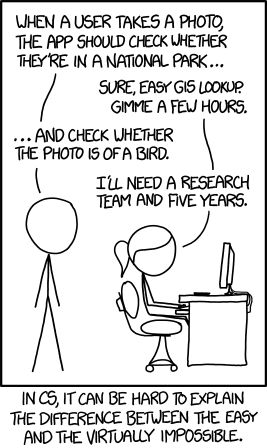
\includegraphics[width=0.4\textwidth]{./figures/introduction/xkcd_tasks.png}
  \caption{Moravec’s Paradox in popular literature~\cite{munroe2018tasks}.}
  \label{fig:introduction_xkcdtasks}
\end{figure}

To conclude, on one hand, new battery and processor designs established new robots and leveraged the solutions to problems, which held only theoretical value twenty years ago: for example the analysis of huge data blocks via machine learning (called ``big data'' analysis) or abstract learning via \glspl{ac:dnn}.
On the other hand, many problems are only solved via ``number crunching'': using the newly obtained computational power on huge data sets (an outstanding example is Google's image classification algorithm~\cite{krizhevsky2012imagenet}), while real \glspl{ac:ai} remain an open field of research.





\section{Motivation}
\label{ssec:introduction_motivation}

Many of the problems in robotics are simple for humans to solve, but remain incredibly demanding for machines.
The fields in robotics, which are touched by this simple example, range from image segmentation, tracking, classification, planning, and robot hardware design.
This paradox even has its own name ---  Moravec’s Paradox~\cite[p. 190]{pinker2003language}, also see \figref{fig:introduction_xkcdtasks}:

\begin{quote}
  ``The main lesson of thirty-five years of \gls{ac:ai} research is that the hard problems are easy and the easy problems are hard. The mental abilities of a four-year-old that we take for granted – recognizing a face, lifting a pencil, walking across a room, answering a question – in fact solve some of the hardest engineering problems ever conceived.''
\end{quote}

\begin{figure}
  \centering
  % Define block styles
\tikzstyle{block} = [draw, rectangle, fill=white, minimum height=3cm, minimum width=3.0cm, text width=2.9cm, text centered, rounded corners=true]
\tikzstyle{blockScene} = [draw, rectangle, fill=white, minimum height=3cm, minimum width=6.0cm, text width=5.9cm, text centered, rounded corners=true]
\tikzstyle{blockFit} = [draw, inner sep=0.2cm, dashed, rectangle, minimum width=3.0cm, text centered, rounded corners=true]
\tikzstyle{blockText} = [text centered, minimum height=1cm]
\tikzstyle{arrow} = [draw, -latex]

\definecolor{red1}{RGB}{160,0,0}
\definecolor{green1}{RGB}{0,160,0}
\definecolor{blue1}{RGB}{0,0,160}

% Define images
\pgfdeclareimage[height=2.5cm]{scene}{./figures/introduction/actionperceptionloop/scene.jpg}
	      
\begin{tikzpicture}[node distance = 8cm, auto]
  % Scene
  \node[blockScene] (scene_h) {\pgfuseimage{scene}};

	% Human
  \node [block, right of=scene_h, node distance=6cm] (eye_h) {\textbf{Human:}\\Vision, smell, taste, touch, \ldots};
  \node [block, below of=eye_h, node distance=5cm] (brain_h) {\textbf{Human:}\\Brain};
  \node [block, left of=brain_h, node distance=7.6cm]  (arm_h) {\textbf{Human:}\\Arms, legs, \ldots};

  % Robot
  \node [block, right of=eye_h, node distance=3.2cm] (eye_r) {\textbf{Robot:}\\Camera, gyroscope, accelerometer, \ldots};
  \node [block, right of=brain_h, node distance=3.2cm] (brain_r) {\textbf{Robot:}\\Computer Vision, planning, \ldots};
  \node [block, right of=arm_h, node distance=3.2cm] (arm_r) {\textbf{Robot:}\\Motors, wheels};

  % Text
  \node [blockText, above of=scene_h, color=red1, yshift=-6.06cm] (scene_t) {Scene};
  \node [blockText, above right of=eye_h, color=blue1, xshift=-4.0cm, yshift=-3.7cm] (eye_t) {Sensors};
  \node [blockText, above right of=brain_h, color=blue1, xshift=-4.0cm, yshift=-3.7cm] (brain_t) {Cognition};
  \node [blockText, above right of=arm_h, color=red1, xshift=-4.0cm, yshift=-3.7cm] (arm_t) {Actuators};

  % Fit
  \node[fit=(scene_h)(scene_t), blockFit] (scene) {};
  \node[fit=(eye_h)(eye_r)(eye_t), blockFit] (eye) {};
  \node[fit=(brain_h)(brain_r)(brain_t), blockFit] (brain) {};
  \node[fit=(arm_h)(arm_r)(arm_t), blockFit] (arm) {};

  % Arrows
	\path [arrow] (scene.east) to (eye.west);
	\path [arrow] (eye.south) to (brain.north);
	\path [arrow] (brain.west) to (arm.east);
	\path [arrow] (arm.north) to (scene.south);

  % Action-Perception side
  \node [blockText, below of=arm_t, color=red1, node distance=5cm] (action_t) {{\Huge Action side}};
  \node [blockText, below of=brain_t, color=blue1, node distance=5cm] (action_t) {{\Huge Perception side}};
\end{tikzpicture}

  \caption{Schematic diagram of the Action-Perception loop: A scene is re\-cor\-ded by sensors, second, the agent's cognition analyzes the input and forms a plan, which it executes via its actuators. These in turn act on the scene, where changes are again perceived by the sensors. The left side is therefore called ``action side'', and the right side is named ``perception side''.}
  \label{fig:introduction_actionperceptionloop}
\end{figure}

This problem statement can be formalized using a concept called Action-Per\-cep\-tion loop, which is shown in \figref{fig:introduction_actionperceptionloop}.
Each block from the loop contains its own problems in robotics: Starting from sensor noise and outlier detection, segmenting sensor input into meaningful symbols, preparing a feasible plan, and eventually executing said plan.
In this work, two systems are analyzed based on the Action-Perception loop.
The first system is based on a group of robots and will focus on the perception side.
An algorithm for noise and outlier reduction and an algorithm for estimating a robot's pose based on visual clues are introduced.

The second system focuses on the action side of the loop: An agent must be able to parse observations, therefore to create meaningful entities.
The state of each entity must be tracked over time.
Those in turn can be used as symbols in planning.
The plan must be transferred to the actuators, which execute the action.
One simple example would be: ``Picking up the apple''.
First, the sensor input, for example a RGB camera has to cluster the pixels into object candidates.
These candidates are classified with the results that one cluster is indeed an apple.
The plan consists of grasping the apple and lifting it, which can be performed using the robot hand.
It is easy to see that between the sensor input and the pixel cluster that forms the apple, exists a major difference in representation.
While on the one side there are raw pixel values, on the other side there is the symbol apple.
This difference is called signal-to-symbol gap.
High level symbolic representation is needed for planning~\cite{mcdermott1998}, but in robotics symbols always rely on raw sensor information.
When the robot executes an action, the gap has to be bridged the second time: Symbols have to be translated to motor currents.
The second system introduces a bottom-up method to bridge the signal-to-symbol gap and which allows for complex action planning.

This work is organized as follows: the next chapter after this introduction explains the first system, the following chapter analyzes the second system.
Both are followed by a detailed conclusion and outlook.



\chapter{From low level towards high level perception in robots}
\label{cha:perception}
\section{Introduction}
\label{perception_introduction}

In this chapter a robot is built, which manages to navigate based on its internal sensors only.
This means, it does not use \gls{ac:gps} or externally tracking to compute its own pose.
Furthermore, the here presented approach is entirely data-driven.
Thus, the robot can safely navigate in previously unknown, unstructured indoor or underground environments.


This section divides into two parts.
In the first part, there is a detailed description of a novel denoising filter called \gls{ac:epf}.
In environments with low ambient light conditions, any RGB camera introduces noisy pixels.
The filter removes this noise and replaces it with an averaged value of the local neighborhood.
It is shown that \gls{ac:epf} outperforms standard local denoising methods in quality while still running in real-time.
Global methods, however, show a slightly better performance, but their time performance range at about \unit[0.4]{Hz} and thus are far from real-time (and therefore not feasible in a robotic environment).
As the filter generalizes on any dimension, it can be also used on 1d sensor data, \eg readings from a gyroscope or accelerometer.


This is shown in the second part of this chapter.
Here, two ground based and one flying robot are introduced, which make use of the data filtering.
This enables the robots to use computer vision algorithms to localize themselves and share knowledge about the local environment.
A detailed analysis and comparison to start-of-the art is computed on two simulations: the here developed algorithms perform about twice as good as current state-of-the-art.
Furthermore, real-world office flights are shown.





\subsection{The state-of-the-art of denoising filters}

Real-time computer vision in fast moving robots still remains a challenging task, especially when forced to use limited computing power, as it is usually the case when implemented on embedded systems. 
Different light conditions are just one aspect of this vast field of problems.
Cameras (analog as well as digital cameras) introduce noise in poor light conditions, meaning in environments with low signal-to-noise ratio.
Removing this noise usually leads to better performance of object recognition tasks in 2d and 3d images, more stable computation of features, and improve tracking results.
In~\textcite{reichabramovpapon2013} it was shown  that removal of texture from 2d images significantly improves image segmentation results.
Parts of the results shown here are also published in~\textcite{reichwoergoetterdellen2018}.

An additional application is the automatic post-production of images, which are, generally speaking, more appealing to humans; there is a big community of photographers and we deem removing noise for pure aesthetic value as also important.
One application of the here presented filter is shown in \figref{fig:sensor_introduction_lena}.

Still, the filter generalizes well on arbitrary dimensions.
In a second part it is shown how to apply the same mechanisms to an arbitrary number of dimensions, enabling the filter to run on any physical measurement, for example on 1d sensor data obtained from an accelerometer, gyroscope, or \gls{ac:gps} tracker.

\begin{figure}
    \centering
    \begin{subfigure}[]{0.475\textwidth}
        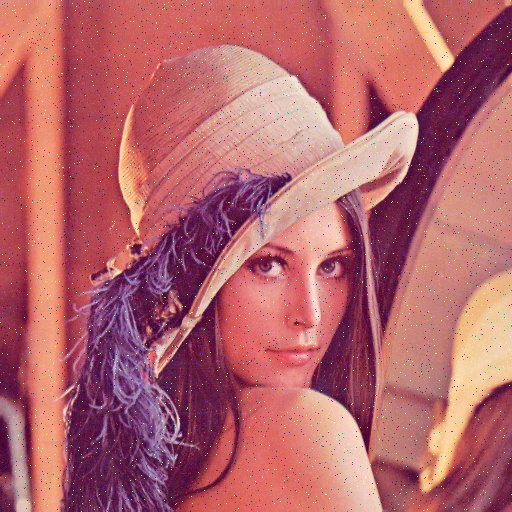
\includegraphics[width=\textwidth]{./figures/sensor/introduction_lena_noisy.jpg}
        \caption{Noisy test image.}
        \label{fig:sensor_introduction_lena_noisy}
    \end{subfigure}\hfill%
    \begin{subfigure}[]{0.475\textwidth}
        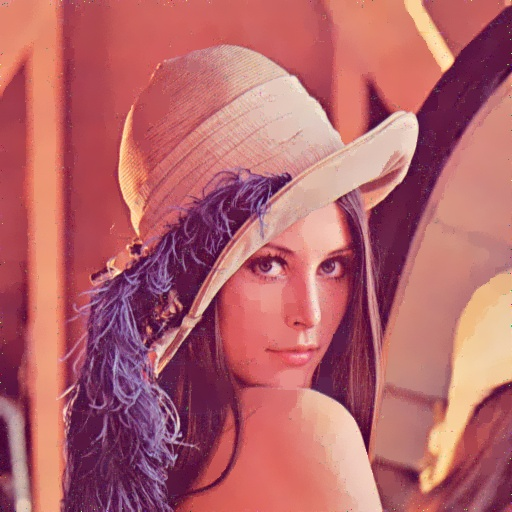
\includegraphics[width=\textwidth]{./figures/sensor/introduction_lena_edgefilter.jpg}
        \caption{Denoised test image.}
        \label{fig:sensor_introduction_lena_denoised}
	\end{subfigure}
  \caption{Even today, denoising remains a challenging task. The here proposed real-time denoising filter is called \gls{ac:epf}.}
  \label{fig:sensor_introduction_lena}
\end{figure}

Removing noise is a two-step process: First a noisy pixel needs to be identified as such, second it needs to be smoothed out. 
Both steps offer a wide range of problems.
In the first step a noisy pixel needs to be defined in a mathematical sense.
This means that a similarity criterion must be found.
However, similarities can exist on different scales, \ie between adjacent pixels or groups of pixels, as it is the case for texture.
In the second step a target value needs to be computed, which replaces the noisy pixel.
This target value should, again, only depend on the local neighborhood.

Removing noise has a long history in science. 
Most notable is the Gaussian Filter. 
It works by convoluting an image with a Gaussian function and thus works as a simple low-pass filter, attenuating high frequency signals~\cite[p. 257f]{gonzalezwoods2002}. 
As edges are also a high-frequency signal, they will be blurred out, too.

Noise in images is usually distinguished using a threshold. 
These thresholds can be either learned using a training set of images, as in support vector machines~\cite{yang2010svm} and \glspl{ac:ann}~\cite{muneyasu1995realization,pandey2016anatomization}, or the threshold may be computed from the surrounding pixel values, as in~\cite{du2011dynamic}. 
\cite{lev1977iterative} identified similar pixels by detecting edges and iteratively replacing the intensity of the pixel by the mean of all pixels in a small environment.

Another approach is presented in~\cite{tomasi1998bilateral}: The so called bilateral filter blurs neighboring pixels depending on their combined color and spatial distance. 
Hence, texture and noise, which has small deviation from the mean can be blurred without affecting boundaries. 
This leads to a trade-off: large blurring factors are needed to smooth out high level of noise, having the consequence that edges are not preserved anymore.

Another wide class of algorithms denoise by averaging. 
This averaging may happen locally as in the Gaussian smoothing model~\cite{lindenbaum1994gabor}, the anisotropic smoothing model~\cite{perona1990scale,alvarez1992image}, based on neighborhood filtering as in the already mentioned bilateral filter~\cite{tomasi1998bilateral}, using local variations as in~\cite{rudin1992nonlinear}, or based on the wavelet thresholding method~\cite{donoho1995noising}.

All these powerful methods have one common drawback: they all smooth small scaled noise and preserve color edges, however are not able to distinguish between a color edge and large scaled noise, \eg outliers. 
Outliers are a common problem in any sensor based application, as in accelerometers or gyroscopes, but also in 2d-RGB cameras, where high ISO settings often pose a big problem. 
More recent methods, which achieve this goal~\cite{dabov2007image,zoran2011learning,mairal2009non}, do not perform in real-time.
The approach presented here has the following features:

\begin{enumerate}
  \item smooths out small scaled noise,
  \item smooths out outliers,
  \item still preserves color edges, and
  \item performs in real-time.
\end{enumerate}





\subsection{The state-of-the-art of Visual Odometry}

The question how an agent using such a filter system behaves in a real-world scenario arises.
A real world agent allows to study behavioral patterns in more details, benchmark, and enhance quality of the algorithms.
The robot's platform should satisfy the following constraints:

\begin{itemize}
  \item the central computing board should be the same for all robots and powerful enough to perform computer vision tasks,
  \item the same code base should be used for all robots; hardware specific specialization should be off-loaded into separate code classes,
  \item sensors should be connectable via modern bus systems such as \wire\ and \ic,
  \item the framework should generalize well and should be easily extensible, and
  \item all robots should be able to communicate with each other via a central \gls{ac:wlan} node or peer-to-peer via Bluetooth.
\end{itemize}

It was decided to use a Raspberry Pi mini computer as computing platform.
Currently, it offers a quad-core \gls{ac:cpu} with \unit[1.4]{GHz}, a memory of \unit[1]{GB} and an onboard Bluetooth and \gls{ac:wlan} chip.
Additionally, an \gls{ac:imu} is attached to all robots, measuring lateral and rotational acceleration.
The robots are shown in \figref{fig:robot_introduction_photo}.
In total, there were two wheeled robots (\figref{fig:robot_introduction_photo_wheelpi}) and one flying robot, \figref{fig:robot_introduction_photo_flypi}, using a quadrotor design, built.

\begin{figure}
  \centering
  \begin{subfigure}[]{0.475\textwidth}
    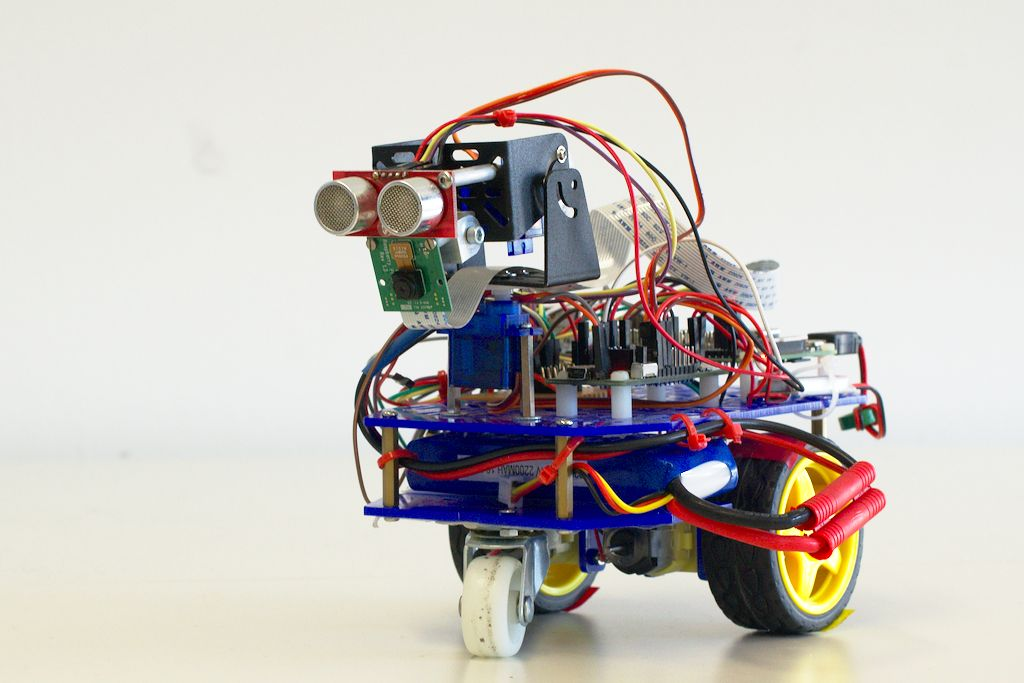
\includegraphics[width=1.0\textwidth]{./figures/robot/photos/wheelpi.jpg}
    \caption{WheelPi robot.}
    \label{fig:robot_introduction_photo_wheelpi}
  \end{subfigure}
  \hfill
  \begin{subfigure}[]{0.475\textwidth}
    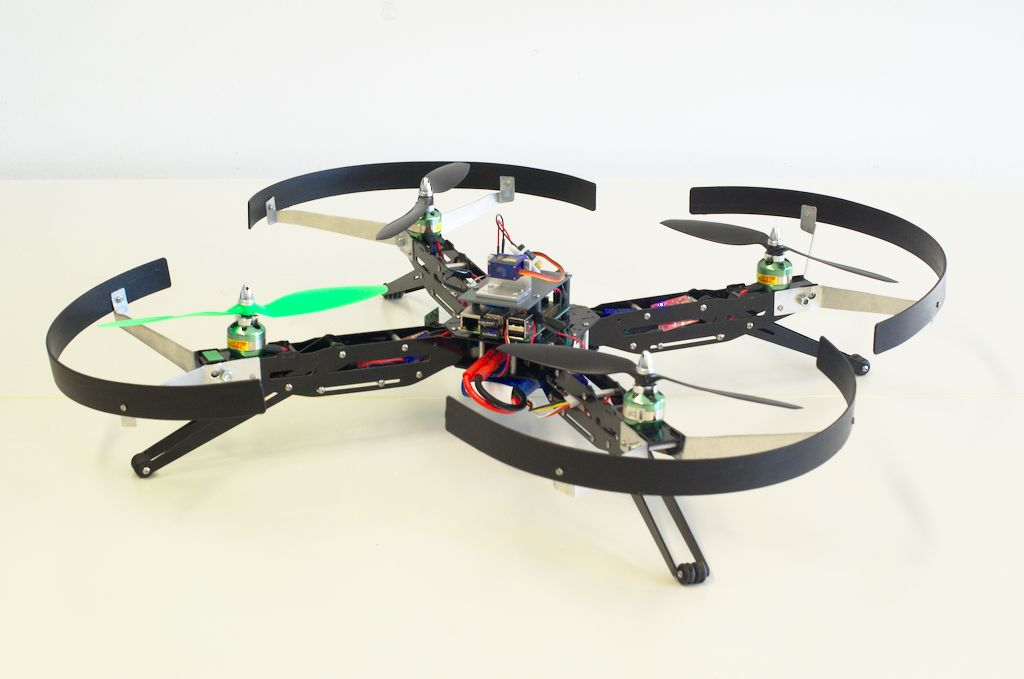
\includegraphics[width=1.0\textwidth]{./figures/robot/photos/quadcopter.jpg}
    \caption{FlyPi robot.}
    \label{fig:robot_introduction_photo_flypi}
  \end{subfigure}
  \caption{The pictures show the robots developed in this work. On the left, there is the WheelPi robot: a three-wheeled ground-based robot. In \figref{fig:robot_introduction_photo_flypi} the FlyPi robot is shown. It is a flying robot utilizing a quadrotor design. Both robots are part of the MovingPi library.}
  \label{fig:robot_introduction_photo}
\end{figure}

Given the constraints from above, the objective of this project is:

\begin{enumerate}
  \item Develop a framework, which can be easily deployed on different hardware designs,
  \item Utilize the framework on multiple agents,
  \item Each agent localizes itself in a previously unknown environment, and
  \item Information about the environment, \ie maps are shared across all agents.
\end{enumerate}

Parts of the here presented work is published in~\textcite{reichseerberscheid2018} and numerous students have contributed to this elaborate project.
They are listed above at the beginning of this thesis.

Humans may easily navigate inside a room.
We have stereo vision, allowing for 3d vision\footnote{At least most of us.}.
We can segment our visual field into subsets, where each subset represents a meaningful entity, \eg. an object.
Because we are able to perform all this intuitively, this is a deceptively tricky business.
One of the pioneers of \gls{ac:ai}, Marvin Minsky, invited to a summer school in 1966 called ``The Summer Vision Project''.
A Memo written by one of his research associates, Seymour Papert, outlines the project goals~\cite[p. 2f]{papert1966summer}:

\begin{enumerate}
  \item ``The primary goal\ldots\ is to\ldots\ divide a\ldots\ picture into regions such as
    \begin{itemize}
      \item likely objects
      \item likely background areas
      \item chaos.''
    \end{itemize}
  \item ``considerable analysis of shape and surface properties'' and ``region description''.
  \item ``The final goal is object identification which will actually name objects by matching them with a vocabulary of known objects.''
\end{enumerate}

Nearly half a century later, \glspl{ac:dnn} have shown promising results towards these goals~\cite{krizhevsky2012imagenet, deng2009imagenet, kim2014convolutional}.
Despite these extensive efforts to solve the ``construction of a significant part of a visual system''~\cite[p. 1]{papert1966summer}, a long road to complete ``computer vision'' remains.
In fact, this is just another form of Moravec's Paradox shown in \secref{ssec:introduction_motivation}; tasks, which are easy for human being are computational expensive for machines.

In this work, the focus lies on fully autonomous robots.
All computations must be performed on embedded hardware, \ie utilizing only limited computational power, and must run online in real-time.
Especially the flying robot, \figref{fig:robot_introduction_photo_flypi}, also named \gls{ac:aav}, must at all times provide safe error propagation and fallback settings.
On embedded hardware, without the support of large multi-core \glspl{ac:cpu} or \glspl{ac:gpu}, robots usually perform with a low frame rate.
One of the most challenging applications is visually guided on-board-com\-pu\-ted indoor flight.
There are no \gls{ac:gps} signals available and the autonomous vehicle has to navigate quickly in confined spaces.
To enable collision detection, onboard sensors have to be utilized.
Truly autonomous robots --- without mandatory connection to a stationary computing system --- and without the need of external sensors for navigation, may be used for example in indoor search-and-rescue missions, disaster relief in dangerous environments (as for example it was the case in Fukushima, Japan, 2011~\cite{chino2011preliminary}), reconnaissance, or underground mining operations.

In recent years, energy efficient, yet powerful hardware and batteries have become available.
Moreover, the physical dimensions of the hardware have been reduced a lot.
This allows on one hand for smaller robots and on the other hand for complex online motor control tasks and sensor evaluation --- as it is required in quadrocopters.
However, active sensor approaches pose the problem of high power consumption and heavy weight.
On today's robots, these problems are solved by using an RGB camera.
RGB cameras are passive sensors with low power consumption.

Previous work on autonomous flight can be categorized into two research areas.
First, many works focus on agile and accurate motion control. Most prominent is the quadrocopter swarm of ETH Zürich, which is able to perform synchronized dancing motions~\cite{schSPRI14}, build simple architectural structures~\cite{augugliaro2014flight}, or even knot strings and build a bridge~\cite{augugliaro2015knot}. 
But these complex tasks heavily rely on external tracking of the robots and are thus restricted to lab use~\cite{brescianini2018trajectory}. 
In another approach, artificial markers in the environment simplify pose estimation~\cite{eberli2011vision}. 
For \gls{ac:gps}-enabled areas, complete commercial solutions exist, \eg~\cite{vasarhelyi2014outdoor,radiansyah2017quadcopter}.

Second, there are approaches, which only use online sensors for self localization.
Still, in many studies the computationally expensive tasks are performed on external hardware via Bluetooth or \gls{ac:wlan} links, \eg~\cite{engel14ras,zhang2016controllable}, which limit the independence of the devices.
In recent years, the miniaturization of computers and advancements in battery design, driven mostly by rapid cell phone development, have made it possible to build smaller autonomous robots and perform computations in real-time on the \gls{ac:aav} itself.
While online computations result in maximum autonomy, even today, real-time computations on 3d data remain a too complex task.
Instead of 3d sensors such as LIDAR, the Asus Xtion Pro, or the Microsoft Kinect sensor, most systems use a monocular camera and perform 3d reconstruction.

For example, the detection of a planar landing zone for a helicopter using a monocular camera was described in~\cite{5584396} in 2010, allowing for autonomous landing of a helicopter.
Following up on this work, seven years later similar results are shown for a moving platform~\cite{falanga2017vision}.
Here, the robot relies only on its internal sensors and lands autonomously on a platform, which holds a marker and moves in a straight line with up to $\unit[4.2]{m/s}$.
\cite{6630807} use a front facing camera to detect objects in the flight path and estimate size.
In recent studies more stable SLAM methods were introduced, \eg~\cite{7219438,engel2014lsd,engel2017direct}, which promise good results for front-facing cameras.
However, these methods are computationally too expensive for embedded hardware.
Also, all approaches with a camera pointing to a specific direction face the problem of a small observation window with significant feature shifts in consecutive camera frames.

Omnidirectional monocular cameras, which provide a 360$\degree$ view of the environment, have been successfully applied to these problems.
Already in 2006 in~\cite{demonceaux2006omnidirectional} full attitude measurements were reported.
\cite{rodriguez2012real} apply this procedure to an unstable flying robot; however, no quantitative results are shown.
In~\cite{lukierski2017room}, a fast moving robot estimates the depth of edges in a corridor using an omnidirectional camera.
In~\cite{forster2014svo} a visual odometry algorithm is introduced, which tracks features and computes frame based pose displacement.
The authors report a frame rate of $\unit[55 \pm 1]{Hz}$, but computations are only performed on certain key frames.

In this work, the focus lies on navigating a flying robot in unknown, GPS-denied, indoor scenarios.
All computations are performed online and in real-time --- there will be no external tracking.
We ask: what is needed to safely (and therefore reliably) detect features on a hardware platform that strongly jerks, jolts, and may even flip?
And --- if those can be found --- how to track them and use them for trajectory planning on limited hardware in real-time?
One goal is to improve navigation by introducing a novel lightweight omnidirectional camera setup for embedded computer systems.
Lastly, the aim is to extract features, track them over multiple frames, compute a 3d point cloud, and perform high level navigation tasks on this internal model of the \gls{ac:aav}'s environment.

In the following section, we shortly introduce our hardware setup, a quadrocopter holding an omnidirectional camera.
Afterwards, the utilized algorithms, called \gls{ac:epf} and \gls{ac:evo}, are introduced.
This is followed by the results section.
First, \gls{ac:epf} is benchmarked on a real-world image data set and, second, experiments on artificial data are shown.
This is followed by three different experiments concerning \gls{ac:evo}: The system is benchmarked using two simulated scenarios and compared to recent methods.
Next, the performance is measured using external cameras to track the robot's position.
Third, a real-world office flight shows the viability of the approach.
The experiments are followed by a detailed discussion and conclusion.

\section{Methods}
\label{sec:perception_methods}


This section divides into three parts, which are shown in \figref{fig:perception_methods_flowchart}.
The a) hardware setup, namely the robots and camera, is presented in~\secref{ssec:perception_methods_hardwaresetup}.
The next section, \secref{ssec:perception_methods_noiseandoutlierdetection} shows b) how to detect noise and outliers and how to remove them.
The filter is described in the discrete, as well as continuous domain.
In c),~\secref{ssec:perception_methods_visualodometryalgorithm}, the algorithms to compute a pose update based only on Visual Odometry on embedded hardware are shown. 

\begin{figure}[]
  \centering
  % Define block styles
\tikzstyle{block} = [draw, rectangle, fill=white, minimum height=3.5cm, minimum width=6.0cm, text width=4.5cm, text centered, rounded corners=true]
\tikzstyle{blockBox} = [draw, inner sep=0.2cm, dashed, rectangle, minimum width=3.5cm, text centered, rounded corners=true]
\tikzstyle{blockText} = [text centered, minimum height=1.5cm,text width=5.0cm]
\tikzstyle{arrow} = [draw, -latex]

\definecolor{red1}{RGB}{160,0,0}
\definecolor{green1}{RGB}{0,160,0}
\definecolor{blue1}{RGB}{0,0,160}

% Define images
\pgfdeclareimage[height=3.0cm]{scene}{./figures/sensor/methods_flowchart_scene.jpg}
\pgfdeclareimage[height=3.0cm]{robot}{./figures/sensor/methods_flowchart_robot.jpg}
	      
\begin{tikzpicture}[node distance = 8.0cm, auto]
  % Scene
  \node[block] (scene) {\pgfuseimage{scene}};

  % Hardware setup
  \node [block, right of=scene] (hardwaresetup) {\pgfuseimage{robot}};

	% Filter
  \node [block, below of=scene, node distance=6.5cm] (filter) {Removing noise and outliers};
  
  % VO
  \node [block, right of=filter] (vo) {Estimating pose, position, and environment};
  

  % Text
  \node [blockText, above of=scene, node distance=2.5cm] (scene_t) {\textbf{a) Scene}};
  \node [blockText, above of=hardwaresetup, node distance=2.5cm] (hardwaresetup_t) {\textbf{b) Hardware setup}\\\secref{ssec:perception_methods_hardwaresetup}};
  \node [blockText, above of=filter, node distance=2.5cm] (filter_t) {\textbf{c) Preprocessing}\\\secref{ssec:perception_methods_noiseandoutlierdetection}};
  \node [blockText, above of=vo, node distance=2.5cm] (vo_t) {\textbf{d) Visual Odometry}\\\secref{ssec:perception_methods_visualodometryalgorithm}};


  % Fit
  \node[fit=(scene)(scene_t), blockBox] (scene_f) {};
  \node[fit=(hardwaresetup)(hardwaresetup_t), blockBox] (hardwaresetup_f) {};
  \node[fit=(filter)(filter_t), blockBox] (filter_f) {};
  \node[fit=(vo)(vo_t), blockBox] (vo_f) {};


  % Arrows
	\path [arrow] (scene_f.east) to (hardwaresetup_f.west);
	\path [arrow] (hardwaresetup_f.south) -| ++(0,-0.55cm) -| (filter_f.north);
	\path [arrow] (filter_f.east) to (vo_f.west);
\end{tikzpicture}

  \caption{Flowchart of the methods in this chapter and how they relate. Details are explained in \secref{sec:perception_methods}.}
  \label{fig:perception_methods_flowchart}
\end{figure}





\subsection{Hardware setup}
\label{ssec:perception_methods_hardwaresetup}

The hardware setup is depicted in \figref{fig:robot_introduction_photo}: A quadrocopter and a wheeled robot, both controlled by a Raspberry Pi mini computer.
As the focus lies on denoising and \gls{ac:vo} in this part of the thesis, mostly the quadrotor platform will be analyzed --- it is fast moving and therefore more demanding.
In order to cope with high turn rates in indoor environments, a catadioptric omnidirectional system is used.
It is composed of an upwards pointing monocular camera and a hyperbolic mirror above as shown in \figref{fig:robot_method_algorithms_mirror_hyperbolaphoto}.
The camera operates with a resolution of $\unit[480 \times\ 480]{px}$ at a frequency of \unit[30]{Hz}.
Additionally to the computer vision system, an \gls{ac:imu} is placed on the robot.
All software components run as modular and parallel nodes using \gls{ac:ros}.





\subsection{Noise and outlier detection}
\label{ssec:perception_methods_noiseandoutlierdetection}

Let $\Phi(i, j)$ be the observed image. 
Then the noisy image is defined as
\begin{align}
  \Phi\left(i,j\right) = u\left(i,j\right) + n\left(i,j\right),
\end{align}
where $u\left(i,j\right)$ is the ``true'' value and $n\left(i,j\right)$ is noise at image position $\left(i,j\right)^T$. 
Here, noise is modeled as Gaussian white noise, meaning $n\left(i,j\right)$ is Gaussian distributed with zero mean and variance $\sigma^2$.
Additionally, salt-and-pepper noise is added: a fixed percentage of color channels will be set to either $0$ or its maximum value.
The filter $D_h$, with filter parameter $h$, is defined as follows
\begin{align}
  \Phi &= D_{h}(\Phi) + n
\end{align}
meaning, that for an optimal filter
\begin{align}
  u &= D_h(u+n)
\end{align}
should be true. 
The filter parameter $h$ should depend only on the variance of the noise $h = h(\sigma)$. 
Later, for evaluation the \gls{ac:rmse} and \gls{ac:psnr} between the original image $u$ and the filtered $D_h(u+n)$ is computed.


\begin{figure}[t]
  \centering
  % Define block styles
\tikzstyle{block} = [draw, rectangle, fill=white, minimum height=3cm, minimum width=3.9cm, text width=3.7cm, text centered, rounded corners=true]
\tikzstyle{blockBox} = [draw, inner sep=0.2cm, dashed, rectangle, minimum width=3.5cm, text centered, rounded corners=true]
\tikzstyle{blockText} = [text centered, minimum height=1.5cm,text width=3.9cm]
\tikzstyle{blockS} = [text centered, text width=1.1cm, minimum height=0.5cm, rounded corners=true, fill=white]
\tikzstyle{arrow} = [draw, -latex]

\definecolor{red1}{RGB}{160,0,0}
\definecolor{green1}{RGB}{0,160,0}
\definecolor{blue1}{RGB}{0,0,160}

% Define images
\pgfdeclareimage[height=2.8cm]{scene}{./figures/perception/methods/visualodometryalgorithm/flowchart_scene.jpg}
\pgfdeclareimage[height=2.8cm]{features}{./figures/perception/methods/visualodometryalgorithm/flowchart_features_frame.jpg}
\pgfdeclareimage[width=3.6cm]{transform}{./figures/perception/methods/visualodometryalgorithm/flowchart_transform.jpg}
\pgfdeclareimage[height=2.4cm]{triangulation}{./figures/perception/methods/visualodometryalgorithm/flowchart_triangulation.png}
\pgfdeclareimage[height=2.8cm]{pointcloud}{./figures/perception/methods/visualodometryalgorithm/flowchart_pointcloud_small.jpg}

\newsavebox\mybox
\begin{lrbox}{\mybox}
  \begin{tikzpicture}[node distance=1.5cm, auto]
    \node [blockS] (s1) {\small{VO\\6~DoF}};
    \node [blockS, right of=s1] (s2) {\small{IMU\\6~DoF}};
    %\node [blockS, below of=s1, node distance=1cm] (s4) {\pgfuseimage{picRottrans}};
    \node [blockS, below of=s1, xshift=0.75cm, node distance=1.25cm, text width=2.5cm] (s3) {\small{EKF}};

    \draw [arrow] (s1.south) to (s3.north);
    \draw [arrow] (s2.south) to (s3.north);
  \end{tikzpicture}
\end{lrbox}

	      
\begin{tikzpicture}[node distance = 5.0cm, auto]
  % Scene
  \node[block] (scene) {\pgfuseimage{scene}};

	% Features and Optical flow
  \node [block, right of=scene] (features) {\pgfuseimage{features}};

  % Transform
  \node [block, right of=features] (transform) {\pgfuseimage{transform}};
  

  % EKF
  \node [block, below of=scene, node distance=6.0cm] (ekf) {\usebox\mybox};
  
  % Depth
  \node [block, right of=ekf] (triangulation) {\pgfuseimage{triangulation}};
  
  % Point Cloud
  \node [block, right of=triangulation] (pointcloud) {\pgfuseimage{pointcloud}};
  
  
  % Text
  \node [blockText, above of=scene, node distance=2.2cm] (scene_t) {\textbf{a) Scene}};
  \node [blockText, above of=features, node distance=2.2cm] (features_t) {\textbf{b) Features and optical flow}};
  \node [blockText, above of=transform, node distance=2.2cm] (transform_t) {\textbf{c) Dewarp}};
  \node [blockText, above of=ekf, node distance=2.2cm] (ekf_t) {\textbf{d) Fuse}};
  \node [blockText, above of=triangulation, node distance=2.2cm] (triangulation_t) {\textbf{e) Compute depth}};
  \node [blockText, above of=pointcloud, node distance=2.2cm] (pointcloud_t) {\textbf{f) Generate point cloud}};


  % Fit
  \node[fit=(scene)(scene_t), blockBox] (scene_f) {};
  \node[fit=(features)(features_t), blockBox] (features_f) {};
  \node[fit=(transform)(transform_t), blockBox] (tranform_f) {};
  \node[fit=(ekf)(ekf_t), blockBox] (ekf_f) {};
  \node[fit=(triangulation)(triangulation_t), blockBox] (triangulation_f) {};
  \node[fit=(pointcloud)(pointcloud_t), blockBox] (pointcloud_f) {};


  % Arrows
	\path [arrow] (scene_f.east) to (features_f.west);
	\path [arrow] (features_f.east) to (tranform_f.west);
	\path [arrow] (tranform_f.south) -| ++(0,-0.55cm) -| (ekf_f.north);
	\path [arrow] (ekf_f.east) to (triangulation_f.west);
	\path [arrow] (triangulation_f.east) to (pointcloud_f.west);
\end{tikzpicture}

    \caption{Overview of the system structure. A detailed explanation of all steps is shown in \secref{ssec:perception_methods_noiseandoutlierdetection}.}
  \label{fig:perception_methods_noiseandoutlierremoval_flowchart}
\end{figure}

A flowchart of the proposed algorithm \gls{ac:epf} is shown in \figref{fig:perception_methods_noiseandoutlierremoval_flowchart}, a detailed explanation of all steps follows in the next sections.
First, the image $\Phi$ is divided into a) subwindows $\Psi$ sized $N = k \cdot l$, where each subwindow is shifted by one pixel relative to the last one, such that there are as many subwindows as there are pixels in the image. 
Each subwindow is then b) smoothed using a Gaussian kernel. 
Subwindow size $k \times l$ and Gaussian smoothing parameter are hyperparameters, which need to be manually tuned.
However, all three heavily depend on the amount of noise you would want to remove. 
For each subwindow centered around pixel position $(i, j)^T$ a c) distance matrix $\Delta_{i,j}$ and a mean distance $\delta_{i,j}^m$ is computed in the color domain. 
This offers a measurement for noise, as described below. 
A user selected d) threshold $\tau$, which defines a threshold between noise and a mere color edge, is applied to $\Delta_{i,j}$ and $\delta_{i,j}^m$. 
In case of noise, e) a weight $\omega_{i,j}$ is computed, which will move the color values of the pixel in the subwindow to the mean color of the subwindow.

\begin{figure}
    \centering
    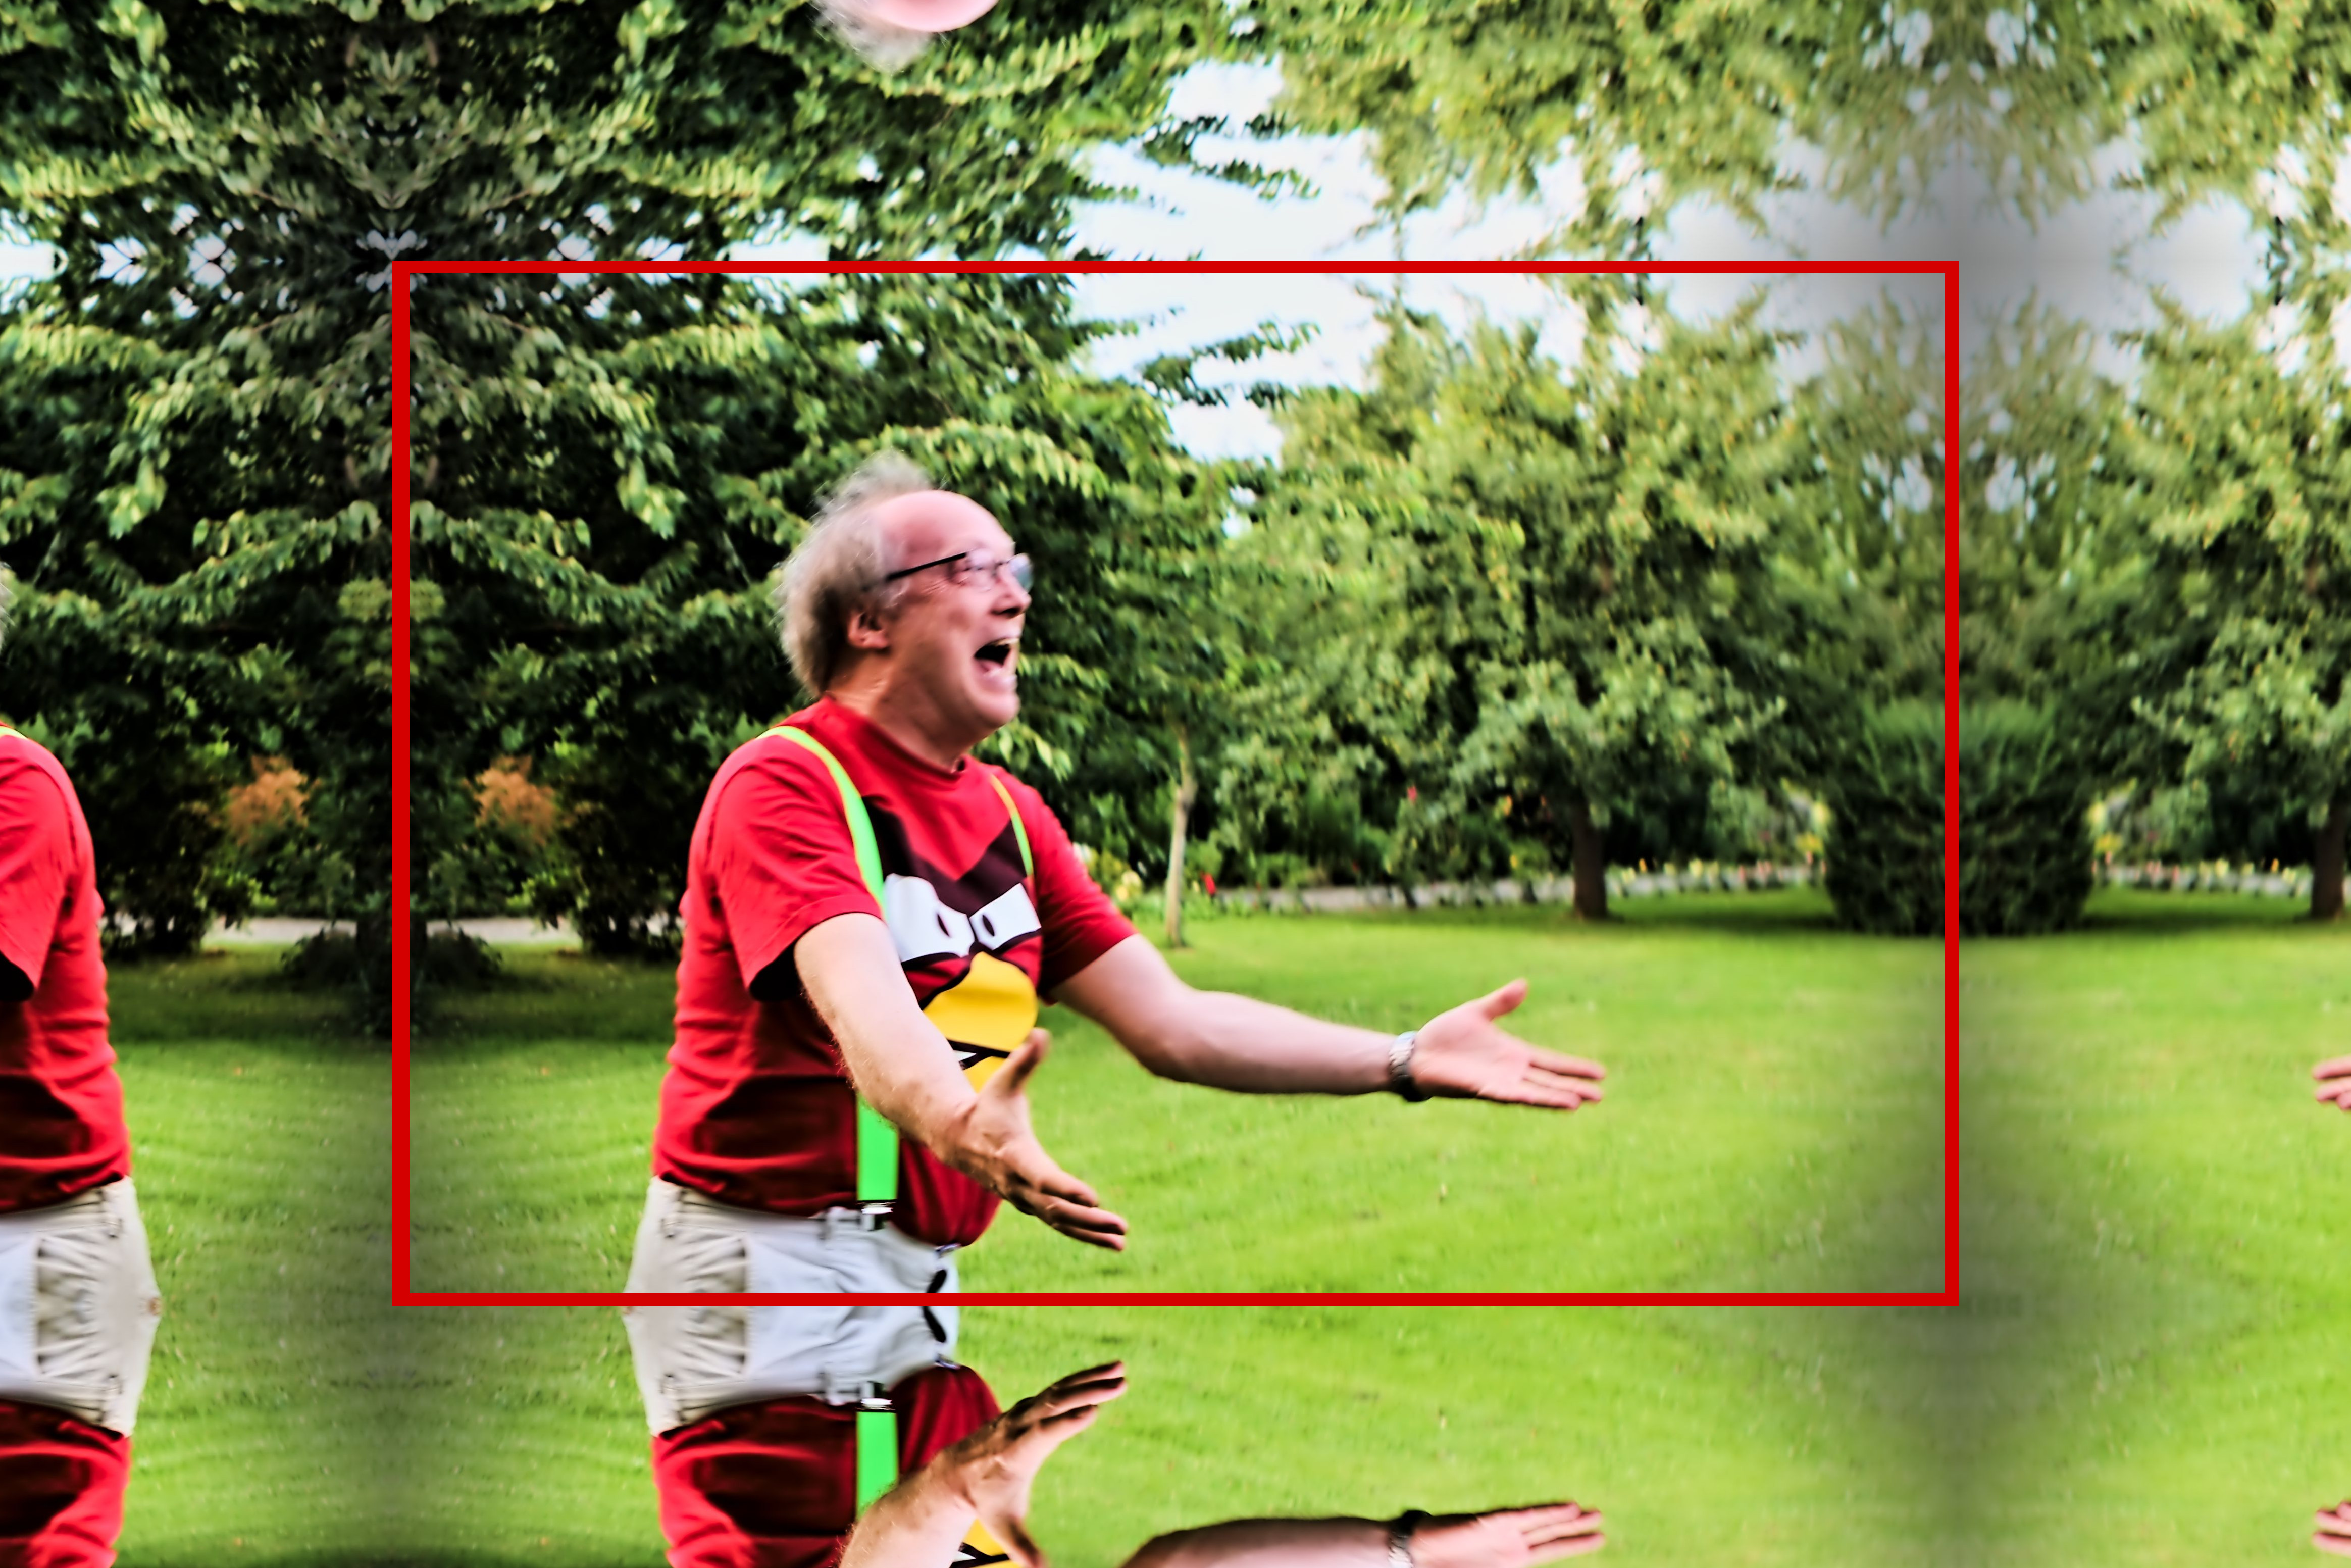
\includegraphics[width=0.75\textwidth]{./figures/sensor/method_boundaryconditions.jpg}
    \caption{Periodic mirrored boundary conditions are used for image subwindows. A red rectangle denotes borders of original image.}
    \label{fig:method_boundaryconditions}
\end{figure}





\subsubsection{Division into subwindows} 

Let one pixel at position $(i, j)^T$ contain the color information
\begin{eqnarray}
   \bm{\varphi}_{i,j} = ( \varphi_{i,j}^r,\ \varphi_{i,j}^g,\ \varphi_{i,j}^b )^T. 
\end{eqnarray}
A subwindow $\Psi^{\left(i,j\right)}$ is created around $(i, j)^T$, such that $(i, j)^T$ is centered. 
In case the subwindow contains an image boundary, periodic mirrored boundary conditions are used as visualized in \figref{fig:method_boundaryconditions}. 
The size of the subwindow is defined by $k \times l$ and a pixel's position inside the subwindow will be denoted by $(r, s)^T$.
This implies $0 \leq r < k$ and $0 \leq s < l$. 
Please note that other than rectangular shaped windows are possible.
In this work, additionally disc-shaped and Gaussian shaped subwindows were tried, however results differed only marginally.





\subsubsection{Smoothing} 

Each subwindow is smoothed via a Gaussian kernel~\cite[p. 257f]{gonzalezwoods2002}. 
This removes outliers, which would otherwise distort the computation of the mean as described in the next step.





\subsubsection{Computation of the distance matrix}

For each subwindow $\Psi^{\left(i,j\right)}$ the arithmetic mean is calculated as
\begin{eqnarray}
  \bm{\psi}_{m}^{\left(i,j\right)} = \frac{1}{N} \left( \sum_{r,s} \psi_{r,s}^r,\ \sum_{r,s} \psi_{r,s}^g,\ \sum_{r,s} \psi_{r,s}^b \right)^T
\end{eqnarray}
where $N = k \cdot l$ denotes the size of the subwindow. The pixelwise distances
\begin{eqnarray}
  \delta_{r,s}^{\left(i,j\right)} = | \bm{\psi}_{r,s} - \bm{\psi}_{m}^{\left(i,j\right)} |_2
\end{eqnarray}
are stored in a matrix $\Delta^{\left(i,j\right)}$. Furthermore, for each subwindow $\Psi^{\left(i,j\right)}$ the mean pixelwise distance 
\begin{eqnarray}
  \delta_m^{\left(i,j\right)} = \frac{1}{N} \sum_{r,s} \delta_{r,s}^{\left(i,j\right)}
\end{eqnarray}
is calculated.





\subsubsection{Thresholding}

Using a threshold it is now analyzed, whether a subwindow contains a color edge (and therefore no pixels should be smoothed), whether one pixel contains an outlier (and should be corrected), or neither, which means the pixel value should also not be replaced.
If $\delta_m^{\left(i,j\right)}$ is large, the subwindow contains big color variations.
This means the subwindow includes a color edge.
If $\delta_m^{\left(i,j\right)}$ is small, but one single pixel holds a big color variations (large $\delta_{r,s}^{\left(i,j\right)}$), there is an outlier, which needs to be replaced.
If both, $\delta_m^{\left(i,j\right)}$ and $\delta_{r,s}^{\left(i,j\right)}$ are small, the pixel holds a ``normal color'' value.
A threshold $\tau$ is introduced to identify noisy pixels and color edges, yielding
\begin{eqnarray}
  \psi_{r,s} =  \begin{cases}
    \textrm{color\ edge} & \textrm{,\ if\ } \delta_m^{\left(i,j\right)} > \tau, \\
    \textrm{noise} & \textrm{,\ if\ } \delta_m^{\left(i,j\right)} \leq \tau \textrm{\ and\ } \delta_{r,s} > \tau, \\
    \textrm{neither} & \textrm{,\ else}.
  \end{cases} \label{eqn:decision_noise_edge}
\end{eqnarray}





\subsubsection{Update of RGB values}

A new image $\Theta$, holding the pixel values $\bm{\theta}_{i,j}$ is computed based upon the squared distance of the user based threshold $\tau$ and the pixelwise distance $\delta_{r,s}$. 
$\bm{\theta}_{i,j}$ is updated as follows
\begin{eqnarray}
  \bm{\theta}_{i,j} &\longleftarrow& \bm{\theta}_{i,j} + \psi_{r,s} \cdot \left( \tau - \delta_{r,s}^{\left(i,j\right)} \right)^2 \cdot \bm{\psi}_{m}^{\left(i,j\right)}.
\end{eqnarray}
Please note, that due to the sliding subwindows each pixel is updated $N= k \cdot l$ times and therefore needs to be normalized. Thus, an additional weight $\Omega$ is introduced for each pixel $\omega_{i,j}$ as
\begin{eqnarray}
  \omega_{i,j} &\longleftarrow& \omega_{i,j} + \psi_{r,s} \cdot \left( \tau - \delta_{r,s}^{\left(i,j\right)} \right)^2.
  \label{eq:method_weightupdate}
\end{eqnarray}
The final image results from division of $\Theta$ by $\Omega$. 
In rare cases $\tau = \delta_{r,s}^{\left(i,j\right)}$ for large image patches may happen, which will result in $\omega_{i,j} = 0$ according to \eqnref{eq:method_weightupdate}.
To avoid division by zero it is suggested to initialize $\Omega$ with ones instead of zeros (since in general $\omega_{i,j} \gg 0$, this does not change the final outcome significantly).

\begin{figure}
  \centering
  \begin{tikzpicture}[gnuplot]
%% generated with GNUPLOT 5.2p2 (Gentoo revision r0) (Lua 5.1; terminal rev. 99, script rev. 102)
%% Fri 08 Jun 2018 01:36:24 PM CEST
\gpcolor{color=gp lt color border}
\gpsetlinetype{gp lt border}
\gpsetdashtype{gp dt solid}
\gpsetlinewidth{1.00}
\draw[gp path] (1.354,1.842)--(1.568,1.842);
\node[gp node right] at (1.354,1.842) {$10$};
\draw[gp path] (1.354,3.176)--(1.568,3.176);
\node[gp node right] at (1.354,3.176) {$20$};
\draw[gp path] (1.354,4.508)--(1.568,4.508);
\node[gp node right] at (1.354,4.508) {$30$};
\draw[gp path] (1.354,5.842)--(1.568,5.842);
\node[gp node right] at (1.354,5.842) {$40$};
\draw[gp path] (1.354,7.176)--(1.568,7.176);
\node[gp node right] at (1.354,7.176) {$50$};
\draw[gp path] (1.354,8.508)--(1.568,8.508);
\node[gp node right] at (1.354,8.508) {$60$};
\draw[gp path] (1.354,1.175)--(1.354,1.390);
\node[gp node center] at (1.354,0.808) {$0$};
\draw[gp path] (2.414,1.175)--(2.414,1.390);
\node[gp node center] at (2.414,0.808) {$10$};
\draw[gp path] (3.475,1.175)--(3.475,1.390);
\node[gp node center] at (3.475,0.808) {$20$};
\draw[gp path] (4.536,1.175)--(4.536,1.390);
\node[gp node center] at (4.536,0.808) {$30$};
\draw[gp path] (5.596,1.175)--(5.596,1.390);
\node[gp node center] at (5.596,0.808) {$40$};
\draw[gp path] (6.657,1.175)--(6.657,1.390);
\node[gp node center] at (6.657,0.808) {$50$};
\draw[gp path] (7.717,1.175)--(7.717,1.390);
\node[gp node center] at (7.717,0.808) {$60$};
\draw[gp path] (8.778,1.175)--(8.778,1.390);
\node[gp node center] at (8.778,0.808) {$70$};
\draw[gp path] (9.839,1.175)--(9.839,1.390);
\node[gp node center] at (9.839,0.808) {$80$};
\draw[gp path] (10.899,1.175)--(10.899,1.390);
\node[gp node center] at (10.899,0.808) {$90$};
\draw[gp path] (1.354,9.175)--(1.354,1.175)--(11.854,1.175)--(11.854,9.175)--cycle;
\draw[gp path](1.990,2.108)--(2.234,5.976);
\draw[gp path](2.839,2.108)--(5.596,5.976);
\draw[gp path](6.233,2.108)--(7.866,3.602);
\draw[gp path](7.081,8.109)--(7.866,6.308);
\draw[gp path](-0.373,2.255)--(1.354,1.175);
\draw[gp path](-0.373,7.415)--(1.354,9.175);
\node[gp node center,rotate=-270] at (0.329,5.175) {grayscale value};
\node[gp node center] at (6.603,0.256) {pixel number};
\gpcolor{rgb color={0.667,0.000,0.000}}
\gpsetlinewidth{2.00}
\gpsetpointsize{4.00}
\gppoint{gp mark 2}{(1.354,1.801)}
\gppoint{gp mark 2}{(1.460,1.824)}
\gppoint{gp mark 2}{(1.566,1.902)}
\gppoint{gp mark 2}{(1.672,1.848)}
\gppoint{gp mark 2}{(1.778,1.746)}
\gppoint{gp mark 2}{(1.884,1.735)}
\gppoint{gp mark 2}{(1.990,1.767)}
\gppoint{gp mark 2}{(2.096,1.809)}
\gppoint{gp mark 2}{(2.202,2.048)}
\gppoint{gp mark 2}{(2.308,1.711)}
\gppoint{gp mark 2}{(2.414,5.175)}
\gppoint{gp mark 2}{(2.520,1.831)}
\gppoint{gp mark 2}{(2.626,1.785)}
\gppoint{gp mark 2}{(2.733,2.041)}
\gppoint{gp mark 2}{(2.839,2.018)}
\gppoint{gp mark 2}{(2.945,1.898)}
\gppoint{gp mark 2}{(3.051,1.962)}
\gppoint{gp mark 2}{(3.157,1.840)}
\gppoint{gp mark 2}{(3.263,1.866)}
\gppoint{gp mark 2}{(3.369,1.467)}
\gppoint{gp mark 2}{(3.475,1.509)}
\gppoint{gp mark 2}{(3.581,1.894)}
\gppoint{gp mark 2}{(3.687,1.752)}
\gppoint{gp mark 2}{(3.793,1.986)}
\gppoint{gp mark 2}{(3.899,1.840)}
\gppoint{gp mark 2}{(4.005,1.897)}
\gppoint{gp mark 2}{(4.111,2.020)}
\gppoint{gp mark 2}{(4.217,1.570)}
\gppoint{gp mark 2}{(4.323,1.976)}
\gppoint{gp mark 2}{(4.430,2.082)}
\gppoint{gp mark 2}{(4.536,1.746)}
\gppoint{gp mark 2}{(4.642,2.172)}
\gppoint{gp mark 2}{(4.748,1.683)}
\gppoint{gp mark 2}{(4.854,1.783)}
\gppoint{gp mark 2}{(4.960,1.779)}
\gppoint{gp mark 2}{(5.066,1.704)}
\gppoint{gp mark 2}{(5.172,1.940)}
\gppoint{gp mark 2}{(5.278,2.145)}
\gppoint{gp mark 2}{(5.384,1.950)}
\gppoint{gp mark 2}{(5.490,1.967)}
\gppoint{gp mark 2}{(5.596,1.706)}
\gppoint{gp mark 2}{(5.702,2.169)}
\gppoint{gp mark 2}{(5.808,1.600)}
\gppoint{gp mark 2}{(5.914,1.823)}
\gppoint{gp mark 2}{(6.020,2.013)}
\gppoint{gp mark 2}{(6.126,1.758)}
\gppoint{gp mark 2}{(6.233,1.818)}
\gppoint{gp mark 2}{(6.339,1.825)}
\gppoint{gp mark 2}{(6.445,1.447)}
\gppoint{gp mark 2}{(6.551,1.800)}
\gppoint{gp mark 2}{(6.657,8.518)}
\gppoint{gp mark 2}{(6.763,8.551)}
\gppoint{gp mark 2}{(6.869,8.551)}
\gppoint{gp mark 2}{(6.975,8.559)}
\gppoint{gp mark 2}{(7.081,8.753)}
\gppoint{gp mark 2}{(7.187,8.274)}
\gppoint{gp mark 2}{(7.293,8.567)}
\gppoint{gp mark 2}{(7.399,8.396)}
\gppoint{gp mark 2}{(7.505,8.571)}
\gppoint{gp mark 2}{(7.611,8.540)}
\gppoint{gp mark 2}{(7.717,8.798)}
\gppoint{gp mark 2}{(7.823,8.441)}
\gppoint{gp mark 2}{(7.930,8.810)}
\gppoint{gp mark 2}{(8.036,8.531)}
\gppoint{gp mark 2}{(8.142,8.536)}
\gppoint{gp mark 2}{(8.248,8.519)}
\gppoint{gp mark 2}{(8.354,8.468)}
\gppoint{gp mark 2}{(8.460,8.511)}
\gppoint{gp mark 2}{(8.566,8.549)}
\gppoint{gp mark 2}{(8.672,8.525)}
\gppoint{gp mark 2}{(8.778,8.396)}
\gppoint{gp mark 2}{(8.884,8.526)}
\gppoint{gp mark 2}{(8.990,8.655)}
\gppoint{gp mark 2}{(9.096,8.433)}
\gppoint{gp mark 2}{(9.202,8.509)}
\gppoint{gp mark 2}{(9.308,8.667)}
\gppoint{gp mark 2}{(9.414,8.500)}
\gppoint{gp mark 2}{(9.520,8.266)}
\gppoint{gp mark 2}{(9.626,8.292)}
\gppoint{gp mark 2}{(9.733,8.642)}
\gppoint{gp mark 2}{(9.839,8.326)}
\gppoint{gp mark 2}{(9.945,8.651)}
\gppoint{gp mark 2}{(10.051,8.451)}
\gppoint{gp mark 2}{(10.157,8.290)}
\gppoint{gp mark 2}{(10.263,8.469)}
\gppoint{gp mark 2}{(10.369,8.643)}
\gppoint{gp mark 2}{(10.475,8.528)}
\gppoint{gp mark 2}{(10.581,8.559)}
\gppoint{gp mark 2}{(10.687,8.394)}
\gppoint{gp mark 2}{(10.793,8.449)}
\gppoint{gp mark 2}{(10.899,8.429)}
\gppoint{gp mark 2}{(11.005,8.357)}
\gppoint{gp mark 2}{(11.111,8.521)}
\gppoint{gp mark 2}{(11.217,8.471)}
\gppoint{gp mark 2}{(11.323,8.345)}
\gppoint{gp mark 2}{(11.430,8.345)}
\gppoint{gp mark 2}{(11.536,8.440)}
\gppoint{gp mark 2}{(11.642,8.401)}
\gppoint{gp mark 2}{(11.748,8.348)}
\gppoint{gp mark 2}{(11.854,8.401)}
\gpcolor{rgb color={0.000,0.000,0.667}}
\gppoint{gp mark 1}{(1.354,1.822)}
\gppoint{gp mark 1}{(1.460,1.820)}
\gppoint{gp mark 1}{(1.566,1.822)}
\gppoint{gp mark 1}{(1.672,1.823)}
\gppoint{gp mark 1}{(1.778,1.822)}
\gppoint{gp mark 1}{(1.884,1.820)}
\gppoint{gp mark 1}{(1.990,1.818)}
\gppoint{gp mark 1}{(2.096,1.819)}
\gppoint{gp mark 1}{(2.202,1.826)}
\gppoint{gp mark 1}{(2.308,1.820)}
\gppoint{gp mark 1}{(2.414,2.239)}
\gppoint{gp mark 1}{(2.520,1.856)}
\gppoint{gp mark 1}{(2.626,1.838)}
\gppoint{gp mark 1}{(2.733,1.837)}
\gppoint{gp mark 1}{(2.839,1.828)}
\gppoint{gp mark 1}{(2.945,1.822)}
\gppoint{gp mark 1}{(3.051,1.817)}
\gppoint{gp mark 1}{(3.157,1.812)}
\gppoint{gp mark 1}{(3.263,1.811)}
\gppoint{gp mark 1}{(3.369,1.806)}
\gppoint{gp mark 1}{(3.475,1.803)}
\gppoint{gp mark 1}{(3.581,1.811)}
\gppoint{gp mark 1}{(3.687,1.814)}
\gppoint{gp mark 1}{(3.793,1.831)}
\gppoint{gp mark 1}{(3.899,1.838)}
\gppoint{gp mark 1}{(4.005,1.850)}
\gppoint{gp mark 1}{(4.111,1.860)}
\gppoint{gp mark 1}{(4.217,1.860)}
\gppoint{gp mark 1}{(4.323,1.873)}
\gppoint{gp mark 1}{(4.430,1.880)}
\gppoint{gp mark 1}{(4.536,1.878)}
\gppoint{gp mark 1}{(4.642,1.882)}
\gppoint{gp mark 1}{(4.748,1.874)}
\gppoint{gp mark 1}{(4.854,1.875)}
\gppoint{gp mark 1}{(4.960,1.875)}
\gppoint{gp mark 1}{(5.066,1.878)}
\gppoint{gp mark 1}{(5.172,1.888)}
\gppoint{gp mark 1}{(5.278,1.892)}
\gppoint{gp mark 1}{(5.384,1.890)}
\gppoint{gp mark 1}{(5.490,1.887)}
\gppoint{gp mark 1}{(5.596,1.873)}
\gppoint{gp mark 1}{(5.702,1.871)}
\gppoint{gp mark 1}{(5.808,1.863)}
\gppoint{gp mark 1}{(5.914,1.861)}
\gppoint{gp mark 1}{(6.020,1.860)}
\gppoint{gp mark 1}{(6.126,1.843)}
\gppoint{gp mark 1}{(6.233,1.830)}
\gppoint{gp mark 1}{(6.339,1.818)}
\gppoint{gp mark 1}{(6.445,1.800)}
\gppoint{gp mark 1}{(6.551,1.805)}
\gppoint{gp mark 1}{(6.657,8.526)}
\gppoint{gp mark 1}{(6.763,8.527)}
\gppoint{gp mark 1}{(6.869,8.538)}
\gppoint{gp mark 1}{(6.975,8.539)}
\gppoint{gp mark 1}{(7.081,8.546)}
\gppoint{gp mark 1}{(7.187,8.546)}
\gppoint{gp mark 1}{(7.293,8.551)}
\gppoint{gp mark 1}{(7.399,8.552)}
\gppoint{gp mark 1}{(7.505,8.556)}
\gppoint{gp mark 1}{(7.611,8.561)}
\gppoint{gp mark 1}{(7.717,8.567)}
\gppoint{gp mark 1}{(7.823,8.564)}
\gppoint{gp mark 1}{(7.930,8.564)}
\gppoint{gp mark 1}{(8.036,8.556)}
\gppoint{gp mark 1}{(8.142,8.554)}
\gppoint{gp mark 1}{(8.248,8.545)}
\gppoint{gp mark 1}{(8.354,8.538)}
\gppoint{gp mark 1}{(8.460,8.533)}
\gppoint{gp mark 1}{(8.566,8.528)}
\gppoint{gp mark 1}{(8.672,8.520)}
\gppoint{gp mark 1}{(8.778,8.512)}
\gppoint{gp mark 1}{(8.884,8.508)}
\gppoint{gp mark 1}{(8.990,8.505)}
\gppoint{gp mark 1}{(9.096,8.500)}
\gppoint{gp mark 1}{(9.202,8.496)}
\gppoint{gp mark 1}{(9.308,8.490)}
\gppoint{gp mark 1}{(9.414,8.480)}
\gppoint{gp mark 1}{(9.520,8.470)}
\gppoint{gp mark 1}{(9.626,8.468)}
\gppoint{gp mark 1}{(9.733,8.472)}
\gppoint{gp mark 1}{(9.839,8.469)}
\gppoint{gp mark 1}{(9.945,8.472)}
\gppoint{gp mark 1}{(10.051,8.470)}
\gppoint{gp mark 1}{(10.157,8.468)}
\gppoint{gp mark 1}{(10.263,8.471)}
\gppoint{gp mark 1}{(10.369,8.477)}
\gppoint{gp mark 1}{(10.475,8.477)}
\gppoint{gp mark 1}{(10.581,8.472)}
\gppoint{gp mark 1}{(10.687,8.462)}
\gppoint{gp mark 1}{(10.793,8.456)}
\gppoint{gp mark 1}{(10.899,8.445)}
\gppoint{gp mark 1}{(11.005,8.438)}
\gppoint{gp mark 1}{(11.111,8.433)}
\gppoint{gp mark 1}{(11.217,8.422)}
\gppoint{gp mark 1}{(11.323,8.410)}
\gppoint{gp mark 1}{(11.430,8.402)}
\gppoint{gp mark 1}{(11.536,8.398)}
\gppoint{gp mark 1}{(11.642,8.395)}
\gppoint{gp mark 1}{(11.748,8.394)}
\gppoint{gp mark 1}{(11.854,8.394)}
\gpfill{rgb color={0.000,0.667,0.000},opacity=0.20} (1.354,3.176)--(1.460,3.176)--(1.566,3.176)--(1.672,3.176)%
    --(1.778,3.176)--(1.884,3.176)--(1.990,3.176)--(2.096,3.176)--(2.202,3.176)%
    --(2.308,3.176)--(2.414,3.176)--(2.520,3.176)--(2.626,3.176)--(2.733,3.176)%
    --(2.839,3.176)--(2.945,3.176)--(3.051,3.176)--(3.157,3.176)--(3.263,3.176)%
    --(3.369,3.176)--(3.475,3.176)--(3.581,3.176)--(3.687,3.176)--(3.793,3.176)%
    --(3.899,3.176)--(4.005,3.176)--(4.111,3.176)--(4.217,3.176)--(4.323,3.176)%
    --(4.430,3.176)--(4.536,3.176)--(4.642,3.176)--(4.748,3.176)--(4.854,3.176)%
    --(4.960,3.176)--(5.066,3.176)--(5.172,3.176)--(5.278,3.176)--(5.384,3.176)%
    --(5.490,3.176)--(5.596,3.176)--(5.702,3.176)--(5.808,3.176)--(5.914,3.176)%
    --(6.020,3.176)--(6.126,3.176)--(6.233,3.176)--(6.339,3.176)--(6.445,3.176)%
    --(6.551,3.176)--(6.657,3.176)--(6.763,3.176)--(6.869,3.176)--(6.975,3.176)%
    --(7.081,3.176)--(7.187,3.176)--(7.293,3.176)--(7.399,3.176)--(7.505,3.176)%
    --(7.611,3.176)--(7.717,3.176)--(7.823,3.176)--(7.930,3.176)--(8.036,3.176)%
    --(8.142,3.176)--(8.248,3.176)--(8.354,3.176)--(8.460,3.176)--(8.566,3.176)%
    --(8.672,3.176)--(8.778,3.176)--(8.884,3.176)--(8.990,3.176)--(9.096,3.176)%
    --(9.202,3.176)--(9.308,3.176)--(9.414,3.176)--(9.520,3.176)--(9.626,3.176)%
    --(9.733,3.176)--(9.839,3.176)--(9.945,3.176)--(10.051,3.176)--(10.157,3.176)%
    --(10.263,3.176)--(10.369,3.176)--(10.475,3.176)--(10.581,3.176)--(10.687,3.176)%
    --(10.793,3.176)--(10.899,3.176)--(11.005,3.176)--(11.111,3.176)--(11.217,3.176)%
    --(11.323,3.176)--(11.430,3.176)--(11.536,3.176)--(11.642,3.176)--(11.748,3.176)%
    --(11.854,3.176)--(11.854,1.175)--(1.354,1.175)--cycle;
\gpcolor{color=gp lt color border}
\gpsetlinewidth{1.00}
\draw[gp path] (1.354,9.175)--(1.354,1.175)--(11.854,1.175)--(11.854,9.175)--cycle;
%% coordinates of the plot area
\gpdefrectangularnode{gp plot 1}{\pgfpoint{1.354cm}{1.175cm}}{\pgfpoint{11.854cm}{9.175cm}}
\gpcolor{color=gp lt color axes}
\gpsetlinetype{gp lt axes}
\gpsetdashtype{gp dt axes}
\gpsetlinewidth{0.50}
\draw[gp path] (2.238,5.984)--(5.597,5.984);
\gpcolor{color=gp lt color border}
\gpsetlinetype{gp lt border}
\gpsetdashtype{gp dt solid}
\gpsetlinewidth{1.00}
\draw[gp path] (2.238,5.984)--(2.453,5.984);
\node[gp node right] at (2.238,5.984) {$0$};
\gpcolor{color=gp lt color axes}
\gpsetlinetype{gp lt axes}
\gpsetdashtype{gp dt axes}
\gpsetlinewidth{0.50}
\draw[gp path] (2.238,6.588)--(5.597,6.588);
\gpcolor{color=gp lt color border}
\gpsetlinetype{gp lt border}
\gpsetdashtype{gp dt solid}
\gpsetlinewidth{1.00}
\draw[gp path] (2.238,6.588)--(2.453,6.588);
\node[gp node right] at (2.238,6.588) {$10$};
\gpcolor{color=gp lt color axes}
\gpsetlinetype{gp lt axes}
\gpsetdashtype{gp dt axes}
\gpsetlinewidth{0.50}
\draw[gp path] (2.238,7.190)--(5.597,7.190);
\gpcolor{color=gp lt color border}
\gpsetlinetype{gp lt border}
\gpsetdashtype{gp dt solid}
\gpsetlinewidth{1.00}
\draw[gp path] (2.238,7.190)--(2.453,7.190);
\node[gp node right] at (2.238,7.190) {$20$};
\gpcolor{color=gp lt color axes}
\gpsetlinetype{gp lt axes}
\gpsetdashtype{gp dt axes}
\gpsetlinewidth{0.50}
\draw[gp path] (2.238,7.794)--(5.597,7.794);
\gpcolor{color=gp lt color border}
\gpsetlinetype{gp lt border}
\gpsetdashtype{gp dt solid}
\gpsetlinewidth{1.00}
\draw[gp path] (2.238,7.794)--(2.453,7.794);
\node[gp node right] at (2.238,7.794) {$30$};
\gpcolor{color=gp lt color axes}
\gpsetlinetype{gp lt axes}
\gpsetdashtype{gp dt axes}
\gpsetlinewidth{0.50}
\draw[gp path] (2.238,8.396)--(5.597,8.396);
\gpcolor{color=gp lt color border}
\gpsetlinetype{gp lt border}
\gpsetdashtype{gp dt solid}
\gpsetlinewidth{1.00}
\draw[gp path] (2.238,8.396)--(2.453,8.396);
\node[gp node right] at (2.238,8.396) {$40$};
\gpcolor{color=gp lt color axes}
\gpsetlinetype{gp lt axes}
\gpsetdashtype{gp dt axes}
\gpsetlinewidth{0.50}
\draw[gp path] (2.425,5.984)--(2.425,8.698);
\gpcolor{color=gp lt color border}
\gpsetlinetype{gp lt border}
\gpsetdashtype{gp dt solid}
\gpsetlinewidth{1.00}
\draw[gp path] (2.425,5.984)--(2.425,6.199);
\node[gp node center] at (2.425,5.616) { };
\gpcolor{color=gp lt color axes}
\gpsetlinetype{gp lt axes}
\gpsetdashtype{gp dt axes}
\gpsetlinewidth{0.50}
\draw[gp path] (2.798,5.984)--(2.798,8.698);
\gpcolor{color=gp lt color border}
\gpsetlinetype{gp lt border}
\gpsetdashtype{gp dt solid}
\gpsetlinewidth{1.00}
\draw[gp path] (2.798,5.984)--(2.798,6.199);
\node[gp node center] at (2.798,5.616) { };
\gpcolor{color=gp lt color axes}
\gpsetlinetype{gp lt axes}
\gpsetdashtype{gp dt axes}
\gpsetlinewidth{0.50}
\draw[gp path] (3.171,5.984)--(3.171,8.698);
\gpcolor{color=gp lt color border}
\gpsetlinetype{gp lt border}
\gpsetdashtype{gp dt solid}
\gpsetlinewidth{1.00}
\draw[gp path] (3.171,5.984)--(3.171,6.199);
\node[gp node center] at (3.171,5.616) { };
\gpcolor{color=gp lt color axes}
\gpsetlinetype{gp lt axes}
\gpsetdashtype{gp dt axes}
\gpsetlinewidth{0.50}
\draw[gp path] (3.544,5.984)--(3.544,8.698);
\gpcolor{color=gp lt color border}
\gpsetlinetype{gp lt border}
\gpsetdashtype{gp dt solid}
\gpsetlinewidth{1.00}
\draw[gp path] (3.544,5.984)--(3.544,6.199);
\node[gp node center] at (3.544,5.616) { };
\gpcolor{color=gp lt color axes}
\gpsetlinetype{gp lt axes}
\gpsetdashtype{gp dt axes}
\gpsetlinewidth{0.50}
\draw[gp path] (3.918,5.984)--(3.918,8.698);
\gpcolor{color=gp lt color border}
\gpsetlinetype{gp lt border}
\gpsetdashtype{gp dt solid}
\gpsetlinewidth{1.00}
\draw[gp path] (3.918,5.984)--(3.918,6.199);
\node[gp node center] at (3.918,5.616) { };
\gpcolor{color=gp lt color axes}
\gpsetlinetype{gp lt axes}
\gpsetdashtype{gp dt axes}
\gpsetlinewidth{0.50}
\draw[gp path] (4.291,5.984)--(4.291,8.698);
\gpcolor{color=gp lt color border}
\gpsetlinetype{gp lt border}
\gpsetdashtype{gp dt solid}
\gpsetlinewidth{1.00}
\draw[gp path] (4.291,5.984)--(4.291,6.199);
\node[gp node center] at (4.291,5.616) { };
\gpcolor{color=gp lt color axes}
\gpsetlinetype{gp lt axes}
\gpsetdashtype{gp dt axes}
\gpsetlinewidth{0.50}
\draw[gp path] (4.664,5.984)--(4.664,8.698);
\gpcolor{color=gp lt color border}
\gpsetlinetype{gp lt border}
\gpsetdashtype{gp dt solid}
\gpsetlinewidth{1.00}
\draw[gp path] (4.664,5.984)--(4.664,6.199);
\node[gp node center] at (4.664,5.616) { };
\gpcolor{color=gp lt color axes}
\gpsetlinetype{gp lt axes}
\gpsetdashtype{gp dt axes}
\gpsetlinewidth{0.50}
\draw[gp path] (5.037,5.984)--(5.037,8.698);
\gpcolor{color=gp lt color border}
\gpsetlinetype{gp lt border}
\gpsetdashtype{gp dt solid}
\gpsetlinewidth{1.00}
\draw[gp path] (5.037,5.984)--(5.037,6.199);
\node[gp node center] at (5.037,5.616) { };
\gpcolor{color=gp lt color axes}
\gpsetlinetype{gp lt axes}
\gpsetdashtype{gp dt axes}
\gpsetlinewidth{0.50}
\draw[gp path] (5.410,5.984)--(5.410,8.698);
\gpcolor{color=gp lt color border}
\gpsetlinetype{gp lt border}
\gpsetdashtype{gp dt solid}
\gpsetlinewidth{1.00}
\draw[gp path] (5.410,5.984)--(5.410,6.199);
\node[gp node center] at (5.410,5.616) { };
\draw[gp path] (2.238,8.698)--(2.238,5.984)--(5.597,5.984)--(5.597,8.698)--cycle;
\gpcolor{rgb color={0.667,0.000,0.000}}
\gpsetlinewidth{2.00}
\gppoint{gp mark 2}{(2.425,6.553)}
\gppoint{gp mark 2}{(2.798,6.572)}
\gppoint{gp mark 2}{(3.171,6.681)}
\gppoint{gp mark 2}{(3.544,6.528)}
\gppoint{gp mark 2}{(3.918,8.094)}
\gppoint{gp mark 2}{(4.291,6.582)}
\gppoint{gp mark 2}{(4.664,6.561)}
\gppoint{gp mark 2}{(5.037,6.677)}
\gppoint{gp mark 2}{(5.410,6.666)}
\gpcolor{rgb color={0.000,0.000,0.667}}
\gppoint{gp mark 1}{(2.425,6.577)}
\gppoint{gp mark 1}{(2.798,6.577)}
\gppoint{gp mark 1}{(3.171,6.580)}
\gppoint{gp mark 1}{(3.544,6.577)}
\gppoint{gp mark 1}{(3.918,6.766)}
\gppoint{gp mark 1}{(4.291,6.593)}
\gppoint{gp mark 1}{(4.664,6.585)}
\gppoint{gp mark 1}{(5.037,6.585)}
\gppoint{gp mark 1}{(5.410,6.580)}
\gpfill{rgb color={0.000,0.667,0.000},opacity=0.20} (2.238,7.190)--(2.271,7.190)--(2.306,7.190)--(2.339,7.190)%
    --(2.374,7.190)--(2.407,7.190)--(2.442,7.190)--(2.475,7.190)--(2.510,7.190)%
    --(2.543,7.190)--(2.578,7.190)--(2.611,7.190)--(2.646,7.190)--(2.679,7.190)%
    --(2.713,7.190)--(2.747,7.190)--(2.781,7.190)--(2.815,7.190)--(2.849,7.190)%
    --(2.883,7.190)--(2.916,7.190)--(2.951,7.190)--(2.984,7.190)--(3.019,7.190)%
    --(3.052,7.190)--(3.086,7.190)--(3.120,7.190)--(3.154,7.190)--(3.188,7.190)%
    --(3.222,7.190)--(3.256,7.190)--(3.290,7.190)--(3.324,7.190)--(3.358,7.190)%
    --(3.392,7.190)--(3.426,7.190)--(3.459,7.190)--(3.494,7.190)--(3.527,7.190)%
    --(3.562,7.190)--(3.595,7.190)--(3.629,7.190)--(3.663,7.190)--(3.697,7.190)%
    --(3.731,7.190)--(3.765,7.190)--(3.799,7.190)--(3.832,7.190)--(3.867,7.190)%
    --(3.900,7.190)--(3.935,7.190)--(3.968,7.190)--(4.003,7.190)--(4.036,7.190)%
    --(4.071,7.190)--(4.104,7.190)--(4.139,7.190)--(4.172,7.190)--(4.207,7.190)%
    --(4.240,7.190)--(4.273,7.190)--(4.308,7.190)--(4.341,7.190)--(4.376,7.190)%
    --(4.409,7.190)--(4.444,7.190)--(4.477,7.190)--(4.512,7.190)--(4.545,7.190)%
    --(4.580,7.190)--(4.613,7.190)--(4.648,7.190)--(4.681,7.190)--(4.716,7.190)%
    --(4.749,7.190)--(4.783,7.190)--(4.817,7.190)--(4.851,7.190)--(4.885,7.190)%
    --(4.919,7.190)--(4.953,7.190)--(4.986,7.190)--(5.021,7.190)--(5.054,7.190)%
    --(5.089,7.190)--(5.122,7.190)--(5.156,7.190)--(5.190,7.190)--(5.224,7.190)%
    --(5.258,7.190)--(5.292,7.190)--(5.326,7.190)--(5.360,7.190)--(5.394,7.190)%
    --(5.428,7.190)--(5.462,7.190)--(5.496,7.190)--(5.529,7.190)--(5.564,7.190)%
    --(5.597,7.190)--(5.597,5.984)--(2.238,5.984)--cycle;
\gpcolor{rgb color={0.890,0.588,0.000}}
\gppoint{gp mark 1}{(2.425,6.199)}
\gppoint{gp mark 1}{(2.798,6.180)}
\gppoint{gp mark 1}{(3.171,6.073)}
\gppoint{gp mark 1}{(3.544,6.218)}
\gppoint{gp mark 1}{(3.918,7.299)}
\gppoint{gp mark 1}{(4.291,6.164)}
\gppoint{gp mark 1}{(4.664,6.190)}
\gppoint{gp mark 1}{(5.037,6.076)}
\gppoint{gp mark 1}{(5.410,6.085)}
\draw[gp path] (2.425,6.276)--(2.798,6.276)--(3.171,6.276)--(3.544,6.276)--(3.918,6.276)%
  --(4.291,6.276)--(4.664,6.276)--(5.037,6.276)--(5.410,6.276);
\gpfill{color=gpbgfillcolor} (1.604,9.445)--(10.151,9.445)--(10.151,12.016)--(1.604,12.016)--cycle;
\gpcolor{color=gp lt color border}
\node[gp node right] at (8.621,11.758) {Original data};
\gpcolor{rgb color={0.667,0.000,0.000}}
\gppoint{gp mark 2}{(9.386,11.758)}
\gpcolor{color=gp lt color border}
\node[gp node right] at (8.621,11.244) {Filtered data};
\gpcolor{rgb color={0.000,0.000,0.667}}
\gppoint{gp mark 1}{(9.386,11.244)}
\gpcolor{color=gp lt color border}
\node[gp node right] at (8.621,10.729) {Threshold $\tau$};
\gpfill{rgb color={0.000,0.667,0.000},opacity=0.20} (8.840,10.638)--(9.932,10.638)--(9.932,10.821)--(8.840,10.821)--cycle;
\node[gp node right] at (8.621,10.215) {pixelwise color distance $\delta_{r,s}$};
\gpcolor{rgb color={0.890,0.588,0.000}}
\gppoint{gp mark 1}{(9.386,10.215)}
\gpcolor{color=gp lt color border}
\node[gp node right] at (8.621,9.701) {mean pixelwise color distance $\delta_{m}$};
\gpcolor{rgb color={0.890,0.588,0.000}}
\draw[gp path] (8.840,9.701)--(9.932,9.701);
\gpcolor{color=gp lt color border}
\gpsetlinewidth{1.00}
\draw[gp path] (2.238,8.698)--(2.238,5.984)--(5.597,5.984)--(5.597,8.698)--cycle;
%% coordinates of the plot area
\gpdefrectangularnode{gp plot 2}{\pgfpoint{2.238cm}{5.984cm}}{\pgfpoint{5.597cm}{8.698cm}}
\gpcolor{color=gp lt color axes}
\gpsetlinetype{gp lt axes}
\gpsetdashtype{gp dt axes}
\gpsetlinewidth{0.50}
\draw[gp path] (7.869,4.277)--(11.228,4.277);
\gpcolor{color=gp lt color border}
\gpsetlinetype{gp lt border}
\gpsetdashtype{gp dt solid}
\gpsetlinewidth{1.00}
\draw[gp path] (7.869,4.277)--(8.083,4.277);
\node[gp node right] at (7.869,4.277) {$20$};
\gpcolor{color=gp lt color axes}
\gpsetlinetype{gp lt axes}
\gpsetdashtype{gp dt axes}
\gpsetlinewidth{0.50}
\draw[gp path] (7.869,5.181)--(11.228,5.181);
\gpcolor{color=gp lt color border}
\gpsetlinetype{gp lt border}
\gpsetdashtype{gp dt solid}
\gpsetlinewidth{1.00}
\draw[gp path] (7.869,5.181)--(8.083,5.181);
\node[gp node right] at (7.869,5.181) {$40$};
\gpcolor{color=gp lt color axes}
\gpsetlinetype{gp lt axes}
\gpsetdashtype{gp dt axes}
\gpsetlinewidth{0.50}
\draw[gp path] (7.869,6.085)--(11.228,6.085);
\gpcolor{color=gp lt color border}
\gpsetlinetype{gp lt border}
\gpsetdashtype{gp dt solid}
\gpsetlinewidth{1.00}
\draw[gp path] (7.869,6.085)--(8.083,6.085);
\node[gp node right] at (7.869,6.085) {$60$};
\gpcolor{color=gp lt color axes}
\gpsetlinetype{gp lt axes}
\gpsetdashtype{gp dt axes}
\gpsetlinewidth{0.50}
\draw[gp path] (8.056,3.598)--(8.056,6.312);
\gpcolor{color=gp lt color border}
\gpsetlinetype{gp lt border}
\gpsetdashtype{gp dt solid}
\gpsetlinewidth{1.00}
\draw[gp path] (8.056,3.598)--(8.056,3.813);
\node[gp node center] at (8.056,3.231) { };
\gpcolor{color=gp lt color axes}
\gpsetlinetype{gp lt axes}
\gpsetdashtype{gp dt axes}
\gpsetlinewidth{0.50}
\draw[gp path] (8.429,3.598)--(8.429,6.312);
\gpcolor{color=gp lt color border}
\gpsetlinetype{gp lt border}
\gpsetdashtype{gp dt solid}
\gpsetlinewidth{1.00}
\draw[gp path] (8.429,3.598)--(8.429,3.813);
\node[gp node center] at (8.429,3.231) { };
\gpcolor{color=gp lt color axes}
\gpsetlinetype{gp lt axes}
\gpsetdashtype{gp dt axes}
\gpsetlinewidth{0.50}
\draw[gp path] (8.802,3.598)--(8.802,6.312);
\gpcolor{color=gp lt color border}
\gpsetlinetype{gp lt border}
\gpsetdashtype{gp dt solid}
\gpsetlinewidth{1.00}
\draw[gp path] (8.802,3.598)--(8.802,3.813);
\node[gp node center] at (8.802,3.231) { };
\gpcolor{color=gp lt color axes}
\gpsetlinetype{gp lt axes}
\gpsetdashtype{gp dt axes}
\gpsetlinewidth{0.50}
\draw[gp path] (9.175,3.598)--(9.175,6.312);
\gpcolor{color=gp lt color border}
\gpsetlinetype{gp lt border}
\gpsetdashtype{gp dt solid}
\gpsetlinewidth{1.00}
\draw[gp path] (9.175,3.598)--(9.175,3.813);
\node[gp node center] at (9.175,3.231) { };
\gpcolor{color=gp lt color axes}
\gpsetlinetype{gp lt axes}
\gpsetdashtype{gp dt axes}
\gpsetlinewidth{0.50}
\draw[gp path] (9.549,3.598)--(9.549,6.312);
\gpcolor{color=gp lt color border}
\gpsetlinetype{gp lt border}
\gpsetdashtype{gp dt solid}
\gpsetlinewidth{1.00}
\draw[gp path] (9.549,3.598)--(9.549,3.813);
\node[gp node center] at (9.549,3.231) { };
\gpcolor{color=gp lt color axes}
\gpsetlinetype{gp lt axes}
\gpsetdashtype{gp dt axes}
\gpsetlinewidth{0.50}
\draw[gp path] (9.922,3.598)--(9.922,6.312);
\gpcolor{color=gp lt color border}
\gpsetlinetype{gp lt border}
\gpsetdashtype{gp dt solid}
\gpsetlinewidth{1.00}
\draw[gp path] (9.922,3.598)--(9.922,3.813);
\node[gp node center] at (9.922,3.231) { };
\gpcolor{color=gp lt color axes}
\gpsetlinetype{gp lt axes}
\gpsetdashtype{gp dt axes}
\gpsetlinewidth{0.50}
\draw[gp path] (10.295,3.598)--(10.295,6.312);
\gpcolor{color=gp lt color border}
\gpsetlinetype{gp lt border}
\gpsetdashtype{gp dt solid}
\gpsetlinewidth{1.00}
\draw[gp path] (10.295,3.598)--(10.295,3.813);
\node[gp node center] at (10.295,3.231) { };
\gpcolor{color=gp lt color axes}
\gpsetlinetype{gp lt axes}
\gpsetdashtype{gp dt axes}
\gpsetlinewidth{0.50}
\draw[gp path] (10.668,3.598)--(10.668,6.312);
\gpcolor{color=gp lt color border}
\gpsetlinetype{gp lt border}
\gpsetdashtype{gp dt solid}
\gpsetlinewidth{1.00}
\draw[gp path] (10.668,3.598)--(10.668,3.813);
\node[gp node center] at (10.668,3.231) { };
\gpcolor{color=gp lt color axes}
\gpsetlinetype{gp lt axes}
\gpsetdashtype{gp dt axes}
\gpsetlinewidth{0.50}
\draw[gp path] (11.041,3.598)--(11.041,6.312);
\gpcolor{color=gp lt color border}
\gpsetlinetype{gp lt border}
\gpsetdashtype{gp dt solid}
\gpsetlinewidth{1.00}
\draw[gp path] (11.041,3.598)--(11.041,3.813);
\node[gp node center] at (11.041,3.231) { };
\draw[gp path] (7.869,6.312)--(7.869,3.598)--(11.228,3.598)--(11.228,6.312)--cycle;
\gpcolor{rgb color={0.667,0.000,0.000}}
\gpsetlinewidth{2.00}
\gppoint{gp mark 2}{(8.056,3.816)}
\gppoint{gp mark 2}{(8.429,3.819)}
\gppoint{gp mark 2}{(8.802,3.690)}
\gppoint{gp mark 2}{(9.175,3.810)}
\gppoint{gp mark 2}{(9.549,6.089)}
\gppoint{gp mark 2}{(9.922,6.100)}
\gppoint{gp mark 2}{(10.295,6.101)}
\gppoint{gp mark 2}{(10.668,6.103)}
\gppoint{gp mark 2}{(11.041,6.169)}
\gpcolor{rgb color={0.000,0.000,0.667}}
\gppoint{gp mark 1}{(8.056,3.820)}
\gppoint{gp mark 1}{(8.429,3.816)}
\gppoint{gp mark 1}{(8.802,3.810)}
\gppoint{gp mark 1}{(9.175,3.812)}
\gppoint{gp mark 1}{(9.549,6.092)}
\gppoint{gp mark 1}{(9.922,6.092)}
\gppoint{gp mark 1}{(10.295,6.096)}
\gppoint{gp mark 1}{(10.668,6.096)}
\gppoint{gp mark 1}{(11.041,6.098)}
\gpfill{rgb color={0.000,0.667,0.000},opacity=0.20} (7.869,4.277)--(7.902,4.277)--(7.937,4.277)--(7.970,4.277)%
    --(8.005,4.277)--(8.038,4.277)--(8.073,4.277)--(8.106,4.277)--(8.140,4.277)%
    --(8.174,4.277)--(8.208,4.277)--(8.242,4.277)--(8.276,4.277)--(8.310,4.277)%
    --(8.344,4.277)--(8.378,4.277)--(8.412,4.277)--(8.446,4.277)--(8.480,4.277)%
    --(8.513,4.277)--(8.547,4.277)--(8.581,4.277)--(8.615,4.277)--(8.649,4.277)%
    --(8.683,4.277)--(8.717,4.277)--(8.751,4.277)--(8.785,4.277)--(8.819,4.277)%
    --(8.853,4.277)--(8.886,4.277)--(8.921,4.277)--(8.954,4.277)--(8.989,4.277)%
    --(9.022,4.277)--(9.057,4.277)--(9.090,4.277)--(9.125,4.277)--(9.158,4.277)%
    --(9.193,4.277)--(9.226,4.277)--(9.259,4.277)--(9.294,4.277)--(9.327,4.277)%
    --(9.362,4.277)--(9.395,4.277)--(9.430,4.277)--(9.463,4.277)--(9.498,4.277)%
    --(9.531,4.277)--(9.566,4.277)--(9.599,4.277)--(9.634,4.277)--(9.667,4.277)%
    --(9.702,4.277)--(9.735,4.277)--(9.769,4.277)--(9.803,4.277)--(9.837,4.277)%
    --(9.871,4.277)--(9.904,4.277)--(9.939,4.277)--(9.972,4.277)--(10.007,4.277)%
    --(10.040,4.277)--(10.075,4.277)--(10.108,4.277)--(10.142,4.277)--(10.176,4.277)%
    --(10.210,4.277)--(10.244,4.277)--(10.278,4.277)--(10.312,4.277)--(10.346,4.277)%
    --(10.380,4.277)--(10.414,4.277)--(10.448,4.277)--(10.482,4.277)--(10.515,4.277)%
    --(10.550,4.277)--(10.583,4.277)--(10.617,4.277)--(10.651,4.277)--(10.685,4.277)%
    --(10.719,4.277)--(10.753,4.277)--(10.787,4.277)--(10.821,4.277)--(10.855,4.277)%
    --(10.888,4.277)--(10.923,4.277)--(10.956,4.277)--(10.991,4.277)--(11.024,4.277)%
    --(11.059,4.277)--(11.092,4.277)--(11.127,4.277)--(11.160,4.277)--(11.195,4.277)%
    --(11.228,4.277)--(11.228,3.598)--(7.869,3.598)--cycle;
\gpcolor{rgb color={0.890,0.588,0.000}}
\gppoint{gp mark 1}{(8.056,4.633)}
\gppoint{gp mark 1}{(8.429,4.631)}
\gppoint{gp mark 1}{(8.802,4.758)}
\gppoint{gp mark 1}{(9.175,4.631)}
\gppoint{gp mark 1}{(9.549,4.375)}
\gppoint{gp mark 1}{(9.922,4.395)}
\gppoint{gp mark 1}{(10.295,4.395)}
\gppoint{gp mark 1}{(10.668,4.398)}
\gppoint{gp mark 1}{(11.041,4.463)}
\draw[gp path] (8.056,4.520)--(8.429,4.520)--(8.802,4.520)--(9.175,4.520)--(9.549,4.520)%
  --(9.922,4.520)--(10.295,4.520)--(10.668,4.520)--(11.041,4.520);
\gpcolor{color=gp lt color border}
\gpsetlinewidth{1.00}
\draw[gp path] (7.869,6.312)--(7.869,3.598)--(11.228,3.598)--(11.228,6.312)--cycle;
%% coordinates of the plot area
\gpdefrectangularnode{gp plot 3}{\pgfpoint{7.869cm}{3.598cm}}{\pgfpoint{11.228cm}{6.312cm}}
\begin{scope}
\clip (0.110,9.175) rectangle (-2.532,0.439);
\def\gprawrgbimagedata{%
  f9f9f9f9f9f9f9f9f9f9f9f9f9f9f9f9f9f9f9f9f9f9f9f9f9f9f9fafafafafafafafafafafafafbfbfbfbfbfbfbfbfb%
  fafafafafafafafafafafafaf9f9f9f9f9f9f9f9f9f9f9f9fafafafafafafafafafafafafafafaf9f9f9f9f9f9fafafa%
  fafafafafafafafafafafafafafafafcfcfcfcfcfcfcfcfcfbfbfbfbfbfbfafafafafafafafafafafafafbfbfbfbfbfb%
  fcfcfcfcfcfcfcfcfcfcfcfcfcfcfcfcfcfcfbfbfbfbfbfbfcfcfcfcfcfcfdfdfdfdfdfdfefefefdfdfdfdfdfdfdfdfd%
  fdfdfdfdfdfdfdfdfdfdfdfdfdfdfdfdfdfdfdfdfdfdfdfdfdfdfdfdfdfdfdfdfdfdfdfdfdfdfdfdfdfdfdfdfdfdfdfd%
  fdfdfdfdfdfdfdfdfdfdfdfdfdfdfdffffffffffffffffffffffffffffffffffffffffffffffffffffffffffffffffff%
  ffffffffffffffffffffffffffffffffffffffffffffffffffffffffffffffffffffffffffffffffffffffffffffffff%
  ffffffffffffffffffffffffffffffffffffffffffffffffffffffffffffffffffffffffffffffffffffffffffffffff%
  ffffffffffffffffffffffffffffffffffffffffffffffffffffffffffffffffffffffffffffffffffffffffffffffff%
  fffffffffffffffffffffffffffffffefefefefefefefefefefefefefefefefefefefefefefefeffffffffffffffffff%
  fffffffefefefefefefdfdfdfdfdfdfdfdfdfdfdfdfcfcfcfbfbfbfbfbfbfbfbfbfbfbfbfbfbfbfafafafafafafafafa%
  fafafafafafafafafaf9f9f9f9f9f9f9f9f9f9f9f9f9f9f9f9f9f9f9f9f9f9f9f9f8f8f8f8f8f8f7f7f7f7f7f7f7f7f7%
  f8f8f8f7f7f7f7f7f7f6f6f6f5f5f5f5f5f5f6f6f6f6f6f6f7f7f7f7f7f7f7f7f7f7f7f7f7f7f7f9f9f9fafafafafafa%
  fafafaf9f9f9f9f9f9f8f8f8f8f8f8fff6fee7fff2f7fff8faf9f7fbfafffff8fcede0cfc1313af9f9f9f9f9f9f9f9f9%
  f9f9f9f9f9f9f9f9f9f9f9f9f9f9f9f9f9f9f9f9f9fafafafafafafafafafafafafafafafafafafafafafafafaf9f9f9%
  f9f9f9f9f9f9f9f9f9f9f9f9f9f9f9f9f9f9f9f9f9fafafafafafafafafaf9f9f9fafafafafafafbfbfbfbfbfbfbfbfb%
  fbfbfbfbfbfbfcfcfcfcfcfcfcfcfcfbfbfbfbfbfbfbfbfbfafafafafafafbfbfbfbfbfbfbfbfbfcfcfcfcfcfcfcfcfc%
  fcfcfcfcfcfcfcfcfcfcfcfcfcfcfcfcfcfcfcfcfcfdfdfdfdfdfdfefefefefefefefefefefefefefefefefefefefefe%
  fefefefefefefdfdfdfdfdfdfdfdfdfdfdfdfdfdfdfdfdfdfdfdfdfdfdfdfefefefefefefefefefefefefefefefefefe%
  fefefefefefeffffffffffffffffffffffffffffffffffffffffffffffffffffffffffffffffffffffffffffffffffff%
  ffffffffffffffffffffffffffffffffffffffffffffffffffffffffffffffffffffffffffffffffffffffffffffffff%
  ffffffffffffffffffffffffffffffffffffffffffffffffffffffffffffffffffffffffffffffffffffffffffffffff%
  ffffffffffffffffffffffffffffffffffffffffffffffffffffffffffffffffffffffffffffffffffffffffffffffff%
  fffffffffffffefefefefefefefefefefefefefefefefefefefefefefefefffffffffffffffffffffffffefefefefefe%
  fdfdfdfdfdfdfdfdfdfdfdfdfcfcfcfbfbfbfbfbfbfbfbfbfbfbfbfbfbfbfbfbfbfafafafafafafafafafafafafafafa%
  f9f9f9f9f9f9f9f9f9f9f9f9f8f8f8f8f8f8f8f8f8f8f8f8f8f8f8f8f8f8f7f7f7f7f7f7f7f7f7f7f7f7f7f7f7f6f6f6%
  f6f6f6f5f5f5f5f5f5f6f6f6f6f6f6f7f7f7f7f7f7f8f8f8f8f8f8f8f8f8fafafafafafafafafafafafafafafafafafa%
  fafafafafafaf2f9fffdfcfafff1f0f3f3f1fcffffeefef4c16767ab0002f9f9f9f9f9f9f9f9f9f9f9f9f9f9f9f8f8f8%
  f9f9f9f9f9f9f9f9f9f9f9f9fafafafafafafafafafafafafafafafafafaf9f9f9f9f9f9f9f9f9f9f9f9f9f9f9f9f9f9%
  f9f9f9f9f9f9f9f9f9f9f9f9f9f9f9f9f9f9f9f9f9fafafafafafafbfbfbfbfbfbfcfcfcfcfcfcfcfcfcfbfbfbfcfcfc%
  fcfcfcfcfcfcfcfcfcfbfbfbfbfbfbfbfbfbfafafafbfbfbfbfbfbfbfbfbfcfcfcfcfcfcfcfcfcfcfcfcfcfcfcfcfcfc%
  fcfcfcfcfcfcfcfcfcfdfdfdfdfdfdfefefefefefefffffffffffffffffffffffffffffffffffffffffffffffffefefe%
  fefefefefefefefefefefefefefefefefefefefefeffffffffffffffffffffffffffffffffffffffffffffffffffffff%
  ffffffffffffffffffffffffffffffffffffffffffffffffffffffffffffffffffffffffffffffffffffffffffffffff%
  ffffffffffffffffffffffffffffffffffffffffffffffffffffffffffffffffffffffffffffffffffffffffffffffff%
  ffffffffffffffffffffffffffffffffffffffffffffffffffffffffffffffffffffffffffffffffffffffffffffffff%
  ffffffffffffffffffffffffffffffffffffffffffffffffffffffffffffffffffffffffffffffffffffffffffffffff%
  fffffffffffffffffffffffffffffffffffffffffffffffffffffffffffffffffffefefefefefefdfdfdfdfdfdfdfdfd%
  fdfdfdfcfcfcfbfbfbfbfbfbfbfbfbfbfbfbfbfbfbfbfbfbfbfbfbfafafafafafafafafaf9f9f9f9f9f9f9f9f9f8f8f8%
  f8f8f8f8f8f8f8f8f8f8f8f8f8f8f8f7f7f7f7f7f7f7f7f7f7f7f7f7f7f7f7f7f7f7f7f7f6f6f6f6f6f6f5f5f5f6f6f6%
  f6f6f6f7f7f7f8f8f8f8f8f8f9f9f9f9f9f9f9f9f9fbfbfbfbfbfbfbfbfbfcfcfcfcfcfcfcfcfcfbfbfbfbfbfbfef8ff%
  fcf6f8fffefbfff9f9f0fff6eebebcaa000ab40100f9f9f9f9f9f9f9f9f9f9f9f9f9f9f9f8f8f8f8f8f8f8f8f8f9f9f9%
  f9f9f9f9f9f9f9f9f9fafafafafafafafafafafafaf9f9f9f9f9f9f9f9f9f9f9f9f9f9f9f9f9f9f9f9f9f9f9f9f9f9f9%
  f9f9f9f9f9f9f9f9f9f9f9f9fafafafafafafbfbfbfbfbfbfcfcfcfcfcfcfcfcfcfcfcfcfcfcfcfcfcfcfcfcfcfcfcfc%
  fbfbfbfbfbfbfbfbfbfbfbfbfbfbfbfbfbfbfcfcfcfcfcfcfcfcfcfdfdfdfcfcfcfcfcfcfcfcfcfcfcfcfcfcfcfcfcfc%
  fdfdfdfdfdfdfefefefefefeffffffffffffffffffffffffffffffffffffffffffffffffffffffffffffffffffffffff%
  ffffffffffffffffffffffffffffffffffffffffffffffffffffffffffffffffffffffffffffffffffffffffffffffff%
  ffffffffffffffffffffffffffffffffffffffffffffffffffffffffffffffffffffffffffffffffffffffffffffffff%
  ffffffffffffffffffffffffffffffffffffffffffffffffffffffffffffffffffffffffffffffffffffffffffffffff%
  ffffffffffffffffffffffffffffffffffffffffffffffffffffffffffffffffffffffffffffffffffffffffffffffff%
  ffffffffffffffffffffffffffffffffffffffffffffffffffffffffffffffffffffffffffffffffffffffffffffffff%
  fffffffffffffffffffffffffffffffffffffffffffffffffefefefefefefefefefdfdfdfdfdfdfcfcfcfcfcfcfcfcfc%
  fbfbfbfbfbfbfbfbfbfbfbfbfbfbfbfbfbfbfafafafafafafafafaf9f9f9f9f9f9f9f9f9f8f8f8f8f8f8f8f8f8f8f8f8%
  f8f8f8f8f8f8f8f8f8f8f8f8f7f7f7f7f7f7f7f7f7f7f7f7f7f7f7f6f6f6f6f6f6f6f6f6f6f6f6f7f7f7f8f8f8f9f9f9%
  fafafafafafafbfbfbfbfbfbfbfbfbfbfbfbfcfcfcfcfcfcfcfcfcfcfcfcfcfcfcfcfcfcfffdfff9f7fceffffffffcfd%
  e5bfb6b3282db30000aa0000f9f9f9f9f9f9f9f9f9f9f9f9f8f8f8f8f8f8f8f8f8f8f8f8f8f8f8f9f9f9f9f9f9f9f9f9%
  f9f9f9fafafafafafafafafafafafafafafafafafaf9f9f9f9f9f9f9f9f9f9f9f9f9f9f9f9f9f9f9f9f9f9f9f9f9f9f9%
  f9f9f9fafafafafafafbfbfbfbfbfbfbfbfbfbfbfbfbfbfbfbfbfbfcfcfcfcfcfcfcfcfcfcfcfcfcfcfcfcfcfcfbfbfb%
  fbfbfbfbfbfbfcfcfcfcfcfcfcfcfcfdfdfdfdfdfdfdfdfdfdfdfdfdfdfdfdfdfdfdfdfdfdfdfdfdfdfdfefefefefefe%
  ffffffffffffffffffffffffffffffffffffffffffffffffffffffffffffffffffffffffffffffffffffffffffffffff%
  ffffffffffffffffffffffffffffffffffffffffffffffffffffffffffffffffffffffffffffffffffffffffffffffff%
  ffffffffffffffffffffffffffffffffffffffffffffffffffffffffffffffffffffffffffffffffffffffffffffffff%
  ffffffffffffffffffffffffffffffffffffffffffffffffffffffffffffffffffffffffffffffffffffffffffffffff%
  ffffffffffffffffffffffffffffffffffffffffffffffffffffffffffffffffffffffffffffffffffffffffffffffff%
  ffffffffffffffffffffffffffffffffffffffffffffffffffffffffffffffffffffffffffffffffffffffffffffffff%
  fffffffffffffffffffffffffffffffffffffefefefefefefefefefdfdfdfcfcfcfcfcfcfcfcfcfbfbfbfbfbfbfbfbfb%
  fcfcfcfbfbfbfbfbfbfbfbfbfafafafafafaf9f9f9f9f9f9f9f9f9f8f8f8f8f8f8f8f8f8f8f8f8f8f8f8f8f8f8f8f8f8%
  f8f8f8f7f7f7f7f7f7f7f7f7f7f7f7f7f7f7f7f7f7f7f7f7f7f7f7f8f8f8f8f8f8f9f9f9fafafafbfbfbfbfbfbfcfcfc%
  fcfcfcfbfbfbfbfbfbfcfcfcfcfcfcfcfcfcfcfcfcfcfcfcfcfcfcedffedfffdfff5fbffeee3e1be3137a10000a60c04%
  b72027f9f9f9f9f9f9f9f9f9f8f8f8f8f8f8f8f8f8f8f8f8f8f8f8f8f8f8f8f8f8f9f9f9f9f9f9f9f9f9fafafafafafa%
  fafafafafafafafafafafafafafafafafafaf9f9f9f9f9f9f9f9f9f9f9f9fafafafafafafafafafafafafafafafafafa%
  fbfbfbfbfbfbfbfbfbfbfbfbfbfbfbfbfbfbfdfdfdfdfdfdfcfcfcfcfcfcfcfcfcfcfcfcfcfcfcfcfcfcfcfcfcfcfcfc%
  fcfcfcfdfdfdfdfdfdfdfdfdfdfdfdfdfdfdfdfdfdfdfdfdfdfdfdfdfdfdfefefefefefeffffffffffffffffffffffff%
  ffffffffffffffffffffffffffffffffffffffffffffffffffffffffffffffffffffffffffffffffffffffffffffffff%
  ffffffffffffffffffffffffffffffffffffffffffffffffffffffffffffffffffffffffffffffffffffffffffffffff%
  ffffffffffffffffffffffffffffffffffffffffffffffffffffffffffffffffffffffffffffffffffffffffffffffff%
  ffffffffffffffffffffffffffffffffffffffffffffffffffffffffffffffffffffffffffffffffffffffffffffffff%
  ffffffffffffffffffffffffffffffffffffffffffffffffffffffffffffffffffffffffffffffffffffffffffffffff%
  ffffffffffffffffffffffffffffffffffffffffffffffffffffffffffffffffffffffffffffffffffffffffffffffff%
  fffffffffffffffffffefefefefefefefefefdfdfdfcfcfcfcfcfcfcfcfcfcfcfcfcfcfcfcfcfcfcfcfcfbfbfbfbfbfb%
  fbfbfbfafafafafafaf9f9f9f9f9f9f9f9f9f8f8f8f8f8f8f8f8f8f8f8f8f8f8f8f8f8f8f9f9f9f9f9f9f8f8f8f8f8f8%
  f8f8f8f7f7f7f7f7f7f7f7f7f8f8f8f8f8f8f9f9f9fafafafafafafbfbfbfcfcfcfcfcfcfdfdfdfdfdfdfbfbfbfbfbfb%
  fcfcfcfcfcfcfcfcfcfcfcfcfcfcfcfcfcfcfafff3fefcfffffeffd47f86b20001ad0000970d0bf7b9bcf9f9f9f9f9f9%
  f9f9f9f8f8f8f8f8f8f7f7f7f8f8f8f8f8f8f8f8f8f8f8f8f9f9f9f9f9f9f9f9f9f9f9f9f9f9f9f9f9f9f9f9f9f9f9f9%
  f9f9f9f9f9f9f9f9f9fafafafafafafafafafafafafafafafafafafafafafafafafafafafbfbfbfbfbfbfcfcfcfcfcfc%
  fcfcfcfcfcfcfcfcfcfdfdfdfdfdfdfdfdfdfcfcfcfcfcfcfcfcfcfcfcfcfcfcfcfcfcfcfcfcfcfcfcfcfdfdfdfdfdfd%
  fdfdfdfdfdfdfdfdfdfdfdfdfdfdfdfdfdfdfefefefefefeffffffffffffffffffffffffffffffffffffffffffffffff%
  ffffffffffffffffffffffffffffffffffffffffffffffffffffffffffffffffffffffffffffffffffffffffffffffff%
  ffffffffffffffffffffffffffffffffffffffffffffffffffffffffffffffffffffffffffffffffffffffffffffffff%
  ffffffffffffffffffffffffffffffffffffffffffffffffffffffffffffffffffffffffffffffffffffffffffffffff%
  ffffffffffffffffffffffffffffffffffffffffffffffffffffffffffffffffffffffffffffffffffffffffffffffff%
  ffffffffffffffffffffffffffffffffffffffffffffffffffffffffffffffffffffffffffffffffffffffffffffffff%
  ffffffffffffffffffffffffffffffffffffffffffffffffffffffffffffffffffffffffffffffffffffffffffffffff%
  fffffffefefefefefefdfdfdfcfcfcfcfcfcfcfcfcfcfcfcfcfcfcfcfcfcfcfcfcfbfbfbfbfbfbfbfbfbfafafafafafa%
  f9f9f9f9f9f9f8f8f8f7f7f7f7f7f7f8f8f8f8f8f8f8f8f8f8f8f8f8f8f8f8f8f8f9f9f9f9f9f9f8f8f8f8f8f8f8f8f8%
  f8f8f8f9f9f9f9f9f9fbfbfbfbfbfbfcfcfcfcfcfcfdfdfdfdfdfdfdfdfdfdfdfdfcfcfcfcfcfcfdfdfdfdfdfdfdfdfd%
  fcfcfcfcfcfcfcfcfcfaf0f1fffcfaf6c1bda1040bab0400af0103dd7d81f3fef8f9f9f9f9f9f9f9f9f9f8f8f8f7f7f7%
  f7f7f7f7f7f7f8f8f8f8f8f8f8f8f8f8f8f8f9f9f9f9f9f9f9f9f9f9f9f9f9f9f9f9f9f9f9f9f9f9f9f9f9f9f9f9f9f9%
  fafafafafafafafafafafafafafafafbfbfbfbfbfbfbfbfbfbfbfbfbfbfbfcfcfcfcfcfcfdfdfdfdfdfdfdfdfdfcfcfc%
  fdfdfdfdfdfdfdfdfdfcfcfcfcfcfcfcfcfcfcfcfcfcfcfcfcfcfcfcfcfcfdfdfdfdfdfdfdfdfdfdfdfdfdfdfdfdfdfd%
  fefefefefefefefefefefefefefefeffffffffffffffffffffffffffffffffffffffffffffffffffffffffffffffffff%
  ffffffffffffffffffffffffffffffffffffffffffffffffffffffffffffffffffffffffffffffffffffffffffffffff%
  ffffffffffffffffffffffffffffffffffffffffffffffffffffffffffffffffffffffffffffffffffffffffffffffff%
  ffffffffffffffffffffffffffffffffffffffffffffffffffffffffffffffffffffffffffffffffffffffffffffffff%
  ffffffffffffffffffffffffffffffffffffffffffffffffffffffffffffffffffffffffffffffffffffffffffffffff%
  ffffffffffffffffffffffffffffffffffffffffffffffffffffffffffffffffffffffffffffffffffffffffffffffff%
  fffffffffffffffffffffffffffffffffffffffffffffffffffffffffffffffffffffffffffffffffffffefefefefefe%
  fdfdfdfcfcfcfcfcfcfcfcfcfcfcfcfcfcfcfcfcfcfcfcfcfbfbfbfbfbfbfbfbfbfafafafafafaf9f9f9f9f9f9f8f8f8%
  f7f7f7f7f7f7f7f7f7f7f7f7f7f7f7f7f7f7f8f8f8f8f8f8f9f9f9f9f9f9f8f8f8f8f8f8f8f8f8f9f9f9f9f9f9fafafa%
  fcfcfcfcfcfcfcfcfcfdfdfdfdfdfdfdfdfdfdfdfdfdfdfdfdfdfdfdfdfdfdfdfdfdfdfdfdfdfdfcfcfcfcfcfcfcfcfc%
  f9ffffe1b7b9b91d28a40600ab0000bf3439ffe0ddf8fffff8f8f8f8f8f8f8f8f8f8f8f8f8f8f8f8f8f8f8f8f8f9f9f9%
  f9f9f9f8f8f8f8f8f8f9f9f9f9f9f9f8f8f8f9f9f9fafafafbfbfbfafafaf9f9f9f9f9f9f9f9f9f9f9f9fafafafafafa%
  fafafafbfbfbfbfbfbfbfbfbfbfbfbfcfcfcfcfcfcfdfdfdfdfdfdfdfdfdfdfdfdfefefefefefefefefefdfdfdfdfdfd%
  fdfdfdfdfdfdfdfdfdfdfdfdfdfdfdfefefefefefefefefefefefefefefefefefefefefefefefefefefefefefefefefe%
  fefefeffffffffffffffffffffffffffffffffffffffffffffffffffffffffffffffffffffffffffffffffffffffffff%
  ffffffffffffffffffffffffffffffffffffffffffffffffffffffffffffffffffffffffffffffffffffffffffffffff%
  ffffffffffffffffffffffffffffffffffffffffffffffffffffffffffffffffffffffffffffffffffffffffffffffff%
  ffffffffffffffffffffffffffffffffffffffffffffffffffffffffffffffffffffffffffffffffffffffffffffffff%
  ffffffffffffffffffffffffffffffffffffffffffffffffffffffffffffffffffffffffffffffffffffffffffffffff%
  ffffffffffffffffffffffffffffffffffffffffffffffffffffffffffffffffffffffffffffffffffffffffffffffff%
  fffffffffffffffffffffffffffffffffffffffffffffffffffffffffffffefefefefefefdfdfdfdfdfdfdfdfdfcfcfc%
  fcfcfcfcfcfcfbfbfbfbfbfbfbfbfbfcfcfcfbfbfbfbfbfbfafafaf9f9f9f8f8f8f8f8f8f8f8f8f8f8f8f8f8f8f8f8f8%
  f8f8f8f8f8f8f8f8f8f8f8f8f8f8f8fafafaf9f9f9f9f9f9f9f9f9fafafafafafafbfbfbfcfcfcfcfcfcfcfcfcfdfdfd%
  fdfdfdfefefefefefefefefefefefefbfbf9f9fffdfefffffffbfcf7fdf9fff7faf7fffff7fcfff9fff6b43338b40902%
  aa0000bb1a29e3c4c2f8fffffefcfdf8f8f8f8f8f8f8f8f8f8f8f8f8f8f8f8f8f8f8f8f8f9f9f9f9f9f9f8f8f8f8f8f8%
  f8f8f8f9f9f9f8f8f8f9f9f9fafafafbfbfbfafafaf9f9f9f9f9f9f9f9f9fafafafafafafafafafafafafbfbfbfbfbfb%
  fcfcfcfcfcfcfcfcfcfdfdfdfdfdfdfdfdfdfdfdfdfefefefefefefefefefefefefefefefefefefefefefefefefdfdfd%
  fdfdfdfdfdfdfefefefefefefefefefefefefefefefefefefefefefefefefefefefefefefefefefefefeffffffffffff%
  ffffffffffffffffffffffffffffffffffffffffffffffffffffffffffffffffffffffffffffffffffffffffffffffff%
  ffffffffffffffffffffffffffffffffffffffffffffffffffffffffffffffffffffffffffffffffffffffffffffffff%
  ffffffffffffffffffffffffffffffffffffffffffffffffffffffffffffffffffffffffffffffffffffffffffffffff%
  ffffffffffffffffffffffffffffffffffffffffffffffffffffffffffffffffffffffffffffffffffffffffffffffff%
  ffffffffffffffffffffffffffffffffffffffffffffffffffffffffffffffffffffffffffffffffffffffffffffffff%
  ffffffffffffffffffffffffffffffffffffffffffffffffffffffffffffffffffffffffffffffffffffffffffffffff%
  fffffffffffffffffffffffffffffffffffffffffffefefefefefefdfdfdfdfdfdfdfdfdfcfcfcfcfcfcfcfcfcfbfbfb%
  fbfbfbfbfbfbfbfbfbfafafafafafafafafaf9f9f9f9f9f9f8f8f8f8f8f8f7f7f7f8f8f8f8f8f8f8f8f8f8f8f8f9f9f9%
  f9f9f9f9f9f9fafafafafafaf9f9f9f9f9f9fafafafbfbfbfbfbfbfcfcfcfcfcfcfdfdfdfdfdfdfefefefefefefefefe%
  fefefefefefefffffffefffff8f8f6fcfefdfffbffeffffcfff5fdfbfffde28c8fa9030da60902a70103f6b7b0fbfffa%
  fefefffffffdf8f8f8f8f8f8f8f8f8f8f8f8f8f8f8f7f7f7f8f8f8f8f8f8f8f8f8f8f8f8f8f8f8f8f8f8f9f9f9f8f8f8%
  f9f9f9fafafafbfbfbfafafafafafafafafafafafafafafafafafafbfbfbfbfbfbfbfbfbfcfcfcfcfcfcfcfcfcfdfdfd%
  fdfdfdfdfdfdfdfdfdfefefefefefefefefefefefefffffffefefefefefefefefefefefefefefefefefefefefeffffff%
  fffffffffffffffffffffffffffffffffffffffffffefefefefefefefefefefefeffffffffffffffffffffffffffffff%
  ffffffffffffffffffffffffffffffffffffffffffffffffffffffffffffffffffffffffffffffffffffffffffffffff%
  ffffffffffffffffffffffffffffffffffffffffffffffffffffffffffffffffffffffffffffffffffffffffffffffff%
  ffffffffffffffffffffffffffffffffffffffffffffffffffffffffffffffffffffffffffffffffffffffffffffffff%
  ffffffffffffffffffffffffffffffffffffffffffffffffffffffffffffffffffffffffffffffffffffffffffffffff%
  ffffffffffffffffffffffffffffffffffffffffffffffffffffffffffffffffffffffffffffffffffffffffffffffff%
  ffffffffffffffffffffffffffffffffffffffffffffffffffffffffffffffffffffffffffffffffffffffffffffffff%
  fffffffffffffffffffffffffefefefefefefdfdfdfdfdfdfdfdfdfcfcfcfcfcfcfcfcfcfbfbfbfbfbfbfbfbfbf9f9f9%
  fafafafafafafafafaf9f9f9f9f9f9f8f8f8f7f7f7f7f7f7f7f7f7f8f8f8f8f8f8f9f9f9f9f9f9fafafafafafafafafa%
  fafafafafafafafafafafafafbfbfbfcfcfcfcfcfcfdfdfdfdfdfdfefefefefefefffffffffffffffffffffffffffdff%
  f4f6f3fefffbfffdfff7f8fdf9fffffffdf7e8b5b2b70d16a60002a70000c76c67fefff4f1fffffdfbfefffefbf8f8f8%
  f8f8f8f8f8f8f8f8f8f8f8f8f7f7f7f7f7f7f8f8f8f8f8f8f8f8f8f8f8f8f8f8f8f9f9f9f9f9f9fafafafbfbfbfbfbfb%
  fbfbfbfafafafbfbfbfbfbfbfbfbfbfbfbfbfbfbfbfcfcfcfcfcfcfcfcfcfdfdfdfdfdfdfdfdfdfdfdfdfefefefefefe%
  fefefefefefefefefefefefefffffffffffffffffffffffffffffffffffffefefefefefeffffffffffffffffffffffff%
  fffffffffffffffffffffffffefefefefefefefefeffffffffffffffffffffffffffffffffffffffffffffffffffffff%
  ffffffffffffffffffffffffffffffffffffffffffffffffffffffffffffffffffffffffffffffffffffffffffffffff%
  ffffffffffffffffffffffffffffffffffffffffffffffffffffffffffffffffffffffffffffffffffffffffffffffff%
  ffffffffffffffffffffffffffffffffffffffffffffffffffffffffffffffffffffffffffffffffffffffffffffffff%
  ffffffffffffffffffffffffffffffffffffffffffffffffffffffffffffffffffffffffffffffffffffffffffffffff%
  ffffffffffffffffffffffffffffffffffffffffffffffffffffffffffffffffffffffffffffffffffffffffffffffff%
  ffffffffffffffffffffffffffffffffffffffffffffffffffffffffffffffffffffffffffffffffffffffffffffffff%
  fffffffefefefefefefdfdfdfdfdfdfdfdfdfcfcfcfcfcfcfcfcfcfbfbfbfbfbfbfbfbfbf9f9f9fafafafafafafafafa%
  f9f9f9f8f8f8f7f7f7f6f6f6f7f7f7f7f7f7f8f8f8f9f9f9f9f9f9fafafafafafafbfbfbfbfbfbfafafafafafafafafa%
  fbfbfbfbfbfbfcfcfcfdfdfdfefefefefefefefefefffffffffffffffffffffffffffffffffdfffcfcfafbfffafdf7f9%
  fbfffff9fbfaf5ecdbbb343bac0100a60000c22f39f4e2d6f9fffffdf5fffffefffdfef8f7f7f7f8f8f8f8f8f8f8f8f8%
  f8f8f8f7f7f7f7f7f7f8f8f8f8f8f8f8f8f8f8f8f8f9f9f9f9f9f9f9f9f9fafafafbfbfbfbfbfbfbfbfbfbfbfbfbfbfb%
  fcfcfcfbfbfbfcfcfcfcfcfcfcfcfcfdfdfdfdfdfdfdfdfdfefefefefefefefefefefefefefefefefefefefefefefefe%
  fefefeffffffffffffffffffffffffffffffffffffffffffffffffffffffffffffffffffffffffffffffffffffffffff%
  ffffffffffffffffffffffffffffffffffffffffffffffffffffffffffffffffffffffffffffffffffffffffffffffff%
  ffffffffffffffffffffffffffffffffffffffffffffffffffffffffffffffffffffffffffffffffffffffffffffffff%
  ffffffffffffffffffffffffffffffffffffffffffffffffffffffffffffffffffffffffffffffffffffffffffffffff%
  ffffffffffffffffffffffffffffffffffffffffffffffffffffffffffffffffffffffffffffffffffffffffffffffff%
  ffffffffffffffffffffffffffffffffffffffffffffffffffffffffffffffffffffffffffffffffffffffffffffffff%
  ffffffffffffffffffffffffffffffffffffffffffffffffffffffffffffffffffffffffffffffffffffffffffffffff%
  fffffffffffffffffffffffffffffffffffffffffffffffffffffffffffffffffffffffffffffffffffffefefefefefe%
  fdfdfdfdfdfdfdfdfdfcfcfcfcfcfcfcfcfcfbfbfbfbfbfbfbfbfbfafafafafafafafafafafafaf9f9f9f8f8f8f7f7f7%
  f6f6f6f8f8f8f8f8f8f8f8f8f9f9f9fafafafafafafbfbfbfbfbfbfbfbfbfbfbfbfbfbfbfbfbfbfbfbfbfcfcfcfdfdfd%
  fdfdfdfefefefefefefffffffffffffffffffffffffffffffffffff4fdfcfffefdfef9f6f7fdfbfffffff6fceece6667%
  ab0004a30700ae0f14eec2b7fff9f9fffdfffffafffffdfffafffaf7f7f7f8f8f8f8f8f8f8f8f8f8f8f8f7f7f7f8f8f8%
  f8f8f8f8f8f8f8f8f8f8f8f8f9f9f9fafafafafafafbfbfbfbfbfbfbfbfbfbfbfbfbfbfbfcfcfcfdfdfdfcfcfcfcfcfc%
  fdfdfdfdfdfdfdfdfdfefefefefefefefefeffffffffffffffffffffffffffffffffffffffffffffffffffffffffffff%
  ffffffffffffffffffffffffffffffffffffffffffffffffffffffffffffffffffffffffffffffffffffffffffffffff%
  ffffffffffffffffffffffffffffffffffffffffffffffffffffffffffffffffffffffffffffffffffffffffffffffff%
  ffffffffffffffffffffffffffffffffffffffffffffffffffffffffffffffffffffffffffffffffffffffffffffffff%
  ffffffffffffffffffffffffffffffffffffffffffffffffffffffffffffffffffffffffffffffffffffffffffffffff%
  ffffffffffffffffffffffffffffffffffffffffffffffffffffffffffffffffffffffffffffffffffffffffffffffff%
  ffffffffffffffffffffffffffffffffffffffffffffffffffffffffffffffffffffffffffffffffffffffffffffffff%
  ffffffffffffffffffffffffffffffffffffffffffffffffffffffffffffffffffffffffffffffffffffffffffffffff%
  fffffffffffffffffffffffffffffffffffffffffffffffffffffffffffffffffffefefefefefefdfdfdfdfdfdfdfdfd%
  fcfcfcfcfcfcfcfcfcfbfbfbfbfbfbfbfbfbfafafafafafafafafafafafaf9f9f9f8f8f8f7f7f7f7f7f7f8f8f8f9f9f9%
  f9f9f9f9f9f9fafafafafafafbfbfbfbfbfbfcfcfcfcfcfcfbfbfbfbfbfbfcfcfcfcfcfcfdfdfdfefefefefefefefefe%
  fffffffffffffffffffffffffffffffffffff8fffcfefffffff6fffffffdf7fff2e39c96a90007a70000a40009de8f8a%
  fefff6fffdfffffbfff4fefff9fdfefcfffff7f7f7f7f7f7f8f8f8f8f8f8f8f8f8f7f7f7f8f8f8f9f9f9f9f9f9f9f9f9%
  f9f9f9fafafafafafafbfbfbfbfbfbfcfcfcfcfcfcfbfbfbfcfcfcfdfdfdfefefefdfdfdfdfdfdfdfdfdfdfdfdfefefe%
  fefefefefefeffffffffffffffffffffffffffffffffffffffffffffffffffffffffffffffffffffffffffffffffffff%
  fffffffefefefefefeffffffffffffffffffffffffffffffffffffffffffffffffffffffffffffffffffffffffffffff%
  ffffffffffffffffffffffffffffffffffffffffffffffffffffffffffffffffffffffffffffffffffffffffffffffff%
  ffffffffffffffffffffffffffffffffffffffffffffffffffffffffffffffffffffffffffffffffffffffffffffffff%
  ffffffffffffffffffffffffffffffffffffffffffffffffffffffffffffffffffffffffffffffffffffffffffffffff%
  ffffffffffffffffffffffffffffffffffffffffffffffffffffffffffffffffffffffffffffffffffffffffffffffff%
  ffffffffffffffffffffffffffffffffffffffffffffffffffffffffffffffffffffffffffffffffffffffffffffffff%
  ffffffffffffffffffffffffffffffffffffffffffffffffffffffffffffffffffffffffffffffffffffffffffffffff%
  fffffffffffffffffffffffffffffffffffffffffffffffffefefefefefefdfdfdfdfdfdfdfdfdfcfcfcfcfcfcfcfcfc%
  fbfbfbfbfbfbfbfbfbf9f9f9f9f9f9f9f9f9f9f9f9f9f9f9f9f9f9f9f9f9f9f9f9f9f9f9f9f9f9fafafafafafafafafa%
  fafafafbfbfbfbfbfbfcfcfcfcfcfcfcfcfcfcfcfcfcfcfcfdfdfdfefefefefefefefefefefefeffffffffffffffffff%
  fffffffffffffffffffffffafbfffffffbfffff1f2e7c3b5ad0c12b10406a50602da6172fbfff4f9f3f7f9fffffffefd%
  fdfef9f9fffdfbfafff7f7f7f7f7f7f8f8f8f8f8f8f8f8f8f8f8f8f8f8f8f9f9f9f9f9f9f9f9f9f9f9f9fafafafbfbfb%
  fbfbfbfbfbfbfcfcfcfcfcfcfcfcfcfcfcfcfdfdfdfefefefdfdfdfdfdfdfdfdfdfefefefefefefefefeffffffffffff%
  fffffffffffffffffffffffffffffffffffffffffffffffffffffffffffffffffffffffffffffffefefefefefefefefe%
  ffffffffffffffffffffffffffffffffffffffffffffffffffffffffffffffffffffffffffffffffffffffffffffffff%
  ffffffffffffffffffffffffffffffffffffffffffffffffffffffffffffffffffffffffffffffffffffffffffffffff%
  ffffffffffffffffffffffffffffffffffffffffffffffffffffffffffffffffffffffffffffffffffffffffffffffff%
  ffffffffffffffffffffffffffffffffffffffffffffffffffffffffffffffffffffffffffffffffffffffffffffffff%
  ffffffffffffffffffffffffffffffffffffffffffffffffffffffffffffffffffffffffffffffffffffffffffffffff%
  ffffffffffffffffffffffffffffffffffffffffffffffffffffffffffffffffffffffffffffffffffffffffffffffff%
  ffffffffffffffffffffffffffffffffffffffffffffffffffffffffffffffffffffffffffffffffffffffffffffffff%
  fffffffffffffffffffffffffffffffefefefefefefdfdfdfdfdfdfdfdfdfcfcfcfcfcfcfcfcfcfbfbfbfbfbfbfbfbfb%
  f9f9f9f9f9f9f9f9f9f9f9f9fafafafafafafbfbfbfbfbfbfafafafafafafafafafafafafafafafafafafafafafbfbfb%
  fcfcfcfcfcfcfcfcfcfcfcfcfcfcfcfdfdfdfefefefefefefefefefefefefffffffffffffffffffffffffffffffefefe%
  fffbf5fffbffebfffff7ebebbf3640ac0000a50000c2322affe2e4f0fffffbfffffffbfff7fff7fff7f6fffffdfffeff%
  f7f7f7f8f8f8f7f7f7f7f7f7f7f7f7f9f9f9f9f9f9f9f9f9f9f9f9f9f9f9f9f9f9fafafafbfbfbfbfbfbfafafafafafa%
  fcfcfcfefefefdfdfdfefefefffffffdfdfdfefefefefefefefefefefefefefefefefefefefefeffffffffffffffffff%
  fffffffffffffffffffffffffffffffffffffffffffffffffffffffffffffffffffefefefefefeffffffffffffffffff%
  fffffffffffffffffffefefefefefeffffffffffffffffffffffffffffffffffffffffffffffffffffffffffffffffff%
  fffffffefefefefefefefefefefefeffffffffffffffffffffffffffffffffffffffffffffffffffffffffffffffffff%
  ffffffffffffffffffffffffffffffffffffffffffffffffffffffffffffffffffffffffffffffffffffffffffffffff%
  ffffffffffffffffffffffffffffffffffffffffffffffffffffffffffffffffffffffffffffffffffffffffffffffff%
  ffffffffffffffffffffffffffffffffffffffffffffffffffffffffffffffffffffffffffffffffffffffffffffffff%
  ffffffffffffffffffffffffffffffffffffffffffffffffffffffffffffffffffffffffffffffffffffffffffffffff%
  ffffffffffffffffffffffffffffffffffffffffffffffffffffffffffffffffffffffffffffffffffffffffffffffff%
  fffffffffffffffffffffffffffffffdfdfdfdfdfdfdfdfdfcfcfcfcfcfcfbfbfbfbfbfbfbfbfbf9f9f9f9f9f9f9f9f9%
  fafafafafafafbfbfbfbfbfbfbfbfbfbfbfbfbfbfbfbfbfbfbfbfbfbfbfbfbfbfbfcfcfcfcfcfcfcfcfcfcfcfcfcfcfc%
  fcfcfcfdfdfdfdfdfdfdfdfdfefefef2fffbfdfefffef4fdfffdfffefffff9fefafefffff9fafcf4fffffffef9fffffd%
  ce6569a30000b20009b30914e3c2bbfffffffffffffffffffffffffffffffffffffffffffffffff7f7f7f8f8f8f8f8f8%
  f8f8f8f8f8f8f9f9f9f9f9f9fafafafafafaf9f9f9f9f9f9fafafafbfbfbfcfcfcfbfbfbfbfbfbfdfdfdfdfdfdfdfdfd%
  fdfdfdfefefefefefefefefefefefefefefefefefefefefefefefefefefeffffffffffffffffffffffffffffffffffff%
  fffffffffffffffffffffffffffffffffffffffffffffffffefefefefefefffffffffffffffffffffffffffffffefefe%
  fefefefefefefffffffffffffffffffffffffffffffffffffffffffffffffffffffffffffffffffffffffffffffefefe%
  fefefefefefeffffffffffffffffffffffffffffffffffffffffffffffffffffffffffffffffffffffffffffffffffff%
  ffffffffffffffffffffffffffffffffffffffffffffffffffffffffffffffffffffffffffffffffffffffffffffffff%
  ffffffffffffffffffffffffffffffffffffffffffffffffffffffffffffffffffffffffffffffffffffffffffffffff%
  ffffffffffffffffffffffffffffffffffffffffffffffffffffffffffffffffffffffffffffffffffffffffffffffff%
  ffffffffffffffffffffffffffffffffffffffffffffffffffffffffffffffffffffffffffffffffffffffffffffffff%
  ffffffffffffffffffffffffffffffffffffffffffffffffffffffffffffffffffffffffffffffffffffffffffffffff%
  fffffffffffffdfdfdfdfdfdfdfdfdfcfcfcfcfcfcfbfbfbfbfbfbfbfbfbf9f9f9fafafafafafafafafafbfbfbfbfbfb%
  fcfcfcfcfcfcfbfbfbfbfbfbfbfbfbfbfbfbfbfbfbfcfcfcfcfcfcfcfcfcfcfcfcfcfcfcfcfcfcfcfcfcfdfdfdfdfdfd%
  fefefefefefefbfdfafefcfdfffefffefefefefffdfbfbf9fffbfcfffdfffff4fef5fffff8baafaa000a9b0600aa0001%
  d79b9bfff9f8fffffffffffffffffffffffffffffffffffffffffffffffff7f7f7f8f8f8f8f8f8f9f9f9f9f9f9f9f9f9%
  fafafafafafafafafafafafafafafafbfbfbfbfbfbfdfdfdfbfbfbfcfcfcfdfdfdfdfdfdfcfcfcfcfcfcfefefefefefe%
  fefefefefefefefefefefefefefefefffffffffffffffffffffffffffffffffffffffffffffffffffffffffffffefefe%
  fefefefffffffffffffffffffefefefefefefefefefffffffffffffffffffffffffefefefefefefefefefefefefefefe%
  fefefefefefefffffffffffffffffffffffffffffffffffffffffffffffffffffffffffffffffffefefefefefeffffff%
  ffffffffffffffffffffffffffffffffffffffffffffffffffffffffffffffffffffffffffffffffffffffffffffffff%
  ffffffffffffffffffffffffffffffffffffffffffffffffffffffffffffffffffffffffffffffffffffffffffffffff%
  ffffffffffffffffffffffffffffffffffffffffffffffffffffffffffffffffffffffffffffffffffffffffffffffff%
  ffffffffffffffffffffffffffffffffffffffffffffffffffffffffffffffffffffffffffffffffffffffffffffffff%
  ffffffffffffffffffffffffffffffffffffffffffffffffffffffffffffffffffffffffffffffffffffffffffffffff%
  fffffffffffffffffffffffffffffffffffffffffffffffffffffffffffffffffffffffffffffffffffffffffffdfdfd%
  fdfdfdfdfdfdfdfdfdfcfcfcfcfcfcfcfcfcfcfcfcfbfbfbfbfbfbfbfbfbfbfbfbfcfcfcfcfcfcfcfcfcfcfcfcfbfbfb%
  fbfbfbfcfcfcfcfcfcfcfcfcfcfcfcfcfcfcfcfcfcfcfcfcfcfcfcfcfcfcfdfdfdfdfdfdfdfdfdfefefefefefefffafc%
  fffefdfcfef9fefffbfbfdf8fffefcfffdfffff7fffffeffe6bfc2b21d19b00000a20300b73d3af8fffbf4f5faffffff%
  fffffffffffffffffffffffffffffffffffffffffff8f8f8f8f8f8f8f8f8f9f9f9fafafaf9f9f9fafafafbfbfbfbfbfb%
  fafafafafafafbfbfbfbfbfbfbfbfbfbfbfbfbfbfbfdfdfdfdfdfdfcfcfcfdfdfdfffffffefefefefefefefefefefefe%
  fefefefefefefffffffffffffffffffffffffffffffffffffffffffffffffffffffffffffefefefefefefefefefefefe%
  fefefefefefefefefefdfdfdfefefefefefefefefefefefefefefefefefefefefefdfdfdfefefefefefefefefefefefe%
  fefefefefefefffffffffffffffffffffffffffffffffffffffffffefefefefefefefefeffffffffffffffffffffffff%
  ffffffffffffffffffffffffffffffffffffffffffffffffffffffffffffffffffffffffffffffffffffffffffffffff%
  ffffffffffffffffffffffffffffffffffffffffffffffffffffffffffffffffffffffffffffffffffffffffffffffff%
  ffffffffffffffffffffffffffffffffffffffffffffffffffffffffffffffffffffffffffffffffffffffffffffffff%
  ffffffffffffffffffffffffffffffffffffffffffffffffffffffffffffffffffffffffffffffffffffffffffffffff%
  ffffffffffffffffffffffffffffffffffffffffffffffffffffffffffffffffffffffffffffffffffffffffffffffff%
  fffffffffffffffffffffffffffffffffffffffffffffffffffffffffffffffffffffffffefefefefefefdfdfdfdfdfd%
  fdfdfdfdfdfdfcfcfcfcfcfcfcfcfcfcfcfcfcfcfcfcfcfcfdfdfdfdfdfdfdfdfdfdfdfdfcfcfcfcfcfcfcfcfcfcfcfc%
  fcfcfcfcfcfcfcfcfcfcfcfcfcfcfcfcfcfcfdfdfdfdfdfdfdfdfdfefefefefefefefefefffafffffffff5fcf5fffffb%
  fbfaf8fcfffffcfffffffdfffffffab03537b20406b50700ab2420eec0c2fffbf7f8ffffffffffffffffffffffffffff%
  fffffffffffffffffffffffff8f8f8f8f8f8f9f9f9f9f9f9fafafaf9f9f9fafafafbfbfbfbfbfbfbfbfbfafafafbfbfb%
  fbfbfbfbfbfbfbfbfbfbfbfbfdfdfdfdfdfdfbfbfbfcfcfcfefefefefefefefefefefefefefefefefefefefefefefefe%
  fefefefefefefefefefefefefefefefefefefefefefefefefefefefdfdfdfdfdfdfdfdfdfefefefefefefefefefdfdfd%
  fdfdfdfefefefefefefdfdfdfdfdfdfdfdfdfdfdfdfdfdfdfdfdfdfdfdfdfdfdfdfefefefefefefefefefefefefefefe%
  fefefefffffffffffffefefefefefefefefefefefefefefefefefefefefefefefefefefefefefefefefefefefefefefe%
  fefefeffffffffffffffffffffffffffffffffffffffffffffffffffffffffffffffffffffffffffffffffffffffffff%
  ffffffffffffffffffffffffffffffffffffffffffffffffffffffffffffffffffffffffffffffffffffffffffffffff%
  ffffffffffffffffffffffffffffffffffffffffffffffffffffffffffffffffffffffffffffffffffffffffffffffff%
  ffffffffffffffffffffffffffffffffffffffffffffffffffffffffffffffffffffffffffffffffffffffffffffffff%
  ffffffffffffffffffffffffffffffffffffffffffffffffffffffffffffffffffffffffffffffffffffffffffffffff%
  fffffffffffffffffffffffffffffffffffffffffffffffffffffffefefefefefefefefefefefefdfdfdfdfdfdfdfdfd%
  fdfdfdfdfdfdfdfdfdfdfdfdfdfdfdfdfdfdfefefefefefefefefefdfdfdfdfdfdfdfdfdfdfdfdfdfdfdfdfdfdfdfdfd%
  fdfdfdfcfcfcfcfcfcfdfdfdfdfdfdfefefefefefefefefefefefefffdfff9fffffcfffdfffcfefffefff7fffff0faf9%
  fffdfde1948eac0a08a20403ac0000e8bcb1fffefffff9fbfdfeffffffffffffffffffffffffffffffffffffffffffff%
  fffffff8f8f8f8f8f8f9f9f9f9f9f9fafafaf8f8f8f9f9f9fafafafbfbfbfbfbfbfafafafafafafbfbfbfcfcfcfbfbfb%
  fcfcfcfdfdfdfbfbfbf9f9f9fafafafcfcfcfdfdfdfdfdfdfdfdfdfdfdfdfefefefefefefefefefefefefdfdfdfdfdfd%
  fdfdfdfdfdfdfdfdfdfdfdfdfdfdfdfdfdfdfcfcfcfcfcfcfdfdfdfdfdfdfdfdfdfdfdfdfdfdfdfdfdfdfdfdfdfdfdfd%
  fdfdfdfdfdfdfdfdfdfdfdfdfdfdfdfdfdfdfdfdfdfdfdfdfdfdfdfdfdfdfdfdfdfefefefefefefefefefefefefefefe%
  fefefefefefefefefefdfdfdfdfdfdfdfdfdfdfdfdfdfdfdfdfdfdfdfdfdfdfdfdfdfdfdfdfdfdfdfdfdffffffffffff%
  ffffffffffffffffffffffffffffffffffffffffffffffffffffffffffffffffffffffffffffffffffffffffffffffff%
  ffffffffffffffffffffffffffffffffffffffffffffffffffffffffffffffffffffffffffffffffffffffffffffffff%
  ffffffffffffffffffffffffffffffffffffffffffffffffffffffffffffffffffffffffffffffffffffffffffffffff%
  ffffffffffffffffffffffffffffffffffffffffffffffffffffffffffffffffffffffffffffffffffffffffffffffff%
  ffffffffffffffffffffffffffffffffffffffffffffffffffffffffffffffffffffffffffffffffffffffffffffffff%
  fffffffffffffffffffffffffffffffffffffefefefefefefefefefefefefefefefefefefefefefefefefefefefefefe%
  fefefefefefefefefefefefefefefefefefefefefefefefefdfdfdfdfdfdfdfdfdfdfdfdfdfdfdfdfdfdfdfdfdfdfdfd%
  fdfdfdfdfdfdfefefefefefefffffffffffffefefff7fffffefffffffbfffffefff5fffffffcfae6b6b4a6110aaf0005%
  a80000c8696ff8fffffffdfff8f8fffffff4fffffffffffffffffffffffffffffffffffffffffffffffff8f8f8f9f9f9%
  f9f9f9f9f9f9f9f9f9f8f8f8f9f9f9fafafafbfbfbfafafafafafafafafafafafafbfbfbfbfbfbfcfcfcfcfcfcfafafa%
  f8f8f8f9f9f9fcfcfcfcfcfcfdfdfdfdfdfdfdfdfdfdfdfdfdfdfdfdfdfdfdfdfdfdfdfdfdfdfdfdfdfdfdfdfdfdfdfd%
  fdfdfdfdfdfdfdfdfdfcfcfcfcfcfcfcfcfcfdfdfdfdfdfdfdfdfdfdfdfdfdfdfdfcfcfcfcfcfcfcfcfcfcfcfcfcfcfc%
  fcfcfcfcfcfcfcfcfcfdfdfdfdfdfdfdfdfdfdfdfdfdfdfdfdfdfdfdfdfdfdfdfdfdfdfdfdfdfdfdfdfdfdfdfdfdfdfd%
  fdfdfdfdfdfdfdfdfdfdfdfdfdfdfdfdfdfdfdfdfdfdfdfdfdfdfdfdfdfdfdfdfdffffffffffffffffffffffffffffff%
  ffffffffffffffffffffffffffffffffffffffffffffffffffffffffffffffffffffffffffffffffffffffffffffffff%
  ffffffffffffffffffffffffffffffffffffffffffffffffffffffffffffffffffffffffffffffffffffffffffffffff%
  ffffffffffffffffffffffffffffffffffffffffffffffffffffffffffffffffffffffffffffffffffffffffffffffff%
  ffffffffffffffffffffffffffffffffffffffffffffffffffffffffffffffffffffffffffffffffffffffffffffffff%
  fffffffffffffffffffefefefefefefefefefefefefefefefefefefefefefefefeffffffffffffffffffffffffffffff%
  fffffffffffffffffffffffffffffffffffffefefefefefefefefefefefefefefefffffffefefefefefefefefefefefe%
  fefefefefefefefefefefefefefefefefefefefefefefefefdfdfdfdfdfdfdfdfdfdfdfdfdfdfdfdfdfdfefefefefefe%
  fefefefffffffffffffffefffbfffdfcfdf8fffcfffbfefff8fcfbffd8d4b53e40a80400b20007ba3236ede9e0f5ffff%
  fffafff2fffffffff6fffffffffffffffffffffffffffffffffffffffffffffffff9f9f9f9f9f9f9f9f9f9f9f9f8f8f8%
  f7f7f7f8f8f8fafafafbfbfbfafafafafafaf9f9f9f9f9f9f9f9f9fafafafbfbfbfcfcfcfafafaf8f8f8fafafafdfdfd%
  fcfcfcfcfcfcfcfcfcfcfcfcfdfdfdfdfdfdfdfdfdfdfdfdfcfcfcfcfcfcfcfcfcfcfcfcfcfcfcfcfcfcfcfcfcfcfcfc%
  fbfbfbfcfcfcfcfcfcfcfcfcfdfdfdfdfdfdfdfdfdfcfcfcfcfcfcfcfcfcfcfcfcfcfcfcfcfcfcfcfcfcfcfcfcfcfcfc%
  fdfdfdfdfdfdfdfdfdfdfdfdfdfdfdfdfdfdfdfdfdfdfdfdfdfdfdfdfdfdfdfdfdfdfdfdfcfcfcfcfcfcfcfcfcfcfcfc%
  fcfcfcfcfcfcfcfcfcfcfcfcfcfcfcfcfcfcfcfcfcfcfcfcffffffffffffffffffffffffffffffffffffffffffffffff%
  ffffffffffffffffffffffffffffffffffffffffffffffffffffffffffffffffffffffffffffffffffffffffffffffff%
  ffffffffffffffffffffffffffffffffffffffffffffffffffffffffffffffffffffffffffffffffffffffffffffffff%
  ffffffffffffffffffffffffffffffffffffffffffffffffffffffffffffffffffffffffffffffffffffffffffffffff%
  ffffffffffffffffffffffffffffffffffffffffffffffffffffffffffffffffffffffffffffffffffffffffffffffff%
  fefefefefefefefefefefefefefefefefefefefefefefefeffffffffffffffffffffffffffffffffffffffffffffffff%
  fffffffffffffffffffffffffffffffffffffefefefefefefffffffffffffefefefefefefefefefefefefefefefdfdfd%
  fefefefefefefefefefefefefefefefefefefdfdfdfdfdfdfdfdfdfdfdfdfdfdfdfefefefefefeffffffffffffffffff%
  fffafbfefffafffffafefafbf9fffffffffabf6b69ae0005a40000ae100df1c2bcfffbf4fcfffffff9fff9fffbfffbff%
  fffffffffffffffffffffffffffffffffffffffffffffffff8f8f8f8f8f8f8f8f8f8f8f8f9f9f9f7f7f7f7f7f7f7f7f7%
  f8f8f8f9f9f9fafafafafafaf9f9f9fcfcfcfbfbfbfafafafafafafbfbfbfcfcfcfcfcfcfcfcfcfbfbfbfbfbfbfcfcfc%
  fdfdfdfdfdfdfdfdfdfdfdfdfcfcfcfcfcfcfcfcfcfcfcfcfcfcfcfcfcfcfcfcfcfcfcfcfcfcfcfcfcfcfcfcfcfcfcfc%
  fcfcfcfcfcfcfbfbfbfbfbfbfbfbfbfbfbfbfbfbfbfbfbfbfbfbfbfbfbfbfcfcfcfcfcfcfcfcfcfbfbfbfcfcfcfcfcfc%
  fcfcfcfcfcfcfcfcfcfbfbfbfbfbfbfcfcfcfcfcfcfcfcfcfbfbfbfbfbfbfcfcfcfcfcfcfcfcfcfcfcfcfcfcfcfcfcfc%
  fbfbfbfbfbfbfbfbfbfcfcfcfdfdfdffffffffffffffffffffffffffffffffffffffffffffffffffffffffffffffffff%
  ffffffffffffffffffffffffffffffffffffffffffffffffffffffffffffffffffffffffffffffffffffffffffffffff%
  ffffffffffffffffffffffffffffffffffffffffffffffffffffffffffffffffffffffffffffffffffffffffffffffff%
  ffffffffffffffffffffffffffffffffffffffffffffffffffffffffffffffffffffffffffffffffffffffffffffffff%
  fffffffffffffffffffffffffffffffffffffffffffffffffefefefefefefefefefefefefdfdfdfdfdfdfefefeffffff%
  ffffffffffffffffffffffffffffffffffffffffffffffffffffffffffffffffffffffffffffffffffffffffffffffff%
  fffffffffffffffffffffffffffffffffffffffffffffffffffffffefefefefefefdfdfdfdfdfdfdfdfdfdfdfdfdfdfd%
  fdfdfdfdfdfdfdfdfdfcfcfcfcfcfcfdfdfdfdfdfdfdfdfdfefefefefefefefefefffffffffffffbfffdfbf6fafff9ff%
  fffefff5fff3df9c93a30002a80500a00007dea19cf6fff8fefffffffafef4fef5f8fffafffafdffffffffffffffffff%
  fffffffffffffffffffffffffffffff8f8f8f8f8f8f9f9f9f9f9f9f9f9f9f8f8f8f8f8f8f8f8f8f8f8f8f9f9f9f9f9f9%
  f9f9f9f8f8f8fbfbfbfafafafafafafafafafbfbfbfcfcfcfcfcfcfbfbfbfafafafbfbfbfbfbfbfbfbfbfbfbfbfbfbfb%
  fcfcfcfcfcfcfcfcfcfcfcfcfcfcfcfcfcfcfcfcfcfcfcfcfcfcfcfcfcfcfcfcfcfcfcfcfcfcfcfcfcfcfbfbfbfbfbfb%
  fbfbfbfbfbfbfbfbfbfbfbfbfbfbfbfbfbfbfbfbfbfbfbfbfbfbfbfcfcfcfbfbfbfbfbfbfcfcfcfcfcfcfcfcfcfcfcfc%
  fbfbfbfbfbfbfcfcfcfcfcfcfcfcfcfbfbfbfbfbfbfbfbfbfcfcfcfcfcfcfcfcfcfcfcfcfcfcfcfcfcfcfbfbfbfcfcfc%
  fdfdfdfefefeffffffffffffffffffffffffffffffffffffffffffffffffffffffffffffffffffffffffffffffffffff%
  ffffffffffffffffffffffffffffffffffffffffffffffffffffffffffffffffffffffffffffffffffffffffffffffff%
  ffffffffffffffffffffffffffffffffffffffffffffffffffffffffffffffffffffffffffffffffffffffffffffffff%
  ffffffffffffffffffffffffffffffffffffffffffffffffffffffffffffffffffffffffffffffffffffffffffffffff%
  fffffffffffffffffffffffffffffffefefefefefefefefefefefefdfdfdfefefefefefeffffffffffffffffffffffff%
  fffffffffffffffffffffffffffffffffffffffffffffffffefefefefefeffffffffffffffffffffffffffffffffffff%
  fffffffffffffffffffffffffffffffefefefefefefdfdfdfdfdfdfdfdfdfdfdfdfdfdfdfdfdfdfdfdfdfdfdfdfdfdfd%
  fdfdfdfdfdfdfefefefefefefefefefefefefefefefffffffffffffffffffefffafbfffffffafff7fffde1bcb6ab0f1c%
  a60000b70000d46d70ffe6e1f7fffff8f7fdfffbfffbfffbf6fffcfefcffffffffffffffffffffffffffffffffffffff%
  fffffffffffff8f8f8f8f8f8f9f9f9f9f9f9f9f9f9fafafaf9f9f9f8f8f8f8f8f8f9f9f9f9f9f9f8f8f8f8f8f8f9f9f9%
  f9f9f9f9f9f9fafafafafafafbfbfbfafafafafafafafafafafafaf9f9f9f9f9f9f9f9f9fafafafbfbfbfbfbfbfbfbfb%
  fbfbfbfbfbfbfbfbfbfbfbfbfbfbfbfbfbfbfbfbfbfbfbfbfbfbfbfbfbfbfbfbfbfbfbfbfbfbfbfbfbfbfbfbfbfbfbfb%
  fbfbfbfbfbfbfbfbfbfbfbfbfbfbfbfbfbfbfbfbfbfbfbfbfbfbfbfbfbfbfcfcfcfcfcfcfcfcfcfbfbfbfbfbfbfcfcfc%
  fcfcfcfbfbfbfbfbfbfbfbfbfbfbfbfcfcfcfcfcfcfcfcfcfcfcfcfdfdfdfcfcfcfcfcfcfcfcfcfdfdfdfefefeffffff%
  ffffffffffffffffffffffffffffffffffffffffffffffffffffffffffffffffffffffffffffffffffffffffffffffff%
  ffffffffffffffffffffffffffffffffffffffffffffffffffffffffffffffffffffffffffffffffffffffffffffffff%
  ffffffffffffffffffffffffffffffffffffffffffffffffffffffffffffffffffffffffffffffffffffffffffffffff%
  fffffffffffffffffffffffffffffffffffffffffffffffffffffffffffffffffffffffffffffffefefefefefefefefe%
  fefefefefefefefefefefefefdfdfdfdfdfdfdfdfdfdfdfdfefefefefefeffffffffffffffffffffffffffffffffffff%
  fffffffffffffffffffffffffefefefefefefefefefffffffffffffffffffffffffffffffffffffffffffefefeffffff%
  fffffffefefefefefefefefefdfdfdfdfdfdfdfdfdfdfdfdfdfdfdfdfdfdfdfdfdfefefefefefefefefefefefefefefe%
  fefefefefefefffffffffffffffffffffffffffffffcfdf8fcfdfffcfffff3e8e2b3373fb6000cbc0005ba3632fde0dc%
  fffefbf8fffffdfcfffffcfffdfffcf8fffff8fdfffffffffffffffffffffffffffffffffffffffffffffffffff8f8f8%
  f8f8f8f9f9f9f9f9f9f9f9f9fafafaf9f9f9f9f9f9f8f8f8f9f9f9f9f9f9f8f8f8f7f7f7f8f8f8f8f8f8f8f8f8f9f9f9%
  fafafafafafaf9f9f9f8f8f8f9f9f9f9f9f9f9f9f9f8f8f8f9f9f9f9f9f9fafafafafafafafafafafafafafafafbfbfb%
  fbfbfbfbfbfbfbfbfbfbfbfbfbfbfbfbfbfbfbfbfbfbfbfbfafafafafafafafafafafafafafafafafafafafafafafafa%
  fafafafbfbfbfbfbfbfbfbfbfbfbfbfbfbfbfbfbfbfbfbfbfcfcfcfbfbfbfbfbfbfbfbfbfcfcfcfbfbfbfbfbfbfbfbfb%
  fbfbfbfbfbfbfcfcfcfcfcfcfbfbfbfcfcfcfcfcfcfcfcfcfcfcfcfcfcfcfdfdfdfdfdfdffffffffffffffffffffffff%
  ffffffffffffffffffffffffffffffffffffffffffffffffffffffffffffffffffffffffffffffffffffffffffffffff%
  ffffffffffffffffffffffffffffffffffffffffffffffffffffffffffffffffffffffffffffffffffffffffffffffff%
  ffffffffffffffffffffffffffffffffffffffffffffffffffffffffffffffffffffffffffffffffffffffffffffffff%
  fffffffffffffffffffffffffffffffffffffffffffefefefefefefefefefefefefefefefefefefefefefefefefefefe%
  fdfdfdfdfdfdfdfdfdfdfdfdfdfdfdfdfdfdfefefefefefefefefefefefefefefefefefefefefefefefefefefefefefe%
  fffffffffffffefefefefefefffffffffffffffffffffffffefefefefefefefefefefefefefefefefefefefefefefefe%
  fdfdfdfdfdfdfdfdfdfdfdfdfdfdfdfdfdfdfdfdfdfefefefefefeffffffffffffffffffffffffffffffffffffffffff%
  fffffffffffffffffffffffffcfffffffefffbfffac46869ac08079e0000b0131ce6c2b6f9fffdf9fffff9fafffffeff%
  fdfdfdfafaf8fefffffcfffffffffffffffffffffffffffffffffffffffffffffffffffff8f8f8f8f8f8f8f8f8f8f8f8%
  f8f8f8f9f9f9f8f8f8f8f8f8f8f8f8f9f9f9f9f9f9f9f9f9f8f8f8f7f7f7f7f7f7f7f7f7f8f8f8f9f9f9f9f9f9f8f8f8%
  f7f7f7f8f8f8f9f9f9f9f9f9f9f9f9fafafaf9f9f9f9f9f9f9f9f9f9f9f9fafafafafafafafafafafafafafafafafafa%
  fafafafafafafafafafafafafafafafafafafafafafafafafafafafafafafafafafafafafafafafafafafafafafafafa%
  fafafafafafafafafafbfbfbfbfbfbfbfbfbfbfbfbfbfbfbfbfbfbfbfbfbfbfbfbfbfbfbfbfbfbfbfbfbfbfbfbfcfcfc%
  fcfcfcfbfbfbfbfbfbfcfcfcfcfcfcfcfcfcfcfcfcfcfcfcfdfdfdffffffffffffffffffffffffffffffffffffffffff%
  ffffffffffffffffffffffffffffffffffffffffffffffffffffffffffffffffffffffffffffffffffffffffffffffff%
  ffffffffffffffffffffffffffffffffffffffffffffffffffffffffffffffffffffffffffffffffffffffffffffffff%
  ffffffffffffffffffffffffffffffffffffffffffffffffffffffffffffffffffffffffffffffffffffffffffffffff%
  fffffffffffffffffffffffffefefefefefefefefefefefefefefefdfdfdfdfdfdfdfdfdfdfdfdfdfdfdfdfdfdfdfdfd%
  fdfdfdfdfdfdfdfdfdfdfdfdfdfdfdfdfdfdfdfdfdfefefefefefefcfcfcfdfdfdfdfdfdfefefefefefeffffffffffff%
  fffffffefefefefefefefefefefefefefefefefefefdfdfdfdfdfdfdfdfdfdfdfdfdfdfdfdfdfdfdfdfdfdfdfdfdfdfd%
  fdfdfdfdfdfdfdfdfdfdfdfdfefefefefefeffffffffffffffffffffffffffffffffffffffffffffffffffffffffffff%
  fffffffcfffffcfafbfac0bca60000a70000aa0200d4a299fafbfdf3fdfcfffefffffdfffcfcfafbfffbfffffbfffeff%
  fffdfffffffffffffffffffffffffffffffffffffffffffffffffff7f7f7f7f7f7f7f7f7f8f8f8f8f8f8f7f7f7f7f7f7%
  f7f7f7f7f7f7f8f8f8f9f9f9f9f9f9f8f8f8f7f7f7f7f7f7f7f7f7f7f7f7f8f8f8f8f8f8f8f8f8f7f7f7f8f8f8f8f8f8%
  f9f9f9fafafafafafaf9f9f9f9f9f9f8f8f8f9f9f9f9f9f9f9f9f9f9f9f9f9f9f9fafafafafafafafafafafafafafafa%
  fafafafafafaf9f9f9f9f9f9f9f9f9f9f9f9fafafafafafafafafafafafafafafafafafaf9f9f9f9f9f9fafafafafafa%
  fafafafbfbfbfbfbfbfbfbfbfbfbfbfbfbfbfbfbfbfbfbfbfbfbfbfbfbfbfbfbfbfbfbfbfcfcfcfcfcfcfafafafbfbfb%
  fcfcfcfdfdfdfcfcfcfcfcfcfdfdfdfdfdfdffffffffffffffffffffffffffffffffffffffffffffffffffffffffffff%
  ffffffffffffffffffffffffffffffffffffffffffffffffffffffffffffffffffffffffffffffffffffffffffffffff%
  ffffffffffffffffffffffffffffffffffffffffffffffffffffffffffffffffffffffffffffffffffffffffffffffff%
  ffffffffffffffffffffffffffffffffffffffffffffffffffffffffffffffffffffffffffffffffffffffffffffffff%
  fffffffefefefefefefefefefefefefefefefdfdfdfdfdfdfdfdfdfdfdfdfdfdfdfdfdfdfdfdfdfdfdfdfdfdfdfdfdfd%
  fdfdfdfcfcfcfcfcfcfdfdfdfdfdfdfdfdfdfcfcfcfcfcfcfdfdfdfefefefefefefefefefefefefefefefdfdfdfdfdfd%
  fdfdfdfdfdfdfdfdfdfdfdfdfdfdfdfcfcfcfcfcfcfcfcfcfdfdfdfdfdfdfdfdfdfdfdfdfdfdfdfdfdfdfdfdfdfdfdfd%
  fdfdfdfefefefefefefffffffffffffffffffffffffffffffffffffffffffffffffffffffffffffffffffffdffe4bcba%
  af1c24af0400c00000bb4440fffff5fffafffffefffffcfdfffcfdfffffbfafffafefffbfffdfdfffafbffffffffffff%
  fffffffffffffffffffffffffffffffffffff6f6f6f7f7f7f7f7f7f7f7f7f7f7f7f7f7f7f6f6f6f6f6f6f7f7f7f8f8f8%
  f8f8f8f8f8f8f8f8f8f7f7f7f7f7f7f6f6f6f7f7f7f7f7f7f8f8f8f8f8f8f8f8f8f8f8f8f8f8f8f8f8f8f9f9f9f8f8f8%
  f8f8f8f8f8f8f8f8f8f8f8f8f8f8f8f8f8f8f9f9f9f9f9f9f9f9f9f9f9f9fafafaf9f9f9f9f9f9f9f9f9f9f9f9f9f9f9%
  f9f9f9f9f9f9f9f9f9fafafafafafafafafaf9f9f9f9f9f9f9f9f9f9f9f9f9f9f9f9f9f9fafafafafafafbfbfbfbfbfb%
  fbfbfbfbfbfbfbfbfbfbfbfbfbfbfbfbfbfbfbfbfbfbfbfbfbfbfbfcfcfcfcfcfcfbfbfbfcfcfcfdfdfdfefefefefefe%
  fefefefefefefefefeffffffffffffffffffffffffffffffffffffffffffffffffffffffffffffffffffffffffffffff%
  ffffffffffffffffffffffffffffffffffffffffffffffffffffffffffffffffffffffffffffffffffffffffffffffff%
  ffffffffffffffffffffffffffffffffffffffffffffffffffffffffffffffffffffffffffffffffffffffffffffffff%
  fffffffffffffffffffefefefefefefefefefefefefefefefefefefefefefefefefffffffffffffffffffefefefefefe%
  fefefefdfdfdfdfdfdfcfcfcfcfcfcfcfcfcfcfcfcfcfcfcfcfcfcfcfcfcfcfcfcfdfdfdfdfdfdfcfcfcfcfcfcfcfcfc%
  fcfcfcfdfdfdfdfdfdfdfdfdfdfdfdfdfdfdfdfdfdfdfdfdfdfdfdfdfdfdfdfdfdfcfcfcfcfcfcfcfcfcfcfcfcfcfcfc%
  fcfcfcfcfcfcfcfcfcfcfcfcfcfcfcfcfcfcfcfcfcfcfcfcfdfdfdfdfdfdfdfdfdfdfdfdfdfdfdfdfdfdfefefefefefe%
  fefefefefefeffffffffffffffffffffffffffffffffffffffffffffffffffffffffe0d8a73334be030a9a0500b31e24%
  e4bfb7fffdfffff8fffffefdf5f6f1fdfef9fffefdfbf9fafafbfdfefffdfefdf9ffffffffffffffffffffffffffffff%
  fffffffffffffffffff6f6f6f6f6f6f6f6f6f6f6f6f6f6f6f7f7f7f6f6f6f6f6f6f6f6f6f7f7f7f8f8f8f7f7f7f7f7f7%
  f8f8f8f7f7f7f6f6f6f6f6f6f7f7f7f8f8f8f8f8f8f8f8f8f9f9f9f8f8f8f8f8f8f7f7f7f7f7f7f7f7f7f8f8f8f8f8f8%
  f8f8f8f8f8f8f8f8f8f8f8f8f9f9f9f9f9f9f9f9f9f9f9f9f9f9f9f9f9f9f9f9f9f9f9f9f9f9f9f9f9f9f9f9f9f9f9f9%
  fafafafafafaf9f9f9f9f9f9f9f9f9f9f9f9f9f9f9f9f9f9f9f9f9f9f9f9fafafafafafafbfbfbfbfbfbfbfbfbfbfbfb%
  fbfbfbfafafafafafafbfbfbfbfbfbfbfbfbfcfcfcfcfcfcfcfcfcfdfdfdfefefeffffffffffffffffffffffffffffff%
  ffffffffffffffffffffffffffffffffffffffffffffffffffffffffffffffffffffffffffffffffffffffffffffffff%
  ffffffffffffffffffffffffffffffffffffffffffffffffffffffffffffffffffffffffffffffffffffffffffffffff%
  ffffffffffffffffffffffffffffffffffffffffffffffffffffffffffffffffffffffffffffffffffffffffffffffff%
  fefefefefefefefefefefefefefefefefefefefefefefefefffffffffffffefefefefefefefefefefefefdfdfdfdfdfd%
  fcfcfcfcfcfcfcfcfcfcfcfcfcfcfcfcfcfcfcfcfcfcfcfcfdfdfdfdfdfdfcfcfcfcfcfcfcfcfcfcfcfcfcfcfcfdfdfd%
  fefefefefefefefefefefefefdfdfdfcfcfcfcfcfcfbfbfbfcfcfcfcfcfcfcfcfcfbfbfbfbfbfbfbfbfbfbfbfbfbfbfb%
  fcfcfcfcfcfcfcfcfcfcfcfcfcfcfcfdfdfdfdfdfdfdfdfdfdfdfdfdfdfdfdfdfdfdfdfdfefefefefefefefefefefefe%
  fffffffffffffffffffffffffffffffffffffefefefefefec68171b3020aad0000a80c10eec1bbfffefdf9fffffbffff%
  fbfdf8f8fffbf9fffbfffafcfffbfffefffff7fffff9fffbffffffffffffffffffffffffffffffffffffffffffffffff%
  f7f7f7f6f6f6f6f6f6f5f5f5f5f5f5f6f6f6f7f7f7f7f7f7f6f6f6f6f6f6f6f6f6f7f7f7f9f9f9f7f7f7f6f6f6f6f6f6%
  f7f7f7f8f8f8f8f8f8f7f7f7f5f5f5f6f6f6f7f7f7f7f7f7f8f8f8f8f8f8f8f8f8f8f8f8f7f7f7f7f7f7f8f8f8f8f8f8%
  f8f8f8f8f8f8f9f9f9f9f9f9f9f9f9f9f9f9f9f9f9f9f9f9f8f8f8f8f8f8f8f8f8f8f8f8f7f7f7f9f9f9f9f9f9f8f8f8%
  f8f8f8f8f8f8f8f8f8f9f9f9f9f9f9fafafafafafafafafafafafafbfbfbfbfbfbfbfbfbfbfbfbfafafafafafafbfbfb%
  fbfbfbfcfcfcfcfcfcfdfdfdfdfdfdfefefefefefefefefefffffffffffffefefefefefefefefefefefefefefefefefe%
  fefefefffffffffffffffffffffffffefefefefefefefefefefefefefefefefefefefefefefefefefefefefefefefefe%
  fefefefefefefefefefefefefefefeffffffffffffffffffffffffffffffffffffffffffffffffffffffffffffffffff%
  ffffffffffffffffffffffffffffffffffffffffffffffffffffffffffffffffffffffffffffffffffffffffffffffff%
  fefefefefefefefefefffffffffffffdfdfdfdfdfdfdfdfdfcfcfcfcfcfcfcfcfcfcfcfcfcfcfcfcfcfcfcfcfcfcfcfc%
  fcfcfcfcfcfcfcfcfcfcfcfcfcfcfcfcfcfcfcfcfcfcfcfcfcfcfcfcfcfcfcfcfcfcfcfcfbfbfbfdfdfdfdfdfdfdfdfd%
  fdfdfdfdfdfdfdfdfdfcfcfcfcfcfcfcfcfcfcfcfcfbfbfbfbfbfbfbfbfbfafafafafafafafafaf9f9f9fafafafbfbfb%
  fcfcfcfcfcfcfcfcfcfbfbfbfbfbfbfefefefefefefefefefefefefffffffffffffffffffffffff8fffefff9fffcfcfc%
  fffdfffffdfffff5f6fffffaedbec4b10c08ab0000a50000d67f88f8fffff9fffbfff8fbf7ffffffffffffffffffffff%
  fffffffffffffffffffffffffffffffffffffffffffffffffffffffffffffffffffffffffffffff6f6f6f5f5f5f5f5f5%
  f5f5f5f6f6f6f5f5f5f4f4f4f3f3f3f4f4f4f5f5f5f6f6f6f7f7f7f7f7f7f7f7f7f6f6f6f6f6f6f7f7f7f8f8f8f8f8f8%
  f7f7f7f6f6f6f6f6f6f7f7f7f7f7f7f7f7f7f7f7f7f7f7f7f7f7f7f7f7f7f7f7f7f7f7f7f7f7f7f8f8f8f8f8f8f8f8f8%
  f8f8f8f9f9f9f9f9f9f9f9f9f8f8f8f8f8f8f8f8f8f8f8f8f7f7f7f7f7f7f8f8f8f8f8f8f7f7f7f7f7f7f8f8f8f8f8f8%
  f9f9f9f9f9f9f9f9f9f9f9f9fafafafafafafafafafafafafbfbfbfbfbfbfbfbfbfbfbfbfbfbfbfcfcfcfcfcfcfcfcfc%
  fcfcfcfcfcfcfdfdfdfdfdfdfefefefefefefefefefefefefefefefefefefefefefefefefefefefefefefefefefefefe%
  fffffffffffffefefefefefefefefefefefefefefefefefefefefefefefefefefefefefefefefefefefefefefefefefe%
  fefefefefefeffffffffffffffffffffffffffffffffffffffffffffffffffffffffffffffffffffffffffffffffffff%
  fffffffffffffffffffffffffffffffffffffffffffffffffffffffffffffffffffffffffefefefefefefefefefefefe%
  fefefefefefefdfdfdfdfdfdfcfcfcfcfcfcfcfcfcfcfcfcfcfcfcfcfcfcfbfbfbfbfbfbfbfbfbfbfbfbfbfbfbfbfbfb%
  fbfbfbfbfbfbfbfbfbfcfcfcfcfcfcfcfcfcfcfcfcfcfcfcfbfbfbfbfbfbfcfcfcfdfdfdfdfdfdfdfdfdfcfcfcfcfcfc%
  fbfbfbfbfbfbfbfbfbfbfbfbfbfbfbfbfbfbfafafafafafafafafafafafaf9f9f9fafafafafafafbfbfbfcfcfcfcfcfc%
  fcfcfcfcfcfcfefefefefefefefefefefefefffffffffffffffffffffffff7fffffdfdfbfffaf8f6fffcfffcffedffff%
  e3c5bdb3182aa90600b20000b23739fee3dcfbfbf9fffafbfffdfefbffffffffffffffffffffffffffffffffffffffff%
  fffffffffffffffffffffffffffffffffffffffffffffffffffffffffffff4f4f4f3f3f3f3f3f3f4f4f4f5f5f5f6f6f6%
  f4f4f4f2f2f2f2f2f2f4f4f4f6f6f6f6f6f6f5f5f5f7f7f7f6f6f6f6f6f6f6f6f6f7f7f7f7f7f7f6f6f6f6f6f6f7f7f7%
  f7f7f7f7f7f7f7f7f7f6f6f6f6f6f6f6f6f6f6f6f6f6f6f6f7f7f7f7f7f7f7f7f7f7f7f7f8f8f8f8f8f8f8f8f8f8f8f8%
  f8f8f8f8f8f8f8f8f8f8f8f8f7f7f7f7f7f7f7f7f7f7f7f7f7f7f7f7f7f7f7f7f7f8f8f8f8f8f8f9f9f9f9f9f9f9f9f9%
  f9f9f9f9f9f9fafafafafafafafafafafafafafafafcfcfcfcfcfcfcfcfcfcfcfcfcfcfcfcfcfcfcfcfcfcfcfcfcfcfc%
  fcfcfcfdfdfdfdfdfdfefefefefefefefefefefefefdfdfdfdfdfdfefefefefefefefefefefefefefefefefefefdfdfd%
  fdfdfdfdfdfdfdfdfdfdfdfdfdfdfdfdfdfdfdfdfdfefefefefefefefefefefefefefefefefefefefefefefefeffffff%
  fffffffffffffffffffffffffffffffffffffffffffffffffffffffffffffffffffffffffffffffefefefefefeffffff%
  fffffffffffffffffffffffffffffffffffffffffffffffffffffffefefefefefefdfdfdfdfdfdfdfdfdfdfdfdfdfdfd%
  fdfdfdfcfcfcfcfcfcfbfbfbfbfbfbfbfbfbfbfbfbfbfbfbfbfbfbfbfbfbfbfbfbfbfbfbfbfbfbfbfbfbfbfbfbfbfbfb%
  fbfbfbfbfbfbfbfbfbfcfcfcfbfbfbfbfbfbfbfbfbfcfcfcfcfcfcfcfcfcfcfcfcfcfcfcfbfbfbfbfbfbfafafafafafa%
  fafafafafafafafafafafafafafafafafafafafafaf9f9f9fafafafafafafbfbfbfcfcfcfdfdfdfdfdfdfdfdfdfefefe%
  fefefefefefefefefefffffffffffffffffffffffff8f1f9f8fffdf8fff9fffefffefefffbfffbaf3b3ebb0000a20000%
  bb2733f2bec0f8fffafffdfbfffbfff5ffffffffffffffffffffffffffffffffffffffffffffffffffffffffffffffff%
  fffffffffffffffffffffffffffffffffffffffffff1f1f1f0f0f0f0f0f0f1f1f1f2f2f2f4f4f4f4f4f4f4f4f4f4f4f4%
  f5f5f5f5f5f5f5f5f5f4f4f4f6f6f6f6f6f6f5f5f5f5f5f5f5f5f5f6f6f6f6f6f6f6f6f6f7f7f7f7f7f7f6f6f6f6f6f6%
  f6f6f6f6f6f6f6f6f6f6f6f6f6f6f6f6f6f6f6f6f6f6f6f6f6f6f6f7f7f7f7f7f7f7f7f7f8f8f8f8f8f8f7f7f7f7f7f7%
  f7f7f7f7f7f7f7f7f7f7f7f7f5f5f5f6f6f6f6f6f6f7f7f7f7f7f7f8f8f8f9f9f9f9f9f9f9f9f9f9f9f9f9f9f9f9f9f9%
  fafafafafafafafafafafafafdfdfdfcfcfcfcfcfcfcfcfcfcfcfcfbfbfbfbfbfbfbfbfbfbfbfbfbfbfbfcfcfcfcfcfc%
  fdfdfdfdfdfdfdfdfdfdfdfdfdfdfdfdfdfdfdfdfdfdfdfdfdfdfdfdfdfdfdfdfdfdfdfdfdfdfdfdfdfdfdfdfdfdfdfd%
  fdfdfdfdfdfdfdfdfdfdfdfdfdfdfdfdfdfdfdfdfdfdfdfdfdfdfdfefefefefefefefefefefefefefefeffffffffffff%
  fffffffffffffffffffffffffffffffffffffefefefefefefefefefefefefefefefefefefefefefefefefefefefefefe%
  fefefefefefefefefefefefefffffffefefefefefefdfdfdfcfcfcfcfcfcfbfbfbfbfbfbfcfcfcfcfcfcfcfcfcfbfbfb%
  fbfbfbfbfbfbfbfbfbfbfbfbfafafafafafafafafafafafafafafafafafafafafafafafafafafafafafafbfbfbfbfbfb%
  fbfbfbfbfbfbfbfbfbfbfbfbfbfbfbfbfbfbfbfbfbfbfbfbfbfbfbfafafafafafafafafaf9f9f9f9f9f9fafafafafafa%
  fafafafafafafafafafafafafafafafafafafafafafbfbfbfcfcfcfdfdfdfefefefffffffefefefefefefefefeffffff%
  fffffffffffffffffffffffffffcfdfcfcfaf6fcfcfffcfffdfcf8ed9299a70709ae0200a30502f1b3b4fcfffffffdfe%
  fffcfafbfffff8fffffffbfcffffffffffffffffffffffffffffffffffffffffffffffffffffffffffffffffffffffff%
  ffffffffffffffffffffffffeeeeeeededededededeeeeeeeeeeeeefefeff1f1f1f4f4f4f5f5f5f4f4f4f3f3f3f4f4f4%
  f5f5f5f5f5f5f5f5f5f5f5f5f4f4f4f4f4f4f4f4f4f5f5f5f5f5f5f6f6f6f6f6f6f6f6f6f5f5f5f5f5f5f5f5f5f6f6f6%
  f6f6f6f5f5f5f5f5f5f5f5f5f5f5f5f5f5f5f6f6f6f6f6f6f6f6f6f7f7f7f7f7f7f7f7f7f7f7f7f7f7f7f6f6f6f6f6f6%
  f6f6f6f5f5f5f5f5f5f6f6f6f7f7f7f8f8f8f8f8f8f9f9f9f9f9f9f9f9f9f9f9f9f9f9f9f9f9f9fafafafafafafafafa%
  fafafafcfcfcfcfcfcfcfcfcfcfcfcfbfbfbfbfbfbfafafafafafafafafafafafafbfbfbfbfbfbfcfcfcfcfcfcfcfcfc%
  fcfcfcfcfcfcfcfcfcfcfcfcfcfcfcfcfcfcfcfcfcfcfcfcfcfcfcfcfcfcfcfcfcfcfcfcfcfcfcfcfcfcfcfcfcfcfcfc%
  fcfcfcfcfcfcfcfcfcfcfcfcfcfcfcfdfdfdfdfdfdfdfdfdfdfdfdfefefefefefefefefefefefefefefefefefeffffff%
  fffffffefefefefefefefefefefefefefefefefefefdfdfdfdfdfdfefefefefefefefefefefefefefefefefefefefefe%
  fefefefefefefefefefdfdfdfdfdfdfcfcfcfbfbfbfbfbfbfafafafcfcfcfbfbfbfbfbfbfbfbfbfafafafafafafafafa%
  fafafafafafafafafafafafafafafafafafafafafafafafafafafafafafafafafafbfbfbfbfbfbfbfbfbfcfcfcfbfbfb%
  fbfbfbfcfcfcfcfcfcfcfcfcfbfbfbfbfbfbfafafafafafaf9f9f9f9f9f9f9f9f9fafafafafafafafafafafafafafafa%
  fafafafafafafafafafbfbfbfcfcfcfdfdfdfefefeffffffffffffffffffffffffffffffffffffffffffffffffffffff%
  fffffff2ffeefffbfffff8fff7ffffecbab3b80d169d0600ab0000cc6963fffffaf1fffffff9fffffbf8f7fffffbfcff%
  fffeffffffffffffffffffffffffffffffffffffffffffffffffffffffffffffffffffffffffffffffffffffffffffff%
  ffffffecececebebebebebebecececececece9e9e9eeeeeef2f2f2f3f3f3f2f2f2f1f1f1f3f3f3f5f5f5f3f3f3f3f3f3%
  f4f4f4f4f4f4f3f3f3f3f3f3f3f3f3f4f4f4f5f5f5f4f4f4f4f4f4f4f4f4f4f4f4f4f4f4f5f5f5f5f5f5f4f4f4f4f4f4%
  f4f4f4f4f4f4f5f5f5f5f5f5f5f5f5f5f5f5f6f6f6f6f6f6f6f6f6f6f6f6f6f6f6f6f6f6f6f6f6f6f6f6f5f5f5f5f5f5%
  f6f6f6f7f7f7f8f8f8f8f8f8f9f9f9f9f9f9f9f9f9f9f9f9f9f9f9fafafafafafafafafafafafafafafafcfcfcfcfcfc%
  fbfbfbfbfbfbfafafafafafafafafaf9f9f9f9f9f9f9f9f9fafafafbfbfbfbfbfbfbfbfbfbfbfbfbfbfbfcfcfcfcfcfc%
  fbfbfbfbfbfbfbfbfbfbfbfbfbfbfbfbfbfbfbfbfbfbfbfbfbfbfbfbfbfbfbfbfbfbfbfbfbfbfbfbfbfbfbfbfbfbfbfb%
  fbfbfbfbfbfbfcfcfcfcfcfcfcfcfcfcfcfcfdfdfdfdfdfdfdfdfdfdfdfdfdfdfdfefefefefefefefefefefefefefefe%
  fdfdfdfdfdfdfdfdfdfdfdfdfdfdfdfdfdfdfdfdfdfdfdfdfdfdfdfdfdfdfdfdfdfdfdfdfdfdfdfdfdfdfcfcfcfcfcfc%
  fcfcfcfcfcfcfbfbfbfbfbfbfafafafafafafbfbfbfbfbfbfafafafafafafafafafafafafafafafafafaf9f9f9f9f9f9%
  f9f9f9f9f9f9f9f9f9f9f9f9f9f9f9f9f9f9fafafafafafafbfbfbfbfbfbfcfcfcfcfcfcfcfcfcfcfcfcfcfcfcfcfcfc%
  fcfcfcfcfcfcfbfbfbfbfbfbfafafafafafafafafafafafafafafafafafafafafafafafafafafafafafafafafafbfbfb%
  fbfbfbfcfcfcfefefefefefefffffffffffffffffffffffffffffffffffffffffffffffffffffffffffffffff4f5f5f7%
  f5fffff3e4ddb83636b00000af0001b4323afae4d9f6f6f4f9fffffcfafffffefdfffffdfbfbfbfeffffffffffffffff%
  ffffffffffffffffffffffffffffffffffffffffffffffffffffffffffffffffffffffffffffffffffffebebebebebeb%
  ebebebececececececebebebedededf0f0f0f1f1f1f0f0f0f0f0f0f2f2f2f4f4f4f1f1f1f2f2f2f3f3f3f3f3f3f2f2f2%
  f1f1f1f2f2f2f2f2f2f2f2f2f2f2f2f1f1f1f1f1f1f2f2f2f3f3f3f4f4f4f4f4f4f3f3f3f3f3f3f3f3f3f4f4f4f4f4f4%
  f4f4f4f4f4f4f4f4f4f6f6f6f6f6f6f6f6f6f6f6f6f6f6f6f6f6f6f6f6f6f6f6f6f5f5f5f6f6f6f7f7f7f8f8f8f8f8f8%
  f9f9f9f9f9f9f8f8f8f9f9f9f9f9f9fafafafafafafafafafafafafbfbfbfbfbfbfbfbfbfbfbfbfafafafafafafafafa%
  f9f9f9f9f9f9f9f9f9f9f9f9f9f9f9fafafafafafafafafafafafafafafafafafafbfbfbfbfbfbfbfbfbfbfbfbfbfbfb%
  fbfbfbfafafafafafafafafafafafafafafafafafafafafafafafafafafafafafafafafafafafafafafafafafafbfbfb%
  fbfbfbfbfbfbfbfbfbfcfcfcfcfcfcfcfcfcfdfdfdfdfdfdfdfdfdfdfdfdfdfdfdfdfdfdfdfdfdfdfdfdfdfdfdfdfdfd%
  fdfdfdfdfdfdfcfcfcfcfcfcfcfcfcfcfcfcfcfcfcfcfcfcfcfcfcfcfcfcfcfcfcfbfbfbfbfbfbfbfbfbfbfbfbfbfbfb%
  fbfbfbfafafaf9f9f9fbfbfbfbfbfbfafafafafafaf9f9f9f9f9f9f9f9f9f9f9f9fafafafafafafafafafafafafafafa%
  fafafafafafafafafafafafafafafafbfbfbfcfcfcfcfcfcfdfdfdfdfdfdfdfdfdfdfdfdfdfdfdfdfdfdfdfdfdfcfcfc%
  fbfbfbfbfbfbfafafafbfbfbfbfbfbfbfbfbfbfbfbfafafafafafafafafafafafafbfbfbfbfbfbfcfcfcfdfdfdfefefe%
  fffffffffffffffffffffffffffffffffffffffffffffffffffffffffffffffffffffafdf6fffdfffef7cc6a6ba70000%
  a20000bb1425e7bebaf9fffffffcfdf9f8f4f8fffffefcfffffdfbfefffdf6fcfcffffffffffffffffffffffffffffff%
  ffffffffffffffffffffffffffffffffffffffffffffffffffffffffffffffffffececececececececececececededed%
  f0f0f0f0f0f0f0f0f0f0f0f0f0f0f0f1f1f1f2f2f2f3f3f3f0f0f0f1f1f1f3f3f3f3f3f3f2f2f2f1f1f1f1f1f1f1f1f1%
  f0f0f0f0f0f0f0f0f0efefeff0f0f0f1f1f1f3f3f3f3f3f3f3f3f3f3f3f3f3f3f3f3f3f3f3f3f3f4f4f4f4f4f4f4f4f4%
  f5f5f5f5f5f5f5f5f5f5f5f5f6f6f6f6f6f6f6f6f6f6f6f6f6f6f6f7f7f7f7f7f7f8f8f8f9f9f9f9f9f9f8f8f8f8f8f8%
  fafafafafafafafafafafafafbfbfbfbfbfbfbfbfbfbfbfbfafafafafafafafafafafafaf9f9f9f9f9f9f9f9f9f9f9f9%
  f9f9f9f9f9f9f9f9f9fafafafafafaf9f9f9f9f9f9f9f9f9fbfbfbfbfbfbfbfbfbfbfbfbfafafafafafafafafafafafa%
  fafafafafafafafafafafafafafafafafafafafafafafafaf9f9f9f9f9f9f9f9f9fafafafafafafafafafbfbfbfbfbfb%
  fcfcfcfcfcfcfcfcfcfcfcfcfcfcfcfcfcfcfcfcfcfcfcfcfdfdfdfdfdfdfdfdfdfdfdfdfdfdfdfcfcfcfcfcfcfcfcfc%
  fbfbfbfbfbfbfbfbfbfbfbfbfbfbfbfbfbfbfbfbfbfbfbfbfafafafafafafbfbfbfbfbfbfbfbfbfafafafafafaf9f9f9%
  fbfbfbfafafafafafaf9f9f9f9f9f9f9f9f9f9f9f9f9f9f9fafafafafafafafafafafafafafafafafafafafafafafafa%
  fafafafafafafbfbfbfcfcfcfdfdfdfdfdfdfdfdfdfdfdfdfefefefefefefefefefdfdfdfdfdfdfcfcfcfbfbfbfbfbfb%
  fcfcfcfcfcfcfbfbfbfbfbfbfbfbfbfafafafafafafafafafbfbfbfcfcfcfdfdfdfefefefffffffffffffffffffefefe%
  fffffffffffffffffffffffffffffffffffffffffffffffff8fcfffcfffdeb919aa60108a90400a80000da978ffffff8%
  faf5fffffffbfefff3fafffbfefdfffffffbf6fbf4fbffffffffffffffffffffffffffffffffffffffffffffffffffff%
  ffffffffffffffffffffffffffffffffffffffffffffffffe7e7e7e7e7e7e8e8e8eaeaeaecececececececececeeeeee%
  efefefefefeff0f0f0f0f0f0f0f0f0f2f2f2f0f0f0efefefefefeff1f1f1f1f1f1f0f0f0eeeeeeeeeeeeeeeeeeeeeeee%
  efefeff0f0f0f1f1f1f1f1f1f1f1f1f2f2f2f3f3f3f4f4f4f5f5f5f5f5f5f4f4f4f4f4f4f3f3f3f4f4f4f4f4f4f5f5f5%
  f5f5f5f6f6f6f6f6f6f6f6f6f6f6f6f6f6f6f7f7f7f8f8f8f9f9f9f9f9f9f8f8f8f9f9f9f9f9f9fafafafafafafafafa%
  fafafafafafafafafafafafafbfbfbfafafaf9f9f9f9f9f9f9f9f9f9f9f9f9f9f9f9f9f9f9f9f9f9f9f9f9f9f9f9f9f9%
  f8f8f8f7f7f7f7f7f7f9f9f9fafafaf9f9f9f9f9f9f9f9f9f9f9f9f9f9f9f9f9f9fafafafafafaf9f9f9f9f9f9f9f9f9%
  f9f9f9f9f9f9f9f9f9f9f9f9f9f9f9fafafafafafafafafafafafafbfbfbfbfbfbfbfbfbfbfbfbfbfbfbfbfbfbfbfbfb%
  fbfbfbfcfcfcfcfcfcfcfcfcfcfcfcfcfcfcfcfcfcfcfcfcfcfcfcfcfcfcfcfcfcfcfcfcfcfcfcfcfcfcfcfcfcfbfbfb%
  fbfbfbfbfbfbfbfbfbfbfbfbfbfbfbfafafafafafafafafaf9f9f9f9f9f9f9f9f9f9f9f9f9f9f9f9f9f9f9f9f9f9f9f9%
  f9f9f9f9f9f9f9f9f9f9f9f9f8f8f8f9f9f9f9f9f9f9f9f9f9f9f9f9f9f9f9f9f9f9f9f9f9f9f9fafafafafafafbfbfb%
  fbfbfbfcfcfcfcfcfcfdfdfdfdfdfdfdfdfdfdfdfdfdfdfdfdfdfdfdfdfdfcfcfcfbfbfbfbfbfbfafafafbfbfbfbfbfb%
  fbfbfbfbfbfbfbfbfbfbfbfbfbfbfbfbfbfbfcfcfcfefefefffffffffffffffffffffffffffffffcfffffcfcfcfbfffb%
  fffffbfffcfff8fffff6fffffff8fff5fff9f2bbbea50b13ab0500ad0101cc606ffffefffefffbffffffffffffffffff%
  ffffffffffffffffffffffffffffffffffffffffffffffffffffffffffffffffffffffffffffffffffffffffffffffff%
  ffffffffffffffffffffffffffffffe6e6e6e6e6e6e6e6e6e8e8e8e9e9e9eaeaeaebebebecececededededededeeeeee%
  ededededededefefefeeeeeeededededededefefeff0f0f0efefefedededededededededeeeeeeefefeff0f0f0f1f1f1%
  f2f2f2f2f2f2f4f4f4f4f4f4f5f5f5f6f6f6f6f6f6f5f5f5f5f5f5f4f4f4f4f4f4f5f5f5f6f6f6f6f6f6f7f7f7f6f6f6%
  f6f6f6f6f6f6f6f6f6f8f8f8f9f9f9fafafafafafafafafafafafafafafafafafafafafafafafafafafafafafafafafa%
  fafafafafafaf9f9f9f9f9f9f9f9f9f8f8f8f8f8f8f8f8f8f8f8f8f9f9f9f7f7f7f9f9f9fafafaf9f9f9f8f8f8f8f8f8%
  f9f9f9fafafaf9f9f9f8f8f8f8f8f8f8f8f8f8f8f8f9f9f9f9f9f9f9f9f9f9f9f9f9f9f9f9f9f9f9f9f9f9f9f9f9f9f9%
  f9f9f9f9f9f9f9f9f9f9f9f9f9f9f9f9f9f9fafafafafafafafafafafafafafafafafafafbfbfbfbfbfbfbfbfbfcfcfc%
  fcfcfcfcfcfcfbfbfbfbfbfbfbfbfbfbfbfbfbfbfbfbfbfbfbfbfbfbfbfbfbfbfbfbfbfbfafafafafafafafafafafafa%
  fafafafafafaf9f9f9f9f9f9f9f9f9f9f9f9f9f9f9f9f9f9f9f9f9f9f9f9f9f9f9f9f9f9f9f9f9f9f9f9f9f9f9f8f8f8%
  f8f8f8f8f8f8f8f8f8f8f8f8f8f8f8f8f8f8f9f9f9f9f9f9f9f9f9f9f9f9fafafafafafafbfbfbfcfcfcfcfcfcfdfdfd%
  fdfdfdfdfdfdfdfdfdfdfdfdfdfdfdfdfdfdfdfdfdfcfcfcfcfcfcfcfcfcfbfbfbfbfbfbfbfbfbfbfbfbfbfbfbfbfbfb%
  fbfbfbfbfbfbfcfcfcfcfcfcfefefefffffffffffffffffffffffffffffffffefff9fdfcfbfffafffbfdfafbfdf7ffff%
  fffdfff7fffdffe4e1b92f3eab0c08a90000bc3138feefeaf4faf8fffff8ffffffffffffffffffffffffffffffffffff%
  ffffffffffffffffffffffffffffffffffffffffffffffffffffffffffffffffffffffffffffffffffffffffffffffff%
  ffffffffffffe5e5e5e4e4e4e4e4e4e5e5e5e6e6e6e9e9e9eaeaeaebebebecececededededededededededededefefef%
  eeeeeeedededeeeeeeefefeff0f0f0efefefeeeeeeecececeeeeeef0f0f0f1f1f1f1f1f1f2f2f2f4f4f4f6f6f6f7f7f7%
  f7f7f7f7f7f7f7f7f7f7f7f7f7f7f7f6f6f6f6f6f6f6f6f6f6f6f6f7f7f7f7f7f7f7f7f7f7f7f7f6f6f6f6f6f6f7f7f7%
  f9f9f9fafafafbfbfbfbfbfbfbfbfbfbfbfbfbfbfbfafafafafafafafafaf9f9f9f9f9f9f9f9f9f9f9f9f9f9f9f8f8f8%
  f8f8f8f8f8f8f8f8f8f8f8f8f7f7f7f7f7f7f7f7f7f5f5f5f6f6f6f7f7f7f7f7f7f6f6f6f5f5f5f5f5f5f7f7f7f8f8f8%
  f8f8f8f7f7f7f7f7f7f7f7f7f8f8f8f8f8f8f8f8f8f8f8f8f8f8f8f8f8f8f8f8f8f8f8f8f8f8f8f8f8f8f8f8f8f8f8f8%
  f8f8f8f8f8f8f8f8f8f9f9f9f9f9f9f9f9f9f9f9f9fafafafafafafafafafafafafafafafbfbfbfbfbfbfbfbfbfafafa%
  fafafafafafafafafafafafafafafafafafafafafaf9f9f9f9f9f9f9f9f9f9f9f9f9f9f9f9f9f9f9f9f9f9f9f9f9f9f9%
  f9f9f9f9f9f9f8f8f8f8f8f8f8f8f8f8f8f8f8f8f8f8f8f8f8f8f8f8f8f8f8f8f8f8f8f8f8f8f8f8f8f8f8f8f8f7f7f7%
  f7f7f7f7f7f7f8f8f8f8f8f8f8f8f8f8f8f8f9f9f9fafafafbfbfbfbfbfbfcfcfcfcfcfcfdfdfdfdfdfdfdfdfdfdfdfd%
  fdfdfdfdfdfdfdfdfdfdfdfdfcfcfcfcfcfcfcfcfcfcfcfcfbfbfbfbfbfbfafafafafafafafafafbfbfbfbfbfbfcfcfc%
  fdfdfdfefefefffffffffffffffffffffffffffffffffcfff9fffdfffdfdfffcfdf9fffffffefffffefffefffbcc5664%
  ae050aa20000ac0d12e9c1bffffafff7fffdf8fff8ffffffffffffffffffffffffffffffffffffffffffffffffffffff%
  ffffffffffffffffffffffffffffffffffffffffffffffffffffffffffffffffffffffffffffffffffffffffffe4e4e4%
  e4e4e4e4e4e4e5e5e5e6e6e6eaeaeaebebebecececeeeeeeefefefefefefefefefefefefefefefefefefeeeeeeefefef%
  efefeff0f0f0efefefefefefedededefefeff2f2f2f3f3f3f4f4f4f5f5f5f8f8f8fafafafbfbfbfafafafafafaf9f9f9%
  f9f9f9f8f8f8f8f8f8f7f7f7f8f8f8f8f8f8f7f7f7f7f7f7f7f7f7f7f7f7f7f7f7f7f7f7f9f9f9fafafafbfbfbfbfbfb%
  fbfbfbfafafafafafafafafafafafafafafaf9f9f9f9f9f9f8f8f8f8f8f8f8f8f8f7f7f7f7f7f7f7f7f7f7f7f7f7f7f7%
  f7f7f7f6f6f6f6f6f6f6f6f6f9f9f9f7f7f7f7f7f7f8f8f8f9f9f9f9f9f9f8f8f8f7f7f7f7f7f7f7f7f7f7f7f7f7f7f7%
  f7f7f7f7f7f7f8f8f8f8f8f8f7f7f7f7f7f7f7f7f7f7f7f7f7f7f7f7f7f7f7f7f7f7f7f7f7f7f7f7f7f7f7f7f7f8f8f8%
  f8f8f8f8f8f8f8f8f8f9f9f9f9f9f9f9f9f9f9f9f9f9f9f9f9f9f9fafafafafafafafafaf9f9f9f9f9f9f9f9f9f9f9f9%
  f9f9f9f9f9f9f9f9f9f9f9f9f9f9f9f9f9f9f8f8f8f8f8f8f8f8f8f8f8f8f8f8f8f8f8f8f8f8f8f8f8f8f8f8f8f8f8f8%
  f8f8f8f8f8f8f8f8f8f8f8f8f8f8f8f8f8f8f8f8f8f8f8f8f8f8f8f8f8f8f8f8f8f8f8f8f6f6f6f6f6f6f7f7f7f7f7f7%
  f8f8f8f8f8f8f8f8f8f9f9f9fbfbfbfbfbfbfcfcfcfcfcfcfdfdfdfdfdfdfdfdfdfdfdfdfdfdfdfdfdfdfdfdfdfdfdfd%
  fcfcfcfcfcfcfcfcfcfdfdfdfcfcfcfcfcfcfbfbfbfafafafafafafafafafbfbfbfbfbfbfdfdfdfefefefefefeffffff%
  fffffffffffffffffffffffffffafcfcfffffffcfff2fffef9fffffffcfefdfef6eeb3b9b1060f9e0500b90103d79e97%
  fefefefff4fbfff9fdf7ffffffffffffffffffffffffffffffffffffffffffffffffffffffffffffffffffffffffffff%
  ffffffffffffffffffffffffffffffffffffffffffffffffffffffffffffffffffffffffe5e5e5e6e6e6e6e6e6e7e7e7%
  e8e8e8eaeaeaecececeeeeeef0f0f0f2f2f2f2f2f2f2f2f2f2f2f2f0f0f0efefefefefefefefefefefefefefefeeeeee%
  eeeeeeeeeeeef1f1f1f3f3f3f5f5f5f5f5f5f7f7f7fafafafcfcfcfefefefdfdfdfcfcfcfafafaf9f9f9f9f9f9f9f9f9%
  f9f9f9fbfbfbfafafaf8f8f8f7f7f7f7f7f7f7f7f7f8f8f8f9f9f9fbfbfbfcfcfcfcfcfcfcfcfcfbfbfbfafafaf9f9f9%
  f9f9f9fafafaf9f9f9f9f9f9f8f8f8f8f8f8f7f7f7f7f7f7f7f7f7f6f6f6f7f7f7f7f7f7f7f7f7f6f6f6f6f6f6f5f5f5%
  f5f5f5f7f7f7f1f1f1eeeeeef2f2f2f6f6f6f7f7f7f6f6f6f5f5f5f7f7f7f7f7f7f6f6f6f6f6f6f6f6f6f7f7f7f7f7f7%
  f7f7f7f6f6f6f6f6f6f6f6f6f6f6f6f6f6f6f6f6f6f6f6f6f6f6f6f7f7f7f7f7f7f7f7f7f7f7f7f8f8f8f8f8f8f8f8f8%
  f8f8f8f8f8f8f8f8f8f8f8f8f8f8f8f8f8f8f8f8f8f8f8f8f8f8f8f9f9f9f9f9f9f9f9f9f9f9f9f8f8f8f8f8f8f8f8f8%
  f8f8f8f8f8f8f8f8f8f8f8f8f8f8f8f8f8f8f8f8f8f7f7f7f7f7f7f7f7f7f7f7f7f7f7f7f7f7f7f7f7f7f7f7f7f7f7f7%
  f7f7f7f7f7f7f7f7f7f7f7f7f7f7f7f7f7f7f7f7f7f7f7f7f7f7f7f6f6f6f6f6f6f7f7f7f7f7f7f8f8f8f8f8f8f9f9f9%
  f9f9f9fbfbfbfcfcfcfcfcfcfdfdfdfdfdfdfdfdfdfdfdfdfdfdfdfdfdfdfdfdfdfcfcfcfcfcfcfcfcfcfcfcfcfcfcfc%
  fdfdfdfdfdfdfcfcfcfbfbfbfbfbfbfbfbfbfbfbfbfcfcfcfcfcfcfefefefefefeffffffffffffffffffffffffffffff%
  fffffffbf9fafffffff6fcfaf8fffff4f8f9fffef9efbfbdb02d3daa0a00ad0000bc3a42fffefbfefffff7fffafffbfb%
  fff7ffffffffffffffffffffffffffffffffffffffffffffffffffffffffffffffffffffffffffffffffffffffffffff%
  ffffffffffffffffffffffffffffffffffffffffffffffffffffffeaeaeaebebebececececececedededebebebededed%
  efefeff2f2f2f3f3f3f4f4f4f3f3f3f3f3f3f3f3f3f3f3f3f2f2f2f2f2f2f1f1f1f1f1f1f1f1f1f0f0f0f0f0f0f2f2f2%
  f4f4f4f6f6f6f7f7f7f8f8f8fafafafcfcfcfffffffefefefcfcfcfbfbfbfafafafafafafafafafafafafdfdfdfbfbfb%
  fafafaf8f8f8f8f8f8f9f9f9fafafafcfcfcfdfdfdfdfdfdfefefefdfdfdfbfbfbf9f9f9f9f9f9f8f8f8f9f9f9f8f8f8%
  f8f8f8f8f8f8f7f7f7f7f7f7f6f6f6f6f6f6f6f6f6f6f6f6f7f7f7f7f7f7f6f6f6f5f5f5f5f5f5f4f4f4f2f2f2ebebeb%
  e8e8e8edededf3f3f3f5f5f5f4f4f4f3f3f3f6f6f6f5f5f5f5f5f5f5f5f5f5f5f5f6f6f6f6f6f6f6f6f6f5f5f5f5f5f5%
  f5f5f5f5f5f5f5f5f5f5f5f5f5f5f5f5f5f5f6f6f6f6f6f6f6f6f6f7f7f7f7f7f7f7f7f7f7f7f7f7f7f7f7f7f7f7f7f7%
  f7f7f7f7f7f7f7f7f7f7f7f7f7f7f7f7f7f7f8f8f8f8f8f8f8f8f8f8f8f8f8f8f8f7f7f7f7f7f7f7f7f7f7f7f7f7f7f7%
  f7f7f7f7f7f7f7f7f7f7f7f7f7f7f7f7f7f7f6f6f6f6f6f6f6f6f6f6f6f6f6f6f6f6f6f6f6f6f6f6f6f6f6f6f6f6f6f6%
  f6f6f6f6f6f6f6f6f6f6f6f6f7f7f7f7f7f7f6f6f6f7f7f7f7f7f7f8f8f8f9f9f9f9f9f9fafafafafafafcfcfcfcfcfc%
  fdfdfdfdfdfdfefefefefefefefefefefefefdfdfdfcfcfcfcfcfcfbfbfbfbfbfbfcfcfcfcfcfcfdfdfdfcfcfcfcfcfc%
  fcfcfcfcfcfcfcfcfcfcfcfcfdfdfdfefefefffffffffffffffffffffffffffffffffffffffffffffffffffffdfdf9fa%
  f0fffefffcfffffffbfffbf0c4424c9f0001ac0100ac1b20e3cac6fff6fff1fffdfefff6f7fffbfdf7ffffffffffffff%
  ffffffffffffffffffffffffffffffffffffffffffffffffffffffffffffffffffffffffffffffffffffffffffffffff%
  ffffffffffffffffffffffffffffffffffffefefeff1f1f1f1f1f1f2f2f2f3f3f3eeeeeeefefeff2f2f2f4f4f4f5f5f5%
  f5f5f5f4f4f4f3f3f3f6f6f6f6f6f6f6f6f6f6f6f6f5f5f5f4f4f4f4f4f4f5f5f5f4f4f4f5f5f5f6f6f6f8f8f8f9f9f9%
  fbfbfbfcfcfcfdfdfdfefefefdfdfdfcfcfcfbfbfbfafafafbfbfbfcfcfcfdfdfdfefefefdfdfdfcfcfcfcfcfcfcfcfc%
  fcfcfcfdfdfdfdfdfdfefefefffffffffffffefefefcfcfcfafafaf9f9f9f9f9f9f8f8f8f8f8f8f7f7f7f7f7f7f7f7f7%
  f6f6f6f6f6f6f6f6f6f6f6f6f6f6f6f7f7f7f7f7f7f6f6f6f5f5f5f4f4f4f4f4f4f6f6f6f1f1f1efefeff4f4f4f8f8f8%
  f7f7f7f6f6f6f7f7f7f4f4f4f4f4f4f4f4f4f4f4f4f4f4f4f4f4f4f4f4f4f5f5f5f4f4f4f4f4f4f4f4f4f4f4f4f4f4f4%
  f4f4f4f4f4f4f4f4f4f5f5f5f5f5f5f5f5f5f6f6f6f6f6f6f6f6f6f6f6f6f6f6f6f6f6f6f6f6f6f6f6f6f6f6f6f6f6f6%
  f6f6f6f6f6f6f6f6f6f7f7f7f7f7f7f7f7f7f7f7f7f6f6f6f6f6f6f6f6f6f6f6f6f6f6f6f6f6f6f6f6f6f6f6f6f6f6f6%
  f6f6f6f5f5f5f5f5f5f5f5f5f5f5f5f5f5f5f5f5f5f6f6f6f6f6f6f6f6f6f6f6f6f5f5f5f5f5f5f6f6f6f6f6f6f6f6f6%
  f6f6f6f6f6f6f6f6f6f7f7f7f7f7f7f8f8f8f9f9f9fafafafafafafbfbfbfbfbfbfcfcfcfdfdfdfdfdfdfefefefefefe%
  fefefefefefefefefefcfcfcfcfcfcfbfbfbfafafafafafafbfbfbfcfcfcfcfcfcfcfcfcfcfcfcfcfcfcfdfdfdfdfdfd%
  fefefefefefefffffffffffffffffffffffffffffffffffffffffffffffffffffffcfffffdf7f9fbfffffffefffff7f6%
  eb999ba30001b40701ab040ce8c3bafafffefff8fffffefff6f8f5fffefff5fffdffffffffffffffffffffffffffffff%
  ffffffffffffffffffffffffffffffffffffffffffffffffffffffffffffffffffffffffffffffffffffffffffffffff%
  fffffffffffffffffff3f3f3f5f5f5f5f5f5f6f6f6f6f6f6f1f1f1f2f2f2f4f4f4f6f6f6f7f7f7f6f6f6f5f5f5f4f4f4%
  f5f5f5f6f6f6f6f6f6f6f6f6f5f5f5f5f5f5f5f5f5f6f6f6f8f8f8f8f8f8f8f8f8fafafafcfcfcfefefefffffffefefe%
  fdfdfdfcfcfcfbfbfbfafafafafafafcfcfcfdfdfdfefefefefefefefefefefefefffffffffffffffffffefefefefefe%
  fffffffffffffffffffffffffdfdfdfcfcfcfbfbfbfafafaf7f7f7f7f7f7f7f7f7f7f7f7f7f7f7f6f6f6f6f6f6f6f6f6%
  f6f6f6f6f6f6f7f7f7f7f7f7f6f6f6f5f5f5f4f4f4f3f3f3f5f5f5f2f2f2f1f1f1f5f5f5f5f5f5f2f2f2f1f1f1f3f3f3%
  f3f3f3f3f3f3f2f2f2f2f2f2f3f3f3f3f3f3f3f3f3f3f3f3f4f4f4f4f4f4f4f4f4f4f4f4f4f4f4f4f4f4f4f4f4f4f4f4%
  f4f4f4f4f4f4f4f4f4f5f5f5f5f5f5f5f5f5f5f5f5f5f5f5f6f6f6f6f6f6f6f6f6f6f6f6f6f6f6f6f6f6f6f6f6f6f6f6%
  f6f6f6f6f6f6f6f6f6f6f6f6f5f5f5f5f5f5f5f5f5f5f5f5f5f5f5f5f5f5f5f5f5f5f5f5f5f5f5f5f5f5f4f4f4f4f4f4%
  f5f5f5f5f5f5f5f5f5f5f5f5f5f5f5f5f5f5f6f6f6f6f6f6f5f5f5f5f5f5f5f5f5f5f5f5f6f6f6f6f6f6f6f6f6f6f6f6%
  f7f7f7f8f8f8f8f8f8f9f9f9fafafafbfbfbfcfcfcfcfcfcfdfdfdfdfdfdfdfdfdfefefefefefefefefefefefefefefe%
  fcfcfcfbfbfbfafafafafafafafafafbfbfbfbfbfbfcfcfcfbfbfbfcfcfcfdfdfdfefefefefefeffffffffffffffffff%
  fffffffffffffffffffffffffffffffffffffffffffffffff5fefbfffcfffff5fcedfffaedc5c6a6091ea70503ac0000%
  ca6569fffbf5f5fffffffefdfefafbfbfffffffafffffff3ffffffffffffffffffffffffffffffffffffffffffffffff%
  ffffffffffffffffffffffffffffffffffffffffffffffffffffffffffffffffffffffffffffffffffffffffffffffff%
  f3f3f3f4f4f4f5f5f5f6f6f6f7f7f7f7f7f7f8f8f8f8f8f8f8f8f8f8f8f8f7f7f7f6f6f6f5f5f5f6f6f6f6f6f6f7f7f7%
  f7f7f7f7f7f7f7f7f7f7f7f7f6f6f6f8f8f8f9f9f9fafafafcfcfcfdfdfdfefefefffffffffffffefefefdfdfdfcfcfc%
  fbfbfbfcfcfcfdfdfdfefefefefefefefefefdfdfdfdfdfdfdfdfdfefefeffffffffffffffffffffffffffffffffffff%
  fefefefcfcfcfafafaf9f9f9f8f8f8f8f8f8f8f8f8f7f7f7f6f6f6f5f5f5f5f5f5f5f5f5f6f6f6f5f5f5f4f4f4f4f4f4%
  f4f4f4f4f4f4f3f3f3f4f4f4f6f6f6f2f2f2f2f2f2f1f1f1f1f1f1f1f1f1f1f1f1f1f1f1f1f1f1efefefeeeeeeeeeeee%
  eeeeeef0f0f0f1f1f1f2f2f2f2f2f2f1f1f1f3f3f3f3f3f3f2f2f2f1f1f1f2f2f2f3f3f3f2f2f2f0f0f0f2f2f2f3f3f3%
  f3f3f3f2f2f2f2f2f2f3f3f3f4f4f4f4f4f4f5f5f5f4f4f4f1f1f1f0f0f0f2f2f2f5f5f5f5f5f5f4f4f4f6f6f6f6f6f6%
  f5f5f5f5f5f5f6f6f6f5f5f5f3f3f3f4f4f4f4f4f4f3f3f3f2f2f2f2f2f2f3f3f3f4f4f4f4f4f4f4f4f4f4f4f4f3f3f3%
  f3f3f3f4f4f4f4f4f4f4f4f4f4f4f4f4f4f4f4f4f4f3f3f3f3f3f3f4f4f4f5f5f5f7f7f7f8f8f8f8f8f8f9f9f9f9f9f9%
  fafafafafafafafafafbfbfbfcfcfcfdfdfdfdfdfdfefefefefefefefefefefefefefefefefefefbfbfbfcfcfcfcfcfc%
  fbfbfbfbfbfbfafafafbfbfbfbfbfbfdfdfdfefefefefefefffffffffffffffffffffffffffffffcfffffbfffff9ffff%
  f9fefffffefffffdfffffbfdfffffafffff6f9fffffffefffce4e2bd2d37a90100af0100bb362ff0f0f0fafafaffffff%
  fffffffdfdfdfefefeffffffffffffffffffffffffffffffffffffffffffffffffffffffffffffffffffffffffffffff%
  fffffffffffffffffffffffffffffffffffffffffffffffffffffffffffffefefefefefefefefef7f7f7f8f8f8f9f9f9%
  fafafafafafafafafafafafafafafaf9f9f9f9f9f9f8f8f8f6f6f6f6f6f6f6f6f6f7f7f7f7f7f7f8f8f8f8f8f8f8f8f8%
  f7f7f7f7f7f7f8f8f8f9f9f9fbfbfbfcfcfcfdfdfdfefefefffffffffffffefefefdfdfdfcfcfcfcfcfcfdfdfdfefefe%
  fefefefefefefdfdfdfdfdfdfcfcfcfcfcfcfdfdfdfffffffffffffffffffffffffffffffffffffefefefdfdfdfbfbfb%
  f9f9f9f8f8f8f7f7f7f7f7f7f6f6f6f5f5f5f5f5f5f5f5f5f6f6f6f6f6f6f6f6f6f5f5f5f4f4f4f5f5f5f4f4f4f2f2f2%
  f2f2f2f4f4f4f1f1f1f1f1f1f0f0f0efefefefefefefefefefefefefefefefefefeeeeeeededededededeeeeeef0f0f0%
  f1f1f1f2f2f2efefeff1f1f1f1f1f1f0f0f0efefeff0f0f0f0f0f0efefefedededeeeeeef0f0f0f0f0f0efefefefefef%
  efefeff0f0f0efefeff0f0f0f1f1f1efefefefefeff1f1f1f3f3f3f2f2f2f2f2f2f3f3f3f4f4f4f2f2f2f2f2f2f3f3f3%
  f3f3f3f1f1f1f2f2f2f2f2f2f1f1f1f1f1f1f0f0f0f1f1f1f1f1f1f1f1f1f1f1f1f1f1f1f1f1f1f1f1f1f3f3f3f4f4f4%
  f4f4f4f4f4f4f3f3f3f2f2f2f2f2f2f3f3f3f4f4f4f5f5f5f6f6f6f7f7f7f8f8f8f9f9f9fafafafafafafafafafafafa%
  fbfbfbfcfcfcfdfdfdfdfdfdfdfdfdfdfdfdfefefefefefefefefefefefefcfcfcfcfcfcfcfcfcfcfcfcfbfbfbfbfbfb%
  fbfbfbfcfcfcfdfdfdfefefefefefefffffffffffffffffffffffffffffffbfffffff9fbfffbfdfffdfdffffffffffff%
  fcfffff8fffbfffefbf7fffffffdfbc06c6aac0203af0000a60f16ebbab5f9f9f9fefefefffffffffffffefefeffffff%
  fffffffefefeffffffffffffffffffffffffffffffffffffffffffffffffffffffffffffffffffffffffffffffffffff%
  fffffffffffffffffffffffffffffffffffffefefefefefefefefefefefefafafafafafafbfbfbfbfbfbfcfcfcfdfdfd%
  fdfdfdfcfcfcfbfbfbfafafaf9f9f9f8f8f8f7f7f7f7f7f7f8f8f8f8f8f8f8f8f8f9f9f9f9f9f9f8f8f8f8f8f8f8f8f8%
  f9f9f9fbfbfbfdfdfdfefefefffffffefefefefefefffffffefefefdfdfdfdfdfdfefefefefefefffffffffffffdfdfd%
  fcfcfcfbfbfbfcfcfcfdfdfdfefefefffffffffffffffffffffffffffffffffffffefefefcfcfcfafafaf8f8f8f6f6f6%
  f5f5f5f5f5f5f5f5f5f5f5f5f5f5f5f5f5f5f6f6f6f6f6f6f5f5f5f5f5f5f5f5f5f4f4f4f2f2f2f1f1f1f1f1f1f0f0f0%
  f0f0f0efefefeeeeeeedededecececececececececebebebebebebeaeaeaeaeaeaeaeaeaebebebecececedededebebeb%
  edededeeeeeeededededededeeeeeeeeeeeeecececeaeaeaecececedededededededededecececebebebebebebeaeaea%
  ecececeeeeeeededededededeeeeeeeeeeeeededededededeeeeeeefefefeeeeeeeeeeeeefefefefefefeeeeeeededed%
  edededededededededededededededededededededefefefefefefefefeff0f0f0f1f1f1f2f2f2f3f3f3f3f3f3f2f2f2%
  f2f2f2f3f3f3f4f4f4f5f5f5f6f6f6f6f6f6f7f7f7f8f8f8f9f9f9fafafafafafafafafafafafafbfbfbfcfcfcfdfdfd%
  fdfdfdfdfdfdfdfdfdfdfdfdfefefefefefefefefefcfcfcfdfdfdfdfdfdfdfdfdfcfcfcfcfcfcfcfcfcfdfdfdfefefe%
  fefefefefefefffffffffffffffffffffffffffffff9fffffff8fafffaf8fffff8f3fdf5fafafafffffff6fffdf8fdff%
  fffefbd59895aa0003a70400b90000cf9893fcfffffffffffffffffffffffefefefffffffffffffffffffdfdfdffffff%
  fffffffffffffffffffffffffffffffffffffffffffffffffffffffffffffffffffffffffffffffefefefefefefefefe%
  fefefefefefefefefefdfdfdfdfdfdfdfdfdfdfdfdfbfbfbfbfbfbfcfcfcfcfcfcfdfdfdfefefefefefefdfdfdfbfbfb%
  fafafafafafaf9f9f9f9f9f9f9f9f9f9f9f9f9f9f9f9f9f9f9f9f9f9f9f9f9f9f9f9f9f9f9f9f9fafafafcfcfcfefefe%
  fffffffffffffefefefefefefffffffffffffefefefefefefffffffffffffffffffffffffefefefdfdfdfcfcfcfcfcfc%
  fdfdfdfefefefffffffffffffefefefffffffffffffffffffefefefdfdfdfbfbfbf9f9f9f6f6f6f6f6f6f6f6f6f5f5f5%
  f5f5f5f5f5f5f5f5f5f5f5f5f4f4f4f3f3f3f3f3f3f5f5f5f4f4f4f2f2f2f0f0f0f0f0f0efefefefefefeeeeeeececec%
  ebebebeaeaeaeaeaeaeaeaeae8e8e8e9e9e9e9e9e9e9e9e9e8e8e8e8e8e8e8e8e8e8e8e8e7e7e7e9e9e9ebebebebebeb%
  edededeeeeeeeeeeeeecececeaeaeaebebebebebebeaeaeaeaeaeae9e9e9e9e9e9e9e9e9e7e7e7e9e9e9ebebebeaeaea%
  e9e9e9e9e9e9e9e9e9e7e7e7e7e7e7e8e8e8e8e8e8e9e9e9e9e9e9eaeaeaebebebeaeaeae9e9e9e9e9e9e9e9e9eaeaea%
  eaeaeaebebebececececececeeeeeeededededededeeeeeeefefeff0f0f0f1f1f1f0f0f0f2f2f2f3f3f3f4f4f4f5f5f5%
  f6f6f6f7f7f7f7f7f7f8f8f8f9f9f9f9f9f9fafafafafafafafafafafafafbfbfbfbfbfbfcfcfcfcfcfcfdfdfdfdfdfd%
  fdfdfdfdfdfdfefefefefefefdfdfdfefefefefefefefefefdfdfdfdfdfdfefefefefefefefefefefefeffffffffffff%
  fffffffffffffffffffffffffafffffffdfdfffff8f4fff8f6fffcfffcfffffafffefffff9fffff0bdbaaf0c11b40000%
  ab0200cc6461fffffafafcfffffffffffffffefefefdfdfdfffffffffffffffffffdfdfdffffffffffffffffffffffff%
  fffffffffffffffffffffffffffffffffffffffffffefefefefefefefefefefefefefefefdfdfdfdfdfdfdfdfdfdfdfd%
  fcfcfcfcfcfcfcfcfcfcfcfcfefefefdfdfdfdfdfdfdfdfdfefefefdfdfdfdfdfdfcfcfcfbfbfbfbfbfbfafafafafafa%
  fafafafafafafafafafafafafafafafafafafafafafafafafbfbfbfafafafbfbfbfdfdfdfffffffffffffffffffefefe%
  fefefefffffffffffffffffffffffffffffffffffffffffffffffffffffffefefefdfdfdfdfdfdfdfdfdfefefeffffff%
  fffffffefefefffffffffffffffffffffffffdfdfdfcfcfcfbfbfbf8f8f8f8f8f8f8f8f8f7f7f7f6f6f6f5f5f5f4f4f4%
  f4f4f4f2f2f2f1f1f1f1f1f1f3f3f3f4f4f4f2f2f2f0f0f0efefefeeeeeeeeeeeeedededebebebeaeaeaeaeaeae9e9e9%
  e9e9e9e9e9e9eaeaeaececececececeaeaeae8e8e8e7e7e7e7e7e7e6e6e6e8e8e8e9e9e9eaeaeaecececedededececec%
  eaeaeaebebebeaeaeae8e8e8e7e7e7e7e7e7e7e7e7e7e7e7e7e7e7e5e5e5e7e7e7e7e7e7e5e5e5e4e4e4e5e5e5e5e5e5%
  e4e4e4e3e3e3e3e3e3e4e4e4e5e5e5e6e6e6e6e6e6e7e7e7e8e8e8e7e7e7e7e7e7e7e7e7e7e7e7e8e8e8e9e9e9eaeaea%
  ebebebebebebeaeaeaeaeaeaebebebedededeeeeeeefefefefefeff2f2f2f3f3f3f4f4f4f6f6f6f7f7f7f7f7f7f7f7f7%
  f7f7f7f9f9f9fafafafafafafafafafafafafafafafafafafbfbfbfcfcfcfcfcfcfcfcfcfdfdfdfdfdfdfdfdfdfefefe%
  fefefefefefefffffffffffffffffffefefefefefefffffffffffffefefefefefeffffffffffffffffffffffffffffff%
  fffffffffefffffffff3fdf5f5fffbfffffffff8fffffbfff1fffdf6e1dec23941b10000b30000b03c3fefe8e2fffcff%
  fffbfffefefefffffffffffffefefefefefefffffffffffffefefeffffffffffffffffffffffffffffffffffffffffff%
  fffffffefefefefefefefefefdfdfdfdfdfdfdfdfdfdfdfdfcfcfcfcfcfcfcfcfcfcfcfcfbfbfbfbfbfbfbfbfbfbfbfb%
  fafafafefefefdfdfdfcfcfcfcfcfcfdfdfdfbfbfbfbfbfbfbfbfbfbfbfbfbfbfbfbfbfbfbfbfbfbfbfbfbfbfbfafafa%
  fafafafafafafafafafbfbfbfbfbfbfbfbfbfcfcfcfcfcfcfefefefffffffffffffffffffffffffefefeffffffffffff%
  fffffffffffffffffffffffffffffffefefefefefefefefefdfdfdfefefefefefeffffffffffffffffffffffffffffff%
  fffffffffffffffffffefefefdfdfdfdfdfdfbfbfbfbfbfbfafafaf9f9f9f8f8f8f6f6f6f5f5f5f4f4f4f1f1f1f0f0f0%
  f0f0f0f2f2f2f2f2f2f0f0f0eeeeeeedededebebebebebebeaeaeae9e9e9e9e9e9e8e8e8e8e8e8e8e8e8e7e7e7eaeaea%
  ececececececeaeaeae8e8e8e7e7e7e6e6e6e8e8e8e9e9e9e9e9e9e9e9e9ebebebedededebebebe9e9e9ecececeaeaea%
  e8e8e8e7e7e7e6e6e6e6e6e6e6e6e6e5e5e5e4e4e4e6e6e6e6e6e6e4e4e4e3e3e3e4e4e4e4e4e4e3e3e3e2e2e2e1e1e1%
  e2e2e2e3e3e3e4e4e4e4e4e4e5e5e5e7e7e7e5e5e5e4e4e4e4e4e4e4e4e4e4e4e4e5e5e5e7e7e7e8e8e8e8e8e8e8e8e8%
  e9e9e9ebebebedededefefeff0f0f0f0f0f0f3f3f3f3f3f3f5f5f5f6f6f6f7f7f7f7f7f7f7f7f7f7f7f7f9f9f9fafafa%
  fafafafafafafafafaf9f9f9fafafafafafafbfbfbfbfbfbfcfcfcfcfcfcfdfdfdfdfdfdfefefefefefefefefeffffff%
  fffffffffffffffffffffffffffffffffffffffffffffffffffffffffffffffffffffffffffffffffffffffdffffffff%
  fbfbfbfffcfffff9fffff5fdfcfffdf5fff8ca6a6ba70000a40800b4131bd6c3bdfffdfffdf6fdfffcf6fefefeffffff%
  fffffffffffffffffffefefefffffffffffffffffffffffffffffffffffffefefefefefefefefefefefefdfdfdfdfdfd%
  fdfdfdfcfcfcfcfcfcfcfcfcfbfbfbfbfbfbfbfbfbfbfbfbfafafafafafafafafafafafaf9f9f9f9f9f9fefefefdfdfd%
  fcfcfcfcfcfcfcfcfcfbfbfbfbfbfbfcfcfcfcfcfcfcfcfcfbfbfbfbfbfbfbfbfbfbfbfbfbfbfbfafafafafafafafafa%
  fbfbfbfbfbfbfcfcfcfdfdfdfdfdfdfefefeffffffffffffffffffffffffffffffffffffffffffffffffffffffffffff%
  fffffffffffffefefefcfcfcfcfcfcfcfcfcfefefeffffffffffffffffffffffffffffffffffffffffffffffffffffff%
  fefefefffffffffffffdfdfdfdfdfdfcfcfcfbfbfbfafafaf8f8f8f6f6f6f5f5f5f3f3f3f0f0f0efefeff0f0f0f0f0f0%
  eeeeeeebebebeaeaeae7e7e7e7e7e7e7e7e7e6e6e6e6e6e6e6e6e6e6e6e6e6e6e6e6e6e6e8e8e8eaeaeaeaeaeae9e9e9%
  e7e7e7e7e7e7e8e8e8eaeaeaeaeaeaeaeaeaeaeaeaedededf0f0f0efefefecececf0f0f0efefefeeeeeeedededededed%
  ecececeaeaeae8e8e8e9e9e9eaeaeaeaeaeae8e8e8e7e7e7e7e7e7e7e7e7e6e6e6e5e5e5e3e3e3e3e3e3e4e4e4e5e5e5%
  e4e4e4e4e4e4e6e6e6e4e4e4e4e4e4e3e3e3e3e3e3e4e4e4e7e7e7e9e9e9ebebebebebebebebebecececeeeeeef0f0f0%
  f3f3f3f4f4f4f4f4f4f6f6f6f6f6f6f7f7f7f7f7f7f8f8f8f8f8f8f8f8f8f8f8f8fafafafafafafafafafafafafafafa%
  f9f9f9fafafafafafafafafafbfbfbfbfbfbfcfcfcfdfdfdfdfdfdfefefefefefefefefeffffffffffffffffffffffff%
  fffffffffffffffffffffffffffffffffffffffffffffffffffffffffffffffffffff9fbfcfffffffffffffafffffcff%
  fcfffdfff7eff3bebaa50301a80a07a30008d39691fffffbfaf9fffffbfffbfff9ffffffffffffffffffffffffffffff%
  fffffffffffffffffffffffffffffffffffffefefefefefefdfdfdfcfcfcfcfcfcfcfcfcfcfcfcfcfcfcfbfbfbfbfbfb%
  fafafafafafafafafafafafafafafaf9f9f9f9f9f9f9f9f9f9f9f9f9f9f9f8f8f8fffffffffffffefefefefefefefefe%
  fbfbfbfbfbfbfcfcfcfcfcfcfcfcfcfcfcfcfbfbfbfafafafbfbfbfbfbfbfafafafafafafafafafbfbfbfbfbfbfcfcfc%
  fefefefefefefefefefffffffffffffffffffffffffffffffffffffffffffffffffffffffffffffffffffefefefefefe%
  f9f9f9fafafafbfbfbfdfdfdfffffffffffffffffffffffffffffffffffffffffffefefefefefeffffffffffffffffff%
  fffffffefefefefefefdfdfdfbfbfbf9f9f9f7f7f7f6f6f6f5f5f5f1f1f1efefeff0f0f0efefefececece9e9e9e7e7e7%
  e4e4e4e4e4e4e4e4e4e4e4e4e4e4e4e4e4e4e5e5e5e5e5e5e7e7e7e9e9e9ebebebebebebe9e9e9e9e9e9eaeaeaececec%
  ebebebebebebebebebecececf0f0f0f4f4f4f4f4f4f2f2f2f6f6f6f5f5f5f5f5f5f5f5f5f4f4f4f2f2f2efefefededed%
  eeeeeef0f0f0f0f0f0eeeeeeebebebeaeaeae9e9e9e7e7e7e8e8e8e5e5e5e4e4e4e6e6e6e5e5e5e4e4e4e4e4e4e6e6e6%
  e7e7e7e7e7e7e7e7e7e7e7e7eaeaeaeeeeeef1f1f1f3f3f3f0f0f0f0f0f0f1f1f1f2f2f2f4f4f4f6f6f6f7f7f7f7f7f7%
  f9f9f9f9f9f9f9f9f9fafafafafafafafafafbfbfbfbfbfbfafafafafafafbfbfbfafafafafafaf9f9f9fafafafafafa%
  fafafafafafafbfbfbfcfcfcfdfdfdfdfdfdfefefefefefefefefeffffffffffffffffffffffffffffffffffffffffff%
  fffffffffffffffffffffffffffffffffffffffffffffffffffefaf8fffbf5fffcfbfcfef1fffdf5fff8f0bbb7ae222f%
  a90000b10006c23847fffcf1fffffafefffbfffdfff3fffffffffffefefefdfdfdfefefeffffffffffffffffffffffff%
  fffffffffffffffffffefefefdfdfdfcfcfcfcfcfcfbfbfbfcfcfcfbfbfbfbfbfbfbfbfbfafafafafafaf9f9f9f9f9f9%
  f9f9f9f9f9f9f9f9f9f9f9f9f8f8f8f8f8f8f8f8f8f8f8f8fffffffffffffffffffefefefdfdfdfbfbfbfbfbfbfbfbfb%
  fafafafafafaf9f9f9f9f9f9f9f9f9fafafafafafaf9f9f9f9f9f9fafafafbfbfbfcfcfcfdfdfdfefefefefefefefefe%
  fefefefffffffffffffffffffffffffffffffffffffffffffffffffffffffffffffefefefefefefbfbfbfbfbfbfcfcfc%
  fdfdfdfefefefffffffffffffffffffffffffffffffffffffffffffffffffffffffffffffffffffefefefefefefefefe%
  fffffffffffffefefefafafaf6f6f6f6f6f6f2f2f2edededebebebebebebeaeaeae9e9e9e7e7e7e2e2e2e0e0e0e0e0e0%
  e3e3e3e3e3e3e0e0e0e2e2e2e6e6e6e9e9e9e9e9e9eaeaeaebebebebebebebebebebebebebebebefefeff0f0f0f2f2f2%
  f4f4f4f5f5f5f5f5f5f5f5f5f5f5f5f7f7f7f7f7f7f7f7f7f7f7f7f6f6f6f4f4f4f3f3f3f3f3f3f4f4f4f4f4f4f4f4f4%
  f3f3f3f2f2f2f0f0f0eeeeeeedededebebebebebebeaeaeae9e9e9e9e9e9eaeaeaebebebebebebeaeaeaeaeaeaebebeb%
  ecececeeeeeef0f0f0f2f2f2f4f4f4f6f6f6f7f7f7f7f7f7f7f7f7f8f8f8f8f8f8f8f8f8f9f9f9fafafafafafafafafa%
  fafafafafafafafafafafafafafafafafafafafafafafafafafafafafafaf9f9f9f9f9f9f9f9f9fafafafbfbfbfcfcfc%
  fdfdfdfdfdfdfdfdfdfefefeffffffffffffffffffffffffffffffffffffffffffffffffffffffffffffffffffffffff%
  fffffffffffffffffffffffffffffffafafff4fffafff8fff7fffdfffbfcfeeaebc12e349f0601a30000ad262aefc1c3%
  f3fcfbfffdfffbfcf7f7fffdfffafffffffffffffffffffffffffffffffffffffffffffffffffffefefefefefefdfdfd%
  fcfcfcfcfcfcfbfbfbfbfbfbfbfbfbfafafafafafafafafaf9f9f9f9f9f9f8f8f8f8f8f8f8f8f8f6f6f6f6f6f6f7f7f7%
  f8f8f8f8f8f8f8f8f8f9f9f9f8f8f8fffffffffffffffffffefefefefefefcfcfcfcfcfcfcfcfcfbfbfbfafafafafafa%
  f9f9f9f9f9f9fafafafafafafafafafafafafafafafbfbfbfcfcfcfcfcfcfefefefefefefefefefefefeffffffffffff%
  fffffffffffffffffffffffffffffffffffffffffffffffffefefefefefefcfcfcfcfcfcfdfdfdfdfdfdfefefefefefe%
  fffffffffffffffffffffffffffffffffffffffffffffffffffffffffffffefefefefefefefefefffffffffffffefefe%
  fafafaf7f7f7f6f6f6f2f2f2eeeeeeecececebebebeaeaeae8e8e8e6e6e6e4e4e4e1e1e1e1e1e1e3e3e3e2e2e2e0e0e0%
  e2e2e2e7e7e7ebebebecececeeeeeeefefeff0f0f0f0f0f0f0f0f0efefeff2f2f2f3f3f3f4f4f4f6f6f6f7f7f7f7f7f7%
  f7f7f7f7f7f7f8f8f8f8f8f8f8f8f8f8f8f8f7f7f7f6f6f6f5f5f5f4f4f4f5f5f5f6f6f6f7f7f7f7f7f7f7f7f7f6f6f6%
  f4f4f4f3f3f3f3f3f3f3f3f3f2f2f2f1f1f1f1f1f1f2f2f2f2f2f2f3f3f3f4f4f4f4f4f4f4f4f4f4f4f4f4f4f4f5f5f5%
  f7f7f7f7f7f7f6f6f6f6f6f6f6f6f6f7f7f7f7f7f7f7f7f7f7f7f7f8f8f8f8f8f8f8f8f8f9f9f9f9f9f9f9f9f9fafafa%
  fafafafafafafafafaf9f9f9f9f9f9f8f8f8f8f8f8f8f8f8f9f9f9f9f9f9fbfbfbfbfbfbfcfcfcfdfdfdfdfdfdfdfdfd%
  fefefefefefeffffffffffffffffffffffffffffffffffffffffffffffffffffffffffffffffffffffffffffffffffff%
  fffffffffffffffdfaf8fffffffefafffcfffcfffdc77170a60411b10300b31218ecb8abf9faf4fff9fffffcfff9fffd%
  fafcfbfffdfffffffffffffffffffffffffffffffffffffffffffffffffffefefefefefefdfdfdfcfcfcfbfbfbfafafa%
  fafafaf9f9f9f9f9f9f8f8f8f7f7f7f7f7f7f7f7f7f7f7f7f7f7f7f8f8f8f6f6f6f7f7f7f7f7f7f8f8f8f8f8f8f8f8f8%
  f8f8f8f8f8f8fffffffffffffffffffefefefefefefefefefdfdfdfdfdfdfcfcfcfbfbfbfbfbfbfafafafafafafafafa%
  fafafafbfbfbfbfbfbfbfbfbfcfcfcfcfcfcfcfcfcfefefefefefefefefefefefeffffffffffffffffffffffffffffff%
  fffffffffffffffffffffffffffffffefefefefefefefefefefefefefefefefefefefefefefefefefefefefefeffffff%
  fffffffffffffffffffffffffffffffffffffffffffffffffefefefefefefffffffffffffefefefbfbfbf8f8f8f8f8f8%
  f5f5f5f2f2f2f0f0f0f0f0f0eeeeeeeaeaeae8e8e8e7e7e7e4e4e4e4e4e4e5e5e5e5e5e5e5e5e5e7e7e7ecececefefef%
  f1f1f1f3f3f3f5f5f5f7f7f7f6f6f6f6f6f6f5f5f5f7f7f7f7f7f7f8f8f8f9f9f9f9f9f9f9f9f9f9f9f9f9f9f9f9f9f9%
  f9f9f9f9f9f9f9f9f9f8f8f8f7f7f7f7f7f7f6f6f6f5f5f5f6f6f6f8f8f8f8f8f8f8f8f8f7f7f7f6f6f6f5f5f5f6f6f6%
  f6f6f6f6f6f6f6f6f6f6f6f6f6f6f6f6f6f6f6f6f6f8f8f8f8f8f8f8f8f8f8f8f8f8f8f8f8f8f8f8f8f8f8f8f8f7f7f7%
  f7f7f7f7f7f7f7f7f7f7f7f7f7f7f7f7f7f7f7f7f7f7f7f7f8f8f8f8f8f8f8f8f8f9f9f9f9f9f9fafafafafafafafafa%
  f9f9f9f8f8f8f8f8f8f8f8f8f8f8f8f9f9f9f9f9f9fbfbfbfcfcfcfdfdfdfdfdfdfdfdfdfdfdfdfefefeffffffffffff%
  fffffffffffffffffffffffffffffffffffffffffffffffffffffffffffffffffffffffffffffffffffffffffffbf9ed%
  fffafffaf9f5fff9faeac7c1b70d16950100b80000da707afcfff4ebfffffff9fffffbfff7fffffefcfffefbffffffff%
  fffffffffffffffffffffffffffffffffffffffffffefefefdfdfdfdfdfdfbfbfbfafafaf9f9f9f8f8f8f7f7f7f7f7f7%
  f7f7f7f5f5f5f5f5f5f5f5f5f5f5f5f7f7f7f7f7f7f6f6f6f6f6f6f7f7f7f7f7f7f7f7f7f8f8f8f8f8f8f8f8f8ffffff%
  fffffffffffffffffffefefefffffffefefefefefefdfdfdfcfcfcfcfcfcfbfbfbfbfbfbfbfbfbfcfcfcfcfcfcfdfdfd%
  fdfdfdfdfdfdfdfdfdfdfdfdfefefefefefefefefeffffffffffffffffffffffffffffffffffffffffffffffffffffff%
  fffffffffffffffffffffffffffffffffffffffffffffffffffffffefefefefefefefefeffffffffffffffffffffffff%
  fffffffffffffffffffffffffffffffffffffffffffffffffffffffffffffcfcfcfbfbfbfbfbfbfafafaf8f8f8f8f8f8%
  f7f7f7f5f5f5f1f1f1efefefecececebebebebebebedededeeeeeeefefeff1f1f1f4f4f4f5f5f5f7f7f7f8f8f8fafafa%
  fbfbfbfbfbfbfbfbfbfafafafbfbfbfbfbfbfcfcfcfcfcfcfcfcfcfcfcfcfbfbfbfbfbfbfafafafafafafafafaf9f9f9%
  f9f9f9f9f9f9f8f8f8f8f8f8f7f7f7f8f8f8f8f8f8f9f9f9f8f8f8f6f6f6f4f4f4f3f3f3f4f4f4f5f5f5f5f5f5f6f6f6%
  f6f6f6f7f7f7f6f6f6f6f6f6f6f6f6f7f7f7f8f8f8f9f9f9f9f9f9f9f9f9f9f9f9f9f9f9f9f9f9f9f9f9f9f9f9f9f9f9%
  f9f9f9f8f8f8f8f8f8f8f8f8f9f9f9f9f9f9f9f9f9fafafafafafafbfbfbfbfbfbfcfcfcfbfbfbfbfbfbf9f9f9f9f9f9%
  f9f9f9f9f9f9fafafafbfbfbfdfdfdfdfdfdfefefefefefefefefefefefeffffffffffffffffffffffffffffffffffff%
  fffffffffffffffffffffffffffffffffffffffffffffffffffffffffffffffffffffffffbfffffffcf8fffeffe4cabd%
  af1c22ac030aa90200b93332f7e3e2fffffdf5fffffbfffffffdfefcfffdfcfffffffbffffffffffffffffffffffffff%
  fffffffefefefefefefdfdfdfcfcfcfcfcfcfbfbfbfafafaf9f9f9f8f8f8f7f7f7f7f7f7f7f7f7f7f7f7f6f6f6f5f5f5%
  f5f5f5f6f6f6f6f6f6f6f6f6f6f6f6f6f6f6f6f6f6f7f7f7f7f7f7f8f8f8f9f9f9f9f9f9ffffffffffffffffffffffff%
  fffffffffffffffffffffffffefefefefefefdfdfdfdfdfdfcfcfcfdfdfdfefefefefefefefefeffffffffffffffffff%
  fefefeffffffffffffffffffffffffffffffffffffffffffffffffffffffffffffffffffffffffffffffffffffffffff%
  ffffffffffffffffffffffffffffffffffffffffffffffffffffffffffffffffffffffffffffffffffffffffffffffff%
  fffffffffffffffffffffffffffffffffffffffffffefefefdfdfdfefefefefefefdfdfdfdfdfdfdfdfdfcfcfcf9f9f9%
  f7f7f7f4f4f4f4f4f4f5f5f5f7f7f7f9f9f9f9f9f9fafafafbfbfbfcfcfcfcfcfcfcfcfcfcfcfcfdfdfdfdfdfdfefefe%
  fefefefefefefefefefefefefefefefdfdfdfdfdfdfcfcfcfcfcfcfafafafafafafafafaf9f9f9f9f9f9f9f9f9f9f9f9%
  f9f9f9fafafafbfbfbfbfbfbfbfbfbf9f9f9f7f7f7f5f5f5f4f4f4f4f4f4f5f5f5f6f6f6f8f8f8f8f8f8f9f9f9f9f9f9%
  f9f9f9f7f7f7f8f8f8fafafafbfbfbfcfcfcfdfdfdfdfdfdfdfdfdfcfcfcfcfcfcfcfcfcfcfcfcfbfbfbfbfbfbfbfbfb%
  fbfbfbfbfbfbfbfbfbfcfcfcfcfcfcfdfdfdfdfdfdfefefefefefefefefefdfdfdfcfcfcfbfbfbfbfbfbfcfcfcfdfdfd%
  fefefefefefeffffffffffffffffffffffffffffffffffffffffffffffffffffffffffffffffffffffffffffffffffff%
  fffffffffffffffffffffffffffffffffffffffffffffffffffffff9fffff9fefaf9fff8c03e40a30000a80307b7242a%
  eabcbcf4fffffff9fffffefff4fffefffdfbfffcfbfbfffcfffefffffffffffffffffffffffffffefefefdfdfdfcfcfc%
  fcfcfcfbfbfbfafafafafafafafafaf9f9f9f8f8f8f8f8f8f8f8f8f8f8f8f9f9f9f9f9f9f9f9f9f8f8f8f8f8f8f7f7f7%
  f6f6f6f6f6f6f6f6f6f6f6f6f7f7f7f8f8f8f9f9f9fafafafbfbfbffffffffffffffffffffffffffffffffffffffffff%
  fffffffffffffefefefefefefefefefefefeffffffffffffffffffffffffffffffffffffffffffffffffffffffffffff%
  fffffffffffffffffffffffffffffffffffffffffffffffffefefefefefefefefeffffffffffffffffffffffffffffff%
  ffffffffffffffffffffffffffffffffffffffffffffffffffffffffffffffffffffffffffffffffffffffffffffffff%
  fffffffffffffffffffefefefefefefefefefefefefefefefefefefffffffffffffefefefdfdfdfcfcfcfcfcfcfcfcfc%
  fcfcfcfefefefffffffffffffefefefefefefffffffffffffefefefefefefefefefefefefefefefffffffefefefefefe%
  fefefefdfdfdfdfdfdfdfdfdfcfcfcfcfcfcfafafafafafafafafaf9f9f9f9f9f9fafafafafafafafafafbfbfbfbfbfb%
  fcfcfcfbfbfbfbfbfbf9f9f9f8f8f8f7f7f7f7f7f7f7f7f7f9f9f9fafafafbfbfbfcfcfcfcfcfcfcfcfcfbfbfbfcfcfc%
  fdfdfdfefefefefefefefefefefefefefefefffffffffffffefefefefefefefefefefefefefefefdfdfdfefefefefefe%
  fefefefefefefefefefffffffffffffffffffffffffffffffefefefefefefefefefefefeffffffffffffffffffffffff%
  ffffffffffffffffffffffffffffffffffffffffffffffffffffffffffffffffffffffffffffffffffffffffffffffff%
  fffffffffffffffffffffffffffffffffffffffdfff8f8fad69d8ab6010aa60300ad0306e3bcbdfffbfffffafefffeff%
  f8fefafefffbfff8f8fff6f6fffffbf6fff8fffffffffffffffffffffffffefefefdfdfdfcfcfcfcfcfcfbfbfbfbfbfb%
  fbfbfbfafafafafafafafafafafafafafafafbfbfbfcfcfcfcfcfcfdfdfdfcfcfcfbfbfbf9f9f9f8f8f8f8f8f8f8f8f8%
  f8f8f8f9f9f9fafafafbfbfbfcfcfcfdfdfdffffffffffffffffffffffffffffffffffffffffffffffffffffffffffff%
  fffffffffffffffffffffffffffffffefefefefefefefefeffffffffffffffffffffffffffffffffffffffffffffffff%
  fffffffffffffffffffffffffffffffefefefefefefefefeffffffffffffffffffffffffffffffffffffffffffffffff%
  fffffffffffffffffffefefefefefefefefefefefefefefefefefefefefefefefefefefefefefefefefefefefefdfdfd%
  fdfdfdfdfdfdfefefefefefefdfdfdfdfdfdfefefefefefefefefefefefefefefefffffffffffffefefefefefeffffff%
  fffffffffffffefefefffffffffffffffffffffffffffffffffffffffffffffffffefefefdfdfdfdfdfdfcfcfcfcfcfc%
  fcfcfcfcfcfcfcfcfcfbfbfbfafafafafafafafafafafafafbfbfbfbfbfbfcfcfcfbfbfbfbfbfbfbfbfbfbfbfbfbfbfb%
  fbfbfbfbfbfbfbfbfbfafafafbfbfbfbfbfbfcfcfcfdfdfdfdfdfdfefefefefefefefefefefefefffffffffffffefefe%
  fefefefefefefefefeffffffffffffffffffffffffffffffffffffffffffffffffffffffffffffffffffffffffffffff%
  ffffffffffffffffffffffffffffffffffffffffffffffffffffffffffffffffffffffffffffffffffffffffffffffff%
  fefefeffffffffffffffffffffffffffffffffffffffffffffffffffffffffffffffffffffffffffffffffffffffffff%
  fffffffffffffffffffff8f8f3c7c6ad04079c0902b00007c1675ff4fffdfffcfffffbfff8fffcf5fbf7fffdfdfffcff%
  fffafefffffdf9fffbfffffffffffffffffffffffffffffffefefefefefefdfdfdfcfcfcfcfcfcfdfdfdfdfdfdfdfdfd%
  fdfdfdfdfdfdfdfdfdfefefefefefefefefefffffffefefefdfdfdfdfdfdfcfcfcfdfdfdfcfcfcfcfcfcfcfcfcfdfdfd%
  fdfdfdfffffffffffffffffffffffffffffffffffffffffffefefefefefefefefeffffffffffffffffffffffffffffff%
  fffffffffffffefefefdfdfdfdfdfdfefefeffffffffffffffffffffffffffffffffffffffffffffffffffffffffffff%
  fffffffffffffefefefefefefefefefffffffffffffffffffffffffffffffffffffffffffefefefefefefefefefefefe%
  fdfdfdfdfdfdfdfdfdfdfdfdfdfdfdfdfdfdfdfdfdfdfdfdfdfdfdfdfdfdfdfdfdfcfcfcfcfcfcfcfcfcfdfdfdfdfdfd%
  fefefefdfdfdfdfdfdfdfdfdfdfdfdfefefefefefefefefefefefefdfdfdfcfcfcfcfcfcfdfdfdfffffffffffffefefe%
  fffffffffffffffffffffffffffffffffffffffffffefefefdfdfdfdfdfdfcfcfcfbfbfbfbfbfbfbfbfbfbfbfbfbfbfb%
  fbfbfbfbfbfbfafafafafafafbfbfbfbfbfbfcfcfcfdfdfdfdfdfdfdfdfdfdfdfdfdfdfdfdfdfdfefefefefefefefefe%
  fefefefefefefefefeffffffffffffffffffffffffffffffffffffffffffffffffffffffffffffffffffffffffffffff%
  fffffffffffffffffffffffffffffffffffffffffffffffffffffffffffffffffffffffffefefefefefefefefefefefe%
  fefefefefefefffffffffffffffffffffffffffffffffffffefefefffffffffffffffffffefefefefefefefefeffffff%
  ffffffffffffffffffffffffffffffffffffffffffffffffffffffffffffffffffffffffffffffffffffffffffffffff%
  f5ebdfb63031ae0008b60000c13035f4eae1fffff6fafefff5fffbfdfffcfffcfdfaf8fbf8fffff7fffff9fafcfffefd%
  fffffffffffffffffffffffffffffffffffffffffffffffffefefefefefefefefefefefefefefeffffffffffffffffff%
  fffffffffffffffffffffffffffffffffffffffffffffffffffffffffffffffffffefefefefefeffffffffffffffffff%
  fffffffffffffffffffffffffefefefefefefdfdfdfdfdfdfdfdfdfdfdfdfdfdfdfefefefefefefefefefefefeffffff%
  fffffffffffffffffffffffffffffffefefefefefefffffffffffffffffffffffffffffffffffffefefefefefefefefe%
  fefefefefefefffffffffffffffffffefefefefefefdfdfdfdfdfdfdfdfdfdfdfdfdfdfdfdfdfdfdfdfdfbfbfbfbfbfb%
  fdfdfdfcfcfcfbfbfbfafafafcfcfcfdfdfdfcfcfcfbfbfbfafafafafafafbfbfbfbfbfbfcfcfcfffffffefefefdfdfd%
  fdfdfdfdfdfdfefefefefefefffffffdfdfdfefefefffffffffffffffffffffffffefefefdfdfdfefefefefefeffffff%
  fffffffffffffffffffefefefefefefcfcfcfcfcfcfbfbfbfafafafafafafbfbfbfcfcfcfcfcfcfcfcfcfcfcfcfbfbfb%
  fafafafafafafbfbfbfcfcfcfcfcfcfdfdfdfdfdfdfefefefffffffffffffefefefdfdfdfdfdfdffffffffffffffffff%
  ffffffffffffffffffffffffffffffffffffffffffffffffffffffffffffffffffffffffffffffffffffffffffffffff%
  ffffffffffffffffffffffffffffffffffffffffffffffffffffffffffffffffffffffffffffffffffffffffffffffff%
  ffffffffffffffffffffffffffffffffffffffffffffffffffffffffffffffffffffffffffffffffffffffffffffffff%
  fffffffffffffffffffffffffffffffffbfff4fff4fffbf4fbfffffff9fffefdfbf4fffdfffdffd36160b30004ad0500%
  a10b0ae9c0baf4fffffefdfffffdfeffffffffffffffffffffffffffffffffffffffffffffffffffffffffffffffffff%
  fffffffffffffffffffffffffffffffffffffffffffffffffffffffffffffefefefefefefefefeffffffffffffffffff%
  fffffffffffffffffffffffffffffffffffffffffffffffffffffffffffffffffffffffffffffffefefefefefefefefe%
  fdfdfdfdfdfdfefefefefefefefefefefefefefefefefefefffffffffffffffffffffffffffffffffffffffffffefefe%
  fdfdfdfdfdfdfefefefefefefffffffffffffefefefefefefffffffffffffefefefefefefefefefefefefefefefefefe%
  fefefefefefefcfcfcfcfcfcfcfcfcfcfcfcfcfcfcfcfcfcfcfcfcfdfdfdfbfbfbfafafafafafafbfbfbfbfbfbfafafa%
  fafafafcfcfcfcfcfcfbfbfbfbfbfbfafafafafafafafafafbfbfbfbfbfbfcfcfcfcfcfcfbfbfbfbfbfbfcfcfcfcfcfc%
  fdfdfdfefefefefefefefefefefefefffffffefefefdfdfdfcfcfcfcfcfcfdfdfdfefefefefefefffffffffffffefefe%
  fefefefdfdfdfdfdfdfcfcfcfcfcfcfbfbfbfbfbfbfcfcfcfcfcfcfdfdfdfdfdfdfdfdfdfcfcfcfcfcfcfcfcfcfcfcfc%
  fdfdfdfdfdfdfdfdfdfefefefffffffffffffffffffffffffefefefdfdfdffffffffffffffffffffffffffffffffffff%
  ffffffffffffffffffffffffffffffffffffffffffffffffffffffffffffffffffffffffffffffffffffffffffffffff%
  ffffffffffffffffffffffffffffffffffffffffffffffffffffffffffffffffffffffffffffffffffffffffffffffff%
  ffffffffffffffffffffffffffffffffffffffffffffffffffffffffffffffffffffffffffffffffffffffffffffffff%
  fffffffffffffcfffffefffff8fff8f9fbf8f9fffffffbfff2fff3eb8e99a905069e0300af0004e0a49af8fff7fffbff%
  fffcfffffdfaffffffffffffffffffffffffffffffffffffffffffffffffffffffffffffffffffffffffffffffffffff%
  fffffffffffffffffffffffffffffffffffffffffffffffffffffffefefeffffffffffffffffffffffffffffffffffff%
  fffffffffffffffffffffffffffffffffffffffffffffffffffffffffffffefefefdfdfdfdfdfdfcfcfcfbfbfbfdfdfd%
  fdfdfdfdfdfdfdfdfdfdfdfdfefefefefefefffffffefefefefefefefefefefefefefefefdfdfdfdfdfdfcfcfcfdfdfd%
  fefefefefefefefefefdfdfdfdfdfdfefefefefefefefefefefefefefefefefefefdfdfdfcfcfcfcfcfcfbfbfbfbfbfb%
  fbfbfbfbfbfbfafafafafafafafafafafafafafafaf9f9f9f8f8f8f8f8f8f9f9f9fafafaf9f9f9fafafafcfcfcfbfbfb%
  fbfbfbfafafafafafafafafafafafafafafafafafaf9f9f9f9f9f9f9f9f9fafafafafafafbfbfbfcfcfcfdfdfdfefefe%
  fefefefefefefefefefdfdfdfcfcfcfbfbfbfbfbfbfdfdfdfefefefefefefefefefefefefefefefefefefdfdfdfefefe%
  fefefefdfdfdfdfdfdfdfdfdfdfdfdfefefefefefefffffffefefefefefefdfdfdfdfdfdfefefefefefefffffffefefe%
  fefefefffffffffffffffffffffffffefefefefefeffffffffffffffffffffffffffffffffffffffffffffffffffffff%
  ffffffffffffffffffffffffffffffffffffffffffffffffffffffffffffffffffffffffffffffffffffffffffffffff%
  ffffffffffffffffffffffffffffffffffffffffffffffffffffffffffffffffffffffffffffffffffffffffffffffff%
  fffffffffffffffffffffffffffffffffffffffffffffffffffffffffffffffffffffffffffffffffffffffffffafffa%
  fefffffcfdfff9fef8fffdfff8ffffe6bbb5b31512ab0300a50003d4606dfffefbfffcfffffbfff8fdf7fefff6ffffff%
  ffffffffffffffffffffffffffffffffffffffffffffffffffffffffffffffffffffffffffffffffffffffffffffffff%
  ffffffffffffffffffffffffffffffffffffffffffffffffffffffffffffffffffffffffffffffffffffffffffffffff%
  fffffffffffffffffffffffffffffffffffffffffffdfdfdfcfcfcfcfcfcfbfbfbfafafafbfbfbfbfbfbfbfbfbfbfbfb%
  fbfbfbfcfcfcfcfcfcfdfdfdfcfcfcfcfcfcfcfcfcfdfdfdfdfdfdfdfdfdfdfdfdfdfdfdfcfcfcfdfdfdfdfdfdfdfdfd%
  fdfdfdfcfcfcfdfdfdfdfdfdfdfdfdfdfdfdfdfdfdfcfcfcfcfcfcfbfbfbfafafafafafafcfcfcfbfbfbfafafafafafa%
  f9f9f9f8f8f8f8f8f8f8f8f8f9f9f9f8f8f8f8f8f8f8f8f8f9f9f9f9f9f9fafafafcfcfcfafafafafafafafafafbfbfb%
  fafafafafafafafafafafafaf8f8f8f8f8f8f8f8f8f9f9f9fafafafbfbfbfcfcfcfdfdfdfdfdfdfefefefefefefefefe%
  fdfdfdfdfdfdfcfcfcfcfcfcfefefefefefefefefefefefefefefefefefefefefefefefefffffffffffffefefefefefe%
  fefefefefefeffffffffffffffffffffffffffffffffffffffffffffffffffffffffffffffffffffffffffffffffffff%
  ffffffffffffffffffffffffffffffffffffffffffffffffffffffffffffffffffffffffffffffffffffffffffffffff%
  ffffffffffffffffffffffffffffffffffffffffffffffffffffffffffffffffffffffffffffffffffffffffffffffff%
  ffffffffffffffffffffffffffffffffffffffffffffffffffffffffffffffffffffffffffffffffffffffffffffffff%
  fffffffffffffffffffffffffffffffffffffffffffffffffffffffffffffffffffffffffdfffcfef8fcfffcfffffeff%
  fbf5f9f4e9e7b4383aa10100a60300be333af3e8e2fffafffff4fffbfffff8fffbfafcf7ffffffffffffffffffffffff%
  ffffffffffffffffffffffffffffffffffffffffffffffffffffffffffffffffffffffffffffffffffffffffffffffff%
  ffffffffffffffffffffffffffffffffffffffffffffffffffffffffffffffffffffffffffffffffffffffffffffffff%
  fffffffffffffffffffffffffbfbfbfbfbfbfbfbfbfafafafafafaf9f9f9f9f9f9f9f9f9f9f9f9fafafafafafafbfbfb%
  fbfbfbfafafafafafafbfbfbfbfbfbfcfcfcfcfcfcfcfcfcfcfcfcfcfcfcfdfdfdfdfdfdfdfdfdfcfcfcfcfcfcfcfcfc%
  fdfdfdfbfbfbfbfbfbfbfbfbfbfbfbfbfbfbfafafafafafafafafafbfbfbfafafafafafaf9f9f9f9f9f9f8f8f8f8f8f8%
  f8f8f8f9f9f9fafafafafafaf9f9f9f9f9f9fafafafbfbfbfbfbfbfafafafafafafbfbfbfbfbfbfbfbfbfbfbfbfbfbfb%
  fafafaf9f9f9f9f9f9fafafafafafafbfbfbfcfcfcfdfdfdfefefefefefefefefefefefefefefefefefefefefefefefe%
  fefefeffffffffffffffffffffffffffffffffffffffffffffffffffffffffffffffffffffffffffffffffffffffffff%
  ffffffffffffffffffffffffffffffffffffffffffffffffffffffffffffffffffffffffffffffffffffffffffffffff%
  ffffffffffffffffffffffffffffffffffffffffffffffffffffffffffffffffffffffffffffffffffffffffffffffff%
  ffffffffffffffffffffffffffffffffffffffffffffffffffffffffffffffffffffffffffffffffffffffffffffffff%
  ffffffffffffffffffffffffffffffffffffffffffffffffffffffffffffffffffffffffffffffffffffffffffffffff%
  fffffffffffffffffffffffffffffffffffffffffffffffffffffffcfffffff7f7fefffbfcfffffefffdcc646baa0000%
  af0500b00e19e5bab1f1fffdfffcfff7fffffefffafffefffff9ffffffffffffffffffffffffffffffffffffffffffff%
  ffffffffffffffffffffffffffffffffffffffffffffffffffffffffffffffffffffffffffffffffffffffffffffffff%
  fffffffffffffffffffffffffffffffffffffffffffffffffffffffffffffffffffffffffffffffffffffefefefefefe%
  fefefef9f9f9f9f9f9f9f9f9f9f9f9f9f9f9f9f9f9f9f9f9f9f9f9f9f9f9f9f9f9f9f9f9fafafafafafafafafafafafa%
  fafafafafafafafafaf9f9f9f9f9f9f9f9f9fcfcfcfdfdfdfdfdfdfdfdfdfcfcfcfcfcfcfcfcfcfdfdfdfcfcfcfbfbfb%
  fafafafafafafafafafafafafafafafafafaf9f9f9f9f9f9f8f8f8f8f8f8f9f9f9f9f9f9f9f9f9fafafaf9f9f9fbfbfb%
  fbfbfbfafafafbfbfbfcfcfcfcfcfcfbfbfbfbfbfbfbfbfbfbfbfbfbfbfbfcfcfcfcfcfcfcfcfcfcfcfcfbfbfbfcfcfc%
  fcfcfcfdfdfdfdfdfdfefefefefefefefefefefefefefefefefefeffffffffffffffffffffffffffffffffffffffffff%
  ffffffffffffffffffffffffffffffffffffffffffffffffffffffffffffffffffffffffffffffffffffffffffffffff%
  ffffffffffffffffffffffffffffffffffffffffffffffffffffffffffffffffffffffffffffffffffffffffffffffff%
  ffffffffffffffffffffffffffffffffffffffffffffffffffffffffffffffffffffffffffffffffffffffffffffffff%
  ffffffffffffffffffffffffffffffffffffffffffffffffffffffffffffffffffffffffffffffffffffffffffffffff%
  fffffffffffffffffffffffffffffffffffffffffffffffffffffffffffffffffffffffffffffffefefeffffffffffff%
  fffffffffffffffffffffffffffffffffffffdfefffffffafcfbf6eefffbe7bab7a80003ba0001a70000e6909bfcfff6%
  fefffdf6fffafffcf7fffcf8fcf6fafcfeffffffffffffffffffffffffffffffffffffffffffffffffffffffffffffff%
  fffffffffffffffffffffffffffffffffffffffffffffffffffffffffffffffffffffffffefefefefefeffffffffffff%
  fffffffffffffffffffffffffffffffffffffffffffffffffefefefefefefefefefefefefdfdfdfdfdfdf8f8f8f8f8f8%
  f8f8f8f8f8f8f8f8f8f8f8f8f8f8f8f8f8f8f7f7f7f7f7f7f7f7f7f8f8f8f8f8f8f8f8f8f8f8f8f8f8f8f8f8f8f8f8f8%
  f8f8f8f8f8f8f7f7f7fdfdfdfdfdfdfdfdfdfdfdfdfcfcfcfcfcfcfcfcfcfdfdfdfdfdfdfcfcfcfafafaf9f9f9f8f8f8%
  f8f8f8f9f9f9f9f9f9f9f9f9f8f8f8f8f8f8f8f8f8f8f8f8f8f8f8f8f8f8f8f8f8f8f8f8fafafafcfcfcfbfbfbfcfcfc%
  fefefefdfdfdfcfcfcfdfdfdfdfdfdfcfcfcfcfcfcfcfcfcfdfdfdfdfdfdfefefefefefefefefefefefeffffffffffff%
  fefefefefefefefefefffffffffffffffffffffffffffffffffffffffffffffffffffffffffffffffffffefefefefefe%
  fffffffffffffffffffffffffffffffffffffffffffffffffffffffffffffffffffefefeffffffffffffffffffffffff%
  fffffffffffffefefeffffffffffffffffffffffffffffffffffffffffffffffffffffffffffffffffffffffffffffff%
  ffffffffffffffffffffffffffffffffffffffffffffffffffffffffffffffffffffffffffffffffffffffffffffffff%
  ffffffffffffffffffffffffffffffffffffffffffffffffffffffffffffffffffffffffffffffffffffffffffffffff%
  fffffffffffffffffffffffffffffffefefefefefefefefefefefefdfdfdfdfdfdfdfdfdfdfdfdfdfdfdfdfdfdfdfdfd%
  fdfdfdfdfdfdfdfdfdfffefdf0fffcfffcfee3c2bbab2524b40703ab0003bc434af8fdf7fffafafffffdf8fffcfff7fd%
  fffffdf6f7f9f8fffffefefefefefefefefefefefefefefefefefefefefefefefefefefefefefefefefefefefefefefe%
  fefefefefefefefefefffffffffffffefefefefefefefefefefefefefefefefefefdfdfdfdfdfdfdfdfdfdfdfdfdfdfd%
  fdfdfdfdfdfdfdfdfdfefefefefefefefefefdfdfdfdfdfdfdfdfdfdfdfdfdfdfdf7f7f7f7f7f7f7f7f7f7f7f7f7f7f7%
  f7f7f7f7f7f7f6f6f6f6f6f6f5f5f5f5f5f5f5f5f5f5f5f5f6f6f6f6f6f6f7f7f7f7f7f7f8f8f8f8f8f8f8f8f8f8f8f8%
  fdfdfdfdfdfdfdfdfdfdfdfdfcfcfcfcfcfcfcfcfcfdfdfdfefefefdfdfdfbfbfbf9f9f9f8f8f8f8f8f8f8f8f8f9f9f9%
  fafafafafafaf9f9f9f8f8f8f7f7f7f6f6f6f6f6f6f5f5f5f7f7f7fafafafbfbfbfbfbfbfcfcfcfefefefefefefcfcfc%
  fefefefdfdfdfdfdfdfcfcfcfdfdfdfdfdfdfefefefffffffffffffffffffffffffffffffffffffffffffefefefefefe%
  fffffffffffffffffffefefefefefefefefefefefefffffffffffffffffffefefefefefefefefefefefeffffffffffff%
  fefefefffffffffffffffffffffffffffffffffffffefefefefefefffffffffffffffffffffffffffffffffffffefefe%
  fffffffffffffefefefefefefefefefefefeffffffffffffffffffffffffffffffffffffffffffffffffffffffffffff%
  ffffffffffffffffffffffffffffffffffffffffffffffffffffffffffffffffffffffffffffffffffffffffffffffff%
  ffffffffffffffffffffffffffffffffffffffffffffffffffffffffffffffffffffffffffffffffffffffffffffffff%
  fefefefefefefefefefdfdfdfdfdfdfdfdfdfcfcfcfcfcfcfcfcfcfcfcfcfcfcfcfcfcfcfcfcfcfcfcfcfcfcfcfcfcfc%
  fffcf3f9fffff1faffcd3a4cb200009b0100b61f28e9bdb4f3fffffffefff2f8f6fffefff4fffff4f8fbfcfffdfff9f7%
  fefefefefefefefefefefefefefefefefefefefefefefefefefefefefefefefefefefefefefefefefefefefefefefefe%
  fefefefefefefefefefefefefefefefefefefefefefefefefcfcfcfcfcfcfcfcfcfcfcfcfcfcfcfcfcfcfcfcfcfcfcfc%
  fefefefefefefdfdfdfdfdfdfdfdfdfcfcfcfcfcfcfcfcfcf3f3f3f3f3f3f4f4f4f6f6f6f6f6f6f5f5f5f7f7f7f7f7f7%
  f3f3f3f3f3f3f7f7f7f7f7f7f4f4f4f5f5f5f7f7f7f8f8f8f7f7f7f6f6f6f6f6f6f7f7f7f9f9f9fcfcfcfdfdfdffffff%
  fefefefcfcfcfcfcfcfdfdfdfefefefffffffdfdfdfbfbfbf8f8f8f7f7f7f8f8f8f9f9f9fafafafdfdfdfcfcfcfafafa%
  f8f8f8f7f7f7f7f7f7f8f8f8fafafafcfcfcfcfcfcfdfdfdfefefeffffffffffffffffffffffffffffffffffffffffff%
  ffffffffffffffffffffffffffffffffffffffffffffffffffffffffffffffffffffffffffffffffffffffffffffffff%
  fffffffffffffffffffffffffffffffefefefefefefefefefefefeffffffffffffffffffffffffffffffffffffffffff%
  ffffffffffffffffffffffffffffffffffffffffffffffffffffffffffffffffffffffffffffffffffffffffffffffff%
  ffffffffffffffffffffffffffffffffffffffffffffffffffffffffffffffffffffffffffffffffffffffffffffffff%
  ffffffffffffffffffffffffffffffffffffffffffffffffffffffffffffffffffffffffffffffffffffffffffffffff%
  fffffffffffffffffffffffffffffffffffffffffffffffffffffffffffffffffffffffffffffffefefefefefefefefe%
  fefefefefefefefefefefefefefefef7fff9f8f6f7fefcfff6fbfef7fbfafef4f3fffbfcfbfffff7ffffffffffe69198%
  b00000ae0200a4020de3bcbff9fffffcfcfcfcfcfcfcfcfcfcfcfcfcfcfcfcfcfcfdfdfdfdfdfdfffffffefefefefefe%
  fefefefdfdfdfdfdfdfdfdfdfdfdfdfefefefdfdfdfdfdfdfdfdfdfdfdfdfdfdfdfcfcfcfbfbfbfdfdfdfdfdfdfdfdfd%
  fcfcfcfcfcfcfbfbfbfbfbfbfafafafbfbfbfcfcfcfbfbfbfafafaf9f9f9f9f9f9fafafafbfbfbf9f9f9f9f9f9fafafa%
  fbfbfbfcfcfcfdfdfdfdfdfdfdfdfdf5f5f5f4f4f4f3f3f3f2f2f2f2f2f2f3f3f3f4f4f4f4f4f4f3f3f3f3f3f3f4f4f4%
  f4f4f4f3f3f3f5f5f5f6f6f6f6f6f6f5f5f5f5f5f5f5f5f5f8f8f8fafafafcfcfcfefefefffffffefefefdfdfdfcfcfc%
  fdfdfdfffffffffffffffffffdfdfdfcfcfcfcfcfcfcfcfcfcfcfcfdfdfdfefefefdfdfdfcfcfcfafafaf9f9f9f9f9f9%
  fafafafcfcfcfdfdfdfdfdfdfefefefefefeffffffffffffffffffffffffffffffffffffffffffffffffffffffffffff%
  ffffffffffffffffffffffffffffffffffffffffffffffffffffffffffffffffffffffffffffffffffffffffffffffff%
  ffffffffffffffffffffffffffffffffffffffffffffffffffffffffffffffffffffffffffffffffffffffffffffffff%
  ffffffffffffffffffffffffffffffffffffffffffffffffffffffffffffffffffffffffffffffffffffffffffffffff%
  ffffffffffffffffffffffffffffffffffffffffffffffffffffffffffffffffffffffffffffffffffffffffffffffff%
  ffffffffffffffffffffffffffffffffffffffffffffffffffffffffffffffffffffffffffffffffffffffffffffffff%
  fffffffffffffffffffffffffffffffffffffffffffffffffffffffffffffefefefefefefefefefefefefefefefefefe%
  fefefefefefefcf6f6f6faf9fdf8fcfbf5f9f2fbf8fbfffdf6f0f2fef9fdfefcfddbb8b2ab1018a60900b10003ba6467%
  fffbf8fcf7f4fdfdfdfdfdfdfdfdfdfdfdfdfdfdfdfefefefefefefefefefffffffffffffffffffffffffefefefdfdfd%
  fdfdfdfdfdfdfcfcfcfbfbfbfbfbfbfbfbfbfcfcfcfcfcfcfbfbfbfbfbfbfcfcfcfbfbfbfbfbfbfbfbfbfbfbfbfcfcfc%
  fcfcfcfdfdfdfbfbfbfbfbfbfbfbfbfafafafafafafafafafbfbfbfcfcfcfafafafafafafbfbfbfbfbfbfcfcfcfdfdfd%
  fdfdfdfdfdfdf5f5f5f4f4f4f1f1f1eeeeeeecececf2f2f2f1f1f1f1f1f1f3f3f3f3f3f3f2f2f2f2f2f2f3f3f3f3f3f3%
  f4f4f4f4f4f4f4f4f4f4f4f4f6f6f6f9f9f9fbfbfbfdfdfdfefefefffffffffffffefefefdfdfdfefefeffffffffffff%
  fffffffffffffffffffffffffffffffffffffffffffefefefefefefefefefdfdfdfcfcfcfcfcfcfdfdfdfefefefefefe%
  fefefeffffffffffffffffffffffffffffffffffffffffffffffffffffffffffffffffffffffffffffffffffffffffff%
  ffffffffffffffffffffffffffffffffffffffffffffffffffffffffffffffffffffffffffffffffffffffffffffffff%
  ffffffffffffffffffffffffffffffffffffffffffffffffffffffffffffffffffffffffffffffffffffffffffffffff%
  ffffffffffffffffffffffffffffffffffffffffffffffffffffffffffffffffffffffffffffffffffffffffffffffff%
  ffffffffffffffffffffffffffffffffffffffffffffffffffffffffffffffffffffffffffffffffffffffffffffffff%
  ffffffffffffffffffffffffffffffffffffffffffffffffffffffffffffffffffffffffffffffffffffffffffffffff%
  fffffffffffffffffffffffffffffffffffffffffffffffffffffffffffffffffffffffffffffffffffffffffffffbfe%
  f9fdfcfdf9fafff7faf5f9f8f2f3f5fdfbfef6fbfefce0dfb83636ab0000ae0000b33342f9eeeafff7f6fffef8fefefe%
  fefefefffffffffffffffffffffffffffffffffffffffffffffffffffffffffffffefefefdfdfdfcfcfcfbfbfbf9f9f9%
  f9f9f9f9f9f9fafafafbfbfbfbfbfbfafafafafafafcfcfcfbfbfbfafafaf9f9f9f8f8f8f8f8f8f9f9f9f9f9f9f8f8f8%
  f9f9f9f9f9f9f8f8f8f8f8f8f8f8f8f9f9f9fafafaf9f9f9f9f9f9f9f9f9f9f9f9f9f9f9fafafafafafafbfbfbf5f5f5%
  f2f2f2efefefebebebe9e9e9efefefebebebebebebeeeeeeefefefedededeeeeeef3f3f3f2f2f2f3f3f3f4f4f4f5f5f5%
  f6f6f6f8f8f8fbfbfbfdfdfdfefefefffffffffffffffffffefefefefefefffffffffffffefefefefefeffffffffffff%
  fffffffffffffffffffffffffefefefffffffffffffffffffefefefefefeffffffffffffffffffffffffffffffffffff%
  ffffffffffffffffffffffffffffffffffffffffffffffffffffffffffffffffffffffffffffffffffffffffffffffff%
  ffffffffffffffffffffffffffffffffffffffffffffffffffffffffffffffffffffffffffffffffffffffffffffffff%
  ffffffffffffffffffffffffffffffffffffffffffffffffffffffffffffffffffffffffffffffffffffffffffffffff%
  ffffffffffffffffffffffffffffffffffffffffffffffffffffffffffffffffffffffffffffffffffffffffffffffff%
  ffffffffffffffffffffffffffffffffffffffffffffffffffffffffffffffffffffffffffffffffffffffffffffffff%
  ffffffffffffffffffffffffffffffffffffffffffffffffffffffffffffffffffffffffffffffffffffffffffffffff%
  fffffffffffffffffffffffffffffffffffffffffffffffffffffffffffffffffffffffffcfdfffffefffafcf9fafffb%
  fff8fcfffafffcfafbfbfffdc06564bb0000a10000b9111ee4c2c3f2fdf9fffafdf7fffbffffffffffffffffffffffff%
  fffffffffffffffffffffffffefefefefefefefefefefefefdfdfdfcfcfcfbfbfbfafafaf9f9f9f8f8f8f8f8f8f9f9f9%
  fafafafbfbfbfafafafafafaf9f9f9f8f8f8f7f7f7f7f7f7f6f6f6f6f6f6f6f6f6f6f6f6f6f6f6f7f7f7f7f7f7f7f7f7%
  f6f6f6f6f6f6f7f7f7f8f8f8f7f7f7f7f7f7f7f7f7f7f7f7f7f7f7f8f8f8f9f9f9f9f9f9f4f4f4f2f2f2efefefededed%
  ebebebebebebe6e6e6e5e5e5e9e9e9eaeaeae9e9e9ebebebf2f2f2f2f2f2f4f4f4f6f6f6f8f8f8fafafafcfcfcfefefe%
  fffffffffffffffffffffffffffffffffffffffffffffffffffffffefefefefefefefefefefefefefefefefefefefefe%
  fefefefefefeffffffffffffffffffffffffffffffffffffffffffffffffffffffffffffffffffffffffffffffffffff%
  ffffffffffffffffffffffffffffffffffffffffffffffffffffffffffffffffffffffffffffffffffffffffffffffff%
  ffffffffffffffffffffffffffffffffffffffffffffffffffffffffffffffffffffffffffffffffffffffffffffffff%
  ffffffffffffffffffffffffffffffffffffffffffffffffffffffffffffffffffffffffffffffffffffffffffffffff%
  ffffffffffffffffffffffffffffffffffffffffffffffffffffffffffffffffffffffffffffffffffffffffffffffff%
  ffffffffffffffffffffffffffffffffffffffffffffffffffffffffffffffffffffffffffffffffffffffffffffffff%
  ffffffffffffffffffffffffffffffffffffffffffffffffffffffffffffffffffffffffffffffffffffffffffffffff%
  fffffffffffffffffffffffffffffffffffffffffffffffffffffffcfffffffafef9fff9f5fffdfffcfffafcf9fffef6%
  d7949ba90305ab0000aa0806d28e8dfcfffbfffefbfffcfdf4ffffffffffffffffffffffffffffffffffffffffffffff%
  fffffffdfdfdfefefefefefefefefefefefefcfcfcfbfbfbfafafaf9f9f9f9f9f9f9f9f9fafafafafafafafafafafafa%
  f9f9f9f6f6f6f6f6f6f6f6f6f6f6f6f6f6f6f6f6f6f6f6f6f6f6f6f5f5f5f6f6f6f6f6f6f6f6f6f5f5f5f5f5f5f5f5f5%
  f6f6f6f6f6f6f6f6f6f6f6f6f7f7f7f7f7f7f8f8f8f8f8f8f8f8f8f5f5f5f4f4f4f3f3f3f2f2f2f1f1f1efefefeaeaea%
  e9e9e9ecececeeeeeeedededf0f0f0f5f5f5f6f6f6f7f7f7f9f9f9fbfbfbfdfdfdfefefeffffffffffffffffffffffff%
  fffffffffffffffffffffffffffffffffffffffffffffffffffffffefefefefefefefefefffffffffffffefefeffffff%
  ffffffffffffffffffffffffffffffffffffffffffffffffffffffffffffffffffffffffffffffffffffffffffffffff%
  ffffffffffffffffffffffffffffffffffffffffffffffffffffffffffffffffffffffffffffffffffffffffffffffff%
  fffffffffffffffffffffffffffffffffffffefefefefefeffffffffffffffffffffffffffffffffffffffffffffffff%
  ffffffffffffffffffffffffffffffffffffffffffffffffffffffffffffffffffffffffffffffffffffffffffffffff%
  ffffffffffffffffffffffffffffffffffffffffffffffffffffffffffffffffffffffffffffffffffffffffffffffff%
  ffffffffffffffffffffffffffffffffffffffffffffffffffffffffffffffffffffffffffffffffffffffffffffffff%
  ffffffffffffffffffffffffffffffffffffffffffffffffffffffffffffffffffffffffffffffffffffffffffffffff%
  fffffffffffffffffffffffffffffffffffffffdfffff6fafbfffdf8fffff8fefef2fff8e7bcb3af0a1ab30000a20808%
  cb636af9fff8fdfffcfffcfafffffff8fffffefefefefefefefefefefefefefefefefefefefefefefefefefefefefefe%
  fefefefefefefefefefdfdfdfcfcfcfbfbfbfafafafafafaf9f9f9f9f9f9fafafaf9f9f9f8f8f8f7f7f7f8f8f8f7f7f7%
  f7f7f7f6f6f6f4f4f4f3f3f3f2f2f2f2f2f2f1f1f1f1f1f1f2f2f2f3f3f3f2f2f2f2f2f2f2f2f2f3f3f3f4f4f4f5f5f5%
  f5f5f5f5f5f5f6f6f6f5f5f5f5f5f5f5f5f5f9f9f9f9f9f9f9f9f9f9f9f9f9f9f9f8f8f8f6f6f6f5f5f5f7f7f7f7f7f7%
  f7f7f7f9f9f9fcfcfcfbfbfbfcfcfcfcfcfcfdfdfdfefefefffffffffffffefefefffffffffffffefefeffffffffffff%
  fffffffffffffefefefffffffffffffffffffffffffffffffffffffffffffffffffffffffffffffffffffffffffefefe%
  fefefefffffffffffffefefeffffffffffffffffffffffffffffffffffffffffffffffffffffffffffffffffffffffff%
  fffffffffffffffffffffffffffffffffffffffffffffffffffffffffffffffffffefefefefefefefefefefefefefefe%
  fefefefefefefefefefdfdfdfdfdfdfefefefefefefefefeffffffffffffffffffffffffffffffffffffffffffffffff%
  ffffffffffffffffffffffffffffffffffffffffffffffffffffffffffffffffffffffffffffffffffffffffffffffff%
  ffffffffffffffffffffffffffffffffffffffffffffffffffffffffffffffffffffffffffffffffffffffffffffffff%
  ffffffffffffffffffffffffffffffffffffffffffffffffffffffffffffffffffffffffffffffffffffffffffffffff%
  ffffffffffffffffffffffffffffffffffffffffffffffffffffffffffffffffffffffffffffffffffffffffffffffff%
  fffffffffffffffffff8f8fafffefffffdfffdfdfff6fffeffeae6a73534bd0001ad0401ad383ef6e3dff9fffdffffff%
  fcfafdfefffffffefffefefefefefefefefefefefefefefefefefefdfdfdfdfdfdfefefefefefefdfdfdfdfdfdfcfcfc%
  fbfbfbfafafafafafafafafafafafaf9f9f9f8f8f8f8f8f8f7f7f7f6f6f6f4f4f4f6f6f6f4f4f4f2f2f2efefefededed%
  ecececececececececedededeeeeeeefefeff0f0f0f1f1f1f1f1f1f1f1f1f2f2f2f6f6f6f6f6f6f7f7f7f7f7f7f6f6f6%
  f5f5f5f4f4f4f3f3f3fdfdfdfdfdfdfdfdfdfdfdfdfdfdfdfefefefdfdfdfdfdfdfefefefefefefefefefefefeffffff%
  fffffffffffffefefefefefefefefefefefefefefefefefefffffffffffffefefefefefefffffffffffffffffffefefe%
  fefefefefefefffffffffffffffffffffffffffffffffffffffffffffffffffffffffffffefefefefefeffffffffffff%
  fefefefefefefefefeffffffffffffffffffffffffffffffffffffffffffffffffffffffffffffffffffffffffffffff%
  fffffffffffffffffffffffffffffffffffffffffffffffffdfdfdfdfdfdfdfdfdfdfdfdfdfdfdfdfdfdfdfdfdfdfdfd%
  fcfcfcfdfdfdfdfdfdfefefefefefeffffffffffffffffffffffffffffffffffffffffffffffffffffffffffffffffff%
  ffffffffffffffffffffffffffffffffffffffffffffffffffffffffffffffffffffffffffffffffffffffffffffffff%
  ffffffffffffffffffffffffffffffffffffffffffffffffffffffffffffffffffffffffffffffffffffffffffffffff%
  ffffffffffffffffffffffffffffffffffffffffffffffffffffffffffffffffffffffffffffffffffffffffffffffff%
  ffffffffffffffffffffffffffffffffffffffffffffffffffffffffffffffffffffffffffffffffffffffffffffffff%
  f7fffffcfffffff1f8fffcfffffcffc45f6fb8040f9b0300ac0c0eecbdb7fffffdfffbfdfcfcfefbfffff6fffffffaf6%
  fefefefefefefefefefefefefefefefefefefdfdfdfdfdfdfdfdfdfdfdfdfcfcfcfafafaf9f9f9f8f8f8f8f8f8f8f8f8%
  fafafaf9f9f9f8f8f8f7f7f7f6f6f6f5f5f5f3f3f3f2f2f2ecececeaeaeae8e8e8e6e6e6e6e6e6e8e8e8eaeaeaececec%
  edededefefeff1f1f1f2f2f2f3f3f3f4f4f4f4f4f4f5f5f5fbfbfbfbfbfbfcfcfcfbfbfbfafafaf8f8f8f6f6f6f5f5f5%
  fbfbfbfcfcfcfefefefdfdfdfbfbfbfcfcfcfffffffffffffcfcfcfdfdfdfffffffafafafdfdfdfffffffbfbfbfcfcfc%
  fcfcfcfcfcfcfbfbfbfafafafffffffffffffffffffdfdfdfffffffffffffefefefbfbfbfffffffffffffbfbfbfcfcfc%
  fefefefefefefffffffafafafffffffbfbfbfffffff7f7f7fbfbfbfffffffafafafffffffffffffffffffdfdfdfefefe%
  fdfdfdfffffffffffffefefefffffffffffffffffff7f7f7fcfcfcf7f7f7fefefefffffff8f8f8fdfdfdfffffffcfcfc%
  fbfbfbfbfbfbf7f7f7fbfbfbfffffffefefefefefef9f9f9fefefefafafafffffffcfcfcfefefefdfdfdfdfdfdfefefe%
  fefefefefefefefefefefefefefefefffffff9f9f9fdfdfdfffffffffffffefefef9f9f9fffffffbfbfbfffffffdfdfd%
  fdfdfdfffffffefefefefefefdfdfdfdfdfdfefefefffffffffffffdfdfdfffffffffffffefefefcfcfcfcfcfcffffff%
  fffffffcfcfcfdfdfdfffffffffffffcfcfcfffffffffffff9f9f9fdfdfdfffffff9f9f9fffffffcfcfcf9f9f9ffffff%
  fbfbfbfdfdfdfffffffbfbfbfbfbfbfdfdfdfffffffffffffefefefefefefffffffffffffbfbfbfafafafffffffdfdfd%
  fcfcfcfffffffefefefdfdfdfefefefff9fdfffefffcfffff8fdf9fdfffcfbfdfafefffffbfffff9fffffefdfffffff6%
  fbfdfcf2bfbea80000ab0000a60800caa1a5fff6f5fffffbf6fcfafefffffffefffffffffaffffffffffffffffffffff%
  fffffffffffffefefefdfdfdfcfcfcfdfdfdfcfcfcfafafaf8f8f8f7f7f7f6f6f6f5f5f5f4f4f4f6f6f6f6f6f6f6f6f6%
  f7f7f7f6f6f6f4f4f4f2f2f2f0f0f0ebebebecececeeeeeef0f0f0f3f3f3f5f5f5f7f7f7f8f8f8f9f9f9f9f9f9f9f9f9%
  f9f9f9fafafafbfbfbfcfcfcfdfdfdfdfdfdfefefefefefefefefefefefefdfdfdfdfdfdfefefefffffffffffffbfbfb%
  fcfcfcfffffffffffffffffffffffffafafafcfcfcfffffffcfcfcfffffffdfdfdfffffffcfcfcf9f9f9ffffffffffff%
  fafafafcfcfcfdfdfdfffffffffffffdfdfdfefefefffffffffffffffffffbfbfbfcfcfcfffffffcfcfcfbfbfbffffff%
  fefefefefefefffffff9f9f9fdfdfdfffffffbfbfbfefefefbfbfbfcfcfcf9f9f9fcfcfcfffffffffffffdfdfdfbfbfb%
  fbfbfbfefefefafafaf9f9f9f6f6f6fffffffcfcfcf2f2f2f6f6f6f8f8f8f7f7f7fdfdfdfbfbfbfafafafffffff9f9f9%
  fffffff9f9f9fdfdfdfefefefafafafdfdfdf9f9f9fefefefafafafbfbfbfbfbfbfbfbfbfcfcfcfcfcfcfcfcfcfcfcfc%
  fdfdfdfdfdfdfcfcfcf9f9f9fdfdfdf6f6f6f6f6f6fffffffafafafcfcfcfbfbfbfefefefbfbfbfafafafefefeffffff%
  fffffffffffffffffffbfbfbfcfcfcfffffffdfdfdf7f7f7f7f7f7fefefefffffffcfcfcf9f9f9fafafafbfbfbffffff%
  fffffffbfbfbf9f9f9fefefefdfdfdfbfbfbfffffffffffffbfbfbfdfdfdfffffffffffffffffffdfdfdf9f9f9ffffff%
  fbfbfbfffffffffffffefefefdfdfdfdfdfdfdfdfdfefefefffffffffffffffffffffffffcfcfcfefefef9f9f9ffffff%
  fafafafffffffdfbfef9f9f9f9fbf8fffffdfffffdfffefffffefffdfdfff7fffffff9f9fffaffddc4bdb32227b10207%
  ac0500b6393dfff4f3fffdfaf8fff8f8fffffefffffcf7fbfffdfefcfefdfffffffffffffefefefefefefffffffefefe%
  fefefefdfdfdfdfdfdfcfcfcfcfcfcfcfcfcfcfcfcfdfdfdfdfdfdfdfdfdfafafafafafafafafafbfbfbfbfbfbfafafa%
  f8f8f8f7f7f7f9f9f9f9f9f9fafafafafafafbfbfbfcfcfcfdfdfdfdfdfdfcfcfcfcfcfcfcfcfcfcfcfcfcfcfcfcfcfc%
  fcfcfcfdfdfdfffffffffffffffffffffffffffffffefefefefefefefefef7f7f7fafafafffffffffffff8f8f8fefefe%
  fcfcfcfcfcfcf9f9f9fbfbfbfdfdfdf8f8f8fefefefbfbfbfafafafffffffcfcfcf3f3f3f8f8f8fffffffafafafbfbfb%
  fffffffffffffdfdfdfbfbfbfefefefefefefdfdfdfcfcfcfcfcfcfffffffafafafcfcfcfffffffcfcfcfbfbfbfcfcfc%
  fffffff1f1f1fffffff9f9f9fffffffbfbfbfffffffffffffffffffdfdfdfdfdfdfffffffffffffffffffefefefefefe%
  fdfdfdfffffff9f9f9fefefef4f4f4fffffffcfcfcfffffffdfdfde9e9e9fafafaf5f5f5fffffff4f4f4fcfcfcfafafa%
  fdfdfdfcfcfcfdfdfdfafafafffffffefefefffffffcfcfcfdfdfdfffffffffffffffffffdfdfdfbfbfbfafafafcfcfc%
  fafafafffffff8f8f8f7f7f7fffffff6f6f6f7f7f7fdfdfdfffffffdfdfdfbfbfbfefefefdfdfdf9f9f9f8f8f8fbfbfb%
  fdfdfdfafafaf8f8f8fefefefffffffffffffcfcfcfafafafafafafefefefffffffffffffefefefefefefbfbfbffffff%
  fffffffefefefdfdfdfffffffefefefefefefcfcfcf9f9f9f9f9f9fbfbfbfefefef9f9f9fffffff9f9f9ffffffffffff%
  fdfdfdfcfcfcfefefefefefefdfdfdfefefefffffffefefef8f8f8fffffffdfdfdfdfdfdfffffffcfcfcfefefefcffff%
  f9fbf8fffefcfffdfcfcf6f8fdf7f9fffafefffdfffcfefbfbfbf9f2e5ecbd343ca50000a20000c51d2ae9c1bffffffb%
  fafffaf2fff8f8fffffdfdfdfffafcfffefffefffdfefefefefefefefefefefefefefefefefefefefefefefefeffffff%
  fefefefdfdfdfcfcfcfcfcfcfcfcfcfbfbfbfbfbfbfafafafafafafafafafbfbfbfcfcfcfcfcfcfcfcfcfbfbfbfefefe%
  fefefefefefefdfdfdfdfdfdfcfcfcfcfcfcfcfcfcfdfdfdfdfdfdfcfcfcfcfcfcfcfcfcfdfdfdfdfdfdfdfdfdfefefe%
  fefefefffffffffffffefefefefefefefefefffffffffffffcfcfcf7f7f7f9f9f9fffffffffffffdfdfdfefefefdfdfd%
  fffffffffffff8f8f8fdfdfdfdfdfdfffffff9f9f9f9f9f9fffffffffffffffffffffffffbfbfbfcfcfcfdfdfdfdfdfd%
  fbfbfbfcfcfcfefefefcfcfcfffffff9f9f9fefefefafafafffffffffffffffffffffffff5f5f5fcfcfcfffffffcfcfc%
  fdfdfdf5f5f5fefefefefefefafafafffffffffffffffffffbfbfbfafafafefefefffffffdfdfdfffffff6f6f6fafafa%
  f4f4f4fffffffcfcfcfdfdfdf6f6f6e6e6e6a5a5a5f0f0f0fffffff9f9f9fffffffffffffcfcfcfffffffffffffdfdfd%
  fafafafcfcfcfcfcfcfcfcfcfffffffdfdfdfcfcfcfbfbfbfbfbfbfbfbfbfcfcfcfcfcfcfbfbfbfbfbfbf8f8f8fefefe%
  fffffffbfbfbfefefefdfdfdfbfbfbfcfcfcfdfdfdfbfbfbfffffffffffffdfdfdfefefefffffffefefefbfbfbfdfdfd%
  fffffffbfbfbf7f7f7fcfcfcfdfdfdfcfcfcfffffffefefefafafafbfbfbfffffffffffffafafafcfcfcf7f7f7f6f6f6%
  fdfdfdfbfbfbfffffffefefefffffffefefefffffffffffffffffffefefefbfbfbfefefefdfdfdfefefefefefefefefe%
  fdfdfdfdfdfdfcfcfcfcfcfcfcfcfcf8f8f8fdfdfdfffffffdfdfdfdfdfdfffffffdfdfdfbfffcfcfcfafffefdfffafa%
  fefafbfffffffefffffefffffbfff8f9ffffd07a79a60000b00400af0b0ce7bec2fffbf7f5fbf9f5fffcf8fffffcffff%
  fdf9fafffdfdfffffdfcfefbfefefefefefefefefefefefefdfdfdfdfdfdfefefefffffffffffffefefefcfcfcfbfbfb%
  fafafaf9f9f9f8f8f8f7f7f7f9f9f9f9f9f9f9f9f9f9f9f9fbfbfbfbfbfbfcfcfcfbfbfbfcfcfcfcfcfcfcfcfcfbfbfb%
  fbfbfbfbfbfbfafafafafafafbfbfbfbfbfbfbfbfbfbfbfbfcfcfcfdfdfdfdfdfdfefefefbfbfbfcfcfcfdfdfdfefefe%
  fefefefffffffffffffffffffffffffffffffffffffdfdfdfbfbfbfdfdfdfcfcfcfefefefcfcfcfffffffffffff9f9f9%
  fdfdfdfdfdfdfdfdfdfafafafffffffffffff8f8f8fcfcfcfdfdfdfffffff9f9f9f8f8f8fdfdfdfbfbfbfcfcfcffffff%
  fffffffdfdfdfefefefffffff7f7f7f8f8f8f9f9f9fdfdfdfdfdfdfffffffcfcfcfbfbfbfefefef3f3f3fffffffdfdfd%
  fdfdfdfafafafffffffcfcfcfffffffffffffefefefffffff6f6f6fefefefafafafbfbfbfbfbfbfffffffcfcfcf9f9f9%
  fefefefffffffbfbfbf6f6f6f9f9f9fffffff9f9f9fafafafffffff8f8f8fafafafdfdfdfcfcfcfdfdfdfdfdfdffffff%
  fffffffbfbfbfdfdfdfffffffffffffffffffffffffcfcfcf9f9f9fffffffffffffdfdfdfefefefefefefdfdfdfefefe%
  fffffffffffffefefefefefef8f8f8fafafafffffffbfbfbfffffff4f4f4fffffffffffffdfdfdfbfbfbfefefeffffff%
  fffffffffffffdfdfdfefefefffffffffffffffffffefefef8f8f8fffffffefefefffffffafafafffffffbfbfbffffff%
  fbfbfbfffffffcfcfcfcfcfcfafafafefefefbfbfbfffffffffffffefefefffffffffffffefefefdfdfdffffffffffff%
  fdfdfdfffffffffffff4f4f4fffffff5f5f5fbfbfbfffffffefefef9fbf8fdfcfafffafcfffcfdfcfffff8fffff0faf9%
  f3f9f9fffbf7e7bec2af0b0cb00400a60000d07a79f9fffffbfff8fefffffcfefdfefefefffdfefffdfdfffefdf9f9f7%
  fcfffdfffffffffffffffffffefefefdfdfdfdfdfdfefefefffffffdfdfdfdfdfdfcfcfcfcfcfcfdfdfdfdfdfdfcfcfc%
  fbfbfbfcfcfcfcfcfcfbfbfbfcfcfcfdfdfdfefefefefefefefefefefefefefefefefefefefefefefefefefefefefefe%
  fefefefbfbfbfbfbfbfbfbfbfbfbfbfcfcfcfcfcfcfdfdfdfdfdfdfbfbfbfcfcfcfdfdfdfdfdfdfdfdfdfefefefefefe%
  fffffffbfbfbf9f9f9f6f6f6f8f8f8fefefefdfdfdfefefefffffffafafafdfdfdfffffffdfdfdfffffffdfdfdffffff%
  edededf1f1f1fdfdfdf2f2f2f3f3f3fefefef0f0f0dfdfdfdadadadedededadadadadadadfdfdfe1e1e1b6b6b6c6c6c6%
  d8d8d8c4c4c4c9c9c9d4d4d4e3e3e3e3e3e3cdcdcdffffffe4e4e4f9f9f9fffffff5f5f5f8f8f8fefefefdfdfdffffff%
  fbfbfbfcfcfcfbfbfbf9f9f9fffffffdfdfdf9f9f9fffffffffffff5f5f5fcfcfcfafafafafafafffffffefefef8f8f8%
  fafafafcfcfcfffffffffffff9f9f9fffffffffffffdfdfdfffffffffffffffffffbfbfbfcfcfcfdfdfdfffffffcfcfc%
  f8f8f8f7f7f7f9f9f9fdfdfdfffffffffffff1f1f1fdfdfdfafafafcfcfcfefefefefefefffffff5f5f5f8f8f8f9f9f9%
  fffffffbfbfbfcfcfcfffffff5f5f5fafafafffffffbfbfbfbfbfbfbfbfbfafafafcfcfcfcfcfcf6f6f6fafafafbfbfb%
  fffffffffffffcfcfcfcfcfcfffffffffffffafafaf5f5f5fffffffcfcfcfffffffefefefffffff9f9f9fbfbfbffffff%
  fefefefffffffffffffdfdfdfffffffbfbfbfdfdfdfffffffffffffcfcfcfbfbfbfdfdfdfefefefffffffffffffefefe%
  fefefefffffffffffff8f8f8fefefefbfbfbfefffdfffefffff9fbfefefff7ffffeffbf7f7fdfbfffffde9c1bfc51d2a%
  a20000a50000bd343cf2e5ecfbfbf9fcfefbfffdfffef9fdfdf7f9fef8f8fffefdfffefff8faf9fcfffffefefeffffff%
  fffffffefefefdfdfdfcfcfcfdfdfdfefefefefefefefefefefefefffffffffffffffffffffffffefefefffffffefefe%
  fefefefefefefffffffffffffffffffffffffffffffffffffffffffffffffffffffffffffffffffffffffffffffefefe%
  fefefefdfdfdfdfdfdfdfdfdfdfdfdfdfdfdfafafafbfbfbfbfbfbfbfbfbfafafaf9f9f9f9f9f9f9f9f9808080727272%
  5959596767678d8d8d7b7b7b8080808282827979797a7a7a8080807e7e7e8181819b9b9ba5a5a56b6b6b5e5e5e858585%
  7070705252526161615c5c5c4e4e4e4c4c4c4e4e4e4747474848484e4e4e4c4c4c4545454b4b4b595959454545494949%
  494949525252505050565656727272545454626262c5c5c5c1c1c1f5f5f5eeeeeec7c7c7dadadad8d8d8d0d0d0c0c0c0%
  bbbbbbd3d3d3dededed9d9d9f5f5f5e0e0e0e4e4e4cacacaf4f4f4dededeeaeaeadbdbdbb7b7b7c7c7c7e7e7e7dbdbdb%
  c9c9c9b6b6b6f6f6f6fafafaf1f1f1efefefebebebeaeaeadadadad8d8d8d8d8d8dedededfdfdfe0e0e0dededed4d4d4%
  c3c3c3b0b0b0a3a3a3aaaaaa959595cececeb0b0b0b7b7b7dfdfdfafafafc7c7c7c0c0c0c6c6c6d7d7d7d5d5d5d7d7d7%
  dbdbdbd0d0d0d6d6d6d0d0d0acacacb0b0b0d2d2d2d7d7d7cececed6d6d6e2e2e2e6e6e6e6e6e6e5e5e5ddddddd4d4d4%
  dadadaedededfafafae3e3e3dcdcdcf9f9f9f1f1f1f9f9f9fbfbfbfafafaf9f9f9f1f1f1fffffff9f9f9fffffff6f6f6%
  fdfdfdfcfcfcfbfbfbfdfdfdfafafafcfcfcfffffffffffff9f9f9fafafafffffffffffff6f6f6fffffff8f8f8fefefe%
  fefefef8f8f8fffffff5f7f6fefcfffdf8fcfefffff4fefdf7fdfbfffdfbfff2f5b6393dac0500b10207b32227ddc4bd%
  fffafffff9f9f7fffffcfcfefffefffffefffffffdfffffdfefffffffffffefcfffcfcfcfefefefffffffffffffdfdfd%
  fcfcfcfdfdfdfffffffffffffffffffffffffffffffffffffefefefdfdfdfcfcfcfffffffefefefefefefefefeffffff%
  fffffffefefefefefefefefefefefefefefefefefefefefefdfdfdfdfdfdfdfdfdfffffffffffffffffffefefefefefe%
  fdfdfdfdfdfdfdfdfdfafafafbfbfbfbfbfbfafafaf8f8f8f7f7f7f6f6f6f6f6f64949494e4e4e5757575555554c4c4c%
  4949495252525656564c4c4c4b4b4b5050504c4c4c4d4d4d5050504b4b4b4b4b4b5555554a4a4a4a4a4a5d5d5d4d4d4d%
  5757575050505555555858585252525656565c5c5c5555555959594d4d4d5656565252525e5e5e555555575757595959%
  5757574d4d4d5757574b4b4b4343435050505454545151514d4d4d5656564c4c4c4e4e4e4d4d4d4a4a4a5454544d4d4d%
  5353535f5f5f5c5c5c5555555858586868685a5a5a6060605454545353535252526363635f5f5f4545454e4e4e606060%
  5f5f5f5454545555555656565a5a5a4b4b4b4b4b4b4d4d4d5555555252524f4f4f4d4d4d4e4e4e4e4e4e4e4e4e4d4d4d%
  4949494a4a4a4a4a4a4d4d4d4f4f4f4f4f4f5050504f4f4f4d4d4d4f4f4f5b5b5b5252525050505353534a4a4a535353%
  5151514848484f4f4f5050504444444c4c4c5a5a5a5454545151515252525555555353534d4d4d4e4e4e555555585858%
  5a5a5a4e4e4e6c6c6c5c5c5c5e5e5e5f5f5f5858585858585f5f5f7575756868687c7c7c6e6e6e8e8e8e999999a5a5a5%
  a0a0a09a9a9a9f9f9fabababa9a9a99b9b9b979797a0a0a0c7c7c7c0c0c0b6b6b6c0c0c0aaaaaad8d8d8b6b6b6dedede%
  dce2e2eeeef0f4f2f7fefffff7fdfdfffffdfff1f4c9a0a8a60800ab0000a80000f2bfbefbfdfcfffff6fefdfff9ffff%
  fafffffbfdfcfafcf9fefffdf9fefaf8fcfbfffefffff8fffbfbfbfdfdfdfffffffffffffefefefdfdfdfefefeffffff%
  fffffffffffffffffffffffffffffffffffffffffffefefefefefefefefefefefefefefefffffffffffffefefefefefe%
  fefefefefefefefefefefefefefefefefefefffffffffffffefefefefefefefefefdfdfdfefefefefefefefefefefefe%
  fdfdfdfdfdfdfdfdfdfcfcfcfbfbfbfafafafafafafafafa575757575757585858575757555555575757585858555555%
  5656565353535353535a5a5a565656555555545454555555585858585858575757565656575757575757555555515151%
  5959595858585555555a5a5a4e4e4e5454545656565757575757575858585858585757575656565555555959595a5a5a%
  5555555a5a5a5050505252524e4e4e4d4d4d5555555353535656565656565555555c5c5c5a5a5a595959545454575757%
  5555554f4f4f5555555b5b5b5c5c5c6060605f5f5f5b5b5b5757576161615a5a5a5d5d5d5757575050505353535b5b5b%
  5f5f5f6868685959595656565d5d5d5b5b5b5d5d5d5454545a5a5a5a5a5a5e5e5e5353535555555252525d5d5d545454%
  5353535b5b5b535353505050565656595959585858575757585858575757565656545454545454585858565656595959%
  5b5b5b5757575858585b5b5b5757575858585757575757575757575555555454545757575b5b5b5858585656564e4e4e%
  5757575151515757574d4d4d5a5a5a5353535454545050505252524d4d4d4e4e4e4848484747474949495050504f4f4f%
  5454545050504a4a4a5151514b4b4b5252525050505050504b4b4b5252525959595454545757575c4a46535d5f666a73%
  61616376707287868491625ca50507a10900ae00069e3947868281888284a38e939da1a2a2adb1888888a4a4a4afafaf%
  b5b5b5d5d5d5d1d1d1d1d1d1e7e7e7d2d2d2fffffff0f0f0f7f7f7fffffffbfbfbfdfdfdfafafafffffffcfcfcfefefe%
  fbfbfbfffffffdfdfdfffffffefefefcfcfcfffffffffffffcfcfcfdfdfdfffffffffffffbfbfbfdfdfdfbfbfbfefefe%
  fcfcfcfefefefffffffafafafffffffafafafffffffffffffafafafffffffefefef6f6f6fffffffdfdfdfffffffcfcfc%
  fffffff9f9f9fefefefefefef8f8f85252525454545757575858585656565050504f4f4f515151545454535353515151%
  545454535353505050515151535353555555555555525252515151525252525252545454545454545454515151525252%
  5555554e4e4e4e4e4e5151514f4f4f4e4e4e5151515151514c4c4c4949495656565151514e4e4e4c4c4c5555554e4e4e%
  5252525656565050504d4d4d4c4c4c4f4f4f5454544e4e4e5353535252525252525b5b5b5050505757575353534d4d4d%
  5252524c4c4c5151515656565858585858585f5f5f5454545252524b4b4b5858586868685555555959598b8b8b7f7f7f%
  5959596060605353534b4b4b5656565353535555555353535757575858585252525959595656564f4f4f525252545454%
  5050504e4e4e535353595959585858515151515151585858595959535353585858565656575757575757575757545454%
  525252585858535353555555585858595959585858565656545454535353565656545454494949535353525252565656%
  5353535454545555555555555050505353535050505757575757575b5b5b575757525252545454565656545454515151%
  5353535b5b5b5656565858585656565454545656565656565151515151515f5b5c4b4c4e514f524949493f484355423e%
  8d181eaf0603b600008311105a3e3a4f58555656565b55554f4d4e4f4e535353535a5a5a5252525858585b5b5b5d5d5d%
  5353535b5b5b4f4f4f6060605454546262627c7c7c7c7c7c8e8e8e9a9a9a9494948b8b8b9393939e9e9ea6a6a69b9b9b%
  9595958c8c8cb2b2b2acacacaaaaaaaeaeaeadadada4a4a49b9b9b9999999797978a8a8a9191918484848a8a8a8f8f8f%
  adadadbfbfbfb9b9b9c5c5c5b6b6b6bfbfbfcacacac1c1c1c2c2c2bbbbbbb6b6b6b7b7b7b9b9b9d3d3d3e4e4e4eaeaea%
  cececea9a9a94c4c4c4e4e4e5252525454545454545353534f4f4f5353535454545252524f4f4f4e4e4e525252505050%
  4f4f4f5050505151515151514e4e4e4e4e4e4e4e4e5151515151515151514c4c4c4f4f4f5656565353534e4e4e494949%
  5252524f4f4f4a4a4a4d4d4d5151515353535858585050505252525555555252525454544c4c4c4c4c4c5050504d4d4d%
  4d4d4d5252524d4d4d4d4d4d4848484d4d4d5050504e4e4e4747475252524d4d4d4c4c4c5959593f3f3f4c4c4c4e4e4e%
  4f4f4f4a4a4a4848484e4e4e4b4b4b5252525454545050504a4a4a4d4d4d5656565757575d5d5d5757574a4a4a545454%
  4c4c4c5353535656564a4a4a5454544f4f4f4b4b4b4f4f4f5151515252524d4d4d4b4b4b505050525252535353565656%
  4d4d4d4d4d4d5656565656564f4f4f4f4f4f5757574f4f4f5252525757575151515454545555554c4c4c5656564f4f4f%
  5151515252525454545959595e5e5e5f5f5f5d5d5d4a4a4a5050505151515858584d4d4d4646464b4b4b484848515151%
  5151514b4b4b4d4d4d4848484d4d4d4c4c4c4f4f4f5252524b4b4b4f4f4f4a4a4a4d4d4d5252524d4d4d5a5a5a4b4b4b%
  4f4f4f4c4c4c4e4e4e5151514f4f4f515151535353515a61494949625856535552555f5490282fa10707b20000aa0513%
  70463a4f6155474c4f4b5554545a565a50515854555d5d5d5757575151515757574f4f4f5454545252524f4f4f555555%
  5353534d4d4d4d4d4d5656564141413f3f3f4242424c4c4c4848484848483f3f3f4242424949494a4a4a373737474747%
  4646464949494e4e4e4a4a4a4242424141414747474949493e3e3e4c4c4c4646464545453c3c3c434343434343393939%
  4949493f3f3f4343434444443a3a3a4343434545454242424848484747475050505151515656564f4f4f3d3d3d4b4b4b%
  4d4d4d4f4f4f5050504f4f4f5151515151515353534d4d4d4b4b4b4d4d4d4b4b4b5353535252525050504d4d4d4d4d4d%
  4e4e4e4f4f4f4e4e4e4e4e4e5151514f4f4f5353534c4c4c4c4c4c5454544e4e4e515151505050585858525252494949%
  4c4c4c4e4e4e4b4b4b4d4d4d5252525252525050504646464646464949494c4c4c5353534f4f4f4c4c4c4e4e4e4c4c4c%
  5050505959594e4e4e4747474f4f4f4848484949494f4f4f4b4b4b5757574e4e4e5050504c4c4c515151505050535353%
  5858585353535555555555554c4c4c5353535555555555554646464949494d4d4d5555554949494c4c4c4d4d4d545454%
  5252525353534c4c4c3f3f3f4848484c4c4c4646464e4e4e5050504646464d4d4d5656564949494c4c4c4c4c4c494949%
  4a4a4a4d4d4d4a4a4a4444444646464a4a4a5151514646464646465151514c4c4c4f4f4f4c4c4c4c4c4c484848454545%
  4a4a4a5151515252524d4d4d3f3f3f4545455e5e5e6767675353534646464a4a4a4747474545454646464444444b4b4b%
  4949494d4d4d4747474545454545454c4c4c4f4f4f4848484c4c4c5151514646464141414d4d4d5252524e4e4e515151%
  5252524d4d4d4f4f4f5050504352555950515a5653474c466f2b2aa30100aa0000aa04066d2b2c59524856585749424a%
  4553534a504c594d4f565b575454544e4e4e5757575555555454544e4e4e5656565252524c4c4c4e4e4e5252524c4c4c%
  4f4f4f4e4e4e4f4f4f5151514a4a4a3f3f3f4747474c4c4c4d4d4d4747474f4f4f5050504e4e4e5151515050504b4b4b%
  4646464646464848484b4b4b4e4e4e4b4b4b4747474646464242424a4a4a4444444848484d4d4d4b4b4b4a4a4a484848%
  4d4d4d5050504a4a4a5050504d4d4d4d4d4d4949494b4b4b4747474949495050504d4d4d4b4b4b4c4c4c4b4b4b4a4a4a%
  4949494444444a4a4a4949494242424444444848484949494f4f4f4f4f4f4b4b4b4848484848484c4c4c4e4e4e4c4c4c%
  4949494949494747474f4f4f4949494242424646464545454e4e4e4141414848484747474747474e4e4e5252524d4d4d%
  4949494949494343434444444646464b4b4b4f4f4f4c4c4c5959595050504d4d4d515151535353474747515151434343%
  4f4f4f5858584646464a4a4a4f4f4f4343434f4f4f4f4f4f4b4b4b4d4d4d5252525050505656565858584f4f4f494949%
  4646464949494f4f4f4343434949495252525050504040404a4a4a4d4d4d4f4f4f5050504949496a6a6a535353777777%
  8181817777777272724747474343434949493939394343434a4a4a4141414646464646464040404343434a4a4a484848%
  3e3e3e4444443e3e3e4545454141413c3c3c4545454949494b4b4b464646474747454545424242444444494949464646%
  3f3f3f4545453e3e3e6262626d6d6d5353534545454040403939393c3c3c3c3c3c3a3a3a424242434343484848414141%
  3e3e3e4a4a4a4f4f4f4747474646464c4c4c5454545757574d4d4d4c4c4c5151515151515353535757575353534f4f4f%
  4c4c4c4b544f5c4d50343f3b674546b20a17ab0a00b50000791e1d484f474746444c3f484d414b4e52554547464d4948%
  51534e4a4a4a4d4d4d5454545151515454544a4a4a4d4d4d4f4f4f4646464747474848484343433e3e3e474747434343%
  4545454545454141414747474646464646464040404545454242424545454040403c3c3c3e3e3e4545454a4a4a484848%
  4343433636364747474646464242424242424a4a4a3d3d3d4646464646464242424545454646464a4a4a4c4c4c474747%
  4b4b4b4f4f4f4747474242424949494c4c4c4747474b4b4b474747474747474747454545444444444444404040494949%
  4040403f3f3f4545454545454747474848484646464444444343434444444848484a4a4a4646464141414c4c4c444444%
  4949494949494545454c4c4c4e4e4e4848484e4e4e5555555b5b5b5656564d4d4d4d4d4d5454545a5a5a4c4c4c484848%
  5656566565656060605454544d4d4d6969697979795a5a5a5c5c5c7676768181817f7f7f4949493d3d3d626262464646%
  5b5b5b5353534949495555554d4d4d5050504f4f4f4f4f4f4343434646464545454343434242424545454e4e4e3f3f3f%
  3f3f3f4c4c4c4b4b4b4d4d4d4949493d3d3d4343434646464242423d3d3d5454543636366060608686868888887c7c7c%
  4545453838384444444141414545453a3a3a3e3e3e3a3a3a3a3a3a3f3f3f4242424141414242424545453f3f3f383838%
  3e3e3e4a4a4a4949494343434646464949494949494949494646464343434545454949494a4a4a4747474444443d3d3d%
  6060606c6c6c4444443939393f3f3f3939394040403d3d3d3737373d3d3d3f3f3f4646464242424040404b4b4b454545%
  3c3c3c4848484c4c4c4a4a4a5151514747474f4f4f4b4b4b4848484242424949494f4f4f46464643434356514b544a49%
  473c38951524ae00009f0000991717644847454b4b4a484b3f404235393a40373c3f3b3c4348444a41424646464b4b4b%
  4444444949494949494a4a4a4242424949494747474444444444444e4e4e4a4a4a4c4c4c4040404141413e3e3e474747%
  4545453535354444445858585e5e5e4f4f4f4f4f4f4646464444444d4d4d4e4e4e4545453e3e3e3f3f3f4747474f4f4f%
  4a4a4a3737373f3f3f4040403a3a3a4040404444444b4b4b4141414646464141413939394a4a4a4b4b4b5555554a4a4a%
  4444444545454646463f3f3f4747474646466969696767676565656666666969696b6b6b6e6e6e5959596262626f6f6f%
  6666666a6a6a6868686666666666666565656565656767676969696868686464647373736d6d6d6e6e6e6c6c6c636363%
  6d6d6d7373735c5c5c7a7a7a7a7a7a7d7d7d6b6b6b4848483a3a3a4646464f4f4f4545454040404a4a4a515151444444%
  3d3d3d3b3b3b5f5f5f7070704747474646464747475656565b5b5b3b3b3b3d3d3d4646464646464242424646464a4a4a%
  3b3b3b4b4b4b4343434747474b4b4b4444444d4d4d4a4a4a484848454545494949434343454545454545434343484848%
  4444444242424343433a3a3a4040404141414646464a4a4a4040403d3d3d5353535f5f5f4e4e4e3b3b3b3c3c3c4e4e4e%
  6060605f5f5f4c4c4c4e4e4e5555555656564d4d4d4646464646464444444040404343434c4c4c4141414a4a4a525252%
  4444444343434646464d4d4d4a4a4a4545454040403d3d3d3e3e3e4141414343434b4b4b5555556e6e6e838383535353%
  5353537474746a6a6a7b7b7b7b7b7b7777777d7d7d7e7e7e8585858383838383837c7c7c5c5c5c4848484343433d3d3d%
  4545455353535252524949494343434848484545455c5c5c7a7a7a72727272727266615e51423f7b2528ac0000a40700%
  a60b135c39333f3d3e5b565c726c6e595f5b3d46413c3638464145464a49433d3f4b4b4b494949404040434343404040%
  4343433d3d3d4040404444443f3f3f3c3c3c4949495454545757575d5d5d6969696363635c5c5c5757575a5a5a6c6c6c%
  6464645959595757574f4f4f4e4e4e5454545d5d5d5a5a5a5252525555556060605a5a5a575757595959535353515151%
  5050504a4a4a4747474c4c4c4848483737374040404242423d3d3d4949494141414444443d3d3d3a3a3a3b3b3b434343%
  4040404545453939397a7a7a7878787676767878787d7d7d7b7b7b7777775858586a6a6a7d7d7d707070787878777777%
  7777777878787575757171717171717575757878787878786c6c6c7575757979796c6c6c4e4e4e525252626262484848%
  7171716a6a6a6f6f6f6969694c4c4c4040404646464545454040403b3b3b4141414444444343434c4c4c414141515151%
  5454543d3d3d4f4f4f3a3a3a4a4a4a5454544a4a4a5151514040404242424848483e3e3e4f4f4f4141414343434c4c4c%
  4141414848484343434e4e4e4a4a4a4747474545454a4a4a3d3d3d4343434444443f3f3f4d4d4d4a4a4a4444443f3f3f%
  3c3c3c3232323e3e3e3737375555557373736c6c6c6868686d6d6d4444443f3f3f3f3f3f4a4a4a707070818181828282%
  8a8a8a8484848383838181816d6d6d5050504747475050505353536a6a6a4646463838384646463e3e3e3f3f3f414141%
  3e3e3e3f3f3f4040404141414040403e3e3e4040404444444545455454545b5b5b7676764848484d4d4d7b7b7b616161%
  7777777979797878787c7c7c7676767676766e6e6e6c6c6c5b5b5b4242424646464444443d3d3d494949444444363636%
  4040403939394444443e3e3e5757577474745f5f5f595959575f61562f32a00009b10500b00000923d443f3f413c4645%
  363b3e5a4f534c42413c413b3c4240464447413f42363f3c4444443c3c3c4040403c3c3c3c3c3c393939424242404040%
  4242424242423d3d3d3b3b3b4444443f3f3f4f4f4f5b5b5b6f6f6f6a6a6a6363636464647474746161614f4f4f4e4e4e%
  5050505151515252525151514f4f4f5252525858585f5f5f6868686464646c6c6c7474744f4f4f4a4a4a3e3e3e3d3d3d%
  3b3b3b3737374242424646464242424141413e3e3e4141414040404747474c4c4c4343434040403c3c3c474747404040%
  7272727272727070707070706a6a6a6a6a6a6b6b6b6f6f6f7171717070707070706e6e6e6767677171716f6f6f767676%
  6f6f6f6a6a6a6d6d6d6a6a6a7272726969696262625c5c5c5959595757575050504949494444445050505555555a5a5a%
  5a5a5a5353534f4f4f5555555e5e5e5e5e5e5e5e5e5c5c5c5959595d5d5d6565656a6a6a6969696262624d4d4d444444%
  4545455252527474747e7e7e6262623d3d3d4747474444444b4b4b4d4d4d4444444242423d3d3d3e3e3e484848484848%
  4747474a4a4a4747474040404040404040404141414040403a3a3a3d3d3d4545454949495353535151514c4c4c4a4a4a%
  5555556c6c6c7f7f7f8383837e7e7e6f6f6f5c5c5c6464648080808787877f7f7f8383838e8e8e8787876666665d5d5d%
  7c7c7c9393938a8a8a7878787373735050505656564242424e4e4e5252524545453d3d3d3939393a3a3a3b3b3b434343%
  3f3f3f4545454141414343433f3f3f4141413c3c3c4040404949493939394141414d4d4d5353536666666e6e6e707070%
  6e6e6e7070707171716262624f4f4f4343434d4d4d4f4f4f4646463d3d3d3d3d3d3c3c3c383838423735363b37464a4d%
  384646575558555b595753543646435e32299c050e9d0300b70200990618384146333a4237332a3232323b3b3b464646%
  4a4a4a4343433a3a3a3838383b3b3b3a3a3a3b3b3b3a3a3a3636363333333535353b3b3b414141424242404040464646%
  4040403838383737373737374444447575757373736f6f6f6b6b6b6a6a6a6a6a6a6868686464646b6b6b6a6a6a696969%
  7a7a7a7878787676767373736f6f6f6c6c6c5656565858587676765a5a5a4e4e4e4747474e4e4e515151494949646464%
  5252525b5b5b5b5b5b5151515757574c4c4c5050504141413f3f3f5b5b5b6565655b5b5b5a5a5a6f6f6f7070706d6d6d%
  6b6b6b6464646363636262626161615b5b5b5555555959596262626565656565656767676e6e6e646464575757535353%
  4e4e4e5555555454544d4d4d4747474545454545454444444343434242424545454848484b4b4b4a4a4a444444434343%
  4b4b4b5454545858585b5b5b5b5b5b5a5a5a5d5d5d6262626363636060605d5d5d5656565353534a4a4a4242424d4d4d%
  4f4f4f3b3b3b3838384242424242424848484848484242424343434141413d3d3d4141414040403e3e3e404040424242%
  4141414141414b4b4b5252525a5a5a5757575959595f5f5f6363636f6f6f8383838585858383837c7c7c747474707070%
  7070706f6f6f7575757676767a7a7a7a7a7a7171716a6a6a6b6b6b6e6e6e7171716868686666666c6c6c6e6e6e606060%
  4c4c4c3e3e3e5656565e5e5e4e4e4e5858585e5e5e5f5f5f6161615f5f5f4747473939393e3e3e4c4c4c585858484848%
  4040403d3d3d3434343535353636363f3f3f3b3b3b4242424747475252525252525959595f5f5f5f5f5f6060605b5b5b%
  4a4a4a3838384040403b3b3b3b3b3b4040404343434040403a3a3a3737372f393a38393b3c3b39462d333d46414d4c4a%
  4842424e534d880f16b2030aae0100900a0956352e433d3f33423f4541404646464a4a4a4f4f4f5050504b4b4b444444%
  4242424343434040403f3f3f3e3e3e3e3e3e4141414444444646464747474343434040404141414040404e4e4e626262%
  6161615d5d5d7a7a7a7e7e7e8383838787878b8b8b8d8d8d8c8c8c8989898888888282827676767d7d7d7c7c7c808080%
  8080807979797575755e5e5e5d5d5d7474747575757878787777777474747373737777776c6c6c4d4d4d717171858585%
  8080807d7d7d8181816969694040403838385c5c5c7777777575756f6f6f7c7c7c7e7e7e808080868686848484808080%
  7f7f7f8080807c7c7c7676767878787f7f7f8181818181817b7b7b7b7b7b7b7b7b8080808383837b7b7b7878787d7d7d%
  7a7a7a7878787a7a7a7b7b7b7a7a7a7a7a7a7a7a7a7e7e7e8181818282828080807b7b7b797979808080878787757575%
  7878787979797979797c7c7c7e7e7e7d7d7d7979797d7d7d7e7e7e8181817e7e7e7a7a7a7e7e7e7e7e7e747474737373%
  7b7b7b7d7d7d8080807e7e7e7a7a7a7f7f7f8080807d7d7d7171716262625858585858586565657575757d7d7d777777%
  7e7e7e8585858282828383838787878686868e8e8e8383838a8a8a8d8d8d8585857979797373737676767b7b7b656565%
  6f6f6f7171716b6b6b6b6b6b7070707070706d6d6d6969696d6d6d6f6f6f6e6e6e6e6e6e7070707070706e6e6e757575%
  7c7c7c6f6f6f7171716e6e6e7373737979797474746a6a6a5f5f5f5d5d5d5d5d5d606060555555525252515151505050%
  5353534d4d4d4e4e4e4c4c4c4949494545454e4e4e4e4e4e4c4c4c4747474444444747474b4b4b4c4c4c4949494d4d4d%
  4242423d3d3d4444444e4e4e5050504e4e4e4e4e4e474955554f5356514d4e4b46434c47484a4752584c802a35ac0002%
  b10000ae0009693c39455c525958534a494454555a5d5d5d5c5c5c5d5d5d5d5d5d5c5c5c595959585858595959575757%
  5757575757575959595c5c5c5d5d5d5e5e5e5d5d5d5d5d5d5555555555555959596363636e6e6e6f6f6f7474746b6b6b%
  7070707676767a7a7a7c7c7c7c7c7c7979797777777777777c7c7c7878787e7e7e7878787c7c7c7c7c7c7676767c7c7c%
  7171716f6f6f6e6e6e7373737676767d7d7d7a7a7a7272727474746767675a5a5a7a7a7a7e7e7e7f7f7f818181797979%
  6b6b6b5757575858587171718383837e7e7e737373c6c6c6c5c5c5c3c3c3c6c6c6c3c3c3c4c4c4c4c4c4c8c8c8cacaca%
  c8c8c8c9c9c9c7c7c7c0c0c0c8c8c8c8c8c8c9c9c9c8c8c8c8c8c8cacacacbcbcbcdcdcdcececececececececed1d1d1%
  d2d2d2d1d1d1d2d2d2d3d3d3d1d1d1d5d5d5d8d8d8d7d7d7d4d4d4d3d3d3d5d5d5d9d9d9d4d4d4d5d5d5d5d5d5d4d4d4%
  d6d6d6d8d8d8d7d7d7d4d4d4d5d5d5d5d5d5d5d5d5d5d5d5d9d9d9dcdcdcdcdcdcdcdcdcd2d2d2d4d4d4d7d7d7d7d7d7%
  d2d2d2d1d1d1d5d5d5d5d5d5d6d6d6d1d1d1d4d4d4d7d7d7d4d4d4d4d4d4d3d3d3cdcdcdd6d6d6d5d5d5d5d5d5d0d0d0%
  d3d3d3d6d6d6d1d1d1d3d3d3d1d1d1d0d0d0d0d0d0d0d0d0d2d2d2d5d5d5d7d7d7d8d8d8d5d5d5d8d8d8d2d2d2cecece%
  d4d4d4d4d4d4cecececdcdcdd0d0d0cecececfcfcfcfcfcfccccccc6c6c6c5c5c5c7c7c7c3c3c3c9c9c9c3c3c3c6c6c6%
  bdbdbdc1c1c1c4c4c4bfbfbfbebebec2c2c2c6c6c6c4c4c4c1c1c1bdbdbdbbbbbbb9b9b9b9b9b9bababab7b7b7b6b6b6%
  b3b3b3afafafadadadb0b0b0abababa7a7a7a4a4a4a3a3a3a3a3a3a3a3a3a3a3a3a4a4a49696969595959191918f8f8f%
  9191919797979a9a9a999999988e99959394949590818d898b848c7c9188895e55a80611ad0300ab0000993138777976%
  797d806e706b84747474787b6d6d6d6b6b6b6a6a6a6a6a6a6a6a6a6a6a6a6a6a6a696969626262656565676767666666%
  6262626060606262626565656363635d5d5d5c5c5c5c5c5c5757575252525656566262625151515555555959595b5b5b%
  5a5a5a5a5a5a5b5b5b5c5c5c5e5e5e6161615c5c5c6060605858585e5e5e6666666767676060606565656666665f5f5f%
  6262626767677171717575757575756767676d6d6d7373737474746565656a6a6a6e6e6e6767676b6b6b6e6e6e6e6e6e%
  707070747474767676737373cacacac8c8c8c3c3c3c6c6c6c5c5c5c7c7c7c5c5c5c7c7c7c7c7c7c5c5c5c7c7c7c7c7c7%
  c1c1c1cbcbcbcccccccbcbcbc9c9c9c7c7c7c5c5c5c8c8c8c9c9c9cfcfcfccccccc9c9c9c8c8c8c9c9c9ccccccd0d0d0%
  d5d5d5c7c7c7cbcbcbcfcfcfd0d0d0d0d0d0d0d0d0d1d1d1d3d3d3d5d5d5d4d4d4d4d4d4d3d3d3d4d4d4d5d5d5d3d3d3%
  d1d1d1d2d2d2d4d4d4d2d2d2d0d0d0d0d0d0cdcdcdccccccd1d1d1d8d8d8d4d4d4d6d6d6d6d6d6d1d1d1d3d3d3d5d5d5%
  d4d4d4ddddddd5d5d5d6d6d6d9d9d9d6d6d6d6d6d6d8d8d8d4d4d4d6d6d6d5d5d5d4d4d4d0d0d0d4d4d4d8d8d8d3d3d3%
  d5d5d5dadadad6d6d6d2d2d2d3d3d3d7d7d7d8d8d8d7d7d7d5d5d5d8d8d8dbdbdbd9d9d9d9d9d9dfdfdfdedededddddd%
  e2e2e2e1e1e1dddddddddddde1e1e1e1e1e1dddddddededee2e2e2e0e0e0e4e4e4e4e4e4eaeaeae1e1e1e1e1e1e1e1e1%
  e1e1e1e3e3e3e0e0e0e1e1e1e7e7e7e6e6e6e4e4e4e2e2e2e5e5e5e4e4e4e0e0e0e7e7e7e9e9e9e2e2e2e2e2e2eaeaea%
  e7e7e7e7e7e7e6e6e6e9e9e9ecececebebebe6e6e6e3e3e3e3e3e3e3e3e3e9e9e9ebebebe8e8e8e5e5e5e5e5e5e4e4e4%
  e3e3e3e6e8e3e0ebe3e0e6e6ecdae8ede1edd4c9c3b52a31a40100a60600ad3133ded3d1ded8dce7e5e6ede4e9dbd5d9%
  dddfdcd6d6d6d5d5d5d5d5d5d3d3d3d3d3d3d1d1d1d0d0d0cececec8c8c8cacacacacacac7c7c7c3c3c3c1c1c1c3c3c3%
  c7c7c7bcbcbcc0c0c0bdbdbdb8b8b8b5b5b5b7b7b7bababab9b9b9b5b5b5b4b4b4b2b2b2adadada6a6a6a2a2a2a1a1a1%
  a2a2a29b9b9b999999969696a5a5a5a2a2a29e9e9e9696968d8d8d9292929595958d8d8d8a8a8a8a8a8a8c8c8c868686%
  8585858484847373737979797070706b6b6b6b6b6b6a6a6a6a6a6a6262626262626262625e5e5e5757575858585c5c5c%
  595959c2c2c2c2c2c2c1c1c1c7c7c7c9c9c9c6c6c6c7c7c7cacacac6c6c6c0c0c0c0c0c0c5c5c5c5c5c5c6c6c6c6c6c6%
  c1c1c1c7c7c7cbcbcbcbcbcbcbcbcbc5c5c5cdcdcdcacacac8c8c8c8c8c8c7c7c7c6c6c6c7c7c7c9c9c9c9c9c9cbcbcb%
  cccccccbcbcbcbcbcbcccccccccccccbcbcbcbcbcbcccccccdcdcdcfcfcfd0d0d0cecececacacac7c7c7cccccccdcdcd%
  cdcdcdd1d1d1d6d6d6d3d3d3cfcfcfcfcfcfd5d5d5ccccccd1d1d1d2d2d2cfcfcfd4d4d4d4d4d4d1d1d1d4d4d4cecece%
  cececed3d3d3d2d2d2d1d1d1d2d2d2d3d3d3ccccccd1d1d1d6d6d6d2d2d2d3d3d3d6d6d6d3d3d3d9d9d9d3d3d3d5d5d5%
  d7d7d7d7d7d7d4d4d4d2d2d2d3d3d3d6d6d6d6d6d6d7d7d7d3d3d3d0d0d0d5d5d5d9d9d9d6d6d6d2d2d2d7d7d7d8d8d8%
  d6d6d6d1d1d1cfcfcfd2d2d2d5d5d5d7d7d7d6d6d6d9d9d9d7d7d7dbdbdbd5d5d5d5d5d5d2d2d2d6d6d6dcdcdce0e0e0%
  dbdbdbd7d7d7d2d2d2dadadadddddddfdfdfd8d8d8d0d0d0dbdbdbdbdbdbd2d2d2d1d1d1dbdbdbd3d3d3d5d5d5d3d3d3%
  d3d3d3d5d5d5d5d5d5d5d5d5d6d6d6d9d9d9d3d3d3d2d2d2d4d4d4d8d8d8d8d8d8d5d5d5d6d6d6d8d8d8d6d9ceced3cd%
  d4cdd5dad4ded1ccc9c85461ae080ca80000ae100dc69b95cad2d5d3ced2c7ccc6cccdd1d9dadec9d0c9d4d4d4d5d5d5%
  d6d6d6d6d6d6d6d6d6d6d6d6d4d4d4d2d2d2d5d5d5d3d3d3d1d1d1d0d0d0d1d1d1d2d2d2d2d2d2d2d2d2dadadadcdcdc%
  d9d9d9dbdbdbdadadad7d7d7dcdcdcdddddddcdcdcdcdcdcdcdcdcdcdcdcdbdbdbdbdbdbdddddde1e1e1eaeaeae3e3e3%
  dbdbdbe6e6e6e1e1e1e0e0e0e2e2e2e3e3e3dfdfdfe1e1e1dededee3e3e3e6e6e6e9e9e9e2e2e2e1e1e1e2e2e2e1e1e1%
  e2e2e2d8d8d8e0e0e0e3e3e3dadadae4e4e4dbdbdbd9d9d9dadadadadadad8d8d8d8d8d8d6d6d6cfcfcfc7c7c7cbcbcb%
  c7c7c7c7c7c7c2c2c2c5c5c5c7c7c7cbcbcbc8c8c8c2c2c2c3c3c3c7c7c7c6c6c6c1c1c1c9c9c9c8c8c8cbcbcbc7c7c7%
  c1c1c1c8c8c8c8c8c8c7c7c7c7c7c7c9c9c9ccccccccccccc8c8c8c3c3c3c1c1c1cfcfcfd0d0d0d0d0d0cecececdcdcd%
  cdcdcdcacacac6c6c6c6c6c6c7c7c7cacacacececed0d0d0cfcfcfccccccc9c9c9c8c8c8c7c7c7c9c9c9cececed2d2d2%
  d1d1d1cdcdcdcacacad2d2d2c7c7c7cfcfcfd0d0d0ccccccd3d3d3d2d2d2cdcdcdcfcfcfcccccccacacacececed0d0d0%
  cccccccbcbcbd2d2d2c7c7c7ccccccd2d2d2cdcdcdcccccccdcdcdcacacad0d0d0cfcfcfd1d1d1d4d4d4d4d4d4d1d1d1%
  cdcdcdcfcfcfd4d4d4d4d4d4d2d2d2d0d0d0d1d1d1d3d3d3d9d9d9d9d9d9d2d2d2d2d2d2d8d8d8dadadad7d7d7d4d4d4%
  d4d4d4d0d0d0cacacad3d3d3d9d9d9d4d4d4d3d3d3d3d3d3dadadad5d5d5dadadac7c7c7d5d5d5d6d6d6d6d6d6d2d2d2%
  dedededbdbdbd5d5d5d5d5d5d1d1d1d9d9d9d7d7d7d8d8d8d5d5d5dadadad4d4d4d8d8d8d8d8d8d8d8d8d9d9d9d8d8d8%
  d4d4d4d1d1d1cfcfcfd5d5d5d3d3d3d1d1d1d0d0d0d2d2d2d6d6d6d9d9d9dbdbdbd2cac7d1cbcfdcd7ded1d8d0c1857b%
  b000059d0200a70304d0737ed4e2d5d2c8d0ced7d6c9cbc8ced5ced1d3d2c8cccdcccccccdcdcdcecececececed0d0d0%
  d3d3d3d2d2d2cfcfcfd1d1d1d0d0d0cfcfcfd0d0d0d1d1d1d2d2d2d2d2d2d2d2d2d3d3d3d0d0d0cdcdcdd6d6d6d2d2d2%
  c5c5c5cdcdcdd5d5d5d5d5d5d3d3d3d2d2d2d2d2d2d0d0d0cfcfcfd1d1d1d4d4d4cacacad0d0d0d2d2d2dcdcdcd4d4d4%
  d2d2d2d6d6d6d7d7d7cececed1d1d1d8d8d8d7d7d7dbdbdbd9d9d9dddddddededed5d5d5d8d8d8dbdbdbe3e3e3eaeaea%
  e3e3e3e1e1e1ebebebe2e2e2e3e3e3e4e4e4e4e4e4e7e7e7eaeaeaececececececbbbbbbc3c3c3c4c4c4c6c6c6c2c2c2%
  c7c7c7c4c4c4c4c4c4c3c3c3c3c3c3c7c7c7cacacac7c7c7c3c3c3c4c4c4bbbbbbc1c1c1c5c5c5c4c4c4c8c8c8c2c2c2%
  c4c4c4c3c3c3c6c6c6cbcbcbcececececececccccccbcbcbcccccccfcfcfd1d1d1d2d2d2d3d3d3d2d2d2ccccccc6c6c6%
  c0c0c0c1c1c1c5c5c5cacacacecececfcfcfcecececdcdcdccccccd2d2d2d8d8d8d6d6d6cdcdcdcacacad1d1d1d7d7d7%
  d6d6d6cacacad4d4d4d4d4d4cececed5d5d5d2d2d2cececed0d0d0d1d1d1cfcfcfd1d1d1d4d4d4ccccccc8c8c8d0d0d0%
  d2d2d2d2d2d2d2d2d2cccccccdcdcdcfcfcfcacacacdcdcdd3d3d3cdcdcdcacacacdcdcdd2d2d2d3d3d3d4d4d4d4d4d4%
  d1d1d1cfcfcfd5d5d5d8d8d8cdcdcdc9c9c9d1d1d1d6d6d6ddddddd8d8d8d3d3d3d3d3d3d5d5d5d7d7d7d7d7d7d6d6d6%
  d7d7d7e0e0e0d7d7d7cfcfcfd0d0d0d9d9d9cfcfcfd2d2d2dededed3d3d3c8c8c8d4d4d4d8d8d8ddddddd4d4d4d2d2d2%
  d5d5d5d6d6d6d7d7d7d3d3d3ddddddd7d7d7d5d5d5d2d2d2d1d1d1d0d0d0d0d0d0d0d0d0d1d1d1d2d2d2d1d1d1cfcfcf%
  cfcfcfd8d8d8d7d7d7cbcbcbc8c8c8d0d0d0d1d1d1c9c9c9d5d1d2cfced6bccccbba918ba6100fab0300ad0000bf4d4c%
  cbc8cfbdcec6c9c8c6cdc6cecfd5d3d1c0b9bbc7bbccc6d2c5c5c5c4c4c4c2c2c2c2c2c2c5c5c5c9c9c9c7c7c7c3c3c3%
  c0c0c0c4c4c4c7c7c7c7c7c7c4c4c4c2c2c2c3c3c3c6c6c6c1c1c1c4c4c4bebebec2c2c2c4c4c4c3c3c3cacacac6c6c6%
  cbcbcbc7c7c7c5c5c5c5c5c5c5c5c5c5c5c5c8c8c8ccccccc9c9c9cdcdcdc9c9c9cfcfcfc8c8c8cccccccecececacaca%
  cacacac8c8c8d2d2d2c8c8c8d1d1d1ccccccd7d7d7d2d2d2d4d4d4cdcdcdc8c8c8d7d7d7d1d1d1d1d1d1dfdfdfd4d4d4%
  d8d8d8dadadadadadadbdbdbe1e1e1e3e3e3e2e2e2e2e2e2c5c5c5bcbcbcc5c5c5c0c0c0b9b9b9bfbfbfc5c5c5c0c0c0%
  bebebec6c6c6c4c4c4bebebec5c5c5cacacac4c4c4bbbbbbb1b1b1c5c5c5c3c3c3babababfbfbfbcbcbcc0c0c0cacaca%
  c2c2c2ccccccd2d2d2d1d1d1ccccccc7c7c7d0d0d0cfcfcfcacacacdcdcdc9c9c9c1c1c1bebebec6c6c6c9c9c9dadada%
  d0d0d0d4d4d4d4d4d4cdcdcdd4d4d4d6d6d6d6d6d6d6d6d6cbcbcbd3d3d3cecececdcdcdd6d6d6dcdcdcd2d2d2cfcfcf%
  cdcdcdc9c9c9d2d2d2dbdbdbd5d5d5cfcfcfcecececdcdcdd3d3d3d7d7d7d1d1d1cccccccfcfcfcdcdcdcdcdcdd2d2d2%
  d2d2d2d2d2d2cecececbcbcbd6d6d6d5d5d5d4d4d4dadadadbdbdbe0e0e0d7d7d7d0d0d0c6c6c6dcdcdcd6d6d6d5d5d5%
  e1e1e1ddddddcececed3d3d3dededed9d9d9d9d9d9dededed6d6d6d6d6d6dadadad4d4d4d9d9d9dfdfdfd8d8d8dbdbdb%
  ddddddd5d5d5d2d2d2d5d5d5d4d4d4e5e5e5d4d4d4d2d2d2d6d6d6d7d7d7d4d4d4d3d3d3dededededededadadadfdfdf%
  d1d1d1dbdbdbcbcbcbcfcfcfd9d9d9d2d2d2d3d3d3d8d8d8d6d6d6d6d6d6d7d7d7d4d4d4dadadad0cccdd6d7dbd6e1e5%
  bec8cacbc9ccd9d1cfced0cbc7d4cbd4d7dcd1cdc2c9bfb3b72629b50000ae000bb0292dc9c0b1c6c6c6cbcbcbcccccc%
  cfcfcfd2d2d2c7c7c7c3c3c3cfcfcfd2d2d2ccccccc6c6c6c1c1c1cececec7c7c7c5c5c5c6c6c6c0c0c0c8c8c8cacaca%
  c7c7c7c7c7c7cbcbcbc9c9c9c4c4c4c4c4c4cacacac7c7c7c4c4c4ccccccc5c5c5ccccccc3c3c3cbcbcbbfbfbfc5c5c5%
  c7c7c7cacacac4c4c4c9c9c9c4c4c4bcbcbcbdbdbdc1c1c1c7c7c7c4c4c4c9c9c9c0c0c0c3c3c3cbcbcbcacacac9c9c9%
  c4c4c4cecececccccccbcbcbc6c6c6cacacac3c3c3cbcbcbccccccc9c9c9d3d3d3c7c7c7d1d1d1cfcfcfc7c7c7cecece%
  cccccccbcbcbc5c5c5d3d3d3d7d7d7c2c2c2c3c3c3c9c9c9c5c5c5c2c2c2c7c7c7c9c9c9c8c8c8ccccccc7c7c7b2b2b2%
  acacacbfbfbfd1d1d1ccccccc6c6c6c1c1c1d1d1d1d0d0d0c4c4c4c8c8c8cfcfcfcfcfcfc7c7c7c9c9c9cdcdcdcbcbcb%
  d5d5d5b9b9b9a8a8a8c1c1c1d1d1d1cfcfcfc9c9c9c3c3c3c4c4c4cdcdcdcecececacacad4d4d4c8c8c8cdcdcdd0d0d0%
  cbcbcbd1d1d1d1d1d1cfcfcfd4d4d4cdcdcdcbcbcbcbcbcbcdcdcdcfcfcfcbcbcbc9c9c9c4c4c4cececedcdcdcd4d4d4%
  cacacad0d0d0d2d2d2d3d3d3d3d3d3d4d4d4d3d3d3cbcbcbc6c6c6c8c8c8bfbfbfcbcbcbd2d2d2c9c9c9cacacad4d4d4%
  d2d2d2d2d2d2d8d8d8d8d8d8d8d8d8cfcfcfd1d1d1d1d1d1d8d8d8d8d8d8d9d9d9dcdcdcdcdcdcdcdcdcd6d6d6d4d4d4%
  dbdbdbd6d6d6d6d6d6d3d3d3dbdbdbd5d5d5cdcdcdd1d1d1d3d3d3d8d8d8e3e3e3d8d8d8d8d8d8ddddddd8d8d8d4d4d4%
  d8d8d8dadadadededee1e1e1e1e1e1cdcdcdc5c5c5d3d3d3dadadad9d9d9d9d9d9e2e2e2e0e0e0d8d8d8d8d8d8dcdcdc%
  d9d9d9dddddddadadad9d9d9dededed8d8d8d6d6d6dededed8d8d8cdcdcdcdd6d1d4d2d3cfcaceddd8dceae4e4d5dcd5%
  c6d0c8d5cbccc9c2cac5d6ceb65c53a900009c0902af060dc19596d4c6c3bfbfbfc4c4c4d0d0d0d7d7d7cececec3c3c3%
  c3c3c3cacacac7c7c7c9c9c9cdcdcdc8c8c8ccccccc7c7c7cacacacbcbcbcecececdcdcdc1c1c1bababac1c1c1c4c4c4%
  c5c5c5cdcdcdd0d0d0cacacac3c3c3bdbdbdc3c3c3c2c2c2ccccccc8c8c8cececec1c1c1c5c5c5cacacad0d0d0cbcbcb%
  cacacac0c0c0bdbdbdc0c0c0c6c6c6c7c7c7c5c5c5cacacac7c7c7cbcbcbc6c6c6cdcdcdd1d1d1c9c9c9ccccccc9c9c9%
  c8c8c8c4c4c4c8c8c8cfcfcfcfcfcfcececec0c0c0c6c6c6c7c7c7d2d2d2ddddddd0d0d0c7c7c7ccccccd3d3d3c0c0c0%
  c4c4c4cbcbcbc9c9c9cacacac1c1c1bbbbbbbdbdbdb8b8b8c4c4c4c5c5c5c0c0c0c4c4c4c4c4c4c3c3c3c8c8c8c6c6c6%
  b9b9b9c4c4c4cdcdcdc4c4c4cccccccacacac0c0c0c2c2c2c4c4c4ccccccdadadad2d2d2c5c5c5d9d9d9ccccccd4d4d4%
  d6d6d6d3d3d3d1d1d1d3d3d3d0d0d0c7c7c7c3c3c3d4d4d4cdcdcdd4d4d4cacacad1d1d1d5d5d5d1d1d1d2d2d2dcdcdc%
  ccccccccccccd1d1d1d1d1d1dcdcdcd5d5d5c7c7c7b9b9b9d3d3d3dadadad2d2d2d3d3d3d2d2d2cacacac7c7c7cdcdcd%
  d1d1d1d2d2d2d0d0d0d0d0d0cdcdcdcbcbcbcdcdcdd1d1d1d2d2d2d2d2d2cdcdcdd2d2d2d8d8d8d1d1d1d1d1d1c8c8c8%
  bebebec0c0c0c8c8c8dadadad7d7d7d2d2d2c8c8c8d0d0d0d2d2d2d0d0d0cacacac2c2c2cececedededed5d5d5c6c6c6%
  cfcfcfd6d6d6c5c5c5bfbfbfd5d5d5dadadacbcbcbd1d1d1cccccccfcfcfd6d6d6d8d8d8dadadadbdbdbd9d9d9d4d4d4%
  d1d1d1dcdcdcdbdbdbcecececacacaccccccd0d0d0e2e2e2dcdcdcd1d1d1d2d2d2d3d3d3d2d2d2cccccccececee0e0e0%
  d8d8d8d8d8d8cececec9c9c9d4d4d4d4d4d4c9c9c9c9d3cbc6c5c1c8babad1c5c5c3c5c0cad0cccfcdcec8c4c5cabfc7%
  b99392aa0000a70400b00006ba8072d4d3d8d5d4dccdcdcdc4c4c4cbcbcbd2d2d2c8c8c8c1c1c1c2c2c2bfbfbfc8c8c8%
  c9c9c9ccccccc2c2c2bebebebebebec6c6c6c7c7c7c6c6c6cdcdcdc9c9c9c6c6c6c6c6c6bababab7b7b7c7c7c7c5c5c5%
  bdbdbdc3c3c3bebebebdbdbdc0c0c0c6c6c6c6c6c6bfbfbfbbbbbbc1c1c1c3c3c3c4c4c4c0c0c0c3c3c3c1c1c1bcbcbc%
  bcbcbcc4c4c4c1c1c1c2c2c2c1c1c1bebebebfbfbfc6c6c6bfbfbfbcbcbcb9b9b9c0c0c0bebebec4c4c4c5c5c5c7c7c7%
  c0c0c0adadadbebebebfbfbfc7c7c7c0c0c0bcbcbcc7c7c7c7c7c7c9c9c9ccccccbfbfbfb6b6b6ccccccc2c2c2a2a2a2%
  adadadb2b2b2bebebeccccccc8c8c8c2c2c2bababababababbbbbbb6b6b6b7b7b7c2c2c2bcbcbcbebebebbbbbbbfbfbf%
  c2c2c2c7c7c7bebebecacacac4c4c4b6b6b6c1c1c1c7c7c7d0d0d0d2d2d2cdcdcdc3c3c3ccccccc9c9c9c4c4c4c5c5c5%
  ccccccd1d1d1d2d2d2d1d1d1c6c6c6c0c0c0c9c9c9c5c5c5cccccccecececbcbcbc6c6c6cbcbcbc5c5c5c9c9c9d2d2d2%
  cbcbcbd1d1d1cacacacbcbcbdbdbdbd4d4d4d8d8d8d8d8d8cdcdcdc8c8c8c3c3c3b7b7b7c7c7c7cacacac9c9c9c9c9c9%
  cfcfcfd2d2d2d1d1d1d2d2d2cbcbcbcdcdcdd2d2d2d0d0d0cfcfcfcdcdcdcececedcdcdcc2c2c2ccccccd8d8d8d1d1d1%
  cdcdcdc6c6c6cdcdcdd0d0d0cbcbcbcbcbcbd4d4d4dadadacecececdcdcdd6d6d6ccccccd4d4d4cfcfcfcbcbcbc9c9c9%
  d0d0d0d6d6d6d6d6d6d4d4d4cfcfcfcdcdcdc8c8c8c7c7c7cdcdcddadadae0e0e0ddddddd9d9d9d2d2d2d8d8d8d6d6d6%
  cfcfcfd3d3d3d2d2d2cdcdcdd9d9d9cfcfcfcccccccfcfcfd8d8d8cacacacecececfcfcfc6c6c6c7c7c7d1d1d1d3d3d3%
  d3d3d3d3d3d3d0d0d0d6d6d6d2cecfc6cbc7d9cfced6ceccb8c7c2d1cfd2ddccd4c2d3cdbf9194af1d20a20000ad0000%
  b73439c9d3cbd3d8d4cbd2dccacacac0c0c0c1c1c1c7c7c7c5c5c5c2c2c2c3c3c3c3c3c3c8c8c8c6c6c6c5c5c5bdbdbd%
  b9b9b9bfbfbfc6c6c6bfbfbfc5c5c5c4c4c4c3c3c3c3c3c3c0c0c0b6b6b6b1b1b1b4b4b4b9b9b9b9b9b9cbcbcbc6c6c6%
  bdbdbdc3c3c3c5c5c5c3c3c3bababac0c0c0c9c9c9cbcbcbc8c8c8c4c4c4c6c6c6c9c9c9c4c4c4bdbdbdc8c8c8cacaca%
  d2d2d2cacacac4c4c4c3c3c3cacacac6c6c6c8c8c8c2c2c2c3c3c3bdbdbdbbbbbbb2b2b2c1c1c1b8b8b8aeaeaec5c5c5%
  c0c0c0c1c1c1b7b7b7bfbfbfd3d3d3cacacab2b2b2c3c3c3cbcbcbb2b2b2bbbbbbc6c6c6abababbebebebbbbbbaeaeae%
  a4a4a4bebebebdbdbdbbbbbbbababababababababac1c1c1ccccccccccccbcbcbcb7b7b7bdbdbdbababac8c8c8c9c9c9%
  ccccccc4c4c4c9c9c9cacacabcbcbcc7c7c7ccccccc8c8c8c7c7c7c9c9c9cbcbcbcfcfcfd0d0d0cecececececed2d2d2%
  d5d5d5ccccccc8c8c8d1d1d1cdcdcdcfcfcfd0d0d0d2d2d2cdcdcdc6c6c6c9c9c9cdcdcdd7d7d7d2d2d2cececec6c6c6%
  d8d8d8d3d3d3cacacacdcdcdd3d3d3d2d2d2d6d6d6d9d9d9d1d1d1ccccccccccccc8c8c8c9c9c9d2d2d2d4d4d4cdcdcd%
  c8c8c8d1d1d1d2d2d2d5d5d5d2d2d2d6d6d6d8d8d8d2d2d2d5d5d5d6d6d6d7d7d7d3d3d3c7c7c7d2d2d2dcdcdcdadada%
  c8c8c8b3b3b3b4b4b4c3c3c3d3d3d3ccccccccccccd8d8d8d3d3d3d4d4d4e0e0e0d0d0d0c0c0c0cdcdcddadadad7d7d7%
  d2d2d2d8d8d8d5d5d5d0d0d0cfcfcfd3d3d3d6d6d6d4d4d4d2d2d2d2d2d2cececed6d6d6dadadadadadadbdbdbd0d0d0%
  c7c7c7cacacad0d0d0d3d3d3d1d1d1d3d3d3cececed8d8d8d3d3d3d1d1d1d7d7d7d5d5d5cdcdcdcdcdcdc4c4c4bababa%
  c8c8c8d9cfd7c9cdccced3cfdad8d9d3d8dbc0ccccc9c8c6cdb9b8b12a2ea70000a90005af1d20b0958acbc8d1d2cdca%
  cbd1cdc7c7c7c9c9c9c9c9c9cbcbcbcacacac0c0c0bfbfbfcacacac2c2c2c3c3c3c5c5c5c4c4c4c1c1c1c9c9c9c9c9c9%
  bebebec2c2c2c2c2c2cacacac9c9c9bdbdbdbbbbbbbebebeb8b8b8bcbcbcbababac5c5c5bbbbbbb1b1b1c0c0c0c2c2c2%
  bebebeb2b2b2bababac1c1c1c4c4c4c2c2c2bebebeb8b8b8b6b6b6b4b4b4abababb9b9b9c2c2c2cbcbcbc0c0c0bdbdbd%
  c3c3c3b8b8b8c3c3c3cfcfcfc3c3c3bebebec1c1c1c8c8c8bfbfbfc0c0c0bcbcbcc1c1c1c7c7c7b7b7b7b7b7b7aaaaaa%
  bbbbbbd2d2d2c7c7c7bfbfbfd3d3d3c6c6c6bdbdbdd9d9d9d7d7d7b9b9b9cacacac8c8c8b9b9b9afafafbfbfbfcacaca%
  cacacac0c0c0bfbfbfcacacacacacabfbfbfc3c3c3c0c0c0b5b5b5b9b9b9cececed2d2d2c2c2c2cccccccacacad2d2d2%
  c0c0c0c4c4c4d5d5d5c4c4c4c8c8c8c8c8c8c8c8c8c4c4c4c7c7c7cdcdcdcdcdcdcdcdcdd0d0d0d0d0d0d0d0d0cbcbcb%
  cfcfcfc7c7c7c4c4c4c4c4c4d0d0d0cdcdcdc7c7c7c7c7c7c8c8c8d0d0d0d5d5d5cdcdcdc3c3c3d4d4d4c5c5c5d4d4d4%
  d1d1d1c6c6c6c8c8c8cacacac7c7c7c8c8c8d5d5d5d2d2d2cdcdcdd0d0d0d8d8d8d6d6d6cacacac2c2c2d1d1d1cacaca%
  ccccccd1d1d1d6d6d6cfcfcfc3c3c3c7c7c7d0d0d0cdcdcdd2d2d2d3d3d3d8d8d8d1d1d1d1d1d1cfcfcfd7d7d7d6d6d6%
  d6d6d6d6d6d6cdcdcdd0d0d0dbdbdbd4d4d4d6d6d6d7d7d7c8c8c8c9c9c9d2d2d2cbcbcbcececedfdfdfd4d4d4cdcdcd%
  c9c9c9cececed0d0d0c5c5c5bdbdbdc3c3c3dbdbdbd1d1d1cecececdcdcdd0d0d0d3d3d3d6d6d6e2e2e2d9d9d9d4d4d4%
  c2c2c2d2d2d2cdcdcdd6d6d6dcdcdcdadadad8d8d8dcdcdcd0d0d0c0c0c0c5c5c5cacacac4c4c4cececed2cfd6cfcdd0%
  c9d5d1ddd8dcdacad5b4d2cac5cbbdbf5561b30000a00c0ab1080db39188cbc0c4c1c0becdc0c9cdcbbecacacac9c9c9%
  c1c1c1c1c1c1c7c7c7c0c0c0bdbdbdc9c9c9c7c7c7cccccccacacac7c7c7bfbfbfc4c4c4c1c1c1bbbbbbc7c7c7c6c6c6%
  cbcbcbcacacac4c4c4cbcbcbcfcfcfc5c5c5bdbdbdbababab8b8b8b4b4b4b2b2b2c4c4c4c4c4c4bcbcbcbcbcbcc8c8c8%
  c8c8c8c3c3c3b9b9b9b8b8b8b8b8b8bfbfbfb8b8b8b0b0b0bbbbbbc2c2c2c1c1c1b6b6b6b7b7b7c6c6c6c3c3c3b8b8b8%
  bcbcbcbcbcbcb8b8b8b1b1b1bcbcbcc0c0c0d4d4d4cbcbcbcfcfcfc7c7c7c2c2c2c9c9c9b8b8b8bdbdbdc3c3c3cfcfcf%
  b8b8b8b8b8b8c5c5c5ccccccc0c0c0a4a4a4bdbdbdbfbfbfbcbcbcb4b4b4b8b8b8c1c1c1bfbfbfc0c0c0c2c2c2c3c3c3%
  c6c6c6c3c3c3bcbcbcc5c5c5b7b7b7c5c5c5cdcdcdcdcdcdccccccc9c9c9c3c3c3bfbfbfcacacac5c5c5c9c9c9c7c7c7%
  adadadbdbdbdcbcbcbd1d1d1cccccccfcfcfd0d0d0c8c8c8c5c5c5cbcbcbcececed3d3d3cececed1d1d1cacacac3c3c3%
  c3c3c3d2d2d2cecececfcfcfd1d1d1dbdbdbd8d8d8d5d5d5cecececececed9d9d9d7d7d7d2d2d2ccccccd2d2d2d9d9d9%
  cdcdcdc7c7c7d5d5d5d5d5d5d2d2d2cececed2d2d2d7d7d7d2d2d2cacacac8c8c8c9c9c9cacacad7d7d7ddddddd7d7d7%
  cacacacbcbcbe2e2e2dbdbdbd0d0d0d4d4d4d7d7d7d6d6d6c5c5c5cdcdcddcdcdcd9d9d9dcdcdcdcdcdcdfdfdfdedede%
  dedededededed1d1d1d2d2d2dbdbdbd8d8d8d5d5d5d4d4d4d6d6d6dfdfdfdadadae1e1e1ddddddd4d4d4d2d2d2d6d6d6%
  d3d3d3d6d6d6e1e1e1d2d2d2dedededededed1d1d1d4d4d4dbdbdbd7d7d7dddddde5e5e5d2d2d2bababad6d6d6d7d7d7%
  dededee2e2e2e2e2e2d2d2d2d2d2d2d6d6d6d3d3d3d4d4d4d7d7d7cfcfcfc9c9c9d9d4dad6d8d7dce5e0e7dee3dacdd6%
  d0d1cbca968baa0911b00200a4020db8635ec9cec8d9d2daccc6c6c3cbcec8c1bbc5c5c5b7b7b7aeaeaeb5b5b5c2c2c2%
  c7c7c7c8c8c8ccccccd0d0d0d4d4d4ccccccc6c6c6bebebec0c0c0bbbbbbbcbcbcd3d3d3c8c8c8b7b7b7b4b4b4c6c6c6%
  d4d4d4cfcfcfc3c3c3bfbfbfc0c0c0bababac2c2c2c5c5c5cfcfcfcdcdcdc7c7c7c0c0c0cfcfcfcbcbcbc0c0c0b1b1b1%
  b6b6b6c0c0c0d4d4d4c5c5c5bfbfbfc1c1c1c5c5c5c0c0c0bdbdbdbcbcbcc9c9c9c4c4c4acacacb5b5b5cacacacfcfcf%
  c0c0c0c3c3c3c5c5c5cececec7c7c7cdcdcdc9c9c9c8c8c8c5c5c5c3c3c3cacacac2c2c2c0c0c0c1c1c1d1d1d1c8c8c8%
  c9c9c9c7c7c7bababababababcbcbcbdbdbdbababac5c5c5bababac8c8c8ccccccbcbcbcb5b5b5c1c1c1c6c6c6bbbbbb%
  cacacabfbfbfd0d0d0ccccccbebebeb6b6b6bfbfbfc1c1c1c2c2c2bfbfbfbfbfbfafafafb8b8b8c9c9c9d1d1d1cccccc%
  d3d3d3c8c8c8c9c9c9d0d0d0cecececdcdcdcececec9c9c9d5d5d5d2d2d2d9d9d9d6d6d6cfcfcfcdcdcddbdbdbd3d3d3%
  dbdbdbcfcfcfd6d6d6d2d2d2d5d5d5d6d6d6d5d5d5c9c9c9cccccccbcbcbd4d4d4d2d2d2c2c2c2c1c1c1cfcfcfd6d6d6%
  d0d0d0cdcdcdc9c9c9cbcbcbcdcdcdc9c9c9c8c8c8cececed5d5d5d5d5d5d6d6d6d2d2d2d5d5d5dadadad6d6d6d9d9d9%
  cccccccbcbcbcecececdcdcdd8d8d8dbdbdbdfdfdfdadadad1d1d1cecececbcbcbd5d5d5dcdcdcdbdbdbd9d9d9d1d1d1%
  d8d8d8d6d6d6dbdbdbe5e5e5dcdcdcd9d9d9e0e0e0cececec8c8c8d8d8d8d9d9d9d4d4d4dadadadfdfdfdcdcdcdbdbdb%
  dededed9d9d9d5d5d5d6d6d6d8d8d8c7c7c7bdbdbdd5d5d5dadadad8d8d8d1d1d1dcdcdcd9d9d9d3d3d3d9d9d9cacaca%
  bcbcbcb3b3b3c8c8c8d8d8d8d4d4d4d8d8d8d9d9d9d3d3d3e3d4d9c5d2c9c9cac5c4bec0c1cac9ca9c9fa51e24a60100%
  a40a08b11e24d4c0bfdbd1d0ccd8d4eadeeacbdcd2cdced3d0d0d0c0c0c0bfbfbfc9c9c9cbcbcbcececed1d1d1cdcdcd%
  ccccccd2d2d2cacacacccccccbcbcbcececec4c4c4c4c4c4bebebecfcfcfcacacac4c4c4d0d0d0cbcbcbbfbfbfc6c6c6%
  bdbdbdc4c4c4bcbcbccbcbcbcbcbcbc9c9c9cacacacbcbcbb9b9b9c9c9c9c5c5c5bfbfbfb8b8b8c1c1c1c8c8c8d8d8d8%
  cacacac5c5c5c3c3c3cacacacbcbcbd5d5d5cfcfcfd5d5d5cfcfcfc3c3c3cbcbcbcfcfcfd0d0d0cdcdcdd2d2d2c9c9c9%
  d2d2d2c2c2c2c3c3c3d1d1d1dbdbdbc7c7c7cececed7d7d7cfcfcfcfcfcfc8c8c8cbcbcbc5c5c5cececed2d2d2d7d7d7%
  cececec8c8c8bebebebbbbbbbdbdbdc8c8c8c6c6c6c4c4c4bcbcbcc1c1c1ccccccc7c7c7bcbcbcc1c1c1c6c6c6bebebe%
  c1c1c1c3c3c3aeaeaec1c1c1cdcdcdc8c8c8cececed2d2d2c3c3c3bcbcbcd0d0d0d7d7d7d1d1d1d4d4d4d0d0d0dbdbdb%
  cecececececed0d0d0d3d3d3d5d5d5dbdbdbd2d2d2dbdbdbdcdcdcd7d7d7dadadadadadad2d2d2e2e2e2d8d8d8d3d3d3%
  ccccccd4d4d4cdcdcdc7c7c7bcbcbcc7c7c7c7c7c7d5d5d5d1d1d1c8c8c8c7c7c7d2d2d2ccccccd9d9d9d6d6d6cbcbcb%
  c9c9c9cececed2d2d2d2d2d2c8c8c8d1d1d1d6d6d6d2d2d2d6d6d6d4d4d4d8d8d8d2d2d2d6d6d6cdcdcdd4d4d4d4d4d4%
  d3d3d3d3d3d3dfdfdfd7d7d7d7d7d7dededed6d6d6d7d7d7d0d0d0d4d4d4d2d2d2dcdcdcdcdcdce2e2e2e0e0e0e0e0e0%
  e2e2e2d6d6d6d8d8d8dededec0c0c0bfbfbfdbdbdbe1e1e1dcdcdcd8d8d8d2d2d2d8d8d8e1e1e1d4d4d4e1e1e1d0d0d0%
  d9d9d9e0e0e0cfcfcfd5d5d5dbdbdbdbdbdbccccccc9c9c9cbcbcbc7c7c7d7d7d7d8d8d8ddddddccccccd9d9d9dfdfdf%
  d8d8d8d9d9d9d9d9d9d5d5d5e0e0e0d1e1e0d4ced0d5d7d2d0cfcaccc4b9b42a39ae0003ad0300ab1f2cba8581c4d4c7%
  c5d4d1c2c3c5cbd6d2c8d3cbdad5d1d2d2d2d3d3d3dfdfdfdcdcdcd1d1d1d8d8d8c9c9c9c9c9c9cbcbcbd3d3d3d2d2d2%
  c6c6c6c4c4c4d8d8d8cececec8c8c8d1d1d1c9c9c9b9b9b9c4c4c4bdbdbdbfbfbfd2d2d2d4d4d4ccccccbfbfbfcccccc%
  d2d2d2c3c3c3bbbbbbbbbbbbbebebec3c3c3cdcdcdc3c3c3bdbdbdc1c1c1d3d3d3cececec5c5c5c2c2c2c5c5c5d6d6d6%
  c1c1c1bfbfbfb4b4b4c2c2c2d6d6d6d5d5d5d1d1d1d0d0d0c0c0c0bfbfbfc6c6c6d0d0d0c5c5c5c2c2c2b1b1b1b9b9b9%
  d0d0d0dedededcdcdcd1d1d1d0d0d0dadadad4d4d4c7c7c7c2c2c2c5c5c5cececed8d8d8ddddddc2c2c2c7c7c7d1d1d1%
  cacacad1d1d1dadadabfbfbfb5b5b5c3c3c3c9c9c9c2c2c2c3c3c3c8c8c8d8d8d8d8d8d8c9c9c9c7c7c7d9d9d9d3d3d3%
  cdcdcdd4d4d4cdcdcdcececed4d4d4d4d4d4d4d4d4d5d5d5d2d2d2d7d7d7dbdbdbd4d4d4d3d3d3c5c5c5c5c5c5c1c1c1%
  c6c6c6ccccccd6d6d6d1d1d1d8d8d8dededed3d3d3dddddddcdcdcdcdcdce3e3e3e2e2e2ddddddd1d1d1d6d6d6d5d5d5%
  dddddde0e0e0cacacad0d0d0dededed6d6d6d1d1d1d6d6d6dfdfdfd3d3d3d3d3d3dddddddedededcdcdcd7d7d7d4d4d4%
  d9d9d9d7d7d7c9c9c9d3d3d3d6d6d6dbdbdbd4d4d4d3d3d3d1d1d1dbdbdbd8d8d8d8d8d8d7d7d7dadadad8d8d8dbdbdb%
  d3d3d3dbdbdbd0d0d0ccccccd5d5d5d7d7d7d9d9d9d4d4d4dddddde0e0e0dbdbdbe4e4e4dadadadadadae3e3e3dadada%
  d1d1d1d7d7d7dbdbdbe2e2e2dadadad7d7d7dcdcdcd9d9d9d6d6d6d1d1d1d1d1d1d7d7d7ccccccd7d7d7e5e5e5dddddd%
  dadadad8d8d8d9d9d9d4d4d4dbdbdbdbdbdbd1d1d1d4d4d4d3d3d3d8d8d8dcdcdcd6d6d6dedededededecccccccccccc%
  d1d1d1d9d9d9cacfc8eee3e9dcdbe1d7d8d3c1847fab0710a50704a30100ce9995c7b6aecacfcbdcd5dce0d3dcd1d1d1%
  c5c9c8d5cfd1ccccccd1d1d1d4d4d4ccccccbebebec8c8c8c8c8c8cbcbcbc2c2c2c5c5c5cececebfbfbfb9b9b9c8c8c8%
  cbcbcbc1c1c1b2b2b2a3a3a3a3a3a3c7c7c7cfcfcfcacacacacacacdcdcdd3d3d3cdcdcdc3c3c3c4c4c4b9b9b9c0c0c0%
  d7d7d7c3c3c3bfbfbfc5c5c5d1d1d1d0d0d0c9c9c9cfcfcfc4c4c4b0b0b0babababcbcbcc9c9c9c2c2c2cdcdcdcbcbcb%
  c9c9c9c9c9c9b4b4b4b6b6b6bfbfbfc3c3c3babababdbdbdc5c5c5cacacabbbbbbc0c0c0c6c6c6c5c5c5d1d1d1cccccc%
  b8b8b8c6c6c6b7b7b7c2c2c2c7c7c7c7c7c7d3d3d3d3d3d3d0d0d0c5c5c5c0c0c0aeaeaec6c6c6cbcbcbc0c0c0c9c9c9%
  b3b3b3a7a7a7bcbcbcc8c8c8c7c7c7cbcbcbc2c2c2cececeaeaeaebcbcbcdbdbdbdbdbdbdbdbdbd8d8d8d3d3d3c1c1c1%
  c6c6c6cdcdcdcfcfcfd5d5d5cfcfcfc9c9c9d8d8d8d5d5d5dfdfdfdcdcdcd1d1d1d3d3d3d1d1d1dadadadfdfdfdadada%
  d3d3d3cececed4d4d4c5c5c5d4d4d4cececed0d0d0d2d2d2d6d6d6d9d9d9d6d6d6d8d8d8cececed4d4d4e3e3e3d5d5d5%
  d5d5d5dadadad5d5d5dcdcdce3e3e3dededec1c1c1c5c5c5d0d0d0d4d4d4d4d4d4d0d0d0ccccccd0d0d0cfcfcfd6d6d6%
  d8d8d8d5d5d5dadadad8d8d8d5d5d5d2d2d2dbdbdbdbdbdbd5d5d5cfcfcfd3d3d3d7d7d7ddddddd3d3d3d8d8d8d2d2d2%
  d4d4d4d9d9d9d4d4d4d4d4d4d4d4d4d9d9d9d4d4d4dbdbdbe2e2e2d8d8d8d5d5d5e0e0e0cbcbcbb7b7b7d1d1d1d6d6d6%
  dfdfdfe1e1e1e7e7e7e6e6e6e1e1e1e2e2e2e0e0e0d8d8d8d4d4d4cdcdcdd4d4d4e4e4e4e9e9e9e1e1e1dadadadadada%
  d8d8d8e3e3e3e0e0e0dddddddddddde2e2e2e8e8e8ddddddd7d7d7dadadadbdbdbcacacad2d2d2d6d6d6dcdcdce9ded8%
  e8e1e8dddbe6c7b4aead0c14a00400a70000b75758d0e0d3e3e8e4e7dce4ddccd6ddd4d9dbdbdbd5d5d7c5c0c6aaaaaa%
  b8b8b8c7c7c7dddddddbdbdbd8d8d8d2d2d2cacacacbcbcbc1c1c1d7d7d7dbdbdbd5d5d5cdcdcdd4d4d4d1d1d1c8c8c8%
  c3c3c3c8c8c8d4d4d4d2d2d2d6d6d6ccccccc9c9c9d5d5d5d6d6d6ccccccc7c7c7bdbdbdcececee8e8e8cbcbcbb6b6b6%
  b0b0b0c7c7c7d2d2d2cececec4c4c4c3c3c3cecececbcbcbcdcdcdcdcdcdc5c5c5cbcbcbd3d3d3d0d0d0d0d0d0d8d8d8%
  c9c9c9bfbfbfcececed3d3d3dfdfdfdbdbdbd8d8d8bcbcbcbdbdbdbfbfbfb9b9b9c6c6c6c8c8c8b9b9b9c7c7c7cbcbcb%
  d6d6d6c5c5c5cfcfcfb7b7b7b4b4b4afafafc2c2c2d7d7d7c8c8c8c0c0c0c0c0c0d2d2d2d2d2d2d7d7d7ccccccc9c9c9%
  c3c3c3cacacadadadac9c9c9c1c1c1c8c8c8c6c6c6c7c7c7bebebebababaaeaeaeb0b0b0cfcfcfd4d4d4ccccccbfbfbf%
  d5d5d5dfdfdfd7d7d7d6d6d6d9d9d9e0e0e0d4d4d4d4d4d4dbdbdbd3d3d3d7d7d7dcdcdccccccccacacacececededede%
  dadadadfdfdfc9c9c9bdbdbdbebebeccccccd5d5d5d7d7d7d8d8d8cececec9c9c9cfcfcfcecececbcbcbcbcbcbc0c0c0%
  c4c4c4cfcfcfdedededbdbdbdadadadfdfdfdcdcdcdadadad4d4d4d0d0d0d4d4d4d3d3d3d2d2d2cfcfcfcececed4d4d4%
  d7d7d7d1d1d1cdcdcdd3d3d3d5d5d5dbdbdbdadadad4d4d4d1d1d1ddddddd9d9d9dddddde1e1e1d5d5d5d3d3d3d8d8d8%
  d9d9d9d7d7d7dddddde2e2e2dededed4d4d4d6d6d6d4d4d4d2d2d2ccccccc6c6c6d7d7d7d4d4d4d7d7d7dbdbdbe3e3e3%
  e1e1e1dadadadbdbdbd7d7d7d1d1d1d4d4d4d9d9d9cecececacacad3d3d3d7d7d7e1e1e1ddddddd8d8d8dbdbdbd5d5d5%
  d9d9d9d6d6d6dadadad9d9d9e4e4e4d8d8d8cececedadadadadadad3d3d3c7c7c7dfdfdfe9dee4d7d2d6c7c0bab33f42%
  ae0000b30000b93038d7c2bfccdbd8e1dae1e6d6e0d8d8dad2dfd8c9d3cbd7d7d7d2d1d7dadadadcdcdccdcdcdd5d5d5%
  d2d2d2d5d5d5d9d9d9cdcdcdd1d1d1c2c2c2c8c8c8cececececececacacad5d5d5dddddddadadacfcfcfc8c8c8bfbfbf%
  c6c6c6dededec9c9c9b9b9b9b9b9b9b7b7b7cdcdcdd9d9d9cdcdcdc3c3c3c7c7c7d4d4d4bbbbbbc7c7c7dadadacecece%
  d4d4d4d2d2d2c7c7c7c5c5c5cbcbcbd6d6d6d4d4d4ccccccc2c2c2cacacad1d1d1dfdfdfd2d2d2c7c7c7bfbfbfc8c8c8%
  d0d0d0dbdbdbdededee2e2e2d8d8d8bfbfbfbababac8c8c8d6d6d6dfdfdfd5d5d5c3c3c3c7c7c7e3e3e3e1e1e1d4d4d4%
  d1d1d1cecececcccccbfbfbfc4c4c4cececec3c3c3bebebebfbfbfc9c9c9cbcbcbbfbfbfc4c4c4c9c9c9c3c3c3b2b2b2%
  868686898989acacacb7b7b7c7c7c7afafaf8585858080809d9d9db5b5b5cfcfcfd4d4d4b2b2b2b1b1b1bababac5c5c5%
  cdcdcdc0c0c0b6b6b6a4a4a4b7b7b7cbcbcbc6c6c6c7c7c7d1d1d1dadadad1d1d1d1d1d1d4d4d4d9d9d9ddddddd1d1d1%
  c9c9c9b0b0b0c6c6c6d0d0d0cececed1d1d1d7d7d7d6d6d6d3d3d3d2d2d2cbcbcbcdcdcdc9c9c9c9c9c9c3c3c3cacaca%
  ccccccd4d4d4d7d7d7d3d3d3d1d1d1cbcbcbc8c8c8d1d1d1d6d6d6c5c5c5cacacad2d2d2dbdbdbdededed6d6d6d6d6d6%
  dededed4d4d4d5d5d5d0d0d0cececed0d0d0dbdbdbcdcdcdc7c7c7d2d2d2e0e0e0dededecacacac6c6c6dddddde3e3e3%
  d2d2d2d9d9d9c9c9c9cececec8c8c8c1c1c1cfcfcfd8d8d8dcdcdcdadadadadadad9d9d9dcdcdcd3d3d3ccccccd2d2d2%
  d5d5d5dadadaccccccc6c6c6bcbcbcc7c7c7d8d8d8cececec9c9c9d2d2d2d2d2d2d6d6d6d7d7d7e2e2e2dededededede%
  d8d8d8d6d6d6e0e0e0e0e0e0dbdbdbd7d7d7dadadad6d6d6e6e6e6d6d8e7e0dfdabe5653a40000b60000ad0a0fb07d7a%
  b8c1c0cacbcdccbfc8c9c0c5c2cfc8bfd1c3b6b6aec4bebec1c6c9bdbdbdd4d4d4d0d0d0d8d8d8d3d3d3d8d8d8dedede%
  cacacac9c9c9d4d4d4cbcbcbc9c9c9d1d1d1ddddddd7d7d7d1d1d1c3c3c3bdbdbdc7c7c7c9c9c9c9c9c9d0d0d0bebebe%
  c7c7c7c4c4c4d3d3d3d1d1d1bdbdbdc1c1c1d1d1d1ccccccc4c4c4c3c3c3bfbfbfcacacac4c4c4cfcfcfdededee2e2e2%
  d7d7d7c9c9c9d5d5d5d3d3d3d5d5d5c8c8c8c8c8c8c8c8c8d4d4d4d0d0d0c1c1c1c7c7c7d7d7d7dbdbdbc5c5c5cacaca%
  dededed0d0d0dadadae0e0e0e0e0e0c9c9c9b9b9b9c0c0c0b4b4b4c4c4c4dbdbdbc4c4c4d8d8d8d4d4d4eeeeeee1e1e1%
  d3d3d3a9a9a9a4a4a4aaaaaac0c0c0b4b4b4a9a9a9b7b7b7b4b4b4b4b4b4bababac0c0c0c2c2c2b2b2b2b5b5b5c8c8c8%
  c2c2c2c9c9c9c6c6c6c5c5c5d1d1d1c9c9c9bcbcbcc1c1c1c8c8c8b4b4b4bcbcbcc2c2c2c6c6c6bfbfbfc6c6c6cbcbcb%
  c2c2c2c8c8c8d0d0d0d5d5d5d1d1d1d0d0d0d9d9d9d5d5d5d9d9d9d6d6d6d9d9d9d6d6d6cecececacacad5d5d5d7d7d7%
  d7d7d7d9d9d9ccccccc6c6c6c2c2c2c6c6c6ddddddcdcdcdc6c6c6c8c8c8d5d5d5d2d2d2d4d4d4d4d4d4ccccccc8c8c8%
  c0c0c0c3c3c3c5c5c5c4c4c4c8c8c8c8c8c8c1c1c1c0c0c0c4c4c4c9c9c9d4d4d4d0d0d0d2d2d2d7d7d7d5d5d5d0d0d0%
  ccccccd4d4d4d9d9d9dadadac6c6c6c2c2c2d8d8d8d3d3d3d5d5d5dbdbdbccccccc3c3c3c4c4c4cfcfcfdbdbdbdadada%
  dadadad3d3d3d3d3d3dededee0e0e0dedededadadae2e2e2e2e2e2e1e1e1d7d7d7cececed5d5d5dcdcdcd7d7d7dbdbdb%
  dededed5d5d5d8d8d8dfdfdfd7d7d7d9d9d9d5d5d5dadadad7d7d7d4d4d4d7d7d7cecececbcbcbc6c6c6dcdcdcd3d3d3%
  d4d4d4cfcfcfd8d8d8ededede8e8e8d0d0d0d6d9e0c68f8abd0001a50200b00609b37673cac6c3c8cdd0ccd7d3cdcdcd%
  c6c6c6bec8c0ccccc4e0cecce1d5d7c5cecdb8b8b8c4c4c4c0c0c0c9c9c9b4b4b4a7a7a7b5b5b5bcbcbcc6c6c6cdcdcd%
  b0b0b0abababb8b8b8c9c9c9c4c4c4c4c4c4b5b5b5abababb5b5b5c7c7c7d3d3d3d6d6d6bbbbbbbfbfbfd6d6d6dadada%
  bebebebababac0c0c0bcbcbcc9c9c9ccccccbfbfbfafafafcbcbcbe6e6e6d8d8d8cdcdcdd4d4d4c9c9c9cecececbcbcb%
  bdbdbdc5c5c5c8c8c8cbcbcbc8c8c8c9c9c9cfcfcfd8d8d8d9d9d9c8c8c8d0d0d0cfcfcfc8c8c8b5b5b5c5c5c5dadada%
  d6d6d6d2d2d2d2d2d2cdcdcdccccccc2c2c2d7d7d7cececec0c0c0c6c6c6c1c1c1b4b4b4d0d0d0e1e1e1abababbdbdbd%
  bfbfbfc0c0c0c2c2c2c2c2c2cbcbcbc2c2c2bababac7c7c7cececec4c4c4b7b7b7bcbcbcd4d4d4d0d0d0c7c7c7c5c5c5%
  aeaeaeb0b0b0c4c4c4c2c2c2bababacdcdcdc8c8c8cbcbcbcbcbcbd4d4d4cacacac0c0c0d0d0d0d5d5d5d2d2d2cecece%
  dadadad1d1d1c8c8c8d2d2d2d0d0d0cecececdcdcdccccccd3d3d3cececed4d4d4dadadacbcbcbc9c9c9d9d9d9d0d0d0%
  ccccccc9c9c9cbcbcbccccccd2d2d2d7d7d7d1d1d1d3d3d3cbcbcbc7c7c7c2c2c2dededed5d5d5cacacad0d0d0d6d6d6%
  d3d3d3d2d2d2ccccccd1d1d1c9c9c9c4c4c4c3c3c3d2d2d2d0d0d0cfcfcfccccccd0d0d0d9d9d9e2e2e2e3e3e3d8d8d8%
  d4d4d4cdcdcddadadad4d4d4d3d3d3d6d6d6dfdfdfd2d2d2cdcdcdcdcdcdd5d5d5c8c8c8cdcdcdd1d1d1d6d6d6d7d7d7%
  d6d6d6d6d6d6d0d0d0dbdbdbdededed6d6d6d7d7d7dbdbdbd4d4d4cfcfcfcbcbcbc9c9c9d2d2d2d3d3d3cfcfcfd7d7d7%
  d7d7d7cdcdcdcececed5d5d5ddddddd2d2d2d4d4d4d7d7d7d7d7d7d7d7d7d6d6d6dbdbdbc9c9c9d8d8d8dbdbdbd6d6d6%
  c4c4c4c7c7c7cacacacf9e99a71017ab0000ab0102a24e4cc2bab8c8d4d2c7c3c0c6d1c9c1c5c4c7c7c9cfcfcfd7d1d1%
  e9dddfe4dee0d8dde0e1e1e1d3d3d3c4c4c4cbcbcbb7b7b7a8a8a8b8b8b8cececececececacacab9b9b9c2c2c2d0d0d0%
  cfcfcfcbcbcbcbcbcbd2d2d2d5d5d5d4d4d4cfcfcfc8c8c8c4c4c4adadadaeaeaeb4b4b4c8c8c8cbcbcbd1d1d1c5c5c5%
  bababacdcdcdd0d0d0bbbbbbc6c6c6d2d2d2e0e0e0cbcbcbc0c0c0cacacac3c3c3bfbfbfbfbfbfb1b1b1b8b8b8c0c0c0%
  c8c8c8cccccccccccccfcfcfcbcbcbc7c7c7cacacacfcfcfc6c6c6c3c3c3cbcbcbc4c4c4c9c9c9d0d0d0cacacac8c8c8%
  c6c6c6bfbfbfc4c4c4b1b1b1c2c2c2c1c1c1cececeafafafa7a7a7bcbcbcc5c5c5cbcbcbbcbcbcabababb0b0b0bdbdbd%
  bebebebababaafafafaeaeaec2c2c2c6c6c6b6b6b6b8b8b8bbbbbbbababaccccccc5c5c5c0c0c0c2c2c2c5c5c5b7b7b7%
  c2c2c2b0b0b0c7c7c7c7c7c7c9c9c9cacacad5d5d5c4c4c4d6d6d6c8c8c8c6c6c6cacacac3c3c3c3c3c3adadadaaaaaa%
  c0c0c0c4c4c4c2c2c2cbcbcbc6c6c6cbcbcbb5b5b5b4b4b4d1d1d1c4c4c4bcbcbcc0c0c0bdbdbdd2d2d2cfcfcfb8b8b8%
  bcbcbcc7c7c7c8c8c8bababac1c1c1c5c5c5c4c4c4b8b8b8bababab9b9b9b7b7b7c2c2c2c8c8c8c9c9c9d1d1d1d4d4d4%
  cfcfcfcececed0d0d0cbcbcbd3d3d3cbcbcbc7c7c7c2c2c2c8c8c8cecececdcdcdc8c8c8c5c5c5cdcdcdc4c4c4c5c5c5%
  d3d3d3d5d5d5d1d1d1d4d4d4cdcdcdd6d6d6d5d5d5d2d2d2c7c7c7c2c2c2c6c6c6d4d4d4c8c8c8bfbfbfc9c9c9bebebe%
  c8c8c8d5d5d5d0d0d0cccccccecececacacacececed6d6d6c7c7c7d7d7d7d6d6d6d1d1d1d6d6d6d1d1d1ccccccd4d4d4%
  d4d4d4dcdcdcccccccd4d4d4d9d9d9ddddddd9d9d9d6d6d6d8d8d8d9d9d9ddddddcdcdcde3e3e3dadadac9c9c9b9b9b9%
  a7221bab0000aa0201bb2b35d3bbb9e9e8eed0d6d6bbbbb1cdcac5d4ced0e2dde3dddce2c6cbcec8d1d0c1c6c9c0c3c8%
  c4c4c4c0c0c0bababac7c7c7c9c9c9d0d0d0d0d0d0cacacacececec6c6c6bfbfbfc4c4c4d1d1d1d0d0d0dadadad1d1d1%
  d1d1d1d1d1d1c8c8c8c6c6c6c9c9c9cececebfbfbfbfbfbfc6c6c6acacacb2b2b2bdbdbdb9b9b9bababab7b7b7b1b1b1%
  bbbbbbd0d0d0bebebececececfcfcfb3b3b3a8a8a8b5b5b5bababacfcfcfd1d1d1d0d0d0c9c9c9c1c1c1c6c6c6c4c4c4%
  bcbcbccacacabebebeb5b5b5bdbdbdd4d4d4d0d0d0c7c7c7c0c0c0a9a9a9cececed9d9d9cacacac8c8c8bfbfbfcdcdcd%
  cdcdcdc4c4c4c4c4c4ddddddddddddd0d0d0e6e6e6dededec1c1c1c7c7c7acacacb6b6b6bebebec5c5c5c7c7c7c5c5c5%
  d0d0d0c6c6c6c2c2c2bebebebababaafafafbdbdbdacacaca0a0a0b6b6b6b8b8b8aaaaaab0b0b0c7c7c7b3b3b3b4b4b4%
  acacaca0a0a09a9a9aafafafb6b6b6bdbdbdacacacb5b5b5c3c3c3c5c5c5b8b8b8acacacb8b8b8cfcfcfb8b8b8c1c1c1%
  c2c2c2c2c2c2bebebeadadadb7b7b7c8c8c8bcbcbcbfbfbfc1c1c1cbcbcbcbcbcbd3d3d3cdcdcdd5d5d5ccccccc6c6c6%
  cbcbcbd1d1d1cfcfcfc7c7c7c0c0c0b0b0b0c7c7c7c9c9c9c9c9c9cfcfcfcacacac5c5c5c5c5c5cbcbcbd5d5d5d7d7d7%
  cbcbcbd0d0d0c4c4c4c2c2c2c7c7c7d8d8d8c5c5c5bdbdbdc9c9c9cccccccbcbcbcfcfcfcdcdcdc2c2c2cfcfcfcbcbcb%
  d9d9d9d8d8d8cfcfcfdededed8d8d8dadadad8d8d8c7c7c7d0d0d0dcdcdcdbdbdbc9c9c9cdcdcdcacacad9d9d9cecece%
  cececed7d7d7ccccccc6c6c6c7c7c7bdbdbdd2d2d2dbdbdbd9d9d9d4d4d4d7d7d7dddddddadadadbdbdbd0d0d0c8c8c8%
  c2c2c2d4d4d4d8d8d8dcdcdcd9d9d9dbd5c9ded5dac4c9cfaaa6a7c3bfbeccdadaded9d3bc575bb10200a20000ab0e23%
  af8889b0cabfead7ddd2c9ccccd1cdd2d2d2d5d5d5d4d4d4d6d6d6cbcbcbcececec9c9c9c5c5c5b9b9b9c7c7c7d3d3d3%
  cbcbcbd0d0d0cbcbcbababab9b9b9b9e9e9ebdbdbdb7b7b7afafafb7b7b7b9b9b9babababababac3c3c3bababab9b9b9%
  bebebec3c3c3cdcdcdcdcdcdc1c1c1cccccccfcfcfc6c6c6bfbfbfc2c2c2bababac1c1c1bdbdbdb7b7b7c4c4c4c2c2c2%
  c6c6c6cfcfcfc6c6c6bebebeacacacaeaeaec8c8c8c0c0c0c4c4c4a7a7a7a4a4a4afafafb7b7b7cfcfcfd9d9d9cacaca%
  a6a6a6bcbcbcc3c3c3cdcdcdd0d0d0d4d4d4c8c8c8d7d7d7cbcbcbc5c5c5cbcbcbbfbfbfccccccdfdfdfcfcfcfc5c5c5%
  ccccccccccccd3d3d3dcdcdcd5d5d5c2c2c2c0c0c0b9b9b9b5b5b5bcbcbcc4c4c4cacacac5c5c5c9c9c9c3c3c3cdcdcd%
  d5d5d5d3d3d3d0d0d0cececec1c1c1c4c4c4c4c4c4d1d1d1c3c3c3b6b6b6c0c0c0aeaeaeacacacbababac8c8c8c7c7c7%
  cececed7d7d7d1d1d1c9c9c9cacacacacacad3d3d3d9d9d9cacacac0c0c0c7c7c7cdcdcdcececebfbfbfc7c7c7cfcfcf%
  bbbbbbb3b3b3c6c6c6d1d1d1d3d3d3c8c8c8c6c6c6c5c5c5c9c9c9cacacac3c3c3cacacacfcfcfd0d0d0d2d2d2d5d5d5%
  d5d5d5d4d4d4d2d2d2d5d5d5cccccccfcfcfd4d4d4cacacac9c9c9d1d1d1ccccccd1d1d1d5d5d5d0d0d0cdcdcdcacaca%
  d0d0d0d6d6d6d2d2d2d7d7d7d1d1d1c8c8c8d2d2d2dfdfdfdcdcdcd6d6d6c9c9c9afafafbbbbbbd9d9d9d6d6d6d1d1d1%
  d7d7d7d0d0d0c4c4c4c3c3c3b9b9b9b8b8b8c8c8c8cbcbcbc7c7c7c8c8c8c2c2c2c5c5c5ccccccc2c2c2abababb5b5b5%
  d4d4d4dadadad2d2d2d3d3d3d8d8d8dadadad6d6d6d2d2d2d3d3d3dadadadadadad4d4d4cccccccbcbcbdadadadedede%
  dadadad3d3d3cfded7c7c5c6b5b7b4ada9aad1cad1d0d6d4b08b82a50006af0000a30001c87678e2d0cec9c9c9c0c9c6%
  d8cfd2dadcd9d1d1d1d2d2d2d4d4d4d6d6d6d4d4d4dadadadadadad5d5d5d7d7d7c6c6c6c3c3c3c9c9c9ccccccc8c8c8%
  cdcdcdc7c7c7b9b9b9c9c9c9cacacacdcdcdcbcbcbbbbbbbb8b8b8bdbdbdc0c0c0bbbbbbbfbfbfc4c4c4c7c7c7cdcdcd%
  ccccccc0c0c0b0b0b0b3b3b3b8b8b8c4c4c4cececec4c4c4d2d2d2dedededfdfdfc8c8c8d0d0d0dfdfdfd1d1d1dadada%
  cbcbcbd7d7d7c6c6c6d1d1d1d0d0d0cbcbcbbcbcbcbcbcbcbdbdbdbdbdbdc2c2c2b5b5b5aaaaaaa7a7a7c1c1c1cdcdcd%
  e1e1e1e6e6e6d4d4d4c6c6c6cbcbcbcacacac5c5c5b8b8b8b1b1b1d7d7d7d3d3d3dfdfdfd7d7d7bfbfbfafafafbdbdbd%
  cececec5c5c5cdcdcdd1d1d1d1d1d1cececed4d4d4cbcbcbd2d2d2cacacac8c8c8c7c7c7d3d3d3d0d0d0bbbbbbb4b4b4%
  b2b2b2a9a9a9aeaeaebebebed3d3d3d3d3d3cdcdcdccccccd7d7d7d4d4d4cdcdcdc6c6c6c5c5c5cacacad9d9d9d2d2d2%
  d9d9d9d5d5d5c0c0c0c2c2c2d7d7d7d6d6d6c9c9c9cacacad4d4d4d5d5d5d8d8d8dfdfdfd3d3d3cacacad9d9d9d9d9d9%
  bababaaeaeaebdbdbdc4c4c4d0d0d0cececebebebecacacad0d0d0d1d1d1cdcdcdd0d0d0d8d8d8d6d6d6cdcdcdc4c4c4%
  ccccccc5c5c5c5c5c5cecececdcdcdcacacac7c7c7d1d1d1c1c1c1c0c0c0d4d4d4dadadad8d8d8d3d3d3d5d5d5d0d0d0%
  cbcbcbd1d1d1cececed0d0d0d8d8d8d5d5d5d7d7d7d5d5d5d3d3d3c7c7c7abababbababad8d8d8d2d2d2d4d4d4c4c4c4%
  cececed4d4d4c7c7c7cacacacacacad7d7d7dfdfdfc7c7c7bdbdbdd0d0d0d1d1d1bdbdbdc4c4c4d1d1d1c9c9c9cfcfcf%
  d0d0d0d1d1d1c5c5c5cacacadbdbdbd3d3d3c9c9c9cccccccbcbcbc1c1c1bebebec4c4c4d0d0d0d1d1d1d2d2d2e0dae6%
  c8d5ccd8dbd0ccdbd8e4ccdab79e9aa8171cae0300a9020aba3641d8cabfe9eae5ddd7d9c1d6cfdad6d5d2d1cfcacaca%
  d4d4d4e1e1e1dcdcdccfcfcfc7c7c7c9c9c9c6c6c6c3c3c3cbcbcbbdbdbdb6b6b6d0d0d0d8d8d8d8d8d8bcbcbccccccc%
  c6c6c6bebebec0c0c0c3c3c3c5c5c5c8c8c8c3c3c3bebebebdbdbdbebebebbbbbbbabababfbfbfb6b6b6a0a0a09a9a9a%
  c2c2c2cfcfcfb7b7b7b4b4b4c0c0c0d1d1d1c8c8c8cecececdcdcdbebebec4c4c4bcbcbcd0d0d0ccccccc0c0c0adadad%
  c3c3c3ddddddd9d9d9d9d9d9dcdcdccececeb9b9b9bebebec7c7c7cececed6d6d6dadadadfdfdfdededebfbfbfcacaca%
  d1d1d1c8c8c8b6b6b6b6b6b6b3b3b3b3b3b3cecececececec2c2c2c2c2c2d3d3d3d6d6d6c7c7c7cececed9d9d9c3c3c3%
  d0d0d0c9c9c9cececec4c4c4cdcdcdc9c9c9b7b7b7afafafb5b5b5c3c3c3bcbcbca0a0a0888888939393c2c2c2c7c7c7%
  c1c1c1bfbfbfd4d4d4c3c3c3b6b6b6bfbfbfc2c2c2d1d1d1dcdcdce5e5e5d3d3d3c4c4c4cfcfcfcacacabdbdbdb6b6b6%
  c6c6c6d3d3d3b3b3b3868686b5b5b5ccccccd1d1d1d3d3d3d6d6d6d0d0d0cecececbcbcbccccccdcdcdcd2d2d2c7c7c7%
  c3c3c3c7c7c7b5b5b5abababc5c5c5cbcbcbcecececfcfcfd3d3d3d5d5d5c7c7c7b5b5b5c4c4c4cececec7c7c7c4c4c4%
  cbcbcbd1d1d1d4d4d4cfcfcfd5d5d5ccccccc4c4c4d1d1d1cfcfcfcdcdcdcacacad7d7d7d2d2d2d4d4d4d4d4d4bababa%
  bcbcbcd0d0d0cececed3d3d3d4d4d4d2d2d2dededecdcdcdc6c6c6d7d7d7d2d2d2cececed4d4d4d3d3d3d1d1d1c7c7c7%
  cbcbcbcbcbcbcdcdcdc8c8c8c4c4c4c4c4c4d3d3d3d8d8d8d8d8d8d6d6d6cfcfcfd8d8d8d6d6d6ccccccd2d2d2cccccc%
  cdcdcdd2d2d2c6c6c6cacacacfcfcfdadadad6d6d6d3d3d3ccccccd2d2d2cfcfcfd3d3d3d5c8d9d4c8c8d1ded4b9babe%
  afaaa7b5333bb90506a303009c1927c2928ed9d9d1d4dad8dae4e3dbe1dfdbdbd9c6c5c3dadadaccccccc1c1c1afafaf%
  b1b1b1bababacccccccecececcccccc6c6c6cacacac9c9c9c6c6c6bfbfbfd3d3d3d2d2d2c8c8c8c8c8c8cfcfcfd0d0d0%
  c4c4c4c1c1c1c8c8c8c5c5c5cececec9c9c9cfcfcfd5d5d5d3d3d3d3d3d3d2d2d2cacacac4c4c4dcdcdce1e1e1c6c6c6%
  b9b9b9b5b5b5b9b9b9b3b3b3bbbbbbcdcdcdbcbcbcbebebecbcbcbcfcfcfd6d6d6d7d7d7cbcbcbc6c6c6c5c5c5bfbfbf%
  c8c8c8dbdbdbe9e9e9e4e4e4d0d0d0dadadadededeededede0e0e0d7d7d7d4d4d4c3c3c3bebebecdcdcdcccccccfcfcf%
  dadadad9d9d9d9d9d9e4e4e4e6e6e6d3d3d3cbcbcbdcdcdce9e9e9d5d5d5cbcbcbc8c8c8cdcdcdccccccc6c6c6cdcdcd%
  c3c3c3aeaeaeb4b4b4b6b6b6bdbdbdc8c8c8d0d0d0cfcfcfbbbbbbbbbbbbc2c2c2c3c3c3b4b4b4c9c9c9c6c6c6cccccc%
  cbcbcbc8c8c8b0b0b0a1a1a1aaaaaaa5a5a5aeaeaeb1b1b1b3b3b3b7b7b7c0c0c0c8c8c8cfcfcfd4d4d4d5d5d5d1d1d1%
  c9c9c9d3d3d3c6c6c6bababac6c6c6cbcbcbcececededededadadacdcdcdc7c7c7d0d0d0d8d8d8bcbcbcb6b6b6b8b8b8%
  b8b8b8c6c6c6ccccccd2d2d2d2d2d2d0d0d0cfcfcfcfcfcfcecececcccccd2d2d2d5d5d5dedededdddddd0d0d0cccccc%
  cbcbcbccccccd5d5d5cccccccacacac9c9c9c8c8c8bcbcbcc2c2c2cfcfcfd5d5d5d1d1d1b8b8b8b7b7b7b7b7b7a3a3a3%
  acacacd8d8d8d4d4d4d9d9d9d9d9d9d2d2d2cfcfcfcecececfcfcfd6d6d6dbdbdbd8d8d8d2d2d2c5c5c5c3c3c3c0c0c0%
  c4c4c4cfcfcfd5d5d5d6d6d6ccccccd0d0d0cececec4c4c4d2d2d2d3d3d3d1d1d1dfdfdfd6d6d6cbcbcbc7c7c7bdbdbd%
  c9c9c9cececedbdbdbd9d9d9d8d8d8d0d0d0d4d4d4d2d2d2d6d6d6c8d4d2dbc8ccd3c4cbd5d5d5b47b74b90103a00700%
  a80006da9fa5dbdcd4e5dcdfc7cdcdbfcbc9c8bfc0d1d6d2d9d3d5babababdbdbdc5c5c5bbbbbbb9b9b9bdbdbdd1d1d1%
  d8d8d8d0d0d0cececec6c6c6c4c4c4dbdbdbc3c3c3afafafc9c9c9d6d6d6bebebebdbdbdc7c7c7c4c4c4bebebebebebe%
  bfbfbfc2c2c2b8b8b8c7c7c7dbdbdbd0d0d0babababbbbbbc8c8c8bfbfbfb7b7b7b8b8b8b8b8b8c1c1c1bdbdbdc5c5c5%
  d2d2d2dcdcdcd6d6d6d7d7d7d4d4d4d1d1d1d9d9d9ccccccd9d9d9dadadacdcdcdc6c6c6dedededededed4d4d4d3d3d3%
  c6c6c6bcbcbcc8c8c8c0c0c0cacacaccccccd8d8d8dddddddededec6c6c6d8d8d8d5d5d5cbcbcbcbcbcbd3d3d3d5d5d5%
  c5c5c5c1c1c1cececed7d7d7d8d8d8e4e4e4e4e4e4ececece7e7e7bfbfbfb9b9b9bbbbbbb9b9b9c4c4c4c8c8c8cccccc%
  cececec7c7c7c0c0c0bebebed0d0d0d4d4d4c7c7c7cbcbcbc9c9c9c0c0c0b0b0b0bbbbbbc7c7c7cacacad2d2d2c9c9c9%
  cbcbcbc7c7c7afafafb1b1b1c2c2c2cbcbcbb4b4b4b5b5b5bbbbbbcbcbcbcdcdcdc4c4c4c6c6c6cacacacdcdcdcacaca%
  cbcbcbd3d3d3cdcdcdcecececdcdcdaeaeae9e9e9ea0a0a09797979d9d9db7b7b7d2d2d2d3d3d3d0d0d0d3d3d3d4d4d4%
  d5d5d5d1d1d1cbcbcbc9c9c9d1d1d1dbdbdbd7d7d7d4d4d4c7c7c7c0c0c0bbbbbbbdbdbdccccccd2d2d2cdcdcdcbcbcb%
  c6c6c6cfcfcfd7d7d7d0d0d0c3c3c3c8c8c8d2d2d2bebebed3d3d3e2e2e2d5d5d5ccccccc5c5c5c2c2c2ccccccd7d7d7%
  bcbcbcacacacc2c2c2d3d3d3dcdcdce0e0e0dfdfdfddddddd0d0d0d4d4d4d7d7d7ddddddd1d1d1cececec8c8c8cfcfcf%
  d2d2d2c5c5c5bebebeccccccd5d5d5d7d7d7bcbcbcc4c4c4d2d2d2cdcdcdcfcfcfdbdbdbd9d9d9dadadad9d9d9dadada%
  d4d4d4d3d3d3d5d5d5dadadad9d9d9dbdbdbc8d4c8e2ebe8e1d4dbbc9492aa0b10a30100a30000cc5664ccd1cacdc9c8%
  d3d3d5c5cecdddd7d9d2ccccc7d0cbd6d0d4c9c9c9c5c5c5c5c5c5c5c5c5ccccccd4d4d4dbdbdbd6d6d6cfcfcfdbdbdb%
  e2e2e2d1d1d1cbcbcbcececebcbcbcbababac1c1c1c2c2c2cececed0d0d0c8c8c8c0c0c0bbbbbbc2c2c2d5d5d5c4c4c4%
  bebebebfbfbfb6b6b6b3b3b3bdbdbdc5c5c5a7a7a7afafafc2c2c2c7c7c7d2d2d2cdcdcdc8c8c8c8c8c8ccccccb3b3b3%
  bebebee6e6e6bdbdbdc3c3c3c5c5c5cccccccbcbcbc8c8c8bcbcbcc6c6c6bcbcbcbfbfbfd4d4d4cccccccacacadcdcdc%
  d3d3d3cececedbdbdbecececd7d7d7c6c6c6c2c2c2d9d9d9dcdcdccececed0d0d0e9e9e9f1f1f1dbdbdbdfdfdfeaeaea%
  f0f0f0dededed5d5d5cfcfcfecececf9f9f9c9c9c9c1c1c1b7b7b7a7a7a7adadadb6b6b6bdbdbdc8c8c8c6c6c6c1c1c1%
  b8b8b8c6c6c6c9c9c9c5c5c5cdcdcdc1c1c1bcbcbcb5b5b5c0c0c0bbbbbbbebebec3c3c3c1c1c1c4c4c4c4c4c4cecece%
  dbdbdbd9d9d9c4c4c4d1d1d1c5c5c5b5b5b5b9b9b9bebebebdbdbdc7c7c7cbcbcbc2c2c2b7b7b7bfbfbfd3d3d3d4d4d4%
  cdcdcdcecececbcbcbcfcfcfc0c0c0c6c6c6cfcfcfcdcdcdc8c8c8cdcdcdcbcbcbcdcdcdcececed1d1d1d4d4d4d2d2d2%
  ccccccc7c7c7c6c6c6cdcdcdcfcfcfc6c6c6bdbdbdbdbdbdc8c8c8d5d5d5cfcfcfd9d9d9cdcdcdd1d1d1d6d6d6d2d2d2%
  cacacad1d1d1d6d6d6dadadac9c9c9d2d2d2d8d8d8cacacad3d3d3dcdcdccacacad4d4d4d2d2d2cccccccacacac7c7c7%
  cbcbcbcfcfcfbebebec5c5c5d4d4d4d2d2d2cdcdcdd0d0d0d3d3d3d0d0d0d5d5d5d4d4d4d9d9d9dadadacacacab2b2b2%
  b9b9b9d5d5d5dbdbdbe1e1e1d5d5d5d2d2d2d9d9d9d9d9d9d2d2d2d0d0d0d9d9d9dcdcdcd8d8d8d5d5d5d6d6d6dddddd%
  d5d5d5ccccccc6c6c6cfd0c8c5cbc9beafaab0252cb506019f0000b62c3bdcc0bdc5d0cacdc7cbbac3c2bfbfbfdccece%
  d2d4cfc0c4c3bfbec3c8c8c8d0d0d0d6d6d6d8d8d8d1d1d1d6d6d6d9d9d9d9d9d9dfdfdfdcdcdcc6c6c6c3c3c3cacaca%
  d7d7d7cbcbcbcdcdcdd0d0d0d4d4d4cfcfcfc1c1c1c5c5c5c8c8c8bababab8b8b8b3b3b3b3b3b3bcbcbcc3c3c3c5c5c5%
  cbcbcbcbcbcbc0c0c0c7c7c7babababababab2b2b2b0b0b0a4a4a4a2a2a2b1b1b1e1e1e1717171525252c5c5c5cbcbcb%
  c5c5c5bcbcbca9a9a9a8a8a8aeaeaeb6b6b6b6b6b6b5b5b5c3c3c3dededed3d3d3d3d3d3cececed0d0d0d8d8d8e9e9e9%
  f1f1f1dfdfdfe4e4e4dbdbdbd6d6d6d7d7d7e1e1e1e4e4e4d3d3d3c3c3c3c6c6c6cdcdcddcdcdcefefefe6e6e6e2e2e2%
  d8d8d8e6e6e6dbdbdbc7c7c7c5c5c5c6c6c6cdcdcdc3c3c3c3c3c3c2c2c2c6c6c6c8c8c8cdcdcdc5c5c5cbcbcbc1c1c1%
  c6c6c6c3c3c3c9c9c9c5c5c5bcbcbcc4c4c4cbcbcbc0c0c0c7c7c7ccccccd0d0d0cacacad6d6d6d4d4d4d2d2d2cdcdcd%
  b5b5b5b4b4b4abababb0b0b0b7b7b7b9b9b9bfbfbfb8b8b8c8c8c8c9c9c9c0c0c0b7b7b7c1c1c1d3d3d3d3d3d3c9c9c9%
  cdcdcdc1c1c1c2c2c2c8c8c8dadadadadadadadadad4d4d4cfcfcfcfcfcfd0d0d0d2d2d2d4d4d4d7d7d7d9d9d9dbdbdb%
  d5d5d5d1d1d1cfcfcfd7d7d7dadadad9d9d9dcdcdcd5d5d5d2d2d2cbcbcbd8d8d8d2d2d2c8c8c8cacacac3c3c3979797%
  afafafb7b7b7aaaaaab7b7b7d3d3d3c8c8c8bebebed1d1d1c2c2c2dcdcdcdfdfdfd5d5d5d9d9d9d9d9d9d2d2d2d3d3d3%
  c8c8c8dcdcdcdededecececed8d8d8d5d5d5d1d1d1cfcfcfd8d8d8d2d2d2c8c8c8cecececacacac2c2c2cbcbcbcccccc%
  d1d1d1d6d6d6d4d4d4d1d1d1cececed0d0d0dfdfdfe7e7e7dbdbdbd4d4d4d2d2d2d1d1d1dcdcdcd5d5d5d4d4d4d4d4d4%
  d6d8d3c8c4c5af4352ac0000a60000a90f17c79093c8d5ccd5c4cad7e1e0c0cac9dcd2d3c4c0bdc8cfc8d0d0d0c1c9cb%
  cdcdcdd6d6d6dddddde4e4e4d9d9d9d8d8d8cdcdcdc4c4c4c5c5c5c9c9c9d0d0d0f4f4f4ebebebf0f0f0e9e9e9d6d6d6%
  d8d8d8e2e2e2e3e3e3dcdcdce1e1e1d7d7d7bebebec4c4c4c3c3c3bfbfbfcacacad5d5d5cacacac1c1c1c8c8c8d3d3d3%
  cacacabdbdbdc1c1c1c3c3c3d8d8d8dedededcdcdce1e1e1f1f1f16464644a4a4ab0b0b0e3e3e3f9f9f9ebebebe2e2e2%
  d8d8d8bababac2c2c2bfbfbfc7c7c7c6c6c6d1d1d1c8c8c8bfbfbfb9b9b9c1c1c1b3b3b3b5b5b5c9c9c9c9c9c9d7d7d7%
  e4e4e4d3d3d3cacacadadadaf0f0f0e3e3e3d1d1d1e4e4e4d6d6d6c1c1c1c3c3c3c5c5c5cbcbcbc1c1c1d3d3d3d1d1d1%
  cbcbcbc3c3c3b4b4b4c6c6c6ccccccc8c8c8bbbbbbb9b9b9c1c1c1c3c3c3c2c2c2c1c1c1c0c0c0bbbbbbc6c6c6c8c8c8%
  cececec3c3c3c0c0c0c4c4c4cacacac6c6c6cecececdcdcdcbcbcbcccccccbcbcbcfcfcfdbdbdbd9d9d9d3d3d3cccccc%
  cacacac8c8c8d2d2d2c6c6c6bababac6c6c6ccccccd8d8d8c6c6c6b7b7b7bfbfbfd5d5d5c9c9c9c9c9c9c6c6c6c3c3c3%
  c8c8c8d1d1d1d0d0d0ccccccd0d0d0d2d2d2d6d6d6d5d5d5cfcfcfcdcdcdd1d1d1d3d3d3d1d1d1c8c8c8cdcdcdcfcfcf%
  cfcfcfc1c1c1a7a7a7a6a6a6c2c2c2bbbbbbcdcdcdc2c2c2bbbbbbc3c3c3cbcbcbcfcfcfc3c3c3bebebec0c0c0bebebe%
  bdbdbdbebebec9c9c9d2d2d2c6c6c6cacacacecececdcdcdd3d3d3d2d2d2d9d9d9d4d4d4d3d3d3dbdbdbd7d7d7d2d2d2%
  d4d4d4d9d9d9d7d7d7d0d0d0cdcdcdd6d6d6d9d9d9d6d6d6dadadadddddddfdfdfe6e6e6e6e6e6e0e0e0e2e2e2dcdcdc%
  d2d2d2cececed2d2d2d5d5d5d3d3d3cfd4d7c1c6bfbabbb6c3c2c7e0e5e1dfe3d4dddcd8e4dff3e3e2ddcc8983aa0003%
  a50000a40006d67d83d3d8d4d6dbe1cdcdcdc6c6c6cacacad1d1d1bababacacacacccccccccccccfcfcfcdcdcdd8d8d8%
  cececec3c3c3d0d0d0dbdbdbe0e0e0d7d7d7cbcbcbc7c7c7c6c6c6b6b6b6b4b4b4b6b6b69e9e9eb0b0b0c1c1c1bdbdbd%
  c4c4c4b7b7b7c3c3c3cbcbcbdadadacececee2e2e2dfdfdfc5c5c5b8b8b8c2c2c2bbbbbbc5c5c5d2d2d2cfcfcfcbcbcb%
  d4d4d4d2d2d2cfcfcfcececed9d9d9dfdfdf5454542b2b2b4747475f5f5f848484c0c0c0e5e5e5f2f2f2fdfdfdf1f1f1%
  e2e2e2e9e9e9efefefe5e5e5dcdcdcc7c7c7b7b7b7bbbbbbc5c5c5d1d1d1d4d4d4ccccccd2d2d2e1e1e1e0e0e0e9e9e9%
  f5f5f5e6e6e6d9d9d9b6b6b6c4c4c4dededeefefefe7e7e7d3d3d3cacacae1e1e1eaeaeae6e6e6d3d3d3cacacac1c1c1%
  bfbfbfb7b7b7bbbbbbbdbdbdbebebebcbcbcbebebec5c5c5c2c2c2b7b7b7c4c4c4c1c1c1bababaccccccd1d1d1d3d3d3%
  cecececbcbcbccccccd2d2d2cacacabdbdbdb8b8b8b3b3b3b0b0b0b4b4b4d1d1d1c4c4c4c4c4c4cdcdcdc0c0c0cccccc%
  d5d5d5ccccccd3d3d3d9d9d9d1d1d1d9d9d9d3d3d3b9b9b9cfcfcfd0d0d0d2d2d2cbcbcbcdcdcdd2d2d2d2d2d2d1d1d1%
  d2d2d2d1d1d1cbcbcbd4d4d4d7d7d7d1d1d1d1d1d1d6d6d6d2d2d2c8c8c8cacacad1d1d1cdcdcdc3c3c3bdbdbdb7b7b7%
  b8b8b8c2c2c2c3c3c3b8b8b8a3a3a3989898a7a7a7bbbbbbc5c5c5cfcfcfcbcbcbd1d1d1d5d5d5d8d8d8d0d0d0cbcbcb%
  d3d3d3d5d5d5cfcfcfcfcfcfcbcbcbcdcdcdccccccd0d0d0d1d1d1d4d4d4d8d8d8dadadad6d6d6cdcdcdcbcbcbd1d1d1%
  d4d4d4d0d0d0c6c6c6d0d0d0d0d0d0cfcfcfd1d1d1d6d6d6dadadad3d3d3d6d6d6d4d4d4d1d1d1cdcdcdcdcdcdd4d4d4%
  dddddde4e4e4c9cfcfcaccc9cec6c4d1cfd2d2ddd9d7d6d2e7dedfc9d1d3be9593ac0516a50200ab0101b75556dedbd4%
  d1dcd8e1d1d2a9a9a98686869e9e9ed9d9d9dbdbdbd6d6d6ccccccccccccddddddd1d1d1c8c8c8bebebec0c0c0c3c3c3%
  b8b8b8b7b7b7b5b5b5b0b0b0bcbcbcc4c4c49999996c6c6c6c6c6c7676768c8c8c7373738e8e8eb1b1b1c9c9c9bbbbbb%
  bcbcbcabababbbbbbbcacacac9c9c9cececececececececed2d2d2e4e4e4dcdcdce2e2e2cececec8c8c8bebebecdcdcd%
  ddddddcececec5c5c55959593535353e3e3e3131312d2d2d3232323e3e3e6262627f7f7f999999b1b1b1ccccccd3d3d3%
  c8c8c8c2c2c2bfbfbfbdbdbdd0d0d0e3e3e3ececece5e5e5d4d4d4d3d3d3e5e5e5f2f2f2f5f5f5f4f4f4e8e8e8e0e0e0%
  c7c7c7e0e0e0f3f3f3e8e8e8d0d0d0c5c5c5c1c1c1cdcdcdccccccc9c9c9cbcbcbbababac8c8c8bababa9e9e9ec1c1c1%
  c4c4c4c0c0c0b9b9b9bdbdbdc9c9c9c9c9c9bfbfbfc2c2c2bababaafafafbfbfbfc5c5c5cacacacdcdcdcfcfcfd4d4d4%
  d4d4d4cdcdcdc7c7c7c8c8c8c8c8c8cacacad0d0d0cbcbcbd6d6d6d0d0d0d8d8d8d0d0d0c4c4c4c2c2c2c6c6c6c5c5c5%
  c3c3c3cfcfcfcbcbcbcecececfcfcfd0d0d0d9d9d9ddddddd5d5d5dcdcdce3e3e3dddddddededee0e0e0dadadadfdfdf%
  cdcdcdc1c1c1c8c8c8d4d4d4d6d6d6d2d2d2cfcfcfd2d2d2d7d7d7d4d4d4cdcdcdcececed3d3d3d1d1d1cacacad8d8d8%
  cbcbcbc0c0c0b3b3b3babababfbfbfb1b1b1b6b6b6d0d0d0d6d6d6d4d4d4d4d4d4d1d1d1cacacacfcfcfd4d4d4d2d2d2%
  d0d0d0d2d2d2d2d2d2d3d3d3d1d1d1d6d6d6dadadad2d2d2d2d2d2d7d7d7dddddde0e0e0e5e5e5dbdbdbc7c7c7cbcbcb%
  c6c6c6babababebebecbcbcbd4d4d4d4d4d4c7c7c7d1d1d1d3d3d3d8d8d8dbdbdbd7d7d7cfcfcfcbcbcbccccccd6d8d7%
  d1d1d1dad9d7d9d5d4cdcbd0d1d8dec8c8c6cab4a9b12f37ad0000b70503aa2828dccdc6c8d6d9c9c9cbcecfc1c1c1c1%
  bdbdbdc8c8c8d5d5d5d0d0d0c5c5c5b8b8b8bcbcbcc6c6c6c4c4c4bcbcbcbababaccccccd2d2d2c4c4c4c2c2c2cfcfcf%
  d0d0d0d1d1d1ddddddebebebf6f6f6f0f0f0d7d7d7cfcfcfc5c5c5c5c5c5b8b8b8b6b6b6c5c5c5d2d2d2bfbfbfc9c9c9%
  d6d6d6c8c8c8cacacac2c2c2bbbbbbc2c2c2ccccccb4b4b4adadadadadadb7b7b7d2d2d2e5e5e5cbcbcbcbcbcba3a3a3%
  4e4e4e3636364444443c3c3c4040403939394242422f2f2f3333333333333b3b3b4f4f4f626262747474888888898989%
  8a8a8a999999a7a7a7aaaaaaa3a3a39898989b9b9ba2a2a2b3b3b3cfcfcfeeeeeedededeadadad8b8b8bbdbdbdf8f8f8%
  f2f2f2e8e8e8ebebebe6e6e6e5e5e5ddddddddddddc1c1c1b7b7b7c0c0c0c1c1c1c7c7c7c2c2c2bdbdbdb5b5b5b3b3b3%
  b7b7b7b9b9b9b8b8b8b9b9b9c1c1c1c4c4c4c0c0c0c9c9c9c7c7c7c9c9c9cbcbcbcececed0d0d0cdcdcdcececed5d5d5%
  d6d6d6cfcfcfcacacacbcbcbcdcdcde0e0e0d0d0d0dddddde2e2e2d0d0d0ccccccdadadad6d6d6cececec8c8c8cbcbcb%
  d6d6d6e3e3e3eaeaeadfdfdfe2e2e2dadadad7d7d7d7d7d7d5d5d5d4d4d4d3d3d3cececec8c8c8bebebebcbcbcc4c4c4%
  c3c3c3bbbbbbbdbdbdc7c7c7c5c5c5c2c2c2c4c4c4c8c8c8cdcdcdd0d0d0cfcfcfc9c9c9cbcbcbd0d0d0d0d0d0c8c8c8%
  d0d0d0d9d9d9d1d1d1d3d3d3d3d3d3d7d7d7cbcbcbc8c8c8d3d3d3d8d8d8d4d4d4cbcbcbcccccccbcbcbd5d5d5d6d6d6%
  d8d8d8cbcbcbcccccccdcdcdd0d0d0cacacad2d2d2d8d8d8cfcfcfcfcfcfd8d8d8d9d9d9dfdfdfdbdbdbd7d7d7dfdfdf%
  e1e1e1dbdbdbdddddddedededadadad9d9d9d9d9d9dadadad8d8d8d5d5d5d4d4d4d5d5d5e0dcddd7d8dcccd8d4d8d0cd%
  e4d3ddb7cad1c7c4bfb3504aa500009f0800ae030cd6a49dcad4d3e5d8e9e7dce2ddead9c8c8c8b1b1b1bfbfbfcdcdcd%
  c4c4c4c3c3c3c9c9c9c9c9c9d3d3d3dfdfdfe2e2e2dcdcdcdfdfdfe0e0e0d8d8d8d3d3d3cbcbcbd0d0d0d0d0d0d7d7d7%
  ddddddd7d7d7ccccccbcbcbcbababad8d8d8e7e7e7e2e2e2d5d5d5d1d1d1cacacad4d4d4dededee8e8e8cdcdcdb3b3b3%
  a9a9a9bdbdbdcececed2d2d2e1e1e1c7c7c7cbcbcbc7c7c7bebebec9c9c9acacac9e9e9ea5a5a54242422f2f2f404040%
  3e3e3e3f3f3f3535353232323e3e3e3d3d3d3838383636363636363232323232323a3a3a414141454545545454656565%
  6e6e6e6f6f6f7272727979798282827e7e7e7373737272726e6e6e6464645353536969696a6a6a7474747777777a7a7a%
  7676767e7e7e808080828282bcbcbcbbbbbbbbbbbbc0c0c0cdcdcdcacacacdcdcdc9c9c9c0c0c0b5b5b5afafafbbbbbb%
  d1d1d1cfcfcfd3d3d3c9c9c9cacacac7c7c7cfcfcfcfcfcfc9c9c9ccccccc8c8c8c6c6c6c7c7c7c7c7c7c9c9c9c8c8c8%
  c5c5c5bebebebbbbbbafafafbdbdbdaaaaaa989898b4b4b4d7d7d7d9d9d9c9c9c9ccccccd2d2d2cececeb5b5b5a8a8a8%
  d2d2d2d3d3d3d1d1d1c2c2c2bdbdbdcbcbcbcececec9c9c9ccccccc6c6c6cccccccececec8c8c8c3c3c3c6c6c6c9c9c9%
  cacacac6c6c6c1c1c1c2c2c2c8c8c8cbcbcbcececed3d3d3d4d4d4cececedadadad4d4d4d1d1d1d5d5d5d4d4d4d5d5d5%
  d1d1d1d5d5d5d7d7d7cbcbcbcacacad6d6d6d9d9d9d3d3d3c9c9c9cdcdcdcfcfcfdcdcdce0e0e0e5e5e5d9d9d9d9d9d9%
  dadadad5d5d5cdcdcdcfcfcfccccccbdbdbdbebebed0d0d0dbdbdbd6d6d6c7c7c7bababac5c5c5d3d3d3d5d5d5d6d6d6%
  d2d2d2d7d7d7d5d5d5d1d1d1cececed1d1d1d7d7d7dbdbdbdcdcdccecacbbfc9cac8cecce4dad8dcdadbd5d8ddd59798%
  a60805b30800a40406dd8289dfdedaded7ded4dadadadadad3cacbcbcbcbc2c2c2bcbcbcbebebecbcbcbc6c6c6c2c2c2%
  d5d5d5bdbdbdc0c0c0c7c7c7c9c9c9c6c6c6cdcdcddddddde1e1e1d6d6d6c6c6c6bababac8c8c8cacacab6b6b6b3b3b3%
  c0c0c0bdbdbdcacacaddddddd8d8d8d2d2d2b3b3b39f9f9fa8a8a8a5a5a5b0b0b0b4b4b4b8b8b8cacacae7e7e7d8d8d8%
  c5c5c5dcdcdce0e0e0cfcfcfe9e9e9e0e0e0bdbdbdcacacaecececd5d5d54b4b4b3333333b3b3b3939393636363c3c3c%
  3939392e2e2e3131313333333535353838383838383636363737373939393333332c2c2c2c2c2c2e2e2e3232323d3d3d%
  4747474343434848484444444141414e4e4e6e6e6e7272726b6b6b6363636c6c6c6c6c6c6d6d6d6a6a6a7373736e6e6e%
  686868bebebec5c5c5c8c8c8c1c1c1b2b2b2bfbfbfc2c2c2bebebebfbfbfcacacac9c9c9bebebebababac1c1c1c9c9c9%
  bfbfbfbdbdbdbababac4c4c4c3c3c3b9b9b9b9b9b9bcbcbcb8b8b8afafafafafafbfbfbfc5c5c5bcbcbcb5b5b5a5a5a5%
  929292a4a4a49b9b9b848484959595c0c0c0cbcbcbb4b4b46666668b8b8baaaaaa747474747474949494b0b0b0b9b9b9%
  afafafaeaeaec2c2c2c4c4c4b8b8b8bdbdbdcacacac7c7c7c1c1c1c0c0c0c7c7c7cecececfcfcfcacacac5c5c5cacaca%
  cbcbcbc8c8c8c7c7c7cbcbcbccccccccccccd8d8d8d5d5d5bebebebebebec8c8c8c9c9c9d5d5d5dadadad3d3d3d3d3d3%
  cbcbcbcbcbcbc9c9c9c2c2c2c8c8c8cfcfcfc8c8c8c7c7c7cccccccfcfcfd1d1d1cccccccdcdcdcecececbcbcbcecece%
  d6d6d6d7d7d7d0d0d0cfcfcfcfcfcfc7c7c7d6d6d6d9d9d9d2d2d2cccccccacacacdcdcdd3d3d3cfcfcfd3d3d3d5d5d5%
  d4d4d4d1d1d1d0d0d0cfcfcfcbcbcbc5c5c5b7b7b7abb7b5d3c8ccd3cbc9bbc7bdcf9b9db4202ca80000b50000a43033%
  99a098a9a9b1c7c5c8c0cac1b4bfb9b9b2bac9c9c9d3d3d3dbdbdbcfcfcfc2c2c2cececed2d2d2cfcfcfc9c9c9bfbfbf%
  c8c8c8dedededfdfdfd7d7d7dcdcdcd8d8d8dddddddadadad9d9d9e2e2e2dadadac0c0c0b9b9b9c0c0c0aeaeaebbbbbb%
  d3d3d3d6d6d6c6c6c6c6c6c6b5b5b5b0b0b0c3c3c3c3c3c3cacacac6c6c6bcbcbcc5c5c5c0c0c0ccccccc9c9c9c3c3c3%
  afafafb0b0b09f9f9fa9a9a9cfcfcfddddddd6d6d64141413434343f3f3f3a3a3a2d2d2d3434342e2e2e353535353535%
  3333333131313131313232323232322f2f2f3232323434343434343b3b3b3c3c3c363636353535323232353535323232%
  3939393e3e3e3636363636363e3e3e4141414242424747474a4a4a5555555656565d5d5d575757555555c4c4c4c9c9c9%
  bfbfbfafafaf9f9f9f989898b5b5b5c8c8c8cececed0d0d0c3c3c3b0b0b0abababbdbdbdcccccccececed4d4d4d1d1d1%
  d5d5d5cfcfcfc3c3c3bababac0c0c0c6c6c6c3c3c3bebebec2c2c2bfbfbfb1b1b1b3b3b3a6a6a6919191a9a9a9c6c6c6%
  bfbfbfadadadbebebeccccccc2c2c29d9d9db2b2b2cdcdcdb8b8b8a3a3a3b5b5b5c0c0c0cbcbcbc8c8c8c4c4c4cccccc%
  c9c9c9bfbfbfc0c0c0c5c5c5c3c3c3c7c7c7cecececececec7c7c7c6c6c6cbcbcbc6c6c6d1d1d1d1d1d1cacacacbcbcb%
  cccccccacacacacacac5c5c5c4c4c4bcbcbcc0c0c0cdcdcdd0d0d0cccccccbcbcbcfcfcfd0d0d0cfcfcfcfcfcfc5c5c5%
  bebebecacacad2d2d2d1d1d1cececec7c7c7c6c6c6c1c1c1c0c0c0bbbbbbb9b9b9c2c2c2ccccccd5d5d5d5d5d5d0d0d0%
  cececececececececec0c0c0c8c8c8c9c9c9d1d1d1dbdbdbe0e0e0dbdbdbc9c9c9d6d6d6d5d5d5d3d3d3d1d1d1cecece%
  cbcbcbcccccccfcfcfcbd1d1d8d4d5e4dadbc4c4c2c8ada69f2426af0000ab0801b21727bd9f97bfdad1e5dee6d7e0dd%
  d5cbcad8d8d8cbd6d8bcbcbcc9c9c9c8c8c8d0d0d0d7d7d7d7d7d7c2c2c2cececee9e9e9d7d7d7c6c6c6cfcfcfd5d5d5%
  d3d3d3dadadadadadad4d4d4c7c7c7bfbfbfcbcbcbcacacabbbbbbbbbbbbc2c2c2bebebebfbfbfcfcfcfdededec7c7c7%
  c2c2c2b1b1b1c3c3c3d9d9d9c7c7c7b0b0b0a6a6a6a0a0a0afafafb3b3b3b8b8b8b0b0b0a5a5a5a3a3a3a4a4a4acacac%
  b8b8b8acacacbcbcbcd8d8d84646463131313636363232322e2e2e3333333434342e2e2e2b2b2b2b2b2b2c2c2c2b2b2b%
  2e2e2e3030302f2f2f2e2e2e3030302d2d2d323232343434313131363636333333373737373737353535363636373737%
  3939393a3a3a3434343c3c3c3b3b3b3535353636363030303434343535353a3a3aaeaeaeb8b8b8c7c7c7c3c3c3b1b1b1%
  b7b7b7b7b7b7adadadafafafbfbfbfbdbdbdadadada6a6a6bfbfbfc2c2c2b9b9b9bebebec1c1c1cdcdcdcfcfcfcacaca%
  bcbcbcb7b7b7bfbfbfc9c9c9c8c8c8cacacad2d2d2d3d3d3c8c8c8cdcdcdd3d3d3d5d5d5cdcdcdd5d5d5d0d0d0d0d0d0%
  c6c6c6c3c3c3c8c8c8c3c3c3bababacbcbcbccccccdbdbdbd6d6d6dcdcdcdbdbdbd3d3d3d0d0d0d4d4d4d9d9d9dddddd%
  ddddddd6d6d6cdcdcdc8c8c8c9c9c9cccccccacacac7c7c7c5c5c5cbcbcbc6c6c6c2c2c2c9c9c9cbcbcbccccccd6d6d6%
  d1d1d1d2d2d2cfcfcfc0c0c0c8c8c8d6d6d6cbcbcbc9c9c9c2c2c2c9c9c9d1d1d1d5d5d5cfcfcfcececed2d2d2c8c8c8%
  cfcfcfcfcfcfc9c9c9cdcdcdcbcbcbd2d2d2cbcbcbc8c8c8d3d3d3c8c8c8c1c1c1c8c8c8d1d1d1d1d1d1cfcfcfd2d2d2%
  d4d4d4d3d3d3cccccccececed0d0d0cecececfcfcfcacacacacacac8c8c8cacacacecececbcbcbc7c7c7ccccccd6d6d6%
  ccd4d6e0cacdcad0ccc2cdc9b35c65a80202af0400aa0501d1a3a6d6d7cfe4dadbd2cecfe5e0e4e7e7e9e1d0d6d0d9d6%
  d1d1d1cacacabebebecacacacdcdcdd5d5d5cacacadcdcdcdcdcdce3e3e3d4d4d4d5d5d5e1e1e1e1e1e1e1e1e1dbdbdb%
  c9c9c9d0d0d0cececec9c9c9c4c4c4c6c6c6cfcfcfcacacac8c8c8bfbfbfc9c9c9c5c5c5ddddddccccccc2c2c2dadada%
  e1e1e1f7f7f7ecececd5d5d5b9b9b9bebebec8c8c8bdbdbdabababbcbcbccacacad4d4d4d0d0d0d6d6d6d2d2d2cdcdcd%
  c5c5c54444442c2c2c3434343535353737372a2a2a2828282b2b2b2727272a2a2a2e2e2e2a2a2a282828292929292929%
  2929292c2c2c2727272c2c2c2d2d2d2b2b2b3232323030302e2e2e3737373333333232323a3a3a363636333333333333%
  3131313535353333333636363535353d3d3d393939353535b5b5b5b6b6b6cfcfcfc5c5c5c3c3c3c9c9c9c0c0c0bcbcbc%
  c5c5c5bbbbbbbebebebebebec1c1c1c0c0c0c2c2c2c0c0c0bbbbbbbabababdbdbdbdbdbdb9b9b9cacacac9c9c9c4c4c4%
  c1c1c1c6c6c6c8c8c8bbbbbba9a9a9b1b1b1b8b8b8b8b8b8c9c9c9c5c5c5bfbfbfc3c3c3c9c9c9c9c9c9c9c9c9d2d2d2%
  c6c6c6bfbfbfcbcbcbb5b5b5bdbdbdb5b5b5b8b8b8b7b7b7b5b5b5b3b3b3b1b1b1b6b6b6c1c1c1c5c5c5c5c5c5c0c0c0%
  c6c6c6cccccccdcdcdd0d0d0cdcdcdc9c9c9c9c9c9c6c6c6bdbdbdcacacac8c8c8cacacacccccccacacad7d7d7c3c3c3%
  c4c4c4d2d2d2d2d2d2d6d6d6cfcfcfccccccd0d0d0d3d3d3d2d2d2cfcfcfd4d4d4dadadad9d9d9d9d9d9d4d4d4cfcfcf%
  cececed0d0d0d1d1d1cfcfcfcdcdcdcececed4d4d4d5d5d5d9d9d9d8d8d8d6d6d6dfdfdfe3e3e3e1e1e1dbdbdbd2d2d2%
  dcdcdcdededed6d6d6dadadad8d8d8d2dcd4d2dcdbd3d4d9d7cdd6d4ced0c9d3cbc7d2cacccec9ced4d2c0ccccc6bdbe%
  be938ca50a0eb50000ab0003b46c5dd2d2d2d1d1d1d3d3d3d6d6d6d5d5d5d0d0d0cdcdcdcdcdcdd2d2d2d1d1d1d3d3d3%
  d2d2d2cbcbcbc9c9c9d1d1d1dadadad5d5d5d9d9d9cbcbcbc7c7c7bdbdbdcfcfcfe0e0e0d7d7d7dedededbdbdbd1d1d1%
  cdcdcdcdcdcddbdbdbddddddbababab2b2b2bababaaeaeaea5a5a5abababb5b5b5b8b8b8dfdfdfe2e2e2dcdcdce1e1e1%
  ddddddf0f0f0d7d7d7bebebeb2b2b2cacacadbdbdbd4d4d4cdcdcdd8d8d8c8c8c8cacacad0d0d0bebebe464646292929%
  3535353434342b2b2b2b2b2b2929292929292424242626262a2a2a2222222323232b2b2b2626262222222e2e2e272727%
  2424242c2c2c2b2b2b2929293030302727273030302c2c2c2727272a2a2a2b2b2b2f2f2f3232322e2e2e353535343434%
  2f2f2f323232383838373737333333c9c9c99e9e9e848484858585a4a4a4aeaeaeb7b7b7c0c0c0c4c4c4b2b2b2aeaeae%
  b0b0b0bbbbbbbbbbbbbbbbbbb5b5b5aaaaaaa6a6a6acacacb4b4b4b9b9b9babababbbbbbbababab7b7b7b5b5b5b7b7b7%
  bcbcbcc0c0c0b9b9b9c4c4c4bebebec1c1c1bfbfbfc7c7c7cdcdcdcbcbcbbcbcbcbfbfbfa4a4a4a5a5a5cbcbcbd1d1d1%
  c5c5c5c1c1c1bdbdbdb7b7b7b0b0b0b0b0b0b1b1b1aeaeaeacacacb0b0b0bcbcbcb4b4b4adadadb7b7b7bebebebebebe%
  c4c4c4c8c8c8c5c5c5c5c5c5c2c2c2b8b8b8bbbbbbb1b1b1adadadacacac989898b1b1b1b0b0b0a5a5a5acacacbababa%
  c1c1c1c2c2c2c0c0c0bdbdbdbebebec6c6c6cfcfcfcdcdcdc6c6c6c2c2c2c8c8c8c8c8c8cacacacdcdcdd0d0d0d1d1d1%
  cfcfcfcecececfcfcfd2d2d2cececececececccccccacacacfcfcfcdcdcdd2d2d2d3d3d3d8d8d8d7d7d7dcdcdccbcbcb%
  d2d2d2cdcdcdd9d8d4dee0ddd8d9dbd0cecfcdc9c8c9cac5cdcec9d1cdcccfccd7d9cacfb69b90ad131b9a0100b60307%
  a7292dd0afa6bebebec2c2c2c6c6c6c8c8c8cbcbcbcecececfcfcfcececed4d4d4dadadad8d8d8d8d8d8dededededede%
  d6d6d6d0d0d0dcdcdcbcbcbcabababafafafb6b6b6b4b4b4b8b8b8c1c1c1d5d5d5dcdcdcd2d2d2cacacac8c8c8cdcdcd%
  cececebebebed1d1d1c9c9c9cacacab7b7b7a4a4a4bfbfbfcacacabbbbbbbcbcbcb7b7b7cececec4c4c4b6b6b6bfbfbf%
  e1e1e1d5d5d5bdbdbd9f9f9f9c9c9ca0a0a0b1b1b1c7c7c7c1c1c1c7c7c7d1d1d16767672b2b2b3030302b2b2b292929%
  202020262626262626242424222222232323232323232323232323202020202020232323232323252525262626232323%
  2222222020202424242323232525252929292a2a2a2828282828282525252c2c2c2424242323232b2b2b2b2b2b232323%
  222222292929b8b8b8acacaca2a2a2a8a8a8afafafadadadb3b3b3b4b4b4babababcbcbcc1c1c1c1c1c1c6c6c6c1c1c1%
  c7c7c7c9c9c9c2c2c2bababab9b9b9bdbdbdc1c1c1c6c6c6c5c5c5c7c7c7c6c6c6bfbfbfb9b9b9bebebec9c9c9cfcfcf%
  c6c6c6b5b5b5bbbbbbbbbbbbbebebebdbdbdbcbcbcacacac9393938f8f8f868686acacaccacacaccccccd2d2d2c6c6c6%
  c5c5c5c9c9c9cecececececec8c8c8c7c7c7cdcdcdcecececacacac4c4c4cacacacacacac1c1c1bebebebababac1c1c1%
  c1c1c1bfbfbfb4b4b4b1b1b1a7a7a7adadadb7b7b7b1b1b1c2c2c2c8c8c8bcbcbcc3c3c3ccccccbebebeb4b4b4d0d0d0%
  c8c8c8bebebebbbbbbbcbcbcb7b7b7bcbcbccdcdcdc6c6c6c7c7c7c8c8c8c9c9c9c9c9c9cacacacbcbcbcccccccfcfcf%
  cdcdcdc2c2c2bfbfbfc1c1c1c6c6c6cdcdcdcacacad2d2d2d5d5d5c8c8c8cececec7c7c7cececec9c9c9c4c4c4cdc3c4%
  d5cfcfd3d5d0d4dbd4d4d5d0ccc3c4c7bebfc1bfc0c4b5c8bfc7baae2c2cba0000b00901ad101bbfa09bd7ccd2c2c2c2%
  c6c6c6c7c7c7c6c6c6ccccccd4d4d4d4d4d4cdcdcdcfcfcfccccccc8c8c8d1d1d1dadadacdcdcdbababab6b6b6b2b2b2%
  b3b3b3bfbfbfacacaca7a7a79d9d9d9d9d9daeaeaeb7b7b7c1c1c1bcbcbcbbbbbbbfbfbfbababab2b2b2aaaaaaaeaeae%
  a1a1a1aaaaaab5b5b5bcbcbcbabababbbbbbc1c1c1b3b3b39f9f9f7a7a7a7d7d7db1b1b1b4b4b4b8b8b8bebebec4c4c4%
  c7c7c7c6c6c6ccccccbfbfbfc2c2c2c5c5c5c5c5c5e7e7e77070702828282b2b2b2727272b2b2b222222222222202020%
  2222221f1f1f1c1c1c1f1f1f1f1f1f1d1d1d1f1f1f2727271818181b1b1b2525252323231d1d1d2121212626261f1f1f%
  1f1f1f2222222020201d1d1d2525252828281e1e1e1d1d1d2020202525252424242323232727272828282121219a9a9a%
  a5a5a5aaaaaaa8a8a88e8e8ea8a8a8bbbbbbc4c4c4c3c3c3bebebeb7b7b7b2b2b2b7b7b7c4c4c4ccccccd2d2d2d1d1d1%
  cacacac6c6c6c7c7c7c9c9c9cdcdcdc7c7c7c6c6c6cacacacacacac5c5c5c4c4c4c8c8c8ccccccd5d5d5cdcdcdc2c2c2%
  bababac7c7c7c9c9c9c4c4c4cacacac5c5c5bdbdbdbababab9b9b9b6b6b6c5c5c5bdbdbdc4c4c4c4c4c4ccccccd1d1d1%
  cdcdcdc8c8c8cdcdcdd6d6d6d6d6d6dcdcdcd5d5d5cdcdcdc7c7c7c7c7c7cacacac4c4c4c4c4c4c0c0c0c2c2c2c9c9c9%
  cfcfcfc9c9c9c4c4c4c3c3c3c2c2c2c4c4c4bbbbbbaeaeaeaeaeaeb6b6b6bdbdbdc4c4c4bebebebbbbbbb4b4b4bcbcbc%
  cacacac6c6c6c1c1c1cbcbcbcbcbcbcccccccccccccbcbcbcacacacacacacbcbcbccccccd4d4d4d3d3d3cacacac7c7c7%
  c8c8c8c9c9c9c9c9c9c0c0c0cdcdcdcdcdcdb9b9b9b9b9b9b0b0b0c0c0c0b9b9b9b4b4b4b7b1b5b7b3b4b6b7b2c9d0c9%
  d5d5d3cbc5c9cac8cbc6d0cfcccdcfba857da70200b10500a80001ca958fdbd5d7bfc3ccd0d0d0d3d3d3d5d5d5d8d8d8%
  dddddddfdfdfd4d4d4c6c6c6c9c9c9bfbfbfbabababdbdbdbcbcbcb3b3b3adadadacacaca9a9a9afafafbdbdbdc3c3c3%
  d5d5d5d4d4d4d3d3d3e4e4e4e3e3e3dededed7d7d7dbdbdbe2e2e2dededed2d2d2c9c9c9c5c5c5e2e2e2ebebebdedede%
  e3e3e3ccccccc1c1c1d3d3d3cacacaa2a2a27575758c8c8cc5c5c5c7c7c7d0d0d0d5d5d5c6c6c6d4d4d4d1d1d1e8e8e8%
  e5e5e5c6c6c6bcbcbcc4c4c4acacac3d3d3d2d2d2d3333332626262424242b2b2b2929292a2a2a2525252323231f1f1f%
  2020202626262525252222221e1e1e2020202222221a1a1a1818182121212020201a1a1a2222222323232626261f1f1f%
  1c1c1c2020201f1f1f1e1e1e2828282020202020202222221e1e1e1b1b1b1f1f1f222222989898a4a4a4adadadbcbcbc%
  b6b6b6acacacb6b6b6b9b9b9b6b6b6b9b9b9b5b5b5adadadaaaaaabbbbbbbbbbbbbbbbbbbababab7b7b7b8b8b8bdbdbd%
  c3c3c3c5c5c5bebebeb7b7b7b5b5b5b8b8b8bdbdbdc2c2c2c5c5c5c6c6c6b8b8b8b5b5b5c6c6c6c7c7c7c5c5c5c5c5c5%
  d4d4d4d7d7d7e3e3e3d1d1d1d1d1d1d1d1d1c6c6c6c0c0c0c3c3c3c5c5c5c2c2c2c6c6c6cacacac3c3c3bcbcbcbbbbbb%
  b9b9b9aeaeaebdbdbdc1c1c1c0c0c0bdbdbdbfbfbfc8c8c8c7c7c7cbcbcbc4c4c4c0c0c0c3c3c3c1c1c1c0c0c0c3c3c3%
  c9c9c9c7c7c7cececec6c6c6cacacaccccccc4c4c4c4c4c4b9b9b9c1c1c1c5c5c5c2c2c2c5c5c5d1d1d1cececec7c7c7%
  cbcbcbcfcfcfcfcfcfd0d0d0d1d1d1d2d2d2d2d2d2d0d0d0cececececececbcbcbc0c0c0bbbbbbbbbbbbbdbdbdc1c1c1%
  bdbdbdb7b7b7b7b7b7c0c0c0b0b0b0bababab9b9b9c4c4c4c0c0c0bdc0c7bcbdbfb8b8b6cacacacdccd1c4c5cac4caca%
  bac3bebe9c90a70510a50300a10000b65859d1dbd2d5ced5dadfe2ddddddd6d6d6cbcbcbc2c2c2bebebec0c0c0c2c2c2%
  c3c3c3bababab9b9b9b9b9b9afafafaaaaaabdbdbdcacacabdbdbdc4c4c4bbbbbba3a3a3abababbcbcbcc2c2c2bcbcbc%
  b8b8b8bbbbbbbababacececee0e0e0dededed3d3d3c1c1c1acacaca1a1a1bdbdbdd2d2d2d0d0d0dddddde5e5e5e9e9e9%
  dcdcdcededede7e7e7dadadad9d9d9d2d2d2c4c4c4cdcdcdbebebeb4b4b4b5b5b5c3c3c3bebebecdcdcdcfcfcfbdbdbd%
  bfbfbf7878782121212d2d2d3030302929293131312828281e1e1e2525252a2a2a3d3d3d363636222222212121222222%
  2020201d1d1d2121212424242121212727272525251a1a1a2222221b1b1b1919191a1a1a1919192020201f1f1f161616%
  1f1f1f1616161818181c1c1c1d1d1d1d1d1d1f1f1f202020202020b1b1b1b8b8b8b9b9b9b8b8b8b2b2b2babababebebe%
  bcbcbcaeaeaea8a8a8a2a2a2a7a7a7abababbdbdbdbbbbbbbabababcbcbcbcbcbcb9b9b9b9b9b9bbbbbbb5b5b5b7b7b7%
  b6b6b6b4b4b4b7b7b7c2c2c2cfcfcfd5d5d5cececec7c7c7c6c6c6cdcdcdcececed6d6d6d1d1d1d6d6d6d4d4d4c9c9c9%
  c8c8c8c2c2c2bbbbbbc3c3c3b0b0b0bbbbbbc5c5c5bdbdbdbababab3b3b3a8a8a8abababb8b8b8bcbcbcb4b4b4bcbcbc%
  c2c2c2c8c8c8bebebeadadadababababababbfbfbfbfbfbfc2c2c2c8c8c8c0c0c0bdbdbdb9b9b9b9b9b9b3b3b3bababa%
  afafafbbbbbbc6c6c6c6c6c6c9c9c9b3b3b3b1b1b1bfbfbfc8c8c8cbcbcbd0d0d0d1d1d1cececed2d2d2d5d5d5d2d2d2%
  cfcfcfcecececfcfcfd0d0d0cfcfcfcdcdcdd5d5d5d3d3d3c9c9c9c7c7c7c8c8c8cacacad3d3d3d4d4d4ccccccc9c9c9%
  cfcfcfc1c1c1c6c6c6c3c3c3c6c6c6c4c4c4b7bcc2bdc7c6c3c5c2d2c9cecdccd4cdd7d9d9d5d2c2a5a1ac2522b90007%
  b80007a12a30b6ada6c5c0c6c8d2d3bbbab6b9b9b9c5c5c5d1d1d1d7d7d7d4d4d4d1d1d1d2d2d2d5d5d5d1d1d1cdcdcd%
  cdcdcdc3c3c3bababac6c6c6c8c8c8b3b3b3c5c5c5c9c9c9b9b9b9bfbfbfb7b7b7bbbbbbc1c1c1bebebebfbfbfbdbdbd%
  d0d0d0d2d2d2bfbfbfb8b8b8b3b3b3a9a9a9bbbbbbb6b6b6bdbdbdcececed5d5d5d0d0d0c7c7c7afafaf9f9f9fc0c0c0%
  bfbfbfbdbdbdc9c9c9c1c1c1b7b7b7afafafb2b2b2bababad3d3d3c7c7c7bdbdbdc3c3c3d3d3d3cacaca6a6a6a303030%
  2626262828284141417777776969696565655151514949494b4b4b3535352222222b2b2b323232363636373737313131%
  2d2d2d2929293131312929291d1d1d3232323434343434343333332a2a2a3b3b3b5454545353535656565353535d5d5d%
  5151513939393434343e3e3e3d3d3d373737c4c4c4bebebec4c4c4bcbcbcbbbbbbc2c2c2bbbbbbbdbdbdbebebec8c8c8%
  c7c7c7c7c7c7bdbdbdc5c5c5c2c2c2c4c4c4c9c9c9c9c9c9c4c4c4bfbfbfbebebec8c8c8c6c6c6c3c3c3c0c0c0bfbfbf%
  bdbdbdb7b7b7b0b0b0a3a3a39e9e9ea9a9a9b5b5b5a6a6a6999999989898b4b4b4c3c3c3bcbcbcc1c1c1cfcfcfc3c3c3%
  bdbdbdc1c1c1b3b3b3b1b1b1b7b7b7c5c5c5c7c7c7bcbcbcbcbcbcc0c0c0babababbbbbbb9b9b9b7b7b7c0c0c0c1c1c1%
  bbbbbbc1c1c1c7c7c7c3c3c3b5b5b5abababb5b5b5bababac6c6c6c0c0c0b5b5b5c6c6c6cececececececececec4c4c4%
  bebebec8c8c8c9c9c9cececec5c5c5b7b7b7b1b1b1b7b7b7bebebebdbdbdb9b9b9c4c4c4c3c3c3c3c3c3c5c5c5c9c9c9%
  cbcbcbcbcbcbc9c9c9cdcdcdd0d0d0d0d0d0d8d8d8d8d8d8d0d0d0cfcfcfcccccccfcfcfc9c9c9c5c5c5cacacac6c6c6%
  d1d1d1cacacad3d3d3ceccd1cddad3ccd3ccd6cbd1c9c8cec9d5d1dab9b4ba5356b20000b000029c0913bc938fc0c4c3%
  ccc7cec4bfc3b9beb8c4c4c4cececed5d5d5d2d2d2cdcdcdcbcbcbcccccccbcbcbcfcfcfcbcbcbc6c6c6c6c6c6cdcdcd%
  d3d3d3d1d1d1ccccccccccccb3b3b3b5b5b5c5c5c5b1b1b19b9b9b9d9d9da1a1a1a6a6a6adadadc2c2c2c5c5c5c0c0c0%
  c2c2c2bbbbbbb6b6b6bbbbbbcbcbcbc7c7c7c8c8c8c0c0c0b1b1b1a7a7a7a4a4a4a8a8a8aeaeaeb0b0b0b1b1b1b6b6b6%
  bdbdbdbbbbbbb2b2b2bebebeb5b5b5b7b7b7c5c5c5a9a9a98989899a9a9a9a9a9a9c9c9c7b7b7b6060604c4c4c4a4a4a%
  6868686666666868684444445e5e5e6f6f6f4d4d4d2b2b2b2424242b2b2b4a4a4a666666727272848484818181848484%
  7f7f7f5e5e5e4f4f4f5c5c5c6161617d7d7d8383838888889999998e8e8e7c7c7c7979798484848787878b8b8b8f8f8f%
  808080717171767676c0c0c0babababdbdbda9a9a9acacacb5b5b5b2b2b2bdbdbdbababab9b9b9b6b6b6c2c2c2c2c2c2%
  c0c0c0b8b8b8b3b3b3b5b5b5b8b8b8babababebebec4c4c4b6b6b6acacaca7a7a7b0b0b0bebebebdbdbdababab979797%
  a2a2a29d9d9da6a6a6b4b4b4b4b4b4b4b4b4a8a8a8b1b1b1cbcbcbbfbfbfcfcfcfc5c5c5cccccccacacab8b8b8c0c0c0%
  c9c9c9c1c1c1c0c0c0bbbbbbb5b5b5c0c0c0c7c7c7bcbcbcc3c3c3bfbfbfb6b6b6b9b9b9bcbcbcbcbcbcbebebeb9b9b9%
  c6c6c6c7c7c7cacacad3d3d3cbcbcbd5d5d5d6d6d6d3d3d3c1c1c1bbbbbbc5c5c5cacacac0c0c0b7b7b7bcbcbccccccc%
  d3d3d3cecececccccccacacac5c5c5bfbfbfb8b8b8b0b0b09c9c9ca5a5a5b3b3b3c2c2c2cccccccfcfcfccccccc8c8c8%
  c5c5c5c2c2c2bfbfbfc8c8c8cccccccacacad1d1d1d5d5d5dadadad3d3d3d7d7d7d1d1d1c7c7c7bfbfbfbababac6c6c6%
  d8c9cccdd9cfcfd9d0e5daded5d6dac8d2caca8d889e0005a90500a00000c9837bbfd0bddddbdccebdc7bbbbbdc5cac6%
  cacacacbcbcbc3c3c3b8b8b8b9b9b9c6c6c6cbcbcbc7c7c7c9c9c9cececeb9b9b9a8a8a8b9b9b9cbcbcbcfcfcfd7d7d7%
  c1c1c1a1a1a1afafafafafafa8a8a8adadadb5b5b5abababb8b8b8bdbdbdc4c4c4c3c3c3cececed3d3d3bdbdbdb2b2b2%
  a6a6a6abababa1a1a1afafafb0b0b0afafafb6b6b6c3c3c3c3c3c3c4c4c4c8c8c8c3c3c3bebebec1c1c1b1b1b19d9d9d%
  9999999c9c9ca1a1a19f9f9f999999a3a3a39e9e9eabababb5b5b59a9a9a9797979090908282827a7a7a848484717171%
  7474747d7d7d6e6e6e4747474545454b4b4b4747476464645f5f5f3b3b3b3f3f3f4d4d4d5454545555555555556b6b6b%
  7272724848485151515353533e3e3e4646465959596969697e7e7e8e8e8e8a8a8a8787879797979c9c9c9b9b9ba7a7a7%
  bcbcbcc2c2c2bcbcbcb5b5b5bfbfbfbbbbbbbfbfbfb9b9b9b5b5b5adadadafafafbfbfbfbebebebebebebababac3c3c3%
  c3c3c3c6c6c6bebebeb8b8b8a6a6a68181817878787a7a7a7575757373738d8d8dc1c1c1bfbfbfb9b9b9c4c4c4bebebe%
  c5c5c5c5c5c5bfbfbfc8c8c8bfbfbfc7c7c7c4c4c4cdcdcdc5c5c5bfbfbfbcbcbcc9c9c9c7c7c7c5c5c5c3c3c3cccccc%
  d0d0d0d0d0d0cacacac1c1c1c2c2c2c5c5c5d2d2d2cbcbcbcececed1d1d1cececec5c5c5d4d4d4c6c6c6cacacac8c8c8%
  c2c2c2c0c0c0bebebebbbbbbbbbbbbbebebeb8b8b8bdbdbdc5c5c5c0c0c0b9b9b9bebebec8c8c8c8c8c8ccccccc7c7c7%
  c7c7c7ccccccbebebec5c5c5c6c6c6bababac2c2c2c8c8c8c5c5c5cacacad7d7d7d6d6d6c5c5c5ccccccc4c4c4c3c3c3%
  c8c8c8c9c9c9c8c8c8c8c8c8c7c7c7c9c9c9c4c4c4c7c7c7c8c8c8bbbbbbb4b4b4bababac0c0c0c0b5b9c1cbc3cabdce%
  c7cbcae0cfc8c59690aa0c09a80402ae0005ae5a58d9d6d1ced6d8cecacbc2c3bdbbbeb7d1c8c9c5c5c5b5b5b5a6a6a6%
  a7a7a7a9a9a9acacacb9b9b9bebebebdbdbdb3b3b3b5b5b5b8b8b8bebebeb7b7b7bebebec6c6c6c5c5c5c7c7c7b6b6b6%
  a8a8a8aeaeaeb2b2b2afafafb3b3b3b1b1b1b9b9b9c1c1c1bbbbbbb0b0b0bababac8c8c8c6c6c6c4c4c4c4c4c4c6c6c6%
  d9d9d9d0d0d0d6d6d6c8c8c8c4c4c4bebebec1c1c1cecececbcbcbcfcfcfdcdcdccfcfcfbcbcbcb5b5b5bababab6b6b6%
  b9b9b9b9b9b9a1a1a1abababaaaaaaa0a0a08e8e8e939393a7a7a7a7a7a79e9e9e989898909090838383787878797979%
  7c7c7c848484909090939393979797a7a7a7989898909090a1a1a18e8e8e7c7c7c6262626f6f6f7575757b7b7b717171%
  6666664848486f6f6f9090908e8e8e999999a6a6a69a9a9a999999a5a5a59f9f9f9b9b9ba5a5a5b1b1b1b9b9b9bbbbbb%
  b6b6b6b6b6b6bfbfbfc3c3c3bebebeb9b9b9acacaca9a9a9bababac3c3c3b9b9b9bcbcbcc5c5c5c3c3c3c4c4c4bfbfbf%
  c1c1c1bcbcbcbbbbbbb9b9b9b4b4b4aeaeaeaaaaaaadadadbababab0b0b0b6b6b6b6b6b6b5b5b5babababebebebababa%
  aeaeae9f9f9fb0b0b0b3b3b3bbbbbbb9b9b9b9b9b9b0b0b0b9b9b9c3c3c3abababaeaeaeb6b6b6b4b4b4b4b4b4b7b7b7%
  b8b8b8bdbdbdb7b7b7c9c9c9d0d0d0cacacabebebebfbfbfc3c3c3c7c7c7bebebec1c1c1bebebebcbcbcbfbfbfc2c2c2%
  c3c3c3c6c6c6ccccccc4c4c4c3c3c3c5c5c5c0c0c0bdbdbdbdbdbdbebebebfbfbfc2c2c2bebebeb9b9b9bbbbbbbcbcbc%
  bcbcbcc7c7c7c7c7c7c8c8c8ccccccccccccc3c3c3bebebebfbfbfbebebec9c9c9cececed3d3d3cececec4c4c4c3c3c3%
  c8c8c8c9c9c9c3c3c3c5c5c5c7c7c7c5c5c5c6c6c6ccccccccccccc5c5c5d1d3c8bac9cccec1c8c6d0d2c2beb5b22a2e%
  b40009a100009f282ac79692d0d4d3cdd0d5d7ced3c9cac5c7cdc9cccacdccccccc4c4c4bbbbbbc4c4c4c8c8c8c4c4c4%
  c8c8c8ccccccc9c9c9c0c0c0bebebeb7b7b7b5b5b5abababb5b5b5c0c0c0bcbcbcd9d9d9ddddddc9c9c9c1c1c1c0c0c0%
  bebebebfbfbfcacacacececec8c8c8bbbbbbb5b5b5bababac6c6c6cfcfcfd3d3d3ddddddcbcbcbccccccbbbbbbb7b7b7%
  b9b9b9c4c4c4d4d4d4d3d3d3d8d8d8d3d3d3c7c7c7b9b9b9b9b9b9d3d3d3cbcbcbc9c9c9c6c6c6bfbfbfc1c1c1b4b4b4%
  a6a6a68e8e8e6969697b7b7b8d8d8d8c8c8c8484848b8b8b9191918b8b8b6f6f6f6c6c6c6969698484848585856e6e6e%
  7979798484848a8a8a9e9e9ea2a2a2a0a0a0a1a1a1b6b6b6a6a6a69999999c9c9c9b9b9b9d9d9da6a6a69393939f9f9f%
  aeaeaeaaaaaaa6a6a6adadadabababafafaf9c9c9c9999999f9f9fa6a6a6b2b2b2b1b1b1b4b4b4b6b6b6b6b6b6adadad%
  a8a8a8a5a5a5afafafb6b6b6b6b6b6b8b8b8b6b6b6b7b7b7b5b5b5b2b2b2acacacb2b2b2b3b3b3b5b5b5b4b4b4bebebe%
  c8c8c8c2c2c2c2c2c2c2c2c2c1c1c1c3c3c3c9c9c9b6b6b6bbbbbbc6c6c6c6c6c6c6c6c6c8c8c8c4c4c4c7c7c7bfbfbf%
  bdbdbdb8b8b8b3b3b3b6b6b6a6a6a6a7a7a7b8b8b8b2b2b2b3b3b3b7b7b7b7b7b7bdbdbdc6c6c6c3c3c3c0c0c0cecece%
  bdbdbdc0c0c0c5c5c5c2c2c2c2c2c2c9c9c9c1c1c1bdbdbdbebebebababab9b9b9bfbfbfc3c3c3c3c3c3c5c5c5c4c4c4%
  c1c1c1c0c0c0c0c0c0bfbfbfc2c2c2c5c5c5c3c3c3bebebec4c4c4c3c3c3bdbdbdb7b7b7bababaabababbbbbbbcbcbcb%
  bdbdbdb9b9b9bdbdbdb9b9b9b0b0b0aaaaaaa8a8a8aeaeaeb0b0b0bfbfbfcfcfcfcdcdcdc5c5c5c5c5c5c9c9c9c5c5c5%
  bfbfbfc1c1c1cececed4d4d4c9c9c9c2c2c2c6c6c6c9cbbecbcbd3d7d5d8d1dcd8b3545aa80000b30009a7120bc39391%
  c8bebcb2bebec7c6cedfd4dad0d2d1c1cbcabcbcc4d2d2d2d3d3d3cccccccecececfcfcfc4c4c4c4c4c4ccccccc5c5c5%
  c8c8c8d3d3d3d4d4d4d6d6d6cdcdcdd0d0d0d1d1d1cbcbcbc5c5c5b7b7b7b3b3b3b9b9b9b9b9b9bebebecececec5c5c5%
  d1d1d1d3d3d3d0d0d0ccccccbababaaaaaaaadadadb6b6b6c7c7c7b2b2b2c1c1c1c8c8c8c6c6c6c4c4c4c8c8c8b1b1b1%
  c8c8c8cdcdcdc2c2c2cdcdcdd7d7d7cdcdcdcdcdcdd6d6d6cbcbcbcbcbcbbfbfbfbfbfbfc8c8c8c7c7c7bebebe909090%
  8888888888889191919b9b9ba0a0a0a5a5a5a9a9a9aaaaaaadadad9a9a9a9b9b9b9b9b9b9292929c9c9c9999998c8c8c%
  8b8b8b9595959d9d9d929292808080868686aeaeaea3a3a3989898969696a0a0a09c9c9c9b9b9ba4a4a4a3a3a3acacac%
  acacaca3a3a3b1b1b1acacacbababab8b8b8b0b0b0878787969696a5a5a5aaaaaaadadadb4b4b4b9b9b9bbbbbbbababa%
  b6b6b6b1b1b1b6b6b6bfbfbfb6b6b6b7b7b7b2b2b2b3b3b3c3c3c3c9c9c9c9c9c9cacacab6b6b6bbbbbbb5b5b5bbbbbb%
  bbbbbbc1c1c1c5c5c5d3d3d3e0e0e0cfcfcfc3c3c3c5c5c5d2d2d2d8d8d8cbcbcbbdbdbdc7c7c7c4c4c4c2c2c2c7c7c7%
  cdcdcdc4c4c4c0c0c0c9c9c9c3c3c3c0c0c0c3c3c3c3c3c3cacacad0d0d0c7c7c7c2c2c2acacac9c9c9ca8a8a8afafaf%
  acacaca6a6a6b7b7b7bdbdbdbdbdbdbdbdbdb9b9b9b9b9b9bfbfbfbfbfbfbbbbbbbababacdcdcdcbcbcbcbcbcbc8c8c8%
  c3c3c3c2c2c2c5c5c5c5c5c5bdbdbdc4c4c4c4c4c4c0c0c0bbbbbbb3b3b3a4a4a4b3b3b3a9a9a9acacacb5b5b5bbbbbb%
  b9b9b9b9b9b9c2c2c2c9c9c9bdbdbdb4b4b4b9b9b9c9c9c9cecececbcbcbcdcdcdd2d2d2cfcfcfd4d4d4d1d1d1cccccc%
  c9c9c9bfbfbfb7b7b7b8b8b8c0c1c3dbc7c9c6c5cac2968bb20006a10302a70503b36660a09a9a8e9897a0abadafadb2%
  a59fa1929793969c9cb4afb6b4b4b4c1c1c1bcbcbcb6b6b6b1b1b1a3a3a39f9f9fa5a5a5aeaeaeadadadb0b0b0adadad%
  b3b3b3b1b1b1b5b5b5b3b3b3b6b6b6bdbdbdbdbdbdb9b9b9bcbcbcbdbdbdb9b9b9b9b9b9c8c8c8cbcbcbcccccccfcfcf%
  d2d2d2cdcdcdcbcbcbd5d5d5d4d4d4dededecbcbcbcacacac5c5c5c2c2c2c1c1c1c7c7c7c2c2c2c7c7c7cfcfcfd0d0d0%
  bebebe9c9c9c9a9a9abbbbbbd2d2d2c5c5c5c6c6c6c2c2c2b2b2b2a8a8a8acacacaeaeaea6a6a69f9f9f9393938d8d8d%
  9090909494949797979c9c9c989898a3a3a3a1a1a1909090979797aaaaaaa3a3a3979797a6a6a69f9f9facacacb7b7b7%
  b3b3b38b8b8b7a7a7a8d8d8dacacacababababababacacacafafafa6a6a6a7a7a79d9d9d8e8e8ea1a1a19999999b9b9b%
  aaaaaabdbdbdc0c0c0c2c2c2b0b0b0bdbdbdbcbcbcb5b5b5bcbcbcb3b3b3b8b8b8b8b8b8b7b7b7bcbcbcbebebeb8b8b8%
  b7b7b7afafafb7b7b7b7b7b7b7b7b7babababababab5b5b5b8b8b8a3a3a39a9a9a999999a6a6a6a2a2a2a5a5a59d9d9d%
  989898a6a6a6b3b3b3b4b4b4bebebec0c0c0bdbdbdcbcbcbcbcbcbc9c9c9c1c1c1bfbfbfbfbfbfbbbbbbbfbfbfc6c6c6%
  c7c7c7bfbfbfbcbcbcbebebebbbbbbb8b8b8b6b6b6b2b2b2b7b7b7b6b6b6b3b3b3b6b6b6b2b2b2bababab9b9b9bebebe%
  bbbbbbbebebebdbdbdbabababcbcbcc2c2c2c2c2c2bdbdbdbbbbbbb2b2b2b3b3b3bcbcbcc5c5c5c3c3c3bfbfbfbbbbbb%
  b7b7b7c2c2c2c4c4c4c0c0c0c2c2c2c6c6c6b6b6b6bdbdbdcacacac8c8c8c3c3c3c3c3c3c5c5c5c2c2c2c2c2c2c2c2c2%
  bfbfbfc5c5c5c8c8c8cacacac5c5c5c3c3c3c6c6c6c2c2c2b6b6b6c2c2c2b8b8b8afafafacacaca0a0a0888888818181%
  90909097a0a9999490855759960f0bb50700ae0002a12628aeaba6cbc9ceb1b5b8c6cacbbbbab8b5b6b1acb3aca9a9a9%
  b9acb3b4b4b4bdbdbdacacac9c9c9c9c9c9c9d9d9da3a3a3a7a7a7aaaaaaa7a7a7a6a6a6a1a1a1aaaaaaafafafb9b9b9%
  b9b9b9bfbfbfc4c4c4c2c2c2bdbdbdbbbbbbbababababababababaa8a8a8a6a6a6b2b2b2c0c0c0c2c2c2c3c3c3c9c9c9%
  cbcbcbbdbdbdb9b9b9b7b7b7aeaeaea6a6a6b4b4b4bababac5c5c5c7c7c7c6c6c6c4c4c4c0c0c0b6b6b6aaaaaaa1a1a1%
  989898a3a3a39d9d9d9d9d9db1b1b1a7a7a79696969c9c9c9797979e9e9ea2a2a2a4a4a4a3a3a3a2a2a2a2a2a2a8a8a8%
  b1b1b1afafafa3a3a3aaaaaab5b5b5b5b5b5a7a7a7a1a1a1b0b0b0aaaaaaaaaaaaadadada3a3a3b6b6b6bbbbbbb7b7b7%
  afafafaeaeaeaeaeaeabababa4a4a4aaaaaaa6a6a6b0b0b0abababa2a2a2b0b0b0b1b1b1adadadb5b5b5a9a9a9a2a2a2%
  999999b8b8b8c4c4c4c5c5c5bababab8b8b8bebebec4c4c4c4c4c4bcbcbcc0c0c0c2c2c2b9b9b9bbbbbbbcbcbcc0c0c0%
  bcbcbcbcbcbcb9b9b9bebebebdbdbdc0c0c0c1c1c1a5a5a59b9b9b9696968c8c8c9c9c9cacacacb1b1b1b3b3b3bebebe%
  b9b9b9c6c6c6c7c7c7bfbfbfcbcbcbc5c5c5c7c7c7c3c3c3bfbfbfb7b7b7a5a5a5afafafbbbbbbbcbcbccbcbcbc4c4c4%
  c5c5c5c3c3c3bebebeb8b8b8aeaeaeb0b0b0afafafb4b4b4b2b2b2aaaaaaabababa6a6a6acacacbababab9b9b9b7b7b7%
  b2b2b2b4b4b4bbbbbbbbbbbbb6b6b6b6b6b6bfbfbfb3b3b3abababaaaaaaa9a9a9adadadb2b2b2b4b4b4b1b1b1afafaf%
  abababb0b0b0b7b7b7a7a7a7b5b5b5b9b9b9c1c1c1c8c8c8d0d0d0ccccccbababab3b3b3c0c0c0cececececececfcfcf%
  cfcfcfcacacac1c1c1b5b5b5a0a0a08989899d9d9daeaeaeb3b3b3acacacafafafb9b9b9b8b8b8afafafa2a3a89ca79f%
  a82e2ba60703a90000ad1814a0797cc1bfc4bbb0b8b7b1b5bab9b7a9aba6b8bab5b2b4afbbb7b6c9bdbfc1c1c1c0c0c0%
  a9a9a99a9a9aa2a2a2afafafb7b7b7b4b4b4aeaeaeb2b2b2b9b9b9b4b4b4b6b6b6b2b2b2b6b6b6b4b4b4bababaaeaeae%
  acacacb9b9b9c2c2c2bfbfbfb9b9b9b7b7b7c5c5c5bdbdbdbfbfbfc0c0c0b6b6b6b7b7b7bbbbbbb6b6b6b9b9b9b0b0b0%
  bbbbbbb0b0b0a9a9a9b9b9b9b9b9b9bfbfbfb7b7b7a7a7a79898989595959393939f9f9fb6b6b6bcbcbcbbbbbbbdbdbd%
  b2b2b2bfbfbfb5b5b5a9a9a9aaaaaa9c9c9ca3a3a39d9d9d9d9d9da4a4a4a4a4a49e9e9e9e9e9ea3a3a3b5b5b5bbbbbb%
  aeaeaeadadada6a6a6a4a4a4b0b0b0a1a1a1a9a9a9a8a8a8b3b3b3aeaeaeb3b3b3b3b3b3b7b7b7b8b8b8b5b5b5b3b3b3%
  b4b4b4b2b2b2b0b0b09c9c9c9d9d9d999999a1a1a18989898f8f8f9e9e9eadadada2a2a2a4a4a48e8e8eb0b0b0acacac%
  b7b7b7c4c4c4c5c5c5bfbfbfb4b4b4a8a8a8a6a6a6bcbcbcc7c7c7bababababababcbcbcbbbbbbb5b5b5b3b3b3a9a9a9%
  b0b0b0b1b1b1b3b3b3b9b9b9b0b0b0bebebebcbcbcb2b2b2b5b5b5bcbcbcbebebec4c4c4c4c4c4bdbdbdc1c1c1bfbfbf%
  b6b6b6b6b6b6b0b0b0b8b8b8c2c2c2c6c6c6c9c9c9c1c1c1c9c9c9cacacacbcbcbc6c6c6bebebebdbdbdbcbcbcbfbfbf%
  bebebeb0b0b0a9a9a9b8b8b8acacac9f9f9fa7a7a7b3b3b3b7b7b7b5b5b5bcbcbcb6b6b6b4b4b4afafafb1b1b1b5b5b5%
  b2b2b2acacacabababafafafb1b1b1b7b7b7bcbcbcbcbcbcbebebec0c0c0bdbdbdc3c3c3bfbfbfc2c2c2c7c7c7c5c5c5%
  c0c0c0c1c1c1bbbbbbc2c2c2c2c2c2bdbdbdb2b2b2abababb2b2b2bababab8b8b8b5b5b5b0b0b0b6b6b6c2c2c2c4c4c4%
  bfbfbfbbbbbbb8b8b8b0b0b0b2b2b2bcbcbcc5c5c5c4c4c4c0c0c0bebebebebebec4b0afad7171aa00019f0a04a70007%
  c7897ebbcac7c9b9c3c4bec2bebabbb3b3b1afb1aec0c0c0bebabbbfbdbebfc1bec2c2c2c6c6c6c1c1c1c1c1c1c6c6c6%
  c7c7c7c4c4c4b8b8b8b8b8b8bbbbbbc2c2c2c0c0c0c5c5c5c5c5c5cdcdcdcfcfcfc7c7c7cececed0d0d0c8c8c8c8c8c8%
  d2d2d2d4d4d4c9c9c9cacacacacacac7c7c7bebebeb7b7b7b7b7b7b5b5b5b0b0b0b2b2b2b4b4b4b7b7b7a3a3a3989898%
  9f9f9fa3a3a3b0b0b0bababab4b4b49f9f9f9696969292929191919d9d9da1a1a1aeaeaeb8b8b8b6b6b6c2c2c2c2c2c2%
  c4c4c4bebebeb2b2b29d9d9d9e9e9e9f9f9f9c9c9c999999a4a4a4acacaca6a6a6a2a2a2969696959595b0b0b0aeaeae%
  a2a2a2b4b4b4b1b1b1a4a4a49e9e9ea8a8a8a7a7a7a8a8a8aeaeaeb1b1b1abababb7b7b7b0b0b0b0b0b0b7b7b7b8b8b8%
  afafafb7b7b7b9b9b9acacaca4a4a4bababad1d1d1d5d5d5c8c8c8ccccccbababab9b9b9aeaeaeb7b7b7bcbcbca6a6a6%
  a4a4a4a9a9a9b1b1b1b1b1b1b6b6b6ababab9494949a9a9a989898a5a5a5b2b2b2b9b9b9a9a9a9aeaeaeb5b5b5bbbbbb%
  9f9f9fa2a2a2bfbfbfc4c4c4c8c8c8c2c2c2b9b9b9b4b4b4b1b1b1b7b7b7c4c4c4c6c6c6c1c1c1bdbdbdbbbbbbc1c1c1%
  c3c3c3c9c9c9bcbcbcbabababdbdbdc5c5c5c0c0c0c7c7c7c5c5c5c2c2c2c2c2c2bebebec2c2c2cbcbcbc7c7c7c5c5c5%
  c2c2c2c7c7c7c4c4c4c5c5c5bdbdbdc5c5c5c0c0c0bababac4c4c4c3c3c3c1c1c1c4c4c4c7c7c7c1c1c1b8b8b8b6b6b6%
  adadadb6b6b6bababab2b2b2a8a8a8afafafbcbcbcc0c0c0bfbfbfb9b9b9c1c1c1c4c4c4bbbbbbc8c8c8bdbdbdb4b4b4%
  bebebec1c1c1b2b2b29494948c8c8c9f9f9fa2a2a29090909191919f9f9fb1b1b1b8b8b8b4b4b4b5b5b5bebebec3c3c3%
  bbbbbbb3b3b3b7b7b7bcbcbcb1b1b1a9a9a9b0b0b0b8b8b8b3928bab010cb00007a70304b44b4fc7c7c5c8c5c0bcccc9%
  cbcccebcbebdbfc4c0c6c8c7cac5cbd9cfd8c9caccaabbb3bfbfbfc2c2c2c4c4c4c9c9c9c5c5c5c0c0c0c3c3c3bfbfbf%
  cdcdcdcacacacccccccacacad1d1d1cfcfcfd1d1d1cececed0d0d0cfcfcfcdcdcdc5c5c5b7b7b7afafafabababa6a6a6%
  9b9b9ba5a5a59e9e9e9292929696969d9d9d9d9d9d9f9f9f9d9d9da6a6a69d9d9d989898a9a9a9b1b1b1b0b0b0b3b3b3%
  c6c6c6d6d6d6c6c6c6bcbcbcc2c2c2c2c2c2c4c4c4c4c4c4d2d2d2cacacabfbfbfc0c0c0c1c1c1c5c5c5b1b1b1a9a9a9%
  aaaaaa8d8d8d8a8a8a9c9c9c9f9f9f9c9c9c9f9f9fa2a2a2a5a5a5a4a4a4b7b7b7b5b5b5a7a7a7b3b3b3c0c0c0bbbbbb%
  bebebeaeaeaeb0b0b0abababa1a1a1a8a8a8adadada6a6a6b0b0b0b0b0b0b6b6b6c2c2c2c0c0c0b9b9b9b5b5b5aaaaaa%
  a6a6a6abababa4a4a49d9d9d9d9d9da3a3a3b6b6b6c1c1c1b6b6b6acacacacacacb3b3b3bbbbbba6a6a6abababb3b3b3%
  b7b7b7b7b7b7b5b5b5b4b4b4b2b2b2b1b1b1b8b8b8b6b6b6afafafb0b0b0babababebebeb9b9b9adadad9a9a9a969696%
  a6a6a6b4b4b4babababdbdbdbebebebcbcbcb8b8b8afafafb9b9b9bebebec2c2c2b5b5b5b3b3b3bdbdbdc4c4c4c5c5c5%
  bcbcbcb1b1b1b3b3b3bababab9b9b9b7b7b7b9b9b9babababebebec2c2c2bdbdbdb7b7b7b8b8b8bebebec2c2c2cbcbcb%
  c5c5c5c5c5c5bcbcbcc1c1c1c1c1c1c6c6c6c0c0c0b8b8b8b9b9b9afafafb9b9b9bbbbbbb8b8b8b0b0b0b7b7b7bebebe%
  c0c0c0bfbfbfbfbfbfc0c0c0c1c1c1c0c0c0b3b3b3b1b1b1b6b6b6b2b2b2b2b2b2b9b9b9bbbbbbbebebec6c6c6c0c0c0%
  bdbdbdbfbfbfbdbdbdc0c0c0c3c3c3c2c2c2c1c1c1b4b4b4c2c2c2c0c0c0c8c8c8babababdbdbdbdbcc2c6c5c1cfb3b2%
  bdc9bfc6c1c7bcc1c7afc4bdc3a5a5b02018ae0701ab0000ac232db8acacb5cdd1d3c8d0d6cbc5d0d0d0c6c6c6c0c0c0%
  c3c3c3c7c7c7c7c7c7c9c9c9cececec8c8c8cbcbcbc9c9c9c5c5c5c4c4c4c8c8c8c9c9c9c5c5c5cacacacacacacecece%
  c6c6c6cbcbcbd2d2d2c5c5c5c0c0c0bababaafafafa6a6a69f9f9f9c9c9ca9a9a9b5b5b5b4b4b4b7b7b7bdbdbdbbbbbb%
  b2b2b2a8a8a8afafafafafafb9b9b9b3b3b3b6b6b6b7b7b7bdbdbdbebebec0c0c0b9b9b9c3c3c3cacacab6b6b6b5b5b5%
  c3c3c3b9b9b9b7b7b7adadadadadada3a3a3a9a9a9b5b5b5bcbcbcb9b9b9afafafa8a8a8a6a6a6abababadadada5a5a5%
  b4b4b4b3b3b3b1b1b1b0b0b0aeaeaeb8b8b8b4b4b4c3c3c3bebebea4a4a4b6b6b6a6a6a6b1b1b1b4b4b4b9b9b9b8b8b8%
  b7b7b7a9a9a99c9c9c9c9c9c9e9e9e9f9f9f9b9b9ba5a5a5b3b3b3b5b5b5c6c6c6bcbcbcadadada4a4a4b0b0b0adadad%
  aeaeaeb2b2b2c3c3c3bfbfbfbcbcbcc3c3c3c2c2c2bcbcbcbcbcbcc1c1c1c3c3c3babababababac0c0c0c1c1c1c1c1c1%
  bfbfbfbcbcbcbebebeb8b8b8b3b3b3b3b3b3b7b7b7babababbbbbbbababac7c7c7c5c5c5c6c6c6c3c3c3b9b9b9aeaeae%
  9d9d9d8d8d8db8b8b8b7b7b7b1b1b1b4b4b4a8a8a8a0a0a09e9e9eafafafc1c1c1b0b0b0bcbcbcbcbcbcc0c0c0c7c7c7%
  bdbdbdc5c5c5b7b7b7bbbbbbbebebebfbfbfbdbdbdb5b5b5b1b1b1b4b4b4b2b2b2adadadadadadabababb4b4b4b4b4b4%
  b8b8b8b5b5b5c1c1c1bfbfbfb9b9b9bcbcbcb7b7b7c0c0c0bdbdbdbbbbbbbcbcbcc0c0c0c0c0c0bdbdbdbababab9b9b9%
  b8b8b8b7b7b7bbbbbbb6b6b6b8b8b8bbbbbbb7b7b7b9b9b9bebebebbbbbbbbbbbbc1c1c1bcbcbcbabababdbdbdc0c0c0%
  c5c5c5c3c3c3cacacacdcdcdc4c4c4c4c4c4bcbcbcc0c0c0babababebebec3c2c7bdc6c1cacbc6cecacbc7cfd2c2bcc0%
  b9c1b2c14857ab0c08a60000af0e14b99587cebebfd0c8d3cacecfc9c8c3c4c4c4c8c8c8c8c8c8c5c5c5c9c9c9cfcfcf%
  cbcbcbc1c1c1c0c0c0bebebeb9b9b9b6b6b6bbbbbbc4c4c4c9c9c9cacacac6c6c6c3c3c3c0c0c0b6b6b6b1b1b1b7b7b7%
  c1c1c1ccccccc2c2c2b4b4b4aaaaaaa9a9a9afafafbdbdbdc3c3c3bbbbbbbcbcbcbcbcbcbababab7b7b7b4b4b4c2c2c2%
  bdbdbdbcbcbcbfbfbfb9b9b9b9b9b9bababaa5a5a5a9a9a9b0b0b0ababab9e9e9eabababb7b7b7b2b2b2c1c1c1bdbdbd%
  aeaeaea7a7a7b6b6b6adadada1a1a1a0a0a0adadada8a8a89e9e9e9b9b9ba0a0a0a6a6a6a3a3a3b0b0b0acacaca9a9a9%
  aaaaaaacacacb1b1b1a4a4a4a2a2a29c9c9c969696a8a8a89b9b9ba1a1a19f9f9fa4a4a4b4b4b4b8b8b8c3c3c3b2b2b2%
  b8b8b8b3b3b3c1c1c1b1b1b1b6b6b6bebebeb8b8b8bbbbbbb9b9b9b9b9b9c4c4c4c7c7c7c5c5c5bebebec0c0c0c6c6c6%
  d3d3d3ddddddb6b6b6b5b5b5b9b9b9bcbcbcb7b7b7adadadb0b0b0b9b9b9bababab1b1b1b0b0b0b5b5b5b5b5b5afafaf%
  b8b8b8bababab5b5b5b6b6b6b8b8b8aeaeae9d9d9d8181818080808585858989898686868c8c8ca1a1a1b4b4b49c9c9c%
  a6a6a6a9a9a9afafafadadada6a6a69191918686869393939c9c9cb0b0b09e9e9e959595a7a7a7a9a9a9b0b0b0bfbfbf%
  bbbbbbb4b4b4b4b4b4bbbbbbbdbdbdbabababbbbbbbdbdbdb9b9b9b9b9b9b7b7b7bebebec1c1c1c7c7c7c8c8c8c6c6c6%
  c6c6c6bebebebebebebfbfbfc5c5c5c1c1c1c2c2c2c1c1c1c3c3c3c1c1c1bbbbbbb8b8b8b9b9b9b9b9b9b5b5b5b4b4b4%
  b2b2b2b0b0b0acacaca9a9a9b1b1b1bbbbbbbcbcbcb1b1b1b7b7b7b8b8b8bcbcbcbcbcbcbebebec0c0c0b6b6b6a8a8a8%
  b3b3b3b8b8b8b9b9b9bdbdbdc2c2c2c3c3c3c5c5c5cacfcbc0c4c3b9c3c4c8c0cbbeb7bec0c3b8b2635ea40007a80000%
  ab0009b7706ac7d2c2d2d1cfd4bfc8b8bab9b3bcb7bebebeb8b8b8bababac2c2c2c1c1c1b8b8b8b9b9b9c3c3c3c1c1c1%
  c2c2c2c4c4c4c3c3c3c1c1c1c1c1c1c2c2c2c4c4c4c2c2c2c2c2c2bdbdbdb7b7b7a7a7a7a0a0a0acacacb5b5b5b1b1b1%
  b1b1b1b3b3b3b2b2b2b0b0b0b4b4b4b7b7b7b2b2b2b9b9b9bbbbbbbdbdbdb5b5b5a5a5a5abababa1a1a1989898a2a2a2%
  b8b8b8acacacabababababababababadadadb7b7b7b9b9b9b8b8b8bdbdbdbcbcbccdcdcdcbcbcbccccccdadadad7d7d7%
  ddddddd4d4d4bfbfbfbcbcbca8a8a8a9a9a9bbbbbbb1b1b1aeaeaea5a5a5adadadacacacacacacaaaaaaa8a8a8b1b1b1%
  b2b2b2b0b0b0abababaeaeaeacacaca1a1a1a9a9a9a5a5a5aaaaaab6b6b6b4b4b4bcbcbcafafafbbbbbbb9b9b9b6b6b6%
  b0b0b0c1c1c1ccccccd3d3d3d1d1d1bebebea7a7a7aaaaaa9e9e9eacacacc2c2c2d3d3d3c0c0c0bdbdbdc3c3c3bfbfbf%
  b6b6b6babababfbfbfb6b6b6bdbdbdbdbdbdbebebeb8b8b8b2b2b2bbbbbbc1c1c1b7b7b7abababb4b4b4ababab939393%
  8787878a8a8a868686787878777777797979878787969696969696949494a1a1a1b1b1b1b4b4b4b5b5b5b0b0b0b3b3b3%
  bebebec5c5c5bcbcbcb4b4b4b7b7b7bbbbbbb8b8b8bcbcbcb8b8b8b5b5b5bebebebababaadadadbcbcbcc7c7c7cbcbcb%
  cbcbcbc6c6c6c3c3c3c6c6c6bfbfbfc3c3c3c8c8c8cacacac8c8c8c2c2c2bdbdbdb9b9b9a8a8a8b0b0b0b3b3b3b9b9b9%
  c1c1c1c0c0c0b7b7b7b7b7b7bcbcbcc0c0c0bfbfbfbababab9b9b9bcbcbcbcbcbcbabababcbcbcc0c0c0c2c2c2bfbfbf%
  bababab9b9b9bbbbbbbababab0b0b0b1b1b1b5b5b5bcbcbcb8b8b8b4b4b4b6b6b6acacacb9b9b9bcbcbcbfbfbfbbbbbb%
  c2c2c2bdbdbdbababab4b4b4a9b0a8bbb6bac0b5c3c1bec9c2b6b8bd9186ad0e12a10500b00309b44c4dbbc1b3bcbcbc%
  c6cccac7c2bfc6c2c1cbd4d3c5c5c5c0c0c0bcbcbcbebebec6c6c6cdcdcdcdcdcdc9c9c9d0d0d0cbcbcbc5c5c5c1c1c1%
  bdbdbdbcbcbcbfbfbfc4c4c4c0c0c0c2c2c2bfbfbfc5c5c5bfbfbfb9b9b9c2c2c2bfbfbfb6b6b6b6b6b6b8b8b8bdbdbd%
  c4c4c4c9c9c9c4c4c4bababab8b8b8a9a9a9a0a0a09d9d9da0a0a0bcbcbcbebebeb4b4b4b7b7b7c2c2c2bcbcbcc5c5c5%
  bababab9b9b9c3c3c3bcbcbccbcbcbd3d3d3d9d9d9c9c9c9a4a4a4a1a1a19e9e9e9e9e9ea3a3a3a4a4a4aaaaaaababab%
  bababaadadada5a5a5a1a1a1a9a9a9a3a3a39b9b9b9d9d9d9e9e9e9f9f9fa0a0a0a0a0a0a9a9a9b4b4b4afafafa6a6a6%
  adadad9f9f9fa1a1a1b1b1b1bbbbbbbababaadadada9a9a9a8a8a8acacacafafafa9a9a9a9a9a9a4a4a4abababa1a1a1%
  a7a7a7b3b3b3c0c0c0c2c2c2b0b0b0b2b2b2b2b2b2a4a4a49f9f9f9f9f9fa4a4a49f9f9fafafafa1a1a19a9a9aa1a1a1%
  a4a4a4aaaaaaacacacb0b0b0afafafacacacb1b1b1b4b4b4aeaeaebbbbbbb9b9b9b1b1b1a6a6a6a1a1a1a5a5a5aaaaaa%
  acacacb2b2b2b2b2b2b5b5b5b8b8b8bbbbbbc0c0c0bfbfbfb6b6b6b8b8b8bababac3c3c3c9c9c9bfbfbfa6a6a6a2a2a2%
  b0b0b0b9b9b9bbbbbbb4b4b4bebebebfbfbfb2b2b2a5a5a5898989939393a4a4a4b2b2b2b9b9b9bdbdbdbcbcbcb9b9b9%
  bababac2c2c2bbbbbbb2b2b2b0b0b0b2b2b2b9b9b9bdbdbdbfbfbfbebebebfbfbfbababab5b5b5bababababababcbcbc%
  c3c3c3b8b8b8bcbcbcbebebebbbbbbb7b7b7b7b7b7b7b7b7b7b7b7bbbbbbbebebec1c1c1c1c1c1bebebebbbbbbbdbdbd%
  c4c4c4c8c8c8c2c2c2c1c1c1c8c8c8c1c1c1bbbbbbc2c2c2c2c2c2c1c1c1bcbcbcbababab5b5b5bfbfbfb7b7b7b8b8b8%
  b8b8b8b2b3adb1afb2afa7b49ca4a6ab998fb01d27a60100ae0300ae272eb3aa99b5b7b6aaafb3b7b1b3afb6aeb6b6b4%
  b8b6bbc9c9c9cccccccdcdcdcacacac6c6c6c4c4c4c2c2c2bfbfbfbdbdbdb5b5b5aeaeaeadadadb0b0b0b2b2b2b5b5b5%
  b7b7b7abababadadada4a4a4a8a8a8aeaeaeb2b2b2bcbcbcb7b7b7c1c1c1c5c5c5c7c7c7ccccccd4d4d4d8d8d8d3d3d3%
  cbcbcbd0d0d0c8c8c8c6c6c6c6c6c6c3c3c3d7d7d7d5d5d5c9c9c9cacacacdcdcdc3c3c3d0d0d0c7c7c7c1c1c1c5c5c5%
  bcbcbcbfbfbfb7b7b7b5b5b5afafaf9d9d9da8a8a8afafafb4b4b4b0b0b0a1a1a1a1a1a1a3a3a3a8a8a8aaaaaab2b2b2%
  adadadabababaeaeaeb2b2b2acacaca2a2a29b9b9b9d9d9da3a3a3a7a7a7b4b4b4b4b4b4b3b3b3c1c1c1a9a9a99f9f9f%
  a0a0a09d9d9da9a9a9a6a6a6a0a0a09d9d9da7a7a7b5b5b5b6b6b6bebebeb3b3b3b7b7b7adadada7a7a79d9d9da6a6a6%
  b4b4b4b8b8b8b6b6b6bdbdbdcacacac1c1c1bbbbbbb9b9b9bdbdbdaaaaaaa4a4a4a2a2a2a4a4a4a4a4a4a1a1a1a5a5a5%
  abababacacaca6a6a69d9d9da2a2a2aeaeaeaaaaaab0b0b0b5b5b5b7b7b7bdbdbdc2c2c2bfbfbfb8b8b8b4b4b4b3b3b3%
  b5b5b5b6b6b6b1b1b1aeaeaeabababa6a6a6a2a2a2a4a4a4acacacb0b0b0adadad9d9d9da3a3a3b5b5b5bcbcbcbcbcbc%
  b9b9b9a9a9a9aaaaaabebebebfbfbfb4b4b4c0c0c0bebebeb5b5b5b1b1b1b6b6b6b8b8b8b0b0b0a8a8a8abababb1b1b1%
  b6b6b6bfbfbfbdbdbdbebebeb7b7b7b6b6b6b3b3b3b8b8b8c0c0c0c2c2c2c8c8c8c0c0c0bcbcbcbababab9b9b9bcbcbc%
  bfbfbfbfbfbfbbbbbbb7b7b7b8b8b8babababbbbbbb9b9b9b3b3b3acacaca8a8a8a4a4a4a9a9a9b5b5b5bdbdbdb9b9b9%
  b8b8b8bfbfbfbbbbbbb3b3b3babababfbfbfc1c1c1bebebebfbfbfbabababdbdbdb2b2b2b3b3b3b8b8b8c8c5c0bdbbbe%
  b7c7c6bfc2b7b05552b5040ca00000b0070eae7b78bdb8b2adb5b7bebfc4c8c2c4cccec9c5c7c4c5c0c6c5c5c5c2c2c2%
  c4c4c4c6c6c6bbbbbbaaaaaaa9a9a9b3b3b3bebebec1c1c1c2c2c2bebebeb7b7b7b2b2b2b1b1b1b2b2b2adadadb0b0b0%
  a7a7a7a3a3a3a6a6a6a4a4a4a0a0a09b9b9b989898aaaaaab9b9b9c0c0c0c6c6c6c6c6c6c2c2c2c2c2c2cacacacccccc%
  cececec4c4c4b0b0b0b9b9b9bdbdbdc2c2c2c2c2c2cbcbcbbbbbbbc2c2c2c3c3c3b1b1b1a0a0a09f9f9fa3a3a39a9a9a%
  a4a4a4b3b3b3c8c8c8b6b6b6a9a9a9b4b4b4a3a3a3a2a2a2b3b3b3bebebeb1b1b1b1b1b1bbbbbbb9b9b9abababaeaeae%
  b9b9b9b3b3b3aeaeaea4a4a49e9e9e9e9e9e9595959b9b9b9c9c9c9e9e9eaeaeaea9a9a9aeaeaeb2b2b2b6b6b6bfbfbf%
  c3c3c3afafafadadada5a5a5b7b7b7b6b6b6b8b8b8bababac9c9c9ccccccc8c8c8b3b3b39e9e9e969696979797939393%
  9090909999999c9c9cb9b9b9c8c8c8cbcbcb9c9c9ca9a9a9b6b6b6bdbdbdbcbcbcb9b9b9b5b5b5a6a6a69d9d9da0a0a0%
  a1a1a1a4a4a4b0b0b0bebebec4c4c4c1c1c1b7b7b7b6b6b6bbbbbbb6b6b6aaaaaab1b1b1aaaaaaaaaaaaabababa1a1a1%
  999999a1a1a1acacacbdbdbdbababab8b8b8b5b5b5bfbfbfbbbbbbbababab8b8b8c1c1c1b7b7b7b6b6b6b7b7b7b7b7b7%
  b5b5b5adadada7a7a7b2b2b2bebebec2c2c2bdbdbdbcbcbcbdbdbdbcbcbcbdbdbdb6b6b6bdbdbdbebebec0c0c0b4b4b4%
  b1b1b1acacacaeaeaeb5b5b5aeaeaeb0b0b0acacacacacaca1a1a19d9d9d959595a8a8a8a7a7a7aaaaaaafafafaeaeae%
  aaaaaaacacacb2b2b2a6a6a6b0b0b0b3b3b3b4b4b4b8b8b8b9b9b9bababac2c2c2b6b6b6bbbbbbb9b9b9bcbcbcbebebe%
  b9b9b9babababbbbbbbfbfbfc4c4c4c9c9c9c7c7c7c8c8c8c2c2c2c2c2c2c6c6c6c0bfbdc3c3c3bbc2bac98a83a10000%
  a60902a8020cc77172c5cbc7ccb5bdbacac7c9bec4bfc1c0cacac8c4c6c5ccccccc2c2c2c0c0c0bababab6b6b6bcbcbc%
  c5c5c5c1c1c1b7b7b7adadadb5b5b5bababab8b8b8b7b7b7bcbcbcc5c5c5cacacabdbdbdc0c0c0bdbdbdbababac4c4c4%
  bdbdbdacacacaeaeaebababac1c1c1c2c2c2c1c1c1c5c5c5bfbfbfb0b0b0a8a8a89e9e9ea4a4a4aeaeaeb9b9b9bdbdbd%
  c9c9c9c5c5c5c7c7c7c4c4c4bfbfbfc5c5c5d1d1d1c4c4c4c7c7c7c5c5c5b9b9b9bebebec1c1c1bbbbbb9c9c9c969696%
  9090909e9e9eb5b5b5bdbdbdacacaca2a2a2b1b1b1b0b0b0bababaafafafa3a3a3a1a1a19c9c9ca6a6a6a5a5a5b1b1b1%
  b2b2b2acacaca7a7a7a7a7a7acacacb6b6b6b2b2b2aeaeaea9a9a9ababababababa5a5a5999999959595929292a3a3a3%
  9999999c9c9c8f8f8f9595959d9d9da5a5a5a4a4a4a5a5a5b0b0b0b3b3b3bcbcbccfcfcfb6b6b6a5a5a59898987d7d7d%
  7474748383839393936a6a6a6464646161616c6c6c7e7e7e8b8b8ba3a3a3a3a3a39898989f9f9fa8a8a8abababb2b2b2%
  b3b3b3b1b1b1b0b0b0b0b0b0afafafafafafb6b6b6bebebeb9b9b9b9b9b9bbbbbbbbbbbbbabababfbfbfc0c0c0bbbbbb%
  c4c4c4bbbbbbbababab6b6b6bbbbbbabababa8a8a8aaaaaab2b2b2c0c0c0b6b6b6b7b7b7b5b5b5b5b5b5c0c0c0ababab%
  afafafb9b9b9bababab2b2b2b1b1b1b4b4b4b7b7b7b9b9b9c8c8c8c3c3c3b8b8b8b8b8b8b4b4b4bbbbbbbabababdbdbd%
  aeaeaea3a3a3a9a9a9acacacb4b4b4b3b3b3b8b8b8b1b1b1b6b6b6b1b1b1b2b2b2b9b9b9bbbbbbb8b8b8bbbbbbc2c2c2%
  bbbbbbc7c7c7c5c5c5bcbcbcbdbdbdbfbfbfbebebec1c1c1c0c0c0c8c8c8c1c1c1bdbdbdc2c2c2c3c3c3c4c4c4c2c2c2%
  bebebec4c4c4c2c2c2bdbdbdbdbdbdbebebebdbdbdbdbdbdc2c0c1c0cbc7b79896b61525ae0100aa0000b02f34bec9b9%
  b4b9bfb2babccbbcbfc5cbc7b9b5b6b5b6b8b5bbb9bdbdbbc2c2c2c2c2c2c5c5c5c5c5c5bfbfbfb8b8b8bbbbbbc4c4c4%
  c8c8c8c7c7c7c4c4c4c3c3c3c5c5c5c4c4c4b8b8b8a8a8a8a6a6a6a1a1a19b9b9b9b9b9bb0b0b0b2b2b2a2a2a2b1b1b1%
  b7b7b7bfbfbfbbbbbbb0b0b0afafafaeaeaeb0b0b0b8b8b8bcbcbcbcbcbcbbbbbbbbbbbbb7b7b7bababab0b0b0b6b6b6%
  bfbfbfc3c3c3bdbdbdb6b6b6b4b4b4bebebebbbbbbc5c5c5bababab5b5b5bdbdbdbfbfbfa3a3a39b9b9b9a9a9aa5a5a5%
  c0c0c0b9b9b9a5a5a5a6a6a69797979c9c9c9494949b9b9b9d9d9d9393939999999292929e9e9ea4a4a4a5a5a5a6a6a6%
  a2a2a29f9f9faaaaaaa3a3a39797979c9c9ca0a0a09f9f9fa1a1a19e9e9e9d9d9dacacacaaaaaa9a9a9a929292919191%
  8484848181818686869f9f9fb0b0b0bbbbbbb2b2b2babababbbbbbb9b9b9c8c8c8c4c4c4b9b9b9a9a9a9a1a1a18c8c8c%
  bababab0b0b09e9e9e8a8a8a7d7d7d6c6c6c6666666464646f6f6f818181979797adadadbcbcbcbfbfbfbebebebbbbbb%
  bcbcbcbfbfbfbbbbbbb4b4b4b3b3b3b5b5b5b2b2b2a9a9a9b5b5b5bdbdbdb5b5b5b5b5b5b6b6b6b5b5b5b5b5b5b7b7b7%
  b9b9b9b8b8b8b5b5b5b4b4b4b6b6b6bbbbbbb4b4b4b9b9b9b7b7b7b0b0b0b3b3b3b0b0b0a5a5a5a2a2a2aaaaaaa6a6a6%
  a9a9a9afafafacacaca3a3a39696969b9b9ba6a6a6acacacb2b2b2a5a5a5a6a6a6aaaaaab6b6b6b3b3b3b4b4b4b3b3b3%
  b5b5b5b7b7b7b4b4b4b7b7b7bfbfbfc3c3c3c4c4c4bdbdbdc3c3c3c4c4c4bebebec3c3c3c0c0c0c0c0c0bebebebfbfbf%
  c2c2c2c3c3c3c1c1c1bcbcbcb9b9b9bbbbbbb9b9b9bbbbbbbdbdbdbcbcbcbebebebfbfbfbcbcbcb8aeb7afbeb9c1bcb9%
  ccc4c2b5cac1c5cbcbd0c3cac0c9c6b9c3c5d6b7b4b2272caa0000a30500b0141fbb9193afb6bec7c7c7c0c0c0bcbcbc%
  bcbcbcb8b8b8b2b2b2b2b2b2b7b7b7b2b2b29d9d9da7a7a7abababb7b7b7bababab7b7b7b2b2b2b0b0b0afafafadadad%
  a7a7a7a0a0a09d9d9da3a3a3acacacafafafafafafacacacb5b5b5b6b6b6bababab4b4b4b2b2b2b7b7b7b5b5b5c6c6c6%
  c6c6c6c8c8c8c5c5c5c2c2c2b9b9b9aaaaaab1b1b1aaaaaa9c9c9c9c9c9ca2a2a2a6a6a6abababa9a9a9aaaaaab0b0b0%
  c8c8c8b6b6b6acacacc0c0c0a1a1a19a9a9aa8a8a8acacacb9b9b9a7a7a7b5b5b5b9b9b9b2b2b2b6b6b6b0b0b0b6b6b6%
  c7c7c7bfbfbfaaaaaaaaaaaab1b1b1aaaaaaa6a6a6a9a9a9a7a7a7a4a4a49f9f9f9999999d9d9da0a0a0b6b6b6b3b3b3%
  b3b3b3b5b5b5b7b7b7b0b0b0bbbbbbb3b3b3afafafabababb1b1b1b7b7b7b0b0b0acacacb7b7b7afafafa9a9a99d9d9d%
  939393a2a2a29e9e9ea4a4a4b0b0b0b5b5b5c5c5c5c6c6c6b7b7b7b5b5b5c1c1c1c7c7c7c7c7c75555556060606e6e6e%
  7b7b7b8282828d8d8d9090909090908686867474746767676767676d6d6d8c8c8c9f9f9facacacadadadadadadababab%
  a5a5a5a1a1a19e9e9eb5b5b5babababbbbbbbcbcbcbbbbbbbebebeb7b7b7c5c5c5c3c3c3c0c0c0bcbcbcbabababcbcbc%
  bdbdbdbcbcbcb8b8b8b0b0b0b1b1b1b2b2b2b1b1b1b9b9b9c1c1c1c3c3c3bcbcbcbcbcbcb1b1b1b1b1b1b9b9b9b9b9b9%
  b5b5b5adadadb1b1b1b4b4b4afafafb0b0b0acacacb6b6b6b8b8b8bbbbbbbabababcbcbcbcbcbcbdbdbdbebebeb9b9b9%
  b8b8b8bebebeb0b0b0aaaaaaa9a9a9aaaaaaaeaeaeb3b3b3b5b5b5b9b9b9bcbcbcbababab8b8b8b7b7b7b5b5b5b8b8b8%
  c0c0c0c8c8c8c9c9c9c2c2c2bfbfbfbebebebbbbbbbababab7b7b7b0b0b0b3b8bbc4bbbec5c0bdb9c2bdc7c3c4c7bcc2%
  c2c8c8bbc1bdc3cec8bb5b5fac0000af0800a5080fc48f8bc8bdbbc8bebfbcbcbcb8b8b8b7b7b7b7b7b7b2b2b2ababab%
  acacacb3b3b3a7a7a7979797a4a4a4a9a9a9aeaeaea8a8a8a6a6a6a7a7a7a5a5a5aeaeaeb4b4b4b2b2b2acacacaaaaaa%
  adadadb0b0b0b2b2b2b3b3b3b3b3b3bfbfbfc2c2c2c7c7c7bdbdbdb8b8b8c6c6c6bdbdbdc1c1c1c8c8c8c9c9c9c9c9c9%
  bfbfbfbdbdbdb7b7b7b6b6b6adadada7a7a7abababb0b0b0aeaeaea9a9a9a8a8a8afafafa3a3a39f9f9f9898988d8d8d%
  9595959c9c9c9f9f9fa1a1a19696968e8e8e818181909090a8a8a8b0b0b0b1b1b1b6b6b6b9b9b9bcbcbcb4b4b4afafaf%
  b8b8b8bbbbbbababab9e9e9eabababb2b2b2acacacb3b3b3b6b6b6b0b0b0b7b7b7b4b4b4a7a7a7a7a7a7b9b9b9c0c0c0%
  b2b2b2b6b6b6afafafb0b0b0b4b4b4c0c0c0c9c9c9c4c4c4c2c2c2cdcdcdc9c9c9bebebec0c0c0c2c2c2c5c5c5c8c8c8%
  c6c6c6b4b4b4bbbbbbbdbdbda8a8a89d9d9d9d9d9da4a4a4bbbbbbc5c5c54e4e4e4b4b4b494949474747464646474747%
  4c4c4c5757576767677a7a7a8686868787878383836767676b6b6b6f6f6f7c7c7c969696a8a8a8a7a7a7a0a0a09c9c9c%
  9f9f9f9b9b9b9c9c9c9a9a9a979797a7a7a7b9b9b9b9b9b9b9b9b9b8b8b8b6b6b6b9b9b9bababab4b4b4acacacafafaf%
  afafafb3b3b3b9b9b9bababab9b9b9bbbbbbc0c0c0b9b9b9c0c0c0bebebec0c0c0c2c2c2bfbfbfc1c1c1c2c2c2c1c1c1%
  c6c6c6c2c2c2bebebeb9b9b9bebebebbbbbbb7b7b7b3b3b3b3b3b3b0b0b0b0b0b0b3b3b3b2b2b2b3b3b3bababab1b1b1%
  aaaaaab1b1b1afafafb1b1b1b4b4b4a9a9a9acacacc0c0c0b5b5b5a4a4a49494948b8b8b8f8f8f9e9e9eacacacb8b8b8%
  b9b9b9bebebebebebeb8b8b8b6b6b6b7b7b7b6b6b6a8b2b1c0afb5bbbbb9b6b2b3c3b9c1c1c0c5b7abafb5bfb7b5777a%
  980e0cae0000af0000b25d64bbbabfc6c4c7c2cabbc1c1c1c3c3c3c8c8c8ccccccc6c6c6bababab0b0b0aeaeaec3c3c3%
  b5b5b5bbbbbbbcbcbcb7b7b7abababadadadb6b6b6b8b8b8b9b9b9b5b5b5afafafb3b3b3bbbbbbbebebebababac7c7c7%
  c7c7c7c3c3c3c7c7c7c5c5c5c8c8c8c2c2c2c0c0c0b7b7b7acacaca7a7a7b4b4b4b4b4b4b5b5b5a9a9a9b4b4b4cbcbcb%
  c8c8c8c6c6c6c1c1c1b9b9b9b0b0b0a7a7a79d9d9d969696a0a0a09c9c9c9999999e9e9e959595909090a3a3a3a3a3a3%
  a0a0a09a9a9a999999a2a2a2a4a4a4a5a5a59999998c8c8c838383818181939393a0a0a0a2a2a2a1a1a1989898959595%
  9898989e9e9ea2a2a2aeaeaeb3b3b3ababababababacacacaeaeaeadadada3a3a3b4b4b4bbbbbbaeaeaeadadadaeaeae%
  abababaaaaaab2b2b2bdbdbdbfbfbfc0c0c0c8c8c8bababac8c8c8c4c4c4b8b8b8b3b3b3b9b9b9bbbbbbbfbfbfc5c5c5%
  c9c9c9b9b9b9b8b8b8ababab9a9a9ab2b2b2c5c5c55959595757575454545151514e4e4e4d4d4d4a4a4a4444443f3f3f%
  4242424b4b4b5151515252525c5c5c6060606262626060606060606b6b6b8a8a8aabababbdbdbdc0c0c0b9b9b9b1b1b1%
  b0b0b0b0b0b0adadada9a9a9abababb1b1b1b9b9b9bbbbbbb7b7b7b1b1b1afafafb0b0b0b4b4b4b9b9b9b7b7b7b7b7b7%
  b4b4b4adadadafafafb2b2b29f9f9faaaaaaaeaeaeb5b5b5b5b5b5aeaeaeafafafb1b1b1b7b7b7bebebec0c0c0bebebe%
  babababababab4b4b4afafafadadadb0b0b0b3b3b3b8b8b8bdbdbdbdbdbdbdbdbdc1c1c1c4c4c4bcbcbcbababab3b3b3%
  b1b1b1b4b4b4b1b1b1b5b5b5b3b3b3b5b5b5babababfbfbfbfbfbfb9b9b9b4b4b4b2b2b2b7b7b7b5b5b5b4b4b4aeaeae%
  a6a6a6a9a9a9b3b3b3bababab9bbbab2aeadb4b0b1b1acb0a8acafa7b0afaea09fab8485af181fa50b03a50100b6292f%
  b2a7a5b2b8c4b2adb4afc2afc4c4c4c1c1c1c0c0c0c3c3c3c5c5c5c2c2c2bfbfbfbebebec2c2c2bbbbbbbdbdbdc0c0c0%
  bdbdbdb8b8b8bdbdbdc7c7c7bfbfbfbfbfbfbcbcbcbdbdbdc3c3c3cbcbcbcacacac4c4c4c3c3c3c8c8c8c6c6c6c4c4c4%
  b7b7b7b4b4b4abababa8a8a8a0a0a09999999595959999999999999696968e8e8e9e9e9e979797989898a3a3a3ababab%
  a7a7a7a6a6a6a6a6a6a2a2a2b5b5b5a5a5a59d9d9d9d9d9d9898989797979999999999999f9f9f9f9f9f989898969696%
  9c9c9c9999999c9c9c9898989b9b9b9e9e9ea4a4a4afafafacacaca3a3a3a2a2a29e9e9eacacacb4b4b4aaaaaa9f9f9f%
  acacacaeaeaea1a1a1a7a7a7a3a3a3a8a8a8b2b2b2a3a3a3a6a6a69e9e9e9696969f9f9f8f8f8f9c9c9ca6a6a6a9a9a9%
  aaaaaaafafafbababac4c4c4b8b8b8cbcbcbbebebeb0b0b0abababacacaca0a0a0a6a6a6aeaeaebdbdbdc4c4c4d1d1d1%
  d4d4d4c8c8c8c2c2c2bababa4141414545454949494c4c4c4d4d4d4a4a4a5151515454544f4f4f4b4b4b4d4d4d505050%
  5252524b4b4b5151515a5a5a6464646565655b5b5b595959616161717171919191b0b0b0b8b8b8b3b3b3adadadaeaeae%
  b9b9b9b7b7b7b1b1b1b1b1b1b5b5b5b3b3b3ababababababb3b3b3b0b0b0bcbcbcbababab8b8b8b4b4b4afafafb0b0b0%
  acacacb4b4b4b5b5b5b0b0b0b5b5b5bbbbbbb6b6b6b2b2b2adadadabababa7a7a7a7a7a7abababb3b3b3b5b5b5b3b3b3%
  afafafbfbfbfbcbcbcb1b1b1a8a8a8a3a3a39e9e9e9d9d9da1a1a1b0b0b0b2b2b2adadadaeaeaeadadadacacacb4b4b4%
  b4b4b4bcbcbcb9b9b9b7b7b7b7b7b7b5b5b5b3b3b3b4b4b4b6b6b6b3b3b3aeaeaeafafafb3b3b3b6b6b6bbbbbbbdbdbd%
  bababab0b0ae9b9b99a2969a95a5a494989993948fa09e8f9d2332a80000b10000a81d22a17b72aba1a2a2b4b4b9b7bc%
  c6c0c2bcbcbcbcbcbcbdbdbdbebebebfbfbfc0c0c0c4c4c4c7c7c7bfbfbfc1c1c1c2c2c2c8c8c8cacacacacacac9c9c9%
  cacacac5c5c5c5c5c5c4c4c4bebebeb3b3b3abababaaaaaaacacacb2b2b2b6b6b6b2b2b2b0b0b0a9a9a9b0b0b0aeaeae%
  adadadaaaaaaa5a5a5a3a3a39c9c9ca0a0a09999999595959c9c9c9a9a9a8f8f8f8c8c8c9090909494949f9f9fababab%
  adadada8a8a8999999949494a1a1a19f9f9f9d9d9da4a4a49393939a9a9a9e9e9e989898a0a0a0a1a1a19e9e9e999999%
  969696898989a2a2a2aeaeaea7a7a79999999a9a9aa6a6a6a4a4a4b1b1b1a4a4a4979797818181777777808080848484%
  8484848e8e8e888888949494989898a2a2a29494948b8b8b9494949494949b9b9b9c9c9c959595969696a6a6a6b4b4b4%
  b7b7b7b7b7b7bbbbbbbfbfbfc5c5c5bdbdbdc9c9c9ccccccc8c8c8c1c1c1c3c3c3c2c2c2b3b3b3b3b3b3bfbfbfbcbcbc%
  bebebe2424242525252525252626262626262d2d2d3131313737374141414b4b4b4f4f4f4c4c4c4646465151515b5b5b%
  6363636565656666666464646464646969695f5f5f565656636363888888b3b3b3c5c5c5bbbbbbb7b7b7bebebeb9b9b9%
  b8b8b8b3b3b39c9c9c8585858888889a9a9a9d9d9dadadadb1b1b1b8b8b8babababcbcbcc2c2c2b7b7b7b9b9b9bcbcbc%
  b7b7b7b9b9b9bbbbbbb6b6b6b3b3b3b0b0b0b6b6b6b2b2b2b5b5b5b6b6b6bcbcbcb9b9b9bbbbbbbbbbbbb6b6b6b4b4b4%
  abababa3a3a3a2a2a2a3a3a3a9a9a9b2b2b2afafafbababab9b9b9c2c2c2c2c2c2bcbcbcc1c1c1bababab8b8b8b9b9b9%
  bababab9b9b9b6b6b6b6b6b6bbbbbbc2c2c2bebebebcbcbcbfbfbfc0c0c0bcbcbcb6b6b6afafafa6a6a6a9a9a7aba5a5%
  a2abaaaeafb1a9a9a9b6b4a7ae605ca70510b10000ad010dba8a88b1c1b7c8babab7b3b0b1abada09aa4a0a0a0acacac%
  b7b7b7b8b8b8b3b3b3b1b1b1b5b5b5bbbbbbbcbcbcc4c4c4bcbcbcbfbfbfbfbfbfc1c1c1bfbfbfbebebebabababababa%
  bababab9b9b9b4b4b4b1b1b1b4b4b4bababababababababab3b3b3b3b3b3b3b3b3bfbfbfbbbbbbb5b5b5b5b5b5aeaeae%
  afafafa7a7a7b4b4b4b4b4b4b2b2b2afafafabababafafafb9b9b9c1c1c1c2c2c2c0c0c0bebebebababacacacac8c8c8%
  b5b5b5b5b5b5b7b7b7b3b3b3bababab9b9b9b5b5b5ababab9d9d9da7a7a7adadadb4b4b4b6b6b6b4b4b4a7a7a7b3b3b3%
  b8b8b8b8b8b8b5b5b5b9b9b9c1c1c1bababaaeaeaea6a6a69a9a9a8787878080808888888d8d8d9393938a8a8a8a8a8a%
  848484818181919191a1a1a1aaaaaaaaaaaab1b1b1b1b1b1adadada1a1a19c9c9ca7a7a7b2b2b2b0b0b0acacacacacac%
  a6a6a6a1a1a19c9c9c9e9e9ea2a2a2a8a8a8a1a1a19d9d9db1b1b1b5b5b5b4b4b4b2b2b2b3b3b3d5d5d5292929282828%
  2929292c2c2c2f2f2f2d2d2d2a2a2a2727272525252525252a2a2a3333333a3a3a5252525a5a5a5f5f5f5f5f5f5f5f5f%
  5d5d5d6161616a6a6a9898988686866767674c4c4c6363639292929e9e9e9c9c9c9292928484848484849c9c9cb1b1b1%
  b5b5b5b2b2b2b4b4b4b7b7b7b9b9b9afafafadadada6a6a6a3a3a3adadada0a0a0a9a9a9b8b8b8bababab9b9b9b6b6b6%
  b2b2b2b6b6b6b8b8b8b1b1b1b4b4b4bbbbbbb5b5b5b5b5b5adadadafafafacacacacacacb5b5b5babababbbbbbbababa%
  b6b6b6b3b3b3b5b5b5bbbbbbbbbbbbb8b8b8b6b6b6b7b7b7b9b9b9bababab7b7b7b7b7b7b9b9b9bcbcbcbdbdbdbbbbbb%
  babababdbdbdc1c1c1b7b7b7b5b5b5b6b6b6b4b4b4adadadaeaeaeb2b2b2b4b4b4aeaeacb8b4b5adbcb9c4b5bcb5adaa%
  b98c86ac0813a50000af0206943a3a839389969a9da3a3a1bba6a59c9b9992999f9d9d9da7a7a7aeaeaeaaaaaaa3a3a3%
  a5a5a5aeaeaeb6b6b6a9a9a9b4b4b4abababadadada9a9a9a9a9a9aeaeaeb8b8b8babababcbcbcbfbfbfc5c5c5cacaca%
  cacacac5c5c5bfbfbfbfbfbfc6c6c6c5c5c5c6c6c6c2c2c2c3c3c3b3b3b3a5a5a5a7a7a79e9e9ea0a0a09f9f9fa5a5a5%
  adadadadadadabababb5b5b5b7b7b7b4b4b4adadadaaaaaaa9a9a9adadadb3b3b3bcbcbcc9c9c9c4c4c4bebebec3c3c3%
  bebebeb8b8b8c1c1c1b4b4b4adadadafafafb5b5b5b6b6b6b2b2b2bebebebebebec6c6c6c9c9c9cacacac8c8c8bababa%
  aeaeaeb0b0b0acacaca7a7a7adadadacacaca4a4a4aaaaaaacacaca6a6a6afafafa7a7a7c1c1c1c0c0c0bdbdbdbbbbbb%
  c1c1c1c0c0c0abababa5a5a5b3b3b3c5c5c5c3c3c3afafafaaaaaab7b7b7c2c2c2b9b9b9bfbfbfb4b4b4aaaaaab6b6b6%
  acacac9d9d9d9f9f9fa4a4a4969696a3a3a3b8b8b8c3c3c3bebebebebebedbdbdb383838383838383838393939393939%
  4141414040404141414343434343434141414444444a4a4a5a5a5a5c5c5c6161616666666161615555555a5a5a6c6c6c%
  8f8f8f9f9f9fa0a0a07878785b5b5b5c5c5c636363737373ababababababadadadaeaeaea2a2a29494949595959e9e9e%
  959595979797969696a5a5a5a4a4a4a4a4a4b2b2b2a4a4a4a5a5a5b3b3b3b2b2b2b0b0b0b0b0b0b2b2b2babababdbdbd%
  bdbdbdbdbdbdbfbfbfb7b7b7bebebebdbdbdbdbdbdb2b2b2b5b5b5bbbbbbbcbcbcb8b8b8b5b5b5b2b2b2b2b2b2b7b7b7%
  b6b6b6b0b0b0b4b4b4afafafb2b2b2b9b9b9afafafadadadb3b3b3b2b2b2b3b3b3b8b8b8bdbdbdbfbfbfbebebebebebe%
  b3b3b3b3b3b3b8b8b8bdbdbdbebebebebebebbbbbbb5b5b5b6b6b4a7adabbbaab2b3bcb9b79f9f9f1f2eab080bb10000%
  aa1a23a59887a4999d8e8d93908f8d7e887f7d95889d939b9e9e9ea3a3a3a4a4a49d9d9d9393938c8c8c878787858585%
  919191a1a1a19a9a9a9d9d9d9090908787878c8c8c9c9c9ca5a5a5aaaaaaabababaaaaaaafafafb7b7b7bbbbbbb8b8b8%
  b8b8b8c1c1c1c0c0c0bfbfbfbababac5c5c5c5c5c5c3c3c3cbcbcbc3c3c3c1c1c1c2c2c2b9b9b9c2c2c2c1c1c1c4c4c4%
  b3b3b3b3b3b3a9a9a9a4a4a4adadadb2b2b2b1b1b1b2b2b2aeaeaeb0b0b0b5b5b5a7a7a7aaaaaab5b5b5b3b3b3c2c2c2%
  cacacabababac1c1c1c7c7c7d1d1d1c2c2c2c7c7c7b7b7b7bdbdbdc7c7c7c5c5c5bbbbbbb1b1b1b1b1b1b6b6b6acacac%
  b3b3b3adadadbcbcbcc2c2c2babababfbfbfbfbfbfb6b6b6bdbdbdcacacabbbbbbbfbfbfadadada0a0a0a5a5a5a0a0a0%
  9e9e9e9797979d9d9da3a3a39c9c9c9d9d9dabababb7b7b7acacacb8b8b8cacacac5c5c5bfbfbfbababac3c3c3c3c3c3%
  b6b6b6c4c4c4c7c7c7c4c4c4c8c8c8d0d0d0d4d4d4d4d4d43f3f3f4040404141414343434545454949494444444f4f4f%
  4e4e4e4949494f4f4f5959595757575e5e5e5959596464646161615f5f5f5a5a5a5e5e5e6969696464646f6f6f848484%
  6565656161616a6a6a6161615e5e5e6a6a6a7373738787879999998989898383838181818484848989898989899e9e9e%
  9e9e9e9b9b9b9f9f9fadadadb2b2b2b5b5b5a9a9a9bfbfbfb6b6b6afafafaeaeaeb4b4b49c9c9ca6a6a6b6b6b6ababab%
  bfbfbfb5b5b5a8a8a89c9c9c979797b4b4b4b9b9b9bbbbbbb7b7b7b5b5b5b1b1b1a6a6a69a9a9a9e9e9ea9a9a9b2b2b2%
  b6b6b6b8b8b8b8b8b8b8b8b8b9b9b9bdbdbdb7b7b7babababfbfbfb4b4b4b2b2b2bbbbbbb5b5b5b9b9b9b8b8b8b8b8b8%
  bfbfbfc4c4c4bebebebabababebebebfbcb7c8b4bfbfafbaa1ad9fb63b3ea20300b60001a9080da09196a2979b9e989a%
  979797959796a7a9a8a5a5a5a4a2a3b0b0b0b0b0b0afafafaeaeaeacacacaaaaaaacacacafafafb1b1b1a4a4a49c9c9c%
  9e9e9ea3a3a3a6a6a6a0a0a0969696a2a2a2a9a9a9b4b4b4b9b9b9b9b9b9b4b4b4b0b0b0aeaeaeacacacaaaaaaa4a4a4%
  9e9e9e9c9c9ca2a2a2abababb0b0b0b8b8b8bbbbbbbfbfbfbebebebebebeb3b3b3a2a2a2a3a3a3a4a4a4a6a6a6afafaf%
  acacaca8a8a8adadadabababa9a9a9a6a6a6a7a7a79a9a9a979797a2a2a2b1b1b1c0c0c0c6c6c6cacacaccccccc6c6c6%
  cdcdcdc1c1c1afafafb5b5b5acacacafafafacacacb0b0b0aeaeaea8a8a8b8b8b8c9c9c9c1c1c1bcbcbcc3c3c3bababa%
  acacaca5a5a5aaaaaab7b7b7b8b8b8cecececacacabcbcbcc2c2c2a4a4a4a6a6a6b5b5b5c0c0c0c0c0c0c2c2c2c0c0c0%
  bcbcbcbfbfbfc1c1c1b9b9b9afafafaeaeaeb7b7b7b3b3b3adadadaeaeae969696b0b0b0aeaeaea3a3a3a1a1a19c9c9c%
  a2a2a29494949494949c9c9ca0a0a04444444747474949494c4c4c4e4e4e4d4d4d4f4f4f4e4e4e4d4d4d595959585858%
  5757575757575b5b5b626262575757575757585858565656585858676767646464666666686868545454555555656565%
  6969696565655e5e5e6666666b6b6b7f7f7fb3b3b3bbbbbbb5b5b5bbbbbbb0b0b0aaaaaa9898988787878c8c8c868686%
  8b8b8b9797978c8c8c7575758c8c8c999999a2a2a29a9a9aa0a0a09898989393939a9a9a9b9b9b989898606060646464%
  969696afafafb5b5b5b0b0b0aaaaaaa9a9a9aeaeaeb3b3b3b2b2b2afafafadadadadadadb9b9b9b6b6b69f9f9f9f9f9f%
  acacaca9a9a9a5a5a59d9d9d8888887e7e7e7d7d7d828282949494a2a2a2adadadb1b1b1b5b5b5b9b9b9bbbbbbb7b7b7%
  b6b6b6bdbdbdb2c3bdbdbdbfb5bcb4aa454bab0207a80601a80004aa6c5fa89da1afa6a9b0acada7a7a7a5a7a6b3b5b4%
  b1b1b1b0aeafb1b1b1adadadabababadadadaeaeaeb0b0b0b4b4b4b9b9b9b0b0b0a8a8a8a1a1a1a3a3a3adadadb5b5b5%
  b7b7b7b8b8b8bbbbbbb7b7b7b3b3b3b0b0b0abababa4a4a4a1a1a1a1a1a1a0a0a09f9f9fa0a0a0a4a4a4a9a9a9aeaeae%
  b1b1b1b2b2b2acacacadadadb3b3b3b3b3b3b5b5b5b7b7b7b8b8b8c3c3c3c8c8c8c4c4c4afafafadadada6a6a69b9b9b%
  a0a0a09090909a9a9a9d9d9d969696999999a4a4a4acacacb0b0b0adadada3a3a3c3c3c3c3c3c3b1b1b1bcbcbccdcdcd%
  c2c2c2d0d0d0bdbdbdb1b1b1aeaeaeb4b4b4b4b4b4b9b9b9c5c5c5c3c3c3bababaafafafb3b3b3c5c5c5a8a8a8969696%
  979797989898a0a0a09f9f9f9d9d9da2a2a2999999969696a4a4a4aaaaaa9b9b9ba7a7a7a1a1a19d9d9db3b3b3c9c9c9%
  cececed0d0d0bebebeb1b1b1a9a9a9a3a3a3a2a2a29c9c9c8f8f8f9595959b9b9b8b8b8b7f7f7f929292949494919191%
  9090909292924b4b4b4f4f4f4f4f4f4e4e4e4d4d4d5050504e4e4e5050505353535858584e4e4e595959656565717171%
  7575757373737c7c7c5555554747475f5f5f6b6b6b6b6b6b6d6d6d5d5d5d5a5a5a5a5a5a5f5f5f6464646161615a5a5a%
  676767838383727272626262848484bcbcbcc0c0c0aeaeaea9a9a9afafafaeaeaea1a1a19898989f9f9f8484847b7b7b%
  898989b2b2b2b6b6b6b2b2b2aaaaaab4b4b4b5b5b5bebebeadadad9c9c9cabababa1a1a1b0b0b0c0c0c0b9b9b9b9b9b9%
  b4b4b4b1b1b1b2b2b2b3b3b3b2b2b2b2b2b2b5b5b5b9b9b9a9a9a9a0a0a08f8f8f7878787c7c7c8c8c8c8d8d8d919191%
  9b9b9b8e8e8e8b8b8b979797949494969696a5a5a5afafafb5b5b5b6b6b6b6b6b6b9b9b9b9b9b9bbbbbbc1c1c1c3c4c9%
  c8cac7b0caafaa1018ab00009b0600b73a42b2b0a4b8b2b4bbb7b8bcbcbcb0b2b1b0b2b1b6b8b7b5b5b5b1afb0aeaeae%
  a6a6a6a1a1a1a1a1a1a1a1a1a1a1a1a4a4a4a9a9a9b6b6b6b9b9b9b8b8b8babababebebeb7b7b7adadadadadadb2b2b2%
  a4a4a49494948d8d8d8e8e8e9494949f9f9fa8a8a8a6a6a6a8a8a8aeaeaeb7b7b7b9b9b9b5b5b5b1b1b1b0b0b0c3c3c3%
  b9b9b9b6b6b6b3b3b3b3b3b3babababbbbbbbebebebcbcbcc9c9c9c8c8c8d1d1d1c9c9c9bbbbbbc3c3c3b9b9b9c0c0c0%
  c2c2c2babababcbcbcc5c5c5c6c6c6c3c3c3bbbbbbc3c3c3b2b2b2acacacadadadafafafb2b2b2989898919191a0a0a0%
  a2a2a2a7a7a7b5b5b5b7b7b7aeaeaeadadadaaaaaaabababa7a7a7979797afafafb5b5b5bcbcbcb4b4b4b9b9b9b0b0b0%
  a7a7a7a2a2a2a0a0a0aeaeaea5a5a5adadadabababa0a0a0989898999999989898979797a6a6a6afafafa1a1a19d9d9d%
  a9a9a9b5b5b5adadadb0b0b0bebebeb4b4b4bcbcbcb8b8b8bababaafafafaeaeae9d9d9d8f8f8f8c8c8c939393494949%
  4e4e4e5151515252525353535353534e4e4e5a5a5a5b5b5b5353535e5e5e7b7b7b7b7b7b6161614f4f4f646464747474%
  9494946d6d6d6262626262626767677171715353535b5b5b6262625d5d5d5f5f5f5e5e5e565656676767686868727272%
  7171716969697171719e9e9ebdbdbdbbbbbbb3b3b3b9b9b9b4b4b4949494979797969696969696a9a9a9bcbcbcacacac%
  abababb4b4b4b8b8b8b0b0b0afafafabababa0a0a0b0b0b0b7b7b7bbbbbbb5b5b5acacacb1b1b1aeaeaeabababa9a9a9%
  a4a4a49c9c9c9494948e8e8e8686868888888585858f8f8fa6a6a6adadada5a5a5a1a1a1abababb9b9b9b0b0b0aeaeae%
  b5b5b5abababa6a6a6aeaeaea9a9a9abababa5a5a5a0a0a0a3a3a3a6a6a6a4a4a4a4a4a4b1a3b0b2a3a8b9b3a5b8353d%
  a9080e9f0f18ca9698bbbec3b4b4b4b0b0b0b6b8b7aeb0afb4b6b5b3b5b4b2b2b2afadaeb9b9b9b4b4b4b1b1b1b1b1b1%
  b1b1b1afafafb1b1b1b6b6b6abababb0b0b0acacacabababb2b2b2aeaeaeaaaaaab3b3b3aeaeaeb0b0b0b3b3b3b5b5b5%
  b7b7b7b7b7b7b1b1b1abababafafafadadadadadadb0b0b0afafafaeaeaeb3b3b3bcbcbcbcbcbcb2b2b2b7b7b7b9b9b9%
  bababac3c3c3c5c5c5c4c4c4c4c4c4bebebebcbcbcb2b2b2acacacb3b3b3b2b2b2b1b1b1adadadb3b3b3b0b0b0b5b5b5%
  bbbbbbb8b8b8b3b3b3abababb4b4b4b8b8b8a8a8a8a6a6a6b2b2b2aaaaaaabababb4b4b4a8a8a8b9b9b9b9b9b9b6b6b6%
  adadad9f9f9f9e9e9e9d9d9d8d8d8da2a2a2939393969696a2a2a2b0b0b0aaaaaaafafafc4c4c4bfbfbfbbbbbbb6b6b6%
  cbcbcbc3c3c3c8c8c8cbcbcbccccccb9b9b9c0c0c0cececec9c9c9c9c9c9cacacabebebeb0b0b0b1b1b1b1b1b1acacac%
  bababab0b0b0adadadaaaaaaaaaaaaa2a2a2a2a2a2c3c3c3c1c1c1a2a2a2929292a1a1a14d4d4d4b4b4b4c4c4c4e4e4e%
  5151515050505252525757574f4f4f5252527575757979795e5e5e6161614d4d4d505050575757646464acacac828282%
  6262625959597171715454545454545e5e5e5f5f5f6161616060605e5e5e7575757a7a7a6969695151516464646f6f6f%
  6c6c6c7a7a7aacacacc5c5c5c1c1c1b5b5b5a5a5a5b3b3b3abababaeaeaeafafafb8b8b8b5b5b5bcbcbcb8b8b8a6a6a6%
  959595aaaaaaaeaeaeb2b2b2b9b9b9adadadaeaeaeb7b7b7b9b9b9b1b1b1afafafa9a9a9a5a5a5a7a7a7a9a9a9a3a3a3%
  9a9a9a9a9a9a949494848484888888a2a2a2abababa4a4a4a4a4a4a1a1a1ababababababb0b0b0b2b2b2adadadacacac%
  abababaeaeaeb2b2b2afafafadadadb3b3b3b8b8b8b7b7b7b6b6b6aca7adb2b3b5aabab0a6aa9cc29f99d4a8a9aabbb3%
  b6bac3bcbebdb6b8b7bcbebdb6b8b7bbbdbcb7b7b7b8b8b8bcbabbb6b6b6b7b7b7b9b9b9bcbcbcbcbcbcbabababdbdbd%
  c2c2c2bebebebfbfbfb7b7b7b5b5b5bdbdbdbcbcbcbdbdbdcacacab7b7b7bababab6b6b6acacacaaaaaab1b1b1b2b2b2%
  adadadb4b4b4b0b0b0b1b1b1b6b6b6b6b6b6b3b3b3b2b2b2b5b5b5aaaaaaaeaeaebebebebdbdbdb0b0b0aaaaaaa5a5a5%
  a2a2a29494949d9d9dababababababaeaeaeb9b9b9b6b6b6aeaeaeacacacafafafa8a8a8a7a7a7acacacb1b1b1bbbbbb%
  c1c1c1bbbbbbc7c7c7d3d3d3cbcbcbc5c5c5a9a9a9afafafb7b7b7b2b2b2c7c7c7bfbfbfb7b7b7ababab9a9a9a9c9c9c%
  9d9d9da0a0a0a2a2a2a2a2a2a6a6a6a0a0a09d9d9da0a0a09a9a9a9f9f9fa6a6a6a6a6a6a1a1a1a6a6a69e9e9e9b9b9b%
  a8a8a8a9a9a9b2b2b2b2b2b2b9b9b9c5c5c5bababab6b6b6cbcbcbbbbbbbb9b9b9ababab959595959595979797a1a1a1%
  a6a6a6a9a9a9aeaeaea0a0a0a5a5a5afafafb8b8b8b2b2b2aaaaaa696969606060575757515151505050555555595959%
  5555555454546969698686865f5f5f5050505353535d5d5d595959555555444444656565a9a9a9646464363636585858%
  5f5f5f5d5d5d5a5a5a5d5d5d6161615e5e5e3e3e3e4949496464646b6b6b6565655555556060606a6a6a6767676d6d6d%
  919191b1b1b1a9a9a9979797afafafb4b4b4b5b5b5b1b1b1b4b4b4b1b1b1b1b1b1b0b0b0a8a8a8a6a6a6a7a7a7a6a6a6%
  9d9d9da1a1a1b0b0b0b4b4b4acacacabababb0b0b0b7b7b7b9b9b9b2b2b2aeaeaeb1b1b1b4b4b4b2b2b2b6b6b6afafaf%
  aeaeaeafafafacacacadadadaeaeaeaaaaaaabababa7a7a79e9e9e999999929292949494a0a0a09f9f9f9f9f9fa9a9a9%
  aeaeaeafafafb2b2b2b4b4b4b5b5b5b7b7b7afb8b5acaaafbaaab5b6b7bcb3a3adbdb7bbb6b5baabbbbbbdbdbdb6b8b7%
  b7b9b8afb1b0b1b1b1b5b5b5bbbbbbc4c4c4c0c0c0c4c4c4c6c6c6c3c3c3bebebebcbcbcbcbcbcbdbdbdbdbdbdbebebe%
  bcbcbcbfbfbfc3c3c3bbbbbbb3b3b3b6b6b6b8b8b8bfbfbfbfbfbfb8b8b8b7b7b7bfbfbfc2c2c2bdbdbdbababab6b6b6%
  b8b8b8c1c1c1c6c6c6c1c1c1b6b6b6aeaeaebcbcbcb4b4b4afafafa1a1a19797979b9b9ba0a0a0a7a7a7a3a3a3b2b2b2%
  aaaaaaa6a6a69d9d9d9c9c9cadadada3a3a3abababa9a9a99999998f8f8f8d8d8d8f8f8f9c9c9ca4a4a4a7a7a7929292%
  aaaaaa9d9d9d9d9d9da1a1a19f9f9f9f9f9f929292a0a0a09797979d9d9d9b9b9b8b8b8b9090909191919a9a9a949494%
  9090909696969d9d9d9696969696969292928d8d8d9292928e8e8e8e8e8e9292929696969090909f9f9f9e9e9e999999%
  8b8b8b909090a8a8a8ababab9b9b9b969696979797a8a8a8bebebeb9b9b99b9b9ba1a1a1a2a2a2bebebea7a7a7b5b5b5%
  b2b2b2b6b6b6b2b2b2b5b5b5b1b1b1adadad8989898282827777776d6d6d6a6a6a575757575757525252575757696969%
  8a8a8a5454545959596060605353535656564f4f4f5151514d4d4d696969b0b0b03e3e3e313131505050616161595959%
  5b5b5b6262625c5c5c5454543535352c2c2c4747477070706868685b5b5b595959636363616161646464797979a3a3a3%
  adadadadadadadadada2a2a29f9f9f9d9d9d9090908484848080807171716363636d6d6d7b7b7b7c7c7c8282829c9c9c%
  a5a5a5a6a6a6b7b7b7b1b1b1bababac0c0c0bcbcbcb4b4b4afafafb0b0b0b1b1b1aaaaaaabababb0b0b0b2b2b2acacac%
  a8a8a8a9a9a9aaaaaaa8a8a8afafafb0b0b0b2b2b2b0b0b0aeaeaeb2b2b2aeaeaeadadadb3b3b3b4b4b4b2b2b2b1b1b1%
  adadadabababadadadb3b3b1afaaaeafa5ada7afb2a9b5b5a8b7b4c4b3b9b2b4b1b7b7b7b8b8b8b7b7b7b1b1b1b3b3b3%
  bdbdbdb3b3b3aaaaaaa0a0a0a6a6a6a9a9a9a5a5a5a5a5a5abababb0b0b0afafafa9a9a9a8a8a8acacacb4b4b4b9b9b9%
  b7b7b7b6b6b6b9b9b9b5b5b5b9b9b9bcbcbcbbbbbbbabababababab8b8b8b5b5b5b4b4b4afafafadadadb1b1b1bababa%
  c0c0c0bfbfbfbcbcbcbcbcbcb6b6b6b1b1b1abababb0b0b0b3b3b3a8a8a8a4a4a4a2a2a29d9d9d8888888d8d8d939393%
  989898a7a7a79a9a9a9696969d9d9d9d9d9da5a5a5adadadabababacacacabababa2a2a2b1b1b1a1a1a1777777959595%
  b2b2b28787877e7e7e8e8e8e9999998e8e8e9898989f9f9f9c9c9ca9a9a9a5a5a58787879393939090909e9e9ea7a7a7%
  a2a2a29999999c9c9c9d9d9d9f9f9f9f9f9fa2a2a2acacacbbbbbbbcbcbccececec0c0c0c1c1c1c9c9c9c2c2c2a8a8a8%
  9d9d9da0a0a09c9c9c9595958383838d8d8dacacac9e9e9e9f9f9fa7a7a7c9c9c9cdcdcdddddddd6d6d6cbcbcbc0c0c0%
  cbcbcbcacacab9b9b99898989292928787878080807e7e7e7a7a7a7373736969695b5b5b5b5b5b9494945e5e5e545454%
  5050506161614e4e4e4f4f4f5959593737373737378a8a8a9393933333333f3f3f5d5d5d5b5b5b5d5d5d626262585858%
  4e4e4e5353534141412d2d2d3030305e5e5e7070706767675e5e5e6262626e6e6e6464646e6e6e8f8f8faaaaaaa8a8a8%
  a6a6a6a4a4a4a9a9a9a4a4a49a9a9aa2a2a2a8a8a8abababa9a9a9a5a5a5b3b3b3b5b5b5abababa9a9a9a8a8a89e9e9e%
  9797979696969b9b9ba7a7a7b3b3b3b7b7b7b5b5b5b2b2b2b2b2b2bababab1b1b1aeaeaeb8b8b8b1b1b1a8a8a8b4b4b4%
  a8a8a8b1b1b1abababa9a9a9abababa9a9a9abababadadadacacacacacaca8a8a8a9a9a9adadadaeaeaeadadadb0b0b0%
  b1b5b4b3b5b2bdb7b7b9b8b6aaaca7b4b6b1acaba6b3aeaaaeacadb5b3b4b3b1b2aeacadaba9aaa9a9a97a7a7a4e504f%
  5454545f5f5f6868686e6e6e7e7e7e969696a6a6a6aaaaaaacacaca9a9a9aeaeaeb7b7b7b7b7b7b2b2b2b1b1b1b1b1b1%
  b1b1b1afafafb0b0b0b3b3b3b1b1b1abababa8a8a8a8a8a8a9a9a9aeaeaeb3b3b3b5b5b5b7b7b7b8b8b8b6b6b6b3b3b3%
  acacaca8a8a8a2a2a29f9f9faeaeaeb9b9b9b6b6b6babababebebeb0b0b0b0b0b0b3b3b3b6b6b6bbbbbbb9b9b9bababa%
  b4b4b4b3b3b3abababaeaeaeb2b2b2acacaca5a5a59d9d9da0a0a09797975959594444446464648484845a5a5a444444%
  3131314e4e4e5353536464647171717878788585857474746f6f6f5e5e5e5f5f5f8b8b8b959595a4a4a4a4a4a49c9c9c%
  a1a1a1a7a7a7afafafa3a3a3979797949494959595a8a8a8b1b1b1b5b5b5c1c1c1c6c6c6bcbcbcb3b3b3b9b9b9c7c7c7%
  bfbfbfbcbcbcaeaeaeb9b9b9bcbcbcc0c0c0c7c7c7a2a2a2b2b2b2b3b3b3b5b5b5c1c1c1b4b4b4b0b0b0b5b5b5b8b8b8%
  abababa4a4a49999998e8e8e8b8b8b8888888787878a8a8a7b7b7b6a6a6a7777777777775959595a574e454a4e615957%
  4c4f46524c582e3337554d4b5a586595969173746f353631595a555758535e5f5a5a5b565b5c5757585352534e4c4d48%
  40413c2d2e292829244445406869646e6f6a6869645e5f5a62635e6a6b66696a6580817caeafaab7b8b3a9aaa5b1b2ad%
  babbb6b3b4afafb0abb1b2adafb0aba8a9a4a6a7a2a6a7a2a8a9a4aaaba6aaaba6acada8afb0aba0a19c9fa09b8d8e89%
  7c7d7883847f91928d96979297989390928d8c8e8991938ea1a39eaaaca7a9aba6a8aaa5abada8adaea9adaea9b0b1ac%
  b2b3aeb0b1acacada8a9aaa5a9aaa5a5aaa6acacaaaeaeacadafaaa9b3ababb6aeadb7aeafb6aeb3b3b3afafafafafaf%
  afafafababababababacacacacacaca3a3a3abababa9a9a99f9f9fa2a2a2acacaca9a9a99c9c9ca7a7a7adadadadadad%
  a7a7a7a6a6a6acacacafafafacacacb4b4b4b8b8b8bcbcbcbdbdbdbbbbbbbcbcbcbfbfbfc3c3c3b8b8b8babababdbdbd%
  bababab1b1b1acacacacacaca9a9a9a7a7a7a4a4a4a2a2a2a0a0a09c9c9c9898989898989a9a9a9696969e9e9ea9a9a9%
  b0b0b0b3b3b3b5b5b5b8b8b8bababab9b9b9afafafa3a3a3a7a7a7a7a7a7abababa9a9a9abababadadada9a9a9a0a0a0%
  9292929595959f9f9fa2a2a2a4a4a47f7f7f4c4c4c4949494141414444446767674d4d4d4444443d3d3d7474747f7f7f%
  5959594a4a4a4949495353534e4e4e4141414545457f7f7f9f9f9f6e6e6e6565659292929b9b9ba1a1a19d9d9d9d9d9d%
  9898989c9c9c9999998f8f8f9494949797979d9d9d9f9f9fabababafafafa5a5a5adadadbfbfbfbdbdbdbdbdbdadadad%
  b1b1b1adadadbfbfbfb8b8b8b5b5b5a2a2a2a5a5a5a6a6a6a4a4a4aaaaaaa7a7a79d9d9da7a7a7747474969696acacac%
  aaaaaa9f9f9f9696968b8b8b8282828888888d8d8d7e7e7e727272777777695d5f4b545b3a43403b43365a5a5a37372f%
  52513f5064586e6a6b9894954f4b4c5e5a5b5955565854555c5859605c5d5a5657534f50524e4f5551524d494a3a3637%
  2c28292a26275854556d696a726e6f6864656965666d696a7470717e7a7ba5a1a2b4b0b1a4a0a1a39fa0a6a2a3a9a5a6%
  b7b3b4ada9aab6b2b3b3afb0b1adaeb2aeafb3afb0b1adaeafabacaeaaabafabacb4b0b1b3afb0afabacaca8a9a7a3a4%
  a09c9d9c98999b97989b97989f9b9ca39fa0a6a2a3a8a4a5aeaaabb4b0b1b0acadada9aaaca8a9ada9aaada9aaada9aa%
  afabacb2aeafa8a8aaafabacbab1b4c1b8bbbdb4b7b4abacb7a8abc0adb1a9a9a9a8a8a8adadadb3b3b3b1b1b1b0b0b0%
  afafafacacacafafafb1b1b1acacaca5a5a5a8a8a8b1b1b1b1b1b1a9a9a9b0b0b0aeaeaeaeaeaeb1b1b1b2b2b2aeaeae%
  aaaaaaa9a9a9a8a8a8acacacb2b2b2b6b6b6b8b8b8b7b7b7b5b5b5b3b3b3b3b3b39f9f9f9b9b9ba6a6a6a4a4a4999999%
  9a9a9aa4a4a4a1a1a19d9d9d9999999c9c9ca1a1a1a6a6a6aaaaaaadadadbebebeb8b8b8b5b5b5b3b3b3a8a8a89a9a9a%
  9797979d9d9d9494949f9f9f9e9e9e9b9b9b9393939e9e9ea2a2a2a4a4a49a9a9aa0a0a0a9a9a9b2b2b2b4b4b4b1b1b1%
  b7b7b7acacac5353533939393f3f3f3434343434343f3f3f3939394444444141414545456d6d6d6c6c6c4949495f5f5f%
  9595958282824e4e4e5050506969697171715454544141416e6e6ec2c2c2a1a1a19999999090908989898f8f8f929292%
  8a8a8a8989898a8a8a8989898282828888888e8e8e8888888f8f8f9c9c9c9a9a9a9b9b9b9696969d9d9d9b9b9ba6a6a6%
  a2a2a2a1a1a1a5a5a5abababb0b0b0afafafb2b2b2adadad9a9a9a9595954040404a4a4a5656567575759a9a9a9d9d9d%
  abababa4a4a48787877d7d7d8a8a8a8080806060608e888a6e7881576162514b4b4f4f4f4a3c3b3a2c235d5f5c505558%
  62676a9a9fa24e535653585b4d5255575c5f595e61555a5d4c5154464b4e484d50484d503e434632373a2b30331c2124%
  464b4e6b7073717679686d70656a6d696e716f74777176799fa4a7a0a5a89ca1a4a3a8aba0a5a8a5aaada1a6a99ca1a4%
  9a9fa29ca1a4a2a7aaa8adb0a9aeb1a7acafa6abaeacb1b4abb0b3afb4b7b2b7baadb2b5a9aeb1afb4b7b5babdb1b6b9%
  adb2b5a8adb0a6abaea8adb0adb2b5aeb3b6adb2b5afb4b7adb2b5acb1b4aeb3b6afb4b7aeb3b6aeb3b6aeb3b6b2babc%
  b9bdc0b7b6bbaeadb2acadafb0b1b3aba9aca19ca0adadadaaaaaaabababadadada8a8a8a6a6a6a5a5a5a3a3a3a7a7a7%
  aaaaaaadadadb1b1b1b6b6b6b8b8b8b1b1b1a9a9a9acacacadadadb4b4b4bdbdbdc1c1c1bebebebbbbbbbabababbbbbb%
  b2b2b2a4a4a49a9a9a9595959292928f8f8f8c8c8c8888888585858a8a8a9090908f8f8f9090909696969b9b9b9e9e9e%
  9d9d9d9c9c9c9e9e9e9f9f9fa1a1a1a4a4a4a7a7a7a4a4a49898989292929898989a9a9a9393938d8d8d8b8b8b939393%
  9090908c8c8c9898989d9d9da6a6a6a2a2a2a1a1a19696969b9b9b9696969898989c9c9ca2a2a2adadad737373353535%
  3737374040403b3b3b4141413737373737373b3b3b3434343434343838383b3b3b3f3f3f3636363d3d3d3c3c3c414141%
  3d3d3d3c3c3c3838384343433c3c3c414141818181acacaca5a5a5a0a0a0a8a8a8afafafacacaca6a6a6a9a9a9999999%
  999999919191949494969696909090929292969696a2a2a2a1a1a1a2a2a2a2a2a29a9a9a9595959090908d8d8d848484%
  7d7d7d7d7d7d8181818c8c8c9797979999999f9f9f2424243030303a3a3a3f3f3f4242425858587272729b9b9bafafaf%
  a3a3a39494948989897d7d7d5b5d5874777c96939c786b75636d6e49494b433e45423b4b424244353537757577757577%
  5353555a5a5c5b5b5d5b5b5d59595b5656585151534e4e504b4b4d4747494343454141433333351b1b1d28282a59595b%
  79797b79797b737375737375757577929294aaaaacacacaeb5b5b7b3b3b5a7a7a9b7b7b9afafb1aeaeb0b0b0b2b6b6b8%
  b9b9bbb9b9bbb7b7b9b6b6b8b0b0b2ababadb0b0b2b4b4b6acacaea9a9abafafb1b4b4b6b1b1b3afafb1adadafafafb1%
  b4b4b6b8b8bab8b8bab6b6b8b3b3b5b2b2b4b1b1b3b2b2b4b4b4b6b4b4b6b2b2b4b1b1b3b0afb4aba9acada8acaeaeb0%
  a7adad9ea8a7a4aeadb3bcbbafafafabababababababababa8a8a8a7a7a7a9a9a9a9a9a9acacacaeaeaeaeaeaeacacac%
  abababa7a7a79c9c9c9191919a9a9aa7a7a7b2b2b2b3b3b3b3b3b3b6b6b6b7b7b7b6b6b6a9a9a9a7a7a7a6a6a6a5a5a5%
  a2a2a29898988989897d7d7d8282829090909898989191918e8e8e9999999f9f9f979797969696989898989898909090%
  8585857e7e7e7e7e7e8282828585859393939f9f9fa1a1a19f9f9f9f9f9fa1a1a1a2a2a2a8a8a8a6a6a6a2a2a2a6a6a6%
  9b9b9b9696969292929a9a9a9a9a9a9b9b9b8787878585858b8b8b9a9a9aa7a7a74b4b4b3333333a3a3a373737363636%
  3737373030303b3b3b3232323131313434343131313232323a3a3a2a2a2a2f2f2f3b3b3b3939393535353b3b3b383838%
  4040404747473d3d3d4242429494949999998989898888888a8a8a9292929f9f9fa9a9a9a8a8a8a5a5a59696968d8d8d%
  8585858181818888888b8b8b8f8f8f9090909e9e9ea4a4a4aaaaaaaeaeaeb8b8b8b6b6b6b6b6b6aeaeaeb6b6b6c0c0c0%
  c1c1c1bebebebabababfbfbf1c1c1c2424242424242626263131313434344141414545455656567e7e7e959595979797%
  9b9b9b928d896a66657b7c8198999b8e8c80828073585b5253555045413e66625f8c88857773705d5956524e4b696562%
  56524f58545156524f54504d54504d534f4c504c49494542423e3b3c38353733302b272424201d3c38356f6b6886827f%
  7874716f6b6875716e94908daca8a5bdb9b6bab6b3a5a19eaaa6a3aca8a5aca8a5ada9a6afaba8afaba8ada9a6aca8a5%
  ada9a6b7b3b0b2aeabb5b1aeb6b2afb0aca9ada9a6ada9a6a9a5a2b6b2afb8b4b1bbb7b4bab6b3b2aeaba9a5a2a8a4a1%
  aeaaa7b6b2afb2aeabafaba8aeaaa7b1adaab6b2afb9b5b2b9b5b2babbb6b8b4b1b6b1aeb6b1aeb3afacaeaaa9afa6a7%
  b2a6a8b4b4b4b1b1b1b3b3b3b6b6b6b2b2b2b0b0b0afafafadadadabababa9a9a9a0a0a0979797989898a2a2a2a5a5a5%
  a2a2a29d9d9d9e9e9e9d9d9d9e9e9ea5a5a5aaaaaaa7a7a79f9f9fa2a2a2a0a0a09f9f9fa1a1a1a5a5a5a9a9a9aaaaaa%
  a9a9a9abababa8a8a8a6a6a6a4a4a4a1a1a1a3a3a3a3a3a39d9d9d9595959b9b9ba0a0a09f9f9f9c9c9c9e9e9ea6a6a6%
  adadadaaaaaaaaaaaaa8a8a8a7a7a7aaaaaaaaaaaa9e9e9e8e8e8e979797a1a1a19f9f9f9999998c8c8c929292949494%
  9898988f8f8f9494948d8d8d9999999494949494949797973e3e3e2c2c2c313131323232424242303030262626333333%
  2a2a2a3030302d2d2d3131312f2f2f2828282121212f2f2f2d2d2d3737372a2a2a3030303636362d2d2d3434343f3f3f%
  3636365656568282828080808080807c7c7c7f7f7f7878786969697878788181818787878f8f8f8e8e8e8989898a8a8a%
  8484848282827f7f7f8c8c8c8e8e8e989898a0a0a0b1b1b1acacacbababab5b5b5bbbbbbbbbbbbb8b8b8bebebec6c6c6%
  d2d2d27777774444442828282323232a2a2a2d2d2d3434343939393c3c3c3f3f3f4949495c5c5c6f6f6f8489858b9089%
  525657a08b8890080caa0a0aac080fa20004a90100a20000ab0302ad0504ab0302b00807a20000aa0201ae0404ad0303%
  aa0000a90000aa0000ac0202ad0303ac0202ae0605a90100a80000a70000a50000ab0302ad0504a40000af0706a70000%
  a20000aa0201ab0302a80000ac0403a60000a80000a80000aa0000ac0202ab0101aa0000ab0101ae0404ac0403a90100%
  a70000a60000a60000ab0302ac0403a80000a60000a60000aa0201ae0605ac0403a60000a80000af0706ac0202ab0101%
  a90000a80000aa0000ad0303ae0404ad0303a90000af0303a702009c0300a61e12b93e2fb13c2b982312b5b5b5b1b1b1%
  b1b1b1b2b2b2aeaeaeacacacadadadacacacb1b1b1b1b1b1abababa1a1a1a0a0a0a8a8a8abababa8a8a8adadadb0b0b0%
  b2b2b2ababab9898988888888c8c8c9999999797979c9c9ca2a2a2a8a8a8a9a9a9a7a7a7a3a3a3a0a0a0a1a1a19e9e9e%
  a1a1a1a4a4a4a1a1a1a0a0a0a1a1a1a1a1a1aaaaaaaeaeaeb1b1b1b2b2b2b1b1b1aeaeaeaaaaaaa6a6a6a2a2a29f9f9f%
  9c9c9c9b9b9b9999999696969494949494949b9b9b9595958989898b8b8b8c8c8c9494948d8d8d878787898989929292%
  8f8f8f9696968b8b8b8e8e8e8080802b2b2b3434342b2b2b3636365656564242423333333131312b2b2b2d2d2d313131%
  2e2e2e2828282e2e2e2a2a2a2d2d2d2525252a2a2a2727272525252d2d2d2d2d2d3131313a3a3a313131646464959595%
  8b8b8b9191919292928d8d8d8787878282828080808484848888888d8d8d8b8b8b8989898d8d8d8888888d8d8d828282%
  8a8a8a8c8c8c9393939b9b9babababa5a5a5a7a7a7b1b1b1b6b6b6a6a6a69a9a9a999999969696989898bdbdbdcdcdcd%
  afafaf7575754949492b2b2b2121212d2d2d3636362d2d2d36363646464641414148484a52534d414a496d6f62af0002%
  ae0000ad0000b00200ac060aa90307a40002ab0509a20000a90307aa0408a60004a70003a90005aa0106aa0106a70003%
  a60002a70003a90005a60004a50003a90307ab0509a60004a50003aa0408ad070ba60006a90209a80108a70007a50005%
  a60006ab040ba90209ab0209aa0108aa0108aa0108a90007a60004a60004a80006a60006a80108a90209aa030aac050c%
  aa030aa60006a50005ab040ba80108a50005a60006a90209a90209a70007a50005a80004aa0106ac0308ab0207aa0106%
  aa0106a80004a50001ab080daa030aac0007ab0006ac0008ae0009b00008b30007abababa7a7a7a7a7a7aaaaaaa9a9a9%
  acacacb1b1b1b3b3b3a8a8a8adadadb2b2b2b4b4b4b5b5b5b5b5b5b3b3b3b0b0b0adadada0a0a09a9a9aa1a1a1a8a8a8%
  a6a6a6a2a2a2a0a0a09c9c9ca0a0a0a5a5a5a8a8a8a6a6a6a0a0a09a9a9a969696989898a0a0a0aaaaaaaaaaaaa7a7a7%
  adadadb4b4b4b3b3b3aaaaaaadadadb0b0b0b1b1b1b1b1b1adadada4a4a49c9c9c9191918a8a8a8484848787878f8f8f%
  9696969898989797979898989292928e8e8e9999999999999999999595959a9a9a8f8f8f9393938a8a8a8d8d8d8a8a8a%
  9e9e9e7d7d7d3030304747472e2e2e3030303e3e3e3b3b3b3737373030303131312c2c2c2d2d2d3131312c2c2c272727%
  2525253232322b2b2b1e1e1e2929292c2c2c2828282e2e2e3232322a2a2a2626265d5d5d9898988585858a8a8a8e8e8e%
  8a8a8a8e8e8e989898a4a4a4aaaaaab0b0b0b4b4b4abababacacacbcbcbcc1c1c1a3a3a38e8e8e919191979797939393%
  9191919999999595958686869393939c9c9c9797979696969898989494949c9c9c646464848484acacacc4c4c4c9c9c9%
  aeaeae7b7b7b4b4b4b3838383535353636363a3a3a3e3e3e393f3d443f3b3a373e334338b3000aa70400a4050aad0004%
  a80100a70000ad0600aa0300af0802a50000ad0600ab0400ac0300a90000a80000aa0100ac0300ab0200ab0200ab0200%
  a90200aa0300ab0400a90200a90200ab0400aa0300a70000ab0300a70000b10906a50000a90100b20a07a10000ab0300%
  ab0200a90000a90000ab0200ac0300ab0200ab0200ac0300a80000ab0300a90100a80000aa0200a70000a60000af0704%
  a90000ac0300ac0300a80000a80000ab0200ac0300a90000aa0100ac0300ac0300a90000a90000ab0200ad0400ac0300%
  aa0100ac0000ad0000ad0100a80300a50300a50100a70200aeaeaeacacacb0b0b0b3b3b3b1b1b1b0b0b0b1b1b1afafaf%
  b4b4b4b3b3b3b4b4b4b5b5b5b2b2b2acacacabababaeaeaea9a9a9abababacacaca9a9a9a8a8a8a8a8a8a8a8a8a6a6a6%
  a9a9a9a6a6a6a2a2a29c9c9c9999999999999a9a9a9c9c9ca1a1a19d9d9d9c9c9c9b9b9b9b9b9ba2a2a2a8a8a8a7a7a7%
  afafafb1b1b1b2b2b2b0b0b0afafafb1b1b1b3b3b3b2b2b2b1b1b1babababababaacacaca2a2a2a4a4a4a8a8a8a6a6a6%
  a4a4a4abababaaaaaaa8a8a89f9f9fa0a0a09a9a9a9797979292928b8b8b868686959595949494a1a1a16d6d6d333333%
  4040402f2f2f3131312424242e2e2e3131312626262727272626262e2e2e3030303939394f4f4f4343433636362e2e2e%
  4141413131312c2c2c2424243131313c3c3c292929292929666666c4c4c4b7b7b7aaaaaaaaaaaab0b0b0b2b2b2b0b0b0%
  abababacacaca9a9a99f9f9f8c8c8c949494bcbcbcd6d6d6c8c8c8acacaca9a9a9afafaf9e9e9e8c8c8c8a8a8a868686%
  8686868686868888888b8b8b8f8f8f8686868080809393936363636a6a6a6969697a7a7a9b9b9bafafafc6c6c6c9c9c9%
  b5b5b57a7a7a5151513f3f3f3838383e3b463136303e42452e3337ac0000ab0000b00307a70300ac0202a90000a90000%
  ac0202ac0202aa0000aa0000ac0202ae0404aa0000a90000aa0000ac0202ab0101aa0000aa0000ad0303a90000a90000%
  ad0303ae0404aa0000a80000aa0000a90000ad0303af0505a30000ae0404ac0202a80000ad0303a90000ae0404a70000%
  ab0101ab0101a60000ac0202aa0000ae0404a50000a70000ad0303ab0101ab0101ac0202a90000a90000a90000ab0101%
  ac0202ad0303ac0202ab0101aa0000a70000b00606ae0404aa0000ab0101ab0101ab0101a90000ab0101a90000a80000%
  a90000aa0000aa0000ab0101ab0101afafafb0b0b0b0b0b0afafafacacaca6a6a69f9f9f9a9a9aa7a7a7abababaaaaaa%
  a4a4a4a6a6a6afafafb6b6b6b6b6b6acacaca8a8a8b2b2b2b5b5b5bababab5b5b5bbbbbbbababab7b7b7b4b4b4a9a9a9%
  abababafafafadadada8a8a89d9d9d9e9e9e9a9a9a969696989898a4a4a4b4b4b4bdbdbdbfbfbfbcbcbcb7b7b7b7b7b7%
  a7a7a79d9d9d9e9e9e9797979999999c9c9c9d9d9da4a4a4a8a8a89999999090909b9b9b9d9d9d9595958989898b8b8b%
  9393939292929494949c9c9ca0a0a09e9e9e9595959393939696969c9c9ca1a1a15959592a2a2a3737372e2e2e313131%
  2b2b2b2424242a2a2a2828282c2c2c2323232e2e2e2e2e2e3d3d3d5e5e5e4141414747473838385b5b5b414141262626%
  2f2f2f2828282a2a2a222222262626757575c0c0c0bebebeb2b2b2a7a7a7a2a2a29191918e8e8e8c8c8c9d9d9db0b0b0%
  c7c7c7c1c1c1a8a8a8a3a3a3a1a1a1abababadadadb4b4b4a9a9a9a2a2a29e9e9e8e8e8e8888888f8f8f8a8a8a878787%
  9797979e9e9e9898989494948787874f4f4f4e4e4e5151515d5d5d6b6b6b7e7e7e7c7c7c838383aeaeaecececed7d7d7%
  b6b6b68b8b8b5358544c42393d34352a2e31b20604ae0b0ea0030cad0004a70200ad0804ab0602a20000a30000ab0602%
  ab0602a20000a30000a80300aa0501a70200a60100a80300a80300a60100a40000a70200a70200a50000a50000a90400%
  aa0501a80300aa0702a20000a70400ab0803a90601aa0702a50200a50200a60100ae0905a80300a60100aa0501ab0602%
  a90400a50000a90400aa0501ab0602a80300a40000a60100aa0501a90400a90400a80300a60100a60100a60100a70200%
  a90400aa0501aa0501aa0501a30000a20000a50000a50000a40000a50000a70200a90400aa0501aa0501a90400a80300%
  a60100a50000a4a4a4a0a0a09d9d9d9f9f9fa3a3a3a1a1a19999999191918686868d8d8d9696969d9d9da2a2a2a5a5a5%
  a5a5a5a5a5a5b6b6b6adadada8a8a89d9d9d9e9e9e9f9f9fababababababb6b6b6bababab8b8b8b9b9b9b8b8b8b7b7b7%
  bbbbbbb9b9b9b5b5b5b0b0b0aeaeaeb1b1b1b4b4b4b0b0b0a7a7a79f9f9f8c8c8c8a8a8a9393939f9f9fa5a5a5a2a2a2%
  9999999999999b9b9b9696968b8b8b8f8f8f9595959292929090908a8a8a929292a4a4a49f9f9f8f8f8f919191969696%
  9797979f9f9f9f9f9fa5a5a5a8a8a8a9a9a9b8b8b8b9b9b94b4b4b2e2e2e3c3c3c2d2d2d272727262626242424272727%
  2727272222222222222b2b2b3333333838385d5d5d3d3d3d3e3e3e5353534242423a3a3a2626262222222525252d2d2d%
  3737371a1a1a828282acacacb2b2b2b7b7b7a1a1a19e9e9e9898988b8b8b909090969696a0a0a0b5b5b5c7c7c7cacaca%
  c1c1c1b1b1b1a2a2a2abababb8b8b8b3b3b3b1b1b1b5b5b5adadada9a9a9a8a8a8b6b6b6b6b6b6b2b2b2b3b3b3c2c2c2%
  cececec1c1c15757575555555151515252525555555959596a6a6a7676768181817d7d7d8a8a8aa6a6a6b7b7b7cfd6de%
  bab8b98595925c6a6aae0000ad0000a30003b30703ad0303a70000a60000ac0202ae0404aa0000aa0000b00606ac0202%
  ac0202ac0202aa0000a80000a80000ab0101af0505ab0101ae0404ae0404ab0101a90000a90000a90000a80000ac0202%
  ab0101a70000a90000a50000af0505a80000ac0202a80000a50000ac0202ad0303a90000a90000a80000aa0000a50000%
  a90000ab0101ab0101ae0404ad0303aa0000a90000ab0101ac0202ad0303ac0202ab0101a90000a80000a80000a50000%
  aa0000ad0303ae0404af0505ab0101aa0000b10707a90000ab0101aa0000a70000a70000aa0000ab0101aa0000ababab%
  a6a6a6a1a1a1a1a1a1a4a4a4a2a2a29c9c9c9696969f9f9f9f9f9fa3a3a3a8a8a8a8a8a8a4a4a4a2a2a2a4a4a49b9b9b%
  9f9f9fa4a4a4a3a3a3a9a9a9aaaaaaabababa4a4a4a4a4a4adadadb2b2b2b6b6b6b4b4b4adadadabababa5a5a5adadad%
  a9a9a9a5a5a5a3a3a3a0a0a09898989090908b8b8b8989898989898c8c8c999999a1a1a1a6a6a6b5b5b5c1c1c1b4b4b4%
  c0c0c0b6b6b6abababa5a5a59898989797979f9f9fa5a5a5b1b1b1b9b9b9b2b2b2a9a9a9acacacb0b0b0aeaeaebbbbbb%
  b1b1b1adadadacacacc1c1c1c7c7c73b3b3b2424242e2e2e2828282b2b2b2e2e2e2727272323232d2d2d2e2e2e3d3d3d%
  4040404747472f2f2f5656563737372d2d2d5656564b4b4b4444444242423939392525252323232c2c2c2727277a7a7a%
  8686867c7c7c939393a4a4a4afafafabababa7a7a7acacaca2a2a29b9b9b989898a1a1a1acacaca5a5a59c9c9c9b9b9b%
  a6a6a6b5b5b5b0b0b0a4a4a4a1a1a1a6a6a6b4b4b4acacacb8b8b8bbbbbbb6b6b6b4b4b4bcbcbcc1c1c1b3b3b3555555%
  4c4c4c5555555959594f4f4f4d4d4d4f4f4f5454546565656d6d6d707070707070686868837f7ea49f99caccbfdcd1cd%
  af0a06b30004af0301aa0000a80000ac0203ae0405ae0405ac0203aa0001aa0001aa0001ac0203aa0001aa0001ac0203%
  ac0203ab0102a90000a80000ac0203a70000a80000af0506ae0405a90000a90000ae0405a90000ab0102ae0405af0506%
  a90000ab0102a60000ac0203b00607aa0001ae0405a80000a90000ad0304a80000af0506ae0405ae0405aa0001a90000%
  ac0203a80000a60000ae0405aa0001ab0102aa0001a90000a80000a90000ac0203af0506b00607ad0304aa0001a60000%
  aa0001ac0203a70000a90000aa0001ac0203ac0203a90000aa0001ae0405ad0304aa0001a4a4a4a5a5a5a7a7a7a8a8a8%
  a9a9a9abababafafafb1b1b1a8a8a8a5a5a5a3a3a3a3a3a3a3a3a3a3a3a3a5a5a5a8a8a8b1b1b1b0b0b0abababa6a6a6%
  aaaaaaaeaeaeb0b0b0b0b0b0abababaaaaaaa2a2a2a4a4a4a8a8a8a9a9a9a9a9a9a1a1a19c9c9ca1a1a1a3a3a3a0a0a0%
  9d9d9d9f9f9fa2a2a2a4a4a4a3a3a3aaaaaaa3a3a3a1a1a19e9e9e9c9c9ca6a6a6a4a4a4adadadbabababcbcbcbebebe%
  bbbbbbafafafafafafb3b3b3abababa6a6a6acacacafafafabababb2b2b2bbbbbbb5b5b5b0b0b09999999b9b9b959595%
  9595959a9a9a2f2f2f2e2e2e4141412f2f2f2e2e2e2a2a2a2a2a2a2828282929292929292626263f3f3f595959343434%
  4d4d4d3232322424244141413939392a2a2a3d3d3d4444442d2d2d3333331c1c1c464646a5a5a5aeaeaea3a3a3a3a3a3%
  9595958a8a8a8d8d8d9e9e9eabababa4a4a4a8a8a8a3a3a3a1a1a1a1a1a19a9a9a9f9f9f9d9d9d989898a0a0a0aeaeae%
  b6b6b6b6b6b6bababac6c6c6bbbbbba5a5a59a9a9aa5a5a5acacacabababaeaeaeb1b1b16e6e6e6666665555554f4f4f%
  4f4f4f5454545050504d4d4d4e4e4e4e4e4e51515162626268686865696c5d626868636a687a88aa9f9bb4c2c2cfd3d6%
  ccd1d59b9d9a666865383a3730322f393b383c3e3b4345424d4f4c4648455d5f5c858784a8aaa7aeb0ada0a29f999b98%
  9ea09d9294918284816f716e60625f5456534b4d4a4a4c4950524f5e605d494b485a5c595c5e5b4a4c494b4d4a60625f%
  6264615e605d4446436b6d6a73757244464350524f7c7e7b8789869698959698958e908d8c8e8b9294918e908d818380%
  7a7c798a8c899193909c9e9ba3a5a2a4a6a3a3a5a2a1a3a0a0a29fa8aaa7afb1aeb6b8b5b0b2afb1b3b0b6b8b5adafac%
  abadaaa9aba8abadaaacaeabadafacafb1aeb0b2afaaaca9a2a4a1abababaeaeaeafafafacacaca7a7a7a5a5a5a9a9a9%
  aeaeaeadadadaeaeaeadadadaaaaaaa7a7a7a6a6a6a3a3a39f9f9f9a9a9a9f9f9fa3a3a3abababb0b0b0abababa0a0a0%
  9e9e9ea6a6a6a7a7a7a1a1a1a3a3a3a9a9a9adadadb3b3b3b0b0b0a9a9a9b3b3b3b8b8b8b2b2b2afafafb0b0b0aeaeae%
  a8a8a8afafafb2b2b2acacacb2b2b2b8b8b8b8b8b8b8b8b8acacaca7a7a79a9a9a959595a2a2a2a6a6a69f9f9f959595%
  8383838181819494949b9b9ba0a0a0b0b0b0b1b1b1a1a1a19797979b9b9b969696a8a8a8abababa9a9a9909090343434%
  3b3b3b5050503737373333332222222727272828282424242b2b2b2525253131314444442525253939392c2c2c272727%
  2424241c1c1c1818182929293737373e3e3e4f4f4f2424245555559898988686868c8c8ca5a5a5a5a5a5b1b1b1b8b8b8%
  a8a8a8a7a7a7a3a3a3acacacabababa9a9a9aaaaaaa4a4a4abababb4b4b4aeaeaeacacacb6b6b6bbbbbbb6b6b6b1b1b1%
  afafafb3b3b39e9e9ea0a0a0b7b7b7c2c2c2bcbcbcb8b8b8bbbbbb3a3a3a5656567070707272726262625656564d4d4d%
  4a4a4a4d4d4d5151514c4c4c5353534e4e4e5c554f5b5d5a5f4a4959545b47493c46565372696a919598ced0cfe0e2e1%
  d5d7d69ea09f6567664749483b3d3c313332424443484a49484a494e504f6f71709a9c9badafaea7a9a8a4a6a5a6a8a7%
  9d9f9e898b8a7678776769685658574648475557566466656062614b4d4c606261646665666867777978454746313332%
  3e403f6668677476755a5c5b484a49595b5a858786969897999b9a8d8f8e8486858082817a7c7b7375748082818b8d8c%
  9a9c9ba3a5a4a4a6a59fa1a09a9c9b989a99a2a4a3a7a9a8aeb0afa5a7a6a9abaab4b6b5aaacaba8aaa9a5a7a6a3a5a4%
  a2a4a3a3a5a4a7a9a8a8aaa9a7a9a8a5a7a69a9a9a9b9b9b9b9b9b9c9c9c9e9e9ea0a0a0a3a3a3a5a5a5a2a2a2a7a7a7%
  acacacaeaeaeb1b1b1b4b4b4b2b2b2aeaeaeaeaeaeb3b3b3b0b0b0b8b8b8bbbbbbb6b6b6abababb0b0b0a2a2a2acacac%
  b0b0b0b2b2b2aeaeaeabababb0b0b0b1b1b1b0b0b0b4b4b4b3b3b3b0b0b0b4b4b4bebebebfbfbfb8b8b8bdbdbdb1b1b1%
  a3a3a3a0a0a09c9c9c9494949595959797979292929696969f9f9f9e9e9e8989898484849a9a9aa4a4a4bbbbbbb7b7b7%
  afafafa5a5a59a9a9a8b8b8b7f7f7f7b7b7b8888888a8a8a8585858383839595957f7f7f3737375454544848483e3e3e%
  3c3c3c2929293333332c2c2c2626262f2f2f4d4d4d3c3c3c3a3a3a2222222525252222222d2d2d212121282828373737%
  3a3a3a3b3b3b4242423b3b3b2c2c2c6c6c6c9c9c9c929292999999a6a6a6a7a7a7afafafafafafa0a0a09d9d9da1a1a1%
  a6a6a6a1a1a1a0a0a0a7a7a7aaaaaaaeaeaea4a4a4a9a9a9a2a2a29999999191918f8f8f9090908a8a8a8a8a8a909090%
  a0a0a0a7a7a7acacacb6b6b6b9b9b9b9b9b94242423434342e2e2e3d3d3d5454546363636363636565655e5e5e505050%
  3e3e3e4b4b4b515151504b514853594345424b50565c5751514f50554b425156505d5b5c7f7d7eaaa8a9cccacbdddbdc%
  d0cecfa09e9f716f70434142302e2f2f2d2e4442434b494a4846475e5c5d817f80a09e9facaaabaeacad9e9c9d8f8d8e%
  8785867a78796b696a5a5657555152666263676364646061716d6e6b67684c48493432335957585755563f3d3e4f4d4e%
  7775767c7a7b5e5c5d413f40676566959394aaa8a9a6a4a5a09e9fa09e9f9f9d9e9f9d9ea2a0a1a3a1a2a2a0a19f9d9e%
  a09e9fa5a3a4aaa8a9acaaab959394807e7f6d6b6c7b797a9290918e8c8d8f8d8ea2a0a19d9b9c9b999a9d9b9c9e9c9d%
  9f9d9ea3a1a2a8a6a7abababaaaaaaa8a8a8a8a8a8a9a9a9a9a9a9a8a8a8a7a7a7a5a5a5a4a4a4a4a4a4a6a6a6a6a6a6%
  a5a5a5a3a3a3a3a3a39b9b9ba4a4a4a1a1a1a8a8a8aeaeaeb2b2b2abababb4b4b4b8b8b8bbbbbbb3b3b3afafafa9a9a9%
  a6a6a6abababa9a9a9a4a4a4a1a1a19b9b9b9797979696969999999c9c9c9c9c9ca0a0a09d9d9da3a3a3a6a6a6a5a5a5%
  a2a2a2a4a4a4afafafafafafacacaca2a2a2a1a1a1a5a5a5abababb0b0b0a7a7a79f9f9f9494949f9f9fabababa0a0a0%
  9999999f9f9fa0a0a09b9b9ba5a5a5a0a0a09898989696967f7f7f2d2d2d4444444949494a4a4a3737372e2e2e4a4a4a%
  3a3a3a2f2f2f2323234b4b4b4343435252524040402b2b2b252525333333333333373737454545454545414141343434%
  2727273131318c8c8cb3b3b3b1b1b1aaaaaa9f9f9f9b9b9b9797978f8f8f8c8c8c8c8c8c9393939393939292928c8c8c%
  8484848282827d7d7d8686868282827171716a6a6a6a6a6a6a6a6a6969695c5c5c5f5f5f7474748f8f8f919191939393%
  a0a0a09f9f9f9898984747474747474444443b3b3b3636363131313f3f3f5a5a5a6b6b6b6b6b6b5555555353534c4c4c%
  474a415651575c554f4f5356565251474e565358544d4a554b4d4a5e605d696b686a6c697c7e7ba6a8a5cccecbdddfdc%
  d5d7d4adafac6f716e3b3d3a292b2833353240423f444643535552737572989a97aeb0adb1b3b0a8aaa7989a978a8c89%
  7a7c796c6e6b5b5d5a686a677678756b6d6a4749464749466e706d646663696b686c6e6b484a474143406d6f6c828481%
  77797660625f636562868885a4a6a3adafaca6a8a59a9c999b9d9aa0a29fa4a6a3a4a6a39fa19e9c9e9b9d9f9c9fa19e%
  8e908d8385827d7f7c676966666865777976818380989a979ea09d9d9f9ca0a29fa4a6a3a2a4a19b9d9a9a9c999fa19e%
  a4a4a4a6a6a6a8a8a8a9a9a9a9a9a9aaaaaaabababacacacb1b1b1acacacacacacb2b2b2b3b3b3aeaeaeadadadb0b0b0%
  b0b0b0bdbdbdb5b5b5b4b4b4b3b3b3b5b5b5a8a8a8acacacb1b1b1aaaaaa9d9d9d9d9d9da2a2a29f9f9f969696868686%
  7b7b7b8181818d8d8d9797979797979191919393939a9a9a9e9e9ea2a2a2afafafadadadaaaaaaa9a9a99a9a9a979797%
  979797b3b3b3b8b8b8b1b1b1aeaeaea7a7a79f9f9f9898989a9a9aa5a5a5a4a4a49d9d9d9c9c9c9797978f8f8f909090%
  9a9a9a9b9b9ba9a9a9b6b6b6afafafa6a6a63d3d3d2e2e2e3a3a3a4d4d4d3030302d2d2d4e4e4e393939414141363636%
  4f4f4f4141415151514343433333333939393737373030303c3c3c3b3b3b3c3c3c3d3d3d2c2c2c404040383838929292%
  8d8d8d7d7d7d8282828282827e7e7e8888888e8e8e8181818181817b7b7b7373738585858e8e8e8787878c8c8c8b8b8b%
  8181817d7d7d7777778282828484847a7a7a7c7c7c7a7a7a8080807c7c7c8282827b7b7b797979838383848484868686%
  4e4e4e4e4e4e4e4e4e4a4a4a4545454545453a3a3a3131313636364747475656565b5b5b5a5a5a4f4f4f4f4f4f4f4f4f%
  4e4e4e4e4e4e5151515656565a5a5a5656565656565d5d5d5b5b5b4a4a4a4f4f4f5a5a5a7a7a7aa0a0a0c7c7c7e6e6e6%
  dadadaa8a8a86c6c6c3f3f3f2b2b2b3a3a3a3434344a4a4a666666898989a5a5a5b6b6b6a7a7a79d9d9d8b8b8b7b7b7b%
  7373736363633b3b3b4b4b4b7676766f6f6f6f6f6f6262626c6c6c6a6a6a5252525858585e5e5e8181818c8c8c6f6f6f%
  5e5e5e6d6d6d8b8b8ba0a0a0a3a3a3a6a6a69c9c9c9494949a9a9aa5a5a5a0a0a09898989c9c9ca6a6a6a9a9a9aeaeae%
  a9a9a9a6a6a69999998989899696969c9c9ca0a0a0a3a3a3a3a3a3a2a2a2a1a1a19d9d9d999999a0a1a6939798989c9b%
  ab9fa1ada1a3a3a7a6a2a6a7a3a4a9acacacb2b2b2ababababababaaaaaaabababb6b6b6b4b4b4b0b0b0abababa9a9a9%
  a5a5a59b9b9b9393938f8f8f8b8b8b9898989898989292928c8c8c8989898686868888889090909292929797979b9b9b%
  9c9c9c9e9e9ea4a4a4aaaaaaaeaeaea5a5a5a8a8a8a8a8a8a4a4a4a2a2a2a4a4a4a9a9a9acacacabababb8b8b8b6b6b6%
  aaaaaaa7a7a7a4a4a4a0a0a0a1a1a1a5a5a5a2a2a29e9e9e9d9d9da1a1a1a6a6a6a6a6a6a3a3a39e9e9e9e9e9ea7a7a7%
  a8a8a8b5b5b5c6c6c64040401f1f1f2a2a2a3333332b2b2b2727274949494444444545454141415454545d5d5d6b6b6b%
  5757572626263131312d2d2d2c2c2c1a1a1a3131314c4c4c3131312b2b2b4e4e4e4444449898989b9b9b989898909090%
  8e8e8e8c8c8c8282827b7b7b8181817b7b7b7676767e7e7e8080808787878e8e8e8989898c8c8c8686867c7c7c858585%
  7d7d7d8484848686868484848181818f8f8f8c8c8c9090909696969090908282828181818a8a8a515151515151505050%
  4e4e4e4b4b4b4848484949494646464040403939393636363737373a3a3a4444444646464a4a4a4f4f4f535353535353%
  4f4f4f4a4a4a5252525353535353535858585858585f5f5f5252524b4b4b5b5b5b5b5b5b787878abababd5d5d5e5e5e5%
  d1d1d1aeaeae6868684848482f2f2f3434344242425a5a5a7f7f7fa1a1a1acacaca6a6a69999998f8f8f808080626262%
  6161616e6e6e7171717070707e7e7e6666666767677c7c7c8282823f3f3f3030307272728d8d8d8b8b8b7a7a7a696969%
  8989899c9c9c9f9f9fa4a4a4a7a7a7a2a2a2a3a3a3aeaeaeb3b3b3acacaca4a4a4a4a4a4a6a6a6a5a5a5acacacadadad%
  a2a2a2a7a7a7a7a7a7a9a9a9aaaaaaaaaaaaababababababa8a8a8a5a5a5a7a5a6a2a8a6a9a5a6aca8a9aba7a8aca8a9%
  abb1afadabacb1b1b1abababa4a4a4a8a8a8a6a6a6a0a0a0a6a6a6abababa7a7a7a3a3a3a1a1a19c9c9c959595979797%
  9d9d9d9f9f9f9696969595959494949d9d9dacacacb3b3b3b3b3b3b5b5b5b0b0b0b5b5b5b8b8b8b7b7b7b6b6b6b5b5b5%
  b5b5b5b4b4b4a8a8a8aaaaaaabababaaaaaaa7a7a7a4a4a4a4a4a4a5a5a59797979d9d9d9898989191919696969a9a9a%
  9d9d9da3a3a3a0a0a09c9c9c9393938a8a8a8989899191919d9d9da5a5a5adadada3a3a3a8a8a8adadada5a5a5aeaeae%
  6666662222222828282c2c2c2222222020203232323232323232323030304545454646465151514e4e4e343434444444%
  3a3a3a3737372222222626262c2c2c2424243a3a3a3a3a3a4a4a4aa2a2a2898989949494a2a2a2acacacadadada5a5a5%
  a0a0a0a3a3a3a5a5a5a7a7a7afafafabababadadadb5b5b5b3b3b3b4b4b4acacac9e9e9e9d9d9d8c8c8c8a8a8a8c8c8c%
  8e8e8e8d8d8d8b8b8b8585857f7f7f7b7b7b7171716363635959595858585353535353535252525151515151514c4c4c%
  4d4d4d4e4e4e4b4b4b4545454040403d3d3d3d3d3d3030303333333a3a3a4343434c4c4c5353535757575858584e4e4e%
  4f4f4f4c4c4c5353534e4e4e4b4b4b4d4d4d5151514f4f4f4545455252526363636c6c6c8b8b8bb9b9b9d0d0d0e4e4e4%
  d8d8d8ababab7b7b7b4848483535353838385252527979799f9f9fafafafa6a6a69494948b8b8b7e7e7e696969686868%
  7777777171717373737171717b7b7b4b4b4b2b2b2b4444444444445959597e7e7e8c8c8c8e8e8e6060607575758c8c8c%
  a6a6a6a8a8a89e9e9ea2a2a2a5a5a5a4a4a4acacaca1a1a1a4a4a4a6a6a6a0a0a09f9f9fa6a6a6aaaaaab0b0b0a8a8a8%
  aaaaaaabababacacacaeaeaeaeaeaeacacacaaaaaaaca8a5a4aaa6a4a4a6a0b3b19db0ae9b9b9d9ba19daba7a4a8a8a8%
  a8a8a8a9a9a9a3a3a3a3a3a3a7a7a7a2a2a29f9f9f9b9b9b9999999a9a9a9b9b9b9e9e9ea6a6a6acacaca9a9a9b3b3b3%
  b6b6b6b5b5b5b3b3b3b2b2b2aeaeaeadadadb2b2b2acacacabababa9a9a9a4a4a4a0a0a09c9c9c999999969696a2a2a2%
  9e9e9e9999999494948c8c8c8484848383838686868c8c8c8b8b8b8585858383838686868484847f7f7f808080868686%
  8787878c8c8c979797a3a3a3a8a8a8a0a0a09696968b8b8b9292928f8f8f8d8d8d858585969696888888242424212121%
  2727272929292727272323232727272626262424242222221e1e1e2323232929292424243535352929292727271d1d1d%
  1e1e1e2e2e2e2323232a2a2a2c2c2c6d6d6da5a5a59090909090909494949797979797979595959292928d8d8d9a9a9a%
  9494949898989696968f8f8f8f8f8fa0a0a0bdbdbdcdcdcdc3c3c3bebebeacacac9f9f9f9494948c8c8c858585878787%
  8181817a7a7a7575757474747171716b6b6b6666665454545454545151515151515454545353534f4f4f4c4c4c4c4c4c%
  4e4e4e4d4d4d4848484343434545454040403838383030302f2f2f3a3a3a4d4d4d5c5c5c5959595252524646464f4f4f%
  4f4f4f4848484e4e4e5050505959594f4f4f5353535959595252525050505c5c5c676767838383acacacd0d0d0e4e4e4%
  dcdcdcbfbfbf818181505050383838525252737373a0a0a0a9a9a9a6a6a69999998e8e8e8282826a6a6a656565808080%
  7b7b7b4545452f2f2f5656566f6f6f5d5d5d4d4d4d4343436b6b6b7f7f7f9292928080807070707a7a7a959595a8a8a8%
  a3a3a39f9f9fa1a1a19e9e9ea7a7a7a1a1a1a1a1a1a3a3a3a8a8a8abababa3a3a3979797a5a5a5a5a5a5a3a3a3a1a1a1%
  a0a0a0a1a1a1a2a2a2a3a3a3a4a6a3afabacb1a6acaba4abada6adb0a5ababa7a8adafaca4a4a4a8a8a8afafafa3a3a3%
  a0a0a0a3a3a39393938787879b9b9b9f9f9fa4a4a4a4a4a4a4a4a4abababadadada8a8a8a9a9a9a8a8a8a5a5a5a7a7a7%
  abababa8a8a8a2a2a2a0a0a09a9a9a9898989595959393939393939494949393939292928f8f8f8c8c8c8d8d8d8e8e8e%
  8b8b8b8787878b8b8b9494949090908f8f8f9191919999999d9d9d9898989292929090908888888e8e8e9696969c9c9c%
  9d9d9d9898988d8d8d8383838282828686867d7d7d8686868585858282828e8e8e6161612222221d1d1d2d2d2d2c2c2c%
  2121212323232323231e1e1e1e1e1e1e1e1e1d1d1d1e1e1e1d1d1d2929292020202121212121212020201d1d1d2d2d2d%
  1d1d1d2a2a2a9999998d8d8d8787877f7f7f7d7d7d7d7d7d7f7f7f8a8a8a8f8f8f8888887f7f7f7070707070707d7d7d%
  8181817777777070707575757d7d7d8080808a8a8a8e8e8e9090909090908c8c8c8585857a7a7a7575756e6e6e6a6a6a%
  6b6b6b6e6e6e6d6d6d6b6b6b5555555555555252525151515454545353535353535252524f4f4f4c4c4c4a4a4a494949%
  4949494545454949494b4b4b4646463d3d3d3636363333333333334343435353535656565656565050504747474b4b4b%
  4343434343434747474949494c4c4c4b4b4b4141414747475d5d5d7070706060606666667d7d7da6a6a6cececee6e6e6%
  dfdfdfbbbbbb9a9a9a6666665858586666668f8f8fa3a3a39f9f9f9494948686868585857676764242424b4b4b777777%
  6666666e6e6e6c6c6c6060605e5e5e4a4a4a5959598b8b8b8e8e8e838383838383787878828282a6a6a6b1b1b1a4a4a4%
  a1a1a1a4a4a4a7a7a7abababadadada6a6a6a2a2a2a9a9a9aeaeaeabababa9a9a9a5a5a59f9f9f9b9b9b9a9a9a9e9e9e%
  a2a2a2a1a2a4a09e9f96a29e8f9893929b96909c988f8d8e9394969696968e8e8e9393939393939797979e9e9e9c9c9c%
  a4a4a49c9c9ca2a2a2a5a5a59f9f9f969696999999a0a0a09f9f9fa5a5a5a7a7a7a7a7a7aaaaaaadadada8a8a8a1a1a1%
  a0a0a0a5a5a59f9f9f9898989393939090908c8c8c8888888585859292929494949a9a9a9d9d9d989898909090919191%
  989898a0a0a09c9c9c9e9e9ea6a6a6a6a6a6a1a1a19f9f9fa1a1a1b4b4b4b1b1b1abababa3a3a39e9e9e9a9a9a969696%
  9292928888889393939393938787877c7c7c8585859090908e8e8e4d4d4d1c1c1c242424252525262626242424272727%
  2323232020202626262222221c1c1c1c1c1c2424241d1d1d1d1d1d2020202525252323231d1d1d2121216363639c9c9c%
  8585858282828484848a8a8a8a8a8a8484848787878888888080808787878989898888888c8c8c929292919191858585%
  7575757f7f7f8080808181818585858484848787878989898484848686868383837e7e7e7a7a7a767676737373737373%
  7575755656565555555353535353535353535151515454545555555353535050504e4e4e4e4e4e5050504b4b4b4a4a4a%
  4848484747474646464444444141413e3e3e3131313030303232323838384848484d4d4d5454545050504e4e4e535353%
  4b4b4b4949495050504949494848485b5b5b6565655050505050504c4c4c525252676767939393a1a1a1c5c5c5d6d6d6%
  d9d9d9c8c8c89797977070707272728686869d9d9d9e9e9e9090909292926565656e6e6e8383837575756c6c6c656565%
  6969697373738b8b8b3a3a3a2c2c2c6464648e8e8e8d8d8d858585767676797979979797a9a9a9a2a2a29e9e9e9c9c9c%
  999999a2a2a2abababadadadb4b4b4b5b5b5b3b3b3b4b4b4b5b5b5b3b3b3adadada7a7a7a4a4a4a4a4a49d9ca29ea09d%
  a0978e9f7e779b7a738e857c7b7d7a7473798383838787879494949b9b9b9e9e9e9e9e9e9999999b9b9ba5a5a5a4a4a4%
  a6a6a6a9a9a9adadadb5b5b5b8b8b8b3b3b3abababaeaeaeabababa4a4a49c9c9c9595959696969f9f9f9a9a9a939393%
  8b8b8b8888888b8b8b8f8f8f9494949898989696969898989c9c9c9b9b9b9595958f8f8f909090969696999999949494%
  999999a0a0a09c9c9c9898989999999b9b9b9c9c9c9797979393939393939999999d9d9d999999929292a3a3a38a8a8a%
  959595a0a0a08f8f8f8c8c8c8585859797977e7e7e2b2b2b2424241f1f1f232323232323262626252525222222272727%
  2323232020202323232929292323231d1d1d1919191e1e1e1919191b1b1b5454549595958888888a8a8a848484878787%
  8d8d8d9292929595959a9a9a9a9a9a9494949292929494948888887b7b7b777777818181999999a4a4a49b9b9b9a9a9a%
  9090908d8d8d8383838484848686868383838383838585858787878686868282827f7f7f7f7f7f818181555555545454%
  5454545454545353535454545353535252525151515050504f4f4f4d4d4d4b4b4b4c4c4c4b4b4b4b4b4b4c4c4c4e4e4e%
  4d4d4d4a4a4a4747474b4b4b4040404040403434342f2f2f2828283434344444444848484c4c4c4949494a4a4a525252%
  4e4e4e4545454545454141414343434a4a4a4a4a4a4b4b4b5656566767676b6b6b5959596e6e6e868686abababd7d7d7%
  dcdcdcc5c5c5a5a5a5969696a3a3a39f9f9f9090909f9f9f7f7f7f7474747070707777777373737272728a8a8a565656%
  3232324747474747474b4b4b7474748a8a8a8383837979797777778686869f9f9f9f9f9faeaeaeacacaca9a9a99f9f9f%
  8a8a8a7f7f7f7979796f6f6f7373737e7e7e8b8b8b9595959a9a9a9d9d9da0a0a09e9da3a3a49cb84f56a60612a2020e%
  b249509e9f9797969c9f9f9fa6a6a6a4a4a4a1a1a1a0a0a0a6a6a6b2b2b2b5b5b5aeaeaea5a5a5a1a1a1a4a4a4a6a6a6%
  a5a5a59a9a9a8c8c8c9090908989898080808181818b8b8b9393939898989d9d9da6a6a69e9e9e959595939393969696%
  9c9c9ca3a3a3a9a9a9aeaeaeacacaca6a6a69d9d9d959595909090919191939393969696909090919191909090838383%
  7979797676767373737676767c7c7c8181818282828181818383838888888c8c8c8282827d7d7d909090a1a1a1acacac%
  c2c2c2bcbcbcb3b3b38080804a4a4a4e4e4e3535351e1e1e2323232222221f1f1f1e1e1e1e1e1e1b1b1b1c1c1c1f1f1f%
  2020201f1f1f1a1a1a1f1f1f1b1b1b2626266767679e9e9e8b8b8b8b8b8b8383838585858282827d7d7d7e7e7e858585%
  8989898787878686867e7e7e8585858c8c8c9c9c9c9e9e9e9090908989898080808d8d8d949494909090959595888888%
  868686888888848484808080868686888888858585848484888888888888868686535353525252545454545454535353%
  5050505151515252525151515050505151515353535555554e4e4e4e4e4e4e4e4e4c4c4c4949494848484848484a4a4a%
  4a4a4a4646464d4d4d3d3d3d4040403e3e3e3636363030302e2e2e3737374141414747474949494b4b4b4a4a4a444444%
  4949494b4b4b4343434646464545454949494444444a4a4a4d4d4d4a4a4a4646465353537d7d7d979797bfbfbfdbdbdb%
  d3d3d3c8c8c8c4c4c4b2b2b2a0a0a09696968a8a8a7e7e7e7373737979797f7f7f575757242424555555707070636363%
  4949494545455a5a5a8080809191918282827777777d7d7d919191a0a0a09797979191919191918585857b7b7b717171%
  7676766f6f6f6a6a6a6a6a6a6e6e6e7272727676767979798f828b7285719c2022ac0202a70000a02426879a86a89ba4%
  9c9c9ca0a0a0a0a0a0a8a8a89d9d9d8686868787878a8a8a7575757676767e7e7e8686868989898a8a8a8c8c8c8b8b8b%
  9292929292928e8e8e8e8e8e9191919393939595959b9b9b9d9d9d9a9a9a9999999c9c9c9f9f9fa0a0a0a1a1a1a3a3a3%
  9e9e9e9f9f9f9e9e9e9c9c9c9c9c9c9e9e9ea0a0a0a0a0a0999999929292939393919191868686818181838383818181%
  7a7a7a7e7e7e8282828787878a8a8a8a8a8a8686868181818989899696969999999d9d9dadadadb3b3b3b0b0b0a8a8a8%
  6d6d6d6f6f6f8f8f8f6060602626263030302b2b2b2121212424241f1f1f1d1d1d1f1f1f1d1d1d1818181d1d1d1d1d1d%
  1e1e1e272727acacacc0c0c0a6a6a69292929b9b9b8b8b8b838383878787848484808080808080797979747474797979%
  7f7f7f8585858080808484848989898b8b8b9090908787877c7c7c8d8d8d939393a0a0a0959595939393969696939393%
  8b8b8b9191919090908a8a8a8e8e8e9b9b9b9e9e9e9797975757575858585555555656565a5a5a545454545454535353%
  5252525050505050505151515252525353534e4e4e4d4d4d4e4e4e4a4a4a4949494b4b4b4c4c4c4c4c4c4b4b4b4a4a4a%
  4949494747474545454343434242423b3b3b3333332d2d2d2e2e2e3535353e3e3e4b4b4b5656564545454848484a4a4a%
  4949494545454343434242424444444646464646464747474747474a4a4a5c5c5c7373737e7e7e929292b5b5b5d1d1d1%
  d3d3d3cbcbcbc3c3c3b5b5b5a4a4a48888888282826363634949495151516161616868686e6e6e6e6e6e6060605b5b5b%
  5757576f6f6f8e8e8e8989898585857575757e7e7e8c8c8c9c9c9ca0a0a09a9a9aa9a9a99d9d9da2a2a2a3a3a39e9e9e%
  9595959292929494949393938e8e8e9296978e8d889f5e5caa0002a30500a20405a5766e9f969ba59f9f9e95969c9c9a%
  97a09d88878c59545a53515274736e7272727d7d7d8080807676766b6b6b727272878787999999919191939393999999%
  969696a0a0a09898989595959c9c9c8c8c8c8787878787878c8c8c9191919393939898989d9d9d9d9d9d9c9c9c989898%
  8f8f8f8989898888888d8d8d9191919191918383838787879494949595959595959e9e9ea7a7a79f9f9f9f9f9fa1a1a1%
  a2a2a2a0a0a0a2a2a2a6a6a6a7a7a7aeaeaea8a8a8a4a4a4a1a1a19b9b9b8f8f8f8b8b8b919191646464939393929292%
  6969694141415d5d5d4949494e4e4e5959593c3c3c4b4b4b3c3c3c2626261919192424241b1b1b1f1f1f313131878787%
  8f8f8f8282828383838989898787878c8c8c9292929191918989899393938c8c8c8989898b8b8b8080807979797b7b7b%
  7e7e7e7d7d7d8484848888887f7f7f878787989898acacacbfbfbfbdbdbdc8c8c8b3b3b3b1b1b1b1b1b1b1b1b1aeaeae%
  9c9c9c8f8f8f919191969696a0a0a06161615c5c5c5757575353535151515353535050504e4e4e505050545454555555%
  5353534f4f4f5252524d4d4d4d4d4d4e4e4e4c4c4c4c4c4c4c4c4c4a4a4a4c4c4c4b4b4b4b4b4b4a4a4a4a4a4a494949%
  4747474646464444444242423f3f3f3b3b3b3434342f2f2f3333333b3b3b4b4b4b4b4b4b4a4a4a484848474747464646%
  4545454545454444444343434545454747474949494f4f4f5353535151515f5f5f5d5d5d767676a9a9a9cececed6d6d6%
  d3d3d3d5d5d5d0d0d0c3c3c39a9a9a7575756d6d6d6d6d6d6666666363636a6a6a7d7d7d8181813434343030305b5b5b%
  7c7c7c8888888282827a7a7a8080808686869c9c9c9c9c9c9292929797979191919090909595959d9d9da0a0a09d9d9d%
  9c9c9c9f9f9fa09599949d989c9288b02a31ab0000a20300a6273296978f8e8f918886879294917d81805e5e60504e51%
  62606192918d9393938282827979798080808c8c8c8f8f8f8c8c8c898989969696969696a6a6a6a5a5a59c9c9ca0a0a0%
  aaaaaaa4a4a4a1a1a1a3a3a3a3a3a3a4a4a4abababb1b1b1aaaaaa9f9f9f9e9e9e989898929292919191949494989898%
  999999989898a6a6a6a1a1a1a2a2a2a5a5a5a2a2a29f9f9fa1a1a1a3a3a3a6a6a6abababaeaeaeb0b0b0b1b1b1afafaf%
  a9a9a9a3a3a39d9d9d9e9e9ea3a3a3a3a3a39c9c9c9292929595959191915d5d5d919191969696757575525252636363%
  5f5f5f6969696b6b6b3f3f3f5454546363635b5b5b2828281919193838383333333636367e7e7e8b8b8b868686868686%
  8989898686868b8b8b9191919b9b9ba7a7a7b5b5b5afafafabababafafafbababaaeaeae9a9a9a8d8d8d8e8e8e949494%
  979797989898afafafb2b2b2b8b8b8a7a7a7969696909090959595a3a3a3b4b4b4adadadacacaca6a6a6a4a4a4a6a6a6%
  a6a6a6ababab4444445656566767676666665b5b5b5454545555555454545252524f4f4f4f4f4f515151535353545454%
  4e4e4e4e4e4e5050504f4f4f4e4e4e4d4d4d4848484c4c4c4c4c4c4b4b4b4b4b4b4b4b4b4b4b4b4a4a4a4949494a4a4a%
  4747474444444343433f3f3f3838383333333333332828282c2c2c3535353f3f3f474747494949464646434343444444%
  4141414040404141414141414444444545454040404040404343435656567070707d7d7d8585859f9f9fbebebec1c1c1%
  d6d6d6ddddddd2d2d2c0c0c0a1a1a17b7b7b6666666464647f7f7f4141413838385d5d5d5151514c4c4c777777898989%
  8787877a7a7a7272727f7f7f919191a4a4a49090909191919898989c9c9c9999999696969898989999999898989c9492%
  96a2a097aea6aa6d6ab00106a80300af00089d796d9fa4a78e94948d8f8e6c6a6b5052513f41408585839796948e8e8e%
  969696a4a4a4acacaca6a6a69a9a9a9a9a9aa2a2a2a2a2a2a5a5a5a3a3a3a5a5a5a9a9a9aeaeaea9a9a9a6a6a6a9a9a9%
  a8a8a8acacacb2b2b2b0b0b0a6a6a6a1a1a1a4a4a4a3a3a3a3a3a3a6a6a6aaaaaaababababababafafafb4b4b4afafaf%
  b8b8b8bababab3b3b3aeaeaeacacacadadadb0b0b09e9e9eadadadafafafa6a6a69f9f9f9999999797979c9c9c979797%
  929292999999a2a2a2a8a8a8a3a3a3a0a0a07e7e7e7b7b7b9b9b9b8d8d8d7070705c5c5c6262627070707979794e4e4e%
  3737375656565a5a5a5454543737372a2a2a4444445a5a5a4848487878788686868787878a8a8a8c8c8c8c8c8c8c8c8c%
  9191918c8c8c8585858282828f8f8f9a9a9aa2a2a2b8b8b8bbbbbbafafafa8a8a8afafafaeaeaea7a7a7aaaaaab0b0b0%
  a1a1a19c9c9c9c9c9ca2a2a2a2a2a29e9e9ea0a0a09393938e8e8e929292929292929292949494979797a1a1a12c2c2c%
  2e2e2e3e3e3e4949494b4b4b5151515454545656565353534c4c4c4949494d4d4d5252525252524e4e4e4f4f4f515151%
  4f4f4f4f4f4f4e4e4e4b4b4b4d4d4d4c4c4c4b4b4b4b4b4b4b4b4b4b4b4b4a4a4a494949494949454545434343464646%
  4848484747474444444242423e3e3e3535352b2b2b2626262b2b2b363636414141474747454545454545474747464646%
  4040403f3f3f4040403e3e3e4747474444444444444949494f4f4f5555555b5b5b6161617878788d8d8da6a6a6c1c1c1%
  dadadadededeccccccbdbdbdadadad7676762727274e4e4e5c5c5c5f5f5f5d5d5d3e3e3e5c5c5c838383949494858585%
  7979797070708a8a8a9e9e9ea9a9a99e9e9e9797979a9a9aa1a1a1a3a3a3a2a2a2a1a1a1a3a8a1a7a8ada1a8b0a3a097%
  ae2628a80000b50206a7312fa59c9f929b9a6a6e6f5b55573b3d3a6067609c9b99989699a0a0a0a0a0a09e9e9e9b9b9b%
  9b9b9b9e9e9ea0a0a0a0a0a09f9f9fa9a9a9a1a1a1a6a6a6a6a6a6a3a3a39e9e9ea9a9a9a1a1a1aeaeaeb1b1b1a6a6a6%
  9b9b9b999999969696909090a2a2a29b9b9b9a9a9aa2a2a2abababacacaca7a7a7a3a3a3abababb1b1b1acacaca4a4a4%
  a6a6a6a6a6a6a1a1a1a0a0a0a8a8a8aeaeaea6a6a69d9d9da3a3a3a2a2a29898989696969898989191918f8f8f868686%
  7f7f7f7d7d7d8989896868687f7f7f9393938181816d6d6d6767675d5d5d6e6e6e727272505050393939595959656565%
  4f4f4f3434343a3a3a4b4b4b5f5f5f5151518181819797979c9c9c9e9e9e9a9a9a9797978d8d8d939393939393979797%
  969696a5a5a5a0a0a09696968686868e8e8e8f8f8f8e8e8e929292929292919191959595999999959595929292a6a6a6%
  a5a5a5b0b0b0b1b1b1c3c3c3c7c7c7bebebeb8b8b8aaaaaa9e9e9e9b9b9b9898989f9f9f4444444040403c3c3c383838%
  3333332f2f2f3636364242424d4d4d5454545555555353535050505050504f4f4f5151515151514d4d4d4e4e4e505050%
  4f4f4f4d4d4d4c4c4c4b4b4b4b4b4b4b4b4b4b4b4b4a4a4a4a4a4a4747474949494a4a4a494949464646444444464646%
  4a4a4a4545454343434040403c3c3c3737373131312c2c2c292929323232363636414141484848474747454545434343%
  3f3f3f3f3f3f3c3c3c3e3e3e4343434141413b3b3b4040404c4c4c5c5c5c6262626d6d6d828282a1a1a1bbbbbbcacaca%
  d0d0d0d6d6d6cdcdcdc6c6c6a9a9a98080805e5e5e5b5b5b6a6a6a4b4b4b2727276a6a6a8888888383837f7f7f727272%
  8181819d9d9da9a9a9aeaeaea6a6a6a0a0a0a2a2a2a3a3a39f9f9fa6a9a2a99fa8a19aaa9faaa4aa5f5a9c0001b00606%
  aa02029f75798584805a5e5f3b3237515652a1a8a1a6a2a1a9a9aba1a1a1a6a6a6aaaaaaaaaaaaa8a8a8a5a5a5a4a4a4%
  a3a3a3b4b4b4abababa1a1a1a7a7a79a9a9a9c9c9ca0a0a09797979898988080807979798e8e8e9f9f9f999999909090%
  8e8e8e8888888d8d8d9393939494948f8f8f8b8b8b9090909999998a8a8a838383757575757575878787939393949494%
  9494948181819191919393938b8b8b8a8a8a8787878585858c8c8c8b8b8b8686868282827676766c6c6c6e6e6e777777%
  5a5a5a7b7b7b8e8e8e8585856c6c6c5f5f5f4747475d5d5d6e6e6e6060604242424444445b5b5b484848282828404040%
  5555556565655e5e5e8383838f8f8f8888888585858282827f7f7f8282828787878a8a8a8b8b8b7373736c6c6c717171%
  8080807f7f7f7d7d7d7f7f7f7e7e7e7979797c7c7c8181817e7e7e8e8e8e979797999999a9a9a99999999b9b9ba5a5a5%
  c0c0c0bababab8b8b8b8b8b8b4b4b4b8b8b8bfbfbfb8b8b8b3b3b34343434545454444444141413f3f3f3b3b3b373737%
  3131312e2e2e3333334141415252525e5e5e5353535353535555555252524c4c4c4d4d4d5050504f4f4f4e4e4e4d4d4d%
  4c4c4c4c4c4c4d4d4d4d4d4d4c4c4c4c4c4c4b4b4b4b4b4b4a4a4a4a4a4a484848474747454545454545444444454545%
  4646464444443f3f3f3a3a3a3535353333332d2d2d2929292d2d2d3434343939394040404545454545454e4e4e444444%
  3e3e3e4040404040403d3d3d3c3c3c4040403d3d3d4747475454545d5d5d6464646f6f6f7f7f7f8b8b8bb5b5b5d1d1d1%
  e1e1e1d8d8d8d1d1d1cbcbcbacacac8888885b5b5b2a2a2a3737374949497575758e8e8e7777777171716c6c6c888888%
  a1a1a1a6a6a6a2a2a2a2a2a2a4a4a4a5a5a5a59b9ca2979f98a1a6a59fa3a8948b982125ac0000ac05009d3c436b5750%
  4147453c353c989c9bb8bab5a69d9ea4a9acababab9999998e8e8e9393939898989393938e8e8e8e8e8e818181777777%
  6363636a6a6a7272727b7b7b7f7f7f7272728383838585858080807676767070707373737979797d7d7d8080807d7d7d%
  7c7c7c7f7f7f8585858b8b8b8c8c8c8c8c8c7f7f7f8383838787878d8d8d9191918a8a8a7e7e7e7878788383837f7f7f%
  7272726c6c6c7676767e7e7e8080808484848686868686868787878888888b8b8b8f8f8f7c7c7c6060608686868d8d8d%
  8989896363635151513e3e3e5454547474745d5d5d5252523b3b3b4f4f4f5757573f3f3f5050505f5f5f646464636363%
  8080808686867c7c7c8080808787878d8d8d8080807e7e7e7a7a7a7c7c7c7e7e7e8383837e7e7e7a7a7a8686867f7f7f%
  8383838686868282828787878a8a8a7f7f7f8989898484848181818a8a8a8e8e8e8585858383838080807b7b7b7b7b7b%
  7b7b7b7676768181819a9a9aa6a6a6adadad4949494444444141414444444949494343434646464545453f3f3f363636%
  3333333636363b3b3b4848484848484b4b4b4a4a4a4848484b4b4b4f4f4f4e4e4e5050504f4f4f4e4e4e4d4d4d4d4d4d%
  4d4d4d4c4c4c4c4c4c4c4c4c4949494747474949494d4d4d4e4e4e4949494343434949494a4a4a4a4a4a494949464646%
  4444444343434242424040403737373030302e2e2e2b2b2b2e2e2e3535353838384040404747474b4b4b4a4a4a484848%
  4747474141413a3a3a4545453d3d3d3939393a3a3a3c3c3c4040404747474b4b4b6e6e6e7e7e7e8f8f8fc6c6c6c9c9c9%
  c7c7c7dfdfdfe1e1e1ccccccb7b7b78f8f8f5a5a5a4343435252527979797a7a7a7e7e7e707070787878989898a9a9a9%
  9f9f9f9797979b9b9ba7a2a6a8a2a29baba1a9a0a3a0a9a4a35c62a90006aa060098010a582d2430363277747da6aaad%
  a8a7a59c9094959f9e9e9e9e9494949090909494949191918585857f7f7f828282afafafb4b4b4a3a3a3a0a0a09e9e9e%
  8585858a8a8a9898988d8d8d8282827777777676767979797d7d7d8181818484848c8c8c909090929292929292949494%
  9898989999999797979696969898989a9a9a9494948b8b8b8b8b8b9292929696968787878484847e7e7e787878777777%
  7d7d7d8c8c8c9b9b9b9494949898989696969393939393939898987878787272728585857e7e7e7f7f7f5454544b4b4b%
  4b4b4b5656567d7d7d5050504343433737375f5f5f6c6c6c4949494545455454545a5a5a6262628888889898988c8c8c%
  8585858080808080808383839696969797978888889090909e9e9ea0a0a09898988989898686868282827e7e7e7d7d7d%
  8181818686868686867878787171716363636262626464645e5e5e5b5b5b5151515353536161617474747979797d7d7d%
  8686868989898d8d8d4848484949494a4a4a4747474444444343434343434343434444444343434040403b3b3b383838%
  3030303232323737373d3d3d4141414a4a4a5151514f4f4f5252525050504e4e4e4d4d4d4c4c4c4b4b4b4a4a4a4a4a4a%
  4a4a4a4c4c4c4d4d4d4c4c4c4a4a4a484848474747464646454545464646474747484848474747454545424242404040%
  3f3f3f3f3f3f4242424040403434342b2b2b2929292929292c2c2c3333333a3a3a3f3f3f434343474747484848474747%
  4646464141414242424444444040403f3f3f4242424444444e4e4e474747626262737373808080838383abababb4b4b4%
  c9c9c9dadadae4e4e4d2d2d2bdbdbd8d8d8d707070757575717171747474727272727272868686a0a0a0a5a5a5989898%
  8f9f9e9d9a9593958a999b988b9d9dae868ea5121cac0000b80009642b20707770b0b0b8979ca0989495a8999e97a3a1%
  9b9b9b9e9e9ea0a0a09f9f9f9e9e9ea3a3a3afafafbbbbbbaaaaaa9c9c9c9e9e9eacacac9797976a6a6a7a7a7a8a8a8a%
  7a7a7a8a8a8a9191918b8b8b8a8a8a9595959b9b9b9898989d9d9d9c9c9c9898989898989e9e9e9f9f9f929292818181%
  8a8a8a8a8a8a8d8d8d8989898181818383838585857d7d7d8181818383838c8c8c9797979898989797979a9a9a9e9e9e%
  9898989595958d8d8d9292929f9f9faaaaaa7676767272729494947d7d7d7474743a3a3a323232434343535353868686%
  4d4d4d3636363737375959595b5b5b4b4b4b5353535b5b5b5656566262628c8c8ca7a7a79f9f9f959595898989868686%
  7474749090909c9c9c8d8d8d9494949696969a9a9a9b9b9ba3a3a3acacaca6a6a69898989090908787878383838b8b8b%
  8989899292928383838989897c7c7c8080807b7b7b7575757b7b7b7b7b7b8181817f7f7f7e7e7e7e7e7e7a7a7a7c7c7c%
  4444444747474e4e4e4747474646464b4b4b4646464545454444444848484848483f3f3f3f3f3f4141413f3f3f3a3a3a%
  3333333030303232323939393f3f3f4a4a4a4f4f4f5050504f4f4f4f4f4f4c4c4c4949494b4b4b4d4d4d4a4a4a494949%
  4b4b4b4c4c4c4a4a4a484848474747494949464646454545474747484848484848474747484848464646444444414141%
  4040403f3f3f3d3d3d3a3a3a3838383030302c2c2c2929292b2b2b3030303535353c3c3c424242434343454545464646%
  4444444343434343434242424141413e3e3e4242424242424b4b4b4c4c4c5c5c5c6a6a6a7a7a7aa7a7a7c6c6c6d5d5d5%
  cececededededfdfdfd1d1d1bebebea1a1a18c8c8c7d7d7d6f6f6f6e6e6e7a7a7a8787876868687b817fafaba8bcb2b1%
  b6a2abaabab9999a92a02d30a90000a60703a2050eafa6a1a9a9a194a3aaafa8a2aea5aa9ba29ba8a8a8a3a3a3a5a5a5%
  a3a3a3a8a8a8b0b0b09f9f9f7b7b7b7c7c7c6060606464644a4a4a3636364f4f4f4c4c4c616161666666a1a1a1aeaeae%
  a8a8a89999999a9a9a9a9a9a9595959494949797979a9a9a9a9a9a9d9d9d9e9e9e9a9a9a939393909090929292909090%
  8888889393939090908c8c8c8787878787879393939494949292929393938d8d8d8686868989898686869393938d8d8d%
  8787878181817c7c7c5757577f7f7f8888888a8a8a7272722121213131314949496262628282823f3f3f1c1c1c393939%
  6363635a5a5a4a4a4a4848485a5a5a5959596060607b7b7b979797959595a4a4a4b0b0b0aeaeaea4a4a4999999989898%
  a4a4a4a9a9a9a1a1a19a9a9a9c9c9ca2a2a2b2b2b2acacac9a9a9a9999999c9c9c9191918484848c8c8c8e8e8e828282%
  8383838686868989899090908989897c7c7c8585858787878383838383838787877f7f7f717171454545454545494949%
  4545454747474444444444444a4a4a4747474545454646464343434545454444444242424040404040403f3f3f3b3b3b%
  3636363131312a2a2a3434343e3e3e4747474e4e4e4e4e4e4c4c4c4e4e4e4343434444444848484a4a4a484848464646%
  4848484b4b4b4a4a4a494949494949494949474747454545454545464646444444454545454545444444424242414141%
  3f3f3f3f3f3f3e3e3e3a3a3a3535353232323030302d2d2d2d2d2d2e2e2e3b3b3b3e3e3e414141424242434343444444%
  424242404040454545404040434343484848494949444444494949525252656565626262686868898989cbcbcbe9e9e9%
  e9e9e9e1e1e1e1e1e1cfcfcfcacacaaaaaaa8989897e7e7e7474746969695b65646e65669e9d99b7bbbcb7b0b77f7e79%
  98685caf08129f0000b10010a26564a2a8a4b4abae93a29f9a9192a6a4a5a8a8a8979797909090999999a4a4a4aaaaaa%
  8e8e8e7878786767674141413232322c2c2c3737374949494747475656565252525353535e5e5e858585999999979797%
  8888888b8b8b9595959696969494948f8f8f8989898585858181817f7f7f8686868b8b8b9292929191919d9d9d9d9d9d%
  9c9c9c9696969292929999999f9f9f9c9c9c9191918a8a8a8787878585859a9a9a9797978d8d8d8787878c8c8c858585%
  5555557979798484847474744949491818182c2c2c3838385151517878783636362b2b2b4e4e4e676767696969636363%
  5252525a5a5a5959596969697f7f7f8e8e8e8181817d7d7d7f7f7f8686868080807b7b7b7b7b7b828282878787868686%
  8383838383837a7a7a7c7c7c7a7a7a8181818c8c8c8888887f7f7f7f7f7f8585858080807f7f7f808080828282848484%
  8383838686869292928a8a8a8383838383838a8a8a969696a4a4a4aeaeae4b4b4b4747474747474545454b4b4b424242%
  4040404949494949494444444848484747474545454545454444444343434444444545454242423e3e3e3939393b3b3b%
  3838382f2f2f2a2a2a2e2e2e3737374343434e4e4e5151514a4a4a4545454646464b4b4b4d4d4d4b4b4b4848484b4b4b%
  4b4b4b4b4b4b4a4a4a484848454545474747494949424242444444464646464646444444424242424242434343434343%
  4040403e3e3e3c3c3c3939393434343030302e2e2e232323282828303030393939414141474747474747454545424242%
  4545454a4a4a3e3e3e4040403d3d3d4545454444444040403c3c3c3f3f3f4e4e4e7070707e7e7e949494aaaaaabebebe%
  c2c2c2d1d1d1dcdcdcd2d2d2c2c2c2ababab9d9d9d83878a6b6b6b4d544d61706b927e876262604a4e3d89111dba0400%
  a80008a32529abaaa89d8b87839098c0b6b5f1f2f4ecececcbcbcba1a1a1a1a1a1a8a8a87c7c7c868686535353414141%
  3e3e3e2f2f2f2e2e2e3838384141414b4b4b5555554343433a3a3a363636343434484848707070818181999999989898%
  9999999999999797979191918e8e8e9292929797979797979c9c9ca6a6a6a2a2a2a3a3a3a2a2a2a9a9a9a7a7a7adadad%
  9d9d9d9797979696969494949d9d9da2a2a29898989c9c9c9494949090908e8e8e9696968484845353537676767b7b7b%
  5e5e5e2a2a2a2424243939393535354343436b6b6b2c2c2c2929294e4e4e5a5a5a5f5f5f5959594545455b5b5b585858%
  6767677676768787878484847e7e7e7979798484847d7d7d7d7d7d7a7a7a7777777878787e7e7e838383848484808080%
  9191918f8f8f7e7e7e7878787979797b7b7b7f7f7f8181817878787d7d7d7c7c7c8484848d8d8d8585858787878c8c8c%
  8989898c8c8c9494949b9b9ba0a0a0a7a7a7aeaeae4848484747474747474a4a4a525252555555434343454545474747%
  4343434848484747474343434343434444444646464545454343434343434646464848483f3f3f4141413e3e3e3a3a3a%
  3838383232322d2d2d2d2d2d3131313b3b3b4747474d4d4d4c4c4c4a4a4a4b4b4b4e4e4e4a4a4a4a4a4a4a4a4a4a4a4a%
  494949474747474747494949454545464646464646454545444444434343434343434343414141414141414141424242%
  4141413f3f3f3d3d3d3b3b3b3535353131312b2b2b2828282c2c2c3434343a3a3a3c3c3c4141414d4d4d5656564b4b4b%
  4646464242424545454242424646464949494949493e3e3e3c3c3c3636364343435454546969697f7f7f868686bebebe%
  dbdbdbdddddde0e0e0cececec9c4caa9b4b08c928e767674666064767a796a6f6879484cb700009b0204a7000aa97776%
  8c8a7ea8a0abeae4e6c1cdcbc6c6c6aaaaaab4b4b4b8b8b89595957979796868685454546c6c6c616161303030313131%
  3636363f3f3f4e4e4e4949494b4b4b3434343b3b3b3c3c3c363636303030454545919191a3a3a3a1a1a1a0a0a09d9d9d%
  9797979292929696969d9d9da1a1a19999999a9a9a9191918f8f8f8f8f8f9797979191919898988f8f8f888888828282%
  7c7c7c8282828a8a8a8888888888888989898c8c8c9191919696967373735c5c5c7f7f7f8787875d5d5d242424252525%
  2f2f2f2d2d2d3838386060601d1d1d2323235b5b5b6464645f5f5f5050503a3a3a5454545050505e5e5e7a7a7a9e9e9e%
  a6a6a6a5a5a59e9e9ea0a0a09c9c9ca0a0a0a1a1a19e9e9e9f9f9fa8a8a8b0b0b0b4b4b4aeaeaea8a8a89b9b9b959595%
  9595958888887979797777777979797777777575756868686666667070707676767d7d7d7a7a7a7f7f7f8585858b8b8b%
  9292929898989999999797974b4b4b4a4a4a4646464a4a4a4e4e4e6767674a4a4a444444464646434343454545464646%
  4747474242424545454848484848484646464444444444444545454444444646464444444141414040403c3c3c383838%
  3939393030302d2d2d2d2d2d3333333d3d3d4343434141413c3c3c4343434444444646464a4a4a4c4c4c494949464646%
  4545454949494848484646464545454545454545454444444444444545454444444343434242424141414141413f3f3f%
  3e3e3e4343433f3f3f3838383232322f2f2f2d2d2d2a2a2a2626263434343939394545455858585252524646463d3d3d%
  4343433f3f3f4242424646464343434848484343434242423f3f3f3d3d3d505050484848747474979797b5b5b5dedede%
  e8e8e8d5d3d8eceaede0e5e1cbc5c5b1b3b28c92927b6e75848887961915a80506ab000ba12726928f86aca8a5eaeff3%
  ced2d1a5a5a5808080b5b5b5a1a1a19898986a6a6a4949495555559595956b6b6b2020203434343a3a3a4242424a4a4a%
  3f3f3f3c3c3c3737373d3d3d3333333333333535354f4f4f9797979292928f8f8f8f8f8f9090909090908e8e8e919191%
  9696969292928484848383838585859191919696969898988a8a8a8181818989898b8b8b8b8b8b9090908f8f8f8b8b8b%
  8c8c8c7c7c7c8585858282829090909494946161616767677c7c7c5959593a3a3a2121212929292f2f2f3838383e3e3e%
  5a5a5a1919192727276a6a6a6a6a6a5e5e5e5858584949495656566262626161617676769393939191919b9b9ba7a7a7%
  adadada5a5a5a1a1a19b9b9b9494949292929a9a9aa9a9a9b6b6b6b6b6b6b5b5b5b3b3b3bababac7c7c7c0c0c0a9a9a9%
  9c9c9c9797979393938585858282828181817d7d7d7d7d7d7575757777777575757272726e6e6e707070767676777777%
  7676764949494949494848484c4c4c4b4b4b5656564444444545454b4b4b494949454545434343484848484848464646%
  4545454545454747474747474444444141414141414545454545454545454848484545454242424242423c3c3c3c3c3c%
  3939393131312a2a2a2a2a2a2f2f2f3434343838383a3a3a4040404848484d4d4d4d4d4d4b4b4b494949494949464646%
  4444444444444545454545454545454343434747474646464444444141414141414242424242424141413b3b3b3e3e3e%
  4141414141414040403b3b3b3333332c2c2c2a2a2a2727272626263a3a3a3d3d3d4343433e3e3e4444443f3f3f404040%
  4747474545454545453d3d3d4141414343434040404242423f3f3f4040404949495f5f5f7575758b8b8ba8b1aee5ced6%
  d0d2d1d9dddcdedadbdfdfdfd4cbd0a9b8b5ab897dae00079b0000aa0000a87677c2d3c1a6b5b8c5b5b89a9a9a878787%
  9393938b8b8b8383836161613838387878789191917171712a2a2a3535353d3d3d4a4a4a4a4a4a3c3c3c3d3d3d363636%
  3c3c3c4040403c3c3c3434345f5f5fa1a1a1a0a0a09d9d9d9b9b9b9b9b9b9b9b9b989898959595939393939393919191%
  9898989b9b9ba3a3a39f9f9f9b9b9b9191918c8c8c9191918989898585858c8c8c8888887d7d7d7d7d7d8484848b8b8b%
  8585859595959595955555556767676060605e5e5e3939392b2b2b2929292828283636364b4b4b5e5e5e1f1f1f252525%
  6161616565655f5f5f5959595454546060605e5e5e5c5c5c7373739090908787878a8a8a8a8a8a828282868686828282%
  7f7f7f7b7b7b7777777777777f7f7f898989949494acacacb5b5b5aeaeaeb0b0b0b7b7b7b9b9b9bbbbbbbababab1b1b1%
  a1a1a1aaaaaaaeaeaea3a3a3a3a3a39d9d9d9999998f8f8f8484847d7d7d787878737373737373777777535353505050%
  4949494a4a4a4343434545454040404646464b4b4b4b4b4b494949434343464646494949464646434343434343454545%
  4848484848484848484747474747474343434141414343434343434242424545454141414040403f3f3f3f3f3f404040%
  3d3d3d3535352d2d2d3434343434343636363c3c3c4141414444444848484c4c4c464646464646464646454545454545%
  4444444343434343434444444444444343434242424343434545454646464545454646464545454141413d3d3d3c3c3c%
  3e3e3e4040404040403939393535352b2b2b2525252828283333333636363434344242424040404646464141413f3f3f%
  3939393f3f3f3f3f3f4444443e3e3e4646464040404040404040403c3c3c4242424d585269565c58585a808a89a1969a%
  c4c3c1d3dcd7d2d0d1c6cdc5b72e38a40700b10000a73036e3e5daacb8b6b3a2a87d7d7d747474a1a1a1787878676767%
  4747472828287d7d7d9595958686864040402727273f3f3f5050504545453333333838383535353a3a3a3f3f3f333333%
  3d3d3d8a8a8ab2b2b2a0a0a0a0a0a0a0a0a0a2a2a2a6a6a6a7a7a7a3a3a39d9d9d9a9a9a9e9e9ea2a2a29a9a9a969696%
  8888888585858484847f7f7f8686868888888282827d7d7d7c7c7c8282828989898d8d8d9090908f8f8f929292878787%
  4646466767675b5b5b4d4d4d2020201e1e1e2727272727272323234444444646461e1e1e2c2c2c6262626a6a6a6d6d6d%
  5959594f4f4f5d5d5d5f5f5f6363637474748989898484848686868383837e7e7e7474747b7b7b8686868e8e8e8c8c8c%
  8585857f7f7f7d7d7d7d7d7d7a7a7a7676767b7b7b7f7f7f797979808080979797a2a2a2a7a7a7a8a8a8a4a4a49c9c9c%
  9c9c9caaaaaab6b6b6b5b5b5b2b2b2acacaca7a7a7a1a1a1a0a0a0a3a3a3a9a9a94242424747474949495151514b4b4b%
  4f4f4f4b4b4b4848484242424646464a4a4a4545454646464545454747474949494848484747474646464848484a4a4a%
  4343434444444242424242424545454545454444444646464545454646464444444040403d3d3d3e3e3e3f3f3f3e3e3e%
  3838383434342f2f2f2c2c2c2d2d2d3232323c3c3c4545454747474949494b4b4b4a4a4a484848454545444444444444%
  4444444545454545454242424242424444444343434141414040404343434343434242424040404040404040403f3f3f%
  4141413e3e3e3f3f3f3838383737372b2b2b2a2a2a2828282626263434344747474444444343434141414646463f3f3f%
  4343433d3d3d3d3d3d4141414646463c3c3c4444444040403e413a363a39413f44343c3e5753545e5d59687c719c898b%
  cecbd2bc7877aa0700ad0401a80108b8939abbbdb88686887373737d7d7d9090908080805858584343433e3e3e626262%
  7d7d7d8181815252522d2d2d4e4e4e4b4b4b3737373434343838383b3b3b3c3c3c3b3b3b303030555555a9a9a99a9a9a%
  9898989898989595959292929191918f8f8f8787877d7d7d8d8d8d8b8b8b8686868080808b8b8b8989898c8c8c919191%
  9090909090909a9a9aa0a0a09b9b9b9a9a9a9999998e8e8e8d8d8d8e8e8e9393938484846d6d6d383838717171767676%
  6969692d2d2d2222223232323030301a1a1a4949494444441e1e1e4040406969695c5c5c6161615353534e4e4e5a5a5a%
  4c4c4c6363637979798989898282827f7f7f7e7e7e8787878888888787878383837e7e7e7a7a7a7b7b7b7d7d7d7f7f7f%
  7a7a7a7979797676767c7c7c8585858080807a7a7a808080868686989898acacaca7a7a7a9a9a9b2b2b2a0a0a0909090%
  9a9a9aadadadbbbbbbb9b9b9b5b5b5b4b4b4aeaeaea5a5a53131312d2d2d3232323c3c3c444444484848535353525252%
  4a4a4a4b4b4b4343434949494747474545454747474a4a4a4949494646464545454747474a4a4a444444454545464646%
  4646464545454444444444444444444141414141414242424444444545454545454343434141414040403f3f3f3d3d3d%
  3b3b3b3737373131312b2b2b2727272d2d2d3131313838383f3f3f454545474747484848474747444444444444434343%
  4343434242424242424343434444444242424343434343434141414141414343434343434141413f3f3f404040404040%
  4141413f3f3f3c3c3c3939393636363333332b2b2b2828282b2b2b2f2f2f3333333c3c3c4747473d3d3d444444454545%
  4040403d3d3d4040404141413e3e3e4242424141414545454040403b3b3b3c3c3c3f3f3f4949495b5b599c9199a41920%
  a90800b30000ad2c3093989c828685605b5fa6aba778847a7d8079565050373737474b4c7f7679a4a4a47575754c4c4c%
  2929294747474545453737373a3a3a3c3c3c3535353f3f3f393939303030858585a9a9a99b9b9b9393939595959d9d9d%
  9d9d9d9898989d9d9da4a4a49f9f9fa1a1a1a0a0a09d9d9d9f9f9fa3a3a3a1a1a19d9d9d9a9a9a858585868686828282%
  7f7f7f8484848b8b8b909090959595a3a3a3ababab9a9a9a9d9d9d6464643e3e3e7979797070705f5f5f232323282828%
  4141413d3d3d2424244f4f4f3434342929294747475f5f5f6868686868685757575454544545453d3d3d626262737373%
  8787878080807b7b7b8282827d7d7d7e7e7e7a7a7a7171716b6b6b6e6e6e7373737777777d7d7d7d7d7d808080868686%
  8989898383837b7b7b7b7b7b8282828a8a8a8484848383838b8b8b9090908c8c8c878787868686898989959595a1a1a1%
  a8a8a8abababa6a6a69e9e9e9c9c9c3a3a3a3636363535353535353535352e2e2e3535354a4a4a484848494949494949%
  4c4c4c4848484949494949494949494747474545454646464a4a4a4d4d4d454545464646474747474747464646464646%
  4646464646464646464444444343434242424242424242424141414040404343434242424141414040403f3f3f3c3c3c%
  3838383636363131312f2f2f2c2c2c2c2c2c3030303737373e3e3e434343494949494949494949464646434343414141%
  4242424343434747474747474444444040403f3f3f404040414141404040424242424242424242424242414141414141%
  4040403f3f3f3c3c3c3737373333333131312e2e2e2929292828282b2b2b3f3f3f4646464949494545454040403f3f3f%
  3f3f3f3f3f3f4141413e3e3e4242424141414141414545454646464d4d4d434945422e37681a18ab0000a60000a21116%
  9774786d76715a555998969768696464635f4443414446454e504f5551528181819f9f9f5f5f5f2e2e2e4f4f4f3c3c3c%
  4242423232323838383f3f3f3737373c3c3c4a4a4a8c8c8ca8a8a8a3a3a3a5a5a59b9b9b9696969a9a9a9595959b9b9b%
  9e9e9e9d9d9d8e8e8e7f7f7f8888889595958d8d8d8c8c8c9292928d8d8d9898989393939898989999998e8e8e929292%
  9a9a9a9393938e8e8e8d8d8d8a8a8a9191914e4e4e5555557d7d7d7272725b5b5b2121212e2e2e4b4b4b434343303030%
  5656563232322323233030304d4d4d6767676565654a4a4a5656566868684747475e5e5e7373738383837a7a7a7c7c7c%
  7d7d7d7c7c7c7a7a7a8080808181817e7e7e7d7d7d7a7a7a7b7b7b8080807f7f7f7e7e7e7f7f7f838383838383818181%
  8282828686867c7c7c7575756f6f6f6f6f6f7171717575757e7e7e8686868686868e8e8e929292979797a4a4a4adadad%
  adadadababab4040404040403e3e3e3b3b3b3737373838382f2f2f3434342828282b2b2b303030383838494949484848%
  4949494949494949494949494a4a4a4c4c4c4e4e4e474747464646454545434343434343444444464646484848474747%
  4646464545454444444444444444444343434242424343434242424242424242424242424242424141414040403f3f3f%
  3c3c3c3636363131312d2d2d2c2c2c2d2d2d2d2d2d3030303737374040404646464646464545454444444545453f3f3f%
  4040404141414040404141414343434444444343434141414141414141414141414040404040404040403f3f3f414141%
  4141414040403d3d3d3939393535353030302d2d2d1e1e1e2a2a2a3939394343434444444242424141414141413e3e3e%
  3b3b3b4141414444444747474848484242424242423a403c3b2c2f51423fa61115a703009e0406a34043575c558c8c8e%
  7b7778706569625e5d494d4c4347466767675052516565658585857676763c3c3c4242423e3e3e393939323232393939%
  4040403030303939394646466c6c6c8989898989898c8c8c8c8c8c9090909c9c9c9898989898988f8f8f8888887e7e7e%
  7272727575757272726262626565657b7b7b8484848787878282828383838383837f7f7f838383898989848484838383%
  8989899999999999994646467373738181817a7a7a5555552323233434344b4b4b3232322626264e4e4e292929232323%
  2626264343436060605a5a5a3838384747476363635959595d5d5d7373738686868383838d8d8d878787838383808080%
  7f7f7f7b7b7b7c7c7c8282828282827d7d7d7b7b7b8282827e7e7e7b7b7b7a7a7a7878787777777878787b7b7b7f7f7f%
  7c7c7c7a7a7a7c7c7c8181818383837f7f7f7a7a7a8e8e8e8b8b8b8282827e7e7e8c8c8c9898989595958d8d8d404040%
  4141414040403e3e3e3b3b3b3939393b3b3b3c3c3c3838384040402f2f2f2525253030302a2a2a3232323d3d3d484848%
  4f4f4f4f4f4f4b4b4b484848464646484848494949494949484848454545434343424242444444444444454545464646%
  4646464646464545454545454242424242424141414242424242424242424141414040403f3f3f404040414141414141%
  3e3e3e3939393333333030302d2d2d2d2d2d2e2e2e2f2f2f3232323939394141414848484a4a4a484848454545424242%
  4040404040404141414242424141414242424343434444444444444343434343434242423c3c3c3f3f3f4040403f3f3f%
  3f3f3f4040403f3f3f3c3c3c3535352f2f2f2929292525252424242b2b2b3a3a3a474747535353494949454545414141%
  4343434646464242424444443f3f3d3d3c3763686e9e4b47b500009f0100a2080a735c56919692707271696065484347%
  44504c3f45416763645458597d7d7d7575756a6a6a5555553b3b3b2f2f2f3535353939393a3a3a3a3a3a3b3b3b484848%
  4848486565659191919797979494949595959595958b8b8b8383838080808181817d7d7d8888888e8e8e898989878787%
  9595959898988c8c8c8383838181818686867b7b7b7777778787878888887f7f7f848484909090959595858585707070%
  4040408585857979797a7a7a4646462626263f3f3f4f4f4f2020201b1b1b4343432525252424242424243d3d3d515151%
  4e4e4e3b3b3b4848485858586262626262627373738686867b7b7b7c7c7c7777776f6f6f717171767676757575727272%
  7070707070707373737b7b7b7070707272727575757676767575757777777d7d7d8383837e7e7e838383878787868686%
  8686868888888a8a8a898989989898a6a6a6abababa5a5a5a0a0a0a1a1a1aaaaaab5b5b53e3e3e3f3f3f404040414141%
  4343433a3a3a3f3f3f3838383636363a3a3a3434343f3f3f3232323838383232322c2c2c2929292d2d2d363636404040%
  464646484848474747474747464646454545464646484848494949444444454545454545444444444444444444444444%
  4444444343434343434343434343434444444343434141414040403f3f3f4040404141414242424242424141413f3f3f%
  3e3e3e3d3d3d3838383232322d2d2d2c2c2c2e2e2e3232323434343c3c3c4040404545454a4a4a4a4a4a464646414141%
  3d3d3d4040404141414242424343434343434343434343434444444040404343434242423f3f3f3f3f3f414141414141%
  3e3e3e4040403c3c3c3939393838383333332b2b2b2929292a2a2a3333333333333d3d3d434343494949494949414141%
  4141414a46452f322b9fa1ad988577b0050bb20c0cab0000974c498c89825d68624142465351563a49443d433f756c6f%
  5657595151518b8b8b8484845555552b2b2b3a3a3a3838383737373434343232323d3d3d3e3e3e3f3f3f5757577d7d7d%
  8989898d8d8d8e8e8e9797979090909797978f8f8f9b9b9ba0a0a09191919b9b9b9393938787878b8b8b8e8e8e8c8c8c%
  9292929393939d9d9d9696969393939f9f9f9999998a8a8a8c8c8c8f8f8f8282828d8d8d7171712525256d6d6d8b8b8b%
  6e6e6e2e2e2e2424244545455959592424242525254545452d2d2d2c2c2c212121373737494949454545373737464646%
  5858585757576363637474748c8c8c7b7b7b7171717777776e6e6e6e6e6e6666665b5b5b5b5b5b656565676767606060%
  5b5b5b6969696f6f6f7676767a7a7a7d7d7d8181818787878b8b8b8787878686868080807a7a7a7979797c7c7c7a7a7a%
  757575787878828282919191a5a5a5b5b5b5b6b6b6b2b2b2b4b4b43f3f3f3f3f3f4040404343434646463f3f3f404040%
  4040404141413838384545456666663c3c3c3a3a3a3838383737373434343232323030302d2d2d2b2b2b2c2c2c323232%
  3c3c3c434343474747464646434343414141494949484848474747444444434343424242434343444444444444444444%
  4444444444444444444444444242424141414444444343434242424141414040403f3f3f3f3f3f3f3f3f4040403f3f3f%
  3f3f3f3f3f3f3d3d3d3838383131312c2c2c2727272a2a2a313131393939404040434343454545474747454545454545%
  4444444242424040403f3f3f4141414343434343434545454545454343434242424343434242423f3f3f4040403e3e3e%
  3e3e3e4040403e3e3e3939393434343333332c2c2c2626262727272727272b2b2b3434343939394242423836373a3434%
  b5b5bd8e918aa13336ab0000a8010096141695726e647167202e2e5550575c65623b403a7a70716d6e724b4b4b656565%
  7878787373733333333333333737373939393a3a3a3f3f3f3e3e3e3030304242425353536666666e6e6e9696968c8c8c%
  8c8c8c8989899292928282828888889292928c8c8c8383838787879191919595959595959494948f8f8f8c8c8c8d8d8d%
  9494949494948b8b8b8a8a8a8c8c8c8686867f7f7f8888888282825252523535356363636e6e6e484848202020212121%
  3c3c3c5151512323232d2d2d4141413131313434342323234141415959594b4b4b2d2d2d3b3b3b5b5b5b555555666666%
  7373739696969595959393939c9c9c8f8f8f8383838383837e7e7e7979797979797878787979797d7d7d7d7d7d7e7e7e%
  7f7f7f8080808484848787878686868282827a7a7a7e7e7e8282828585858c8c8c9393939494949292929292928e8e8e%
  8b8b8b929292989898969696979797a0a0a04040403e3e3e3c3c3c3b3b3b3d3d3d4141413e3e3e3d3d3d3b3b3b333333%
  3c3c3c5656563a3a3a3939393a3a3a3b3b3b3b3b3b3b3b3b3939393737373636363636363232322c2c2c2828282b2b2b%
  3333333e3e3e464646424242434343454545454545454545454545464646464646454545444444434343434343434343%
  4444444343434343434040404141414242424242424343434343434343434242424343434141414040403f3f3f3f3f3f%
  3f3f3f4040404040403c3c3c3434342b2b2b2626262828282f2f2f3b3b3b444444444444454545464646464646444444%
  4343434444444545453f3f3f4040404141414141414141414242424141414040404040404040403f3f3f4040403f3f3f%
  3e3e3e3d3d3d3d3d3d3e3e3e3737373636362f2f2f2b2b2b2a2a2a2727272b2b2b2a2b2d60575ca6a5a1999d9ea6817b%
  a20202a90503af0707964148484b4022353351444e52514f30352e7771716d72765c5c5c7a7a7a5a5a5a676767585858%
  3434343232323737373333333c3c3c3333332626264444445c5c5c7777776868688d8d8d8f8f8f8c8c8c8f8f8f909090%
  8585857878787878788282828080808686868a8a8a8181817474747373737777778484847f7f7f8686868787877d7d7d%
  8282828a8a8a8585858888889494948c8c8c4444443232325a5a5a6d6d6d3f3f3f2020202828283636364747471e1e1e%
  2a2a2a3131312929292b2b2b2626265050506464644e4e4e3131313d3d3d5959595656566262626f6f6f8d8d8d959595%
  9c9c9c9d9d9d949494b4b4b4adadada0a0a09797979393938b8b8b7f7f7f7979797d7d7d7c7c7c787878747474767676%
  7979797777777272727272727a7a7a8080807d7d7d7777777a7a7a8888889494949b9b9b979797999999a9a9a9bababa%
  b8b8b8abababa3a3a33e3e3e3f3f3f3f3f3f3f3f3f4141413f3f3f4040403e3e3e3f3f3f4646463737373636363b3b3b%
  3d3d3d3d3d3d3d3d3d3c3c3c3a3a3a3a3a3a3b3b3b3c3c3c3737373838383939393737373434343030302c2c2c2a2a2a%
  3131313636363e3e3e444444474747474747474747474747474747454545434343434343434343444444454545454545%
  4545454545454444444343434343434343434343434343434141414242424343434242424040403f3f3f3e3e3e3e3e3e%
  4141413f3f3f3e3e3e3d3d3d3838383131312b2b2b2a2a2a2f2f2f3434343b3b3b414141434343434343434343444444%
  454545434343424242434343434343424242434343444444414141434343434343424242404040404040404040404040%
  4141413c3c3c3e3e3e3939393535353232322b2b2b2c2c2c1b1f227d787eaaa498969b9f898c85a9241dae0105ae0000%
  8e1622251c1322353164505c53494a292e274d4c4a858d905353534f4f4f8080808585854c4c4c343434353535353535%
  3c3c3c3d3d3d3030302424243434345050507c7c7c5050508181818c8c8c7878787070706a6a6a8080807d7d7d838383%
  7a7a7a8080807575757272728282828383837f7f7f8b8b8b9090909292928e8e8e8d8d8d9292929292928d8d8d8b8b8b%
  8686868585857d7d7d3434343333336565656f6f6f2828282121213434343f3f3f4e4e4e2424242b2b2b252525222222%
  1f1f1f2a2a2a5353535050503636362929293535353f3f3f4343435454546a6a6a7a7a7a7b7b7b8585858484848c8c8c%
  8686869090909a9a9aa2a2a2a7a7a7a4a4a49f9f9f9f9f9f9e9e9e9e9e9e9797978c8c8c858585858585868686848484%
  8484847979797070707171717979797d7d7d7979797373737272727777777a7a7a7d7d7d7f7f7f7e7e7e7d7d7d818181%
  3c3c3c3c3c3c3c3c3c3d3d3d3d3d3d4040404040404040403e3e3e3c3c3c3b3b3b3d3d3d3f3f3f4141414040403e3e3e%
  3e3e3e3e3e3e3d3d3d3b3b3b3a3a3a3a3a3a3939393939393939393a3a3a3838383636363434343232323030302d2d2d%
  2d2d2d3131313737373e3e3e434343464646464646464646454545444444444444444444444444414141414141424242%
  4444444646464545454343434040404141414141414141414343434444444343434141413f3f3f3d3d3d3d3d3d3e3e3e%
  3f3f3f3f3f3f3f3f3f3c3c3c3a3a3a3434342f2f2f2a2a2a2828282b2b2b3333333c3c3c414141454545444444444444%
  4646464646464343434141414141413f3f3f4141414242424141414040404141414141414040404343434141413b3b3b%
  3b3b3b3a3a3a3a3a3a3b3b3b3030301b191ea79e9f92a498ababab838d8e8e6063a70006a60900a900004414102e373e%
  5f585f6c6d672928263c2d346a716a6666663f3f3f4e4e4e6c6c6c7676762d2d2d3737373535354141413b3b3b292929%
  2c2c2c3737374f4f4f5f5f5f757575686868a6a6a66f6f6f6868686666666060606969697777777171717b7b7b828282%
  8181818383838888888888888282826f6f6f7373737272727c7c7c7e7e7e7e7e7e7171716e6e6e7979799b9b9b646464%
  2d2d2d4343436a6a6a6e6e6e2121212929292e2e2e4747474444442222222525252222222020201e1e1e2222224b4b4b%
  4040402525251a1a1a3232323131312d2d2d2e2e2e8686868888887979798484848585858b8b8b868686848484888888%
  8d8d8d8383838484849393939292929494948c8c8c8c8c8c9292929090909191919b9b9ba5a5a5a9a9a99d9d9d949494%
  9393939393939292928f8f8f8989898484847f7f7f7c7c7c7b7b7b7777777272727373737979794242424040403f3f3f%
  3d3d3d3c3c3c3a3a3a3c3c3c3f3f3f4040403f3f3f3f3f3f3f3f3f4141413f3f3f3e3e3e3c3c3c3b3b3b3c3c3c3d3d3d%
  3d3d3d3d3d3d3c3c3c3c3c3c3b3b3b3c3c3c3c3c3c3b3b3b3838383636363a3a3a3838383535353232322f2f2f2c2c2c%
  2b2b2b2b2b2b2f2f2f3434343c3c3c434343484848484848464646444444464646444444414141404040404040424242%
  4343434444444646464444444141414040404040404141414242424242424242424141413f3f3f3f3f3f3f3f3f3e3e3e%
  3d3d3d3c3c3c3f3f3f3d3d3d3b3b3b3838383434343030302b2b2b2929292f2f2f3434343c3c3c4444444444443d3d3d%
  3434342f2f2f4141414343434343434141414040404040404040403f3f3f3e3e3e424242424242404040393939373737%
  3b3b3b34343424282b9288899faba18886878d8c91816f6da52d2fa30000a600008d19245c6b68a0919886878227302d%
  493c436c716d6f6f6f5555554a4a4a5656566565655353533131313131313333334141413333332222222c2c2c555555%
  6161615b5b5b6565659191919c9c9c8989898a8a8a8f8f8f8585858686869393939191918d8d8d888888828282797979%
  6e6e6e6767676c6c6c6f6f6f6666666060605757575e5e5e6868687979797f7f7f7e7e7e565656414141464646505050%
  4949492121212828282020204747473131311e1e1e2b2b2b1c1c1c2525252424242d2d2d3b3b3b2a2a2a272727242424%
  2a2a2a2c2c2c2828282b2b2b9191919a9a9a9c9c9c9696969696969393939393938c8c8c8383837d7d7d7a7a7a868686%
  9191918383837676767171717272727777777878787979797979797878787f7f7f848484909090989898979797979797%
  9c9c9c9f9f9f9b9b9b9393939191919898989d9d9d9898988f8f8f898989424242424242424242434343434343414141%
  4141414040403e3e3e3c3c3c3c3c3c3d3d3d3e3e3e3e3e3e3f3f3f4040404141414040403e3e3e3d3d3d3d3d3d3f3f3f%
  3f3f3f3e3e3e3e3e3e3e3e3e3d3d3d3b3b3b3a3a3a3939393939393a3a3a3a3a3a393939383838363636353535323232%
  3030302e2e2e2e2e2e323232393939404040454545444444454545464646464646454545434343424242424242414141%
  4040404040404141414343434343434343434343434242424141414040404040404141414141414040404040403e3e3e%
  3e3e3e3e3e3e3e3e3e3d3d3d3b3b3b3838383636362a2a2a2929292a2a2a2e2e2e3333333737373b3b3b3e3e3e3d3d3d%
  4343434747474848484646464444444242424040404545454444444040403f3f3f3c3c3c3a3a3a3a3a3a2f2f2f212a29%
  978e8fa0a19c8f8a8e7f7a81616c647f4d42ae050cb20400ab001290716f8a82807a74746a7a77272228565654717171%
  6464644f4f4f6c6c6c6363636363632f2f2f3232323b3b3b2f2f2f1e1e1e1f1f1f2a2a2a4545455c5c5c6d6d6d424242%
  5d5d5d8f8f8f8383837979798e8e8e8c8c8c8989898181817777777474747c7c7c8484848888888b8b8b9090908b8b8b%
  8888887d7d7d7c7c7c7979798080807f7f7f8383837979796262624d4d4d4848483e3e3e4545453333331f1f1f282828%
  2020204242422828282323232c2c2c1c1c1c2121212222222121212020201a1a1a2323232424242222222d2d2d252525%
  2626267e7e7e8585858585857979797777777777777d7d7d7e7e7e7b7b7b7878787575757d7d7d848484777777777777%
  7b7b7b7d7d7d7b7b7b7a7a7a7e7e7e8585858989897e7e7e7f7f7f8787878c8c8c8787878080807a7a7a7575757a7a7a%
  8181818b8b8b9393939494948d8d8d8888888686863a3a3a3a3a3a3c3c3c404040444444434343444444434343404040%
  3e3e3e3e3e3e3f3f3f3f3f3f3c3c3c3e3e3e4040404040403e3e3e3d3d3d3d3d3d3e3e3e3f3f3f3f3f3f3f3f3f404040%
  3f3f3f3f3f3f3e3e3e3d3d3d3c3c3c3c3c3c3c3c3c3c3c3c3b3b3b3b3b3b3a3a3a3a3a3a363636343434323232303030%
  2f2f2f2f2f2f3030303131313a3a3a3d3d3d424242454545454545434343424242414141454545454545454545454545%
  4343434141413f3f3f3d3d3d4040404141414141414242424242424242424141414040404242424040403f3f3f3e3e3e%
  3f3f3f4040404141414242424242423e3e3e3939393535353232322e2e2e2c2c2c2d2d2d3737373c3c3c404040404040%
  4040404141414242424242424343434040403b3b3b3c3c3c3d3d3d3e3e3e3e3e3e313131393d3e9999978e85868f8f91%
  7b7a806a7d77847e6e890a13b00000a80000a32b356b6c5e7b72756b7678676f714f49496565656c6c6c424242595959%
  7373736e6e6e3131313f3f3f2e2e2e2727271e1e1e1b1b1b2121213737374e4e4e5d5d5d6767676b6b6b8f8f8facacac%
  8686867878787474747373737777776b6b6b6464646969697171717676767b7b7b818181818181848484848484878787%
  8181818585858282828181818787876c6c6c6868684f4f4f2e2e2e3232322828282525252424242c2c2c2b2b2b222222%
  2424242323232828281f1f1f2525251f1f1f2424242424242121212626262626262727272525253434347e7e7e8e8e8e%
  8181817c7c7c7272727575757878787676767373737474746f6f6f6f6f6f7b7b7b7c7c7c757575777777777777777777%
  7979797a7a7a7979797b7b7b8a8a8a8383838383838989898c8c8c8c8c8c8888888080807d7d7d7a7a7a767676747474%
  7575757777777777777676763636363333333333333535353838384141414444444545454343434141414040403d3d3d%
  3a3a3a3e3e3e3d3d3d3c3c3c3a3a3a3939393a3a3a3e3e3e4242423e3e3e3e3e3e3f3f3f3f3f3f3f3f3f3f3f3f3f3f3f%
  3f3f3f4040404040403f3f3f3d3d3d3c3c3c3b3b3b3a3a3a3939393838383a3a3a3c3c3c3c3c3c3a3a3a353535303030%
  2d2d2d2828282a2a2a2e2e2e3232323838383f3f3f4747474d4d4d444444444444444444444444454545454545464646%
  4747474343434343434242424141414040404040403f3f3f3f3f3f4242424242424242424242424141414040403e3e3e%
  3c3c3c3c3c3c3c3c3c3d3d3d3f3f3f3f3f3f3c3c3c3939393838382a2a2a2c2c2c2d2d2d2d2d2d303030393939424242%
  4747474040404343434343434242423c3c3c3838383838382e2e2e534d51b0b9b47f75768c9091768183686e6e56584d%
  743234ab0302aa0000ae020ea3786f95979475747a555f5e4e4a496565656464645959593d3d3d515151676767434343%
  3b3b3b2727272828282323231919191e1e1e3030304a4a4a5c5c5c5858585454548d8d8df0f0f0ebebebc6c6c6aaaaaa%
  a1a1a19191918e8e8e8c8c8c8c8c8c8f8f8f9090909191919191918282828585858686868989897e7e7e7f7f7f7a7a7a%
  7575757474745858586c6c6c6262624949493333331717170d0d0d1d1d1d2929290d0d0d131313141414141414232323%
  1919191414141717171b1b1b1515151515152222222727272929292b2b2b4040407878788181817777777d7d7d808080%
  8989899696969494948d8d8d8a8a8a8181817878787878787474747171717373737272727070707070706d6d6d727272%
  7e7e7e8989898282827e7e7e7b7b7b7575757575757979797a7a7a7c7c7c818181848484828282818181818181828282%
  8080803b3b3b3737373434343333333333332d2d2d3131313333333535353b3b3b4343434949494a4a4a414141414141%
  4242424141414040403f3f3f3e3e3e3e3e3e3d3d3d3e3e3e3f3f3f3f3f3f3e3e3e3e3e3e3f3f3f3f3f3f3d3d3d3e3e3e%
  3f3f3f4141414242424242424242424242424040403f3f3f3d3d3d3c3c3c3b3b3b3b3b3b3b3b3b3b3b3b3e3e3e3b3b3b%
  3636363030302d2d2d2c2c2c2d2d2d2f2f2f424242444444474747484848464646444444414141404040434343434343%
  4141413f3f3f3f3f3f404040434343454545414141414141414141414141424242424242414141404040434343404040%
  3e3e3e3e3e3e3e3e3e3d3d3d3e3e3e3f3f3f4040403f3f3f3a3a3a3333332e2e2e2c2c2c2b2b2b2a2a2a3a3a3a3e3e3e%
  3e3e3e4141413f3f3f3b3b3b3838382a2a2a463b419ca8a4766d70828385707e7e78727654504d8e7f7c9d2c28ab0000%
  af0704981f265e655d6b646b7072713e403d4a4a4a8383836565654242425959595353535454542f2f2f2f2f2f222222%
  1a1a1a1d1d1d2828282525254040406a6a6a656565444444616161a2a2a2bfbfbfd6d6d6d8d8d8d6d6d6dfdfdfe2e2e2%
  e2e2e2dedededcdcdcdedededfdfdfdedededdddddd9d9d9d6d6d6d6d6d6cbcbcbd3d3d3d5d5d5d0d0d0d0d0d0b5b5b5%
  bdbdbdb3b3b3ababab9999998b8b8b8787878f8f8f9090907a7a7a7a7a7a7373737171716c6c6c6666665959595b5b5b%
  5656564a4a4a4747472b2b2b1111111818181d1d1d3737377272727777777d7d7d7878787d7d7d7b7b7b8a8a8a9b9b9b%
  a0a0a09d9d9d9696969191919191918989897c7c7c7d7d7d7878787878787b7b7b767676757575808080767676717171%
  7070707070706f6f6f7373737c7c7c808080848484979797a9a9a9acacaca9a9a9a8a8a8a8a8a8a7a7a73d3d3d3c3c3c%
  3b3b3b3939393838383b3b3b3b3b3b3636363030302f2f2f3333333636363535353b3b3b3c3c3c3f3f3f424242444444%
  4242423f3f3f3d3d3d3e3e3e3f3f3f4040403f3f3f3e3e3e3e3e3e3e3e3e3f3f3f3e3e3e3e3e3e3f3f3f3f3f3f3f3f3f%
  3f3f3f3e3e3e3e3e3e3d3d3d3e3e3e4040404040404040403e3e3e3c3c3c3b3b3b3a3a3a3a3a3a393939383838373737%
  3535353333333131312828282d2d2d3434343b3b3b4141414545454949494b4b4b434343434343434343424242414141%
  4242424545454747474747474545454242424040404040404040404141414242423f3f3f3f3f3f404040434343434343%
  4040403d3d3d3d3d3d3c3c3c3d3d3d3e3e3e3d3d3d3c3c3c3b3b3b3737373333333030303030302f2f2f3636363d3d3d%
  4040403f3f3f3030304e454a8b9692a9a5a68a86876165665a55597573748f8f8d804944ab0000a40400b5091763544f%
  736d6f706c6b7379754343435555557272725151515252527e7e7e4f4f4f2727272525252525251e1e1e1c1c1c2c2c2c%
  2525252e2e2e4949496161615050506d6d6d949494969696bbbbbbbbbbbbadadadacacacafafafb0b0b0acacacaaaaaa%
  adadadb2b2b2b4b4b4b1b1b1b0b0b0afafafaaaaaa9a9a9aabababc1c1c1cbcbcbbebebec7c7c7d1d1d1d2d2d2d1d1d1%
  cececed6d6d6e0e0e0ddddddd9d9d9dadadae1e1e1e7e7e7ececece6e6e6e6e6e6e7e7e7e3e3e3dfdfdfc9c9c9bbbbbb%
  8c8c8c6b6b6b6b6b6b7878787d7d7d9090908080807d7d7d7070707070706e6e6e6868687d7d7d8585858787878a8a8a%
  9191919e9e9ea1a1a19e9e9e9999998d8d8d909090a1a1a19b9b9b8282827575758181817979797777777c7c7c818181%
  8686868888888585858383838484848181817f7f7f8686869090908e8e8e8484843939393939393a3a3a3b3b3b3b3b3b%
  3434343838383939393737373636363737373333332e2e2e2f2f2f2e2e2e2e2e2e3131313737373e3e3e424242444444%
  4040404141414141414040403f3f3f3e3e3e3e3e3e3f3f3f4242424141413f3f3f3e3e3e3e3e3e3f3f3f414141424242%
  4141414040403f3f3f3e3e3e3e3e3e3d3d3d3d3d3d3d3d3d3d3d3d3c3c3c3c3c3c3d3d3d3d3d3d3d3d3d3a3a3a383838%
  3939393535352f2f2f2a2a2a2a2a2a2e2e2e3636363d3d3d464646474747494949484848454545424242404040404040%
  4040404040404040404141414141414242424141414141414343434040403f3f3f3f3f3f404040404040414141424242%
  4242424040403d3d3d3b3b3b3d3d3d3f3f3f3f3f3f3d3d3d3939393939393434343232322f2f2f2f2f2f313131282828%
  6e6c6f9397968482838c80847f76794448474b5151807e816e5b55ac090cad0200ac00036135365756545857533e433f%
  3030305b5b5b6363635252523d3d3d7474744b4b4b1c1c1c2828282727271b1b1b1717173030302b2b2b3131314a4a4a%
  5656564949495656568b8b8b606060808080999999acacac9a9a9a9e9e9ea1a1a1a1a1a19f9f9f9d9d9d9e9e9ea0a0a0%
  a3a3a39f9f9f9f9f9fa2a2a2999999a4a4a4a6a6a69e9e9ea9a9a9acacac9d9d9dadadadb4b4b4adadada6a6a6a8a8a8%
  a9a9a99f9f9f9d9d9d9f9f9fa8a8a8a3a3a3aaaaaaa6a6a6a4a4a4a1a1a1a4a4a48585858c8c8cacacacd7d7d7dddddd%
  d0d0d0c9c9c9c0c0c0b6b6b6abababa8a8a8a3a3a3a7a7a79e9e9ea5a5a5a5a5a5acacacb1b1b1abababa9a9a9a7a7a7%
  a7a7a7acacaca1a1a19696969c9c9c9f9f9f9d9d9da3a3a3a4a4a49b9b9b9595959393938f8f8f8989898383837b7b7b%
  7a7a7a7d7d7d7a7a7a7676767b7b7b8484848181817777773b3b3b3b3b3b3b3b3b3b3b3b3b3b3b3c3c3c3b3b3b3a3a3a%
  3a3a3a3939393838383838383838383838383737373535353333333232323131313131313030303737373b3b3b404040%
  4343434444444343434141414141414343434242424040403f3f3f3f3f3f3f3f3f4040404141413f3f3f3f3f3f3f3f3f%
  3e3e3e3f3f3f3f3f3f4040404040404040403f3f3f3f3f3f3f3f3f3e3e3e3c3c3c3c3c3c3e3e3e3c3c3c3c3c3c3a3a3a%
  3939393737373434342f2f2f2c2c2c2d2d2d3232323939393f3f3f424242444444454545474747424242434343434343%
  4141413f3f3f3e3e3e3f3f3f4141414141414141414141414242424242424242424141414141414040404040403f3f3f%
  3d3d3d3c3c3c3d3d3d3d3d3d3d3d3d3a3a3a3f3f3f3e3e3e3c3c3c3636363232322e2e2e202020505050a4a4a4727272%
  6f6f6f86868653535348484858585855605888161ea6000cb802009f090b5950556e626447574c302e2f5a5859838182%
  615f604e4c4d5d5d5d5151511315142323231d1d1d2323231f1f1f4040402929292a2a2a3d3d3d5b5b5b4848483f3f3f%
  6666666a6a6a3838384545457777779797979292928b8b8b8a8a8a8e8e8e8f8f8f909090939393909090959595999999%
  9898989696969f9f9f9494949999999c9c9ca1a1a19d9d9da3a3a3a6a6a69c9c9c9696969696969292928f8f8f8e8e8e%
  8c8c8c8e8e8e9999999e9e9e9a9a9a9696969090908282826e6e6e8a8a8a9a9a9aacacac9e9e9e9b9b9b9f9f9f9a9a9a%
  9e9e9e9999999e9e9ea3a3a3afafafa5a5a5adadadabababb1b1b1b7b7b79696967777777e7e7eadadadaaaaaaaaaaaa%
  b5b5b5a5a5a59595958c8c8c9797979d9d9d8989898181818b8b8b999999a4a4a4a1a1a1939393767676737373727272%
  7676767979797878787777777777773e3e3e3e3e3e3d3d3d3c3c3c3a3a3a3a3a3a3a3a3a383838383838383838393939%
  3a3a3a3b3b3b3737373838383838383838383737373535353333333131312a2a2a2d2d2d3030303434343737373b3b3b%
  3f3f3f4141413c3c3c3d3d3d3f3f3f4040404040404040403e3e3e3e3e3e3e3e3e3f3f3f414141424242424242404040%
  3e3e3e3d3d3d3f3f3f3e3e3e3f3f3f4040403f3f3f3d3d3d3c3c3c3d3d3d3e3e3e3d3d3d3d3d3d3c3c3c3c3c3c3a3a3a%
  3838383636363333333131312e2e2e2b2b2b2d2d2d3333333d3d3d444444464646444444424242424242444444444444%
  4141413e3e3e4141414141414242424343434343434141413f3f3f3e3e3e404040414141424242414141404040404040%
  4040404141413c3c3c3f3f3f3c3c3c3b3b3b393939373737343434252525494949a6a6a69292927171716a6a6a616161%
  3535353535354139365a2e2fa3060da80000a300036826283e444450514c3333333b3b3b6666666b6b6b4848486e6e6e%
  6666663333331e1e1e2121211d1d1d1818184a4a4a4242422323233535354f4f4f4747474040407b7b7b6a6a6a353535%
  3737374545455757576e6e6e7c7c7c7575756e6e6e7575757d7d7d7b7b7b7f7f7f7b7b7b8282828585857b7b7b717171%
  7979798787878787878c8c8c8b8b8b8d8d8d8c8c8c8989898b8b8b8686868080807575757474747d7d7d828282858585%
  8c8c8c9191918888887f7f7f6d6d6d6c6c6c7a7a7a8181818383837c7c7c8080807878787272727373737474747a7a7a%
  7878787d7d7d8989898787878383838b8b8b8d8d8d7575756666667171718f8f8f9f9f9fa3a3a39999997d7d7d767676%
  7979798484847171717676768080808585858181818080808686868a8a8a8c8c8c8a8a8a8c8c8c8d8d8d858585797979%
  7676767a7a7a3c3c3c3d3d3d3e3e3e3f3f3f3f3f3f3c3c3c3c3c3c3b3b3b3b3b3b3a3a3a3a3a3a3b3b3b3b3b3b393939%
  3a3a3a3a3a3a3b3b3b3a3a3a3838383737373535353636363636363434343131312f2f2f2e2e2e2e2e2e2f2f2f3b3b3b%
  3c3c3c3f3f3f4141414343434242424141414040403d3d3d3d3d3d3e3e3e4040404141414242424242424343433f3f3f%
  3d3d3d3d3d3d3e3e3e3f3f3f3e3e3e3e3e3e4040404040403f3f3f3e3e3e3f3f3f3f3f3f3f3f3f3f3f3f3e3e3e3b3b3b%
  3c3c3c3c3c3c3939393434342f2f2f2b2b2b2a2a2a2b2b2b3535354040404545454343434141414242424545453e3e3e%
  3e3e3e3d3d3d3d3d3d3f3f3f4141414343434444443f3f3f4040404141414141413f3f3f3d3d3d3d3d3d3d3d3d3e3e3e%
  3d3d3d3838383939393a3a3a3a3a3a3636362626266969699595959696967f7f7f6969695c5c5c3232322d2d2d473738%
  3a4443811a15ac0000b10707950d0d3030304a44463232323b3d3c6163625d5f5e4a4a4a585858747474252525262626%
  2a2a2a2929292222224343434040402020204040405a5a5a4d4d4d2727275959596262623d3d3d4646464040403f3f3f%
  3939395b5b5b8585857777774d4d4d4747475f5f5f5656566464646868685c5c5c6464646363636767675f5f5f696969%
  6060606161617070707070706868687070707777776f6f6f7474747272726868686868687777777a7a7a6f6f6f717171%
  6e6e6e6262627272726f6f6f6d6d6d6868687171716060605c5c5c6a6a6a6969696666666464646565656d6d6d737373%
  7171717474747777777373736969696262626060606b6b6b7d7d7d8383837b7b7b6c6c6c6f6f6f727272747474767676%
  7575757272727070707272727575757d7d7d8888889393938686867d7d7d7e7e7e8080808080808989899696963e3e3e%
  3e3e3e3e3e3e3d3d3d3d3d3d3b3b3b3c3c3c3d3d3d3d3d3d3d3d3d3c3c3c3a3a3a3939393c3c3c3b3b3b3b3b3b3a3a3a%
  3a3a3a3a3a3a3a3a3a3b3b3b3b3b3b3a3a3a3939393737373535353232322f2f2f2e2e2e2929292b2b2b2e2e2e333333%
  3838383d3d3d4141414343434242424242424242424242424141414040403f3f3f3e3e3e4242423f3f3f3d3d3d3d3d3d%
  3e3e3e3e3e3e4040404343434040404040403f3f3f3f3f3f3f3f3f3f3f3f3f3f3f3f3f3f3f3f3f4040404040403f3f3f%
  3c3c3c3939393737373636363535352e2e2e2828282a2a2a3434343f3f3f464646474747474747464646444444414141%
  3f3f3f3e3e3e3e3e3e3f3f3f4141414141414242424242424040403e3e3e3e3e3e4040403f3f3f3d3d3d383838393939%
  393939383838353535252525757575a0a0a07272726868686f6f6f7171714949492a2a2a322c2e232b2d492d1fb1000d%
  ab0000ac00005d2b2a4e4f513c3e3d3133325a5c5b6466655557565b5b5b5a5a5a2f2d2e2929291d1d1d282828393939%
  4d4d4d3d3d3d2222223030304e4e4e5959593434344545456868684040404343434444443f3f3f4646464d4d4d515151%
  6161617676766262622e2e2e3636363434344848485252525050504242423f3f3f4444443939394c4c4c4e4e4e484848%
  4747474b4b4b5151514f4f4f5151514c4c4c5555556161615b5b5b5050505151515a5a5a5959595c5c5c555555696969%
  6161615757574949494e4e4e5959594848484f4f4f4949494f4f4f525252515151535353525252585858636363626262%
  5e5e5e6b6b6b6b6b6b5656565454545656565a5a5a6363636a6a6a717171737373747474797979777777707070727272%
  7b7b7b7b7b7b7575757676767373737070707373737c7c7c7f7f7f7878787171716f6f6f4040404141413e3e3e3a3a3a%
  3737373a3a3a3b3b3b3b3b3b3c3c3c3c3c3c3c3c3c3b3b3b3b3b3b3b3b3b3b3b3b3a3a3a3a3a3a3a3a3a3a3a3a3b3b3b%
  3c3c3c3737373838383939393a3a3a3a3a3a3939393838383737373838383636363333333030302e2e2e2c2c2c2b2b2b%
  2b2b2b3535353838383d3d3d4040404242424242424141413f3f3f4343434141413f3f3f404040404040404040404040%
  4141414040404040404040404040403f3f3f3e3e3e3e3e3e3e3e3e3d3d3d3d3d3d3c3c3c3b3b3b3c3c3c3e3e3e404040%
  4343433b3b3b3c3c3c3939393232322b2b2b2e2e2e3939394444443f3f3f414141444444454545444444424242404040%
  3e3e3e4141413f3f3f3f3f3f4040403f3f3f3e3e3e3e3e3e4040403e3e3e3e3e3e3a3a3a3c3c3c3a3a3a373737343434%
  272727464646adadad74747466666664646464646447474749494926272c1e1516282d278c0d14a40000ad0000901a18%
  4e4e4c3e3e3e3232324d4f4e6769686365644d4f4e6666662d2b2c2828282020202727274141415959593b3b3b2e2e2e%
  3333333f3f3f5656563e3e3e4343436e6e6e5656563d3d3d3a3a3a3d3d3d3e3e3e4343433c3c3c3535354d4d4d717171%
  8282824949493d3d3d6565656c6c6c4848486363638282828787877777776565653d3d3d3737374e4e4e515151494949%
  4a4a4a4343433e3e3e4141414747474747474646464848484949494a4a4a4a4a4a4545455353535c5c5c535353424242%
  3434343f3f3f3b3b3b4646463d3d3d3d3d3d3b3b3b3f3f3f4545453d3d3d3e3e3e4545454242424242425b5b5b666666%
  5252523b3b3b3a3a3a4444445353536060606363636666666a6a6a6969697373737777777777777575756c6c6c666666%
  6c6c6c7575757676767373736b6b6b6363636060606161616262623838383b3b3b3e3e3e3f3f3f4040404040403f3f3f%
  3d3d3d3c3c3c3b3b3b3b3b3b3c3c3c3d3d3d3939393a3a3a3b3b3b3c3c3c3c3c3c3b3b3b3a3a3a3a3a3a3e3e3e3d3d3d%
  3b3b3b3a3a3a3a3a3a3939393838383737373636363636363737373737373636363636363535353535352c2c2c2d2d2d%
  2f2f2f3232323737373b3b3b3f3f3f4242423f3f3f3e3e3e3f3f3f4242424343434141413e3e3e3d3d3d404040404040%
  4141414141414040404040404040404141413e3e3e3e3e3e4040404040404040403e3e3e3b3b3b3a3a3a4040403e3e3e%
  3d3d3d3f3f3f4040403d3d3d3535352e2e2e3030303232323535353838383a3a3a3d3d3d414141434343474747424242%
  3f3f3f4040403f3f3f3c3c3c3b3b3b3c3c3c3b3b3b3b3b3b3939393b3b3b383838353535333333282828484848929292%
  7e7e7e7777777676765e5e5e4f4f4f50505034333b23231b32263052211a9f0503ad0504a503006138364e484a2d292a%
  727272686a695b5d5c4e504f6b6b6b3331322828283232322a2a2a3939395a5a5a3a3a3a3030303b3b3b4a4a4a535353%
  3232323636365555556a6a6a4646464040404343433939394444445252524646463636364040405656568c8c8c727272%
  5252523c3c3c3535354d4d4d5d5d5d8282829e9e9ebebebebababaadadadb1b1b1afafafa7a7a7a3a3a38686865b5b5b%
  3636363131313d3d3d4747474646463f3f3f4242423f3f3f3838383a3a3a4848484545454545453c3c3c323232353535%
  3636363f3f3f5858586666666767676262626363635757575050504949494242424747474b4b4b4242423e3e3e3a3a3a%
  3c3c3c4141415353536464647777777f7f7f7878787979797777777474747171716e6e6e6f6f6f7575756c6c6c6f6f6f%
  6d6d6d6666666565656a6a6a6c6c6c6a6a6a3333333535353a3a3a3f3f3f4242424040403f3f3f3e3e3e3d3d3d3c3c3c%
  3c3c3c3c3c3c3c3c3c3939393a3a3a3c3c3c3d3d3d3d3d3d3c3c3c3b3b3b3a3a3a3c3c3c3b3b3b3a3a3a3b3b3b3c3c3c%
  3d3d3d3d3d3d3c3c3c3939393939393a3a3a3a3a3a3939393737373535353434343939393636363232322e2e2e2d2d2d%
  2f2f2f3232323434343434343434343636363c3c3c4040404040403f3f3f3e3e3e3f3f3f4040404040403f3f3f3f3f3f%
  3f3f3f4141414343434040403f3f3f3e3e3e3d3d3d3e3e3e4040404141414242423c3c3c3f3f3f4242424040403c3c3c%
  3a3a3a3c3c3c3f3f3f393939383838363636333333303030313131343434373737494949434343404040424242444444%
  4141413e3e3e3e3e3e3b3b3b3a3a3a363636383838363636333333323232282828505050919191868686797979737373%
  6767676565654d4d4d3a3a3c282a25392d312e2e267d0a0fab0000a700009624243f3438261d205551527676764f5150%
  414342545454312f302727272b2b2b2525253f3f3f5d5d5d4141411f1f1f232323444444606060404040363636444444%
  5c5c5c3737373f3f3f4040403d3d3d3c3c3c3f3f3f4545454848484343433a3a3a4343436363638d8d8d9d9d9d808080%
  7373737474745858583e3e3e5b5b5b808080a6a6a6b7b7b7b0b0b0abababa9a9a9a6a6a6ababab9797976666663f3f3f%
  3838383636362b2b2b3636363333332c2c2c2727272828282020202c2c2c3737375454546b6b6b5f5f5f5959595a5a5a%
  5c5c5c6363636767676f6f6f6c6c6c6d6d6d7272727575757676767878787a7a7a7878787777777d7d7d7c7c7c838383%
  7c7c7c7676766c6c6c7070706969696868686b6b6b6d6d6d6c6c6c6767676262625c5c5c5b5b5b5858585858585d5d5d%
  6262626060605b5b5b3939393838383636363434343333333333333535353838383b3b3b3d3d3d3d3d3d3c3c3c3b3b3b%
  3d3d3d3c3c3c3c3c3c3b3b3b3b3b3b3c3c3c3d3d3d3d3d3d3b3b3b3b3b3b3b3b3b3c3c3c3e3e3e3e3e3e3c3c3c3b3b3b%
  3a3a3a3a3a3a3a3a3a3a3a3a3a3a3a3a3a3a393939393939373737383838393939393939373737353535323232303030%
  2b2b2b2a2a2a2c2c2c3232323939393d3d3d4040404242423f3f3f3f3f3f3e3e3e3c3c3c3c3c3c3d3d3d3f3f3f424242%
  3e3e3e3f3f3f4040404141414141414040403e3e3e3c3c3c3e3e3e3e3e3e3f3f3f3f3f3f4040404040403f3f3f3e3e3e%
  3e3e3e4040404242424040403b3b3b3535353131312f2f2f3a3a3a3434343434343a3a3a4040404040403e3e3e3e3e3e%
  3f3f3f3c3c3c373737383838373737343434333333292929595959a9a9a95959596969696d6d6d7e7e7e5c5c5c4d4d4d%
  575e57353034293328282c2f5f1419b70000a50000aa010444353a3025295f595b6c6c6c6466655d5f5e4f4f4f262425%
  2e2e2e2525253232325454545252523838381d1d1d2d2d2d3333336565654242422f2f2f4f4f4f575757282828333333%
  3c3c3c4242424444444343434545454646464848484a4a4a4444443f3f3f2b2b2b6c6c6cc0c0c0bbbbbbc0c0c0c2c2c2%
  a8a8a88282826161615a5a5a6060607a7a7a9a9a9a9e9e9ea4a4a4999999a0a0a0b5b5b5b8b8b89c9c9c6e6e6e484848%
  2e2e2e2a2a2a2626262f2f2f2d2d2d1f1f1f2727273838385757578686867f7f7f7e7e7e7575756666666060605d5d5d%
  5b5b5b6464646969696d6d6d7373737474747272727575757272726c6c6c7070706d6d6d7171716767676d6d6d727272%
  7171717171717979797a7a7a7070706c6c6c7070707070707676767979797c7c7c7d7d7d797979747474727272727272%
  3b3b3b3939393838383737373737373838383737373535353333333333333535353737373838383e3e3e3f3f3f3f3f3f%
  3e3e3e3c3c3c3b3b3b3b3b3b3c3c3c3b3b3b3c3c3c3e3e3e3f3f3f3f3f3f3f3f3f3e3e3e3d3d3d3d3d3d3c3c3c3c3c3c%
  3b3b3b3b3b3b3b3b3b3c3c3c3c3c3c3a3a3a3b3b3b3b3b3b3b3b3b3a3a3a393939373737363636373737363636333333%
  2f2f2f2c2c2c2c2c2c2e2e2e3030303636363b3b3b4141414444444242423f3f3f3d3d3d3c3c3c3d3d3d3d3d3d3d3d3d%
  3d3d3d3d3d3d3e3e3e4040404242424141413e3e3e3d3d3d3e3e3e4141414242424040403d3d3d3d3d3d3b3b3b3c3c3c%
  3e3e3e3f3f3f3e3e3e3e3e3e3f3f3f3838383636363333333131313232323535353939393c3c3c3e3e3e3e3e3e3d3d3d%
  3b3b3b3a3a3a3636363030302a2a2a3434349e9e9e8181816c6c6c5c5c5c6363636767674040405a595e4339382a2c2b%
  26232c27201a8d1715ad0000ae00039923173b47435e5e6a7561625c615d605a5a57544f1e33342f2f2f2a2a2a2f2f2f%
  5353534b4b4b3131312929293030305151514848484c4c4c3131313f3f3f4c4c4c3939392e2e2e2b2b2b2b2b2b464646%
  4141414848484848484444444c4c4c575757515151414141767676bfbfbfb8b8b8a7a7a7b9b9b9bbbbbbc2c2c2b2b2b2%
  9e9e9e8282827979797d7d7d959595a0a0a0a3a3a39898989696969b9b9bb1b1b1b7b7b7bbbbbb9e9e9e7d7d7d4d4d4d%
  2828281919191f1f1f2323234141414444445353535757575f5f5f7474747a7a7a737373747474737373717171717171%
  7272727575757777777777777777777373737575757979797c7c7c7a7a7a7676767676767979797676767f7f7f858585%
  7f7f7f7676767878787c7c7c7878787070706e6e6e7070707676767777777373736d6d6d6a6a6a3a3a3a3a3a3a3a3a3a%
  3b3b3b3c3c3c3838383939393a3a3a3939393838383636363333333232323838383636363636363b3b3b414141424242%
  3e3e3e3939393c3c3c3b3b3b3a3a3a3939393a3a3a3b3b3b3d3d3d3e3e3e3c3c3c3e3e3e3f3f3f4040403f3f3f3d3d3d%
  3a3a3a3838383a3a3a3a3a3a3a3a3a3a3a3a3a3a3a3b3b3b3c3c3c3d3d3d393939393939393939383838363636343434%
  3333333232322c2c2c2f2f2f3333333737373a3a3a3d3d3d4141414444443a3a3a3c3c3c3e3e3e3f3f3f3f3f3f3e3e3e%
  3e3e3e3e3e3e4545454343434040403e3e3e3d3d3d3d3d3d3e3e3e3f3f3f4242424040403f3f3f4040404040403d3d3d%
  3c3c3c3c3c3c3f3f3f3e3e3e3c3c3c393939373737353535333333333333363636373737373737373737393939393939%
  3636363232322e2e2e7e7e7e8f8f8f7c7c7c7070707676765959595a5a5a5d5d5f4343411c2220262125190f0d6b261f%
  b5040cb00201a70b0c5c44404f4e565e6261565b554b504c524e4f312a312424242828282a2a2a3a3a3a444444414141%
  3232322424244747476868684d4d4d3232324b4b4b4b4b4b4c4c4c3535353939393434342d2d2d373737404040464646%
  4e4e4e4e4e4e5b5b5b545454787878c6c6c6b9b9b9a6a6a6b1b1b1a7a7a7adadadafafafadadadbbbbbbc0c0c0bababa%
  a5a5a5a0a0a09898989b9b9b9999999595958a8a8a878787868686888888a1a1a1b7b7b7b6b6b69393935a5a5a363636%
  2a2a2a3d3d3d6e6e6e6464645f5f5f6161615f5f5f5e5e5e6a6a6a7979797a7a7a7575757676767a7a7a7878786f6f6f%
  6e6e6e7474747373737070706f6f6f7373737676767676767373737272727171716f6f6f7474747c7c7c7c7c7c787878%
  7272726c6c6c7575756e6e6e6464645d5d5d5b5b5b5e5e5e6060606060603939393a3a3a3b3b3b3d3d3d3f3f3f3a3a3a%
  3939393838383838383838383838383838383838383636363131312e2e2e3232323a3a3a4040403f3f3f3b3b3b414141%
  4141414040404040403e3e3e3c3c3c3a3a3a3838383b3b3b3b3b3b3b3b3b3b3b3b3c3c3c3d3d3d3e3e3e3f3f3f3d3d3d%
  3d3d3d3c3c3c3b3b3b3b3b3b3b3b3b3c3c3c3c3c3c3a3a3a3a3a3a3b3b3b3c3c3c3c3c3c3a3a3a373737353535353535%
  3434343131312e2e2e2d2d2d2e2e2e2f2f2f3131314444444444444545454444444141413e3e3e3c3c3c3b3b3b393939%
  3d3d3d4040404141414040403e3e3e3f3f3f4040403f3f3f3e3e3e3e3e3e4040404141414040403f3f3f4040403d3d3d%
  3d3d3d3e3e3e3e3e3e3c3c3c3a3a3a3838383737373333333333333232323131313232323333333131312e2e2e2f2f2f%
  8787877474747171717070706a6a6a79797956565654545455605c2029242723223b3132827771990511a80000a80000%
  8020224e5251545c5f6b6c67434c495350573b2b2e2b2b2b2b2b2b3434344343435555554848483030302c2c2c404040%
  6a6a6a4141412323233939393636365050503b3b3b3f3f3f3d3d3d3737373e3e3e2c2c2c3434343f3f3f424242414141%
  5b5b5b8b8b8b949494969696b5b5b5aeaeaea4a4a4a1a1a1a9a9a9a7a7a7a6a6a6a7a7a7aeaeaeadadadafafafa5a5a5%
  a3a3a3a3a3a39f9f9fa5a5a5afafafa8a8a88e8e8e7070708484848d8d8d9f9f9fabababafafaf8989895c5c5c525252%
  6262626363636363637171717474746666665d5d5d6464647272727c7c7c7a7a7a7878787a7a7a797979747474686868%
  6b6b6b7171717575757575757373737373737474747373736b6b6b6969696f6f6f7777777979797777777474746f6f6f%
  7070706d6d6d6868686565656464645e5e5e5656563b3b3b3a3a3a3a3a3a3b3b3b3c3c3c393939383838373737373737%
  3838383a3a3a3c3c3c3d3d3d4141413e3e3e3a3a3a3535353232323232323232323232323535353737373a3a3a3d3d3d%
  4040404141414141414040403e3e3e3d3d3d3c3c3c3b3b3b3c3c3c3d3d3d3f3f3f4040403e3e3e3e3e3e3e3e3e3e3e3e%
  3d3d3d3c3c3c3b3b3b3a3a3a3c3c3c3b3b3b3a3a3a3b3b3b3c3c3c3c3c3c3b3b3b3a3a3a3d3d3d3b3b3b383838363636%
  3535353434343232323131312a2a2a2c2c2c2f2f2f3333333838383e3e3e4343434646464242424343434242423f3f3f%
  3c3c3c3c3c3c3f3f3f4242424444444242424040404040403f3f3f3d3d3d3c3c3c3c3c3c3c3c3c3c3c3c3c3c3c3d3d3d%
  3d3d3d3e3e3e3e3e3e3e3e3e3838383737373434343131313131313030302d2d2d2929292020208b8b8b8787875d5d5d%
  7171716565656d6d6d6363633838364f58573c4540302b25837d81808e8f8e383bba0702a90504a7000860564d59515c%
  65615e4347485755605051494a4a4a4f4f4f5454544949495959595050503a3a3a3b3b3b5353535b5b5b454545282828%
  2929292c2c2c4848484444443d3d3d3e3e3e4646464b4b4b4242423e3e3e393939686868464646646464b6b6b6a7a7a7%
  9e9e9eaeaeaeb2b2b2b1b1b1b8b8b8b9b9b9b7b7b7b6b6b6b2b2b2aeaeaea9a9a9a9a9a9bababab6b6b6b5b5b5a3a3a3%
  a0a0a0aaaaaab5b5b5a4a4a49d9d9d9e9e9e8f8f8f9494949d9d9db7b7b7c9c9c9c5c5c5b1b1b19191917c7c7c6e6e6e%
  5e5e5e6262627070706d6d6d6969695757575151516262627474747a7a7a7a7a7a7d7d7d7f7f7f7777776e6e6e6a6a6a%
  6d6d6d7373737878787c7c7c7272727373736c6c6c6666666a6a6a6f6f6f6e6e6e6a6a6a6969696c6c6c6e6e6e6f6f6f%
  6e6e6e6969696161615b5b5b3c3c3c3b3b3b3a3a3a3a3a3a3a3a3a3838383939393b3b3b3c3c3c3c3c3c3a3a3a383838%
  3636363c3c3c3e3e3e4040403e3e3e3939393535353232323232323333333232323030303030303333333737373c3c3c%
  3f3f3f3f3f3f4040404242424343434141413e3e3e3b3b3b3939393d3d3d3d3d3d3d3d3d3d3d3d3d3d3d3d3d3d3e3e3e%
  3e3e3e3f3f3f3e3e3e3c3c3c3d3d3d3e3e3e3f3f3f3f3f3f3e3e3e3c3c3c3b3b3b3b3b3b3c3c3c3e3e3e3e3e3e3c3c3c%
  3a3a3a3535353434343131312e2e2e2c2c2c2c2c2c2d2d2d2e2e2e3a3a3a3c3c3c3f3f3f424242434343434343434343%
  4343434343434242424040403e3e3e3e3e3e3f3f3f3e3e3e3e3e3e4040403f3f3f3e3e3e3c3c3c3b3b3b3b3b3b3b3b3b%
  3b3b3b3b3b3b3b3b3b3939393737373636363535353232322d2d2d1818185a5a5a989898707070787878676767636363%
  5f5f5f52525249474a2d322c59544e949398686c777e6a619e0000a40502b60000843d3b6367684d4c4a45434653535b%
  5c64596464645858585050504949495e5e5e4c4c4c2e2e2e3030305656565454544545452e2e2e282828272727373737%
  4343434242424949494242424040405151514a4a4a636363d3d3d3b9b9b9b1b1b1b7b7b7b3b3b3b0b0b0a5a5a5bcbcbc%
  acacacbcbcbcaaaaaaa4a4a4a9a9a9acacaca8a8a8aeaeaeb9b9b9a8a8a8a7a7a7bcbcbcc2c2c2bcbcbcafafafb2b2b2%
  abababb7b7b7bbbbbbb9b9b9c0c0c0a5a5a59090909d9d9db1b1b1c6c6c6d5d5d5d4d4d4bbbbbb9595956b6b6b575757%
  6060606b6b6b7777777b7b7b7575757373737979797979797272727878788686869090908a8a8a777777696969676767%
  6c6c6c6666666d6d6d6c6c6c6a6a6a6f6f6f6f6f6f6969696565656c6c6c6a6a6a6e6e6e7575757676767272726e6e6e%
  6f6f6f3b3b3b3b3b3b3a3a3a3a3a3a3b3b3b3b3b3b3b3b3b3b3b3b3a3a3a3a3a3a393939383838383838353535353535%
  3737373939393c3c3c3d3d3d3c3c3c3a3a3a3a3a3a383838353535323232303030303030313131323232363636373737%
  3a3a3a3c3c3c3e3e3e3f3f3f3f3f3f3f3f3f3f3f3f3e3e3e3d3d3d3c3c3c3b3b3b3d3d3d3e3e3e3f3f3f3d3d3d3e3e3e%
  3e3e3e3f3f3f4040404040403e3e3e3d3d3d3e3e3e3c3c3c3b3b3b3b3b3b3b3b3b3a3a3a3939393838383c3c3c3c3c3c%
  3b3b3b3939393636363434343333333232322a2a2a2c2c2c3131313737373e3e3e424242434343434343404040404040%
  3f3f3f3e3e3e3f3f3f4141414040403f3f3f3d3d3d3d3d3d3d3d3d3d3d3d3c3c3c3c3c3c3b3b3b3b3b3b3a3a3a393939%
  3838383737373636363636363232322d2d2d2f2f2f5656568d8d8d7777777373736060607676766161613c3a3d353132%
  35343083827e76777c6a606b6371628d1a21a80000a60100a4131a5e6a5c51515147484a5b5f60534f4e5858585b5b5b%
  5f5f5f5e5e5e5252522b2b2b2727275454545252526262623d3d3d2e2e2e3131313030303939394f4f4f3c3c3c4a4a4a%
  4b4b4b4d4d4d4343433c3c3c5454547777779d9d9dc5c5c5bdbdbdbfbfbfc8c8c8bdbdbdb1b1b1b8b8b8b6b6b6b4b4b4%
  b8b8b8b0b0b0aaaaaaa6a6a6acacacaaaaaab4b4b4a9a9a9aaaaaaafafafb3b3b3b2b2b2afafafa4a4a4b3b3b3aeaeae%
  a5a5a5b1b1b1b3b3b3b0b0b0a5a5a59e9e9e9b9b9ba0a0a0b2b2b2c3c3c3cccccccfcfcfbbbbbb9797977e7e7e6e6e6e%
  6565656d6d6d7878787c7c7c7d7d7d7f7f7f6a6a6a6c6c6c7373738282829191919393938686867777777272726c6c6c%
  6363636767677272727171717070707979797474746d6d6d6d6d6d7474747878787777777c7c7c8484843a3a3a393939%
  3939393a3a3a3a3a3a3d3d3d3c3c3c3939393737373737373939393c3c3c3d3d3d3e3e3e3a3a3a373737363636383838%
  3939393838383737373636363737373838383939393939393838383636363535353030303030302f2f2f313131343434%
  3939393e3e3e4141413f3f3f3f3f3f3e3e3e3e3e3e3e3e3e3e3e3e3d3d3d3d3d3d3c3c3c3d3d3d3f3f3f4040403f3f3f%
  3e3e3e3d3d3d3c3c3c3f3f3f3e3e3e3d3d3d3e3e3e3e3e3e3f3f3f3f3f3f3f3f3f3b3b3b3c3c3c3d3d3d3d3d3d3c3c3c%
  3b3b3b3a3a3a3a3a3a3b3b3b3535352e2e2e2929292a2a2a3030303737373b3b3b3f3f3f4040404040403f3f3f3e3e3e%
  3e3e3e3c3c3c3838383a3a3a3a3a3a3b3b3b3c3c3c3d3d3d3d3d3d3e3e3e3e3e3e393939383838363636353535343434%
  3434343030302b2b2b4d4d4d787878a0a0a06b6b6b6464646969696666667d7d7d413c42242a26534f4c717576797a7e%
  716b6b4a52474f202aaa0605a00300a4000068362f534c534b514f60675f4e434b4444444d4d4d3f3f3f383838373737%
  3131313737374d4d4d4f4f4f5c5c5c2e2e2e2b2b2b2b2b2b2f2f2f3434344d4d4d4747474444444848484f4f4f434343%
  7272728383835757576262626e6e6e8b8b8badadadb6b6b6bfbfbfb2b2b2c0c0c0b4b4b4b5b5b5bababab1b1b1b4b4b4%
  bbbbbbc0c0c0b1b1b1a6a6a6b0b0b0b3b3b3b2b2b2b2b2b2bbbbbbb6b6b6acacacaaaaaab6b6b6adadad9e9e9e9a9a9a%
  acacacb0b0b0b9b9b9ccccccc4c4c4b1b1b1aeaeaeb9b9b9b7b7b7bbbbbbd0d0d0d0d0d0c3c3c3a4a4a47f7f7f6a6a6a%
  6969696c6c6c6b6b6b8282827878786b6b6b6767676f6f6f7e7e7e8a8a8a8e8e8e8c8c8c8282827070706b6b6b747474%
  7474747777778686868585857b7b7b7070706d6d6d6e6e6e7272727c7c7c868686393939373737373737373737383838%
  3c3c3c3c3c3c3c3c3c3c3c3c3b3b3b3a3a3a3939393939393838383a3a3a3c3c3c3d3d3d3c3c3c3b3b3b3b3b3b3a3a3a%
  3c3c3c3b3b3b393939383838373737373737373737373737353535343434333333323232323232313131313131323232%
  3737373a3a3a3e3e3e4242424343434242424040403e3e3e3e3e3e4040404040403f3f3f3e3e3e3d3d3d3e3e3e3f3f3f%
  3d3d3d3e3e3e3e3e3e3e3e3e3e3e3e3d3d3d3d3d3d3c3c3c3c3c3c3c3c3c3d3d3d3d3d3d3d3d3d3c3c3c3c3c3c3d3d3d%
  3a3a3a3a3a3a3a3a3a3939393636363232322f2f2f2d2d2d2c2c2c3131313737373b3b3b404040454545454545424242%
  4141414040403e3e3e3b3b3b3a3a3a3a3a3a3a3a3a3b3b3b3a3a3a3a3a3a383838373737373737383838353535323232%
  686868656565a0a0a08080805454546f6f6f6666665d5d5d463e491e2f25534e4b666e7171727460665a493e3a2f363e%
  900700aa02029d0b009f13204d3b47545a584b56463f3e462b2b2b3a3a3a3535354545454646463c3c3c3d3d3d4f4f4f%
  6161615656563838383f3f3f2d2d2d3737373131314747474747474a4a4a4d4d4d4a4a4a4949499d9d9db4b4b4b3b3b3%
  a2a2a27d7d7d6767677777778b8b8ba8a8a8c8c8c8c3c3c3bdbdbdaeaeaeb4b4b4b6b6b6b3b3b3a5a5a5aaaaaaababab%
  abababb9b9b9bfbfbfc6c6c6c1c1c1c1c1c1b9b9b9b9b9b9afafafb4b4b4b2b2b2aeaeaeaeaeaeb2b2b2a3a3a3aeaeae%
  b7b7b7c8c8c8cbcbcbc1c1c1b8b8b8afafafacacacb3b3b3bdbdbdcfcfcfe0e0e0ddddddc3c3c39f9f9f818181707070%
  6b6b6b7474747b7b7b7777776f6f6f6d6d6d7070707373738f8f8f9696968e8e8e8888888f8f8f919191909090979797%
  9a9a9a9898989494948f8f8f8888888282827c7c7c7979793e3e3e3b3b3b3939393333333737373838383939393b3b3b%
  3b3b3b3b3b3b3b3b3b3c3c3c3d3d3d3c3c3c3b3b3b3939393838383838383838383939393a3a3a3e3e3e3b3b3b383838%
  3838383a3a3a3b3b3b3a3a3a383838393939393939383838383838373737363636353535353535303030303030313131%
  3333333636363c3c3c4040404343434242424141414040403f3f3f3f3f3f3e3e3e3e3e3e3e3e3e3e3e3e3f3f3f3f3f3f%
  3e3e3e3d3d3d3d3d3d3e3e3e4040403e3e3e3e3e3e3e3e3e3e3e3e3d3d3d3c3c3c3c3c3c3b3b3b3f3f3f3e3e3e3d3d3d%
  3c3c3c3c3c3c3b3b3b3a3a3a3a3a3a3333333131312e2e2e2b2b2b2c2c2c3030303737373d3d3d3f3f3f3f3f3f3f3f3f%
  3f3f3f3e3e3e3c3c3c3a3a3a3939393737373a3a3a3636363737373b3b3b3434342929294f4f4f8282825454545e5e5e%
  9a9a9a6b6b6b5858587a7a7a7171715858581a1a1a4949496666665d5d5d5656564646463c3c3c48272eac0000b10207%
  b200005039314b554c514c465e575e3b3b3b4a4a4a4b4b4b5454544040403939395050505b5b5b646464515151545454%
  3a3a3a2424242b2b2b3434344747474545454e4e4e4949493f3f3f808080bdbdbda7a7a7a5a5a5b0b0b0bcbcbcb0b0b0%
  6767674747474b4b4b676767919191b4b4b4c3c3c3c1c1c1c0c0c0b8b8b8a5a5a5bababab7b7b7b0b0b0aeaeaeb1b1b1%
  bbbbbbbebebeb4b4b4aeaeaeb5b5b5a6a6a6a7a7a7adadadb5b5b5b7b7b7b3b3b3b2b2b2b5b5b5b0b0b0aeaeaeb3b3b3%
  bdbdbdc1c1c1c1c1c1bdbdbdb7b7b7b0b0b0b6b6b6c3c3c3cfcfcfd9d9d9e3e3e3dbdbdbc6c6c69f9f9f7b7b7b717171%
  6565657373737575756b6b6b6d6d6d6f6f6f7979798989899c9c9ca4a4a4a7a7a7a6a6a69d9d9d9b9b9b9d9d9da3a3a3%
  a7a7a7a4a4a49797978787877e7e7e3939393c3c3c3838383c3c3c393939363636363636373737373737373737363636%
  3636363737373d3d3d3d3d3d3e3e3e3e3e3e3c3c3c3a3a3a3838383737373a3a3a3a3a3a3939393939393939393a3a3a%
  3b3b3b3b3b3b383838393939393939393939393939383838373737373737373737363636343434323232313131323232%
  3333333333333d3d3d3e3e3e4141414242424343434242424141414040403c3c3c3f3f3f414141434343424242404040%
  3f3f3f3e3e3e4141414040403f3f3f3e3e3e3e3e3e3e3e3e3f3f3f4040403b3b3b3c3c3c3d3d3d3d3d3d3e3e3e3e3e3e%
  3e3e3e3e3e3e4242424141413e3e3e3939393434343131312f2f2f2e2e2e3131313333333737373b3b3b3d3d3d3e3e3e%
  3d3d3d3c3c3c3b3b3b3b3b3b3939393939393636362f2f2f2c2c2c5858588b8b8b5454545151518a8a8a7373733b3b3b%
  5a5a5a6e6e6e7272723030302525255858586b6b6b4d4d4d4141412e2e2e32352e9d161cb700009b020093141d544f4b%
  5b625a57585c5050505959595555554848483737375b5b5b6767676969696c6c6c5a5a5a6666665b5b5b2a2a2a242424%
  2828284646464141414d4d4d484848505050b0b0b0b5b5b5b8b8b8b4b4b4a9a9a9a9a9a9b1b1b1aaaaaa8e8e8e727272%
  414141353535494949686868959595b1b1b1b2b2b2b3b3b3c5c5c5c8c8c8c0c0c0b8b8b8bababab4b4b4a9a9a9b3b3b3%
  bbbbbbaaaaaaa4a4a4adadadb2b2b2b0b0b0b0b0b0b3b3b3b4b4b4b1b1b1bebebeb3b3b3afafafb5b5b5bdbdbdc6c6c6%
  c9c9c9c6c6c6c3c3c3b5b5b5b0b0b0b2b2b2aeaeaeafafafc1c1c1d7d7d7e4e4e4cdcdcdb8b8b88d8d8d7a7a7a737373%
  7070707373737575757777777474746f6f6f6e6e6e7878788383838080808585858686868989898d8d8d8d8d8d8b8b8b%
  8888888787873f3f3f3c3c3c3c3c3c3d3d3d393939383838373737373737363636363636363636353535343434373737%
  3939393b3b3b3d3d3d3d3d3d3c3c3c3b3b3b3a3a3a3939393b3b3b3d3d3d3c3c3c3939393939393a3a3a3c3c3c3a3a3a%
  3b3b3b3b3b3b3c3c3c3c3c3c3b3b3b3a3a3a3a3a3a3b3b3b3a3a3a383838363636343434323232313131313131323232%
  3232323333333535353939393d3d3d4141414444444444444242423e3e3e3a3a3a3939393a3a3a3e3e3e414141404040%
  4141414141414040404040403e3e3e3d3d3d3d3d3d3d3d3d3e3e3e3f3f3f3f3f3f3f3f3f3f3f3f3f3f3f3f3f3f3d3d3d%
  3e3e3e3f3f3f4040403f3f3f3e3e3e3b3b3b3939393333333333333232323232323333333636363838383a3a3a393939%
  3939393b3b3b3d3d3d3535353030303636366565657878785d5d5d4444449b9b9b6767673e3e3e6d6d6d7d7d7d888888%
  5a5a5a1c1c1c2828283e3e3e2e2e2e3b3b3b3333333c433b6b3a3dab00009c0703b60004582329545a56545d5c5b5b5b%
  5656563d3d3d3737375454545a5a5a6e6e6e6363635656566464646b6b6b3737372323233a3a3a2727274a4a4a535353%
  424242474747838383bbbbbbb0b0b0b0b0b0b2b2b2b0b0b0abababb6b6b6bdbdbdafafafababab909090848484797979%
  7171716c6c6c646464727272a9a9a9c1c1c1bababab4b4b4b4b4b4b5b5b5b8b8b8babababcbcbcbbbbbbb8b8b8b4b4b4%
  b5b5b5b8b8b8b9b9b9b4b4b4afafafafafafb3b3b3b7b7b7b0b0b0adadadaeaeaeafafafb6b6b6c0c0c0c4c4c4c5c5c5%
  c4c4c4c2c2c2c1c1c1bfbfbfb8b8b8b1b1b1b2b2b2abababbababacdcdcdcececec8c8c8adadad8787876666666c6c6c%
  7575757e7e7e7777776a6a6a6a6a6a7676767e7e7e8383837b7b7b7171716d6d6d6f6f6f777777818181898989393939%
  4141413232323f3f3f3d3d3d3b3b3b3a3a3a393939393939393939383838373737353535343434343434353535363636%
  3838383939393a3a3a3b3b3b3b3b3b3d3d3d3f3f3f3e3e3e3b3b3b3939393a3a3a3c3c3c3c3c3c3c3c3c3c3c3c3c3c3c%
  3b3b3b3b3b3b3b3b3b3b3b3b3a3a3a3a3a3a3b3b3b3b3b3b3a3a3a3a3a3a3939393939393737373535353131312f2f2f%
  2e2e2e3030303232323434343a3a3a3c3c3c3e3e3e4040404141414141414141414141413b3b3b3b3b3b3c3c3c3d3d3d%
  3e3e3e4040404141414242424040404040403f3f3f3f3f3f3f3f3f3f3f3f3f3f3f4040403f3f3f3e3e3e3e3e3e3f3f3f%
  4040404141413f3f3f3e3e3e3f3f3f3c3c3c3838383434343232323232323333333535353535353535353a3a3a3c3c3c%
  3434343636363e3e3e6868686f6f6f5c5c5c3737378484848c8c8c494949656565a6a6a6a0a0a07b7b7b3a3a3a1d1d1d%
  3131313c3c3c3838382f2f2f352d2b545d5ca11c15af0706ae0300880a164a4f524848466161616060605c5c5c505050%
  5b5b5b5656566868684545455555557d7d7d6a6a6a2d2d2d2424242a2a2a2929295555554a4a4a454545545454a5a5a5%
  adadadacacacafafafb5b5b5b2b2b2abababb3b3b3acacacb4b4b4b6b6b6b4b4b4aeaeaeb4b4b4b6b6b6acacac888888%
  4f4f4f4545455f5f5f8a8a8aa9a9a9bdbdbdbdbdbdafafafafafafb8b8b8bbbbbbbcbcbcb7b7b7bababab7b7b7adadad%
  aaaaaab2b2b2b8b8b8b9b9b9bababab9b9b9bcbcbcbcbcbcb6b6b6b4b4b4b8b8b8bababab2b2b2c7c7c7cfcfcfc8c8c8%
  cacacaccccccc6c6c6c1c1c1b4b4b4aaaaaaa4a4a4b2b2b2c9c9c9d3d3d3d2d2d2c7c7c78e8e8e7474746b6b6b727272%
  7878787676767070706f6f6f7979797d7d7d8383838585858585858888889292929c9c9c3939393939393a3a3a3a3a3a%
  3c3c3c3c3c3c3b3b3b3a3a3a3a3a3a3a3a3a3a3a3a383838373737383838373737353535343434343434343434353535%
  3636363838383939393b3b3b3b3b3b3c3c3c3b3b3b3b3b3b3b3b3b3c3c3c3c3c3c3a3a3a393939393939393939393939%
  3a3a3a3b3b3b3c3c3c3c3c3c3c3c3c3c3c3c3b3b3b3a3a3a3a3a3a3b3b3b3b3b3b3a3a3a393939373737343434313131%
  2f2f2f2e2e2e3030303333333737373b3b3b3e3e3e4040404040404343434242423f3f3f3e3e3e3d3d3d3e3e3e3f3f3f%
  4040403f3f3f3e3e3e3e3e3e3e3e3e3f3f3f4040404242424343434343434141413f3f3f3e3e3e3e3e3e3e3e3e3e3e3e%
  3d3d3d3e3e3e3f3f3f4040404040403f3f3f3b3b3b3838383535353535353535353737373535353131313838383e3e3e%
  6161617979795d5d5d2d2d2d5a5a5a909090606060444444949494a5a5a58282825555553333332f2f2f3636362f2f2f%
  3535353b393a5f64687c3933a60000a50000aa010654454a57544d5353535f5f5f626262606060676767727272464646%
  5c5c5c5656567d7d7d4e4e4e3a3a3a2b2b2b2929294444444f4f4f4b4b4b5050505c5c5c8a8a8aa5a5a59e9e9eababab%
  b1b1b1b6b6b6aeaeaea8a8a8a2a2a2b1b1b1aeaeaeb2b2b2bfbfbfb1b1b1b1b1b1a7a7a7b4b4b4aeaeae929292737373%
  6d6d6d5c5c5c5c5c5c848484b1b1b1b7b7b7b3b3b3bbbbbbc0c0c0babababbbbbbc1c1c1c8c8c8c6c6c6bcbcbcb3b3b3%
  b2b2b2b4b4b4b0b0b0b4b4b4bcbcbcbfbfbfc1c1c1c0c0c0bbbbbbcacacac0c0c0afafafaeaeaebebebec7c7c7c4c4c4%
  c3c3c3b8b8b8bababab2b2b2abababa1a1a1a3a3a3b5b5b5c3c3c3d6d6d6bbbbbbadadad9c9c9c8282826d6d6d666666%
  7272727a7a7a8888889999999e9e9e9494948585857d7d7d7c7c7c3a3a3a4646463838383a3a3a3a3a3a3c3c3c3c3c3c%
  3b3b3b3b3b3b3c3c3c3b3b3b3a3a3a3a3a3a3a3a3a3a3a3a393939393939383838363636353535343434343434343434%
  3434343737373a3a3a3b3b3b3b3b3b3a3a3a3d3d3d3c3c3c3b3b3b3b3b3b3b3b3b3b3b3b3c3c3c3c3c3c3d3d3d3c3c3c%
  3c3c3c3c3c3c3b3b3b3b3b3b3a3a3a3a3a3a3a3a3a3a3a3a3b3b3b3c3c3c3c3c3c3c3c3c3c3c3c3c3c3c383838343434%
  2f2f2f2c2c2c2d2d2d3131313535353737373d3d3d3f3f3f4343434545454545454242423f3f3f3c3c3c414141404040%
  3f3f3f3f3f3f3f3f3f4040404141414242423d3d3d3d3d3d3d3d3d3e3e3e4040404141414242424242423d3d3d3e3e3e%
  4040404242424141414040403e3e3e3c3c3c3939393838383535353333333434343c3c3c4242426767677070706f6f6f%
  2a2a2a4c4c4c8282826b6b6b4040406464647c7c7c8484847d7d7d6b6b6b4646463030302e2e2e3636362e3336464c4a%
  5b4643aa0c0db4030bac05007214223843334c4c4c5a5a5a5252525c5c5c5e5e5e5454543333336262626b6b6b6f6f6f%
  3e3e3e3333332828283b3b3b3535355050503e3e3e474747737373515151636363959595a2a2a2adadada7a7a7b1b1b1%
  a6a6a6aaaaaab5b5b5bebebeb5b5b5bdbdbdb7b7b7c1c1c1b2b2b2b0b0b0b8b8b8bebebebcbcbcbababab9b9b9919191%
  7070706c6c6c808080a0a0a0bababac2c2c2c0c0c0bababab7b7b7b9b9b9bcbcbcc0c0c0c5c5c5cacacabdbdbdbababa%
  bbbbbbbdbdbdbababababababbbbbbbababab4b4b4b6b6b6b7b7b7babababcbcbcbbbbbbbebebec5c5c5c4c4c4cacaca%
  c9c9c9c6c6c6c1c1c1c6c6c6bfbfbfbababab7b7b7adadadbababac2c2c2c0c0c0adadad8686867171716e6e6e686868%
  6565656969696f6f6f7373737272727171714e4e4e3535353f3f3f4545453939393c3c3c3d3d3d3d3d3d3d3d3d3c3c3c%
  3c3c3c3c3c3c3c3c3c3939393a3a3a3a3a3a3b3b3b3a3a3a393939383838373737343434343434343434353535363636%
  3737373636363535353a3a3a3a3a3a3b3b3b3c3c3c3d3d3d3e3e3e3f3f3f3f3f3f3d3d3d3c3c3c3c3c3c3c3c3c3c3c3c%
  3c3c3c3d3d3d3d3d3d4040403e3e3e3c3c3c3a3a3a3939393a3a3a3b3b3b3c3c3c3e3e3e3e3e3e3e3e3e3e3e3e3c3c3c%
  3838383333332f2f2f2c2c2c3030303636363d3d3d424242454545454545444444424242424242414141414141404040%
  4040403f3f3f3f3f3f4040404141414141414040403f3f3f3f3f3f4040404141414141414040403e3e3e3d3d3d3d3d3d%
  3e3e3e3f3f3f4040403d3d3d3c3c3c3939393a3a3a3e3e3e4040404444447272726a6a6a7373733131312f2f2f939393%
  6a6a6a4040406565656b6b6b7c7c7c7676766767674b4b4b3d3d3d353535313131302f3434443a54504f821d219b0000%
  ad0600a0000a35261f3131314040404d4d4d5b5b5b3a3a3a4242427070706464646767674848483c3c3c363636323232%
  3a3a3a414141a0a0a0b2b2b28f8f8fb3b3b39292926e6e6e6c6c6c606060898989acacacb4b4b4aaaaaaadadadb5b5b5%
  c1c1c1b5b5b5aaaaaaa9a9a9a2a2a2b1b1b1bcbcbcbebebeb7b7b7b6b6b6babababebebec5c5c5c2c2c2b7b7b79f9f9f%
  7e7e7e7777778b8b8bb1b1b1c5c5c5c8c8c8b7b7b7b6b6b6c6c6c6c1c1c1acacaca0a0a0a5a5a5b1b1b1b6b6b6b1b1b1%
  b1b1b1b8b8b8bebebebbbbbbbebebebfbfbfbdbdbdbcbcbcbebebeb8b8b8acacaca3a3a3b9b9b9d5d5d5dededed2d2d2%
  cdcdcdb8b8b8b7b7b7c6c6c6b5b5b5bbbbbbbebebec3c3c3c7c7c7b7b7b7b3b3b39595958383836e6e6e656565676767%
  6c6c6c7070707272726464645656563f3f3f4040403f3f3f3a3a3a3c3c3c3d3d3d3c3c3c3b3b3b3a3a3a3b3b3b3b3b3b%
  3b3b3b3a3a3a3a3a3a393939393939383838383838383838393939383838373737363636343434323232313131303030%
  3333333535353838383b3b3b3d3d3d3e3e3e3e3e3e3e3e3e3d3d3d3d3d3d3c3c3c3b3b3b3b3b3b3c3c3c3d3d3d3d3d3d%
  3939393a3a3a3c3c3c3d3d3d3e3e3e3e3e3e3e3e3e3e3e3e3939393939393b3b3b3e3e3e3f3f3f3f3f3f3c3c3c3a3a3a%
  3939393535352f2f2f2c2c2c2d2d2d3333333b3b3b4141413e3e3e3f3f3f414141424242434343434343424242424242%
  4242424242424141413f3f3f3e3e3e3e3e3e4040404242424040404040404141414141414040403f3f3f3e3e3e3d3d3d%
  4040404040403f3f3f4444444646463e3e3e3e3e3e7474747878786060603e3e3e1616166868688d8d8d4a4a4a686868%
  6969697272727676766f6f6f6262625a5a5a38383833333341383d32312c525451644f4c9a0c02b60002a70700651b28%
  3434343a3a3a2b2b2b4b4b4b4949496565657272726c6c6c5d5d5d3d3d3d3f3f3f383838353535333333787878b5b5b5%
  b0b0b0b4b4b4a0a0a0999999b2b2b29b9b9b8787876262626464647878789f9f9fb2b2b2b3b3b3a5a5a5afafafb2b2b2%
  b5b5b5929292a3a3a3a4a4a4aeaeaebfbfbfb9b9b9abababb1b1b1aaaaaab1b1b1bcbcbcc1c1c1c1c1c1acacac898989%
  7272727e7e7e999999b4b4b4bbbbbbadadada0a0a09d9d9da9a9a9aeaeaebababac0c0c0b9b9b9b2b2b2aeaeaeababab%
  b0b0b0afafafb2b2b2b0b0b0acacacb3b3b3b8b8b8b3b3b3a8a8a89999999f9f9fb0b0b0bfbfbfd2d2d2c7c7c7d2d2d2%
  bababab5b5b5c5c5c5b9b9b99d9d9d9292929c9c9cc0c0c0cacacaccccccc7c7c7b1b1b1909090727272646464636363%
  3434345050504646463939394747473c3c3c3737373a3a3a3939393d3d3d3c3c3c4141413838383b3b3b393939393939%
  3b3b3b3d3d3d3c3c3c3c3c3c3d3d3d3b3b3b3a3a3a393939393939393939393939383838373737373737353535333333%
  3131313232323434343838383b3b3b3e3e3e3e3e3e3f3f3f3f3f3f3f3f3f3e3e3e3d3d3d3c3c3c3d3d3d3d3d3d3d3d3d%
  3c3c3c3c3c3c3d3d3d3e3e3e4040403e3e3e3e3e3e3f3f3f4242424141413d3d3d3b3b3b3b3b3b3b3b3b3c3c3c3c3c3c%
  3a3a3a3939393838383333332d2d2d2d2d2d2f2f2f3434343a3a3a3f3f3f434343464646474747464646474747484848%
  4545454141413f3f3f4040404242424141413e3e3e3c3c3c3c3c3c3d3d3d3e3e3e3e3e3e3d3d3d4141413c3c3c3f3f3f%
  3d3d3d4444444242424343435f5f5f7979796f6f6f3939391d1d1d2626267373736d6d6d7575756464646d6d6d6d6d6d%
  7575757070705252524e4e4e3232322e22243b403a3836394e5253961c2ba40100ad0000a10c0e423129433a3f303a3c%
  58534f59635b756a78646b736168613c3c3c3e3e3e3c3c3c2525253c3c3c4343436f6f6f7474746f6f6f7b7b7b999999%
  a6a6a69a9a9aa4a4a49f9f9f9f9f9f8b8b8b7c7c7c575757676767949494adadada8a8a8b1b1b1aaaaaaa0a0a0b3b3b3%
  b5b5b5a9a9a9b1b1b1b5b5b5b3b3b3bdbdbdc7c7c7b6b6b6abababafafafb4b4b4c0c0c0c2c2c2bfbfbf9c9c9c7c7c7c%
  6e6e6e646464767676a2a2a2b6b6b6bebebebfbfbfbababac1c1c1c0c0c0b5b5b5b6b6b6b2b2b2acacaca5a5a5a0a0a0%
  9f9f9f8b8b8b848484959595959595b0b0b0a4a4a4b2b2b2a5a5a5979797999999b5b5b5ccccccb8b8b8bbbbbbc3c3c3%
  bababaa9a9a98f8f8f838383a1a1a1bcbcbcc2c2c2c4c4c4d3d3d3e6e6e6d6d6d6afafaf9a9a9a3b3b3b333333353535%
  4e4e4e5757574343433a3a3a3d3d3d4040403c3c3c3737373a3a3a3d3d3d3c3c3c3b3b3b3a3a3a3c3c3c3c3c3c3a3a3a%
  3939393a3a3a3c3c3c3b3b3b3a3a3a3a3a3a3a3a3a3a3a3a3a3a3a3a3a3a393939383838363636333333323232323232%
  3333333434343535353838383c3c3c4040404242424242424141414040403b3b3b3d3d3d3f3f3f4141414040403e3e3e%
  3c3c3c3c3c3c4040403e3e3e3d3d3d3e3e3e3e3e3e3d3d3d3e3e3e4040403e3e3e4040403f3f3f3d3d3d3c3c3c3c3c3c%
  3b3b3b3a3a3a3a3a3a3737373333333030303030303232323636363838384343434747474c4c4c4c4c4c494949444444%
  4242424141413e3e3e4040404343434444444444444242424040403f3f3f3f3f3f3b3b3b3b3b3b494949444444434343%
  4f4f4f7c7c7c6666667c7c7c3f3f3f2323231f1f1f3333336b6b6b7878786767676b6b6b6b6b6b7070707575755b5b5b%
  4c4c4c5353534f4b4c343e363939374d4047623230ad060dab04009c0000621c1c474946494e547874757c7b777a797f%
  6f6e745b5c574343433939392a2a2a3434343333336f6f6f9a9a9a6e6e6e7676766060605353536a6a6a7e7e7e999999%
  a9a9a9b0b0b0b5b5b5a2a2a2a4a4a48e8e8e666666606060838383a7a7a79b9b9ba7a7a7b1b1b1b4b4b4b9b9b9b6b6b6%
  aeaeaeb3b3b3b4b4b4bcbcbcbcbcbcbcbcbcb7b7b7a8a8a8a7a7a7b0b0b0afafafbfbfbfc5c5c5bdbdbd9b9b9b717171%
  6f6f6f868686b5b5b5c5c5c5c5c5c5bebebeb9b9b9bdbdbdc6c6c6c0c0c0c0c0c0aeaeaeadadadaaaaaa8c8c8c939393%
  b3b3b3abababb9b9b9b0b0b0bbbbbbb2b2b2b2b2b2b3b3b3a8a8a89292929c9c9cbcbcbcbcbcbcbbbbbbc4c4c4c2c2c2%
  b7b7b7a1a1a19c9c9cb2b2b2b5b5b5b0b0b0bababac8c8c8d0d0d0d7d7d74242423535353030303b3b3b676767595959%
  4242423838383636363a3a3a3e3e3e3b3b3b3c3c3c3c3c3c3b3b3b3b3b3b3c3c3c3c3c3c3b3b3b3a3a3a3a3a3a3c3c3c%
  3c3c3c3b3b3b3b3b3b3b3b3b3c3c3c3b3b3b3b3b3b393939393939383838373737353535343434343434353535343434%
  3434343434343636363838383c3c3c3f3f3f4141414545454444444040403d3d3d3c3c3c3d3d3d4040404343433f3f3f%
  3e3e3e3f3f3f4040404141414040404040404141413e3e3e4040404141413f3f3f3d3d3d3e3e3e4040404040403f3f3f%
  3d3d3d3b3b3b3838383535353333333232323232322b2b2b3232323c3c3c434343464646464646454545454545464646%
  4646464444444141413e3e3e3d3d3d3f3f3f4242424242423d3d3d3a3a3a4747474141413f3f3f454545646464757575%
  7f7f7f4b4b4b2121212424242929295e5e5e7f7f7f6868685f5f5f6565655454544444445353534f4f4f4f4f4f54585b%
  5156504e534d45313a434f43961a22a50000ac08009310156f6b6074777e828388766c6d666f6c736a6f5753542d2d2d%
  3737372d2d2d393939555555a4a4a49797979e9e9e7d7d7d8282827070706a6a6a5f5f5f636363808080949494a4a4a4%
  b0b0b0b2b2b2adadadb1b1b19292927b7b7b6b6b6b7979799e9e9ea8a8a8a3a3a3a9a9a9afafafb3b3b3b7b7b7b0b0b0%
  b2b2b2adadada7a7a7b7b7b7c8c8c8c2c2c2b7b7b7b7b7b79f9f9fa4a4a4c3c3c3ccccccc3c3c3afafaf898989626262%
  797979989898b6b6b6bfbfbfb8b8b8b9b9b9b9b9b9a8a8a8919191a6a6a6c9c9c9b9b9b9a5a5a5adadadaaaaaaa9a9a9%
  a5a5a5b5b5b5b7b7b7b8b8b8bbbbbbbebebebbbbbb9a9a9aaaaaaa9b9b9b969696aaaaaabfbfbfc9c9c9bbbbbbaeaeae%
  c0c0c0bebebeacacacabababb4b4b4bababac0c0c06b6b6b4b4b4b2f2f2f3030304646464141413d3d3d4d4d4d3d3d3d%
  3a3a3a3b3b3b3838383434343b3b3b3a3a3a3939393b3b3b3d3d3d3d3d3d3e3e3e3f3f3f3d3d3d3c3c3c3b3b3b3b3b3b%
  3c3c3c3c3c3c3c3c3c3b3b3b3a3a3a3b3b3b3b3b3b3b3b3b3a3a3a393939393939393939393939373737343434313131%
  3131313333333636363838383b3b3b3e3e3e414141444444454545444444424242424242404040404040404040414141%
  4141414141414141414141413e3e3e4040404141414141414040403f3f3f3f3f3f3f3f3f3d3d3d3f3f3f414141434343%
  4242423f3f3f3b3b3b3838383939393535353030302b2b2b2c2c2c3131313a3a3a4141413f3f3f424242474747494949%
  4848484545454141413f3f3f4242423636363f3f3f4444444646464545453f3f3f5353536262627f7f7f505050262626%
  2d2d2d1f1f1f2626265050506969696b6b6b7777775353532323233c3c3c5151515b5b5b3b43464b4744575e56403c3d%
  333d3c552c2aad000aae0200a70304854c45666c6c646b735e5558525c53544a4b2f2f313333333d3d3d4f4f4f515151%
  646464acacaca2a2a2aaaaaab1b1b1b1b1b1a3a3a3a1a1a1949494797979707070797979989898989898b0b0b0adadad%
  b0b0b0bbbbbbb2b2b2a1a1a18e8e8e858585858585a0a0a0aaaaaaa4a4a4abababacacacafafafaeaeaeb6b6b6afafaf%
  aaaaaaaaaaaaabababb9b9b9babababebebeb2b2b2a8a8a8abababb4b4b4c5c5c5cececec5c5c5a2a2a27878786d6d6d%
  868686a6a6a6b3b3b3adadada9a9a99090907e7e7e8b8b8ba7a7a7bababac1c1c1bfbfbfb4b4b4aaaaaaadadadb0b0b0%
  acacaca7a7a7a9a9a9acacacb3b3b3b5b5b5b9b9b9a8a8a8a1a1a1a8a8a8adadadc2c2c2bbbbbbbbbbbbb4b4b4b2b2b2%
  b5b5b5b3b3b3aeaeaeb0b0b06969696666664d4d4d4f4f4f5454544444443f3f3f6060604545453f3f3f3c3c3c3e3e3e%
  3a3a3a3c3c3c3a3a3a3838383939393a3a3a3b3b3b3d3d3d3f3f3f3d3d3d3d3d3d3c3c3c3c3c3c3c3c3c3d3d3d3c3c3c%
  3c3c3c3d3d3d3e3e3e3e3e3e3d3d3d3b3b3b3a3a3a3939393a3a3a3a3a3a3a3a3a3a3a3a393939383838353535323232%
  3131313131313434343939393d3d3d4040404141414343434343434444444343434141413f3f3f3f3f3f404040424242%
  4343434343434242424141414242424343434242424040403f3f3f4141414040404040403f3f3f3f3f3f3f3f3f3f3f3f%
  3f3f3f3e3e3e3f3f3f3f3f3f3d3d3d3939393434342e2e2e2b2b2b3333333535353939393e3e3e414141424242404040%
  3e3e3e3e3e3e3535354343434646464343434c4c4c3434344f4f4f7979795656566d6d6d3b3b3b191919323232222222%
  3131316666666a6a6a7474747676764e4e4e2a2a2a25252544444451505549434344494247504d564c553e47428e0f18%
  ad00009f00009613195b574e5862644f5356494c45433b383e47465151514b4b4b4646465050503b3b3b4949496a6a6a%
  7070707474748383839292929a9a9aaeaeaeaeaeae9a9a9a989898909090868686aaaaaa9696967e7e7e959595929292%
  b2b2b2afafafaeaeae9d9d9d9292928c8c8c959595adadadb0b0b0b7b7b7a9a9a9adadadb1b1b1b9b9b9bfbfbfb6b6b6%
  b6b6b6bababac7c7c7c1c1c1babababbbbbbb8b8b8b5b5b5b0b0b0b5b5b5bdbdbdc8c8c8bcbcbc9393936d6d6d6e6e6e%
  878787a6a6a6babababfbfbfadadad9c9c9c989898a0a0a0aeaeaeb0b0b0acacaca8a8a8a9a9a9a8a8a8abababababab%
  a7a7a7b0b0b0a6a6a6a8a8a8a8a8a8b4b4b4bcbcbca7a7a79c9c9ca1a1a1a7a7a7b0b0b0b7b7b7b2b2b2aaaaaab3b3b3%
  c5c5c56666667070707070704848486161616666664747476262624747473c3c3c3d3d3d4040403e3e3e3f3f3f3b3b3b%
  3939393838383838383838383939393b3b3b3d3d3d3c3c3c3c3c3c3c3c3c3d3d3d3d3d3d3d3d3d3d3d3d3b3b3b3c3c3c%
  3c3c3c3c3c3c3b3b3b3b3b3b3b3b3b3b3b3b3b3b3b3b3b3b3b3b3b3b3b3b3a3a3a393939373737363636363636343434%
  3131312f2f2f3030303535353b3b3b3f3f3f3f3f3f414141434343444444454545454545444444424242464646434343%
  4040404141414242424242424242424242424141414141414040403f3f3f3f3f3f3f3f3f404040404040444444424242%
  3f3f3f3d3d3d3d3d3d3d3d3d3d3d3d3d3d3d3939393434342f2f2f2c2c2c2d2d2d313131333333343434343434414141%
  4545454444443f3f3f5b5b5b2c2c2c3131317777777070706464643737372525252828283232323636363d3d3d6a6a6a%
  919191a1a1a18a8a8a696969464646232323302a2c5351544d4d4d3d433f413a4141424661302ca8070cab1109ae0003%
  6535294f4e4c5963656965644b4a464953524f4f4f5656564343435555555656564747473434343434344242424b4b4b%
  5757575353536c6c6c8888889d9d9db9b9b9aeaeae9b9b9b969696969696848484a1a1a1b5b5b5afafafb5b5b5b7b7b7%
  adadadb1b1b1b9b9b9ababab9c9c9c9d9d9da5a5a5abababb6b6b6b4b4b4b2b2b2babababababab5b5b5bebebeb6b6b6%
  b7b7b7c2c2c2c5c5c5c9c9c9ccccccbebebeadadadaaaaaaa8a8a8aaaaaac0c0c0cececeababab8080806d6d6d777777%
  9a9a9ab5b5b5bebebebebebeb1b1b1a1a1a1aaaaaaacacaca5a5a5a7a7a79f9f9f9d9d9da2a2a2a9a9a9b4b4b4b9b9b9%
  b2b2b2b3b3b3afafafa7a7a7aeaeaea9a9a9b1b1b1a4a4a49d9d9da2a2a2acacacb1b1b1b2b2b2b2b2b26f6f6f5b5b5b%
  7272724141414848486565654646466767675555553838384242423d3d3d3838383f3f3f3c3c3c3a3a3a3a3a3a393939%
  3838383838383939393a3a3a3a3a3a3939393a3a3a3c3c3c3d3d3d3d3d3d3d3d3d3b3b3b3c3c3c3d3d3d3e3e3e3e3e3e%
  3e3e3e3e3e3e3e3e3e3d3d3d3c3c3c3b3b3b3a3a3a3a3a3a3b3b3b3c3c3c3d3d3d363636373737393939393939373737%
  3434343232323131313636363a3a3a3e3e3e414141434343454545444444414141464646434343414141424242414141%
  4040404040404242423f3f3f404040424242434343434343434343424242414141404040404040404040424242424242%
  4242423f3f3f3d3d3d3e3e3e3e3e3e3d3d3d3b3b3b393939353535323232303030313131484848444444434343505050%
  5c5c5c2f2f2f1f1f1f6767677979797c7c7c5959592d2d2d2929292e2e2e373737313131343434525252747474747474%
  6767677070706c6c6c4a474227262b24252a40423f3838383a333a403c338110149d0000ae0000911e174f3c364c555a%
  5d565d4146404c4e4d4949496b6b6b7e7e7e6666664e4e4e5b5b5b5656565858584f4f4f3939393333333c3c3c525252%
  4c4c4c5353536868688d8d8dafafaf9b9b9b9797979a9a9a969696a6a6a6a0a0a0a7a7a7b5b5b5bbbbbbb5b5b5b8b8b8%
  b8b8b8a9a9a9a3a3a38f8f8f8a8a8a959595aeaeaeb5b5b5b2b2b2bbbbbbc0c0c0b2b2b2c8c8c8c2c2c2bfbfbfc6c6c6%
  bababab9b9b9cbcbcbcfcfcfc6c6c6bcbcbca9a9a9a8a8a8b4b4b4b3b3b3b1b1b1c2c2c2a0a0a07c7c7c646464787878%
  aaaaaac5c5c5cacacab6b6b6b8b8b8aeaeaeb9b9b9b5b5b5adadada6a6a6a4a4a4aaaaaaafafafafafafb8b8b8b2b2b2%
  a9a9a9b5b5b5b7b7b7aeaeaeabababa8a8a8a3a3a39d9d9da2a2a2b3b3b3bfbfbf6767676a6a6a7979795f5f5f585858%
  6f6f6f4a4a4a6060605656563d3d3d6363635454543f3f3f3d3d3d3b3b3b3b3b3b3c3c3c3d3d3d3b3b3b3b3b3b3b3b3b%
  3636363636363636363838383a3a3a3b3b3b3c3c3c3c3c3c4141414242424343434343434242423f3f3f3d3d3d3d3d3d%
  3c3c3c3d3d3d3f3f3f4040403f3f3f3e3e3e3c3c3c3a3a3a3c3c3c3d3d3d3d3d3d3c3c3c3a3a3a383838373737373737%
  3232323333333232323131313535353d3d3d4343434646464545454545454646464747474444443f3f3f3e3e3e404040%
  4141414141414141414141414141414141414141414141414444444141413e3e3e3d3d3d3f3f3f404040414141404040%
  3f3f3f4040404040403f3f3f3e3e3e3e3e3e4141414343434040404747474141414343435e5e5e343434212121202020%
  5454547070706464646767673232323838383838383434343131312d2d2d3535355252528a8a8a9898988b8b8b7d7d7d%
  777d716a676e5b5e675257534d494644484b484441692826af0006a90700a701014c292343464f4c4650454b47676161%
  7e7e7e8c8c8c9494948d8d8d8080805e5e5e5b5b5b5555555b5b5b6969695959593c3c3c3c3c3c4444445d5d5d5c5c5c%
  656565777777b4b4b4bcbcbcb0b0b0acacacacacacafafaf8c8c8c6c6c6c7070707979797979798181817f7f7f797979%
  8080806b6b6b5a5a5a6e6e6e8d8d8da9a9a9bcbcbcb1b1b1b0b0b0b7b7b7b3b3b3b3b3b3b7b7b7bbbbbbbababab1b1b1%
  b8b8b8bdbdbdc6c6c6bcbcbcb8b8b8bdbdbdb2b2b2acacacb4b4b4bcbcbcb8b8b89f9f9f8888886e6e6e6a6a6a919191%
  b6b6b6c9c9c9bdbdbdb7b7b7b0b0b0b6b6b6b3b3b3a8a8a89a9a9aa0a0a0b3b3b3b0b0b0aaaaaaadadada3a3a39f9f9f%
  b1b1b1acacacb2b2b2bababab6b6b6acacaca7a7a7a7a7a75151515858587171715252524a4a4a6b6b6b484848585858%
  5555554c4c4c5858585151513f3f3f3838383a3a3a4040404040403b3b3b3939393c3c3c3c3c3c383838383838383838%
  3737373636363636363838383a3a3a4040404242424242424040403e3e3e3e3e3e3e3e3e3d3d3d3d3d3d3e3e3e3f3f3f%
  3f3f3f3f3f3f3e3e3e3c3c3c3b3b3b3c3c3c3b3b3b3b3b3b3c3c3c3d3d3d3d3d3d3c3c3c3b3b3b383838383838383838%
  3535353232323030302f2f2f2f2f2f3b3b3b3e3e3e4444444949494b4b4b4a4a4a464646434343444444434343414141%
  4141414242424343434242424141414040404141414242424242424141414040404040404040403e3e3e404040414141%
  3f3f3f3e3e3e3f3f3f4141414242424747474343434141414e4e4e4848482626262e2e2e2828283232326e6e6e6a6a6a%
  6d6d6d4444443535353434343535353535353232323131313131313e3e3e6464647d7d7d7878788d8d8d9090906c6c6c%
  6262627b7b7b757575656565737373a0191d9f0000b301009218255d62655663596e7a788a7c79858585808080767676%
  8282828e8e8e8d8d8d8989897b7b7b6363635d5d5d5c5c5c6464645f5f5f4646463e3e3e4d4d4d6565658282829f9f9f%
  afafafa3a3a3aeaeaeb2b2b2b1b1b18d8d8d9191919090907575755d5d5d5151515d5d5d6464646b6b6b6767675f5f5f%
  4b4b4b4747475353537e7e7e9e9e9eb1b1b1b1b1b1b4b4b4abababa4a4a4acacacb1b1b1b6b6b6b0b0b0b5b5b5b6b6b6%
  b6b6b6bcbcbcbfbfbfbdbdbdbbbbbbb6b6b6aeaeaeb5b5b5afafafb3b3b3b0b0b0a0a0a08383836b6b6b7e7e7e9b9b9b%
  b4b4b4bebebebbbbbbb3b3b3aeaeaeb4b4b4acacacabababb1b1b1adadadb3b3b3a8a8a8a4a4a4adadadadadadb5b5b5%
  b4b4b4b3b3b3b7b7b7b4b4b4afafaf5555553737374c4c4c6666664141416d6d6d5050506969695050505454545e5e5e%
  4f4f4f4c4c4c4040403b3b3b3e3e3e3d3d3d3b3b3b3737373b3b3b3b3b3b3b3b3b3c3c3c3d3d3d3c3c3c393939363636%
  3535353434343333333737373939393838383838383b3b3b4040404242423d3d3d3d3d3d3d3d3d3d3d3d3e3e3e3f3f3f%
  4040404141413f3f3f3e3e3e3d3d3d3d3d3d3d3d3d3d3d3d3c3c3c3b3b3b3b3b3b3b3b3b3a3a3a383838363636353535%
  3535353636362d2d2d2f2f2f3232323838383e3e3e434343474747484848434343434343444444444444444444424242%
  4040403e3e3e4444444343434242424141414040404040404040404141413f3f3f4141414141413f3f3f3e3e3e404040%
  4242424343434747474646464848485353533939392d2d2d2a2a2a2727272323235454547171717777776565653d3d3d%
  2d2d2d3434343434343232323737373838383232323838384d4d4d5c5c5c6f6f6f6a6a6a6d6d6d7777777f7f7f787878%
  707070646464722b27b00704a90500a402118b6e7068676c60625d666c686e6e6e7b7b7b7c7c7c7c7c7c7b7b7b808080%
  8d8d8d8d8d8d9191919191917979795c5c5c5c5c5c6969695d5d5d4343432c2c2c5454547a7a7a909090969696b0b0b0%
  b7b7b7adadadbababaa2a2a29292927676766464646767677e7e7e7e7e7e7676767272726c6c6c7e7e7e6b6b6b4d4d4d%
  4a4a4a5151516161618a8a8aafafafb6b6b6b9b9b9b9b9b9b0b0b0b3b3b3b6b6b6b3b3b3aaaaaaa4a4a4a6a6a6acacac%
  b5b5b5c1c1c1b3b3b3b7b7b7bebebeb0b0b0a9a9a9bcbcbcc0c0c0bdbdbdb9b9b99b9b9b7878786f6f6f848484a5a5a5%
  bebebec9c9c9bcbcbcaeaeaeaeaeaeb4b4b4afafafabababa5a5a5aaaaaaa7a7a7a9a9a9aaaaaaa9a9a9a5a5a5a8a8a8%
  adadadababab6666664646463a3a3a6464646060605a5a5a5353535b5b5b5151514a4a4a5050503f3f3f5353534b4b4b%
  3e3e3e3e3e3e3b3b3b3f3f3f3939393e3e3e3d3d3d3b3b3b3c3c3c3e3e3e3e3e3e3c3c3c3a3a3a383838373737333333%
  3737373838383636363434343636363c3c3c4040404040404040404040404040403f3f3f3f3f3f3f3f3f3f3f3f424242%
  4141413f3f3f3e3e3e3d3d3d3d3d3d3d3d3d3c3c3c3e3e3e3d3d3d3c3c3c3b3b3b3b3b3b3b3b3b3b3b3b3c3c3c393939%
  3636363333333131313131313333333535353636364646464545454444444242424141414141414242424343433e3e3e%
  3f3f3f4141414343434444444343434141413f3f3f4141414141413f3f3f3d3d3d3e3e3e414141434343444444454545%
  4545454e4e4e4949492d2d2d2f2f2f2b2b2b2828281f1f1f3939396c6c6c6161616767674444442e2e2e363636323232%
  3333333535353535353333333232323434343737373838383e3e3e5555555353534444443f3f3f4d4d4d3535356b5c59%
  a409059f0000b200009e494e7b737e776e696876766565657272727979797e7e7e7f7f7f7f7f7f8686868484848a8a8a%
  9494949e9e9e9898988383837070706565655e5e5e656565434343313131535353838383acacacb1b1b1a8a8a89f9f9f%
  a0a0a09797977777776a6a6a727272959595aeaeaeacacacb6b6b69a9a9aa0a0a08c8c8c9191918c8c8c6969695b5b5b%
  5050505d5d5d828282a8a8a8b7b7b7b5b5b5bbbbbba8a8a8bbbbbbbbbbbba8a8a8a3a3a3acacacaeaeaeaaaaaab9b9b9%
  acacacb1b1b1b6b6b6b4b4b4c3c3c3bababac4c4c4c3c3c3b8b8b8b5b5b5b3b3b39c9c9c808080818181979797c4c4c4%
  b6b6b6b1b1b1a6a6a6a7a7a7adadadaeaeaeaaaaaaa3a3a39d9d9d989898a5a5a5abababa8a8a8adadada6a6a6656565%
  6363634c4c4c4545455151516161616161615a5a5a4444445050503e3e3e4c4c4c4949495959594646464242423e3e3e%
  4444443c3c3c3e3e3e3b3b3b3b3b3b3b3b3b3b3b3b3b3b3b3b3b3b3b3b3b3c3c3c3c3c3c3c3c3c3d3d3d3c3c3c383838%
  3434343434343636363838383e3e3e3f3f3f4141414242424242424141413f3f3f3d3d3d4444444242424040403f3f3f%
  3e3e3e3e3e3e3f3f3f3f3f3f3e3e3e3d3d3d3d3d3d3d3d3d3e3e3e3f3f3f3e3e3e3e3e3e3e3e3e3c3c3c3a3a3a373737%
  3636363434343232323131312c2c2c3232323a3a3a4141414444444545454545454545454747474444444040403e3e3e%
  3e3e3e4040404242424343434242424141413f3f3f3d3d3d3e3e3e4242424545454545454242424848484d4d4d363636%
  2f2f2f2e2e2e3030302b2b2b2121213030307676766868685c5c5c434343292929353535343434363636343434343434%
  3939393c3c3c3737373232323939393939393535352e2e2e2f2f2f3131315b5b5b5050508a838a8d211fa60100ae0700%
  980f17806d6f8078767b7c808c8c8c7979796969696a6a6a7171717676767f7f7f8787877f7f7f838383939393a0a0a0%
  9c9c9c9191918383837373735959595f5f5f5d5d5d4c4c4c3535354040407070709e9e9ea8a8a8949494a6a6a6afafaf%
  9f9f9f989898aaaaaaa6a6a6a1a1a1a5a5a5989898b3b3b3a7a7a79e9e9ea7a7a7b2b2b2a1a1a17a7a7a6464645f5f5f%
  6c6c6c8e8e8ea2a2a2a4a4a4bbbbbbb5b5b5afafafb1b1b1b6b6b6b2b2b2b1b1b1b7b7b7b7b7b79d9d9da0a0a0a9a9a9%
  acacacb1b1b1a4a4a4b3b3b3b2b2b2afafafb2b2b2bcbcbcc2c2c2b6b6b69797977b7b7b8080808f8f8fb3b3b3bababa%
  b7b7b7abababaeaeaeb4b4b4b2b2b2adadada3a3a3b2b2b2b0b0b0a3a3a3abababa8a8a85f5f5f6060606666665f5f5f%
  5656564343435757575656566565656a6a6a7272726767674949494545453434343232323636363f3f3f3c3c3c3f3f3f%
  3c3c3c3d3d3d3c3c3c3b3b3b3a3a3a3a3a3a3a3a3a3a3a3a3a3a3a3d3d3d3c3c3c3b3b3b393939383838363636363636%
  3636363636363838383b3b3b3e3e3e4040404141414141414141414444444343434242424040403f3f3f3f3f3f3f3f3f%
  3f3f3f3e3e3e3e3e3e3e3e3e4040404242424242424040403e3e3e3b3b3b3c3c3c3d3d3d3e3e3e3e3e3e3d3d3d3b3b3b%
  3939393838383535353030302c2c2c2d2d2d3434343e3e3e4646464444444444444444444444444343434141413e3e3e%
  3c3c3c4141414141413f3f3f3e3e3e3f3f3f4343434646464646464444445151514444442f2f2f3636362f2f2f2e2e2e%
  2b2b2b2f2f2f1f1f1f5353536565655e5e5e5f5f5f3333332323233030303333333737373b3b3b383838313131343434%
  4040403a3a3a3535353131314b4b4b6262625858587575755c5c5c7b717a815355a50c06ac0500a600078f4b486e7a78%
  82797c7c7c7c7c7c7c8181818282827979796f6f6f7272728080808787878282828181818181818484849393939a9a9a%
  9393938989896565655252525c5c5c5f5f5f4949493f3f3f4949496d6d6d8e8e8ea1a1a1989898a9a9a9b2b2b29c9c9c%
  7272726b6b6b999999abababa8a8a8aeaeaeb3b3b3aeaeaea7a7a7b7b7b7adadada1a1a1878787747474777777828282%
  9090908c8c8c9c9c9cb1b1b1c1c1c1bfbfbfadadada2a2a2a6a6a6b4b4b4afafafb9b9b9acacaca9a9a9a6a6a6a2a2a2%
  afafafbbbbbbb7b7b7b1b1b1afafafb4b4b4babababbbbbbb9b9b99292927c7c7c7575757777779c9c9cbbbbbbbebebe%
  acacacb7b7b7b7b7b7abababb4b4b4b4b4b4abababaaaaaa9797976868685b5b5b5b5b5b6363635a5a5a494949343434%
  4545453939394545454040404242423c3c3c3939392f2f2f2e2e2e3737373c3c3c3f3f3f3f3f3f3d3d3d3b3b3b3b3b3b%
  3b3b3b3c3c3c3c3c3c3b3b3b3a3a3a3838383d3d3d3b3b3b3a3a3a3b3b3b3c3c3c3a3a3a393939383838353535353535%
  3636363737373939393c3c3c3e3e3e4040404242424242424242424141413f3f3f3f3f3f3f3f3f3f3f3f3f3f3f3f3f3f%
  3f3f3f4242424646464646464343433f3f3f4040403f3f3f3f3f3f3f3f3f3f3f3f3e3e3e3c3c3c3b3b3b3c3c3c3d3d3d%
  3d3d3d3c3c3c3838383434343131312f2f2f3131313636363c3c3c414141434343434343424242414141404040414141%
  4040403f3f3f4141414444444646464646464848485252523939393434343535353030302626262e2e2e2e2e2e2c2c2c%
  5151516868685151515b5b5b3c3c3c2121212929292929292f2f2f3737373a3a3a3939393838383737373535353f3f3f%
  474747525252585858595959767676626262666666817b7f952823ae0000ae0202a5191a75807a7d7c788383837c7c7c%
  7b7b7b7a7a7a8181818989898080807979797777777979798484848e8e8e8a8a8a8383838686868d8d8d979797999999%
  8f8f8f7575756969696060606060606060604c4c4c5151516161615b5b5b5b5b5b7373739e9e9eababab808080626262%
  9e9e9ecacacaaaaaaa929292adadada8a8a8a6a6a6abababacacacaaaaaaa8a8a89292928383839797979d9d9d8c8c8c%
  7070706e6e6e969696c0c0c0c7c7c7b8b8b8afafafaeaeaeb6b6b6afafafb8b8b8b5b5b5b7b7b7bcbcbcd1d1d1c2c2c2%
  bfbfbfc8c8c8c3c3c3b0b0b0acacacb6b6b6b7b7b7b1b1b1a5a5a57d7d7d646464707070959595b2b2b2babababdbdbd%
  afafafa6a6a6a6a6a6b0b0b0b7b7b7a4a4a46161616767675c5c5c5858585b5b5b5050503535353737373333332d2d2d%
  2e2e2e2929294040404e4e4e4a4a4a4343434a4a4a4141414444443d3d3d3a3a3a3b3b3b3b3b3b3a3a3a3b3b3b3d3d3d%
  3d3d3d3d3d3d3c3c3c3e3e3e3c3c3c3c3c3c3e3e3e3d3d3d3b3b3b3b3b3b3c3c3c3a3a3a393939373737363636353535%
  3636363737373838383c3c3c3e3e3e4040404141414040404040404040404040404141413f3f3f404040434343474747%
  4848484545454242424040403f3f3f3e3e3e3d3d3d3e3e3e3f3f3f4040404040403e3e3e3e3e3e3d3d3d3e3e3e3e3e3e%
  3e3e3e3d3d3d3c3c3c3535353535353333333232323333333939394343434a4a4a3e3e3e404040424242424242424242%
  4444444646464747474e4e4e4242423636363737373131313030302c2c2c4040402d2d2d2828283939396666666e6e6e%
  6e6e6e6363634b4b4b3939392c2c2c2626262b2b2b3232323b3b3b3b3b3b3030303737375353536767675d5d5d646464%
  6e6e6e7070707b7b7b787f777f8287824e52a6070ca40000af00018659567176707171717979798484847c7c7c787878%
  8080808383838989898e8e8e8585857878787373737c7c7c858585888888878787878787909090999999969696989898%
  8181816f6f6f6565656d6d6d7373736c6c6c5959595b5b5b5959596d6d6d898989a1a1a1b0b0b0adadad919191808080%
  6d6d6d8f8f8fadadada6a6a6a7a7a7afafafb0b0b0aeaeaeacacaca2a2a29f9f9f9c9c9ca3a3a3a2a2a2969696878787%
  8484849a9a9ab7b7b7bababab8b8b8abababaaaaaab1b1b1acacacacacacabababb5b5b5b6b6b6b6b6b6b8b8b8bfbfbf%
  c2c2c2b9b9b9adadadb4b4b4aaaaaab5b5b5bababa9898986e6e6e5b5b5b6a6a6a8b8b8ba0a0a0b6b6b6bdbdbdb7b7b7%
  b3b3b3b0b0b0a8a8a85b5b5b6262626868686363636e6e6e6565655858584545453131313c3c3c3b3b3b3c3c3c393939%
  4949494b4b4b4444444e4e4e4040404848483f3f3f3e3e3e4141413e3e3e3b3b3b3a3a3a3b3b3b3c3c3c3d3d3d3d3d3d%
  3b3b3b3b3b3b3c3c3c3d3d3d3c3c3c3a3a3a3b3b3b3e3e3e3c3c3c3c3c3c3a3a3a393939373737353535343434333333%
  3636363939393d3d3d4040404141414242424242424343434141413f3f3f3f3f3f424242474747494949474747444444%
  4545454343434141413f3f3f3e3e3e3f3f3f3f3f3f3f3f3f3f3f3f3d3d3d3b3b3b3b3b3b3c3c3c3e3e3e3e3e3e3d3d3d%
  3c3c3c3f3f3f3f3f3f3c3c3c3737373333333232323333333c3c3c404040434343434343434343444444464646474747%
  5454543131313b3b3b3535353232323131313c3c3c5858585d5d5d3232322121215b5b5b777777545454666666747474%
  5a5a5a3a3a3a2a2a2a2727271b1b1b1a1a1a3030304444445a5a5a5e5e5e5e5e5e5757578383838787875e5e5e8e8e8e%
  7d80776e6c6f6e5d6d8f1e18a40900b500058d1c207274716c6c6c6c6c6c7777777979797c7c7c8080807a7a7a7e7e7e%
  7b7b7b8989899191918e8e8e8282827474747979798f8f8f898989888888868686858585999999939393838383747474%
  6e6e6e6464645e5e5e5f5f5f6767675555554e4e4e5454548383839a9a9a989898a0a0a0a8a8a88c8c8c9595959a9a9a%
  a9a9a9808080969696b6b6b6adadadb2b2b2bcbcbcaeaeaea9a9a9a7a7a7a2a2a29f9f9f9b9b9b8c8c8c7b7b7b737373%
  8f8f8fb7b7b7b9b9b9bbbbbbb5b5b5b8b8b8b9b9b9b1b1b1acacacb5b5b5bbbbbbb9b9b9b5b5b5b6b6b6b9b9b9bababa%
  b6b6b6b5b5b5b8b8b8c1c1c1c2c2c2c3c3c3a0a0a08181816c6c6c636363767676999999b2b2b2b9b9b9b4b4b4b4b4b4%
  7373736e6e6e6b6b6b6a6a6a6666666767675454545050505151513e3e3e2f2f2f3a3a3a4b4b4b4b4b4b4f4f4f4d4d4d%
  5454544949494c4c4c4c4c4c4343434242423e3e3e3e3e3e3e3e3e3535353b3b3b4343433737374040403f3f3f3e3e3e%
  3c3c3c3b3b3b3b3b3b3d3d3d3f3f3f3d3d3d3d3d3d3c3c3c3b3b3b3b3b3b3b3b3b3b3b3b3b3b3b343434363636373737%
  3737373838383b3b3b4242424646464141413e3e3e3f3f3f454545484848444444414141404040424242434343444444%
  4343434141413f3f3f3e3e3e3e3e3e4141414040403f3f3f3c3c3c3a3a3a3a3a3a3f3f3f4343433f3f3f3d3d3d3d3d3d%
  3e3e3e4040404040403e3e3e3b3b3b3636362e2e2e3535353838384545454444444646464e4e4e3f3f3f343434353535%
  3333332c2c2c3232323939397070705e5e5e2c2c2c2e2e2e4242427777776565656767675b5b5b767676787878454545%
  3131312d2d2d2929293636364e4e4e5252526767677272726f6f6f9191916e6e6e6f6f6f8d8d8d9288905d6a636b5759%
  63564eb0000fa50300b3040983584f6b7479585d56675956777c7f777c7f8f7b7a82837b7c8a8b8484847d7d7d747474%
  7474748383838d8d8d8282826e6e6e7878788a8a8a888888757575707070797979878787969696949494989898828282%
  6363636161615858585a5a5a5757574d4d4d5656566666666d6d6d747474919191a4a4a4999999999999767676686868%
  828282a4a4a4b6b6b6b9b9b9b5b5b5b9b9b9b5b5b5a6a6a6adadada5a5a5a3a3a39d9d9d8c8c8c7070706969697a7a7a%
  a7a7a7b3b3b3c1c1c1b4b4b4b3b3b3b6b6b6b4b4b4adadadb4b4b4b6b6b6aeaeaeb5b5b5b5b5b5b7b7b7bdbdbdb0b0b0%
  b3b3b3bcbcbcb3b3b3b2b2b2b5b5b5b8b8b89d9d9d6a6a6a6a6a6a6f6f6f7d7d7d9c9c9cb1b1b17070706c6c6c6c6c6c%
  6d6d6d6a6a6a5b5b5b6363636464646464645f5f5f4242422e2e2e3838385555555151514848484e4e4e414141474747%
  4848484343433c3c3c3e3e3e4343433e3e3e3838383333333838383d3d3d3c3c3c3d3d3d3e3e3e3e3e3e3e3e3e3d3d3d%
  3d3d3d3c3c3c3b3b3b3c3c3c3d3d3d3e3e3e3e3e3e3d3d3d3c3c3c3b3b3b4040403c3c3c363636313131303030363636%
  3f3f3f4646464a4a4a4646464444444747474949494747474646464848484242424141414040403e3e3e3d3d3d3f3f3f%
  4242424545453c3c3c4141414444444141413939393535353737373b3b3b4141413f3f3f3e3e3e3e3e3e3f3f3f3f3f3f%
  3e3e3e3c3c3c3b3b3b3c3c3c4242424343434949494444445656565252523333333535353535353737372f2f2f313131%
  3737375555553535353131313030303131315959595a5a5a5454544949494e4e4e8181818b8b8b8080806262624f4f4f%
  6868686464645454547373737272727272727575755c5c5c848484838383716f725b66606662615860559c1921ab0000%
  ae00009223296b65676d69666c6b697872766b6f70767b7587827f8387888c8c8c8c8c8c8484847575757373737e7e7e%
  8888888a8a8a8080807676767777778a8a8a9191918181817f7f7f959595929292a9a9a9b1b1b19f9f9f888888656565%
  5c5c5c5a5a5a5656565151515353535050504b4b4b5f5f5f7c7c7c8686868c8c8c8c8c8c8a8a8a8d8d8d8989897b7b7b%
  848484a4a4a49f9f9fb9b9b9b4b4b4abababb8b8b8b1b1b1a6a6a6a6a6a6acacac9292927b7b7b6f6f6f6e6e6e898989%
  989898a0a0a0afafafbbbbbbb1b1b1b8b8b8aeaeaeb9b9b9b9b9b9b6b6b6b3b3b3a9a9a98b8b8b858585a2a2a2b7b7b7%
  b5b5b5aaaaaaadadadbfbfbfb4b4b4acacac9999998b8b8b8181817d7d7d7070706c6c6c6d6d6d717171727272404040%
  4c4c4c5a5a5a6363636767676262624a4a4a2c2c2c3a3a3a4c4c4c4f4f4f555555404040494949494949424242414141%
  4040404b4b4b4040404444443838383333334040403838383a3a3a3c3c3c3e3e3e3f3f3f3f3f3f3e3e3e3d3d3d3b3b3b%
  3c3c3c3d3d3d3e3e3e3f3f3f3e3e3e3d3d3d3c3c3c3939393b3b3b3e3e3e3f3f3f3e3e3e3b3b3b373737353535393939%
  3a3a3a404040474747494949464646444444444444414141424242434343434343424242414141404040404040434343%
  4040403d3d3d3f3f3f4242424141413a3a3a3333334141414040403f3f3f3e3e3e3e3e3e3e3e3e3f3f3f4040403a3a3a%
  3e3e3e4242424343434444444141415b5b5b4545453232323c3c3c3737373939393333333535353f3f3f444444282828%
  3939393535352e2e2e4343436262626b6b6b6666665555554141415757576767677777776c6c6c6161616969697b7b7b%
  9999996f6f6f6464647c7c7c7777778787876c6c6c6367666d6d6d7070725d686089443fae0004aa0000a8040d7e4d51%
  7577747475777b70746e74706c7b7677787a796f707f7f7f7878787d7d7d8d8d8d9090908484847d7d7d828282858585%
  9090908888887979798181819494949494948888888282828d8d8d9d9d9da8a8a8a3a3a38282826a6a6a5858584c4c4c%
  4f4f4f5353535959595757574d4d4d4a4a4a5252524c4c4c5a5a5a646464818181a4a4a49c9c9c8585858a8a8a949494%
  9c9c9caeaeaeb1b1b1bcbcbcb2b2b2adadadb0b0b0a9a9a99a9a9a9999998d8d8d7373735e5e5e6464647878789b9b9b%
  b3b3b3b7b7b7bfbfbfb1b1b1b9b9b9b9b9b9bababab6b6b6b4b4b4adadadaaaaaab5b5b5b9b9b9b3b3b3b7b7b7bbbbbb%
  b2b2b2acacacb4b4b4b5b5b5b9b9b9aeaeae9e9e9e7676766f6f6f6c6c6c6f6f6f727272707070666666626262606060%
  6060606868686262624949492929293b3b3b4444445656564545454b4b4b4646463d3d3d434343343434414141383838%
  4848484444443b3b3b3d3d3d3838383838383838383939393b3b3b3e3e3e3f3f3f4040403d3d3d3d3d3d3c3c3c3c3c3c%
  3c3c3c3d3d3d3e3e3e3e3e3e3e3e3e3e3e3e3e3e3e3f3f3f3f3f3f3e3e3e3b3b3b393939373737363636353535363636%
  3737373838383d3d3d4242424747474545454242424040403f3f3f4040404141414343433f3f3f414141424242414141%
  4141414141414242424141413f3f3f4040404040403f3f3f3f3f3f3f3f3f4141414343433e3e3e3e3e3e404040454545%
  4444444c4c4c5858583636363232323838383535353333332f2f2f3333333838383131313838383535353939393b3b3b%
  3535354e4e4e5e5e5e5555555b5b5b4c4c4c5757575656567171717474745c5c5c6f6f6f7f7f7f656565626262787878%
  7b7b7b6e6e6e6767675d5d5d5f615c71686d776b756c68697e61599e191ca70302a702008f212a666d65727177797574%
  777e7678767b6a7d7b8270706d6d6d7676767e7e7e8181818484848989898989898686868787878888888a8a8a8a8a8a%
  8080807575757979798686868e8e8e8686868282828a8a8a8e8e8e8e8e8e9898989999998080805c5c5c5454545b5b5b%
  5454545b5b5b6060605151514848485151514d4d4d5d5d5d8d8d8da6a6a69f9f9f9c9c9c838383767676919191a4a4a4%
  adadadb1b1b1b2b2b2afafafb0b0b0a6a6a6a1a1a19b9b9b9494948b8b8b747474646464525252666666888888ababab%
  c0c0c0c0c0c0c0c0c0bfbfbfadadadb0b0b0b9b9b9b4b4b4b0b0b0acacaca7a7a7b6b6b6b7b7b7c6c6c6bebebea3a3a3%
  a0a0a0b0b0b0acacaca5a5a57676766f6f6f6a6a6a6a6a6a6a6a6a6c6c6c6a6a6a6060605e5e5e6565655f5f5f5e5e5e%
  6e6e6e4c4c4c3939392828283e3e3e4040404949494242423939395252523636363e3e3e3232323e3e3e454545414141%
  3636363b3b3b3939393838383737373939393b3b3b3d3d3d3e3e3e3e3e3e3e3e3e3d3d3d3d3d3d3d3d3d3e3e3e3e3e3e%
  3f3f3f4343434040403d3d3d3c3c3c3d3d3d3f3f3f4141414141414141413f3f3f3c3c3c383838343434323232353535%
  3838383838383a3a3a3d3d3d4040404242424242424141414040403c3c3c4040404242424040403e3e3e404040434343%
  4444443e3e3e4040404242424242424040404040404141414343433f3f3f3c3c3c4242424848484444445555554c4c4c%
  2f2f2f3535353333333838383434343333333535352e2e2e2626263333332626262f2f2f3737373535354242425b5b5b%
  6161615c5c5c6969694f4f4f5252525d5d5d5d5d5d5757574949496868685858586565656464645959596363635b5b5b%
  5858585a5954605e616f6570746e7277746b87403ca90008aa0100a1040d7559556f73766e747076736e756a726b7b7a%
  857b7a8484847171716868687676768484848686868484848787878787877b7b7b7575757e7e7e8d8d8d929292878787%
  7777777b7b7b8989899494949a9a9a9090908d8d8d9a9a9aa2a2a2a2a2a29797977f7f7f666666575757525252555555%
  5d5d5d5a5a5a5757574c4c4c4949496060608181819595959a9a9aa0a0a09696969999999a9a9a9b9b9bafafafb1b1b1%
  b4b4b4adadadb4b4b4b4b4b4b1b1b1a1a1a1a3a3a39494949595958b8b8b8989898181817272727474748c8c8cacacac%
  c2c2c2bbbbbbb8b8b8b6b6b6a9a9a9adadadb9b9b9acacaca4a4a4aeaeaeb1b1b1a3a3a39d9d9db1b1b1a2a2a2858585%
  8b8b8b6e6e6e6c6c6c6a6a6a6969696666666767676c6c6c6d6d6d6a6a6a6767676464646161615f5f5f6b6b6b535353%
  3333332f2f2f3535354a4a4a4e4e4e3c3c3c5656563b3b3b3c3c3c2e2e2e2f2f2f3939394343433b3b3b3d3d3d3b3b3b%
  3a3a3a3a3a3a3a3a3a3a3a3a3939393838383c3c3c3d3d3d3e3e3e4040404040404040403f3f3f3e3e3e3c3c3c3d3d3d%
  3f3f3f4242424343434242423f3f3f3c3c3c3c3c3c3e3e3e4242424242424040403b3b3b373737353535323232343434%
  3838383c3c3c3f3f3f3f3f3f3d3d3d3b3b3b4040404141414040404040404141414343434141413c3c3c3f3f3f414141%
  4343434343434242424040403f3f3f4040403d3d3d3d3d3d4545454949494747474d4d4d3c3c3c3030303b3b3b353535%
  3939393535353c3c3c3c3c3c3535353131312b2b2b2b2b2b2828282121212929292929293c3c3c515151646464606060%
  5353536262625252525050506060605f5f5f6868686464645858585151515959595c5c5c59595968686863605b5b6063%
  61666a6a74736a776e735c56aa0c1bb50000b00204993b3c6c736b686e6c78696c6e6e6c7470716f73747a7a7a828282%
  7e7e7e6d6d6d6666667171717e7e7e8282828787878585858a8a8a8c8c8c8989898c8c8c919191929292929292888888%
  7676767d7d7d8989899393938c8c8c7f7f7f8a8a8aa2a2a2a4a4a49898988d8d8d737373606060686868565656575757%
  5e5e5e5959594d4d4d575757747474868686888888797979898989a4a4a49b9b9ba5a5a5aaaaaaadadadabababababab%
  a8a8a8b9b9b9b6b6b6b8b8b8a2a2a2a8a8a8b0b0b09b9b9b9090909c9c9c8080806f6f6f6b6b6b8f8f8fb2b2b2b5b5b5%
  b6b6b6aeaeaeabababb1b1b1afafafadadada3a3a3a7a7a7afafafa6a6a69a9a9a9393938f8f8f7b7b7b6d6d6d6b6b6b%
  6a6a6a6b6b6b6a6a6a6c6c6c6767676767676262625c5c5c6969696e6e6e5b5b5b6767676565655757573f3f3f343434%
  3f3f3f4f4f4f4343434747473939393333332b2b2b2828282e2e2e3e3e3e4747473e3e3e3d3d3d3b3b3b3c3c3c3c3c3c%
  3b3b3b3939393737373939393a3a3a3c3c3c3e3e3e3f3f3f4040403f3f3f3f3f3f4040403f3f3f3e3e3e3e3e3e3f3f3f%
  4040404141414141413e3e3e3e3e3e3e3e3e3d3d3d3d3d3d3e3e3e4141414242424343433d3d3d363636323232323232%
  3636363c3c3c3f3f3f3636364141414848484545454040403e3e3e404040414141414141414141424242434343424242%
  4040403f3f3f3e3e3e4343434646464949494a4a4a5454544242423939393636363737373838383232323131313e3e3e%
  3737373636363030302121212d2d2d2e2e2e2828283131312c2c2c2d2d2d3838384545453e3e3e4747474a4a4a444444%
  5151515757575353534545454f4f4f5a5a5a5151514f4f4f5e5e5e66666659595968656063676a5d6266606c68626866%
  68646391353aac0000aa0000a60c14715d56696e717d70776f7b6f796f6e6d7278737373737373797979828282828282%
  7878786f6f6f6d6d6d7e7e7e8585859191919393938a8a8a8888888787877e7e7e888888939393888888848484797979%
  7979798181818f8f8f8a8a8a7878788d8d8da7a7a7a2a2a2a1a1a1a3a3a39292928383836b6b6b5c5c5c5a5a5a5c5c5c%
  6c6c6c8181818b8b8b9999996666666464648f8f8f979797979797abababb6b6b6acacacb4b4b4aaaaaaa1a1a1a4a4a4%
  b9b9b9b2b2b2b1b1b1adadadacacac9c9c9c8f8f8f8181818e8e8e7474746363636f6f6f878787a6a6a6bcbcbcbababa%
  afafafacacaca8a8a8a9a9a9979797a8a8a8b4b4b49c9c9c8f8f8fa3a3a38f8f8f7575756f6f6f6b6b6b6d6d6d707070%
  6a6a6a6767676464646b6b6b7070706666665e5e5e6666666060605f5f5f6464645555553d3d3d2828283c3c3c454545%
  5555555050504040403838382f2f2f2727273030304242423f3f3f3d3d3d3b3b3b3b3b3b3c3c3c3d3d3d3c3c3c3b3b3b%
  3838383838383939393a3a3a3b3b3b3d3d3d3f3f3f4040403e3e3e3f3f3f3f3f3f404040404040414141414141424242%
  4242424343434343434343434242424141413f3f3f3d3d3d4040404040403f3f3f3f3f3f3e3e3e3a3a3a363636333333%
  3535353a3a3a3e3e3e3f3f3f4343434646464444444040404040404141414141414242424242424141414040403f3f3f%
  4747474a4a4a4444444343435c5c5c3636363737373535353232323f3f3f343434363636444444313131303030212121%
  2828282929292b2b2b2e2e2e2e2e2e3434343737373333333434343f3f3f3939393b3b3b414141343434434343444444%
  5252524f4f4f4f4f4f4848486060605f5f5f52525264646463605b7268706962696968666f646a6e6d7379675b9b0c06%
  ab0500a70000884c4b6d747a76737a6971626b6c647975837c7c7c7878787777777c7c7c8383838585858181817d7d7d%
  6565656666667777778b8b8b9292929494949191918888888181818c8c8c8383838b8b8b8b8b8b838383757575777777%
  8888888b8b8b8989899292929696967f7f7f7c7c7c9d9d9db0b0b0a8a8a89797977e7e7e6868686161616666666c6c6c%
  8686865d5d5d484848787878b3b3b3a9a9a9a7a7a7afafafaaaaaab5b5b5bababaadadada6a6a6a4a4a4a9a9a9bcbcbc%
  b9b9b9b8b8b8bbbbbba9a9a99e9e9e9999998b8b8b8585857474747474746c6c6c797979919191a9a9a9b5b5b5a3a3a3%
  a0a0a0a4a4a49a9a9a9a9a9aa4a4a49b9b9ba9a9a9a3a3a37676766b6b6b6e6e6e6f6f6f7070706b6b6b6b6b6b696969%
  6666666666666868686868686666666565655e5e5e5c5c5c6464644f4f4f3e3e3e3030303232325151514a4a4a434343%
  3e3e3e2d2d2d2727273030302f2f2f3f3f3f4040403f3f3f3d3d3d3d3d3d3e3e3e3e3e3e3c3c3c3e3e3e3c3c3c3a3a3a%
  3737373636363838383c3c3c3f3f3f3f3f3f4040404040403f3f3f3e3e3e3e3e3e4141414343433f3f3f404040414141%
  4242424242424242424343434444444242424141414040403f3f3f4040404040404040404040403a3a3a393939373737%
  3737373939393d3d3d414141444444424242434343434343424242434343474747484848484848464646494949414141%
  4b4b4b3e3e3e3434343535353535353737373131313737373f3f3f3737372e2e2e2b2b2b2929292d2d2d2d2d2d2e2e2e%
  2f2f2f3131313434343838383b3b3b3939393f3f3f4141413f3f3f4141414444444141413a3a3a434343515151575757%
  5555555959595d5d5d595959545454675e615c62626373706f6d70685f605d716572655d92253aa00300b60009a71808%
  7c737685737f7a807e827e7d6e78707373737171717070707272727878788181818989898e8e8e979797818181707070%
  6868688080808a8a8a8e8e8e9494949696968d8d8d8686867d7d7d8d8d8d9191919595959b9b9b8d8d8d8282827b7b7b%
  7676767272727b7b7b7070706f6f6f939393a7a7a7b2b2b2aaaaaa9696967d7d7d6a6a6a646464656565888888767676%
  595959707070999999a7a7a79d9d9da6a6a6aeaeaeb9b9b9b9b9b9b6b6b6b2b2b2b9b9b9a0a0a0aaaaaab4b4b4bfbfbf%
  b2b2b2b0b0b0a9a9a99898988383838181819090908c8c8c7171717777776e6e6e6c6c6c8282828d8d8d989898949494%
  9292929c9c9cababab9f9f9faeaeae7a7a7a7272727070706d6d6d6a6a6a6d6d6d6d6d6d6b6b6b696969686868696969%
  6969696767676464646262625d5d5d5f5f5f5151514a4a4a3939392c2c2c3737373e3e3e3d3d3d4141412b2b2b282828%
  2c2c2c2d2d2d3b3b3b3e3e3e3f3f3f3e3e3e3c3c3c3c3c3c3c3c3c3b3b3b3b3b3b3b3b3b3c3c3c3b3b3b393939383838%
  3939393939393b3b3b3d3d3d4040404141414141414040404141414242423f3f3f404040424242434343434343424242%
  4242424242424242424242424141414141414141414141414141414141414242424040403e3e3e3b3b3b383838373737%
  3737373737373e3e3e3f3f3f4040403f3f3f4040404444444747474747474b4b4b3d3d3d4b4b4b4e4e4e393939323232%
  3a3a3a3636363636363a3a3a3e3e3e3939392c2c2c2626262929292d2d2d2c2c2c2e2e2e313131313131323232333333%
  3636363939393b3b3b3d3d3d3d3d3d3d3d3d4040404646464848484747474646464545454747474e4e4e545454545454%
  585858636363676566535756555f5e6b666a6e63676171676869617f4049a5090cab03009f000089434567797b726e6d%
  8a7f857c7e797373737979797878786e6e6e6d6d6d7676767d7d7d7d7d7d8b8b8b8282827474746262625e5e5e6b6b6b%
  7878788a8a8a8f8f8f8e8e8e9494949191918b8b8b8b8b8b888888959595a2a2a2989898797979818181838383848484%
  8e8e8e8b8b8b7f7f7f8e8e8e9a9a9aa4a4a4abababa4a4a49191918181816969696363637272727777775e5e5e676767%
  989898aeaeaeb3b3b3aaaaaaa4a4a4b3b3b3bdbdbdc3c3c3bababa9a9a9a7c7c7c909090afafafb5b5b5c0c0c0bababa%
  bdbdbd9e9e9e858585929292b6b6b69c9c9c9090909999998686867474746c6c6c7b7b7bb1b1b1a3a3a38e8e8ea8a8a8%
  aaaaaaadadad7575757676767373736f6f6f6a6a6a6c6c6c6c6c6c6b6b6b696969686868686868676767656565616161%
  6161615e5e5e5e5e5e5858585959594c4c4c3d3d3d3d3d3d4040403d3d3d4b4b4b3939393434342e2e2e2f2f2f323232%
  3838383d3d3d3e3e3e3d3d3d3c3c3c3b3b3b3b3b3b3b3b3b3c3c3c3e3e3e3e3e3e3c3c3c3a3a3a383838373737373737%
  3939393c3c3c3e3e3e3f3f3f3f3f3f4040404242423e3e3e3f3f3f404040414141424242434343444444464646434343%
  4242424242424242424343434343434242424141414040404040404141414141414141414141414141414141413c3c3c%
  3d3d3d3d3d3d3d3d3d3e3e3e4242424646464848484b4b4b3f3f3f535353444444333333333333393939343434333333%
  3b3b3b3a3a3a2e2e2e2727272727272a2a2a2d2d2d2b2b2b3030303434343636363535353434343737373939393a3a3a%
  3c3c3c4040404444444646464646464444444343433e3e3e4848484848484343434a4a4a5757575e5e5e5f5f5f5d5f5c%
  5f616064686967626664595f6268646a756d766b69971e27ac0000a20001a71c196d79757171718676807b7b79878787%
  8989898383837979797878787f7f7f8282827f7f7f7474746666666060607474748b8b8b9d9d9d7d7d7d5f5f5f717171%
  9090909494949393939c9c9c9d9d9d7979797777778282828888888b8b8b9f9f9fa6a6a69191917d7d7d989898949494%
  a2a2a2a3a3a39898989292929595959a9a9a9f9f9f9f9f9f8585856d6d6d6b6b6b6a6a6a6b6b6b7070706969697e7e7e%
  999999a6a6a6aaaaaa9f9f9fb0b0b0b6b6b6a8a8a8b2b2b2abababb8b8b8bbbbbbbababaafafafcbcbcbaaaaaaa9a9a9%
  a4a4a4aeaeae8484845d5d5d6868688888889b9b9b949494868686757575787878919191c9c9c9d3d3d3aeaeae7a7a7a%
  7b7b7b7575757474747575756c6c6c6b6b6b6a6a6a6868686767676767676666666565656262625e5e5e5e5e5e606060%
  5d5d5d5d5d5d5959595353534a4a4a3c3c3c3030304040403c3c3c2f2f2f2626262626262b2b2b3131313838383c3c3c%
  3e3e3e3f3f3f3e3e3e3d3d3d3e3e3e3e3e3e3e3e3e3d3d3d3c3c3c3c3c3c3c3c3c3c3c3c373737383838383838383838%
  3838383b3b3b3e3e3e414141414141414141404040404040404040424242444444464646434343434343434343434343%
  4444444444444343434242424141414141414242424242424141414040403f3f3f3e3e3e3f3f3f3d3d3d3c3c3c3d3d3d%
  4141414545454747474848484242424a4a4a4b4b4b3333333333333838383636363434343333333a3a3a3535352b2b2b%
  2b2b2b2c2c2c2b2b2b2e2e2e2e2e2e3131313636363838383939393939393a3a3a3c3c3c3a3a3a3b3b3b414141474747%
  4747474242423d3d3d3c3c3c4848484949494a4a4a5151515555555252525353535b5b5b5f5f5d565656575b5c656668%
  6863675e5c5f5f65636a756f825051b30000a70304ab0000864a4a6e7c7d7a7071797f7d7878787d7d7d828282818181%
  7a7a7a7373737474747a7a7a7878787c7c7c8b8b8b9494948f8f8f9797979393939292927676766d6d6d737373858585%
  8484849797979999997272725b5b5b6565657b7b7b8e8e8e9d9d9da3a3a38a8a8a9090909090908e8e8e959595a3a3a3%
  9e9e9e8989898787879a9a9a9d9d9dadadad9d9d9d9090908b8b8b7373736565657070706d6d6d717171848484a4a4a4%
  adadadb2b2b2b3b3b3b4b4b4acacacadadad9c9c9c9a9a9ab6b6b6a3a3a3a9a9a9b4b4b4b3b3b3c3c3c3b7b7b7b2b2b2%
  9f9f9f7e7e7e898989929292b0b0b0a8a8a87878787676766a6a6a7d7d7da2a2a2aeaeae7878787e7e7e7979796e6e6e%
  6c6c6c6f6f6f6d6d6d6a6a6a6868686868686767676868686868686565656161616060605e5e5e5d5d5d5b5b5b585858%
  4f4f4f5353534949494242424141414242423030303131313030302929292d2d2d3333333939393f3f3f424242414141%
  3e3e3e3e3e3e3d3d3d3d3d3d3c3c3c3d3d3d3e3e3e3e3e3e3f3f3f3c3c3c3b3b3b3838383636363636363737373a3a3a%
  3c3c3c404040414141414141414141414141414141424242434343434343434343434343434343444444444444434343%
  4242424444444343434343434242424141413f3f3f3e3e3e3e3e3e4343433f3f3f3d3d3d3f3f3f454545484848484848%
  4747474343434a4a4a3737373232323434343939393838383535353939393838382f2f2f2b2b2b2f2f2f2e2e2e2c2c2c%
  3131313232323333333535353737373a3a3a3c3c3c3c3c3c3c3c3c3d3d3d3b3b3b3b3b3b3f3f3f4040403f3f3f414141%
  4646464f4f4f505050525252575757595959525252505050565656584f50606060646a68606a69676b6c766d7272696e%
  5e6464676a619c171cac0000a80000a2181875767b76716b687b797676767575757b7b7b858585898989838383787878%
  7272728181817676767e7e7e7c7c7c7a7a7a7c7c7c8686868d8d8d9f9f9f8787877777777676765757574f4f4f8c8c8c%
  9898987e7e7e7a7a7a7676768484846c6c6c6868688484848b8b8b9393939a9a9a9393938686868d8d8d9c9c9c9b9b9b%
  9191918080809090909d9d9da7a7a7a6a6a69a9a9a8888887171716868686e6e6e7a7a7a7c7c7c888888969696a7a7a7%
  adadadbdbdbdb3b3b3b0b0b0b2b2b2acacac9f9f9f959595949494969696b9b9b9aeaeaebababac8c8c8bababab8b8b8%
  b3b3b3adadada6a6a6a2a2a29292927d7d7d7e7e7e8282827e7e7e7f7f7f7676767272726e6e6e7b7b7b7171716d6d6d%
  6a6a6a6868686767676666666767676868686565656464646363635b5b5b5f5f5f616161595959424242494949565656%
  5a5a5a4545453f3f3f2b2b2b3232322e2e2e2c2c2c2d2d2d3131313535353c3c3c4141414141413e3e3e3c3c3c3b3b3b%
  3b3b3b3c3c3c3e3e3e3e3e3e3e3e3e3e3e3e4040403f3f3f3e3e3e3c3c3c3a3a3a3939393737373636363838383a3a3a%
  3e3e3e414141424242434343434343434343434343434343424242434343444444444444434343434343434343424242%
  4242424242424343434444444545454646464343433f3f3f3e3e3e4242424848484a4a4a484848454545505050414141%
  2e2e2e3d3d3d3434343232323838383333334040402d2d2d1d1d1d2121212f2f2f343434313131313131363636343434%
  3434343636363939393b3b3b3b3b3b3a3a3a3f3f3f3d3d3d3c3c3c3d3d3d3f3f3f4141414646464c4c4c4c4c4c575757%
  5656564f4f4f515151585858585858555555594f50505453575b5a5f65636069686761656f5e666b666a5d6a61754845%
  ad0004af0707ad06008b535e817a726578747575757474747373737777778282828b8b8b8585857979797979796d6d6d%
  7878787d7d7d8787878080807d7d7d7b7b7b7878789191918d8d8d9292928a8a8a6060607878788e8e8e9494948a8a8a%
  7a7a7a8080807878786767675b5b5b6464647979798d8d8d9c9c9c9393937979796767677878789999999f9f9f959595%
  919191949494959595a0a0a0a8a8a89696968a8a8a7272727070707171717a7a7a6f6f6f747474828282a2a2a2aeaeae%
  b8b8b8bdbdbdbbbbbbb9b9b9a3a3a3a1a1a1a0a0a0b3b3b3b7b7b7afafafabababb6b6b6bbbbbbc1c1c1b8b8b8b4b4b4%
  b3b3b3a2a2a2a7a7a78989899f9f9fb4b4b46969697171717b7b7b6767676868687272726e6e6e6b6b6b696969676767%
  6565656565656666666565656363636565655e5e5e6464646363635c5c5c4646464c4c4c5e5e5e6363635353534a4a4a%
  3434343131312b2b2b2e2e2e2f2f2f3030303232323737373d3d3d4040404040403d3d3d3c3c3c3c3c3c3c3c3c3d3d3d%
  3e3e3e3e3e3e3d3d3d3f3f3f4040404040404040403f3f3f3d3d3d3a3a3a3838383636363838383939393b3b3b3e3e3e%
  4040404343434545454444444343434343434343434444444444444444444444444444444343434242424040403f3f3f%
  3e3e3e3e3e3e3e3e3e4141414040404141414646464949494949494747474747475050503b3b3b3232323c3c3c383838%
  3232323434343535353e3e3e2828281919191d1d1d282828303030323232303030363636353535353535363636383838%
  3a3a3a3b3b3b3b3b3b4040404141414242424343434444444545454747474949494d4d4d4c4c4c4d4d4d525252555555%
  5252525454545d5d5d615b5d535e5a5656565b5054565c5a666a69756c6f6866696b706c6b6b699f181fa80301a20100%
  9d242b8474757a7c797474747d7d7d8181817a7a7a7474747a7a7a8686868e8e8e8989898181818080807d7d7d808080%
  7e7e7e7c7c7c8383838787878383838585859494949595958f8f8f8e8e8e7474747171718989899c9c9c9898989e9e9e%
  a5a5a58383838181817575757777777373736e6e6e6e6e6e6f6f6f7070707373739595958e8e8e8a8a8a9999999b9b9b%
  8d8d8d9090909d9d9daaaaaa9c9c9c8b8b8b7171716969696e6e6e7373737e7e7e7a7a7a797979878787a0a0a0acacac%
  bababac0c0c0b6b6b6acacacaaaaaaabababa8a8a89f9f9facacacaaaaaaadadadbdbdbdc5c5c5c0c0c0c4c4c4b4b4b4%
  5a5a5a5a5a5a8181817d7d7d7070707474746666667a7a7a7676767171716e6e6e6d6d6d6b6b6b676767666666676767%
  6666666060606565656363636565655b5b5b5959595151515757575c5c5c5858585d5d5d5b5b5b4343433131312c2c2c%
  2e2e2e2f2f2f2f2f2f3030303333333a3a3a4040404242424242423f3f3f3c3c3c3b3b3b3c3c3c3e3e3e3f3f3f3f3f3f%
  3e3e3e3e3e3e3f3f3f4040404141414040403e3e3e3d3d3d3f3f3f3d3d3d3939393636363636363939393e3e3e424242%
  444444444444434343434343444444444444454545454545454545444444434343424242424242424242414141424242%
  3f3f3f4040404444444949494b4b4b4949494848484949493e3e3e3a3a3a3939392d2d2d3e3e3e3b3b3b3232323e3e3e%
  3737372f2f2f2d2d2d2828281e1e1e1f1f1f2d2d2d3535353434343535353737373838383939393a3a3a3d3d3d3f3f3f%
  4141414343434545454444444545454747474a4a4a4b4b4b4141414d4d4d5151514e4e4e525252595959585858555555%
  5656564b5c56605a5a6a535950524f4b58516365646b716f6a6a686d6a718f3a41a80100a10602a90705745a657e6c6c%
  8080807c7c7c7b7b7b7d7d7d7b7b7b7676767676767b7b7b8989898888888080807f7f7f7f7f7f8484847878787e7e7e%
  7c7c7c7878788080808989898181818e8e8e9292929999998a8a8a6e6e6e7575759b9b9b919191949494a1a1a1909090%
  9898989b9b9b9090907e7e7e7777777878787878787878788989899595959393938f8f8f919191959595989898919191%
  8d8d8d9494949999999595958888888181816b6b6b6e6e6e7979796565653c3c3c4646467474747e7e7e989898afafaf%
  b9b9b9bfbfbfa7a7a7a2a2a29f9f9fa7a7a7abababa7a7a7aeaeaebababac8c8c8c8c8c8c1c1c1bebebe8a8a8a606060%
  7c7c7c7272728181817070707575757777777171717676767373737474746b6b6b6e6e6e6b6b6b676767686868656565%
  6565656464645757575252526060605d5d5d5959595656565b5b5b5454544f4f4f4a4a4a3030302828282f2f2f333333%
  2f2f2f3939393232323939394444444242423e3e3e3e3e3e4040403e3e3e3a3a3a3b3b3b4040404242423e3e3e3c3c3c%
  3d3d3d4141414242423f3f3f3c3c3c3f3f3f3d3d3d3c3c3c3b3b3b3a3a3a3939393737373535353d3d3d4444444b4b4b%
  4a4a4a4444444040404343434848484747474242424141414545454545454343434444444949494646463a3a3a4d4d4d%
  4848484747474242425252524a4a4a3333333e3e3e3434343a3a3a3434343737373a3a3a3939392929292a2a2a2e2e2e%
  3232322e2e2e2626262424242727273232323636363939393737373636363d3d3d4141413d3d3d3f3f3f474747494949%
  4343434242424a4a4a4d4d4d4a4a4a4949494c4c4c4e4e4e4e4e4e4f4f4f5151515454545656565d5d5d5c5c5c575757%
  5656566262626464645d5d5d656565796a715a6b616f685e9d1424ab0000ae0600a51922646e6d7c71756c7b747e7976%
  90797f7c888674828282757c7e7e7c7979797c7c7c8686868888888b8b8b8c8c8c8383838080807b7b7b8585858a8a8a%
  8888888686868585858484848787879393938c8c8c7272727979798f8f8f8d8d8d9292929f9f9f939393949494999999%
  9797978d8d8d8a8a8a8686867a7a7a7676768888889898988f8f8f8a8a8a8989898282828989899696968d8d8d7d7d7d%
  8686869191919090909090908585856969696060604e4e4e5151516b6b6b6767675f5f5f7e7e7e929292a7a7a7acacac%
  afafafa8a8a8b9b9b9aeaeaeb0b0b09393939696969c9c9cb4b4b4c0c0c0d2d2d2e4e4e4cacaca777777808080757575%
  7777778080807a7a7a7878787878787070707272726d6d6d6c6c6c6464646c6c6c6565656363636363635e5e5e5a5a5a%
  5a5a5a5c5c5c5d5d5d5c5c5c5a5a5a5c5c5c5252524d4d4d4f4f4f3d3d3d2f2f2f292929313131303030313131323232%
  3636363f3f3f4141414040404040403f3f3f3e3e3e3c3c3c3c3c3c3d3d3d3d3d3d3f3f3f4141414040403f3f3f3e3e3e%
  3e3e3e3f3f3f4040403f3f3f3e3e3e3e3e3e3e3e3e3d3d3d3b3b3b3a3a3a3434343838383d3d3d4444444848484a4a4a%
  4949494747474747474545454444444545454545454343434141413f3f3f4444444646464646464d4d4d474747464646%
  5a5a5a3d3d3d3232323535353737373434343434343838383e3e3e3333332929292f2f2f3232323030302f2f2f303030%
  2e2e2e2a2a2a2727273535353d3d3d3f3f3f4141413d3d3d3d3d3d4646464646464545454848484e4e4e4f4f4f4b4b4b%
  4949494949494f4f4f5151515050504e4e4e4d4d4d5050505353535555555454546060606363635a5a5a5d5d5d656565%
  606060606060575b5c6264617e6c68873d3ea40003ab0000a90f17776a64666c6c6a68697776747c7676727876767c7c%
  83767d7b7f7e8282827b7b7b7878787575757c7c7c8989898c8c8c8f8f8f7a7a7a828282858585848484828282808080%
  8282828989897c7c7c8c8c8c9595959b9b9b9191918484848989898d8d8d9b9b9ba5a5a59898988c8c8c9797979e9e9e%
  9898989797977f7f7f727272787878767676727272848484909090919191929292787878858585828282727272777777%
  7575757a7a7a7b7b7b7b7b7b7878786d6d6d7373738484847f7f7f7272726262627474748c8c8caaaaaa9d9d9d888888%
  6464646464648a8a8aa7a7a79a9a9a929292a8a8a8bbbbbbbbbbbba3a3a38585857878787373737f7f7f7979797a7a7a%
  7878787575757070707575757171716e6e6e6a6a6a6f6f6f6868686a6a6a6868685f5f5f6161616666665f5f5f5f5f5f%
  6161616262625f5f5f5454545151515757574f4f4f4242422e2e2e3030303434342c2c2c3131313232323636363d3d3d%
  4141414242423f3f3f3d3d3d3f3f3f3e3e3e3b3b3b3a3a3a3d3d3d4040404040403e3e3e3d3d3d3f3f3f414141404040%
  4040403f3f3f4040404040404040404040403f3f3f3a3a3a3838383737373a3a3a404040454545464646454545474747%
  4747474545454343434545454848484747474343434343434a4a4a4343434b4b4b4646464e4e4e535353313131353535%
  3333333939393434343232323b3b3b3939392b2b2b2c2c2c3131313333333232323333333737373535353131313b3b3b%
  2727272828283737373c3c3c4040404444443f3f3f4040404646464949494545454444444949494d4d4d4e4e4e535353%
  5454545454545151514f4f4f5050505252525353535151515656565e5e5e5b5b5b5757575959595d5d5d686868586263%
  5d5d5b655756605448a50f18b50000a701057b36315965656c5f667274716e747070706e817d7e877e8176807f747474%
  7979798181817c7c7c7979798080808888889595959999998d8d8d7c7c7c7575757878787c7c7c7e7e7e8383838e8e8e%
  8585858585858d8d8d8e8e8e9696969a9a9a858585808080949494a3a3a39d9d9d8f8f8f8f8f8f9494949595959d9d9d%
  9292929a9a9a9999998484847979797d7d7d8888889595959494948181818282829696969292928484848383837c7c7c%
  7575756f6f6f6a6a6a6a6a6a6868686e6e6e8686868383837575756868687a7a7a929292a8a8a89191918484848c8c8c%
  aeaeaebcbcbcc6c6c6cacacab3b3b38a8a8a5b5b5b4e4e4e7474747e7e7e757575757575797979747474707070727272%
  7777777171716e6e6e7272726666666868686a6a6a6565655e5e5e626262666666616161616161626262656565626262%
  5959595858585c5c5c5858585757574242423030303636363030303131313030303030303636363f3f3f4343433e3e3e%
  3d3d3d4141414141413c3c3c3a3a3a3a3a3a3b3b3b3c3c3c3e3e3e4040404040403f3f3f414141404040404040404040%
  4040404141414141414141414242424040403d3d3d3a3a3a3939393a3a3a3d3d3d3f3f3f4a4a4a4a4a4a494949474747%
  4646464545454343434040404646464646464949494646464c4c4c5454543e3e3e313131383838363636373737353535%
  3535353e3e3e2f2f2f2c2c2c3030302e2e2e303030363636373737353535353535393939373737444444393939282828%
  3131313e3e3e4040404444443b3b3b4444444848484646464646464c4c4c4d4d4d494949525252555555565656555555%
  5454545454545353535252525454544b4b4b4f4f4f5454545757575b5b5b5d5d5d6464645e5d62626864696b68636a62%
  95212ca10000aa0000a31f1d59494c4e504f5b5d5c747a7682837e8076757979797b84838787878383838383837c7c7c%
  7a7a7a7d7d7d7a7a7a7c7c7c8787879191919797979494948d8d8d8383837b7b7b7a7a7a7f7f7f8383838f8f8f909090%
  8383838686869090908989897b7b7b6060606d6d6d999999aaaaaaa0a0a09494948c8c8c8c8c8c9999999494948c8c8c%
  9696969a9a9a8f8f8f8d8d8d7b7b7b9595959595959090908888888b8b8ba0a0a09e9e9e8b8b8b7272725555554d4d4d%
  6262626c6c6c5f5f5f5d5d5d6b6b6b7e7e7e7f7f7f6e6e6e626262828282a5a5a5c9c9c9b8b8b8c6c6c6bfbfbfaaaaaa%
  8d8d8d7b7b7b8f8f8fa8a8a84a4a4a3d3d3d7f7f7f7b7b7b7979797a7a7a7878787474747474747272726e6e6e6c6c6c%
  6e6e6e6969696d6d6d6666665f5f5f6363636767676565656565656060605f5f5f6262626161615f5f5f5e5e5e5a5a5a%
  5656565c5c5c5353532d2d2d3232323535353131313333333030302e2e2e3939393f3f3f3d3d3d3d3d3d414141424242%
  4040403c3c3c3b3b3b3a3a3a3b3b3b3c3c3c3e3e3e3e3e3e3e3e3e4242424242424040404040403f3f3f404040414141%
  4242423d3d3d4040404141414040403d3d3d3b3b3b3b3b3b3c3c3c3b3b3b3c3c3c4242424747474646464040403f3f3f%
  4141414b4b4b4949494b4b4b4646465656564c4c4c3131313939393636363333333636363232324040403a3a3a2a2a2a%
  3232323131313030303333333737373636363333333535353b3b3b4444443333333b3b3b484848363636272727333333%
  4242424d4d4d4545454343434b4b4b5050504d4d4d4c4c4c4e4e4e515151545454565656565656575757585858575757%
  5656565959595050504d4d4d4c4c4c5656566363635d5d5d5151516e676e6368645e676461656684494da40f13b60000%
  aa020199505b7383786e6c6d6d67696c716d776b6b767f7a7e7e808181817d7d7d7f7f7f7e7e7e8080808282827a7a7a%
  7575757272728484849191919494949494949191918a8a8a8686867a7a7a7c7c7c8383838888888b8b8b898989848484%
  8282828c8c8c9797977c7c7c5858586565658b8b8b9d9d9d9d9d9d9191919a9a9a8c8c8c7e7e7e8080807d7d7d808080%
  8f8f8f919191969696a0a0a08c8c8c8484848d8d8d8383838383838989898181818a8a8a8787877c7c7c838383808080%
  6f6f6f6b6b6b5c5c5c6262627676766c6c6c5656565a5a5a8484848080807e7e7e666666737373a0a0a0a7a7a79f9f9f%
  adadad4c4c4c3d3d3d4848487e7e7e7b7b7b7b7b7b7b7b7b7979797777776e6e6e7373737272726d6d6d777777737373%
  6262625d5d5d6a6a6a6e6e6e6868686969696363636060606262626262626464646464645a5a5a575757575757565656%
  3232322d2d2d3535353434343838383434342b2b2b3131313838383c3c3c3e3e3e4141414242424242423d3d3d3f3f3f%
  3f3f3f3d3d3d3a3a3a3838383b3b3b3d3d3d4141414141414141414141414040404040404141414242424040403f3f3f%
  3e3e3e3f3f3f4040404141414141414040403737373636363939393e3e3e3e3e3e3b3b3b4141414b4b4b4949494e4e4e%
  4545454949495353533c3c3c3131313a3a3a3636363232323939393030304444442e2e2e2a2a2a3333332f2f2f363636%
  3838383535353333333737373a3a3a3a3a3a3838384040403939393434343e3e3e3e3e3e3131312c2c2c404040414141%
  4747474d4d4d4e4e4e4b4b4b4d4d4d5353535252525353535454545454545656565a5a5a5c5c5c5c5c5c5c5c5c585858%
  5656564d4d4d4949494c4c4c4c4c4c5353536162646e66646e6a6962656a65605d8d1f22b60000a70000920f1d787262%
  7978767469716c7270797572797f7b716c706e6e6e7373737f7f7f8282828585858989898585858686867878787d7d7d%
  7f7f7f8585859393939a9a9a9494948c8c8c8888888484847f7f7f7d7d7d8585858787878686869494948c8c8c8c8c8c%
  999999a2a2a28b8b8b646464646464838383a2a2a29d9d9d9696969696968c8c8c7b7b7b7171716767677a7a7a8e8e8e%
  9999999d9d9da5a5a59797978484848b8b8b8f8f8f858585929292a3a3a3a3a3a39c9c9c9797979b9b9b858585737373%
  6565656464646767675757572f2f2f1919191f1f1f5555556b6b6b676767838383abababb0b0b0a0a0a0494949585858%
  3c3c3c4646467878787c7c7c7373737474747d7d7d7171717676767878787373737676766969695d5d5d5f5f5f686868%
  6969696666666666666767676363636565656262626565656767675d5d5d5e5e5e595959565656494949323232313131%
  3838383b3b3b3636362c2c2c2a2a2a2e2e2e3939394141414141413f3f3f4040403f3f3f4141414141413f3f3f3c3c3c%
  3a3a3a3a3a3a3b3b3b3c3c3c3e3e3e4141414242424242424141414242424242424444444141413e3e3e3d3d3d3f3f3f%
  4242424343434444444747474343433f3f3f3b3b3b3737373838384040404949494949494a4a4a4646464a4a4a404040%
  3838383434343636363737373636363a3a3a3b3b3b3a3a3a2a2a2a2f2f2f313131303030353535373737353535353535%
  3939393c3c3c3a3a3a3f3f3f3c3c3c4040404141413e3e3e4242424343433a3a3a2828283636364545454c4c4c4e4e4e%
  4f4f4f4d4d4d4a4a4a5353535454545454545454545757575b5b5b5d5d5d5d5d5d5d5d5d5e5e5e5f5f5f5757574b4b4b%
  3f3f3f4242425a5a5a5e6766776c6a74686860676d636c6b76463cad040ba80301ac080f80413a71726d7d7a8176777b%
  6f75717872727878788181817a7a7a7878787676767e7e7e8989898888888888888f8f8f8c8c8c8484847e7e7e808080%
  868686939393a3a3a39b9b9b9191918b8b8b8585858888888888888080808787878f8f8f8989898a8a8a8b8b8b909090%
  9e9e9e9494947171716969698585859191919393939898989e9e9e9a9a9a8282826060605a5a5a626262858585909090%
  979797aeaeaea1a1a19191919494948e8e8e8686869090909494948e8e8e9a9a9a8888888c8c8c8c8c8c6e6e6e404040%
  2323233030305858589898989c9c9cadadad9c9c9c6a6a6a5d5d5d838383a7a7a7727272444444474747414141535353%
  8080806666666969698383837575757171717474747878787272726262626363636b6b6b6868686666666a6a6a6a6a6a%
  6969696565656666666060606262626565655e5e5e6464646262625959596161613b3b3b2e2e2e3d3d3d3b3b3b353535%
  2f2f2f2626262828283838384343434141413d3d3d3e3e3e4242424040403e3e3e3f3f3f4141414040403c3c3c373737%
  3737373b3b3b3f3f3f4242424343434242424141414141413f3f3f414141434343434343424242414141424242434343%
  3f3f3f4141414141413e3e3e3f3f3f4343434848484a4a4a4d4d4d4343435050504b4b4b2d2d2d414141353535353535%
  3434343939393434344b4b4b2a2a2a3131313636363434343333333030303131313737373939393838383939393d3d3d%
  3b3b3b3e3e3e3f3f3f3f3f3f4343434545454545454646464343433333332d2d2d3939394949494f4f4f515151555555%
  5252525454545656565757575959595c5c5c5c5c5c5a5a5a5c5c5c6565656767676060606060605a5a5a4c4c4c515151%
  5f65656e6b64645c59585d636a676e616b539e1213ab0303ac00008e1b20686d66656e7366636a72817c887579717574%
  7070707575757e7e7e7d7d7d7c7c7c8080808282828888887f7f7f7f7f7f8383838b8b8b8b8b8b8080807d7d7d878787%
  9494948e8e8e9494948f8f8f8989898787877f7f7f8181817f7f7f8d8d8d9191918a8a8a8383838080808b8b8ba0a0a0%
  9191918383836161617171719c9c9ca0a0a09898989b9b9b9999996f6f6f4f4f4f4242425858587c7c7c8d8d8d9c9c9c%
  9f9f9f9f9f9fa0a0a09191918484848b8b8b9494949a9a9aa4a4a49d9d9d7878783e3e3e373737636363919191ababab%
  9d9d9d9595959797979b9b9b9999998a8a8a6c6c6c5656567d7d7d6e6e6e4949493939394141415353538888886f6f6f%
  7070707272727b7b7b7c7c7c7575757373736d6d6d6666666d6d6d6969696969696565656b6b6b666666656565626262%
  6060606262626565656464646161616464645656565f5f5f4e4e4e3333333434343838383535353131312d2d2d282828%
  3434343f3f3f3f3f3f3f3f3f3939394040404040404040403f3f3f3f3f3f3e3e3e3e3e3e3f3f3f3b3b3b383838373737%
  3b3b3b3f3f3f4141414343434444444141414141414242424242424242424141414040404040403e3e3e4444444a4a4a%
  4141414343434848484343434b4b4b4747475151514444443c3c3c3a3a3a3535353838383434343838383030303e3e3e%
  3636362c2c2c3535353333333737373434343434343333333434343939393e3e3e3f3f3f3c3c3c3d3d3d3d3d3d3d3d3d%
  4040404343434646464646464545454c4c4c4f4f4f4242422c2c2c2d2d2d4343435151514e4e4e4e4e4e535353555555%
  5555555858585d5d5d5e5e5e5c5c5c5a5a5a5656565e5e5e5e5e5e6262626565655d5d5d5e5e5e4c4a4d5c615d656563%
  65696c685c6862615f755445ac0007a80600ad00007c494e6f6b6a6a6e6f6674777a7c717e7578808080767676707070%
  7777778484848989898484847e7e7e8888888989898585857c7c7c8c8c8c8c8c8c8989898282827f7f7f7d7d7d969696%
  9d9d9d9191918d8d8d8888888484848d8d8d8282829191919090908f8f8f8888888787878a8a8a9292929494949d9d9d%
  9191917f7f7f8787878f8f8f898989a7a7a7a9a9a99f9f9f8a8a8a8787877474747676768585859494949b9b9b9f9f9f%
  a9a9a99191917b7b7b8585857272725b5b5b4141414343437c7c7c989898a3a3a3a2a2a29e9e9e9a9a9aa3a3a39c9c9c%
  9090908080809393938888888e8e8e7c7c7c7c7c7c6d6d6d5555553838383a3a3a5757577474747676767c7c7c787878%
  6e6e6e6d6d6d7070706f6f6f6d6d6d7070706e6e6e6e6e6e6a6a6a696969666666656565636363626262636363666666%
  6666666363636262625a5a5a5757575858583d3d3d3535353737373737373232322f2f2f2a2a2a3232323c3c3c404040%
  4343433e3e3e3d3d3d4040404242424141413f3f3f3e3e3e3f3f3f4141414141413d3d3d3a3a3a3a3a3a3b3b3b3c3c3c%
  3e3e3e4040404747474242423e3e3e3e3e3e4242424444444343434141414343433e3e3e4444444242424444444a4a4a%
  4848484949494b4b4b4848483c3c3c3737373838383737373737373434343030303a3a3a3e3e3e3333332c2c2c303030%
  3232323636363838383939393838383838383b3b3b3e3e3e3d3d3d3a3a3a3f3f3f4141414343434141413f3f3f3f3f3f%
  4343434747474c4c4c4b4b4b4d4d4d4c4c4c3f3f3f3131313737374545454545454949495050505757575a5a5a595959%
  5959595959595d5d5d5858585a5a5a5757575858585d5d5d5858585b5b5b5f5a5e5a5a585655515a63626560675f6160%
  6a5a4b98171cae0000a603089023286a706676656f64686b61676777726e7171717d7d7d8080807777777373737a7a7a%
  7d7d7d7979797979797f7f7f8484848080808989898a8a8a8b8b8b8686868f8f8f818181818181868686909090989898%
  9494949595958080808b8b8b9090907c7c7c8383839191918989897c7c7c8989898a8a8a9696969b9b9b929292929292%
  9191918080808d8d8d939393abababb2b2b2afafafa6a6a6a2a2a28f8f8f8d8d8da1a1a19c9c9c9595958c8c8c666666%
  3f3f3f2d2d2d222222696969a9a9a99d9d9d8f8f8f9b9b9b898989a2a2a29c9c9caaaaaa9d9d9d8f8f8f919191949494%
  8585858383838181817e7e7e8080807777775959594343434f4f4f3e3e3e5b5b5b7373737c7c7c7a7a7a727272747474%
  7575757575757070707171716e6e6e6b6b6b6464646b6b6b6a6a6a676767656565656565676767686868686868646464%
  5d5d5d5757575e5e5e4f4f4f3535353737373636363333333131312a2a2a2e2e2e3636363c3c3c4242423f3f3f3c3c3c%
  4040404444444444444141413f3f3f4040404141414343434040403e3e3e3d3d3d3c3c3c3a3a3a3a3a3a3c3c3c404040%
  4343434545454545454343434141414040404040404646463a3a3a3f3f3f4646464747474c4c4c4a4a4a474747505050%
  3e3e3e3535353333333636363838383535353535353838383e3e3e3131312f2f2f353535303030313131373737393939%
  3a3a3a3b3b3b3b3b3b3c3c3c3d3d3d3c3c3c3a3a3a3f3f3f4242424444444343434141414141414646464a4a4a4c4c4c%
  4747474949495353535656564c4c4c3b3b3b3131314343435050505c5c5c5c5c5c5656565353535656565a5a5a585858%
  5656565959595858585a5a5a5e5e5e5b5b5b5c5c5c5f5d62676161605f5b57645d5b5a5f5c606165675c7f3f3fad0000%
  a30c11a6020172504771666e73686e6165716b6d626b6b6b6b6b6b7171717979797979797676767d7d7d898989767676%
  7b7b7b8484848383838686868888888c8c8c8686869090909191918f8f8f8787878888888989898b8b8b9a9a9a9f9f9f%
  8484848787879595958d8d8d8b8b8b8b8b8b8e8e8e8989898484847f7f7f8c8c8c9696969e9e9ea9a9a99f9f9f969696%
  878787999999a2a2a29999999f9f9fadadad9b9b9b9191916868686161615050503636364b4b4b5c5c5c464646272727%
  2626265555558b8b8b8f8f8f8b8b8b8282827878787474747474748686869b9b9ba6a6a69d9d9d949494828282808080%
  7676767575757f7f7f7d7d7d6767676060606161613b3b3b4343435e5e5e7575757c7c7c7a7a7a787878797979707070%
  7373736e6e6e6f6f6f6969697070706e6e6e6a6a6a6666666464646565656767676868686b6b6b626262626262606060%
  5e5e5e3c3c3c3838383434343535353434342b2b2b2c2c2c3131313737374040403e3e3e404040414141434343454545%
  4545454343434141413f3f3f3f3f3f3f3f3f4141414242424040403d3d3d3c3c3c3c3c3c3939393e3e3e444444454545%
  4343434040404040404141414242423c3c3c4141414a4a4a4c4c4c4949494747474848484f4f4f363636343434353535%
  3636363939393434343737373e3e3e3c3c3c3131312f2f2f3636363636363333333535353535353838383a3a3a3c3c3c%
  3d3d3d3d3d3d3d3d3d3c3c3c4141414242424343434646464848484949494949494949494949494f4f4f4e4e4e484848%
  4d4d4d5757575656564b4b4b3030303d3d3d4b4b4b5353535b5b5b6262625f5f5f5757575656565858585b5b5b5b5b5b%
  5d5d5d6161616161616262625d5e627167686c6d675e6b625d5d5d5f5f61656b676c5c5c9f1014a6050ab20000941d1f%
  626c637366706c6e7a666e636f6f6f7373737474747272727575757c7c7c7f7f7f7d7d7d828282808080848484848484%
  8282828787878b8b8b8383836f6f6f8080808e8e8e8f8f8f8b8b8b8686868181818080809191919a9a9a9191918d8d8d%
  9090909a9a9a8c8c8c8888888f8f8fa1a1a19696969999999f9f9f9696969c9c9c9e9e9e9696969b9b9b8c8c8c828282%
  9b9b9bb0b0b0a8a8a89797976969695a5a5a5959594e4e4e424242575757707070757575606060404040262626212121%
  4040406f6f6f7373735f5f5f2f2f2f2424244343437070708f8f8f9696969494948f8f8f7f7f7f7f7f7f7777777a7a7a%
  8080807979796d6d6d6f6f6f6767672b2b2b3d3d3d4c4c4c7777777a7a7a767676787878737373787878717171757575%
  7474746e6e6e6d6d6d6a6a6a6868686565656464646464646464646c6c6c6767676868686262625f5f5f4d4d4d373737%
  3434343737373636362e2e2e2f2f2f3333333737373f3f3f3e3e3e434343414141404040434343474747474747434343%
  3f3f3f3e3e3e3e3e3e4040404343434242424040403f3f3f4040403f3f3f3a3a3a373737393939404040454545454545%
  4343433c3c3c4343434545454949494d4d4d4646464646464f4f4f444444323232373737393939363636373737343434%
  3a3a3a2e2e2e2d2d2d3c3c3c3535353030303b3b3b3535353232323535353636363939393c3c3c3e3e3e3f3f3f3f3f3f%
  4040404545454545454646464747474848484949494949494848484747474e4e4e535353525252515151535353575757%
  5a5a5a5555553d3d3d3333334343435555555656565555555959595d5d5d5f5f5f5d5d5d5959595858585b5b5b626262%
  646464626b6a69606360625d646b646c686767626666656a626669823c3aaa0000ad0100b0070a6e5b4d61616b696f6d%
  6e6e6c6666666f6f6f7373737070706f6f6f7777777e7e7e8181818383838282828484848585858080808686868b8b8b%
  8686867a7a7a8484849090908e8e8e8585858d8d8d9696968c8c8c878787868686949494a4a4a48c8c8c8888888e8e8e%
  8e8e8e9999999b9b9b6c6c6c6969699494949f9f9f9e9e9e9d9d9d9595959191919898988888885c5c5c5b5b5b717171%
  747474848484a7a7a7a6a6a68e8e8e7171714b4b4b4444445b5b5b7878787d7d7d5858583b3b3b1d1d1d1b1b1b525252%
  5c5c5c6e6e6e8888889494948a8a8a9191919292927e7e7e9090907f7f7f8686868181817b7b7b7a7a7a7979797a7a7a%
  6767676060605151513b3b3b3f3f3f5353537777777474747676767777777878787373737373737373736c6c6c6b6b6b%
  6b6b6b6c6c6c6c6c6c6969696666666464646565656666666363636464645757575c5c5c383838323232373737353535%
  2f2f2f3232323636363737373e3e3e3e3e3e4242423f3f3f3e3e3e4040404545454848484646464343434141413f3f3f%
  3f3f3f4040404040404040404141414343434242423e3e3e3b3b3b3b3b3b3e3e3e4040404040403e3e3e3d3d3d484848%
  4747474747474848484646464c4c4c5151513636363131313737373a3a3a3737373636363636363b3b3b222222131313%
  2c2c2c3737373838383e3e3e3535353838383b3b3b3a3a3a3a3a3a3d3d3d3f3f3f404040414141424242424242464646%
  4848484646464343434444444a4a4a5050504b4b4b4b4b4b4f4f4f5656565a5a5a5858585252524d4d4d4e4e4e565656%
  4e4e4e3737373333334848485b5b5b5f5f5f5858585f5f5f5e5e5e5e5e5e5b5b5b5b5b5b616161606060626b68666062%
  5a5e5d6362606d67676c6a6b6f656d63666b656158a8070da40000ab040091322e6b6c6e6676696f646a7171716e6e6e%
  6f6f6f7272726d6d6d6666666a6a6a7474747474747b7b7b8181818484847e7e7e8484848888888c8c8c8d8d8d8a8a8a%
  8888888484847a7a7a8585859898988e8e8e8b8b8b8f8f8f8383838787879696969f9f9f9797978d8d8d939393929292%
  5c5c5c4545456666667979798787879b9b9b989898b3b3b3aeaeae9494947777776363636f6f6f9f9f9fa6a6a6a3a3a3%
  9d9d9da2a2a29c9c9c8484846c6c6c545454474747606060858585747474585858313131202020474747848484acacac%
  b3b3b39191918989899e9e9e9595959191917e7e7e7f7f7f7e7e7e8080807c7c7c7777778b8b8b808080575757434343%
  5d5d5d4040403f3f3f7575757777777777777878787575757575757171717070706d6d6d6b6b6b6a6a6a6c6c6c6d6d6d%
  6c6c6c6969696969696161616666666262626464645e5e5e6060604646463232323a3a3a3535352f2f2f353535393939%
  3737373c3c3c3e3e3e3e3e3e3e3e3e3f3f3f3f3f3f404040424242454545484848464646424242404040404040414141%
  4141414141414242424141414444444545454444443f3f3f3c3c3c3c3c3c3c3c3c454545484848484848494949444444%
  4c4c4c5555554545453030303737373535353636363737373636363939393939392a2a2a1818181b1b1b282828363636%
  3d3d3d3939393d3d3d4343433e3e3e3c3c3c3d3d3d3f3f3f404040414141434343424242454545474747454545424242%
  4444444b4b4b5252524f4f4f5050504e4e4e4b4b4b4c4c4c5252525757575858585252525252525a5a5a5c5c5c464646%
  2d2d2d3232324949494848485656565c5c5c6262626262625f5f5f6363635e5e5e60625f6963655f6565635a5f666261%
  64716a71686b68666b5d6c65903135a60004a20000a60f1680625a6c786e6e63696262626a6a6a6b6b6b6767676b6b6b%
  7777777777776e6e6e6c6c6c7777777a7a7a7e7e7e7b7b7b8080808181818989898a8a8a8484848181818c8c8c909090%
  8f8f8f9191918585858383838989899191919191918585858585859c9c9c9c9c9c9898989b9b9b8888888181818f8f8f%
  8d8d8d8080808181816c6c6c8686867575756565657d7d7da7a7a7adadadacacaca1a1a19b9b9b9595959191919a9a9a%
  9f9f9f9898989a9a9a7777774d4d4d4848486d6d6d8888887272725252522c2c2c2b2b2b5b5b5b9292929a9a9a838383%
  858585a3a3a39898988787878383838282828a8a8a8585858383836f6f6f7e7e7e7d7d7d5050504545456060604c4c4c%
  7474747c7c7c7979797979797373737b7b7b7777777474747070706a6a6a6565656666666868686969696a6a6a6b6b6b%
  6666666868686b6b6b6666667171716060605959593636364040403939393232323a3a3a3d3d3d3838383d3d3d3f3f3f%
  3b3b3b3f3f3f4242423f3f3f3b3b3b3b3b3b4343434b4b4b474747444444424242434343444444434343414141414141%
  4646464343434141414040404141414242424343434242424c4c4c4545454949494e4e4e4343435151515b5b5b353535%
  3131313d3d3d3535353333333838383737373a3a3a3737373333333b3b3b2525251313132121213737374040403a3a3a%
  4646464040403c3c3c3c3c3c3f3f3f4040404141414343434747474747474747474747474747474747474949494b4b4b%
  4e4e4e4b4b4b4c4c4c515151545454545454555555595959575757555555525252535353555555515151414141313131%
  4040405151515757575e5e5e5e5e5e5d5d5d646464606060656462645e62586062675a636666665670656662616a6667%
  676b6c735553af0909ad0000a400077f372b6769687472736868686868686b6b6b707070737373737373727272727272%
  7171717979797373737878787878787e7e7e7a7a7a8080808585858a8a8a8585858a8a8a8383837373737f7f7f929292%
  8a8a8a8585858c8c8c9d9d9d9d9d9d8282828d8d8d9999999595959797979f9f9f9c9c9c8f8f8f7b7b7b6666665f5f5f%
  4545456f6f6f929292a2a2a29797979999999393939292929d9d9d9292929c9c9c939393979797a6a6a6979797939393%
  8a8a8a9191916363634747476161616868687777777676763f3f3f2f2f2f3030305454546969695e5e5e8c8c8c888888%
  8686868585858181817e7e7e8282828282827d7d7d8181818383836e6e6e5050504545454a4a4a585858777777848484%
  7272727d7d7d7979797a7a7a7171717373737474747373736f6f6f6b6b6b6969696767676464646969696868686b6b6b%
  6565656969696565655b5b5b4545453535353737373737373636363535353838383b3b3b3c3c3c3c3c3c3a3a3a404040%
  4040403f3f3f3e3e3e3d3d3d4343434444444545454848484949494646464242424141414242423c3c3c404040444444%
  4444444242424343434747474c4c4c4b4b4b4a4a4a4f4f4f4747474747475a5a5a3e3e3e333333353535383838363636%
  3636362e2e2e4444443333332a2a2a3333333e3e3e3a3a3a2b2b2b1414141414143131313c3c3c494949444444434343%
  4646464444443f3f3f4242424949494646464848484949494949494949494a4a4a4a4a4a4848484f4f4f4e4e4e505050%
  5454545656565555555454545454545656565656565454545454545b5b5b6060605a5a5a4e4e4e3030303d3d3d4d4d4d%
  5858585c5c5c616161666666686868686868646464606060616161626262636363636363646464675d5b5b666899212a%
  b30002a602009518146e686c666165756c6d737a73637a706e686a73707769747672666a727972797979727272757575%
  6e6e6e7777777c7c7c8181817e7e7e7b7b7b7575758484848989897171714747474545457b7b7b7e7e7e8a8a8a898989%
  8a8a8a9292929999999f9f9f9d9d9d8e8e8e9e9e9e9f9f9fb1b1b19898987979794c4c4c6b6b6b4e4e4e606060999999%
  a3a3a39a9a9a9b9b9b999999959595949494949494999999aaaaaaa4a4a49595959d9d9d9999998b8b8b949494939393%
  8787876767673232324848487c7c7c9f9f9f7474743e3e3e3232323939394e4e4e5c5c5c707070858585838383808080%
  7e7e7e8181817979797e7e7e7e7e7e8181818686867676765757574343434848484c4c4c8888888585857b7b7b818181%
  7474747676767474747676767676767373737070706e6e6e6c6c6c6a6a6a6969696565656767676464646d6d6d6d6d6d%
  6464644e4e4e3232323838383939393636363737373c3c3c3c3c3c3636363b3b3b393939404040414141424242414141%
  3c3c3c3f3f3f454545454545464646464646444444414141424242444444434343444444444444434343434343434343%
  4545454747474545454a4a4a4b4b4b4646465858584a4a4a3535353333333a3a3a3232323b3b3b2f2f2f3f3f3f404040%
  2424242a2a2a2121212323232e2e2e2828282a2a2a2020200c0c0c2121213535353737373a3a3a3f3f3f454545484848%
  4747474444444545454848484949494a4a4a4c4c4c4f4f4f4f4f4f4d4d4d4c4c4c4a4a4a4949494b4b4b4e4e4e4e4e4e%
  4e4e4e5050504c4c4c5858586161615f5f5f5a5a5a5858585757575454545757573535352b2b2b3a3a3a4343434c4c4c%
  5959595f5f5f5e5e5e6363636565656262626262626666666767676464646867656264637a4147a90000aa02009e0b11%
  874c4e5d69656462636a6869717c76827c7e7f797d727b7a7c7376717b737d7d7d6c6c6c7676767777776b6b6b777777%
  7979796f6f6f7a7a7a8181817272728484848e8e8e7878787575756d6d6d6161617777778484848a8a8a858585808080%
  8c8c8c989898a2a2a29898988383836161615757577070708686869797979292926b6b6b5252526f6f6f979797939393%
  9a9a9aa0a0a09191919393937777777070708e8e8ea4a4a48f8f8f9797979393938f8f8f808080929292949494818181%
  4d4d4d3636365757578a8a8a9f9f9f8282824e4e4e3030303434344f4f4f8484848181817d7d7d7b7b7b7c7c7c909090%
  8484848585858181817676767979796e6e6e4d4d4d3e3e3e3737375c5c5c7f7f7f7f7f7f7b7b7b7f7f7f8383837a7a7a%
  7b7b7b7a7a7a7575757272727070706f6f6f6e6e6e6e6e6e6b6b6b6a6a6a5f5f5f5f5f5f6060606262625959593f3f3f%
  3a3a3a3434343434343737373b3b3b3c3c3c3b3b3b3b3b3b3939393e3e3e3f3f3f4242424444443e3e3e3e3e3e404040%
  4141414545454747474646464343434242424343434444444242424141414242424545454848484949494949494c4c4c%
  4b4b4b4747474b4b4b5252523535352f2f2f3535353434343838383434343232323f3f3f3030303535353131312c2c2c%
  2929293232323939392d2d2d2727272929291d1d1d1c1c1c3030303f3f3f4141414444444b4b4b4b4b4b444444494949%
  4949494949494949494c4c4c5151515353535252525555555252525151515252525555555656565656565656564f4f4f%
  5656565959595757575555555757575959595757575b5b5b5d5d5d4949492f2f2f3131314545455656566161615d5d5d%
  626262676767686868656565626262636363656565646867666561636267971718b20000a40007a01d225b655c757d7f%
  665b63605e61736d6f7771737d7f7e828081696f6d7b7b7b8585858484848282827878787575757070708f8f8f818181%
  8181818787878888887d7d7d8484848f8f8f7b7b7b7171716060605e5e5e7c7c7c9191918a8a8a868686868686717171%
  4e4e4e5252526d6d6d8585858282828b8b8ba1a1a19e9e9ea8a8a89292926969696262627d7d7d9f9f9f8d8d8d9b9b9b%
  9898985c5c5c4b4b4b7070709292928181819494948c8c8c9393939292928484848a8a8a9494948b8b8b7878784e4e4e%
  383838606060a4a4a4b0b0b08080805757574242428383838686868282827e7e7e7f7f7f7b7b7b7171717e7e7e878787%
  7b7b7b8181818787877878785959594545454646463939397a7a7a8383837575757c7c7c7e7e7e7c7c7c787878747474%
  7272727474747474747373736f6f6f6c6c6c6d6d6d6262626262626464646c6c6c6969695151513a3a3a2e2e2e373737%
  3c3c3c3636363737374141413e3e3e3939393a3a3a3939393e3e3e4545454141414242423e3e3e3f3f3f424242444444%
  4545454444444444444646464343434141414141414343434747474b4b4b4c4c4c4c4c4c4e4e4e4747474a4a4a565656%
  3b3b3b2e2e2e3232323636363535353232322f2f2f3d3d3d2929291f1f1f3f3f3f404040373737404040333333343434%
  3737373030303333332d2d2d2020201b1b1b2626264040404a4a4a4242424040404a4a4a484848484848484848494949%
  4c4c4c4f4f4f4f4f4f4d4d4d5050505050505252525555555757575858585858585858585a5a5a5757575151514f4f4f%
  5454545b5b5b5b5b5b5656565d5d5d4a4a4a5656566363634747472f2f2f4040405757576363636363636161615f5f5f%
  6060606262626262625e5e5e5f5e5c626365636a727e4f45b30506a70000af0006744942616f6f746d74736e74585858%
  3e3a374645414f4f4d3233352828284444445c5c5c7777777e7e7e8282827d7d7d717171707070737373707070727272%
  8888889494948d8d8d8d8d8d8e8e8e9595959292928f8f8f8989897a7a7a5a5a5a3131315757577d7d7d9090908e8e8e%
  8b8b8b8484848282829494949494949090909f9f9fa2a2a2929292696969696969939393909090a0a0a09191918d8d8d%
  9191919d9d9d8e8e8e8f8f8f8f8f8f8989899393939999999e9e9e8f8f8f9696969292928c8c8c7373734e4e4e444444%
  848484b7b7b7adadad7e7e7e8484848d8d8d8a8a8a8686868a8a8a7e7e7e8585858181818383838d8d8d8585857b7b7b%
  8282827b7b7b6d6d6d4f4f4f5353533838388989899393937b7b7b7c7c7c7a7a7a7676767575757777777a7a7a797979%
  7575756e6e6e6868686a6a6a6767676e6e6e6c6c6c6a6a6a5d5d5d5555553c3c3c2f2f2f3a3a3a414141383838353535%
  3c3c3c3c3c3c3838383838383535353b3b3b4444444343434343434343434040403f3f3f3f3f3f3f3f3f414141464646%
  4a4a4a464646464646464646474747494949494949494949494949434343474747545454525252333333333333343434%
  3737373d3d3d2525253c3c3c3c3c3c2323232020202929294343434141413333333737373a3a3a4242423e3e3e272727%
  2e2e2e2e2e2e1f1f1f1717172525253d3d3d4b4b4b4d4d4d4a4a4a4646464848484a4a4a4b4b4b4d4d4d4e4e4e4c4c4c%
  4848484747474b4b4b4f4f4f5151515252525353535555555757575b5b5b5c5c5c5a5a5a5656565555555858585a5a5a%
  5959595454545e5e5e5e5e5e5c5c5c5d5d5d4d4d4d3535352a2a2a383838525252686868696969646464636363626262%
  5d5d5d675f5d605e6b6a6569697569a12527ab0000b000069b20237b7774797a7c7c7d817b7f806667624a45413a3937%
  2e2c312a2a2a2222221919194444446464645b5b5b7a7a7a8b8b8b8484848c8c8c7474746f6f6f6f6f6f7b7b7b9b9b9b%
  9393939090909898989494947979794e4e4e4040406060607c7c7c8383839090908a8a8a8282828a8a8a898989848484%
  8686869090908d8d8da3a3a39b9b9b929292a1a1a19191914e4e4e7a7a7a9292929a9a9a9494948b8b8b929292a1a1a1%
  a3a3a3a8a8a8a8a8a89a9a9aa9a9a99d9d9d9d9d9da0a0a09595958c8c8c8989898a8a8a6464644444445959599a9a9a%
  b6b6b68282828b8b8b8989898585858888888383838a8a8a8484847e7e7e848484858585848484898989848484818181%
  5555554848483939395252527f7f7f7272727d7d7d7c7c7c7b7b7b7b7b7b7d7d7d7d7d7d7878787272727171716a6a6a%
  6b6b6b6868686a6a6a6464646161615656565858584343433232323232323939393b3b3b393939373737363636363636%
  3939393535353a3a3a434343424242424242424242404040404040424242424242424242434343444444484848494949%
  4a4a4a4a4a4a4a4a4a494949484848484848464646535353565656393939373737333333323232393939313131363636%
  4141412e2e2e3131312a2a2a2929293333334343433838384242424848483f3f3f4040403e3e3e343434323232343434%
  2a2a2a1a1a1a1e1e1e3737374b4b4b4e4e4e4f4f4f4f4f4f4d4d4d4c4c4c4d4d4d515151545454555555535353555555%
  5656565454545353535454545555555656565656565757575656565252525151515454545858585b5b5b585858545454%
  5959595a5a5a5c5c5c6b6b6b6a6a6a4e4e4e2b2b2b3636364d4d4d6262626a6a6a6868686868686e6e6e736e6b6b6370%
  6e666460737180504ca60300a9060bb10006865254757a736971736a6b6f777d79827d796f6b6a4e494f454545393939%
  1a1a1a3939395757572525253232325d5d5d8181818383837a7a7a8181818181815d5d5d606060959595919191676767%
  3939393232325151518282829d9d9d9191918585858484848e8e8e848484888888818181868686696969454545646464%
  8181819898989696968c8c8c9b9b9b7b7b7b4848485c5c5c8f8f8f989898a0a0a09b9b9b7b7b7b868686909090979797%
  8989897d7d7d7474748585859c9c9c9595958484848989899292929494948686866262625757576767677f7f7f858585%
  8686868181817e7e7e8484848181818a8a8a8989897e7e7e8383838a8a8a7f7f7f8383838383838787876d6d6d484848%
  3434344444447979797f7f7f8080808080807f7f7f7e7e7e7d7d7d7878787373737474746f6f6f7171716c6c6c6b6b6b%
  6666666b6b6b6969696161614c4c4c3535352e2e2e3535353b3b3b3a3a3a3636363232323535353a3a3a353535373737%
  4040404040404040404040403f3f3f4141414444444545454343434242424242424a4a4a4a4a4a4a4a4a4a4a4a4a4a4a%
  4a4a4a4a4a4a4949495252525b5b5b4646462c2c2c3636363333333535353535352c2c2c444444313131282828313131%
  2c2c2c3a3a3a3131312f2f2f4d4d4d4242423e3e3e4444444040404848484646463d3d3d3535352f2f2f2a2a2a1c1c1c%
  1414142727274343434f4f4f5151515151515050505050505454545858585a5a5a585858585858585858565656565656%
  5757575656565353535656565454545151514e4e4e4f4f4f525252535353535353595959636363626262565656555555%
  5c5c5c6161616262625b5b5b3d3d3d2929293737375050505e5e5e6565656a6a6a6767696e6d696e6d6965666b6b6c66%
  961a1ca90504ab0000921d266f6d606a70706a606b6069686968647672717475795a5a5a4c4c4c2929291d1d1d282828%
  3333334d4d4d5858586969696060607474746666666161616060603636362b2b2b404040494949646464828282828282%
  7e7e7e8b8b8b8f8f8f8888888282828b8b8b8d8d8d8f8f8f8989899595958282824545453232324242427d7d7d929292%
  8787879191916969697373737979793939396161618e8e8e8c8c8c9393935b5b5b545454424242555555696969949494%
  a3a3a3a4a4a49c9c9c9696969898989999999a9a9a9393938f8f8f8181817272727e7e7e8484848989898383837b7b7b%
  8a8a8a8181818080808484848484848787878888888585857c7c7c8686867a7a7a7a7a7a8686865e5e5e4242425d5d5d%
  7d7d7d7f7f7f8080807e7e7e7c7c7c7d7d7d7d7d7d7c7c7c7d7d7d7474747373736e6e6e6f6f6f6a6a6a6a6a6a636363%
  6666664e4e4e3939393737373c3c3c3a3a3a3535353333333232323636363a3a3a3434343434343d3d3d3f3f3f404040%
  4545454141413d3d3d3d3d3d3f3f3f4242424646464a4a4a4f4f4f4d4d4d4b4b4b4a4a4a4a4a4a4a4a4a484848474747%
  5454545353533333333636363434343939393d3d3d2e2e2e3e3e3e3535351f1f1f2c2c2c1f1f1f272727343434434343%
  2d2d2d2f2f2f4242424747474747474d4d4d4848484545454949493f3f3f3434342d2d2d2c2c2c2b2b2b2424241c1c1c%
  4040404a4a4a5454545959595959595555555050504c4c4c5151515252525454545757575c5c5c6060605c5c5c565656%
  5757575b5b5b5e5e5e5b5b5b5555554f4f4f4b4b4b4848484343434d4d4d5c5c5c5e5e5e555555535353555555515151%
  5c5c5c5b5b5b4949492e2e2e2828283a3a3a4949494949494a4d5465735c6c6e6d6c626a68736f86373cb50000a30901%
  aa0515716555707173796777636d6e6262606b67666066667878787f7f7f5959593434342d2d2d3030302f2f2f535353%
  6a6a6a5151514040402929291d1d1d2626263939395353535858586e6e6e8a8a8a9393938080807777778181817c7c7c%
  8383838c8c8c7f7f7f8989898d8d8d9090908a8a8a8484848d8d8d6161614646465353537c7c7c929292909090767676%
  8282829d9d9d8181815252523b3b3b7272729292928a8a8a6565655c5c5c6464645e5e5e787878b2b2b2a6a6a6a3a3a3%
  989898a0a0a09797979696969696969797978a8a8a8a8a8a8080808080807a7a7a8282828585858e8e8e8686867b7b7b%
  8383838787878989899090908686868585858282827e7e7e7e7e7e8484848383836767674141414444447373737e7e7e%
  8282828282828585857b7b7b8383837b7b7b7474747171716868687070706e6e6e6c6c6c636363646464656565555555%
  3b3b3b3e3e3e3a3a3a3838383636363434343434343434343636363b3b3b4040404040403d3d3d4444444141413f3f3f%
  3c3c3c3b3b3b3e3e3e4747474f4f4f5151514c4c4c4949494444444c4c4c4848484c4c4c565656545454363636323232%
  3333333434343a3a3a3535353333334444442525251a1a1a1e1e1e2424242626262c2c2c4343434a4a4a393939303030%
  3b3b3b4848484b4b4b4949494848484a4a4a4b4b4b4949493c3c3c3030303232322e2e2e1f1f1f1919192b2b2b474747%
  5959595858585151515353535858585b5b5b5454544040403333333737373e3e3e4747475353535757575b5b5b5a5a5a%
  5959595c5c5c5d5d5d5a5a5a5959594c4c4c4747474545454c4c4c5858585e5e5e5b5b5b5454545b5b5b636363585858%
  5151513636361f1f1f2f2f2f33333326252b473d3e5c5d5766686764686b6259529c020eae0100af0002a5383b6e7468%
  76757a7681836a706e817d7a6763605e5e5e7c7c7c9090908080805757574c4c4c3f3f3f212121202020262626242424%
  2d2d2d4e4e4e6f6f6f7e7e7e5f5f5f6666665e5e5e6767678888889191918282828181818080808484847e7e7e7e7e7e%
  8181818080808383838484847f7f7f8585859898988585856a6a6a6060607474748080808c8c8c8c8c8c959595979797%
  a1a1a17373735555555a5a5a858585aeaeaea1a1a19191917e7e7e7b7b7b8f8f8f9c9c9c9a9a9a9797979f9f9f9c9c9c%
  969696a2a2a29d9d9d9898988a8a8a8686867a7a7a7474747b7b7b8989898a8a8a8787877c7c7c7f7f7f878787858585%
  8787878c8c8c878787868686848484818181828282848484777777626262484848484848515151747474878787858585%
  8484847e7e7e7c7c7c7878787878787171717575757070706f6f6f696969676767696969565656414141333333333333%
  3333333c3c3c2f2f2f3232323535353939393d3d3d4040403f3f3f3c3c3c3d3d3d3f3f3f424242454545454545464646%
  4b4b4b5151514e4e4e5050504646464c4c4c4949494b4b4b4141415d5d5d3c3c3c3636362c2c2c3333333d3d3d343434%
  3333334343432929292929292727272929292929292828283030303535354242424c4c4c4242422828282424243b3b3b%
  4d4d4d4c4c4c4747474949494c4c4c4a4a4a3f3f3f3737373232322f2f2f2d2d2d1414141919193e3e3e5959595d5d5d%
  5757575050505858585252525252525252524c4c4c4242423737372c2c2c4d4d4d545454565656545454545454565656%
  5858585d5d5d5959595353534e4e4e4f4f4f5555555c5c5c5e5e5e5e5e5e6161615c5c5c6161615f5f5f5b5b5b525252%
  3737371f1f1f38393e4c48475954515c5c5c5654595f5c577c2420ae0000a8040297050f5e584a665a5e5b5a606b6f70%
  7f7e7c807c796161614d4d4d3636365d5d5d5f5f5f4747474343433434342b2b2b3333335d5d5d9292928e8e8e8b8b8b%
  8989896d6d6d5f5f5f5d5d5d5757574d4d4d7777778d8d8d8383837f7f7f7a7a7a8181818585858080807d7d7d848484%
  8787878080809797978585858f8f8f9595956f6f6f5d5d5d7171718585857c7c7c848484929292999999909090939393%
  6868683f3f3f6b6b6b9f9f9fa9a9a98b8b8b7171717878789191919494949c9c9c8e8e8e959595a0a0a09a9a9a9b9b9b%
  a0a0a08787878a8a8a7a7a7a7575757676768686868484848888888383838080808787878282827c7c7c8d8d8d888888%
  8787878787878484848181818585858585857f7f7f6161614949493636366464648787878989897d7d7d7f7f7f7e7e7e%
  7b7b7b7c7c7c7878787979797272727272727070706969696e6e6e6565654b4b4b3939393434343737373737372f2f2f%
  3232323636363a3a3a3d3d3d4040404040403e3e3e3c3c3c4040404646464949494848484646464848484c4c4c535353%
  4949494747474747474e4e4e4848485a5a5a4343432d2d2d3737372e2e2e3535353a3a3a3030303b3b3b484848232323%
  1b1b1b2b2b2b2c2c2c3030303737372c2c2c3838383232323b3b3b4a4a4a4e4e4e3a3a3a2828283636365151514a4a4a%
  4545454141414646464e4e4e4b4b4b4242423d3d3d3939393131311e1e1e1414142929294c4c4c5b5b5b575757535353%
  5858585757575959595f5f5f5b5b5b5454545656565555555b5b5b5d5d5d5a5a5a5a5a5a5a5a5a5b5b5b6060605e5e5e%
  5959595353534f4f4f5050505454545a5a5a5e5e5e6c6c6c5a5a5a5a5a5a6060606464645f5f5f4c4c4c4040402f3437%
  424240514947545253645d656d6e69615640ac0411a50400a500046b302a584a496e616a7c7b81636768726e6d626262%
  2d2d2d2d2d2d2323233232322d2d2d3232322727274141415353539797978b8b8b979797828282808080929292818181%
  7272725454543636364b4b4b5f5f5f8080808b8b8b7878788282828383837d7d7d7f7f7f8686868b8b8b8d8d8d838383%
  8c8c8c8989898686869191918484846d6d6d6464647c7c7c8888888c8c8c8f8f8f8585858f8f8fa0a0a08989894d4d4d%
  4e4e4e7f7f7f9d9d9d9696968e8e8e8a8a8a9595959494949797979898989e9e9e9797979b9b9b9e9e9e9090908a8a8a%
  8484847f7f7f7b7b7b7f7f7f7f7f7f8686868d8d8d878787878787848484797979858585898989878787888888888888%
  8585858686868787878484848282824c4c4c4f4f4f4848487373737373738e8e8e8989898282827d7d7d7b7b7b797979%
  7878787474747373737373737373736e6e6e6767673a3a3a3535352d2d2d3e3e3e343434353535353535353535373737%
  3c3c3c4040404141414141414040404343434747474848484545454343434545454949495151514b4b4b474747484848%
  4444445c5c5c5757572d2d2d3030303535353636363535352f2f2f3939394a4a4a4141412f2f2f2929291c1c1c272727%
  3333333636363f3f3f3b3b3b3535352d2d2d3434344848484f4f4f4040403333333131314f4f4f4c4c4c3b3b3b2e2e2e%
  3636364444444b4b4b5050503e3e3e3b3b3b3a3a3a2e2e2e1e1e1e2626264141415353535151515959595353534f4f4f%
  5959595d5d5d5b5b5b5f5f5f5a5a5a5d5d5d5c5c5c5c5c5c5f5f5f5e5e5e5959595858585d5d5d5a5a5a575757545454%
  5252525151515454545858585b5b5b6565655d5d5d6060605b5b5b5757576161615252525155583938362425202b262a%
  524d545957584b634b97232caf0000a60000951218655347676163726d746270705b52534343433636362f2f2f353535%
  2121214242426a6a6a6464643434343030304040406868688989898585858787878787878585858c8c8c858585414141%
  3737374646464e4e4e8383838484848585857f7f7f7a7a7a7878787373737474747f7f7f888888868686898989868686%
  9292929292928b8b8b7979796666666363638989899595959191918a8a8a8c8c8c9e9e9e959595767676454545575757%
  8787879b9b9b9c9c9c8c8c8c9191919999998e8e8e9393939797979999999595959797978484848a8a8a878787858585%
  8080807e7e7e8282829191918c8c8c8787878a8a8a8383838282828888888787878b8b8b8c8c8c868686838383838383%
  8282828585857979796262624444444f4f4f6161615c5c5c8b8b8b8888888383837d7d7d7b7b7b797979797979777777%
  7777777474746b6b6b6969694747474242423030303b3b3b3232323636363333333232323535353c3c3c404040424242%
  4141414242424343434747474848484747474646464848484c4c4c4b4b4b4a4a4a5050504444444e4e4e5c5c5c343434%
  3333333434342e2e2e3535353333333434344747474a4a4a3f3f3f4242423636363535351f1f1f2525254242423f3f3f%
  4444444444444343434141414343434b4b4b4e4e4e4444443535353636364d4d4d5353534242423232322b2b2b2d2d2d%
  3535354d4d4d5e5e5e4747473838384040402525251a1a1a4545455b5b5b5959596161615f5f5f535353595959606060%
  5252525858585959595858585a5a5a5f5f5f5e5e5e5959595959596060605e5e5e5e5e5e5e5e5e5c5c5c595959575757%
  5959594f4f4f5959595656566262625f5f5f5757576464645e5e5e626365645b5c3f4c45323031393a3e4d474b546054%
  7a4e4dae080ab20002a201077d3a324f5b4f504b524854543731313b3b3b3838385050505b5b5b4b4b4b383838636363%
  8787878686866161616e6e6e6969695151517c7c7c9696968989898a8a8a808080848484848484555555343434373737%
  4d4d4d7373737b7b7b8181818787878787877f7f7f7d7d7d8989898484848787879090908f8f8f9494948d8d8d8e8e8e%
  8e8e8e8e8e8e8080806a6a6a7575758f8f8f8585858f8f8f8e8e8e8585859393939b9b9b646464454545757575999999%
  9c9c9c8f8f8f8e8e8e8989899494948d8d8d8d8d8d9393939b9b9b7f7f7f858585838383898989868686818181828282%
  8c8c8c8b8b8b8787878d8d8d8d8d8d8787878585858686868a8a8a8989898282827e7e7e808080818181888888808080%
  8484846666664f4f4f4848483939395757578585858686868282828181817c7c7c7e7e7e7b7b7b7c7c7c6f6f6f6c6c6c%
  6e6e6e6d6d6d5d5d5d3e3e3e3030303232323030302e2e2e3030303737373d3d3d4040404040403f3f3f414141424242%
  4646464949494949494747474747474848484e4e4e4545454848485353535e5e5e3939393232323131313535352f2f2f%
  3131313434344545454949493939394040404141414747473d3d3d3535352f2f2f3333334545454c4c4c525252434343%
  3636363737374545454c4c4c4343433636362929293636363f3f3f3e3e3e3b3b3b3b3b3b3d3d3d424242323232414141%
  5555554f4f4f3737373232322d2d2d1414142323234b4b4b5454545454546161615757574d4d4d6262625959595c5c5c%
  5c5c5c5b5b5b5c5c5c5a5a5a5b5b5b6161616262625e5e5e5e5e5e6060606060605d5d5d5b5b5b5c5c5c6060604f4f4f%
  4040402a2a2a2121213232324c4c4c6262626a6b6d6a5f635f6c655d5f5e28292b352f335248495459528e1c1cbe000b%
  9c0701930d0e3c3f2e2f2d30272b2e31312f5959596565657272728383837070705555552424244f4f4f707070848484%
  9b9b9b9898987373734747476868688181818b8b8b8a8a8a8d8d8d8787878383838f8f8f6969696a6a6a5e5e5e717171%
  8383838b8b8b8989898181817979797777777c7c7c8383839696969898989090909292929191917d7d7d8d8d8d939393%
  9696967777777070706666666a6a6a8a8a8a9494949494949292929d9d9d8080804c4c4c5a5a5a858585919191959595%
  868686888888989898a2a2a29b9b9b8e8e8e8181818282828282828787878b8b8b8787878888888686868a8a8a8c8c8c%
  8989898b8b8b8c8c8c8686868383838484848484848181818282828383838080807979798585857f7f7f8181816a6a6a%
  5a5a5a2e2e2e3d3d3d6f6f6f7e7e7e8585858686867b7b7b7f7f7f7d7d7d7f7f7f7676767272726c6c6c6f6f6f616161%
  4545452e2e2e3333332d2d2d2f2f2f3434343a3a3a3e3e3e3e3e3e3d3d3d3e3e3e404040404040444444484848494949%
  4747474343434242424a4a4a4a4a4a4545456a6a6a4747472d2d2d3939392e2e2e3434343333333333333c3c3c484848%
  4040403636364040404444443b3b3b4545454242423b3b3b3939393838384d4d4d4c4c4c5252524c4c4c3d3d3d393939%
  4242424949494747473f3f3f3e3e3e3d3d3d3e3e3e4444444c4c4c4646463737373232323b3b3b5555555959593f3f3f%
  3b3b3b4747474444442121212222224141415e5e5e5b5b5b5a5a5a5f5f5f5858585c5c5c5d5d5d5b5b5b5959595a5a5a%
  5757575858585e5e5e5e5e5e5a5a5a5a5a5a5d5d5d5f5f5f5c5c5c5b5b5b5d5d5d585858666666676767434343292929%
  3333333a3a3a393939545a5a695e6262615f67706b7a76774545451d12183743415b322ca6000ba90b02a70103460f08%
  3c3b3957585c6567645c5c5c6f6f6f6565656a6a6a8d8d8d7a7a7a5151513030303434345a5a5a7d7d7d8b8b8b919191%
  8080804949495252528686868d8d8d8484848c8c8c8888888d8d8d8686867676766868686d6d6d7a7a7a8787878e8e8e%
  8f8f8f8989898080808080809292928e8e8e8f8f8f9696968e8e8e8686869a9a9a9494949b9b9b949494949494939393%
  7979796c6c6c6363638a8a8a8080809090909999999595958b8b8b6d6d6d5353536767678989899595958f8f8f929292%
  9292929b9b9b9d9d9d8a8a8a8686868989898787878d8d8d8b8b8b9090908383838a8a8a9292928383838282828c8c8c%
  8c8c8c8484848080808282828787878d8d8d8989897e7e7e8282827a7a7a7b7b7b7b7b7b7a7a7a5d5d5d4a4a4a2d2d2d%
  5757577272728383838787877979797c7c7c7c7c7c8080807b7b7b7a7a7a7575756c6c6c6e6e6e5252523737372b2b2b%
  2f2f2f3232323838383d3d3d3d3d3d3b3b3b3c3c3c3f3f3f3e3e3e3e3e3e414141464646494949484848454545444444%
  3d3d3d4747477070705959593737373030302f2f2f3838383131313333333939394545453e3e3e393939464646414141%
  4444444040404040404040404242424040403a3a3a3838384949494b4b4b5050505151514c4c4c4242423c3c3c3b3b3b%
  4646464c4c4c4949493636363131314747475555554a4a4a3c3c3c4b4b4b5656565858584e4e4e393939363636474747%
  4e4e4e3232321c1c1c3333335c5c5c6262625959595f5f5f6060605e5e5e5b5b5b5d5d5d6262626060605c5c5c5e5e5e%
  5c5c5c5959595a5a5a5e5e5e6060605d5d5d5d5d5d5f5f5f5e5e5e6161616060606b6b6b4f4f4f2b2b2b3a3a3a4b4b4b%
  353f3e504a4c81717457625c7064665e67645252542e2d3235403297191db40000a5030097232c827e7b828b8a7b7b79%
  6969696767677070706363637373738989897979796565654a4a4a2b2b2b6464647979798b8b8b919191828282555555%
  3d3d3d7a7a7a9494948a8a8a8989898989898282828484848f8f8f7676766e6e6e7d7d7d8989898c8c8c8787877e7e7e%
  8787878484848686868f8f8f8888889393939494948d8d8d9494948e8e8e8e8e8e8e8e8e8f8f8f8f8f8f8b8b8b888888%
  7e7e7e8989898e8e8e8d8d8d8c8c8c8d8d8d8b8b8b8080805b5b5b4c4c4c6b6b6b8f8f8f9292928e8e8e9f9f9f919191%
  8c8c8c8c8c8c8484848282828d8d8d8c8c8c8787877d7d7d7d7d7d8787878787878484848a8a8a868686868686858585%
  8585858888888b8b8b8b8b8b8989898484848282828080808080808383837f7f7f6363634040403d3d3d6e6e6e888888%
  7b7b7b8d8d8d8181817575757b7b7b8787877e7e7e6e6e6e7373736b6b6b6161614747472e2e2e2f2f2f3434343b3b3b%
  4141413d3d3d4747474040403f3f3f3e3e3e3f3f3f3f3f3f4747474444444949494444444141413e3e3e6d6d6d555555%
  3131312f2f2f3131313737373434342d2d2d3939395050504141413b3b3b3b3b3b3f3f3f4545454343433f3f3f3f3f3f%
  4444444444444141414343434949493e3e3e4747474e4e4e5858585050504f4f4f414141353535383838464646555555%
  5050503838383030304444445b5b5b5555555b5b5b5252525151515b5b5b4d4d4d3e3e3e3c3c3c4444445050503c3c3c%
  1c1c1c2525254a4a4a5d5d5d5b5b5b6666665757575959595e5e5e5c5c5c6060606060605d5d5d5f5f5f6464645c5c5c%
  6464645c5c5c5b5b5b5e5e5e5e5e5e5d5d5d5e5e5e5858586060606262623434343e3e3e7171714040402b2b2b3b3b3b%
  5d5d5d6161615c5c5c555555484848393b38491e27a6050ba60100b900008d63646d736f777b7e7c7c7e828081737270%
  696b68646a66757e7b82878a8f90947171714d4d4d4c4c4c5252526c6c6c8989898a8a8a9e9e9e717171373737626262%
  8787878282828b8b8b8989899595959292928181819090908787877a7a7a8b8b8b8e8e8e8b8b8b8d8d8d919191939393%
  8686867a7a7a8989899898989393938787879090909595958e8e8e8383838282828e8e8e9c9c9c9393938b8b8b8a8a8a%
  9595958a8a8a8c8c8c8e8e8e9191919696967d7d7d5252526666668181819292928686868d8d8d9393937e7e7e8c8c8c%
  8787878b8b8b8787878c8c8c8686868080808686868989898888888989898989898b8b8b8b8b8b888888878787888888%
  8989898a8a8a8888888484848080807f7f7f8383838989898181816f6f6f5555553f3f3f7171717c7c7c7e7e7e717171%
  7b7b7b7575757c7c7c8888887979796666666e6e6e7676766363633d3d3d3838383a3a3a3a3a3a3838383737373c3c3c%
  3838384040404141414343433d3d3d4040404040404848484141413a3a3a4e4e4e555555373737292929353535343434%
  3232323434343737374b4b4b3e3e3e3d3d3d3a3a3a404040434343414141454545424242414141434343464646464646%
  4444444242424141413a3a3a2d2d2d3232324343435d5d5d4e4e4e3030303838384646465656565757574f4f4f4a4a4a%
  4242423535354f4f4f6161615959595757575454545757574e4e4e5050504c4c4c4343435757575858582a2a2a181818%
  3737374f4f4f5656566262625e5e5e5b5b5b5f5f5f6767676666665151515a5a5a6f6f6f6060605e5e5e636363656565%
  5f5f5f6161616464645d5d5d6565655b5b5b7474747878785555554a4a4a3232322323232a2a2a3636363e3e3e454545%
  4b4b4b404040484d494432308f0b18a10000ad000094272c78817c7c727a79797b8280818783847877756e6e6c6e706f%
  6b6c6e7c7b808585856f6f6f4848483939394545456060607e7e7e8686869d9d9d8484845656564d4d4d6a6a6a888888%
  9494948484848d8d8d9393938b8b8b9090908b8b8b7979798787879999999696968e8e8e8c8c8c8787877d7d7d7f7f7f%
  9090909b9b9b9797979393939191919090908e8e8e8c8c8c8d8d8d8f8f8f949494949494979797979797898989878787%
  8989898a8a8a9292928f8f8f9797977777775c5c5c7373737e7e7e9595959494948585858f8f8f8787878d8d8d868686%
  8c8c8c8b8b8b8888888989898a8a8a8a8a8a8e8e8e9191918f8f8f8a8a8a8585858383838787878b8b8b8d8d8d8b8b8b%
  8888888585858282828080808686868a8a8a8787877272725757574747477575757e7e7e7676768f8f8f858585767676%
  7676768080806d6d6d5151514d4d4d6767675b5b5b3b3b3b3a3a3a3d3d3d3939393c3c3c393939383838434343404040%
  4545454141414545454141414343434141414848484e4e4e4747473232322a2a2a3131313131312e2e2e313131343434%
  3b3b3b2626263b3b3b4b4b4b3c3c3c3232324545454646464848484848484747474949494b4b4b4a4a4a4545454f4f4f%
  4a4a4a3838382828282727274444445656565656563e3e3e4242424545454242424444445151515656564f4f4f444444%
  3535354c4c4c5454545252524e4e4e5c5c5c4c4c4c5151514c4c4c4b4b4b5555555555553939392424242a2a2a4d4d4d%
  5959595757576262626464646363635d5d5d3131314949495454546161617070706363635a5a5a5d5d5d606060595959%
  6262626262626161616363635d5d5d6363635d5d5d5656563939392929291f1f1f2b2b2b3535354949494e4e4e575958%
  434f43722633a60500a30100a80204785154877e838081837575777c7879837d7d7d77776c68696c6a6b706e6f838383%
  7e7e7e8787877070705959595757575b5b5b7777778686869393939696969090905e5e5e5959599191918c8c8c888888%
  8989898e8e8e8787879090909393938585858f8f8f9090908b8b8b8d8d8d9191918888887d7d7d8181818d8d8d959595%
  9191919090909494949595959393938f8f8f8e8e8e8f8f8f8e8e8e9292928e8e8e8d8d8d8d8d8d8d8d8d8686868b8b8b%
  9393939b9b9b9b9b9b8585855252524d4d4d7f7f7f9393939191918585858c8c8c8888888a8a8a8787878a8a8a909090%
  8f8f8f8888888a8a8a9494949393939090908b8b8b8888888989898d8d8d8d8d8d8b8b8b8d8d8d8a8a8a898989858585%
  7e7e7e7e7e7e8383838686868989897070705a5a5a4646466b6b6b6666667373737e7e7e858585747474838383898989%
  6565654545455353535555554242423333333b3b3b3a3a3a3c3c3c3737373c3c3c4040403b3b3b484848464646444444%
  3e3e3e4444444444444a4a4a4242423c3c3c3a3a3a3535353030302e2e2e2c2c2c3333333535351c1c1c2828282e2e2e%
  3c3c3c4848484343433232323f3f3f4545454b4b4b4c4c4c4a4a4a4a4a4a4d4d4d4f4f4f4646465252525a5a5a4b4b4b%
  2c2c2c2424243b3b3b5555555e5e5e4b4b4b3b3b3b3737373f3f3f4d4d4d5454545252525757575050503a3a3a434343%
  4f4f4f5e5e5e5050505d5d5d5757574f4f4f4646464343434c4c4c5858584b4b4b2d2d2d1d1d1d4040405c5c5c636363%
  5656565b5b5b6565654545453333332929293e3e3e6060606262626060606161615858585757574e4e4e616161666666%
  6d6d6d6a6a6a5858586262625858583e3e3e4545455b5b5b6f6f6f5353535050505757575652535469625a464895090c%
  aa0000a600008208176868667c80817d81806f6f6f757172837d7d736d6d7978767274716464647f7f7f8383837c7c7c%
  7272726f6f6f7575756868687b7b7b8787878484848f8f8f9090906969695858586f6f6f8989899797978c8c8c8f8f8f%
  8f8f8f8686868f8f8f8d8d8d8787878a8a8a8989898787878787878686868b8b8b9393938a8a8a8a8a8a8b8b8b8e8e8e%
  9292929494949393939090908989898585858989898787879191919292929595958e8e8e919191979797929292989898%
  9898988f8f8f7373734646468d8d8d8e8e8e8080809494948484848c8c8c8787878989898f8f8f8d8d8d878787888888%
  8e8e8e8b8b8b8f8f8f9292929191919090908d8d8d8989898585858a8a8a8585858585858585858080807f7f7f838383%
  8686868989898282827373735858583e3e3e4242423a3a3a4f4f4f7979798888887d7d7d7c7c7c7b7b7b6a6a6a5f5f5f%
  6a6a6a5a5a5a3838383d3d3d3d3d3d3737373737374444443f3f3f3b3b3b4949494545453c3c3c3b3b3b4c4c4c464646%
  3838383c3c3c2b2b2b2f2f2f3737373333332d2d2d3030303b3b3b4d4d4d2a2a2a222222202020383838444444404040%
  3a3a3a3434343939394343434c4c4c4d4d4d4949494a4a4a4f4f4f4b4b4b4848485050505252524444443636363d3d3d%
  4a4a4a4d4d4d5151515555554c4c4c3e3e3e3e3e3e4d4d4d5a5a5a4e4e4e4e4e4e4b4b4b363636525252595959525252%
  4949494f4f4f5050505050504c4c4c4848484949494d4d4d4d4d4d3f3f3f1d1d1d2323234949496060606c6c6c6b6b6b%
  5e5e5e5a5a5a5454544d4d4d4e4e4e5e5e5e6666666767676a6a6a6b6b6b6464645c5c5c5050505b5b5b656565545454%
  5c5c5c5252526c6c6c7d7d7d6c6c6c7a7a7a787878696969474747615b5b676e7456585371242ac10708a20a00aa030d%
  3f2a255050507074736c72705f61607b77787f7b7a7c7c7a7c827e7d7d7d7575756a6a6a7c7c7c8484847d7d7d848484%
  8484847272727676768181818686869292929494947373735757575d5d5d919191909090878787919191939393919191%
  8181818080808a8a8a9090909191919393939292928c8c8c8787878b8b8b898989848484818181898989959595969696%
  8f8f8f8d8d8d8b8b8b8e8e8e8a8a8a9090908c8c8c9393939797978a8a8a898989969696919191878787a1a1a18f8f8f%
  8a8a8a7c7c7c8e8e8e8d8d8d8c8c8c8f8f8f8b8b8b8b8b8b8b8b8b8888888585858888888888888080808585858c8c8c%
  9292928e8e8e8787878383838484848787878484848080808383838888888686868282827d7d7d787878858585848484%
  8989897676765f5f5f3636363434343131314343437979798181818181818282828080806e6e6e6d6d6d6161613a3a3a%
  3b3b3b3e3e3e3535353a3a3a4242423838384141414141414343434a4a4a4343434848484444443e3e3e3434342a2a2a%
  2929292d2d2d2a2a2a2e2e2e3a3a3a3e3e3e3e3e3e5252523434341e1e1e1f1f1f3c3c3c464646383838333333333333%
  3c3c3c4a4a4a5050504d4d4d4949494a4a4a5c5c5c5353535757575c5c5c5e5e5e4f4f4f3f3f3f2e2e2e4b4b4b535353%
  5a5a5a5353534949494646464444443c3c3c5959594c4c4c5353535252523838385252525858585353535d5d5d464646%
  4a4a4a5252524141413b3b3b4646464a4a4a3e3e3e4444442b2b2b1919194141416262626060606969695b5b5b5a5a5a%
  6767676868686a6a6a6363636161616666666f6f6f6969694343434545454848484141415656566f6f6f6d6d6d6c6c6c%
  6d6d6d6666666d6d6d6b6b6b7878788282825e5c5d5e586275746f716869a60000940000ae0b06722221574d4c53524e%
  767c78777d7b7b7b7b8985867a7c7b767f7a7979797575758181817575757474747f7f7f7676767e7e7e8b8b8b7c7c7c%
  7474748282828e8e8e8f8f8f9292929393936a6a6a4c4c4c7878789f9f9f9191918c8c8c8f8f8f9090909191918e8e8e%
  8b8b8b8a8a8a8989898a8a8a8c8c8c8f8f8f8f8f8f8f8f8f8989898282828686869292929999999a9a9a979797939393%
  8f8f8f8b8b8b8f8f8f8b8b8b8c8c8c9292929595959e9e9e9393938c8c8c8484849292928181818b8b8b7a7a7a8e8e8e%
  9292928484849393938c8c8c8d8d8d8e8e8e8888888484848989898787877a7a7a8181818787878a8a8a878787828282%
  8282828787878b8b8b8686868282828484848989898989898484847a7a7a6e6e6e818181808080878787828282767676%
  6d6d6d4141413b3b3b4848487373738383837f7f7f7d7d7d7d7d7d7777776d6d6d5d5d5d3f3f3f3636363a3a3a353535%
  3b3b3b3939393434344343433b3b3b4545455656564646464141414343434545452f2f2f3333332e2e2e2d2d2d292929%
  3232324444443e3e3e3c3c3c3f3f3f4242424444442020202626264242423e3e3e3d3d3d3c3c3c3f3f3f4646464d4d4d%
  4e4e4e4d4d4d4c4c4c5151514d4d4d5252525151515656565555555858585151513333333e3e3e4e4e4e565656545454%
  5151514b4b4b4141414b4b4b4c4c4c5c5c5c5757575b5b5b4848483b3b3b4c4c4c5959595e5e5e4747472e2e2e303030%
  3434343c3c3c5050504646463737374040403f3f3f2525253434345c5c5c6161616262624b4b4b575757606060676767%
  6969697070707474745b5b5b4646464444446161616e6e6e6a6a6a5c5c5c6868687070706868686a6a6a707070727272%
  6a6a6a6f6f6f7878787272745953555759565c65608c1a22aa0805a20000990f0f5137382d22204c514b767c7a787878%
  8681858583847b7f7e7c7c7c7878787474747f7f7f7f7f7f7676767c7c7c8282827878788c8c8c8d8d8d8080807d7d7d%
  8686868d8d8d8383839a9a9a8282825656566464649292929c9c9c9696968e8e8e8787878585858c8c8c9191918d8d8d%
  8d8d8d9191919090909292929191919090908e8e8e8c8c8c8e8e8e9595959b9b9b9b9b9b9a9a9a8f8f8f8c8c8c8f8f8f%
  9191918989898a8a8a8a8a8a8b8b8b939393a4a4a48989898686869494948b8b8b8b8b8b8282828888888c8c8c858585%
  8f8f8f8a8a8a8d8d8d8e8e8e8989898888888787877d7d7d7b7b7b8080808686868a8a8a8e8e8e8f8f8f8e8e8e8b8b8b%
  8f8f8f8787878383838686868989898b8b8b8686867c7c7c7f7f7f8b8b8b8181817d7d7d7d7d7d7b7b7b7070703f3f3f%
  3b3b3b7474748a8a8a7f7f7f8989897e7e7e7979797b7b7b6d6d6d5555553e3e3e3c3c3c3b3b3b4444443c3c3c424242%
  3f3f3f3f3f3f4747474b4b4b3b3b3b4545454444443030303434343131312828283838383c3c3c393939474747414141%
  3939394646464a4a4a3b3b3b4848482f2f2f2424244e4e4e4646464747474545454242424444444949494f4f4f515151%
  4a4a4a4c4c4c5a5a5a5b5b5b5c5c5c5353535757575555555050503b3b3b3535354545455555555656564f4f4f464646%
  3838384040404e4e4e5555556060605b5b5b4141414e4e4e4b4b4b5858585757573434341b1b1b3333334949493c3c3c%
  4444445050504444445353535151512323232b2b2b5b5b5b606060656565696969585858606060535353414141444444%
  4949496969696a6a6a7a7a7a6c6c6c6b6b6b7575755959596767676262626363636d6d6d7373737777777171716a6a6a%
  75767b81827a4856574c413f845156a80500b50000a80301653e415f4b4a474642666c6a7a7a7c7e757a817b7f777779%
  7b7b7b7575758585857a7a7a7878788282827676768282828888887e7e7e9393939393937d7d7d7c7c7c8383838c8c8c%
  8e8e8e9595958f8f8f5c5c5c5454548888889b9b9b9797979191919191919797979393938787878b8b8b9191918c8c8c%
  9797978e8e8e8c8c8c9292929595958e8e8e888888888888969696a1a1a19999999292928d8d8d9191918989898c8c8c%
  8e8e8e8d8d8d9898988b8b8b8888889393938e8e8e919191a4a4a48484848989898686868787878a8a8a8c8c8c848484%
  8a8a8a9696967c7c7c8e8e8e8282827979797f7f7f8787878181819595959090909090908a8a8a8e8e8e919191858585%
  8080808d8d8d9191918a8a8a8a8a8a8c8c8c8989898585858383838484848181817474746565653d3d3d3e3e3e727272%
  7c7c7c8181818a8a8a7979797676767878786060604b4b4b3c3c3c3838383737373838384646465a5a5a6161614c4c4c%
  3232323333333939393333332c2c2c2d2d2d2d2d2d3131313838383e3e3e404040414141434343454545454545434343%
  4848484f4f4f4949493939392e2e2e4242423a3a3a5757575757574040404848485353535757575656564e4e4e525252%
  5555555d5d5d5454545555555555555454545a5a5a4545452929292c2c2c4d4d4d616161505050494949383838313131%
  3f3f3f5656565959595f5f5f4949494545455454545d5d5d6464645252525555555a5a5a2a2a2a3434344b4b4b595959%
  4b4b4b5555554747472b2b2b2828284646466060606f6f6f5959593636363535354b4b4b5353535e5e5e5b5b5b666666%
  6a6a6a6767676767676a6a6a7272726a6a6a6565656f6f6f585858616161777777747474767676807b7874716a818b8a%
  666a763a4942991e21a90100af0102a10a0f55575655555d475146725b616d78748e84837f82877a7a7a8383837d7d7d%
  8080808181818787878080808484847e7e7e8585857e7e7e8282829494948b8b8b7a7a7a7f7f7f8f8f8f8a8a8a979797%
  9393936363634444446565659898989d9d9d9898988d8d8d9090909292928c8c8c919191979797939393999999949494%
  8f8f8f9292928d8d8d8787878d8d8d8c8c8c9191919595959797979b9b9b9494948d8d8d8b8b8b9090907f7f7f959595%
  8f8f8f8484849797979696969595958989899999998181819696968080807b7b7b8888887d7d7d7c7c7c878787858585%
  8e8e8e7c7c7c8484848383838f8f8f9191918f8f8f8e8e8e8d8d8d7f7f7f6b6b6b8888889090908585858686868b8b8b%
  8a8a8a8a8a8a8686868787878888888989898c8c8c8989897b7b7b6d6d6d6464641e1e1e3f3f3f6c6c6c8a8a8a7b7b7b%
  7b7b7b7c7c7c7878786a6a6a5f5f5f5353534343433f3f3f5454547272726464644a4a4a3838383030302828282a2a2a%
  2d2d2d2727272828283030303a3a3a4040404141414040404242424646464b4b4b4b4b4b4848484949494e4e4e4c4c4c%
  4646464343432424243232323737374f4f4f6262624a4a4a3e3e3e535353565656565656515151575757525252575757%
  5454545757575a5a5a4d4d4d5959596262623e3e3e2b2b2b4646465959594b4b4b4545454040403f3f3f4c4c4c4f4f4f%
  5b5b5b5858585c5c5c4141414949495151515a5a5a5656564141415656564242424d4d4d5c5c5c575757535353494949%
  3333331e1e1e1212123939393f3f3f4646465a5a5a6868687272726969695757575b5b5b6060606464646e6e6e737373%
  7575756969697171716565654747474a4a4a4141416161617a7a7a6f6f6f6d6d6b81827d777777807d84827e7f6f493c%
  ab0000ad0600a10506703e41616669555b5765595b5c62627872747d81808585858181818383838585857373737d7d7d%
  8686868686867d7d7d7e7e7e8484847e7e7e7777778888888e8e8e7878788585858a8a8a8e8e8e969696969696797979%
  5959595252528585859696969292929494949393938f8f8f9696969090909191919393938c8c8c8888888d8d8d8e8e8e%
  8d8d8d9191918f8f8f9595959595959191919595959898989595959090908a8a8a9696968080809292929a9a9a838383%
  8f8f8f9494944848488f8f8f8c8c8c8686867e7e7e7676768686868282828282828282828383838585858787878a8a8a%
  8585858080808181818282828b8b8b8b8b8b8585857272728484848b8b8b8888888888888787878686868c8c8c8a8a8a%
  8989898888888787878989898a8a8a8585857d7d7d5757575252523434344848487b7b7b8787877d7d7d828282767676%
  7373736767675c5c5c5757575c5c5c5555553a3a3a2828282f2f2f2f2f2f2e2e2e2f2f2f2a2a2a2929293131312b2b2b%
  3535353f3f3f4343434242424242424444444646464a4a4a4e4e4e4f4f4f5050505353535151514e4e4e4f4f4f454545%
  2b2b2b2f2f2f4545455656565454544141414040405252525757575353535454544e4e4e575757565656575757515151%
  5d5d5d4c4c4c4d4d4d5d5d5d4444443030304141414747473434344444444646463636363636364d4d4d5555554c4c4c%
  3f3f3f4545454141414949495353534646464444445959595d5d5d6161615757573434342828282c2c2c232323313131%
  4949496b6b6b7171716f6f6f7171716a6a6a6868686666664d4d4d6262627575756d6d6d6868687a7a7a6f6f6f767676%
  7171714c4c4c3333333a3a3a3b3b3b6b6b6b7474746d7874878586898081857c7d8b7f83687f6fa91b29ab0000aa0200%
  9922266d68645e6668696564595a5e5f5e6373746c7f7f7f8686868585858484847f7f7f8080807e7e7e8282827d7d7d%
  7c7c7c8181818989898686867a7a7a8080809898988080807c7c7c8a8a8a9494949595959f9f9f9191916868684e4e4e%
  6f6f6f9595959393939494949696968888889797978c8c8c9090909191919191919090908e8e8e8a8a8a888888959595%
  9494948e8e8e8b8b8b8d8d8d9595959a9a9a9b9b9b9090909595958787878e8e8e9a9a9a878787838383979797333333%
  5a5a5aa1a1a19898988b8b8b8888888c8c8c8a8a8a8c8c8c8e8e8e8c8c8c8484848b8b8b8787878484846b6b6b646464%
  8080808b8b8b8787879090908c8c8c8d8d8d8989898888888b8b8b8787878484848787878e8e8e8c8c8c888888858585%
  8585858888888888888585857070706767676060602f2f2f4343437171718484848282827b7b7b7575756d6d6d616161%
  4343433232323636363232323232323b3b3b3131312a2a2a3333333232322b2b2b3232323939393d3d3d404040414141%
  4343434646464848484848484848484e4e4e5151515252525454545252524f4f4f5252525151514e4e4e2b2b2b343434%
  4848485050506161614e4e4e4f4f4f5050505555555050505656565454545959595656565555555d5d5d5454544e4e4e%
  5252525757575050503c3c3c3737374646465858584747473636363737374646465f5f5f525252484848464646464646%
  5050505555555959595757574f4f4f4848483c3c3c4646463434342f2f2f474747616161646464797979666666616161%
  6868686b6b6b7777776868686c6c6c6969695252525b5b5b7777776969697272727272726c6c6c7b7b7b727272616161%
  565656515151525252737373737f7f7770778786848b847e7d787c748285865956ac0000a90000aa060591615f7b8386%
  6b6a6869646a666f74605e516e6e6e7f7f7f8585858989898d8d8d8686867d7d7d8282828a8a8a8f8f8f808080818181%
  9797978e8e8e7a7a7a8484849a9a9a8b8b8b7f7f7f8383838a8a8a8b8b8b8d8d8d9494947e7e7e585858595959858585%
  9696969191919292928989899090908f8f8f9393939494948d8d8d8989898b8b8b8d8d8d9999999191918b8b8b919191%
  8c8c8c8c8c8c9090909a9a9a9d9d9d8b8b8b9898988b8b8b8686869090908282828d8d8d787878333333696969a5a5a5%
  9797978282828c8c8c9595958a8a8a8989898787878383838686868585858282827373736969698b8b8b8b8b8b898989%
  8d8d8d8989899393939292928a8a8a8787878a8a8a8787878181818787878989898a8a8a8a8a8a8a8a8a898989868686%
  8282828989896b6b6b4a4a4a6666663e3e3e4242425b5b5b7676768181817575757777777c7c7c6868684e4e4e3d3d3d%
  2e2e2e2f2f2f2525252727272e2e2e2d2d2d3131313a3a3a3e3e3e4343434444444444444343434545454949494c4c4c%
  4d4d4d4d4d4d5050505050504f4f4f5252525252525252525656565a5a5a5959595151513d3d3d3838384444444c4c4c%
  5555555555555252525656565353535959595353535656565454545f5f5f5252525c5c5c6666664f4f4f454545575757%
  5858583e3e3e1f1f1f3c3c3c6262625d5d5d5353534f4f4f5656566161615050504b4b4b3c3c3c4e4e4e4242422a2a2a%
  3f3f3f5050504e4e4e3434344141415050504f4f4f5353536969695555554e4e4e6b6b6b7878786b6b6b6969696a6a6a%
  6d6d6d6a6a6a6868687171714343435858587c7c7c6666667575756f6f6f6b6b6b7c7c7c7979796767676868685f5f5f%
  6e6e6e716f747c7d81767d767b746c73777a746d7d768276a41c1ebb0c09a60000891b1e7f79798a81826f6a705b6b6b%
  7a74686868686d6d6d8282828d8d8d8787878787878e8e8e8a8a8a8484848989899090908a8a8a8484848e8e8e8f8f8f%
  7d7d7d7c7c7c8f8f8f9191918181817e7e7e8e8e8e9696969292928c8c8c9e9e9e8282824646466767679c9c9c8f8f8f%
  9a9a9a9090908c8c8c8f8f8f9393939191918d8d8d8f8f8f9191919494948f8f8f8e8e8e979797898989878787878787%
  8f8f8f9c9c9c9393939393939090908282828686869090908181819494946666663a3a3a828282a6a6a6868686878787%
  9191918e8e8e8b8b8b8686868686868989898888888080808787877f7f7f8b8b8b8686869090908a8a8a8888888b8b8b%
  8d8d8d8b8b8b8a8a8a8b8b8b8b8b8b8989898484848787878a8a8a8c8c8c8c8c8c8a8a8a8686868484848484849a9a9a%
  6464644545454040403d3d3d5858587474748585857f7f7f8282827a7a7a6f6f6f6868685252523d3d3d3535353e3e3e%
  4444444444444040403e3e3e3e3e3e4040404343434545454848484a4a4a4949494949494d4d4d5252524f4f4f525252%
  5252525353535757575757575656565757575252525757574d4d4d5454544949493a3a3a4d4d4d5555555d5d5d5b5b5b%
  5555555b5b5b5555555757575252525555555454545f5f5f5454545a5a5a6565654e4e4e4646465e5e5e616161535353%
  3535352e2e2e4949496a6a6a6767676363635252524949494646463434344040403e3e3e3333332828283737375f5f5f%
  5858584343434c4c4c5d5d5d5a5a5a5454546a6a6a5656564646466666667777776f6f6f7272726060606a6a6a6f6f6f%
  6a6a6a6d6d6d5353535252527777777070707676766a6a6a6c6c6c6363636b6b6b6161617070707878787f6f79758582%
  78827a6f6a676e6d7271747d7f807b884647940000ae0700a00408733f41786c6e7c7c7e68777468605d656565656565%
  7171717d7d7d8c8c8c8f8f8f9090908a8a8a9494947d7d7d8282828e8e8e8989899292929999998888888a8a8a7f7f7f%
  8e8e8e9999998888888282828d8d8d8e8e8e949494939393a0a0a0949494595959535353878787999999989898959595%
  9090908e8e8e9090909191919191919090908c8c8c8c8c8c8989898a8a8a7a7a7a8787878c8c8c8e8e8e929292959595%
  8b8b8b9393939393938b8b8b9494948e8e8e787878989898525252424242707070979797888888828282919191909090%
  9393939191918b8b8b8989898282828b8b8b8686868484848282828f8f8f8c8c8c9191918787878686868d8d8d8e8e8e%
  8b8b8b8c8c8c9090908989898888888888888888888787878787878787878787878989898787878b8b8b6b6b6b4d4d4d%
  5454543f3f3f6e6e6e8c8c8c7f7f7f8585857d7d7d7b7b7b7b7b7b6464646060605050505a5a5a4b4b4b3f3f3f4e4e4e%
  5252524646464444444747474747474b4b4b5050505050504d4d4d4e4e4e5353534f4f4f5353535454545656565b5b5b%
  5b5b5b5858585959596262626161615b5b5b5252525d5d5d5252523939394a4a4a5656565a5a5a5757575c5c5c565656%
  5a5a5a5656565757575151516161615e5e5e5b5b5b6363636464645959594646465c5c5c6565655656564141412a2a2a%
  3535354444444a4a4a5050503b3b3b3e3e3e3131312e2e2e3838385151513e3e3e3131315454546c6c6c545454454545%
  5353535b5b5b4f4f4f5858587070705050503333336060607f7f7f6e6e6e6b6b6b7474747575755d5d5d757575717171%
  5a5a5a5e5e5e7171717474747a7a7a6767677373737171716f6f6f6c6c6c78787884797f6272687b7a767e7f817b747c%
  7579786f6a677161629d211fa40200b105038e171d443a394c524e7477707471786060606363636464646b6b6b898989%
  8989898484848686868c8c8c9494949191918a8a8a8b8b8b8a8a8a8a8a8a8f8f8f8f8f8f8a8a8a7b7b7b7a7a7a8c8c8c%
  9191918a8a8a8b8b8b9595958f8f8f8a8a8a9b9b9ba1a1a16b6b6b4a4a4a7575758f8f8f9a9a9a949494858585868686%
  9090909595959797978f8f8f8e8e8e8787878888887878788b8b8b9292929191918e8e8e8d8d8d8e8e8e909090999999%
  9999999393939e9e9e7b7b7b8383837777773939394545457d7d7d8989898888888b8b8b6f6f6f7f7f7f8d8d8d898989%
  8686868a8a8a8585858282828484848383838282828a8a8a8c8c8c8e8e8e9191918f8f8f8a8a8a8a8a8a8b8b8b868686%
  8c8c8c8a8a8a8989898888888686868484848383838282828484848686869292928b8b8b6969693e3e3e484848484848%
  5f5f5f7272728686866868686464647e7e7e7272726f6f6f6b6b6b6060605a5a5a5a5a5a545454515151535353555555%
  5353534b4b4b4c4c4c5555555959595555555252525353535656565656565252525151515555555858585b5b5b5f5f5f%
  6464645959596565656161615656566363635d5d5d3e3e3e4848485050505c5c5c5757575c5c5c5c5c5c6060605a5a5a%
  5e5e5e5757575858585e5e5e6161616c6c6c5f5f5f2e2e2e2c2c2c5d5d5d6a6a6a6767674747472a2a2a252525353535%
  2e2e2e2b2b2b5252522b2b2b3535356161616969696e6e6e4545452727275050506d6d6d626262595959666666686868%
  5050505f5f5f6969695757573939394e4e4e7878787171716969697171717171716d6d6d6868687676765c5c5c696969%
  7f7f7f6b6b6b7070707575757575757171717474746969696f7072797a726e64636a7378716a7280777269796e6c6672%
  a03c3aa20107a60000b10a14716c69424d454541386c6c785e5e5e5b5b5b6868686a6a6a6e6e6e707070838383888888%
  8282828c8c8c8383838484849595958e8e8e8181818e8e8e9090908e8e8e8d8d8d8484847e7e7e8b8b8b939393878787%
  8282829393938b8b8b858585929292a2a2a28b8b8b4545455a5a5a8787879d9d9d9393939292929797979393938f8f8f%
  9999999393938f8f8f9a9a9a8888889191918d8d8d8a8a8a9090908d8d8d8e8e8e8f8f8f929292969696989898999999%
  8383837a7a7a8787875a5a5a2c2c2c6868688e8e8e8b8b8b8d8d8d7272728181819393938989898a8a8a9191918f8f8f%
  8686868080807f7f7f8686869191918d8d8d9494948787878282829393939494948888888a8a8a878787898989868686%
  8888888b8b8b8b8b8b8d8d8d8888888b8b8b8383837f7f7f8282828e8e8e7777774b4b4b4444443232323d3d3d4d4d4d%
  7575758585858585856363634f4f4f6262626b6b6b6666666060606262625d5d5d5757575b5b5b575757595959595959%
  5959595959595a5a5a5a5a5a5959595656565656565858585555555151515e5e5e5656565a5a5a575757606060616161%
  6363635e5e5e6363636464646b6b6b3f3f3f5050505d5d5d6262625d5d5d5b5b5b6161616565655c5c5c6969695e5e5e%
  5e5e5e6060606262626b6b6b5b5b5b4c4c4c5050505f5f5f7373737171715959592b2b2b2323233b3b3b5555555a5a5a%
  3b3b3b4545454646465f5f5f7171717070705d5d5d3e3e3e5858586363636464646c6c6c7070707272726161615c5c5c%
  4c4c4c4343434646465353537979797474747777777070706868686464645252525a5a5a5e5e5e5d5d5d7474746e6e6e%
  7878787979796f6f6f7a7a7a7070706565657b7b7b7272727777777a7a7a7d7d7d7979796d6d6d7e6b719d080cad0000%
  a907009e40407d818a4c48454948465151515757576464646d6d6d6363637d7d7d7c7c7c8888888787878888888c8c8c%
  8888888f8f8f8787878b8b8b8f8f8f8c8c8c8888888a8a8a8d8d8d8484847979798383839797978c8c8c858585949494%
  9292928888888a8a8aa1a1a19f9f9f6464644343437575759c9c9c9595959090908484848686869898989b9b9b949494%
  8f8f8f8f8f8f8989898686869090907777777b7b7b8c8c8c9696969191919393939999999494948686867d7d7d858585%
  8686866161614949497878788080808f8f8f8686868b8b8b8e8e8e8d8d8d8989898d8d8d8c8c8c898989868686838383%
  8383838989898e8e8e8f8f8f8e8e8e8888888282828585858a8a8a8989898a8a8a8888888282828787878d8d8d8e8e8e%
  8e8e8e8787878484847878787f7f7f8585858989899292927b7b7b5050504040402525253e3e3e6767679090908b8b8b%
  9090908686866f6f6f8282828484847575756e6e6e6b6b6b6565656262625f5f5f5f5f5f5f5f5f5f5f5f5f5f5f5e5e5e%
  5d5d5d5d5d5d5b5b5b5b5b5b5b5b5b5959595656565b5b5b5757575959595d5d5d5a5a5a5f5f5f6c6c6c626262626262%
  5f5f5f5f5f5f6a6a6a4b4b4b4949495c5c5c6a6a6a6565655959596262625b5b5b6565656262626363635e5e5e595959%
  6767676d6d6d6868684f4f4f5252525d5d5d4a4a4a3535353b3b3b6161617a7a7a7373736666664e4e4e3e3e3e4b4b4b%
  5353536565657c7c7c7070705f5f5f3c3c3c5656566c6c6c7676766b6b6b7c7c7c6d6d6d6a6a6a3c3c3c3e3e3e464646%
  2d2d2d6868686b6b6b7979797a7a7a7373736f6f6f6060606b6b6b7676766363636363637070707d7d7d7e7e7e707070%
  6c6c6c7d7d7d7272726f6f6f7474747c7c7c7f7f7f8282826a6a6a686868646361843330b30000ae0100a30d197d766c%
  9790975b5f5e3939395252524a4a4a6464646f6f6f6363636a6a6a7373738b8b8b8b8b8b8f8f8f8d8d8d919191878787%
  8b8b8b9292929292928989898484848686868989898787878383838181818f8f8f8e8e8e8484848d8d8d8e8e8e8f8f8f%
  8a8a8a969696a6a6a68080804a4a4a5858589494949e9e9e8a8a8a8b8b8b8e8e8e969696959595929292949494949494%
  9292929393938585858686869090909494948f8f8f8f8f8f9393939191917272728080807f7f7f858585828282676767%
  4646467171718989898585859191918b8b8b8f8f8f8d8d8d8c8c8c8a8a8a8b8b8b8d8d8d8888888383838484848e8e8e%
  8c8c8c8b8b8b8686868080808484848b8b8b8a8a8a8686868989898989898e8e8e8c8c8c8686868989898a8a8a8a8a8a%
  7b7b7b8080808484847878788484849595958484844a4a4a3737373434345959597b7b7b888888898989949494868686%
  8787878585858181817d7d7d7777777171716e6e6e666666646464636363666666676767666666656565666666676767%
  6767676565656565656565655f5f5f6262626060606262626464644848483f3f3f5252526565655e5e5e6262625e5e5e%
  6565655454545252525d5d5d6868686c6c6c5555553434344848485a5a5a636363666666656565636363626262616161%
  4c4c4c2f2f2f2828284f4f4f6868686969696f6f6f7474747171716c6c6c6565654444444a4a4a5454545757576b6b6b%
  6262627d7d7d6363635151514646466c6c6c7979797070707777777a7a7a6969694e4e4e4a4a4a545454525252676767%
  7373737373737070707b7b7b7272727373737575757373736c6c6c606060696969787878797979787878737373727272%
  7a7a7a6969697b7b7b8181818484848686866d6d6d57585361584fac0606ae0000ad0007874a38918c9278777d5e5e5e%
  3232324747475a5a5a6969696f6f6f5b5b5b5b5b5b7474748282828d8d8d8989898c8c8c8b8b8b909090929292919191%
  9191918e8e8e8989898989898c8c8c8787877d7d7d7676769090909797978e8e8e8181819393939595958c8c8c949494%
  a9a9a99696965353534444447c7c7c9f9f9f9898989898988a8a8a8f8f8f9696968d8d8d8c8c8c8f8f8f868686949494%
  9292929393939595959191918a8a8a8383837f7f7f6f6f6f8484848989897777778484848c8c8c5d5d5d3d3d3d7a7a7a%
  8080808c8c8c8c8c8c8d8d8d9191918d8d8d8888888a8a8a8e8e8e8989898383838484848282828c8c8c868686808080%
  8484848383838181818989898484848b8b8b8f8f8f9494948d8d8d8181818585858b8b8b8f8f8f8888887c7c7c828282%
  8080807878788888889494949393935656563636363333334949496e6e6e9090908a8a8a8f8f8f858585828282888888%
  8989898484847e7e7e7979797777777171716c6c6c6c6c6c6b6b6b676767656565666666686868676767656565666666%
  6a6a6a5d5d5d6666666161615d5d5d6b6b6b4343431f1f1f3535356161616666666565656161616767676f6f6f555555%
  4b4b4b5d5d5d6262626d6d6d6464646b6b6b6969696161616969696d6d6d5757574444443737372e2e2e515151747474%
  7474745656565656566161617373737171716e6e6e7474745757573a3a3a4949494545456a6a6a7d7d7d717171747474%
  7070704343434b4b4b7272727e7e7e7575756d6d6d6f6f6f6c6c6c5f5f5f5959595c5c5c6060607474747d7d7d777777%
  7d7d7d7373737272727777777575757676767e7e7e6767676767677c7c7c7979798484847e7e7e7c7c7c797979797979%
  7474747b7b7b6d6d6d5858586054563c4d43851919ae050ca30100a41612877571847e8c8282826767675050503f3f3f%
  5252526666666868687070705e5e5e7070708383838e8e8e9595959393939292929494948e8e8e9797979898988e8e8e%
  8888888b8b8b8d8d8d8a8a8a7777777c7c7c9292929696969393938c8c8c9696969494949494949393938e8e8ea1a1a1%
  7b7b7b3a3a3a5a5a5a9a9a9a9999999494949090908b8b8b8c8c8c9999999a9a9a8989898989898888888888888e8e8e%
  9696969494948e8e8e8d8d8d8383838181819090908484847f7f7f8787878686864b4b4b4646468080808f8f8f898989%
  8f8f8f9090908e8e8e8a8a8a8a8a8a8d8d8d8888888282828484847e7e7e8c8c8c8f8f8f8a8a8a8787878080807f7f7f%
  8989898b8b8b8b8b8b8a8a8a9191919191918989898a8a8a8b8b8b8181819393938d8d8d8b8b8b8c8c8c7d7d7d7a7a7a%
  7b7b7b9090909595956262623e3e3e3131316767677d7d7d8d8d8d8686868c8c8c8f8f8f8a8a8a868686888888848484%
  7979797b7b7b7575757070706f6f6f6e6e6e6c6c6c6d6d6d6f6f6f6868686868686565656767676b6b6b5f5f5f676767%
  6363636767677171716d6d6d5858584646466666667a7a7a6f6f6f6a6a6a7070706a6a6a717171666666535353606060%
  6666666c6c6c6b6b6b6f6f6f6e6e6e5f5f5f3e3e3e2e2e2e4242425d5d5d6c6c6c7171716f6f6f7b7b7b696969636363%
  6b6b6b7575756666666767677d7d7d7474744b4b4b3737373838384949497676766a6a6a6d6d6d7979796e6e6e585858%
  4b4b4b6c6c6c7b7b7b8484847676766b6b6b6d6d6d6666665d5d5d5c5c5c6e6e6e7c7c7c7979797f7f7f777777737373%
  7676767070707c7c7c7070707777777676766b6b6b7a7a7a7979798080807676767575757d7d7d7777777b7b7b7a7a7a%
  7c7c7c6c6368666761653c4098070aa70700b400039b544e7b84896c6c6c9090909191915d5d5d424242595959646464%
  6b6b6b6262626363636e6e6e8585859292928e8e8e8a8a8a9191919090909393939393938f8f8f8d8d8d909090929292%
  9292928d8d8d8484847d7d7d858585a0a0a09696968c8c8c9191918e8e8e9393939999998d8d8d9999998f8f8f575757%
  4848488080809696969797978f8f8f9595959393938a8a8a8c8c8c9191919191918d8d8d8b8b8b8d8d8d8e8e8e8f8f8f%
  9494948888888181818484848585858080807e7e7e8787878787874141415151518989899292928787878d8d8d919191%
  9090908f8f8f8f8f8f8a8a8a8585858585857b7b7b7777778282828686867c7c7c7e7e7e8484847c7c7c8b8b8b8c8c8c%
  8a8a8a8f8f8f8f8f8f8b8b8b8f8f8f9191918d8d8d9292929090908888887e7e7e7d7d7d8080807979798787878e8e8e%
  9c9c9c6e6e6e4747473030305e5e5e7b7b7b8c8c8c9292929292928b8b8b8989898a8a8a8686868080807b7b7b797979%
  7575757272727272727474747777777979797272727171716f6f6f6e6e6e6f6f6f6a6a6a6e6e6e6c6c6c6b6b6b686868%
  6d6d6d7373736060605f5f5f6868687171717272726a6a6a7474747272727272727070705c5c5c5a5a5a717171717171%
  5757573535352424242727274747477171717575756c6c6c6a6a6a6f6f6f717171707070787878717171787878717171%
  7a7a7a7f7f7f7979796c6c6c3535353535352a2a2a4a4a4a7b7b7b7979797070707d7d7d7979795656562a2a2a686868%
  8484847272726b6b6b6a6a6a6363636565656060606464647474747676768181817f7f7f797979757575707070737373%
  7e7e7e7e7e7e7575756868686666667878787979798080806e6e6e7c7c7c7575757070708080807b7b7b707a7b968686%
  7a787d8a2624b80200ab0000a218187f867e8686868888888e8e8e9c9c9c6868683939394e4e4e6666666c6c6c6c6c6c%
  6363636565657070708585858c8c8c9191919191918f8f8f9090909494949494949292929292929595958f8f8f999999%
  8a8a8a7d7d7d7f7f7f9b9b9b9999998a8a8a8b8b8b9090909494949191918e8e8ea0a0a09999996363633737375b5b5b%
  8b8b8b9999998b8b8b8c8c8c9999999c9c9c8c8c8c9191919393938e8e8e8989898989898d8d8d8e8e8e828282868686%
  7d7d7d7a7a7a8686867e7e7e8d8d8d8686867c7c7c3636365d5d5d8c8c8c8282828b8b8b9393939494949090908e8e8e%
  8b8b8b8787878686868888887878787b7b7b8383838282828c8c8c9292928585858888888d8d8d8c8c8c8e8e8e8c8c8c%
  8787878a8a8a8989899595957b7b7b7474747676767b7b7b8888888c8c8c8585858383837d7d7d8686869d9d9d8c8c8c%
  4949492f2f2f5454548181818b8b8b8f8f8f9090909393939090908c8c8c9090908787878888888383837b7b7b757575%
  7676767777777676767676767575757474747171716e6e6e7373737070707272727575757272726565656e6e6e737373%
  6868685e5e5e7373737979797373736666666c6c6c7171716d6d6d6c6c6c6363634b4b4b3737372929294e4e4e696969%
  5555555555556e6e6e6c6c6c7979797171717575757979797474747272727878787373737878787e7e7e757575747474%
  7d7d7d6b6b6b6c6c6c5555556262627979797171717878786f6f6f7575757f7f7f5b5b5b4141415c5c5c717171767676%
  7777776f6f6f7f7f7f6969696b6b6b8181818080807b7b7b7676767878787b7b7b7a7a7a7a7a7a7777777e7e7e838383%
  7b7b7b7676767575757575757a7a7a8282828383838383838c8c8c7979797676767d86817d787c918c90986d66ac0109%
  a80000aa050b955f558686868c8c8c9999999090909090907676764d4d4d4a4a4a5f5f5f7171716d6d6d6060605b5b5b%
  7272728383838f8f8f9292929090909292929595959393938e8e8e8e8e8e9292929191918d8d8d929292939393777777%
  8282829393939494948a8a8a8f8f8f9696968e8e8e888888949494a0a0a0a7a7a78585854141413f3f3f7c7c7c9b9b9b%
  9696969292928d8d8d9595959696969797979292928989898787877f7f7f6e6e6e7e7e7e8181817e7e7e787878858585%
  8282828585858686868484846a6a6a3131315e5e5e9292928989899292929292928b8b8b898989898989868686848484%
  8181817b7b7b7373737373737b7b7b8282828585858888888b8b8b8c8c8c8787878c8c8c8f8f8f8a8a8a828282757575%
  6565656262627070707a7a7a8686869292928d8d8d8d8d8d8282828a8a8a8181818484849292928f8f8f666666474747%
  4f4f4f7878788f8f8f8c8c8c8d8d8d8f8f8f8c8c8c8d8d8d8585858989898888887f7f7f7b7b7b7d7d7d8080807e7e7e%
  7a7a7a7878787979797474746f6f6f7c7c7c7474747979797979797a7a7a727272747474737373737373676767676767%
  6c6c6c7575757676766c6c6c7272727e7e7e6f6f6f5757574141415353534f4f4f6767678181817373736161614f4f4f%
  6969697979797373737676766f6f6f7474747474746c6c6c7777777676767272727979798080806868687f7f7f7a7a7a%
  7777777b7b7b7171717272726f6f6f5f5f5f7373737878788080807272723737375a5a5a8585856e6e6e757575747474%
  7a7a7a6e6e6e7d7d7d7a7a7a7575757070706d6d6d6969696868686868688383838484848181818080807474748b8b8b%
  7f7f7f7e7e7e6c6c6c7c7c7c8686868181817f7f7f7e7e7e8e848276878e826f718f9385a21f25af00009f040aa72321%
  8e8e8e9595958383838383839494948585858787874c4c4c4040405c5c5c7171717676765c5c5c5151515d5d5d7d7d7d%
  9696968f8f8f8b8b8b8e8e8e9090908c8c8c8989898989899292928080808888889494949191917676767d7d7d919191%
  969696969696848484949494979797848484909090939393a3a3a39292925555553333336060608f8f8f949494929292%
  9696968d8d8d8a8a8a8b8b8b8e8e8e9696968a8a8a6b6b6b8787878383838888888181817f7f7f8484847e7e7e808080%
  8383838e8e8e6363632a2a2a7676769d9d9d8e8e8e8787878b8b8b8e8e8e8787878383838888888686867777777b7b7b%
  7676767070708484849393938d8d8d8e8e8e8787878484848c8c8c8d8d8d6f6f6f6969696565657e7e7e8d8d8d8f8f8f%
  7f7f7f8787879494948a8a8a8b8b8b8787878585858686868484849696969090909c9c9c8f8f8f5656565e5e5e898989%
  8d8d8d8e8e8e8888888d8d8d9898988585858e8e8e9191919090908888887c7c7c7e7e7e7f7f7f7c7c7c8080807e7e7e%
  7e7e7e7474747b7b7b7b7b7b7979797575757878787575757272727373736c6c6c7a7a7a7575756868687171717b7b7b%
  7c7c7c6b6b6b5e5e5e5656564242424848488e8e8e7c7c7c5d5d5d7676767a7a7a6f6f6f5050505555556868687b7b7b%
  7b7b7b6c6c6c6e6e6e7d7d7d7575757d7d7d757575727272777777797979757575747474787878727272787878777777%
  7575756e6e6e6b6b6b7777777f7f7f7a7a7a8181817474743939394848486969697979797373737b7b7b797979787878%
  7f7f7f7a7a7a7070706f6f6f6666666464646f6f6f7979798181818a8a8a8181817777778181818c8c8c888888777777%
  8080808a8a8a7d7d7d8181818383838272758f9a94867c857f848a8d665fb00000a30600ab00089c6d67968a8a7d8685%
  8e91888c918a91949b967e8c7e8a7e5959593d3d3d4949496f6f6f7474746565655c5c5c5f5f5f6e6e6e9393938d8d8d%
  8f8f8f9292928989899393939191918d8d8d8f8f8f9090908d8d8d8a8a8a8c8c8c868686787878898989969696949494%
  9696968d8d8d8686869292928d8d8d8c8c8c9c9c9c9b9b9b7171714040404545458484849494949696968888888f8f8f%
  9191919494948585859898988e8e8e8888888686868989898686868989898888888888888080807878788b8b8b898989%
  4f4f4f3535358989899797978b8b8b8686868888888787878c8c8c8383838e8e8e8f8f8f959595838383737373858585%
  9191918b8b8b8181818f8f8f8b8b8b8282826868687070708989899494949090909393938d8d8d8e8e8e9393938a8a8a%
  8686868e8e8e8989898d8d8d8989898787878c8c8c8c8c8c9a9a9a9a9a9a9292925555556969698484848a8a8a8c8c8c%
  9696969090909696968c8c8c5050504141417979798d8d8d7e7e7e7e7e7e7878787979797d7d7d7b7b7b787878777777%
  7777777171717a7a7a7c7c7c7878787979797d7d7d7474747777777f7f7f7878786767676161615f5f5f5353535d5d5d%
  7676767474746161615151517878788282827e7e7e7676767c7c7c6969695050504040406060607e7e7e8585857a7a7a%
  6f6f6f737373797979737373717171767676787878747474727272757575767676797979767676767676737373707070%
  7676767777777474747f7f7f8787876f6f6f4040404e4e4e8585858585857d7d7d7b7b7b808080828282717171727272%
  8080806e6e6e6c6c6c6d6d6d7b7b7b6e6e6e7777778787877a7a7a8b8b8b8686868d8d8d909090747474777777858585%
  8989899090908783847a817a928d91868b8f918079af2727b00203a802069e313687877d92858c9099948a89857f7e83%
  9694999398928d8d8d7878784646464242427171717f7f7f7474746565655b5b5b6464648888889595958b8b8b929292%
  9696969090909090908f8f8f9090908f8f8f8f8f8f9494949292928888887c7c7c818181999999979797969696919191%
  7e7e7e8f8f8f9494948282829090908e8e8e8080804d4d4d2d2d2d636363959595a0a0a09a9a9a8c8c8c959595919191%
  9696968b8b8b8b8b8b8a8a8a8989898686868a8a8a8a8a8a8787878484847d7d7d8080808a8a8a7878783f3f3f4a4a4a%
  9090909a9a9a8080808282829090909494948c8c8c9191919090909393938383837171717575758585859494948b8b8b%
  9292927a7a7a7676767e7e7e8e8e8e8e8e8e8f8f8f9494949999998c8c8c9090909494948a8a8a8d8d8d8e8e8e898989%
  8e8e8e8686868989898a8a8a8e8e8e9494949797979797978686864f4f4f7373738282829191919191919494948d8d8d%
  9292925656563b3b3b6a6a6a8484847e7e7e8787877979797b7b7b8484847b7b7b7878787171717b7b7b7d7d7d808080%
  9191917777777a7a7a7b7b7b7b7b7b848484646464595959646464626262696969757575767676767676797979838383%
  7373735656567272727d7d7d7777777b7b7b7d7d7d7272722f2f2f3232324a4a4a717171808080757575818181797979%
  7575757474747878787979797676767474747676767a7a7a7a7a7a7575757878787a7a7a7878787777777171717c7c7c%
  7d7d7d6f6f6f8989897777774e4e4e4e4e4e7d7d7d8181817e7e7e7f7f7f8383837d7d7d7070707171717c7c7c6b6b6b%
  6c6c6c7878786b6b6b7373738383837777778585858383838c8c8c8c8c8c7c7c7c6b6b6b8e8e8e79797987878783888b%
  7c7e797b77767a82859294918d4843aa0001a60100a20003805f5690878c8b8b8d7776746664657d8987888888909090%
  8a8a8a8686865454544747475f5f5f7b7b7b8686867676765353536060607e7e7e939393969696898989929292919191%
  8e8e8e8e8e8e8f8f8f9090909494949393938d8d8d8d8d8d7c7c7c8383839a9a9a9d9d9d9696969393938c8c8c8c8c8c%
  9191918989899494949191918585856e6e6e3e3e3e4343437c7c7c9a9a9a9595959090908e8e8e939393949494838383%
  8484848585858585858686868e8e8e8585858888888787877d7d7d7b7b7b8f8f8f7e7e7e3c3c3c5454547c7c7c8f8f8f%
  9393939090908b8b8b9191918989898a8a8a9292929191918686867c7c7c7a7a7a8888888c8c8c8282828f8f8f949494%
  8d8d8d8181818e8e8e8e8e8e9494949797978e8e8e8d8d8d9090908d8d8d9090908f8f8f9191919494948c8c8c898989%
  8888888989898888888e8e8e9696969898988585855d5d5d7575759393938383838a8a8a9b9b9b9595959191918c8c8c%
  7878788a8a8a9c9c9c8a8a8a8c8c8c8585858585858080807f7f7f7b7b7b7c7c7c7777775c5c5c727272878787838383%
  7e7e7e6d6d6d3f3f3f5252527272728282827676767070707b7b7b7b7b7b7878787b7b7b7c7c7c828282696969414141%
  7575758585857575757878787777773e3e3e3333333131315c5c5c7d7d7d7777777575757a7a7a797979787878797979%
  7979797878787878787878787a7a7a7a7a7a7676767a7a7a7e7e7e7c7c7c7b7b7b7272727676767c7c7c797979797979%
  7c7c7c8585855b5b5b4848486a6a6a9393937777778383839090907070707878787b7b7b7373737878787878787f7f7f%
  8383837c7c7c7b7b7b7e7e7e8a8a8a9292928484848686868080805e5e5e8787879090908b8e938f918e746f6c727c7b%
  858a8e817069a71c21b20000b400009b2c32849990958892868a89898884848f8b9392978787877f7f7f8e8e8e909090%
  6a6a6a3a3a3a6161617878788787878484846262625151516f6f6f8b8b8b8d8d8d8b8b8b959595919191919191939393%
  9393939595959696969292928d8d8d9393938686867676768787879999999393939191918b8b8b888888898989939393%
  8f8f8f9898989191918686865c5c5c3c3c3c5f5f5f9f9f9f9797979090909595958b8b8b7676767a7a7a828282878787%
  8686868888888484848585857d7d7d8080807e7e7e8686868989895d5d5d3f3f3f5656568484848888888c8c8c9b9b9b%
  8e8e8e8b8b8b9090909595959090909090908b8b8b7b7b7b7575758888888888888a8a8a8a8a8a9898988a8a8a8a8a8a%
  9a9a9a9797978f8f8f9191919292929292928e8e8e8787879090908e8e8e939393919191858585848484808080868686%
  959595939393909090a0a0a08c8c8c5151516f6f6f8282828c8c8c8888889a9a9a9292928f8f8f878787838383828282%
  8e8e8e9191918a8a8a8282828080807b7b7b8282828484848585857d7d7d7474747c7c7c646464444444505050505050%
  6464648181817b7b7b7c7c7c7d7d7d7070707575758383837979797777778383838080806666664c4c4c7777777f7f7f%
  7d7d7d7979796969696161615555556262627474747b7b7b7979797676767979797a7a7a797979797979787878777777%
  7676767676767a7a7a7878787a7a7a7c7c7c7c7c7c7e7e7e7878787a7a7a7272728181818383837d7d7d858585787878%
  6a6a6a4040408383838e8e8e7676767878788080807e7e7e7979797c7c7c8080807c7c7c8181818181817b7b7b7f7f7f%
  7f7f7f8686867777778080808989898b8b8b6c6c6c777777888888938e948a908e918786747f7b76707a8b918fa25953%
  b10000ac0600a8000d7f81738684899091939796918787858d8e938c8c8c838383878787858585a1a1a17a7a7a4a4a4a%
  5454547c7c7c8b8b8b8f8f8f7575755c5c5c6a6a6a8b8b8b969696939393909090919191929292919191949494979797%
  9696969090909999998c8c8c8e8e8e7a7a7a7474749797979090908e8e8e909090909090949494888888929292979797%
  9696969999997575753c3c3c3d3d3d6e6e6e9999998e8e8e8888887878787f7f7f858585888888838383818181848484%
  8686867d7d7d8484848282827a7a7a8686867a7a7a4a4a4a303030787878a8a8a89292928f8f8f9191919191918a8a8a%
  8787878787878e8e8e8e8e8e8080807c7c7c7b7b7b8282829090909191917f7f7f8c8c8c9191919292928c8c8c8a8a8a%
  9595959292929090909393938888888b8b8b8c8c8c8f8f8f8e8e8e8484848989897e7e7e7272727777778f8f8f8f8f8f%
  9191919393937272723e3e3e7575758383838c8c8c9090908b8b8b9191917f7f7f8181818989899191918e8e8e8d8d8d%
  8787878a8a8a8181818787877e7e7e7676766666665555554949497070706262624b4b4b6a6a6a6b6b6b8484847d7d7d%
  7d7d7d8383837a7a7a7676768383838686868585858585858383837777775555554444447676768787877a7a7a7f7f7f%
  7e7e7e8585857f7f7f7373737575757777777474747979797c7c7c7a7a7a7979797979797878787474747575757b7b7b%
  7979797979797979797a7a7a7f7f7f7c7c7c7070708888888181817b7b7b8484847777777e7e7e898989777777424242%
  6565658d8d8d7e7e7e7777777b7b7b8181817d7d7d7f7f7f8888887c7c7c7a7a7a868686828282848484777777686868%
  7979798a8a8a818181939393656565696969877e81868c8c95898d7e8480877d857c8184887469a1080da70600ac0002%
  984d487c877f958e9591908e8c8b878e8d928f8f8f8787878686868585858a8a8a9090909494945d5d5d4b4b4b777777%
  9c9c9c8f8f8f8080807777776d6d6d8787879090909090909393939292928e8e8e9292929797979696969797978c8c8c%
  9a9a9a9595959595958b8b8b7373738d8d8d9e9e9e8d8d8d9494949191918c8c8c9797978d8d8d8e8e8e9494949c9c9c%
  9a9a9a6d6d6d3636365959598c8c8c9e9e9e8383838888888484848585858080808484847f7f7f8383838c8c8c898989%
  8585858383838f8f8f8e8e8e7a7a7a3d3d3d3c3c3c8484849e9e9e8f8f8f979797939393878787898989919191979797%
  9292928787878888887373738080808888888b8b8b8989898e8e8e8181818989898383838b8b8b9393939090908d8d8d%
  9494949393938d8d8d9797979595958b8b8b8989898b8b8b7979794b4b4b3e3e3e5757577c7c7c8c8c8ca2a2a2aeaeae%
  8686864d4d4d4242428686869393938484848989898888889090908a8a8a8d8d8d9393938f8f8f8a8a8a878787828282%
  7a7a7a6161614545454c4c4c7d7d7d8282828282829b9b9b7c7c7c5353535454546969697f7f7f7d7d7d7d7d7d828282%
  7272726565656969697575757a7a7a7272727171715e5e5e5757574e4e4e7373738585858282827171717b7b7b737373%
  6f6f6f7171717b7b7b7878787e7e7e7e7e7e7777777575757979797c7c7c7a7a7a7b7b7b7f7f7f7b7b7b7979797a7a7a%
  7b7b7b8080807c7c7c7a7a7a8787877f7f7f7c7c7c8282827878787e7e7e7d7d7d8b8b8b8282824848485b5b5b8f8f8f%
  8a8a8a8383837c7c7c8181818686869191918888888484848e8e8e8d8d8d8c8c8c7b7b7b888888848484868686828282%
  7878788b8b8b7777777877738b8e938f858e8d8e8994999578737a7f7c75973739a60000a50000a9191986756d8b8a90%
  8f8f919796929696968e8e8e8787878585858080808b8b8b8e8e8e8e8e8e9d9d9d6f6f6f4747476767679494948c8c8c%
  7c7c7c7373736a6a6a8585858e8e8e9797979797979292929494949696969393938f8f8f909090959595929292949494%
  9d9d9d8f8f8f7373737b7b7b9b9b9b8888888888889595958888889494949494948787879898989595959d9d9d9a9a9a%
  5a5a5a3636367a7a7a8686868787877e7e7e8282828383838383836d6d6d6c6c6c8787878585858a8a8a8a8a8a7e7e7e%
  7979798181818181814646465151518383837878788e8e8e9d9d9d9898989696968c8c8c8888889090908e8e8e8c8c8c%
  7f7f7f6e6e6e7f7f7f8b8b8b9292928585858686869595958d8d8d8d8d8d8c8c8c9797979393938b8b8b969696989898%
  9090909191918686868b8b8b8787877878783f3f3f3333333131316d6d6d8e8e8e868686919191a7a7a7919191515151%
  6b6b6b9191918d8d8d8a8a8a8282828c8c8c8888888e8e8e8989898b8b8b8686866565654f4f4f4a4a4a5a5a5a5d5d5d%
  7272729393938d8d8d7f7f7f9393938e8e8e7a7a7a5858586161618080808484847d7d7d8181818383837b7b7b6d6d6d%
  7676768383837171716f6f6f6060606161616767674747477575758282827a7a7a8383837a7a7a7e7e7e727272727272%
  7e7e7e8080807c7c7c7171716f6f6f7777777e7e7e7f7f7f8383838484847d7d7d7b7b7b7c7c7c7f7f7f8282827b7b7b%
  7f7f7f8484848686867b7b7b8181818888887b7b7b7f7f7f7f7f7f8686868282824949494949497c7c7c8080808c8c8c%
  8282828a8a8a8787878e8e8e8787878181819090908c8c8c8d8d8d8a8a8a9393938a8a8a8080808484848e8e8e929292%
  71796e82818998929e938e8b7d918591868e8d878794635fb3030ea90000a800009456577482838c8d918c8b878a8a88%
  8686868c8c8c8f8f8f9292928b8b8b8787878d8d8d9494949c9c9c8282824949495959598a8a8a8e8e8e878787787878%
  6b6b6b7c7c7c8e8e8e9292928f8f8f9090908f8f8f8888889090909797979494949999999a9a9a949494989898989898%
  7c7c7c6c6c6c8e8e8e9999999494949393939696969393939797978b8b8b9090909696969e9e9e9a9a9a686868373737%
  8080807e7e7e7f7f7f8282827e7e7e7474744a4a4a3939396060608b8b8b8b8b8b8c8c8c8484848181817b7b7b898989%
  7d7d7d4848484141415858587c7c7c7070708383839696969494948585858b8b8b868686909090888888808080707070%
  8383837979799595959b9b9b9494947f7f7f868686919191989898939393909090949494969696909090959595929292%
  8c8c8c8e8e8e8a8a8a6d6d6d4a4a4a4b4b4b626262797979868686959595929292a2a2a27e7e7e3a3a3a9595959b9b9b%
  8888888c8c8c9393938383838686866a6a6a5757575252525858587878787979797070707d7d7d7676768282828e8e8e%
  8989898989898e8e8e9191916c6c6c6060606c6c6c7c7c7c7e7e7e898989737373616161555555626262656565696969%
  6f6f6f6f6f6f8585858a8a8a5a5a5a3535357b7b7b7f7f7f7c7c7c7676767575756f6f6f6666667b7b7b7c7c7c7a7a7a%
  7575757a7a7a8282825e5e5e5252527b7b7b8585858181818282827c7c7c8282827b7b7b7c7c7c797979858585828282%
  8686868585857676768787878181818080808181817f7f7f9595955d5d5d3636366767678383838f8f8f8d8d8d888888%
  8383837f7f7f7f7f7f8484848787878f8f8f8d8d8d8989898f8f8f8888888f8f8f8f8f8f9191919393937878787f7f7f%
  8e8e8e9090909191918a8a8a838383962634af0100b9000093221e878e86766b73807e7f888a858989898a8a8a919191%
  8b8b8b8484848787878888888989898888889d9d9d9a9a9a6060604040406e6e6e8c8c8c7a7a7a7878786c6c6c6c6c6c%
  8c8c8c9898989d9d9d9595958e8e8e8888888e8e8e7b7b7b8989899797979090909a9a9a9b9b9b9191918d8d8d727272%
  7e7e7e9898989c9c9c8a8a8a8f8f8fa0a0a09494949292928c8c8c9292929090908383836464648383837a7a7a7b7b7b%
  7d7d7d8484848787876d6d6d4747475858588282828787878282828888887e7e7e8181817c7c7c838383727272282828%
  4a4a4a9999998787878585858b8b8b8f8f8f9191918a8a8a9393938383839292928a8a8a6d6d6d747474888888888888%
  7979799898988b8b8b8686869090909494949797979696968d8d8d9393939090909595959898989494948c8c8c888888%
  8d8d8d9393937070706a6a6a6b6b6b8989898989898787879191918f8f8f505050454545939393929292929292747474%
  6b6b6b6363636666666e6e6e8080808282828787878181817d7d7d7c7c7c7a7a7a7d7d7d8a8a8a8b8b8b8d8d8d8e8e8e%
  8383839393936868686161617676767b7b7b7979797979794f4f4f3f3f3f4545454a4a4a7373738080808282827b7b7b%
  7d7d7d8787875b5b5b3b3b3b7373738b8b8b8080807a7a7a6565655b5b5b7777777676767c7c7c878787868686838383%
  7575756565657e7e7e8282827e7e7e8282827f7f7f8181817a7a7a7d7d7d8787878787878282828585858787877a7a7a%
  8383837f7f7f8383838686868585857b7b7b8787876767673838385656567b7b7b7c7c7c858585888888878787848484%
  8080808282828a8a8a8484848282828e8e8e8f8f8f9292928c8c8c8a8a8a8c8c8c8d8d8d767676818181919191898989%
  8a8a8a8686868f625dab040cb103009d03058f54567571726f73747d827e969696888888858585909090909090898989%
  8c8c8c9292928b8b8b9797979393939e9e9e7575754949496969697575758b8b8b7878785959595d5d5d787878959595%
  9797979b9b9b9696969393938383838c8c8c9f9f9f9494948c8c8c9797979494948e8e8e9595957c7c7c767676898989%
  9a9a9a9494949090909090909595959090908383838c8c8c9191918282828989898282828484847c7c7c858585848484%
  7c7c7c7070708787877b7b7b8888888282827a7a7a8282828484847575757d7d7d8585855454543838386b6b6ba4a4a4%
  9d9d9d8989899797978a8a8a8888889595958787878a8a8a8d8d8d8c8c8c6363637b7b7b8989898c8c8c858585898989%
  8484848080808b8b8b9999999797979292929595959292928d8d8d9090909292928686867979798585859c9c9c868686%
  7676767474747373737c7c7c8484848a8a8a7878785b5b5b3e3e3e4949496565656565656f6f6f6d6d6d8d8d8d898989%
  8585858484847f7f7f8181818383838b8b8b7d7d7d7b7b7b7575758282828a8a8a8080809090908b8b8b8888888e8e8e%
  6565656868687676767878788787879393935a5a5a4d4d4d6a6a6a8b8b8b7676767e7e7e7d7d7d8282828c8c8c8c8c8c%
  5c5c5c4343437070708787878888887d7d7d7a7a7a8181818181817b7b7b8181818585858080808a8a8a828282858585%
  8484847f7f7f8484848484848383837e7e7e8484848383837d7d7d7e7e7e7e7e7e8282827b7b7b7f7f7f818181868686%
  7d7d7d8c8c8c8787878585858686866f6f6f3232323c3c3c5757576767677272728e8e8e8b8b8b7777778d8d8d8b8b8b%
  8686868484848e8e8e8e8e8e9090908e8e8e9191919191918c8c8c8c8c8c7878787a7a7a9090908a8a8a8b8b8b888f7f%
  9d212ba70000aa0200b22b328b847e6e7a7a6f6b6c8686868080807676768282828d8d8d9191919595958787877b7b7b%
  8989899898988d8d8d9a9a9a8c8c8c4b4b4b4141416c6c6c7676767777775858584141415c5c5c7979799191919d9d9d%
  9a9a9a9696968686868888889d9d9d9e9e9e9696969595959595959191918f8f8f8888887a7a7a929292979797999999%
  9494948585858c8c8c8b8b8b8787878383839999998484848080807f7f7f7373737a7a7a7b7b7b848484909090818181%
  9191917c7c7c8383838383838787878787878080807b7b7b8282828c8c8c535353313131515151929292969696929292%
  9b9b9b9494947e7e7e8d8d8d8b8b8b8b8b8b8787878282826464647e7e7e8888888787878d8d8d9393937f7f7f898989%
  9999999494949999999595959696968e8e8e8f8f8f9898989393938585858787879595958d8d8d8282829090907d7d7d%
  7171716363636060605555554646464242422828286464647878786d6d6d8080808787878989898686867f7f7f7d7d7d%
  8383838282828f8f8f8787879191917878787171718d8d8d8282828080809292928989898d8d8d8a8a8a5959596c6c6c%
  6d6d6d7e7e7e8a8a8a8989898282828484847575756e6e6e8585858181818787877e7e7e8484848c8c8c7575754a4a4a%
  7171718080808b8b8b7979797a7a7a8585857c7c7c7373737c7c7c7777778787878c8c8c8282828181817d7d7d7e7e7e%
  7f7f7f7e7e7e7d7d7d8484847d7d7d7a7a7a8484847e7e7e8181818181818484848d8d8d8b8b8b9494947e7e7e848484%
  8b8b8b7d7d7d8989897575754545453838384444444949495a5a5a8181818e8e8e8b8b8b9090908c8c8c858585818181%
  8181818484848787878c8c8c8d8d8d8f8f8f8989898383837a7a7a7d7d7d8e8e8e8f8f8f989b949c6a6ba8000b9b0300%
  a90000895c5782918e8f83877b7b7b8888888181818585858989898f8f8f9595957d7d7d6767678c8c8c8686868b8b8b%
  8e8e8e8686868282825757573636365353536e6e6e6969695a5a5a4343434343438080808a8a8a9797979696968e8e8e%
  9696969191918686869595959191919393939898989696969090908c8c8c7070707a7a7a9090909191919191918e8e8e%
  8282828c8c8c8f8f8f8787878181817a7a7a7878787373737c7c7c7b7b7b8383837f7f7f8181818383838585857e7e7e%
  8888888585858787878a8a8a8585858787878888888787874a4a4a1d1d1d4b4b4ba6a6a69494948d8d8d8e8e8e949494%
  8a8a8a8f8f8f8a8a8a8888888484847676764444445858587171718787879191918888888484848e8e8e939393969696%
  9999999a9a9a9797979797979999999696969292929595959c9c9c9191919595959a9a9a8585855252524f4f4f4b4b4b%
  5656567777777f7f7f4646466767676767674848484f4f4f6969697e7e7e8b8b8b8484847e7e7e898989838383888888%
  8484848a8a8a8888887b7b7b8787878e8e8e7c7c7c8888888686867f7f7f9797978a8a8a626262737373858585858585%
  8585858585857e7e7e6f6f6f7878788484848181818a8a8a8888888f8f8f8282826b6b6b5d5d5d5151516c6c6c868686%
  8787876e6e6e7171717d7d7d7b7b7b7c7c7c7575757c7c7c7d7d7d7e7e7e8383838383838080808181817f7f7f808080%
  8383837e7e7e7d7d7d8989897e7e7e7f7f7f8282828383838a8a8a8888888282828e8e8e949494838383828282828282%
  8585858484844b4b4b3c3c3c4848484848484c4c4c6464648888888c8c8c8f8f8f898989808080838383838383838383%
  8383838585858888887e7e7e8989899090907979797979799494948c818592938ea72531a80a00b10000982a2d888580%
  7f7f7f7b7b7b8383838484849292928f8f8f8585859090908c8c8c8383839393939191918888888f8f8f8a8a8a7f7f7f%
  8a8a8a6464643333333b3b3b5f5f5f6b6b6b5151513838384d4d4d7676767a7a7a8989899a9a9a9494948f8f8f969696%
  929292909090999999919191a0a0a09797978d8d8d8b8b8b8282827272728c8c8c9595958d8d8d9494948b8b8b878787%
  8f8f8f7f7f7f7f7f7f8585858080808484847e7e7e7474748080808282827e7e7e7d7d7d828282828282848484808080%
  8484848585858383838686868787877373732d2d2d252525878787a8a8a89898988e8e8e8f8f8f888888818181909090%
  8585858c8c8c7474743030302a2a2a3c3c3c7d7d7d8585859696968181818181819292928a8a8a999999999999999999%
  969696949494949494959595959595939393a1a1a18a8a8a7878786464645555557070708181818b8b8b898989818181%
  6565653939395c5c5c5c5c5c5252525454547777779191918f8f8f7b7b7b8585858888888d8d8d8d8d8d8888888b8b8b%
  8e8e8e8080808686868787878585857676767878788e8e8e8d8d8d8686866e6e6e808080838383838383848484858585%
  8a8a8a7f7f7f7b7b7b8c8c8c8686868080806464646060607373738989898b8b8b5050505d5d5d8e8e8e8888886d6d6d%
  7777778484847f7f7f8080808484847474747f7f7f8787878c8c8c8888888a8a8a8484848484848585858181817d7d7d%
  8585857b7b7b7f7f7f8080807f7f7f8282828e8e8e7d7d7d8484847878786666668585858585858383838989898b8b8b%
  5b5b5b3535354545455151514949494f4f4f6969697e7e7e8b8b8b8989898d8d8d8787878686868a8a8a8383837a7a7a%
  8585858989898f8f8f8c8c8c7979798686868d8b908f9895925856a90002af0200ac080f9565617a8b838989897f7f7f%
  7878788989898f8f8f8a8a8a9191918f8f8f9c9c9c9393939090908f8f8f8b8b8b9090908e8e8e7a7a7a7d7d7d636363%
  4040402d2d2d5050506565655e5e5e6363635c5c5c6b6b6b6a6a6a7575758a8a8a9191919292928f8f8f919191878787%
  8484847676768888888c8c8c8a8a8a9b9b9b8c8c8c7777778282829191919696968a8a8a8f8f8f8d8d8d7b7b7b7e7e7e%
  9090908585858484847f7f7f8686867979797b7b7b7a7a7a8282827373738d8d8d8181817e7e7e7d7d7d7b7b7b787878%
  8d8d8d7777777b7b7b6e6e6e2c2c2c4040409191918e8e8e9090909696969393938383838080808989898c8c8c858585%
  4949494646463e3e3e7575758484849898988b8b8b8181818888888686868f8f8f9595959595959696969a9a9a9a9a9a%
  9494948a8a8a8383837373735151515a5a5a7979798d8d8d8585858080807a7a7a727272797979878787676767353535%
  5050505e5e5e5959595757577d7d7d9b9b9b9090908c8c8c8a8a8a8a8a8a8a8a8a909090878787868686868686828282%
  8282828a8a8a8787878787878f8f8f8b8b8b9494949797975e5e5e6565659191919e9e9e8a8a8a8888888484848e8e8e%
  8a8a8a7373736a6a6a6060607474748080808686869797978989894646465f5f5f8a8a8a8484847979798080807e7e7e%
  8484848c8c8c7d7d7d8080808282828787878484848888887e7e7e808080838383868686808080858585828282848484%
  7d7d7d8080808888888888887676767575757e7e7e7c7c7c7f7f7f8282828282827b7b7b929292878787656565414141%
  3737374b4b4b5050504848485c5c5c7272727c7c7c8d8d8d8585858585858d8d8d8585858686868181818a8a8a838383%
  8484849090907575758081868a8f8b92867aa61a25a60402ab0000a0343492938d9898988d8d8d8181817f7f7f858585%
  8f8f8f9191918787878787879595958a8a8a8a8a8a8989897d7d7d898989999999818181898989828282575757454545%
  5656567171717171717575755d5d5d6565657e7e7e8c8c8c9292928e8e8e8b8b8b929292a2a2a28a8a8a707070858585%
  8e8e8e9494948e8e8e9797978e8e8e8383837e7e7e8b8b8b9595959191918585858080807a7a7a919191858585898989%
  8888887878787f7f7f7979798484848282827f7f7f7b7b7b7878788686868282827777777c7c7c7b7b7b888888828282%
  8a8a8a636363242424636363a8a8a89f9f9f8e8e8e8a8a8a8484848e8e8e8585858787878484848d8d8d808080707070%
  5353537272727d7d7d8a8a8a8383837b7b7b9191918d8d8d8f8f8f9191919797979999998d8d8d777777676767646464%
  7d7d7d7a7a7a7e7e7e9494948383838787878484848787877f7f7f7f7f7f8080808585855f5f5f2c2c2c4f4f4f5b5b5b%
  5454546565658c8c8c9292928f8f8f8181816868685252525a5a5a8c8c8c8383838a8a8a898989818181878787858585%
  8888888585858888887f7f7f9494948a8a8a5e5e5e5c5c5c8484848d8d8d8e8e8e8d8d8d9292926e6e6e6c6c6c6a6a6a%
  8585858d8d8d8282828989898a8a8a9191918282824848485a5a5a9696968686867d7d7d7c7c7c7a7a7a838383868686%
  8787878181818282828181818787877c7c7c7f7f7f8787878484847e7e7e8383838484848080807070707a7a7a8a8a8a%
  7a7a7a8383838989898181819191918989897c7c7c8383838989898888888383839393937a7a7a4747474444444b4b4b%
  4d4d4d4c4c4c5353536868688d8d8d8b8b8b8585858787879191918787878484847f7f7f7d7d7d7d7d7d7a7a7a828282%
  78707b7d847d8f887e974b4da50b0da80200a1080d9975798686868787878888887c7c7c777777848484919191979797%
  8c8c8c9090908b8b8b8e8e8e9292928787878383839090906767676767678383839999998484844a4a4a4c4c4c696969%
  7070705a5a5a5d5d5d5d5d5d7474749494948f8f8f9292929292928d8d8d9393939a9a9a8b8b8b9292929292928f8f8f%
  8e8e8e9090909595959494947f7f7f8787879090908f8f8f8989897777778181818888887e7e7e8484847d7d7d818181%
  7979797a7a7a7d7d7d8787877f7f7f8080807b7b7b8686867a7a7a7b7b7b7d7d7d7b7b7b7878787d7d7d818181484848%
  2929296f6f6f9696967d7d7d8888888888888b8b8b8c8c8c8989898c8c8c8282828a8a8a8a8a8a6464645656567f7f7f%
  8c8c8c8282828484848080809494949090908686868181816868685b5b5b7575758b8b8b9393939494948b8b8b757575%
  8585858b8b8b9595958989899393938080808181818484847d7d7d7d7d7d4e4e4e2e2e2e545454535353595959838383%
  8d8d8d8d8d8d7171714d4d4d3d3d3d4141417171718888888a8a8a8787877b7b7b7b7b7b8686868585858383838e8e8e%
  8c8c8c9292929c9c9c9393936969696161618989899898988989896363637070707676768888888a8a8a9191918e8e8e%
  8383838888889090908b8b8b8888884141415656569292928888887d7d7d7777778686866d6d6d6d6d6d777777878787%
  8787878989898282828383838080807c7c7c8c8c8c7d7d7d8484848787878484849292928181817e7e7e8484848a8a8a%
  8888888383838686868a8a8a8787878282828989899292928181819595958282824848483b3b3b484848545454565656%
  5353536161617878788d8d8d8b8b8b8d8d8d8383838484848686868585858383837e7e7e81818184889195847d768580%
  887d81a20611bc0000a70206a03e3586848f858c848f8f879a8e9880858b6f706b8f8681878d8d8d8d8d8282828b8b8b%
  8a8a8a9191919c9c9c9090908b8b8b7a7a7a8383838181818383839292928a8a8a6060603838385757576969696f6f6f%
  5d5d5d5858586d6d6d8686869696969696969999999898989494949090908d8d8d9191919b9b9b9393938c8c8c868686%
  8f8f8f919191808080808080999999828282858585797979808080838383818181808080858585868686808080747474%
  7b7b7b8a8a8a7979798080807d7d7d8484848181818686868080807c7c7c7474748282827f7f7f303030242424656565%
  9d9d9da3a3a39797979090909696969090908282828484847e7e7e8585858383836c6c6c7272727a7a7a7f7f7f878787%
  8484848484847171716363636f6f6f8888889393939292928e8e8e8f8f8f8e8e8e9393938a8a8a7e7e7e8b8b8b8a8a8a%
  8d8d8d9797979191918080808383838d8d8d7070706b6b6b4a4a4a2a2a2a595959454545767676898989888888858585%
  7575756a6a6a7474747a7a7a7676767474747474747373737373736b6b6b6969696e6e6e7878787676767575756d6d6d%
  7272727474746767675757578585857171717676768888888686868b8b8b8b8b8b8b8b8b8b8b8b898989898989898989%
  8989898f8f8f7373733838385858588080809393938282828080807777777d7d7d7f7f7f888888878787898989828282%
  8686868787878989898f8f8f8686868888888b8b8b8989898b8b8b7e7e7e7d7d7d8181818888888b8b8b848484848484%
  8b8b8b9090909393938a8a8a8d8d8d8e8e8e9090909191918888885454544141414b4b4b4949494e4e4e4f4f4f5b5b5b%
  6d6d6d9393938a8a8a898989898989878787888888858585808080898989878b8e897e7c838786827e7d994844a40000%
  a40000a71619897b7b8e8080838f8b9389928c8a8d7f867f828982877e838a8a8a959595848484898989898989898989%
  9d9d9d8c8c8c8686868888889393938e8e8e8282828d8d8d8b8b8b6b6b6b3131314f4f4f6262626c6c6c646464565656%
  5d5d5d6363638888889494949595958d8d8d8f8f8f9797979696969191919797979191918c8c8c858585868686959595%
  9393937a7a7a8888888888887f7f7f7272728888888989898181817d7d7d8181817d7d7d7f7f7f7f7f7f7e7e7e818181%
  9292928888887878788282828484848c8c8c7a7a7a757575777777727272555555292929313131828282acacac686868%
  5555558181819898989292928c8c8c7d7d7d8e8e8e8e8e8e7777776f6f6f8080808585857373736363635d5d5d878787%
  8f8f8f9191919292928f8f8f8f8f8f9595959595959292929191919393938989896161616262627474747f7f7f979797%
  8c8c8c9191918888888787877878786d6d6d4242422d2d2d6969698080807f7f7f6f6f6f6e6e6e7070706e6e6e7e7e7e%
  6767675656565656565454545959595a5a5a4343435454546464646a6a6a6767677474747171717a7a7a8c8c8c878787%
  6c6c6c5c5c5c9090908686869b9b9b9393938d8d8d8b8b8b858585848484898989898989878787878787878787898989%
  7070703939394848488b8b8b8989897f7f7f7c7c7c6d6d6d7777778585858282828686868484848686868080807e7e7e%
  8383838989898888888585858585858686868787878484848181818888888f8f8f8a8a8a8585858989899090908c8c8c%
  9090909090909292928989898181819595958c8c8c5f5f5f3b3b3b4949494e4e4e4e4e4e4a4a4a6464647c7c7c8a8a8a%
  8989898888888888888e8e8e8888887a7a7a7d7d7d7b7b79848589868487807f7b837163a31111a70000a70000965656%
  8a86837f868e8c8a8f8e86848390877e888781747d7272729191917f7f7f7878788d8d8d929292939393929292929292%
  8c8c8c8888889090909595958b8b8b8a8a8a9898988686864242424949496868686060605656565252525555555f5f5f%
  7e7e7e999999a0a0a09797978b8b8b8c8c8c9595959090908f8f8f9797979393938080807c7c7c8989899090908a8a8a%
  8686868585856e6e6e8080808c8c8c7e7e7e7c7c7c8080807070707b7b7b808080777777888888888888818181818181%
  8f8f8f8080808080808282828888887a7a7a7b7b7b5858582525253131314444449797976161615a5a5a8d8d8d878787%
  8888888b8b8b8989898080808686868585856f6f6f5353535252526969698686869a9a9a8888888e8e8e8686868a8a8a%
  9191919292929999999696969595958b8b8b9595959b9b9b5e5e5e4040403a3a3a3b3b3b6868688e8e8e8989898d8d8d%
  9494948b8b8b7979796c6c6c3131315050508282826060606060605e5e5e5050504c4c4c4a4a4a4e4e4e5c5c5c686868%
  6161616464647777777676767171717c7c7c7f7f7f7c7c7c8e8e8e8c8c8c8b8b8b8f8f8f9090908f8f8f595959585858%
  9b9b9b9090909797978b8b8b8e8e8e8989898383838282827f7f7f8585858c8c8c8585858e8e8e8888886868683c3c3c%
  4545457575758c8c8c8a8a8a8181818484848b8b8b8989898c8c8c8787878a8a8a8989897b7b7b8080808787878a8a8a%
  8989898787878b8b8b9090908a8a8a8585858989899191918f8f8f8a8a8a8a8a8a8b8b8b8989898e8e8e8a8a8a888888%
  8d8d8d8383838080809494949595955d5d5d4646465656564f4f4f5555554a4a4a6161618c8c8c8f8f8f8e8e8e808080%
  7f7f7f8d8d8d8d8d8d8787877a7a727f8c9284848682817c7e7d78a1282dae0000a50300a41e1f7f897e8682918f9396%
  8d847d8690889493988f8e937d7d7d7b7b7b8d8d8d9393938484848686869191919090909393938a8a8a8989898d8d8d%
  8c8c8c8b8b8b8c8c8c8888889a9a9a8d8d8d4e4e4e4545456d6d6d6f6f6f5e5e5e5353535454546060607676768d8d8d%
  9898989292928f8f8f9797979797979393938e8e8e9292928d8d8d7575757171718989898383838989898383837a7a7a%
  7373738c8c8c8080807878788282827979797373736c6c6c7272727575757a7a7a686868737373787878969696818181%
  8686867b7b7b7c7c7c9292927474743131312b2b2b2424245252528f8f8f787878858585828282878787888888919191%
  8787877070705d5d5d5555556161618686869c9c9c8e8e8e8c8c8c7474748989898d8d8d8e8e8e8b8b8b8686868c8c8c%
  8888889393938b8b8b8e8e8e8c8c8c8888885353533a3a3a3d3d3d6c6c6c9191918989898787878a8a8a8e8e8e878787%
  6f6f6f6969693535354949496e6e6e6060606969696565655757576464646868686f6f6f7f7f7f898989888888868686%
  7f7f7f8e8e8e8989898e8e8e9292929898988d8d8d8b8b8b8b8b8b8989899c9c9c9494945b5b5b4b4b4b707070737373%
  9292928787878989898989898c8c8c8787878686868c8c8c8282828585858484847c7c7c7676764141413c3c3c808080%
  9292928b8b8b8080808282828888889090908484848282828484848989898888887f7f7f8888888f8f8f8b8b8b8d8d8d%
  8585858989898888888b8b8b8d8d8d8b8b8b8b8b8b8e8e8e8c8c8c8b8b8b8787878b8b8b8d8d8d8a8a8a8f8f8f8b8b8b%
  7f7f7f8c8c8c9292927373733636365050505454544747475a5a5a5d5d5d7676769595958f8f8f828282909090949494%
  858585908d867e858f8a858b8388818a8c8b854847ab0000a90702ac00008e625f889397908b8f89827c827e7d918c92%
  8d97989090907c7c7c7979799090908989897e7e7e8f8f8f8c8c8c8e8e8e9494949191918b8b8b8a8a8a858585828282%
  8787877d7d7d9696969c9c9c6060604343436666667171716a6a6a5a5a5a5656565757576b6b6b8b8b8b9d9d9d989898%
  8f8f8f8e8e8e9292928888888383839292929494948080807070708787878686868787878585857575757d7d7d8b8b8b%
  7e7e7e7d7d7d8989897979796161616a6a6a7979797c7c7c5757573232324242428d8d8d9191918686867f7f7f797979%
  7474748a8a8a7272723131313030303434346464648d8d8d9b9b9b939393757575757575727272616161636363888888%
  a9a9a99e9e9e9797979999998b8b8b8c8c8c8383838b8b8b898989858585878787919191989898919191949494909090%
  8d8d8d8c8c8c9393937d7d7d7373737979798c8c8c9494948d8d8d8181818c8c8c8585859393938181817c7c7c666666%
  3131315d5d5d6868686e6e6e7676766c6c6c7070707e7e7e8181818787878d8d8d8787878888888d8d8d898989828282%
  8989898a8a8a8d8d8d8d8d8d9292928989898b8b8b9494948888888b8b8b6666664c4c4c8585858f8f8f8d8d8d878787%
  7d7d7d8787878b8b8b8787878b8b8b8484848989898383838a8a8a8e8e8e7878784b4b4b3f3f3f6f6f6f8d8d8d8d8d8d%
  8c8c8c8484848d8d8d9090908f8f8f8383838a8a8a8b8b8b8080808989898e8e8e8989898e8e8e8585858888888d8d8d%
  9090908a8a8a8282828585858c8c8c8c8c8c8a8a8a8989898585859191918383838484849696968c8c8c8484848a8a8a%
  9797977676763333334747475757574f4f4f5050505151517272728989898484848282828787878b8b8b928f8a8b818a%
  8d8089848f877d8c897878709f1c24ac0000ac0000a91f2c859588897e828b85858377797f8180848d8a8888888d8d8d%
  7a7a7a7171718b8b8b9191918383838b8b8b8888889898989090908f8f8f9d9d9d8a8a8a7b7b7b9191918a8a8a868686%
  8484849797977f7f7f4848485252527b7b7b6d6d6d6565655b5b5b5e5e5e7272728484848e8e8e9595958b8b8b8d8d8d%
  9393938f8f8f8a8a8a9494949595958383838b8b8b8282828383838585858282826b6b6b8888888c8c8c7f7f7f828282%
  7878786e6e6e7373738282827f7f7f7f7f7f6e6e6e8484849090909494948282827878787777777d7d7d898989949494%
  5a5a5a3232323333333a3a3a6969697373737878785858585757576a6a6a8e8e8ea1a1a19c9c9c959595959595969696%
  9090908c8c8c9090908f8f8f8383838d8d8d9595958989898080808989899c9c9c8e8e8e8c8c8c8f8f8f9696968c8c8c%
  9090908e8e8e8888887c7c7c8a8a8a8181819191918d8d8d8c8c8c8a8a8a9595958282827c7c7c6565653232325e5e5e%
  7171716969696e6e6e8787878b8b8b8585858787878f8f8f8e8e8e8f8f8f8d8d8d8888888787878b8b8b848484888888%
  8d8d8d9191918686869191919090909797979696969696966161615959598989899292928d8d8d7777777979797f7f7f%
  8080808d8d8d8c8c8c8b8b8b8b8b8b8888888e8e8e9090907070704f4f4f3b3b3b7878788d8d8d9595957e7e7e7b7b7b%
  8585859090908787878888888c8c8c8e8e8e8d8d8d8b8b8b8a8a8a8b8b8b8c8c8c8b8b8b8e8e8e9090908b8b8b848484%
  8585858888888585858b8b8b8989897a7a7a8686868a8a8a8989898a8a8a9393939393938a8a8a9797979696967a7a7a%
  4545453c3c3c4b4b4b5252524646465757577777778888888181817878788383838585858e82868a8488858b8977827e%
  82909092555aa20703a90000ac000690615789898991909692898c858f87908c8b8b8b8b8b8b8b939393808080787878%
  8888888989898b8b8b8585858787879494949797979292929a9a9a989898808080858585868686818181878787a2a2a2%
  9494945b5b5b4242427474747171716666665b5b5b5e5e5e6b6b6b7d7d7d8d8d8d9a9a9a9292929696969898988c8c8c%
  8989898f8f8f8f8f8f7e7e7e8686867171718383838a8a8a7777777171717d7d7d8080808080807e7e7e848484797979%
  8181818585858989898e8e8e9191918686869191918b8b8b7171718d8d8d8484847373735c5c5c373737333333484848%
  2c2c2c3a3a3a3939395959598383839595958686868383839595959797978e8e8e9898989898988c8c8c9090908d8d8d%
  8888887a7a7a8585858b8b8b8d8d8d9696969090908989898484847979797878787373738e8e8e8c8c8c9191918c8c8c%
  8484848b8b8b9090908989898585858181818c8c8c8989898e8e8e7b7b7b8787876868683535356e6e6e7c7c7c8b8b8b%
  8686868989898787878989898888888989898e8e8e878787898989898989909090919191919191848484888888919191%
  8a8a8a9191919595958d8d8d9191918c8c8c7b7b7b6363636f6f6f8f8f8f9191918f8f8f8989897f7f7f8484847e7e7e%
  7d7d7d7e7e7e8c8c8c8080808989899191917070704848483939396161618f8f8f9696968b8b8b7c7c7c8585858f8f8f%
  8c8c8c8888889090908787878484848787877b7b7b7d7d7d8a8a8a8989898b8b8b8e8e8e8e8e8e8e8e8e8a8a8a808080%
  8080808585858e8e8e8888888a8a8a9898987f7f7f8888888e8e8e9191918787878f8f8f979797858585585858363636%
  4e4e4e5555554d4d4d4949496666667e7e7e7b7b7b808080858a8d83827d8992918580848d858389818e888785972115%
  b20002a20500a31d24869a91848a96898a8c868e83877d7c8f8f8f7e7e7e6666667f7f7f8484847575758c8c8c909090%
  8787878181818a8a8a9696969494949494949494948c8c8c9090908989899090908c8c8c7c7c7c8b8b8b929292707070%
  3e3e3e6b6b6b8181816f6f6f5f5f5f6565656c6c6c6c6c6c8282829595959797978d8d8d9090909292928d8d8d8d8d8d%
  7d7d7d7e7e7e7878787a7a7a8888888686867373737171716868688686868181817a7a7a8383838282827f7f7f8e8e8e%
  6b6b6b9494948989899090908f8f8f7272725858584040402727272626262121211f1f1f4242425454546b6b6b757575%
  9595959a9a9a9595958c8c8c7b7b7b8383839393939898989595958e8e8e8c8c8c9191919090908d8d8d8f8f8f8e8e8e%
  9292928b8b8b9393939191918d8d8d7a7a7a7777777272727f7f7f8686869292928c8c8c8888888f8f8f898989878787%
  8c8c8c9090909090909090909292928383839494948989897c7c7c5858584444448787879494948a8a8a8c8c8c888888%
  9393938e8e8e8b8b8b8a8a8a8f8f8f8e8e8e9696968f8f8f8e8e8e9292929191919393939595958e8e8e878787868686%
  8888888d8d8d9595958989896b6b6b6b6b6b7373738c8c8c8b8b8b7e7e7e8a8a8a8f8f8f868686838383868686848484%
  8a8a8a8a8a8a8a8a8a8888886f6f6f4646463030305a5a5a8787878e8e8e8383838585857f7f7f8a8a8a8c8c8c8a8a8a%
  8f8f8f8d8d8d8a8a8a8a8a8a7575758383838c8c8c8888888989898888888686868d8d8d8787878484847f7f7f898989%
  8e8e8e8d8d8d8a8a8a8484848d8d8d8686869696968d8d8d8b8b8b8f8f8f9a9a9a9696966060603a3a3a525252575757%
  5151515151515b5b5b6464646f6f6f7e7c7d858585898b8a8c8e8d8f8f8f8e888a897e8288797eb30003a90000a80300%
  985f689b89897c969399928a8c8b908787878f8f8f7b7b7b7070709494948b8b8b7979798585858d8d8d929292919191%
  8585858888888686868d8d8d9393939494948787878181818888888989897575758787879797978888884c4c4c5a5a5a%
  8484847c7c7c5d5d5d6060605d5d5d6262627070708787879595958f8f8f8d8d8d9595959494947b7b7b7d7d7d7f7f7f%
  7a7a7a7575757e7e7e8888887373736c6c6c7e7e7e9797976d6d6d8282829090908383838a8a8a8c8c8c8d8d8d7f7f7f%
  5151513f3f3f2929291d1d1d1919192b2b2b1d1d1d2e2e2e7070708888888383837878786a6a6a8383838d8d8d838383%
  7f7f7f7878787373738282828787879999999797979595959191919797979b9b9b9393938c8c8c8d8d8d858585909090%
  9393939191918989898b8b8b8a8a8a8d8d8d8c8c8c8f8f8f8e8e8e9090909292928d8d8d8a8a8a8c8c8c8d8d8d8c8c8c%
  8c8c8c8f8f8f8c8c8c7f7f7f9191918181817777774d4d4d3e3e3e8a8a8a9999998989899b9b9b8b8b8b9797979b9b9b%
  8d8d8d8989899191919898989494949494949898989898989797978f8f8f8a8a8a8d8d8d898989838383878787919191%
  9494949292927a7a7a6c6c6c7878788a8a8a8888888989899090909292929191918b8b8b828282848484848484898989%
  9292928989897474745454543737375b5b5b8686868383839090908585858e8e8e8e8e8e8c8c8c8d8d8d929292909090%
  8a8a8a8d8d8d8e8e8e9292928b8b8b8888888686868484848888888181818282827c7c7c8080808181818787878e8e8e%
  8888888989898a8a8a8b8b8b8787878f8f8f8a8a8a8989899c9c9c9c9c9c6d6d6d363636515151555555545454585858%
  4f4f4f5656566563647a7a7a8688878486858383838884858d8487908589a62021a90600a40000912a2e858583878c88%
  9c91958d8e908a8a8a8c8c8c8b8b8b8080808181818888888a8a8a7f7f7f8484848888889494948f8f8f8c8c8c898989%
  8f8f8f8b8b8b8686869393939595958b8b8b8989898282828686867a7a7a909090939393606060444444767676848484%
  6b6b6b6868685a5a5a6767678181818e8e8e9595959696968a8a8a8a8a8a7b7b7b7d7d7d8a8a8a8585857373736e6e6e%
  8383838d8d8d7f7f7f6f6f6f7a7a7a7676766969697b7b7b8d8d8d6a6a6a666666424242353535222222181818262626%
  3a3a3a4949493030302222228989899f9f9f9a9a9a8787878484847878787d7d7d8a8a8a8a8a8a898989787878606060%
  7070707474749292929b9b9b9b9b9b8f8f8f9696969696969191919292929191917f7f7f8282828d8d8d9191918c8c8c%
  8f8f8f9494949191919090908c8c8c8f8f8f9090908f8f8f8d8d8d8d8d8d8e8e8e8e8e8e8b8b8b8c8c8c8f8f8f8d8d8d%
  8b8b8b8a8a8a8a8a8a8282828e8e8e4949494040408a8a8a9595959b9b9b9292928585858b8b8b9292929696968b8b8b%
  9090909090909191918f8f8f8e8e8e8e8e8e8484848f8f8f9494948c8c8c8787879191919292928c8c8c8f8f8f8b8b8b%
  7676767272728383838989898a8a8a9393939494949595958e8e8e8686868686868484848787879090908f8f8f8d8d8d%
  7b7b7b5252523636365858588181819393938b8b8b8181818686869393938d8d8d8c8c8c9191918a8a8a909090939393%
  9393938c8c8c8989898888888989898b8b8b8686868888888585858484847e7e7e8484849090908d8d8d898989888888%
  8a8a8a9090909595959191918b8b8b8e8e8e9494949898988181813a3a3a4747475959595353534f4f4f525252514f50%
  5d5d5d6d6f6e7b7d7c82848382828289858696909290554fab0101a80403a00807866f75938b889891998f918e959595%
  8c8c8c8b8b8b9292928a8a8a8282828383838c8c8c8181817e7e7e8f8f8f9393938989898080808c8c8c8e8e8e8a8a8a%
  9191918e8e8e8484848585858787879191918c8c8c7f7f7f8585859595957575753f3f3f5e5e5e8484846c6c6c5e5e5e%
  5d5d5d6868688989898f8f8f8888889595959292928383838080808989898888887878787676766e6e6e808080909090%
  6d6d6d4545457c7c7c6a6a6a4f4f4f4545452929292020201c1c1c1e1e1e2d2d2d5e5e5e8f8f8f909090656565494949%
  3a3a3a6f6f6f9a9a9a9595958787879494949292928080808484848a8a8a9494948383835e5e5e6666666161617c7c7c%
  9696969a9a9a8e8e8e8f8f8f9191918f8f8f9797979696968282827e7e7e8a8a8a9090908a8a8a8989898f8f8f8d8d8d%
  9494948e8e8e8e8e8e8888888c8c8c8c8c8c8e8e8e9191919191918e8e8e8c8c8c8c8c8c8d8d8d8a8a8a949494949494%
  9090908989897272723a3a3a2b2b2b7171717e7e7e8b8b8b9898989797978787879191919494949696969999999a9a9a%
  8f8f8f8a8a8a9292929090909292928d8d8d8282828383838f8f8f9494949090909191918f8f8f8d8d8d808080797979%
  7d7d7d8b8b8b9797978e8e8e8f8f8f8e8e8e8b8b8b8a8a8a8888888989898b8b8b8989898b8b8b8e8e8e868686505050%
  3b3b3b5959598383839898988a8a8a8585859191919393938d8d8d9191918f8f8f8a8a8a8f8f8f8f8f8f8c8c8c8a8a8a%
  8b8b8b8e8e8e9090908e8e8e8d8d8d9090909090908989898888888f8f8f9090908f8f8f8f8f8f9090909494948d8d8d%
  9191919898988f8f8f8d8d8d9595959898988989893e3e3e4545455757574f4f4f5252524f4d4e4c4c4c515352676968%
  7c7e7d8183828181818585857f7f75a6000aa60800ae0100943742888580868b8f8a89878e8e8e9292928b8b8b8e8e8e%
  8b8b8b8d8d8d8686868888888989898080808b8b8b9191918888887373737b7b7b8b8b8b9090908c8c8c8c8c8c8e8e8e%
  8c8c8c8686868888888d8d8d8f8f8f8282828080809e9e9e8d8d8d5555554545457979797d7d7d6d6d6d7070706b6b6b%
  7777778e8e8e8b8b8b8c8c8c8a8a8a8080807e7e7e8282828080806969697070706060607d7d7d6a6a6a404040494949%
  3838381f1f1f272727121212282828525252666666999999989898929292a1a1a17b7b7b4a4a4a2d2d2d323232939393%
  9595958d8d8d9191919595959090909090908787878d8d8d8b8b8b5858584646463939395555558c8c8c959595959595%
  9696969999999090909393939393938c8c8c8989899090908f8f8f9292928e8e8e9191918f8f8f9797979292928f8f8f%
  8787878e8e8e8d8d8d8e8e8e9090909090908e8e8e8a8a8a8888888d8d8d8787879393938f8f8f8b8b8b767676686868%
  7676763c3c3c3131315353535757577272729393939898988b8b8b8f8f8f8c8c8c8d8d8d9292928888888080808a8a8a%
  8d8d8d8989898383838787878c8c8c8b8b8b8e8e8e9393939393938d8d8d9797978e8e8e7b7b7b7878788383838e8e8e%
  8d8d8d8f8f8f9191918f8f8f8787878989898f8f8f8f8f8f8d8d8d8989898e8e8e8c8c8c8787875d5d5d2e2e2e5c5c5c%
  8b8b8b9a9a9a9090908383838b8b8b9393938e8e8e8d8d8d8a8a8a8e8e8e8e8e8e8f8f8f8d8d8d8c8c8c8e8e8e8e8e8e%
  9090908c8c8c8f8f8f9090908f8f8f8d8d8d8c8c8c8f8f8f9090909292928b8b8b8e8e8e8989898b8b8b8f8f8f898989%
  9494948f8f8f8a8a8a9a9a9a9999993f3f3f3535355959595454545351525454544f4f4f4f51506567667c7e7d808281%
  797b7a888e8a9e3a42a60000af0100a2070d8272727f8c858985848888888585858888889191918787878d8d8d8b8b8b%
  8484848b8b8b8a8a8a8b8b8b8c8c8c9292927a7a7a7171717c7c7c8b8b8b8f8f8f9292929191918d8d8d8c8c8c858585%
  8080808e8e8e9191918080808282828c8c8c8686865e5e5e484848686868828282777777707070737373757575888888%
  8b8b8b8585858080807e7e7e8787879191918d8d8d8282825353534545453c3c3c3232321f1f1f1d1d1d1f1f1f262626%
  5757578989899292928a8a8a8d8d8d8a8a8a7d7d7d858585939393757575474747353535525252a9a9a9979797909090%
  9090909595959999998f8f8f8989898686866a6a6a4343432e2e2e4a4a4a8989898f8f8f9696969999999191918f8f8f%
  9393939292929292928b8b8b8c8c8c8989899393939292929393939191919393939191919292929090908f8f8f8c8c8c%
  8b8b8b8b8b8b8d8d8d8d8d8d8d8d8d8c8c8c8f8f8f9494948484848888888181818e8e8e707070828282858585383838%
  3d3d3d5555554f4f4f6969698e8e8e8888888f8f8f8989898686869090909090908989898c8c8c8b8b8b8b8b8b868686%
  8e8e8e9494948d8d8d8c8c8c8f8f8f8a8a8a9191919393939393938989898080807777777777778d8d8d8e8e8e939393%
  9393938888888a8a8a9191918d8d8d8c8c8c8585858989898a8a8a9494948888884949493a3a3a5151517a7a7a999999%
  8b8b8b8484849191918b8b8b8888888c8c8c8f8f8f8f8f8f9494949191918f8f8f9090908e8e8e9191918f8f8f8d8d8d%
  8989898e8e8e9090908b8b8b8c8c8c8989898f8f8f8888888e8e8e8d8d8d8c8c8c8c8c8c8686868c8c8c909090939393%
  8e8e8e9191919292924a4a4a3636365555555252525858585353534c4c4c545655696b6a7b7d7c8787878e7f868f847e%
  a80405ae0103ad02009350597f8176837f7e8080808282828686869292929191918888888484849191918484848c8c8c%
  8585857f7f7f9595959090908484848484848f8f8f9090909090908e8e8e8b8b8b9393938d8d8d8b8b8b8787878c8c8c%
  9191918888887d7d7d8f8f8f8e8e8e7070704a4a4a5c5c5c8282827b7b7b6969697d7d7d8888888585857f7f7f848484%
  8383838080808080807272724b4b4b3636362929292323231b1b1b2626263e3e3e6969698787878f8f8f9e9e9e8a8a8a%
  7d7d7d8888888a8a8a8282828e8e8e8484848888886363633c3c3c1c1c1c696969a5a5a59f9f9f9494948d8d8d8b8b8b%
  9191918c8c8c8686869090907575756464647070709090908d8d8d9191918f8f8f8a8a8a919191969696909090939393%
  8989898585858484848989898e8e8e9090909292928f8f8f9191919292929696968e8e8e8e8e8e8c8c8c8c8c8c8d8d8d%
  8f8f8f9292929393939191919090908d8d8d8a8a8a9292928989898c8c8c8181819292927a7a7a4747474e4e4e505050%
  5050506363638f8f8f8c8c8c8d8d8d8888888e8e8e9595959191918e8e8e8989899494948b8b8b8686868787878b8b8b%
  9090909292929090909191918e8e8e9797979090908c8c8c7c7c7c6b6b6b8888888585858e8e8e9595958e8e8e8e8e8e%
  8e8e8e8484848888888383838989899191918888889191917b7b7b4d4d4d3a3a3a4c4c4c7b7b7b9595959393938f8f8f%
  8c8c8c8d8d8d9090909090908e8e8e9494949292929191919393938d8d8d9090909292928e8e8e8585858b8b8b8f8f8f%
  8c8c8c8d8d8d8787878e8e8e8d8d8d9292928e8e8e8c8c8c959595979797919191898989959595888888898989969696%
  9090905b5b5b3737374444444b4b4b5151515252525252525656566969698181817b6e757a8b819e2d31aa0100ad0200%
  a11f297b5d5b7f7b787575758d8d8d9090908585858f8f8f8f8f8f8b8b8b8f8f8f8686868a8a8a8383837979798b8b8b%
  8f8f8f9292929696969797979292929292929595959292929595958989898d8d8d8383837e7e7e7f7f7f8383838a8a8a%
  8787878b8b8b9292927b7b7b5353535050507b7b7b8484847575757c7c7c7d7d7d8282828b8b8b8181816464644c4c4c%
  2c2c2c2c2c2c2424241e1e1e2424244949497f7f7f9898989898989f9f9f8080807f7f7f9292928c8c8c7878788e8e8e%
  9393938e8e8e8989899393938d8d8d5d5d5d3737373131319191919696969696969595958e8e8e969696909090919191%
  8989898f8f8f8e8e8e8e8e8e9191919292929595958f8f8f9898989a9a9a9494948888889595958f8f8f898989868686%
  8484848b8b8b8d8d8d9595959191919494949191919494949191919393939393939191918f8f8f8f8f8f919191939393%
  8e8e8e8e8e8e9595958989898f8f8f8e8e8e9090908d8d8d8a8a8a8888887070703e3e3e494949585858545454616161%
  8b8b8b9595959090908f8f8f9494949393938f8f8f8a8a8a8f8f8f919191898989888888919191909090878787878787%
  8989898c8c8c9a9a9a8e8e8e9292928e8e8e7171718282827d7d7d8686869292928f8f8f9090908d8d8d8383838d8d8d%
  8c8c8c8a8a8a8787878d8d8d8e8e8e8181818080806161613939394242428080809f9f9f8b8b8b8585858b8b8b8f8f8f%
  9191918c8c8c9191918e8e8e8e8e8e9090908888888989898e8e8e8d8d8d8383838787878b8b8b8c8c8c9393938e8e8e%
  8686868b8b8b9898989999998c8c8c8989898c8c8c8585859696969393938c8c8c8c8c8c8d8d8d969696959595666666%
  2f31304141414e4e4e504e4f4e4c4d4e4c4d5553545f5d5e707978716c69956163ad0700ab0000a6000679444c8e8683%
  8181817b7b7b8b8b8b8d8d8d8989898787879292928989899292928e8e8e8c8c8c8383838181817a7a7a878787949494%
  9696969191918e8e8e8c8c8c8a8a8a9898989090909494948989898484848f8f8f8b8b8b8282827f7f7f8e8e8e8b8b8b%
  8484849292926363633f3f3f7070709393938181817c7c7c7070705252523838383232322424242222221c1c1c2c2c2c%
  5151518484849797979898987b7b7b7979798989898f8f8f7a7a7a8888889191918e8e8e8686869191918e8e8e8b8b8b%
  8989899595957c7c7c565656393939494949a0a0a09b9b9b9595959797978686869191919191918989898f8f8f888888%
  8d8d8d9494949393939797979494949393937e7e7e8c8c8c8989898585858f8f8f8989898d8d8d8a8a8a8989898d8d8d%
  9797979797979090908e8e8e9191918f8f8f9292929191918d8d8d8f8f8f9595959494948e8e8e969696898989919191%
  8e8e8e8585858b8b8b8f8f8f9494949393938d8d8d8c8c8c6c6c6c3636365151515a5a5a4e4e4e5757578c8c8c999999%
  8f8f8f9595958a8a8a8b8b8b8c8c8c9292929393938989899090908b8b8b8888888888888e8e8e9292929090908f8f8f%
  8d8d8d8e8e8e9393938f8f8f8282827f7f7f8989899090908e8e8e9292929191918787878a8a8a9090908e8e8e8e8e8e%
  8888888f8f8f8a8a8a9090909595957070703838384444448282829696968a8a8a8686868888888c8c8c9292928c8c8c%
  8c8c8c9191918c8c8c8888888888888b8b8b8989898080808888889090909191919494948c8c8c8d8d8d8a8a8a8e8e8e%
  8e8e8e8f8f8f9090908a8a8a8a8a8a8686869090909292928d8d8d8e8e8e858585959595a3a3a3797979414141424242%
  5151514a4a4a47474748484845454556534c545f65646265a0292bb00000a602009f182777806d89888d78797b7f8180%
  8a8a887b86809479807f8a868282848585858383838b8b8b8f8f8f8686868080808585858888888989899c9c9c979797%
  8d8d8d8585858e8e8e8c8c8c9090908f8f8f8888888080808989899393938888888181818f8f8f7f7f7f7b7b7b949494%
  7373734141415a5a5a8f8f8f8282822a2a2a2222222727271c1c1c1d1d1d3131314a4a4a9595959393939494948b8b8b%
  8a8a8a7878787777778c8c8c9090908888887272728a8a8a8888888888888585858f8f8f8b8b8b8989898585858a8a8a%
  6c6c6c494949484848616161a0a0a09292928e8e8e9b9b9b8a8a8a9797979292929595958b8b8b8c8c8c909090909090%
  9595959393939090908686868585858282828383839090909292928484848888889090908b8b8b8e8e8e8e8e8e929292%
  9393938a8a8a9191919090908e8e8e8d8d8d8f8f8f9191919191919090908484848b8b8b8d8d8d8a8a8a9090908e8e8e%
  8a8a8a9696969494949090909191918d8d8d5454543737374c4c4c555555545454505050757575979797898989959595%
  8d8d8d9090909292929494948e8e8e9292928e8e8e8c8c8c8f8f8f8f8f8f9494948d8d8d8b8b8b8e8e8e949494999999%
  9797978e8e8e8585857575758282828f8f8f8a8a8a8b8b8b8d8d8d8d8d8d8a8a8a8a8a8a8a8a8a8989898e8e8e8b8b8b%
  8e8e8e9494949797977474743333334242428888889999998b8b8b8b8b8b848484838383929292929292888888919191%
  9898989292928888888b8b8b8787878b8b8b8d8d8d8b8b8b9090908c8c8c8c8c8c9797978b8b8b7b7b7b8b8b8b939393%
  8989899090908888888888888989898f8f8f9999998f8f8f8f8f8f8989899e9e9e8484843939394242425a5a5a4b4b4b%
  474747525252494a445152576161638b4e49a606069e0000a8061584554b7b8785958a907f7b7c757b797379757e7475%
  7c807f817f827070707e7e7e8c8c8c8f8f8f8a8a8a8a8a8a8b8b8b8989898585858c8c8c8f8f8f9a9a9a9393938e8e8e%
  8a8a8a9595958787879393938c8c8c8282828888888d8d8d8989898a8a8a8888888b8b8b7c7c7c8e8e8e8a8a8a4d4d4d%
  4545458383832929291f1f1f2424243838386e6e6e7e7e7e7979799494948b8b8b7777778b8b8b9191918a8a8a7b7b7b%
  8282828c8c8c8b8b8b6060603737373939396e6e6e8787878f8f8f9090908c8c8c8080808e8e8e8080805f5f5f595959%
  3232328484849c9c9c8f8f8f9595958e8e8e8f8f8f9090909292928989898989898e8e8e909090949494929292929292%
  8787876d6d6d7070707b7b7b8b8b8b9898987e7e7e8b8b8b8f8f8f8080808e8e8e8f8f8f929292979797919191969696%
  9191918f8f8f9191919191919090909090909393938282829090908e8e8e8d8d8d9292928c8c8c8a8a8a8e8e8e929292%
  9494948585858989898383835050503d3d3d4949495454545050504d4d4d6b6b6b8b8b8b6464647070709090908c8c8c%
  8d8d8d8e8e8e8f8f8f8f8f8f8c8c8c9393938f8f8f9b9b9b9292928f8f8f9191919090908f8f8f8e8e8e8c8c8c8b8b8b%
  7c7c7c7979798181818d8d8d8f8f8f8b8b8b9393938d8d8d8e8e8e8b8b8b8e8e8e8e8e8e8c8c8c8a8a8a919191939393%
  9e9e9e6464643737374848487575759797978e8e8e9292928888888c8c8c9292929696969292928989899292928b8b8b%
  8e8e8e8c8c8c8f8f8f8e8e8e8b8b8b8f8f8f8e8e8e8d8d8d9090909090908484848585859191918f8f8f8c8c8c8e8e8e%
  8989898a8a8a8d8d8d9191918787878a8a8a8383838a8a8a9494949292924141413939395353534d4d4d5050504a4c47%
  413f40474b4c645b56902c2aaa0000b20107a224277e837c897d7f7c71777682807a7a7a787e7a7e7e7e7f797d7b7b7b%
  8989899292929292929090908d8d8d8888888484849292928a8a8a8585858e8e8e8d8d8d8f8f8f8a8a8a8888888c8c8c%
  9494949191918888888888888787878787878e8e8e9393939494948989897f7f7f8d8d8d9b9b9b6262623939391d1d1d%
  4545458080809696969696968080807a7a7a7878789292928282828a8a8a898989838383848484848484888888686868%
  3333333131314646465050508a8a8a8484848989898585858686867f7f7f7c7c7c6c6c6c5858583e3e3e3a3a3a999999%
  9999999696969696969696969898989292928484847e7e7e8585858f8f8f9595959797979292928787876f6f6f757575%
  7d7d7d8383839292928383838b8b8b9090907d7d7d9191919191919090909a9a9a959595979797959595939393939393%
  9292929090909090909292928d8d8d8f8f8f8e8e8e9191918989898787879191918484848989899595958d8d8d7c7c7c%
  8888887b7b7b4949493e3e3e5555555757575252524f4f4f6565658888888484848484848f8f8f8b8b8b8d8d8d8f8f8f%
  9494948f8f8f9898989191918f8f8f8f8f8f9292929191918a8a8a8a8a8a909090949494959595919191838383797979%
  8a8a8a9696969090909494949191919090908989898e8e8e8d8d8d8f8f8f8989898e8e8e8c8c8c9494949292926c6c6c%
  3838384a4a4a8686868f8f8f8989899090908c8c8c8989899292929191918b8b8b9090909090908e8e8e8b8b8b8c8c8c%
  8e8e8e8f8f8f9090908f8f8f8b8b8b8686869191919090908686868888888a8a8a8989899090908b8b8b8e8e8e8e8e8e%
  8a8a8a8282828f8f8f8f8f8f8c8c8c8787879090909b9b9b4444442d2d2d555555505050595b58494542464a4b4d5055%
  775c53b40006ab0000ae0003976b6a7d807780777c6e7879756f717a857f8688859f9a9e8989898b8b8b8b8b8b909090%
  9797979292928c8c8c8f8f8f7d7d7d8383838f8f8f9494948a8a8a878787898989878787919191919191909090919191%
  8e8e8e8282828383839191918585859292928585858a8a8a8585857e7e7e8080807b7b7b4a4a4a5959598c8c8c989898%
  8282828181818080808181818a8a8a8888887c7c7c8585858f8f8f8484848e8e8e808080797979494949464646494949%
  7777779393938989898989898d8d8d9797978686867f7f7f8383835e5e5e5858582d2d2d5757579e9e9e989898939393%
  9696969696969393938b8b8b8686868c8c8c9090908a8a8a8686868d8d8d8f8f8f9090909191918c8c8c8a8a8a8e8e8e%
  8e8e8e8686869797978888888f8f8f8b8b8b8d8d8d9999998d8d8d929292949494959595929292909090909090909090%
  8f8f8f8f8f8f8e8e8e8a8a8a8e8e8e8888888989899393938585858f8f8f9191919595958686867272728d8d8d727272%
  4444445050505252525f5f5f4f4f4f4a4a4a8383839c9c9c9898989292928b8b8b8a8a8a8d8d8d9494948a8a8a909090%
  8d8d8d8b8b8b9090909696969292928b8b8b8f8f8f9696969696969595958e8e8e8e8e8e7f7f7f767676888888929292%
  8a8a8a8f8f8f8e8e8e8585858989898a8a8a9191918b8b8b8e8e8e939393878787909090949494767676474747494949%
  8383839595958888888080808b8b8b8b8b8b8c8c8c9494948686868f8f8f8b8b8b8989898787878989898e8e8e909090%
  9292928888888787878585858282828888888686868080808d8d8d8a8a8a8484848989899090909393938b8b8b949494%
  8f8f8f9292928585858c8c8c8f8f8f9898985a5a5a3232324141414446435c5753575d5d48404f5e635ca61f23b20000%
  a5000096222b808c788686867a7b8092878d8486816469656a696e8787878a8a8a8989898d8d8d9494949292928f8f8f%
  9494949b9b9b8686867f7f7f8585858989898b8b8b8e8e8e8b8b8b8787879090909292928e8e8e8b8b8b8a8a8a898989%
  8a8a8a8989898787878787877777778787878d8d8d7f7f7f8a8a8a7c7c7c5f5f5f7474748282829090908b8b8b8b8b8b%
  8f8f8f8686868383838a8a8a7c7c7c8b8b8b8989897e7e7e8484849494948484848d8d8d8d8d8d9191918d8d8d8e8e8e%
  8383838c8c8c9090908c8c8c7d7d7d8383837777775757575555552727276f6f6f9797979292928b8b8b8e8e8e909090%
  9292928e8e8e9191919191918282827a7a7a8b8b8b9292929b9b9b9595959595959b9b9b969696959595898989939393%
  8e8e8e9292928f8f8f8787879494949292928f8f8f9494949696969393939191919292929292929191918e8e8e959595%
  8d8d8d8b8b8b9393939090908c8c8c8e8e8e8d8d8d9494948e8e8e9191917373738080808484846767674747474f4f4f%
  5959595454545454544343436c6c6c9696969191919191918a8a8a8b8b8b909090888888888888898989949494969696%
  9696969191918e8e8e9393939393938b8b8b9696969898989d9d9d9191918484848787878e8e8e9797978f8f8f919191%
  8a8a8a8787878a8a8a9191918e8e8e8c8c8c8b8b8b8c8c8c8a8a8a8e8e8e9c9c9c6d6d6d2f2f2f4a4a4a8a8a8a8d8d8d%
  8a8a8a8a8a8a8989898b8b8b8e8e8e8585858c8c8c8b8b8b8e8e8e8989898787878b8b8b8f8f8f9797978c8c8c818181%
  7f7f7f8080808888888f8f8f8989898585858383838080808585858d8d8d9191918787878c8c8c898989898989959595%
  9090908e8e8e8e8e8e9999996b6b6b3d3d3d4a4c494a4142464b4e574b57635d5d73473aa90000ab0e05ac04118e7362%
  7d827c827f868e838774706d696b686162668080808e8e8e9494948f8f8f8e8e8e9090908f8f8f8d8d8d949494909090%
  9191918c8c8c8c8c8c8989898989898282828181818989898d8d8d8b8b8b8a8a8a8d8d8d8d8d8d898989888888898989%
  8484848282828b8b8b8b8b8b9191917373737c7c7c6565657171717979798282828686868f8f8f9393938d8d8d7d7d7d%
  9191917d7d7d8282828c8c8c8d8d8d8e8e8e8181818d8d8d8a8a8a8d8d8d9797979191919292928b8b8b9090908f8f8f%
  9494948a8a8a878787828282636363555555404040353535828282979797939393949494939393919191858585878787%
  8e8e8e8a8a8a8d8d8d8e8e8e8e8e8e9090908d8d8d9494949b9b9b9595959696968f8f8f8b8b8b909090939393949494%
  8181819090909a9a9a929292949494969696959595939393909090929292949494939393969696949494909090959595%
  9191918888889090908282829797979191919595958484847373737777778787875959594242425353535d5d5d4e4e4e%
  5a5a5a4646465f5f5f8989899999999191918e8e8e9191918f8f8f8c8c8c9090908f8f8f8d8d8d8d8d8d8f8f8f909090%
  9595959595958e8e8e8c8c8c9494949494948e8e8e8e8e8e8484847a7a7a8989898c8c8c9595959494948989898c8c8c%
  8f8f8f8f8f8f8a8a8a8989898b8b8b888888818181959595959595606060363636464646808080a3a3a3878787808080%
  9292928d8d8d9393938e8e8e8c8c8c9292928d8d8d8a8a8a8d8d8d8c8c8c9393939393937979798080808d8d8d8b8b8b%
  9191919090908282828484848585858686868787878888887a7a7a8383838a8a8a9797979090909393939292928e8e8e%
  8a8a8a9696968686866665614d4b4e5d62655f595b5b5150787f6fa71f29980000ae00009a2d3082857e8f8e93847b7e%
  72736e908c8b9394997d7d7d8787879090908e8e8e8c8c8c9393939797979292929292929292928d8d8d8080808b8b8b%
  9191919191918787878686868383838787878e8e8e8d8d8d8a8a8a8c8c8c909090868686838383878787818181868686%
  8d8d8d8b8b8b9393937d7d7d7676766868687575758383838b8b8b8c8c8c8e8e8e8888888989898a8a8a9191917c7c7c%
  8e8e8e8d8d8d8484848080808383839191918a8a8a8c8c8c9191918989898f8f8f8c8c8c9090909191919797978a8a8a%
  8d8d8d8585855050505353533d3d3d4343439797979898989090909494949999998f8f8f8e8e8e9494948f8f8f949494%
  8e8e8e8f8f8f9191919696969494948a8a8a8a8a8a9696968f8f8f8d8d8d9696968b8b8b8e8e8e8080808e8e8e949494%
  9595959292929393939696969292928b8b8b8d8d8d9494949797978c8c8c9797979595958a8a8a8c8c8c8b8b8b8e8e8e%
  9393938c8c8c9191919292929696968888887171717878788181815151514545454b4b4b5353534d4d4d4a4a4a4c4c4c%
  7676769595958d8d8d8787878a8a8a9090908b8b8b9191918c8c8c8989898b8b8b8f8f8f8f8f8f909090929292919191%
  9696968e8e8e9595959797979393939090908383837676768383839191919898988989898d8d8d8e8e8e9090908a8a8a%
  8e8e8e8383838d8d8d9292928989899494949696967878783a3a3a4848488b8b8b9696968f8f8f939393808080909090%
  9191918b8b8b8f8f8f8c8c8c8d8d8d9090908888888a8a8a9595957f7f7f7e7e7e8d8d8d929292898989838383909090%
  8787878888888686868686868c8c8c7e7e7e8585858e8e8e8888888a8a8a9090909393938d8d8d8c8c8c8a8a8a919191%
  9189873c414570747789888371776d8d928b974748b30006ad0200ac000f8080767c80838a84868c968d8f838588878d%
  8a8a8a8484848585858a8a8a8b8b8b9090909595959292928d8d8d9292929898989191919292928282828484848e8e8e%
  8a8a8a8585858989898e8e8e8c8c8c8989898e8e8e9393938c8c8c8585858585859191918888888c8c8c8a8a8a7f7f7f%
  8080807777776a6a6a737373828282878787878787868686959595838383868686939393808080808080888888838383%
  8b8b8b8989898484848c8c8c9191919494948d8d8d8d8d8d9090908e8e8e929292959595909090949494959595717171%
  5151515050503b3b3b5a5a5a9898989494948b8b8b9191919797979191918d8d8d9090908f8f8f8e8e8e939393949494%
  9292929393939696969696969393938686868c8c8c9797979292928f8f8f8383838787878888889292928f8f8f939393%
  9494948f8f8f8f8f8f8484849393939292928f8f8f8e8e8e8f8f8f8f8f8f8e8e8e8e8e8e9090909999998d8d8d939393%
  9090909494949797978787875757577373737676764a4a4a4444444040406161615555553f3f3f4f4f4f838383878787%
  7f7f7f8484848787878989898e8e8e8585858e8e8e9191918f8f8f8f8f8f9090908f8f8f909090979797979797939393%
  9191919494949292928c8c8c8989897d7d7d7272728080809292928989898787879393938e8e8e8a8a8a8e8e8e8a8a8a%
  8787878b8b8b8d8d8d8f8f8f9696968383833e3e3e4141417a7a7a9494949393938a8a8a8686868383838e8e8e868686%
  8888888e8e8e8b8b8b8c8c8c8888888f8f8f8d8d8d8989898a8a8a8b8b8b8787878686868c8c8c949494919191868686%
  8a8a8a8888888181818b8b8b8e8e8e8d8d8d8989898d8d8d9090909090908e8e8e8888888b8b8b93999994908f474745%
  6f797ab6a4b498999b988c7caa0515a40200b20000954349878b8a8d8e92898f8d8a8d7a807f87818181979797929292%
  8181818e8e8e9595958d8d8d9595959090908f8f8f8f8f8f9090909090908c8c8c8585858181818c8c8c868686808080%
  8686868787878282828a8a8a9191918a8a8a9090907f7f7f7b7b7b8686868e8e8e9191918989897272728484847b7b7b%
  6969697c7c7c8282828787878a8a8a8787878989898888887e7e7e8e8e8e8080808383838787877e7e7e909090858585%
  8585858b8b8b8d8d8d8b8b8b8d8d8d8f8f8f9090909393939494949191919090908f8f8f949494656565585858424242%
  2c2c2c7a7a7aa5a5a58e8e8e9999998a8a8a959595949494939393909090929292939393929292919191929292959595%
  9696969595959191919494949898989292929696969292929191918989899393939b9b9b9191919a9a9a9494948c8c8c%
  8f8f8f9292929191918f8f8f8f8f8f9191919292929191919090909090909191918e8e8e9595959090908989898d8d8d%
  9494948888887878788e8e8e7777774b4b4b4343434848484d4d4d4b4b4b3a3a3a5656568787879898988787877b7b7b%
  9191918a8a8a8787878e8e8e9090908f8f8f9090908f8f8f8f8f8f9292929595959696969292928f8f8f939393949494%
  9292929292928888886969697777779292929696969191918a8a8a8c8c8c8989898c8c8c8b8b8b8989898a8a8a8a8a8a%
  8c8c8c9191919696967f7f7f3b3b3b4444448484848b8b8b8a8a8a8484847c7c7c8282828383838989899595958c8c8c%
  8080808c8c8c8383838989898c8c8c8d8d8d8b8b8b8686868585858b8b8b8a8a8a9393939090908b8b8b8c8c8c919191%
  8f8f8f8282828a8a8a8989898d8d8d8c8c8c9191919595958d8d8d8888888a8b8f9793928a89854c55546157629da3a3%
  979588a12c35b00002a10300a21d22948685919297898a85999491878b8c9090908484848a8a8a8d8d8d7c7c7c898989%
  9696969292929797979090908d8d8d9090909393939090908b8b8b8787877d7d7d8f8f8f8585857c7c7c838383808080%
  8383839090908c8c8c9393938e8e8e8b8b8b8787878181818a8a8a8f8f8f3f3f3f7272728585856969696e6e6e838383%
  8484848c8c8c8787878d8d8d8989898080808f8f8f7f7f7f7979798888887e7e7e8b8b8b848484828282878787888888%
  8b8b8b8c8c8c8e8e8e9292929292928f8f8f8f8f8f9696969797979f9f9f8989896d6d6d5858583b3b3b484848888888%
  9f9f9f9494949696969090908686868c8c8c9393939292928f8f8f8e8e8e909090919191919191929292939393969696%
  9797979797979090909696969999999595958989898787879a9a9a9393939595959191919494949696968d8d8d919191%
  9090909090909393939595959393939191918f8f8f9090908f8f8f9191919494948b8b8b8d8d8d939393979797868686%
  8c8c8c8a8a8a6f6f6f4747474343434d4d4d5959594848484646465757578f8f8f9999999191918787878c8c8c8c8c8c%
  8f8f8f8f8f8f9090909292928f8f8f8e8e8e9292929191919494949191918f8f8f939393959595949494949494878787%
  9191917a7a7a8484849d9d9d9393938c8c8c9090908f8f8f8f8f8f9191919090908b8b8b8b8b8b8d8d8d8e8e8e909090%
  9999998080803b3b3b3f3f3f8080809b9b9b8585858282828080808888888585858989898e8e8e8888889292928a8a8a%
  8e8e8e8c8c8c8686868585858585858888888c8c8c9292929191919595959292928d8d8d8d8d8d8d8d8d939393898989%
  8a8a8a8b8b8b8686868d8d8d9999999292928787878f8a908985848c87839298945d5e6250585a999e97ac787aa90005%
  9f0608a800009e595c7f8b8b9e96948f8492868d868c8c8c8a8a8a8888888c8c8c8282828585858a8a8a929292979797%
  9797979292928c8c8c8d8d8d9292928f8f8f8787877f7f7f7979798484849191918787878585859090908888888e8e8e%
  8a8a8a8787878d8d8d8888888080808686868a8a8a5454546161617e7e7e7878786363637d7d7d8a8a8a888888878787%
  9494948b8b8b8b8b8b8686868888887d7d7d8a8a8a9292928a8a8a8c8c8c8f8f8f9292928b8b8b8f8f8f8d8d8d8e8e8e%
  9595959393938d8d8d8e8e8e9393939898988a8a8a9595958484846d6d6d565656333333575757909090858585909090%
  8e8e8e9494949191919393938f8f8f8b8b8b8b8b8b9090909393939090908f8f8f919191949494989898999999939393%
  9494949696969494948d8d8d8080808787879191919292929292929b9b9b8e8e8e939393919191909090909090929292%
  9494949393939090908d8d8d9393939292928d8d8d9595959191919090908787878989899898988585858c8c8c8a8a8a%
  6262624646463f3f3f5656565959594e4e4e4747475c5c5c9b9b9b9595958a8a8a8f8f8f9090908f8f8f8c8c8c909090%
  9494949191918e8e8e9090908c8c8c9292929393939292929494949292928f8f8f8f8f8f9090908b8b8b969696828282%
  7777778e8e8e9494949595959090908d8d8d9090909090908b8b8b8c8c8c9090908d8d8d8a8a8a8c8c8c989898808080%
  3e3e3e4242427c7c7c9696969292928282828787878989898686869191919090908585858b8b8b9090908f8f8f8b8b8b%
  8d8d8d8b8b8b8282827b7b7b8383837c7c7c8989899191918f8f8f8787878080808f8f8f8a8a8a8b8b8b8c8c8c848484%
  888888949494909090898989908e938c8b898e898592938e9498996d6e72535456837f7ca93234ad020ab50000a81d24%
  8c988c8883878a86948d8e898585859292928383838080809999999292928282828585858d8d8d909090929292909090%
  8e8e8e8d8d8d8989898484849595958787877b7b7b8181818686868383838989898c8c8c878787838383888888939393%
  9494949090908989897c7c7c5959597c7c7c8c8c8c7777777b7b7b6f6f6f9090908c8c8c7e7e7e989898929292868686%
  8585858686868080807a7a7a8888888c8c8c8686868b8b8b9090909292929494948f8f8f9090909797979696968f8f8f%
  8f8f8f8c8c8c9494948c8c8c8e8e8e959595848484525252494949595959767676a4a4a49595958e8e8e9a9a9a909090%
  8d8d8d9090908b8b8b8b8b8b9191919393939090908f8f8f9393939595959898989999999a9a9a969696959595929292%
  9292928989898282828989899696969797979595958989899a9a9a929292919191909090919191929292939393929292%
  9090909191919696968f8f8f9191918d8d8d8f8f8f8888888d8d8d8e8e8e8989899090907f7f7f8989895858583f3f3f%
  4e4e4e5454545656564646464e4e4e6363639292929494948d8d8d8f8f8f8b8b8b8787878b8b8b9393939292928d8d8d%
  8e8e8e8a8a8a9090909292929292929393939191918d8d8d8d8d8d9191919494948e8e8e8f8f8f8080807a7a7a959595%
  9999998d8d8d8888888989898b8b8b8888888c8c8c9191918d8d8d8f8f8f8585858484849999997d7d7d4141412e2e2e%
  7d7d7d9797978989897979797a7a7a7d7d7d8181818787877d7d7d8989898f8f8f8d8d8d8888888a8a8a8a8a8a828282%
  7b7b7b8282827e7e7e8181817d7d7d8686869595958e8e8e8a8a8a8b8b8b8d8d8d9090908a8a8a8888888c8c8c8a8a8a%
  8a8a8a8d8e9093939193928e8b87848f8f8f9c979d7f787f435151855650af010aa80000b50205947364829196a39da1%
  8e8a898686868c8c8c9090908b8b8b9292928484848c8c8c888888878787838383878787929292939393898989828282%
  8383838383838787878383838282828383838585858787877e7e7e8787878888888c8c8c8585858181818989898b8b8b%
  8080809c9c9c9494949191918989898989897474748080809797978585858a8a8a9797978787878989898d8d8d8e8e8e%
  7979797777779b9b9b8a8a8a8b8b8b9191919090908f8f8f8d8d8d8e8e8e9393939494949191919090908d8d8d969696%
  9d9d9d9090909393939696966c6c6c5555554444443c3c3c7b7b7ba1a1a18f8f8f8c8c8c9191919696969090908d8d8d%
  8c8c8c8f8f8f9090908e8e8e9090909494949494949595959494949999999696969595958f8f8f8e8e8e8e8e8e969696%
  8989899191919090908f8f8f929292919191929292929292919191909090919191949494959595959595939393969696%
  9191918f8f8f8e8e8e9292929090909393938686868d8d8d8c8c8c7c7c7c8b8b8b7f7f7f6060604646464c4c4c4a4a4a%
  5757574747474e4e4e6565658b8b8b9898988c8c8c8989898484848686868e8e8e8f8f8f8c8c8c8c8c8c8a8a8a8f8f8f%
  8f8f8f8e8e8e9191919292929090909292929191919898989292928888889898988b8b8b7373739191919292928e8e8e%
  8d8d8d8c8c8c8b8b8b8c8c8c8e8e8e8c8c8c8989898787878a8a8a8989899595958787873535353838387979799c9c9c%
  9191918181818282828383838c8c8c8e8e8e8989898f8f8f8c8c8c8383838282828585858989898c8c8c858585828282%
  7878786767676d6d6d8484848989898585858a8a8a8c8c8c9393939090908c8c8c8a8a8a858585888888878d8b939192%
  8b8d8c8e888a908a8c9694979e939b7a828439383397191ca60209b100009326217880826155559490918e8e8e8e8e8e%
  9898989696968888887373738e8e8e9696969090908d8d8d8686868181818686868c8c8c8787877d7d7d878787848484%
  8a8a8a8989897777777a7a7a8e8e8e8b8b8b8888888a8a8a8787877373736f6f6f8181818a8a8a898989949494929292%
  8e8e8e8585857f7f7f8686866f6f6f8e8e8e9090907f7f7f9494949191918c8c8c8c8c8c8a8a8a7c7c7c6e6e6e8c8c8c%
  8a8a8a8a8a8a8787878a8a8a8888888b8b8b8d8d8d8d8d8d8f8f8f9191919090908c8c8c8d8d8d959595939393888888%
  8e8e8e9090906464645c5c5c404040474747929292a2a2a2959595959595959595909090909090929292949494939393%
  9090909090909393939191919696969494949797979191919595958f8f8f8d8d8d8d8d8d9c9c9c8d8d8d898989888888%
  9191919595958a8a8a9393939494949393939090908f8f8f9292929494949595959393939191919191918f8f8f919191%
  9090909292929090909494949393938d8d8d8a8a8a7b7b7b8e8e8e8181815252524444444d4d4d5757575b5b5b484848%
  4747475e5e5e9797978f8f8f8e8e8e8888888484848787878a8a8a8a8a8a8c8c8c8c8c8c8f8f8f8d8d8d8c8c8c8f8f8f%
  9191919191919393939090909595958e8e8e8f8f8f8c8c8c8484848181817575759090909393939393939090908f8f8f%
  8c8c8c8989898b8b8b8585858c8c8c8888888e8e8e9292929595958383833b3b3b3b3b3b6f6f6f929292929292898989%
  8484848686868686868383838c8c8c9090908d8d8d8b8b8b8888888686868888888787878a8a8a8484847e7e7e797979%
  7a7a7a8383838787878989898a8a8a9191918e8e8e8b8b8b8b8b8b85858585858589938b9a91947d86858c868a969092%
  808b858c8a8b99979877827e5e2c2b980309b30700a60203814f524a46475353518787878c8c8c8181818c8c8c909090%
  8484848888888d8d8d9393939696968d8d8d7f7f7f8080808d8d8d8989897878788787879393938c8c8c8d8d8d909090%
  7d7d7d7676768484848282828787878d8d8d8484848585858b8b8b8686868686868e8e8e9393939393938f8f8f878787%
  8d8d8d7272727676768c8c8c8585858c8c8c9090908e8e8e8d8d8d8383838787877b7b7b7575758f8f8f939393848484%
  8787878787878d8d8d8f8f8f8a8a8a8d8d8d9393939292928d8d8d7f7f7f8b8b8b9595958d8d8d848484959595919191%
  6161615252524343435454549a9a9a9b9b9b9292929999999191919696969b9b9b9e9e9e9b9b9b969696939393939393%
  9191919d9d9d9d9d9d9b9b9b9191919898989595959393939292928c8c8c8c8c8c8c8c8c8d8d8d9494948a8a8a949494%
  9393939595959494949090908d8d8d8f8f8f9191919292929090908c8c8c9292928d8d8d8c8c8c8585858f8f8f949494%
  9191919090909393938c8c8c8383838282829494948080804f4f4f4747475050505757575a5a5a4d4d4d4a4a4a626262%
  9494949595958e8e8e8484848383838686868989898c8c8c8e8e8e9090908e8e8e8c8c8c8f8f8f9090908e8e8e8e8e8e%
  9595959696969797978f8f8f8787878989898888888686868282828c8c8c8f8f8f8e8e8e8f8f8f8a8a8a8787878c8c8c%
  8a8a8a8e8e8e8f8f8f8282828989898b8b8ba0a0a08585853a3a3a3939397474749a9a9a8c8c8c8787878d8d8d919191%
  8b8b8b8e8e8e8d8d8d8a8a8a8a8a8a8686868282828383838d8d8d8e8e8e8383838383838080807e7e7e8b8b8b8d8d8d%
  8989898888888b8b8b8686868888888c8c8c868686838383888f888f83878f9a9c959299908a8c80978d858c8592898a%
  979b9c939798981412ae0000b20002a9343c6872744c4d475e5e5e7c7c7c7979798e8e8e8888888a8a8a898989888888%
  8989898a8a8a9090909696969393938787877e7e7e7b7b7b8888888888887f7f7f8080808888888b8b8b8888887b7b7b%
  8585858989898f8f8f8989898787878484847f7f7f8c8c8c8d8d8d9494949595958d8d8d939393858585868686686868%
  7d7d7d9393938484848c8c8c8e8e8e9191918888888888887e7e7e7e7e7e8b8b8b8787878383838989898d8d8d8e8e8e%
  8f8f8f9393939494949191919090909191918e8e8e8787879292929393939393938d8d8d959595838383555555575757%
  3e3e3e6d6d6d9e9e9e8787879a9a9a9b9b9b9898989a9a9a9d9d9d9e9e9e9a9a9a979797979797919191949494969696%
  9595959696969898989696969292929090907e7e7e8181819191918d8d8d8c8c8c9696969292928d8d8d9393938f8f8f%
  8c8c8c8c8c8c8e8e8e8f8f8f8787878a8a8a9090909494949393939292929191918e8e8e8a8a8a929292929292828282%
  9393938b8b8b7070708989899595957f7f7f4949494848484949495151515252525353534040406b6b6b9b9b9b8b8b8b%
  8d8d8d8787878686868585858989898d8d8d8f8f8f9191919191918e8e8e8d8d8d909090959595959595979797959595%
  9696969696968f8f8f8787878686868787877e7e7e8585859090909090908e8e8e8e8e8e8b8b8b8d8d8d8f8f8f898989%
  8585858888888787878a8a8a9595958d8d8d2e2e2e3838387373739191919797978484848989898787878e8e8e858585%
  8181818d8d8d8484848787877e7e7e8282828c8c8c9898989090908282827d7d7d8080808c8c8c8d8d8d878787868686%
  8d8d8d9191918c8c8c8888888989898b8b8b8787878b8b8b9292929393938f8f8f8c8c8c89898996949f7f9088a75b4d%
  a60006a80002a811069d787285757f454344575654757e7994a09c8f8e939891988583868c8e8b919191898989878787%
  8888888e8e8e9191917b7b7b8989897f7f7f8989898d8d8d8b8b8b8989898888888686868787877373738080808d8d8d%
  8686868686868a8a8a8383838989898888889191919595959191919191918686868c8c8c7878786e6e6e8f8f8f888888%
  8888888f8f8f8d8d8d8d8d8d8a8a8a8787878383838787878d8d8d8a8a8a8888888a8a8a8c8c8c8e8e8e919191919191%
  8e8e8e8989898787878989899191919090909595958989898b8b8b9191919292926969694d4d4d4f4f4f4c4c4c777777%
  9d9d9d9a9a9a9a9a9a9e9e9e9494948e8e8e9e9e9e9696969797978d8d8d919191949494959595959595969696979797%
  9797979696969595959090909696969292928686868d8d8d9494948a8a8a8a8a8a8989898989899191919292928b8b8b%
  9090909393939292928f8f8f9090909595959696969393939191919292928d8d8d8a8a8a8787878686868a8a8a7a7a7a%
  7171718e8e8e9696967c7c7c4a4a4a4a4a4a5252525b5b5b4b4b4b5151514b4b4b7474749d9d9d9494948484848a8a8a%
  8585858888888e8e8e8e8e8e8f8f8f9191919191919090909090909292929595959696969696969898989a9a9a959595%
  8d8d8d8b8b8b8787878f8f8f8888888484849292929494948b8b8b8b8b8b8686868b8b8b8c8c8c8e8e8e9393938e8e8e%
  8888888b8b8b8f8f8f7d7d7d4141413434346767678f8f8f9292927e7e7e8282828989898282827d7d7d8c8c8c808080%
  8181818c8c8c8888888b8b8b8e8e8e8383837b7b7b7e7e7e8282828b8b8b9494948c8c8c8686868a8a8a909090909090%
  8888888080808686868787878d8d8d9393939191919090908f8f8f8c8c8c8a828d91998e9a7f74aa2129a10200ad0000%
  942a2a8e99955a585d4947484d4d4b7b7d7a969497938e92959595858a868d8d8d8b8b8b8383838686868a8a8a8c8c8c%
  8080808484848989898989898888888888888a8a8a8989898c8c8c9595958c8c8c7474747a7a7a8484848585858a8a8a%
  8787878080808484848d8d8d9393939494948e8e8e8d8d8d8e8e8e8686866f6f6f8282829292928b8b8b8b8b8b8c8c8c%
  9191918c8c8c8d8d8d8585858080808f8f8f8f8f8f8b8b8b8a8a8a8b8b8b8d8d8d8e8e8e8f8f8f8b8b8b848484888888%
  8e8e8e9696969393939797978c8c8c8d8d8d8f8f8f9494948080805b5b5b5454544b4b4b5454549c9c9c9b9b9b8f8f8f%
  959595919191747474808080919191a1a1a1979797949494939393949494959595959595959595969696989898969696%
  8888889393939595958a8a8a8a8a8a8888888a8a8a8f8f8f8989898686869595959b9b9b9191918a8a8a8484848f8f8f%
  8d8d8d8e8e8e9191919494949393939090908f8f8f8b8b8b8989899090908888888d8d8d8888886b6b6b7070709b9b9b%
  9c9c9c7676765353534d4d4d4949495454545252524646465151517575758989899898988b8b8b8a8a8a8686868d8d8d%
  8b8b8b8a8a8a8e8e8e9292929393939292929292929494949494949292929494949898989595958f8f8f8f8f8f8a8a8a%
  9191919393938c8c8c8787878d8d8d9090908b8b8b8a8a8a8a8a8a8888888a8a8a9090908e8e8e8989898a8a8a8e8e8e%
  9c9c9c7e7e7e3737373232326d6d6d8f8f8f9797979090907777778989897b7b7b7c7c7c9393938d8d8d8888888a8a8a%
  8b8b8b8d8d8d8080807676767979797e7e7e8787878888888c8c8c8e8e8e8c8c8c8b8b8b8e8e8e919191929292898989%
  8989898d8d8d8f8f8f8d8d8d8e8e8e8d8d8d8989899891989294877b8584a15a58a10000b00002ab07067a6b64848389%
  4b4c504a4647524c4c6665638e908f9597968385848181818282827777777f7f7f8282828989898b8b8b8989898c8c8c%
  8585858080808484848787878282828484848f8f8f8f8f8f8c8c8c7c7c7c727272878787949494898989898989848484%
  8b8b8b8e8e8e9494948c8c8c9393938888888686868282827070709292928f8f8f8484848989898c8c8c8b8b8b8b8b8b%
  8181817c7c7c8a8a8a8f8f8f9090908b8b8b8a8a8a8a8a8a8989898b8b8b8a8a8a8383839090909595958f8f8f939393%
  9292929696968e8e8e8f8f8f8c8c8c9a9a9a7f7f7f5959594d4d4d4141416e6e6ea5a5a59999998d8d8d9595957a7a7a%
  7777779191919999999797979696969393939191919494949595959494949494949696968e8e8e747474848484949494%
  9595959393938a8a8a9393938f8f8f9292928e8e8e8f8f8f9191919090909191918a8a8a8686868d8d8d8f8f8f8c8c8c%
  8d8d8d9292928e8e8e8484848c8c8c8f8f8f8d8d8d8f8f8f8c8c8c8f8f8f8787875e5e5e757575a0a0a09d9d9d787878%
  4545454343434e4e4e5353534e4e4e4b4b4b5353536e6e6e9a9a9a8c8c8c8787878d8d8d8e8e8e8a8a8a8989898c8c8c%
  9090909191919191919090909393939393939090909090909393939191918f8f8f9292929393938f8f8f969696969696%
  8989898a8a8a9292928f8f8f9393938e8e8e8888888585858888888a8a8a8b8b8b8e8e8e898989919191939393818181%
  5050504242426565656f6f6f8181818484848d8d8d8383838585858f8f8f8989898484848b8b8b8989898b8b8b848484%
  7b7b7b7676767373737a7a7a9292929090908d8d8d8a8a8a8d8d8d9191919393939292928c8c8c8b8b8b8c8c8c8a8a8a%
  8989898c8c8c8c8c8c8585856c6c6a8e938c92959e948582ab0614a00600a800007b161c6e6c716b75765252544e4445%
  4e4f4a7178718e8c8d8b898c7e7e7e7676766c6c6c6f6f6f6e6e6e7b7b7b8585858d8d8d8c8c8c8686868484848a8a8a%
  8d8d8d8585858080808585858e8e8e9090908c8c8c7979797171718181818b8b8b8484848888888a8a8a8b8b8b929292%
  8f8f8f9191918989898585858b8b8b6c6c6c7b7b7b8787878585858787878282828a8a8a898989818181808080818181%
  8989898f8f8f8b8b8b8787878484848585858989898b8b8b8989898f8f8f9292928b8b8b8e8e8e8e8e8e9595958e8e8e%
  8e8e8e8a8a8a9a9a9a8989897979795858585252524242427575759f9f9f9a9a9a9393939898989c9c9ca0a0a0969696%
  9b9b9b9797979292928f8f8f9393939696969494949393939393939494948888889393939090909191919a9a9a8d8d8d%
  8888888f8f8f9494949090909191919393939494948f8f8f8181818585858d8d8d8f8f8f8b8b8b8b8b8b8f8f8f8c8c8c%
  8585858b8b8b8f8f8f8181818989898888888d8d8d9b9b9b7878785c5c5c868686a2a2a28f8f8f6b6b6b4a4a4a3e3e3e%
  5454545656564e4e4e5555555050507979799d9d9d8c8c8c8d8d8d8f8f8f8d8d8d8d8d8d9090909090908d8d8d8a8a8a%
  8989899090909292929191919191919292929191919191919696969898989999998d8d8d8a8a8a9595959595958e8e8e%
  9090909191919090908f8f8f8e8e8e8c8c8c8c8c8c8e8e8e8d8d8d8d8d8d8888888f8f8f9d9d9d8787875353533c3c3c%
  4848488484849696968686869191918989898181819b9b9b8a8a8a8e8e8e8686868787878686867f7f7f7575756f6f6f%
  7676769090908d8d8d8c8c8c8d8d8d8e8e8e8d8d8d8e8e8e9090908989898d8d8d9292929090908b8b8b8c8c8c8d8d8d%
  8989898a8b83747e8090838c84878c9b333aa30300a80603aa060f4933354d5852545d5c5e5558474c466c736ba19b9b%
  9a939a8080807575757b7b7b7f7f7f7777777a7a7a7272727f7f7f8888888888888787878b8b8b9090908c8c8c858585%
  8484848686868383838989898b8b8b7c7c7c7575758383839191918c8c8c8a8a8a8b8b8b9090909191918d8d8d949494%
  8d8d8d8787877c7c7c6969697e7e7e8e8e8e8b8b8b8383838c8c8c8a8a8a8585858585857a7a7a7d7d7d8989898c8c8c%
  8888888484848888888b8b8b8d8d8d9292928a8a8a8e8e8e9393938e8e8e9494948e8e8e919191919191919191818181%
  878787929292666666575757484848434343757575a3a3a3858585878787929292939393919191999999979797929292%
  9090909191919494949595959393939292929898989898989d9d9d9090908a8a8a9292928c8c8c878787838383878787%
  8b8b8b9696969898989191919494949595958c8c8c8989898a8a8a8d8d8d8c8c8c8989898a8a8a8f8f8f8888888e8e8e%
  8383838585858f8f8f8c8c8c9090909999997575756262628b8b8b979797929292575757414141454545535353505050%
  4e4e4e4848485555558b8b8b9d9d9d9494948b8b8b8c8c8c8f8f8f9393939292928e8e8e8989898888888b8b8b8e8e8e%
  8f8f8f9191919393939191919090909494949696969797978e8e8e8585858a8a8a9292929191918b8b8b8c8c8c8e8e8e%
  9393939494948e8e8e8e8e8e8f8f8f8c8c8c8f8f8f8989899494948e8e8e9494948484844a4a4a3f3f3f5c5c5c969696%
  9292928484849292928e8e8e8080809494948c8c8c8989898d8d8d8888887c7c7c7373737777778a8a8a828282878787%
  8f8f8f9191918d8d8d8787878a8a8a9191918787878f8f8f9a9a9a9a9a9a9191918c8c8c8d8d8d8c8c8c8c878395a0a4%
  696061736d799e8d85aa0200a40002ab01029c585949453c4852515750574d534f535a53867c7d9492978484847a7a7a%
  8383838686867e7e7e7d7d7d6e6e6e8080808a8a8a8c8c8c8a8a8a8787878b8b8b8c8c8c898989878787848484888888%
  8383838e8e8e9494948080807d7d7d9090908e8e8e8787878e8e8e8d8d8d8e8e8e8e8e8e9898989191918888888a8a8a%
  7171717f7f7f8d8d8d9090908989898989898989898888888787878181817b7b7b7f7f7f8c8c8c8a8a8a8686868c8c8c%
  8a8a8a8888889393938989898f8f8f9898989393939696968c8c8c8e8e8e9191919393938282829292929191916f6f6f%
  4949495b5b5b5050505a5a5aa1a1a19c9c9c8686868383839191919797979a9a9a989898979797949494919191919191%
  9292929393939393938d8d8d8e8e8e9393939393938f8f8f8d8d8d9191919999998787878a8a8a8989898484846e6e6e%
  5c5c5c6f6f6f8a8a8a9191918a8a8a8888888e8e8e8e8e8e8989898a8a8a9191918b8b8b8f8f8f888888868686929292%
  8e8e8e8888889b9b9b8787876969697070709898988c8c8c7878785656564242424242425151514e4e4e545454454545%
  5757578f8f8f9d9d9d8e8e8e8e8e8e8f8f8f9191919191918f8f8f8c8c8c8b8b8b8b8b8b8c8c8c8a8a8a8b8b8b909090%
  8f8f8f8d8d8d8f8f8f9393938f8f8f9494948f8f8f8282828888889191918a8a8a8d8d8d8d8d8d9292929292928c8c8c%
  8d8d8d9191918d8d8d8c8c8c9393938686868f8f8f9595959090907c7c7c3c3c3c2f2f2f545454919191999999888888%
  8c8c8c7777778282828787878a8a8a9090908787877c7c7c7b7b7b8484849797978d8d8d8d8d8d8c8c8c8d8d8d8e8e8e%
  8e8e8e8989898484848888888989899191919797979494949191919090908e8e8e817c808c918d9197936c656d647167%
  a53333a20000ac0705a6252a94736a585a59362c35484e4e5c615b968c8d8e92938d8d8d838383787878747474717171%
  7676767676768d8d8d8f8f8f9393938f8f8f8b8b8b8c8c8c8d8d8d8b8b8b8c8c8c8f8f8f8a8a8a8a8a8a8e8e8e858585%
  8585858989897474748f8f8f8484849090908a8a8a8989899191919191918d8d8d8f8f8f8b8b8b858585848484818181%
  8e8e8e8a8a8a8080808686868989898a8a8a9090908585857575758a8a8a8a8a8a8686868d8d8d8686867f7f7f8c8c8c%
  8989899090908f8f8f9595958e8e8e8c8c8c8484848a8a8a8f8f8f9191918f8f8f9494948f8f8f636363525252525252%
  424242707070a7a7a79999998a8a8a9e9e9e9898989696969b9b9b9d9d9d9a9a9a9292928e8e8e8f8f8f929292929292%
  9696969797979797979a9a9a9595958a8a8a8d8d8d9292928f8f8f8a8a8a8686868c8c8c8787877b7b7b808080898989%
  9393939090908e8e8e8f8f8f9090908f8f8f8d8d8d8c8c8c9292928f8f8f8383838282828888888e8e8e9494948e8e8e%
  7c7c7c8484847575757c7c7c8f8f8f8b8b8b7171715252524040404c4c4c5252525050504c4c4c4e4e4e656565868686%
  9a9a9a9494948f8f8f8e8e8e8d8d8d8c8c8c8b8b8b8b8b8b9292928d8d8d8686868686868d8d8d8e8e8e8c8c8c8e8e8e%
  9595959595959292929393939595958b8b8b8686868f8f8f8f8f8f8f8f8f9494949595958e8e8e8f8f8f9292928c8c8c%
  9191919191918a8a8a8b8b8b8787878f8f8f9a9a9a8282824c4c4c3232325454549c9c9c929292898989939393838383%
  8787878484848484847f7f7f8282828b8b8b8c8c8c8d8d8d8888888f8f8f9292928c8c8c8a8a8a909090949494939393%
  8686867d7d7d7e7e7e8a8a8a9494949999999898989393938b8e957c7d6f85918f9c9c9e948a898c6b64ac0d09aa0000%
  a80004955c558c86866f636f404548585a578f86878c98968d8d8d9191918282828484848484847f7f7f797979808080%
  8686868b8b8b8b8b8b8a8a8a8b8b8b8888888585858888888383839191918787878282828b8b8b9393939696968a8a8a%
  8c8c8c8f8f8f8e8e8e8888889494949191919494949494949393938e8e8e8c8c8c767676777777868686969696868686%
  8888888989898282828f8f8f8a8a8a7b7b7b7f7f7f8989898d8d8d8787878989898c8c8c8989898b8b8b8a8a8a8b8b8b%
  8888888a8a8a8c8c8c8686868b8b8b9191919494949191918c8c8c8c8c8c7c7c7c4f4f4f5454544646463d3d3d808080%
  a1a1a19c9c9c8f8f8f9494949595959b9b9b9b9b9b919191949494909090939393909090989898939393939393949494%
  9999999999999090908b8b8b9191919898988888887a7a7a7d7d7d8b8b8b9494949494948f8f8f919191919191999999%
  8484849292928c8c8c8b8b8b8e8e8e8e8e8e9090908888888989898787879292928f8f8f8d8d8d888888919191909090%
  5e5e5e8282829090908686866262624d4d4d4d4d4d4444445151515d5d5d4444443d3d3d6060609696969898988e8e8e%
  9191918989898c8c8c8a8a8a8787878080808888888e8e8e8e8e8e8e8e8e929292949494939393919191919191939393%
  9696969595959090908a8a8a8585858d8d8d8b8b8b8c8c8c9090909292928e8e8e8c8c8c8b8b8b8c8c8c8b8b8b8c8c8c%
  8e8e8e8c8c8c8b8b8b9090909898988080804c4c4c2a2a2a4949498787878f8f8f8f8f8f9191919090908f8f8f8e8e8e%
  8989899191918d8d8d8b8b8b8888888f8f8f8d8d8d8686868686868c8c8c8d8d8d8d8d8d9595959696967c7c7c717171%
  7272728383838d8d8d9595958d8d8d86918b91878691818491848d80959697948da22b2fae0000aa0300a81420798883%
  a68e8a7a85895650545e6770736a655757576969698a8a8a9191918c8c8c8a8a8a8181818080808e8e8e8a8a8a828282%
  8787879191918a8a8a8484848f8f8f8c8c8c7d7d7d8585857e7e7e8686867676767e7e7e9b9b9b9595958e8e8e909090%
  9191919090908b8b8b8c8c8c9292928d8d8d8e8e8e8d8d8d8282828181818989898181819292928383838383838f8f8f%
  8080809191918686867d7d7d7b7b7b8787878989898a8a8a8989898c8c8c9292929191918f8f8f868686858585898989%
  8c8c8c9797979393939696968f8f8f8686869292928c8c8c757575545454555555484848595959757575949494979797%
  9595959494948b8b8b9292928f8f8f9292929292929898989292929292928f8f8f9595959898989898989696968f8f8f%
  8d8d8d9191919191918e8e8e8989898585858787878d8d8d8f8f8f8d8d8d9393939191919494948989898c8c8c888888%
  8484848d8d8d8f8f8f8d8d8d8a8a8a9292928e8e8e8d8d8d8787878a8a8a9090908c8c8c9090907777775d5d5d868686%
  8686868787876f6f6f5454544848484d4d4d4848485252525252524141415c5c5c9797978f8f8f8181818f8f8f828282%
  8e8e8e8888888484848686868a8a8a8f8f8f919191929292939393949494909090919191939393959595969696949494%
  8e8e8e8989898484848989898b8b8b8989898c8c8c9393939494949090908f8f8f8d8d8d8d8d8d8e8e8e8d8d8d8b8b8b%
  8d8d8d9292929999998c8c8c4545454242425b5b5b8a8a8a8e8e8e9090908989898b8b8b9090909393938686868b8b8b%
  8c8c8c8888888888888787878686868a8a8a9090909090909090909494948989897f7f7f7d7d7d767676777777787878%
  88888892929292969593928e8c918d86858a90838d959a9395695ca80006aa0400a5000c8e6961918d8c8a7f83818c90%
  65696a514c494e4e4e5050505757576666667878788a8a8a9090908585858d8d8d979797929292858585808080818181%
  8585858d8d8d8f8f8f8484847d7d7d7d7d7d8e8e8e8585858989898d8d8d9e9e9e8f8f8f8d8d8d9393938e8e8e8f8f8f%
  8e8e8e9999998e8e8e9090908e8e8e8f8f8f8989898484848888889292928787877e7e7e8484848686868b8b8b8f8f8f%
  8686868080808e8e8e8d8d8d8686867d7d7d8888888787878989898d8d8d8b8b8b8d8d8d8e8e8e8b8b8b919191888888%
  8e8e8e8888888080808e8e8e8989899191915d5d5d5050505050505656564747479494949999999090908d8d8d999999%
  9999999191919090908f8f8f9393939090909393938e8e8e9797979999999797979797979696969292929191918d8d8d%
  9494949494948d8d8d8888888b8b8b8d8d8d8c8c8c9292929191919090908e8e8e8989898686868181818c8c8c8e8e8e%
  8c8c8c8a8a8a8f8f8f8a8a8a8888888686868b8b8b8d8d8d8383839595958484847676765a5a5a858585888888898989%
  5a5a5a4f4f4f4c4c4c4848485b5b5b4b4b4b4d4d4d4545456f6f6f9595958c8c8c8686868686868e8e8e8c8c8c909090%
  8a8a8a8a8a8a9090909494949393939393939595959393939595959696969696969898989999999494948e8e8e878787%
  8c8c8c8d8d8d8a8a8a8c8c8c9393939494949090909292928e8e8e8d8d8d8e8e8e8e8e8e8b8b8b8a8a8a8c8c8c8c8c8c%
  9494948f8f8f5858584646464646468c8c8c9a9a9a8c8c8c8383838e8e8e8c8c8c9999998484848b8b8b929292888888%
  8585858585858888888a8a8a8e8e8e9393939494949292928a8a8a8383837979797a7a7a777777878787979797979799%
  898f8b86938c7f88859078858b918d919d89a0242faa0000ae030b961e1d898387918785808f9482817c6564693e3e3e%
  4444444b4b4b4444444545454f4f4f5353536262625f5f5f7878788888888282827979797c7c7c848484888888888888%
  8a8a8a8080808686868d8d8d8383838a8a8a8a8a8a9292929696968d8d8d8989898888889191919292929b9b9b949494%
  8f8f8f8f8f8f9292928a8a8a7a7a7a9494948e8e8e8e8e8e7f7f7f7a7a7a9393938484848787878686867e7e7e898989%
  8a8a8a8989898080808a8a8a8888888585858484848484848c8c8c9292928c8c8c8e8e8e8787878c8c8c8b8b8b8b8b8b%
  8f8f8f8181819696967c7c7c5c5c5c5555555353534141415b5b5b9898989393938f8f8f9595959595959595959d9d9d%
  9f9f9f9898989292929797979393939696969494949595959b9b9b9c9c9c9595958f8f8f9191919393939292928e8e8e%
  8d8d8d8f8f8f9090908e8e8e8f8f8f8f8f8f8f8f8f9191918d8d8d8a8a8a8585858989898686868c8c8c8d8d8d898989%
  8686868a8a8a8c8c8c8c8c8c8f8f8f8f8f8f8a8a8a9494949696966767677171717f7f7f8080807f7f7f6161614b4b4b%
  4040404a4a4a4949495252524f4f4f4646467777779797978686868d8d8d8989898f8f8f9696968f8f8f8b8b8b8e8e8e%
  9090909090909090909393939595959797979696969595959797979999999696969090908f8f8f8c8c8c8b8b8b8f8f8f%
  9191918f8f8f8e8e8e8f8f8f9191918e8e8e8d8d8d8d8d8d8c8c8c8989898989898a8a8a8b8b8b8e8e8e8e8e8e868686%
  3636362626264c4c4c8787879595958d8d8d8d8d8d8a8a8a9999995e5e5e6161619595958e8e8e8a8a8a8a8a8a8a8a8a%
  8686868a8a8a9090908e8e8e9292928989898080807c7c7c8686868080808585858d8d8d97969b858b898b8d8a898f8b%
  8585878181839b9c96976d6fad0101a60500b100018e595f86938a8282848a837d8f979a7a7a7a404040444444545454%
  4848484141413f3f3f4646464545455050506666667b7b7b8686868989898787878282828f8f8f8989897f7f7f888888%
  8e8e8e8a8a8a8888888383836f6f6f9090909898988e8e8e9292928888888e8e8e9393939696968c8c8c919191919191%
  8b8b8b7b7b7b8080808e8e8e8d8d8d8686868989898989898585858989898787877878787777778080808c8c8c868686%
  8585858a8a8a8686868686868787878f8f8f9393938d8d8d8e8e8e8d8d8d9090908c8c8c9191919090908686868c8c8c%
  9191917979794f4f4f4f4f4f4b4b4b353535797979a5a5a58c8c8c9191919595959999999d9d9da1a1a19a9a9a969696%
  9797979999999898989595959696969c9c9c9a9a9a9292928f8f8f9595958f8f8f8b8b8b8c8c8c8f8f8f8f8f8f919191%
  9393938b8b8b8c8c8c8f8f8f8f8f8f9191918d8d8d8c8c8c8383838080808888888e8e8e8c8c8c8c8c8c8d8d8d8e8e8e%
  8b8b8b8f8f8f8888887e7e7e8080808b8b8b8989895f5f5f737373858585a0a0a07272726a6a6a5454543b3b3b545454%
  5252524b4b4b4545454545457a7a7a9595958f8f8f8585858a8a8a8d8d8d8d8d8d8c8c8c8b8b8b8c8c8c8d8d8d8e8e8e%
  8d8d8d9191919393939292929191919393939595959393938f8f8f9090908a8a8a8686868a8a8a8e8e8e8f8f8f8f8f8f%
  8f8f8f8e8e8e8d8d8d8d8d8d8b8b8b8989898888888989898c8c8c878787828282949494949494838383434343272727%
  4949498585859f9f9f8d8d8d8484848989898282826767677474748787878787878c8c8c8a8a8a838383838383838383%
  7c7c7c8a8a8a8b8b8b8e8e8e8f8f8f9999998f8f8f8c8c8c8f8f8f92939796909493929093929087908d84848698878f%
  8f9a969d201eac0000b400039d2a2d8f8f8d9087808a8486848c8e929292737373434343434343525252525252525252%
  3d3d3d5454544646464747476161617d7d7d8a8a8a8484847979798c8c8c8888888a8a8a8787878888888f8f8f898989%
  8686864343437676769a9a9a8d8d8d8b8b8b8686868f8f8f8f8f8f9999999090909292929191918e8e8e858585747474%
  8282828d8d8d9292928f8f8f7d7d7d8181818888888c8c8c8585857a7a7a7f7f7f888888888888818181818181848484%
  8b8b8b8d8d8d9191919393938d8d8d9191919191919393938585858888888d8d8d9292928484848c8c8c898989676767%
  5a5a5a4d4d4d4848484a4a4a9797979898989696969b9b9b9b9b9b9494949898989898989898989696969999999c9c9c%
  9c9c9c9999999898989393939090909393939494948d8d8d8a8a8a8c8c8c8c8c8c8a8a8a8e8e8e9696968989898a8a8a%
  8b8b8b8a8a8a8d8d8d8b8b8b8e8e8e8181818787878484848989898b8b8b8e8e8e8888888b8b8b8e8e8e9090908b8b8b%
  9191918181819494949494947f7f7f6666666969697373736464646666666d6d6d4c4c4c3b3b3b4b4b4b4a4a4a4a4a4a%
  4242425353538888889090908989898484848484848989898d8d8d8e8e8e8f8f8f8f8f8f8e8e8e8d8d8d8e8e8e8f8f8f%
  9090909090909191919292929393939393939191919090908a8a8a8484848888889292929494949090908d8d8d8d8d8d%
  8c8c8c8b8b8b8989898989898b8b8b8e8e8e8d8d8d8989898e8e8e9090909696967e7e7e4c4c4c373737464646808080%
  a0a0a09898988b8b8b9494948d8d8d7e7e7e8787878b8b8b8e8e8e8b8b8b8585858585858484847e7e7e818181838383%
  8888888888889090908c8c8c8c8c8c8b8b8b8185869f8e968c95928a898793898a8c92908482858a9294915a53b50003%
  a10101a30a059e61698e8a7e8d8c92787a798484848f8f8f8c8c8c4a4a4a3f3f3f5858584444445656564f4f4f474747%
  4040404848485f5f5f7676767f7f7f7e7e7e7e7e7e8484849393938383837f7f7f8d8d8d8d8d8d8989894141416f6f6f%
  a2a2a29393938b8b8b8a8a8a9292928f8f8f9595959494948d8d8d8f8f8f8e8e8e8a8a8a7f7f7f787878898989929292%
  8787878181818181817a7a7a7f7f7f8b8b8b8383838585858282828d8d8d8a8a8a838383848484868686848484888888%
  8d8d8d8d8d8d9595959090909595958686868787878a8a8a9696968989898989898f8f8f9595956d6d6d5f5f5f4f4f4f%
  3c3c3c616161a4a4a4939393929292959595969696a0a0a09797979393939191918c8c8c969696979797919191909090%
  9191919292929494948f8f8f8e8e8e8e8e8e8e8e8e8c8c8c8a8a8a8d8d8d9292928b8b8b898989818181878787828282%
  8787878d8d8d8787879090908888888888888686868c8c8c8686868b8b8b8e8e8e8686869393938b8b8b9292928c8c8c%
  8a8a8a8d8d8d6767675555555050506161615252527171717373734949494848484e4e4e4c4c4c5555554848485a5a5a%
  7e7e7e9292928b8b8b8989898a8a8a8d8d8d9191919191918e8e8e8e8e8e8f8f8f8f8f8f8e8e8e909090939393929292%
  9090909292929696969696969696969191918989898989898f8f8f9292928e8e8e8d8d8d8d8d8d8d8d8d8c8c8c8c8c8c%
  8c8c8c8c8c8c8d8d8d8d8d8d8888888585859191919292929898987979793939393c3c3c3e3e3e676767818181989898%
  8989898d8d8d8383838989899292929494948f8f8f8f8f8f9090908f8f8f8e8e8e878787868686898989848484898989%
  8c8c8c9393938f8f8f7f8382918589858b8b8288869283868e908b7b8a838d8489918881a21623ab09079f00009f222a%
  8e8d888182878c88878181818484848585858787875959593737374e4e4e5050504646464d4d4d484848444444525252%
  6868687878788484848080807777777e7e7e7d7d7d8c8c8c9191919191917f7f7f3c3c3c5656568f8f8f8f8f8f8f8f8f%
  8888888c8c8c8989898b8b8b9393938484848a8a8a8b8b8b8989898787877e7e7e7e7e7e8686868888888888888c8c8c%
  7f7f7f7575758080807c7c7c8282827777778585858484848282828383838787878989898f8f8f8f8f8f848484848484%
  8686869090908888888989898383838a8a8a8b8b8b8989898e8e8e9696969393937777775c5c5c4141413e3e3e838383%
  aaaaaa9393938c8c8c9292929a9a9a8585858383838e8e8e7c7c7c888888898989838383878787919191939393909090%
  8d8d8d8f8f8f9090908f8f8f8f8f8f8f8f8f8f8f8f8d8d8d8e8e8e8989897979798787877979798484848d8d8d909090%
  9090908f8f8f9090908888889090908f8f8f9090908888889090909090908a8a8a8e8e8e8585858282828b8b8b888888%
  7171714747475050505b5b5b6565656363636a6a6a4949494545455858584d4d4d4c4c4c3838385a5a5a9999999b9b9b%
  9393938c8c8c8b8b8b9090909090908989898a8a8a9090908f8f8f8e8e8e9090909393939191918c8c8c8f8f8f969696%
  9696969393939292929191918d8d8d8a8a8a8a8a8a8e8e8e8f8f8f8e8e8e8d8d8d8d8d8d8e8e8e8f8f8f8d8d8d8b8b8b%
  8888889393938888888e8e8e8f8f8f8d8d8d9a9a9a7979793636362f2f2f2f2f2f424242767676959595949494808080%
  7979798888888e8e8e8c8c8c8f8f8f8f8f8f8989898888887f7f7f8484848f8f8f8787878383838585859090908b8b8b%
  8e94908181818a81868894928a8a888b8380809086928688848683a15a62b40000a90800a90b0c858086868a8d8d8885%
  8c8c8c8b8b8b8b8b8b8888888a8a8a6262623434344c4c4c5252525151514444443f3f3f5050505f5f5f676767717171%
  8181817171717676768686869797978787879090908383833c3c3c3a3a3a8080809d9d9d989898898989868686818181%
  8f8f8f9292928888888d8d8d8d8d8d8484849292927e7e7e5f5f5f8e8e8e7f7f7f858585818181777777858585898989%
  7f7f7f7b7b7b7676767878788b8b8b8f8f8f8181818484848484848787877f7f7f8080807979798686868f8f8f8e8e8e%
  8d8d8d9090909191919191918d8d8d8f8f8f8989899595958a8a8a5d5d5d5353534a4a4a474747919191979797949494%
  9090909191917070705959597e7e7e8787878a8a8a888888787878959595929292929292989898929292989898898989%
  9090909393938888889090909292928585859191917878788888888e8e8e8c8c8c9797979292929191918a8a8a8d8d8d%
  8484848c8c8c8e8e8e8b8b8b8e8e8e8484849191918f8f8f8181818181818c8c8c8e8e8e8787879494947979795d5d5d%
  5a5a5a5e5e5e5656566a6a6a5f5f5f4e4e4e3e3e3e4e4e4e4242424444444242426e6e6e9393938d8d8d8c8c8c909090%
  7b7b7b8a8a8a8f8f8f8686869393939393938f8f8f8c8c8c8e8e8e9292928f8f8f8e8e8e9494949898988f8f8f8f8f8f%
  9898989696968888888080808484848989898787878a8a8a8c8c8c969696919191848484929292898989919191939393%
  9090909090909191919191919494948585854e4e4e2f2f2f2828285353539898989494949191918383837878788c8c8c%
  9797979696968989898a8a8a9292928686868a8a8a8383837f7f7f8181818787878f8f8f8a8a8a9090908a8a8a858585%
  8585858989898d8d8d8d8d8d8b8b8b858680987a86ab0000ae0606ad000092555491858f838c878c9290888a897d8c85%
  7d827ea08b908f89895d6c673f3d3e4c4c4c4c4c4c5252524444444646465050505f5f5f5e5e5e7070708f8f8f878787%
  7878787d7d7d8686868888887d7d7d5f5f5f3333335d5d5d9595959696968f8f8f9191918c8c8c8f8f8f9191918c8c8c%
  8d8d8d9292929090908585859090907979797c7c7c898989828282767676626262757575808080838383848484858585%
  7a7a7a7777777474748282828787878888887e7e7e8686868585858282828d8d8d9292928e8e8e9494948989897e7e7e%
  8f8f8f8e8e8e8e8e8e8e8e8e9191919999998787875656565454544c4c4c5555559f9f9fa3a3a38f8f8f9191918b8b8b%
  7070708989898888888b8b8b848484868686a0a0a09999999a9a9a9898989595959393938b8b8b9090908f8f8f8a8a8a%
  9090908c8c8c8b8b8b8a8a8a8d8d8d8989898686868f8f8f8c8c8c8f8f8f9292928c8c8c9494948c8c8c9090908f8f8f%
  8e8e8e8f8f8f8b8b8b8686868888889191919292928b8b8b8a8a8a8f8f8f8b8b8b9292928383836565655050505a5a5a%
  5a5a5a6363635858584747473939395858584848484747473d3d3d7979799999998888888686868a8a8a8b8b8b868686%
  9292928b8b8b8c8c8c8e8e8e8c8c8c8c8c8c9090909191918f8f8f919191939393969696979797959595939393929292%
  8c8c8c8484849090908888888f8f8f9393938a8a8a9494949b9b9b8686868888888b8b8b8f8f8f939393909090868686%
  8585859090909d9d9d8686865454542929292c2c2c7070709595959090909191918181817575758e8e8e868686919191%
  7a7a7a7070708484848989898787878787878585858383838989898888888888888686868585858787878a8a8a8c8c8c%
  8a8a8a8888887f8a848f8a879a2d30b20000a10c05a21c239479808d8c8a89878a8e8588878d8b7c85828e8588878787%
  7a8380776e713737374646464e4e4e5454544f4f4f3e3e3e4d4d4d5e5e5e6e6e6e6f6f6f8e8e8e868686757575858585%
  8b8b8b8a8a8a8a8a8a5353533f3f3f7979799d9d9d8e8e8e8d8d8d8989898585858c8c8c9090908b8b8b8b8b8b959595%
  8383839292928787876d6d6d8787878888887f7f7f8585858686867d7d7d8080808080808787876a6a6a4a4a4a4a4a4a%
  5353536161617e7e7e8484848484848181818f8f8f8a8a8a8e8e8e8a8a8a9a9a9a8b8b8b7474748787878787878f8f8f%
  9090908e8e8e919191a1a1a17878785555555f5f5f3232327f7f7fa8a8a88e8e8e8f8f8f8b8b8b8b8b8b888888848484%
  8484847676768888889b9b9b9595959898988d8d8d9191919494949898989292928b8b8b8f8f8f9191918484848a8a8a%
  8383838080808585858b8b8b8b8b8b9191918c8c8c9292928c8c8c9696969090908e8e8e8c8c8c8d8d8d8a8a8a8f8f8f%
  8787878888888b8b8b8888888888888b8b8b8a8a8a8888889090909696967f7f7f545454555555575757555555646464%
  5353533f3f3f4747475858584444444646465050507c7c7c8a8a8a8f8f8f8989898989898888889090908a8a8a888888%
  8e8e8e8d8d8d8a8a8a8d8d8d9191918e8e8e8c8c8c8e8e8e9898989a9a9a929292919191969696939393898989838383%
  8f8f8f8e8e8e9292929090908c8c8c9393938c8c8c8e8e8e8b8b8b8a8a8a9090909191918888888484848b8b8b919191%
  9595958a8a8a5c5c5c1c1c1c2828286464649393938e8e8e8c8c8c8383838d8d8d858585848484787878717171838383%
  8484848383838989898989898585858989898b8b8b8e8e8e8d8d8d8d8d8d8b8b8b898989878787858585838383808a89%
  8b8d828b686cb003009d0e06a700009d52598e958e8b868a94858c928d917f89887d83817c807f898b8a938789848484%
  4242424242425b5b5b4e4e4e4545454646465454546666666e6e6e7676768989899494948b8b8b8585858a8a8a929292%
  8080803a3a3a4949499b9b9b9090908686868a8a8a8686868888889393938f8f8f8c8c8c8e8e8e919191888888868686%
  7676767676768e8e8e8d8d8d8a8a8a8686867a7a7a8484847e7e7e8585856464643b3b3b4d4d4d4848484747474e4e4e%
  7070708080808888888989898787878989898585859595959292927f7f7f8484848787879090908f8f8f8b8b8b8b8b8b%
  9696969696966a6a6a6262625050504242429595959595958888888c8c8c8787878888888a8a8a868686777777888888%
  9191919696969696968b8b8b8a8a8a8e8e8e9595958f8f8f8989898a8a8a8989898a8a8a8787878080807a7a7a858585%
  9696968b8b8b9595959797979393938b8b8b9393939090908b8b8b8888888c8c8c8585859292928f8f8f909090898989%
  8282828c8c8c9494948a8a8a8a8a8a8686868a8a8a8d8d8d7272724c4c4c5959595151515858587373735e5e5e373737%
  4848485656564d4d4d4949495050507070709696968b8b8b8585858c8c8c8787879191918d8d8d9191918f8f8f8b8b8b%
  8d8d8d8f8f8f8d8d8d8c8c8c8e8e8e9191919393939292929090909090909191919191918686867b7b7b848484989898%
  8f8f8f8686869191918e8e8e9191919292928e8e8e8b8b8b8e8e8e8e8e8e8c8c8c8b8b8b8b8b8b888888989898909090%
  6060603434342a2a2a6363638989899292928989898484848f8f8f8989898a8a8a8c8c8c8888888585857f7f7f848484%
  8787878787878c8c8c8c8c8c8a8a8a8b8b8b8b8b8b8a8a8a8888888989898b8b8b8e8e8e8d868d8f8480898e92a52e28%
  ab0000a50000a71e2589978a899291918b8f92898e898d8e808a897e8482878586887e7f8c8c8c8c8c8c4f4f4f3e3e3e%
  5151515757574949493e3e3e4f4f4f7777777373737a7a7a8b8b8b7b7b7b7c7c7c9191918b8b8b9595955a5a5a2e2e2e%
  8484849595958686868f8f8f8c8c8c8282828c8c8c9090908f8f8f8a8a8a9595958c8c8c8c8c8c8a8a8a6a6a6a888888%
  8b8b8b8686868989898484849191918080808888888383837171715252524545453d3d3d4343436969697b7b7b848484%
  8484848b8b8b8d8d8d8a8a8a8a8a8a9494948f8f8f8686869292928f8f8f9191918b8b8b9494948888889393938f8f8f%
  5f5f5f6767674949495353539d9d9d9797978c8c8c8e8e8e8787879090908c8c8c8585858b8b8b8b8b8b9b9b9b969696%
  8f8f8f9090908a8a8a8a8a8a8f8f8f9393938a8a8a8484849494948383838686869292928383838d8d8d878787797979%
  8e8e8e9898988f8f8f9292929090908d8d8d8a8a8a9090908686868a8a8a8484848d8d8d9595958d8d8d8a8a8a909090%
  9090908b8b8b9292928383838787878b8b8b5c5c5c5353535b5b5b5757575d5d5d8989895a5a5a3a3a3a4b4b4b515151%
  4e4e4e4a4a4a4646467777779494948c8c8c8b8b8b8888889191919292929393938f8f8f8d8d8d8e8e8e8d8d8d8d8d8d%
  9090909090908e8e8e8f8f8f9090908f8f8f8d8d8d9191919797979393938080807e7e7e8585858f8f8f969696909090%
  8f8f8f9090909696969393938d8d8d8c8c8c8e8e8e8e8e8e8f8f8f8b8b8b9191918c8c8c9090909a9a9a7777772e2e2e%
  2c2c2c6c6c6c9090908f8f8f8484848787878b8b8b8787879191918b8b8b8c8c8c8585858383838282828484848b8b8b%
  8a8a8a8787878888888888888787878686868787878b8b8b8e8e8e91868a8c838489949694635fb40000ab0708ae0000%
  8d6e6989968f89928f878588908b8f8e8f918b8c8e8987887e7d7b7f7f7f8787878f8f8f646464353535505050545454%
  4747474141415454547676767373737070707f7f7f7d7d7d7e7e7e9191919494948686863f3f3f5757579797978c8c8c%
  8d8d8d8a8a8a8585858b8b8b8c8c8c8888889393938a8a8a9595959090909090907373738383838888888b8b8b8b8b8b%
  8181818686867373737878788686868484847c7c7c7373736e6e6e8181818484848181817979798383838787878e8e8e%
  9292928989899292929595958787879292928a8a8a9393939494948787878c8c8c8f8f8f9292928181815d5d5d616161%
  313131787878a1a1a18d8d8d9595958787878f8f8f9090909191918f8f8f8b8b8b9b9b9b9494948f8f8f8a8a8a8f8f8f%
  8c8c8c8e8e8e9797979494948383837676766464648080808888888080808f8f8f9393938d8d8d909090979797919191%
  9191919090909191918d8d8d9494948a8a8a8787878282828b8b8b9595958e8e8e8787878b8b8b9090908f8f8f949494%
  8b8b8b8989898b8b8b8585855d5d5d5050505656564f4f4f6c6c6c949494545454424242484848505050535353434343%
  4a4a4a7b7b7b9393939292928d8d8d8888888e8e8e8e8e8e8b8b8b8a8a8a8c8c8c8b8b8b8b8b8b909090909090919191%
  9191918e8e8e8e8e8e9191919595959797979393939999998989897171718787879b9b9b8d8d8d919191949494939393%
  8f8f8f8e8e8e9292929191918c8c8c8c8c8c8f8f8f8787878b8b8b9696968383838f8f8f8181813a3a3a2a2a2a626262%
  9292928989898c8c8c8787878686868888888686868e8e8e8c8c8c8888888282828181818a8a8a8c8c8c8a8a8a8b8b8b%
  8b8b8b898989878787858585858585868686878785828c8d838987858182a42921ae0002af00009d2a319187858c9990%
  83898592858c8f898d878b8c8789887f817e8383838686868a8a8a929292656565393939424242505050535353404040%
  5151516f6f6f7b7b7b8989898a8a8a7878789090908d8d8d9494946666663636368181819393938f8f8f8a8a8a919191%
  8e8e8e8888888888889797978888889292929090908d8d8d8787877f7f7f8888888b8b8b8d8d8d8585858b8b8b808080%
  7c7c7c8585857b7b7b8080808686868686868989898181818a8a8a8a8a8a8989898383838989899191918e8e8e8e8e8e%
  9393938e8e8e8989898585858d8d8d9393937c7c7c8c8c8c9292928888889898986060604d4d4d545454494949787878%
  9797978989898d8d8d8f8f8f9797979595959696969292929595959494948f8f8f8181818d8d8d8d8d8d8c8c8c8b8b8b%
  9393938a8a8a5e5e5e7878789494948888889191919494949191919a9a9a8484848f8f8f9090908f8f8f909090949494%
  8d8d8d9494948d8d8d9191919393939393938e8e8e8b8b8b8c8c8c8f8f8f9090909393938c8c8c919191939393888888%
  9696967c7c7c5353535353535959595151517171718d8d8d4d4d4d3f3f3f4e4e4e4e4e4e5353534040405454547e7e7e%
  9898988e8e8e8686868686868c8c8c8b8b8b8989898b8b8b8c8c8c8b8b8b8d8d8d9090909292929191918e8e8e8e8e8e%
  9191919494949494949797979393939696968989897a7a7a8888889292928484848b8b8b9090908e8e8e8989898a8a8a%
  8c8c8c8b8b8b8b8b8b8a8a8a9898988585858787878d8d8d9595959393938383833131312b2b2b6262626f6f6f8a8a8a%
  9292929696968888888585858b8b8b8b8b8b8c8c8c8787878383838a8a8a8d8d8d8888888888888989898a8a8a8b8b8b%
  8c8c8c8b8b8b8a8a8a86878282918e88848380878d8d655da80202ad0000aa0108995c6491948b82928893878b8b8589%
  7f88878286858583848484848282828686868989898d8d8d6969693e3e3e3f3f3f555555525252404040555555707070%
  7979798d8d8d8f8f8f8888889191919090908f8f8f3c3c3c5454549090909494948989898f8f8f8080807b7b7b8d8d8d%
  9191919393938888889090909191919595957777778181818a8a8a9090908989898888887f7f7f7979798686867d7d7d%
  7e7e7e7474748080808888888b8b8b8080808585858484848a8a8a8585858888888e8e8e8989899191919b9b9b878787%
  8383838686868686869090908383838c8c8c9393938282826b6b6b4c4c4c6060604c4c4c4646468686869999998b8b8b%
  8c8c8c9797978e8e8e9393939191918787878e8e8e8989899090908a8a8a8c8c8c9797978a8a8a9090909e9e9e797979%
  8383838888888d8d8d9999998a8a8a8e8e8e9595958f8f8f8787878e8e8e8f8f8f9191919797978e8e8e9494948f8f8f%
  9292929494949090908b8b8b8a8a8a8b8b8b8b8b8b8d8d8d909090929292919191939393909090878787929292787878%
  5d5d5d5050505555555656566f6f6f7474744242424040404a4a4a4c4c4c4e4e4e4747475a5a5a9090909090908b8b8b%
  8484848f8f8f9191918c8c8c8e8e8e9292928f8f8f8b8b8b9090908d8d8d8d8d8d9090909090908d8d8d8e8e8e929292%
  9696969191919090909a9a9a8e8e8e7c7c7c8080807f7f7f7373739090909898988383837474747c7c7c898989919191%
  8f8f8f8585858c8c8c9292928484848787878989899696968585853030303333335555555f5f5f8787878d8d8d8c8c8c%
  8e8e8e8a8a8a8585858c8c8c8c8c8c8585858787878888888f8f8f8c8c8c8a8a8a8989898a8a8a8b8b8b898989878787%
  9088868e8e8c95898d858a8e828e8a9e210bb00009ae0000962c408f857c819589988e8f908b8f7f8e8b8488898f8689%
  8989898484848787877f7f7f8383838989898080805252523636365252525454543d3d3d5555557d7d7d7f7f7f7e7e7e%
  8b8b8b8a8a8a8282828383837171713434347d7d7d9595958f8f8f8b8b8b848484858585838383868686929292929292%
  8e8e8e9494949393938b8b8b8a8a8a8888888c8c8c9494948282827171717373737878788585858181817b7b7b7a7a7a%
  7777778989898686868181818888888484848888888585858989899191918e8e8e868686898989868686848484868686%
  8c8c8c8d8d8d8989898989898c8c8c8888885151515858585e5e5e3939395d5d5d9b9b9b8989898d8d8d8f8f8f979797%
  8888889c9c9c9696969090909494949393938c8c8c8989899393938e8e8e8989899898989797979090909191918f8f8f%
  8d8d8d8e8e8e9292929595959595958787878686868a8a8a8e8e8e8c8c8c9797978f8f8f959595929292979797979797%
  8c8c8c8e8e8e9696969494949494948d8d8d9292929494949090908c8c8c8e8e8e909090909090797979555555595959%
  5454545050507373734d4d4d4444443f3f3f5050504646464e4e4e4848486060608c8c8c9797978585859595958e8e8e%
  9090909494948b8b8b8c8c8c8b8b8b8c8c8c9090908989898e8e8e8d8d8d8989899090908e8e8e8686869898988a8a8a%
  8e8e8e8c8c8c8f8f8f7e7e7e8080809090909494948f8f8f8d8d8d8383838e8e8e8f8f8f8c8c8c9090908c8c8c8c8c8c%
  8e8e8e8c8c8c8686868686868a8a8a9393938b8b8b3f3f3f2020204f4f4f8282829393939393938d8d8d848484858585%
  8c8c8c8a8a8a8383838080807f7f7f8585858b8b8b8e8e8e8a8a8a868686878787888888888888858a8e8c86888b908a%
  8b8d8c837e8293525aa30008ab0400ad00028d625c8f858d8f8488828d878e8f93898d908489827676768c8c8c8b8b8b%
  7f7f7f8282828383838181818888884e4e4e3838385353534e4e4e4c4c4c5757577979797373738a8a8a8d8d8d8e8e8e%
  9494948b8b8b4b4b4b4747479595959a9a9a8383838181818787878181818888888a8a8a9090909393939191918f8f8f%
  8d8d8d8888887d7d7d8080808787878c8c8c7b7b7b7878787575757f7f7f8383837f7f7f7c7c7c7979798080808b8b8b%
  8484848181818181818989899191918585859090908686868a8a8a8989898787878a8a8a8a8a8a8787878888888c8c8c%
  8d8d8d8989898f8f8f7a7a7a5151516262624a4a4a393939878787a0a0a09090909191918585859292928e8e8e939393%
  9696969090909595959494948f8f8f9191919090908a8a8a8d8d8d9292929393939191918e8e8e8c8c8c8f8f8f949494%
  9696969696968888888989899797978989899494949797979797979090909595959292929191918d8d8d8c8c8c888888%
  8282828989898d8d8d9090909292929090908e8e8e8d8d8d8d8d8d8c8c8c9292926a6a6a585858505050555555555555%
  7777774e4e4e3434343f3f3f4545454c4c4c4343434d4d4d6d6d6d9494949696968787878d8d8d8888888282828d8d8d%
  8d8d8d8d8d8d8b8b8b8989898585858888888888888585858b8b8b8e8e8e8b8b8b8787878f8f8f999999797979878787%
  8e8e8e7d7d7d7b7b7b9c9c9c9797978787878787879292928888888989898989898e8e8e9191918e8e8e8b8b8b898989%
  8989898888888383839999997f7f7f4040402626264e4e4e9696969292928686868b8b8b8989898484848686868d8d8d%
  8c8c8c8484848484848686868787878888888787878686868888888a8a8a8b888f8a88898b8d888787878084858b6c6a%
  9e2222b20000a80000942f358089848b7f837d948a948791848c8e8a807e8080808686868787878989898b8b8b818181%
  7f7f7f8c8c8c8989895d5d5d3636365050504d4d4d4040406262628b8b8b8787878989898f8f8f9696969696966f6f6f%
  3232327474749595959191918d8d8d8686868484848383838080808d8d8d9898989393939292929494948e8e8e848484%
  8c8c8c8989899191917d7d7d8484847e7e7e7777778383837f7f7f7e7e7e7d7d7d7777778c8c8c8787877a7a7a7c7c7c%
  8888889393938484848c8c8c8585858c8c8c8888888e8e8e8f8f8f8d8d8d8888888989898e8e8e8e8e8e8b8b8b8f8f8f%
  8e8e8e6464645454544a4a4a3030305454549898989d9d9d9090909797978f8f8f8888889696969898989696968f8f8f%
  9393939191918d8d8d9292928e8e8e8787879191919999999696969090908c8c8c8e8e8e919191929292909090959595%
  8989898b8b8b9797979797979191918c8c8c9898989292928f8f8f9191919090908e8e8e8686867f7f7f888888909090%
  9090909191919292929292928f8f8f8d8d8d8d8d8d9494948a8a8a7070705555555050505151515f5f5f5f5f5f454545%
  3333333c3c3c4c4c4c4d4d4d4747474949497b7b7b9494948686868c8c8c8787878282828c8c8c8b8b8b8a8a8a8c8c8c%
  8888888c8c8c8f8f8f8e8e8e8b8b8b8787878c8c8c8686868c8c8c9090909292927e7e7e8989898b8b8b8686867e7e7e%
  8888888c8c8c8d8d8d8787878a8a8a8989898c8c8c8a8a8a8b8b8b8c8c8c8c8c8c8c8c8c8c8c8c8b8b8b8a8a8a878787%
  8585859d9d9d8a8a8a3434342828285252528c8c8c9191918282828181818787878585858888888e8e8e8a8a8a868686%
  8383838484848989898a8a8a8787878787878b8b8b938991898b888e8a87858384808a8b83888197534ab40004ab0400%
  a2061383766d8f858387928e9d8b99889092948c898787878989898b8b8b8c8c8c898989838383808080838383818181%
  8c8c8c6b6b6b3a3a3a4747474d4d4d3e3e3e6464648686868282828787878b8b8b9191918e8e8e515151454545818181%
  9797979191918989898282828787878585858a8a8a8e8e8e8c8c8c8d8d8d8f8f8f8c8c8c8888888d8d8d8585858e8e8e%
  8282828989898b8b8b7e7e7e8383837b7b7b8383838585857878788686868888887e7e7e7b7b7b858585898989898989%
  8a8a8a8e8e8e8d8d8d8b8b8b9292928d8d8d8a8a8a8e8e8e8f8f8f8c8c8c8c8c8c8e8e8e8d8d8d939393898989575757%
  4d4d4d4a4a4a3b3b3b6c6c6c9a9a9a9393939595958888888b8b8b8f8f8f8b8b8b9292928c8c8c8e8e8e9393938e8e8e%
  9090909191918787878e8e8e9999999999999797979292928f8f8f8f8f8f8f8f8f8f8f8f9595959595958d8d8d919191%
  8a8a8a9595959090909393938e8e8e9292929797979292929191919090908a8a8a8e8e8e9090908e8e8e8e8e8e929292%
  9494949191918f8f8f9090908f8f8f8989898a8a8a7575754949495b5b5b5050505b5b5b575757373737343434404040%
  4f4f4f5555554747475656567878788f8f8f8b8b8b8a8a8a8b8b8b8484848989898a8a8a8888888686868f8f8f8c8c8c%
  8a8a8a8a8a8a8080808383838080809494948e8e8e8989898d8d8d9292928484848e8e8e8b8b8b7d7d7d808080909090%
  8e8e8e8989898989898b8b8b9191918484848080808a8a8a8f8f8f8b8b8b8a8a8a8f8f8f8686868b8b8b898989979797%
  9797973636362121215454548989898d8d8d8888888282828585858787878888888e8e8e8a8a8a8787878787878a8a8a%
  8d8d8d8b8b8b8989898989898f8a8e858b878f868783838580888a8390898f776ba2111eae0100aa0005923e3c8b877c%
  8f7e868f899387878989948c8989898585858888888b8b8b8686868282828181817d7d7d8787878d8d8d858585808080%
  3b3b3b4747474f4f4f4040408a8a8a8383838484848989898f8f8f9999997676763636366262628888888989898f8f8f%
  7d7d7d8c8c8c9090908a8a8a8484848a8a8a9090909191919393938e8e8e8484847d7d7d8d8d8d8b8b8b7f7f7f848484%
  8484848383837575758888888c8c8c8181817d7d7d8787878888887e7e7e8080808686868d8d8d8d8d8d8e8e8e8f8f8f%
  9191918e8e8e8a8a8a8a8a8a8f8f8f9090908c8c8c8b8b8b8d8d8d8888889393938f8f8f7272725b5b5b545454494949%
  3f3f3f7b7b7ba7a7a78989899a9a9a9999999090908f8f8f9292929191918c8c8c9696969393938c8c8c8f8f8f8a8a8a%
  8989899090909696969a9a9a9898989494949292929494949696969191919292929393938686868d8d8d8d8d8d959595%
  8f8f8f9191919494949898989393939393939292928c8c8c8f8f8f8f8f8f8a8a8a8989898e8e8e929292919191919191%
  9292928a8a8a8989898888888383836d6d6d5656565959595555554f4f4f4646463e3e3e3232323838384f4f4f555555%
  4646465c5c5c8383838d8d8d8c8c8c8888888181818a8a8a9090908b8b8b8989898e8e8e848484828282888888828282%
  8383838282828686869090909292928b8b8b9393938e8e8e8d8d8d8a8a8a909090878787838383949494939393868686%
  8585858e8e8e8383838080808888888d8d8d8a8a8a8a8a8a8f8f8f8c8c8c8a8a8a868686898989919191919191434343%
  2323234f4f4f8c8c8c9898988181818888888f8f8f8989898f8f8f8d8d8d8c8c8c8a8a8a8888888a8a8a8e8e8e8d8d8d%
  8a8a8a868a8b8387868e85868586888583888888888d8b7f8c4145b60000b00404a10e148c7a6c8882847d8286868084%
  818c868a8a8a7979797e7e7e8c8c8c8989897f7f7f8181818686868888887f7f7f8484848a8a8a808080494949414141%
  4b4b4b8f8f8f8888888585858b8b8b8e8e8e9292929090904848483e3e3e7f7f7f939393919191878787868686909090%
  8b8b8b8686869191919393938b8b8b8888889292928989898282828787878c8c8c8686868888888b8b8b818181747474%
  8686868a8a8a8585857878788080808a8a8a8181817979798787878888888e8e8e8181818e8e8e9292928989898e8e8e%
  9090908e8e8e8e8e8e9191919090908b8b8b8b8b8b8484848686868a8a8a6d6d6d5656565252523939393f3f3f8e8e8e%
  9999999292928e8e8e8e8e8e9191918b8b8b9494948c8c8c9494949696968d8d8d8f8f8f9090908d8d8d8a8a8a919191%
  9898989797979393939292929393939494948b8b8b8a8a8a8989898c8c8c8d8d8d8686868c8c8c8f8f8f949494909090%
  9292929494949595959090908989899292928f8f8f8c8c8c8a8a8a8c8c8c9090909292929292929292928787878f8f8f%
  8686868787878787875252524646465050504f4f4f5555555252524242423131312e2e2e4848484e4e4e4e4e4e616161%
  8b8b8b9292928787878c8c8c8c8c8c8f8f8f8b8b8b8d8d8d8f8f8f8989898888888c8c8c8989898888888686867d7d7d%
  9191919696968b8b8b9494949595959292928f8f8f9292928a8a8a7c7c7c8686868d8d8d8e8e8e888888828282878787%
  8a8a8a8888888787878989898b8b8b8b8b8b8f8f8f8282828787878080807c7c7c9090909a9a9a4848482323234a4a4a%
  7e7e7e9898989292928989898c8c8c8f8f8f8e8e8e8e8e8e8a8a8a8484848585858c8c8c8f8f8f8e8e8e868c8a838786%
  8c88878d8d8d8a84888d848791908c83716db0050eb00000a9010192564e80968a8081838b87888882848787877e7e7e%
  8181818989898585858383838686868686867f7f7f7b7b7b8181818484848585858080805050503f3f3f9191918e8e8e%
  8686868b8b8b8686868a8a8a9d9d9d6868683434346666669898989393939191918787878989898888888989898c8c8c%
  8888887c7c7c7171718888888e8e8e8686868181818a8a8a9696968d8d8d8d8d8d8181817d7d7d828282838383828282%
  7c7c7c7a7a7a8484848686867878788282828282828888887d7d7d8b8b8b8f8f8f8b8b8b9090909191918e8e8e8c8c8c%
  8f8f8f9090908d8d8d9494948484848989899292928686866c6c6c5656564f4f4f3232325b5b5ba0a0a09292928f8f8f%
  9696969898988f8f8f9090908e8e8e8d8d8d9393939292928e8e8e9494949696968f8f8f909090919191919191919191%
  9292929090908d8d8d8282829393938a8a8a8d8d8d8181818c8c8c8d8d8d8888889191918f8f8f919191929292959595%
  9494948d8d8d9292929292929090908e8e8e8c8c8c8e8e8e9191919191918f8f8f8f8f8f8383838d8d8d8b8b8b737373%
  6363634848484949495858585959595c5c5c6060605858582f2f2f3232324e4e4e4b4b4b4d4d4d7171718989898e8e8e%
  9191918989898888888686868888888888888d8d8d8c8c8c8787878888888686868a8a8a7d7d7d8383838686868f8f8f%
  9797979090909797979999998989898888888282828181818484849090908b8b8b8282828989898b8b8b878787868686%
  8b8b8b8c8c8c8888888787878787877d7d7d8080807d7d7d8888888c8c8c9494944a4a4a2626264444448383838f8f8f%
  8787878c8c8c8c8c8c8b8b8b8c8c8c8b8b8b8888888686868888888c8c8c8f8f8f8c8c8c868887848887928c8e888888%
  868a8992898c8688859a3030a50000ad00009d1e257e847a8680808486858378808484848989898b8b8b858585818181%
  8888888a8a8a8282828989898585858282827e7e7e8383838282828989895454549292929393938888888c8c8c808080%
  8787879c9c9c8282824a4a4a3939398585859898988b8b8b8f8f8f8282828383838a8a8a8a8a8a8d8d8d8d8d8d838383%
  8989899090908787878888888989898f8f8f7070707272728585858989898282827f7f7f8181818585857979797f7f7f%
  8d8d8d7d7d7d7979798383838383838686868b8b8b8d8d8d8e8e8e8c8c8c8c8c8c8d8d8d8a8a8a8686868989898f8f8f%
  9090909393938787878e8e8e9898987b7b7b5b5b5b5757574949493131316c6c6ca2a2a29999999393939595958c8c8c%
  8e8e8e9393938888888f8f8f9595958b8b8b9090909a9a9a9595959191918d8d8d8e8e8e9393939696969292928c8c8c%
  9191918f8f8f8e8e8e8f8f8f8f8f8f8080808c8c8c9191918d8d8d9393939595958d8d8d9191919999999191918d8d8d%
  9292929292928f8f8f8b8b8b8b8b8b8e8e8e8d8d8d8989899090909090908686866d6d6d7777777c7c7c5b5b5b565656%
  5353535555555858586b6b6b8383835656563333333f3f3f4e4e4e4e4e4e4d4d4d727272919191898989838383848484%
  8a8a8a8888888282828c8c8c8c8c8c8181818888888c8c8c9191917474747272727878788c8c8c9898988e8e8e919191%
  9797979494948c8c8c8484849393938989898282828383838c8c8c8787878484848585858a8a8a8c8c8c8a8a8a888888%
  8686868a8a8a7c7c7c8181818585858181819090908686868f8f8f5454542222223b3b3b7d7d7d9898988e8e8e898989%
  8989898989898c8c8c8f8f8f8b8b8b8686868787878c8c8c93888c8587867a8682928688818785798e878d7e83888689%
  8e685ba10000ba0500a9000d8760618b83817a807c75787d8484848787878a8a8a898989868686868686888888888888%
  8282828383838888888686868282828787878282828787878f8f8f8f8f8f8e8e8e8d8d8d8989898484847c7c7c959595%
  8080803030305c5c5c9696969696968585858d8d8d9393938181817d7d7d9494948686868989898f8f8f8989898d8d8d%
  8888888787877d7d7d3f3f3f5a5a5a8e8e8e7d7d7d8080807b7b7b8383838080807c7c7c7e7e7e8383838888887a7a7a%
  7676768989898a8a8a8383838f8f8f9191918b8b8b9191918585857e7e7e7a7a7a8787879191918e8e8e8f8f8f888888%
  858585878787959595767676545454525252434343373737838383a3a3a38f8f8f9292928e8e8e8e8e8e919191878787%
  8e8e8e9b9b9b8e8e8e9797979292928c8c8c8d8d8d8f8f8f9191919292929292929494949696969494949292928e8e8e%
  8e8e8e8b8b8b8e8e8e8787878f8f8f9191918d8d8d9393939494949999999696969898989292929696969494948f8f8f%
  8b8b8b8c8c8c8e8e8e8e8e8e8b8b8b9595958a8a8a8585857878787777778a8a8a8686866d6d6d6a6a6a5c5c5c5b5b5b%
  5252525252525c5c5c4242423131314848484e4e4e4646464747477c7c7c9494947d7d7d8a8a8a868686868686848484%
  8c8c8c8888887b7b7b8181818e8e8e8787878585858282828181818686868f8f8f9494949393938f8f8f979797949494%
  8b8b8b7f7f7f8484849292928383838f8f8f8b8b8b8585858080808181818b8b8b9090908a8a8a9090908181817e7e7e%
  7d7d7d8181818c8c8c8a8a8a8282828c8c8c9494945050501c1c1c4343437a7a7a8c8c8c8f8f8f8d8d8d9292928a8a8a%
  8e8e8e8787878585858585858a8a8a8d8d8d8888888484848989898787878f8f8f8585858787877e8281a32529b20006%
  a20400a52025838d8595818082918e8282828a8a8a8383838383839191918b8b8b8383839090908a8a8a858585838383%
  8686868585858282828484848b8b8b9191919191918c8c8c8a8a8a8c8c8c828282898989898989959595545454373737%
  7e7e7ea0a0a09797977a7a7a8686868989897171718888889393938989898989899393938989898b8b8b929292878787%
  7979798989898a8a8a8484848383838686868181818787877e7e7e8585858585858b8b8b8383837777777b7b7b878787%
  8b8b8b8989898a8a8a7f7f7f8b8b8b8e8e8e8888887b7b7b8383838c8c8c8686868d8d8d8989898d8d8d909090888888%
  8d8d8d5e5e5e4848484c4c4c3e3e3e4c4c4c8f8f8f9797979898989999998f8f8f959595878787878787909090989898%
  9b9b9b9090908e8e8e8a8a8a8e8e8e9494948d8d8d8181818686869595959898988f8f8f8484848e8e8e929292919191%
  8888888b8b8b8c8c8c8e8e8e8f8f8f9797979090909696969292929090908c8c8c9191919393938e8e8e898989898989%
  8d8d8d9191918080807f7f7f8c8c8c8989897c7c7c8080808c8c8c9494949090908b8b8b5b5b5b494949505050565656%
  4b4b4b3a3a3a3737374343434e4e4e4949495555558080809191918080808080808282828181818888888a8a8a878787%
  8a8a8a8989898383838888888787878080808383838f8f8f9292928c8c8c9696969898989494949090908b8b8b848484%
  8989899090908686868787878989898787878484848a8a8a8f8f8f8e8e8e8d8d8d7a7a7a7878787b7b7b7979797c7c7c%
  8181818989898181818989898383835959593232324141417a7a7a9292928f8f8f8a8a8a8a8a8a909090838383838383%
  8a8a8a8282828888888989898c8c8c8f8f8f8787878787877c7c7c7f7f7f8f8f8d956660ae0005ab0604a10008915851%
  8489857884848888888585858787878787878383838686868c8c8c888888898989888888878787848484828282818181%
  8383838585858989898a8a8a8e8e8e8f8f8f8d8d8d8e8e8e8383836262628181817272722d2d2d5858588e8e8e999999%
  8686868888888e8e8e7979798484849090908888888b8b8b9797978b8b8b8787878888887e7e7e898989909090898989%
  8a8a8a8a8a8a8b8b8b8484848888887e7e7e8181818585858989898f8f8f8686867b7b7b8484848d8d8d848484888888%
  7e7e7e8484848888888a8a8a8d8d8d9696968f8f8f8e8e8e8888889494948e8e8e8888888c8c8c9696967f7f7f535353%
  5757575858583434345757579e9e9e9696969595959b9b9b9696968888888b8b8b898989949494939393949494919191%
  8d8d8d9090909595958d8d8d8181818585859595959b9b9b8f8f8f7474747e7e7e8d8d8d9595958f8f8f8585858e8e8e%
  8d8d8d8b8b8b9292928f8f8f9595958e8e8e8686869595959494949393939292929191918e8e8e8787878080808d8d8d%
  8181818a8a8a9191918c8c8c8a8a8a8888888888889191918c8c8c8282824c4c4c515151515151585858545454323232%
  3838384f4f4f5555554343435a5a5a8888888888888080808383838383838888888a8a8a8d8d8d8f8f8f868686888888%
  8d8d8d8d8d8d8888888888888e8e8e9090908d8d8d8e8e8e9393939595959393939494948888887f7f7f8d8d8d909090%
  8a8a8a8787878585858484848888888d8d8d8e8e8e8787877b7b7b818181898989868686828282808080888888878787%
  8686869494948989895858582323234242426f6f6f9595958d8d8d8c8c8c8f8f8f8c8c8c8888889090908a8a8a828282%
  8585858c8c8c8f8f8f8888888686867c7c7c7f7f7f9087887d88809d231eaf0007a50000a6251f89888482858a838383%
  8888888686868080808282828585858686868787878585858888888787878383837f7f7f8080808080808080808a8a8a%
  8181818484848686868b8b8b8989897f7f7f7575758585858a8a8a4d4d4d3939396e6e6e9898989696968585858a8a8a%
  8989898888888888888787879292929191919a9a9a9393938c8c8c8e8e8e8a8a8a9494948a8a8a8888888b8b8b848484%
  8a8a8a8585858282827979798787878585858f8f8f9292928383837d7d7d8585858a8a8a878787767676777777838383%
  8282828181818d8d8d8c8c8c9090908c8c8c9494949191918282829191919393939494946f6f6f5858585e5e5e4f4f4f%
  363636757575959595898989969696939393939393959595909090959595929292999999919191939393939393909090%
  9090909393939494949393938080808e8e8e7f7f7f8888889191919898989292927c7c7c8b8b8b8686868e8e8e898989%
  9393938f8f8f9292928686869191919494949494948e8e8e8484847c7c7c7a7a7a7a7a7a9393938e8e8e959595949494%
  9393939696969191918b8b8b8787878c8c8c9c9c9c8181814b4b4b5454545252525d5d5d4747473737373d3d3d555555%
  5454544444445d5d5d8d8d8d8484848484848383838888888787878888888e8e8e8989898989898686868888888b8b8b%
  8888888383838686868d8d8d8787878f8f8f9797978f8f8f9090909191918585858787877f7f7f8383838d8d8d929292%
  8b8b8b8686868787878a8a8a8181818080808b8b8b9191919393939191918787878282828e8e8e838383858585939393%
  9494945050503737374646466f6f6f8d8d8d9292928484848c8c8c8484848888888d8d8d878787828282858585888888%
  8b8b8b8b8b8b82828282828291848b818787936f61a7030cab0200aa0700945c5d85868b8080808686868383837f7f7f%
  8484848585858282828585858383838686868787878686868383838181818181818181818c8c8c7f7f7f767676777777%
  8c8c8c8c8c8c8787879494949090909494947777773838384e4e4e9696969797977c7c7c8181818a8a8a8b8b8b898989%
  8989898c8c8c8383839292929494948787879393938080808989898d8d8d8686868282827c7c7c878787888888898989%
  7e7e7e8787878686868888888b8b8b8585857a7a7a7f7f7f9191918c8c8c8f8f8f9090909494948989898787878f8f8f%
  8888887f7f7f9393938989899696969090908b8b8b9292928f8f8f8585855f5f5f4e4e4e616161494949393939858585%
  8484848181818c8c8c9595958a8a8a9090909898989797979090909191919696969494948e8e8e9191919a9a9a999999%
  9090907777779696969494949797978f8f8f8f8f8f9494948c8c8c8383838282829090908989899292928a8a8a969696%
  9191919494949494949191918b8b8b8585858484848989898f8f8f8f8f8f9090909393938b8b8b8a8a8a939393939393%
  9191919191918f8f8f9191919e9e9e6e6e6e5454545353535757575959594545453636363d3d3d5656564e4e4e454545%
  7373738c8c8c8585857f7f7f8686868787878383838a8a8a8f8f8f8989898686868787878b8b8b888888828282858585%
  8d8d8d9090908e8e8e9595958a8a8a8787879696969595958e8e8e8383837c7c7c7e7e7e8888888e8e8e9090908d8d8d%
  8888888080808080808585858686868a8a8a8d8d8d8787878787879191918383838686868585858888886c6c6c525252%
  2626263b3b3b7575759595959191919494948989898b8b8b9090909090908686868686868686868b8b8b8a8a8a838383%
  8383838b848c8c88878f908b982021b20100a702009f27298a8a8a8c8c8c7f7f7f8383838888887f7f7f818181878787%
  8080808484848383838686868b8b8b8a8a8a8484848383838585858e8e8e8787878383837d7d7d8989898f8f8f888888%
  8989898888889393938e8e8e545454373737707070a2a2a29393937f7f7f8888889090908a8a8a8d8d8d9292928f8f8f%
  8b8b8b9999998a8a8a9090908585858181819292928e8e8e7b7b7b7c7c7c7c7c7c8888888a8a8a878787818181898989%
  8888888787878b8b8b8383837d7d7d8989898a8a8a8989898080808e8e8e8d8d8d8a8a8a8b8b8b8484847e7e7e8d8d8d%
  8e8e8e8e8e8e9a9a9a8e8e8e8f8f8f8e8e8e9090907c7c7c5b5b5b5757575555553f3f3f5252527676768e8e8e959595%
  9090908080808e8e8e9090909494949191919494949696969595959393939292929494949393939191918e8e8e999999%
  9191919696968e8e8e8a8a8a9292929a9a9a8e8e8e8888888a8a8a8d8d8d9090908f8f8f9292928f8f8f868686838383%
  8282828585858a8a8a8c8c8c8d8d8d8d8d8d8f8f8f8a8a8a8989898787878b8b8b9191918a8a8a8686869696967d7d7d%
  8686868f8f8f9b9b9b6262624f4f4f5555555252525858585050503232323f3f3f5858584e4e4e5555559292928e8e8e%
  8383838787878b8b8b8585858787878e8e8e8888888c8c8c8c8c8c8989898989898c8c8c8e8e8e8d8d8d919191888888%
  8d8d8d8c8c8c8888889292929696969090909a9a9a8787877a7a7a7b7b7b8181818989898c8c8c888888848484828282%
  8484848484848686868484848282828d8d8d8888888383838a8a8a8282828080808686868c8c8c6767672d2d2d383838%
  6060608e8e8e9999998989898989898888888e8e8e8787878b8b8b8989898a8a8a85858582828286868680818589938b%
  8b7987884e43ae0000aa0406a60a0b957e76909090898989858585868686838383818181828282848484848484808080%
  8282828989898a8a8a8484848282828585859090908a8a8a9393938888888686867f7f7f8989898d8d8d8d8d8d949494%
  8f8f8f767676404040444444939393a3a3a38e8e8e8989899191918a8a8a8f8f8f8787878c8c8c8686869292928b8b8b%
  8e8e8e9090908484848f8f8f9090908080808080807777777c7c7c8686868c8c8c8181818989898989898b8b8b929292%
  8b8b8b7e7e7e7b7b7b9292927979796565658d8d8d9999998484848282829494948e8e8e8c8c8c959595898989939393%
  9494948d8d8d9090908d8d8d9090907e7e7e5858585252525e5e5e373737535353949494a2a2a29292928a8a8a939393%
  8d8d8d9292929c9c9c9595959393939494949696969595959292929191919393939696969393938d8d8d989898989898%
  9393938a8a8a8e8e8e9696968989898989898a8a8a8c8c8c8585858888888888887e7e7e8585858e8e8e939393909090%
  8c8c8c8d8d8d9292928989898d8d8d9292928f8f8f8f8f8f9090908c8c8c9191919494947f7f7f8181818b8b8b969696%
  8888885050505151514b4b4b5858586060604848483d3d3d4b4b4b5050504f4f4f8080809393938e8e8e8888888b8b8b%
  8686868686868b8b8b8585858989898888888585858787878d8d8d8d8d8d8888888989898a8a8a8a8a8a8e8e8e8d8d8d%
  8c8c8c9090908d8d8d9090909393939595958c8c8c7b7b7b7676767f7f7f8888888787878989898a8a8a878787898989%
  8686867b7b7b7f7f7f8484848686868484848383838484848383838b8b8b8b8b8b6464643838383434346c6c6c8d8d8d%
  9292929191918c8c8c8787878282828a8a8a8787878989898383838484848b8b8b87878582928f897580817164a10c12%
  ac0001a200009c42398585859090908787878080808a8a8a8383837b7b7b8989898181817e7e7e7e7e7e828282868686%
  8585858484848484848686867f7f7f8a8a8a8888889292928686869191919090908080808a8a8a8d8d8d8f8f8f545454%
  3939395f5f5f909090a1a1a18787878a8a8a9292928d8d8d7f7f7f8787878d8d8d8d8d8d8c8c8c919191929292848484%
  8282828888888888887f7f7f7a7a7a7070708686868e8e8e8a8a8a8686868585858a8a8a8f8f8f8a8a8a7e7e7e767676%
  8787879191917f7f7f8c8c8c9191918c8c8c8c8c8c9090909393939898988b8b8b9494948b8b8b8c8c8c929292868686%
  8282828989898d8d8d6a6a6a5d5d5d5959594a4a4a3535356a6a6a9797978f8f8f8d8d8d8f8f8f8e8e8e8f8f8f949494%
  9090908f8f8f8f8f8f9292929696969898989595959292929696969595959191919494949292929494948a8a8a8f8f8f%
  8888888181819191918484848383836a6a6a8080808b8b8b8b8b8b8989898a8a8a8e8e8e9191919090908e8e8e8d8d8d%
  9595959898989494948585858484848b8b8b8a8a8a8c8c8c8f8f8f8a8a8a7e7e7e8383839393939d9d9d808080505050%
  5252524949495151516363635555553a3a3a4141415454546161618e8e8e9494948585858585858585858787878b8b8b%
  8a8a8a8787878787878b8b8b8e8e8e8e8e8e8d8d8d8c8c8c8888889797978e8e8e8b8b8b9090908d8d8d929292939393%
  9191919191919191918a8a8a7f7f7f7e7e7e8585858989898787878e8e8e8a8a8a7f7f7f848484878787747474686868%
  7979798080808383838a8a8a8989898383838585858787879696966868682e2e2e3737376363639090909595958a8a8a%
  8686867e7e7e8686868383838888888282828585858c8c8c8d847f777a83808a827c7c74963336b10000a30208a90b08%
  7b7b7b8585858a8a8a8787878585858484848484848585858181818080807e7e7e7f7f7f8484848a8a8a8a8a8a878787%
  8989898a8a8a8a8a8a8686868b8b8b8888888f8f8f8b8b8b8c8c8c8c8c8c8d8d8d8c8c8c7878784646463e3e3e5e5e5e%
  a4a4a48b8b8b8888888f8f8f8b8b8b8585857c7c7c8989898888888d8d8d9292929494948686868484848787878d8d8d%
  7f7f7f8585857e7e7e7b7b7b8989898a8a8a7e7e7e9292928989898686869191918080808282828686868484848c8c8c%
  9090909292929292928a8a8a8888888f8f8f8e8e8e8e8e8e9090909090908f8f8f8d8d8d8c8c8c9292928989898f8f8f%
  8989895b5b5b5454545555554848483a3a3a6666669e9e9e9292929c9c9c9292929494948d8d8d9090909191918e8e8e%
  8a8a8a8f8f8f9b9b9b9898988a8a8a9696969494949494949494949494949797979696968e8e8e8d8d8d8b8b8b8d8d8d%
  8e8e8e8b8b8b8585858383838686868888887979798080809292928989899191919494948989898f8f8f929292939393%
  9797978d8d8d8686869393939393938c8c8c9999998b8b8b8d8d8d919191929292989898818181525252585858525252%
  5a5a5a6262624848483535354545454f4f4f7878788f8f8f898989868686878787888888878787888888898989898989%
  8b8b8b8d8d8d8f8f8f8e8e8e8a8a8a8e8e8e8c8c8c8c8c8c8383838c8c8c9090909696969090909090909090908c8c8c%
  9292929696969393939292928c8c8c8989898b8b8b8d8d8d8484848888887f7f7f7b7b7b7575756c6c6c777777828282%
  8d8d8d8a8a8a8181818686868b8b8b8888889494947171712c2c2c3636365f5f5f8c8c8c9090909191918a8a8a919191%
  6b6b6b6e6e6e8787878585858a8a8a7f878a91827b787b748382907c716fa60606a90300a9000997574b8a827f8c8b93%
  8f84888887837e7f83807f84818d817f7f7f7f7f7f8080808282828585858686868484848181817f7f7f939393878787%
  8b8b8b8383838585858a8a8a8989898a8a8a8888888787878c8c8c8181814a4a4a3b3b3b4040407c7c7ca3a3a3939393%
  8484849696968a8a8a8080808181818686868989898989898d8d8d8989898a8a8a7d7d7d8181818a8a8a808080858585%
  7979797474748383838383839090908787878585858a8a8a8888888989898484848383838d8d8d888888808080878787%
  8989898484848b8b8b8b8b8b8c8c8c8e8e8e9191919393939393939393938484849090908b8b8b8787877f7f7f575757%
  5151514e4e4e3c3c3c4c4c4c8a8a8a9a9a9a9494948c8c8c8b8b8b939393939393949494919191919191989898969696%
  8f8f8f8b8b8b9595959191919292929595959494949393938f8f8f8989898787878a8a8a8b8b8b8a8a8a878787858585%
  8484848383838f8f8f8686868585859595959292929191918f8f8f9393939292928e8e8e8989899090909292928e8e8e%
  8f8f8f8787878484849393938f8f8f8d8d8d8c8c8c9090909d9d9d9696968383835555554e4e4e4e4e4e5a5a5a606060%
  4040403636365252525151518e8e8e8b8b8b8686868a8a8a8c8c8c7d7d7d8888888a8a8a8f8f8f8d8d8d8b8b8b8d8d8d%
  8f8f8f9494948d8d8d8b8b8b8c8c8c8686868d8d8d8d8d8d8f8f8f8989899292929292928b8b8b898989878787878787%
  8f8f8f9292928f8f8f8c8c8c8888888686868989898484848585858a8a8a7d7d7d7272726c6c6c7f7f7f8e8e8e8b8b8b%
  8888888383838787878989899191916767673636363434346262628f8f8f9595958d8d8d8888888888887b7b7b8d8d8d%
  86868683838381898b958e8886837e7b84897b76739b2f2cb10000a60203a022237b6e66716974787e7e808a82838786%
  8684878276768080808181818181818181818181818181818383838585857f7f7f9595958787878f8f8f898989878787%
  8989898a8a8a8d8d8d8888888585858d8d8d8d8d8d7f7f7f424242363636464646787878a1a1a17b7b7b8484848a8a8a%
  8888888080808989898686868282828d8d8d9494948484847777777e7e7e9292928d8d8d8a8a8a7676766b6b6b828282%
  8484848282827a7a7a8686868888888b8b8b8383838181817c7c7c8686868484847c7c7c8787878e8e8e8b8b8b8a8a8a%
  8b8b8b8d8d8d8f8f8f9191919292929191918f8f8f8e8e8e8e8e8e9191918585859494947a7a7a505050525252515151%
  373737656565a2a2a29696968d8d8d9191919292928e8e8e9494949494949595959c9c9c9797978e8e8e8f8f8f929292%
  8f8f8f9191919696969696969494949191918c8c8c8787878b8b8b8b8b8b878787858585878787858585818181888888%
  8f8f8f8989898e8e8e9090909090908989899393939191919393938e8e8e9090908f8f8f8787878484848282827d7d7d%
  8989899292929191918d8d8d8f8f8f9494949797979494946f6f6f4f4f4f4d4d4d4c4c4c5858585e5e5e393939383838%
  525252737373a0a0a08b8b8b8a8a8a8b8b8b7f7f7f8282828181818c8c8c8d8d8d8f8f8f9393938b8b8b8e8e8e8d8d8d%
  8b8b8b8d8d8d8c8c8c9292929292929494949292928b8b8b9090908d8d8d8b8b8b8686868484848e8e8e9292928d8d8d%
  8989898484848a8a8a8989898383838181818a8a8a9292928282826868686666667878788b8b8b8f8f8f8282828a8a8a%
  8686868080809393937474743434343434345c5c5c8b8b8b8e8e8e8c8c8c929292929292848484868686828282838788%
  8a908c9086877c8b8882828089605ab1020fa60300a90000874d4b7071767c7b817e8b848287818a868787787f848484%
  8585858484848080807d7d7d7d7d7d8181818585858a8a8a9090908a8a8a8989899191918e8e8e8a8a8a8b8b8b8f8f8f%
  8b8b8b8787878c8c8c9090908d8d8d7070703f3f3f4848484949499191919b9b9b8888888787878f8f8f7e7e7e878787%
  8585858585858d8d8d8c8c8c9595958a8a8a8585858484849191918282827f7f7f8989898181818181817c7c7c717171%
  8383838888888686867c7c7c8585857a7a7a7f7f7f8787878a8a8a8c8c8c8a8a8a8f8f8f8888888b8b8b8e8e8e909090%
  9090908f8f8f8c8c8c8888889494948c8c8c9090908a8a8a8a8a8a9191916565655656565b5b5b3f3f3f3d3d3d7f7f7f%
  9b9b9b9393939393938b8b8b8989899292929797979595959595959898989696968f8f8f929292909090929292949494%
  9494949696969595958f8f8f8f8f8f8e8e8e8b8b8b8888888888888989898686868282828181819595959292928c8c8c%
  8c8c8c9696969090908f8f8f8f8f8f9898989696969191918c8c8c828282808080868686828282848484919191929292%
  9292929292928b8b8b8e8e8e8e8e8e8f8f8f7d7d7d5555555050505d5d5d5858586060604040404848486e6e6e898989%
  9292929797978d8d8d9090908484848080808d8d8d9090909393939696968b8b8b8f8f8f888888868686878787888888%
  8b8b8b8c8c8c9090909393938989898f8f8f8f8f8f9191918f8f8f8b8b8b8e8e8e8c8c8c9292928e8e8e878787909090%
  8d8d8d8a8a8a8282828888888d8d8d8c8c8c7c7c7c7070707373738181818b8b8b8585857a7a7a9090908e8e8e828282%
  9898987777773030303030306262628686868d8d8d8585859494948888888888887e7e7e8682837c88888e8387838e86%
  8e8e8e7f817ea0242ead0100ab0000a0212a8183808f7d8986868683847e888483828a8d838383848484848484818181%
  7e7e7e7e7e7e8080808383838f8f8f8a8a8a8b8b8b8181818a8a8a9494948888888686868888888888888888888b8b8b%
  8e8e8e8989898d8d8d5151514545453f3f3f8a8a8a8b8b8b8080808383838e8e8e7a7a7a7e7e7e828282898989888888%
  7575758888888686868484848282828989897676767373737d7d7d8282828585858b8b8b7c7c7c8787878f8f8f8a8a8a%
  8a8a8a8585858383838282828585858f8f8f8b8b8b8080808888888888888b8b8b8e8e8e8f8f8f9090909090908e8e8e%
  8c8c8c8383839090908585859191918585858282828181816262625151515656563b3b3b4949498c8c8c9d9d9d929292%
  9494948f8f8f8e8e8e9797979898988f8f8f9595959b9b9b9090909595959595959494949090908e8e8e949494959595%
  8d8d8d9595958e8e8e8888888989898b8b8b8989898686868484847f7f7f8e8e8e9292928f8f8f898989979797959595%
  8a8a8a9292929494949090908c8c8c8f8f8f8d8d8d8989898d8d8d8d8d8d8686869090909191919393939595958b8b8b%
  8f8f8f8c8c8c8383839292927979794e4e4e5050505858585454545050503737373d3d3d535353737373949494909090%
  8888888888888686868e8e8e8c8c8c8686868585858484849090909090909090908f8f8f8f8f8f8b8b8b8a8a8a8d8d8d%
  9292929090909191918b8b8b8d8d8d9090909090908f8f8f8787878989898989897f7f7f8383838484848a8a8a838383%
  8484848888888787878383838383837b7b7b7575758383839191918e8e8e7f7f7f8b8b8b919191888888898989868686%
  3333332c2c2c6161618585858d8d8d7f7f7f898989858585888888897d7f788284868487898883928e8f818c908c5c5a%
  ad0504a90300aa0008895c598688878b80868385808584827c8c8c7f7f7f808080828282848484838383828282808080%
  7f7f7f8787878686868888888484848282829797978989898484848181818383838b8b8b8c8c8c8d8d8d909090878787%
  7070703b3b3b464646a2a2a29a9a9a9797977d7d7d8b8b8b8585858282828080808787878989897878789494948c8c8c%
  8585858c8c8c7d7d7d8080808787878686867c7c7c7c7c7c8181817a7a7a7f7f7f8d8d8d8585858787877c7c7c878787%
  8989898282828888888c8c8c8484848787878c8c8c8f8f8f9090908e8e8e8e8e8e9191919393939191918686868f8f8f%
  8b8b8b8d8d8d9393938383838585857575755151515252525656563737375959598c8c8c9c9c9c9a9a9a9595958a8a8a%
  9292929999999191919292929a9a9a9999999797979696969494948f8f8f8e8e8e9494949696969191919393938b8b8b%
  8686868989898c8c8c8a8a8a878787888888848484828282898989929292898989919191929292888888939393919191%
  9090908b8b8b8e8e8e9191918e8e8e9090908e8e8e8b8b8b9494949595959494949191918888888c8c8c848484979797%
  9090908e8e8e8181815b5b5b5050505959595858585353532b2b2b4242426767678d8d8d8d8d8d8c8c8c8f8f8f898989%
  8585858787878484847d7d7d7d7d7d8080808888888a8a8a8888888888888282828383838080808282828a8a8a8a8a8a%
  8585858989899191919393939292928787878989898d8d8d8888888787878c8c8c9494948d8d8d888888868686848484%
  7f7f7f8080807b7b7b7575758080808a8a8a9898987979798585858383839393939090908787877878783a3a3a2e2e2e%
  5c5c5c8585858383838383838383838c8c8c8a808184838983878a89817f8a8484888b9086877f9f222aab0000aa0000%
  9820227a8c7c887b827b817f8385828180858181818282828383838585858585858181817b7b7b767676828282878787%
  8c8c8c8a8a8a8484849696968d8d8d8b8b8b8282828282828e8e8e8d8d8d8b8b8b8c8c8c9292928a8a8a545454363636%
  646464a2a2a29898988686868888888e8e8e8888888181818181818a8a8a8686868686868a8a8a898989929292858585%
  8989898c8c8c8282828787878686867e7e7e8484848282829090908d8d8d8989897e7e7e8383838b8b8b858585838383%
  8d8d8d8b8b8b8383838a8a8a8e8e8e8f8f8f8d8d8d8d8d8d9090909292929090909494948e8e8e9494948484848f8f8f%
  9292928585858484846969694e4e4e5c5c5c4646463333335c5c5c9999999595959595958f8f8f8e8e8e939393959595%
  9292929494949a9a9a9797979191919191919393939292929292929494949494948e8e8e8d8d8d8c8c8c8d8d8d8d8d8d%
  8c8c8c8b8b8b8b8b8b8c8c8c8484848585859090908e8e8e9696969494948f8f8f909090909090979797909090888888%
  8b8b8b8a8a8a8e8e8e8c8c8c8d8d8d9494949696969292928b8b8b8484848686868787878383839191918c8c8c8c8c8c%
  7d7d7d5353535656565454545353535050503030305b5b5b6868686565658383839393938888887979798585858c8c8c%
  8383838080807676768383838585858080808282827f7f7f8787878383838181817f7f7f8585858585858b8b8b909090%
  9292929393938b8b8b8787878c8c8c8c8c8c8787878e8e8e9090908d8d8d8686867f7f7f858585848484848484828282%
  7e7e7e7e7e7e7676767a7a7a8c8c8c8a8a8a8282828c8c8c8686868e8e8e8d8d8d7a7a7a363636333333515151808080%
  8a8a8a8888888484848688858e848c80858987838482817d878988878d8989565da6050bad0400a80403896159817a81%
  76797e7d8381867b7f8383838282828282828282828181817e7e7e7878787373738686868c8c8c9494948b8b8b878787%
  9191918f8f8f9292928585858282828e8e8e8b8b8b8787878181818686869797977676763e3e3e4141418c8c8c9f9f9f%
  9b9b9b8484848787878585858484847f7f7f8484848282828484849494948e8e8e8181818888888383838b8b8b898989%
  8383838a8a8a7b7b7b8787877676767e7e7e8888888686868f8f8f8181818c8c8c8d8d8d828282888888858585737373%
  8181818787878c8c8c8c8c8c8d8d8d9090909090908d8d8d9090909494948d8d8d8383837878788e8e8e9494948b8b8b%
  8989896969695353535b5b5b4040403d3d3d8b8b8b9b9b9b9393939b9b9b9191918b8b8b9696969393938b8b8b929292%
  9999998e8e8e8e8e8e9696969393938c8c8c8c8c8c9090908b8b8b9191919494949191918f8f8f9090909090908e8e8e%
  8787878585857f7f7f8484848989899797979494948e8e8e8e8e8e8c8c8c9797979191918686868a8a8a888888898989%
  8f8f8f8e8e8e8d8d8d8e8e8e8d8d8d8a8a8a8a8a8a8b8b8b909090888888848484888888909090909090747474494949%
  5252525a5a5a5353534040403838383d3d3d5454546969698989898080806a6a6a797979828282797979808080787878%
  7d7d7d7d7d7d7474747676767777778585858282827e7e7e8181818a8a8a8a8a8a8b8b8b8b8b8b8c8c8c929292909090%
  8f8f8f9090908f8f8f8585858d8d8d8e8e8e9393939393938a8a8a8989898484848787878484847c7c7c818181858585%
  7e7e7e8080808a8a8a8a8a8a8383838d8d8d8e8e8e8181818d8d8d7777773f3f3f2929294f4f4f838383898989929292%
  828f888d80897d80858a8b8d82847f80857e898083778183a0151cae0100a70300a11e2c807b817e7884767f7c7e7d7b%
  7e7e7e7d7d7d7d7d7d7e7e7e7e7e7e7e7e7e7b7b7b7a7a7a8484848b8b8b8a8a8a9090908d8d8d949494909090929292%
  8b8b8b8585858686868585858a8a8a8080807d7d7d8d8d8d9898985050502a2a2a5e5e5e9c9c9c8d8d8d888888888888%
  9191919393938787877f7f7f8282828686869191919595959191918c8c8c8585858686869292928080808787877f7f7f%
  8484848383837373737979798282828b8b8b8181818383838f8f8f8080807a7a7a8a8a8a8686868a8a8a8282828c8c8c%
  8c8c8c9090909393939999998b8b8b8d8d8d9696968b8b8b9090909090909292928f8f8f848484898989858585646464%
  5757574646463434345b5b5b9494949999999a9a9a969696868686909090969696949494929292949494949494919191%
  9090908f8f8f8c8c8c8b8b8b9090908b8b8b8e8e8e8d8d8d9090908e8e8e8a8a8a8f8f8f9090909090908c8c8c8f8f8f%
  8686867c7c7c9191919b9b9b8f8f8f8d8d8d8b8b8b9191919393938b8b8b8989898e8e8e8f8f8f8989898d8d8d888888%
  8d8d8d8b8b8b8484848e8e8e8f8f8f8f8f8f8c8c8c8686867c7c7c7d7d7d8d8d8d8b8b8b7474744e4e4e565656555555%
  5b5b5b4141413333334848486c6c6c8282827e7e7e7777777474747575757474747272727272728383837e7e7e7c7c7c%
  7272727878788a8a8a8989898787878a8a8a8b8b8b8d8d8d8c8c8c8a8a8a8a8a8a8e8e8e949494919191757575888888%
  8383838585858c8c8c8989898686868787878080807d7d7d8282828686868686868787878a8a8a7e7e7e818181888888%
  8888888787878888888484848484848383839090907f7f7f4040403434345151517979798e8e8e8e8e8e8b8b8b8a8a8a%
  8787878282828181818383838383838d4d5bb00100a70103a601008b6364877f7d887a797882847f7f7f7d7d7d7e7e7e%
  8181818181817c7c7c7b7b7b7e7e7e8b8b8b8c8c8c8989898a8a8a8787879191918989899090908c8c8c8a8a8a858585%
  8383838282828989898787878080808585858787873e3e3e3d3d3d828282a6a6a68686867d7d7d7777778a8a8a8a8a8a%
  8484848080808a8a8a8a8a8a8b8b8b8e8e8e8d8d8d8686868585858c8c8c9292928b8b8b8b8b8b838383838383808080%
  7777778585857f7f7f8080808686868e8e8e8383837c7c7c8989898989898484848080808b8b8b8b8b8b8989898a8a8a%
  9898989696969191919393939696969191918d8d8d8d8d8d8c8c8c8d8d8d828282898989898989555555515151454545%
  3838385e5e5e9696969d9d9d9898989090909494948e8e8e9595959090909393939393939393939292929191918e8e8e%
  8b8b8b8787878b8b8b8d8d8d8c8c8c9191918f8f8f8888888c8c8c8e8e8e9292929090908f8f8f8787877c7c7c7a7a7a%
  8686869898989292929292929494949090908989898989898f8f8f9292928d8d8d8d8d8d8989898b8b8b8b8b8b8a8a8a%
  8f8f8f9191918989899494948b8b8b8181818989898d8d8d8787878989896f6f6f4f4f4f545454565656565656424242%
  2a2a2a8484847c7c7c7474747878787979797474748080808787877878788181818484848e8e8e8b8b8b858585848484%
  8080808787878a8a8a8484848383838a8a8a8b8b8b8686868787878d8d8d8686865252524e4e4e8888888b8b8b8c8c8c%
  8686869191918b8b8b8686868383838484848383838181818181818484847f7f7f7e7e7e808080828282858585878787%
  8484848484848989897f7f7f8282828e8e8e3d3d3d3636364848487878788b8b8b909090858585818181888888898989%
  8787877e7e7e77776dab1018ab0000a603049e29318789847c817b7b7e837e7e7e808080818181828282838383828282%
  7e7e7e7a7a7a8b8b8b8686868888888989898989898c8c8c7f7f7f8989898d8d8d8e8e8e898989878787858585888888%
  8888888888888787879292925252523333335757579999999a9a9a8989897777778989898a8a8a848484808080828282%
  8181818585858a8a8a8a8a8a8a8a8a8989898686869191918a8a8a8a8a8a8282828282828282827777777d7d7d7f7f7f%
  8585858484848989898989898383838585858585858d8d8d8585858b8b8b8b8b8b8989898888889191918f8f8f919191%
  8989898c8c8c8d8d8d8c8c8c9797978383837c7c7c8484848585858c8c8c7171714c4c4c5858584747473e3e3e6e6e6e%
  9d9d9d9d9d9d8d8d8d9191918d8d8d9b9b9b9797979191919191919393939292928f8f8f9090909191918e8e8e8c8c8c%
  8e8e8e8e8e8e9595959393938a8a8a8d8d8d8e8e8e8e8e8e9292928f8f8f9090909292927e7e7e7878788a8a8a919191%
  8f8f8f8b8b8b8c8c8c8f8f8f8f8f8f9090909494949090908989898787878484848585858989898888888b8b8b8c8c8c%
  8b8b8b8c8c8c8b8b8b8787878787878b8b8b8c8c8c9090906464644f4f4f5353535a5a5a4c4c4c353535585858949494%
  7474747878788a8a8a8585858787878f8f8f8686868181817f7f7f8585858484848383838383838181818585858e8e8e%
  8787878585858888888a8a8a8787878585858585858e8e8e8b8b8b6b6b6b8c8c8c8d8d8d909090838383828282898989%
  8888888787878787878383837f7f7f7f7f7f8282828181817f7f7f808080838383848484838383838383858585878787%
  7d7d7d8a8a8a8383838484844646463131314343437474748d8d8d9090908c8c8c8a8a8a8585858787878787877b9481%
  9a4952b40000af0208a40404847b74777d7b79777c8080808282828181817f7f7f8181818585858282827c7c7c898989%
  8383838989898989898a8a8a8b8b8b7e7e7e8585859090908d8d8d8e8e8e8b8b8b8e8e8e8c8c8c8282827f7f7f8b8b8b%
  888888777777454545353535636363a5a5a59b9b9b8888888d8d8d8989898686868585857c7c7c8282828a8a8a8a8a8a%
  8787878c8c8c8e8e8e8484848a8a8a8f8f8f8585858585858484847e7e7e8383837d7d7d8686868e8e8e888888858585%
  8b8b8b8787878282828585858787878484848888888a8a8a8a8a8a8c8c8c9191918e8e8e8e8e8e8f8f8f8a8a8a8e8e8e%
  7d7d7d8f8f8f8484848585858f8f8f8d8d8d8282829191915e5e5e5252526666663c3c3c5454547d7d7d8a8a8a8f8f8f%
  9898987f7f7f8686869a9a9a9090908e8e8e9393939595958e8e8e8989898a8a8a8989898b8b8b8f8f8f8f8f8f939393%
  9292928d8d8d9090908e8e8e8787879393939090908888888e8e8e8282827f7f7f8383838989898b8b8b8b8b8b8f8f8f%
  9595959090908d8d8d9494948f8f8f8989898b8b8b8484848585858c8c8c8888888d8d8d9292928888888a8a8a8e8e8e%
  8686868888888b8b8b8484849191918484845f5f5f5555555353535555555353532d2d2d6363638989897e7e7e676767%
  7979798585858383839191918585858383837e7e7e7979798080808c8c8c8e8e8e8989898989898f8f8f8e8e8e868686%
  858585898989898989848484828282929292989898a0a0a08787877d7d7d9393939393938585858888888c8c8c8b8b8b%
  8686868181818080808181818080808282828383838888888585857e7e7e8080808383837575758f8f8f8888887f7f7f%
  8b8b8b7b7b7b4343433232324f4f4f7070708e8e8e8e8e8e8787878a8a8a8888888484847b8378837278a70407ae0000%
  a6080095524a7c7f848f80858181818080807d7d7d7a7a7a7b7b7b8080808383838282828e8e8e8a8a8a8d8d8d858585%
  8181818d8d8d8787878787879393938888888f8f8f8787878d8d8d8888888686867a7a7a8888888b8b8b8f8f8f535353%
  3a3a3a3f3f3f7e7e7e9c9c9c8f8f8f8a8a8a8888888c8c8c8d8d8d8989898787878b8b8b8c8c8c8989898c8c8c8e8e8e%
  8787878686868d8d8d8585858484847d7d7d7979798484848181818585858c8c8c8989898585858b8b8b8a8a8a838383%
  8787878181818888888d8d8d8b8b8b8686868a8a8a9191919494948c8c8c8b8b8b8484849494948c8c8c7e7e7e696969%
  5a5a5a8e8e8e9999998f8f8f8686868484844f4f4f6565655a5a5a3d3d3d5d5d5d868686909090959595959595969696%
  8f8f8f9191918c8c8c9191919999999494948484847777777272728787878f8f8f8e8e8e8e8e8e8e8e8e8e8e8e919191%
  8c8c8c8c8c8c9090908d8d8d8585858e8e8e8c8c8c8f8f8f8080807e7e7e8d8d8d9393939090908f8f8f8d8d8d8b8b8b%
  9090908888888686868c8c8c8686868686868e8e8e8b8b8b8f8f8f8e8e8e9393938c8c8c8888889090908e8e8e878787%
  8989898383838b8b8b8484845f5f5f5151515a5a5a5454544a4a4a424242767676919191828282747474757575777777%
  7878788282828888888888888383838181818686868989898787878080808b8b8b8e8e8e8585857f7f7f8484848a8a8a%
  8989898e8e8e9191918787878787879b9b9b8d8d8d8181818282828383838888888d8d8d8d8d8d8a8a8a868686838383%
  8181817f7f7f8181817f7f7f8585858585857e7e7e8282828080808a8a8a7272728989897e7e7e8888888888887f7f7f%
  4242422f2f2f4343437777778282827e7e7e8c8c8c88888884848482817f7f757d922f32ae0000ac0403a01711776c72%
  897d7d8282827e7e7e7b7b7b7979797878787979797e7e7e8484848e8e8e8b8b8b8a8a8a8383837c7c7c8686868a8a8a%
  8a8a8a8e8e8e8686868e8e8e8383838888888585858d8d8d8989898181818888889090906b6b6b4242423e3e3e484848%
  9494949999998b8b8b8787878f8f8f9191919292928484848080808787878b8b8b8a8a8a8c8c8c8f8f8f848484838383%
  8f8f8f8888887e7e7e7e7e7e7979797c7c7c8080807979797979797d7d7d8b8b8b9292928787878080808a8a8a8e8e8e%
  8c8c8c8d8d8d8a8a8a8e8e8e8e8e8e9090909191919494949090908787877373734141414040404646464e4e4e6a6a6a%
  8f8f8f7c7c7c9090907070705757576767673a3a3a3939397373739898989292928a8a8a9393938e8e8e8f8f8f8a8a8a%
  8888889191919898988c8c8c7a7a7a7676768a8a8a9090908e8e8e8e8e8e8e8e8e8e8e8e9292928c8c8c8d8d8d8b8b8b%
  9090908f8f8f8d8d8d8181819090908686867575758282828686868282828888889191919191918b8b8b8787878b8b8b%
  9090908a8a8a8888888c8c8c8c8c8c8d8d8d8585858c8c8c8c8c8c8989898a8a8a8c8c8c8b8b8b8b8b8b868686848484%
  9393937272725252525151515757575c5c5c4b4b4b3838385f5f5f9090908a8a8a7e7e7e868686858585838383868686%
  8787878a8a8a8585857c7c7c7f7f7f8383838484848686868989898686867f7f7f7c7c7c828282898989858585868686%
  8f8f8f8d8d8d8686869494948c8c8c8383838080808484848787878888888b8b8b8c8c8c8a8a8a858585828282828282%
  7979798080808686868484848888888080807b7b7b7878788888888c8c8c7b7b7b8080808585858383834b4b4b2d2d2d%
  4949496e6e6e8181818a8a8a878787909090737476595353765453b00005a90002ae0200a0505d818f828181817e7e7e%
  7d7d7d7d7d7d7a7a7a7777777979798080808989898989898585858484847f7f7f7c7c7c8888888a8a8a808080878787%
  8d8d8d8585858686868f8f8f8a8a8a8c8c8c7f7f7f8484849191918787874949494141413636367171719b9b9b909090%
  8c8c8c8d8d8d8e8e8e8b8b8b8585857f7f7f8282828888888a8a8a8a8a8a8f8f8f8a8a8a8686869595959494948a8a8a%
  8888887e7e7e7d7d7d8080806f6f6f7373737c7c7c8686869292928b8b8b8080808888888686868282828e8e8e8d8d8d%
  8585857272726d6d6d7575758888888f8f8f8a8a8a7e7e7e5959593c3c3c3636363333334b4b4b8484848a8a8a8c8c8c%
  8e8e8e6363634f4f4f4b4b4b5757577171718383839292929393939595958989898888888d8d8d878787888888969696%
  9494948b8b8b8f8f8f9191919292928f8f8f9292929191918c8c8c8e8e8e8d8d8d8989898b8b8b9292928d8d8d7c7c7c%
  6060608282829595957c7c7c7777777979798181818686868888888989898989898b8b8b9494949494949191918d8d8d%
  8d8d8d9191918c8c8c8484848181818a8a8a8e8e8e8484848989899090908888888e8e8e8686868a8a8a838383686868%
  5151515c5c5c5252525a5a5a4848483636364444446969697a7a7a7f7f7f8a8a8a888888888888838383898989898989%
  8181818686868686868a8a8a8585858383838484848383838080807f7f7f8282828b8b8b8b8b8b8585858c8c8c8a8a8a%
  8e8e8e7d7d7d8787878484848383838080808080808686868d8d8d8c8c8c8686868383838787877c7c7c818181858585%
  8383838989897d7d7d7373738686867a7a7a7f7f7f8585858b8b8b7878789191918585855050502e2e2e484848737373%
  8585858b8b8b8f8f8f7e7e805b5c566f6e6a9e222ca40000aa0000b31c2570786d8080808181818181818080807e7e7e%
  7c7c7c7c7c7c7e7e7e8a8a8a8d8d8d8585858686868080807a7a7a8787878c8c8c747474888888898989888888848484%
  8a8a8a8787878c8c8c8c8c8c8585858383838d8d8d7272723c3c3c3d3d3d3b3b3b8c8c8c9191919696968d8d8d878787%
  8383839090908e8e8e8282828484848a8a8a8989898787879090908d8d8d8888889090908a8a8a8383838a8a8a808080%
  8282827373738383838787877e7e7e8787878e8e8e8e8e8e8686868686868686869393938282826060603a3a3a343434%
  3737376f6f6f8787879090908686868a8a8a5757574b4b4b8787878585858d8d8d8989898d8d8d8b8b8b8b8b8b505050%
  4949495c5c5c4242425555559898989696968888888c8c8c8080809494949292928a8a8a9393939292928d8d8d989898%
  9595959090908d8d8d9595959393938888888989898c8c8c9393938c8c8c8888888d8d8d9292927171717e7e7e838383%
  8d8d8d7b7b7b8282829494948585856d6d6d7373738a8a8a8181818d8d8d8a8a8a8a8a8a8989898888888f8f8f888888%
  8787878b8b8b8989898a8a8a9191918e8e8e8989898d8d8d8a8a8a8a8a8a8585858989898f8f8f6363635050505b5b5b%
  5454545656564f4f4f3939393b3b3b6c6c6c8f8f8f858585808080888888858585858585848484838383898989848484%
  8787878383837e7e7e7e7e7e8585858b8b8b8686867d7d7d8989898787878585858a8a8a8585858d8d8d8c8c8c878787%
  8f8f8f8888887e7e7e7a7a7a8080808989898888888080807e7e7e8b8b8b8484848585858181817b7b7b828282777777%
  7979797a7a7a8888888686868080807d7d7d7e7e7e7d7d7d8e8e8e8b8b8b4b4b4b2a2a2a4141416868688d8d8d909090%
  7f83847d746f6e736d714f4eb10805aa0001a702007b565d8181818383838383838080808080808383838383837f7f7f%
  8787878f8f8f8a8a8a8787877c7c7c7f7f7f7c7c7c8282828c8c8c8a8a8a8c8c8c9393938888888888888e8e8e8c8c8c%
  8989898a8a8a8686868686868d8d8d5151514141413a3a3a7c7c7ca4a4a49898988c8c8c9191918181818f8f8f8f8f8f%
  8686868686868b8b8b7d7d7d8b8b8b8e8e8e9393938989898c8c8c9191918989898a8a8a8888888080807c7c7c777777%
  8d8d8d7c7c7c8181818e8e8e9090908d8d8d8383838989897a7a7a4f4f4f3d3d3d3f3f3f3333333b3b3b5858588f8f8f%
  8b8b8b8e8e8e8787878787878d8d8d9292929494948585859090908f8f8f8484848888887575754e4e4e505050464646%
  3636366a6a6a9696968e8e8e8888888d8d8d8a8a8a9797979191918e8e8e9292928b8b8b959595939393909090969696%
  8f8f8f9191918d8d8d8c8c8c8e8e8e8d8d8d8686868989898181818585858787877b7b7b8989898d8d8d8888886d6d6d%
  8080808686867777777f7f7f8b8b8b8383838b8b8b8484848c8c8c8b8b8b8585859191918e8e8e8a8a8a959595939393%
  8c8c8c9090909090908b8b8b8d8d8d8686868989898b8b8b8b8b8b8787877c7c7c6565654f4f4f595959565656545454%
  4c4c4c3737374d4d4d8282828c8c8c8888889090908484848282828282828585857f7f7f8989898c8c8c787878797979%
  8383838a8a8a8888888282828484848686868787878989898989898989898989898b8b8b8d8d8d9090908d8d8d818181%
  7979797777778686868383838a8a8a8585858383838a8a8a7e7e7e7e7e7e7a7a7a7d7d7d7f7f7f8181818282827f7f7f%
  7c7c7c7f7f7f8484847979796565658080807d7d7d8b8b8b4c4c4c2b2b2b4141417171718989898d8a8578857e63666d%
  67666b9f1b29a80000b407009714196e77808f86817c80717a7c7b8888908587848a7c7b6d7c79808080818181868686%
  8585858787877c7c7c7b7b7b8181818c8c8c8888888888889191918b8b8b8888888c8c8c8b8b8b8a8a8a8d8d8d8d8d8d%
  8a8a8a8888887474744a4a4a3e3e3e5757579999999292929292928f8f8f9090908383838080808d8d8d848484828282%
  8686868b8b8b8b8b8b8e8e8e8e8e8e8989898888888a8a8a8b8b8b9090908686868484847979797b7b7b868686888888%
  8d8d8d9292928686869090906868683333333c3c3c4141415656567d7d7d8383838181819292928787878e8e8e878787%
  8383838181817f7f7f8080808a8a8a8686868c8c8c8888889292928d8d8d6666664d4d4d5858584545453c3c3c888888%
  8f8f8f8e8e8e9393938b8b8b8686869191919090908888889090909393938e8e8e8c8c8c9595959090909393938f8f8f%
  8c8c8c8c8c8c9191918b8b8b8c8c8c8989898e8e8e8c8c8c7e7e7e8484848989898e8e8e7d7d7d717171888888808080%
  8787878181818e8e8e8e8e8e8585858b8b8b9191918c8c8c8686867575758e8e8e8e8e8e8b8b8b9393938f8f8f8d8d8d%
  8787878181818181818787878787878282828787878b8b8b7a7a7a6060604d4d4d535353535353515151464646383838%
  7171719292928989898c8c8c8a8a8a8585857b7b7b7e7e7e8383838a8a8a8484848080808787878c8c8c868686868686%
  8484848989898484848787878888888787878888888b8b8b8c8c8c8b8b8b8e8e8e8d8d8d8a8a8a848484828282858585%
  7d7d7d8080808d8d8d8686868989898080808383838080807e7e7e7d7d7d7f7f7f7b7b7b8181818383837f7f7f858585%
  8181816b6b6b7171718c8c8c8e8e8e7a7a7a5151512828283c3c3c6464648e828487908b6c76776b666c7b4e48b00607%
  a10000a60a0e8759637f7f757f7a7684888988898d8887858c7c7f767f7e8989898484848d8d8d868686919191868686%
  8383838787879090908b8b8b8888889191918f8f8f8484848686868a8a8a8b8b8b8a8a8a8b8b8b8a8a8a848484878787%
  5959594040403e3e3e8383839696969494948a8a8a8f8f8f8282827a7a7a9191918888887d7d7d8686868a8a8a878787%
  8585859292928d8d8d8989898e8e8e8989898d8d8d8c8c8c8c8c8c8787877c7c7c8080808383838484848c8c8c8f8f8f%
  8989896666664949497676768484848989899191919191918888888c8c8c8787879090908989898c8c8c8b8b8b888888%
  8686869999998e8e8e8a8a8a8f8f8f8c8c8c9191917f7f7f5050505d5d5d5959593b3b3b4f4f4f9898989292928d8d8d%
  9595958686868989899292928e8e8e9292929292928e8e8e8c8c8c9595959090909494949090908e8e8e8e8e8e919191%
  8e8e8e8a8a8a8989898a8a8a8686868181818484848181818e8e8e8686868585857d7d7d9090908888887e7e7e7e7e7e%
  8d8d8d9696969191918787878484848c8c8c9292928c8c8c8282827d7d7d9090908c8c8c8b8b8b909090898989888888%
  8585858282828484848989898a8a8a8282827878786464645757575e5e5e5454545050503b3b3b3a3a3a6f6f6f959595%
  8c8c8c8888888b8b8b8e8e8e8484847d7d7d7c7c7c8989898585857f7f7f7d7d7d787878898989868686868686868686%
  8787878787878686868888888b8b8b8b8b8b8888888d8d8d8b8b8b8c8c8c8585858686868383837d7d7d7f7f7f868686%
  7f7f7f8484848181818686868585858484848686868888887d7d7d8383838686867d7d7d8585858c8c8c7d7d7d808080%
  7777777c7c7c9595958181814d4d4d222222404040696468797b767a857f786d736e7c6d921418bb080ca9000098252c%
  675e556b65697e8283787a77837d7f8a7f858787878b8b8b8787878b8b8b8282828e8e8e8f8f8f8888888585858d8d8d%
  8c8c8c8a8a8a9292929292928b8b8b8a8a8a8f8f8f9090908989898989898f8f8f8f8f8f8f8f8f767676404040373737%
  5858589191919696969393938787878e8e8e8484848c8c8c8989898181818181818d8d8d8c8c8c8383838c8c8c909090%
  8e8e8e8e8e8e8888888787878a8a8a8484848b8b8b8e8e8e7777778787878585858a8a8a949494858585808080818181%
  9090909292928f8f8f8080808585858585858989898989898e8e8e8585858d8d8d8c8c8c8a8a8a8787878e8e8e939393%
  8585859393938080808888888e8e8e7474744c4c4c6363635050503535356a6a6a9898989191918c8c8c9191918d8d8d%
  8d8d8d9595959292929191919393939090909696968f8f8f9393939292929191919191918e8e8e929292909090909090%
  8b8b8b8282828787878c8c8c8686867c7c7c9393939292928282828181818b8b8b8989898d8d8d8989898b8b8b898989%
  8c8c8c9191918e8e8e9090909595958989897d7d7d8383838383837f7f7f9090908e8e8e8d8d8d8888888787878a8a8a%
  8888888282828181818585857878786262625757575454545656565a5a5a2c2c2c4a4a4a6565657575757e7e7e7c7c7c%
  8b8b8b8383838282828a8a8a8282828888888181817777776767678080808585858a8a8a8a8a8a898989888888878787%
  8686868686868686868787878b8b8b8a8a8a8c8c8c8080808787878484848080807e7e7e878787828282868686848484%
  8181817e7e7e7c7c7c8383838787877e7e7e8080808181817a7a7a7e7e7e8686868282828989897a7a7a7d7d7d818181%
  7b7b7b888888535353212121354042595856858a839185896969697d4b4aaf0009ab00009e0000683532595e62868789%
  8287808e858883878a7e75788383838686868484848585859090908d8d8d8484847d7d7d8484848989898b8b8b929292%
  9292928c8c8c8383838484848686867f7f7f7e7e7e8787878d8d8d8989898b8b8b5555553f3f3f414141787878959595%
  9494948d8d8d9191919191918e8e8e8787878989898383838f8f8f9292928787878484849090908d8d8d8585858c8c8c%
  8c8c8c9292928585858a8a8a9494948080808b8b8b8282828383838585858b8b8b878787898989868686898989858585%
  8a8a8a8c8c8c8c8c8c8888888585858989898787878c8c8c8787878888888585858383839393938787878c8c8c818181%
  8585859696968e8e8e6666664b4b4b5a5a5a4747473030307e7e7e9f9f9f8484848d8d8d9797978a8a8a8b8b8b949494%
  8f8f8f9292929090909797978f8f8f9393939393939292929191918787878d8d8d9191919696968f8f8f858585868686%
  8787878b8b8b7c7c7c8e8e8e9090908686867a7a7a8080809696968383838585858f8f8f9090908b8b8b858585828282%
  8989899191918f8f8f8484847676767f7f7f7777778888888d8d8d8989898e8e8e8f8f8f898989858585878787878787%
  8383837a7a7a7979795454545555555757576161615151513f3f3f3e3e3e4d4d4d5858585656566c6c6c8181818d8d8d%
  8383837f7f7f8787878484847e7e7e7070708787878585858585858c8c8c888888888888898989868686808080828282%
  8a8a8a8888888a8a8a8e8e8e8282828b8b8b8b8b8b8585857d7d7d8787878484848686868484847f7f7f7e7e7e7b7b7b%
  8181817f7f7f8282828282828383838383837e7e7e7c7c7c8181817979798383837e7e7e7878786e6e6e878787898989%
  48484821262947414162615c83838183717d6b6c679c141eb50000b00200901c25555e5b817d7e7d827b7f7a7e6d7d7c%
  6258598686868d8d8d8787878e8e8e9090908c8c8c8888888080808484848a8a8a8b8b8b8f8f8f8e8e8e9696968a8a8a%
  8484848686868787878787878b8b8b8f8f8f8787878d8d8d7171714747473e3e3e5454548e8e8e919191959595868686%
  9696969d9d9d8a8a8a8f8f8f8989898787878a8a8a8888888585859393938f8f8f8282828c8c8c9090908d8d8d8b8b8b%
  8c8c8c8a8a8a8c8c8c8484847b7b7b8282827979798a8a8a868686898989848484959595909090929292888888888888%
  8888888383838686868b8b8b8d8d8d8c8c8c8c8c8c8989898989898f8f8f9090908585858e8e8e8b8b8b8f8f8f878787%
  8f8f8f5151515252525a5a5a3d3d3d4040408b8b8b9c9c9c8888888c8c8c9494948989899292929090908d8d8d8c8c8c%
  9595958f8f8f9494949494949191918e8e8e8b8b8b8686868b8b8b8f8f8f8d8d8d8989898686868282828484848b8b8b%
  8383838a8a8a8d8d8d8989897272728e8e8e8686868282828181818888888e8e8e8a8a8a8383837c7c7c8484848a8a8a%
  8989897676768080807a7a7a7f7f7f8585858e8e8e8e8e8e8c8c8c8a8a8a8989898989898787878383837f7f7f848484%
  7373735959594e4e4e5252525f5f5f4a4a4a3737373636364f4f4f5a5a5a5252525e5e5e7f7f7f888888848484828282%
  7f7f7f7f7f7f7c7c7c8d8d8d8585857e7e7e8888888686868787878989898585858080808383838b8b8b878787898989%
  8c8c8c8383838b8b8b9191918d8d8d8a8a8a8686868282828282828484848484848a8a8a8282828282827f7f7f858585%
  8080807f7f7f8484847f7f7f7a7a7a8383837c7c7c7a7a7a7b7b7b7e7e7e7f7f7f7b7b7b8b8b8b878787594c53292325%
  42433e515c54807f85848589854543b70003ab0000ab0b1770554e847a797a7f7b7d7d7f8696938b85878a8a8a8e8e8e%
  8888888e8e8e8686868888888e8e8e8b8b8b8b8b8b8b8b8b8888888a8a8a8989898f8f8f8c8c8c8686868585858b8b8b%
  8d8d8d8989898787879191918a8a8a7d7d7d5858583838383c3c3c7272728383838e8e8e8585859292929f9f9f8a8a8a%
  8a8a8a8c8c8c8585858080808585858989899191919191918a8a8a8989898e8e8e7e7e7e8585858585858787878c8c8c%
  8585858282828282827c7c7c8787878e8e8e8b8b8b7575758282828c8c8c8a8a8a8686868686868e8e8e8a8a8a858585%
  8686868383838b8b8b8686868585858989898888889090908a8a8a9696968e8e8e8888888888888d8d8d8282824d4d4d%
  5d5d5d5a5a5a2929295959599c9c9c9191918888889898988f8f8f8f8f8f8e8e8e8b8b8b8b8b8b9393938d8d8d929292%
  9393939090908c8c8c9393938686868c8c8c8d8d8d8c8c8c9191918c8c8c8c8c8c8484848b8b8b8c8c8c7f7f7f989898%
  8d8d8d8080807e7e7e8d8d8d8f8f8f8484848686868989898888888888887a7a7a8989898989898d8d8d8282827e7e7e%
  8282827676767979799393938c8c8c8989898a8a8a8989898585858585858787877f7f7f7c7c7c8888886a6a6a575757%
  5151515757575959595050503838383737375151515959595d5d5d6e6e6e8686868383838181818585858383837b7b7b%
  808080818181878787818181848484878787868686848484838383848484868686868686878787878787878787888888%
  8d8d8d8a8a8a9292928585858686868686868787878585858c8c8c8080807c7c7c8181818080807a7a7a777777797979%
  7a7a7a7a7a7a8080808787877e7e7e7e7e7e7777778282828282827d7d7d8787878b82835a585d2c2d2f404a42555f5e%
  79747b816e679c1011a30000ae050a9c3a398b807c797d807475778383818282828e8e8e8c8c8c8b8b8b919191858585%
  7b7b7b8c8c8c8f8f8f8d8d8d8888888383838484848484848787879090908f8f8f8a8a8a8f8f8f9191918a8a8a868686%
  8989898484848585858484844242423f3f3f4545455858588686869292928c8c8c8e8e8e8080807f7f7f8b8b8b909090%
  8383838484848989898686868d8d8d9393938888888d8d8d8b8b8b8989898080809191918585858c8c8c828282686868%
  8181818686868e8e8e8c8c8c8383838282828989898d8d8d8f8f8f8686868f8f8f8c8c8c8888888989898080808d8d8d%
  8d8d8d8d8d8d8d8d8d8b8b8b8d8d8d9595959191918484849292928f8f8f8989898b8b8b6b6b6b4a4a4a5b5b5b444444%
  3636367171719d9d9d9d9d9d8e8e8e8c8c8c9090908a8a8a8f8f8f8d8d8d9393938a8a8a8f8f8f9191918f8f8f8c8c8c%
  8b8b8b7f7f7f8e8e8e8e8e8e8b8b8b9191918b8b8b8e8e8e8d8d8d8c8c8c8888888888888484849393939191917e7e7e%
  8080809393938d8d8d8a8a8a8686868686869191918484848b8b8b8181818989898b8b8b7d7d7d9090907e7e7e808080%
  8989898f8f8f8d8d8d8282827f7f7f8686868b8b8b898989838383828282818181868686707070535353535353545454%
  5c5c5c5454543030303434345252525d5d5d5c5c5c7f7f7f8c8c8c808080838383868686878787858585838383858585%
  7c7c7c8484848888888484848383838787878686867f7f7f8383838484848888889090908a8a8a8686867c7c7c888888%
  7777778080808686868888888484848d8d8d8484848282828686868181818080808080807c7c7c7f7f7f8181817e7e7e%
  7d7d7d7979796a6a6a7b7b7b8080807272727d7d7d7f7f7f8292878c8b904a484d2b2a25433d3d55585d81767098483f%
  ac060aa00000a80d1380776e7e7e867e82838f7f807e82818d8d8d8e8e8e8f8f8f9090908989898b8b8b8b8b8b888888%
  8f8f8f8b8b8b8787878f8f8f8b8b8b8383838787879292928d8d8d8a8a8a8d8d8d8787878a8a8a858585898989848484%
  8484846565653838384747473d3d3d7676769898989393938989897979797d7d7d888888868686808080858585888888%
  8e8e8e8a8a8a9191918d8d8d8888888a8a8a8989898f8f8f8f8f8f9494948d8d8d8a8a8a8383837f7f7f787878898989%
  8d8d8d7c7c7c8282828f8f8f8282828c8c8c8e8e8e8c8c8c8c8c8c8888889191918b8b8b8b8b8b8f8f8f8989898e8e8e%
  8484848686869191918787878888889494948d8d8d7c7c7c8b8b8b8d8d8d6868685353535252523e3e3e4444447c7c7c%
  9b9b9b9797978484849191918f8f8f8c8c8c9393939191919696969090908b8b8b8484848f8f8f959595878787888888%
  8f8f8f8e8e8e9393939292928282828e8e8e8989898989898585858787878d8d8d8b8b8b8d8d8d7d7d7d838383949494%
  8484849191918787878585858f8f8f8787878787878787878787878787878888888787878686868a8a8a939393878787%
  8080807f7f7f8585858080808686867e7e7e7b7b7b8383838282827d7d7d626262565656515151525252565656404040%
  3636363f3f3f5454545252525252527575758e8e8e8989898686868080808f8f8f8585858686868080808181817f7f7f%
  7b7b7b7a7a7a7e7e7e8383838585858888888888888a8a8a8b8b8b8989898787878989898e8e8e8c8c8c8686867b7b7b%
  7575757d7d7d8989898a8a8a8383838686867777778181818484847c7c7c7979798787877878787c7c7c777777717171%
  7474747a7a7a7474747575758585858383838181819090905858582c2c2c464646565656656565a90305b30003b50000%
  9353547484837d83799180887b7a768c8c8c8c8c8c8686869090908b8b8b9090908b8b8b808080818181888888808080%
  8a8a8a9191918484848282828b8b8b8e8e8e8f8f8f8f8f8f8989898e8e8e8282828484848888888c8c8c6f6f6f484848%
  4141414747475959599393938f8f8f9090908888888787878484848383838b8b8b8a8a8a868686898989838383888888%
  8686868383838888889393938a8a8a7373736666666464647373738888888a8a8a7c7c7c7b7b7b818181818181818181%
  8686868686868989898c8c8c8a8a8a8b8b8b8484848b8b8b8989898d8d8d8484848d8d8d8e8e8e707070707070898989%
  7d7d7d6a6a6a9393938989898e8e8e8b8b8b8b8b8b8888886a6a6a545454515151333333555555929292959595929292%
  8c8c8c8888888888888e8e8e9292929292929595959292928c8c8c8989899090909191919090908b8b8b8a8a8a8d8d8d%
  8c8c8c8787878888888989898e8e8e8888888282828282828484848c8c8c8989897f7f7f8787878888888686867d7d7d%
  8c8c8c8d8d8d8282828484848686868a8a8a9191919393938989897d7d7d8989898d8d8d898989888888878787858585%
  8181818787878787878282828383838181818484847474746262625151515555555656565050504040403d3d3d474747%
  5252525050505757576f6f6f8585858c8c8c858585808080808080858585878787878787858585818181808080828282%
  8585858686868787878585858585858585858484848383838585858989898b8b8b878787828282808080848484888888%
  8a8a8a8a8a8a7d7d7d7a7a7a8181817f7f7f8080807e7e7e8585857a7a7a7a7a7a8282826c6c6c5858586b6b6b828282%
  8181817a7a7a8080807c7c7c8484848686865959592b2b2b3c3c3c616161962e2ba10000b6040492131c7d726e908188%
  777e778b8f908888888a8a8a7f7f7f9090908a8a8a9191918e8e8e7f7f7f7979798686868080808686868f8f8f8b8b8b%
  8383838888889090909393938e8e8e8888888d8d8d8f8f8f8a8a8a8989898383836b6b6b5c5c5c404040434343424242%
  7575759191919292929090908e8e8e8484848282828686868282827e7e7e8585858282828b8b8b8d8d8d8f8f8f838383%
  8888889696967676767676765f5f5f7171717474748787878585857d7d7d7d7d7d8383837e7e7e7d7d7d888888878787%
  8888888686868989898686868888888888888b8b8b8484848b8b8b929292858585878787939393828282707070909090%
  8484848d8d8d8484848181819292927e7e7e5959595454544a4a4a2c2c2c6565659191919c9c9c8a8a8a8d8d8d838383%
  8484848c8c8c8989899393939595959797978989898a8a8a9595959292928888888888888c8c8c8c8c8c8e8e8e878787%
  8989899191918d8d8d8484848181818484848f8f8f8989897d7d7d7878788888888787877c7c7c8585857e7e7e8d8d8d%
  8787877f7f7f7c7c7c8484848f8f8f8f8f8f8989898a8a8a8787878989898c8c8c8c8c8c8282828383838888888b8b8b%
  8787878484848181818a8a8a8888887979796464645252524f4f4f5b5b5b5151514040403636364949494f4f4f464646%
  4444447171718989898080806c6c6c7d7d7d818181858585868686858585838383818181838383858585868686858585%
  8383838383838383838383838383838484848686868585858686868888888a8a8a8989898484848383838585857b7b7b%
  7b7b7b7e7e7e7e7e7e8383837c7c7c7a7a7a7b7b7b7474747979797d7d7d6a6a6a5656566c6c6c8787878282827b7b7b%
  8080807e7e7e8989898d8d8d5656562626263c3c3c69413fa50e07a60100ac0002934f4e83798276827666696e8c8c8c%
  9090908989899696968e8e8e8e8e8e8f8f8f8585858181818484848989898787878686869090908888888989898f8f8f%
  9191918c8c8c8989898c8c8c8a8a8a8888888e8e8e8787878181818787876161613c3c3c424242515151909090919191%
  8b8b8b8c8c8c8787878282828989898585858383838a8a8a8585858a8a8a8c8c8c8f8f8f8e8e8e888888888888919191%
  7878787474746e6e6e7070707e7e7e8b8b8b8888888181818484848181817c7c7c8080808888888787878383838a8a8a%
  8c8c8c8989898888888888889292928888888b8b8b8d8d8d9090909191918b8b8b8f8f8f9494948b8b8b838383878787%
  8383838a8a8a9191917474745757575959593f3f3f3030307c7c7c9191919292928c8c8c888888848484878787858585%
  8a8a8a9191919797978e8e8e8585858c8c8c8c8c8c8888888989898c8c8c8e8e8e8e8e8e8c8c8c8888888d8d8d8c8c8c%
  8989898787878383838989898d8d8d8b8b8b7878788282828b8b8b848484757575707070898989878787838383828282%
  8484848989898c8c8c8e8e8e8c8c8c8484848989898888888989897f7f7f858585888888878787898989878787838383%
  8888888d8d8d8888887c7c7c6262625151515353535858584e4e4e3939393c3c3c4545455757573e3e3e4c4c4c6d6d6d%
  8c8c8c7d7d7d7e7e7e8181818080808282828383838282827e7e7e7e7e7e808080828282818181818181828282848484%
  8686868686868585858585857d7d7d8282828989898d8d8d8b8b8b8585857f7f7f7c7c7c7e7e7e818181858585818181%
  8383838585858181817d7d7d7b7b7b7171717e7e7e7f7f7f666666696969808080808080828282787878808080848484%
  8787878989895f5f5f2727273e35368f1c19ac0401aa00009a171f858c857f7b7a6f6e748f8f8f8e8e8e8c8c8c929292%
  8d8d8d9191918989898686869090908282828c8c8c8989898585858a8a8a8b8b8b8b8b8b8d8d8d8d8d8d8d8d8d8f8f8f%
  8f8f8f8b8b8b8686868b8b8b8787878b8b8b9696968282824343434242424646467676768f8f8f8d8d8d8989898a8a8a%
  8585858b8b8b8888888787878d8d8d8585858787878787878b8b8b9191918d8d8d8383838d8d8d7474746262625a5a5a%
  7575758282828888888888888484848585858686868080807979798989898989898585858989898a8a8a828282878787%
  8686869090908c8c8c8c8c8c8a8a8a8a8a8a8b8b8b8a8a8a8d8d8d9090908d8d8d8585858b8b8b898989868686929292%
  8f8f8f6a6a6a5656565151514343433c3c3c8888888e8e8e8888888e8e8e8989898888888c8c8c8585858a8a8a8e8e8e%
  8f8f8f8686868383838b8b8b9090908888888787878d8d8d8989898d8d8d8686868787878787878787878686867e7e7e%
  7f7f7f8a8a8a8c8c8c8080807b7b7b8181819191918181818181818888888686868787878a8a8a898989868686888888%
  8d8d8d8c8c8c8787878a8a8a848484858585818181888888868686858585888888888888878787858585878787868686%
  8484848383836868684c4c4c5151515757574e4e4e3a3a3a3939394b4b4b4e4e4e4343435555558585858787877a7a7a%
  8888888080808383838585858383837e7e7e7b7b7b7c7c7c7f7f7f818181808080808080818181838383858585858585%
  8383837d7d7d8383838888888a8a8a8c8c8c8c8c8c8686867e7e7e7a7a7a8080808888887c7c7c7878788c8c8c8b8b8b%
  7b7b7b7c7c7c7f7f7f7979797979798181817c7c7c7575757b7b7b7d7d7d8383837c7c7c8484847a7a7a838383929292%
  5d5d5d2a292e5f282ba40000a50400aa000a846256797a7e7c7c7c8e8e8e8a8a8a8787878a8a8a8a8a8a979797828282%
  8585859595958080808686868787878d8d8d8585858f8f8f8f8f8f8d8d8d8a8a8a8c8c8c929292909090949494878787%
  8383838484848686868787878c8c8c5f5f5f3a3a3a4848484848488181819393938b8b8b8d8d8d8a8a8a858585858585%
  8484848989898181818686868888888b8b8b8585858f8f8f8f8f8f8383838d8d8d595959515151777777878787848484%
  8686868989898383837f7f7f8181818181818484848989898686868484847f7f7f7575758383838484848888888b8b8b%
  9090909292929191918f8f8f8c8c8c8b8b8b8989898a8a8a9191918b8b8b8a8a8a8a8a8a8383838f8f8f868686585858%
  5757574a4a4a3d3d3d5151519595958d8d8d8888888585858484848f8f8f8585858585858585858e8e8e8b8b8b868686%
  9393939999998989898383838989898686868888888686868a8a8a878787878787888888838383858585848484828282%
  8989898282827676768d8d8d8c8c8c8a8a8a8e8e8e8787878282828383838484848484848787878d8d8d8a8a8a8b8b8b%
  8a8a8a8383838686868787878888888484848484848787878787878a8a8a8686868787878484848484848b8b8b808080%
  5d5d5d5050505151515656564646464242423636364545454c4c4c5555556262627f7f7f8686867f7f7f7f7f7f808080%
  8282828282828080807e7e7e7f7f7f8282828585858383838181817f7f7f808080838383858585858585868686898989%
  8989898686868989898e8e8e8b8b8b8282828282827a7a7a8181817f7f7f7777778484848080807e7e7e7f7f7f818181%
  7b7b7b7b7b7b8383837d7d7d7777778080807b7b7b8888887b7b7b7a7a7a8080807d7d7d8686868a8a8a585c5d2a2a2c%
  900808a80402b100019a22217074737578718d8d8d9191918989898a8a8a8a8a8a9595958484848d8d8d8e8e8e828282%
  8080808484848a8a8a8484849292929292928f8f8f8a8a8a8989899191918d8d8d8989898686868282828d8d8d8e8e8e%
  8888888e8e8e8181814d4d4d4343433232326666669191918f8f8f919191888888888888878787848484878787818181%
  8686868484848181818585859393938585858a8a8a8989897a7a7a6767678383838383838787878a8a8a8a8a8a868686%
  8181818181818787877f7f7f8787878484848080808080807676768585858282828a8a8a8787878686868c8c8c8e8e8e%
  8b8b8b8f8f8f9494948c8c8c8b8b8b9595959090908e8e8e8e8e8e8484848989898f8f8f7878785252525353534b4b4b%
  3636366d6d6d8f8f8f8585858181817e7e7e8383838484848181818383838f8f8f8b8b8b8b8b8b9191919393938b8b8b%
  8787878888888585858686868989898f8f8f8989898787878b8b8b8a8a8a8c8c8c8989898585858a8a8a8a8a8a7b7b7b%
  7e7e7e8080807d7d7d8585858686868585858585858787878989898787878383838b8b8b8f8f8f878787838383868686%
  8b8b8b8686868585858282828787878686868989898383838787878484848686868383838787877b7b7b656565565656%
  5353535252525151514747473838384545455454545252527b7b7b9292927777778181817e7e7e7c7c7c7f7f7f818181%
  8282828181818282828686868686868484848181818282828585858686868585858989898a8a8a898989878787888888%
  8a8a8a8a8a8a8787878d8d8d8181818282828484847f7f7f8282827777778585858787877979797878788080807e7e7e%
  7d7d7d8080807d7d7d8585857676768181817e7e7e7979798181817e7e7e7e7e7e8787875660615c2425a30909b30100%
  a100009d6d6b81827a8282829393938888888787878181818d8d8d8c8c8c9b9b9b868686868686808080838383808080%
  8282829090909090909191918d8d8d8989899090908d8d8d8d8d8d8f8f8f8080808484848383838383838383838f8f8f%
  7676763d3d3d3d3d3d5151518888888f8f8f9393938080808484848585858383838989898686868d8d8d888888808080%
  8383838585858484848b8b8b8282828a8a8a8585858383838080808c8c8c8a8a8a8686869090909090908484847f7f7f%
  8080808787878383838484848b8b8b8383838e8e8e8282828585858a8a8a8989898c8c8c8d8d8d8d8d8d8d8d8d878787%
  8b8b8b8888888484849090908f8f8f8989898f8f8f8787879090908282826868685656564b4b4b3c3c3c3030307d7d7d%
  8f8f8f8585857d7d7d7676768181817d7d7d8585859090908484848888888686868585858c8c8c8d8d8d868686828282%
  8989898c8c8c8f8f8f8686868484848989898686868585858484848585857878788383838b8b8b7e7e7e7f7f7f878787%
  8181818b8b8b8d8d8d8888888787878d8d8d8d8d8d8686868c8c8c9090908282828181818585858b8b8b848484898989%
  8080808888888686868484847a7a7a8080808181818585858686868484848d8d8d7f7f7f696969555555575757515151%
  4848483d3d3d4040404848484c4c4c5f5f5f7c7c7c8c8c8c8a8a8a8282827c7c7c7e7e7e8383838383837f7f7f7c7c7c%
  8181818484848585858585858585858686868585858383838282828484848888888c8c8c8b8b8b8989898b8b8b8f8f8f%
  8080808989898585857676767878788888887676767e7e7e7979798383838484847e7e7e7c7c7c7b7b7b7c7c7c808080%
  7d7d7d8383837d7d7d7f7f7f7c7c7c7676767e7e7e7e7e7e847b7c948e905164628f0b07af0000a7030c941c258f8882%
  9090908e8e8e8d8d8d8b8b8b7676768383838787879090908686868d8d8d8484848080808585858e8e8e9191918f8f8f%
  8888889595958e8e8e8b8b8b8d8d8d8b8b8b8c8c8c8484848d8d8d7f7f7f8888888787878282829292925b5b5b3a3a3a%
  4646466d6d6d8e8e8e9090908383838888888787878181818a8a8a8585858c8c8c8b8b8b8282829090908f8f8f8f8f8f%
  8c8c8c8787878686868787878585857575758181818c8c8c8e8e8e7272728b8b8b9393938484847d7d7d7c7c7c828282%
  8a8a8a8383838383838d8d8d8787878484847d7d7d8282827a7a7a8686869292929292928686868e8e8e898989737373%
  8888889393938d8d8d8a8a8a8a8a8a8989898787877a7a7a6161615b5b5b4949494242424444448484848b8b8b7f7f7f%
  7c7c7c8484847a7a7a7a7a7a8b8b8b8989897c7c7c7f7f7f6565656666666c6c6c8080808a8a8a909090959595868686%
  8484848686867f7f7f8080808080807272728b8b8b8787878484848e8e8e8282827979798282828585858787878a8a8a%
  8383838b8b8b8f8f8f9393938b8b8b9090908a8a8a878787878787868686888888898989858585848484858585858585%
  8181817f7f7f7f7f7f7f7f7f7f7f7f8787878282828484848686868989896d6d6d4c4c4c565656515151535353373737%
  3c3c3c5252524949495858588484848c8c8c7d7d7d7b7b7b8787878383837e7e7e858585828282898989808080838383%
  8383838383838484847f7f7f7d7d7d8383838181818383838585858686868b8b8b8d8d8d888888848484838383818181%
  8181816f6f6f7777778282827a7a7a8080807e7e7e7d7d7d7d7d7d7c7c7c7979797777777979798181817d7d7d7e7e7e%
  7a7a7a7a7a7a7c7c7c7a7a7a7c7c7c7c867d858e8b848f8b823a3eb10006a402009d02068b5146868686919191888888%
  8686868585858f8f8f9292928888888484847c7c7c8585857e7e7e8989898c8c8c8e8e8e9191918d8d8d9494948a8a8a%
  8989898a8a8a8e8e8e8b8b8b8484849090908686868989898989898686867f7f7f8888884e4e4e3737374b4b4b8b8b8b%
  8686868c8c8c8e8e8e8c8c8c8686868484848f8f8f8787878989898888888787878989898a8a8a8b8b8b8a8a8a878787%
  8686868787877b7b7b8a8a8a9090908888884747477373739191918e8e8e7e7e7e7d7d7d7f7f7f868686848484808080%
  8181817676766464648787878383836767677d7d7d9191918c8c8c8f8f8f9696968787877070708484848f8f8f7f7f7f%
  7878787979798787878585858585858383835a5a5a5555554c4c4c3e3e3e5858588686868484848686867e7e7e858585%
  7272727b7b7b7c7c7c7b7b7b8686867070706a6a6a6868688181819090908b8b8b9292928787878585858c8c8c8a8a8a%
  8888888080808383838787878585858585858383838080808080807b7b7b8b8b8b8c8c8c8787878282827e7e7e848484%
  8989898c8c8c9090908a8a8a878787878787868686888888898989868686838383868686898989898989888888868686%
  8282827e7e7e7e7e7e7f7f7f8484848585858787878080806666665252525353535959594b4b4b3b3b3b4444444b4b4b%
  4c4c4c5959597c7c7c8686867e7e7e7d7d7d858585838383818181818181858585757575797979838383848484818181%
  8080808888887d7d7d8181818989898c8c8c8989898989898c8c8c8c8c8c8c8c8c8484848181818d8d8d7f7f7f7c7c7c%
  8181818080808282827f7f7f7b7b7b7c7c7c7d7d7d7979797676767c7c7c7b7b7b7878787c7c7c7c7c7c7e7e7e7f7f7f%
  7979797878788576797a7a788e92918f7c769b181daa0501a202028916198a8a8a8b8b8b8888889090908686868a8a8a%
  8f8f8f8484848585857d7d7d9090908686868e8e8e8a8a8a8888888e8e8e8e8e8e8a8a8a8181818585858a8a8a8e8e8e%
  8888888383838d8d8d8989898585858787878686868888888787876666663c3c3c3e3e3e6c6c6c8686867d7d7d818181%
  8d8d8d8888888181818e8e8e8484848484848888888383838888888989898b8b8b8d8d8d8787878282828787878e8e8e%
  8f8f8f9090908b8b8b7979798484848f8f8f8e8e8e8181817e7e7e7777777e7e7e8686868888888787877e7e7e656565%
  8989898686867676768686868c8c8c7e7e7e9292928a8a8a8f8f8f8989898e8e8e8b8b8b7474747d7d7d8b8b8b898989%
  7d7d7d8b8b8b8a8a8a6c6c6c5959595959594b4b4b4141416767678484848d8d8d8787878484847d7d7d7b7b7b818181%
  8181818888888181818080807878788c8c8c9090908f8f8f9696968d8d8d8686868989898b8b8b8a8a8a838383868686%
  8484847f7f7f8383838686868686868787877e7e7e7171717979797e7e7e8a8a8a8383838686868484848c8c8c8b8b8b%
  8686868383838383838181818383838484848181818585858787878888888787878787878888888585858383837f7f7f%
  7f7f7f8383838484848181818686867f7f7f5e5e5e5555554f4f4f5b5b5b4646463030304343435151514f4f4f555555%
  7878788080807a7a7a7d7d7d8080808181817d7d7d8383837a7a7a7e7e7e7f7f7f7f7f7f838383838383868686808080%
  8282828787878989898585857f7f7f7e7e7e8181818c8c8c8686868080808989897f7f7f7a7a7a7b7b7b7c7c7c7e7e7e%
  8181817f7f7f8181818484847c7c7c7676767b7b7b8080807b7b7b7b7b7b7a7a7a7c7c7c7f7f7f7a7a7a7a7a7a85717a%
  8e8684767b7777827c9e635dae0000a10000a8020c8f8f8f8989898c8c8c9090907e7e7e8686868a8a8a898989878787%
  8888889595958f8f8f8e8e8e9c9c9c8787878383838a8a8a8b8b8b8b8b8b8e8e8e8b8b8b8d8d8d888888848484888888%
  8989898383838686868585858a8a8a8080808484844d4d4d3535355555558f8f8f6f6f6f7777778f8f8f8b8b8b8b8b8b%
  8989898d8d8d8888888787878484848a8a8a8989898a8a8a8f8f8f8787878181818a8a8a8a8a8a878787878787828282%
  8d8d8d8080808383838a8a8a8989898585857878787b7b7b8787878a8a8a888888808080818181848484888888909090%
  8b8b8b8888887e7e7e8a8a8a8a8a8a9191918c8c8c8686869090908a8a8a9292929292928a8a8a828282858585848484%
  8787876666665959595b5b5b3e3e3e3333335959597d7d7d8181817878788080808484848181818181818484848a8a8a%
  8f8f8f8686869494948f8f8f9292929797979494948b8b8b868686868686888888888888818181878787777777787878%
  8b8b8b8b8b8b8686868989897676767777777b7b7b8787878585858383838383838c8c8c8a8a8a868686868686858585%
  8383838383838484848181818484848686868787878686868686868686868686868585858585858080807d7d7d848484%
  7c7c7c7c7c7c8787877b7b7b5151514c4c4c5656565555554646463f3f3f4141414a4a4a4b4b4b5b5b5b747474888888%
  8484848181818686867d7d7d8787878383838686868282827f7f7f8383838181817f7f7f8383837e7e7e7d7d7d838383%
  8888888686868383838686868686868e8e8e8888888888888181818383837e7e7e757575797979828282838383818181%
  8484847e7e7e7777777b7b7b7f7f7f7a7a7a7b7b7b7979797a7a7a7e7e7e7b7b7b7d7d7d78797e7d75738385845e5960%
  594f45bc0d14a70500ab00008f8f8f9191918b8b8b7f7f7f8585859090909090908d8d8d8888888484849191918c8c8c%
  8989899696968787878888888c8c8c7f7f7f7e7e7e8a8a8a9191918a8a8a8b8b8b868686858585878787858585898989%
  8787878383838c8c8c8686866c6c6c3a3a3a4141416e6e6e8686868484848d8d8d8989898d8d8d8686868c8c8c8b8b8b%
  8383838484848a8a8a8686868787878d8d8d8989898585858e8e8e8a8a8a8a8a8a8b8b8b8e8e8e808080878787888888%
  8484848181818181817979797d7d7d8787878989898686867e7e7e8b8b8b8585858989898b8b8b8080808c8c8c898989%
  8484848d8d8d8b8b8b8181817a7a7a8c8c8c8d8d8d8f8f8f8989898a8a8a8f8f8f8080808a8a8a909090818181595959%
  5656565757573939393c3c3c6c6c6c7474747c7c7c6c6c6c7777777070707878788181818a8a8a898989808080909090%
  9292928f8f8f8e8e8e9191919090908b8b8b8989898b8b8b8e8e8e878787888888787878767676848484858585858585%
  8a8a8a8484847c7c7c7f7f7f8484848c8c8c868686878787898989858585838383858585868686838383838383838383%
  8080808080808686868b8b8b8c8c8c8a8a8a898989868686858585858585818181797979828282808080777777848484%
  8c8c8c7c7c7c5151514949495555554545454b4b4b5e5e5e4848485555554949495757577c7c7c898989838383838383%
  7d7d7d8989897e7e7e8383838888888585857f7f7f7b7b7b8080808282827d7d7d7878787e7e7e888888868686828282%
  8585857b7b7b8787878383838686868686868e8e8e8484846f6f6f7777778282828484847d7d7d7c7c7c7d7d7d7c7c7c%
  7c7c7c7272727373737a7a7a7b7b7b7c7c7c7e7e7e7979797b7b7b727c7d7274718d878b776d78373c35992224ab0000%
  a700009696969191918686868282828d8d8d8b8b8b8d8d8d8888888d8d8d7f7f7f919191888888898989848484848484%
  8c8c8c8d8d8d7272726d6d6d7c7c7c8c8c8c8585858d8d8d8585858585858585858787878989898a8a8a858585888888%
  7d7d7d8484845252522d2d2d4242427979799797978a8a8a8888888989898c8c8c8484848c8c8c8484848787878a8a8a%
  8686868484848989898989898686868a8a8a8686868484848383838989898d8d8d8a8a8a8181817c7c7c808080818181%
  7d7d7d7f7f7f8484848888888c8c8c8686868484848a8a8a8b8b8b8585858484848d8d8d8888888787878888888a8a8a%
  8787878282828484847d7d7d8181818e8e8e8b8b8b8c8c8c8686868484848888888a8a8a7272725454545959594f4f4f%
  3c3c3c4545456666667b7b7b5d5d5d5b5b5b7474747b7b7b8383838787878282828080808c8c8c909090969696898989%
  8989898b8b8b8c8c8c8f8f8f8d8d8d8f8f8f8a8a8a8282828282828989898484848484848b8b8b8181818484847c7c7c%
  7f7f7f8181818f8f8f8b8b8b8c8c8c878787828282818181858585878787848484858585868686848484838383878787%
  8a8a8a8989898888888888888787878686868383838787877f7f7f8080808484847e7e7e7c7c7c8282828a8a8a686868%
  5d5d5d5e5e5e4a4a4a5858586464643030304545455151514d4d4d5656567171717f7f7f8383838181818484847d7d7d%
  8282828585858282828080807979797979797c7c7c7e7e7e7c7c7c7e7e7e8484847f7f7f7878787d7d7d7a7a7a797979%
  7272727b7b7b7d7d7d8787878585857878787575757e7e7e858585838383808080828282808080787878757575767676%
  7c7c7c7b7b7b7a7a7a7b7b7b7878787b7b7b7b7b797e848481717b818d8d6c6d685f3831a6020db007009090908e8e8e%
  8989898f8f8f8080808181818282828787878d8d8d8282828e8e8e8a8a8a8b8b8b8a8a8a8585858585858c8c8c7d7d7d%
  7b7b7b7c7c7c8080808585858f8f8f8585858b8b8b8686868787878585858c8c8c848484848484868686828282696969%
  3838383d3d3d4141418989898d8d8d8f8f8f8c8c8c8f8f8f8585858c8c8c8a8a8a888888898989868686848484878787%
  8b8b8b8989898585858888888a8a8a8787878181819191918282828181819090908d8d8d8b8b8b8686868484847e7e7e%
  8282828c8c8c8686868383838787878b8b8b8686868e8e8e8a8a8a8383838a8a8a8b8b8b8c8c8c878787888888888888%
  8484848080808b8b8b8b8b8b8585858c8c8c7b7b7b7d7d7d8484848989896969695252525353534b4b4b3434345c5c5c%
  8484847d7d7d6e6e6e8585858181818282828080808080808888888b8b8b8c8c8c9797978888888a8a8a8989898a8a8a%
  8f8f8f8888888383838787878282828888889393938b8b8b8888888d8d8d8181818f8f8f8888887f7f7f7a7a7a808080%
  8888888b8b8b8888888787878686868a8a8a8b8b8b8888888989898c8c8c8b8b8b888888878787848484828282838383%
  8686868787878686868282828888888888888181818282828383837b7b7b7a7a7a868686919191767676565656515151%
  4e4e4e4141413939393737375454545454544a4a4a5757577070708484848989898282828181818484847f7f7f7d7d7d%
  8282827c7c7c7474747373737d7d7d7e7e7e8080808888888585857f7f7f8585858181817c7c7c7676767c7c7c6f6f6f%
  7777778585858686867979797777778080808787878383838484848282827777777c7c7c7a7a7a7d7d7d7a7a7a797979%
  7c7c7c7979797c7c7c7b7c74726f78897d897282787a7673636562982d37a900007878789292929292928d8d8d6d6d6d%
  8686867f7f7f8c8c8c8585858484848383838b8b8b8b8b8b8181818787878c8c8c8f8f8f7a7a7a7777777a7a7a848484%
  8a8a8a9393938888889393938a8a8a8888888282828e8e8e8b8b8b8686868484848888888484844747473b3b3b373737%
  5e5e5e8787878e8e8e8a8a8a8383838585858282828787878484848484848585858585858989899090908f8f8f868686%
  8787878a8a8a8686868b8b8b7f7f7f8d8d8d8888888080808484848484848686868787877f7f7f8383838d8d8d848484%
  8585858181818686867e7e7e8585858787878989898787878686868e8e8e8a8a8a8989898686868b8b8b7f7f7f838383%
  8989898a8a8a8989898787877878788383838787878181815959595151514b4b4b3d3d3d3c3c3c7d7d7d8989897b7b7b%
  8484847c7c7c7c7c7c7676767878788888888888888b8b8b8888888484849191919292928d8d8d8e8e8e808080737373%
  8888888b8b8b8585858787878b8b8b8585858686868888888484848989898383838484848383838f8f8f8b8b8b868686%
  8585858484848686868686868383838484848787878787878888888686868484848484848888888a8a8a868686818181%
  8080808181818b8b8b8282827c7c7c8484848181818282828181817c7c7c8c8c8c7e7e7e5f5f5f5858585252524b4b4b%
  3d3d3d3f3f3f4a4a4a5454544e4e4e5555557474748484848989897d7d7d7f7f7f8282828282828181817c7c7c7c7c7c%
  7575757e7e7e7b7b7b7b7b7b8484848383837b7b7b7e7e7e7a7a7a8282828787878484846565656666667b7b7b828282%
  8383837272727474747e7e7e7b7b7b7f7f7f8484847c7c7c7474747474747b7b7b7c7c7c7e7e7e8080807a7a7a7a7a7a%
  6e7c6b847282797c858881797e7d7872757e825456af00005959598c8c8c9191918686867f7f7f8b8b8b808080858585%
  8888888e8e8e7f7f7f8b8b8b8d8d8d8282828383838686868282827e7e7e777777838383828282868686909090868686%
  8d8d8d8b8b8b8989898888888484848b8b8b8686868484848585857c7c7c7474744343433d3d3d4242427a7a7a828282%
  8989898d8d8d8e8e8e7e7e7e8888889090908787878080808888888a8a8a8383838888888e8e8e888888868686898989%
  8989898787877c7c7c868686878787858585888888888888898989818181878787878787868686858585888888818181%
  8282828484848181818585858989898585858787878484848787878686868282828787878787878585858b8b8b8b8b8b%
  8282828888888383838383838585856d6d6d5656564e4e4e4848482f2f2f4545457b7b7b7c7c7c7474747f7f7f7c7c7c%
  7878788282828888888888888e8e8e8686868d8d8d9696968a8a8a9595959090908484846969698b8b8b8b8b8b8f8f8f%
  8585858181818989898a8a8a8787878585858585858585858888888383838585858f8f8f898989868686868686808080%
  8787878888888a8a8a838383878787868686848484868686878787878787898989898989838383848484888888858585%
  7e7e7e8888888181817f7f7f8484848686868383838484848686868383836969695a5a5a4b4b4b4848484141413a3a3a%
  4646465353534e4e4e5353536d6d6d7a7a7a8383837b7b7b7d7d7d7b7b7b7e7e7e7f7f7f7f7f7f7c7c7c7d7d7d818181%
  8080808383838787878080807c7c7c8080807f7f7f8787878484846a6a6a5b5b5b676767797979848484848484818181%
  7e7e7e7272727c7c7c8282828080807878787979797e7e7e7f7f7f7c7c7c7c7c7c7d7d7d797979797d7e7d7f7e7c7678%
  6e7776767779857c7d836b67892f394545458383839090908c8c8c8989898b8b8b8080808585858888888e8e8e7f7f7f%
  8b8b8b8d8d8d8383838585858888888585858282827c7c7c8989898888888585858f8f8f8585858c8c8c8a8a8a888888%
  8888888383838e8e8e8989898888888989898080807979794949494242424545457c7c7c8484848a8a8a8c8c8c8c8c8c%
  7c7c7c8585859090908787878080808888888a8a8a8383838888888e8e8e8b8b8b8888888a8a8a8a8a8a8686867b7b7b%
  848484848484858585888888888888898989818181878787878787868686858585888888818181828282848484818181%
  8585858989898585858787878484848787878686868282828787878787878181818888888888887e7e7e858585808080%
  8080808181818888885e5e5e5454546060603f3f3f2e2e2e5252526363637474747f7f7f7c7c7c787878828282888888%
  8888888e8e8e8888888a8a8a8c8c8c7d7d7d8c8c8c9090909191917e7e7e8989898989898d8d8d8585858181818b8b8b%
  8c8c8c8989898181818181818181818484847f7f7f8181818b8b8b8585858686868686868080808787878888888a8a8a%
  8383838787878686868484848686868787878787878989898989898383838484848888888585857e7e7e888888818181%
  7f7f7f8484847c7c7c808080848484838383848484737373666666535353515151484848404040484848525252494949%
  4b4b4b6464647a7a7a8383837b7b7b7d7d7d7b7b7b7e7e7e7f7f7f7f7f7f7b7b7b7c7c7c8080807f7f7f828282878787%
  7f7f7f7b7b7b7b7b7b7b7b7b8686868686867070706464647373738686868686868585858282827e7e7e7171717b7b7b%
  8181817f7f7f7a7a7a7c7c7c8080808080807b7b7b7b7b7b7a7a7a7676767777777979797a74767076767175767b7b79%
  817871944f54}%
\gprawimage{rgb}{-2.537}{2.254}{221}{474}{2.163}{5.176}{\gprawrgbimagedata}{}
\end{scope}
%% coordinates of the plot area
\gpdefrectangularnode{gp plot 4}{\pgfpoint{0.110cm}{0.439cm}}{\pgfpoint{-2.534cm}{9.175cm}}
\end{tikzpicture}
%% gnuplot variables

  \caption{On the left a grayscale image, which needs to be filtered, is shown. For visualization purposes $\unit[100]{px}$ (marked in red) are chosen for detailed analysis and plotted in the large graph. Each pixel has Gaussian noise (variance of 1) added, additionally pixel 10 contains an outlier. At pixel 50 there is a color edge. In blue the same pixels are shown after being processed by the filter. The left subplot contains one subwindow sized $\unit[9 \times 1]{px}$. Pixel 10 is smoothed out, since the mean pixelwise color distance $\delta_m$ is low and thus pixel 10 is identified as outlier. The right subgraph shows another subwindow, which detects a color edge. $\delta_m$ is greater than threshold $\tau$ and therefore no values are smoothed inside this subwindow.}
  \label{fig:sensor_method_example}
\end{figure}

An example for these subwindows can be seen in \figref{fig:sensor_method_example}. 
For demonstration purposes a simple 1d grayscale image holding 100 pixels is shown. 
Each pixel has low variance Gaussian noise added. 
Pixel 10 was manually set to a significant higher value; at pixel 50 a color edge begins. 
Noisy pixel 10 is identified, since the mean pixelwise color distance $\delta_m$ is quite low, while the pixelwise color distance $\delta_{r,s}$ is large; thus pixel 10 is smoothed out. 
At the color edge the mean pixelwise distance is greater than the threshold $\delta_m > \tau$, which is interpreted correctly as a color edge and thus no value in the shown subwindow is smoothed out. 

However, one problem arises, when the subwindow contains only one pixel from the color edge. 
This one pixel cannot safely be differentiated between noise and color edge --- even for a human this would be an impossible task. 
Therefore, pixels at the border of the subwindow are not smoothed, when detected as noise.

A formulation of \gls{ac:epf} in the continuous domain can be found in the appendix \secref{sec:appendix_formulationoftheedgepreservingfilterinthecontinuousdomain}.





\subsection{Visual Odometry algorithm}
\label{ssec:perception_methods_visualodometryalgorithm}




In this section, it is shown how to estimate the \gls{ac:aav}'s pose from omnidirectional monocular RGB images.
An overview of the proposed system is given in \figref{fig:perception_methods_visualodometryalgorithm_flowchart}.
First, in b) features and the optical flow is computed based on the raw camera image.
The example frame, which is taken from simulation~\cite{zhang2016benefit}, that is shown in \figref{fig:perception_methods_visualodometryalgorithm_flowchart}, can be found enlarged in \figref{fig:robot_methods_flowchart_enlargement_features}.
A discussion about the utilized feature set is listed below.
Next, the image is c) dewarped.
Again, an enlarged example frame is shown in \figref{fig:robot_method_systemstructure_enlargement_transform}.
This enables the robot to estimate the pose change from the last camera frame.
In d), an \gls{ac:ekf}~\cite{kalman1960new} fuses the visual odometry 6 \gls{ac:dof} results with the 6 \gls{ac:dof} of the Inertial Measurement Unit.
The visual odometry's covariance for the Kalman filter can be computed by a non-linear least squares solution from the visual odometry algorithm.
Afterwards, a PID controller adjusts the motor controllers to manipulate the quadrocopter into the goal pose (which is defined by \eg SLAM~\cite{Williams20091188}, corridor flight algorithms~\cite{Tregillus:2017:HOV:3025453.3025521,verbeke2016constraint}, \etc).
A list of all tracked features is kept and their relative position to the robot may be estimated via e) triangulation.
This f) point cloud can be used by high level algorithms for map building or navigation tasks.

\begin{figure}[]
  \centering
  % Define block styles
\tikzstyle{block} = [draw, rectangle, fill=white, minimum height=3cm, minimum width=3.9cm, text width=3.7cm, text centered, rounded corners=true]
\tikzstyle{blockBox} = [draw, inner sep=0.2cm, dashed, rectangle, minimum width=3.5cm, text centered, rounded corners=true]
\tikzstyle{blockText} = [text centered, minimum height=1.5cm,text width=3.9cm]
\tikzstyle{blockS} = [text centered, text width=1.1cm, minimum height=0.5cm, rounded corners=true, fill=white]
\tikzstyle{arrow} = [draw, -latex]

\definecolor{red1}{RGB}{160,0,0}
\definecolor{green1}{RGB}{0,160,0}
\definecolor{blue1}{RGB}{0,0,160}

% Define images
\pgfdeclareimage[height=2.8cm]{scene}{./figures/perception/methods/visualodometryalgorithm/flowchart_scene.jpg}
\pgfdeclareimage[height=2.8cm]{features}{./figures/perception/methods/visualodometryalgorithm/flowchart_features_frame.jpg}
\pgfdeclareimage[width=3.6cm]{transform}{./figures/perception/methods/visualodometryalgorithm/flowchart_transform.jpg}
\pgfdeclareimage[height=2.4cm]{triangulation}{./figures/perception/methods/visualodometryalgorithm/flowchart_triangulation.png}
\pgfdeclareimage[height=2.8cm]{pointcloud}{./figures/perception/methods/visualodometryalgorithm/flowchart_pointcloud_small.jpg}

\newsavebox\mybox
\begin{lrbox}{\mybox}
  \begin{tikzpicture}[node distance=1.5cm, auto]
    \node [blockS] (s1) {\small{VO\\6~DoF}};
    \node [blockS, right of=s1] (s2) {\small{IMU\\6~DoF}};
    %\node [blockS, below of=s1, node distance=1cm] (s4) {\pgfuseimage{picRottrans}};
    \node [blockS, below of=s1, xshift=0.75cm, node distance=1.25cm, text width=2.5cm] (s3) {\small{EKF}};

    \draw [arrow] (s1.south) to (s3.north);
    \draw [arrow] (s2.south) to (s3.north);
  \end{tikzpicture}
\end{lrbox}

	      
\begin{tikzpicture}[node distance = 5.0cm, auto]
  % Scene
  \node[block] (scene) {\pgfuseimage{scene}};

	% Features and Optical flow
  \node [block, right of=scene] (features) {\pgfuseimage{features}};

  % Transform
  \node [block, right of=features] (transform) {\pgfuseimage{transform}};
  

  % EKF
  \node [block, below of=scene, node distance=6.0cm] (ekf) {\usebox\mybox};
  
  % Depth
  \node [block, right of=ekf] (triangulation) {\pgfuseimage{triangulation}};
  
  % Point Cloud
  \node [block, right of=triangulation] (pointcloud) {\pgfuseimage{pointcloud}};
  
  
  % Text
  \node [blockText, above of=scene, node distance=2.2cm] (scene_t) {\textbf{a) Scene}};
  \node [blockText, above of=features, node distance=2.2cm] (features_t) {\textbf{b) Features and optical flow}};
  \node [blockText, above of=transform, node distance=2.2cm] (transform_t) {\textbf{c) Dewarp}};
  \node [blockText, above of=ekf, node distance=2.2cm] (ekf_t) {\textbf{d) Fuse}};
  \node [blockText, above of=triangulation, node distance=2.2cm] (triangulation_t) {\textbf{e) Compute depth}};
  \node [blockText, above of=pointcloud, node distance=2.2cm] (pointcloud_t) {\textbf{f) Generate point cloud}};


  % Fit
  \node[fit=(scene)(scene_t), blockBox] (scene_f) {};
  \node[fit=(features)(features_t), blockBox] (features_f) {};
  \node[fit=(transform)(transform_t), blockBox] (tranform_f) {};
  \node[fit=(ekf)(ekf_t), blockBox] (ekf_f) {};
  \node[fit=(triangulation)(triangulation_t), blockBox] (triangulation_f) {};
  \node[fit=(pointcloud)(pointcloud_t), blockBox] (pointcloud_f) {};


  % Arrows
	\path [arrow] (scene_f.east) to (features_f.west);
	\path [arrow] (features_f.east) to (tranform_f.west);
	\path [arrow] (tranform_f.south) -| ++(0,-0.55cm) -| (ekf_f.north);
	\path [arrow] (ekf_f.east) to (triangulation_f.west);
	\path [arrow] (triangulation_f.east) to (pointcloud_f.west);
\end{tikzpicture}

  \caption{Pipeline of proposed algorithm. Details are outlined in \secref{ssec:perception_methods_visualodometryalgorithm}. Enlargements of images in b) and c) can be found in \figref{fig:robot_methods_flowchart_enlargement}.}
  \label{fig:perception_methods_visualodometryalgorithm_flowchart}
\end{figure}

\begin{figure}
  \centering
  \begin{subfigure}[]{\textwidth}
    \centering
    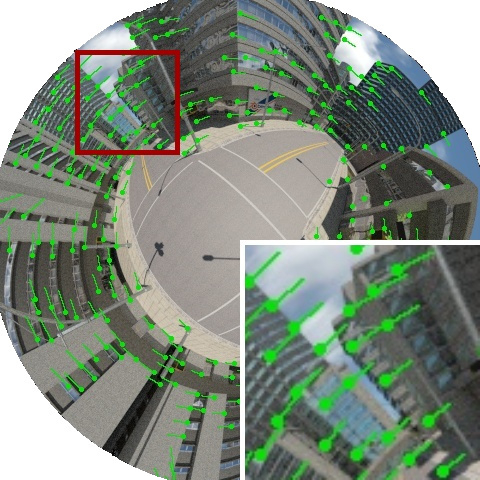
\includegraphics[width=0.65\textwidth]{./figures/robot/method_systemstructure_features_frame.jpg}
    \caption{Computed features and optical flow are shown in green.}
    \label{fig:robot_methods_flowchart_enlargement_features}
  \end{subfigure}\\
  \begin{subfigure}[]{\textwidth}
    \centering
    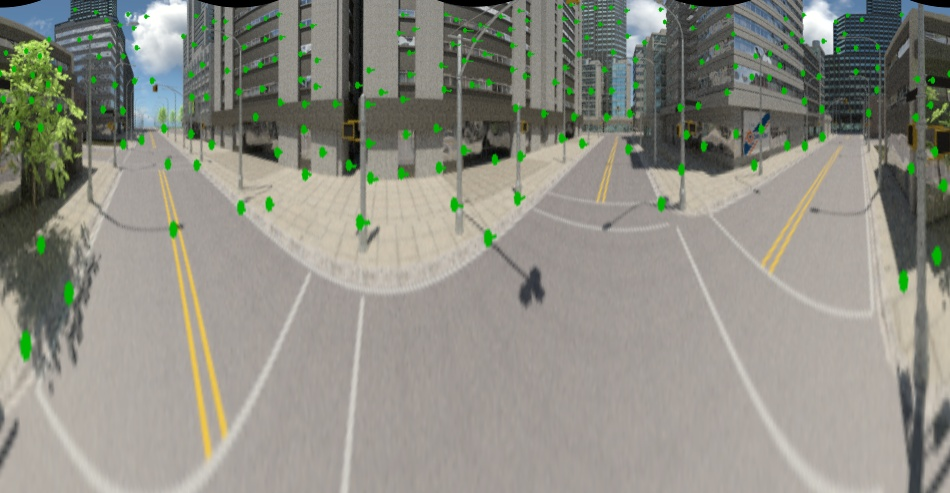
\includegraphics[width=0.9\textwidth]{./figures/robot/method_systemstructure_transform_canyonfeatures.jpg}
    \caption{Transformation from mirror to robot coordinate system (not all features shown for visualization purposes).}
    \label{fig:robot_method_systemstructure_enlargement_transform}
  \end{subfigure}
  \caption{Enlargement of example frames b) and c) from \figref{fig:perception_methods_visualodometryalgorithm_flowchart}.}
  \label{fig:robot_methods_flowchart_enlargement}
\end{figure}





\subsubsection{Camera Calibration}

In order to compute motion from camera images, the intrinsic parameters of the camera system need to be known.
This can be done by utilizing a model for catadioptric camera systems as proposed by~\cite{scaramuzza2006flexible}.
For that case, the projection equation for image points $(u,v)^T$ is given by
\begin{equation}
 \lambda
 \begin{bmatrix}
  u\\
  v\\
  a_0+a_1p+\cdots+a_{n}p^{n}
 \end{bmatrix} =
 \begin{bmatrix}
  x\\
  y\\
  z
 \end{bmatrix} \text{,}
\end{equation}
with \[p = \sqrt {u^2+v^2}\] and $a_0$, $a_1$, $\dots$, $a_n$ being the intrinsic calibrated parameters depending on the camera system. 
This model assumes that camera and mirror are well aligned.
Since the camera and mirror frame is rigid, the assumption holds in all tested use cases.
However, if this were not the case, an affine transformation on the computed points is needed.
If all parameters of the camera and the used mirror in a catadioptric system are known, one can calculate point projections as follows.





\subsubsection{Transformations between image and world coordinates}

% The prime collides with the vector arrow in $\vec o'$. We adjust the spacing globally.
\let\originalprime\prime
\renewcommand{\prime}{\,\originalprime}
\newcommand{\atanii}{\ensuremath{\mathrm{atan2}}}

In the following, the transformations $T_H$ from image space to the external frame of reference and their inverse $T_H^{-1}$ are derived.
Object positions in image space are denoted using 2d coordinates $\vec o' = ( o'_x, o'_y)^T$ in cartesian or polar coordinates $( \rho, \phi )^T$.
Their counterparts in the external frame of reference are denoted as $\vec o \R3$.
The robot's pose in the external frame of reference is determined by its position $\vec c$ and orientation $\vec q$:
This is the pose of the camera's view as shown in \figref{fig:robot_method_algorithms_mirror_sphere_front} and \figref{fig:robot_method_algorithms_mirror_hyperbola_top}.
Using the real world radius $r$ and radius $r'$ in image space, the reflection's position on the mirror can be computed independently of camera parameters using the scaling factor $s = \,^r\!/_{r'}$.

\begin{figure}
  \centering
  \begin{subfigure}[]{0.3\textwidth}
    \centering
    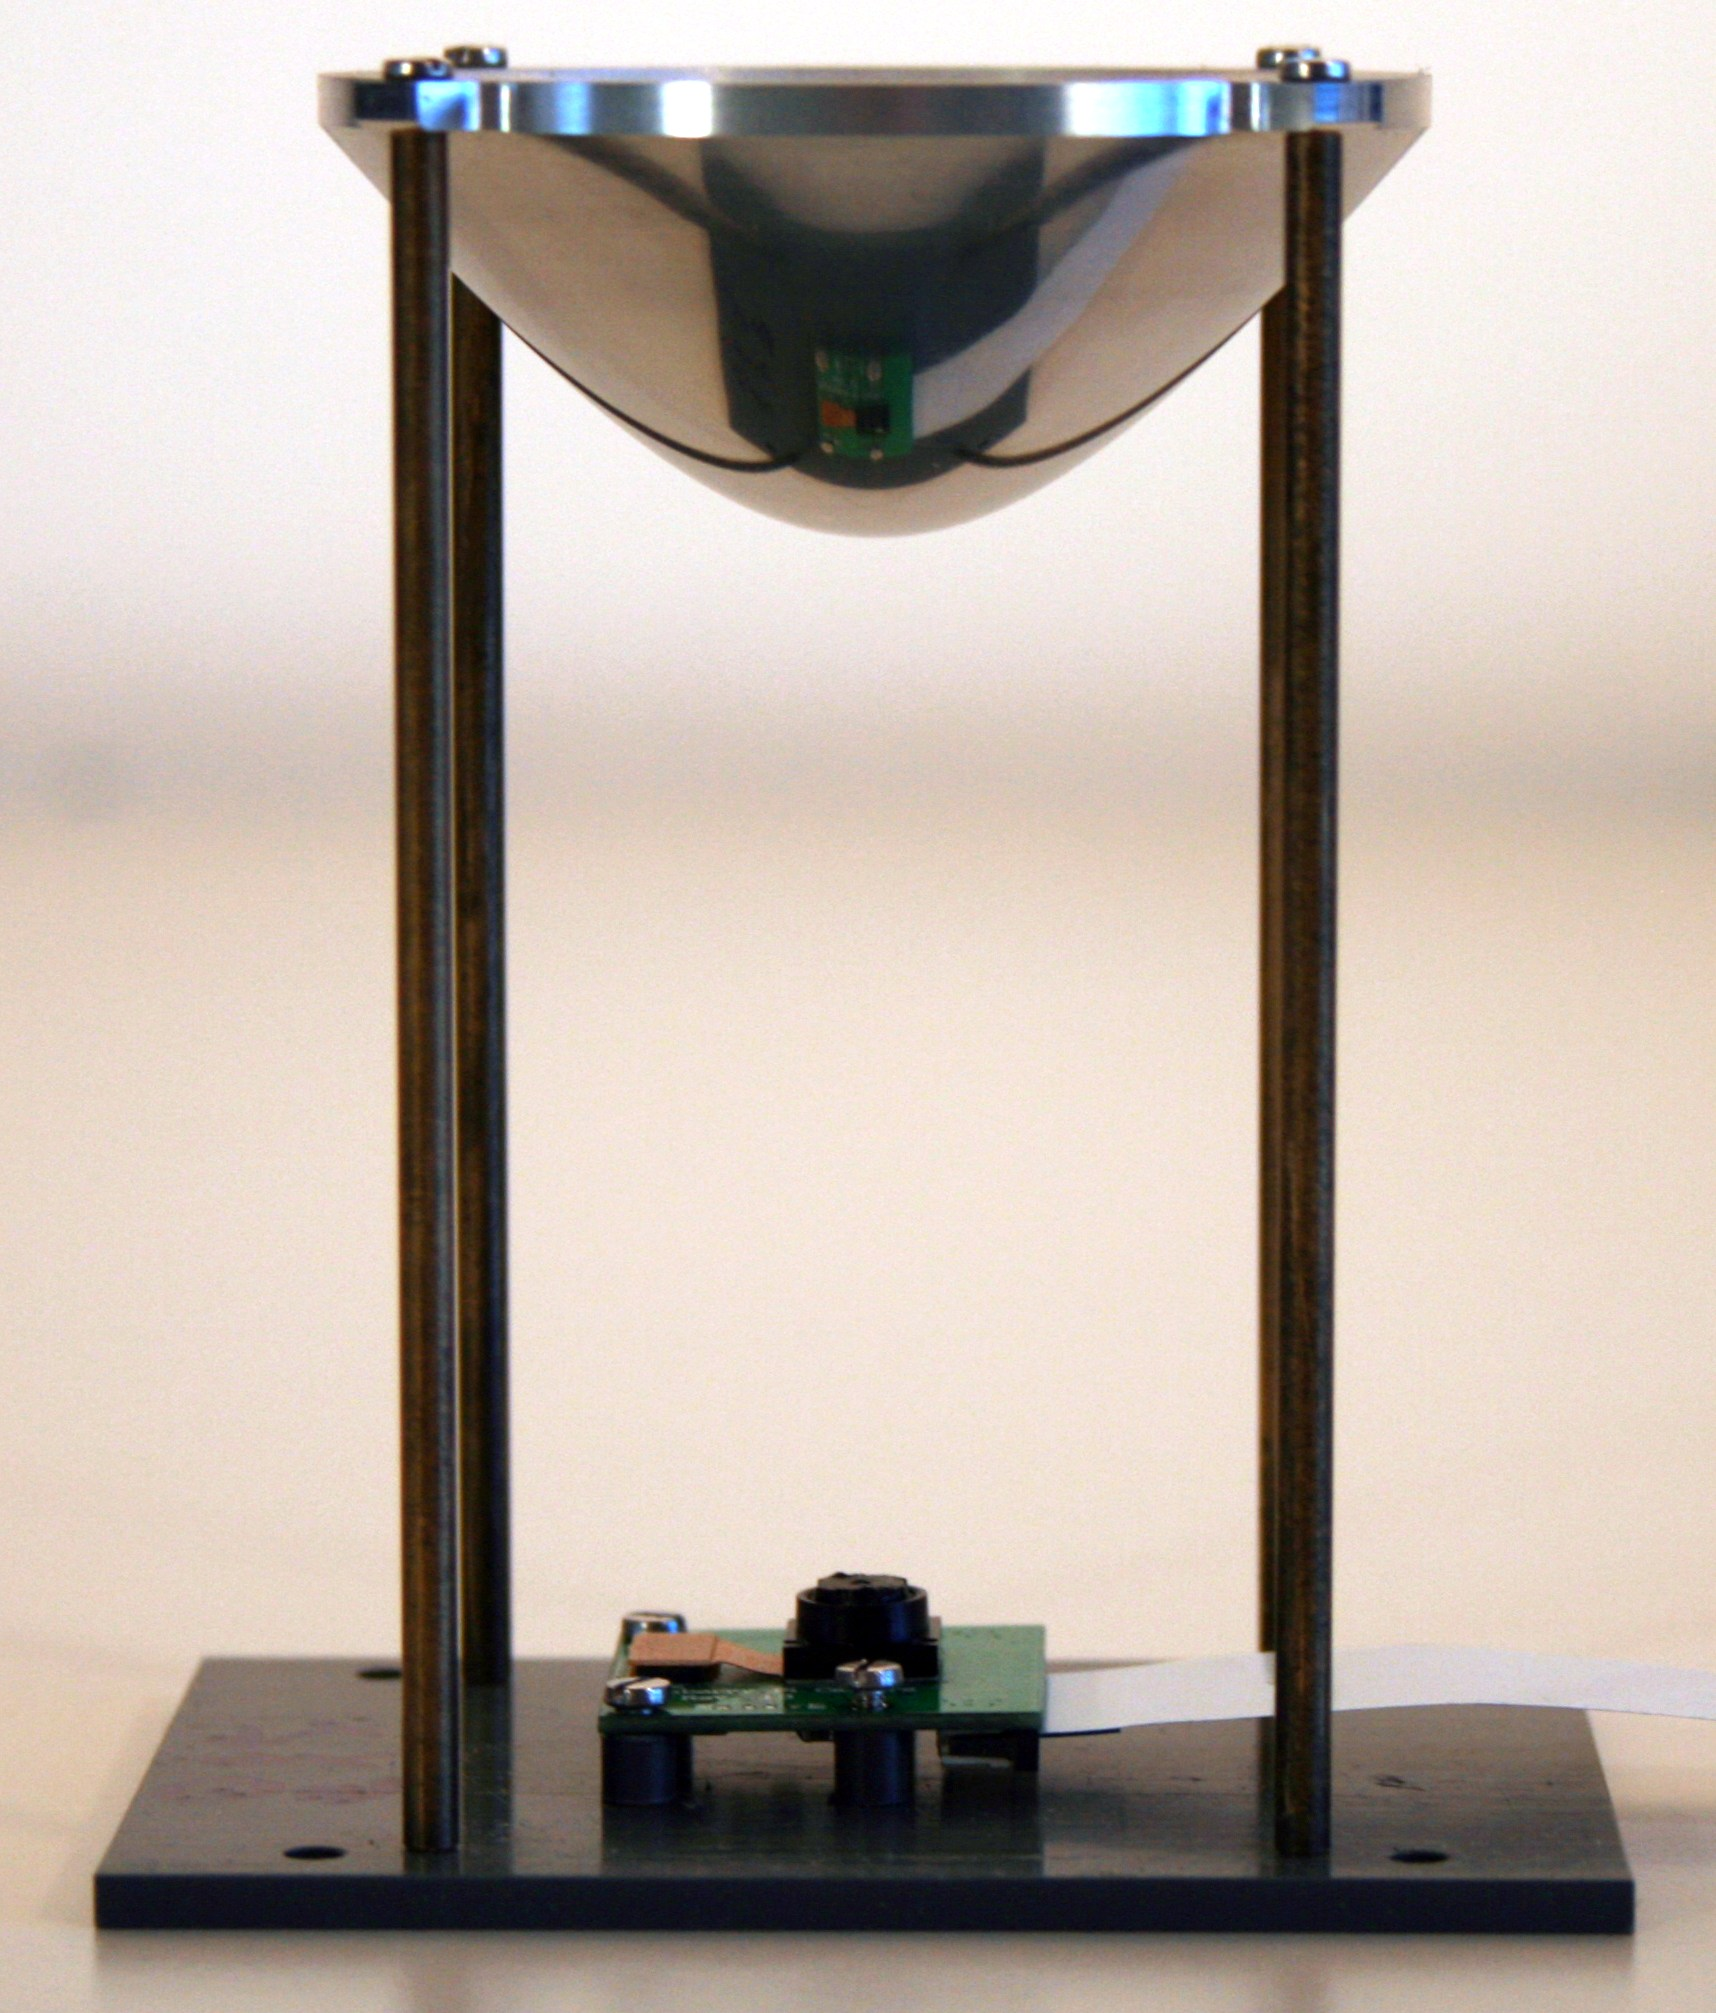
\includegraphics[height=3.55cm]{./figures/robot/photos/mirror.jpg}
    \caption{Photo of the hyperbola mirror.}
    \label{fig:robot_method_algorithms_mirror_hyperbolaphoto}
  \end{subfigure}\hfill
  \begin{subfigure}[]{0.3\textwidth}
    \centering
    % Define block styles
\tikzstyle{block} = [draw, rectangle, text centered, text width=10em, minimum height=0.5em, rounded corners=true]
\tikzstyle{background} = [draw, rectangle, text centered, text width=3.5cm, minimum height=3.5cm, color=white]
\tikzstyle{arrowtext} = [text width=4em, text centered]
\tikzstyle{arrow} = [draw, -latex]

\definecolor{red1}{RGB}{160,0,0}
\definecolor{green1}{RGB}{0,160,0}
\definecolor{blue1}{RGB}{0,0,160}

\usetikzlibrary{shapes.geometric,arrows,positioning,calc,patterns,angles,quotes}

	      
\begin{tikzpicture}[node distance=4em, auto]
    % Background size
    \node[background] at (0,0.15cm) {};

    % circle
    \draw[red1, fill=red1!20] (0,0) circle (1.4);

    % Draw axis
    \draw [->, dashed] (-1.5,0) |- (1.55,0) node [xshift=0.2em, yshift=-0.6em] {x};
    \draw [->, dashed] (0,-1.5) |- (0,1.55) node [xshift=0.6em, yshift=0.1em] {y};
    \draw [-, dashed] (0.8,0.8) -- (0,0);

    % point
    \draw[fill=red1, color=red1] (0.8,0.8) circle (2pt) node [below, color=black, xshift=0.6em, yshift=0.1cm] {$\vec o'$};

    % sizes
    \path[<->]
        (-1.5,0.0) edge node [xshift=0.5em, yshift=0.75em, anchor=center] {$r'$} (-1.5,1.4)
        (-0.2,0.2) edge node [xshift=0.1em, yshift=0.6em, anchor=center] {$\rho'$} (0.5,0.9);

    % angles
    \draw[black, fill=none, <->] (0.7,0.7) arc (45:0:1) node [xshift=-0.38cm, yshift=0.25cm] {$-\phi$};
\end{tikzpicture}

    \caption{Camera view of the mirror.}
    \label{fig:robot_method_algorithms_mirror_sphere_front}
  \end{subfigure}\hfill
  \begin{subfigure}[]{0.3\textwidth}
    \centering
    % Define block styles
\tikzstyle{block} = [draw, rectangle, text centered, text width=10em, minimum height=0.5em, rounded corners=true]
\tikzstyle{arrowtext} = [text width=4em, text centered]
\tikzstyle{background} = [draw, rectangle, text centered, text width=3.5cm, minimum height=3.5cm, color=white]
\tikzstyle{arrow} = [draw, -latex]

\definecolor{red1}{RGB}{160,0,0}
\definecolor{green1}{RGB}{0,160,0}
\definecolor{blue1}{RGB}{0,0,160}
\definecolor{black}{RGB}{0,0,0}
\definecolor{white}{RGB}{255,255,255}

\usetikzlibrary{shapes.geometric,arrows,positioning}

	      
\begin{tikzpicture}[node distance=4em, auto]
    % Background size
    \node[background] at (0,-1.1cm) {};

    % hyperbola
    \pgfmathsetmacro{\e}{1.1};   % eccentricity
    \pgfmathsetmacro{\a}{1.1};
    \pgfmathsetmacro{\b}{(\a*sqrt((\e)^2-1)} 
    \draw[red1, fill=red1!20, yshift=-2.0cm] plot[domain=-1.2:1.2, rotate=90] ({\a*cosh(\x)},{\b*sinh(\x)});

	\coordinate (m) at (0.4,-0.6);
    \coordinate (o) at (1.3,-0.34);
    \coordinate (c) at (0,-1.37);
    \coordinate (v) at (0,-0.74);
    \coordinate (f) at (0,-2.00);
    \coordinate (cam) at (-0.24,-2.8);

    % Draw axis
    \draw [-, dashed] (0,0) |- (0,-2.8);
    \draw [-, dashed] (-1,0) |- (1,0);
	\draw [-, dashed] (v) -- (m);
	\begin{scope}[rotate around={51:(m)}]
			\draw[-, dashed] (0.4-0.5,-0.6) -- (0.4+0.5,-0.6);
	\end{scope}

    % Mini-Coordinate-System
    \draw [->] (1.0,-2.3) |- (1.3,-2.3) node [xshift=0.2em,yshift=-0.3em,anchor=center] {x};
    \draw [->] (1.0,-2.3) -- (1.0,-2.0) node [xshift=0.4em,yshift=-0.2em,anchor=center] {z};
    \draw [color=black, fill=white] (1.0,-2.3) circle(0.056) node [below] {y};
    \draw [-] (0.96,-2.34) -- (1.04,-2.26);
    \draw [-] (0.96,-2.26) -- (1.04,-2.34);

    % Light
    \draw[-, thick] (m) -- (cam);
    \draw[-, thick] (m) -- (o);

    % camera
    %\draw [-, thick, gray] (-0.5,-2.0)
    %    -- (0.5,-2.0)
    %    -- (0.3,-2.3)
    %    -- (-0.3,-2.3)
    %    -- (-0.5,-2.0);
    \draw [-, thick, gray] (0.4,-2.0) 
        -- (0.4,-2.8)
        -- (-0.4,-2.8)
        -- (-0.4,-2.0)
        -- cycle;

    % point
    \draw[fill=red1, color=red1] (m) circle (2pt) node [below, color=black, xshift=0.3em, yshift=0.1] {}; % was: $\hat{\vec o}$
    \draw[fill=red1, color=red1] (o) circle (2pt) node [below, color=black, xshift=0.3em, yshift=0.1] {$\vec{o}$};
    \draw[fill=red1, color=red1] (c) circle (2pt) node [below, color=black, xshift=-0.5em] {$\vec{c}$};
    \draw[fill=red1, color=red1] (v) circle (2pt) node [above, color=black, xshift=-0.5em] {$\mathcal{F}_1$};
    \draw[fill=red1, color=red1] (f) circle (2pt) node [below, color=black, xshift=0.5em] {$\mathcal{F}_2$};

    % sizes
    \path[<->]
        (-1.0,-0.74) edge node [xshift=-0.75em, anchor=center] {$2\varepsilon$} (-1.0,-2.0)
        (-1.0,-2.0) edge node [xshift=-0.5em, anchor=center] {$f$} (-1.0,-2.8)
        (-0.2,-0.9) edge node [xshift=-0.5em, anchor=center] {$a$} (-0.2,-1.37)
        (0.0,0.2) edge node [yshift=0.5em, anchor=center] {$\rho$} (0.4,0.2)
        (0.0,0.2) edge node [yshift=0.5em, anchor=center] {$r$} (-0.75,0.2)
        (0.6,-1.15) edge node [yshift=-0.5em, anchor=center] {$d$} (1.5,-0.85);
\end{tikzpicture}

    \caption{Side view of hyperbola mirror.}
    \label{fig:robot_method_algorithms_mirror_hyperbola_top}
  \end{subfigure}
  \caption{Sketch of a camera observing an object $\vec{o}$, which appears at position $\vec o'$ in the image plane (b). In Figure (c) the camera is pointed at a hyperbolic mirror.}
  \label{fig:robot_method_algorithms_mirror}
\end{figure}

\newcommand{\Fi}{\ensuremath{\mathcal{F}_1}}
\newcommand{\Fii}{\ensuremath{\mathcal{F}_2}}

The surface of a hyperbolic mirror is defined by
\begin{equation}
  \frac{y^2}{a^2} - \frac{x^2}{b^2} = 1 \quad,~a, b \R{1}
\end{equation}
with the semi-major axis $a$. 
The focal points $\mathcal{F}_{1,2}$ are set apart by \[{2\sqrt{a^2 + b^2} =: 2\epsilon}\] (\figref{fig:robot_method_algorithms_mirror_hyperbola_top}).
The robot's position is defined by the point in the middle of these two focal points.
The camera's focal point coincides with $\Fii$.
With ${\vec e}$ being the unit vector pointing from the reflection on the mirror towards the object's position $\vec o$:

\begin{equation}
  \nonumber
  \vec e_H(\vec o') =
    \frac{\left( s \, \vec o'_x, s \, \vec o'_y, \frac{a}{b} \sqrt{\rho^2 + b^2} - \varepsilon \right)^\intercal}
    {\left| \left( s \, \vec o'_x, s \, \vec o'_y, \frac{a}{b} \sqrt{\rho^2 + b^2} - \varepsilon \right)^\intercal \right|} \quad \text{,}
\end{equation}

the transformation $T_H$ is

\begin{equation}
  \nonumber
  \begin{aligned}
    T_H: & \vec o' \longmapsto \vec o : \\
    \vec o = & \vec c + R(\vec q)
    \left( \begin{array}{c}
             s o'_x\\
             s o'_y\\
             \frac{a}{b} \sqrt{\rho(\vec o')^2 + b^2}
           \end{array} + d \vec e_H(\vec o') \right) \quad \text{.}
    \end{aligned}
\end{equation}

and therefore the object position at a distance $d$ is defined as $\vec o = \vec r + R \left( \hat{\vec o} + \Di \vec e \right)$.
For the inverse transformation in polar coordinates, it can be shown that the radius $\rho'$ is given by

\begin{equation}
  \rho' = \frac{\left( \vec o - \vec c \right)_\rho}{\left( \vec o - \vec c \right)^2_\rho \cdot \varepsilon^2 / b^2 -1}
         \left( \left( \vec o - \vec c \right)_z \varepsilon + a \right) \quad \text{.}
\end{equation}

To simplify these expressions, the rotation matrix $R$ was left out.
Different camera orientations $\vec q$ are accounted for by rotating the vector $\left( \vec o - \vec c \right)$ before calculations.
The corresponding image position is now found as $\vec o' = \left( \rho \cos \phi, \rho \sin \phi \right)^\intercal$.





\subsubsection{Feature Set}

As already mentioned, features are first computed on the raw camera image.
Features are points in an image, which are easy to find, recognize, and track in consecutive frames --- usually areas rich in texture.
Afterwards, the optical flow is computed using these features.
There are numerous publications comparing different feature algorithms --- the most prominent algorithms include FAST~\cite{Rosten2006}, GFTT~\cite{shi1994}, ORB~\cite{rublee2011orb}, SIFT~\cite{lowe1999object}, and SURF~\cite{bay2006}.
Here, FAST is used as it offers a good trade-off between computational complexity and quality of found features~\cite{Elgayar2013175, Heinly2012}.
Then, the optical flow is estimated using a pyramidical implementation of the Lucas-Kanade method~\cite{bouguet2001pyramidal}.





\subsubsection{Motion and Depth Estimation}

Now, one can compute the robot's displacement (translation and rotation) between consecutive frames.
A list of all features for all frames is kept, which means the position of each feature relative to multiple robot positions is available.
This enables the robot to perform triangulation.
While in theory one would get a good estimate, real world experiments show that quite a lot of noise gets introduced.

Estimating the depth for $N$ features adds significant complexity to the problem.
Currently, \gls{ac:evo} tries to estimate the quadrocopter's 6d motion $M$ --- consisting of translation $\Delta \vec r$ and orientation $\Delta \vec q$.
Our problem has now increased to $N + 6$ dimensions.
Changes in the feature set from frame $\vec i_{i, t-1}$ to frame $\vec i_{i, t}$ provide $N$ equations, meaning features need to be tracked for at least $3$ consecutive frames.

\newcommand{\pr}{\ensuremath{{\,p}}}
\paragraph{Computing the feature correspondence}
\begin{enumerate}
  \item Depth $d_{i,t-1}$ and motion $M_{t}$ are initialized using previous data $d_{i,t-2}$ and motion $M_{t-1}$. The camera pose $P_{t-1}$, consisting of position $\vec c_{t-1}$ and rotation $\vec q_{t-1}$, is known.
  \item For every feature $i$, calculate the global position $\vec o_{i,t - 1}$ using the depth $d_{i,t-1}$, the image coordinates $\vec o'_{i,t - 1}$ and the camera pose $P_{t-1}$ using the transformation $T_H$.
  \item Apply the inverse motion to all global positions $\vec o_{i, t-1}$. This results in the predicted global positions $\vec o^\pr_{i, t}$.
  \item Use the inverse transformation $T^{-1}_H$, to compute the predicted image position $\vec{o}'^{p}_{i, t} = T^{-1}_H \left( \vec{o}^\pr_{i, t} \right)$.
  \item Lastly, the environment as well as all global features is considered to be static. Therefore, one may minimize the sum of the squared distances for the last $L$ time steps:
  \[\textrm{SD} \left( d_{i, t}, M \right) = \sum_{i=0}^{N} \sum_{t=-L}^{0} \left\lVert \vec o'_{i,t} - \vec o^{\prime p}_{i,t} \right\rVert^2 .\]
\end{enumerate}

\paragraph{Estimating the depth with the forward estimation}
\begin{enumerate}
  \item Perform step 1. and 2. from the inverse estimation.
  \item The goal is to find the new depth $d_{i, t}$ based on the previous estimate $d_{i, t-1}$.
    %In the pinhole model, the depth is defined as the $y$-component of the difference between the object position $\vec o_i$ and the camera position $\vec c$:
    %${d_{t} = \left( R \left( \Delta \vec{q}_{t} \right) \left( \vec o - \vec c_{t-1} - \Delta \vec c_t \right) \right)_y \, \text{.}}$
    In omnidirectional mirror models, the depth is
    \[{d_{t} = \left\lVert R \left( \Delta \vec{q}_{t} \right) \left( \vec o - \vec c - \Delta \vec c_t \right) - \hat{\vec o}^{\,p} \, \right\rVert \, \text{.}}\]
    The new reflection point $\hat{\vec o}^p$ is calculated with the inverse transformation $T^{-1}_H$.
  \item Compute the new predicted pose $P_{t} = P_{t-1} + M_{t}$.
  \item Compute predicted global positions $\vec o^\pr_{i, t=0}$ for every feature $i$ based on the camera model.
  \item The positions $\vec o_{i, t}$ and $\vec o^\pr_{i, t}$ should be equal for corresponding features $i$. We use this to minimize the sum of the squared distances
\begin{equation}
  \nonumber
  \textrm{SD} \left( d_{i, t}, M \right) = \sum_{i=0}^{N} \sum_{\tau=-L}^{0} \left\lVert \frac{ \vec o_{i,t-\tau} - \vec{o}^\pr_{i, t-\tau}}{d_{i,t-\tau}} \right\rVert^2.
\end{equation}
Now, $d_{i,t}^{-1}$ weights all summands consistently as the position-error scales linearly with $d$.
\end{enumerate}





\subsubsection{Maximum angular resolution}

Given a fixed camera resolution of $\unit[480 \times 480]{px}$ one can now compute the projection of the hyperbola mirror onto the camera. 
It is assumed that the object is at a distance of $\unit[2]{m}$ and five pixels width to separate it from adjacent objects are required. 
After straightforward application of the above formulas, the limit is derived as approximately $1.3\degree$.

\section{Results}
\label{perception_results}

In this section, we will first look at the user controlled parameters, the subwindow size $N$ (\secref{ssec:perception_results_subwindowsize}) and the threshold $\tau$ (\secref{ssec:perception_results_threshold}).
The Gaussian smoothing parameters, which are also hyperparameters, heavily depend on the data type: is the filter too strong, the final image will be blurry; a filter too weak will not smooth enough.
Heuristically a kernel sized $\unit[5]{px}$ and $\sigma = 0.3$ was found to work very well for all images in the data sets.
Afterwards, the proposed filter is compared to the bilateral filter, simple Gaussian kernel, Median filter, and Non-local-means filter. 
Lastly, an analysis of the computational complexity and real-time implementations is performed.

While many other robots perform indoor navigation, only few are able to do so without external computing power: for example~\cite{engel2012accurate, forster2014svo, kerl2013robust, forster2017svo}.
The main requirement for successful employment of \gls{ac:vo} based methods is to obtain high accuracy and robustness given a limited computational budget.
The joint optimization of structure, \ie landmarks, and motion, \ie the robot's pose, is commonly called bundle adjustment~\cite{triggs1999bundle, forster2017svo}.
Thus, to separate problems stemming from \gls{ac:vo} and problems arising from the flight controller, the next section analyzes the proposed algorithm using two simulations and compare results to current state-of-the-art (\secref{ssec:perception_results_visualodometryinsimulation}).

Afterwards, real-world measurements are shown, where \gls{ac:vo} data is fused with \gls{ac:imu} pose information, \secref{ssec:perception_results_externallytrackedindoorflights}.
Here, ground truth is generated via external tracking.
Only short trajectories are used in this section due to camera limitations.
In the next section, long term real world flights are shown (\secref{ssec:perception_results_officeindoorflight}).
Lastly, the \gls{ac:vo} algorithm's time performance is evaluated, please see \secref{ssec:perception_results_timeperformanceofvisualodometryalgorithm}.



\subsection{Effect on denoising of different subwindow sizes}
\label{ssec:perception_results_subwindowsize}

\begin{figure}[]
  \centering
  \begin{subfigure}[]{\textwidth}
    \centering
    \begin{tikzpicture}[gnuplot]
%% generated with GNUPLOT 5.0p1 (Gentoo revision r1) (Lua 5.1; terminal rev. 99, script rev. 100)
%% Tue 07 Feb 2017 11:32:39 AM CET
%\gpfill{rgb color={0.000,0.667,0.000},opacity=0.20} (0.577,0.498)--(5.577,0.498)--(5.577,0.498)--cycle;
%\gpfill{color=gpbgfillcolor} (-3.837,4.754)--(9.992,4.754)--(9.992,5.171)--(-3.837,5.171)--cycle;
\gpcolor{color=gp lt color border}
\node[gp node right] at (-0.838,4.962) {Original Data};
\gpcolor{rgb color={0.667,0.000,0.000}}
\gpsetlinewidth{2.00}
\gpsetpointsize{4.00}
\gppoint{gp mark 2}{(-0.033,4.962)}
\gpcolor{color=gp lt color border}
\node[gp node right] at (3.772,4.962) {Filtered Data};
\gpcolor{rgb color={0.000,0.000,0.667}}
\gppoint{gp mark 1}{(4.577,4.962)}
\gpcolor{color=gp lt color border}
\node[gp node right] at (8.382,4.962) {Threshold $\tau$};
\gpfill{rgb color={0.000,0.667,0.000},opacity=0.20} (8.613,4.858)--(9.762,4.858)--(9.762,5.067)--(8.613,5.067)--cycle;
%% coordinates of the plot area
\gpdefrectangularnode{gp plot 1}{\pgfpoint{0.577cm}{0.498cm}}{\pgfpoint{5.577cm}{4.498cm}}
\end{tikzpicture}
%% gnuplot variables

  \end{subfigure}\vspace{0.25cm}\\
  \begin{subfigure}[]{\textwidth}
    \centering
    \begin{tikzpicture}[gnuplot]
%% generated with GNUPLOT 5.2p2 (Gentoo revision r0) (Lua 5.1; terminal rev. 99, script rev. 102)
%% Thu 28 Jun 2018 01:10:02 PM CEST
\gpcolor{color=gp lt color border}
\gpsetlinetype{gp lt border}
\gpsetdashtype{gp dt solid}
\gpsetlinewidth{1.00}
\draw[gp path] (1.322,1.360)--(1.532,1.360);
\node[gp node right] at (1.322,1.360) {0};
\draw[gp path] (1.322,2.527)--(1.532,2.527);
\node[gp node right] at (1.322,2.527) {10};
\draw[gp path] (1.322,3.693)--(1.532,3.693);
\node[gp node right] at (1.322,3.693) {20};
\draw[gp path] (1.553,1.360)--(1.553,1.634);
\node[gp node center] at (1.553,0.891) {0};
\draw[gp path] (3.860,1.360)--(3.860,1.634);
\node[gp node center] at (3.860,0.891) {10};
\draw[gp path] (6.168,1.360)--(6.168,1.634);
\node[gp node center] at (6.168,0.891) {20};
\draw[gp path] (8.476,1.360)--(8.476,1.634);
\node[gp node center] at (8.476,0.891) {30};
\draw[gp path] (10.784,1.360)--(10.784,1.634);
\node[gp node center] at (10.784,0.891) {40};
\draw[gp path] (13.092,1.360)--(13.092,1.634);
\node[gp node center] at (13.092,0.891) {50};
\draw[gp path] (1.322,4.860)--(1.322,1.360)--(13.322,1.360)--(13.322,4.860)--cycle;
\node[gp node center,rotate=-270] at (0.321,3.110) {grayscale value};
\node[gp node center] at (7.322,0.326) {pixel number};
\gpcolor{rgb color={0.667,0.000,0.000}}
\gpsetlinewidth{2.00}
\gpsetpointsize{4.00}
\gppoint{gp mark 2}{(1.553,1.755)}
\gppoint{gp mark 2}{(1.784,1.919)}
\gppoint{gp mark 2}{(2.015,2.013)}
\gppoint{gp mark 2}{(2.245,1.950)}
\gppoint{gp mark 2}{(2.475,2.097)}
\gppoint{gp mark 2}{(2.707,1.889)}
\gppoint{gp mark 2}{(2.937,2.106)}
\gppoint{gp mark 2}{(3.168,1.846)}
\gppoint{gp mark 2}{(3.399,1.892)}
\gppoint{gp mark 2}{(3.630,2.026)}
\gppoint{gp mark 2}{(3.860,4.277)}
\gppoint{gp mark 2}{(4.091,2.079)}
\gppoint{gp mark 2}{(4.322,1.741)}
\gppoint{gp mark 2}{(4.553,2.077)}
\gppoint{gp mark 2}{(4.783,2.058)}
\gppoint{gp mark 2}{(5.015,2.004)}
\gppoint{gp mark 2}{(5.245,2.020)}
\gppoint{gp mark 2}{(5.476,1.878)}
\gppoint{gp mark 2}{(5.706,2.017)}
\gppoint{gp mark 2}{(5.938,1.875)}
\gppoint{gp mark 2}{(6.168,1.873)}
\gppoint{gp mark 2}{(6.399,1.790)}
\gppoint{gp mark 2}{(6.630,1.969)}
\gppoint{gp mark 2}{(6.861,2.038)}
\gppoint{gp mark 2}{(7.091,2.012)}
\gppoint{gp mark 2}{(7.323,4.492)}
\gppoint{gp mark 2}{(7.553,4.441)}
\gppoint{gp mark 2}{(7.784,4.269)}
\gppoint{gp mark 2}{(8.014,4.353)}
\gppoint{gp mark 2}{(8.246,4.426)}
\gppoint{gp mark 2}{(8.476,4.338)}
\gppoint{gp mark 2}{(8.706,4.073)}
\gppoint{gp mark 2}{(8.938,4.182)}
\gppoint{gp mark 2}{(9.168,4.297)}
\gppoint{gp mark 2}{(9.399,4.163)}
\gppoint{gp mark 2}{(9.629,4.391)}
\gppoint{gp mark 2}{(9.861,4.204)}
\gppoint{gp mark 2}{(10.091,4.249)}
\gppoint{gp mark 2}{(10.322,4.434)}
\gppoint{gp mark 2}{(10.553,4.507)}
\gppoint{gp mark 2}{(10.784,4.350)}
\gppoint{gp mark 2}{(11.014,4.199)}
\gppoint{gp mark 2}{(11.245,4.309)}
\gppoint{gp mark 2}{(11.476,4.134)}
\gppoint{gp mark 2}{(11.707,4.322)}
\gppoint{gp mark 2}{(11.937,4.274)}
\gppoint{gp mark 2}{(12.169,4.389)}
\gppoint{gp mark 2}{(12.399,3.891)}
\gppoint{gp mark 2}{(12.630,4.514)}
\gppoint{gp mark 2}{(12.860,4.300)}
\gpcolor{rgb color={0.000,0.000,0.667}}
\gppoint{gp mark 1}{(1.553,1.878)}
\gppoint{gp mark 1}{(1.784,1.896)}
\gppoint{gp mark 1}{(2.015,1.962)}
\gppoint{gp mark 1}{(2.245,1.985)}
\gppoint{gp mark 1}{(2.475,2.010)}
\gppoint{gp mark 1}{(2.707,1.983)}
\gppoint{gp mark 1}{(2.937,1.978)}
\gppoint{gp mark 1}{(3.168,1.937)}
\gppoint{gp mark 1}{(3.399,1.933)}
\gppoint{gp mark 1}{(3.630,1.921)}
\gppoint{gp mark 1}{(3.860,3.540)}
\gppoint{gp mark 1}{(4.091,1.965)}
\gppoint{gp mark 1}{(4.322,1.960)}
\gppoint{gp mark 1}{(4.553,1.992)}
\gppoint{gp mark 1}{(4.783,2.012)}
\gppoint{gp mark 1}{(5.015,2.013)}
\gppoint{gp mark 1}{(5.245,1.989)}
\gppoint{gp mark 1}{(5.476,1.953)}
\gppoint{gp mark 1}{(5.706,1.939)}
\gppoint{gp mark 1}{(5.938,1.896)}
\gppoint{gp mark 1}{(6.168,1.881)}
\gppoint{gp mark 1}{(6.399,1.883)}
\gppoint{gp mark 1}{(6.630,1.940)}
\gppoint{gp mark 1}{(6.861,1.971)}
\gppoint{gp mark 1}{(7.091,2.006)}
\gppoint{gp mark 1}{(7.323,4.400)}
\gppoint{gp mark 1}{(7.553,4.379)}
\gppoint{gp mark 1}{(7.784,4.367)}
\gppoint{gp mark 1}{(8.014,4.357)}
\gppoint{gp mark 1}{(8.246,4.336)}
\gppoint{gp mark 1}{(8.476,4.287)}
\gppoint{gp mark 1}{(8.706,4.216)}
\gppoint{gp mark 1}{(8.938,4.198)}
\gppoint{gp mark 1}{(9.168,4.230)}
\gppoint{gp mark 1}{(9.399,4.248)}
\gppoint{gp mark 1}{(9.629,4.272)}
\gppoint{gp mark 1}{(9.861,4.275)}
\gppoint{gp mark 1}{(10.091,4.319)}
\gppoint{gp mark 1}{(10.322,4.379)}
\gppoint{gp mark 1}{(10.553,4.394)}
\gppoint{gp mark 1}{(10.784,4.354)}
\gppoint{gp mark 1}{(11.014,4.277)}
\gppoint{gp mark 1}{(11.245,4.252)}
\gppoint{gp mark 1}{(11.476,4.236)}
\gppoint{gp mark 1}{(11.707,4.277)}
\gppoint{gp mark 1}{(11.937,4.252)}
\gppoint{gp mark 1}{(12.169,4.266)}
\gppoint{gp mark 1}{(12.399,4.225)}
\gppoint{gp mark 1}{(12.630,4.365)}
\gppoint{gp mark 1}{(12.860,4.332)}
\gpfill{rgb color={0.000,0.667,0.000},opacity=0.20} (1.322,2.527)--(1.443,2.527)--(1.564,2.527)--(1.685,2.527)%
    --(1.807,2.527)--(1.928,2.527)--(2.049,2.527)--(2.170,2.527)--(2.292,2.527)%
    --(2.413,2.527)--(2.535,2.527)--(2.656,2.527)--(2.777,2.527)--(2.898,2.527)%
    --(3.019,2.527)--(3.140,2.527)--(3.261,2.527)--(3.383,2.527)--(3.504,2.527)%
    --(3.625,2.527)--(3.746,2.527)--(3.867,2.527)--(3.988,2.527)--(4.109,2.527)%
    --(4.232,2.527)--(4.353,2.527)--(4.474,2.527)--(4.595,2.527)--(4.716,2.527)%
    --(4.837,2.527)--(4.959,2.527)--(5.080,2.527)--(5.201,2.527)--(5.322,2.527)%
    --(5.443,2.527)--(5.564,2.527)--(5.685,2.527)--(5.807,2.527)--(5.928,2.527)%
    --(6.049,2.527)--(6.170,2.527)--(6.292,2.527)--(6.413,2.527)--(6.535,2.527)%
    --(6.656,2.527)--(6.777,2.527)--(6.898,2.527)--(7.019,2.527)--(7.140,2.527)%
    --(7.261,2.527)--(7.383,2.527)--(7.504,2.527)--(7.625,2.527)--(7.746,2.527)%
    --(7.867,2.527)--(7.988,2.527)--(8.109,2.527)--(8.232,2.527)--(8.353,2.527)%
    --(8.474,2.527)--(8.595,2.527)--(8.716,2.527)--(8.837,2.527)--(8.959,2.527)%
    --(9.080,2.527)--(9.201,2.527)--(9.322,2.527)--(9.443,2.527)--(9.564,2.527)%
    --(9.685,2.527)--(9.807,2.527)--(9.928,2.527)--(10.049,2.527)--(10.170,2.527)%
    --(10.292,2.527)--(10.413,2.527)--(10.535,2.527)--(10.656,2.527)--(10.777,2.527)%
    --(10.898,2.527)--(11.019,2.527)--(11.140,2.527)--(11.261,2.527)--(11.383,2.527)%
    --(11.504,2.527)--(11.625,2.527)--(11.746,2.527)--(11.867,2.527)--(11.988,2.527)%
    --(12.109,2.527)--(12.232,2.527)--(12.353,2.527)--(12.474,2.527)--(12.595,2.527)%
    --(12.716,2.527)--(12.837,2.527)--(12.959,2.527)--(13.080,2.527)--(13.201,2.527)%
    --(13.322,2.527)--(13.322,1.360)--(1.322,1.360)--cycle;
\gpcolor{color=gp lt color border}
\gpsetlinewidth{1.00}
\draw[gp path] (1.322,4.860)--(1.322,1.360)--(13.322,1.360)--(13.322,4.860)--cycle;
%% coordinates of the plot area
\gpdefrectangularnode{gp plot 1}{\pgfpoint{1.322cm}{1.360cm}}{\pgfpoint{13.322cm}{4.860cm}}
\end{tikzpicture}
%% gnuplot variables

    \caption{Subwindow size of $N = \unit[3]{px}$.}
    \label{fig:sensor_experiments_subwindowsize_3}
  \end{subfigure}\\
  \begin{subfigure}[]{\textwidth}
    \centering
    \begin{tikzpicture}[gnuplot]
%% generated with GNUPLOT 5.2p2 (Gentoo revision r0) (Lua 5.1; terminal rev. 99, script rev. 102)
%% Thu 28 Jun 2018 01:10:02 PM CEST
\gpcolor{color=gp lt color border}
\gpsetlinetype{gp lt border}
\gpsetdashtype{gp dt solid}
\gpsetlinewidth{1.00}
\draw[gp path] (1.322,1.360)--(1.532,1.360);
\node[gp node right] at (1.322,1.360) {0};
\draw[gp path] (1.322,2.527)--(1.532,2.527);
\node[gp node right] at (1.322,2.527) {10};
\draw[gp path] (1.322,3.693)--(1.532,3.693);
\node[gp node right] at (1.322,3.693) {20};
\draw[gp path] (1.553,1.360)--(1.553,1.634);
\node[gp node center] at (1.553,0.891) {0};
\draw[gp path] (3.860,1.360)--(3.860,1.634);
\node[gp node center] at (3.860,0.891) {10};
\draw[gp path] (6.168,1.360)--(6.168,1.634);
\node[gp node center] at (6.168,0.891) {20};
\draw[gp path] (8.476,1.360)--(8.476,1.634);
\node[gp node center] at (8.476,0.891) {30};
\draw[gp path] (10.784,1.360)--(10.784,1.634);
\node[gp node center] at (10.784,0.891) {40};
\draw[gp path] (13.092,1.360)--(13.092,1.634);
\node[gp node center] at (13.092,0.891) {50};
\draw[gp path] (1.322,4.860)--(1.322,1.360)--(13.322,1.360)--(13.322,4.860)--cycle;
\node[gp node center,rotate=-270] at (0.321,3.110) {grayscale value};
\node[gp node center] at (7.322,0.326) {pixel number};
\gpcolor{rgb color={0.667,0.000,0.000}}
\gpsetlinewidth{2.00}
\gpsetpointsize{4.00}
\gppoint{gp mark 2}{(1.553,1.755)}
\gppoint{gp mark 2}{(1.784,1.919)}
\gppoint{gp mark 2}{(2.015,2.013)}
\gppoint{gp mark 2}{(2.245,1.950)}
\gppoint{gp mark 2}{(2.475,2.097)}
\gppoint{gp mark 2}{(2.707,1.889)}
\gppoint{gp mark 2}{(2.937,2.106)}
\gppoint{gp mark 2}{(3.168,1.846)}
\gppoint{gp mark 2}{(3.399,1.892)}
\gppoint{gp mark 2}{(3.630,2.026)}
\gppoint{gp mark 2}{(3.860,4.277)}
\gppoint{gp mark 2}{(4.091,2.079)}
\gppoint{gp mark 2}{(4.322,1.741)}
\gppoint{gp mark 2}{(4.553,2.077)}
\gppoint{gp mark 2}{(4.783,2.058)}
\gppoint{gp mark 2}{(5.015,2.004)}
\gppoint{gp mark 2}{(5.245,2.020)}
\gppoint{gp mark 2}{(5.476,1.878)}
\gppoint{gp mark 2}{(5.706,2.017)}
\gppoint{gp mark 2}{(5.938,1.875)}
\gppoint{gp mark 2}{(6.168,1.873)}
\gppoint{gp mark 2}{(6.399,1.790)}
\gppoint{gp mark 2}{(6.630,1.969)}
\gppoint{gp mark 2}{(6.861,2.038)}
\gppoint{gp mark 2}{(7.091,2.012)}
\gppoint{gp mark 2}{(7.323,4.492)}
\gppoint{gp mark 2}{(7.553,4.441)}
\gppoint{gp mark 2}{(7.784,4.269)}
\gppoint{gp mark 2}{(8.014,4.353)}
\gppoint{gp mark 2}{(8.246,4.426)}
\gppoint{gp mark 2}{(8.476,4.338)}
\gppoint{gp mark 2}{(8.706,4.073)}
\gppoint{gp mark 2}{(8.938,4.182)}
\gppoint{gp mark 2}{(9.168,4.297)}
\gppoint{gp mark 2}{(9.399,4.163)}
\gppoint{gp mark 2}{(9.629,4.391)}
\gppoint{gp mark 2}{(9.861,4.204)}
\gppoint{gp mark 2}{(10.091,4.249)}
\gppoint{gp mark 2}{(10.322,4.434)}
\gppoint{gp mark 2}{(10.553,4.507)}
\gppoint{gp mark 2}{(10.784,4.350)}
\gppoint{gp mark 2}{(11.014,4.199)}
\gppoint{gp mark 2}{(11.245,4.309)}
\gppoint{gp mark 2}{(11.476,4.134)}
\gppoint{gp mark 2}{(11.707,4.322)}
\gppoint{gp mark 2}{(11.937,4.274)}
\gppoint{gp mark 2}{(12.169,4.389)}
\gppoint{gp mark 2}{(12.399,3.891)}
\gppoint{gp mark 2}{(12.630,4.514)}
\gppoint{gp mark 2}{(12.860,4.300)}
\gpcolor{rgb color={0.000,0.000,0.667}}
\gppoint{gp mark 1}{(1.553,1.951)}
\gppoint{gp mark 1}{(1.784,1.954)}
\gppoint{gp mark 1}{(2.015,1.956)}
\gppoint{gp mark 1}{(2.245,1.956)}
\gppoint{gp mark 1}{(2.475,1.957)}
\gppoint{gp mark 1}{(2.707,1.953)}
\gppoint{gp mark 1}{(2.937,1.954)}
\gppoint{gp mark 1}{(3.168,1.950)}
\gppoint{gp mark 1}{(3.399,1.954)}
\gppoint{gp mark 1}{(3.630,1.971)}
\gppoint{gp mark 1}{(3.860,2.227)}
\gppoint{gp mark 1}{(4.091,1.972)}
\gppoint{gp mark 1}{(4.322,1.956)}
\gppoint{gp mark 1}{(4.553,1.959)}
\gppoint{gp mark 1}{(4.783,1.954)}
\gppoint{gp mark 1}{(5.015,1.953)}
\gppoint{gp mark 1}{(5.245,1.950)}
\gppoint{gp mark 1}{(5.476,1.950)}
\gppoint{gp mark 1}{(5.706,1.950)}
\gppoint{gp mark 1}{(5.938,1.950)}
\gppoint{gp mark 1}{(6.168,1.945)}
\gppoint{gp mark 1}{(6.399,1.943)}
\gppoint{gp mark 1}{(6.630,1.942)}
\gppoint{gp mark 1}{(6.861,1.940)}
\gppoint{gp mark 1}{(7.091,1.942)}
\gppoint{gp mark 1}{(7.323,4.318)}
\gppoint{gp mark 1}{(7.553,4.301)}
\gppoint{gp mark 1}{(7.784,4.292)}
\gppoint{gp mark 1}{(8.014,4.287)}
\gppoint{gp mark 1}{(8.246,4.281)}
\gppoint{gp mark 1}{(8.476,4.278)}
\gppoint{gp mark 1}{(8.706,4.277)}
\gppoint{gp mark 1}{(8.938,4.280)}
\gppoint{gp mark 1}{(9.168,4.284)}
\gppoint{gp mark 1}{(9.399,4.283)}
\gppoint{gp mark 1}{(9.629,4.287)}
\gppoint{gp mark 1}{(9.861,4.287)}
\gppoint{gp mark 1}{(10.091,4.292)}
\gppoint{gp mark 1}{(10.322,4.301)}
\gppoint{gp mark 1}{(10.553,4.303)}
\gppoint{gp mark 1}{(10.784,4.301)}
\gppoint{gp mark 1}{(11.014,4.294)}
\gppoint{gp mark 1}{(11.245,4.294)}
\gppoint{gp mark 1}{(11.476,4.284)}
\gppoint{gp mark 1}{(11.707,4.283)}
\gppoint{gp mark 1}{(11.937,4.278)}
\gppoint{gp mark 1}{(12.169,4.275)}
\gppoint{gp mark 1}{(12.399,4.266)}
\gppoint{gp mark 1}{(12.630,4.271)}
\gppoint{gp mark 1}{(12.860,4.269)}
\gpfill{rgb color={0.000,0.667,0.000},opacity=0.20} (1.322,2.527)--(1.443,2.527)--(1.564,2.527)--(1.685,2.527)%
    --(1.807,2.527)--(1.928,2.527)--(2.049,2.527)--(2.170,2.527)--(2.292,2.527)%
    --(2.413,2.527)--(2.535,2.527)--(2.656,2.527)--(2.777,2.527)--(2.898,2.527)%
    --(3.019,2.527)--(3.140,2.527)--(3.261,2.527)--(3.383,2.527)--(3.504,2.527)%
    --(3.625,2.527)--(3.746,2.527)--(3.867,2.527)--(3.988,2.527)--(4.109,2.527)%
    --(4.232,2.527)--(4.353,2.527)--(4.474,2.527)--(4.595,2.527)--(4.716,2.527)%
    --(4.837,2.527)--(4.959,2.527)--(5.080,2.527)--(5.201,2.527)--(5.322,2.527)%
    --(5.443,2.527)--(5.564,2.527)--(5.685,2.527)--(5.807,2.527)--(5.928,2.527)%
    --(6.049,2.527)--(6.170,2.527)--(6.292,2.527)--(6.413,2.527)--(6.535,2.527)%
    --(6.656,2.527)--(6.777,2.527)--(6.898,2.527)--(7.019,2.527)--(7.140,2.527)%
    --(7.261,2.527)--(7.383,2.527)--(7.504,2.527)--(7.625,2.527)--(7.746,2.527)%
    --(7.867,2.527)--(7.988,2.527)--(8.109,2.527)--(8.232,2.527)--(8.353,2.527)%
    --(8.474,2.527)--(8.595,2.527)--(8.716,2.527)--(8.837,2.527)--(8.959,2.527)%
    --(9.080,2.527)--(9.201,2.527)--(9.322,2.527)--(9.443,2.527)--(9.564,2.527)%
    --(9.685,2.527)--(9.807,2.527)--(9.928,2.527)--(10.049,2.527)--(10.170,2.527)%
    --(10.292,2.527)--(10.413,2.527)--(10.535,2.527)--(10.656,2.527)--(10.777,2.527)%
    --(10.898,2.527)--(11.019,2.527)--(11.140,2.527)--(11.261,2.527)--(11.383,2.527)%
    --(11.504,2.527)--(11.625,2.527)--(11.746,2.527)--(11.867,2.527)--(11.988,2.527)%
    --(12.109,2.527)--(12.232,2.527)--(12.353,2.527)--(12.474,2.527)--(12.595,2.527)%
    --(12.716,2.527)--(12.837,2.527)--(12.959,2.527)--(13.080,2.527)--(13.201,2.527)%
    --(13.322,2.527)--(13.322,1.360)--(1.322,1.360)--cycle;
\gpcolor{color=gp lt color border}
\gpsetlinewidth{1.00}
\draw[gp path] (1.322,4.860)--(1.322,1.360)--(13.322,1.360)--(13.322,4.860)--cycle;
%% coordinates of the plot area
\gpdefrectangularnode{gp plot 1}{\pgfpoint{1.322cm}{1.360cm}}{\pgfpoint{13.322cm}{4.860cm}}
\end{tikzpicture}
%% gnuplot variables

    \caption{Subwindow size of $N = \unit[9]{px}$.}
    \label{fig:sensor_experiments_subwindowsize_9}
  \end{subfigure}\\
  \begin{subfigure}[]{\textwidth}
    \centering
    \begin{tikzpicture}[gnuplot]
%% generated with GNUPLOT 5.2p2 (Gentoo revision r0) (Lua 5.1; terminal rev. 99, script rev. 102)
%% Thu 28 Jun 2018 01:10:02 PM CEST
\gpcolor{color=gp lt color border}
\gpsetlinetype{gp lt border}
\gpsetdashtype{gp dt solid}
\gpsetlinewidth{1.00}
\draw[gp path] (1.322,1.360)--(1.532,1.360);
\node[gp node right] at (1.322,1.360) {0};
\draw[gp path] (1.322,2.527)--(1.532,2.527);
\node[gp node right] at (1.322,2.527) {10};
\draw[gp path] (1.322,3.693)--(1.532,3.693);
\node[gp node right] at (1.322,3.693) {20};
\draw[gp path] (1.553,1.360)--(1.553,1.634);
\node[gp node center] at (1.553,0.891) {0};
\draw[gp path] (3.860,1.360)--(3.860,1.634);
\node[gp node center] at (3.860,0.891) {10};
\draw[gp path] (6.168,1.360)--(6.168,1.634);
\node[gp node center] at (6.168,0.891) {20};
\draw[gp path] (8.476,1.360)--(8.476,1.634);
\node[gp node center] at (8.476,0.891) {30};
\draw[gp path] (10.784,1.360)--(10.784,1.634);
\node[gp node center] at (10.784,0.891) {40};
\draw[gp path] (13.092,1.360)--(13.092,1.634);
\node[gp node center] at (13.092,0.891) {50};
\draw[gp path] (1.322,4.860)--(1.322,1.360)--(13.322,1.360)--(13.322,4.860)--cycle;
\node[gp node center,rotate=-270] at (0.321,3.110) {grayscale value};
\node[gp node center] at (7.322,0.326) {pixel number};
\gpcolor{rgb color={0.667,0.000,0.000}}
\gpsetlinewidth{2.00}
\gpsetpointsize{4.00}
\gppoint{gp mark 2}{(1.553,1.755)}
\gppoint{gp mark 2}{(1.784,1.919)}
\gppoint{gp mark 2}{(2.015,2.013)}
\gppoint{gp mark 2}{(2.245,1.950)}
\gppoint{gp mark 2}{(2.475,2.097)}
\gppoint{gp mark 2}{(2.707,1.889)}
\gppoint{gp mark 2}{(2.937,2.106)}
\gppoint{gp mark 2}{(3.168,1.846)}
\gppoint{gp mark 2}{(3.399,1.892)}
\gppoint{gp mark 2}{(3.630,2.026)}
\gppoint{gp mark 2}{(3.860,4.277)}
\gppoint{gp mark 2}{(4.091,2.079)}
\gppoint{gp mark 2}{(4.322,1.741)}
\gppoint{gp mark 2}{(4.553,2.077)}
\gppoint{gp mark 2}{(4.783,2.058)}
\gppoint{gp mark 2}{(5.015,2.004)}
\gppoint{gp mark 2}{(5.245,2.020)}
\gppoint{gp mark 2}{(5.476,1.878)}
\gppoint{gp mark 2}{(5.706,2.017)}
\gppoint{gp mark 2}{(5.938,1.875)}
\gppoint{gp mark 2}{(6.168,1.873)}
\gppoint{gp mark 2}{(6.399,1.790)}
\gppoint{gp mark 2}{(6.630,1.969)}
\gppoint{gp mark 2}{(6.861,2.038)}
\gppoint{gp mark 2}{(7.091,2.012)}
\gppoint{gp mark 2}{(7.323,4.492)}
\gppoint{gp mark 2}{(7.553,4.441)}
\gppoint{gp mark 2}{(7.784,4.269)}
\gppoint{gp mark 2}{(8.014,4.353)}
\gppoint{gp mark 2}{(8.246,4.426)}
\gppoint{gp mark 2}{(8.476,4.338)}
\gppoint{gp mark 2}{(8.706,4.073)}
\gppoint{gp mark 2}{(8.938,4.182)}
\gppoint{gp mark 2}{(9.168,4.297)}
\gppoint{gp mark 2}{(9.399,4.163)}
\gppoint{gp mark 2}{(9.629,4.391)}
\gppoint{gp mark 2}{(9.861,4.204)}
\gppoint{gp mark 2}{(10.091,4.249)}
\gppoint{gp mark 2}{(10.322,4.434)}
\gppoint{gp mark 2}{(10.553,4.507)}
\gppoint{gp mark 2}{(10.784,4.350)}
\gppoint{gp mark 2}{(11.014,4.199)}
\gppoint{gp mark 2}{(11.245,4.309)}
\gppoint{gp mark 2}{(11.476,4.134)}
\gppoint{gp mark 2}{(11.707,4.322)}
\gppoint{gp mark 2}{(11.937,4.274)}
\gppoint{gp mark 2}{(12.169,4.389)}
\gppoint{gp mark 2}{(12.399,3.891)}
\gppoint{gp mark 2}{(12.630,4.514)}
\gppoint{gp mark 2}{(12.860,4.300)}
\gpcolor{rgb color={0.000,0.000,0.667}}
\gppoint{gp mark 1}{(1.553,1.738)}
\gppoint{gp mark 1}{(1.784,1.907)}
\gppoint{gp mark 1}{(2.015,1.998)}
\gppoint{gp mark 1}{(2.245,1.939)}
\gppoint{gp mark 1}{(2.475,2.084)}
\gppoint{gp mark 1}{(2.707,1.883)}
\gppoint{gp mark 1}{(2.937,2.096)}
\gppoint{gp mark 1}{(3.168,1.841)}
\gppoint{gp mark 1}{(3.399,1.886)}
\gppoint{gp mark 1}{(3.630,2.027)}
\gppoint{gp mark 1}{(3.860,2.087)}
\gppoint{gp mark 1}{(4.091,2.079)}
\gppoint{gp mark 1}{(4.322,1.739)}
\gppoint{gp mark 1}{(4.553,2.070)}
\gppoint{gp mark 1}{(4.783,2.052)}
\gppoint{gp mark 1}{(5.015,2.000)}
\gppoint{gp mark 1}{(5.245,2.013)}
\gppoint{gp mark 1}{(5.476,1.875)}
\gppoint{gp mark 1}{(5.706,2.010)}
\gppoint{gp mark 1}{(5.938,1.872)}
\gppoint{gp mark 1}{(6.168,1.869)}
\gppoint{gp mark 1}{(6.399,1.788)}
\gppoint{gp mark 1}{(6.630,1.965)}
\gppoint{gp mark 1}{(6.861,2.033)}
\gppoint{gp mark 1}{(7.091,2.017)}
\gppoint{gp mark 1}{(7.323,4.307)}
\gppoint{gp mark 1}{(7.553,4.297)}
\gppoint{gp mark 1}{(7.784,4.287)}
\gppoint{gp mark 1}{(8.014,4.287)}
\gppoint{gp mark 1}{(8.246,4.286)}
\gppoint{gp mark 1}{(8.476,4.283)}
\gppoint{gp mark 1}{(8.706,4.278)}
\gppoint{gp mark 1}{(8.938,4.281)}
\gppoint{gp mark 1}{(9.168,4.284)}
\gppoint{gp mark 1}{(9.399,4.283)}
\gppoint{gp mark 1}{(9.629,4.287)}
\gppoint{gp mark 1}{(9.861,4.286)}
\gppoint{gp mark 1}{(10.091,4.287)}
\gppoint{gp mark 1}{(10.322,4.287)}
\gppoint{gp mark 1}{(10.553,4.287)}
\gppoint{gp mark 1}{(10.784,4.286)}
\gppoint{gp mark 1}{(11.014,4.284)}
\gppoint{gp mark 1}{(11.245,4.286)}
\gppoint{gp mark 1}{(11.476,4.284)}
\gppoint{gp mark 1}{(11.707,4.286)}
\gppoint{gp mark 1}{(11.937,4.286)}
\gppoint{gp mark 1}{(12.169,4.286)}
\gppoint{gp mark 1}{(12.399,4.284)}
\gppoint{gp mark 1}{(12.630,4.286)}
\gppoint{gp mark 1}{(12.860,4.286)}
\gpfill{rgb color={0.000,0.667,0.000},opacity=0.20} (1.322,2.527)--(1.443,2.527)--(1.564,2.527)--(1.685,2.527)%
    --(1.807,2.527)--(1.928,2.527)--(2.049,2.527)--(2.170,2.527)--(2.292,2.527)%
    --(2.413,2.527)--(2.535,2.527)--(2.656,2.527)--(2.777,2.527)--(2.898,2.527)%
    --(3.019,2.527)--(3.140,2.527)--(3.261,2.527)--(3.383,2.527)--(3.504,2.527)%
    --(3.625,2.527)--(3.746,2.527)--(3.867,2.527)--(3.988,2.527)--(4.109,2.527)%
    --(4.232,2.527)--(4.353,2.527)--(4.474,2.527)--(4.595,2.527)--(4.716,2.527)%
    --(4.837,2.527)--(4.959,2.527)--(5.080,2.527)--(5.201,2.527)--(5.322,2.527)%
    --(5.443,2.527)--(5.564,2.527)--(5.685,2.527)--(5.807,2.527)--(5.928,2.527)%
    --(6.049,2.527)--(6.170,2.527)--(6.292,2.527)--(6.413,2.527)--(6.535,2.527)%
    --(6.656,2.527)--(6.777,2.527)--(6.898,2.527)--(7.019,2.527)--(7.140,2.527)%
    --(7.261,2.527)--(7.383,2.527)--(7.504,2.527)--(7.625,2.527)--(7.746,2.527)%
    --(7.867,2.527)--(7.988,2.527)--(8.109,2.527)--(8.232,2.527)--(8.353,2.527)%
    --(8.474,2.527)--(8.595,2.527)--(8.716,2.527)--(8.837,2.527)--(8.959,2.527)%
    --(9.080,2.527)--(9.201,2.527)--(9.322,2.527)--(9.443,2.527)--(9.564,2.527)%
    --(9.685,2.527)--(9.807,2.527)--(9.928,2.527)--(10.049,2.527)--(10.170,2.527)%
    --(10.292,2.527)--(10.413,2.527)--(10.535,2.527)--(10.656,2.527)--(10.777,2.527)%
    --(10.898,2.527)--(11.019,2.527)--(11.140,2.527)--(11.261,2.527)--(11.383,2.527)%
    --(11.504,2.527)--(11.625,2.527)--(11.746,2.527)--(11.867,2.527)--(11.988,2.527)%
    --(12.109,2.527)--(12.232,2.527)--(12.353,2.527)--(12.474,2.527)--(12.595,2.527)%
    --(12.716,2.527)--(12.837,2.527)--(12.959,2.527)--(13.080,2.527)--(13.201,2.527)%
    --(13.322,2.527)--(13.322,1.360)--(1.322,1.360)--cycle;
\gpcolor{color=gp lt color border}
\gpsetlinewidth{1.00}
\draw[gp path] (1.322,4.860)--(1.322,1.360)--(13.322,1.360)--(13.322,4.860)--cycle;
%% coordinates of the plot area
\gpdefrectangularnode{gp plot 1}{\pgfpoint{1.322cm}{1.360cm}}{\pgfpoint{13.322cm}{4.860cm}}
\end{tikzpicture}
%% gnuplot variables

    \caption{Subwindow size of $N = \unit[29]{px}$.}
    \label{fig:sensor_experiments_subwindowsize_29}
  \end{subfigure}
  \caption{Shown is the effect of different subwindow sizes on one data set: A one dimensional grayscale image containing a color edge at pixel 25 and one outlier at pixel 10. Detailed explanations are shown in text, see~\secref{ssec:perception_results_subwindowsize}.}
  \label{fig:sensor_experiments_subwindowsize}
\end{figure}

First, we will have a look at the effect of the most important user controlled parameter: the size of the subwindow $N$. 
Since each pixel is $N$ times checked, the computational complexity increases linearly with $N$. 
This parameter also controls the amount of noise, which is either classified as noise or color edge. 
In \figref{fig:sensor_experiments_subwindowsize} a one dimensional grayscale image is shown.
It contains a color edge at pixel 25 and one outlier at pixel 10.
It is filtered using three different subwindow sizes $N = \unit[3,9,15]{px}$ and for each size the color edge is preserved. 
For $N = \unit[3]{px}$, \figref{fig:sensor_experiments_subwindowsize_3},  the filter follows the data more closely; this also means that an outlier, as shown in pixel 10 in the data sample, has a greater influence on the filtered data. 
For a subwindow size of $N = \unit[9]{px}$, see \figref{fig:sensor_experiments_subwindowsize_9}, the data is more heavily smoothed and the outlier is almost not visible in the filtered data. 
In \figref{fig:sensor_experiments_subwindowsize_29} a subwindow size of $N = \unit[29]{px}$ was chosen. 
Since the color edge begins at pixel 26, it will be present in almost all subwindows due to the periodic boundary conditions. 
On the left side however, the outlier increases the mean pixelwise distance, such that these pixels are always detected as ``containing a color edge'' and are not smoothed at all.
Only the right side, which does not contain the artificial outlier, is smoothed.

Thus, the subwindow controls the spatial size of a color edge to be detected.





\subsection{Effect on denoising of different thresholds $\tau$}
\label{ssec:perception_results_threshold}

Next, we will analyze the effect of the threshold $\tau$, this is depicted in \figref{fig:sensor_experiments_threshold}. 
As shown in \secref{ssec:perception_methods_noiseandoutlierdetection}, $\tau$ controls the maximum step size for detecting noise and color edges. 
In \figref{fig:sensor_experiments_threshold_10} a threshold of $\tau = 10$ is used, which is small enough to detect the color step and smooth the outlier. 
A larger threshold of $\tau = 15$, used in \figref{fig:sensor_experiments_threshold_15}, already introduces some smoothing at the color edge. 
Please also note, that the outlier pixel at position 10 is not any more detected as noise; instead it begins to affect the smoothing of its neighboring pixels. 
A large threshold of $\tau = 30$ can be seen in \figref{fig:sensor_experiments_threshold_30}; 30 is by far bigger than any data point and consequently everything will be smoothed. 
The color edge is not preserved any more.

Thus, the threshold $\tau$ controls the maximum height of a color edge to be detected.

\begin{figure}[]
  \centering
  \begin{subfigure}[]{\textwidth}
    \centering
    \begin{tikzpicture}[gnuplot]
%% generated with GNUPLOT 5.0p1 (Gentoo revision r1) (Lua 5.1; terminal rev. 99, script rev. 100)
%% Tue 07 Feb 2017 11:32:39 AM CET
%\gpfill{rgb color={0.000,0.667,0.000},opacity=0.20} (0.577,0.498)--(5.577,0.498)--(5.577,0.498)--cycle;
%\gpfill{color=gpbgfillcolor} (-3.837,4.754)--(9.992,4.754)--(9.992,5.171)--(-3.837,5.171)--cycle;
\gpcolor{color=gp lt color border}
\node[gp node right] at (-0.838,4.962) {Original Data};
\gpcolor{rgb color={0.667,0.000,0.000}}
\gpsetlinewidth{2.00}
\gpsetpointsize{4.00}
\gppoint{gp mark 2}{(-0.033,4.962)}
\gpcolor{color=gp lt color border}
\node[gp node right] at (3.772,4.962) {Filtered Data};
\gpcolor{rgb color={0.000,0.000,0.667}}
\gppoint{gp mark 1}{(4.577,4.962)}
\gpcolor{color=gp lt color border}
\node[gp node right] at (8.382,4.962) {Threshold $\tau$};
\gpfill{rgb color={0.000,0.667,0.000},opacity=0.20} (8.613,4.858)--(9.762,4.858)--(9.762,5.067)--(8.613,5.067)--cycle;
%% coordinates of the plot area
\gpdefrectangularnode{gp plot 1}{\pgfpoint{0.577cm}{0.498cm}}{\pgfpoint{5.577cm}{4.498cm}}
\end{tikzpicture}
%% gnuplot variables

  \end{subfigure}\vspace{0.25cm}\\
  \begin{subfigure}[]{\textwidth}
    \centering
    \begin{tikzpicture}[gnuplot]
%% generated with GNUPLOT 5.2p2 (Gentoo revision r0) (Lua 5.1; terminal rev. 99, script rev. 102)
%% Thu 28 Jun 2018 01:12:07 PM CEST
\gpcolor{color=gp lt color border}
\gpsetlinetype{gp lt border}
\gpsetdashtype{gp dt solid}
\gpsetlinewidth{1.00}
\draw[gp path] (1.322,1.360)--(1.532,1.360);
\node[gp node right] at (1.322,1.360) {0};
\draw[gp path] (1.322,2.527)--(1.532,2.527);
\node[gp node right] at (1.322,2.527) {10};
\draw[gp path] (1.322,3.693)--(1.532,3.693);
\node[gp node right] at (1.322,3.693) {20};
\draw[gp path] (1.553,1.360)--(1.553,1.634);
\node[gp node center] at (1.553,0.891) {0};
\draw[gp path] (3.860,1.360)--(3.860,1.634);
\node[gp node center] at (3.860,0.891) {10};
\draw[gp path] (6.168,1.360)--(6.168,1.634);
\node[gp node center] at (6.168,0.891) {20};
\draw[gp path] (8.476,1.360)--(8.476,1.634);
\node[gp node center] at (8.476,0.891) {30};
\draw[gp path] (10.784,1.360)--(10.784,1.634);
\node[gp node center] at (10.784,0.891) {40};
\draw[gp path] (13.092,1.360)--(13.092,1.634);
\node[gp node center] at (13.092,0.891) {50};
\draw[gp path] (1.322,4.860)--(1.322,1.360)--(13.322,1.360)--(13.322,4.860)--cycle;
\node[gp node center,rotate=-270] at (0.321,3.110) {grayscale value};
\node[gp node center] at (7.322,0.326) {pixel number};
\gpcolor{rgb color={0.667,0.000,0.000}}
\gpsetlinewidth{2.00}
\gpsetpointsize{4.00}
\gppoint{gp mark 2}{(1.553,1.755)}
\gppoint{gp mark 2}{(1.784,1.919)}
\gppoint{gp mark 2}{(2.015,2.013)}
\gppoint{gp mark 2}{(2.245,1.950)}
\gppoint{gp mark 2}{(2.475,2.097)}
\gppoint{gp mark 2}{(2.707,1.889)}
\gppoint{gp mark 2}{(2.937,2.106)}
\gppoint{gp mark 2}{(3.168,1.846)}
\gppoint{gp mark 2}{(3.399,1.892)}
\gppoint{gp mark 2}{(3.630,2.026)}
\gppoint{gp mark 2}{(3.860,4.277)}
\gppoint{gp mark 2}{(4.091,2.079)}
\gppoint{gp mark 2}{(4.322,1.741)}
\gppoint{gp mark 2}{(4.553,2.077)}
\gppoint{gp mark 2}{(4.783,2.058)}
\gppoint{gp mark 2}{(5.015,2.004)}
\gppoint{gp mark 2}{(5.245,2.020)}
\gppoint{gp mark 2}{(5.476,1.878)}
\gppoint{gp mark 2}{(5.706,2.017)}
\gppoint{gp mark 2}{(5.938,1.875)}
\gppoint{gp mark 2}{(6.168,1.873)}
\gppoint{gp mark 2}{(6.399,1.790)}
\gppoint{gp mark 2}{(6.630,1.969)}
\gppoint{gp mark 2}{(6.861,2.038)}
\gppoint{gp mark 2}{(7.091,2.012)}
\gppoint{gp mark 2}{(7.323,4.492)}
\gppoint{gp mark 2}{(7.553,4.441)}
\gppoint{gp mark 2}{(7.784,4.269)}
\gppoint{gp mark 2}{(8.014,4.353)}
\gppoint{gp mark 2}{(8.246,4.426)}
\gppoint{gp mark 2}{(8.476,4.338)}
\gppoint{gp mark 2}{(8.706,4.073)}
\gppoint{gp mark 2}{(8.938,4.182)}
\gppoint{gp mark 2}{(9.168,4.297)}
\gppoint{gp mark 2}{(9.399,4.163)}
\gppoint{gp mark 2}{(9.629,4.391)}
\gppoint{gp mark 2}{(9.861,4.204)}
\gppoint{gp mark 2}{(10.091,4.249)}
\gppoint{gp mark 2}{(10.322,4.434)}
\gppoint{gp mark 2}{(10.553,4.507)}
\gppoint{gp mark 2}{(10.784,4.350)}
\gppoint{gp mark 2}{(11.014,4.199)}
\gppoint{gp mark 2}{(11.245,4.309)}
\gppoint{gp mark 2}{(11.476,4.134)}
\gppoint{gp mark 2}{(11.707,4.322)}
\gppoint{gp mark 2}{(11.937,4.274)}
\gppoint{gp mark 2}{(12.169,4.389)}
\gppoint{gp mark 2}{(12.399,3.891)}
\gppoint{gp mark 2}{(12.630,4.514)}
\gppoint{gp mark 2}{(12.860,4.300)}
\gpcolor{rgb color={0.000,0.000,0.667}}
\gppoint{gp mark 1}{(1.553,1.951)}
\gppoint{gp mark 1}{(1.784,1.954)}
\gppoint{gp mark 1}{(2.015,1.956)}
\gppoint{gp mark 1}{(2.245,1.956)}
\gppoint{gp mark 1}{(2.475,1.957)}
\gppoint{gp mark 1}{(2.707,1.953)}
\gppoint{gp mark 1}{(2.937,1.954)}
\gppoint{gp mark 1}{(3.168,1.950)}
\gppoint{gp mark 1}{(3.399,1.954)}
\gppoint{gp mark 1}{(3.630,1.971)}
\gppoint{gp mark 1}{(3.860,2.227)}
\gppoint{gp mark 1}{(4.091,1.972)}
\gppoint{gp mark 1}{(4.322,1.956)}
\gppoint{gp mark 1}{(4.553,1.959)}
\gppoint{gp mark 1}{(4.783,1.954)}
\gppoint{gp mark 1}{(5.015,1.953)}
\gppoint{gp mark 1}{(5.245,1.950)}
\gppoint{gp mark 1}{(5.476,1.950)}
\gppoint{gp mark 1}{(5.706,1.950)}
\gppoint{gp mark 1}{(5.938,1.950)}
\gppoint{gp mark 1}{(6.168,1.945)}
\gppoint{gp mark 1}{(6.399,1.943)}
\gppoint{gp mark 1}{(6.630,1.942)}
\gppoint{gp mark 1}{(6.861,1.940)}
\gppoint{gp mark 1}{(7.091,1.942)}
\gppoint{gp mark 1}{(7.323,4.318)}
\gppoint{gp mark 1}{(7.553,4.301)}
\gppoint{gp mark 1}{(7.784,4.292)}
\gppoint{gp mark 1}{(8.014,4.287)}
\gppoint{gp mark 1}{(8.246,4.281)}
\gppoint{gp mark 1}{(8.476,4.278)}
\gppoint{gp mark 1}{(8.706,4.277)}
\gppoint{gp mark 1}{(8.938,4.280)}
\gppoint{gp mark 1}{(9.168,4.284)}
\gppoint{gp mark 1}{(9.399,4.283)}
\gppoint{gp mark 1}{(9.629,4.287)}
\gppoint{gp mark 1}{(9.861,4.287)}
\gppoint{gp mark 1}{(10.091,4.292)}
\gppoint{gp mark 1}{(10.322,4.301)}
\gppoint{gp mark 1}{(10.553,4.303)}
\gppoint{gp mark 1}{(10.784,4.301)}
\gppoint{gp mark 1}{(11.014,4.294)}
\gppoint{gp mark 1}{(11.245,4.294)}
\gppoint{gp mark 1}{(11.476,4.284)}
\gppoint{gp mark 1}{(11.707,4.283)}
\gppoint{gp mark 1}{(11.937,4.278)}
\gppoint{gp mark 1}{(12.169,4.275)}
\gppoint{gp mark 1}{(12.399,4.266)}
\gppoint{gp mark 1}{(12.630,4.271)}
\gppoint{gp mark 1}{(12.860,4.269)}
\gpfill{rgb color={0.000,0.667,0.000},opacity=0.20} (1.322,2.527)--(1.443,2.527)--(1.564,2.527)--(1.685,2.527)%
    --(1.807,2.527)--(1.928,2.527)--(2.049,2.527)--(2.170,2.527)--(2.292,2.527)%
    --(2.413,2.527)--(2.535,2.527)--(2.656,2.527)--(2.777,2.527)--(2.898,2.527)%
    --(3.019,2.527)--(3.140,2.527)--(3.261,2.527)--(3.383,2.527)--(3.504,2.527)%
    --(3.625,2.527)--(3.746,2.527)--(3.867,2.527)--(3.988,2.527)--(4.109,2.527)%
    --(4.232,2.527)--(4.353,2.527)--(4.474,2.527)--(4.595,2.527)--(4.716,2.527)%
    --(4.837,2.527)--(4.959,2.527)--(5.080,2.527)--(5.201,2.527)--(5.322,2.527)%
    --(5.443,2.527)--(5.564,2.527)--(5.685,2.527)--(5.807,2.527)--(5.928,2.527)%
    --(6.049,2.527)--(6.170,2.527)--(6.292,2.527)--(6.413,2.527)--(6.535,2.527)%
    --(6.656,2.527)--(6.777,2.527)--(6.898,2.527)--(7.019,2.527)--(7.140,2.527)%
    --(7.261,2.527)--(7.383,2.527)--(7.504,2.527)--(7.625,2.527)--(7.746,2.527)%
    --(7.867,2.527)--(7.988,2.527)--(8.109,2.527)--(8.232,2.527)--(8.353,2.527)%
    --(8.474,2.527)--(8.595,2.527)--(8.716,2.527)--(8.837,2.527)--(8.959,2.527)%
    --(9.080,2.527)--(9.201,2.527)--(9.322,2.527)--(9.443,2.527)--(9.564,2.527)%
    --(9.685,2.527)--(9.807,2.527)--(9.928,2.527)--(10.049,2.527)--(10.170,2.527)%
    --(10.292,2.527)--(10.413,2.527)--(10.535,2.527)--(10.656,2.527)--(10.777,2.527)%
    --(10.898,2.527)--(11.019,2.527)--(11.140,2.527)--(11.261,2.527)--(11.383,2.527)%
    --(11.504,2.527)--(11.625,2.527)--(11.746,2.527)--(11.867,2.527)--(11.988,2.527)%
    --(12.109,2.527)--(12.232,2.527)--(12.353,2.527)--(12.474,2.527)--(12.595,2.527)%
    --(12.716,2.527)--(12.837,2.527)--(12.959,2.527)--(13.080,2.527)--(13.201,2.527)%
    --(13.322,2.527)--(13.322,1.360)--(1.322,1.360)--cycle;
\gpcolor{color=gp lt color border}
\gpsetlinewidth{1.00}
\draw[gp path] (1.322,4.860)--(1.322,1.360)--(13.322,1.360)--(13.322,4.860)--cycle;
%% coordinates of the plot area
\gpdefrectangularnode{gp plot 1}{\pgfpoint{1.322cm}{1.360cm}}{\pgfpoint{13.322cm}{4.860cm}}
\end{tikzpicture}
%% gnuplot variables

    \caption{Threshold of $\tau = 10$.}
    \label{fig:sensor_experiments_threshold_10}
  \end{subfigure}\\
  \begin{subfigure}[]{\textwidth}
    \centering
    \begin{tikzpicture}[gnuplot]
%% generated with GNUPLOT 5.2p2 (Gentoo revision r0) (Lua 5.1; terminal rev. 99, script rev. 102)
%% Thu 28 Jun 2018 01:12:07 PM CEST
\gpcolor{color=gp lt color border}
\gpsetlinetype{gp lt border}
\gpsetdashtype{gp dt solid}
\gpsetlinewidth{1.00}
\draw[gp path] (1.322,1.360)--(1.532,1.360);
\node[gp node right] at (1.322,1.360) {0};
\draw[gp path] (1.322,2.527)--(1.532,2.527);
\node[gp node right] at (1.322,2.527) {10};
\draw[gp path] (1.322,3.693)--(1.532,3.693);
\node[gp node right] at (1.322,3.693) {20};
\draw[gp path] (1.553,1.360)--(1.553,1.634);
\node[gp node center] at (1.553,0.891) {0};
\draw[gp path] (3.860,1.360)--(3.860,1.634);
\node[gp node center] at (3.860,0.891) {10};
\draw[gp path] (6.168,1.360)--(6.168,1.634);
\node[gp node center] at (6.168,0.891) {20};
\draw[gp path] (8.476,1.360)--(8.476,1.634);
\node[gp node center] at (8.476,0.891) {30};
\draw[gp path] (10.784,1.360)--(10.784,1.634);
\node[gp node center] at (10.784,0.891) {40};
\draw[gp path] (13.092,1.360)--(13.092,1.634);
\node[gp node center] at (13.092,0.891) {50};
\draw[gp path] (1.322,4.860)--(1.322,1.360)--(13.322,1.360)--(13.322,4.860)--cycle;
\node[gp node center,rotate=-270] at (0.321,3.110) {grayscale value};
\node[gp node center] at (7.322,0.326) {pixel number};
\gpcolor{rgb color={0.667,0.000,0.000}}
\gpsetlinewidth{2.00}
\gpsetpointsize{4.00}
\gppoint{gp mark 2}{(1.553,1.755)}
\gppoint{gp mark 2}{(1.784,1.919)}
\gppoint{gp mark 2}{(2.015,2.013)}
\gppoint{gp mark 2}{(2.245,1.950)}
\gppoint{gp mark 2}{(2.475,2.097)}
\gppoint{gp mark 2}{(2.707,1.889)}
\gppoint{gp mark 2}{(2.937,2.106)}
\gppoint{gp mark 2}{(3.168,1.846)}
\gppoint{gp mark 2}{(3.399,1.892)}
\gppoint{gp mark 2}{(3.630,2.026)}
\gppoint{gp mark 2}{(3.860,4.277)}
\gppoint{gp mark 2}{(4.091,2.079)}
\gppoint{gp mark 2}{(4.322,1.741)}
\gppoint{gp mark 2}{(4.553,2.077)}
\gppoint{gp mark 2}{(4.783,2.058)}
\gppoint{gp mark 2}{(5.015,2.004)}
\gppoint{gp mark 2}{(5.245,2.020)}
\gppoint{gp mark 2}{(5.476,1.878)}
\gppoint{gp mark 2}{(5.706,2.017)}
\gppoint{gp mark 2}{(5.938,1.875)}
\gppoint{gp mark 2}{(6.168,1.873)}
\gppoint{gp mark 2}{(6.399,1.790)}
\gppoint{gp mark 2}{(6.630,1.969)}
\gppoint{gp mark 2}{(6.861,2.038)}
\gppoint{gp mark 2}{(7.091,2.012)}
\gppoint{gp mark 2}{(7.323,4.492)}
\gppoint{gp mark 2}{(7.553,4.441)}
\gppoint{gp mark 2}{(7.784,4.269)}
\gppoint{gp mark 2}{(8.014,4.353)}
\gppoint{gp mark 2}{(8.246,4.426)}
\gppoint{gp mark 2}{(8.476,4.338)}
\gppoint{gp mark 2}{(8.706,4.073)}
\gppoint{gp mark 2}{(8.938,4.182)}
\gppoint{gp mark 2}{(9.168,4.297)}
\gppoint{gp mark 2}{(9.399,4.163)}
\gppoint{gp mark 2}{(9.629,4.391)}
\gppoint{gp mark 2}{(9.861,4.204)}
\gppoint{gp mark 2}{(10.091,4.249)}
\gppoint{gp mark 2}{(10.322,4.434)}
\gppoint{gp mark 2}{(10.553,4.507)}
\gppoint{gp mark 2}{(10.784,4.350)}
\gppoint{gp mark 2}{(11.014,4.199)}
\gppoint{gp mark 2}{(11.245,4.309)}
\gppoint{gp mark 2}{(11.476,4.134)}
\gppoint{gp mark 2}{(11.707,4.322)}
\gppoint{gp mark 2}{(11.937,4.274)}
\gppoint{gp mark 2}{(12.169,4.389)}
\gppoint{gp mark 2}{(12.399,3.891)}
\gppoint{gp mark 2}{(12.630,4.514)}
\gppoint{gp mark 2}{(12.860,4.300)}
\gpcolor{rgb color={0.000,0.000,0.667}}
\gppoint{gp mark 1}{(1.553,1.951)}
\gppoint{gp mark 1}{(1.784,1.954)}
\gppoint{gp mark 1}{(2.015,1.956)}
\gppoint{gp mark 1}{(2.245,1.956)}
\gppoint{gp mark 1}{(2.475,1.957)}
\gppoint{gp mark 1}{(2.707,1.953)}
\gppoint{gp mark 1}{(2.937,1.954)}
\gppoint{gp mark 1}{(3.168,1.951)}
\gppoint{gp mark 1}{(3.399,1.956)}
\gppoint{gp mark 1}{(3.630,1.971)}
\gppoint{gp mark 1}{(3.860,2.234)}
\gppoint{gp mark 1}{(4.091,1.972)}
\gppoint{gp mark 1}{(4.322,1.959)}
\gppoint{gp mark 1}{(4.553,1.959)}
\gppoint{gp mark 1}{(4.783,1.954)}
\gppoint{gp mark 1}{(5.015,1.953)}
\gppoint{gp mark 1}{(5.245,1.950)}
\gppoint{gp mark 1}{(5.476,1.950)}
\gppoint{gp mark 1}{(5.706,1.950)}
\gppoint{gp mark 1}{(5.938,1.985)}
\gppoint{gp mark 1}{(6.168,2.010)}
\gppoint{gp mark 1}{(6.399,2.021)}
\gppoint{gp mark 1}{(6.630,2.088)}
\gppoint{gp mark 1}{(6.861,2.195)}
\gppoint{gp mark 1}{(7.091,2.327)}
\gppoint{gp mark 1}{(7.323,4.048)}
\gppoint{gp mark 1}{(7.553,4.131)}
\gppoint{gp mark 1}{(7.784,4.128)}
\gppoint{gp mark 1}{(8.014,4.179)}
\gppoint{gp mark 1}{(8.246,4.213)}
\gppoint{gp mark 1}{(8.476,4.240)}
\gppoint{gp mark 1}{(8.706,4.277)}
\gppoint{gp mark 1}{(8.938,4.281)}
\gppoint{gp mark 1}{(9.168,4.284)}
\gppoint{gp mark 1}{(9.399,4.283)}
\gppoint{gp mark 1}{(9.629,4.287)}
\gppoint{gp mark 1}{(9.861,4.289)}
\gppoint{gp mark 1}{(10.091,4.294)}
\gppoint{gp mark 1}{(10.322,4.301)}
\gppoint{gp mark 1}{(10.553,4.301)}
\gppoint{gp mark 1}{(10.784,4.301)}
\gppoint{gp mark 1}{(11.014,4.294)}
\gppoint{gp mark 1}{(11.245,4.294)}
\gppoint{gp mark 1}{(11.476,4.284)}
\gppoint{gp mark 1}{(11.707,4.283)}
\gppoint{gp mark 1}{(11.937,4.278)}
\gppoint{gp mark 1}{(12.169,4.275)}
\gppoint{gp mark 1}{(12.399,4.268)}
\gppoint{gp mark 1}{(12.630,4.271)}
\gppoint{gp mark 1}{(12.860,4.269)}
\gpfill{rgb color={0.000,0.667,0.000},opacity=0.20} (1.322,3.110)--(1.443,3.110)--(1.564,3.110)--(1.685,3.110)%
    --(1.807,3.110)--(1.928,3.110)--(2.049,3.110)--(2.170,3.110)--(2.292,3.110)%
    --(2.413,3.110)--(2.535,3.110)--(2.656,3.110)--(2.777,3.110)--(2.898,3.110)%
    --(3.019,3.110)--(3.140,3.110)--(3.261,3.110)--(3.383,3.110)--(3.504,3.110)%
    --(3.625,3.110)--(3.746,3.110)--(3.867,3.110)--(3.988,3.110)--(4.109,3.110)%
    --(4.232,3.110)--(4.353,3.110)--(4.474,3.110)--(4.595,3.110)--(4.716,3.110)%
    --(4.837,3.110)--(4.959,3.110)--(5.080,3.110)--(5.201,3.110)--(5.322,3.110)%
    --(5.443,3.110)--(5.564,3.110)--(5.685,3.110)--(5.807,3.110)--(5.928,3.110)%
    --(6.049,3.110)--(6.170,3.110)--(6.292,3.110)--(6.413,3.110)--(6.535,3.110)%
    --(6.656,3.110)--(6.777,3.110)--(6.898,3.110)--(7.019,3.110)--(7.140,3.110)%
    --(7.261,3.110)--(7.383,3.110)--(7.504,3.110)--(7.625,3.110)--(7.746,3.110)%
    --(7.867,3.110)--(7.988,3.110)--(8.109,3.110)--(8.232,3.110)--(8.353,3.110)%
    --(8.474,3.110)--(8.595,3.110)--(8.716,3.110)--(8.837,3.110)--(8.959,3.110)%
    --(9.080,3.110)--(9.201,3.110)--(9.322,3.110)--(9.443,3.110)--(9.564,3.110)%
    --(9.685,3.110)--(9.807,3.110)--(9.928,3.110)--(10.049,3.110)--(10.170,3.110)%
    --(10.292,3.110)--(10.413,3.110)--(10.535,3.110)--(10.656,3.110)--(10.777,3.110)%
    --(10.898,3.110)--(11.019,3.110)--(11.140,3.110)--(11.261,3.110)--(11.383,3.110)%
    --(11.504,3.110)--(11.625,3.110)--(11.746,3.110)--(11.867,3.110)--(11.988,3.110)%
    --(12.109,3.110)--(12.232,3.110)--(12.353,3.110)--(12.474,3.110)--(12.595,3.110)%
    --(12.716,3.110)--(12.837,3.110)--(12.959,3.110)--(13.080,3.110)--(13.201,3.110)%
    --(13.322,3.110)--(13.322,1.360)--(1.322,1.360)--cycle;
\gpcolor{color=gp lt color border}
\gpsetlinewidth{1.00}
\draw[gp path] (1.322,4.860)--(1.322,1.360)--(13.322,1.360)--(13.322,4.860)--cycle;
%% coordinates of the plot area
\gpdefrectangularnode{gp plot 1}{\pgfpoint{1.322cm}{1.360cm}}{\pgfpoint{13.322cm}{4.860cm}}
\end{tikzpicture}
%% gnuplot variables

    \caption{Threshold of $\tau = 15$.}
    \label{fig:sensor_experiments_threshold_15}
  \end{subfigure}\\
  \begin{subfigure}[]{\textwidth}
    \centering
    \begin{tikzpicture}[gnuplot]
%% generated with GNUPLOT 5.2p2 (Gentoo revision r0) (Lua 5.1; terminal rev. 99, script rev. 102)
%% Thu 28 Jun 2018 01:12:07 PM CEST
\gpcolor{color=gp lt color border}
\gpsetlinetype{gp lt border}
\gpsetdashtype{gp dt solid}
\gpsetlinewidth{1.00}
\draw[gp path] (1.322,1.360)--(1.532,1.360);
\node[gp node right] at (1.322,1.360) {0};
\draw[gp path] (1.322,2.527)--(1.532,2.527);
\node[gp node right] at (1.322,2.527) {10};
\draw[gp path] (1.322,3.693)--(1.532,3.693);
\node[gp node right] at (1.322,3.693) {20};
\draw[gp path] (1.553,1.360)--(1.553,1.634);
\node[gp node center] at (1.553,0.891) {0};
\draw[gp path] (3.860,1.360)--(3.860,1.634);
\node[gp node center] at (3.860,0.891) {10};
\draw[gp path] (6.168,1.360)--(6.168,1.634);
\node[gp node center] at (6.168,0.891) {20};
\draw[gp path] (8.476,1.360)--(8.476,1.634);
\node[gp node center] at (8.476,0.891) {30};
\draw[gp path] (10.784,1.360)--(10.784,1.634);
\node[gp node center] at (10.784,0.891) {40};
\draw[gp path] (13.092,1.360)--(13.092,1.634);
\node[gp node center] at (13.092,0.891) {50};
\draw[gp path] (1.322,4.860)--(1.322,1.360)--(13.322,1.360)--(13.322,4.860)--cycle;
\node[gp node center,rotate=-270] at (0.321,3.110) {grayscale value};
\node[gp node center] at (7.322,0.326) {pixel number};
\gpcolor{rgb color={0.667,0.000,0.000}}
\gpsetlinewidth{2.00}
\gpsetpointsize{4.00}
\gppoint{gp mark 2}{(1.553,1.755)}
\gppoint{gp mark 2}{(1.784,1.919)}
\gppoint{gp mark 2}{(2.015,2.013)}
\gppoint{gp mark 2}{(2.245,1.950)}
\gppoint{gp mark 2}{(2.475,2.097)}
\gppoint{gp mark 2}{(2.707,1.889)}
\gppoint{gp mark 2}{(2.937,2.106)}
\gppoint{gp mark 2}{(3.168,1.846)}
\gppoint{gp mark 2}{(3.399,1.892)}
\gppoint{gp mark 2}{(3.630,2.026)}
\gppoint{gp mark 2}{(3.860,4.277)}
\gppoint{gp mark 2}{(4.091,2.079)}
\gppoint{gp mark 2}{(4.322,1.741)}
\gppoint{gp mark 2}{(4.553,2.077)}
\gppoint{gp mark 2}{(4.783,2.058)}
\gppoint{gp mark 2}{(5.015,2.004)}
\gppoint{gp mark 2}{(5.245,2.020)}
\gppoint{gp mark 2}{(5.476,1.878)}
\gppoint{gp mark 2}{(5.706,2.017)}
\gppoint{gp mark 2}{(5.938,1.875)}
\gppoint{gp mark 2}{(6.168,1.873)}
\gppoint{gp mark 2}{(6.399,1.790)}
\gppoint{gp mark 2}{(6.630,1.969)}
\gppoint{gp mark 2}{(6.861,2.038)}
\gppoint{gp mark 2}{(7.091,2.012)}
\gppoint{gp mark 2}{(7.323,4.492)}
\gppoint{gp mark 2}{(7.553,4.441)}
\gppoint{gp mark 2}{(7.784,4.269)}
\gppoint{gp mark 2}{(8.014,4.353)}
\gppoint{gp mark 2}{(8.246,4.426)}
\gppoint{gp mark 2}{(8.476,4.338)}
\gppoint{gp mark 2}{(8.706,4.073)}
\gppoint{gp mark 2}{(8.938,4.182)}
\gppoint{gp mark 2}{(9.168,4.297)}
\gppoint{gp mark 2}{(9.399,4.163)}
\gppoint{gp mark 2}{(9.629,4.391)}
\gppoint{gp mark 2}{(9.861,4.204)}
\gppoint{gp mark 2}{(10.091,4.249)}
\gppoint{gp mark 2}{(10.322,4.434)}
\gppoint{gp mark 2}{(10.553,4.507)}
\gppoint{gp mark 2}{(10.784,4.350)}
\gppoint{gp mark 2}{(11.014,4.199)}
\gppoint{gp mark 2}{(11.245,4.309)}
\gppoint{gp mark 2}{(11.476,4.134)}
\gppoint{gp mark 2}{(11.707,4.322)}
\gppoint{gp mark 2}{(11.937,4.274)}
\gppoint{gp mark 2}{(12.169,4.389)}
\gppoint{gp mark 2}{(12.399,3.891)}
\gppoint{gp mark 2}{(12.630,4.514)}
\gppoint{gp mark 2}{(12.860,4.300)}
\gpcolor{rgb color={0.000,0.000,0.667}}
\gppoint{gp mark 1}{(1.553,1.953)}
\gppoint{gp mark 1}{(1.784,1.954)}
\gppoint{gp mark 1}{(2.015,1.982)}
\gppoint{gp mark 1}{(2.245,2.004)}
\gppoint{gp mark 1}{(2.475,2.039)}
\gppoint{gp mark 1}{(2.707,2.062)}
\gppoint{gp mark 1}{(2.937,2.108)}
\gppoint{gp mark 1}{(3.168,2.125)}
\gppoint{gp mark 1}{(3.399,2.160)}
\gppoint{gp mark 1}{(3.630,2.199)}
\gppoint{gp mark 1}{(3.860,2.231)}
\gppoint{gp mark 1}{(4.091,2.202)}
\gppoint{gp mark 1}{(4.322,2.161)}
\gppoint{gp mark 1}{(4.553,2.140)}
\gppoint{gp mark 1}{(4.783,2.108)}
\gppoint{gp mark 1}{(5.015,2.070)}
\gppoint{gp mark 1}{(5.245,2.041)}
\gppoint{gp mark 1}{(5.476,2.033)}
\gppoint{gp mark 1}{(5.706,2.059)}
\gppoint{gp mark 1}{(5.938,2.084)}
\gppoint{gp mark 1}{(6.168,2.155)}
\gppoint{gp mark 1}{(6.399,2.242)}
\gppoint{gp mark 1}{(6.630,2.362)}
\gppoint{gp mark 1}{(6.861,2.518)}
\gppoint{gp mark 1}{(7.091,2.682)}
\gppoint{gp mark 1}{(7.323,3.657)}
\gppoint{gp mark 1}{(7.553,3.800)}
\gppoint{gp mark 1}{(7.784,3.902)}
\gppoint{gp mark 1}{(8.014,4.010)}
\gppoint{gp mark 1}{(8.246,4.094)}
\gppoint{gp mark 1}{(8.476,4.161)}
\gppoint{gp mark 1}{(8.706,4.202)}
\gppoint{gp mark 1}{(8.938,4.257)}
\gppoint{gp mark 1}{(9.168,4.284)}
\gppoint{gp mark 1}{(9.399,4.283)}
\gppoint{gp mark 1}{(9.629,4.287)}
\gppoint{gp mark 1}{(9.861,4.289)}
\gppoint{gp mark 1}{(10.091,4.294)}
\gppoint{gp mark 1}{(10.322,4.301)}
\gppoint{gp mark 1}{(10.553,4.301)}
\gppoint{gp mark 1}{(10.784,4.300)}
\gppoint{gp mark 1}{(11.014,4.294)}
\gppoint{gp mark 1}{(11.245,4.294)}
\gppoint{gp mark 1}{(11.476,4.286)}
\gppoint{gp mark 1}{(11.707,4.283)}
\gppoint{gp mark 1}{(11.937,4.278)}
\gppoint{gp mark 1}{(12.169,4.275)}
\gppoint{gp mark 1}{(12.399,4.268)}
\gppoint{gp mark 1}{(12.630,4.271)}
\gppoint{gp mark 1}{(12.860,4.269)}
\gpfill{rgb color={0.000,0.667,0.000},opacity=0.20} (1.322,4.860)--(1.443,4.860)--(1.564,4.860)--(1.685,4.860)%
    --(1.807,4.860)--(1.928,4.860)--(2.049,4.860)--(2.170,4.860)--(2.292,4.860)%
    --(2.413,4.860)--(2.535,4.860)--(2.656,4.860)--(2.777,4.860)--(2.898,4.860)%
    --(3.019,4.860)--(3.140,4.860)--(3.261,4.860)--(3.383,4.860)--(3.504,4.860)%
    --(3.625,4.860)--(3.746,4.860)--(3.867,4.860)--(3.988,4.860)--(4.109,4.860)%
    --(4.232,4.860)--(4.353,4.860)--(4.474,4.860)--(4.595,4.860)--(4.716,4.860)%
    --(4.837,4.860)--(4.959,4.860)--(5.080,4.860)--(5.201,4.860)--(5.322,4.860)%
    --(5.443,4.860)--(5.564,4.860)--(5.685,4.860)--(5.807,4.860)--(5.928,4.860)%
    --(6.049,4.860)--(6.170,4.860)--(6.292,4.860)--(6.413,4.860)--(6.535,4.860)%
    --(6.656,4.860)--(6.777,4.860)--(6.898,4.860)--(7.019,4.860)--(7.140,4.860)%
    --(7.261,4.860)--(7.383,4.860)--(7.504,4.860)--(7.625,4.860)--(7.746,4.860)%
    --(7.867,4.860)--(7.988,4.860)--(8.109,4.860)--(8.232,4.860)--(8.353,4.860)%
    --(8.474,4.860)--(8.595,4.860)--(8.716,4.860)--(8.837,4.860)--(8.959,4.860)%
    --(9.080,4.860)--(9.201,4.860)--(9.322,4.860)--(9.443,4.860)--(9.564,4.860)%
    --(9.685,4.860)--(9.807,4.860)--(9.928,4.860)--(10.049,4.860)--(10.170,4.860)%
    --(10.292,4.860)--(10.413,4.860)--(10.535,4.860)--(10.656,4.860)--(10.777,4.860)%
    --(10.898,4.860)--(11.019,4.860)--(11.140,4.860)--(11.261,4.860)--(11.383,4.860)%
    --(11.504,4.860)--(11.625,4.860)--(11.746,4.860)--(11.867,4.860)--(11.988,4.860)%
    --(12.109,4.860)--(12.232,4.860)--(12.353,4.860)--(12.474,4.860)--(12.595,4.860)%
    --(12.716,4.860)--(12.837,4.860)--(12.959,4.860)--(13.080,4.860)--(13.201,4.860)%
    --(13.322,4.860)--(13.322,1.360)--(1.322,1.360)--cycle;
\gpcolor{color=gp lt color border}
\gpsetlinewidth{1.00}
\draw[gp path] (1.322,4.860)--(1.322,1.360)--(13.322,1.360)--(13.322,4.860)--cycle;
%% coordinates of the plot area
\gpdefrectangularnode{gp plot 1}{\pgfpoint{1.322cm}{1.360cm}}{\pgfpoint{13.322cm}{4.860cm}}
\end{tikzpicture}
%% gnuplot variables

    \caption{Threshold of $\tau = 30$.}
    \label{fig:sensor_experiments_threshold_30}
  \end{subfigure}
  \caption{Shown is the effect of three different thresholds on one data set: A one dimensional grayscale image containing a color edge at pixel 25 and one outlier at pixel 10. Detailed explanations are shown in text, see~\secref{ssec:perception_results_threshold}.}
  \label{fig:sensor_experiments_threshold}
\end{figure}





\subsection{Denoising of 2d images}

The images are corrupted first by  adding Gaussian distributed noise to each pixel and each color channel using a standard deviation of $\sigma_c = 5$. 
Additionally, salt-and-pepper noise (s\&p noise) is added to one color channel of 4\% of all pixels. 
For benchmarking the Berkeley Segmentation Data set and Benchmark~\cite{arbelaez2011contour} (500 images) and the 2014 testing set of the Common Objects in Context Data Set (Coco Data Set)~\cite{lin2014microsoft} (40775 images) is used.

The corrupted image is then given to a simple Gaussian blurring filter (kernel size: \unit[$5 \times 5$]{px}, $\sigma_{x,y} = 2$), a bilateral filter ($\sigma_c = 110$, $\sigma_s = 5$)~\cite{tomasi1998bilateral}, a median blurring filter (kernel size: \unit[$3$]{px})~\cite[p. 129f]{sonka2014image}, a non-local-means filter ($h_d = \unit[7]{px}$, $h_c = \unit[7]{px}$, template window: $\unit[7 \times 7]{px}$, search window: $\unit[21 \times 21]{px}$)~\cite{buades2005non}, and our proposed filter (subwindow: image size divided by 150, but at least $\unit[10 \times 10]{px}$, threshold $\tau = 10$). 
The denoised image is compared to the uncorrupted image using \gls{ac:rmse}, defined as
\begin{align}
  \operatorname{RMSE}= \sqrt{\frac{\sum_{i=1}^n \left( \phi_{original} - \phi_{denoised} \right)^2}{n}},
  \label{eq:rmse}
\end{align}
and \gls{ac:psnr}:
\begin{align}
  \operatorname{PSNR} = 20 \cdot \log_{10} \left( \frac{\max(\phi_{original})}{\operatorname{RMSE}} \right).
  \label{eq:psnr}
\end{align}
All filter parameters listed above were chosen to minimize \gls{ac:rmse} and maximize \gls{ac:psnr}.
Results are shown in \tabref{tab:experiments_rmsepsnr} and will be discussed in the next section.
Image examples are provided in \figref{fig:sensor_experiments_examples}.

\begin{figure}[!ht]
  \centering
  \begin{subfigure}[]{0.22\textwidth}
    \centering
    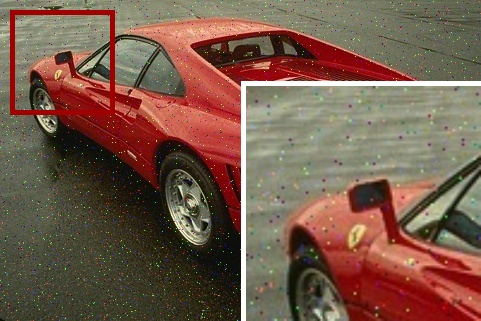
\includegraphics[width=\textwidth]{./figures/sensor/berkeley/29030_noisy_frame.jpg}\vspace{0.1cm}\\
    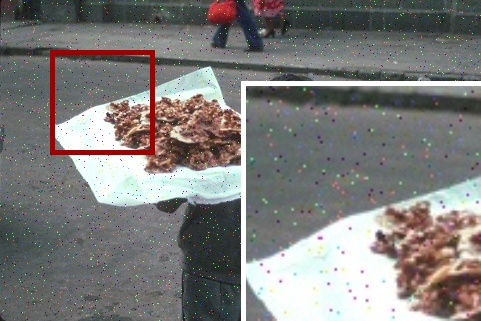
\includegraphics[width=\textwidth]{./figures/sensor/berkeley/90076_noisy_frame.jpg}\vspace{0.1cm}\\
    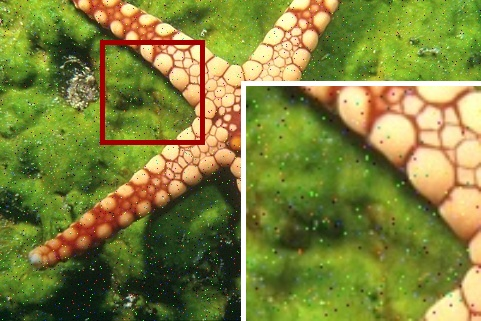
\includegraphics[width=\textwidth]{./figures/sensor/berkeley/12003_noisy_frame.jpg}\vspace{0.1cm}\\
    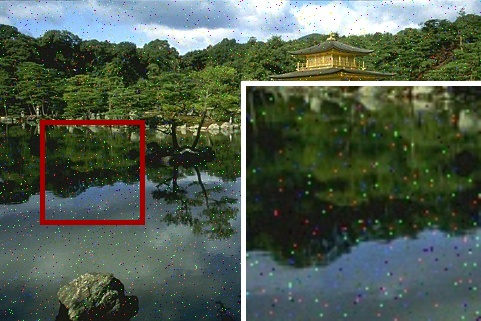
\includegraphics[width=\textwidth]{./figures/sensor/berkeley/65010_noisy_frame.jpg}\vspace{0.1cm}\\
    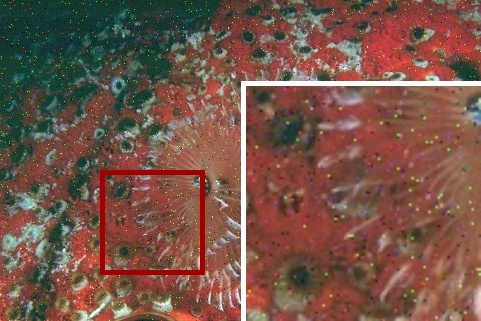
\includegraphics[width=\textwidth]{./figures/sensor/berkeley/12084_noisy_frame.jpg}\vspace{0.1cm}\\
    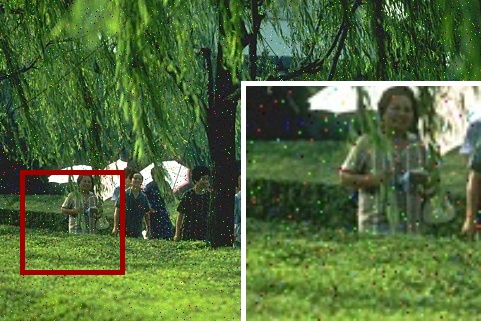
\includegraphics[width=\textwidth]{./figures/sensor/berkeley/65033_noisy_frame.jpg}\vspace{0.1cm}\\
    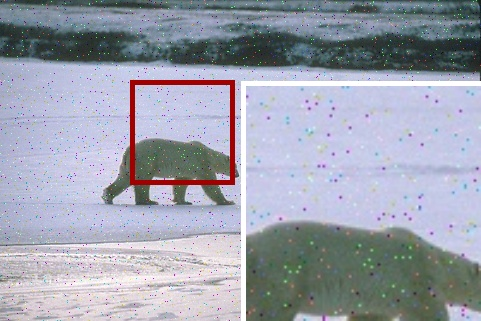
\includegraphics[width=\textwidth]{./figures/sensor/berkeley/100007_noisy_frame.jpg}%
    \caption{Noisy image.}
  \end{subfigure}\hfill
  \begin{subfigure}[]{0.22\textwidth}
    \centering
    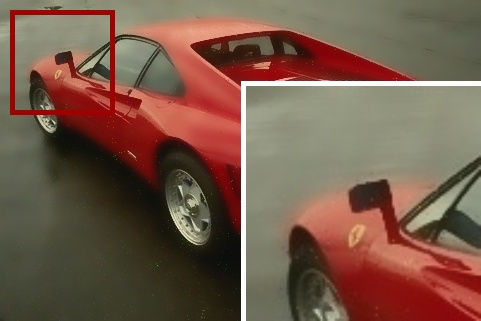
\includegraphics[width=\textwidth]{./figures/sensor/berkeley/29030_bilateral_frame.jpg}\vspace{0.1cm}\\
    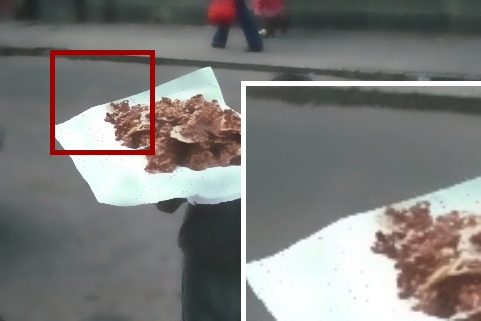
\includegraphics[width=\textwidth]{./figures/sensor/berkeley/90076_bilateral_frame.jpg}\vspace{0.1cm}\\
    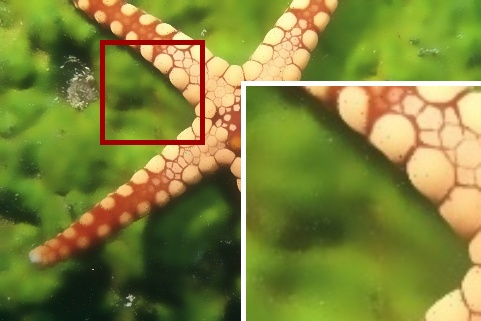
\includegraphics[width=\textwidth]{./figures/sensor/berkeley/12003_bilateral_frame.jpg}\vspace{0.1cm}\\
    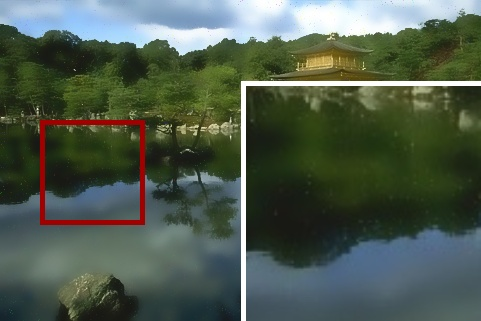
\includegraphics[width=\textwidth]{./figures/sensor/berkeley/65010_bilateral_frame.jpg}\vspace{0.1cm}\\
    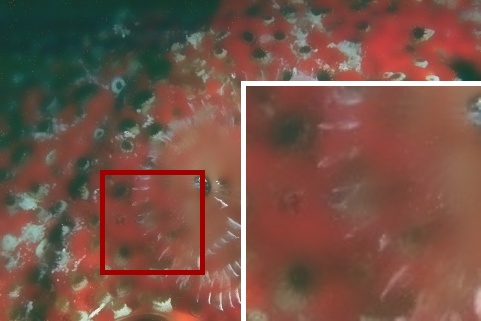
\includegraphics[width=\textwidth]{./figures/sensor/berkeley/12084_bilateral_frame.jpg}\vspace{0.1cm}\\
    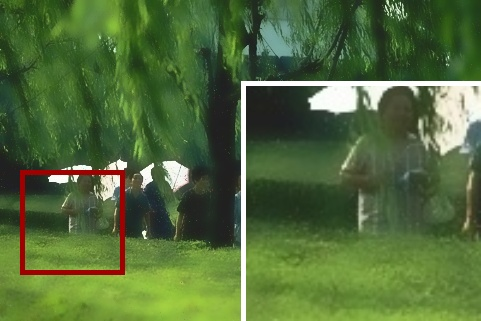
\includegraphics[width=\textwidth]{./figures/sensor/berkeley/65033_bilateral_frame.jpg}\vspace{0.1cm}\\
    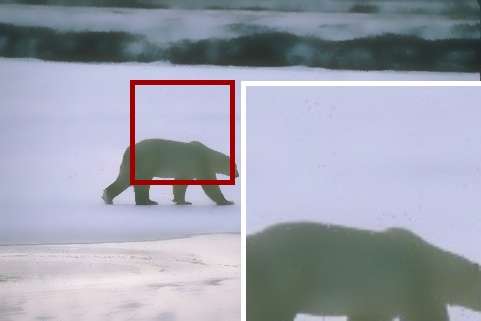
\includegraphics[width=\textwidth]{./figures/sensor/berkeley/100007_bilateral_frame.jpg}%
    \caption{Bilateral Filter.}
  \end{subfigure}\hfill
  \begin{subfigure}[]{0.22\textwidth}
    \centering
    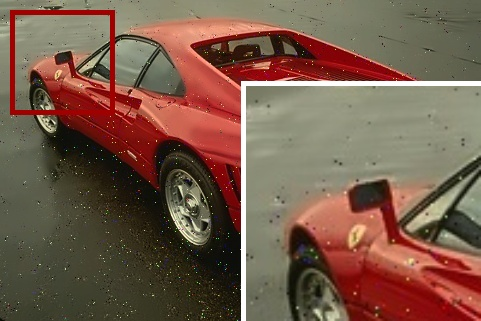
\includegraphics[width=\textwidth]{./figures/sensor/berkeley/29030_nonlocalmeans_frame.jpg}\vspace{0.1cm}\\
    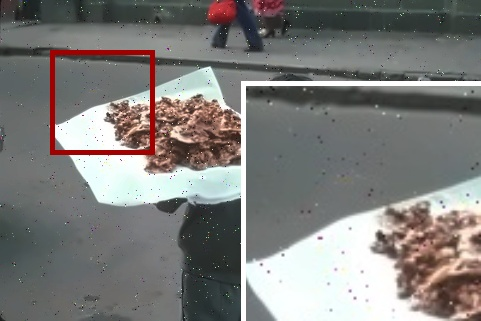
\includegraphics[width=\textwidth]{./figures/sensor/berkeley/90076_nonlocalmeans_frame.jpg}\vspace{0.1cm}\\
    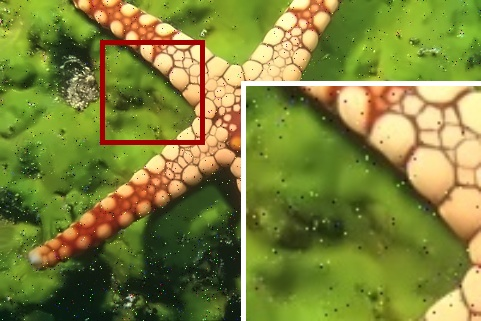
\includegraphics[width=\textwidth]{./figures/sensor/berkeley/12003_nonlocalmeans_frame.jpg}\vspace{0.1cm}\\
    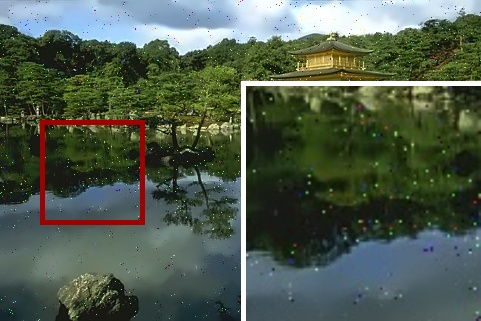
\includegraphics[width=\textwidth]{./figures/sensor/berkeley/65010_nonlocalmeans_frame.jpg}\vspace{0.1cm}\\
    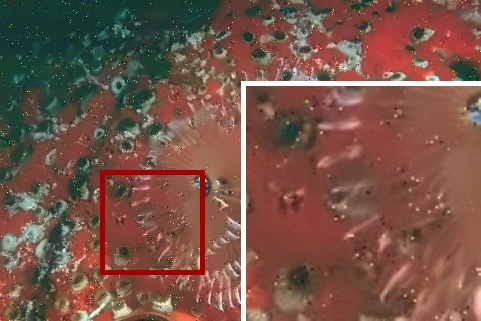
\includegraphics[width=\textwidth]{./figures/sensor/berkeley/12084_nonlocalmeans_frame.jpg}\vspace{0.1cm}\\
    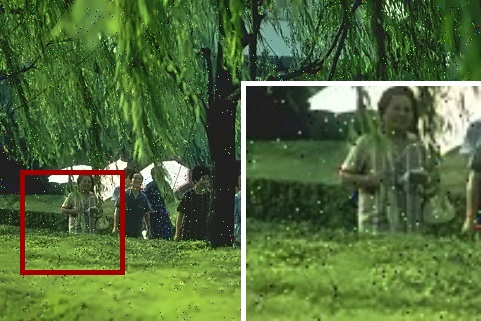
\includegraphics[width=\textwidth]{./figures/sensor/berkeley/65033_nonlocalmeans_frame.jpg}\vspace{0.1cm}\\
    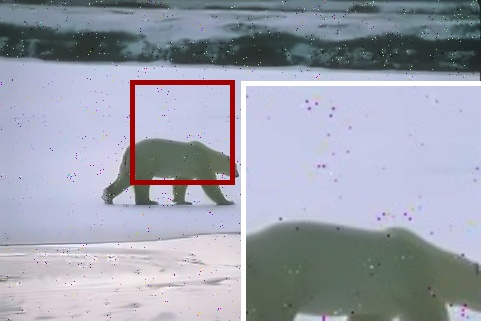
\includegraphics[width=\textwidth]{./figures/sensor/berkeley/100007_nonlocalmeans_frame.jpg}%
    \caption{NLM Filter.}
  \end{subfigure}\hfill
  \begin{subfigure}[]{0.22\textwidth}
    \centering
    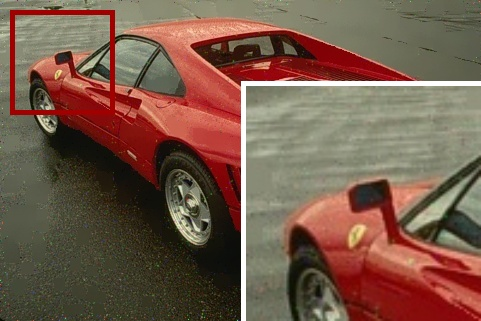
\includegraphics[width=\textwidth]{./figures/sensor/berkeley/29030_edgefilter_frame.jpg}\vspace{0.1cm}\\
    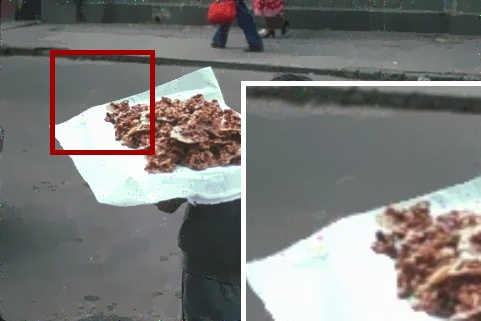
\includegraphics[width=\textwidth]{./figures/sensor/berkeley/90076_edgefilter_frame.jpg}\vspace{0.1cm}\\
    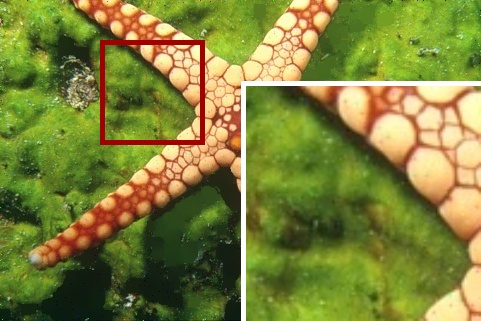
\includegraphics[width=\textwidth]{./figures/sensor/berkeley/12003_edgefilter_frame.jpg}\vspace{0.1cm}\\
    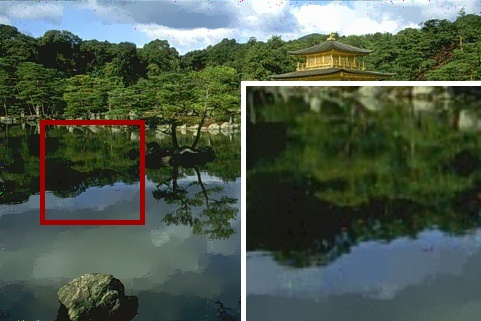
\includegraphics[width=\textwidth]{./figures/sensor/berkeley/65010_edgefilter_frame.jpg}\vspace{0.1cm}\\
    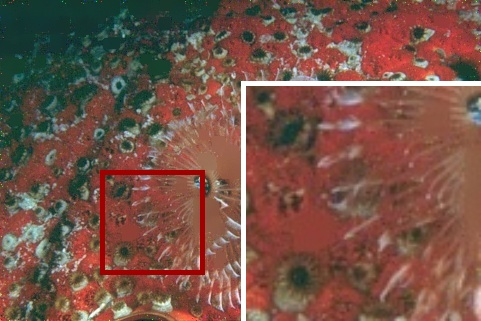
\includegraphics[width=\textwidth]{./figures/sensor/berkeley/12084_edgefilter_frame.jpg}\vspace{0.1cm}\\
    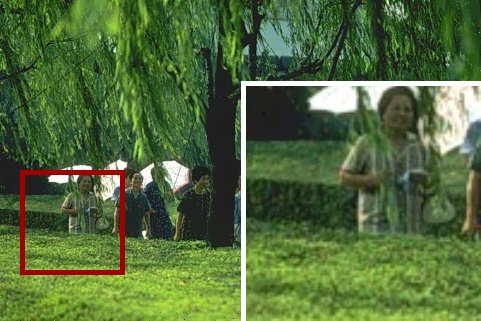
\includegraphics[width=\textwidth]{./figures/sensor/berkeley/65033_edgefilter_frame.jpg}\vspace{0.1cm}\\
    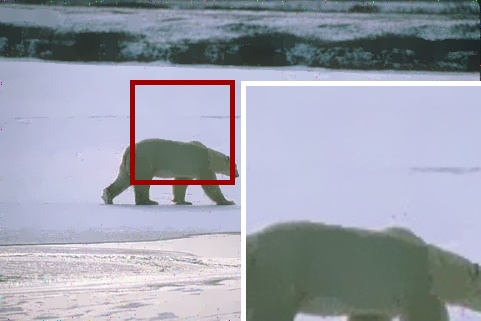
\includegraphics[width=\textwidth]{./figures/sensor/berkeley/100007_edgefilter_frame.jpg}%
    \caption{Proposed EPF.}
  \end{subfigure}%
  \caption{Visual comparison of filter results. Quantitative results are shown in \tabref{tab:experiments_rmsepsnr}. Images taken from Berkeley Image Data Set~\cite{arbelaez2011contour}.}
  \label{fig:sensor_experiments_examples}
\end{figure}

The proposed filter achieves on both data sets the best performance markers. 
In the discussion, see \secref{sec:perception_discussion}, the results are also compared to more recent, state-of-the-art algorithms.

\begin{table}[]
  \centering
  \begin{tabular}{lcccc}
    \toprule
      & \multicolumn{2}{c}{Berkeley Data Set}    & \multicolumn{2}{c}{Coco Data Set}\\
      & RMSE  & PSNR                       & RMSE  & PSNR\\
    \midrule
    Original        & $17.95$ & $23.31$ & $17.31$ & $23.33$\\
    EPF             & \bm{$7.06$} & \bm{$31.05$} & \bm{$7.89$} & \bm{$30.47$}\\
    Bilateral       & $10.41$ & $27.75$ & $10.43$ & $28.01$\\
    Gaussian        & $14.59$ & $25.08$ & $15.69$ & $24.81$\\
    Median          & $14.04$ & $25.63$ & $14.91$ & $25.54$\\
    NLM             & $11.40$ & $26.86$ & $12.28$ & $26.44$\\
    \bottomrule
  \end{tabular}
  \caption{\gls{ac:rmse} and \gls{ac:psnr} computed on the Berkeley Data Set (500 images) and the Coco Data Set (40775 images). The first line ``Original'' refers to the not denoised image. The error is $\pm 0.01$ for all values.}
  \label{tab:experiments_rmsepsnr}
\end{table}





\subsection{Denoising of 1d sensor data}

As already suggested in \figref{fig:sensor_method_example}, \figref{fig:sensor_experiments_subwindowsize}, and \figref{fig:sensor_experiments_threshold}, the filter can also be applied to 1d data. 
This may happen, for example, as a post-processing step for sensor readings. 
The filter is tested on three different settings: first, an alternating line, which switches every 100 samples its height to either $f(x) = f_{min}$ or $f(x) = f_{max}$; second, a sawtooth wave defined by $f(x) = x - \operatorname{floor}_{100}(x)$; and third, a sinusoidal wave $f(x) = \sin{2 \pi x / 250}$ with a wave length of 250 data points.
Every data line consists of a total length of 1000 samples.
To each scenario either Gaussian noise with variance of $\sigma = 10$, salt-and-pepper noise (to 5\% of samples), or both is added. 
Visual examples are shown in \figref{fig:sensor_experiments_1d_altline}, \figref{fig:sensor_experiments_1d_sawtooth}, and \figref{fig:sensor_experiments_1d_sinus}.

Again, the proposed filter ($N = 11$, $\tau = 30$) is compared to a Gaussian blurring filter (kernel: \unit[$7 \times 7$]{px}, $\sigma_{x,y} = 3$), a bilateral filter ($\sigma_c = 30$, $\sigma_s = 30$, and a median filter (kernel size: \unit[$9$]{px}). 
\gls{ac:rmse} and \gls{ac:psnr} is computed according to \eqnref{eq:rmse} and \eqnref{eq:psnr}.
On each setting 1000 trials are performed and averaged.
Results are shown in \tabref{tab:experiments_1d_rmsepsnr}.

In almost all experiments \gls{ac:epf} outperforms other standard 1d filtering methods.
While the median filter performs very well on salt-and-pepper noise, it is not edge preserving and thus introduces artefacts on edges.
The bilateral filter on the other hand, handles edges very well, but has significant trouble with removing salt-and-pepper noise.
The proposed \gls{ac:epf} filter performs well on both, Gaussian and salt-and-pepper noise and is edge preserving.

  \begin{table}[]
  \centering
  \begin{tabular}{c l cc|cc|cc}
    \toprule
    && \multicolumn{2}{c}{Gauss}    & \multicolumn{2}{c}{s\&p}& \multicolumn{2}{c}{Gauss and s\&p}                \\
    &             & RMSE         & PSNR          & RMSE          & PSNR          & RMSE          & PSNR           \\
    \midrule
    \multirow{5}{*}{\rotatebox[origin=c]{90}{\makecell{1) Alternating\\Line \vspace{0.25cm}\\ 
\includegraphics[width=1.5cm]{./figures/sensor/experiments_alternatingline.png}}}} & No denoising & $10.0$       & $22.3$        & $15.2$        & $16.4$         & $18.1$        & $17.2$        \\
    &EPF          & \bm{$2.6$}   & \bm{$32.3}$   & \bm{$3.9$}    & \bm{$28.5$}    & \bm{$5.1$}    & \bm{$26.7$}   \\
    &Bilateral    & $6.9$        & $25.3$        & $15.2$        & $16.4$         & $16.5$        & $17.7$        \\
    &Gaussian     & $6.0$        & $25.3$        &  $7.8$        & $22.2$         &  $8.7$        & $22.1$        \\
    &Median       & $5.1$        & $26.8$        &  $4.1$        & $27.9$         &  $6.0$        & $25.4$        \\
    \midrule
    \multirow{5}{*}{\rotatebox[origin=c]{90}{\makecell{2) Sawtooth\\Wave \vspace{0.25cm}\\ 
\includegraphics[width=1.5cm]{./figures/sensor/experiments_sawtooth.png}}}} & No denoising &  $10.0$       & $21.6$        & $14.1$        & $17.1$        & $17.1$        & $17.0$        \\
    &EPF          &  \bm{$3.7$}   & \bm{$29.3$}   & \bm{$4.6$}    & \bm{$26.5$}   & \bm{$6.6$}    & \bm{$24.5$}   \\
    &Bilateral    &  $7.0$        & $24.4$        & $14.0$        & $17.1$        & $15.5$        & $17.5$        \\
    &Gaussian     &  $7.6$        & $22.6$        &  $8.8$        & $20.9$        &  $9.6$        & $20.6$        \\
    &Median       &  $5.7$        & $25.2$        &  $5.8$        & $24.9$        &  $7.4$        & $23.1$        \\
    \midrule
    \multirow{5}{*}{\rotatebox[origin=c]{90}{\makecell{3) Sinusoidal\\Wave \vspace{0.25cm}\\ 
\includegraphics[width=1.5cm]{./figures/sensor/experiments_sinusoidal.png}}}} & No denoising & $10.0$        & $20.1$        & $12.9$        & $17.8$        & $16.1$        & $16.0$        \\
    &EPF          & \bm{$2.7$}    & \bm{$29.5$}   &  $2.6$        & $29.8$        & \bm{$4.4$}    & \bm{$25.6$}   \\
    &Bilateral    & $6.7$         & $23.0$        & $12.8$        & $17.9$        & $14.4$        & $16.9$        \\
    &Gaussian     & $3.9$         & $26.7$        &  $5.0$        & $24.2$        &  $6.3$        & $22.6$        \\
    &Median       & $4.1$         & $26.1$        & \bm{$0.6$}    & \bm{$46.1$}   &  $4.5$        & $25.6$        \\
    \bottomrule
  \end{tabular}
  \caption{Comparison of \gls{ac:rmse} and \gls{ac:psnr} computed on three different scenarios: 1) an alternating line, 2) a sawtooth wave, and 3) a sinusoidal wave. To each scene three different noise types (Gaussian, salt-and-pepper (s\&p), or both) are added, resulting in 9 different experiments. Each experiment is repeated 1000 times and averaged; the error is $\pm 0.1$ for all values.}
  \label{tab:experiments_1d_rmsepsnr}
\end{table}

\begin{figure}[]
  \centering
  \begin{subfigure}[]{\textwidth}
    \centering
    \begin{tikzpicture}[gnuplot]
%% generated with GNUPLOT 5.2p2 (Gentoo revision r0) (Lua 5.1; terminal rev. 99, script rev. 102)
%% Thu 28 Jun 2018 01:37:10 PM CEST
\gpcolor{color=gp lt color axes}
\gpsetlinetype{gp lt axes}
\gpsetdashtype{gp dt axes}
\gpsetlinewidth{0.50}
\draw[gp path] (1.564,1.898)--(13.564,1.898);
\gpcolor{color=gp lt color border}
\gpsetlinetype{gp lt border}
\gpsetdashtype{gp dt solid}
\gpsetlinewidth{1.00}
\draw[gp path] (1.564,1.898)--(1.777,1.898);
\node[gp node right] at (1.346,1.898) {$0$};
\gpcolor{color=gp lt color axes}
\gpsetlinetype{gp lt axes}
\gpsetdashtype{gp dt axes}
\gpsetlinewidth{0.50}
\draw[gp path] (1.564,2.399)--(13.564,2.399);
\gpcolor{color=gp lt color border}
\gpsetlinetype{gp lt border}
\gpsetdashtype{gp dt solid}
\gpsetlinewidth{1.00}
\draw[gp path] (1.564,2.399)--(1.777,2.399);
\node[gp node right] at (1.346,2.399) {$20$};
\gpcolor{color=gp lt color axes}
\gpsetlinetype{gp lt axes}
\gpsetdashtype{gp dt axes}
\gpsetlinewidth{0.50}
\draw[gp path] (1.564,2.898)--(13.564,2.898);
\gpcolor{color=gp lt color border}
\gpsetlinetype{gp lt border}
\gpsetdashtype{gp dt solid}
\gpsetlinewidth{1.00}
\draw[gp path] (1.564,2.898)--(1.777,2.898);
\node[gp node right] at (1.346,2.898) {$40$};
\gpcolor{color=gp lt color axes}
\gpsetlinetype{gp lt axes}
\gpsetdashtype{gp dt axes}
\gpsetlinewidth{0.50}
\draw[gp path] (1.564,3.399)--(13.564,3.399);
\gpcolor{color=gp lt color border}
\gpsetlinetype{gp lt border}
\gpsetdashtype{gp dt solid}
\gpsetlinewidth{1.00}
\draw[gp path] (1.564,3.399)--(1.777,3.399);
\node[gp node right] at (1.346,3.399) {$60$};
\gpcolor{color=gp lt color axes}
\gpsetlinetype{gp lt axes}
\gpsetdashtype{gp dt axes}
\gpsetlinewidth{0.50}
\draw[gp path] (1.564,3.900)--(13.564,3.900);
\gpcolor{color=gp lt color border}
\gpsetlinetype{gp lt border}
\gpsetdashtype{gp dt solid}
\gpsetlinewidth{1.00}
\draw[gp path] (1.564,3.900)--(1.777,3.900);
\node[gp node right] at (1.346,3.900) {$80$};
\gpcolor{color=gp lt color axes}
\gpsetlinetype{gp lt axes}
\gpsetdashtype{gp dt axes}
\gpsetlinewidth{0.50}
\draw[gp path] (1.564,4.399)--(13.564,4.399);
\gpcolor{color=gp lt color border}
\gpsetlinetype{gp lt border}
\gpsetdashtype{gp dt solid}
\gpsetlinewidth{1.00}
\draw[gp path] (1.564,4.399)--(1.777,4.399);
\node[gp node right] at (1.346,4.399) {$100$};
\gpcolor{color=gp lt color axes}
\gpsetlinetype{gp lt axes}
\gpsetdashtype{gp dt axes}
\gpsetlinewidth{0.50}
\draw[gp path] (1.564,4.900)--(13.564,4.900);
\gpcolor{color=gp lt color border}
\gpsetlinetype{gp lt border}
\gpsetdashtype{gp dt solid}
\gpsetlinewidth{1.00}
\draw[gp path] (1.564,4.900)--(1.777,4.900);
\node[gp node right] at (1.346,4.900) {$120$};
\draw[gp path] (1.564,1.649)--(1.564,2.020);
\node[gp node center] at (1.564,1.014) {$0$};
\draw[gp path] (3.964,1.649)--(3.964,2.020);
\node[gp node center] at (3.964,1.014) {$50$};
\draw[gp path] (6.364,1.649)--(6.364,2.020);
\node[gp node center] at (6.364,1.014) {$100$};
\draw[gp path] (8.764,1.649)--(8.764,2.020);
\node[gp node center] at (8.764,1.014) {$150$};
\draw[gp path] (11.165,1.649)--(11.165,2.020);
\node[gp node center] at (11.165,1.014) {$200$};
\draw[gp path] (13.564,1.649)--(13.564,2.020);
\node[gp node center] at (13.564,1.014) {$250$};
\draw[gp path] (1.564,5.149)--(1.564,1.649)--(13.564,1.649)--(13.564,5.149)--cycle;
\node[gp node center,rotate=-270] at (0.109,3.399) {Artificial sensor [a.u.]};
\node[gp node center] at (7.564,0.441) {Time [a.u.]};
\node[gp node right] at (6.042,6.604) {Noisy data};
\gpcolor{rgb color={0.667,0.000,0.000}}
\gpsetlinewidth{3.00}
\gpsetpointsize{4.00}
\gppoint{gp mark 2}{(1.564,2.649)}
\gppoint{gp mark 2}{(1.613,2.649)}
\gppoint{gp mark 2}{(1.660,2.649)}
\gppoint{gp mark 2}{(1.709,2.649)}
\gppoint{gp mark 2}{(1.756,2.649)}
\gppoint{gp mark 2}{(1.805,2.649)}
\gppoint{gp mark 2}{(1.852,2.649)}
\gppoint{gp mark 2}{(1.901,2.649)}
\gppoint{gp mark 2}{(1.948,2.649)}
\gppoint{gp mark 2}{(1.997,2.649)}
\gppoint{gp mark 2}{(2.044,2.649)}
\gppoint{gp mark 2}{(2.093,2.649)}
\gppoint{gp mark 2}{(2.140,4.399)}
\gppoint{gp mark 2}{(2.189,2.649)}
\gppoint{gp mark 2}{(2.236,2.649)}
\gppoint{gp mark 2}{(2.285,2.649)}
\gppoint{gp mark 2}{(2.332,2.649)}
\gppoint{gp mark 2}{(2.381,2.649)}
\gppoint{gp mark 2}{(2.428,2.649)}
\gppoint{gp mark 2}{(2.477,2.649)}
\gppoint{gp mark 2}{(2.524,2.649)}
\gppoint{gp mark 2}{(2.573,2.649)}
\gppoint{gp mark 2}{(2.620,2.649)}
\gppoint{gp mark 2}{(2.669,2.649)}
\gppoint{gp mark 2}{(2.716,2.649)}
\gppoint{gp mark 2}{(2.764,2.649)}
\gppoint{gp mark 2}{(2.812,2.649)}
\gppoint{gp mark 2}{(2.860,2.649)}
\gppoint{gp mark 2}{(2.908,2.649)}
\gppoint{gp mark 2}{(2.956,2.649)}
\gppoint{gp mark 2}{(3.004,2.649)}
\gppoint{gp mark 2}{(3.052,2.649)}
\gppoint{gp mark 2}{(3.100,2.649)}
\gppoint{gp mark 2}{(3.148,2.649)}
\gppoint{gp mark 2}{(3.196,2.649)}
\gppoint{gp mark 2}{(3.244,2.649)}
\gppoint{gp mark 2}{(3.292,1.898)}
\gppoint{gp mark 2}{(3.340,2.649)}
\gppoint{gp mark 2}{(3.388,2.649)}
\gppoint{gp mark 2}{(3.436,2.649)}
\gppoint{gp mark 2}{(3.484,2.649)}
\gppoint{gp mark 2}{(3.532,2.649)}
\gppoint{gp mark 2}{(3.580,2.649)}
\gppoint{gp mark 2}{(3.628,2.649)}
\gppoint{gp mark 2}{(3.676,2.649)}
\gppoint{gp mark 2}{(3.724,2.649)}
\gppoint{gp mark 2}{(3.772,2.649)}
\gppoint{gp mark 2}{(3.820,2.649)}
\gppoint{gp mark 2}{(3.868,2.649)}
\gppoint{gp mark 2}{(3.916,2.649)}
\gppoint{gp mark 2}{(3.964,1.898)}
\gppoint{gp mark 2}{(4.012,2.649)}
\gppoint{gp mark 2}{(4.060,2.649)}
\gppoint{gp mark 2}{(4.108,2.649)}
\gppoint{gp mark 2}{(4.156,2.649)}
\gppoint{gp mark 2}{(4.204,2.649)}
\gppoint{gp mark 2}{(4.252,1.898)}
\gppoint{gp mark 2}{(4.300,2.649)}
\gppoint{gp mark 2}{(4.348,2.649)}
\gppoint{gp mark 2}{(4.396,2.649)}
\gppoint{gp mark 2}{(4.444,2.649)}
\gppoint{gp mark 2}{(4.492,2.649)}
\gppoint{gp mark 2}{(4.540,2.649)}
\gppoint{gp mark 2}{(4.588,1.898)}
\gppoint{gp mark 2}{(4.637,2.649)}
\gppoint{gp mark 2}{(4.684,2.649)}
\gppoint{gp mark 2}{(4.733,2.649)}
\gppoint{gp mark 2}{(4.780,2.649)}
\gppoint{gp mark 2}{(4.829,2.649)}
\gppoint{gp mark 2}{(4.876,1.898)}
\gppoint{gp mark 2}{(4.925,2.649)}
\gppoint{gp mark 2}{(4.972,2.649)}
\gppoint{gp mark 2}{(5.021,2.649)}
\gppoint{gp mark 2}{(5.068,2.649)}
\gppoint{gp mark 2}{(5.117,2.649)}
\gppoint{gp mark 2}{(5.164,2.649)}
\gppoint{gp mark 2}{(5.213,2.649)}
\gppoint{gp mark 2}{(5.260,2.649)}
\gppoint{gp mark 2}{(5.309,2.649)}
\gppoint{gp mark 2}{(5.356,4.399)}
\gppoint{gp mark 2}{(5.405,2.649)}
\gppoint{gp mark 2}{(5.452,2.649)}
\gppoint{gp mark 2}{(5.501,2.649)}
\gppoint{gp mark 2}{(5.548,2.649)}
\gppoint{gp mark 2}{(5.597,2.649)}
\gppoint{gp mark 2}{(5.644,2.649)}
\gppoint{gp mark 2}{(5.693,2.649)}
\gppoint{gp mark 2}{(5.740,2.649)}
\gppoint{gp mark 2}{(5.788,2.649)}
\gppoint{gp mark 2}{(5.836,2.649)}
\gppoint{gp mark 2}{(5.884,2.649)}
\gppoint{gp mark 2}{(5.932,2.649)}
\gppoint{gp mark 2}{(5.980,2.649)}
\gppoint{gp mark 2}{(6.028,2.649)}
\gppoint{gp mark 2}{(6.076,2.649)}
\gppoint{gp mark 2}{(6.124,2.649)}
\gppoint{gp mark 2}{(6.172,2.649)}
\gppoint{gp mark 2}{(6.220,2.649)}
\gppoint{gp mark 2}{(6.268,2.649)}
\gppoint{gp mark 2}{(6.316,2.649)}
\gppoint{gp mark 2}{(6.364,4.399)}
\gppoint{gp mark 2}{(6.412,4.399)}
\gppoint{gp mark 2}{(6.460,4.399)}
\gppoint{gp mark 2}{(6.508,4.399)}
\gppoint{gp mark 2}{(6.556,4.399)}
\gppoint{gp mark 2}{(6.604,4.399)}
\gppoint{gp mark 2}{(6.652,4.399)}
\gppoint{gp mark 2}{(6.700,4.399)}
\gppoint{gp mark 2}{(6.748,4.399)}
\gppoint{gp mark 2}{(6.796,4.399)}
\gppoint{gp mark 2}{(6.844,4.399)}
\gppoint{gp mark 2}{(6.892,4.399)}
\gppoint{gp mark 2}{(6.940,4.399)}
\gppoint{gp mark 2}{(6.988,4.399)}
\gppoint{gp mark 2}{(7.036,4.399)}
\gppoint{gp mark 2}{(7.084,4.399)}
\gppoint{gp mark 2}{(7.132,4.399)}
\gppoint{gp mark 2}{(7.180,4.399)}
\gppoint{gp mark 2}{(7.228,4.399)}
\gppoint{gp mark 2}{(7.276,4.399)}
\gppoint{gp mark 2}{(7.324,4.399)}
\gppoint{gp mark 2}{(7.372,4.399)}
\gppoint{gp mark 2}{(7.420,4.399)}
\gppoint{gp mark 2}{(7.468,4.399)}
\gppoint{gp mark 2}{(7.516,4.399)}
\gppoint{gp mark 2}{(7.565,4.399)}
\gppoint{gp mark 2}{(7.612,4.399)}
\gppoint{gp mark 2}{(7.661,4.399)}
\gppoint{gp mark 2}{(7.708,4.399)}
\gppoint{gp mark 2}{(7.757,4.399)}
\gppoint{gp mark 2}{(7.804,4.399)}
\gppoint{gp mark 2}{(7.853,4.399)}
\gppoint{gp mark 2}{(7.900,4.399)}
\gppoint{gp mark 2}{(7.949,4.399)}
\gppoint{gp mark 2}{(7.996,4.399)}
\gppoint{gp mark 2}{(8.045,4.399)}
\gppoint{gp mark 2}{(8.092,4.399)}
\gppoint{gp mark 2}{(8.141,4.399)}
\gppoint{gp mark 2}{(8.188,4.399)}
\gppoint{gp mark 2}{(8.237,4.399)}
\gppoint{gp mark 2}{(8.284,4.399)}
\gppoint{gp mark 2}{(8.333,4.399)}
\gppoint{gp mark 2}{(8.380,4.399)}
\gppoint{gp mark 2}{(8.429,4.399)}
\gppoint{gp mark 2}{(8.476,4.399)}
\gppoint{gp mark 2}{(8.525,4.399)}
\gppoint{gp mark 2}{(8.572,4.399)}
\gppoint{gp mark 2}{(8.621,4.399)}
\gppoint{gp mark 2}{(8.668,4.399)}
\gppoint{gp mark 2}{(8.717,4.399)}
\gppoint{gp mark 2}{(8.764,4.399)}
\gppoint{gp mark 2}{(8.812,4.399)}
\gppoint{gp mark 2}{(8.860,4.399)}
\gppoint{gp mark 2}{(8.908,4.399)}
\gppoint{gp mark 2}{(8.956,4.399)}
\gppoint{gp mark 2}{(9.004,4.399)}
\gppoint{gp mark 2}{(9.052,4.399)}
\gppoint{gp mark 2}{(9.100,4.399)}
\gppoint{gp mark 2}{(9.148,4.399)}
\gppoint{gp mark 2}{(9.196,4.399)}
\gppoint{gp mark 2}{(9.244,4.399)}
\gppoint{gp mark 2}{(9.292,4.399)}
\gppoint{gp mark 2}{(9.340,4.399)}
\gppoint{gp mark 2}{(9.388,4.399)}
\gppoint{gp mark 2}{(9.436,4.399)}
\gppoint{gp mark 2}{(9.484,4.399)}
\gppoint{gp mark 2}{(9.532,4.399)}
\gppoint{gp mark 2}{(9.580,4.399)}
\gppoint{gp mark 2}{(9.628,4.399)}
\gppoint{gp mark 2}{(9.676,4.399)}
\gppoint{gp mark 2}{(9.724,1.898)}
\gppoint{gp mark 2}{(9.772,4.399)}
\gppoint{gp mark 2}{(9.820,4.399)}
\gppoint{gp mark 2}{(9.868,4.399)}
\gppoint{gp mark 2}{(9.916,4.399)}
\gppoint{gp mark 2}{(9.964,4.399)}
\gppoint{gp mark 2}{(10.012,4.399)}
\gppoint{gp mark 2}{(10.060,4.399)}
\gppoint{gp mark 2}{(10.108,4.399)}
\gppoint{gp mark 2}{(10.156,4.399)}
\gppoint{gp mark 2}{(10.204,4.399)}
\gppoint{gp mark 2}{(10.252,4.399)}
\gppoint{gp mark 2}{(10.300,4.399)}
\gppoint{gp mark 2}{(10.348,4.399)}
\gppoint{gp mark 2}{(10.396,4.399)}
\gppoint{gp mark 2}{(10.444,4.399)}
\gppoint{gp mark 2}{(10.492,4.399)}
\gppoint{gp mark 2}{(10.540,4.399)}
\gppoint{gp mark 2}{(10.589,4.399)}
\gppoint{gp mark 2}{(10.636,4.399)}
\gppoint{gp mark 2}{(10.685,4.399)}
\gppoint{gp mark 2}{(10.732,4.399)}
\gppoint{gp mark 2}{(10.781,4.399)}
\gppoint{gp mark 2}{(10.828,4.399)}
\gppoint{gp mark 2}{(10.877,4.399)}
\gppoint{gp mark 2}{(10.924,4.399)}
\gppoint{gp mark 2}{(10.973,4.399)}
\gppoint{gp mark 2}{(11.020,1.898)}
\gppoint{gp mark 2}{(11.069,4.399)}
\gppoint{gp mark 2}{(11.116,4.399)}
\gppoint{gp mark 2}{(11.165,4.399)}
\gppoint{gp mark 2}{(11.212,2.649)}
\gppoint{gp mark 2}{(11.261,4.399)}
\gppoint{gp mark 2}{(11.308,2.649)}
\gppoint{gp mark 2}{(11.357,2.649)}
\gppoint{gp mark 2}{(11.404,2.649)}
\gppoint{gp mark 2}{(11.453,2.649)}
\gppoint{gp mark 2}{(11.500,2.649)}
\gppoint{gp mark 2}{(11.549,2.649)}
\gppoint{gp mark 2}{(11.596,2.649)}
\gppoint{gp mark 2}{(11.645,2.649)}
\gppoint{gp mark 2}{(11.692,2.649)}
\gppoint{gp mark 2}{(11.740,4.399)}
\gppoint{gp mark 2}{(11.788,2.649)}
\gppoint{gp mark 2}{(11.836,2.649)}
\gppoint{gp mark 2}{(11.884,2.649)}
\gppoint{gp mark 2}{(11.932,2.649)}
\gppoint{gp mark 2}{(11.980,2.649)}
\gppoint{gp mark 2}{(12.028,2.649)}
\gppoint{gp mark 2}{(12.076,2.649)}
\gppoint{gp mark 2}{(12.124,2.649)}
\gppoint{gp mark 2}{(12.172,2.649)}
\gppoint{gp mark 2}{(12.220,2.649)}
\gppoint{gp mark 2}{(12.268,2.649)}
\gppoint{gp mark 2}{(12.316,4.399)}
\gppoint{gp mark 2}{(12.364,2.649)}
\gppoint{gp mark 2}{(12.412,2.649)}
\gppoint{gp mark 2}{(12.460,2.649)}
\gppoint{gp mark 2}{(12.508,2.649)}
\gppoint{gp mark 2}{(12.556,2.649)}
\gppoint{gp mark 2}{(12.604,1.898)}
\gppoint{gp mark 2}{(12.652,2.649)}
\gppoint{gp mark 2}{(12.700,2.649)}
\gppoint{gp mark 2}{(12.748,2.649)}
\gppoint{gp mark 2}{(12.796,2.649)}
\gppoint{gp mark 2}{(12.844,2.649)}
\gppoint{gp mark 2}{(12.892,2.649)}
\gppoint{gp mark 2}{(12.940,2.649)}
\gppoint{gp mark 2}{(12.988,4.399)}
\gppoint{gp mark 2}{(13.036,2.649)}
\gppoint{gp mark 2}{(13.084,2.649)}
\gppoint{gp mark 2}{(13.132,2.649)}
\gppoint{gp mark 2}{(13.180,2.649)}
\gppoint{gp mark 2}{(13.228,2.649)}
\gppoint{gp mark 2}{(13.276,2.649)}
\gppoint{gp mark 2}{(13.324,4.399)}
\gppoint{gp mark 2}{(13.372,2.649)}
\gppoint{gp mark 2}{(13.420,2.649)}
\gppoint{gp mark 2}{(13.468,2.649)}
\gppoint{gp mark 2}{(13.516,2.649)}
\gppoint{gp mark 2}{(13.564,2.649)}
\gppoint{gp mark 2}{(6.803,6.604)}
\gpcolor{color=gp lt color border}
\node[gp node right] at (6.042,6.128) {Bilateral Filter};
\gpcolor{rgb color={0.000,0.000,0.667}}
\gppoint{gp mark 3}{(1.564,2.649)}
\gppoint{gp mark 3}{(1.613,2.649)}
\gppoint{gp mark 3}{(1.660,2.649)}
\gppoint{gp mark 3}{(1.709,2.649)}
\gppoint{gp mark 3}{(1.756,2.649)}
\gppoint{gp mark 3}{(1.805,2.649)}
\gppoint{gp mark 3}{(1.852,2.649)}
\gppoint{gp mark 3}{(1.901,2.649)}
\gppoint{gp mark 3}{(1.948,2.649)}
\gppoint{gp mark 3}{(1.997,2.649)}
\gppoint{gp mark 3}{(2.044,2.649)}
\gppoint{gp mark 3}{(2.093,2.649)}
\gppoint{gp mark 3}{(2.140,4.399)}
\gppoint{gp mark 3}{(2.189,2.649)}
\gppoint{gp mark 3}{(2.236,2.649)}
\gppoint{gp mark 3}{(2.285,2.649)}
\gppoint{gp mark 3}{(2.332,2.649)}
\gppoint{gp mark 3}{(2.381,2.649)}
\gppoint{gp mark 3}{(2.428,2.649)}
\gppoint{gp mark 3}{(2.477,2.649)}
\gppoint{gp mark 3}{(2.524,2.649)}
\gppoint{gp mark 3}{(2.573,2.649)}
\gppoint{gp mark 3}{(2.620,2.649)}
\gppoint{gp mark 3}{(2.669,2.649)}
\gppoint{gp mark 3}{(2.716,2.649)}
\gppoint{gp mark 3}{(2.764,2.649)}
\gppoint{gp mark 3}{(2.812,2.649)}
\gppoint{gp mark 3}{(2.860,2.649)}
\gppoint{gp mark 3}{(2.908,2.649)}
\gppoint{gp mark 3}{(2.956,2.649)}
\gppoint{gp mark 3}{(3.004,2.649)}
\gppoint{gp mark 3}{(3.052,2.649)}
\gppoint{gp mark 3}{(3.100,2.649)}
\gppoint{gp mark 3}{(3.148,2.649)}
\gppoint{gp mark 3}{(3.196,2.649)}
\gppoint{gp mark 3}{(3.244,2.649)}
\gppoint{gp mark 3}{(3.292,1.948)}
\gppoint{gp mark 3}{(3.340,2.649)}
\gppoint{gp mark 3}{(3.388,2.649)}
\gppoint{gp mark 3}{(3.436,2.649)}
\gppoint{gp mark 3}{(3.484,2.649)}
\gppoint{gp mark 3}{(3.532,2.649)}
\gppoint{gp mark 3}{(3.580,2.649)}
\gppoint{gp mark 3}{(3.628,2.649)}
\gppoint{gp mark 3}{(3.676,2.649)}
\gppoint{gp mark 3}{(3.724,2.649)}
\gppoint{gp mark 3}{(3.772,2.649)}
\gppoint{gp mark 3}{(3.820,2.649)}
\gppoint{gp mark 3}{(3.868,2.649)}
\gppoint{gp mark 3}{(3.916,2.649)}
\gppoint{gp mark 3}{(3.964,1.948)}
\gppoint{gp mark 3}{(4.012,2.649)}
\gppoint{gp mark 3}{(4.060,2.647)}
\gppoint{gp mark 3}{(4.108,2.647)}
\gppoint{gp mark 3}{(4.156,2.647)}
\gppoint{gp mark 3}{(4.204,2.649)}
\gppoint{gp mark 3}{(4.252,1.948)}
\gppoint{gp mark 3}{(4.300,2.649)}
\gppoint{gp mark 3}{(4.348,2.649)}
\gppoint{gp mark 3}{(4.396,2.647)}
\gppoint{gp mark 3}{(4.444,2.647)}
\gppoint{gp mark 3}{(4.492,2.649)}
\gppoint{gp mark 3}{(4.540,2.649)}
\gppoint{gp mark 3}{(4.588,1.948)}
\gppoint{gp mark 3}{(4.637,2.649)}
\gppoint{gp mark 3}{(4.684,2.647)}
\gppoint{gp mark 3}{(4.733,2.647)}
\gppoint{gp mark 3}{(4.780,2.647)}
\gppoint{gp mark 3}{(4.829,2.649)}
\gppoint{gp mark 3}{(4.876,1.948)}
\gppoint{gp mark 3}{(4.925,2.649)}
\gppoint{gp mark 3}{(4.972,2.649)}
\gppoint{gp mark 3}{(5.021,2.649)}
\gppoint{gp mark 3}{(5.068,2.649)}
\gppoint{gp mark 3}{(5.117,2.649)}
\gppoint{gp mark 3}{(5.164,2.649)}
\gppoint{gp mark 3}{(5.213,2.649)}
\gppoint{gp mark 3}{(5.260,2.649)}
\gppoint{gp mark 3}{(5.309,2.649)}
\gppoint{gp mark 3}{(5.356,4.399)}
\gppoint{gp mark 3}{(5.405,2.649)}
\gppoint{gp mark 3}{(5.452,2.649)}
\gppoint{gp mark 3}{(5.501,2.649)}
\gppoint{gp mark 3}{(5.548,2.649)}
\gppoint{gp mark 3}{(5.597,2.649)}
\gppoint{gp mark 3}{(5.644,2.649)}
\gppoint{gp mark 3}{(5.693,2.649)}
\gppoint{gp mark 3}{(5.740,2.649)}
\gppoint{gp mark 3}{(5.788,2.649)}
\gppoint{gp mark 3}{(5.836,2.649)}
\gppoint{gp mark 3}{(5.884,2.649)}
\gppoint{gp mark 3}{(5.932,2.649)}
\gppoint{gp mark 3}{(5.980,2.649)}
\gppoint{gp mark 3}{(6.028,2.649)}
\gppoint{gp mark 3}{(6.076,2.649)}
\gppoint{gp mark 3}{(6.124,2.649)}
\gppoint{gp mark 3}{(6.172,2.649)}
\gppoint{gp mark 3}{(6.220,2.649)}
\gppoint{gp mark 3}{(6.268,2.649)}
\gppoint{gp mark 3}{(6.316,2.649)}
\gppoint{gp mark 3}{(6.364,4.399)}
\gppoint{gp mark 3}{(6.412,4.399)}
\gppoint{gp mark 3}{(6.460,4.399)}
\gppoint{gp mark 3}{(6.508,4.399)}
\gppoint{gp mark 3}{(6.556,4.399)}
\gppoint{gp mark 3}{(6.604,4.399)}
\gppoint{gp mark 3}{(6.652,4.399)}
\gppoint{gp mark 3}{(6.700,4.399)}
\gppoint{gp mark 3}{(6.748,4.399)}
\gppoint{gp mark 3}{(6.796,4.399)}
\gppoint{gp mark 3}{(6.844,4.399)}
\gppoint{gp mark 3}{(6.892,4.399)}
\gppoint{gp mark 3}{(6.940,4.399)}
\gppoint{gp mark 3}{(6.988,4.399)}
\gppoint{gp mark 3}{(7.036,4.399)}
\gppoint{gp mark 3}{(7.084,4.399)}
\gppoint{gp mark 3}{(7.132,4.399)}
\gppoint{gp mark 3}{(7.180,4.399)}
\gppoint{gp mark 3}{(7.228,4.399)}
\gppoint{gp mark 3}{(7.276,4.399)}
\gppoint{gp mark 3}{(7.324,4.399)}
\gppoint{gp mark 3}{(7.372,4.399)}
\gppoint{gp mark 3}{(7.420,4.399)}
\gppoint{gp mark 3}{(7.468,4.399)}
\gppoint{gp mark 3}{(7.516,4.399)}
\gppoint{gp mark 3}{(7.565,4.399)}
\gppoint{gp mark 3}{(7.612,4.399)}
\gppoint{gp mark 3}{(7.661,4.399)}
\gppoint{gp mark 3}{(7.708,4.399)}
\gppoint{gp mark 3}{(7.757,4.399)}
\gppoint{gp mark 3}{(7.804,4.399)}
\gppoint{gp mark 3}{(7.853,4.399)}
\gppoint{gp mark 3}{(7.900,4.399)}
\gppoint{gp mark 3}{(7.949,4.399)}
\gppoint{gp mark 3}{(7.996,4.399)}
\gppoint{gp mark 3}{(8.045,4.399)}
\gppoint{gp mark 3}{(8.092,4.399)}
\gppoint{gp mark 3}{(8.141,4.399)}
\gppoint{gp mark 3}{(8.188,4.399)}
\gppoint{gp mark 3}{(8.237,4.399)}
\gppoint{gp mark 3}{(8.284,4.399)}
\gppoint{gp mark 3}{(8.333,4.399)}
\gppoint{gp mark 3}{(8.380,4.399)}
\gppoint{gp mark 3}{(8.429,4.399)}
\gppoint{gp mark 3}{(8.476,4.399)}
\gppoint{gp mark 3}{(8.525,4.399)}
\gppoint{gp mark 3}{(8.572,4.399)}
\gppoint{gp mark 3}{(8.621,4.399)}
\gppoint{gp mark 3}{(8.668,4.399)}
\gppoint{gp mark 3}{(8.717,4.399)}
\gppoint{gp mark 3}{(8.764,4.399)}
\gppoint{gp mark 3}{(8.812,4.399)}
\gppoint{gp mark 3}{(8.860,4.399)}
\gppoint{gp mark 3}{(8.908,4.399)}
\gppoint{gp mark 3}{(8.956,4.399)}
\gppoint{gp mark 3}{(9.004,4.399)}
\gppoint{gp mark 3}{(9.052,4.399)}
\gppoint{gp mark 3}{(9.100,4.399)}
\gppoint{gp mark 3}{(9.148,4.399)}
\gppoint{gp mark 3}{(9.196,4.399)}
\gppoint{gp mark 3}{(9.244,4.399)}
\gppoint{gp mark 3}{(9.292,4.399)}
\gppoint{gp mark 3}{(9.340,4.399)}
\gppoint{gp mark 3}{(9.388,4.399)}
\gppoint{gp mark 3}{(9.436,4.399)}
\gppoint{gp mark 3}{(9.484,4.399)}
\gppoint{gp mark 3}{(9.532,4.399)}
\gppoint{gp mark 3}{(9.580,4.399)}
\gppoint{gp mark 3}{(9.628,4.399)}
\gppoint{gp mark 3}{(9.676,4.399)}
\gppoint{gp mark 3}{(9.724,1.898)}
\gppoint{gp mark 3}{(9.772,4.399)}
\gppoint{gp mark 3}{(9.820,4.399)}
\gppoint{gp mark 3}{(9.868,4.399)}
\gppoint{gp mark 3}{(9.916,4.399)}
\gppoint{gp mark 3}{(9.964,4.399)}
\gppoint{gp mark 3}{(10.012,4.399)}
\gppoint{gp mark 3}{(10.060,4.399)}
\gppoint{gp mark 3}{(10.108,4.399)}
\gppoint{gp mark 3}{(10.156,4.399)}
\gppoint{gp mark 3}{(10.204,4.399)}
\gppoint{gp mark 3}{(10.252,4.399)}
\gppoint{gp mark 3}{(10.300,4.399)}
\gppoint{gp mark 3}{(10.348,4.399)}
\gppoint{gp mark 3}{(10.396,4.399)}
\gppoint{gp mark 3}{(10.444,4.399)}
\gppoint{gp mark 3}{(10.492,4.399)}
\gppoint{gp mark 3}{(10.540,4.399)}
\gppoint{gp mark 3}{(10.589,4.399)}
\gppoint{gp mark 3}{(10.636,4.399)}
\gppoint{gp mark 3}{(10.685,4.399)}
\gppoint{gp mark 3}{(10.732,4.399)}
\gppoint{gp mark 3}{(10.781,4.399)}
\gppoint{gp mark 3}{(10.828,4.399)}
\gppoint{gp mark 3}{(10.877,4.399)}
\gppoint{gp mark 3}{(10.924,4.399)}
\gppoint{gp mark 3}{(10.973,4.399)}
\gppoint{gp mark 3}{(11.020,1.905)}
\gppoint{gp mark 3}{(11.069,4.399)}
\gppoint{gp mark 3}{(11.116,4.399)}
\gppoint{gp mark 3}{(11.165,4.399)}
\gppoint{gp mark 3}{(11.212,2.647)}
\gppoint{gp mark 3}{(11.261,4.399)}
\gppoint{gp mark 3}{(11.308,2.649)}
\gppoint{gp mark 3}{(11.357,2.649)}
\gppoint{gp mark 3}{(11.404,2.649)}
\gppoint{gp mark 3}{(11.453,2.649)}
\gppoint{gp mark 3}{(11.500,2.649)}
\gppoint{gp mark 3}{(11.549,2.649)}
\gppoint{gp mark 3}{(11.596,2.649)}
\gppoint{gp mark 3}{(11.645,2.649)}
\gppoint{gp mark 3}{(11.692,2.649)}
\gppoint{gp mark 3}{(11.740,4.399)}
\gppoint{gp mark 3}{(11.788,2.649)}
\gppoint{gp mark 3}{(11.836,2.649)}
\gppoint{gp mark 3}{(11.884,2.649)}
\gppoint{gp mark 3}{(11.932,2.649)}
\gppoint{gp mark 3}{(11.980,2.649)}
\gppoint{gp mark 3}{(12.028,2.649)}
\gppoint{gp mark 3}{(12.076,2.649)}
\gppoint{gp mark 3}{(12.124,2.649)}
\gppoint{gp mark 3}{(12.172,2.649)}
\gppoint{gp mark 3}{(12.220,2.649)}
\gppoint{gp mark 3}{(12.268,2.649)}
\gppoint{gp mark 3}{(12.316,4.399)}
\gppoint{gp mark 3}{(12.364,2.649)}
\gppoint{gp mark 3}{(12.412,2.649)}
\gppoint{gp mark 3}{(12.460,2.649)}
\gppoint{gp mark 3}{(12.508,2.649)}
\gppoint{gp mark 3}{(12.556,2.649)}
\gppoint{gp mark 3}{(12.604,1.948)}
\gppoint{gp mark 3}{(12.652,2.649)}
\gppoint{gp mark 3}{(12.700,2.649)}
\gppoint{gp mark 3}{(12.748,2.649)}
\gppoint{gp mark 3}{(12.796,2.649)}
\gppoint{gp mark 3}{(12.844,2.649)}
\gppoint{gp mark 3}{(12.892,2.649)}
\gppoint{gp mark 3}{(12.940,2.649)}
\gppoint{gp mark 3}{(12.988,4.399)}
\gppoint{gp mark 3}{(13.036,2.649)}
\gppoint{gp mark 3}{(13.084,2.649)}
\gppoint{gp mark 3}{(13.132,2.649)}
\gppoint{gp mark 3}{(13.180,2.649)}
\gppoint{gp mark 3}{(13.228,2.649)}
\gppoint{gp mark 3}{(13.276,2.649)}
\gppoint{gp mark 3}{(13.324,4.399)}
\gppoint{gp mark 3}{(13.372,2.649)}
\gppoint{gp mark 3}{(13.420,2.649)}
\gppoint{gp mark 3}{(13.468,2.649)}
\gppoint{gp mark 3}{(13.516,2.649)}
\gppoint{gp mark 3}{(13.564,2.649)}
\gppoint{gp mark 3}{(6.803,6.128)}
\gpcolor{color=gp lt color border}
\node[gp node right] at (6.042,5.652) {Gaussian Filter};
\gpcolor{rgb color={0.902,0.624,0.000}}
\gpsetlinewidth{1.00}
\gppoint{gp mark 4}{(1.564,2.649)}
\gppoint{gp mark 4}{(1.613,2.649)}
\gppoint{gp mark 4}{(1.660,2.649)}
\gppoint{gp mark 4}{(1.709,2.649)}
\gppoint{gp mark 4}{(1.756,2.649)}
\gppoint{gp mark 4}{(1.805,2.649)}
\gppoint{gp mark 4}{(1.852,2.649)}
\gppoint{gp mark 4}{(1.901,2.649)}
\gppoint{gp mark 4}{(1.948,2.649)}
\gppoint{gp mark 4}{(1.997,2.834)}
\gppoint{gp mark 4}{(2.044,2.894)}
\gppoint{gp mark 4}{(2.093,2.939)}
\gppoint{gp mark 4}{(2.140,2.956)}
\gppoint{gp mark 4}{(2.189,2.939)}
\gppoint{gp mark 4}{(2.236,2.894)}
\gppoint{gp mark 4}{(2.285,2.834)}
\gppoint{gp mark 4}{(2.332,2.649)}
\gppoint{gp mark 4}{(2.381,2.649)}
\gppoint{gp mark 4}{(2.428,2.649)}
\gppoint{gp mark 4}{(2.477,2.649)}
\gppoint{gp mark 4}{(2.524,2.649)}
\gppoint{gp mark 4}{(2.573,2.649)}
\gppoint{gp mark 4}{(2.620,2.649)}
\gppoint{gp mark 4}{(2.669,2.649)}
\gppoint{gp mark 4}{(2.716,2.649)}
\gppoint{gp mark 4}{(2.764,2.649)}
\gppoint{gp mark 4}{(2.812,2.649)}
\gppoint{gp mark 4}{(2.860,2.649)}
\gppoint{gp mark 4}{(2.908,2.649)}
\gppoint{gp mark 4}{(2.956,2.649)}
\gppoint{gp mark 4}{(3.004,2.649)}
\gppoint{gp mark 4}{(3.052,2.649)}
\gppoint{gp mark 4}{(3.100,2.649)}
\gppoint{gp mark 4}{(3.148,2.568)}
\gppoint{gp mark 4}{(3.196,2.544)}
\gppoint{gp mark 4}{(3.244,2.525)}
\gppoint{gp mark 4}{(3.292,2.517)}
\gppoint{gp mark 4}{(3.340,2.525)}
\gppoint{gp mark 4}{(3.388,2.544)}
\gppoint{gp mark 4}{(3.436,2.568)}
\gppoint{gp mark 4}{(3.484,2.649)}
\gppoint{gp mark 4}{(3.532,2.649)}
\gppoint{gp mark 4}{(3.580,2.649)}
\gppoint{gp mark 4}{(3.628,2.649)}
\gppoint{gp mark 4}{(3.676,2.649)}
\gppoint{gp mark 4}{(3.724,2.649)}
\gppoint{gp mark 4}{(3.772,2.649)}
\gppoint{gp mark 4}{(3.820,2.568)}
\gppoint{gp mark 4}{(3.868,2.544)}
\gppoint{gp mark 4}{(3.916,2.525)}
\gppoint{gp mark 4}{(3.964,2.517)}
\gppoint{gp mark 4}{(4.012,2.525)}
\gppoint{gp mark 4}{(4.060,2.544)}
\gppoint{gp mark 4}{(4.108,2.490)}
\gppoint{gp mark 4}{(4.156,2.544)}
\gppoint{gp mark 4}{(4.204,2.525)}
\gppoint{gp mark 4}{(4.252,2.517)}
\gppoint{gp mark 4}{(4.300,2.525)}
\gppoint{gp mark 4}{(4.348,2.544)}
\gppoint{gp mark 4}{(4.396,2.568)}
\gppoint{gp mark 4}{(4.444,2.568)}
\gppoint{gp mark 4}{(4.492,2.544)}
\gppoint{gp mark 4}{(4.540,2.525)}
\gppoint{gp mark 4}{(4.588,2.517)}
\gppoint{gp mark 4}{(4.637,2.525)}
\gppoint{gp mark 4}{(4.684,2.544)}
\gppoint{gp mark 4}{(4.733,2.490)}
\gppoint{gp mark 4}{(4.780,2.544)}
\gppoint{gp mark 4}{(4.829,2.525)}
\gppoint{gp mark 4}{(4.876,2.517)}
\gppoint{gp mark 4}{(4.925,2.525)}
\gppoint{gp mark 4}{(4.972,2.544)}
\gppoint{gp mark 4}{(5.021,2.568)}
\gppoint{gp mark 4}{(5.068,2.649)}
\gppoint{gp mark 4}{(5.117,2.649)}
\gppoint{gp mark 4}{(5.164,2.649)}
\gppoint{gp mark 4}{(5.213,2.834)}
\gppoint{gp mark 4}{(5.260,2.894)}
\gppoint{gp mark 4}{(5.309,2.939)}
\gppoint{gp mark 4}{(5.356,2.956)}
\gppoint{gp mark 4}{(5.405,2.939)}
\gppoint{gp mark 4}{(5.452,2.894)}
\gppoint{gp mark 4}{(5.501,2.834)}
\gppoint{gp mark 4}{(5.548,2.649)}
\gppoint{gp mark 4}{(5.597,2.649)}
\gppoint{gp mark 4}{(5.644,2.649)}
\gppoint{gp mark 4}{(5.693,2.649)}
\gppoint{gp mark 4}{(5.740,2.649)}
\gppoint{gp mark 4}{(5.788,2.649)}
\gppoint{gp mark 4}{(5.836,2.649)}
\gppoint{gp mark 4}{(5.884,2.649)}
\gppoint{gp mark 4}{(5.932,2.649)}
\gppoint{gp mark 4}{(5.980,2.649)}
\gppoint{gp mark 4}{(6.028,2.649)}
\gppoint{gp mark 4}{(6.076,2.649)}
\gppoint{gp mark 4}{(6.124,2.649)}
\gppoint{gp mark 4}{(6.172,2.649)}
\gppoint{gp mark 4}{(6.220,2.834)}
\gppoint{gp mark 4}{(6.268,3.082)}
\gppoint{gp mark 4}{(6.316,3.370)}
\gppoint{gp mark 4}{(6.364,3.677)}
\gppoint{gp mark 4}{(6.412,3.968)}
\gppoint{gp mark 4}{(6.460,4.213)}
\gppoint{gp mark 4}{(6.508,4.399)}
\gppoint{gp mark 4}{(6.556,4.399)}
\gppoint{gp mark 4}{(6.604,4.399)}
\gppoint{gp mark 4}{(6.652,4.399)}
\gppoint{gp mark 4}{(6.700,4.399)}
\gppoint{gp mark 4}{(6.748,4.399)}
\gppoint{gp mark 4}{(6.796,4.399)}
\gppoint{gp mark 4}{(6.844,4.399)}
\gppoint{gp mark 4}{(6.892,4.399)}
\gppoint{gp mark 4}{(6.940,4.399)}
\gppoint{gp mark 4}{(6.988,4.399)}
\gppoint{gp mark 4}{(7.036,4.399)}
\gppoint{gp mark 4}{(7.084,4.399)}
\gppoint{gp mark 4}{(7.132,4.399)}
\gppoint{gp mark 4}{(7.180,4.399)}
\gppoint{gp mark 4}{(7.228,4.399)}
\gppoint{gp mark 4}{(7.276,4.399)}
\gppoint{gp mark 4}{(7.324,4.399)}
\gppoint{gp mark 4}{(7.372,4.399)}
\gppoint{gp mark 4}{(7.420,4.399)}
\gppoint{gp mark 4}{(7.468,4.399)}
\gppoint{gp mark 4}{(7.516,4.399)}
\gppoint{gp mark 4}{(7.565,4.399)}
\gppoint{gp mark 4}{(7.612,4.399)}
\gppoint{gp mark 4}{(7.661,4.399)}
\gppoint{gp mark 4}{(7.708,4.399)}
\gppoint{gp mark 4}{(7.757,4.399)}
\gppoint{gp mark 4}{(7.804,4.399)}
\gppoint{gp mark 4}{(7.853,4.399)}
\gppoint{gp mark 4}{(7.900,4.399)}
\gppoint{gp mark 4}{(7.949,4.399)}
\gppoint{gp mark 4}{(7.996,4.399)}
\gppoint{gp mark 4}{(8.045,4.399)}
\gppoint{gp mark 4}{(8.092,4.399)}
\gppoint{gp mark 4}{(8.141,4.399)}
\gppoint{gp mark 4}{(8.188,4.399)}
\gppoint{gp mark 4}{(8.237,4.399)}
\gppoint{gp mark 4}{(8.284,4.399)}
\gppoint{gp mark 4}{(8.333,4.399)}
\gppoint{gp mark 4}{(8.380,4.399)}
\gppoint{gp mark 4}{(8.429,4.399)}
\gppoint{gp mark 4}{(8.476,4.399)}
\gppoint{gp mark 4}{(8.525,4.399)}
\gppoint{gp mark 4}{(8.572,4.399)}
\gppoint{gp mark 4}{(8.621,4.399)}
\gppoint{gp mark 4}{(8.668,4.399)}
\gppoint{gp mark 4}{(8.717,4.399)}
\gppoint{gp mark 4}{(8.764,4.399)}
\gppoint{gp mark 4}{(8.812,4.399)}
\gppoint{gp mark 4}{(8.860,4.399)}
\gppoint{gp mark 4}{(8.908,4.399)}
\gppoint{gp mark 4}{(8.956,4.399)}
\gppoint{gp mark 4}{(9.004,4.399)}
\gppoint{gp mark 4}{(9.052,4.399)}
\gppoint{gp mark 4}{(9.100,4.399)}
\gppoint{gp mark 4}{(9.148,4.399)}
\gppoint{gp mark 4}{(9.196,4.399)}
\gppoint{gp mark 4}{(9.244,4.399)}
\gppoint{gp mark 4}{(9.292,4.399)}
\gppoint{gp mark 4}{(9.340,4.399)}
\gppoint{gp mark 4}{(9.388,4.399)}
\gppoint{gp mark 4}{(9.436,4.399)}
\gppoint{gp mark 4}{(9.484,4.399)}
\gppoint{gp mark 4}{(9.532,4.399)}
\gppoint{gp mark 4}{(9.580,4.133)}
\gppoint{gp mark 4}{(9.628,4.048)}
\gppoint{gp mark 4}{(9.676,3.984)}
\gppoint{gp mark 4}{(9.724,3.962)}
\gppoint{gp mark 4}{(9.772,3.984)}
\gppoint{gp mark 4}{(9.820,4.048)}
\gppoint{gp mark 4}{(9.868,4.133)}
\gppoint{gp mark 4}{(9.916,4.399)}
\gppoint{gp mark 4}{(9.964,4.399)}
\gppoint{gp mark 4}{(10.012,4.399)}
\gppoint{gp mark 4}{(10.060,4.399)}
\gppoint{gp mark 4}{(10.108,4.399)}
\gppoint{gp mark 4}{(10.156,4.399)}
\gppoint{gp mark 4}{(10.204,4.399)}
\gppoint{gp mark 4}{(10.252,4.399)}
\gppoint{gp mark 4}{(10.300,4.399)}
\gppoint{gp mark 4}{(10.348,4.399)}
\gppoint{gp mark 4}{(10.396,4.399)}
\gppoint{gp mark 4}{(10.444,4.399)}
\gppoint{gp mark 4}{(10.492,4.399)}
\gppoint{gp mark 4}{(10.540,4.399)}
\gppoint{gp mark 4}{(10.589,4.399)}
\gppoint{gp mark 4}{(10.636,4.399)}
\gppoint{gp mark 4}{(10.685,4.399)}
\gppoint{gp mark 4}{(10.732,4.399)}
\gppoint{gp mark 4}{(10.781,4.399)}
\gppoint{gp mark 4}{(10.828,4.399)}
\gppoint{gp mark 4}{(10.877,4.133)}
\gppoint{gp mark 4}{(10.924,4.048)}
\gppoint{gp mark 4}{(10.973,3.984)}
\gppoint{gp mark 4}{(11.020,3.962)}
\gppoint{gp mark 4}{(11.069,3.799)}
\gppoint{gp mark 4}{(11.116,3.803)}
\gppoint{gp mark 4}{(11.165,3.657)}
\gppoint{gp mark 4}{(11.212,3.661)}
\gppoint{gp mark 4}{(11.261,3.387)}
\gppoint{gp mark 4}{(11.308,3.125)}
\gppoint{gp mark 4}{(11.357,2.894)}
\gppoint{gp mark 4}{(11.404,2.834)}
\gppoint{gp mark 4}{(11.453,2.649)}
\gppoint{gp mark 4}{(11.500,2.649)}
\gppoint{gp mark 4}{(11.549,2.649)}
\gppoint{gp mark 4}{(11.596,2.834)}
\gppoint{gp mark 4}{(11.645,2.894)}
\gppoint{gp mark 4}{(11.692,2.939)}
\gppoint{gp mark 4}{(11.740,2.956)}
\gppoint{gp mark 4}{(11.788,2.939)}
\gppoint{gp mark 4}{(11.836,2.894)}
\gppoint{gp mark 4}{(11.884,2.834)}
\gppoint{gp mark 4}{(11.932,2.649)}
\gppoint{gp mark 4}{(11.980,2.649)}
\gppoint{gp mark 4}{(12.028,2.649)}
\gppoint{gp mark 4}{(12.076,2.649)}
\gppoint{gp mark 4}{(12.124,2.649)}
\gppoint{gp mark 4}{(12.172,2.834)}
\gppoint{gp mark 4}{(12.220,2.894)}
\gppoint{gp mark 4}{(12.268,2.939)}
\gppoint{gp mark 4}{(12.316,2.956)}
\gppoint{gp mark 4}{(12.364,2.939)}
\gppoint{gp mark 4}{(12.412,2.894)}
\gppoint{gp mark 4}{(12.460,2.756)}
\gppoint{gp mark 4}{(12.508,2.544)}
\gppoint{gp mark 4}{(12.556,2.525)}
\gppoint{gp mark 4}{(12.604,2.517)}
\gppoint{gp mark 4}{(12.652,2.525)}
\gppoint{gp mark 4}{(12.700,2.544)}
\gppoint{gp mark 4}{(12.748,2.568)}
\gppoint{gp mark 4}{(12.796,2.649)}
\gppoint{gp mark 4}{(12.844,2.834)}
\gppoint{gp mark 4}{(12.892,2.894)}
\gppoint{gp mark 4}{(12.940,2.939)}
\gppoint{gp mark 4}{(12.988,2.956)}
\gppoint{gp mark 4}{(13.036,2.939)}
\gppoint{gp mark 4}{(13.084,2.894)}
\gppoint{gp mark 4}{(13.132,2.834)}
\gppoint{gp mark 4}{(13.180,2.834)}
\gppoint{gp mark 4}{(13.228,2.894)}
\gppoint{gp mark 4}{(13.276,2.939)}
\gppoint{gp mark 4}{(13.324,2.956)}
\gppoint{gp mark 4}{(13.372,2.939)}
\gppoint{gp mark 4}{(13.420,2.894)}
\gppoint{gp mark 4}{(13.468,2.834)}
\gppoint{gp mark 4}{(13.516,2.649)}
\gppoint{gp mark 4}{(13.564,2.649)}
\gppoint{gp mark 4}{(6.803,5.652)}
\gpcolor{color=gp lt color border}
\node[gp node right] at (10.834,6.604) {Median Filter};
\gpcolor{rgb color={0.941,0.894,0.259}}
\gppoint{gp mark 5}{(1.564,2.649)}
\gppoint{gp mark 5}{(1.613,2.649)}
\gppoint{gp mark 5}{(1.660,2.649)}
\gppoint{gp mark 5}{(1.709,2.649)}
\gppoint{gp mark 5}{(1.756,2.649)}
\gppoint{gp mark 5}{(1.805,2.649)}
\gppoint{gp mark 5}{(1.852,2.649)}
\gppoint{gp mark 5}{(1.901,2.649)}
\gppoint{gp mark 5}{(1.948,2.649)}
\gppoint{gp mark 5}{(1.997,2.649)}
\gppoint{gp mark 5}{(2.044,2.649)}
\gppoint{gp mark 5}{(2.093,2.649)}
\gppoint{gp mark 5}{(2.140,2.649)}
\gppoint{gp mark 5}{(2.189,2.649)}
\gppoint{gp mark 5}{(2.236,2.649)}
\gppoint{gp mark 5}{(2.285,2.649)}
\gppoint{gp mark 5}{(2.332,2.649)}
\gppoint{gp mark 5}{(2.381,2.649)}
\gppoint{gp mark 5}{(2.428,2.649)}
\gppoint{gp mark 5}{(2.477,2.649)}
\gppoint{gp mark 5}{(2.524,2.649)}
\gppoint{gp mark 5}{(2.573,2.649)}
\gppoint{gp mark 5}{(2.620,2.649)}
\gppoint{gp mark 5}{(2.669,2.649)}
\gppoint{gp mark 5}{(2.716,2.649)}
\gppoint{gp mark 5}{(2.764,2.649)}
\gppoint{gp mark 5}{(2.812,2.649)}
\gppoint{gp mark 5}{(2.860,2.649)}
\gppoint{gp mark 5}{(2.908,2.649)}
\gppoint{gp mark 5}{(2.956,2.649)}
\gppoint{gp mark 5}{(3.004,2.649)}
\gppoint{gp mark 5}{(3.052,2.649)}
\gppoint{gp mark 5}{(3.100,2.649)}
\gppoint{gp mark 5}{(3.148,2.649)}
\gppoint{gp mark 5}{(3.196,2.649)}
\gppoint{gp mark 5}{(3.244,2.649)}
\gppoint{gp mark 5}{(3.292,2.649)}
\gppoint{gp mark 5}{(3.340,2.649)}
\gppoint{gp mark 5}{(3.388,2.649)}
\gppoint{gp mark 5}{(3.436,2.649)}
\gppoint{gp mark 5}{(3.484,2.649)}
\gppoint{gp mark 5}{(3.532,2.649)}
\gppoint{gp mark 5}{(3.580,2.649)}
\gppoint{gp mark 5}{(3.628,2.649)}
\gppoint{gp mark 5}{(3.676,2.649)}
\gppoint{gp mark 5}{(3.724,2.649)}
\gppoint{gp mark 5}{(3.772,2.649)}
\gppoint{gp mark 5}{(3.820,2.649)}
\gppoint{gp mark 5}{(3.868,2.649)}
\gppoint{gp mark 5}{(3.916,2.649)}
\gppoint{gp mark 5}{(3.964,2.649)}
\gppoint{gp mark 5}{(4.012,2.649)}
\gppoint{gp mark 5}{(4.060,2.649)}
\gppoint{gp mark 5}{(4.108,2.649)}
\gppoint{gp mark 5}{(4.156,2.649)}
\gppoint{gp mark 5}{(4.204,2.649)}
\gppoint{gp mark 5}{(4.252,2.649)}
\gppoint{gp mark 5}{(4.300,2.649)}
\gppoint{gp mark 5}{(4.348,2.649)}
\gppoint{gp mark 5}{(4.396,2.649)}
\gppoint{gp mark 5}{(4.444,2.649)}
\gppoint{gp mark 5}{(4.492,2.649)}
\gppoint{gp mark 5}{(4.540,2.649)}
\gppoint{gp mark 5}{(4.588,2.649)}
\gppoint{gp mark 5}{(4.637,2.649)}
\gppoint{gp mark 5}{(4.684,2.649)}
\gppoint{gp mark 5}{(4.733,2.649)}
\gppoint{gp mark 5}{(4.780,2.649)}
\gppoint{gp mark 5}{(4.829,2.649)}
\gppoint{gp mark 5}{(4.876,2.649)}
\gppoint{gp mark 5}{(4.925,2.649)}
\gppoint{gp mark 5}{(4.972,2.649)}
\gppoint{gp mark 5}{(5.021,2.649)}
\gppoint{gp mark 5}{(5.068,2.649)}
\gppoint{gp mark 5}{(5.117,2.649)}
\gppoint{gp mark 5}{(5.164,2.649)}
\gppoint{gp mark 5}{(5.213,2.649)}
\gppoint{gp mark 5}{(5.260,2.649)}
\gppoint{gp mark 5}{(5.309,2.649)}
\gppoint{gp mark 5}{(5.356,2.649)}
\gppoint{gp mark 5}{(5.405,2.649)}
\gppoint{gp mark 5}{(5.452,2.649)}
\gppoint{gp mark 5}{(5.501,2.649)}
\gppoint{gp mark 5}{(5.548,2.649)}
\gppoint{gp mark 5}{(5.597,2.649)}
\gppoint{gp mark 5}{(5.644,2.649)}
\gppoint{gp mark 5}{(5.693,2.649)}
\gppoint{gp mark 5}{(5.740,2.649)}
\gppoint{gp mark 5}{(5.788,2.649)}
\gppoint{gp mark 5}{(5.836,2.649)}
\gppoint{gp mark 5}{(5.884,2.649)}
\gppoint{gp mark 5}{(5.932,2.649)}
\gppoint{gp mark 5}{(5.980,2.649)}
\gppoint{gp mark 5}{(6.028,2.649)}
\gppoint{gp mark 5}{(6.076,2.649)}
\gppoint{gp mark 5}{(6.124,2.649)}
\gppoint{gp mark 5}{(6.172,2.649)}
\gppoint{gp mark 5}{(6.220,2.649)}
\gppoint{gp mark 5}{(6.268,2.649)}
\gppoint{gp mark 5}{(6.316,2.649)}
\gppoint{gp mark 5}{(6.364,4.399)}
\gppoint{gp mark 5}{(6.412,4.399)}
\gppoint{gp mark 5}{(6.460,4.399)}
\gppoint{gp mark 5}{(6.508,4.399)}
\gppoint{gp mark 5}{(6.556,4.399)}
\gppoint{gp mark 5}{(6.604,4.399)}
\gppoint{gp mark 5}{(6.652,4.399)}
\gppoint{gp mark 5}{(6.700,4.399)}
\gppoint{gp mark 5}{(6.748,4.399)}
\gppoint{gp mark 5}{(6.796,4.399)}
\gppoint{gp mark 5}{(6.844,4.399)}
\gppoint{gp mark 5}{(6.892,4.399)}
\gppoint{gp mark 5}{(6.940,4.399)}
\gppoint{gp mark 5}{(6.988,4.399)}
\gppoint{gp mark 5}{(7.036,4.399)}
\gppoint{gp mark 5}{(7.084,4.399)}
\gppoint{gp mark 5}{(7.132,4.399)}
\gppoint{gp mark 5}{(7.180,4.399)}
\gppoint{gp mark 5}{(7.228,4.399)}
\gppoint{gp mark 5}{(7.276,4.399)}
\gppoint{gp mark 5}{(7.324,4.399)}
\gppoint{gp mark 5}{(7.372,4.399)}
\gppoint{gp mark 5}{(7.420,4.399)}
\gppoint{gp mark 5}{(7.468,4.399)}
\gppoint{gp mark 5}{(7.516,4.399)}
\gppoint{gp mark 5}{(7.565,4.399)}
\gppoint{gp mark 5}{(7.612,4.399)}
\gppoint{gp mark 5}{(7.661,4.399)}
\gppoint{gp mark 5}{(7.708,4.399)}
\gppoint{gp mark 5}{(7.757,4.399)}
\gppoint{gp mark 5}{(7.804,4.399)}
\gppoint{gp mark 5}{(7.853,4.399)}
\gppoint{gp mark 5}{(7.900,4.399)}
\gppoint{gp mark 5}{(7.949,4.399)}
\gppoint{gp mark 5}{(7.996,4.399)}
\gppoint{gp mark 5}{(8.045,4.399)}
\gppoint{gp mark 5}{(8.092,4.399)}
\gppoint{gp mark 5}{(8.141,4.399)}
\gppoint{gp mark 5}{(8.188,4.399)}
\gppoint{gp mark 5}{(8.237,4.399)}
\gppoint{gp mark 5}{(8.284,4.399)}
\gppoint{gp mark 5}{(8.333,4.399)}
\gppoint{gp mark 5}{(8.380,4.399)}
\gppoint{gp mark 5}{(8.429,4.399)}
\gppoint{gp mark 5}{(8.476,4.399)}
\gppoint{gp mark 5}{(8.525,4.399)}
\gppoint{gp mark 5}{(8.572,4.399)}
\gppoint{gp mark 5}{(8.621,4.399)}
\gppoint{gp mark 5}{(8.668,4.399)}
\gppoint{gp mark 5}{(8.717,4.399)}
\gppoint{gp mark 5}{(8.764,4.399)}
\gppoint{gp mark 5}{(8.812,4.399)}
\gppoint{gp mark 5}{(8.860,4.399)}
\gppoint{gp mark 5}{(8.908,4.399)}
\gppoint{gp mark 5}{(8.956,4.399)}
\gppoint{gp mark 5}{(9.004,4.399)}
\gppoint{gp mark 5}{(9.052,4.399)}
\gppoint{gp mark 5}{(9.100,4.399)}
\gppoint{gp mark 5}{(9.148,4.399)}
\gppoint{gp mark 5}{(9.196,4.399)}
\gppoint{gp mark 5}{(9.244,4.399)}
\gppoint{gp mark 5}{(9.292,4.399)}
\gppoint{gp mark 5}{(9.340,4.399)}
\gppoint{gp mark 5}{(9.388,4.399)}
\gppoint{gp mark 5}{(9.436,4.399)}
\gppoint{gp mark 5}{(9.484,4.399)}
\gppoint{gp mark 5}{(9.532,4.399)}
\gppoint{gp mark 5}{(9.580,4.399)}
\gppoint{gp mark 5}{(9.628,4.399)}
\gppoint{gp mark 5}{(9.676,4.399)}
\gppoint{gp mark 5}{(9.724,4.399)}
\gppoint{gp mark 5}{(9.772,4.399)}
\gppoint{gp mark 5}{(9.820,4.399)}
\gppoint{gp mark 5}{(9.868,4.399)}
\gppoint{gp mark 5}{(9.916,4.399)}
\gppoint{gp mark 5}{(9.964,4.399)}
\gppoint{gp mark 5}{(10.012,4.399)}
\gppoint{gp mark 5}{(10.060,4.399)}
\gppoint{gp mark 5}{(10.108,4.399)}
\gppoint{gp mark 5}{(10.156,4.399)}
\gppoint{gp mark 5}{(10.204,4.399)}
\gppoint{gp mark 5}{(10.252,4.399)}
\gppoint{gp mark 5}{(10.300,4.399)}
\gppoint{gp mark 5}{(10.348,4.399)}
\gppoint{gp mark 5}{(10.396,4.399)}
\gppoint{gp mark 5}{(10.444,4.399)}
\gppoint{gp mark 5}{(10.492,4.399)}
\gppoint{gp mark 5}{(10.540,4.399)}
\gppoint{gp mark 5}{(10.589,4.399)}
\gppoint{gp mark 5}{(10.636,4.399)}
\gppoint{gp mark 5}{(10.685,4.399)}
\gppoint{gp mark 5}{(10.732,4.399)}
\gppoint{gp mark 5}{(10.781,4.399)}
\gppoint{gp mark 5}{(10.828,4.399)}
\gppoint{gp mark 5}{(10.877,4.399)}
\gppoint{gp mark 5}{(10.924,4.399)}
\gppoint{gp mark 5}{(10.973,4.399)}
\gppoint{gp mark 5}{(11.020,4.399)}
\gppoint{gp mark 5}{(11.069,4.399)}
\gppoint{gp mark 5}{(11.116,4.399)}
\gppoint{gp mark 5}{(11.165,4.399)}
\gppoint{gp mark 5}{(11.212,2.649)}
\gppoint{gp mark 5}{(11.261,2.649)}
\gppoint{gp mark 5}{(11.308,2.649)}
\gppoint{gp mark 5}{(11.357,2.649)}
\gppoint{gp mark 5}{(11.404,2.649)}
\gppoint{gp mark 5}{(11.453,2.649)}
\gppoint{gp mark 5}{(11.500,2.649)}
\gppoint{gp mark 5}{(11.549,2.649)}
\gppoint{gp mark 5}{(11.596,2.649)}
\gppoint{gp mark 5}{(11.645,2.649)}
\gppoint{gp mark 5}{(11.692,2.649)}
\gppoint{gp mark 5}{(11.740,2.649)}
\gppoint{gp mark 5}{(11.788,2.649)}
\gppoint{gp mark 5}{(11.836,2.649)}
\gppoint{gp mark 5}{(11.884,2.649)}
\gppoint{gp mark 5}{(11.932,2.649)}
\gppoint{gp mark 5}{(11.980,2.649)}
\gppoint{gp mark 5}{(12.028,2.649)}
\gppoint{gp mark 5}{(12.076,2.649)}
\gppoint{gp mark 5}{(12.124,2.649)}
\gppoint{gp mark 5}{(12.172,2.649)}
\gppoint{gp mark 5}{(12.220,2.649)}
\gppoint{gp mark 5}{(12.268,2.649)}
\gppoint{gp mark 5}{(12.316,2.649)}
\gppoint{gp mark 5}{(12.364,2.649)}
\gppoint{gp mark 5}{(12.412,2.649)}
\gppoint{gp mark 5}{(12.460,2.649)}
\gppoint{gp mark 5}{(12.508,2.649)}
\gppoint{gp mark 5}{(12.556,2.649)}
\gppoint{gp mark 5}{(12.604,2.649)}
\gppoint{gp mark 5}{(12.652,2.649)}
\gppoint{gp mark 5}{(12.700,2.649)}
\gppoint{gp mark 5}{(12.748,2.649)}
\gppoint{gp mark 5}{(12.796,2.649)}
\gppoint{gp mark 5}{(12.844,2.649)}
\gppoint{gp mark 5}{(12.892,2.649)}
\gppoint{gp mark 5}{(12.940,2.649)}
\gppoint{gp mark 5}{(12.988,2.649)}
\gppoint{gp mark 5}{(13.036,2.649)}
\gppoint{gp mark 5}{(13.084,2.649)}
\gppoint{gp mark 5}{(13.132,2.649)}
\gppoint{gp mark 5}{(13.180,2.649)}
\gppoint{gp mark 5}{(13.228,2.649)}
\gppoint{gp mark 5}{(13.276,2.649)}
\gppoint{gp mark 5}{(13.324,2.649)}
\gppoint{gp mark 5}{(13.372,2.649)}
\gppoint{gp mark 5}{(13.420,2.649)}
\gppoint{gp mark 5}{(13.468,2.649)}
\gppoint{gp mark 5}{(13.516,2.649)}
\gppoint{gp mark 5}{(13.564,2.649)}
\gppoint{gp mark 5}{(11.595,6.604)}
\gpcolor{color=gp lt color border}
\node[gp node right] at (10.834,6.128) {EPF};
\gpcolor{rgb color={0.000,0.667,0.000}}
\gpsetlinewidth{3.00}
\gppoint{gp mark 12}{(1.564,2.649)}
\gppoint{gp mark 12}{(1.613,2.649)}
\gppoint{gp mark 12}{(1.660,2.649)}
\gppoint{gp mark 12}{(1.709,2.649)}
\gppoint{gp mark 12}{(1.756,2.649)}
\gppoint{gp mark 12}{(1.805,2.649)}
\gppoint{gp mark 12}{(1.852,2.649)}
\gppoint{gp mark 12}{(1.901,2.649)}
\gppoint{gp mark 12}{(1.948,2.649)}
\gppoint{gp mark 12}{(1.997,2.649)}
\gppoint{gp mark 12}{(2.044,2.649)}
\gppoint{gp mark 12}{(2.093,2.649)}
\gppoint{gp mark 12}{(2.140,2.807)}
\gppoint{gp mark 12}{(2.189,2.649)}
\gppoint{gp mark 12}{(2.236,2.649)}
\gppoint{gp mark 12}{(2.285,2.649)}
\gppoint{gp mark 12}{(2.332,2.649)}
\gppoint{gp mark 12}{(2.381,2.649)}
\gppoint{gp mark 12}{(2.428,2.649)}
\gppoint{gp mark 12}{(2.477,2.649)}
\gppoint{gp mark 12}{(2.524,2.649)}
\gppoint{gp mark 12}{(2.573,2.649)}
\gppoint{gp mark 12}{(2.620,2.649)}
\gppoint{gp mark 12}{(2.669,2.649)}
\gppoint{gp mark 12}{(2.716,2.649)}
\gppoint{gp mark 12}{(2.764,2.649)}
\gppoint{gp mark 12}{(2.812,2.645)}
\gppoint{gp mark 12}{(2.860,2.638)}
\gppoint{gp mark 12}{(2.908,2.632)}
\gppoint{gp mark 12}{(2.956,2.628)}
\gppoint{gp mark 12}{(3.004,2.622)}
\gppoint{gp mark 12}{(3.052,2.616)}
\gppoint{gp mark 12}{(3.100,2.610)}
\gppoint{gp mark 12}{(3.148,2.601)}
\gppoint{gp mark 12}{(3.196,2.595)}
\gppoint{gp mark 12}{(3.244,2.587)}
\gppoint{gp mark 12}{(3.292,2.581)}
\gppoint{gp mark 12}{(3.340,2.587)}
\gppoint{gp mark 12}{(3.388,2.595)}
\gppoint{gp mark 12}{(3.436,2.601)}
\gppoint{gp mark 12}{(3.484,2.601)}
\gppoint{gp mark 12}{(3.532,2.601)}
\gppoint{gp mark 12}{(3.580,2.601)}
\gppoint{gp mark 12}{(3.628,2.601)}
\gppoint{gp mark 12}{(3.676,2.601)}
\gppoint{gp mark 12}{(3.724,2.601)}
\gppoint{gp mark 12}{(3.772,2.597)}
\gppoint{gp mark 12}{(3.820,2.593)}
\gppoint{gp mark 12}{(3.868,2.581)}
\gppoint{gp mark 12}{(3.916,2.566)}
\gppoint{gp mark 12}{(3.964,2.542)}
\gppoint{gp mark 12}{(4.012,2.552)}
\gppoint{gp mark 12}{(4.060,2.554)}
\gppoint{gp mark 12}{(4.108,2.548)}
\gppoint{gp mark 12}{(4.156,2.542)}
\gppoint{gp mark 12}{(4.204,2.533)}
\gppoint{gp mark 12}{(4.252,2.521)}
\gppoint{gp mark 12}{(4.300,2.533)}
\gppoint{gp mark 12}{(4.348,2.542)}
\gppoint{gp mark 12}{(4.396,2.542)}
\gppoint{gp mark 12}{(4.444,2.542)}
\gppoint{gp mark 12}{(4.492,2.542)}
\gppoint{gp mark 12}{(4.540,2.533)}
\gppoint{gp mark 12}{(4.588,2.521)}
\gppoint{gp mark 12}{(4.637,2.533)}
\gppoint{gp mark 12}{(4.684,2.542)}
\gppoint{gp mark 12}{(4.733,2.548)}
\gppoint{gp mark 12}{(4.780,2.554)}
\gppoint{gp mark 12}{(4.829,2.552)}
\gppoint{gp mark 12}{(4.876,2.539)}
\gppoint{gp mark 12}{(4.925,2.552)}
\gppoint{gp mark 12}{(4.972,2.558)}
\gppoint{gp mark 12}{(5.021,2.564)}
\gppoint{gp mark 12}{(5.068,2.570)}
\gppoint{gp mark 12}{(5.117,2.581)}
\gppoint{gp mark 12}{(5.164,2.581)}
\gppoint{gp mark 12}{(5.213,2.581)}
\gppoint{gp mark 12}{(5.260,2.581)}
\gppoint{gp mark 12}{(5.309,2.581)}
\gppoint{gp mark 12}{(5.356,2.807)}
\gppoint{gp mark 12}{(5.405,2.649)}
\gppoint{gp mark 12}{(5.452,2.649)}
\gppoint{gp mark 12}{(5.501,2.649)}
\gppoint{gp mark 12}{(5.548,2.649)}
\gppoint{gp mark 12}{(5.597,2.649)}
\gppoint{gp mark 12}{(5.644,2.649)}
\gppoint{gp mark 12}{(5.693,2.649)}
\gppoint{gp mark 12}{(5.740,2.649)}
\gppoint{gp mark 12}{(5.788,2.649)}
\gppoint{gp mark 12}{(5.836,2.649)}
\gppoint{gp mark 12}{(5.884,2.649)}
\gppoint{gp mark 12}{(5.932,2.649)}
\gppoint{gp mark 12}{(5.980,2.649)}
\gppoint{gp mark 12}{(6.028,2.649)}
\gppoint{gp mark 12}{(6.076,2.649)}
\gppoint{gp mark 12}{(6.124,2.649)}
\gppoint{gp mark 12}{(6.172,2.649)}
\gppoint{gp mark 12}{(6.220,2.649)}
\gppoint{gp mark 12}{(6.268,2.649)}
\gppoint{gp mark 12}{(6.316,2.649)}
\gppoint{gp mark 12}{(6.364,4.399)}
\gppoint{gp mark 12}{(6.412,4.399)}
\gppoint{gp mark 12}{(6.460,4.399)}
\gppoint{gp mark 12}{(6.508,4.399)}
\gppoint{gp mark 12}{(6.556,4.399)}
\gppoint{gp mark 12}{(6.604,4.399)}
\gppoint{gp mark 12}{(6.652,4.399)}
\gppoint{gp mark 12}{(6.700,4.399)}
\gppoint{gp mark 12}{(6.748,4.399)}
\gppoint{gp mark 12}{(6.796,4.399)}
\gppoint{gp mark 12}{(6.844,4.399)}
\gppoint{gp mark 12}{(6.892,4.399)}
\gppoint{gp mark 12}{(6.940,4.399)}
\gppoint{gp mark 12}{(6.988,4.399)}
\gppoint{gp mark 12}{(7.036,4.399)}
\gppoint{gp mark 12}{(7.084,4.399)}
\gppoint{gp mark 12}{(7.132,4.399)}
\gppoint{gp mark 12}{(7.180,4.399)}
\gppoint{gp mark 12}{(7.228,4.399)}
\gppoint{gp mark 12}{(7.276,4.399)}
\gppoint{gp mark 12}{(7.324,4.399)}
\gppoint{gp mark 12}{(7.372,4.399)}
\gppoint{gp mark 12}{(7.420,4.399)}
\gppoint{gp mark 12}{(7.468,4.399)}
\gppoint{gp mark 12}{(7.516,4.399)}
\gppoint{gp mark 12}{(7.565,4.399)}
\gppoint{gp mark 12}{(7.612,4.399)}
\gppoint{gp mark 12}{(7.661,4.399)}
\gppoint{gp mark 12}{(7.708,4.399)}
\gppoint{gp mark 12}{(7.757,4.399)}
\gppoint{gp mark 12}{(7.804,4.399)}
\gppoint{gp mark 12}{(7.853,4.399)}
\gppoint{gp mark 12}{(7.900,4.399)}
\gppoint{gp mark 12}{(7.949,4.399)}
\gppoint{gp mark 12}{(7.996,4.399)}
\gppoint{gp mark 12}{(8.045,4.399)}
\gppoint{gp mark 12}{(8.092,4.399)}
\gppoint{gp mark 12}{(8.141,4.399)}
\gppoint{gp mark 12}{(8.188,4.399)}
\gppoint{gp mark 12}{(8.237,4.399)}
\gppoint{gp mark 12}{(8.284,4.399)}
\gppoint{gp mark 12}{(8.333,4.399)}
\gppoint{gp mark 12}{(8.380,4.399)}
\gppoint{gp mark 12}{(8.429,4.399)}
\gppoint{gp mark 12}{(8.476,4.399)}
\gppoint{gp mark 12}{(8.525,4.399)}
\gppoint{gp mark 12}{(8.572,4.399)}
\gppoint{gp mark 12}{(8.621,4.399)}
\gppoint{gp mark 12}{(8.668,4.399)}
\gppoint{gp mark 12}{(8.717,4.399)}
\gppoint{gp mark 12}{(8.764,4.399)}
\gppoint{gp mark 12}{(8.812,4.399)}
\gppoint{gp mark 12}{(8.860,4.399)}
\gppoint{gp mark 12}{(8.908,4.399)}
\gppoint{gp mark 12}{(8.956,4.399)}
\gppoint{gp mark 12}{(9.004,4.399)}
\gppoint{gp mark 12}{(9.052,4.399)}
\gppoint{gp mark 12}{(9.100,4.399)}
\gppoint{gp mark 12}{(9.148,4.399)}
\gppoint{gp mark 12}{(9.196,4.399)}
\gppoint{gp mark 12}{(9.244,4.399)}
\gppoint{gp mark 12}{(9.292,4.399)}
\gppoint{gp mark 12}{(9.340,4.399)}
\gppoint{gp mark 12}{(9.388,4.399)}
\gppoint{gp mark 12}{(9.436,4.399)}
\gppoint{gp mark 12}{(9.484,4.399)}
\gppoint{gp mark 12}{(9.532,4.399)}
\gppoint{gp mark 12}{(9.580,4.399)}
\gppoint{gp mark 12}{(9.628,4.399)}
\gppoint{gp mark 12}{(9.676,4.399)}
\gppoint{gp mark 12}{(9.724,4.172)}
\gppoint{gp mark 12}{(9.772,4.399)}
\gppoint{gp mark 12}{(9.820,4.399)}
\gppoint{gp mark 12}{(9.868,4.399)}
\gppoint{gp mark 12}{(9.916,4.399)}
\gppoint{gp mark 12}{(9.964,4.399)}
\gppoint{gp mark 12}{(10.012,4.399)}
\gppoint{gp mark 12}{(10.060,4.399)}
\gppoint{gp mark 12}{(10.108,4.399)}
\gppoint{gp mark 12}{(10.156,4.399)}
\gppoint{gp mark 12}{(10.204,4.399)}
\gppoint{gp mark 12}{(10.252,4.399)}
\gppoint{gp mark 12}{(10.300,4.399)}
\gppoint{gp mark 12}{(10.348,4.399)}
\gppoint{gp mark 12}{(10.396,4.399)}
\gppoint{gp mark 12}{(10.444,4.399)}
\gppoint{gp mark 12}{(10.492,4.399)}
\gppoint{gp mark 12}{(10.540,4.399)}
\gppoint{gp mark 12}{(10.589,4.399)}
\gppoint{gp mark 12}{(10.636,4.399)}
\gppoint{gp mark 12}{(10.685,4.399)}
\gppoint{gp mark 12}{(10.732,4.399)}
\gppoint{gp mark 12}{(10.781,4.399)}
\gppoint{gp mark 12}{(10.828,4.399)}
\gppoint{gp mark 12}{(10.877,4.399)}
\gppoint{gp mark 12}{(10.924,4.399)}
\gppoint{gp mark 12}{(10.973,4.399)}
\gppoint{gp mark 12}{(11.020,4.172)}
\gppoint{gp mark 12}{(11.069,4.024)}
\gppoint{gp mark 12}{(11.116,4.259)}
\gppoint{gp mark 12}{(11.165,4.094)}
\gppoint{gp mark 12}{(11.212,2.939)}
\gppoint{gp mark 12}{(11.261,3.929)}
\gppoint{gp mark 12}{(11.308,2.772)}
\gppoint{gp mark 12}{(11.357,2.605)}
\gppoint{gp mark 12}{(11.404,2.605)}
\gppoint{gp mark 12}{(11.453,2.601)}
\gppoint{gp mark 12}{(11.500,2.595)}
\gppoint{gp mark 12}{(11.549,2.587)}
\gppoint{gp mark 12}{(11.596,2.587)}
\gppoint{gp mark 12}{(11.645,2.587)}
\gppoint{gp mark 12}{(11.692,2.741)}
\gppoint{gp mark 12}{(11.740,2.807)}
\gppoint{gp mark 12}{(11.788,2.649)}
\gppoint{gp mark 12}{(11.836,2.649)}
\gppoint{gp mark 12}{(11.884,2.649)}
\gppoint{gp mark 12}{(11.932,2.649)}
\gppoint{gp mark 12}{(11.980,2.649)}
\gppoint{gp mark 12}{(12.028,2.649)}
\gppoint{gp mark 12}{(12.076,2.649)}
\gppoint{gp mark 12}{(12.124,2.649)}
\gppoint{gp mark 12}{(12.172,2.649)}
\gppoint{gp mark 12}{(12.220,2.649)}
\gppoint{gp mark 12}{(12.268,2.649)}
\gppoint{gp mark 12}{(12.316,2.781)}
\gppoint{gp mark 12}{(12.364,2.581)}
\gppoint{gp mark 12}{(12.412,2.581)}
\gppoint{gp mark 12}{(12.460,2.581)}
\gppoint{gp mark 12}{(12.508,2.581)}
\gppoint{gp mark 12}{(12.556,2.581)}
\gppoint{gp mark 12}{(12.604,2.579)}
\gppoint{gp mark 12}{(12.652,2.581)}
\gppoint{gp mark 12}{(12.700,2.581)}
\gppoint{gp mark 12}{(12.748,2.581)}
\gppoint{gp mark 12}{(12.796,2.581)}
\gppoint{gp mark 12}{(12.844,2.581)}
\gppoint{gp mark 12}{(12.892,2.581)}
\gppoint{gp mark 12}{(12.940,2.581)}
\gppoint{gp mark 12}{(12.988,2.807)}
\gppoint{gp mark 12}{(13.036,2.741)}
\gppoint{gp mark 12}{(13.084,2.587)}
\gppoint{gp mark 12}{(13.132,2.587)}
\gppoint{gp mark 12}{(13.180,2.587)}
\gppoint{gp mark 12}{(13.228,2.587)}
\gppoint{gp mark 12}{(13.276,2.741)}
\gppoint{gp mark 12}{(13.324,2.807)}
\gppoint{gp mark 12}{(13.372,2.741)}
\gppoint{gp mark 12}{(13.420,2.587)}
\gppoint{gp mark 12}{(13.468,2.587)}
\gppoint{gp mark 12}{(13.516,2.587)}
\gppoint{gp mark 12}{(13.564,2.587)}
\gppoint{gp mark 12}{(11.595,6.128)}
\gpcolor{color=gp lt color border}
\gpsetlinewidth{1.00}
\draw[gp path] (1.564,5.149)--(1.564,1.649)--(13.564,1.649)--(13.564,5.149)--cycle;
%% coordinates of the plot area
\gpdefrectangularnode{gp plot 1}{\pgfpoint{1.564cm}{1.649cm}}{\pgfpoint{13.564cm}{5.149cm}}
\end{tikzpicture}
%% gnuplot variables

    \caption{Only salt\&pepper noise, density $p = 5\%$.}
  \end{subfigure}
  \begin{subfigure}[]{\textwidth}
    \centering
    \begin{tikzpicture}[gnuplot]
%% generated with GNUPLOT 5.2p2 (Gentoo revision r0) (Lua 5.1; terminal rev. 99, script rev. 102)
%% Thu 28 Jun 2018 01:37:10 PM CEST
\gpcolor{color=gp lt color axes}
\gpsetlinetype{gp lt axes}
\gpsetdashtype{gp dt axes}
\gpsetlinewidth{0.50}
\draw[gp path] (1.564,1.421)--(13.564,1.421);
\gpcolor{color=gp lt color border}
\gpsetlinetype{gp lt border}
\gpsetdashtype{gp dt solid}
\gpsetlinewidth{1.00}
\draw[gp path] (1.564,1.421)--(1.777,1.421);
\node[gp node right] at (1.346,1.421) {$0$};
\gpcolor{color=gp lt color axes}
\gpsetlinetype{gp lt axes}
\gpsetdashtype{gp dt axes}
\gpsetlinewidth{0.50}
\draw[gp path] (1.564,1.921)--(13.564,1.921);
\gpcolor{color=gp lt color border}
\gpsetlinetype{gp lt border}
\gpsetdashtype{gp dt solid}
\gpsetlinewidth{1.00}
\draw[gp path] (1.564,1.921)--(1.777,1.921);
\node[gp node right] at (1.346,1.921) {$20$};
\gpcolor{color=gp lt color axes}
\gpsetlinetype{gp lt axes}
\gpsetdashtype{gp dt axes}
\gpsetlinewidth{0.50}
\draw[gp path] (1.564,2.421)--(13.564,2.421);
\gpcolor{color=gp lt color border}
\gpsetlinetype{gp lt border}
\gpsetdashtype{gp dt solid}
\gpsetlinewidth{1.00}
\draw[gp path] (1.564,2.421)--(1.777,2.421);
\node[gp node right] at (1.346,2.421) {$40$};
\gpcolor{color=gp lt color axes}
\gpsetlinetype{gp lt axes}
\gpsetdashtype{gp dt axes}
\gpsetlinewidth{0.50}
\draw[gp path] (1.564,2.922)--(13.564,2.922);
\gpcolor{color=gp lt color border}
\gpsetlinetype{gp lt border}
\gpsetdashtype{gp dt solid}
\gpsetlinewidth{1.00}
\draw[gp path] (1.564,2.922)--(1.777,2.922);
\node[gp node right] at (1.346,2.922) {$60$};
\gpcolor{color=gp lt color axes}
\gpsetlinetype{gp lt axes}
\gpsetdashtype{gp dt axes}
\gpsetlinewidth{0.50}
\draw[gp path] (1.564,3.421)--(13.564,3.421);
\gpcolor{color=gp lt color border}
\gpsetlinetype{gp lt border}
\gpsetdashtype{gp dt solid}
\gpsetlinewidth{1.00}
\draw[gp path] (1.564,3.421)--(1.777,3.421);
\node[gp node right] at (1.346,3.421) {$80$};
\gpcolor{color=gp lt color axes}
\gpsetlinetype{gp lt axes}
\gpsetdashtype{gp dt axes}
\gpsetlinewidth{0.50}
\draw[gp path] (1.564,3.922)--(13.564,3.922);
\gpcolor{color=gp lt color border}
\gpsetlinetype{gp lt border}
\gpsetdashtype{gp dt solid}
\gpsetlinewidth{1.00}
\draw[gp path] (1.564,3.922)--(1.777,3.922);
\node[gp node right] at (1.346,3.922) {$100$};
\gpcolor{color=gp lt color axes}
\gpsetlinetype{gp lt axes}
\gpsetdashtype{gp dt axes}
\gpsetlinewidth{0.50}
\draw[gp path] (1.564,4.421)--(13.564,4.421);
\gpcolor{color=gp lt color border}
\gpsetlinetype{gp lt border}
\gpsetdashtype{gp dt solid}
\gpsetlinewidth{1.00}
\draw[gp path] (1.564,4.421)--(1.777,4.421);
\node[gp node right] at (1.346,4.421) {$120$};
\draw[gp path] (1.564,1.171)--(1.564,1.435);
\node[gp node center] at (1.564,0.720) {$0$};
\draw[gp path] (3.964,1.171)--(3.964,1.435);
\node[gp node center] at (3.964,0.720) {$50$};
\draw[gp path] (6.364,1.171)--(6.364,1.435);
\node[gp node center] at (6.364,0.720) {$100$};
\draw[gp path] (8.764,1.171)--(8.764,1.435);
\node[gp node center] at (8.764,0.720) {$150$};
\draw[gp path] (11.165,1.171)--(11.165,1.435);
\node[gp node center] at (11.165,0.720) {$200$};
\draw[gp path] (13.564,1.171)--(13.564,1.435);
\node[gp node center] at (13.564,0.720) {$250$};
\draw[gp path] (1.564,4.671)--(1.564,1.171)--(13.564,1.171)--(13.564,4.671)--cycle;
\node[gp node center,rotate=-270] at (0.109,2.920) {Artificial sensor [a.u.]};
\node[gp node center] at (7.564,0.313) {Time [a.u.]};
\gpcolor{rgb color={0.667,0.000,0.000}}
\gpsetlinewidth{3.00}
\gpsetpointsize{4.00}
\gppoint{gp mark 2}{(1.564,2.704)}
\gppoint{gp mark 2}{(1.613,2.332)}
\gppoint{gp mark 2}{(1.660,1.900)}
\gppoint{gp mark 2}{(1.709,1.969)}
\gppoint{gp mark 2}{(1.756,2.153)}
\gppoint{gp mark 2}{(1.805,2.092)}
\gppoint{gp mark 2}{(1.852,1.916)}
\gppoint{gp mark 2}{(1.901,2.440)}
\gppoint{gp mark 2}{(1.948,2.333)}
\gppoint{gp mark 2}{(1.997,2.345)}
\gppoint{gp mark 2}{(2.044,2.134)}
\gppoint{gp mark 2}{(2.093,2.364)}
\gppoint{gp mark 2}{(2.140,2.357)}
\gppoint{gp mark 2}{(2.189,2.319)}
\gppoint{gp mark 2}{(2.236,2.428)}
\gppoint{gp mark 2}{(2.285,2.396)}
\gppoint{gp mark 2}{(2.332,2.235)}
\gppoint{gp mark 2}{(2.381,2.169)}
\gppoint{gp mark 2}{(2.428,2.226)}
\gppoint{gp mark 2}{(2.477,2.109)}
\gppoint{gp mark 2}{(2.524,1.969)}
\gppoint{gp mark 2}{(2.573,2.108)}
\gppoint{gp mark 2}{(2.620,2.210)}
\gppoint{gp mark 2}{(2.669,2.226)}
\gppoint{gp mark 2}{(2.716,2.461)}
\gppoint{gp mark 2}{(2.764,2.320)}
\gppoint{gp mark 2}{(2.812,2.361)}
\gppoint{gp mark 2}{(2.860,2.474)}
\gppoint{gp mark 2}{(2.908,2.109)}
\gppoint{gp mark 2}{(2.956,2.496)}
\gppoint{gp mark 2}{(3.004,2.311)}
\gppoint{gp mark 2}{(3.052,1.918)}
\gppoint{gp mark 2}{(3.100,2.102)}
\gppoint{gp mark 2}{(3.148,2.108)}
\gppoint{gp mark 2}{(3.196,1.620)}
\gppoint{gp mark 2}{(3.244,2.344)}
\gppoint{gp mark 2}{(3.292,2.374)}
\gppoint{gp mark 2}{(3.340,1.909)}
\gppoint{gp mark 2}{(3.388,1.809)}
\gppoint{gp mark 2}{(3.436,1.909)}
\gppoint{gp mark 2}{(3.484,2.510)}
\gppoint{gp mark 2}{(3.532,2.282)}
\gppoint{gp mark 2}{(3.580,2.297)}
\gppoint{gp mark 2}{(3.628,1.950)}
\gppoint{gp mark 2}{(3.676,2.256)}
\gppoint{gp mark 2}{(3.724,2.585)}
\gppoint{gp mark 2}{(3.772,2.125)}
\gppoint{gp mark 2}{(3.820,2.174)}
\gppoint{gp mark 2}{(3.868,2.235)}
\gppoint{gp mark 2}{(3.916,2.149)}
\gppoint{gp mark 2}{(3.964,2.335)}
\gppoint{gp mark 2}{(4.012,2.267)}
\gppoint{gp mark 2}{(4.060,2.705)}
\gppoint{gp mark 2}{(4.108,2.108)}
\gppoint{gp mark 2}{(4.156,2.206)}
\gppoint{gp mark 2}{(4.204,2.335)}
\gppoint{gp mark 2}{(4.252,2.183)}
\gppoint{gp mark 2}{(4.300,2.193)}
\gppoint{gp mark 2}{(4.348,2.054)}
\gppoint{gp mark 2}{(4.396,2.660)}
\gppoint{gp mark 2}{(4.444,2.016)}
\gppoint{gp mark 2}{(4.492,2.238)}
\gppoint{gp mark 2}{(4.540,1.953)}
\gppoint{gp mark 2}{(4.588,1.880)}
\gppoint{gp mark 2}{(4.637,2.276)}
\gppoint{gp mark 2}{(4.684,2.016)}
\gppoint{gp mark 2}{(4.733,2.366)}
\gppoint{gp mark 2}{(4.780,2.282)}
\gppoint{gp mark 2}{(4.829,2.351)}
\gppoint{gp mark 2}{(4.876,2.641)}
\gppoint{gp mark 2}{(4.925,1.973)}
\gppoint{gp mark 2}{(4.972,1.925)}
\gppoint{gp mark 2}{(5.021,2.345)}
\gppoint{gp mark 2}{(5.068,2.199)}
\gppoint{gp mark 2}{(5.117,2.205)}
\gppoint{gp mark 2}{(5.164,2.115)}
\gppoint{gp mark 2}{(5.213,2.373)}
\gppoint{gp mark 2}{(5.260,1.899)}
\gppoint{gp mark 2}{(5.309,2.587)}
\gppoint{gp mark 2}{(5.356,2.445)}
\gppoint{gp mark 2}{(5.405,2.361)}
\gppoint{gp mark 2}{(5.452,2.518)}
\gppoint{gp mark 2}{(5.501,1.941)}
\gppoint{gp mark 2}{(5.548,2.181)}
\gppoint{gp mark 2}{(5.597,2.128)}
\gppoint{gp mark 2}{(5.644,2.240)}
\gppoint{gp mark 2}{(5.693,2.145)}
\gppoint{gp mark 2}{(5.740,2.190)}
\gppoint{gp mark 2}{(5.788,1.707)}
\gppoint{gp mark 2}{(5.836,2.131)}
\gppoint{gp mark 2}{(5.884,2.061)}
\gppoint{gp mark 2}{(5.932,2.345)}
\gppoint{gp mark 2}{(5.980,2.402)}
\gppoint{gp mark 2}{(6.028,2.109)}
\gppoint{gp mark 2}{(6.076,1.774)}
\gppoint{gp mark 2}{(6.124,2.307)}
\gppoint{gp mark 2}{(6.172,1.635)}
\gppoint{gp mark 2}{(6.220,2.251)}
\gppoint{gp mark 2}{(6.268,2.379)}
\gppoint{gp mark 2}{(6.316,2.111)}
\gppoint{gp mark 2}{(6.364,3.763)}
\gppoint{gp mark 2}{(6.412,3.960)}
\gppoint{gp mark 2}{(6.460,3.790)}
\gppoint{gp mark 2}{(6.508,4.138)}
\gppoint{gp mark 2}{(6.556,3.642)}
\gppoint{gp mark 2}{(6.604,3.781)}
\gppoint{gp mark 2}{(6.652,4.342)}
\gppoint{gp mark 2}{(6.700,3.752)}
\gppoint{gp mark 2}{(6.748,3.665)}
\gppoint{gp mark 2}{(6.796,4.257)}
\gppoint{gp mark 2}{(6.844,3.992)}
\gppoint{gp mark 2}{(6.892,3.995)}
\gppoint{gp mark 2}{(6.940,3.207)}
\gppoint{gp mark 2}{(6.988,4.058)}
\gppoint{gp mark 2}{(7.036,3.930)}
\gppoint{gp mark 2}{(7.084,3.586)}
\gppoint{gp mark 2}{(7.132,3.642)}
\gppoint{gp mark 2}{(7.180,3.739)}
\gppoint{gp mark 2}{(7.228,4.134)}
\gppoint{gp mark 2}{(7.276,3.971)}
\gppoint{gp mark 2}{(7.324,4.200)}
\gppoint{gp mark 2}{(7.372,4.042)}
\gppoint{gp mark 2}{(7.420,3.879)}
\gppoint{gp mark 2}{(7.468,3.990)}
\gppoint{gp mark 2}{(7.516,3.771)}
\gppoint{gp mark 2}{(7.565,3.941)}
\gppoint{gp mark 2}{(7.612,4.210)}
\gppoint{gp mark 2}{(7.661,3.474)}
\gppoint{gp mark 2}{(7.708,3.816)}
\gppoint{gp mark 2}{(7.757,3.948)}
\gppoint{gp mark 2}{(7.804,4.153)}
\gppoint{gp mark 2}{(7.853,3.929)}
\gppoint{gp mark 2}{(7.900,4.323)}
\gppoint{gp mark 2}{(7.949,3.901)}
\gppoint{gp mark 2}{(7.996,3.323)}
\gppoint{gp mark 2}{(8.045,3.900)}
\gppoint{gp mark 2}{(8.092,3.930)}
\gppoint{gp mark 2}{(8.141,4.159)}
\gppoint{gp mark 2}{(8.188,3.617)}
\gppoint{gp mark 2}{(8.237,3.488)}
\gppoint{gp mark 2}{(8.284,3.449)}
\gppoint{gp mark 2}{(8.333,4.023)}
\gppoint{gp mark 2}{(8.380,4.222)}
\gppoint{gp mark 2}{(8.429,3.979)}
\gppoint{gp mark 2}{(8.476,3.728)}
\gppoint{gp mark 2}{(8.525,3.875)}
\gppoint{gp mark 2}{(8.572,3.954)}
\gppoint{gp mark 2}{(8.621,3.948)}
\gppoint{gp mark 2}{(8.668,4.198)}
\gppoint{gp mark 2}{(8.717,3.982)}
\gppoint{gp mark 2}{(8.764,3.329)}
\gppoint{gp mark 2}{(8.812,4.172)}
\gppoint{gp mark 2}{(8.860,4.147)}
\gppoint{gp mark 2}{(8.908,4.431)}
\gppoint{gp mark 2}{(8.956,3.784)}
\gppoint{gp mark 2}{(9.004,3.851)}
\gppoint{gp mark 2}{(9.052,4.222)}
\gppoint{gp mark 2}{(9.100,3.885)}
\gppoint{gp mark 2}{(9.148,3.639)}
\gppoint{gp mark 2}{(9.196,3.936)}
\gppoint{gp mark 2}{(9.244,3.848)}
\gppoint{gp mark 2}{(9.292,3.747)}
\gppoint{gp mark 2}{(9.340,4.408)}
\gppoint{gp mark 2}{(9.388,4.062)}
\gppoint{gp mark 2}{(9.436,3.652)}
\gppoint{gp mark 2}{(9.484,3.848)}
\gppoint{gp mark 2}{(9.532,3.721)}
\gppoint{gp mark 2}{(9.580,3.749)}
\gppoint{gp mark 2}{(9.628,3.840)}
\gppoint{gp mark 2}{(9.676,3.768)}
\gppoint{gp mark 2}{(9.724,3.845)}
\gppoint{gp mark 2}{(9.772,4.184)}
\gppoint{gp mark 2}{(9.820,4.077)}
\gppoint{gp mark 2}{(9.868,4.131)}
\gppoint{gp mark 2}{(9.916,4.094)}
\gppoint{gp mark 2}{(9.964,4.119)}
\gppoint{gp mark 2}{(10.012,3.910)}
\gppoint{gp mark 2}{(10.060,4.327)}
\gppoint{gp mark 2}{(10.108,4.374)}
\gppoint{gp mark 2}{(10.156,3.734)}
\gppoint{gp mark 2}{(10.204,4.206)}
\gppoint{gp mark 2}{(10.252,4.538)}
\gppoint{gp mark 2}{(10.300,3.964)}
\gppoint{gp mark 2}{(10.348,3.421)}
\gppoint{gp mark 2}{(10.396,4.168)}
\gppoint{gp mark 2}{(10.444,3.983)}
\gppoint{gp mark 2}{(10.492,4.107)}
\gppoint{gp mark 2}{(10.540,3.453)}
\gppoint{gp mark 2}{(10.589,3.534)}
\gppoint{gp mark 2}{(10.636,3.772)}
\gppoint{gp mark 2}{(10.685,3.843)}
\gppoint{gp mark 2}{(10.732,3.797)}
\gppoint{gp mark 2}{(10.781,3.550)}
\gppoint{gp mark 2}{(10.828,3.925)}
\gppoint{gp mark 2}{(10.877,4.090)}
\gppoint{gp mark 2}{(10.924,4.002)}
\gppoint{gp mark 2}{(10.973,3.971)}
\gppoint{gp mark 2}{(11.020,4.031)}
\gppoint{gp mark 2}{(11.069,3.564)}
\gppoint{gp mark 2}{(11.116,3.790)}
\gppoint{gp mark 2}{(11.165,4.074)}
\gppoint{gp mark 2}{(11.212,2.071)}
\gppoint{gp mark 2}{(11.261,2.121)}
\gppoint{gp mark 2}{(11.308,2.210)}
\gppoint{gp mark 2}{(11.357,2.379)}
\gppoint{gp mark 2}{(11.404,1.635)}
\gppoint{gp mark 2}{(11.453,2.165)}
\gppoint{gp mark 2}{(11.500,2.471)}
\gppoint{gp mark 2}{(11.549,1.953)}
\gppoint{gp mark 2}{(11.596,2.339)}
\gppoint{gp mark 2}{(11.645,1.881)}
\gppoint{gp mark 2}{(11.692,2.253)}
\gppoint{gp mark 2}{(11.740,2.652)}
\gppoint{gp mark 2}{(11.788,2.153)}
\gppoint{gp mark 2}{(11.836,2.188)}
\gppoint{gp mark 2}{(11.884,2.052)}
\gppoint{gp mark 2}{(11.932,2.458)}
\gppoint{gp mark 2}{(11.980,1.998)}
\gppoint{gp mark 2}{(12.028,1.947)}
\gppoint{gp mark 2}{(12.076,2.787)}
\gppoint{gp mark 2}{(12.124,2.228)}
\gppoint{gp mark 2}{(12.172,2.166)}
\gppoint{gp mark 2}{(12.220,2.407)}
\gppoint{gp mark 2}{(12.268,2.639)}
\gppoint{gp mark 2}{(12.316,2.402)}
\gppoint{gp mark 2}{(12.364,2.095)}
\gppoint{gp mark 2}{(12.412,1.808)}
\gppoint{gp mark 2}{(12.460,2.229)}
\gppoint{gp mark 2}{(12.508,2.146)}
\gppoint{gp mark 2}{(12.556,1.596)}
\gppoint{gp mark 2}{(12.604,2.181)}
\gppoint{gp mark 2}{(12.652,2.355)}
\gppoint{gp mark 2}{(12.700,2.506)}
\gppoint{gp mark 2}{(12.748,2.200)}
\gppoint{gp mark 2}{(12.796,2.603)}
\gppoint{gp mark 2}{(12.844,2.619)}
\gppoint{gp mark 2}{(12.892,2.339)}
\gppoint{gp mark 2}{(12.940,2.064)}
\gppoint{gp mark 2}{(12.988,2.794)}
\gppoint{gp mark 2}{(13.036,1.872)}
\gppoint{gp mark 2}{(13.084,1.863)}
\gppoint{gp mark 2}{(13.132,2.161)}
\gppoint{gp mark 2}{(13.180,2.232)}
\gppoint{gp mark 2}{(13.228,1.896)}
\gppoint{gp mark 2}{(13.276,2.112)}
\gppoint{gp mark 2}{(13.324,2.474)}
\gppoint{gp mark 2}{(13.372,2.055)}
\gppoint{gp mark 2}{(13.420,2.231)}
\gppoint{gp mark 2}{(13.468,1.865)}
\gppoint{gp mark 2}{(13.516,1.809)}
\gppoint{gp mark 2}{(13.564,1.940)}
\gpcolor{rgb color={0.000,0.000,0.667}}
\gppoint{gp mark 3}{(1.564,2.531)}
\gppoint{gp mark 3}{(1.613,2.218)}
\gppoint{gp mark 3}{(1.660,2.004)}
\gppoint{gp mark 3}{(1.709,2.045)}
\gppoint{gp mark 3}{(1.756,2.146)}
\gppoint{gp mark 3}{(1.805,2.121)}
\gppoint{gp mark 3}{(1.852,2.046)}
\gppoint{gp mark 3}{(1.901,2.295)}
\gppoint{gp mark 3}{(1.948,2.284)}
\gppoint{gp mark 3}{(1.997,2.307)}
\gppoint{gp mark 3}{(2.044,2.276)}
\gppoint{gp mark 3}{(2.093,2.348)}
\gppoint{gp mark 3}{(2.140,2.333)}
\gppoint{gp mark 3}{(2.189,2.313)}
\gppoint{gp mark 3}{(2.236,2.320)}
\gppoint{gp mark 3}{(2.285,2.310)}
\gppoint{gp mark 3}{(2.332,2.253)}
\gppoint{gp mark 3}{(2.381,2.207)}
\gppoint{gp mark 3}{(2.428,2.205)}
\gppoint{gp mark 3}{(2.477,2.168)}
\gppoint{gp mark 3}{(2.524,2.139)}
\gppoint{gp mark 3}{(2.573,2.174)}
\gppoint{gp mark 3}{(2.620,2.216)}
\gppoint{gp mark 3}{(2.669,2.241)}
\gppoint{gp mark 3}{(2.716,2.332)}
\gppoint{gp mark 3}{(2.764,2.311)}
\gppoint{gp mark 3}{(2.812,2.341)}
\gppoint{gp mark 3}{(2.860,2.376)}
\gppoint{gp mark 3}{(2.908,2.221)}
\gppoint{gp mark 3}{(2.956,2.358)}
\gppoint{gp mark 3}{(3.004,2.270)}
\gppoint{gp mark 3}{(3.052,2.039)}
\gppoint{gp mark 3}{(3.100,2.155)}
\gppoint{gp mark 3}{(3.148,2.139)}
\gppoint{gp mark 3}{(3.196,1.806)}
\gppoint{gp mark 3}{(3.244,2.213)}
\gppoint{gp mark 3}{(3.292,2.276)}
\gppoint{gp mark 3}{(3.340,1.948)}
\gppoint{gp mark 3}{(3.388,1.891)}
\gppoint{gp mark 3}{(3.436,1.981)}
\gppoint{gp mark 3}{(3.484,2.355)}
\gppoint{gp mark 3}{(3.532,2.250)}
\gppoint{gp mark 3}{(3.580,2.265)}
\gppoint{gp mark 3}{(3.628,2.098)}
\gppoint{gp mark 3}{(3.676,2.248)}
\gppoint{gp mark 3}{(3.724,2.358)}
\gppoint{gp mark 3}{(3.772,2.191)}
\gppoint{gp mark 3}{(3.820,2.210)}
\gppoint{gp mark 3}{(3.868,2.244)}
\gppoint{gp mark 3}{(3.916,2.210)}
\gppoint{gp mark 3}{(3.964,2.244)}
\gppoint{gp mark 3}{(4.012,2.241)}
\gppoint{gp mark 3}{(4.060,2.472)}
\gppoint{gp mark 3}{(4.108,2.212)}
\gppoint{gp mark 3}{(4.156,2.221)}
\gppoint{gp mark 3}{(4.204,2.259)}
\gppoint{gp mark 3}{(4.252,2.184)}
\gppoint{gp mark 3}{(4.300,2.181)}
\gppoint{gp mark 3}{(4.348,2.131)}
\gppoint{gp mark 3}{(4.396,2.459)}
\gppoint{gp mark 3}{(4.444,2.076)}
\gppoint{gp mark 3}{(4.492,2.146)}
\gppoint{gp mark 3}{(4.540,2.041)}
\gppoint{gp mark 3}{(4.588,2.026)}
\gppoint{gp mark 3}{(4.637,2.218)}
\gppoint{gp mark 3}{(4.684,2.108)}
\gppoint{gp mark 3}{(4.733,2.291)}
\gppoint{gp mark 3}{(4.780,2.247)}
\gppoint{gp mark 3}{(4.829,2.297)}
\gppoint{gp mark 3}{(4.876,2.431)}
\gppoint{gp mark 3}{(4.925,2.121)}
\gppoint{gp mark 3}{(4.972,2.093)}
\gppoint{gp mark 3}{(5.021,2.272)}
\gppoint{gp mark 3}{(5.068,2.180)}
\gppoint{gp mark 3}{(5.117,2.185)}
\gppoint{gp mark 3}{(5.164,2.178)}
\gppoint{gp mark 3}{(5.213,2.327)}
\gppoint{gp mark 3}{(5.260,2.096)}
\gppoint{gp mark 3}{(5.309,2.442)}
\gppoint{gp mark 3}{(5.356,2.392)}
\gppoint{gp mark 3}{(5.405,2.345)}
\gppoint{gp mark 3}{(5.452,2.407)}
\gppoint{gp mark 3}{(5.501,2.124)}
\gppoint{gp mark 3}{(5.548,2.210)}
\gppoint{gp mark 3}{(5.597,2.165)}
\gppoint{gp mark 3}{(5.644,2.172)}
\gppoint{gp mark 3}{(5.693,2.131)}
\gppoint{gp mark 3}{(5.740,2.162)}
\gppoint{gp mark 3}{(5.788,1.934)}
\gppoint{gp mark 3}{(5.836,2.165)}
\gppoint{gp mark 3}{(5.884,2.115)}
\gppoint{gp mark 3}{(5.932,2.238)}
\gppoint{gp mark 3}{(5.980,2.267)}
\gppoint{gp mark 3}{(6.028,2.156)}
\gppoint{gp mark 3}{(6.076,1.888)}
\gppoint{gp mark 3}{(6.124,2.273)}
\gppoint{gp mark 3}{(6.172,1.770)}
\gppoint{gp mark 3}{(6.220,2.224)}
\gppoint{gp mark 3}{(6.268,2.276)}
\gppoint{gp mark 3}{(6.316,2.196)}
\gppoint{gp mark 3}{(6.364,3.815)}
\gppoint{gp mark 3}{(6.412,3.878)}
\gppoint{gp mark 3}{(6.460,3.816)}
\gppoint{gp mark 3}{(6.508,4.008)}
\gppoint{gp mark 3}{(6.556,3.756)}
\gppoint{gp mark 3}{(6.604,3.799)}
\gppoint{gp mark 3}{(6.652,4.198)}
\gppoint{gp mark 3}{(6.700,3.806)}
\gppoint{gp mark 3}{(6.748,3.758)}
\gppoint{gp mark 3}{(6.796,4.135)}
\gppoint{gp mark 3}{(6.844,3.983)}
\gppoint{gp mark 3}{(6.892,3.963)}
\gppoint{gp mark 3}{(6.940,3.361)}
\gppoint{gp mark 3}{(6.988,3.980)}
\gppoint{gp mark 3}{(7.036,3.917)}
\gppoint{gp mark 3}{(7.084,3.701)}
\gppoint{gp mark 3}{(7.132,3.744)}
\gppoint{gp mark 3}{(7.180,3.826)}
\gppoint{gp mark 3}{(7.228,4.021)}
\gppoint{gp mark 3}{(7.276,3.954)}
\gppoint{gp mark 3}{(7.324,4.040)}
\gppoint{gp mark 3}{(7.372,3.993)}
\gppoint{gp mark 3}{(7.420,3.965)}
\gppoint{gp mark 3}{(7.468,3.987)}
\gppoint{gp mark 3}{(7.516,3.875)}
\gppoint{gp mark 3}{(7.565,3.930)}
\gppoint{gp mark 3}{(7.612,4.033)}
\gppoint{gp mark 3}{(7.661,3.687)}
\gppoint{gp mark 3}{(7.708,3.897)}
\gppoint{gp mark 3}{(7.757,3.971)}
\gppoint{gp mark 3}{(7.804,4.066)}
\gppoint{gp mark 3}{(7.853,3.938)}
\gppoint{gp mark 3}{(7.900,4.116)}
\gppoint{gp mark 3}{(7.949,3.963)}
\gppoint{gp mark 3}{(7.996,3.466)}
\gppoint{gp mark 3}{(8.045,3.907)}
\gppoint{gp mark 3}{(8.092,3.904)}
\gppoint{gp mark 3}{(8.141,4.012)}
\gppoint{gp mark 3}{(8.188,3.648)}
\gppoint{gp mark 3}{(8.237,3.588)}
\gppoint{gp mark 3}{(8.284,3.576)}
\gppoint{gp mark 3}{(8.333,3.973)}
\gppoint{gp mark 3}{(8.380,4.042)}
\gppoint{gp mark 3}{(8.429,3.946)}
\gppoint{gp mark 3}{(8.476,3.867)}
\gppoint{gp mark 3}{(8.525,3.951)}
\gppoint{gp mark 3}{(8.572,3.967)}
\gppoint{gp mark 3}{(8.621,3.964)}
\gppoint{gp mark 3}{(8.668,4.069)}
\gppoint{gp mark 3}{(8.717,4.028)}
\gppoint{gp mark 3}{(8.764,3.433)}
\gppoint{gp mark 3}{(8.812,4.113)}
\gppoint{gp mark 3}{(8.860,4.119)}
\gppoint{gp mark 3}{(8.908,4.247)}
\gppoint{gp mark 3}{(8.956,3.862)}
\gppoint{gp mark 3}{(9.004,3.901)}
\gppoint{gp mark 3}{(9.052,4.100)}
\gppoint{gp mark 3}{(9.100,3.862)}
\gppoint{gp mark 3}{(9.148,3.796)}
\gppoint{gp mark 3}{(9.196,3.905)}
\gppoint{gp mark 3}{(9.244,3.856)}
\gppoint{gp mark 3}{(9.292,3.804)}
\gppoint{gp mark 3}{(9.340,4.230)}
\gppoint{gp mark 3}{(9.388,3.916)}
\gppoint{gp mark 3}{(9.436,3.771)}
\gppoint{gp mark 3}{(9.484,3.807)}
\gppoint{gp mark 3}{(9.532,3.787)}
\gppoint{gp mark 3}{(9.580,3.799)}
\gppoint{gp mark 3}{(9.628,3.829)}
\gppoint{gp mark 3}{(9.676,3.838)}
\gppoint{gp mark 3}{(9.724,3.891)}
\gppoint{gp mark 3}{(9.772,4.061)}
\gppoint{gp mark 3}{(9.820,4.037)}
\gppoint{gp mark 3}{(9.868,4.086)}
\gppoint{gp mark 3}{(9.916,4.109)}
\gppoint{gp mark 3}{(9.964,4.125)}
\gppoint{gp mark 3}{(10.012,4.039)}
\gppoint{gp mark 3}{(10.060,4.239)}
\gppoint{gp mark 3}{(10.108,4.276)}
\gppoint{gp mark 3}{(10.156,3.856)}
\gppoint{gp mark 3}{(10.204,4.201)}
\gppoint{gp mark 3}{(10.252,4.365)}
\gppoint{gp mark 3}{(10.300,4.028)}
\gppoint{gp mark 3}{(10.348,3.523)}
\gppoint{gp mark 3}{(10.396,4.115)}
\gppoint{gp mark 3}{(10.444,3.977)}
\gppoint{gp mark 3}{(10.492,4.006)}
\gppoint{gp mark 3}{(10.540,3.576)}
\gppoint{gp mark 3}{(10.589,3.639)}
\gppoint{gp mark 3}{(10.636,3.775)}
\gppoint{gp mark 3}{(10.685,3.813)}
\gppoint{gp mark 3}{(10.732,3.800)}
\gppoint{gp mark 3}{(10.781,3.715)}
\gppoint{gp mark 3}{(10.828,3.910)}
\gppoint{gp mark 3}{(10.877,3.964)}
\gppoint{gp mark 3}{(10.924,3.942)}
\gppoint{gp mark 3}{(10.973,3.955)}
\gppoint{gp mark 3}{(11.020,3.986)}
\gppoint{gp mark 3}{(11.069,3.763)}
\gppoint{gp mark 3}{(11.116,3.885)}
\gppoint{gp mark 3}{(11.165,3.983)}
\gppoint{gp mark 3}{(11.212,2.136)}
\gppoint{gp mark 3}{(11.261,2.155)}
\gppoint{gp mark 3}{(11.308,2.200)}
\gppoint{gp mark 3}{(11.357,2.262)}
\gppoint{gp mark 3}{(11.404,1.821)}
\gppoint{gp mark 3}{(11.453,2.184)}
\gppoint{gp mark 3}{(11.500,2.329)}
\gppoint{gp mark 3}{(11.549,2.036)}
\gppoint{gp mark 3}{(11.596,2.286)}
\gppoint{gp mark 3}{(11.645,2.045)}
\gppoint{gp mark 3}{(11.692,2.219)}
\gppoint{gp mark 3}{(11.740,2.458)}
\gppoint{gp mark 3}{(11.788,2.165)}
\gppoint{gp mark 3}{(11.836,2.156)}
\gppoint{gp mark 3}{(11.884,2.106)}
\gppoint{gp mark 3}{(11.932,2.355)}
\gppoint{gp mark 3}{(11.980,2.098)}
\gppoint{gp mark 3}{(12.028,2.084)}
\gppoint{gp mark 3}{(12.076,2.622)}
\gppoint{gp mark 3}{(12.124,2.250)}
\gppoint{gp mark 3}{(12.172,2.196)}
\gppoint{gp mark 3}{(12.220,2.352)}
\gppoint{gp mark 3}{(12.268,2.500)}
\gppoint{gp mark 3}{(12.316,2.314)}
\gppoint{gp mark 3}{(12.364,2.161)}
\gppoint{gp mark 3}{(12.412,1.928)}
\gppoint{gp mark 3}{(12.460,2.222)}
\gppoint{gp mark 3}{(12.508,2.187)}
\gppoint{gp mark 3}{(12.556,1.748)}
\gppoint{gp mark 3}{(12.604,2.224)}
\gppoint{gp mark 3}{(12.652,2.336)}
\gppoint{gp mark 3}{(12.700,2.428)}
\gppoint{gp mark 3}{(12.748,2.284)}
\gppoint{gp mark 3}{(12.796,2.510)}
\gppoint{gp mark 3}{(12.844,2.540)}
\gppoint{gp mark 3}{(12.892,2.354)}
\gppoint{gp mark 3}{(12.940,2.096)}
\gppoint{gp mark 3}{(12.988,2.654)}
\gppoint{gp mark 3}{(13.036,1.982)}
\gppoint{gp mark 3}{(13.084,1.982)}
\gppoint{gp mark 3}{(13.132,2.102)}
\gppoint{gp mark 3}{(13.180,2.145)}
\gppoint{gp mark 3}{(13.228,2.007)}
\gppoint{gp mark 3}{(13.276,2.101)}
\gppoint{gp mark 3}{(13.324,2.267)}
\gppoint{gp mark 3}{(13.372,2.045)}
\gppoint{gp mark 3}{(13.420,2.131)}
\gppoint{gp mark 3}{(13.468,1.986)}
\gppoint{gp mark 3}{(13.516,1.966)}
\gppoint{gp mark 3}{(13.564,2.030)}
\gpcolor{rgb color={0.902,0.624,0.000}}
\gpsetlinewidth{1.00}
\gppoint{gp mark 4}{(1.564,2.199)}
\gppoint{gp mark 4}{(1.613,2.206)}
\gppoint{gp mark 4}{(1.660,2.197)}
\gppoint{gp mark 4}{(1.709,2.128)}
\gppoint{gp mark 4}{(1.756,2.093)}
\gppoint{gp mark 4}{(1.805,2.109)}
\gppoint{gp mark 4}{(1.852,2.175)}
\gppoint{gp mark 4}{(1.901,2.210)}
\gppoint{gp mark 4}{(1.948,2.244)}
\gppoint{gp mark 4}{(1.997,2.279)}
\gppoint{gp mark 4}{(2.044,2.319)}
\gppoint{gp mark 4}{(2.093,2.319)}
\gppoint{gp mark 4}{(2.140,2.333)}
\gppoint{gp mark 4}{(2.189,2.332)}
\gppoint{gp mark 4}{(2.236,2.333)}
\gppoint{gp mark 4}{(2.285,2.310)}
\gppoint{gp mark 4}{(2.332,2.272)}
\gppoint{gp mark 4}{(2.381,2.219)}
\gppoint{gp mark 4}{(2.428,2.168)}
\gppoint{gp mark 4}{(2.477,2.137)}
\gppoint{gp mark 4}{(2.524,2.134)}
\gppoint{gp mark 4}{(2.573,2.168)}
\gppoint{gp mark 4}{(2.620,2.199)}
\gppoint{gp mark 4}{(2.669,2.246)}
\gppoint{gp mark 4}{(2.716,2.313)}
\gppoint{gp mark 4}{(2.764,2.325)}
\gppoint{gp mark 4}{(2.812,2.352)}
\gppoint{gp mark 4}{(2.860,2.358)}
\gppoint{gp mark 4}{(2.908,2.300)}
\gppoint{gp mark 4}{(2.956,2.260)}
\gppoint{gp mark 4}{(3.004,2.215)}
\gppoint{gp mark 4}{(3.052,2.109)}
\gppoint{gp mark 4}{(3.100,2.102)}
\gppoint{gp mark 4}{(3.148,2.083)}
\gppoint{gp mark 4}{(3.196,2.057)}
\gppoint{gp mark 4}{(3.244,2.052)}
\gppoint{gp mark 4}{(3.292,2.029)}
\gppoint{gp mark 4}{(3.340,2.064)}
\gppoint{gp mark 4}{(3.388,2.127)}
\gppoint{gp mark 4}{(3.436,2.136)}
\gppoint{gp mark 4}{(3.484,2.121)}
\gppoint{gp mark 4}{(3.532,2.171)}
\gppoint{gp mark 4}{(3.580,2.250)}
\gppoint{gp mark 4}{(3.628,2.272)}
\gppoint{gp mark 4}{(3.676,2.241)}
\gppoint{gp mark 4}{(3.724,2.240)}
\gppoint{gp mark 4}{(3.772,2.228)}
\gppoint{gp mark 4}{(3.820,2.256)}
\gppoint{gp mark 4}{(3.868,2.250)}
\gppoint{gp mark 4}{(3.916,2.270)}
\gppoint{gp mark 4}{(3.964,2.289)}
\gppoint{gp mark 4}{(4.012,2.303)}
\gppoint{gp mark 4}{(4.060,2.313)}
\gppoint{gp mark 4}{(4.108,2.310)}
\gppoint{gp mark 4}{(4.156,2.284)}
\gppoint{gp mark 4}{(4.204,2.246)}
\gppoint{gp mark 4}{(4.252,2.238)}
\gppoint{gp mark 4}{(4.300,2.237)}
\gppoint{gp mark 4}{(4.348,2.240)}
\gppoint{gp mark 4}{(4.396,2.202)}
\gppoint{gp mark 4}{(4.444,2.161)}
\gppoint{gp mark 4}{(4.492,2.147)}
\gppoint{gp mark 4}{(4.540,2.124)}
\gppoint{gp mark 4}{(4.588,2.093)}
\gppoint{gp mark 4}{(4.637,2.131)}
\gppoint{gp mark 4}{(4.684,2.164)}
\gppoint{gp mark 4}{(4.733,2.257)}
\gppoint{gp mark 4}{(4.780,2.286)}
\gppoint{gp mark 4}{(4.829,2.256)}
\gppoint{gp mark 4}{(4.876,2.270)}
\gppoint{gp mark 4}{(4.925,2.238)}
\gppoint{gp mark 4}{(4.972,2.216)}
\gppoint{gp mark 4}{(5.021,2.185)}
\gppoint{gp mark 4}{(5.068,2.168)}
\gppoint{gp mark 4}{(5.117,2.169)}
\gppoint{gp mark 4}{(5.164,2.228)}
\gppoint{gp mark 4}{(5.213,2.247)}
\gppoint{gp mark 4}{(5.260,2.281)}
\gppoint{gp mark 4}{(5.309,2.330)}
\gppoint{gp mark 4}{(5.356,2.327)}
\gppoint{gp mark 4}{(5.405,2.306)}
\gppoint{gp mark 4}{(5.452,2.304)}
\gppoint{gp mark 4}{(5.501,2.247)}
\gppoint{gp mark 4}{(5.548,2.203)}
\gppoint{gp mark 4}{(5.597,2.180)}
\gppoint{gp mark 4}{(5.644,2.102)}
\gppoint{gp mark 4}{(5.693,2.106)}
\gppoint{gp mark 4}{(5.740,2.080)}
\gppoint{gp mark 4}{(5.788,2.093)}
\gppoint{gp mark 4}{(5.836,2.117)}
\gppoint{gp mark 4}{(5.884,2.136)}
\gppoint{gp mark 4}{(5.932,2.115)}
\gppoint{gp mark 4}{(5.980,2.169)}
\gppoint{gp mark 4}{(6.028,2.108)}
\gppoint{gp mark 4}{(6.076,2.098)}
\gppoint{gp mark 4}{(6.124,2.089)}
\gppoint{gp mark 4}{(6.172,2.074)}
\gppoint{gp mark 4}{(6.220,2.269)}
\gppoint{gp mark 4}{(6.268,2.563)}
\gppoint{gp mark 4}{(6.316,2.837)}
\gppoint{gp mark 4}{(6.364,3.210)}
\gppoint{gp mark 4}{(6.412,3.463)}
\gppoint{gp mark 4}{(6.460,3.671)}
\gppoint{gp mark 4}{(6.508,3.905)}
\gppoint{gp mark 4}{(6.556,3.911)}
\gppoint{gp mark 4}{(6.604,3.885)}
\gppoint{gp mark 4}{(6.652,3.927)}
\gppoint{gp mark 4}{(6.700,3.925)}
\gppoint{gp mark 4}{(6.748,3.965)}
\gppoint{gp mark 4}{(6.796,3.905)}
\gppoint{gp mark 4}{(6.844,3.862)}
\gppoint{gp mark 4}{(6.892,3.867)}
\gppoint{gp mark 4}{(6.940,3.843)}
\gppoint{gp mark 4}{(6.988,3.769)}
\gppoint{gp mark 4}{(7.036,3.739)}
\gppoint{gp mark 4}{(7.084,3.758)}
\gppoint{gp mark 4}{(7.132,3.838)}
\gppoint{gp mark 4}{(7.180,3.869)}
\gppoint{gp mark 4}{(7.228,3.914)}
\gppoint{gp mark 4}{(7.276,3.968)}
\gppoint{gp mark 4}{(7.324,4.009)}
\gppoint{gp mark 4}{(7.372,4.005)}
\gppoint{gp mark 4}{(7.420,3.971)}
\gppoint{gp mark 4}{(7.468,3.982)}
\gppoint{gp mark 4}{(7.516,3.910)}
\gppoint{gp mark 4}{(7.565,3.879)}
\gppoint{gp mark 4}{(7.612,3.875)}
\gppoint{gp mark 4}{(7.661,3.888)}
\gppoint{gp mark 4}{(7.708,3.908)}
\gppoint{gp mark 4}{(7.757,3.958)}
\gppoint{gp mark 4}{(7.804,3.960)}
\gppoint{gp mark 4}{(7.853,3.954)}
\gppoint{gp mark 4}{(7.900,3.939)}
\gppoint{gp mark 4}{(7.949,3.908)}
\gppoint{gp mark 4}{(7.996,3.894)}
\gppoint{gp mark 4}{(8.045,3.860)}
\gppoint{gp mark 4}{(8.092,3.784)}
\gppoint{gp mark 4}{(8.141,3.736)}
\gppoint{gp mark 4}{(8.188,3.780)}
\gppoint{gp mark 4}{(8.237,3.797)}
\gppoint{gp mark 4}{(8.284,3.815)}
\gppoint{gp mark 4}{(8.333,3.806)}
\gppoint{gp mark 4}{(8.380,3.856)}
\gppoint{gp mark 4}{(8.429,3.910)}
\gppoint{gp mark 4}{(8.476,3.949)}
\gppoint{gp mark 4}{(8.525,3.960)}
\gppoint{gp mark 4}{(8.572,3.948)}
\gppoint{gp mark 4}{(8.621,3.895)}
\gppoint{gp mark 4}{(8.668,3.927)}
\gppoint{gp mark 4}{(8.717,3.946)}
\gppoint{gp mark 4}{(8.764,3.996)}
\gppoint{gp mark 4}{(8.812,3.999)}
\gppoint{gp mark 4}{(8.860,3.983)}
\gppoint{gp mark 4}{(8.908,4.020)}
\gppoint{gp mark 4}{(8.956,4.066)}
\gppoint{gp mark 4}{(9.004,3.996)}
\gppoint{gp mark 4}{(9.052,3.954)}
\gppoint{gp mark 4}{(9.100,3.888)}
\gppoint{gp mark 4}{(9.148,3.875)}
\gppoint{gp mark 4}{(9.196,3.919)}
\gppoint{gp mark 4}{(9.244,3.922)}
\gppoint{gp mark 4}{(9.292,3.923)}
\gppoint{gp mark 4}{(9.340,3.946)}
\gppoint{gp mark 4}{(9.388,3.919)}
\gppoint{gp mark 4}{(9.436,3.889)}
\gppoint{gp mark 4}{(9.484,3.869)}
\gppoint{gp mark 4}{(9.532,3.796)}
\gppoint{gp mark 4}{(9.580,3.777)}
\gppoint{gp mark 4}{(9.628,3.835)}
\gppoint{gp mark 4}{(9.676,3.876)}
\gppoint{gp mark 4}{(9.724,3.941)}
\gppoint{gp mark 4}{(9.772,3.998)}
\gppoint{gp mark 4}{(9.820,4.046)}
\gppoint{gp mark 4}{(9.868,4.068)}
\gppoint{gp mark 4}{(9.916,4.110)}
\gppoint{gp mark 4}{(9.964,4.134)}
\gppoint{gp mark 4}{(10.012,4.109)}
\gppoint{gp mark 4}{(10.060,4.115)}
\gppoint{gp mark 4}{(10.108,4.162)}
\gppoint{gp mark 4}{(10.156,4.157)}
\gppoint{gp mark 4}{(10.204,4.102)}
\gppoint{gp mark 4}{(10.252,4.061)}
\gppoint{gp mark 4}{(10.300,4.009)}
\gppoint{gp mark 4}{(10.348,4.027)}
\gppoint{gp mark 4}{(10.396,3.939)}
\gppoint{gp mark 4}{(10.444,3.831)}
\gppoint{gp mark 4}{(10.492,3.797)}
\gppoint{gp mark 4}{(10.540,3.812)}
\gppoint{gp mark 4}{(10.589,3.759)}
\gppoint{gp mark 4}{(10.636,3.715)}
\gppoint{gp mark 4}{(10.685,3.706)}
\gppoint{gp mark 4}{(10.732,3.781)}
\gppoint{gp mark 4}{(10.781,3.841)}
\gppoint{gp mark 4}{(10.828,3.879)}
\gppoint{gp mark 4}{(10.877,3.919)}
\gppoint{gp mark 4}{(10.924,3.910)}
\gppoint{gp mark 4}{(10.973,3.922)}
\gppoint{gp mark 4}{(11.020,3.917)}
\gppoint{gp mark 4}{(11.069,3.696)}
\gppoint{gp mark 4}{(11.116,3.434)}
\gppoint{gp mark 4}{(11.165,3.147)}
\gppoint{gp mark 4}{(11.212,2.863)}
\gppoint{gp mark 4}{(11.261,2.563)}
\gppoint{gp mark 4}{(11.308,2.316)}
\gppoint{gp mark 4}{(11.357,2.139)}
\gppoint{gp mark 4}{(11.404,2.130)}
\gppoint{gp mark 4}{(11.453,2.152)}
\gppoint{gp mark 4}{(11.500,2.125)}
\gppoint{gp mark 4}{(11.549,2.121)}
\gppoint{gp mark 4}{(11.596,2.221)}
\gppoint{gp mark 4}{(11.645,2.228)}
\gppoint{gp mark 4}{(11.692,2.218)}
\gppoint{gp mark 4}{(11.740,2.234)}
\gppoint{gp mark 4}{(11.788,2.246)}
\gppoint{gp mark 4}{(11.836,2.250)}
\gppoint{gp mark 4}{(11.884,2.202)}
\gppoint{gp mark 4}{(11.932,2.207)}
\gppoint{gp mark 4}{(11.980,2.229)}
\gppoint{gp mark 4}{(12.028,2.240)}
\gppoint{gp mark 4}{(12.076,2.282)}
\gppoint{gp mark 4}{(12.124,2.316)}
\gppoint{gp mark 4}{(12.172,2.371)}
\gppoint{gp mark 4}{(12.220,2.387)}
\gppoint{gp mark 4}{(12.268,2.286)}
\gppoint{gp mark 4}{(12.316,2.265)}
\gppoint{gp mark 4}{(12.364,2.232)}
\gppoint{gp mark 4}{(12.412,2.121)}
\gppoint{gp mark 4}{(12.460,2.051)}
\gppoint{gp mark 4}{(12.508,2.042)}
\gppoint{gp mark 4}{(12.556,2.099)}
\gppoint{gp mark 4}{(12.604,2.161)}
\gppoint{gp mark 4}{(12.652,2.228)}
\gppoint{gp mark 4}{(12.700,2.314)}
\gppoint{gp mark 4}{(12.748,2.411)}
\gppoint{gp mark 4}{(12.796,2.405)}
\gppoint{gp mark 4}{(12.844,2.440)}
\gppoint{gp mark 4}{(12.892,2.377)}
\gppoint{gp mark 4}{(12.940,2.317)}
\gppoint{gp mark 4}{(12.988,2.240)}
\gppoint{gp mark 4}{(13.036,2.180)}
\gppoint{gp mark 4}{(13.084,2.121)}
\gppoint{gp mark 4}{(13.132,2.108)}
\gppoint{gp mark 4}{(13.180,2.083)}
\gppoint{gp mark 4}{(13.228,2.120)}
\gppoint{gp mark 4}{(13.276,2.164)}
\gppoint{gp mark 4}{(13.324,2.139)}
\gppoint{gp mark 4}{(13.372,2.092)}
\gppoint{gp mark 4}{(13.420,2.073)}
\gppoint{gp mark 4}{(13.468,2.055)}
\gppoint{gp mark 4}{(13.516,2.023)}
\gppoint{gp mark 4}{(13.564,2.054)}
\gpcolor{rgb color={0.941,0.894,0.259}}
\gppoint{gp mark 5}{(1.564,2.704)}
\gppoint{gp mark 5}{(1.613,2.332)}
\gppoint{gp mark 5}{(1.660,1.900)}
\gppoint{gp mark 5}{(1.709,1.969)}
\gppoint{gp mark 5}{(1.756,2.153)}
\gppoint{gp mark 5}{(1.805,2.153)}
\gppoint{gp mark 5}{(1.852,2.134)}
\gppoint{gp mark 5}{(1.901,2.153)}
\gppoint{gp mark 5}{(1.948,2.333)}
\gppoint{gp mark 5}{(1.997,2.333)}
\gppoint{gp mark 5}{(2.044,2.345)}
\gppoint{gp mark 5}{(2.093,2.357)}
\gppoint{gp mark 5}{(2.140,2.345)}
\gppoint{gp mark 5}{(2.189,2.345)}
\gppoint{gp mark 5}{(2.236,2.319)}
\gppoint{gp mark 5}{(2.285,2.319)}
\gppoint{gp mark 5}{(2.332,2.235)}
\gppoint{gp mark 5}{(2.381,2.226)}
\gppoint{gp mark 5}{(2.428,2.210)}
\gppoint{gp mark 5}{(2.477,2.210)}
\gppoint{gp mark 5}{(2.524,2.210)}
\gppoint{gp mark 5}{(2.573,2.210)}
\gppoint{gp mark 5}{(2.620,2.226)}
\gppoint{gp mark 5}{(2.669,2.226)}
\gppoint{gp mark 5}{(2.716,2.226)}
\gppoint{gp mark 5}{(2.764,2.320)}
\gppoint{gp mark 5}{(2.812,2.320)}
\gppoint{gp mark 5}{(2.860,2.320)}
\gppoint{gp mark 5}{(2.908,2.320)}
\gppoint{gp mark 5}{(2.956,2.311)}
\gppoint{gp mark 5}{(3.004,2.109)}
\gppoint{gp mark 5}{(3.052,2.109)}
\gppoint{gp mark 5}{(3.100,2.109)}
\gppoint{gp mark 5}{(3.148,2.108)}
\gppoint{gp mark 5}{(3.196,2.102)}
\gppoint{gp mark 5}{(3.244,1.918)}
\gppoint{gp mark 5}{(3.292,2.102)}
\gppoint{gp mark 5}{(3.340,2.108)}
\gppoint{gp mark 5}{(3.388,2.282)}
\gppoint{gp mark 5}{(3.436,2.282)}
\gppoint{gp mark 5}{(3.484,2.256)}
\gppoint{gp mark 5}{(3.532,2.256)}
\gppoint{gp mark 5}{(3.580,2.256)}
\gppoint{gp mark 5}{(3.628,2.256)}
\gppoint{gp mark 5}{(3.676,2.256)}
\gppoint{gp mark 5}{(3.724,2.235)}
\gppoint{gp mark 5}{(3.772,2.235)}
\gppoint{gp mark 5}{(3.820,2.235)}
\gppoint{gp mark 5}{(3.868,2.256)}
\gppoint{gp mark 5}{(3.916,2.235)}
\gppoint{gp mark 5}{(3.964,2.206)}
\gppoint{gp mark 5}{(4.012,2.235)}
\gppoint{gp mark 5}{(4.060,2.235)}
\gppoint{gp mark 5}{(4.108,2.206)}
\gppoint{gp mark 5}{(4.156,2.206)}
\gppoint{gp mark 5}{(4.204,2.206)}
\gppoint{gp mark 5}{(4.252,2.193)}
\gppoint{gp mark 5}{(4.300,2.193)}
\gppoint{gp mark 5}{(4.348,2.193)}
\gppoint{gp mark 5}{(4.396,2.183)}
\gppoint{gp mark 5}{(4.444,2.183)}
\gppoint{gp mark 5}{(4.492,2.054)}
\gppoint{gp mark 5}{(4.540,2.054)}
\gppoint{gp mark 5}{(4.588,2.238)}
\gppoint{gp mark 5}{(4.637,2.238)}
\gppoint{gp mark 5}{(4.684,2.276)}
\gppoint{gp mark 5}{(4.733,2.276)}
\gppoint{gp mark 5}{(4.780,2.276)}
\gppoint{gp mark 5}{(4.829,2.282)}
\gppoint{gp mark 5}{(4.876,2.282)}
\gppoint{gp mark 5}{(4.925,2.282)}
\gppoint{gp mark 5}{(4.972,2.205)}
\gppoint{gp mark 5}{(5.021,2.205)}
\gppoint{gp mark 5}{(5.068,2.199)}
\gppoint{gp mark 5}{(5.117,2.199)}
\gppoint{gp mark 5}{(5.164,2.205)}
\gppoint{gp mark 5}{(5.213,2.345)}
\gppoint{gp mark 5}{(5.260,2.361)}
\gppoint{gp mark 5}{(5.309,2.361)}
\gppoint{gp mark 5}{(5.356,2.361)}
\gppoint{gp mark 5}{(5.405,2.361)}
\gppoint{gp mark 5}{(5.452,2.240)}
\gppoint{gp mark 5}{(5.501,2.240)}
\gppoint{gp mark 5}{(5.548,2.190)}
\gppoint{gp mark 5}{(5.597,2.181)}
\gppoint{gp mark 5}{(5.644,2.145)}
\gppoint{gp mark 5}{(5.693,2.131)}
\gppoint{gp mark 5}{(5.740,2.145)}
\gppoint{gp mark 5}{(5.788,2.145)}
\gppoint{gp mark 5}{(5.836,2.145)}
\gppoint{gp mark 5}{(5.884,2.131)}
\gppoint{gp mark 5}{(5.932,2.131)}
\gppoint{gp mark 5}{(5.980,2.109)}
\gppoint{gp mark 5}{(6.028,2.131)}
\gppoint{gp mark 5}{(6.076,2.251)}
\gppoint{gp mark 5}{(6.124,2.251)}
\gppoint{gp mark 5}{(6.172,2.251)}
\gppoint{gp mark 5}{(6.220,2.251)}
\gppoint{gp mark 5}{(6.268,2.307)}
\gppoint{gp mark 5}{(6.316,2.379)}
\gppoint{gp mark 5}{(6.364,3.642)}
\gppoint{gp mark 5}{(6.412,3.763)}
\gppoint{gp mark 5}{(6.460,3.781)}
\gppoint{gp mark 5}{(6.508,3.781)}
\gppoint{gp mark 5}{(6.556,3.781)}
\gppoint{gp mark 5}{(6.604,3.790)}
\gppoint{gp mark 5}{(6.652,3.790)}
\gppoint{gp mark 5}{(6.700,3.992)}
\gppoint{gp mark 5}{(6.748,3.781)}
\gppoint{gp mark 5}{(6.796,3.992)}
\gppoint{gp mark 5}{(6.844,3.992)}
\gppoint{gp mark 5}{(6.892,3.930)}
\gppoint{gp mark 5}{(6.940,3.930)}
\gppoint{gp mark 5}{(6.988,3.930)}
\gppoint{gp mark 5}{(7.036,3.930)}
\gppoint{gp mark 5}{(7.084,3.930)}
\gppoint{gp mark 5}{(7.132,3.930)}
\gppoint{gp mark 5}{(7.180,3.971)}
\gppoint{gp mark 5}{(7.228,3.930)}
\gppoint{gp mark 5}{(7.276,3.971)}
\gppoint{gp mark 5}{(7.324,3.971)}
\gppoint{gp mark 5}{(7.372,3.971)}
\gppoint{gp mark 5}{(7.420,3.990)}
\gppoint{gp mark 5}{(7.468,3.971)}
\gppoint{gp mark 5}{(7.516,3.941)}
\gppoint{gp mark 5}{(7.565,3.941)}
\gppoint{gp mark 5}{(7.612,3.941)}
\gppoint{gp mark 5}{(7.661,3.941)}
\gppoint{gp mark 5}{(7.708,3.941)}
\gppoint{gp mark 5}{(7.757,3.941)}
\gppoint{gp mark 5}{(7.804,3.929)}
\gppoint{gp mark 5}{(7.853,3.901)}
\gppoint{gp mark 5}{(7.900,3.929)}
\gppoint{gp mark 5}{(7.949,3.930)}
\gppoint{gp mark 5}{(7.996,3.929)}
\gppoint{gp mark 5}{(8.045,3.901)}
\gppoint{gp mark 5}{(8.092,3.900)}
\gppoint{gp mark 5}{(8.141,3.900)}
\gppoint{gp mark 5}{(8.188,3.900)}
\gppoint{gp mark 5}{(8.237,3.930)}
\gppoint{gp mark 5}{(8.284,3.930)}
\gppoint{gp mark 5}{(8.333,3.875)}
\gppoint{gp mark 5}{(8.380,3.875)}
\gppoint{gp mark 5}{(8.429,3.948)}
\gppoint{gp mark 5}{(8.476,3.954)}
\gppoint{gp mark 5}{(8.525,3.979)}
\gppoint{gp mark 5}{(8.572,3.954)}
\gppoint{gp mark 5}{(8.621,3.954)}
\gppoint{gp mark 5}{(8.668,3.954)}
\gppoint{gp mark 5}{(8.717,3.982)}
\gppoint{gp mark 5}{(8.764,3.982)}
\gppoint{gp mark 5}{(8.812,3.982)}
\gppoint{gp mark 5}{(8.860,4.147)}
\gppoint{gp mark 5}{(8.908,3.982)}
\gppoint{gp mark 5}{(8.956,3.885)}
\gppoint{gp mark 5}{(9.004,3.936)}
\gppoint{gp mark 5}{(9.052,3.885)}
\gppoint{gp mark 5}{(9.100,3.851)}
\gppoint{gp mark 5}{(9.148,3.851)}
\gppoint{gp mark 5}{(9.196,3.885)}
\gppoint{gp mark 5}{(9.244,3.885)}
\gppoint{gp mark 5}{(9.292,3.848)}
\gppoint{gp mark 5}{(9.340,3.848)}
\gppoint{gp mark 5}{(9.388,3.848)}
\gppoint{gp mark 5}{(9.436,3.840)}
\gppoint{gp mark 5}{(9.484,3.768)}
\gppoint{gp mark 5}{(9.532,3.840)}
\gppoint{gp mark 5}{(9.580,3.840)}
\gppoint{gp mark 5}{(9.628,3.840)}
\gppoint{gp mark 5}{(9.676,3.845)}
\gppoint{gp mark 5}{(9.724,3.845)}
\gppoint{gp mark 5}{(9.772,4.077)}
\gppoint{gp mark 5}{(9.820,4.077)}
\gppoint{gp mark 5}{(9.868,4.094)}
\gppoint{gp mark 5}{(9.916,4.119)}
\gppoint{gp mark 5}{(9.964,4.119)}
\gppoint{gp mark 5}{(10.012,4.119)}
\gppoint{gp mark 5}{(10.060,4.131)}
\gppoint{gp mark 5}{(10.108,4.119)}
\gppoint{gp mark 5}{(10.156,4.119)}
\gppoint{gp mark 5}{(10.204,4.168)}
\gppoint{gp mark 5}{(10.252,4.168)}
\gppoint{gp mark 5}{(10.300,4.107)}
\gppoint{gp mark 5}{(10.348,3.983)}
\gppoint{gp mark 5}{(10.396,3.983)}
\gppoint{gp mark 5}{(10.444,3.964)}
\gppoint{gp mark 5}{(10.492,3.843)}
\gppoint{gp mark 5}{(10.540,3.797)}
\gppoint{gp mark 5}{(10.589,3.797)}
\gppoint{gp mark 5}{(10.636,3.797)}
\gppoint{gp mark 5}{(10.685,3.797)}
\gppoint{gp mark 5}{(10.732,3.797)}
\gppoint{gp mark 5}{(10.781,3.843)}
\gppoint{gp mark 5}{(10.828,3.925)}
\gppoint{gp mark 5}{(10.877,3.925)}
\gppoint{gp mark 5}{(10.924,3.925)}
\gppoint{gp mark 5}{(10.973,3.971)}
\gppoint{gp mark 5}{(11.020,3.971)}
\gppoint{gp mark 5}{(11.069,3.971)}
\gppoint{gp mark 5}{(11.116,3.790)}
\gppoint{gp mark 5}{(11.165,3.564)}
\gppoint{gp mark 5}{(11.212,2.379)}
\gppoint{gp mark 5}{(11.261,2.210)}
\gppoint{gp mark 5}{(11.308,2.210)}
\gppoint{gp mark 5}{(11.357,2.165)}
\gppoint{gp mark 5}{(11.404,2.165)}
\gppoint{gp mark 5}{(11.453,2.165)}
\gppoint{gp mark 5}{(11.500,2.210)}
\gppoint{gp mark 5}{(11.549,2.253)}
\gppoint{gp mark 5}{(11.596,2.165)}
\gppoint{gp mark 5}{(11.645,2.188)}
\gppoint{gp mark 5}{(11.692,2.188)}
\gppoint{gp mark 5}{(11.740,2.188)}
\gppoint{gp mark 5}{(11.788,2.188)}
\gppoint{gp mark 5}{(11.836,2.153)}
\gppoint{gp mark 5}{(11.884,2.188)}
\gppoint{gp mark 5}{(11.932,2.188)}
\gppoint{gp mark 5}{(11.980,2.166)}
\gppoint{gp mark 5}{(12.028,2.188)}
\gppoint{gp mark 5}{(12.076,2.228)}
\gppoint{gp mark 5}{(12.124,2.402)}
\gppoint{gp mark 5}{(12.172,2.228)}
\gppoint{gp mark 5}{(12.220,2.228)}
\gppoint{gp mark 5}{(12.268,2.229)}
\gppoint{gp mark 5}{(12.316,2.228)}
\gppoint{gp mark 5}{(12.364,2.166)}
\gppoint{gp mark 5}{(12.412,2.181)}
\gppoint{gp mark 5}{(12.460,2.181)}
\gppoint{gp mark 5}{(12.508,2.181)}
\gppoint{gp mark 5}{(12.556,2.181)}
\gppoint{gp mark 5}{(12.604,2.200)}
\gppoint{gp mark 5}{(12.652,2.229)}
\gppoint{gp mark 5}{(12.700,2.339)}
\gppoint{gp mark 5}{(12.748,2.339)}
\gppoint{gp mark 5}{(12.796,2.355)}
\gppoint{gp mark 5}{(12.844,2.355)}
\gppoint{gp mark 5}{(12.892,2.339)}
\gppoint{gp mark 5}{(12.940,2.200)}
\gppoint{gp mark 5}{(12.988,2.232)}
\gppoint{gp mark 5}{(13.036,2.161)}
\gppoint{gp mark 5}{(13.084,2.112)}
\gppoint{gp mark 5}{(13.132,2.112)}
\gppoint{gp mark 5}{(13.180,2.112)}
\gppoint{gp mark 5}{(13.228,2.112)}
\gppoint{gp mark 5}{(13.276,2.112)}
\gppoint{gp mark 5}{(13.324,2.112)}
\gppoint{gp mark 5}{(13.372,2.055)}
\gppoint{gp mark 5}{(13.420,2.055)}
\gppoint{gp mark 5}{(13.468,2.112)}
\gppoint{gp mark 5}{(13.516,2.194)}
\gppoint{gp mark 5}{(13.564,2.194)}
\gpcolor{rgb color={0.000,0.667,0.000}}
\gpsetlinewidth{3.00}
\gppoint{gp mark 12}{(1.564,2.184)}
\gppoint{gp mark 12}{(1.613,2.177)}
\gppoint{gp mark 12}{(1.660,2.166)}
\gppoint{gp mark 12}{(1.709,2.168)}
\gppoint{gp mark 12}{(1.756,2.177)}
\gppoint{gp mark 12}{(1.805,2.187)}
\gppoint{gp mark 12}{(1.852,2.205)}
\gppoint{gp mark 12}{(1.901,2.238)}
\gppoint{gp mark 12}{(1.948,2.250)}
\gppoint{gp mark 12}{(1.997,2.257)}
\gppoint{gp mark 12}{(2.044,2.247)}
\gppoint{gp mark 12}{(2.093,2.262)}
\gppoint{gp mark 12}{(2.140,2.265)}
\gppoint{gp mark 12}{(2.189,2.267)}
\gppoint{gp mark 12}{(2.236,2.269)}
\gppoint{gp mark 12}{(2.285,2.265)}
\gppoint{gp mark 12}{(2.332,2.253)}
\gppoint{gp mark 12}{(2.381,2.247)}
\gppoint{gp mark 12}{(2.428,2.241)}
\gppoint{gp mark 12}{(2.477,2.237)}
\gppoint{gp mark 12}{(2.524,2.237)}
\gppoint{gp mark 12}{(2.573,2.240)}
\gppoint{gp mark 12}{(2.620,2.241)}
\gppoint{gp mark 12}{(2.669,2.246)}
\gppoint{gp mark 12}{(2.716,2.247)}
\gppoint{gp mark 12}{(2.764,2.244)}
\gppoint{gp mark 12}{(2.812,2.243)}
\gppoint{gp mark 12}{(2.860,2.240)}
\gppoint{gp mark 12}{(2.908,2.219)}
\gppoint{gp mark 12}{(2.956,2.225)}
\gppoint{gp mark 12}{(3.004,2.207)}
\gppoint{gp mark 12}{(3.052,2.156)}
\gppoint{gp mark 12}{(3.100,2.146)}
\gppoint{gp mark 12}{(3.148,2.136)}
\gppoint{gp mark 12}{(3.196,2.117)}
\gppoint{gp mark 12}{(3.244,2.137)}
\gppoint{gp mark 12}{(3.292,2.136)}
\gppoint{gp mark 12}{(3.340,2.120)}
\gppoint{gp mark 12}{(3.388,2.120)}
\gppoint{gp mark 12}{(3.436,2.133)}
\gppoint{gp mark 12}{(3.484,2.169)}
\gppoint{gp mark 12}{(3.532,2.183)}
\gppoint{gp mark 12}{(3.580,2.199)}
\gppoint{gp mark 12}{(3.628,2.191)}
\gppoint{gp mark 12}{(3.676,2.225)}
\gppoint{gp mark 12}{(3.724,2.243)}
\gppoint{gp mark 12}{(3.772,2.237)}
\gppoint{gp mark 12}{(3.820,2.244)}
\gppoint{gp mark 12}{(3.868,2.254)}
\gppoint{gp mark 12}{(3.916,2.263)}
\gppoint{gp mark 12}{(3.964,2.270)}
\gppoint{gp mark 12}{(4.012,2.270)}
\gppoint{gp mark 12}{(4.060,2.272)}
\gppoint{gp mark 12}{(4.108,2.259)}
\gppoint{gp mark 12}{(4.156,2.251)}
\gppoint{gp mark 12}{(4.204,2.247)}
\gppoint{gp mark 12}{(4.252,2.226)}
\gppoint{gp mark 12}{(4.300,2.216)}
\gppoint{gp mark 12}{(4.348,2.209)}
\gppoint{gp mark 12}{(4.396,2.224)}
\gppoint{gp mark 12}{(4.444,2.200)}
\gppoint{gp mark 12}{(4.492,2.194)}
\gppoint{gp mark 12}{(4.540,2.185)}
\gppoint{gp mark 12}{(4.588,2.183)}
\gppoint{gp mark 12}{(4.637,2.191)}
\gppoint{gp mark 12}{(4.684,2.191)}
\gppoint{gp mark 12}{(4.733,2.205)}
\gppoint{gp mark 12}{(4.780,2.207)}
\gppoint{gp mark 12}{(4.829,2.213)}
\gppoint{gp mark 12}{(4.876,2.219)}
\gppoint{gp mark 12}{(4.925,2.212)}
\gppoint{gp mark 12}{(4.972,2.221)}
\gppoint{gp mark 12}{(5.021,2.234)}
\gppoint{gp mark 12}{(5.068,2.237)}
\gppoint{gp mark 12}{(5.117,2.241)}
\gppoint{gp mark 12}{(5.164,2.244)}
\gppoint{gp mark 12}{(5.213,2.248)}
\gppoint{gp mark 12}{(5.260,2.247)}
\gppoint{gp mark 12}{(5.309,2.248)}
\gppoint{gp mark 12}{(5.356,2.244)}
\gppoint{gp mark 12}{(5.405,2.238)}
\gppoint{gp mark 12}{(5.452,2.234)}
\gppoint{gp mark 12}{(5.501,2.206)}
\gppoint{gp mark 12}{(5.548,2.197)}
\gppoint{gp mark 12}{(5.597,2.183)}
\gppoint{gp mark 12}{(5.644,2.183)}
\gppoint{gp mark 12}{(5.693,2.161)}
\gppoint{gp mark 12}{(5.740,2.146)}
\gppoint{gp mark 12}{(5.788,2.125)}
\gppoint{gp mark 12}{(5.836,2.124)}
\gppoint{gp mark 12}{(5.884,2.120)}
\gppoint{gp mark 12}{(5.932,2.120)}
\gppoint{gp mark 12}{(5.980,2.117)}
\gppoint{gp mark 12}{(6.028,2.112)}
\gppoint{gp mark 12}{(6.076,2.104)}
\gppoint{gp mark 12}{(6.124,2.105)}
\gppoint{gp mark 12}{(6.172,2.098)}
\gppoint{gp mark 12}{(6.220,2.108)}
\gppoint{gp mark 12}{(6.268,2.121)}
\gppoint{gp mark 12}{(6.316,2.137)}
\gppoint{gp mark 12}{(6.364,3.917)}
\gppoint{gp mark 12}{(6.412,3.927)}
\gppoint{gp mark 12}{(6.460,3.905)}
\gppoint{gp mark 12}{(6.508,3.907)}
\gppoint{gp mark 12}{(6.556,3.897)}
\gppoint{gp mark 12}{(6.604,3.891)}
\gppoint{gp mark 12}{(6.652,3.894)}
\gppoint{gp mark 12}{(6.700,3.875)}
\gppoint{gp mark 12}{(6.748,3.869)}
\gppoint{gp mark 12}{(6.796,3.878)}
\gppoint{gp mark 12}{(6.844,3.875)}
\gppoint{gp mark 12}{(6.892,3.867)}
\gppoint{gp mark 12}{(6.940,3.854)}
\gppoint{gp mark 12}{(6.988,3.864)}
\gppoint{gp mark 12}{(7.036,3.866)}
\gppoint{gp mark 12}{(7.084,3.862)}
\gppoint{gp mark 12}{(7.132,3.869)}
\gppoint{gp mark 12}{(7.180,3.878)}
\gppoint{gp mark 12}{(7.228,3.901)}
\gppoint{gp mark 12}{(7.276,3.908)}
\gppoint{gp mark 12}{(7.324,3.916)}
\gppoint{gp mark 12}{(7.372,3.920)}
\gppoint{gp mark 12}{(7.420,3.925)}
\gppoint{gp mark 12}{(7.468,3.935)}
\gppoint{gp mark 12}{(7.516,3.929)}
\gppoint{gp mark 12}{(7.565,3.932)}
\gppoint{gp mark 12}{(7.612,3.932)}
\gppoint{gp mark 12}{(7.661,3.923)}
\gppoint{gp mark 12}{(7.708,3.920)}
\gppoint{gp mark 12}{(7.757,3.917)}
\gppoint{gp mark 12}{(7.804,3.911)}
\gppoint{gp mark 12}{(7.853,3.900)}
\gppoint{gp mark 12}{(7.900,3.897)}
\gppoint{gp mark 12}{(7.949,3.879)}
\gppoint{gp mark 12}{(7.996,3.856)}
\gppoint{gp mark 12}{(8.045,3.859)}
\gppoint{gp mark 12}{(8.092,3.860)}
\gppoint{gp mark 12}{(8.141,3.856)}
\gppoint{gp mark 12}{(8.188,3.845)}
\gppoint{gp mark 12}{(8.237,3.844)}
\gppoint{gp mark 12}{(8.284,3.845)}
\gppoint{gp mark 12}{(8.333,3.862)}
\gppoint{gp mark 12}{(8.380,3.879)}
\gppoint{gp mark 12}{(8.429,3.891)}
\gppoint{gp mark 12}{(8.476,3.886)}
\gppoint{gp mark 12}{(8.525,3.905)}
\gppoint{gp mark 12}{(8.572,3.927)}
\gppoint{gp mark 12}{(8.621,3.942)}
\gppoint{gp mark 12}{(8.668,3.954)}
\gppoint{gp mark 12}{(8.717,3.954)}
\gppoint{gp mark 12}{(8.764,3.957)}
\gppoint{gp mark 12}{(8.812,3.967)}
\gppoint{gp mark 12}{(8.860,3.971)}
\gppoint{gp mark 12}{(8.908,3.973)}
\gppoint{gp mark 12}{(8.956,3.964)}
\gppoint{gp mark 12}{(9.004,3.960)}
\gppoint{gp mark 12}{(9.052,3.960)}
\gppoint{gp mark 12}{(9.100,3.941)}
\gppoint{gp mark 12}{(9.148,3.925)}
\gppoint{gp mark 12}{(9.196,3.920)}
\gppoint{gp mark 12}{(9.244,3.908)}
\gppoint{gp mark 12}{(9.292,3.904)}
\gppoint{gp mark 12}{(9.340,3.917)}
\gppoint{gp mark 12}{(9.388,3.903)}
\gppoint{gp mark 12}{(9.436,3.889)}
\gppoint{gp mark 12}{(9.484,3.892)}
\gppoint{gp mark 12}{(9.532,3.894)}
\gppoint{gp mark 12}{(9.580,3.901)}
\gppoint{gp mark 12}{(9.628,3.914)}
\gppoint{gp mark 12}{(9.676,3.927)}
\gppoint{gp mark 12}{(9.724,3.946)}
\gppoint{gp mark 12}{(9.772,4.011)}
\gppoint{gp mark 12}{(9.820,4.026)}
\gppoint{gp mark 12}{(9.868,4.043)}
\gppoint{gp mark 12}{(9.916,4.052)}
\gppoint{gp mark 12}{(9.964,4.062)}
\gppoint{gp mark 12}{(10.012,4.059)}
\gppoint{gp mark 12}{(10.060,4.080)}
\gppoint{gp mark 12}{(10.108,4.078)}
\gppoint{gp mark 12}{(10.156,4.039)}
\gppoint{gp mark 12}{(10.204,4.064)}
\gppoint{gp mark 12}{(10.252,4.066)}
\gppoint{gp mark 12}{(10.300,3.986)}
\gppoint{gp mark 12}{(10.348,3.889)}
\gppoint{gp mark 12}{(10.396,3.971)}
\gppoint{gp mark 12}{(10.444,3.930)}
\gppoint{gp mark 12}{(10.492,3.911)}
\gppoint{gp mark 12}{(10.540,3.843)}
\gppoint{gp mark 12}{(10.589,3.834)}
\gppoint{gp mark 12}{(10.636,3.832)}
\gppoint{gp mark 12}{(10.685,3.834)}
\gppoint{gp mark 12}{(10.732,3.825)}
\gppoint{gp mark 12}{(10.781,3.821)}
\gppoint{gp mark 12}{(10.828,3.829)}
\gppoint{gp mark 12}{(10.877,3.837)}
\gppoint{gp mark 12}{(10.924,3.837)}
\gppoint{gp mark 12}{(10.973,3.840)}
\gppoint{gp mark 12}{(11.020,3.844)}
\gppoint{gp mark 12}{(11.069,3.850)}
\gppoint{gp mark 12}{(11.116,3.863)}
\gppoint{gp mark 12}{(11.165,3.876)}
\gppoint{gp mark 12}{(11.212,2.134)}
\gppoint{gp mark 12}{(11.261,2.159)}
\gppoint{gp mark 12}{(11.308,2.172)}
\gppoint{gp mark 12}{(11.357,2.177)}
\gppoint{gp mark 12}{(11.404,2.169)}
\gppoint{gp mark 12}{(11.453,2.181)}
\gppoint{gp mark 12}{(11.500,2.190)}
\gppoint{gp mark 12}{(11.549,2.183)}
\gppoint{gp mark 12}{(11.596,2.194)}
\gppoint{gp mark 12}{(11.645,2.191)}
\gppoint{gp mark 12}{(11.692,2.206)}
\gppoint{gp mark 12}{(11.740,2.222)}
\gppoint{gp mark 12}{(11.788,2.221)}
\gppoint{gp mark 12}{(11.836,2.228)}
\gppoint{gp mark 12}{(11.884,2.237)}
\gppoint{gp mark 12}{(11.932,2.256)}
\gppoint{gp mark 12}{(11.980,2.248)}
\gppoint{gp mark 12}{(12.028,2.257)}
\gppoint{gp mark 12}{(12.076,2.266)}
\gppoint{gp mark 12}{(12.124,2.257)}
\gppoint{gp mark 12}{(12.172,2.247)}
\gppoint{gp mark 12}{(12.220,2.251)}
\gppoint{gp mark 12}{(12.268,2.247)}
\gppoint{gp mark 12}{(12.316,2.237)}
\gppoint{gp mark 12}{(12.364,2.221)}
\gppoint{gp mark 12}{(12.412,2.213)}
\gppoint{gp mark 12}{(12.460,2.216)}
\gppoint{gp mark 12}{(12.508,2.221)}
\gppoint{gp mark 12}{(12.556,2.210)}
\gppoint{gp mark 12}{(12.604,2.229)}
\gppoint{gp mark 12}{(12.652,2.253)}
\gppoint{gp mark 12}{(12.700,2.263)}
\gppoint{gp mark 12}{(12.748,2.260)}
\gppoint{gp mark 12}{(12.796,2.269)}
\gppoint{gp mark 12}{(12.844,2.270)}
\gppoint{gp mark 12}{(12.892,2.266)}
\gppoint{gp mark 12}{(12.940,2.246)}
\gppoint{gp mark 12}{(12.988,2.262)}
\gppoint{gp mark 12}{(13.036,2.205)}
\gppoint{gp mark 12}{(13.084,2.164)}
\gppoint{gp mark 12}{(13.132,2.171)}
\gppoint{gp mark 12}{(13.180,2.166)}
\gppoint{gp mark 12}{(13.228,2.125)}
\gppoint{gp mark 12}{(13.276,2.131)}
\gppoint{gp mark 12}{(13.324,2.136)}
\gppoint{gp mark 12}{(13.372,2.117)}
\gppoint{gp mark 12}{(13.420,2.120)}
\gppoint{gp mark 12}{(13.468,2.109)}
\gppoint{gp mark 12}{(13.516,2.114)}
\gppoint{gp mark 12}{(13.564,2.133)}
\gpcolor{color=gp lt color border}
\gpsetlinewidth{1.00}
\draw[gp path] (1.564,4.671)--(1.564,1.171)--(13.564,1.171)--(13.564,4.671)--cycle;
%% coordinates of the plot area
\gpdefrectangularnode{gp plot 1}{\pgfpoint{1.564cm}{1.171cm}}{\pgfpoint{13.564cm}{4.671cm}}
\end{tikzpicture}
%% gnuplot variables

    \caption{Only Gaussian noise, mean of $1$ and standard deviation $\sigma = 10$.}
  \end{subfigure}
  \begin{subfigure}[]{\textwidth}
    \centering
    \begin{tikzpicture}[gnuplot]
%% generated with GNUPLOT 5.2p2 (Gentoo revision r0) (Lua 5.1; terminal rev. 99, script rev. 102)
%% Thu 28 Jun 2018 01:37:10 PM CEST
\gpcolor{color=gp lt color axes}
\gpsetlinetype{gp lt axes}
\gpsetdashtype{gp dt axes}
\gpsetlinewidth{0.50}
\draw[gp path] (1.564,1.421)--(13.564,1.421);
\gpcolor{color=gp lt color border}
\gpsetlinetype{gp lt border}
\gpsetdashtype{gp dt solid}
\gpsetlinewidth{1.00}
\draw[gp path] (1.564,1.421)--(1.777,1.421);
\node[gp node right] at (1.346,1.421) {$0$};
\gpcolor{color=gp lt color axes}
\gpsetlinetype{gp lt axes}
\gpsetdashtype{gp dt axes}
\gpsetlinewidth{0.50}
\draw[gp path] (1.564,1.921)--(13.564,1.921);
\gpcolor{color=gp lt color border}
\gpsetlinetype{gp lt border}
\gpsetdashtype{gp dt solid}
\gpsetlinewidth{1.00}
\draw[gp path] (1.564,1.921)--(1.777,1.921);
\node[gp node right] at (1.346,1.921) {$20$};
\gpcolor{color=gp lt color axes}
\gpsetlinetype{gp lt axes}
\gpsetdashtype{gp dt axes}
\gpsetlinewidth{0.50}
\draw[gp path] (1.564,2.421)--(13.564,2.421);
\gpcolor{color=gp lt color border}
\gpsetlinetype{gp lt border}
\gpsetdashtype{gp dt solid}
\gpsetlinewidth{1.00}
\draw[gp path] (1.564,2.421)--(1.777,2.421);
\node[gp node right] at (1.346,2.421) {$40$};
\gpcolor{color=gp lt color axes}
\gpsetlinetype{gp lt axes}
\gpsetdashtype{gp dt axes}
\gpsetlinewidth{0.50}
\draw[gp path] (1.564,2.922)--(13.564,2.922);
\gpcolor{color=gp lt color border}
\gpsetlinetype{gp lt border}
\gpsetdashtype{gp dt solid}
\gpsetlinewidth{1.00}
\draw[gp path] (1.564,2.922)--(1.777,2.922);
\node[gp node right] at (1.346,2.922) {$60$};
\gpcolor{color=gp lt color axes}
\gpsetlinetype{gp lt axes}
\gpsetdashtype{gp dt axes}
\gpsetlinewidth{0.50}
\draw[gp path] (1.564,3.421)--(13.564,3.421);
\gpcolor{color=gp lt color border}
\gpsetlinetype{gp lt border}
\gpsetdashtype{gp dt solid}
\gpsetlinewidth{1.00}
\draw[gp path] (1.564,3.421)--(1.777,3.421);
\node[gp node right] at (1.346,3.421) {$80$};
\gpcolor{color=gp lt color axes}
\gpsetlinetype{gp lt axes}
\gpsetdashtype{gp dt axes}
\gpsetlinewidth{0.50}
\draw[gp path] (1.564,3.922)--(13.564,3.922);
\gpcolor{color=gp lt color border}
\gpsetlinetype{gp lt border}
\gpsetdashtype{gp dt solid}
\gpsetlinewidth{1.00}
\draw[gp path] (1.564,3.922)--(1.777,3.922);
\node[gp node right] at (1.346,3.922) {$100$};
\gpcolor{color=gp lt color axes}
\gpsetlinetype{gp lt axes}
\gpsetdashtype{gp dt axes}
\gpsetlinewidth{0.50}
\draw[gp path] (1.564,4.421)--(13.564,4.421);
\gpcolor{color=gp lt color border}
\gpsetlinetype{gp lt border}
\gpsetdashtype{gp dt solid}
\gpsetlinewidth{1.00}
\draw[gp path] (1.564,4.421)--(1.777,4.421);
\node[gp node right] at (1.346,4.421) {$120$};
\draw[gp path] (1.564,1.171)--(1.564,1.435);
\node[gp node center] at (1.564,0.720) {$0$};
\draw[gp path] (3.964,1.171)--(3.964,1.435);
\node[gp node center] at (3.964,0.720) {$50$};
\draw[gp path] (6.364,1.171)--(6.364,1.435);
\node[gp node center] at (6.364,0.720) {$100$};
\draw[gp path] (8.764,1.171)--(8.764,1.435);
\node[gp node center] at (8.764,0.720) {$150$};
\draw[gp path] (11.165,1.171)--(11.165,1.435);
\node[gp node center] at (11.165,0.720) {$200$};
\draw[gp path] (13.564,1.171)--(13.564,1.435);
\node[gp node center] at (13.564,0.720) {$250$};
\draw[gp path] (1.564,4.671)--(1.564,1.171)--(13.564,1.171)--(13.564,4.671)--cycle;
\node[gp node center,rotate=-270] at (0.109,2.920) {Artificial sensor [a.u.]};
\node[gp node center] at (7.564,0.313) {Time [a.u.]};
\gpcolor{rgb color={0.667,0.000,0.000}}
\gpsetlinewidth{3.00}
\gpsetpointsize{4.00}
\gppoint{gp mark 2}{(1.564,1.768)}
\gppoint{gp mark 2}{(1.613,1.549)}
\gppoint{gp mark 2}{(1.660,2.254)}
\gppoint{gp mark 2}{(1.709,2.338)}
\gppoint{gp mark 2}{(1.756,2.386)}
\gppoint{gp mark 2}{(1.805,2.265)}
\gppoint{gp mark 2}{(1.852,2.209)}
\gppoint{gp mark 2}{(1.901,2.014)}
\gppoint{gp mark 2}{(1.948,2.285)}
\gppoint{gp mark 2}{(1.997,2.778)}
\gppoint{gp mark 2}{(2.044,1.872)}
\gppoint{gp mark 2}{(2.093,2.145)}
\gppoint{gp mark 2}{(2.140,2.503)}
\gppoint{gp mark 2}{(2.189,2.079)}
\gppoint{gp mark 2}{(2.236,2.181)}
\gppoint{gp mark 2}{(2.285,2.150)}
\gppoint{gp mark 2}{(2.332,2.248)}
\gppoint{gp mark 2}{(2.381,2.174)}
\gppoint{gp mark 2}{(2.428,1.976)}
\gppoint{gp mark 2}{(2.477,2.297)}
\gppoint{gp mark 2}{(2.524,1.897)}
\gppoint{gp mark 2}{(2.573,2.360)}
\gppoint{gp mark 2}{(2.620,2.674)}
\gppoint{gp mark 2}{(2.669,2.074)}
\gppoint{gp mark 2}{(2.716,2.288)}
\gppoint{gp mark 2}{(2.764,2.456)}
\gppoint{gp mark 2}{(2.812,2.262)}
\gppoint{gp mark 2}{(2.860,2.307)}
\gppoint{gp mark 2}{(2.908,2.133)}
\gppoint{gp mark 2}{(2.956,1.421)}
\gppoint{gp mark 2}{(3.004,2.197)}
\gppoint{gp mark 2}{(3.052,1.834)}
\gppoint{gp mark 2}{(3.100,2.183)}
\gppoint{gp mark 2}{(3.148,2.241)}
\gppoint{gp mark 2}{(3.196,2.084)}
\gppoint{gp mark 2}{(3.244,2.537)}
\gppoint{gp mark 2}{(3.292,2.168)}
\gppoint{gp mark 2}{(3.340,1.673)}
\gppoint{gp mark 2}{(3.388,3.922)}
\gppoint{gp mark 2}{(3.436,2.313)}
\gppoint{gp mark 2}{(3.484,2.325)}
\gppoint{gp mark 2}{(3.532,2.219)}
\gppoint{gp mark 2}{(3.580,1.995)}
\gppoint{gp mark 2}{(3.628,2.677)}
\gppoint{gp mark 2}{(3.676,1.562)}
\gppoint{gp mark 2}{(3.724,2.325)}
\gppoint{gp mark 2}{(3.772,2.863)}
\gppoint{gp mark 2}{(3.820,1.421)}
\gppoint{gp mark 2}{(3.868,2.166)}
\gppoint{gp mark 2}{(3.916,2.244)}
\gppoint{gp mark 2}{(3.964,3.922)}
\gppoint{gp mark 2}{(4.012,2.390)}
\gppoint{gp mark 2}{(4.060,2.373)}
\gppoint{gp mark 2}{(4.108,1.862)}
\gppoint{gp mark 2}{(4.156,1.937)}
\gppoint{gp mark 2}{(4.204,1.764)}
\gppoint{gp mark 2}{(4.252,2.329)}
\gppoint{gp mark 2}{(4.300,2.279)}
\gppoint{gp mark 2}{(4.348,2.155)}
\gppoint{gp mark 2}{(4.396,2.188)}
\gppoint{gp mark 2}{(4.444,2.317)}
\gppoint{gp mark 2}{(4.492,2.532)}
\gppoint{gp mark 2}{(4.540,3.922)}
\gppoint{gp mark 2}{(4.588,1.972)}
\gppoint{gp mark 2}{(4.637,2.171)}
\gppoint{gp mark 2}{(4.684,2.092)}
\gppoint{gp mark 2}{(4.733,2.286)}
\gppoint{gp mark 2}{(4.780,2.197)}
\gppoint{gp mark 2}{(4.829,1.421)}
\gppoint{gp mark 2}{(4.876,2.125)}
\gppoint{gp mark 2}{(4.925,3.922)}
\gppoint{gp mark 2}{(4.972,2.297)}
\gppoint{gp mark 2}{(5.021,2.202)}
\gppoint{gp mark 2}{(5.068,2.096)}
\gppoint{gp mark 2}{(5.117,2.010)}
\gppoint{gp mark 2}{(5.164,2.027)}
\gppoint{gp mark 2}{(5.213,1.894)}
\gppoint{gp mark 2}{(5.260,2.415)}
\gppoint{gp mark 2}{(5.309,2.333)}
\gppoint{gp mark 2}{(5.356,2.099)}
\gppoint{gp mark 2}{(5.405,2.285)}
\gppoint{gp mark 2}{(5.452,1.951)}
\gppoint{gp mark 2}{(5.501,2.225)}
\gppoint{gp mark 2}{(5.548,2.131)}
\gppoint{gp mark 2}{(5.597,2.149)}
\gppoint{gp mark 2}{(5.644,2.074)}
\gppoint{gp mark 2}{(5.693,2.382)}
\gppoint{gp mark 2}{(5.740,2.229)}
\gppoint{gp mark 2}{(5.788,2.267)}
\gppoint{gp mark 2}{(5.836,2.399)}
\gppoint{gp mark 2}{(5.884,2.111)}
\gppoint{gp mark 2}{(5.932,2.161)}
\gppoint{gp mark 2}{(5.980,2.099)}
\gppoint{gp mark 2}{(6.028,1.421)}
\gppoint{gp mark 2}{(6.076,1.981)}
\gppoint{gp mark 2}{(6.124,2.532)}
\gppoint{gp mark 2}{(6.172,1.421)}
\gppoint{gp mark 2}{(6.220,1.834)}
\gppoint{gp mark 2}{(6.268,3.922)}
\gppoint{gp mark 2}{(6.316,2.158)}
\gppoint{gp mark 2}{(6.364,3.800)}
\gppoint{gp mark 2}{(6.412,3.930)}
\gppoint{gp mark 2}{(6.460,3.985)}
\gppoint{gp mark 2}{(6.508,3.781)}
\gppoint{gp mark 2}{(6.556,4.077)}
\gppoint{gp mark 2}{(6.604,3.826)}
\gppoint{gp mark 2}{(6.652,3.244)}
\gppoint{gp mark 2}{(6.700,3.616)}
\gppoint{gp mark 2}{(6.748,4.033)}
\gppoint{gp mark 2}{(6.796,3.784)}
\gppoint{gp mark 2}{(6.844,4.134)}
\gppoint{gp mark 2}{(6.892,4.023)}
\gppoint{gp mark 2}{(6.940,4.157)}
\gppoint{gp mark 2}{(6.988,4.345)}
\gppoint{gp mark 2}{(7.036,4.248)}
\gppoint{gp mark 2}{(7.084,3.690)}
\gppoint{gp mark 2}{(7.132,3.983)}
\gppoint{gp mark 2}{(7.180,3.436)}
\gppoint{gp mark 2}{(7.228,4.006)}
\gppoint{gp mark 2}{(7.276,3.907)}
\gppoint{gp mark 2}{(7.324,4.014)}
\gppoint{gp mark 2}{(7.372,4.298)}
\gppoint{gp mark 2}{(7.420,3.169)}
\gppoint{gp mark 2}{(7.468,4.618)}
\gppoint{gp mark 2}{(7.516,1.421)}
\gppoint{gp mark 2}{(7.565,4.037)}
\gppoint{gp mark 2}{(7.612,3.703)}
\gppoint{gp mark 2}{(7.661,4.043)}
\gppoint{gp mark 2}{(7.708,3.784)}
\gppoint{gp mark 2}{(7.757,3.522)}
\gppoint{gp mark 2}{(7.804,3.418)}
\gppoint{gp mark 2}{(7.853,4.110)}
\gppoint{gp mark 2}{(7.900,4.009)}
\gppoint{gp mark 2}{(7.949,3.608)}
\gppoint{gp mark 2}{(7.996,3.588)}
\gppoint{gp mark 2}{(8.045,1.421)}
\gppoint{gp mark 2}{(8.092,3.864)}
\gppoint{gp mark 2}{(8.141,3.853)}
\gppoint{gp mark 2}{(8.188,3.850)}
\gppoint{gp mark 2}{(8.237,4.350)}
\gppoint{gp mark 2}{(8.284,3.885)}
\gppoint{gp mark 2}{(8.333,3.838)}
\gppoint{gp mark 2}{(8.380,4.128)}
\gppoint{gp mark 2}{(8.429,3.824)}
\gppoint{gp mark 2}{(8.476,4.119)}
\gppoint{gp mark 2}{(8.525,3.848)}
\gppoint{gp mark 2}{(8.572,3.881)}
\gppoint{gp mark 2}{(8.621,3.958)}
\gppoint{gp mark 2}{(8.668,3.922)}
\gppoint{gp mark 2}{(8.717,3.720)}
\gppoint{gp mark 2}{(8.764,3.904)}
\gppoint{gp mark 2}{(8.812,4.039)}
\gppoint{gp mark 2}{(8.860,4.059)}
\gppoint{gp mark 2}{(8.908,4.119)}
\gppoint{gp mark 2}{(8.956,3.908)}
\gppoint{gp mark 2}{(9.004,3.747)}
\gppoint{gp mark 2}{(9.052,4.203)}
\gppoint{gp mark 2}{(9.100,3.477)}
\gppoint{gp mark 2}{(9.148,1.421)}
\gppoint{gp mark 2}{(9.196,3.826)}
\gppoint{gp mark 2}{(9.244,4.050)}
\gppoint{gp mark 2}{(9.292,4.081)}
\gppoint{gp mark 2}{(9.340,3.964)}
\gppoint{gp mark 2}{(9.388,3.477)}
\gppoint{gp mark 2}{(9.436,1.421)}
\gppoint{gp mark 2}{(9.484,3.446)}
\gppoint{gp mark 2}{(9.532,4.009)}
\gppoint{gp mark 2}{(9.580,3.676)}
\gppoint{gp mark 2}{(9.628,3.778)}
\gppoint{gp mark 2}{(9.676,4.260)}
\gppoint{gp mark 2}{(9.724,4.309)}
\gppoint{gp mark 2}{(9.772,4.045)}
\gppoint{gp mark 2}{(9.820,3.354)}
\gppoint{gp mark 2}{(9.868,4.222)}
\gppoint{gp mark 2}{(9.916,3.556)}
\gppoint{gp mark 2}{(9.964,3.723)}
\gppoint{gp mark 2}{(10.012,3.646)}
\gppoint{gp mark 2}{(10.060,3.649)}
\gppoint{gp mark 2}{(10.108,3.894)}
\gppoint{gp mark 2}{(10.156,4.015)}
\gppoint{gp mark 2}{(10.204,4.012)}
\gppoint{gp mark 2}{(10.252,3.919)}
\gppoint{gp mark 2}{(10.300,4.020)}
\gppoint{gp mark 2}{(10.348,4.185)}
\gppoint{gp mark 2}{(10.396,3.796)}
\gppoint{gp mark 2}{(10.444,3.998)}
\gppoint{gp mark 2}{(10.492,3.626)}
\gppoint{gp mark 2}{(10.540,4.163)}
\gppoint{gp mark 2}{(10.589,3.882)}
\gppoint{gp mark 2}{(10.636,3.769)}
\gppoint{gp mark 2}{(10.685,3.983)}
\gppoint{gp mark 2}{(10.732,3.534)}
\gppoint{gp mark 2}{(10.781,3.812)}
\gppoint{gp mark 2}{(10.828,3.951)}
\gppoint{gp mark 2}{(10.877,3.721)}
\gppoint{gp mark 2}{(10.924,4.150)}
\gppoint{gp mark 2}{(10.973,3.903)}
\gppoint{gp mark 2}{(11.020,3.911)}
\gppoint{gp mark 2}{(11.069,3.799)}
\gppoint{gp mark 2}{(11.116,3.715)}
\gppoint{gp mark 2}{(11.165,4.113)}
\gppoint{gp mark 2}{(11.212,2.354)}
\gppoint{gp mark 2}{(11.261,1.992)}
\gppoint{gp mark 2}{(11.308,3.922)}
\gppoint{gp mark 2}{(11.357,2.054)}
\gppoint{gp mark 2}{(11.404,2.200)}
\gppoint{gp mark 2}{(11.453,2.317)}
\gppoint{gp mark 2}{(11.500,2.041)}
\gppoint{gp mark 2}{(11.549,2.310)}
\gppoint{gp mark 2}{(11.596,2.108)}
\gppoint{gp mark 2}{(11.645,1.421)}
\gppoint{gp mark 2}{(11.692,2.165)}
\gppoint{gp mark 2}{(11.740,2.409)}
\gppoint{gp mark 2}{(11.788,2.311)}
\gppoint{gp mark 2}{(11.836,2.427)}
\gppoint{gp mark 2}{(11.884,2.467)}
\gppoint{gp mark 2}{(11.932,2.003)}
\gppoint{gp mark 2}{(11.980,1.897)}
\gppoint{gp mark 2}{(12.028,2.563)}
\gppoint{gp mark 2}{(12.076,1.805)}
\gppoint{gp mark 2}{(12.124,1.903)}
\gppoint{gp mark 2}{(12.172,2.036)}
\gppoint{gp mark 2}{(12.220,2.241)}
\gppoint{gp mark 2}{(12.268,2.065)}
\gppoint{gp mark 2}{(12.316,1.888)}
\gppoint{gp mark 2}{(12.364,2.137)}
\gppoint{gp mark 2}{(12.412,2.462)}
\gppoint{gp mark 2}{(12.460,1.825)}
\gppoint{gp mark 2}{(12.508,2.022)}
\gppoint{gp mark 2}{(12.556,2.231)}
\gppoint{gp mark 2}{(12.604,2.191)}
\gppoint{gp mark 2}{(12.652,2.238)}
\gppoint{gp mark 2}{(12.700,2.136)}
\gppoint{gp mark 2}{(12.748,1.960)}
\gppoint{gp mark 2}{(12.796,2.300)}
\gppoint{gp mark 2}{(12.844,1.975)}
\gppoint{gp mark 2}{(12.892,2.051)}
\gppoint{gp mark 2}{(12.940,2.430)}
\gppoint{gp mark 2}{(12.988,1.953)}
\gppoint{gp mark 2}{(13.036,1.780)}
\gppoint{gp mark 2}{(13.084,3.922)}
\gppoint{gp mark 2}{(13.132,2.398)}
\gppoint{gp mark 2}{(13.180,2.449)}
\gppoint{gp mark 2}{(13.228,1.625)}
\gppoint{gp mark 2}{(13.276,2.380)}
\gppoint{gp mark 2}{(13.324,1.972)}
\gppoint{gp mark 2}{(13.372,1.661)}
\gppoint{gp mark 2}{(13.420,2.120)}
\gppoint{gp mark 2}{(13.468,2.070)}
\gppoint{gp mark 2}{(13.516,2.317)}
\gppoint{gp mark 2}{(13.564,1.962)}
\gpcolor{rgb color={0.000,0.000,0.667}}
\gppoint{gp mark 3}{(1.564,1.765)}
\gppoint{gp mark 3}{(1.613,1.616)}
\gppoint{gp mark 3}{(1.660,2.265)}
\gppoint{gp mark 3}{(1.709,2.269)}
\gppoint{gp mark 3}{(1.756,2.282)}
\gppoint{gp mark 3}{(1.805,2.265)}
\gppoint{gp mark 3}{(1.852,2.238)}
\gppoint{gp mark 3}{(1.901,2.140)}
\gppoint{gp mark 3}{(1.948,2.250)}
\gppoint{gp mark 3}{(1.997,2.609)}
\gppoint{gp mark 3}{(2.044,2.052)}
\gppoint{gp mark 3}{(2.093,2.149)}
\gppoint{gp mark 3}{(2.140,2.355)}
\gppoint{gp mark 3}{(2.189,2.139)}
\gppoint{gp mark 3}{(2.236,2.159)}
\gppoint{gp mark 3}{(2.285,2.166)}
\gppoint{gp mark 3}{(2.332,2.187)}
\gppoint{gp mark 3}{(2.381,2.165)}
\gppoint{gp mark 3}{(2.428,2.108)}
\gppoint{gp mark 3}{(2.477,2.226)}
\gppoint{gp mark 3}{(2.524,2.067)}
\gppoint{gp mark 3}{(2.573,2.295)}
\gppoint{gp mark 3}{(2.620,2.468)}
\gppoint{gp mark 3}{(2.669,2.197)}
\gppoint{gp mark 3}{(2.716,2.285)}
\gppoint{gp mark 3}{(2.764,2.352)}
\gppoint{gp mark 3}{(2.812,2.260)}
\gppoint{gp mark 3}{(2.860,2.253)}
\gppoint{gp mark 3}{(2.908,2.202)}
\gppoint{gp mark 3}{(2.956,1.514)}
\gppoint{gp mark 3}{(3.004,2.187)}
\gppoint{gp mark 3}{(3.052,2.007)}
\gppoint{gp mark 3}{(3.100,2.171)}
\gppoint{gp mark 3}{(3.148,2.188)}
\gppoint{gp mark 3}{(3.196,2.124)}
\gppoint{gp mark 3}{(3.244,2.339)}
\gppoint{gp mark 3}{(3.292,2.213)}
\gppoint{gp mark 3}{(3.340,1.841)}
\gppoint{gp mark 3}{(3.388,3.922)}
\gppoint{gp mark 3}{(3.436,2.282)}
\gppoint{gp mark 3}{(3.484,2.278)}
\gppoint{gp mark 3}{(3.532,2.247)}
\gppoint{gp mark 3}{(3.580,2.130)}
\gppoint{gp mark 3}{(3.628,2.576)}
\gppoint{gp mark 3}{(3.676,1.577)}
\gppoint{gp mark 3}{(3.724,2.275)}
\gppoint{gp mark 3}{(3.772,2.749)}
\gppoint{gp mark 3}{(3.820,1.487)}
\gppoint{gp mark 3}{(3.868,2.267)}
\gppoint{gp mark 3}{(3.916,2.270)}
\gppoint{gp mark 3}{(3.964,3.922)}
\gppoint{gp mark 3}{(4.012,2.282)}
\gppoint{gp mark 3}{(4.060,2.282)}
\gppoint{gp mark 3}{(4.108,1.957)}
\gppoint{gp mark 3}{(4.156,2.014)}
\gppoint{gp mark 3}{(4.204,1.921)}
\gppoint{gp mark 3}{(4.252,2.247)}
\gppoint{gp mark 3}{(4.300,2.238)}
\gppoint{gp mark 3}{(4.348,2.200)}
\gppoint{gp mark 3}{(4.396,2.222)}
\gppoint{gp mark 3}{(4.444,2.259)}
\gppoint{gp mark 3}{(4.492,2.325)}
\gppoint{gp mark 3}{(4.540,3.922)}
\gppoint{gp mark 3}{(4.588,2.137)}
\gppoint{gp mark 3}{(4.637,2.190)}
\gppoint{gp mark 3}{(4.684,2.145)}
\gppoint{gp mark 3}{(4.733,2.174)}
\gppoint{gp mark 3}{(4.780,2.172)}
\gppoint{gp mark 3}{(4.829,1.467)}
\gppoint{gp mark 3}{(4.876,2.178)}
\gppoint{gp mark 3}{(4.925,3.922)}
\gppoint{gp mark 3}{(4.972,2.165)}
\gppoint{gp mark 3}{(5.021,2.127)}
\gppoint{gp mark 3}{(5.068,2.111)}
\gppoint{gp mark 3}{(5.117,2.095)}
\gppoint{gp mark 3}{(5.164,2.102)}
\gppoint{gp mark 3}{(5.213,2.055)}
\gppoint{gp mark 3}{(5.260,2.244)}
\gppoint{gp mark 3}{(5.309,2.218)}
\gppoint{gp mark 3}{(5.356,2.133)}
\gppoint{gp mark 3}{(5.405,2.212)}
\gppoint{gp mark 3}{(5.452,2.118)}
\gppoint{gp mark 3}{(5.501,2.187)}
\gppoint{gp mark 3}{(5.548,2.164)}
\gppoint{gp mark 3}{(5.597,2.180)}
\gppoint{gp mark 3}{(5.644,2.172)}
\gppoint{gp mark 3}{(5.693,2.250)}
\gppoint{gp mark 3}{(5.740,2.212)}
\gppoint{gp mark 3}{(5.788,2.219)}
\gppoint{gp mark 3}{(5.836,2.257)}
\gppoint{gp mark 3}{(5.884,2.177)}
\gppoint{gp mark 3}{(5.932,2.184)}
\gppoint{gp mark 3}{(5.980,2.147)}
\gppoint{gp mark 3}{(6.028,1.487)}
\gppoint{gp mark 3}{(6.076,2.022)}
\gppoint{gp mark 3}{(6.124,2.361)}
\gppoint{gp mark 3}{(6.172,1.489)}
\gppoint{gp mark 3}{(6.220,1.868)}
\gppoint{gp mark 3}{(6.268,3.904)}
\gppoint{gp mark 3}{(6.316,2.123)}
\gppoint{gp mark 3}{(6.364,3.888)}
\gppoint{gp mark 3}{(6.412,3.907)}
\gppoint{gp mark 3}{(6.460,3.913)}
\gppoint{gp mark 3}{(6.508,3.840)}
\gppoint{gp mark 3}{(6.556,3.939)}
\gppoint{gp mark 3}{(6.604,3.863)}
\gppoint{gp mark 3}{(6.652,3.400)}
\gppoint{gp mark 3}{(6.700,3.752)}
\gppoint{gp mark 3}{(6.748,3.999)}
\gppoint{gp mark 3}{(6.796,3.876)}
\gppoint{gp mark 3}{(6.844,4.106)}
\gppoint{gp mark 3}{(6.892,4.050)}
\gppoint{gp mark 3}{(6.940,4.110)}
\gppoint{gp mark 3}{(6.988,4.185)}
\gppoint{gp mark 3}{(7.036,4.148)}
\gppoint{gp mark 3}{(7.084,3.824)}
\gppoint{gp mark 3}{(7.132,4.012)}
\gppoint{gp mark 3}{(7.180,3.591)}
\gppoint{gp mark 3}{(7.228,4.005)}
\gppoint{gp mark 3}{(7.276,3.946)}
\gppoint{gp mark 3}{(7.324,4.014)}
\gppoint{gp mark 3}{(7.372,4.181)}
\gppoint{gp mark 3}{(7.420,3.223)}
\gppoint{gp mark 3}{(7.468,4.481)}
\gppoint{gp mark 3}{(7.516,1.421)}
\gppoint{gp mark 3}{(7.565,3.990)}
\gppoint{gp mark 3}{(7.612,3.721)}
\gppoint{gp mark 3}{(7.661,3.971)}
\gppoint{gp mark 3}{(7.708,3.819)}
\gppoint{gp mark 3}{(7.757,3.623)}
\gppoint{gp mark 3}{(7.804,3.569)}
\gppoint{gp mark 3}{(7.853,3.980)}
\gppoint{gp mark 3}{(7.900,3.904)}
\gppoint{gp mark 3}{(7.949,3.657)}
\gppoint{gp mark 3}{(7.996,3.689)}
\gppoint{gp mark 3}{(8.045,1.421)}
\gppoint{gp mark 3}{(8.092,3.843)}
\gppoint{gp mark 3}{(8.141,3.831)}
\gppoint{gp mark 3}{(8.188,3.864)}
\gppoint{gp mark 3}{(8.237,4.147)}
\gppoint{gp mark 3}{(8.284,3.907)}
\gppoint{gp mark 3}{(8.333,3.898)}
\gppoint{gp mark 3}{(8.380,4.009)}
\gppoint{gp mark 3}{(8.429,3.907)}
\gppoint{gp mark 3}{(8.476,3.971)}
\gppoint{gp mark 3}{(8.525,3.898)}
\gppoint{gp mark 3}{(8.572,3.904)}
\gppoint{gp mark 3}{(8.621,3.922)}
\gppoint{gp mark 3}{(8.668,3.930)}
\gppoint{gp mark 3}{(8.717,3.894)}
\gppoint{gp mark 3}{(8.764,3.939)}
\gppoint{gp mark 3}{(8.812,3.965)}
\gppoint{gp mark 3}{(8.860,3.989)}
\gppoint{gp mark 3}{(8.908,4.023)}
\gppoint{gp mark 3}{(8.956,3.954)}
\gppoint{gp mark 3}{(9.004,3.857)}
\gppoint{gp mark 3}{(9.052,4.061)}
\gppoint{gp mark 3}{(9.100,3.665)}
\gppoint{gp mark 3}{(9.148,1.421)}
\gppoint{gp mark 3}{(9.196,3.878)}
\gppoint{gp mark 3}{(9.244,4.006)}
\gppoint{gp mark 3}{(9.292,3.992)}
\gppoint{gp mark 3}{(9.340,3.954)}
\gppoint{gp mark 3}{(9.388,3.591)}
\gppoint{gp mark 3}{(9.436,1.421)}
\gppoint{gp mark 3}{(9.484,3.573)}
\gppoint{gp mark 3}{(9.532,3.976)}
\gppoint{gp mark 3}{(9.580,3.706)}
\gppoint{gp mark 3}{(9.628,3.806)}
\gppoint{gp mark 3}{(9.676,4.170)}
\gppoint{gp mark 3}{(9.724,4.195)}
\gppoint{gp mark 3}{(9.772,4.040)}
\gppoint{gp mark 3}{(9.820,3.525)}
\gppoint{gp mark 3}{(9.868,4.169)}
\gppoint{gp mark 3}{(9.916,3.627)}
\gppoint{gp mark 3}{(9.964,3.728)}
\gppoint{gp mark 3}{(10.012,3.701)}
\gppoint{gp mark 3}{(10.060,3.737)}
\gppoint{gp mark 3}{(10.108,3.867)}
\gppoint{gp mark 3}{(10.156,3.945)}
\gppoint{gp mark 3}{(10.204,3.957)}
\gppoint{gp mark 3}{(10.252,3.945)}
\gppoint{gp mark 3}{(10.300,3.979)}
\gppoint{gp mark 3}{(10.348,4.039)}
\gppoint{gp mark 3}{(10.396,3.905)}
\gppoint{gp mark 3}{(10.444,3.963)}
\gppoint{gp mark 3}{(10.492,3.804)}
\gppoint{gp mark 3}{(10.540,4.014)}
\gppoint{gp mark 3}{(10.589,3.864)}
\gppoint{gp mark 3}{(10.636,3.822)}
\gppoint{gp mark 3}{(10.685,3.897)}
\gppoint{gp mark 3}{(10.732,3.733)}
\gppoint{gp mark 3}{(10.781,3.847)}
\gppoint{gp mark 3}{(10.828,3.895)}
\gppoint{gp mark 3}{(10.877,3.819)}
\gppoint{gp mark 3}{(10.924,3.949)}
\gppoint{gp mark 3}{(10.973,3.885)}
\gppoint{gp mark 3}{(11.020,3.900)}
\gppoint{gp mark 3}{(11.069,3.862)}
\gppoint{gp mark 3}{(11.116,3.854)}
\gppoint{gp mark 3}{(11.165,3.952)}
\gppoint{gp mark 3}{(11.212,2.221)}
\gppoint{gp mark 3}{(11.261,2.114)}
\gppoint{gp mark 3}{(11.308,3.927)}
\gppoint{gp mark 3}{(11.357,2.137)}
\gppoint{gp mark 3}{(11.404,2.175)}
\gppoint{gp mark 3}{(11.453,2.193)}
\gppoint{gp mark 3}{(11.500,2.137)}
\gppoint{gp mark 3}{(11.549,2.224)}
\gppoint{gp mark 3}{(11.596,2.200)}
\gppoint{gp mark 3}{(11.645,1.465)}
\gppoint{gp mark 3}{(11.692,2.246)}
\gppoint{gp mark 3}{(11.740,2.330)}
\gppoint{gp mark 3}{(11.788,2.292)}
\gppoint{gp mark 3}{(11.836,2.371)}
\gppoint{gp mark 3}{(11.884,2.396)}
\gppoint{gp mark 3}{(11.932,2.035)}
\gppoint{gp mark 3}{(11.980,1.960)}
\gppoint{gp mark 3}{(12.028,2.431)}
\gppoint{gp mark 3}{(12.076,1.941)}
\gppoint{gp mark 3}{(12.124,1.960)}
\gppoint{gp mark 3}{(12.172,2.011)}
\gppoint{gp mark 3}{(12.220,2.142)}
\gppoint{gp mark 3}{(12.268,2.035)}
\gppoint{gp mark 3}{(12.316,1.986)}
\gppoint{gp mark 3}{(12.364,2.102)}
\gppoint{gp mark 3}{(12.412,2.254)}
\gppoint{gp mark 3}{(12.460,1.998)}
\gppoint{gp mark 3}{(12.508,2.090)}
\gppoint{gp mark 3}{(12.556,2.172)}
\gppoint{gp mark 3}{(12.604,2.164)}
\gppoint{gp mark 3}{(12.652,2.156)}
\gppoint{gp mark 3}{(12.700,2.131)}
\gppoint{gp mark 3}{(12.748,2.096)}
\gppoint{gp mark 3}{(12.796,2.191)}
\gppoint{gp mark 3}{(12.844,2.038)}
\gppoint{gp mark 3}{(12.892,2.045)}
\gppoint{gp mark 3}{(12.940,2.295)}
\gppoint{gp mark 3}{(12.988,2.011)}
\gppoint{gp mark 3}{(13.036,1.877)}
\gppoint{gp mark 3}{(13.084,3.922)}
\gppoint{gp mark 3}{(13.132,2.361)}
\gppoint{gp mark 3}{(13.180,2.370)}
\gppoint{gp mark 3}{(13.228,1.730)}
\gppoint{gp mark 3}{(13.276,2.311)}
\gppoint{gp mark 3}{(13.324,2.033)}
\gppoint{gp mark 3}{(13.372,1.789)}
\gppoint{gp mark 3}{(13.420,2.115)}
\gppoint{gp mark 3}{(13.468,2.089)}
\gppoint{gp mark 3}{(13.516,2.205)}
\gppoint{gp mark 3}{(13.564,2.057)}
\gpcolor{rgb color={0.902,0.624,0.000}}
\gpsetlinewidth{1.00}
\gppoint{gp mark 4}{(1.564,1.953)}
\gppoint{gp mark 4}{(1.613,1.978)}
\gppoint{gp mark 4}{(1.660,2.027)}
\gppoint{gp mark 4}{(1.709,2.137)}
\gppoint{gp mark 4}{(1.756,2.187)}
\gppoint{gp mark 4}{(1.805,2.251)}
\gppoint{gp mark 4}{(1.852,2.295)}
\gppoint{gp mark 4}{(1.901,2.259)}
\gppoint{gp mark 4}{(1.948,2.237)}
\gppoint{gp mark 4}{(1.997,2.260)}
\gppoint{gp mark 4}{(2.044,2.251)}
\gppoint{gp mark 4}{(2.093,2.257)}
\gppoint{gp mark 4}{(2.140,2.231)}
\gppoint{gp mark 4}{(2.189,2.181)}
\gppoint{gp mark 4}{(2.236,2.209)}
\gppoint{gp mark 4}{(2.285,2.184)}
\gppoint{gp mark 4}{(2.332,2.159)}
\gppoint{gp mark 4}{(2.381,2.139)}
\gppoint{gp mark 4}{(2.428,2.149)}
\gppoint{gp mark 4}{(2.477,2.205)}
\gppoint{gp mark 4}{(2.524,2.209)}
\gppoint{gp mark 4}{(2.573,2.238)}
\gppoint{gp mark 4}{(2.620,2.297)}
\gppoint{gp mark 4}{(2.669,2.304)}
\gppoint{gp mark 4}{(2.716,2.341)}
\gppoint{gp mark 4}{(2.764,2.310)}
\gppoint{gp mark 4}{(2.812,2.178)}
\gppoint{gp mark 4}{(2.860,2.153)}
\gppoint{gp mark 4}{(2.908,2.073)}
\gppoint{gp mark 4}{(2.956,2.020)}
\gppoint{gp mark 4}{(3.004,2.014)}
\gppoint{gp mark 4}{(3.052,2.010)}
\gppoint{gp mark 4}{(3.100,2.079)}
\gppoint{gp mark 4}{(3.148,2.177)}
\gppoint{gp mark 4}{(3.196,2.140)}
\gppoint{gp mark 4}{(3.244,2.348)}
\gppoint{gp mark 4}{(3.292,2.405)}
\gppoint{gp mark 4}{(3.340,2.452)}
\gppoint{gp mark 4}{(3.388,2.484)}
\gppoint{gp mark 4}{(3.436,2.430)}
\gppoint{gp mark 4}{(3.484,2.452)}
\gppoint{gp mark 4}{(3.532,2.387)}
\gppoint{gp mark 4}{(3.580,2.200)}
\gppoint{gp mark 4}{(3.628,2.248)}
\gppoint{gp mark 4}{(3.676,2.171)}
\gppoint{gp mark 4}{(3.724,2.158)}
\gppoint{gp mark 4}{(3.772,2.169)}
\gppoint{gp mark 4}{(3.820,2.307)}
\gppoint{gp mark 4}{(3.868,2.440)}
\gppoint{gp mark 4}{(3.916,2.493)}
\gppoint{gp mark 4}{(3.964,2.442)}
\gppoint{gp mark 4}{(4.012,2.474)}
\gppoint{gp mark 4}{(4.060,2.368)}
\gppoint{gp mark 4}{(4.108,2.288)}
\gppoint{gp mark 4}{(4.156,2.096)}
\gppoint{gp mark 4}{(4.204,2.079)}
\gppoint{gp mark 4}{(4.252,2.083)}
\gppoint{gp mark 4}{(4.300,2.149)}
\gppoint{gp mark 4}{(4.348,2.226)}
\gppoint{gp mark 4}{(4.396,2.464)}
\gppoint{gp mark 4}{(4.444,2.493)}
\gppoint{gp mark 4}{(4.492,2.521)}
\gppoint{gp mark 4}{(4.540,2.518)}
\gppoint{gp mark 4}{(4.588,2.493)}
\gppoint{gp mark 4}{(4.637,2.427)}
\gppoint{gp mark 4}{(4.684,2.259)}
\gppoint{gp mark 4}{(4.733,2.051)}
\gppoint{gp mark 4}{(4.780,2.238)}
\gppoint{gp mark 4}{(4.829,2.303)}
\gppoint{gp mark 4}{(4.876,2.366)}
\gppoint{gp mark 4}{(4.925,2.385)}
\gppoint{gp mark 4}{(4.972,2.374)}
\gppoint{gp mark 4}{(5.021,2.387)}
\gppoint{gp mark 4}{(5.068,2.291)}
\gppoint{gp mark 4}{(5.117,2.111)}
\gppoint{gp mark 4}{(5.164,2.117)}
\gppoint{gp mark 4}{(5.213,2.124)}
\gppoint{gp mark 4}{(5.260,2.159)}
\gppoint{gp mark 4}{(5.309,2.166)}
\gppoint{gp mark 4}{(5.356,2.184)}
\gppoint{gp mark 4}{(5.405,2.194)}
\gppoint{gp mark 4}{(5.452,2.159)}
\gppoint{gp mark 4}{(5.501,2.133)}
\gppoint{gp mark 4}{(5.548,2.159)}
\gppoint{gp mark 4}{(5.597,2.165)}
\gppoint{gp mark 4}{(5.644,2.205)}
\gppoint{gp mark 4}{(5.693,2.232)}
\gppoint{gp mark 4}{(5.740,2.243)}
\gppoint{gp mark 4}{(5.788,2.246)}
\gppoint{gp mark 4}{(5.836,2.238)}
\gppoint{gp mark 4}{(5.884,2.127)}
\gppoint{gp mark 4}{(5.932,2.064)}
\gppoint{gp mark 4}{(5.980,2.060)}
\gppoint{gp mark 4}{(6.028,1.960)}
\gppoint{gp mark 4}{(6.076,1.921)}
\gppoint{gp mark 4}{(6.124,2.105)}
\gppoint{gp mark 4}{(6.172,2.181)}
\gppoint{gp mark 4}{(6.220,2.480)}
\gppoint{gp mark 4}{(6.268,2.768)}
\gppoint{gp mark 4}{(6.316,3.042)}
\gppoint{gp mark 4}{(6.364,3.381)}
\gppoint{gp mark 4}{(6.412,3.662)}
\gppoint{gp mark 4}{(6.460,3.718)}
\gppoint{gp mark 4}{(6.508,3.837)}
\gppoint{gp mark 4}{(6.556,3.791)}
\gppoint{gp mark 4}{(6.604,3.774)}
\gppoint{gp mark 4}{(6.652,3.744)}
\gppoint{gp mark 4}{(6.700,3.781)}
\gppoint{gp mark 4}{(6.748,3.803)}
\gppoint{gp mark 4}{(6.796,3.875)}
\gppoint{gp mark 4}{(6.844,4.014)}
\gppoint{gp mark 4}{(6.892,4.100)}
\gppoint{gp mark 4}{(6.940,4.086)}
\gppoint{gp mark 4}{(6.988,4.100)}
\gppoint{gp mark 4}{(7.036,4.011)}
\gppoint{gp mark 4}{(7.084,3.970)}
\gppoint{gp mark 4}{(7.132,3.914)}
\gppoint{gp mark 4}{(7.180,3.870)}
\gppoint{gp mark 4}{(7.228,3.891)}
\gppoint{gp mark 4}{(7.276,3.860)}
\gppoint{gp mark 4}{(7.324,3.926)}
\gppoint{gp mark 4}{(7.372,3.717)}
\gppoint{gp mark 4}{(7.420,3.641)}
\gppoint{gp mark 4}{(7.468,3.560)}
\gppoint{gp mark 4}{(7.516,3.535)}
\gppoint{gp mark 4}{(7.565,3.512)}
\gppoint{gp mark 4}{(7.612,3.583)}
\gppoint{gp mark 4}{(7.661,3.525)}
\gppoint{gp mark 4}{(7.708,3.783)}
\gppoint{gp mark 4}{(7.757,3.775)}
\gppoint{gp mark 4}{(7.804,3.771)}
\gppoint{gp mark 4}{(7.853,3.736)}
\gppoint{gp mark 4}{(7.900,3.491)}
\gppoint{gp mark 4}{(7.949,3.441)}
\gppoint{gp mark 4}{(7.996,3.414)}
\gppoint{gp mark 4}{(8.045,3.367)}
\gppoint{gp mark 4}{(8.092,3.441)}
\gppoint{gp mark 4}{(8.141,3.559)}
\gppoint{gp mark 4}{(8.188,3.682)}
\gppoint{gp mark 4}{(8.237,3.973)}
\gppoint{gp mark 4}{(8.284,3.974)}
\gppoint{gp mark 4}{(8.333,3.995)}
\gppoint{gp mark 4}{(8.380,3.987)}
\gppoint{gp mark 4}{(8.429,3.941)}
\gppoint{gp mark 4}{(8.476,3.946)}
\gppoint{gp mark 4}{(8.525,3.948)}
\gppoint{gp mark 4}{(8.572,3.904)}
\gppoint{gp mark 4}{(8.621,3.901)}
\gppoint{gp mark 4}{(8.668,3.891)}
\gppoint{gp mark 4}{(8.717,3.916)}
\gppoint{gp mark 4}{(8.764,3.949)}
\gppoint{gp mark 4}{(8.812,3.960)}
\gppoint{gp mark 4}{(8.860,3.954)}
\gppoint{gp mark 4}{(8.908,3.996)}
\gppoint{gp mark 4}{(8.956,3.946)}
\gppoint{gp mark 4}{(9.004,3.649)}
\gppoint{gp mark 4}{(9.052,3.526)}
\gppoint{gp mark 4}{(9.100,3.450)}
\gppoint{gp mark 4}{(9.148,3.450)}
\gppoint{gp mark 4}{(9.196,3.506)}
\gppoint{gp mark 4}{(9.244,3.515)}
\gppoint{gp mark 4}{(9.292,3.371)}
\gppoint{gp mark 4}{(9.340,3.488)}
\gppoint{gp mark 4}{(9.388,3.415)}
\gppoint{gp mark 4}{(9.436,3.340)}
\gppoint{gp mark 4}{(9.484,3.330)}
\gppoint{gp mark 4}{(9.532,3.436)}
\gppoint{gp mark 4}{(9.580,3.626)}
\gppoint{gp mark 4}{(9.628,3.941)}
\gppoint{gp mark 4}{(9.676,3.954)}
\gppoint{gp mark 4}{(9.724,3.971)}
\gppoint{gp mark 4}{(9.772,3.948)}
\gppoint{gp mark 4}{(9.820,3.910)}
\gppoint{gp mark 4}{(9.868,3.821)}
\gppoint{gp mark 4}{(9.916,3.740)}
\gppoint{gp mark 4}{(9.964,3.721)}
\gppoint{gp mark 4}{(10.012,3.781)}
\gppoint{gp mark 4}{(10.060,3.780)}
\gppoint{gp mark 4}{(10.108,3.840)}
\gppoint{gp mark 4}{(10.156,3.891)}
\gppoint{gp mark 4}{(10.204,3.961)}
\gppoint{gp mark 4}{(10.252,3.986)}
\gppoint{gp mark 4}{(10.300,3.995)}
\gppoint{gp mark 4}{(10.348,3.952)}
\gppoint{gp mark 4}{(10.396,3.954)}
\gppoint{gp mark 4}{(10.444,3.942)}
\gppoint{gp mark 4}{(10.492,3.911)}
\gppoint{gp mark 4}{(10.540,3.891)}
\gppoint{gp mark 4}{(10.589,3.863)}
\gppoint{gp mark 4}{(10.636,3.835)}
\gppoint{gp mark 4}{(10.685,3.851)}
\gppoint{gp mark 4}{(10.732,3.803)}
\gppoint{gp mark 4}{(10.781,3.832)}
\gppoint{gp mark 4}{(10.828,3.857)}
\gppoint{gp mark 4}{(10.877,3.869)}
\gppoint{gp mark 4}{(10.924,3.904)}
\gppoint{gp mark 4}{(10.973,3.891)}
\gppoint{gp mark 4}{(11.020,3.898)}
\gppoint{gp mark 4}{(11.069,3.746)}
\gppoint{gp mark 4}{(11.116,3.468)}
\gppoint{gp mark 4}{(11.165,3.373)}
\gppoint{gp mark 4}{(11.212,3.118)}
\gppoint{gp mark 4}{(11.261,2.884)}
\gppoint{gp mark 4}{(11.308,2.680)}
\gppoint{gp mark 4}{(11.357,2.446)}
\gppoint{gp mark 4}{(11.404,2.404)}
\gppoint{gp mark 4}{(11.453,2.363)}
\gppoint{gp mark 4}{(11.500,2.099)}
\gppoint{gp mark 4}{(11.549,2.082)}
\gppoint{gp mark 4}{(11.596,2.080)}
\gppoint{gp mark 4}{(11.645,2.082)}
\gppoint{gp mark 4}{(11.692,2.139)}
\gppoint{gp mark 4}{(11.740,2.190)}
\gppoint{gp mark 4}{(11.788,2.221)}
\gppoint{gp mark 4}{(11.836,2.267)}
\gppoint{gp mark 4}{(11.884,2.285)}
\gppoint{gp mark 4}{(11.932,2.212)}
\gppoint{gp mark 4}{(11.980,2.149)}
\gppoint{gp mark 4}{(12.028,2.089)}
\gppoint{gp mark 4}{(12.076,2.060)}
\gppoint{gp mark 4}{(12.124,2.065)}
\gppoint{gp mark 4}{(12.172,2.060)}
\gppoint{gp mark 4}{(12.220,2.023)}
\gppoint{gp mark 4}{(12.268,2.096)}
\gppoint{gp mark 4}{(12.316,2.098)}
\gppoint{gp mark 4}{(12.364,2.095)}
\gppoint{gp mark 4}{(12.412,2.093)}
\gppoint{gp mark 4}{(12.460,2.109)}
\gppoint{gp mark 4}{(12.508,2.145)}
\gppoint{gp mark 4}{(12.556,2.149)}
\gppoint{gp mark 4}{(12.604,2.111)}
\gppoint{gp mark 4}{(12.652,2.158)}
\gppoint{gp mark 4}{(12.700,2.147)}
\gppoint{gp mark 4}{(12.748,2.121)}
\gppoint{gp mark 4}{(12.796,2.139)}
\gppoint{gp mark 4}{(12.844,2.118)}
\gppoint{gp mark 4}{(12.892,2.084)}
\gppoint{gp mark 4}{(12.940,2.278)}
\gppoint{gp mark 4}{(12.988,2.342)}
\gppoint{gp mark 4}{(13.036,2.442)}
\gppoint{gp mark 4}{(13.084,2.428)}
\gppoint{gp mark 4}{(13.132,2.414)}
\gppoint{gp mark 4}{(13.180,2.379)}
\gppoint{gp mark 4}{(13.228,2.292)}
\gppoint{gp mark 4}{(13.276,2.070)}
\gppoint{gp mark 4}{(13.324,2.022)}
\gppoint{gp mark 4}{(13.372,2.013)}
\gppoint{gp mark 4}{(13.420,2.054)}
\gppoint{gp mark 4}{(13.468,2.076)}
\gppoint{gp mark 4}{(13.516,2.042)}
\gppoint{gp mark 4}{(13.564,2.071)}
\gpcolor{rgb color={0.941,0.894,0.259}}
\gppoint{gp mark 5}{(1.564,1.768)}
\gppoint{gp mark 5}{(1.613,1.549)}
\gppoint{gp mark 5}{(1.660,2.254)}
\gppoint{gp mark 5}{(1.709,2.338)}
\gppoint{gp mark 5}{(1.756,2.254)}
\gppoint{gp mark 5}{(1.805,2.265)}
\gppoint{gp mark 5}{(1.852,2.265)}
\gppoint{gp mark 5}{(1.901,2.265)}
\gppoint{gp mark 5}{(1.948,2.265)}
\gppoint{gp mark 5}{(1.997,2.209)}
\gppoint{gp mark 5}{(2.044,2.181)}
\gppoint{gp mark 5}{(2.093,2.150)}
\gppoint{gp mark 5}{(2.140,2.181)}
\gppoint{gp mark 5}{(2.189,2.174)}
\gppoint{gp mark 5}{(2.236,2.150)}
\gppoint{gp mark 5}{(2.285,2.174)}
\gppoint{gp mark 5}{(2.332,2.174)}
\gppoint{gp mark 5}{(2.381,2.174)}
\gppoint{gp mark 5}{(2.428,2.181)}
\gppoint{gp mark 5}{(2.477,2.174)}
\gppoint{gp mark 5}{(2.524,2.248)}
\gppoint{gp mark 5}{(2.573,2.288)}
\gppoint{gp mark 5}{(2.620,2.288)}
\gppoint{gp mark 5}{(2.669,2.297)}
\gppoint{gp mark 5}{(2.716,2.288)}
\gppoint{gp mark 5}{(2.764,2.288)}
\gppoint{gp mark 5}{(2.812,2.262)}
\gppoint{gp mark 5}{(2.860,2.197)}
\gppoint{gp mark 5}{(2.908,2.197)}
\gppoint{gp mark 5}{(2.956,2.197)}
\gppoint{gp mark 5}{(3.004,2.183)}
\gppoint{gp mark 5}{(3.052,2.183)}
\gppoint{gp mark 5}{(3.100,2.168)}
\gppoint{gp mark 5}{(3.148,2.168)}
\gppoint{gp mark 5}{(3.196,2.183)}
\gppoint{gp mark 5}{(3.244,2.183)}
\gppoint{gp mark 5}{(3.292,2.241)}
\gppoint{gp mark 5}{(3.340,2.241)}
\gppoint{gp mark 5}{(3.388,2.219)}
\gppoint{gp mark 5}{(3.436,2.313)}
\gppoint{gp mark 5}{(3.484,2.219)}
\gppoint{gp mark 5}{(3.532,2.313)}
\gppoint{gp mark 5}{(3.580,2.325)}
\gppoint{gp mark 5}{(3.628,2.313)}
\gppoint{gp mark 5}{(3.676,2.219)}
\gppoint{gp mark 5}{(3.724,2.219)}
\gppoint{gp mark 5}{(3.772,2.244)}
\gppoint{gp mark 5}{(3.820,2.325)}
\gppoint{gp mark 5}{(3.868,2.325)}
\gppoint{gp mark 5}{(3.916,2.325)}
\gppoint{gp mark 5}{(3.964,2.244)}
\gppoint{gp mark 5}{(4.012,2.166)}
\gppoint{gp mark 5}{(4.060,2.244)}
\gppoint{gp mark 5}{(4.108,2.279)}
\gppoint{gp mark 5}{(4.156,2.279)}
\gppoint{gp mark 5}{(4.204,2.188)}
\gppoint{gp mark 5}{(4.252,2.188)}
\gppoint{gp mark 5}{(4.300,2.188)}
\gppoint{gp mark 5}{(4.348,2.279)}
\gppoint{gp mark 5}{(4.396,2.279)}
\gppoint{gp mark 5}{(4.444,2.279)}
\gppoint{gp mark 5}{(4.492,2.188)}
\gppoint{gp mark 5}{(4.540,2.188)}
\gppoint{gp mark 5}{(4.588,2.197)}
\gppoint{gp mark 5}{(4.637,2.197)}
\gppoint{gp mark 5}{(4.684,2.171)}
\gppoint{gp mark 5}{(4.733,2.171)}
\gppoint{gp mark 5}{(4.780,2.171)}
\gppoint{gp mark 5}{(4.829,2.197)}
\gppoint{gp mark 5}{(4.876,2.197)}
\gppoint{gp mark 5}{(4.925,2.197)}
\gppoint{gp mark 5}{(4.972,2.125)}
\gppoint{gp mark 5}{(5.021,2.096)}
\gppoint{gp mark 5}{(5.068,2.125)}
\gppoint{gp mark 5}{(5.117,2.202)}
\gppoint{gp mark 5}{(5.164,2.099)}
\gppoint{gp mark 5}{(5.213,2.099)}
\gppoint{gp mark 5}{(5.260,2.096)}
\gppoint{gp mark 5}{(5.309,2.099)}
\gppoint{gp mark 5}{(5.356,2.131)}
\gppoint{gp mark 5}{(5.405,2.149)}
\gppoint{gp mark 5}{(5.452,2.149)}
\gppoint{gp mark 5}{(5.501,2.149)}
\gppoint{gp mark 5}{(5.548,2.149)}
\gppoint{gp mark 5}{(5.597,2.225)}
\gppoint{gp mark 5}{(5.644,2.225)}
\gppoint{gp mark 5}{(5.693,2.225)}
\gppoint{gp mark 5}{(5.740,2.161)}
\gppoint{gp mark 5}{(5.788,2.161)}
\gppoint{gp mark 5}{(5.836,2.161)}
\gppoint{gp mark 5}{(5.884,2.161)}
\gppoint{gp mark 5}{(5.932,2.161)}
\gppoint{gp mark 5}{(5.980,2.111)}
\gppoint{gp mark 5}{(6.028,2.099)}
\gppoint{gp mark 5}{(6.076,2.099)}
\gppoint{gp mark 5}{(6.124,2.099)}
\gppoint{gp mark 5}{(6.172,2.099)}
\gppoint{gp mark 5}{(6.220,2.158)}
\gppoint{gp mark 5}{(6.268,2.532)}
\gppoint{gp mark 5}{(6.316,3.781)}
\gppoint{gp mark 5}{(6.364,3.800)}
\gppoint{gp mark 5}{(6.412,3.826)}
\gppoint{gp mark 5}{(6.460,3.826)}
\gppoint{gp mark 5}{(6.508,3.800)}
\gppoint{gp mark 5}{(6.556,3.826)}
\gppoint{gp mark 5}{(6.604,3.826)}
\gppoint{gp mark 5}{(6.652,3.826)}
\gppoint{gp mark 5}{(6.700,3.826)}
\gppoint{gp mark 5}{(6.748,4.023)}
\gppoint{gp mark 5}{(6.796,4.023)}
\gppoint{gp mark 5}{(6.844,4.033)}
\gppoint{gp mark 5}{(6.892,4.033)}
\gppoint{gp mark 5}{(6.940,4.033)}
\gppoint{gp mark 5}{(6.988,4.023)}
\gppoint{gp mark 5}{(7.036,4.023)}
\gppoint{gp mark 5}{(7.084,4.006)}
\gppoint{gp mark 5}{(7.132,4.006)}
\gppoint{gp mark 5}{(7.180,4.006)}
\gppoint{gp mark 5}{(7.228,3.983)}
\gppoint{gp mark 5}{(7.276,3.983)}
\gppoint{gp mark 5}{(7.324,3.983)}
\gppoint{gp mark 5}{(7.372,4.006)}
\gppoint{gp mark 5}{(7.420,4.006)}
\gppoint{gp mark 5}{(7.468,4.014)}
\gppoint{gp mark 5}{(7.516,4.014)}
\gppoint{gp mark 5}{(7.565,3.784)}
\gppoint{gp mark 5}{(7.612,3.703)}
\gppoint{gp mark 5}{(7.661,3.784)}
\gppoint{gp mark 5}{(7.708,3.784)}
\gppoint{gp mark 5}{(7.757,3.784)}
\gppoint{gp mark 5}{(7.804,3.703)}
\gppoint{gp mark 5}{(7.853,3.608)}
\gppoint{gp mark 5}{(7.900,3.608)}
\gppoint{gp mark 5}{(7.949,3.608)}
\gppoint{gp mark 5}{(7.996,3.850)}
\gppoint{gp mark 5}{(8.045,3.853)}
\gppoint{gp mark 5}{(8.092,3.853)}
\gppoint{gp mark 5}{(8.141,3.850)}
\gppoint{gp mark 5}{(8.188,3.853)}
\gppoint{gp mark 5}{(8.237,3.853)}
\gppoint{gp mark 5}{(8.284,3.864)}
\gppoint{gp mark 5}{(8.333,3.853)}
\gppoint{gp mark 5}{(8.380,3.881)}
\gppoint{gp mark 5}{(8.429,3.885)}
\gppoint{gp mark 5}{(8.476,3.885)}
\gppoint{gp mark 5}{(8.525,3.881)}
\gppoint{gp mark 5}{(8.572,3.904)}
\gppoint{gp mark 5}{(8.621,3.904)}
\gppoint{gp mark 5}{(8.668,3.922)}
\gppoint{gp mark 5}{(8.717,3.922)}
\gppoint{gp mark 5}{(8.764,3.922)}
\gppoint{gp mark 5}{(8.812,3.922)}
\gppoint{gp mark 5}{(8.860,3.922)}
\gppoint{gp mark 5}{(8.908,3.908)}
\gppoint{gp mark 5}{(8.956,3.908)}
\gppoint{gp mark 5}{(9.004,3.908)}
\gppoint{gp mark 5}{(9.052,3.908)}
\gppoint{gp mark 5}{(9.100,3.908)}
\gppoint{gp mark 5}{(9.148,3.908)}
\gppoint{gp mark 5}{(9.196,3.826)}
\gppoint{gp mark 5}{(9.244,3.826)}
\gppoint{gp mark 5}{(9.292,3.477)}
\gppoint{gp mark 5}{(9.340,3.826)}
\gppoint{gp mark 5}{(9.388,3.826)}
\gppoint{gp mark 5}{(9.436,3.778)}
\gppoint{gp mark 5}{(9.484,3.778)}
\gppoint{gp mark 5}{(9.532,3.778)}
\gppoint{gp mark 5}{(9.580,3.778)}
\gppoint{gp mark 5}{(9.628,3.778)}
\gppoint{gp mark 5}{(9.676,4.009)}
\gppoint{gp mark 5}{(9.724,4.009)}
\gppoint{gp mark 5}{(9.772,3.778)}
\gppoint{gp mark 5}{(9.820,3.778)}
\gppoint{gp mark 5}{(9.868,3.723)}
\gppoint{gp mark 5}{(9.916,3.723)}
\gppoint{gp mark 5}{(9.964,3.723)}
\gppoint{gp mark 5}{(10.012,3.723)}
\gppoint{gp mark 5}{(10.060,3.894)}
\gppoint{gp mark 5}{(10.108,3.894)}
\gppoint{gp mark 5}{(10.156,3.919)}
\gppoint{gp mark 5}{(10.204,3.919)}
\gppoint{gp mark 5}{(10.252,3.998)}
\gppoint{gp mark 5}{(10.300,3.998)}
\gppoint{gp mark 5}{(10.348,4.012)}
\gppoint{gp mark 5}{(10.396,3.998)}
\gppoint{gp mark 5}{(10.444,3.919)}
\gppoint{gp mark 5}{(10.492,3.983)}
\gppoint{gp mark 5}{(10.540,3.882)}
\gppoint{gp mark 5}{(10.589,3.812)}
\gppoint{gp mark 5}{(10.636,3.882)}
\gppoint{gp mark 5}{(10.685,3.812)}
\gppoint{gp mark 5}{(10.732,3.882)}
\gppoint{gp mark 5}{(10.781,3.882)}
\gppoint{gp mark 5}{(10.828,3.903)}
\gppoint{gp mark 5}{(10.877,3.903)}
\gppoint{gp mark 5}{(10.924,3.812)}
\gppoint{gp mark 5}{(10.973,3.903)}
\gppoint{gp mark 5}{(11.020,3.903)}
\gppoint{gp mark 5}{(11.069,3.799)}
\gppoint{gp mark 5}{(11.116,3.903)}
\gppoint{gp mark 5}{(11.165,3.799)}
\gppoint{gp mark 5}{(11.212,3.715)}
\gppoint{gp mark 5}{(11.261,2.354)}
\gppoint{gp mark 5}{(11.308,2.317)}
\gppoint{gp mark 5}{(11.357,2.310)}
\gppoint{gp mark 5}{(11.404,2.200)}
\gppoint{gp mark 5}{(11.453,2.108)}
\gppoint{gp mark 5}{(11.500,2.165)}
\gppoint{gp mark 5}{(11.549,2.165)}
\gppoint{gp mark 5}{(11.596,2.200)}
\gppoint{gp mark 5}{(11.645,2.310)}
\gppoint{gp mark 5}{(11.692,2.310)}
\gppoint{gp mark 5}{(11.740,2.310)}
\gppoint{gp mark 5}{(11.788,2.165)}
\gppoint{gp mark 5}{(11.836,2.311)}
\gppoint{gp mark 5}{(11.884,2.311)}
\gppoint{gp mark 5}{(11.932,2.311)}
\gppoint{gp mark 5}{(11.980,2.036)}
\gppoint{gp mark 5}{(12.028,2.036)}
\gppoint{gp mark 5}{(12.076,2.036)}
\gppoint{gp mark 5}{(12.124,2.003)}
\gppoint{gp mark 5}{(12.172,2.036)}
\gppoint{gp mark 5}{(12.220,2.065)}
\gppoint{gp mark 5}{(12.268,2.036)}
\gppoint{gp mark 5}{(12.316,2.036)}
\gppoint{gp mark 5}{(12.364,2.065)}
\gppoint{gp mark 5}{(12.412,2.137)}
\gppoint{gp mark 5}{(12.460,2.137)}
\gppoint{gp mark 5}{(12.508,2.137)}
\gppoint{gp mark 5}{(12.556,2.137)}
\gppoint{gp mark 5}{(12.604,2.191)}
\gppoint{gp mark 5}{(12.652,2.136)}
\gppoint{gp mark 5}{(12.700,2.136)}
\gppoint{gp mark 5}{(12.748,2.191)}
\gppoint{gp mark 5}{(12.796,2.136)}
\gppoint{gp mark 5}{(12.844,2.051)}
\gppoint{gp mark 5}{(12.892,2.051)}
\gppoint{gp mark 5}{(12.940,2.051)}
\gppoint{gp mark 5}{(12.988,2.300)}
\gppoint{gp mark 5}{(13.036,2.051)}
\gppoint{gp mark 5}{(13.084,2.380)}
\gppoint{gp mark 5}{(13.132,2.380)}
\gppoint{gp mark 5}{(13.180,1.972)}
\gppoint{gp mark 5}{(13.228,2.120)}
\gppoint{gp mark 5}{(13.276,2.120)}
\gppoint{gp mark 5}{(13.324,2.120)}
\gppoint{gp mark 5}{(13.372,2.070)}
\gppoint{gp mark 5}{(13.420,2.070)}
\gppoint{gp mark 5}{(13.468,2.070)}
\gppoint{gp mark 5}{(13.516,2.070)}
\gppoint{gp mark 5}{(13.564,2.098)}
\gpcolor{rgb color={0.000,0.667,0.000}}
\gpsetlinewidth{3.00}
\gppoint{gp mark 12}{(1.564,2.112)}
\gppoint{gp mark 12}{(1.613,2.108)}
\gppoint{gp mark 12}{(1.660,2.136)}
\gppoint{gp mark 12}{(1.709,2.159)}
\gppoint{gp mark 12}{(1.756,2.175)}
\gppoint{gp mark 12}{(1.805,2.181)}
\gppoint{gp mark 12}{(1.852,2.184)}
\gppoint{gp mark 12}{(1.901,2.177)}
\gppoint{gp mark 12}{(1.948,2.210)}
\gppoint{gp mark 12}{(1.997,2.228)}
\gppoint{gp mark 12}{(2.044,2.215)}
\gppoint{gp mark 12}{(2.093,2.215)}
\gppoint{gp mark 12}{(2.140,2.226)}
\gppoint{gp mark 12}{(2.189,2.212)}
\gppoint{gp mark 12}{(2.236,2.209)}
\gppoint{gp mark 12}{(2.285,2.207)}
\gppoint{gp mark 12}{(2.332,2.213)}
\gppoint{gp mark 12}{(2.381,2.212)}
\gppoint{gp mark 12}{(2.428,2.212)}
\gppoint{gp mark 12}{(2.477,2.215)}
\gppoint{gp mark 12}{(2.524,2.209)}
\gppoint{gp mark 12}{(2.573,2.218)}
\gppoint{gp mark 12}{(2.620,2.218)}
\gppoint{gp mark 12}{(2.669,2.202)}
\gppoint{gp mark 12}{(2.716,2.205)}
\gppoint{gp mark 12}{(2.764,2.200)}
\gppoint{gp mark 12}{(2.812,2.188)}
\gppoint{gp mark 12}{(2.860,2.175)}
\gppoint{gp mark 12}{(2.908,2.155)}
\gppoint{gp mark 12}{(2.956,2.128)}
\gppoint{gp mark 12}{(3.004,2.140)}
\gppoint{gp mark 12}{(3.052,2.130)}
\gppoint{gp mark 12}{(3.100,2.130)}
\gppoint{gp mark 12}{(3.148,2.123)}
\gppoint{gp mark 12}{(3.196,2.121)}
\gppoint{gp mark 12}{(3.244,2.118)}
\gppoint{gp mark 12}{(3.292,2.099)}
\gppoint{gp mark 12}{(3.340,2.070)}
\gppoint{gp mark 12}{(3.388,2.335)}
\gppoint{gp mark 12}{(3.436,2.191)}
\gppoint{gp mark 12}{(3.484,2.191)}
\gppoint{gp mark 12}{(3.532,2.191)}
\gppoint{gp mark 12}{(3.580,2.191)}
\gppoint{gp mark 12}{(3.628,2.193)}
\gppoint{gp mark 12}{(3.676,2.190)}
\gppoint{gp mark 12}{(3.724,2.191)}
\gppoint{gp mark 12}{(3.772,2.193)}
\gppoint{gp mark 12}{(3.820,2.183)}
\gppoint{gp mark 12}{(3.868,2.191)}
\gppoint{gp mark 12}{(3.916,2.191)}
\gppoint{gp mark 12}{(3.964,2.300)}
\gppoint{gp mark 12}{(4.012,2.193)}
\gppoint{gp mark 12}{(4.060,2.193)}
\gppoint{gp mark 12}{(4.108,2.193)}
\gppoint{gp mark 12}{(4.156,2.193)}
\gppoint{gp mark 12}{(4.204,2.193)}
\gppoint{gp mark 12}{(4.252,2.193)}
\gppoint{gp mark 12}{(4.300,2.193)}
\gppoint{gp mark 12}{(4.348,2.193)}
\gppoint{gp mark 12}{(4.396,2.193)}
\gppoint{gp mark 12}{(4.444,2.193)}
\gppoint{gp mark 12}{(4.492,2.193)}
\gppoint{gp mark 12}{(4.540,2.338)}
\gppoint{gp mark 12}{(4.588,2.128)}
\gppoint{gp mark 12}{(4.637,2.092)}
\gppoint{gp mark 12}{(4.684,2.068)}
\gppoint{gp mark 12}{(4.733,2.199)}
\gppoint{gp mark 12}{(4.780,2.079)}
\gppoint{gp mark 12}{(4.829,1.558)}
\gppoint{gp mark 12}{(4.876,2.175)}
\gppoint{gp mark 12}{(4.925,2.243)}
\gppoint{gp mark 12}{(4.972,2.146)}
\gppoint{gp mark 12}{(5.021,2.143)}
\gppoint{gp mark 12}{(5.068,2.140)}
\gppoint{gp mark 12}{(5.117,2.139)}
\gppoint{gp mark 12}{(5.164,2.140)}
\gppoint{gp mark 12}{(5.213,2.146)}
\gppoint{gp mark 12}{(5.260,2.156)}
\gppoint{gp mark 12}{(5.309,2.162)}
\gppoint{gp mark 12}{(5.356,2.162)}
\gppoint{gp mark 12}{(5.405,2.169)}
\gppoint{gp mark 12}{(5.452,2.166)}
\gppoint{gp mark 12}{(5.501,2.177)}
\gppoint{gp mark 12}{(5.548,2.172)}
\gppoint{gp mark 12}{(5.597,2.171)}
\gppoint{gp mark 12}{(5.644,2.171)}
\gppoint{gp mark 12}{(5.693,2.174)}
\gppoint{gp mark 12}{(5.740,2.165)}
\gppoint{gp mark 12}{(5.788,2.161)}
\gppoint{gp mark 12}{(5.836,2.156)}
\gppoint{gp mark 12}{(5.884,2.142)}
\gppoint{gp mark 12}{(5.932,2.134)}
\gppoint{gp mark 12}{(5.980,2.120)}
\gppoint{gp mark 12}{(6.028,2.083)}
\gppoint{gp mark 12}{(6.076,2.093)}
\gppoint{gp mark 12}{(6.124,2.096)}
\gppoint{gp mark 12}{(6.172,2.049)}
\gppoint{gp mark 12}{(6.220,2.042)}
\gppoint{gp mark 12}{(6.268,3.399)}
\gppoint{gp mark 12}{(6.316,2.423)}
\gppoint{gp mark 12}{(6.364,3.837)}
\gppoint{gp mark 12}{(6.412,3.847)}
\gppoint{gp mark 12}{(6.460,3.859)}
\gppoint{gp mark 12}{(6.508,3.867)}
\gppoint{gp mark 12}{(6.556,3.892)}
\gppoint{gp mark 12}{(6.604,3.888)}
\gppoint{gp mark 12}{(6.652,3.881)}
\gppoint{gp mark 12}{(6.700,3.898)}
\gppoint{gp mark 12}{(6.748,3.919)}
\gppoint{gp mark 12}{(6.796,3.913)}
\gppoint{gp mark 12}{(6.844,3.935)}
\gppoint{gp mark 12}{(6.892,3.948)}
\gppoint{gp mark 12}{(6.940,3.954)}
\gppoint{gp mark 12}{(6.988,3.963)}
\gppoint{gp mark 12}{(7.036,3.965)}
\gppoint{gp mark 12}{(7.084,3.961)}
\gppoint{gp mark 12}{(7.132,3.967)}
\gppoint{gp mark 12}{(7.180,3.971)}
\gppoint{gp mark 12}{(7.228,3.977)}
\gppoint{gp mark 12}{(7.276,3.974)}
\gppoint{gp mark 12}{(7.324,3.980)}
\gppoint{gp mark 12}{(7.372,3.970)}
\gppoint{gp mark 12}{(7.420,3.965)}
\gppoint{gp mark 12}{(7.468,3.974)}
\gppoint{gp mark 12}{(7.516,3.674)}
\gppoint{gp mark 12}{(7.565,3.557)}
\gppoint{gp mark 12}{(7.612,3.573)}
\gppoint{gp mark 12}{(7.661,3.771)}
\gppoint{gp mark 12}{(7.708,3.588)}
\gppoint{gp mark 12}{(7.757,3.361)}
\gppoint{gp mark 12}{(7.804,3.321)}
\gppoint{gp mark 12}{(7.853,3.816)}
\gppoint{gp mark 12}{(7.900,3.766)}
\gppoint{gp mark 12}{(7.949,3.460)}
\gppoint{gp mark 12}{(7.996,3.216)}
\gppoint{gp mark 12}{(8.045,3.624)}
\gppoint{gp mark 12}{(8.092,3.949)}
\gppoint{gp mark 12}{(8.141,3.954)}
\gppoint{gp mark 12}{(8.188,3.957)}
\gppoint{gp mark 12}{(8.237,3.955)}
\gppoint{gp mark 12}{(8.284,3.946)}
\gppoint{gp mark 12}{(8.333,3.942)}
\gppoint{gp mark 12}{(8.380,3.945)}
\gppoint{gp mark 12}{(8.429,3.944)}
\gppoint{gp mark 12}{(8.476,3.945)}
\gppoint{gp mark 12}{(8.525,3.942)}
\gppoint{gp mark 12}{(8.572,3.942)}
\gppoint{gp mark 12}{(8.621,3.941)}
\gppoint{gp mark 12}{(8.668,3.938)}
\gppoint{gp mark 12}{(8.717,3.933)}
\gppoint{gp mark 12}{(8.764,3.932)}
\gppoint{gp mark 12}{(8.812,3.936)}
\gppoint{gp mark 12}{(8.860,3.939)}
\gppoint{gp mark 12}{(8.908,3.936)}
\gppoint{gp mark 12}{(8.956,3.933)}
\gppoint{gp mark 12}{(9.004,3.927)}
\gppoint{gp mark 12}{(9.052,3.932)}
\gppoint{gp mark 12}{(9.100,3.914)}
\gppoint{gp mark 12}{(9.148,3.667)}
\gppoint{gp mark 12}{(9.196,3.444)}
\gppoint{gp mark 12}{(9.244,3.829)}
\gppoint{gp mark 12}{(9.292,3.863)}
\gppoint{gp mark 12}{(9.340,3.734)}
\gppoint{gp mark 12}{(9.388,3.178)}
\gppoint{gp mark 12}{(9.436,3.621)}
\gppoint{gp mark 12}{(9.484,3.851)}
\gppoint{gp mark 12}{(9.532,3.862)}
\gppoint{gp mark 12}{(9.580,3.854)}
\gppoint{gp mark 12}{(9.628,3.854)}
\gppoint{gp mark 12}{(9.676,3.860)}
\gppoint{gp mark 12}{(9.724,3.860)}
\gppoint{gp mark 12}{(9.772,3.854)}
\gppoint{gp mark 12}{(9.820,3.848)}
\gppoint{gp mark 12}{(9.868,3.856)}
\gppoint{gp mark 12}{(9.916,3.853)}
\gppoint{gp mark 12}{(9.964,3.856)}
\gppoint{gp mark 12}{(10.012,3.859)}
\gppoint{gp mark 12}{(10.060,3.863)}
\gppoint{gp mark 12}{(10.108,3.878)}
\gppoint{gp mark 12}{(10.156,3.892)}
\gppoint{gp mark 12}{(10.204,3.898)}
\gppoint{gp mark 12}{(10.252,3.900)}
\gppoint{gp mark 12}{(10.300,3.905)}
\gppoint{gp mark 12}{(10.348,3.911)}
\gppoint{gp mark 12}{(10.396,3.900)}
\gppoint{gp mark 12}{(10.444,3.905)}
\gppoint{gp mark 12}{(10.492,3.897)}
\gppoint{gp mark 12}{(10.540,3.905)}
\gppoint{gp mark 12}{(10.589,3.894)}
\gppoint{gp mark 12}{(10.636,3.879)}
\gppoint{gp mark 12}{(10.685,3.878)}
\gppoint{gp mark 12}{(10.732,3.869)}
\gppoint{gp mark 12}{(10.781,3.866)}
\gppoint{gp mark 12}{(10.828,3.864)}
\gppoint{gp mark 12}{(10.877,3.862)}
\gppoint{gp mark 12}{(10.924,3.866)}
\gppoint{gp mark 12}{(10.973,3.864)}
\gppoint{gp mark 12}{(11.020,3.866)}
\gppoint{gp mark 12}{(11.069,3.856)}
\gppoint{gp mark 12}{(11.116,3.857)}
\gppoint{gp mark 12}{(11.165,3.872)}
\gppoint{gp mark 12}{(11.212,2.426)}
\gppoint{gp mark 12}{(11.261,2.171)}
\gppoint{gp mark 12}{(11.308,2.263)}
\gppoint{gp mark 12}{(11.357,2.161)}
\gppoint{gp mark 12}{(11.404,2.180)}
\gppoint{gp mark 12}{(11.453,2.180)}
\gppoint{gp mark 12}{(11.500,2.169)}
\gppoint{gp mark 12}{(11.549,2.175)}
\gppoint{gp mark 12}{(11.596,2.168)}
\gppoint{gp mark 12}{(11.645,2.159)}
\gppoint{gp mark 12}{(11.692,2.164)}
\gppoint{gp mark 12}{(11.740,2.169)}
\gppoint{gp mark 12}{(11.788,2.168)}
\gppoint{gp mark 12}{(11.836,2.165)}
\gppoint{gp mark 12}{(11.884,2.159)}
\gppoint{gp mark 12}{(11.932,2.143)}
\gppoint{gp mark 12}{(11.980,2.131)}
\gppoint{gp mark 12}{(12.028,2.137)}
\gppoint{gp mark 12}{(12.076,2.115)}
\gppoint{gp mark 12}{(12.124,2.108)}
\gppoint{gp mark 12}{(12.172,2.108)}
\gppoint{gp mark 12}{(12.220,2.114)}
\gppoint{gp mark 12}{(12.268,2.101)}
\gppoint{gp mark 12}{(12.316,2.098)}
\gppoint{gp mark 12}{(12.364,2.102)}
\gppoint{gp mark 12}{(12.412,2.106)}
\gppoint{gp mark 12}{(12.460,2.105)}
\gppoint{gp mark 12}{(12.508,2.111)}
\gppoint{gp mark 12}{(12.556,2.117)}
\gppoint{gp mark 12}{(12.604,2.121)}
\gppoint{gp mark 12}{(12.652,2.124)}
\gppoint{gp mark 12}{(12.700,2.124)}
\gppoint{gp mark 12}{(12.748,2.124)}
\gppoint{gp mark 12}{(12.796,2.127)}
\gppoint{gp mark 12}{(12.844,2.127)}
\gppoint{gp mark 12}{(12.892,2.124)}
\gppoint{gp mark 12}{(12.940,2.124)}
\gppoint{gp mark 12}{(12.988,2.124)}
\gppoint{gp mark 12}{(13.036,2.112)}
\gppoint{gp mark 12}{(13.084,2.257)}
\gppoint{gp mark 12}{(13.132,2.127)}
\gppoint{gp mark 12}{(13.180,2.092)}
\gppoint{gp mark 12}{(13.228,2.057)}
\gppoint{gp mark 12}{(13.276,2.067)}
\gppoint{gp mark 12}{(13.324,2.057)}
\gppoint{gp mark 12}{(13.372,2.060)}
\gppoint{gp mark 12}{(13.420,2.079)}
\gppoint{gp mark 12}{(13.468,2.092)}
\gppoint{gp mark 12}{(13.516,2.114)}
\gppoint{gp mark 12}{(13.564,2.101)}
\gpcolor{color=gp lt color border}
\gpsetlinewidth{1.00}
\draw[gp path] (1.564,4.671)--(1.564,1.171)--(13.564,1.171)--(13.564,4.671)--cycle;
%% coordinates of the plot area
\gpdefrectangularnode{gp plot 1}{\pgfpoint{1.564cm}{1.171cm}}{\pgfpoint{13.564cm}{4.671cm}}
\end{tikzpicture}
%% gnuplot variables

    \caption{Both, salt\&pepper (density $p = 5\%$) and Gaussian noise (mean of $1$ and $\sigma = 10$).}
  \end{subfigure}
  \caption{Examples of different denoising algorithms on stepwise data.}
  \label{fig:sensor_experiments_1d_altline}
\end{figure}

\begin{figure}[]
  \centering
  \begin{subfigure}[]{\textwidth}
    \centering
    \begin{tikzpicture}[gnuplot]
%% generated with GNUPLOT 5.2p2 (Gentoo revision r0) (Lua 5.1; terminal rev. 99, script rev. 102)
%% Thu 28 Jun 2018 01:37:10 PM CEST
\gpcolor{color=gp lt color axes}
\gpsetlinetype{gp lt axes}
\gpsetdashtype{gp dt axes}
\gpsetlinewidth{0.50}
\draw[gp path] (1.564,1.942)--(13.564,1.942);
\gpcolor{color=gp lt color border}
\gpsetlinetype{gp lt border}
\gpsetdashtype{gp dt solid}
\gpsetlinewidth{1.00}
\draw[gp path] (1.564,1.942)--(1.777,1.942);
\node[gp node right] at (1.346,1.942) {$0$};
\gpcolor{color=gp lt color axes}
\gpsetlinetype{gp lt axes}
\gpsetdashtype{gp dt axes}
\gpsetlinewidth{0.50}
\draw[gp path] (1.564,2.525)--(13.564,2.525);
\gpcolor{color=gp lt color border}
\gpsetlinetype{gp lt border}
\gpsetdashtype{gp dt solid}
\gpsetlinewidth{1.00}
\draw[gp path] (1.564,2.525)--(1.777,2.525);
\node[gp node right] at (1.346,2.525) {$20$};
\gpcolor{color=gp lt color axes}
\gpsetlinetype{gp lt axes}
\gpsetdashtype{gp dt axes}
\gpsetlinewidth{0.50}
\draw[gp path] (1.564,3.108)--(13.564,3.108);
\gpcolor{color=gp lt color border}
\gpsetlinetype{gp lt border}
\gpsetdashtype{gp dt solid}
\gpsetlinewidth{1.00}
\draw[gp path] (1.564,3.108)--(1.777,3.108);
\node[gp node right] at (1.346,3.108) {$40$};
\gpcolor{color=gp lt color axes}
\gpsetlinetype{gp lt axes}
\gpsetdashtype{gp dt axes}
\gpsetlinewidth{0.50}
\draw[gp path] (1.564,3.692)--(13.564,3.692);
\gpcolor{color=gp lt color border}
\gpsetlinetype{gp lt border}
\gpsetdashtype{gp dt solid}
\gpsetlinewidth{1.00}
\draw[gp path] (1.564,3.692)--(1.777,3.692);
\node[gp node right] at (1.346,3.692) {$60$};
\gpcolor{color=gp lt color axes}
\gpsetlinetype{gp lt axes}
\gpsetdashtype{gp dt axes}
\gpsetlinewidth{0.50}
\draw[gp path] (1.564,4.275)--(13.564,4.275);
\gpcolor{color=gp lt color border}
\gpsetlinetype{gp lt border}
\gpsetdashtype{gp dt solid}
\gpsetlinewidth{1.00}
\draw[gp path] (1.564,4.275)--(1.777,4.275);
\node[gp node right] at (1.346,4.275) {$80$};
\gpcolor{color=gp lt color axes}
\gpsetlinetype{gp lt axes}
\gpsetdashtype{gp dt axes}
\gpsetlinewidth{0.50}
\draw[gp path] (1.564,4.858)--(13.564,4.858);
\gpcolor{color=gp lt color border}
\gpsetlinetype{gp lt border}
\gpsetdashtype{gp dt solid}
\gpsetlinewidth{1.00}
\draw[gp path] (1.564,4.858)--(1.777,4.858);
\node[gp node right] at (1.346,4.858) {$100$};
\draw[gp path] (1.564,1.649)--(1.564,2.020);
\node[gp node center] at (1.564,1.014) {$0$};
\draw[gp path] (3.964,1.649)--(3.964,2.020);
\node[gp node center] at (3.964,1.014) {$50$};
\draw[gp path] (6.364,1.649)--(6.364,2.020);
\node[gp node center] at (6.364,1.014) {$100$};
\draw[gp path] (8.764,1.649)--(8.764,2.020);
\node[gp node center] at (8.764,1.014) {$150$};
\draw[gp path] (11.165,1.649)--(11.165,2.020);
\node[gp node center] at (11.165,1.014) {$200$};
\draw[gp path] (13.564,1.649)--(13.564,2.020);
\node[gp node center] at (13.564,1.014) {$250$};
\draw[gp path] (1.564,5.149)--(1.564,1.649)--(13.564,1.649)--(13.564,5.149)--cycle;
\node[gp node center,rotate=-270] at (0.109,3.399) {Artificial sensor [a.u.]};
\node[gp node center] at (7.564,0.441) {Time [a.u.]};
\node[gp node right] at (6.042,6.604) {Noisy data};
\gpcolor{rgb color={0.667,0.000,0.000}}
\gpsetlinewidth{3.00}
\gpsetpointsize{4.00}
\gppoint{gp mark 2}{(1.564,1.942)}
\gppoint{gp mark 2}{(1.613,1.971)}
\gppoint{gp mark 2}{(1.660,1.999)}
\gppoint{gp mark 2}{(1.709,2.028)}
\gppoint{gp mark 2}{(1.756,2.057)}
\gppoint{gp mark 2}{(1.805,2.086)}
\gppoint{gp mark 2}{(1.852,2.115)}
\gppoint{gp mark 2}{(1.901,2.146)}
\gppoint{gp mark 2}{(1.948,2.175)}
\gppoint{gp mark 2}{(1.997,2.203)}
\gppoint{gp mark 2}{(2.044,2.232)}
\gppoint{gp mark 2}{(2.093,2.261)}
\gppoint{gp mark 2}{(2.140,2.290)}
\gppoint{gp mark 2}{(2.189,2.319)}
\gppoint{gp mark 2}{(2.236,2.350)}
\gppoint{gp mark 2}{(2.285,2.379)}
\gppoint{gp mark 2}{(2.332,2.408)}
\gppoint{gp mark 2}{(2.381,2.436)}
\gppoint{gp mark 2}{(2.428,2.465)}
\gppoint{gp mark 2}{(2.477,2.494)}
\gppoint{gp mark 2}{(2.524,2.525)}
\gppoint{gp mark 2}{(2.573,2.554)}
\gppoint{gp mark 2}{(2.620,2.583)}
\gppoint{gp mark 2}{(2.669,2.612)}
\gppoint{gp mark 2}{(2.716,2.640)}
\gppoint{gp mark 2}{(2.764,2.669)}
\gppoint{gp mark 2}{(2.812,2.698)}
\gppoint{gp mark 2}{(2.860,2.729)}
\gppoint{gp mark 2}{(2.908,2.758)}
\gppoint{gp mark 2}{(2.956,2.787)}
\gppoint{gp mark 2}{(3.004,2.816)}
\gppoint{gp mark 2}{(3.052,2.845)}
\gppoint{gp mark 2}{(3.100,2.873)}
\gppoint{gp mark 2}{(3.148,2.902)}
\gppoint{gp mark 2}{(3.196,2.933)}
\gppoint{gp mark 2}{(3.244,2.962)}
\gppoint{gp mark 2}{(3.292,2.991)}
\gppoint{gp mark 2}{(3.340,3.020)}
\gppoint{gp mark 2}{(3.388,3.049)}
\gppoint{gp mark 2}{(3.436,3.077)}
\gppoint{gp mark 2}{(3.484,3.108)}
\gppoint{gp mark 2}{(3.532,3.137)}
\gppoint{gp mark 2}{(3.580,3.166)}
\gppoint{gp mark 2}{(3.628,3.195)}
\gppoint{gp mark 2}{(3.676,3.224)}
\gppoint{gp mark 2}{(3.724,1.942)}
\gppoint{gp mark 2}{(3.772,3.282)}
\gppoint{gp mark 2}{(3.820,3.312)}
\gppoint{gp mark 2}{(3.868,3.341)}
\gppoint{gp mark 2}{(3.916,3.370)}
\gppoint{gp mark 2}{(3.964,3.399)}
\gppoint{gp mark 2}{(4.012,3.428)}
\gppoint{gp mark 2}{(4.060,3.457)}
\gppoint{gp mark 2}{(4.108,3.486)}
\gppoint{gp mark 2}{(4.156,3.516)}
\gppoint{gp mark 2}{(4.204,3.545)}
\gppoint{gp mark 2}{(4.252,3.574)}
\gppoint{gp mark 2}{(4.300,3.603)}
\gppoint{gp mark 2}{(4.348,3.632)}
\gppoint{gp mark 2}{(4.396,3.661)}
\gppoint{gp mark 2}{(4.444,3.692)}
\gppoint{gp mark 2}{(4.492,3.721)}
\gppoint{gp mark 2}{(4.540,3.749)}
\gppoint{gp mark 2}{(4.588,3.778)}
\gppoint{gp mark 2}{(4.637,3.807)}
\gppoint{gp mark 2}{(4.684,3.836)}
\gppoint{gp mark 2}{(4.733,3.865)}
\gppoint{gp mark 2}{(4.780,3.896)}
\gppoint{gp mark 2}{(4.829,3.925)}
\gppoint{gp mark 2}{(4.876,3.953)}
\gppoint{gp mark 2}{(4.925,3.982)}
\gppoint{gp mark 2}{(4.972,4.011)}
\gppoint{gp mark 2}{(5.021,4.040)}
\gppoint{gp mark 2}{(5.068,4.069)}
\gppoint{gp mark 2}{(5.117,4.100)}
\gppoint{gp mark 2}{(5.164,4.129)}
\gppoint{gp mark 2}{(5.213,4.158)}
\gppoint{gp mark 2}{(5.260,4.186)}
\gppoint{gp mark 2}{(5.309,4.215)}
\gppoint{gp mark 2}{(5.356,4.244)}
\gppoint{gp mark 2}{(5.405,4.275)}
\gppoint{gp mark 2}{(5.452,4.304)}
\gppoint{gp mark 2}{(5.501,4.333)}
\gppoint{gp mark 2}{(5.548,4.362)}
\gppoint{gp mark 2}{(5.597,4.390)}
\gppoint{gp mark 2}{(5.644,4.419)}
\gppoint{gp mark 2}{(5.693,4.448)}
\gppoint{gp mark 2}{(5.740,4.479)}
\gppoint{gp mark 2}{(5.788,4.508)}
\gppoint{gp mark 2}{(5.836,4.537)}
\gppoint{gp mark 2}{(5.884,4.566)}
\gppoint{gp mark 2}{(5.932,4.595)}
\gppoint{gp mark 2}{(5.980,4.623)}
\gppoint{gp mark 2}{(6.028,4.652)}
\gppoint{gp mark 2}{(6.076,4.683)}
\gppoint{gp mark 2}{(6.124,4.712)}
\gppoint{gp mark 2}{(6.172,4.741)}
\gppoint{gp mark 2}{(6.220,4.770)}
\gppoint{gp mark 2}{(6.268,4.799)}
\gppoint{gp mark 2}{(6.316,4.827)}
\gppoint{gp mark 2}{(6.364,1.942)}
\gppoint{gp mark 2}{(6.412,1.971)}
\gppoint{gp mark 2}{(6.460,1.999)}
\gppoint{gp mark 2}{(6.508,2.028)}
\gppoint{gp mark 2}{(6.556,2.057)}
\gppoint{gp mark 2}{(6.604,2.086)}
\gppoint{gp mark 2}{(6.652,2.115)}
\gppoint{gp mark 2}{(6.700,2.146)}
\gppoint{gp mark 2}{(6.748,2.175)}
\gppoint{gp mark 2}{(6.796,2.203)}
\gppoint{gp mark 2}{(6.844,2.232)}
\gppoint{gp mark 2}{(6.892,4.858)}
\gppoint{gp mark 2}{(6.940,2.290)}
\gppoint{gp mark 2}{(6.988,2.319)}
\gppoint{gp mark 2}{(7.036,2.350)}
\gppoint{gp mark 2}{(7.084,2.379)}
\gppoint{gp mark 2}{(7.132,2.408)}
\gppoint{gp mark 2}{(7.180,2.436)}
\gppoint{gp mark 2}{(7.228,2.465)}
\gppoint{gp mark 2}{(7.276,2.494)}
\gppoint{gp mark 2}{(7.324,2.525)}
\gppoint{gp mark 2}{(7.372,2.554)}
\gppoint{gp mark 2}{(7.420,2.583)}
\gppoint{gp mark 2}{(7.468,2.612)}
\gppoint{gp mark 2}{(7.516,2.640)}
\gppoint{gp mark 2}{(7.565,2.669)}
\gppoint{gp mark 2}{(7.612,2.698)}
\gppoint{gp mark 2}{(7.661,2.729)}
\gppoint{gp mark 2}{(7.708,2.758)}
\gppoint{gp mark 2}{(7.757,2.787)}
\gppoint{gp mark 2}{(7.804,2.816)}
\gppoint{gp mark 2}{(7.853,2.845)}
\gppoint{gp mark 2}{(7.900,4.858)}
\gppoint{gp mark 2}{(7.949,2.902)}
\gppoint{gp mark 2}{(7.996,2.933)}
\gppoint{gp mark 2}{(8.045,2.962)}
\gppoint{gp mark 2}{(8.092,2.991)}
\gppoint{gp mark 2}{(8.141,3.020)}
\gppoint{gp mark 2}{(8.188,3.049)}
\gppoint{gp mark 2}{(8.237,3.077)}
\gppoint{gp mark 2}{(8.284,3.108)}
\gppoint{gp mark 2}{(8.333,3.137)}
\gppoint{gp mark 2}{(8.380,3.166)}
\gppoint{gp mark 2}{(8.429,3.195)}
\gppoint{gp mark 2}{(8.476,3.224)}
\gppoint{gp mark 2}{(8.525,3.253)}
\gppoint{gp mark 2}{(8.572,3.282)}
\gppoint{gp mark 2}{(8.621,3.312)}
\gppoint{gp mark 2}{(8.668,3.341)}
\gppoint{gp mark 2}{(8.717,3.370)}
\gppoint{gp mark 2}{(8.764,3.399)}
\gppoint{gp mark 2}{(8.812,3.428)}
\gppoint{gp mark 2}{(8.860,3.457)}
\gppoint{gp mark 2}{(8.908,3.486)}
\gppoint{gp mark 2}{(8.956,3.516)}
\gppoint{gp mark 2}{(9.004,3.545)}
\gppoint{gp mark 2}{(9.052,3.574)}
\gppoint{gp mark 2}{(9.100,1.942)}
\gppoint{gp mark 2}{(9.148,3.632)}
\gppoint{gp mark 2}{(9.196,3.661)}
\gppoint{gp mark 2}{(9.244,3.692)}
\gppoint{gp mark 2}{(9.292,3.721)}
\gppoint{gp mark 2}{(9.340,3.749)}
\gppoint{gp mark 2}{(9.388,1.942)}
\gppoint{gp mark 2}{(9.436,3.807)}
\gppoint{gp mark 2}{(9.484,3.836)}
\gppoint{gp mark 2}{(9.532,3.865)}
\gppoint{gp mark 2}{(9.580,3.896)}
\gppoint{gp mark 2}{(9.628,3.925)}
\gppoint{gp mark 2}{(9.676,3.953)}
\gppoint{gp mark 2}{(9.724,3.982)}
\gppoint{gp mark 2}{(9.772,4.011)}
\gppoint{gp mark 2}{(9.820,4.040)}
\gppoint{gp mark 2}{(9.868,4.069)}
\gppoint{gp mark 2}{(9.916,4.100)}
\gppoint{gp mark 2}{(9.964,4.129)}
\gppoint{gp mark 2}{(10.012,4.158)}
\gppoint{gp mark 2}{(10.060,4.186)}
\gppoint{gp mark 2}{(10.108,4.215)}
\gppoint{gp mark 2}{(10.156,4.244)}
\gppoint{gp mark 2}{(10.204,4.275)}
\gppoint{gp mark 2}{(10.252,4.304)}
\gppoint{gp mark 2}{(10.300,4.333)}
\gppoint{gp mark 2}{(10.348,4.362)}
\gppoint{gp mark 2}{(10.396,4.390)}
\gppoint{gp mark 2}{(10.444,4.419)}
\gppoint{gp mark 2}{(10.492,4.448)}
\gppoint{gp mark 2}{(10.540,4.858)}
\gppoint{gp mark 2}{(10.589,4.508)}
\gppoint{gp mark 2}{(10.636,4.537)}
\gppoint{gp mark 2}{(10.685,4.566)}
\gppoint{gp mark 2}{(10.732,4.595)}
\gppoint{gp mark 2}{(10.781,4.623)}
\gppoint{gp mark 2}{(10.828,4.652)}
\gppoint{gp mark 2}{(10.877,4.683)}
\gppoint{gp mark 2}{(10.924,4.712)}
\gppoint{gp mark 2}{(10.973,4.741)}
\gppoint{gp mark 2}{(11.020,4.770)}
\gppoint{gp mark 2}{(11.069,4.799)}
\gppoint{gp mark 2}{(11.116,4.827)}
\gppoint{gp mark 2}{(11.165,1.942)}
\gppoint{gp mark 2}{(11.212,1.971)}
\gppoint{gp mark 2}{(11.261,4.858)}
\gppoint{gp mark 2}{(11.308,2.028)}
\gppoint{gp mark 2}{(11.357,2.057)}
\gppoint{gp mark 2}{(11.404,2.086)}
\gppoint{gp mark 2}{(11.453,2.115)}
\gppoint{gp mark 2}{(11.500,2.146)}
\gppoint{gp mark 2}{(11.549,2.175)}
\gppoint{gp mark 2}{(11.596,2.203)}
\gppoint{gp mark 2}{(11.645,2.232)}
\gppoint{gp mark 2}{(11.692,2.261)}
\gppoint{gp mark 2}{(11.740,2.290)}
\gppoint{gp mark 2}{(11.788,2.319)}
\gppoint{gp mark 2}{(11.836,2.350)}
\gppoint{gp mark 2}{(11.884,2.379)}
\gppoint{gp mark 2}{(11.932,2.408)}
\gppoint{gp mark 2}{(11.980,2.436)}
\gppoint{gp mark 2}{(12.028,1.942)}
\gppoint{gp mark 2}{(12.076,2.494)}
\gppoint{gp mark 2}{(12.124,2.525)}
\gppoint{gp mark 2}{(12.172,2.554)}
\gppoint{gp mark 2}{(12.220,2.583)}
\gppoint{gp mark 2}{(12.268,2.612)}
\gppoint{gp mark 2}{(12.316,2.640)}
\gppoint{gp mark 2}{(12.364,2.669)}
\gppoint{gp mark 2}{(12.412,2.698)}
\gppoint{gp mark 2}{(12.460,1.942)}
\gppoint{gp mark 2}{(12.508,2.758)}
\gppoint{gp mark 2}{(12.556,2.787)}
\gppoint{gp mark 2}{(12.604,2.816)}
\gppoint{gp mark 2}{(12.652,2.845)}
\gppoint{gp mark 2}{(12.700,1.942)}
\gppoint{gp mark 2}{(12.748,2.902)}
\gppoint{gp mark 2}{(12.796,2.933)}
\gppoint{gp mark 2}{(12.844,2.962)}
\gppoint{gp mark 2}{(12.892,2.991)}
\gppoint{gp mark 2}{(12.940,3.020)}
\gppoint{gp mark 2}{(12.988,3.049)}
\gppoint{gp mark 2}{(13.036,1.942)}
\gppoint{gp mark 2}{(13.084,3.108)}
\gppoint{gp mark 2}{(13.132,3.137)}
\gppoint{gp mark 2}{(13.180,3.166)}
\gppoint{gp mark 2}{(13.228,3.195)}
\gppoint{gp mark 2}{(13.276,3.224)}
\gppoint{gp mark 2}{(13.324,3.253)}
\gppoint{gp mark 2}{(13.372,3.282)}
\gppoint{gp mark 2}{(13.420,3.312)}
\gppoint{gp mark 2}{(13.468,3.341)}
\gppoint{gp mark 2}{(13.516,3.370)}
\gppoint{gp mark 2}{(13.564,3.399)}
\gppoint{gp mark 2}{(6.803,6.604)}
\gpcolor{color=gp lt color border}
\node[gp node right] at (6.042,6.128) {Bilateral Filter};
\gpcolor{rgb color={0.000,0.000,0.667}}
\gppoint{gp mark 3}{(1.564,2.001)}
\gppoint{gp mark 3}{(1.613,2.006)}
\gppoint{gp mark 3}{(1.660,2.016)}
\gppoint{gp mark 3}{(1.709,2.034)}
\gppoint{gp mark 3}{(1.756,2.057)}
\gppoint{gp mark 3}{(1.805,2.086)}
\gppoint{gp mark 3}{(1.852,2.115)}
\gppoint{gp mark 3}{(1.901,2.146)}
\gppoint{gp mark 3}{(1.948,2.175)}
\gppoint{gp mark 3}{(1.997,2.203)}
\gppoint{gp mark 3}{(2.044,2.232)}
\gppoint{gp mark 3}{(2.093,2.261)}
\gppoint{gp mark 3}{(2.140,2.290)}
\gppoint{gp mark 3}{(2.189,2.319)}
\gppoint{gp mark 3}{(2.236,2.350)}
\gppoint{gp mark 3}{(2.285,2.379)}
\gppoint{gp mark 3}{(2.332,2.408)}
\gppoint{gp mark 3}{(2.381,2.436)}
\gppoint{gp mark 3}{(2.428,2.465)}
\gppoint{gp mark 3}{(2.477,2.494)}
\gppoint{gp mark 3}{(2.524,2.523)}
\gppoint{gp mark 3}{(2.573,2.554)}
\gppoint{gp mark 3}{(2.620,2.583)}
\gppoint{gp mark 3}{(2.669,2.612)}
\gppoint{gp mark 3}{(2.716,2.640)}
\gppoint{gp mark 3}{(2.764,2.669)}
\gppoint{gp mark 3}{(2.812,2.698)}
\gppoint{gp mark 3}{(2.860,2.729)}
\gppoint{gp mark 3}{(2.908,2.758)}
\gppoint{gp mark 3}{(2.956,2.787)}
\gppoint{gp mark 3}{(3.004,2.816)}
\gppoint{gp mark 3}{(3.052,2.845)}
\gppoint{gp mark 3}{(3.100,2.873)}
\gppoint{gp mark 3}{(3.148,2.902)}
\gppoint{gp mark 3}{(3.196,2.933)}
\gppoint{gp mark 3}{(3.244,2.962)}
\gppoint{gp mark 3}{(3.292,2.991)}
\gppoint{gp mark 3}{(3.340,3.020)}
\gppoint{gp mark 3}{(3.388,3.049)}
\gppoint{gp mark 3}{(3.436,3.077)}
\gppoint{gp mark 3}{(3.484,3.106)}
\gppoint{gp mark 3}{(3.532,3.127)}
\gppoint{gp mark 3}{(3.580,3.156)}
\gppoint{gp mark 3}{(3.628,3.187)}
\gppoint{gp mark 3}{(3.676,3.220)}
\gppoint{gp mark 3}{(3.724,1.942)}
\gppoint{gp mark 3}{(3.772,3.286)}
\gppoint{gp mark 3}{(3.820,3.319)}
\gppoint{gp mark 3}{(3.868,3.352)}
\gppoint{gp mark 3}{(3.916,3.380)}
\gppoint{gp mark 3}{(3.964,3.401)}
\gppoint{gp mark 3}{(4.012,3.428)}
\gppoint{gp mark 3}{(4.060,3.457)}
\gppoint{gp mark 3}{(4.108,3.486)}
\gppoint{gp mark 3}{(4.156,3.516)}
\gppoint{gp mark 3}{(4.204,3.545)}
\gppoint{gp mark 3}{(4.252,3.574)}
\gppoint{gp mark 3}{(4.300,3.603)}
\gppoint{gp mark 3}{(4.348,3.632)}
\gppoint{gp mark 3}{(4.396,3.661)}
\gppoint{gp mark 3}{(4.444,3.690)}
\gppoint{gp mark 3}{(4.492,3.721)}
\gppoint{gp mark 3}{(4.540,3.749)}
\gppoint{gp mark 3}{(4.588,3.778)}
\gppoint{gp mark 3}{(4.637,3.807)}
\gppoint{gp mark 3}{(4.684,3.836)}
\gppoint{gp mark 3}{(4.733,3.865)}
\gppoint{gp mark 3}{(4.780,3.896)}
\gppoint{gp mark 3}{(4.829,3.925)}
\gppoint{gp mark 3}{(4.876,3.953)}
\gppoint{gp mark 3}{(4.925,3.982)}
\gppoint{gp mark 3}{(4.972,4.011)}
\gppoint{gp mark 3}{(5.021,4.040)}
\gppoint{gp mark 3}{(5.068,4.069)}
\gppoint{gp mark 3}{(5.117,4.100)}
\gppoint{gp mark 3}{(5.164,4.129)}
\gppoint{gp mark 3}{(5.213,4.158)}
\gppoint{gp mark 3}{(5.260,4.186)}
\gppoint{gp mark 3}{(5.309,4.215)}
\gppoint{gp mark 3}{(5.356,4.244)}
\gppoint{gp mark 3}{(5.405,4.273)}
\gppoint{gp mark 3}{(5.452,4.304)}
\gppoint{gp mark 3}{(5.501,4.333)}
\gppoint{gp mark 3}{(5.548,4.362)}
\gppoint{gp mark 3}{(5.597,4.390)}
\gppoint{gp mark 3}{(5.644,4.419)}
\gppoint{gp mark 3}{(5.693,4.448)}
\gppoint{gp mark 3}{(5.740,4.479)}
\gppoint{gp mark 3}{(5.788,4.508)}
\gppoint{gp mark 3}{(5.836,4.537)}
\gppoint{gp mark 3}{(5.884,4.566)}
\gppoint{gp mark 3}{(5.932,4.595)}
\gppoint{gp mark 3}{(5.980,4.623)}
\gppoint{gp mark 3}{(6.028,4.652)}
\gppoint{gp mark 3}{(6.076,4.683)}
\gppoint{gp mark 3}{(6.124,4.710)}
\gppoint{gp mark 3}{(6.172,4.729)}
\gppoint{gp mark 3}{(6.220,4.745)}
\gppoint{gp mark 3}{(6.268,4.759)}
\gppoint{gp mark 3}{(6.316,4.774)}
\gppoint{gp mark 3}{(6.364,1.993)}
\gppoint{gp mark 3}{(6.412,2.010)}
\gppoint{gp mark 3}{(6.460,2.024)}
\gppoint{gp mark 3}{(6.508,2.041)}
\gppoint{gp mark 3}{(6.556,2.059)}
\gppoint{gp mark 3}{(6.604,2.086)}
\gppoint{gp mark 3}{(6.652,2.115)}
\gppoint{gp mark 3}{(6.700,2.135)}
\gppoint{gp mark 3}{(6.748,2.164)}
\gppoint{gp mark 3}{(6.796,2.195)}
\gppoint{gp mark 3}{(6.844,2.228)}
\gppoint{gp mark 3}{(6.892,4.858)}
\gppoint{gp mark 3}{(6.940,2.294)}
\gppoint{gp mark 3}{(6.988,2.327)}
\gppoint{gp mark 3}{(7.036,2.360)}
\gppoint{gp mark 3}{(7.084,2.389)}
\gppoint{gp mark 3}{(7.132,2.410)}
\gppoint{gp mark 3}{(7.180,2.436)}
\gppoint{gp mark 3}{(7.228,2.465)}
\gppoint{gp mark 3}{(7.276,2.494)}
\gppoint{gp mark 3}{(7.324,2.523)}
\gppoint{gp mark 3}{(7.372,2.554)}
\gppoint{gp mark 3}{(7.420,2.583)}
\gppoint{gp mark 3}{(7.468,2.612)}
\gppoint{gp mark 3}{(7.516,2.640)}
\gppoint{gp mark 3}{(7.565,2.669)}
\gppoint{gp mark 3}{(7.612,2.698)}
\gppoint{gp mark 3}{(7.661,2.727)}
\gppoint{gp mark 3}{(7.708,2.748)}
\gppoint{gp mark 3}{(7.757,2.777)}
\gppoint{gp mark 3}{(7.804,2.807)}
\gppoint{gp mark 3}{(7.853,2.840)}
\gppoint{gp mark 3}{(7.900,4.858)}
\gppoint{gp mark 3}{(7.949,2.906)}
\gppoint{gp mark 3}{(7.996,2.939)}
\gppoint{gp mark 3}{(8.045,2.972)}
\gppoint{gp mark 3}{(8.092,3.001)}
\gppoint{gp mark 3}{(8.141,3.022)}
\gppoint{gp mark 3}{(8.188,3.049)}
\gppoint{gp mark 3}{(8.237,3.077)}
\gppoint{gp mark 3}{(8.284,3.106)}
\gppoint{gp mark 3}{(8.333,3.137)}
\gppoint{gp mark 3}{(8.380,3.166)}
\gppoint{gp mark 3}{(8.429,3.195)}
\gppoint{gp mark 3}{(8.476,3.224)}
\gppoint{gp mark 3}{(8.525,3.253)}
\gppoint{gp mark 3}{(8.572,3.282)}
\gppoint{gp mark 3}{(8.621,3.312)}
\gppoint{gp mark 3}{(8.668,3.341)}
\gppoint{gp mark 3}{(8.717,3.370)}
\gppoint{gp mark 3}{(8.764,3.399)}
\gppoint{gp mark 3}{(8.812,3.428)}
\gppoint{gp mark 3}{(8.860,3.457)}
\gppoint{gp mark 3}{(8.908,3.475)}
\gppoint{gp mark 3}{(8.956,3.504)}
\gppoint{gp mark 3}{(9.004,3.537)}
\gppoint{gp mark 3}{(9.052,3.570)}
\gppoint{gp mark 3}{(9.100,1.942)}
\gppoint{gp mark 3}{(9.148,3.634)}
\gppoint{gp mark 3}{(9.196,3.659)}
\gppoint{gp mark 3}{(9.244,3.692)}
\gppoint{gp mark 3}{(9.292,3.723)}
\gppoint{gp mark 3}{(9.340,3.747)}
\gppoint{gp mark 3}{(9.388,1.942)}
\gppoint{gp mark 3}{(9.436,3.811)}
\gppoint{gp mark 3}{(9.484,3.844)}
\gppoint{gp mark 3}{(9.532,3.877)}
\gppoint{gp mark 3}{(9.580,3.906)}
\gppoint{gp mark 3}{(9.628,3.925)}
\gppoint{gp mark 3}{(9.676,3.953)}
\gppoint{gp mark 3}{(9.724,3.982)}
\gppoint{gp mark 3}{(9.772,4.011)}
\gppoint{gp mark 3}{(9.820,4.040)}
\gppoint{gp mark 3}{(9.868,4.069)}
\gppoint{gp mark 3}{(9.916,4.100)}
\gppoint{gp mark 3}{(9.964,4.129)}
\gppoint{gp mark 3}{(10.012,4.158)}
\gppoint{gp mark 3}{(10.060,4.186)}
\gppoint{gp mark 3}{(10.108,4.215)}
\gppoint{gp mark 3}{(10.156,4.244)}
\gppoint{gp mark 3}{(10.204,4.273)}
\gppoint{gp mark 3}{(10.252,4.304)}
\gppoint{gp mark 3}{(10.300,4.333)}
\gppoint{gp mark 3}{(10.348,4.362)}
\gppoint{gp mark 3}{(10.396,4.397)}
\gppoint{gp mark 3}{(10.444,4.430)}
\gppoint{gp mark 3}{(10.492,4.465)}
\gppoint{gp mark 3}{(10.540,4.599)}
\gppoint{gp mark 3}{(10.589,4.533)}
\gppoint{gp mark 3}{(10.636,4.566)}
\gppoint{gp mark 3}{(10.685,4.597)}
\gppoint{gp mark 3}{(10.732,4.619)}
\gppoint{gp mark 3}{(10.781,4.628)}
\gppoint{gp mark 3}{(10.828,4.652)}
\gppoint{gp mark 3}{(10.877,4.683)}
\gppoint{gp mark 3}{(10.924,4.710)}
\gppoint{gp mark 3}{(10.973,4.729)}
\gppoint{gp mark 3}{(11.020,4.745)}
\gppoint{gp mark 3}{(11.069,4.770)}
\gppoint{gp mark 3}{(11.116,4.788)}
\gppoint{gp mark 3}{(11.165,1.993)}
\gppoint{gp mark 3}{(11.212,2.012)}
\gppoint{gp mark 3}{(11.261,4.832)}
\gppoint{gp mark 3}{(11.308,2.047)}
\gppoint{gp mark 3}{(11.357,2.067)}
\gppoint{gp mark 3}{(11.404,2.096)}
\gppoint{gp mark 3}{(11.453,2.125)}
\gppoint{gp mark 3}{(11.500,2.146)}
\gppoint{gp mark 3}{(11.549,2.175)}
\gppoint{gp mark 3}{(11.596,2.203)}
\gppoint{gp mark 3}{(11.645,2.232)}
\gppoint{gp mark 3}{(11.692,2.261)}
\gppoint{gp mark 3}{(11.740,2.290)}
\gppoint{gp mark 3}{(11.788,2.317)}
\gppoint{gp mark 3}{(11.836,2.325)}
\gppoint{gp mark 3}{(11.884,2.350)}
\gppoint{gp mark 3}{(11.932,2.385)}
\gppoint{gp mark 3}{(11.980,2.418)}
\gppoint{gp mark 3}{(12.028,2.222)}
\gppoint{gp mark 3}{(12.076,2.486)}
\gppoint{gp mark 3}{(12.124,2.521)}
\gppoint{gp mark 3}{(12.172,2.556)}
\gppoint{gp mark 3}{(12.220,2.585)}
\gppoint{gp mark 3}{(12.268,2.597)}
\gppoint{gp mark 3}{(12.316,2.626)}
\gppoint{gp mark 3}{(12.364,2.659)}
\gppoint{gp mark 3}{(12.412,2.692)}
\gppoint{gp mark 3}{(12.460,2.057)}
\gppoint{gp mark 3}{(12.508,2.746)}
\gppoint{gp mark 3}{(12.556,2.779)}
\gppoint{gp mark 3}{(12.604,2.816)}
\gppoint{gp mark 3}{(12.652,2.851)}
\gppoint{gp mark 3}{(12.700,1.979)}
\gppoint{gp mark 3}{(12.748,2.906)}
\gppoint{gp mark 3}{(12.796,2.937)}
\gppoint{gp mark 3}{(12.844,2.962)}
\gppoint{gp mark 3}{(12.892,2.991)}
\gppoint{gp mark 3}{(12.940,3.014)}
\gppoint{gp mark 3}{(12.988,3.044)}
\gppoint{gp mark 3}{(13.036,1.946)}
\gppoint{gp mark 3}{(13.084,3.110)}
\gppoint{gp mark 3}{(13.132,3.143)}
\gppoint{gp mark 3}{(13.180,3.176)}
\gppoint{gp mark 3}{(13.228,3.205)}
\gppoint{gp mark 3}{(13.276,3.226)}
\gppoint{gp mark 3}{(13.324,3.253)}
\gppoint{gp mark 3}{(13.372,3.282)}
\gppoint{gp mark 3}{(13.420,3.312)}
\gppoint{gp mark 3}{(13.468,3.341)}
\gppoint{gp mark 3}{(13.516,3.370)}
\gppoint{gp mark 3}{(13.564,3.399)}
\gppoint{gp mark 3}{(6.803,6.128)}
\gpcolor{color=gp lt color border}
\node[gp node right] at (6.042,5.652) {Gaussian Filter};
\gpcolor{rgb color={0.902,0.624,0.000}}
\gpsetlinewidth{1.00}
\gppoint{gp mark 4}{(1.564,1.985)}
\gppoint{gp mark 4}{(1.613,1.991)}
\gppoint{gp mark 4}{(1.660,2.006)}
\gppoint{gp mark 4}{(1.709,2.028)}
\gppoint{gp mark 4}{(1.756,2.057)}
\gppoint{gp mark 4}{(1.805,2.086)}
\gppoint{gp mark 4}{(1.852,2.115)}
\gppoint{gp mark 4}{(1.901,2.146)}
\gppoint{gp mark 4}{(1.948,2.175)}
\gppoint{gp mark 4}{(1.997,2.203)}
\gppoint{gp mark 4}{(2.044,2.232)}
\gppoint{gp mark 4}{(2.093,2.261)}
\gppoint{gp mark 4}{(2.140,2.290)}
\gppoint{gp mark 4}{(2.189,2.319)}
\gppoint{gp mark 4}{(2.236,2.350)}
\gppoint{gp mark 4}{(2.285,2.379)}
\gppoint{gp mark 4}{(2.332,2.408)}
\gppoint{gp mark 4}{(2.381,2.436)}
\gppoint{gp mark 4}{(2.428,2.465)}
\gppoint{gp mark 4}{(2.477,2.494)}
\gppoint{gp mark 4}{(2.524,2.525)}
\gppoint{gp mark 4}{(2.573,2.554)}
\gppoint{gp mark 4}{(2.620,2.583)}
\gppoint{gp mark 4}{(2.669,2.612)}
\gppoint{gp mark 4}{(2.716,2.640)}
\gppoint{gp mark 4}{(2.764,2.669)}
\gppoint{gp mark 4}{(2.812,2.698)}
\gppoint{gp mark 4}{(2.860,2.729)}
\gppoint{gp mark 4}{(2.908,2.758)}
\gppoint{gp mark 4}{(2.956,2.787)}
\gppoint{gp mark 4}{(3.004,2.816)}
\gppoint{gp mark 4}{(3.052,2.845)}
\gppoint{gp mark 4}{(3.100,2.873)}
\gppoint{gp mark 4}{(3.148,2.902)}
\gppoint{gp mark 4}{(3.196,2.933)}
\gppoint{gp mark 4}{(3.244,2.962)}
\gppoint{gp mark 4}{(3.292,2.991)}
\gppoint{gp mark 4}{(3.340,3.020)}
\gppoint{gp mark 4}{(3.388,3.049)}
\gppoint{gp mark 4}{(3.436,3.077)}
\gppoint{gp mark 4}{(3.484,3.108)}
\gppoint{gp mark 4}{(3.532,3.137)}
\gppoint{gp mark 4}{(3.580,3.026)}
\gppoint{gp mark 4}{(3.628,3.011)}
\gppoint{gp mark 4}{(3.676,3.007)}
\gppoint{gp mark 4}{(3.724,3.024)}
\gppoint{gp mark 4}{(3.772,3.065)}
\gppoint{gp mark 4}{(3.820,3.127)}
\gppoint{gp mark 4}{(3.868,3.201)}
\gppoint{gp mark 4}{(3.916,3.370)}
\gppoint{gp mark 4}{(3.964,3.399)}
\gppoint{gp mark 4}{(4.012,3.428)}
\gppoint{gp mark 4}{(4.060,3.457)}
\gppoint{gp mark 4}{(4.108,3.486)}
\gppoint{gp mark 4}{(4.156,3.516)}
\gppoint{gp mark 4}{(4.204,3.545)}
\gppoint{gp mark 4}{(4.252,3.574)}
\gppoint{gp mark 4}{(4.300,3.603)}
\gppoint{gp mark 4}{(4.348,3.632)}
\gppoint{gp mark 4}{(4.396,3.661)}
\gppoint{gp mark 4}{(4.444,3.692)}
\gppoint{gp mark 4}{(4.492,3.721)}
\gppoint{gp mark 4}{(4.540,3.749)}
\gppoint{gp mark 4}{(4.588,3.778)}
\gppoint{gp mark 4}{(4.637,3.807)}
\gppoint{gp mark 4}{(4.684,3.836)}
\gppoint{gp mark 4}{(4.733,3.865)}
\gppoint{gp mark 4}{(4.780,3.896)}
\gppoint{gp mark 4}{(4.829,3.925)}
\gppoint{gp mark 4}{(4.876,3.953)}
\gppoint{gp mark 4}{(4.925,3.982)}
\gppoint{gp mark 4}{(4.972,4.011)}
\gppoint{gp mark 4}{(5.021,4.040)}
\gppoint{gp mark 4}{(5.068,4.069)}
\gppoint{gp mark 4}{(5.117,4.100)}
\gppoint{gp mark 4}{(5.164,4.129)}
\gppoint{gp mark 4}{(5.213,4.158)}
\gppoint{gp mark 4}{(5.260,4.186)}
\gppoint{gp mark 4}{(5.309,4.215)}
\gppoint{gp mark 4}{(5.356,4.244)}
\gppoint{gp mark 4}{(5.405,4.275)}
\gppoint{gp mark 4}{(5.452,4.304)}
\gppoint{gp mark 4}{(5.501,4.333)}
\gppoint{gp mark 4}{(5.548,4.362)}
\gppoint{gp mark 4}{(5.597,4.390)}
\gppoint{gp mark 4}{(5.644,4.419)}
\gppoint{gp mark 4}{(5.693,4.448)}
\gppoint{gp mark 4}{(5.740,4.479)}
\gppoint{gp mark 4}{(5.788,4.508)}
\gppoint{gp mark 4}{(5.836,4.537)}
\gppoint{gp mark 4}{(5.884,4.566)}
\gppoint{gp mark 4}{(5.932,4.595)}
\gppoint{gp mark 4}{(5.980,4.623)}
\gppoint{gp mark 4}{(6.028,4.652)}
\gppoint{gp mark 4}{(6.076,4.683)}
\gppoint{gp mark 4}{(6.124,4.712)}
\gppoint{gp mark 4}{(6.172,4.741)}
\gppoint{gp mark 4}{(6.220,4.461)}
\gppoint{gp mark 4}{(6.268,4.079)}
\gppoint{gp mark 4}{(6.316,3.626)}
\gppoint{gp mark 4}{(6.364,3.143)}
\gppoint{gp mark 4}{(6.412,2.690)}
\gppoint{gp mark 4}{(6.460,2.309)}
\gppoint{gp mark 4}{(6.508,2.028)}
\gppoint{gp mark 4}{(6.556,2.057)}
\gppoint{gp mark 4}{(6.604,2.086)}
\gppoint{gp mark 4}{(6.652,2.115)}
\gppoint{gp mark 4}{(6.700,2.146)}
\gppoint{gp mark 4}{(6.748,2.451)}
\gppoint{gp mark 4}{(6.796,2.568)}
\gppoint{gp mark 4}{(6.844,2.663)}
\gppoint{gp mark 4}{(6.892,2.717)}
\gppoint{gp mark 4}{(6.940,2.721)}
\gppoint{gp mark 4}{(6.988,2.684)}
\gppoint{gp mark 4}{(7.036,2.624)}
\gppoint{gp mark 4}{(7.084,2.379)}
\gppoint{gp mark 4}{(7.132,2.408)}
\gppoint{gp mark 4}{(7.180,2.436)}
\gppoint{gp mark 4}{(7.228,2.465)}
\gppoint{gp mark 4}{(7.276,2.494)}
\gppoint{gp mark 4}{(7.324,2.525)}
\gppoint{gp mark 4}{(7.372,2.554)}
\gppoint{gp mark 4}{(7.420,2.583)}
\gppoint{gp mark 4}{(7.468,2.612)}
\gppoint{gp mark 4}{(7.516,2.640)}
\gppoint{gp mark 4}{(7.565,2.669)}
\gppoint{gp mark 4}{(7.612,2.698)}
\gppoint{gp mark 4}{(7.661,2.729)}
\gppoint{gp mark 4}{(7.708,2.758)}
\gppoint{gp mark 4}{(7.757,2.997)}
\gppoint{gp mark 4}{(7.804,3.094)}
\gppoint{gp mark 4}{(7.853,3.174)}
\gppoint{gp mark 4}{(7.900,3.222)}
\gppoint{gp mark 4}{(7.949,3.232)}
\gppoint{gp mark 4}{(7.996,3.211)}
\gppoint{gp mark 4}{(8.045,3.172)}
\gppoint{gp mark 4}{(8.092,2.991)}
\gppoint{gp mark 4}{(8.141,3.020)}
\gppoint{gp mark 4}{(8.188,3.049)}
\gppoint{gp mark 4}{(8.237,3.077)}
\gppoint{gp mark 4}{(8.284,3.108)}
\gppoint{gp mark 4}{(8.333,3.137)}
\gppoint{gp mark 4}{(8.380,3.166)}
\gppoint{gp mark 4}{(8.429,3.195)}
\gppoint{gp mark 4}{(8.476,3.224)}
\gppoint{gp mark 4}{(8.525,3.253)}
\gppoint{gp mark 4}{(8.572,3.282)}
\gppoint{gp mark 4}{(8.621,3.312)}
\gppoint{gp mark 4}{(8.668,3.341)}
\gppoint{gp mark 4}{(8.717,3.370)}
\gppoint{gp mark 4}{(8.764,3.399)}
\gppoint{gp mark 4}{(8.812,3.428)}
\gppoint{gp mark 4}{(8.860,3.457)}
\gppoint{gp mark 4}{(8.908,3.486)}
\gppoint{gp mark 4}{(8.956,3.339)}
\gppoint{gp mark 4}{(9.004,3.312)}
\gppoint{gp mark 4}{(9.052,3.298)}
\gppoint{gp mark 4}{(9.100,3.312)}
\gppoint{gp mark 4}{(9.148,3.356)}
\gppoint{gp mark 4}{(9.196,3.428)}
\gppoint{gp mark 4}{(9.244,3.319)}
\gppoint{gp mark 4}{(9.292,3.463)}
\gppoint{gp mark 4}{(9.340,3.444)}
\gppoint{gp mark 4}{(9.388,3.457)}
\gppoint{gp mark 4}{(9.436,3.502)}
\gppoint{gp mark 4}{(9.484,3.578)}
\gppoint{gp mark 4}{(9.532,3.671)}
\gppoint{gp mark 4}{(9.580,3.896)}
\gppoint{gp mark 4}{(9.628,3.925)}
\gppoint{gp mark 4}{(9.676,3.953)}
\gppoint{gp mark 4}{(9.724,3.982)}
\gppoint{gp mark 4}{(9.772,4.011)}
\gppoint{gp mark 4}{(9.820,4.040)}
\gppoint{gp mark 4}{(9.868,4.069)}
\gppoint{gp mark 4}{(9.916,4.100)}
\gppoint{gp mark 4}{(9.964,4.129)}
\gppoint{gp mark 4}{(10.012,4.158)}
\gppoint{gp mark 4}{(10.060,4.186)}
\gppoint{gp mark 4}{(10.108,4.215)}
\gppoint{gp mark 4}{(10.156,4.244)}
\gppoint{gp mark 4}{(10.204,4.275)}
\gppoint{gp mark 4}{(10.252,4.304)}
\gppoint{gp mark 4}{(10.300,4.333)}
\gppoint{gp mark 4}{(10.348,4.362)}
\gppoint{gp mark 4}{(10.396,4.432)}
\gppoint{gp mark 4}{(10.444,4.473)}
\gppoint{gp mark 4}{(10.492,4.512)}
\gppoint{gp mark 4}{(10.540,4.545)}
\gppoint{gp mark 4}{(10.589,4.570)}
\gppoint{gp mark 4}{(10.636,4.590)}
\gppoint{gp mark 4}{(10.685,4.607)}
\gppoint{gp mark 4}{(10.732,4.595)}
\gppoint{gp mark 4}{(10.781,4.623)}
\gppoint{gp mark 4}{(10.828,4.652)}
\gppoint{gp mark 4}{(10.877,4.683)}
\gppoint{gp mark 4}{(10.924,4.712)}
\gppoint{gp mark 4}{(10.973,4.741)}
\gppoint{gp mark 4}{(11.020,4.461)}
\gppoint{gp mark 4}{(11.069,4.079)}
\gppoint{gp mark 4}{(11.116,3.929)}
\gppoint{gp mark 4}{(11.165,3.545)}
\gppoint{gp mark 4}{(11.212,3.162)}
\gppoint{gp mark 4}{(11.261,2.809)}
\gppoint{gp mark 4}{(11.308,2.502)}
\gppoint{gp mark 4}{(11.357,2.459)}
\gppoint{gp mark 4}{(11.404,2.391)}
\gppoint{gp mark 4}{(11.453,2.115)}
\gppoint{gp mark 4}{(11.500,2.146)}
\gppoint{gp mark 4}{(11.549,2.175)}
\gppoint{gp mark 4}{(11.596,2.203)}
\gppoint{gp mark 4}{(11.645,2.232)}
\gppoint{gp mark 4}{(11.692,2.261)}
\gppoint{gp mark 4}{(11.740,2.290)}
\gppoint{gp mark 4}{(11.788,2.319)}
\gppoint{gp mark 4}{(11.836,2.350)}
\gppoint{gp mark 4}{(11.884,2.323)}
\gppoint{gp mark 4}{(11.932,2.333)}
\gppoint{gp mark 4}{(11.980,2.350)}
\gppoint{gp mark 4}{(12.028,2.375)}
\gppoint{gp mark 4}{(12.076,2.408)}
\gppoint{gp mark 4}{(12.124,2.451)}
\gppoint{gp mark 4}{(12.172,2.498)}
\gppoint{gp mark 4}{(12.220,2.583)}
\gppoint{gp mark 4}{(12.268,2.612)}
\gppoint{gp mark 4}{(12.316,2.556)}
\gppoint{gp mark 4}{(12.364,2.560)}
\gppoint{gp mark 4}{(12.412,2.568)}
\gppoint{gp mark 4}{(12.460,2.591)}
\gppoint{gp mark 4}{(12.508,2.626)}
\gppoint{gp mark 4}{(12.556,2.577)}
\gppoint{gp mark 4}{(12.604,2.601)}
\gppoint{gp mark 4}{(12.652,2.690)}
\gppoint{gp mark 4}{(12.700,2.711)}
\gppoint{gp mark 4}{(12.748,2.748)}
\gppoint{gp mark 4}{(12.796,2.801)}
\gppoint{gp mark 4}{(12.844,2.863)}
\gppoint{gp mark 4}{(12.892,2.869)}
\gppoint{gp mark 4}{(12.940,2.861)}
\gppoint{gp mark 4}{(12.988,2.861)}
\gppoint{gp mark 4}{(13.036,2.880)}
\gppoint{gp mark 4}{(13.084,2.919)}
\gppoint{gp mark 4}{(13.132,2.976)}
\gppoint{gp mark 4}{(13.180,3.044)}
\gppoint{gp mark 4}{(13.228,3.195)}
\gppoint{gp mark 4}{(13.276,3.224)}
\gppoint{gp mark 4}{(13.324,3.253)}
\gppoint{gp mark 4}{(13.372,3.282)}
\gppoint{gp mark 4}{(13.420,3.312)}
\gppoint{gp mark 4}{(13.468,3.341)}
\gppoint{gp mark 4}{(13.516,3.370)}
\gppoint{gp mark 4}{(13.564,3.399)}
\gppoint{gp mark 4}{(6.803,5.652)}
\gpcolor{color=gp lt color border}
\node[gp node right] at (10.834,6.604) {Median Filter};
\gpcolor{rgb color={0.941,0.894,0.259}}
\gppoint{gp mark 5}{(1.564,1.942)}
\gppoint{gp mark 5}{(1.613,1.971)}
\gppoint{gp mark 5}{(1.660,1.999)}
\gppoint{gp mark 5}{(1.709,2.028)}
\gppoint{gp mark 5}{(1.756,2.057)}
\gppoint{gp mark 5}{(1.805,2.086)}
\gppoint{gp mark 5}{(1.852,2.115)}
\gppoint{gp mark 5}{(1.901,2.146)}
\gppoint{gp mark 5}{(1.948,2.175)}
\gppoint{gp mark 5}{(1.997,2.203)}
\gppoint{gp mark 5}{(2.044,2.232)}
\gppoint{gp mark 5}{(2.093,2.261)}
\gppoint{gp mark 5}{(2.140,2.290)}
\gppoint{gp mark 5}{(2.189,2.319)}
\gppoint{gp mark 5}{(2.236,2.350)}
\gppoint{gp mark 5}{(2.285,2.379)}
\gppoint{gp mark 5}{(2.332,2.408)}
\gppoint{gp mark 5}{(2.381,2.436)}
\gppoint{gp mark 5}{(2.428,2.465)}
\gppoint{gp mark 5}{(2.477,2.494)}
\gppoint{gp mark 5}{(2.524,2.525)}
\gppoint{gp mark 5}{(2.573,2.554)}
\gppoint{gp mark 5}{(2.620,2.583)}
\gppoint{gp mark 5}{(2.669,2.612)}
\gppoint{gp mark 5}{(2.716,2.640)}
\gppoint{gp mark 5}{(2.764,2.669)}
\gppoint{gp mark 5}{(2.812,2.698)}
\gppoint{gp mark 5}{(2.860,2.729)}
\gppoint{gp mark 5}{(2.908,2.758)}
\gppoint{gp mark 5}{(2.956,2.787)}
\gppoint{gp mark 5}{(3.004,2.816)}
\gppoint{gp mark 5}{(3.052,2.845)}
\gppoint{gp mark 5}{(3.100,2.873)}
\gppoint{gp mark 5}{(3.148,2.902)}
\gppoint{gp mark 5}{(3.196,2.933)}
\gppoint{gp mark 5}{(3.244,2.962)}
\gppoint{gp mark 5}{(3.292,2.991)}
\gppoint{gp mark 5}{(3.340,3.020)}
\gppoint{gp mark 5}{(3.388,3.049)}
\gppoint{gp mark 5}{(3.436,3.077)}
\gppoint{gp mark 5}{(3.484,3.108)}
\gppoint{gp mark 5}{(3.532,3.108)}
\gppoint{gp mark 5}{(3.580,3.137)}
\gppoint{gp mark 5}{(3.628,3.166)}
\gppoint{gp mark 5}{(3.676,3.195)}
\gppoint{gp mark 5}{(3.724,3.224)}
\gppoint{gp mark 5}{(3.772,3.282)}
\gppoint{gp mark 5}{(3.820,3.312)}
\gppoint{gp mark 5}{(3.868,3.341)}
\gppoint{gp mark 5}{(3.916,3.370)}
\gppoint{gp mark 5}{(3.964,3.399)}
\gppoint{gp mark 5}{(4.012,3.428)}
\gppoint{gp mark 5}{(4.060,3.457)}
\gppoint{gp mark 5}{(4.108,3.486)}
\gppoint{gp mark 5}{(4.156,3.516)}
\gppoint{gp mark 5}{(4.204,3.545)}
\gppoint{gp mark 5}{(4.252,3.574)}
\gppoint{gp mark 5}{(4.300,3.603)}
\gppoint{gp mark 5}{(4.348,3.632)}
\gppoint{gp mark 5}{(4.396,3.661)}
\gppoint{gp mark 5}{(4.444,3.692)}
\gppoint{gp mark 5}{(4.492,3.721)}
\gppoint{gp mark 5}{(4.540,3.749)}
\gppoint{gp mark 5}{(4.588,3.778)}
\gppoint{gp mark 5}{(4.637,3.807)}
\gppoint{gp mark 5}{(4.684,3.836)}
\gppoint{gp mark 5}{(4.733,3.865)}
\gppoint{gp mark 5}{(4.780,3.896)}
\gppoint{gp mark 5}{(4.829,3.925)}
\gppoint{gp mark 5}{(4.876,3.953)}
\gppoint{gp mark 5}{(4.925,3.982)}
\gppoint{gp mark 5}{(4.972,4.011)}
\gppoint{gp mark 5}{(5.021,4.040)}
\gppoint{gp mark 5}{(5.068,4.069)}
\gppoint{gp mark 5}{(5.117,4.100)}
\gppoint{gp mark 5}{(5.164,4.129)}
\gppoint{gp mark 5}{(5.213,4.158)}
\gppoint{gp mark 5}{(5.260,4.186)}
\gppoint{gp mark 5}{(5.309,4.215)}
\gppoint{gp mark 5}{(5.356,4.244)}
\gppoint{gp mark 5}{(5.405,4.275)}
\gppoint{gp mark 5}{(5.452,4.304)}
\gppoint{gp mark 5}{(5.501,4.333)}
\gppoint{gp mark 5}{(5.548,4.362)}
\gppoint{gp mark 5}{(5.597,4.390)}
\gppoint{gp mark 5}{(5.644,4.419)}
\gppoint{gp mark 5}{(5.693,4.448)}
\gppoint{gp mark 5}{(5.740,4.479)}
\gppoint{gp mark 5}{(5.788,4.508)}
\gppoint{gp mark 5}{(5.836,4.537)}
\gppoint{gp mark 5}{(5.884,4.566)}
\gppoint{gp mark 5}{(5.932,4.595)}
\gppoint{gp mark 5}{(5.980,4.623)}
\gppoint{gp mark 5}{(6.028,4.652)}
\gppoint{gp mark 5}{(6.076,4.683)}
\gppoint{gp mark 5}{(6.124,4.712)}
\gppoint{gp mark 5}{(6.172,4.712)}
\gppoint{gp mark 5}{(6.220,4.712)}
\gppoint{gp mark 5}{(6.268,4.712)}
\gppoint{gp mark 5}{(6.316,4.712)}
\gppoint{gp mark 5}{(6.364,2.057)}
\gppoint{gp mark 5}{(6.412,2.057)}
\gppoint{gp mark 5}{(6.460,2.057)}
\gppoint{gp mark 5}{(6.508,2.057)}
\gppoint{gp mark 5}{(6.556,2.057)}
\gppoint{gp mark 5}{(6.604,2.086)}
\gppoint{gp mark 5}{(6.652,2.115)}
\gppoint{gp mark 5}{(6.700,2.146)}
\gppoint{gp mark 5}{(6.748,2.175)}
\gppoint{gp mark 5}{(6.796,2.203)}
\gppoint{gp mark 5}{(6.844,2.232)}
\gppoint{gp mark 5}{(6.892,2.290)}
\gppoint{gp mark 5}{(6.940,2.319)}
\gppoint{gp mark 5}{(6.988,2.350)}
\gppoint{gp mark 5}{(7.036,2.379)}
\gppoint{gp mark 5}{(7.084,2.408)}
\gppoint{gp mark 5}{(7.132,2.408)}
\gppoint{gp mark 5}{(7.180,2.436)}
\gppoint{gp mark 5}{(7.228,2.465)}
\gppoint{gp mark 5}{(7.276,2.494)}
\gppoint{gp mark 5}{(7.324,2.525)}
\gppoint{gp mark 5}{(7.372,2.554)}
\gppoint{gp mark 5}{(7.420,2.583)}
\gppoint{gp mark 5}{(7.468,2.612)}
\gppoint{gp mark 5}{(7.516,2.640)}
\gppoint{gp mark 5}{(7.565,2.669)}
\gppoint{gp mark 5}{(7.612,2.698)}
\gppoint{gp mark 5}{(7.661,2.729)}
\gppoint{gp mark 5}{(7.708,2.758)}
\gppoint{gp mark 5}{(7.757,2.787)}
\gppoint{gp mark 5}{(7.804,2.816)}
\gppoint{gp mark 5}{(7.853,2.845)}
\gppoint{gp mark 5}{(7.900,2.902)}
\gppoint{gp mark 5}{(7.949,2.933)}
\gppoint{gp mark 5}{(7.996,2.962)}
\gppoint{gp mark 5}{(8.045,2.991)}
\gppoint{gp mark 5}{(8.092,3.020)}
\gppoint{gp mark 5}{(8.141,3.020)}
\gppoint{gp mark 5}{(8.188,3.049)}
\gppoint{gp mark 5}{(8.237,3.077)}
\gppoint{gp mark 5}{(8.284,3.108)}
\gppoint{gp mark 5}{(8.333,3.137)}
\gppoint{gp mark 5}{(8.380,3.166)}
\gppoint{gp mark 5}{(8.429,3.195)}
\gppoint{gp mark 5}{(8.476,3.224)}
\gppoint{gp mark 5}{(8.525,3.253)}
\gppoint{gp mark 5}{(8.572,3.282)}
\gppoint{gp mark 5}{(8.621,3.312)}
\gppoint{gp mark 5}{(8.668,3.341)}
\gppoint{gp mark 5}{(8.717,3.370)}
\gppoint{gp mark 5}{(8.764,3.399)}
\gppoint{gp mark 5}{(8.812,3.428)}
\gppoint{gp mark 5}{(8.860,3.457)}
\gppoint{gp mark 5}{(8.908,3.457)}
\gppoint{gp mark 5}{(8.956,3.486)}
\gppoint{gp mark 5}{(9.004,3.516)}
\gppoint{gp mark 5}{(9.052,3.545)}
\gppoint{gp mark 5}{(9.100,3.574)}
\gppoint{gp mark 5}{(9.148,3.632)}
\gppoint{gp mark 5}{(9.196,3.632)}
\gppoint{gp mark 5}{(9.244,3.661)}
\gppoint{gp mark 5}{(9.292,3.692)}
\gppoint{gp mark 5}{(9.340,3.721)}
\gppoint{gp mark 5}{(9.388,3.749)}
\gppoint{gp mark 5}{(9.436,3.807)}
\gppoint{gp mark 5}{(9.484,3.836)}
\gppoint{gp mark 5}{(9.532,3.865)}
\gppoint{gp mark 5}{(9.580,3.896)}
\gppoint{gp mark 5}{(9.628,3.925)}
\gppoint{gp mark 5}{(9.676,3.953)}
\gppoint{gp mark 5}{(9.724,3.982)}
\gppoint{gp mark 5}{(9.772,4.011)}
\gppoint{gp mark 5}{(9.820,4.040)}
\gppoint{gp mark 5}{(9.868,4.069)}
\gppoint{gp mark 5}{(9.916,4.100)}
\gppoint{gp mark 5}{(9.964,4.129)}
\gppoint{gp mark 5}{(10.012,4.158)}
\gppoint{gp mark 5}{(10.060,4.186)}
\gppoint{gp mark 5}{(10.108,4.215)}
\gppoint{gp mark 5}{(10.156,4.244)}
\gppoint{gp mark 5}{(10.204,4.275)}
\gppoint{gp mark 5}{(10.252,4.304)}
\gppoint{gp mark 5}{(10.300,4.333)}
\gppoint{gp mark 5}{(10.348,4.362)}
\gppoint{gp mark 5}{(10.396,4.390)}
\gppoint{gp mark 5}{(10.444,4.419)}
\gppoint{gp mark 5}{(10.492,4.448)}
\gppoint{gp mark 5}{(10.540,4.508)}
\gppoint{gp mark 5}{(10.589,4.537)}
\gppoint{gp mark 5}{(10.636,4.566)}
\gppoint{gp mark 5}{(10.685,4.595)}
\gppoint{gp mark 5}{(10.732,4.623)}
\gppoint{gp mark 5}{(10.781,4.623)}
\gppoint{gp mark 5}{(10.828,4.652)}
\gppoint{gp mark 5}{(10.877,4.683)}
\gppoint{gp mark 5}{(10.924,4.712)}
\gppoint{gp mark 5}{(10.973,4.712)}
\gppoint{gp mark 5}{(11.020,4.712)}
\gppoint{gp mark 5}{(11.069,4.741)}
\gppoint{gp mark 5}{(11.116,4.741)}
\gppoint{gp mark 5}{(11.165,4.741)}
\gppoint{gp mark 5}{(11.212,2.086)}
\gppoint{gp mark 5}{(11.261,2.086)}
\gppoint{gp mark 5}{(11.308,2.086)}
\gppoint{gp mark 5}{(11.357,2.086)}
\gppoint{gp mark 5}{(11.404,2.115)}
\gppoint{gp mark 5}{(11.453,2.146)}
\gppoint{gp mark 5}{(11.500,2.146)}
\gppoint{gp mark 5}{(11.549,2.175)}
\gppoint{gp mark 5}{(11.596,2.203)}
\gppoint{gp mark 5}{(11.645,2.232)}
\gppoint{gp mark 5}{(11.692,2.261)}
\gppoint{gp mark 5}{(11.740,2.290)}
\gppoint{gp mark 5}{(11.788,2.319)}
\gppoint{gp mark 5}{(11.836,2.319)}
\gppoint{gp mark 5}{(11.884,2.350)}
\gppoint{gp mark 5}{(11.932,2.379)}
\gppoint{gp mark 5}{(11.980,2.408)}
\gppoint{gp mark 5}{(12.028,2.436)}
\gppoint{gp mark 5}{(12.076,2.494)}
\gppoint{gp mark 5}{(12.124,2.525)}
\gppoint{gp mark 5}{(12.172,2.554)}
\gppoint{gp mark 5}{(12.220,2.583)}
\gppoint{gp mark 5}{(12.268,2.583)}
\gppoint{gp mark 5}{(12.316,2.612)}
\gppoint{gp mark 5}{(12.364,2.640)}
\gppoint{gp mark 5}{(12.412,2.669)}
\gppoint{gp mark 5}{(12.460,2.698)}
\gppoint{gp mark 5}{(12.508,2.698)}
\gppoint{gp mark 5}{(12.556,2.758)}
\gppoint{gp mark 5}{(12.604,2.787)}
\gppoint{gp mark 5}{(12.652,2.816)}
\gppoint{gp mark 5}{(12.700,2.845)}
\gppoint{gp mark 5}{(12.748,2.902)}
\gppoint{gp mark 5}{(12.796,2.933)}
\gppoint{gp mark 5}{(12.844,2.933)}
\gppoint{gp mark 5}{(12.892,2.962)}
\gppoint{gp mark 5}{(12.940,2.991)}
\gppoint{gp mark 5}{(12.988,3.020)}
\gppoint{gp mark 5}{(13.036,3.049)}
\gppoint{gp mark 5}{(13.084,3.108)}
\gppoint{gp mark 5}{(13.132,3.137)}
\gppoint{gp mark 5}{(13.180,3.166)}
\gppoint{gp mark 5}{(13.228,3.195)}
\gppoint{gp mark 5}{(13.276,3.224)}
\gppoint{gp mark 5}{(13.324,3.253)}
\gppoint{gp mark 5}{(13.372,3.282)}
\gppoint{gp mark 5}{(13.420,3.312)}
\gppoint{gp mark 5}{(13.468,3.341)}
\gppoint{gp mark 5}{(13.516,3.370)}
\gppoint{gp mark 5}{(13.564,3.399)}
\gppoint{gp mark 5}{(11.595,6.604)}
\gpcolor{color=gp lt color border}
\node[gp node right] at (10.834,6.128) {EPF};
\gpcolor{rgb color={0.000,0.667,0.000}}
\gpsetlinewidth{3.00}
\gppoint{gp mark 12}{(1.564,2.039)}
\gppoint{gp mark 12}{(1.613,2.045)}
\gppoint{gp mark 12}{(1.660,2.051)}
\gppoint{gp mark 12}{(1.709,2.059)}
\gppoint{gp mark 12}{(1.756,2.074)}
\gppoint{gp mark 12}{(1.805,2.092)}
\gppoint{gp mark 12}{(1.852,2.123)}
\gppoint{gp mark 12}{(1.901,2.148)}
\gppoint{gp mark 12}{(1.948,2.175)}
\gppoint{gp mark 12}{(1.997,2.203)}
\gppoint{gp mark 12}{(2.044,2.232)}
\gppoint{gp mark 12}{(2.093,2.261)}
\gppoint{gp mark 12}{(2.140,2.290)}
\gppoint{gp mark 12}{(2.189,2.321)}
\gppoint{gp mark 12}{(2.236,2.350)}
\gppoint{gp mark 12}{(2.285,2.379)}
\gppoint{gp mark 12}{(2.332,2.408)}
\gppoint{gp mark 12}{(2.381,2.436)}
\gppoint{gp mark 12}{(2.428,2.465)}
\gppoint{gp mark 12}{(2.477,2.494)}
\gppoint{gp mark 12}{(2.524,2.525)}
\gppoint{gp mark 12}{(2.573,2.554)}
\gppoint{gp mark 12}{(2.620,2.583)}
\gppoint{gp mark 12}{(2.669,2.612)}
\gppoint{gp mark 12}{(2.716,2.640)}
\gppoint{gp mark 12}{(2.764,2.669)}
\gppoint{gp mark 12}{(2.812,2.698)}
\gppoint{gp mark 12}{(2.860,2.729)}
\gppoint{gp mark 12}{(2.908,2.758)}
\gppoint{gp mark 12}{(2.956,2.787)}
\gppoint{gp mark 12}{(3.004,2.816)}
\gppoint{gp mark 12}{(3.052,2.845)}
\gppoint{gp mark 12}{(3.100,2.873)}
\gppoint{gp mark 12}{(3.148,2.902)}
\gppoint{gp mark 12}{(3.196,2.933)}
\gppoint{gp mark 12}{(3.244,2.950)}
\gppoint{gp mark 12}{(3.292,2.972)}
\gppoint{gp mark 12}{(3.340,2.993)}
\gppoint{gp mark 12}{(3.388,3.014)}
\gppoint{gp mark 12}{(3.436,3.024)}
\gppoint{gp mark 12}{(3.484,3.034)}
\gppoint{gp mark 12}{(3.532,3.042)}
\gppoint{gp mark 12}{(3.580,3.049)}
\gppoint{gp mark 12}{(3.628,3.055)}
\gppoint{gp mark 12}{(3.676,3.055)}
\gppoint{gp mark 12}{(3.724,3.152)}
\gppoint{gp mark 12}{(3.772,3.141)}
\gppoint{gp mark 12}{(3.820,3.286)}
\gppoint{gp mark 12}{(3.868,3.389)}
\gppoint{gp mark 12}{(3.916,3.469)}
\gppoint{gp mark 12}{(3.964,3.481)}
\gppoint{gp mark 12}{(4.012,3.496)}
\gppoint{gp mark 12}{(4.060,3.508)}
\gppoint{gp mark 12}{(4.108,3.525)}
\gppoint{gp mark 12}{(4.156,3.541)}
\gppoint{gp mark 12}{(4.204,3.558)}
\gppoint{gp mark 12}{(4.252,3.574)}
\gppoint{gp mark 12}{(4.300,3.603)}
\gppoint{gp mark 12}{(4.348,3.632)}
\gppoint{gp mark 12}{(4.396,3.661)}
\gppoint{gp mark 12}{(4.444,3.692)}
\gppoint{gp mark 12}{(4.492,3.721)}
\gppoint{gp mark 12}{(4.540,3.749)}
\gppoint{gp mark 12}{(4.588,3.778)}
\gppoint{gp mark 12}{(4.637,3.807)}
\gppoint{gp mark 12}{(4.684,3.836)}
\gppoint{gp mark 12}{(4.733,3.865)}
\gppoint{gp mark 12}{(4.780,3.896)}
\gppoint{gp mark 12}{(4.829,3.925)}
\gppoint{gp mark 12}{(4.876,3.953)}
\gppoint{gp mark 12}{(4.925,3.982)}
\gppoint{gp mark 12}{(4.972,4.011)}
\gppoint{gp mark 12}{(5.021,4.040)}
\gppoint{gp mark 12}{(5.068,4.069)}
\gppoint{gp mark 12}{(5.117,4.100)}
\gppoint{gp mark 12}{(5.164,4.129)}
\gppoint{gp mark 12}{(5.213,4.158)}
\gppoint{gp mark 12}{(5.260,4.186)}
\gppoint{gp mark 12}{(5.309,4.215)}
\gppoint{gp mark 12}{(5.356,4.244)}
\gppoint{gp mark 12}{(5.405,4.275)}
\gppoint{gp mark 12}{(5.452,4.304)}
\gppoint{gp mark 12}{(5.501,4.333)}
\gppoint{gp mark 12}{(5.548,4.362)}
\gppoint{gp mark 12}{(5.597,4.390)}
\gppoint{gp mark 12}{(5.644,4.419)}
\gppoint{gp mark 12}{(5.693,4.448)}
\gppoint{gp mark 12}{(5.740,4.479)}
\gppoint{gp mark 12}{(5.788,4.508)}
\gppoint{gp mark 12}{(5.836,4.537)}
\gppoint{gp mark 12}{(5.884,4.553)}
\gppoint{gp mark 12}{(5.932,4.570)}
\gppoint{gp mark 12}{(5.980,4.586)}
\gppoint{gp mark 12}{(6.028,4.601)}
\gppoint{gp mark 12}{(6.076,4.615)}
\gppoint{gp mark 12}{(6.124,4.628)}
\gppoint{gp mark 12}{(6.172,4.642)}
\gppoint{gp mark 12}{(6.220,4.654)}
\gppoint{gp mark 12}{(6.268,4.669)}
\gppoint{gp mark 12}{(6.316,4.683)}
\gppoint{gp mark 12}{(6.364,2.107)}
\gppoint{gp mark 12}{(6.412,2.084)}
\gppoint{gp mark 12}{(6.460,2.086)}
\gppoint{gp mark 12}{(6.508,2.086)}
\gppoint{gp mark 12}{(6.556,2.086)}
\gppoint{gp mark 12}{(6.604,2.086)}
\gppoint{gp mark 12}{(6.652,2.086)}
\gppoint{gp mark 12}{(6.700,2.086)}
\gppoint{gp mark 12}{(6.748,2.086)}
\gppoint{gp mark 12}{(6.796,2.086)}
\gppoint{gp mark 12}{(6.844,2.088)}
\gppoint{gp mark 12}{(6.892,2.490)}
\gppoint{gp mark 12}{(6.940,2.436)}
\gppoint{gp mark 12}{(6.988,2.451)}
\gppoint{gp mark 12}{(7.036,2.465)}
\gppoint{gp mark 12}{(7.084,2.478)}
\gppoint{gp mark 12}{(7.132,2.490)}
\gppoint{gp mark 12}{(7.180,2.504)}
\gppoint{gp mark 12}{(7.228,2.517)}
\gppoint{gp mark 12}{(7.276,2.533)}
\gppoint{gp mark 12}{(7.324,2.550)}
\gppoint{gp mark 12}{(7.372,2.566)}
\gppoint{gp mark 12}{(7.420,2.570)}
\gppoint{gp mark 12}{(7.468,2.587)}
\gppoint{gp mark 12}{(7.516,2.603)}
\gppoint{gp mark 12}{(7.565,2.618)}
\gppoint{gp mark 12}{(7.612,2.632)}
\gppoint{gp mark 12}{(7.661,2.645)}
\gppoint{gp mark 12}{(7.708,2.657)}
\gppoint{gp mark 12}{(7.757,2.671)}
\gppoint{gp mark 12}{(7.804,2.686)}
\gppoint{gp mark 12}{(7.853,2.698)}
\gppoint{gp mark 12}{(7.900,3.040)}
\gppoint{gp mark 12}{(7.949,3.049)}
\gppoint{gp mark 12}{(7.996,3.063)}
\gppoint{gp mark 12}{(8.045,3.077)}
\gppoint{gp mark 12}{(8.092,3.090)}
\gppoint{gp mark 12}{(8.141,3.102)}
\gppoint{gp mark 12}{(8.188,3.117)}
\gppoint{gp mark 12}{(8.237,3.131)}
\gppoint{gp mark 12}{(8.284,3.145)}
\gppoint{gp mark 12}{(8.333,3.162)}
\gppoint{gp mark 12}{(8.380,3.178)}
\gppoint{gp mark 12}{(8.429,3.195)}
\gppoint{gp mark 12}{(8.476,3.224)}
\gppoint{gp mark 12}{(8.525,3.253)}
\gppoint{gp mark 12}{(8.572,3.282)}
\gppoint{gp mark 12}{(8.621,3.300)}
\gppoint{gp mark 12}{(8.668,3.317)}
\gppoint{gp mark 12}{(8.717,3.331)}
\gppoint{gp mark 12}{(8.764,3.347)}
\gppoint{gp mark 12}{(8.812,3.362)}
\gppoint{gp mark 12}{(8.860,3.374)}
\gppoint{gp mark 12}{(8.908,3.387)}
\gppoint{gp mark 12}{(8.956,3.401)}
\gppoint{gp mark 12}{(9.004,3.413)}
\gppoint{gp mark 12}{(9.052,3.428)}
\gppoint{gp mark 12}{(9.100,3.407)}
\gppoint{gp mark 12}{(9.148,3.352)}
\gppoint{gp mark 12}{(9.196,3.529)}
\gppoint{gp mark 12}{(9.244,3.556)}
\gppoint{gp mark 12}{(9.292,3.582)}
\gppoint{gp mark 12}{(9.340,3.444)}
\gppoint{gp mark 12}{(9.388,3.648)}
\gppoint{gp mark 12}{(9.436,3.953)}
\gppoint{gp mark 12}{(9.484,3.968)}
\gppoint{gp mark 12}{(9.532,3.980)}
\gppoint{gp mark 12}{(9.580,3.995)}
\gppoint{gp mark 12}{(9.628,4.007)}
\gppoint{gp mark 12}{(9.676,4.019)}
\gppoint{gp mark 12}{(9.724,4.034)}
\gppoint{gp mark 12}{(9.772,4.050)}
\gppoint{gp mark 12}{(9.820,4.065)}
\gppoint{gp mark 12}{(9.868,4.081)}
\gppoint{gp mark 12}{(9.916,4.100)}
\gppoint{gp mark 12}{(9.964,4.129)}
\gppoint{gp mark 12}{(10.012,4.158)}
\gppoint{gp mark 12}{(10.060,4.188)}
\gppoint{gp mark 12}{(10.108,4.219)}
\gppoint{gp mark 12}{(10.156,4.250)}
\gppoint{gp mark 12}{(10.204,4.281)}
\gppoint{gp mark 12}{(10.252,4.314)}
\gppoint{gp mark 12}{(10.300,4.347)}
\gppoint{gp mark 12}{(10.348,4.380)}
\gppoint{gp mark 12}{(10.396,4.413)}
\gppoint{gp mark 12}{(10.444,4.444)}
\gppoint{gp mark 12}{(10.492,4.481)}
\gppoint{gp mark 12}{(10.540,4.539)}
\gppoint{gp mark 12}{(10.589,4.541)}
\gppoint{gp mark 12}{(10.636,4.562)}
\gppoint{gp mark 12}{(10.685,4.578)}
\gppoint{gp mark 12}{(10.732,4.595)}
\gppoint{gp mark 12}{(10.781,4.609)}
\gppoint{gp mark 12}{(10.828,4.623)}
\gppoint{gp mark 12}{(10.877,4.636)}
\gppoint{gp mark 12}{(10.924,4.646)}
\gppoint{gp mark 12}{(10.973,4.656)}
\gppoint{gp mark 12}{(11.020,4.665)}
\gppoint{gp mark 12}{(11.069,4.669)}
\gppoint{gp mark 12}{(11.116,4.683)}
\gppoint{gp mark 12}{(11.165,2.201)}
\gppoint{gp mark 12}{(11.212,2.222)}
\gppoint{gp mark 12}{(11.261,2.346)}
\gppoint{gp mark 12}{(11.308,2.175)}
\gppoint{gp mark 12}{(11.357,2.187)}
\gppoint{gp mark 12}{(11.404,2.201)}
\gppoint{gp mark 12}{(11.453,2.216)}
\gppoint{gp mark 12}{(11.500,2.228)}
\gppoint{gp mark 12}{(11.549,2.234)}
\gppoint{gp mark 12}{(11.596,2.245)}
\gppoint{gp mark 12}{(11.645,2.257)}
\gppoint{gp mark 12}{(11.692,2.269)}
\gppoint{gp mark 12}{(11.740,2.282)}
\gppoint{gp mark 12}{(11.788,2.296)}
\gppoint{gp mark 12}{(11.836,2.323)}
\gppoint{gp mark 12}{(11.884,2.348)}
\gppoint{gp mark 12}{(11.932,2.375)}
\gppoint{gp mark 12}{(11.980,2.387)}
\gppoint{gp mark 12}{(12.028,2.389)}
\gppoint{gp mark 12}{(12.076,2.436)}
\gppoint{gp mark 12}{(12.124,2.467)}
\gppoint{gp mark 12}{(12.172,2.494)}
\gppoint{gp mark 12}{(12.220,2.515)}
\gppoint{gp mark 12}{(12.268,2.535)}
\gppoint{gp mark 12}{(12.316,2.554)}
\gppoint{gp mark 12}{(12.364,2.574)}
\gppoint{gp mark 12}{(12.412,2.589)}
\gppoint{gp mark 12}{(12.460,2.583)}
\gppoint{gp mark 12}{(12.508,2.643)}
\gppoint{gp mark 12}{(12.556,2.669)}
\gppoint{gp mark 12}{(12.604,2.692)}
\gppoint{gp mark 12}{(12.652,2.702)}
\gppoint{gp mark 12}{(12.700,2.676)}
\gppoint{gp mark 12}{(12.748,2.762)}
\gppoint{gp mark 12}{(12.796,2.805)}
\gppoint{gp mark 12}{(12.844,2.845)}
\gppoint{gp mark 12}{(12.892,2.880)}
\gppoint{gp mark 12}{(12.940,2.896)}
\gppoint{gp mark 12}{(12.988,2.892)}
\gppoint{gp mark 12}{(13.036,2.809)}
\gppoint{gp mark 12}{(13.084,2.966)}
\gppoint{gp mark 12}{(13.132,3.044)}
\gppoint{gp mark 12}{(13.180,3.106)}
\gppoint{gp mark 12}{(13.228,3.164)}
\gppoint{gp mark 12}{(13.276,3.220)}
\gppoint{gp mark 12}{(13.324,3.267)}
\gppoint{gp mark 12}{(13.372,3.310)}
\gppoint{gp mark 12}{(13.420,3.350)}
\gppoint{gp mark 12}{(13.468,3.366)}
\gppoint{gp mark 12}{(13.516,3.383)}
\gppoint{gp mark 12}{(13.564,3.399)}
\gppoint{gp mark 12}{(11.595,6.128)}
\gpcolor{color=gp lt color border}
\gpsetlinewidth{1.00}
\draw[gp path] (1.564,5.149)--(1.564,1.649)--(13.564,1.649)--(13.564,5.149)--cycle;
%% coordinates of the plot area
\gpdefrectangularnode{gp plot 1}{\pgfpoint{1.564cm}{1.649cm}}{\pgfpoint{13.564cm}{5.149cm}}
\end{tikzpicture}
%% gnuplot variables

    \caption{Only salt\&pepper noise, density $p = 5\%$.}
  \end{subfigure}
  \begin{subfigure}[]{\textwidth}
    \centering
    \begin{tikzpicture}[gnuplot]
%% generated with GNUPLOT 5.2p2 (Gentoo revision r0) (Lua 5.1; terminal rev. 99, script rev. 102)
%% Thu 28 Jun 2018 01:37:10 PM CEST
\gpcolor{color=gp lt color axes}
\gpsetlinetype{gp lt axes}
\gpsetdashtype{gp dt axes}
\gpsetlinewidth{0.50}
\draw[gp path] (1.564,1.462)--(13.564,1.462);
\gpcolor{color=gp lt color border}
\gpsetlinetype{gp lt border}
\gpsetdashtype{gp dt solid}
\gpsetlinewidth{1.00}
\draw[gp path] (1.564,1.462)--(1.777,1.462);
\node[gp node right] at (1.346,1.462) {$0$};
\gpcolor{color=gp lt color axes}
\gpsetlinetype{gp lt axes}
\gpsetdashtype{gp dt axes}
\gpsetlinewidth{0.50}
\draw[gp path] (1.564,2.046)--(13.564,2.046);
\gpcolor{color=gp lt color border}
\gpsetlinetype{gp lt border}
\gpsetdashtype{gp dt solid}
\gpsetlinewidth{1.00}
\draw[gp path] (1.564,2.046)--(1.777,2.046);
\node[gp node right] at (1.346,2.046) {$20$};
\gpcolor{color=gp lt color axes}
\gpsetlinetype{gp lt axes}
\gpsetdashtype{gp dt axes}
\gpsetlinewidth{0.50}
\draw[gp path] (1.564,2.629)--(13.564,2.629);
\gpcolor{color=gp lt color border}
\gpsetlinetype{gp lt border}
\gpsetdashtype{gp dt solid}
\gpsetlinewidth{1.00}
\draw[gp path] (1.564,2.629)--(1.777,2.629);
\node[gp node right] at (1.346,2.629) {$40$};
\gpcolor{color=gp lt color axes}
\gpsetlinetype{gp lt axes}
\gpsetdashtype{gp dt axes}
\gpsetlinewidth{0.50}
\draw[gp path] (1.564,3.213)--(13.564,3.213);
\gpcolor{color=gp lt color border}
\gpsetlinetype{gp lt border}
\gpsetdashtype{gp dt solid}
\gpsetlinewidth{1.00}
\draw[gp path] (1.564,3.213)--(1.777,3.213);
\node[gp node right] at (1.346,3.213) {$60$};
\gpcolor{color=gp lt color axes}
\gpsetlinetype{gp lt axes}
\gpsetdashtype{gp dt axes}
\gpsetlinewidth{0.50}
\draw[gp path] (1.564,3.796)--(13.564,3.796);
\gpcolor{color=gp lt color border}
\gpsetlinetype{gp lt border}
\gpsetdashtype{gp dt solid}
\gpsetlinewidth{1.00}
\draw[gp path] (1.564,3.796)--(1.777,3.796);
\node[gp node right] at (1.346,3.796) {$80$};
\gpcolor{color=gp lt color axes}
\gpsetlinetype{gp lt axes}
\gpsetdashtype{gp dt axes}
\gpsetlinewidth{0.50}
\draw[gp path] (1.564,4.380)--(13.564,4.380);
\gpcolor{color=gp lt color border}
\gpsetlinetype{gp lt border}
\gpsetdashtype{gp dt solid}
\gpsetlinewidth{1.00}
\draw[gp path] (1.564,4.380)--(1.777,4.380);
\node[gp node right] at (1.346,4.380) {$100$};
\draw[gp path] (1.564,1.171)--(1.564,1.435);
\node[gp node center] at (1.564,0.720) {$0$};
\draw[gp path] (3.964,1.171)--(3.964,1.435);
\node[gp node center] at (3.964,0.720) {$50$};
\draw[gp path] (6.364,1.171)--(6.364,1.435);
\node[gp node center] at (6.364,0.720) {$100$};
\draw[gp path] (8.764,1.171)--(8.764,1.435);
\node[gp node center] at (8.764,0.720) {$150$};
\draw[gp path] (11.165,1.171)--(11.165,1.435);
\node[gp node center] at (11.165,0.720) {$200$};
\draw[gp path] (13.564,1.171)--(13.564,1.435);
\node[gp node center] at (13.564,0.720) {$250$};
\draw[gp path] (1.564,4.671)--(1.564,1.171)--(13.564,1.171)--(13.564,4.671)--cycle;
\node[gp node center,rotate=-270] at (0.109,2.920) {Artificial sensor [a.u.]};
\node[gp node center] at (7.564,0.313) {Time [a.u.]};
\gpcolor{rgb color={0.667,0.000,0.000}}
\gpsetlinewidth{3.00}
\gpsetpointsize{4.00}
\gppoint{gp mark 2}{(1.564,1.401)}
\gppoint{gp mark 2}{(1.613,1.556)}
\gppoint{gp mark 2}{(1.660,1.618)}
\gppoint{gp mark 2}{(1.709,1.338)}
\gppoint{gp mark 2}{(1.756,1.862)}
\gppoint{gp mark 2}{(1.805,1.254)}
\gppoint{gp mark 2}{(1.852,1.888)}
\gppoint{gp mark 2}{(1.901,1.711)}
\gppoint{gp mark 2}{(1.948,1.844)}
\gppoint{gp mark 2}{(1.997,1.771)}
\gppoint{gp mark 2}{(2.044,1.496)}
\gppoint{gp mark 2}{(2.093,1.708)}
\gppoint{gp mark 2}{(2.140,2.102)}
\gppoint{gp mark 2}{(2.189,2.241)}
\gppoint{gp mark 2}{(2.236,2.450)}
\gppoint{gp mark 2}{(2.285,2.317)}
\gppoint{gp mark 2}{(2.332,1.711)}
\gppoint{gp mark 2}{(2.381,1.875)}
\gppoint{gp mark 2}{(2.428,2.339)}
\gppoint{gp mark 2}{(2.477,1.779)}
\gppoint{gp mark 2}{(2.524,2.152)}
\gppoint{gp mark 2}{(2.573,2.045)}
\gppoint{gp mark 2}{(2.620,2.082)}
\gppoint{gp mark 2}{(2.669,2.073)}
\gppoint{gp mark 2}{(2.716,2.124)}
\gppoint{gp mark 2}{(2.764,1.801)}
\gppoint{gp mark 2}{(2.812,2.784)}
\gppoint{gp mark 2}{(2.860,1.695)}
\gppoint{gp mark 2}{(2.908,2.581)}
\gppoint{gp mark 2}{(2.956,2.263)}
\gppoint{gp mark 2}{(3.004,2.226)}
\gppoint{gp mark 2}{(3.052,2.150)}
\gppoint{gp mark 2}{(3.100,2.708)}
\gppoint{gp mark 2}{(3.148,2.404)}
\gppoint{gp mark 2}{(3.196,2.383)}
\gppoint{gp mark 2}{(3.244,2.752)}
\gppoint{gp mark 2}{(3.292,3.165)}
\gppoint{gp mark 2}{(3.340,3.065)}
\gppoint{gp mark 2}{(3.388,3.118)}
\gppoint{gp mark 2}{(3.436,2.702)}
\gppoint{gp mark 2}{(3.484,2.354)}
\gppoint{gp mark 2}{(3.532,3.178)}
\gppoint{gp mark 2}{(3.580,2.453)}
\gppoint{gp mark 2}{(3.628,2.430)}
\gppoint{gp mark 2}{(3.676,2.797)}
\gppoint{gp mark 2}{(3.724,2.610)}
\gppoint{gp mark 2}{(3.772,2.783)}
\gppoint{gp mark 2}{(3.820,2.979)}
\gppoint{gp mark 2}{(3.868,2.702)}
\gppoint{gp mark 2}{(3.916,3.215)}
\gppoint{gp mark 2}{(3.964,3.166)}
\gppoint{gp mark 2}{(4.012,3.264)}
\gppoint{gp mark 2}{(4.060,2.928)}
\gppoint{gp mark 2}{(4.108,3.155)}
\gppoint{gp mark 2}{(4.156,2.802)}
\gppoint{gp mark 2}{(4.204,3.201)}
\gppoint{gp mark 2}{(4.252,3.147)}
\gppoint{gp mark 2}{(4.300,3.488)}
\gppoint{gp mark 2}{(4.348,2.979)}
\gppoint{gp mark 2}{(4.396,3.086)}
\gppoint{gp mark 2}{(4.444,3.692)}
\gppoint{gp mark 2}{(4.492,3.229)}
\gppoint{gp mark 2}{(4.540,3.178)}
\gppoint{gp mark 2}{(4.588,3.216)}
\gppoint{gp mark 2}{(4.637,2.925)}
\gppoint{gp mark 2}{(4.684,3.323)}
\gppoint{gp mark 2}{(4.733,3.971)}
\gppoint{gp mark 2}{(4.780,3.172)}
\gppoint{gp mark 2}{(4.829,3.343)}
\gppoint{gp mark 2}{(4.876,3.326)}
\gppoint{gp mark 2}{(4.925,3.575)}
\gppoint{gp mark 2}{(4.972,3.257)}
\gppoint{gp mark 2}{(5.021,4.148)}
\gppoint{gp mark 2}{(5.068,3.942)}
\gppoint{gp mark 2}{(5.117,3.352)}
\gppoint{gp mark 2}{(5.164,3.176)}
\gppoint{gp mark 2}{(5.213,3.898)}
\gppoint{gp mark 2}{(5.260,3.670)}
\gppoint{gp mark 2}{(5.309,3.870)}
\gppoint{gp mark 2}{(5.356,3.901)}
\gppoint{gp mark 2}{(5.405,3.604)}
\gppoint{gp mark 2}{(5.452,4.042)}
\gppoint{gp mark 2}{(5.501,4.222)}
\gppoint{gp mark 2}{(5.548,4.191)}
\gppoint{gp mark 2}{(5.597,4.364)}
\gppoint{gp mark 2}{(5.644,4.399)}
\gppoint{gp mark 2}{(5.693,3.787)}
\gppoint{gp mark 2}{(5.740,4.421)}
\gppoint{gp mark 2}{(5.788,4.367)}
\gppoint{gp mark 2}{(5.836,3.914)}
\gppoint{gp mark 2}{(5.884,4.125)}
\gppoint{gp mark 2}{(5.932,4.646)}
\gppoint{gp mark 2}{(5.980,3.854)}
\gppoint{gp mark 2}{(6.028,4.255)}
\gppoint{gp mark 2}{(6.076,3.955)}
\gppoint{gp mark 2}{(6.124,3.987)}
\gppoint{gp mark 2}{(6.172,3.494)}
\gppoint{gp mark 2}{(6.220,4.203)}
\gppoint{gp mark 2}{(6.268,3.635)}
\gppoint{gp mark 2}{(6.316,4.450)}
\gppoint{gp mark 2}{(6.412,1.189)}
\gppoint{gp mark 2}{(6.508,1.452)}
\gppoint{gp mark 2}{(6.556,1.710)}
\gppoint{gp mark 2}{(6.604,1.871)}
\gppoint{gp mark 2}{(6.652,1.915)}
\gppoint{gp mark 2}{(6.700,2.159)}
\gppoint{gp mark 2}{(6.748,1.462)}
\gppoint{gp mark 2}{(6.796,1.495)}
\gppoint{gp mark 2}{(6.844,1.464)}
\gppoint{gp mark 2}{(6.892,1.714)}
\gppoint{gp mark 2}{(6.988,2.670)}
\gppoint{gp mark 2}{(7.036,1.645)}
\gppoint{gp mark 2}{(7.084,2.453)}
\gppoint{gp mark 2}{(7.132,1.357)}
\gppoint{gp mark 2}{(7.180,1.582)}
\gppoint{gp mark 2}{(7.228,1.937)}
\gppoint{gp mark 2}{(7.276,1.789)}
\gppoint{gp mark 2}{(7.324,2.073)}
\gppoint{gp mark 2}{(7.372,1.814)}
\gppoint{gp mark 2}{(7.420,1.792)}
\gppoint{gp mark 2}{(7.468,2.364)}
\gppoint{gp mark 2}{(7.516,2.342)}
\gppoint{gp mark 2}{(7.565,2.301)}
\gppoint{gp mark 2}{(7.612,1.626)}
\gppoint{gp mark 2}{(7.661,2.251)}
\gppoint{gp mark 2}{(7.708,2.237)}
\gppoint{gp mark 2}{(7.757,2.973)}
\gppoint{gp mark 2}{(7.804,2.541)}
\gppoint{gp mark 2}{(7.853,2.150)}
\gppoint{gp mark 2}{(7.900,2.775)}
\gppoint{gp mark 2}{(7.949,2.016)}
\gppoint{gp mark 2}{(7.996,2.579)}
\gppoint{gp mark 2}{(8.045,2.559)}
\gppoint{gp mark 2}{(8.092,2.430)}
\gppoint{gp mark 2}{(8.141,2.202)}
\gppoint{gp mark 2}{(8.188,2.562)}
\gppoint{gp mark 2}{(8.237,1.865)}
\gppoint{gp mark 2}{(8.284,2.693)}
\gppoint{gp mark 2}{(8.333,2.875)}
\gppoint{gp mark 2}{(8.380,2.626)}
\gppoint{gp mark 2}{(8.429,2.746)}
\gppoint{gp mark 2}{(8.476,2.865)}
\gppoint{gp mark 2}{(8.525,2.729)}
\gppoint{gp mark 2}{(8.572,3.112)}
\gppoint{gp mark 2}{(8.621,2.977)}
\gppoint{gp mark 2}{(8.668,2.294)}
\gppoint{gp mark 2}{(8.717,2.932)}
\gppoint{gp mark 2}{(8.764,2.610)}
\gppoint{gp mark 2}{(8.812,3.194)}
\gppoint{gp mark 2}{(8.860,3.198)}
\gppoint{gp mark 2}{(8.908,3.408)}
\gppoint{gp mark 2}{(8.956,3.288)}
\gppoint{gp mark 2}{(9.004,2.041)}
\gppoint{gp mark 2}{(9.052,3.270)}
\gppoint{gp mark 2}{(9.100,3.305)}
\gppoint{gp mark 2}{(9.148,3.460)}
\gppoint{gp mark 2}{(9.196,2.964)}
\gppoint{gp mark 2}{(9.244,2.853)}
\gppoint{gp mark 2}{(9.292,3.482)}
\gppoint{gp mark 2}{(9.340,3.093)}
\gppoint{gp mark 2}{(9.388,3.203)}
\gppoint{gp mark 2}{(9.436,3.210)}
\gppoint{gp mark 2}{(9.484,3.462)}
\gppoint{gp mark 2}{(9.532,3.419)}
\gppoint{gp mark 2}{(9.580,3.864)}
\gppoint{gp mark 2}{(9.628,3.389)}
\gppoint{gp mark 2}{(9.676,3.482)}
\gppoint{gp mark 2}{(9.724,3.403)}
\gppoint{gp mark 2}{(9.772,3.314)}
\gppoint{gp mark 2}{(9.820,3.677)}
\gppoint{gp mark 2}{(9.868,2.983)}
\gppoint{gp mark 2}{(9.916,3.853)}
\gppoint{gp mark 2}{(9.964,3.638)}
\gppoint{gp mark 2}{(10.012,3.946)}
\gppoint{gp mark 2}{(10.060,3.657)}
\gppoint{gp mark 2}{(10.108,3.544)}
\gppoint{gp mark 2}{(10.156,3.488)}
\gppoint{gp mark 2}{(10.204,3.327)}
\gppoint{gp mark 2}{(10.252,4.132)}
\gppoint{gp mark 2}{(10.300,3.725)}
\gppoint{gp mark 2}{(10.348,4.371)}
\gppoint{gp mark 2}{(10.396,4.245)}
\gppoint{gp mark 2}{(10.444,4.055)}
\gppoint{gp mark 2}{(10.492,4.157)}
\gppoint{gp mark 2}{(10.540,3.819)}
\gppoint{gp mark 2}{(10.589,4.109)}
\gppoint{gp mark 2}{(10.636,3.843)}
\gppoint{gp mark 2}{(10.685,3.879)}
\gppoint{gp mark 2}{(10.732,4.072)}
\gppoint{gp mark 2}{(10.781,3.932)}
\gppoint{gp mark 2}{(10.828,3.840)}
\gppoint{gp mark 2}{(10.877,4.056)}
\gppoint{gp mark 2}{(10.924,4.037)}
\gppoint{gp mark 2}{(10.973,4.097)}
\gppoint{gp mark 2}{(11.020,3.920)}
\gppoint{gp mark 2}{(11.069,3.904)}
\gppoint{gp mark 2}{(11.116,4.236)}
\gppoint{gp mark 2}{(11.165,1.490)}
\gppoint{gp mark 2}{(11.212,1.699)}
\gppoint{gp mark 2}{(11.261,1.751)}
\gppoint{gp mark 2}{(11.308,1.597)}
\gppoint{gp mark 2}{(11.357,1.205)}
\gppoint{gp mark 2}{(11.404,1.704)}
\gppoint{gp mark 2}{(11.453,1.421)}
\gppoint{gp mark 2}{(11.500,2.401)}
\gppoint{gp mark 2}{(11.549,1.938)}
\gppoint{gp mark 2}{(11.596,1.429)}
\gppoint{gp mark 2}{(11.645,1.445)}
\gppoint{gp mark 2}{(11.692,1.786)}
\gppoint{gp mark 2}{(11.740,1.798)}
\gppoint{gp mark 2}{(11.788,1.809)}
\gppoint{gp mark 2}{(11.836,1.962)}
\gppoint{gp mark 2}{(11.884,1.877)}
\gppoint{gp mark 2}{(11.932,1.967)}
\gppoint{gp mark 2}{(11.980,1.670)}
\gppoint{gp mark 2}{(12.028,2.055)}
\gppoint{gp mark 2}{(12.076,1.496)}
\gppoint{gp mark 2}{(12.124,2.322)}
\gppoint{gp mark 2}{(12.172,2.213)}
\gppoint{gp mark 2}{(12.220,2.234)}
\gppoint{gp mark 2}{(12.268,2.430)}
\gppoint{gp mark 2}{(12.316,1.841)}
\gppoint{gp mark 2}{(12.364,2.017)}
\gppoint{gp mark 2}{(12.412,1.764)}
\gppoint{gp mark 2}{(12.460,2.420)}
\gppoint{gp mark 2}{(12.508,1.932)}
\gppoint{gp mark 2}{(12.556,2.521)}
\gppoint{gp mark 2}{(12.604,2.893)}
\gppoint{gp mark 2}{(12.652,1.994)}
\gppoint{gp mark 2}{(12.700,2.648)}
\gppoint{gp mark 2}{(12.748,2.150)}
\gppoint{gp mark 2}{(12.796,2.660)}
\gppoint{gp mark 2}{(12.844,2.734)}
\gppoint{gp mark 2}{(12.892,2.229)}
\gppoint{gp mark 2}{(12.940,2.424)}
\gppoint{gp mark 2}{(12.988,2.446)}
\gppoint{gp mark 2}{(13.036,2.061)}
\gppoint{gp mark 2}{(13.084,2.761)}
\gppoint{gp mark 2}{(13.132,2.594)}
\gppoint{gp mark 2}{(13.180,2.859)}
\gppoint{gp mark 2}{(13.228,2.762)}
\gppoint{gp mark 2}{(13.276,2.304)}
\gppoint{gp mark 2}{(13.324,2.907)}
\gppoint{gp mark 2}{(13.372,2.909)}
\gppoint{gp mark 2}{(13.420,2.938)}
\gppoint{gp mark 2}{(13.468,2.178)}
\gppoint{gp mark 2}{(13.516,2.657)}
\gppoint{gp mark 2}{(13.564,2.409)}
\gpcolor{rgb color={0.000,0.000,0.667}}
\gppoint{gp mark 3}{(1.564,1.493)}
\gppoint{gp mark 3}{(1.613,1.525)}
\gppoint{gp mark 3}{(1.660,1.571)}
\gppoint{gp mark 3}{(1.709,1.474)}
\gppoint{gp mark 3}{(1.756,1.730)}
\gppoint{gp mark 3}{(1.805,1.459)}
\gppoint{gp mark 3}{(1.852,1.764)}
\gppoint{gp mark 3}{(1.901,1.717)}
\gppoint{gp mark 3}{(1.948,1.792)}
\gppoint{gp mark 3}{(1.997,1.784)}
\gppoint{gp mark 3}{(2.044,1.695)}
\gppoint{gp mark 3}{(2.093,1.777)}
\gppoint{gp mark 3}{(2.140,2.058)}
\gppoint{gp mark 3}{(2.189,2.171)}
\gppoint{gp mark 3}{(2.236,2.292)}
\gppoint{gp mark 3}{(2.285,2.237)}
\gppoint{gp mark 3}{(2.332,1.881)}
\gppoint{gp mark 3}{(2.381,1.978)}
\gppoint{gp mark 3}{(2.428,2.210)}
\gppoint{gp mark 3}{(2.477,1.932)}
\gppoint{gp mark 3}{(2.524,2.073)}
\gppoint{gp mark 3}{(2.573,2.042)}
\gppoint{gp mark 3}{(2.620,2.060)}
\gppoint{gp mark 3}{(2.669,2.033)}
\gppoint{gp mark 3}{(2.716,2.073)}
\gppoint{gp mark 3}{(2.764,1.948)}
\gppoint{gp mark 3}{(2.812,2.601)}
\gppoint{gp mark 3}{(2.860,1.893)}
\gppoint{gp mark 3}{(2.908,2.490)}
\gppoint{gp mark 3}{(2.956,2.298)}
\gppoint{gp mark 3}{(3.004,2.308)}
\gppoint{gp mark 3}{(3.052,2.284)}
\gppoint{gp mark 3}{(3.100,2.582)}
\gppoint{gp mark 3}{(3.148,2.404)}
\gppoint{gp mark 3}{(3.196,2.421)}
\gppoint{gp mark 3}{(3.244,2.752)}
\gppoint{gp mark 3}{(3.292,3.027)}
\gppoint{gp mark 3}{(3.340,3.014)}
\gppoint{gp mark 3}{(3.388,3.048)}
\gppoint{gp mark 3}{(3.436,2.727)}
\gppoint{gp mark 3}{(3.484,2.493)}
\gppoint{gp mark 3}{(3.532,3.030)}
\gppoint{gp mark 3}{(3.580,2.554)}
\gppoint{gp mark 3}{(3.628,2.551)}
\gppoint{gp mark 3}{(3.676,2.739)}
\gppoint{gp mark 3}{(3.724,2.671)}
\gppoint{gp mark 3}{(3.772,2.774)}
\gppoint{gp mark 3}{(3.820,2.934)}
\gppoint{gp mark 3}{(3.868,2.821)}
\gppoint{gp mark 3}{(3.916,3.093)}
\gppoint{gp mark 3}{(3.964,3.080)}
\gppoint{gp mark 3}{(4.012,3.133)}
\gppoint{gp mark 3}{(4.060,3.042)}
\gppoint{gp mark 3}{(4.108,3.149)}
\gppoint{gp mark 3}{(4.156,3.015)}
\gppoint{gp mark 3}{(4.204,3.138)}
\gppoint{gp mark 3}{(4.252,3.122)}
\gppoint{gp mark 3}{(4.300,3.321)}
\gppoint{gp mark 3}{(4.348,3.105)}
\gppoint{gp mark 3}{(4.396,3.162)}
\gppoint{gp mark 3}{(4.444,3.453)}
\gppoint{gp mark 3}{(4.492,3.198)}
\gppoint{gp mark 3}{(4.540,3.175)}
\gppoint{gp mark 3}{(4.588,3.203)}
\gppoint{gp mark 3}{(4.637,3.146)}
\gppoint{gp mark 3}{(4.684,3.256)}
\gppoint{gp mark 3}{(4.733,3.780)}
\gppoint{gp mark 3}{(4.780,3.250)}
\gppoint{gp mark 3}{(4.829,3.321)}
\gppoint{gp mark 3}{(4.876,3.342)}
\gppoint{gp mark 3}{(4.925,3.484)}
\gppoint{gp mark 3}{(4.972,3.314)}
\gppoint{gp mark 3}{(5.021,3.986)}
\gppoint{gp mark 3}{(5.068,3.853)}
\gppoint{gp mark 3}{(5.117,3.424)}
\gppoint{gp mark 3}{(5.164,3.323)}
\gppoint{gp mark 3}{(5.213,3.854)}
\gppoint{gp mark 3}{(5.260,3.739)}
\gppoint{gp mark 3}{(5.309,3.854)}
\gppoint{gp mark 3}{(5.356,3.905)}
\gppoint{gp mark 3}{(5.405,3.790)}
\gppoint{gp mark 3}{(5.452,4.045)}
\gppoint{gp mark 3}{(5.501,4.160)}
\gppoint{gp mark 3}{(5.548,4.187)}
\gppoint{gp mark 3}{(5.597,4.289)}
\gppoint{gp mark 3}{(5.644,4.298)}
\gppoint{gp mark 3}{(5.693,4.008)}
\gppoint{gp mark 3}{(5.740,4.340)}
\gppoint{gp mark 3}{(5.788,4.327)}
\gppoint{gp mark 3}{(5.836,4.014)}
\gppoint{gp mark 3}{(5.884,4.124)}
\gppoint{gp mark 3}{(5.932,4.428)}
\gppoint{gp mark 3}{(5.980,3.961)}
\gppoint{gp mark 3}{(6.028,4.134)}
\gppoint{gp mark 3}{(6.076,3.986)}
\gppoint{gp mark 3}{(6.124,3.998)}
\gppoint{gp mark 3}{(6.172,3.680)}
\gppoint{gp mark 3}{(6.220,4.143)}
\gppoint{gp mark 3}{(6.268,3.724)}
\gppoint{gp mark 3}{(6.316,4.309)}
\gppoint{gp mark 3}{(6.412,1.211)}
\gppoint{gp mark 3}{(6.508,1.458)}
\gppoint{gp mark 3}{(6.556,1.694)}
\gppoint{gp mark 3}{(6.604,1.787)}
\gppoint{gp mark 3}{(6.652,1.799)}
\gppoint{gp mark 3}{(6.700,1.932)}
\gppoint{gp mark 3}{(6.748,1.571)}
\gppoint{gp mark 3}{(6.796,1.568)}
\gppoint{gp mark 3}{(6.844,1.538)}
\gppoint{gp mark 3}{(6.892,1.616)}
\gppoint{gp mark 3}{(6.988,2.582)}
\gppoint{gp mark 3}{(7.036,1.612)}
\gppoint{gp mark 3}{(7.084,2.434)}
\gppoint{gp mark 3}{(7.132,1.508)}
\gppoint{gp mark 3}{(7.180,1.679)}
\gppoint{gp mark 3}{(7.228,1.856)}
\gppoint{gp mark 3}{(7.276,1.809)}
\gppoint{gp mark 3}{(7.324,1.992)}
\gppoint{gp mark 3}{(7.372,1.875)}
\gppoint{gp mark 3}{(7.420,1.872)}
\gppoint{gp mark 3}{(7.468,2.240)}
\gppoint{gp mark 3}{(7.516,2.248)}
\gppoint{gp mark 3}{(7.565,2.263)}
\gppoint{gp mark 3}{(7.612,1.789)}
\gppoint{gp mark 3}{(7.661,2.294)}
\gppoint{gp mark 3}{(7.708,2.284)}
\gppoint{gp mark 3}{(7.757,2.800)}
\gppoint{gp mark 3}{(7.804,2.483)}
\gppoint{gp mark 3}{(7.853,2.257)}
\gppoint{gp mark 3}{(7.900,2.645)}
\gppoint{gp mark 3}{(7.949,2.209)}
\gppoint{gp mark 3}{(7.996,2.515)}
\gppoint{gp mark 3}{(8.045,2.505)}
\gppoint{gp mark 3}{(8.092,2.467)}
\gppoint{gp mark 3}{(8.141,2.317)}
\gppoint{gp mark 3}{(8.188,2.566)}
\gppoint{gp mark 3}{(8.237,2.051)}
\gppoint{gp mark 3}{(8.284,2.671)}
\gppoint{gp mark 3}{(8.333,2.749)}
\gppoint{gp mark 3}{(8.380,2.724)}
\gppoint{gp mark 3}{(8.429,2.789)}
\gppoint{gp mark 3}{(8.476,2.825)}
\gppoint{gp mark 3}{(8.525,2.792)}
\gppoint{gp mark 3}{(8.572,2.920)}
\gppoint{gp mark 3}{(8.621,2.914)}
\gppoint{gp mark 3}{(8.668,2.510)}
\gppoint{gp mark 3}{(8.717,2.982)}
\gppoint{gp mark 3}{(8.764,2.746)}
\gppoint{gp mark 3}{(8.812,3.171)}
\gppoint{gp mark 3}{(8.860,3.204)}
\gppoint{gp mark 3}{(8.908,3.276)}
\gppoint{gp mark 3}{(8.956,3.285)}
\gppoint{gp mark 3}{(9.004,2.054)}
\gppoint{gp mark 3}{(9.052,3.270)}
\gppoint{gp mark 3}{(9.100,3.295)}
\gppoint{gp mark 3}{(9.148,3.329)}
\gppoint{gp mark 3}{(9.196,3.106)}
\gppoint{gp mark 3}{(9.244,3.065)}
\gppoint{gp mark 3}{(9.292,3.335)}
\gppoint{gp mark 3}{(9.340,3.176)}
\gppoint{gp mark 3}{(9.388,3.232)}
\gppoint{gp mark 3}{(9.436,3.276)}
\gppoint{gp mark 3}{(9.484,3.398)}
\gppoint{gp mark 3}{(9.532,3.384)}
\gppoint{gp mark 3}{(9.580,3.589)}
\gppoint{gp mark 3}{(9.628,3.422)}
\gppoint{gp mark 3}{(9.676,3.460)}
\gppoint{gp mark 3}{(9.724,3.446)}
\gppoint{gp mark 3}{(9.772,3.419)}
\gppoint{gp mark 3}{(9.820,3.610)}
\gppoint{gp mark 3}{(9.868,3.212)}
\gppoint{gp mark 3}{(9.916,3.715)}
\gppoint{gp mark 3}{(9.964,3.636)}
\gppoint{gp mark 3}{(10.012,3.755)}
\gppoint{gp mark 3}{(10.060,3.651)}
\gppoint{gp mark 3}{(10.108,3.613)}
\gppoint{gp mark 3}{(10.156,3.583)}
\gppoint{gp mark 3}{(10.204,3.512)}
\gppoint{gp mark 3}{(10.252,4.088)}
\gppoint{gp mark 3}{(10.300,3.762)}
\gppoint{gp mark 3}{(10.348,4.197)}
\gppoint{gp mark 3}{(10.396,4.147)}
\gppoint{gp mark 3}{(10.444,4.062)}
\gppoint{gp mark 3}{(10.492,4.084)}
\gppoint{gp mark 3}{(10.540,3.971)}
\gppoint{gp mark 3}{(10.589,4.033)}
\gppoint{gp mark 3}{(10.636,3.945)}
\gppoint{gp mark 3}{(10.685,3.944)}
\gppoint{gp mark 3}{(10.732,3.977)}
\gppoint{gp mark 3}{(10.781,3.970)}
\gppoint{gp mark 3}{(10.828,3.952)}
\gppoint{gp mark 3}{(10.877,3.986)}
\gppoint{gp mark 3}{(10.924,4.004)}
\gppoint{gp mark 3}{(10.973,4.018)}
\gppoint{gp mark 3}{(11.020,3.996)}
\gppoint{gp mark 3}{(11.069,4.011)}
\gppoint{gp mark 3}{(11.116,4.080)}
\gppoint{gp mark 3}{(11.165,1.566)}
\gppoint{gp mark 3}{(11.212,1.631)}
\gppoint{gp mark 3}{(11.261,1.632)}
\gppoint{gp mark 3}{(11.308,1.590)}
\gppoint{gp mark 3}{(11.357,1.433)}
\gppoint{gp mark 3}{(11.404,1.653)}
\gppoint{gp mark 3}{(11.453,1.499)}
\gppoint{gp mark 3}{(11.500,2.246)}
\gppoint{gp mark 3}{(11.549,1.798)}
\gppoint{gp mark 3}{(11.596,1.562)}
\gppoint{gp mark 3}{(11.645,1.588)}
\gppoint{gp mark 3}{(11.692,1.798)}
\gppoint{gp mark 3}{(11.740,1.808)}
\gppoint{gp mark 3}{(11.788,1.802)}
\gppoint{gp mark 3}{(11.836,1.865)}
\gppoint{gp mark 3}{(11.884,1.855)}
\gppoint{gp mark 3}{(11.932,1.907)}
\gppoint{gp mark 3}{(11.980,1.811)}
\gppoint{gp mark 3}{(12.028,2.036)}
\gppoint{gp mark 3}{(12.076,1.697)}
\gppoint{gp mark 3}{(12.124,2.215)}
\gppoint{gp mark 3}{(12.172,2.169)}
\gppoint{gp mark 3}{(12.220,2.180)}
\gppoint{gp mark 3}{(12.268,2.285)}
\gppoint{gp mark 3}{(12.316,1.978)}
\gppoint{gp mark 3}{(12.364,2.065)}
\gppoint{gp mark 3}{(12.412,1.918)}
\gppoint{gp mark 3}{(12.460,2.355)}
\gppoint{gp mark 3}{(12.508,1.969)}
\gppoint{gp mark 3}{(12.556,2.471)}
\gppoint{gp mark 3}{(12.604,2.698)}
\gppoint{gp mark 3}{(12.652,2.104)}
\gppoint{gp mark 3}{(12.700,2.613)}
\gppoint{gp mark 3}{(12.748,2.266)}
\gppoint{gp mark 3}{(12.796,2.587)}
\gppoint{gp mark 3}{(12.844,2.585)}
\gppoint{gp mark 3}{(12.892,2.326)}
\gppoint{gp mark 3}{(12.940,2.458)}
\gppoint{gp mark 3}{(12.988,2.503)}
\gppoint{gp mark 3}{(13.036,2.273)}
\gppoint{gp mark 3}{(13.084,2.655)}
\gppoint{gp mark 3}{(13.132,2.607)}
\gppoint{gp mark 3}{(13.180,2.775)}
\gppoint{gp mark 3}{(13.228,2.781)}
\gppoint{gp mark 3}{(13.276,2.472)}
\gppoint{gp mark 3}{(13.324,2.822)}
\gppoint{gp mark 3}{(13.372,2.824)}
\gppoint{gp mark 3}{(13.420,2.840)}
\gppoint{gp mark 3}{(13.468,2.355)}
\gppoint{gp mark 3}{(13.516,2.752)}
\gppoint{gp mark 3}{(13.564,2.570)}
\gpcolor{rgb color={0.902,0.624,0.000}}
\gpsetlinewidth{1.00}
\gppoint{gp mark 4}{(1.564,1.500)}
\gppoint{gp mark 4}{(1.613,1.549)}
\gppoint{gp mark 4}{(1.660,1.519)}
\gppoint{gp mark 4}{(1.709,1.555)}
\gppoint{gp mark 4}{(1.756,1.596)}
\gppoint{gp mark 4}{(1.805,1.637)}
\gppoint{gp mark 4}{(1.852,1.673)}
\gppoint{gp mark 4}{(1.901,1.699)}
\gppoint{gp mark 4}{(1.948,1.691)}
\gppoint{gp mark 4}{(1.997,1.768)}
\gppoint{gp mark 4}{(2.044,1.812)}
\gppoint{gp mark 4}{(2.093,1.915)}
\gppoint{gp mark 4}{(2.140,2.011)}
\gppoint{gp mark 4}{(2.189,2.054)}
\gppoint{gp mark 4}{(2.236,2.101)}
\gppoint{gp mark 4}{(2.285,2.146)}
\gppoint{gp mark 4}{(2.332,2.093)}
\gppoint{gp mark 4}{(2.381,2.064)}
\gppoint{gp mark 4}{(2.428,2.022)}
\gppoint{gp mark 4}{(2.477,2.010)}
\gppoint{gp mark 4}{(2.524,2.051)}
\gppoint{gp mark 4}{(2.573,2.074)}
\gppoint{gp mark 4}{(2.620,2.027)}
\gppoint{gp mark 4}{(2.669,2.124)}
\gppoint{gp mark 4}{(2.716,2.095)}
\gppoint{gp mark 4}{(2.764,2.153)}
\gppoint{gp mark 4}{(2.812,2.188)}
\gppoint{gp mark 4}{(2.860,2.219)}
\gppoint{gp mark 4}{(2.908,2.231)}
\gppoint{gp mark 4}{(2.956,2.317)}
\gppoint{gp mark 4}{(3.004,2.300)}
\gppoint{gp mark 4}{(3.052,2.377)}
\gppoint{gp mark 4}{(3.100,2.409)}
\gppoint{gp mark 4}{(3.148,2.527)}
\gppoint{gp mark 4}{(3.196,2.651)}
\gppoint{gp mark 4}{(3.244,2.789)}
\gppoint{gp mark 4}{(3.292,2.834)}
\gppoint{gp mark 4}{(3.340,2.847)}
\gppoint{gp mark 4}{(3.388,2.907)}
\gppoint{gp mark 4}{(3.436,2.854)}
\gppoint{gp mark 4}{(3.484,2.753)}
\gppoint{gp mark 4}{(3.532,2.702)}
\gppoint{gp mark 4}{(3.580,2.647)}
\gppoint{gp mark 4}{(3.628,2.654)}
\gppoint{gp mark 4}{(3.676,2.715)}
\gppoint{gp mark 4}{(3.724,2.689)}
\gppoint{gp mark 4}{(3.772,2.786)}
\gppoint{gp mark 4}{(3.820,2.882)}
\gppoint{gp mark 4}{(3.868,2.960)}
\gppoint{gp mark 4}{(3.916,3.020)}
\gppoint{gp mark 4}{(3.964,3.071)}
\gppoint{gp mark 4}{(4.012,3.061)}
\gppoint{gp mark 4}{(4.060,3.096)}
\gppoint{gp mark 4}{(4.108,3.081)}
\gppoint{gp mark 4}{(4.156,3.115)}
\gppoint{gp mark 4}{(4.204,3.106)}
\gppoint{gp mark 4}{(4.252,3.134)}
\gppoint{gp mark 4}{(4.300,3.198)}
\gppoint{gp mark 4}{(4.348,3.254)}
\gppoint{gp mark 4}{(4.396,3.261)}
\gppoint{gp mark 4}{(4.444,3.270)}
\gppoint{gp mark 4}{(4.492,3.216)}
\gppoint{gp mark 4}{(4.540,3.235)}
\gppoint{gp mark 4}{(4.588,3.308)}
\gppoint{gp mark 4}{(4.637,3.280)}
\gppoint{gp mark 4}{(4.684,3.314)}
\gppoint{gp mark 4}{(4.733,3.348)}
\gppoint{gp mark 4}{(4.780,3.392)}
\gppoint{gp mark 4}{(4.829,3.421)}
\gppoint{gp mark 4}{(4.876,3.494)}
\gppoint{gp mark 4}{(4.925,3.525)}
\gppoint{gp mark 4}{(4.972,3.582)}
\gppoint{gp mark 4}{(5.021,3.583)}
\gppoint{gp mark 4}{(5.068,3.630)}
\gppoint{gp mark 4}{(5.117,3.633)}
\gppoint{gp mark 4}{(5.164,3.679)}
\gppoint{gp mark 4}{(5.213,3.665)}
\gppoint{gp mark 4}{(5.260,3.662)}
\gppoint{gp mark 4}{(5.309,3.753)}
\gppoint{gp mark 4}{(5.356,3.867)}
\gppoint{gp mark 4}{(5.405,3.919)}
\gppoint{gp mark 4}{(5.452,4.017)}
\gppoint{gp mark 4}{(5.501,4.105)}
\gppoint{gp mark 4}{(5.548,4.128)}
\gppoint{gp mark 4}{(5.597,4.211)}
\gppoint{gp mark 4}{(5.644,4.244)}
\gppoint{gp mark 4}{(5.693,4.211)}
\gppoint{gp mark 4}{(5.740,4.195)}
\gppoint{gp mark 4}{(5.788,4.219)}
\gppoint{gp mark 4}{(5.836,4.178)}
\gppoint{gp mark 4}{(5.884,4.217)}
\gppoint{gp mark 4}{(5.932,4.168)}
\gppoint{gp mark 4}{(5.980,4.125)}
\gppoint{gp mark 4}{(6.028,4.062)}
\gppoint{gp mark 4}{(6.076,4.031)}
\gppoint{gp mark 4}{(6.124,3.917)}
\gppoint{gp mark 4}{(6.172,3.960)}
\gppoint{gp mark 4}{(6.220,3.642)}
\gppoint{gp mark 4}{(6.268,3.270)}
\gppoint{gp mark 4}{(6.316,2.797)}
\gppoint{gp mark 4}{(6.364,2.374)}
\gppoint{gp mark 4}{(6.412,1.947)}
\gppoint{gp mark 4}{(6.460,1.672)}
\gppoint{gp mark 4}{(6.508,1.446)}
\gppoint{gp mark 4}{(6.556,1.606)}
\gppoint{gp mark 4}{(6.604,1.691)}
\gppoint{gp mark 4}{(6.652,1.762)}
\gppoint{gp mark 4}{(6.700,1.748)}
\gppoint{gp mark 4}{(6.748,1.717)}
\gppoint{gp mark 4}{(6.796,1.593)}
\gppoint{gp mark 4}{(6.844,1.637)}
\gppoint{gp mark 4}{(6.892,1.612)}
\gppoint{gp mark 4}{(6.940,1.745)}
\gppoint{gp mark 4}{(6.988,1.780)}
\gppoint{gp mark 4}{(7.036,1.809)}
\gppoint{gp mark 4}{(7.084,1.828)}
\gppoint{gp mark 4}{(7.132,1.884)}
\gppoint{gp mark 4}{(7.180,1.814)}
\gppoint{gp mark 4}{(7.228,1.833)}
\gppoint{gp mark 4}{(7.276,1.789)}
\gppoint{gp mark 4}{(7.324,1.903)}
\gppoint{gp mark 4}{(7.372,1.997)}
\gppoint{gp mark 4}{(7.420,2.061)}
\gppoint{gp mark 4}{(7.468,2.070)}
\gppoint{gp mark 4}{(7.516,2.095)}
\gppoint{gp mark 4}{(7.565,2.137)}
\gppoint{gp mark 4}{(7.612,2.250)}
\gppoint{gp mark 4}{(7.661,2.294)}
\gppoint{gp mark 4}{(7.708,2.316)}
\gppoint{gp mark 4}{(7.757,2.399)}
\gppoint{gp mark 4}{(7.804,2.452)}
\gppoint{gp mark 4}{(7.853,2.469)}
\gppoint{gp mark 4}{(7.900,2.483)}
\gppoint{gp mark 4}{(7.949,2.430)}
\gppoint{gp mark 4}{(7.996,2.404)}
\gppoint{gp mark 4}{(8.045,2.437)}
\gppoint{gp mark 4}{(8.092,2.349)}
\gppoint{gp mark 4}{(8.141,2.395)}
\gppoint{gp mark 4}{(8.188,2.420)}
\gppoint{gp mark 4}{(8.237,2.448)}
\gppoint{gp mark 4}{(8.284,2.512)}
\gppoint{gp mark 4}{(8.333,2.610)}
\gppoint{gp mark 4}{(8.380,2.660)}
\gppoint{gp mark 4}{(8.429,2.794)}
\gppoint{gp mark 4}{(8.476,2.837)}
\gppoint{gp mark 4}{(8.525,2.794)}
\gppoint{gp mark 4}{(8.572,2.819)}
\gppoint{gp mark 4}{(8.621,2.794)}
\gppoint{gp mark 4}{(8.668,2.813)}
\gppoint{gp mark 4}{(8.717,2.863)}
\gppoint{gp mark 4}{(8.764,2.922)}
\gppoint{gp mark 4}{(8.812,3.005)}
\gppoint{gp mark 4}{(8.860,3.011)}
\gppoint{gp mark 4}{(8.908,3.032)}
\gppoint{gp mark 4}{(8.956,3.078)}
\gppoint{gp mark 4}{(9.004,3.095)}
\gppoint{gp mark 4}{(9.052,3.084)}
\gppoint{gp mark 4}{(9.100,3.051)}
\gppoint{gp mark 4}{(9.148,3.092)}
\gppoint{gp mark 4}{(9.196,3.196)}
\gppoint{gp mark 4}{(9.244,3.179)}
\gppoint{gp mark 4}{(9.292,3.171)}
\gppoint{gp mark 4}{(9.340,3.184)}
\gppoint{gp mark 4}{(9.388,3.247)}
\gppoint{gp mark 4}{(9.436,3.362)}
\gppoint{gp mark 4}{(9.484,3.386)}
\gppoint{gp mark 4}{(9.532,3.450)}
\gppoint{gp mark 4}{(9.580,3.484)}
\gppoint{gp mark 4}{(9.628,3.490)}
\gppoint{gp mark 4}{(9.676,3.497)}
\gppoint{gp mark 4}{(9.724,3.443)}
\gppoint{gp mark 4}{(9.772,3.431)}
\gppoint{gp mark 4}{(9.820,3.463)}
\gppoint{gp mark 4}{(9.868,3.528)}
\gppoint{gp mark 4}{(9.916,3.583)}
\gppoint{gp mark 4}{(9.964,3.630)}
\gppoint{gp mark 4}{(10.012,3.627)}
\gppoint{gp mark 4}{(10.060,3.645)}
\gppoint{gp mark 4}{(10.108,3.652)}
\gppoint{gp mark 4}{(10.156,3.658)}
\gppoint{gp mark 4}{(10.204,3.720)}
\gppoint{gp mark 4}{(10.252,3.824)}
\gppoint{gp mark 4}{(10.300,3.926)}
\gppoint{gp mark 4}{(10.348,4.031)}
\gppoint{gp mark 4}{(10.396,4.091)}
\gppoint{gp mark 4}{(10.444,4.086)}
\gppoint{gp mark 4}{(10.492,4.078)}
\gppoint{gp mark 4}{(10.540,4.011)}
\gppoint{gp mark 4}{(10.589,3.982)}
\gppoint{gp mark 4}{(10.636,3.964)}
\gppoint{gp mark 4}{(10.685,3.935)}
\gppoint{gp mark 4}{(10.732,3.954)}
\gppoint{gp mark 4}{(10.781,3.951)}
\gppoint{gp mark 4}{(10.828,3.983)}
\gppoint{gp mark 4}{(10.877,3.993)}
\gppoint{gp mark 4}{(10.924,3.980)}
\gppoint{gp mark 4}{(10.973,4.012)}
\gppoint{gp mark 4}{(11.020,3.763)}
\gppoint{gp mark 4}{(11.069,3.430)}
\gppoint{gp mark 4}{(11.116,3.046)}
\gppoint{gp mark 4}{(11.165,2.625)}
\gppoint{gp mark 4}{(11.212,2.196)}
\gppoint{gp mark 4}{(11.261,1.862)}
\gppoint{gp mark 4}{(11.308,1.556)}
\gppoint{gp mark 4}{(11.357,1.639)}
\gppoint{gp mark 4}{(11.404,1.686)}
\gppoint{gp mark 4}{(11.453,1.692)}
\gppoint{gp mark 4}{(11.500,1.698)}
\gppoint{gp mark 4}{(11.549,1.748)}
\gppoint{gp mark 4}{(11.596,1.740)}
\gppoint{gp mark 4}{(11.645,1.758)}
\gppoint{gp mark 4}{(11.692,1.719)}
\gppoint{gp mark 4}{(11.740,1.740)}
\gppoint{gp mark 4}{(11.788,1.817)}
\gppoint{gp mark 4}{(11.836,1.850)}
\gppoint{gp mark 4}{(11.884,1.878)}
\gppoint{gp mark 4}{(11.932,1.847)}
\gppoint{gp mark 4}{(11.980,1.888)}
\gppoint{gp mark 4}{(12.028,1.922)}
\gppoint{gp mark 4}{(12.076,1.979)}
\gppoint{gp mark 4}{(12.124,2.060)}
\gppoint{gp mark 4}{(12.172,2.108)}
\gppoint{gp mark 4}{(12.220,2.118)}
\gppoint{gp mark 4}{(12.268,2.130)}
\gppoint{gp mark 4}{(12.316,2.114)}
\gppoint{gp mark 4}{(12.364,2.074)}
\gppoint{gp mark 4}{(12.412,2.101)}
\gppoint{gp mark 4}{(12.460,2.177)}
\gppoint{gp mark 4}{(12.508,2.237)}
\gppoint{gp mark 4}{(12.556,2.330)}
\gppoint{gp mark 4}{(12.604,2.383)}
\gppoint{gp mark 4}{(12.652,2.411)}
\gppoint{gp mark 4}{(12.700,2.488)}
\gppoint{gp mark 4}{(12.748,2.465)}
\gppoint{gp mark 4}{(12.796,2.430)}
\gppoint{gp mark 4}{(12.844,2.472)}
\gppoint{gp mark 4}{(12.892,2.409)}
\gppoint{gp mark 4}{(12.940,2.449)}
\gppoint{gp mark 4}{(12.988,2.439)}
\gppoint{gp mark 4}{(13.036,2.469)}
\gppoint{gp mark 4}{(13.084,2.551)}
\gppoint{gp mark 4}{(13.132,2.568)}
\gppoint{gp mark 4}{(13.180,2.628)}
\gppoint{gp mark 4}{(13.228,2.714)}
\gppoint{gp mark 4}{(13.276,2.740)}
\gppoint{gp mark 4}{(13.324,2.708)}
\gppoint{gp mark 4}{(13.372,2.683)}
\gppoint{gp mark 4}{(13.420,2.639)}
\gppoint{gp mark 4}{(13.468,2.676)}
\gppoint{gp mark 4}{(13.516,2.654)}
\gppoint{gp mark 4}{(13.564,2.664)}
\gpcolor{rgb color={0.941,0.894,0.259}}
\gppoint{gp mark 5}{(1.564,1.401)}
\gppoint{gp mark 5}{(1.613,1.556)}
\gppoint{gp mark 5}{(1.660,1.618)}
\gppoint{gp mark 5}{(1.709,1.338)}
\gppoint{gp mark 5}{(1.756,1.618)}
\gppoint{gp mark 5}{(1.805,1.711)}
\gppoint{gp mark 5}{(1.852,1.711)}
\gppoint{gp mark 5}{(1.901,1.711)}
\gppoint{gp mark 5}{(1.948,1.771)}
\gppoint{gp mark 5}{(1.997,1.771)}
\gppoint{gp mark 5}{(2.044,1.844)}
\gppoint{gp mark 5}{(2.093,1.844)}
\gppoint{gp mark 5}{(2.140,1.844)}
\gppoint{gp mark 5}{(2.189,1.875)}
\gppoint{gp mark 5}{(2.236,2.102)}
\gppoint{gp mark 5}{(2.285,2.102)}
\gppoint{gp mark 5}{(2.332,2.152)}
\gppoint{gp mark 5}{(2.381,2.152)}
\gppoint{gp mark 5}{(2.428,2.082)}
\gppoint{gp mark 5}{(2.477,2.073)}
\gppoint{gp mark 5}{(2.524,2.073)}
\gppoint{gp mark 5}{(2.573,2.073)}
\gppoint{gp mark 5}{(2.620,2.082)}
\gppoint{gp mark 5}{(2.669,2.073)}
\gppoint{gp mark 5}{(2.716,2.082)}
\gppoint{gp mark 5}{(2.764,2.082)}
\gppoint{gp mark 5}{(2.812,2.124)}
\gppoint{gp mark 5}{(2.860,2.150)}
\gppoint{gp mark 5}{(2.908,2.226)}
\gppoint{gp mark 5}{(2.956,2.263)}
\gppoint{gp mark 5}{(3.004,2.383)}
\gppoint{gp mark 5}{(3.052,2.383)}
\gppoint{gp mark 5}{(3.100,2.404)}
\gppoint{gp mark 5}{(3.148,2.404)}
\gppoint{gp mark 5}{(3.196,2.708)}
\gppoint{gp mark 5}{(3.244,2.708)}
\gppoint{gp mark 5}{(3.292,2.708)}
\gppoint{gp mark 5}{(3.340,2.752)}
\gppoint{gp mark 5}{(3.388,2.752)}
\gppoint{gp mark 5}{(3.436,2.752)}
\gppoint{gp mark 5}{(3.484,2.797)}
\gppoint{gp mark 5}{(3.532,2.702)}
\gppoint{gp mark 5}{(3.580,2.702)}
\gppoint{gp mark 5}{(3.628,2.702)}
\gppoint{gp mark 5}{(3.676,2.702)}
\gppoint{gp mark 5}{(3.724,2.783)}
\gppoint{gp mark 5}{(3.772,2.783)}
\gppoint{gp mark 5}{(3.820,2.797)}
\gppoint{gp mark 5}{(3.868,2.928)}
\gppoint{gp mark 5}{(3.916,2.979)}
\gppoint{gp mark 5}{(3.964,2.979)}
\gppoint{gp mark 5}{(4.012,3.155)}
\gppoint{gp mark 5}{(4.060,3.155)}
\gppoint{gp mark 5}{(4.108,3.166)}
\gppoint{gp mark 5}{(4.156,3.155)}
\gppoint{gp mark 5}{(4.204,3.147)}
\gppoint{gp mark 5}{(4.252,3.147)}
\gppoint{gp mark 5}{(4.300,3.155)}
\gppoint{gp mark 5}{(4.348,3.178)}
\gppoint{gp mark 5}{(4.396,3.201)}
\gppoint{gp mark 5}{(4.444,3.178)}
\gppoint{gp mark 5}{(4.492,3.216)}
\gppoint{gp mark 5}{(4.540,3.216)}
\gppoint{gp mark 5}{(4.588,3.216)}
\gppoint{gp mark 5}{(4.637,3.229)}
\gppoint{gp mark 5}{(4.684,3.229)}
\gppoint{gp mark 5}{(4.733,3.323)}
\gppoint{gp mark 5}{(4.780,3.323)}
\gppoint{gp mark 5}{(4.829,3.326)}
\gppoint{gp mark 5}{(4.876,3.343)}
\gppoint{gp mark 5}{(4.925,3.352)}
\gppoint{gp mark 5}{(4.972,3.343)}
\gppoint{gp mark 5}{(5.021,3.352)}
\gppoint{gp mark 5}{(5.068,3.575)}
\gppoint{gp mark 5}{(5.117,3.670)}
\gppoint{gp mark 5}{(5.164,3.870)}
\gppoint{gp mark 5}{(5.213,3.870)}
\gppoint{gp mark 5}{(5.260,3.870)}
\gppoint{gp mark 5}{(5.309,3.870)}
\gppoint{gp mark 5}{(5.356,3.898)}
\gppoint{gp mark 5}{(5.405,3.901)}
\gppoint{gp mark 5}{(5.452,4.042)}
\gppoint{gp mark 5}{(5.501,4.042)}
\gppoint{gp mark 5}{(5.548,4.191)}
\gppoint{gp mark 5}{(5.597,4.222)}
\gppoint{gp mark 5}{(5.644,4.222)}
\gppoint{gp mark 5}{(5.693,4.222)}
\gppoint{gp mark 5}{(5.740,4.364)}
\gppoint{gp mark 5}{(5.788,4.364)}
\gppoint{gp mark 5}{(5.836,4.255)}
\gppoint{gp mark 5}{(5.884,4.125)}
\gppoint{gp mark 5}{(5.932,4.125)}
\gppoint{gp mark 5}{(5.980,3.987)}
\gppoint{gp mark 5}{(6.028,3.987)}
\gppoint{gp mark 5}{(6.076,3.987)}
\gppoint{gp mark 5}{(6.124,3.987)}
\gppoint{gp mark 5}{(6.172,3.955)}
\gppoint{gp mark 5}{(6.220,3.955)}
\gppoint{gp mark 5}{(6.268,3.635)}
\gppoint{gp mark 5}{(6.316,3.494)}
\gppoint{gp mark 5}{(6.364,1.710)}
\gppoint{gp mark 5}{(6.412,1.710)}
\gppoint{gp mark 5}{(6.460,1.710)}
\gppoint{gp mark 5}{(6.508,1.710)}
\gppoint{gp mark 5}{(6.556,1.462)}
\gppoint{gp mark 5}{(6.604,1.495)}
\gppoint{gp mark 5}{(6.652,1.495)}
\gppoint{gp mark 5}{(6.700,1.710)}
\gppoint{gp mark 5}{(6.748,1.710)}
\gppoint{gp mark 5}{(6.796,1.714)}
\gppoint{gp mark 5}{(6.844,1.645)}
\gppoint{gp mark 5}{(6.892,1.645)}
\gppoint{gp mark 5}{(6.940,1.495)}
\gppoint{gp mark 5}{(6.988,1.582)}
\gppoint{gp mark 5}{(7.036,1.645)}
\gppoint{gp mark 5}{(7.084,1.714)}
\gppoint{gp mark 5}{(7.132,1.789)}
\gppoint{gp mark 5}{(7.180,1.814)}
\gppoint{gp mark 5}{(7.228,1.792)}
\gppoint{gp mark 5}{(7.276,1.814)}
\gppoint{gp mark 5}{(7.324,1.814)}
\gppoint{gp mark 5}{(7.372,1.937)}
\gppoint{gp mark 5}{(7.420,1.937)}
\gppoint{gp mark 5}{(7.468,2.073)}
\gppoint{gp mark 5}{(7.516,2.237)}
\gppoint{gp mark 5}{(7.565,2.251)}
\gppoint{gp mark 5}{(7.612,2.301)}
\gppoint{gp mark 5}{(7.661,2.301)}
\gppoint{gp mark 5}{(7.708,2.301)}
\gppoint{gp mark 5}{(7.757,2.251)}
\gppoint{gp mark 5}{(7.804,2.251)}
\gppoint{gp mark 5}{(7.853,2.541)}
\gppoint{gp mark 5}{(7.900,2.541)}
\gppoint{gp mark 5}{(7.949,2.541)}
\gppoint{gp mark 5}{(7.996,2.541)}
\gppoint{gp mark 5}{(8.045,2.430)}
\gppoint{gp mark 5}{(8.092,2.559)}
\gppoint{gp mark 5}{(8.141,2.559)}
\gppoint{gp mark 5}{(8.188,2.562)}
\gppoint{gp mark 5}{(8.237,2.562)}
\gppoint{gp mark 5}{(8.284,2.626)}
\gppoint{gp mark 5}{(8.333,2.693)}
\gppoint{gp mark 5}{(8.380,2.729)}
\gppoint{gp mark 5}{(8.429,2.746)}
\gppoint{gp mark 5}{(8.476,2.746)}
\gppoint{gp mark 5}{(8.525,2.865)}
\gppoint{gp mark 5}{(8.572,2.746)}
\gppoint{gp mark 5}{(8.621,2.865)}
\gppoint{gp mark 5}{(8.668,2.932)}
\gppoint{gp mark 5}{(8.717,2.977)}
\gppoint{gp mark 5}{(8.764,3.112)}
\gppoint{gp mark 5}{(8.812,2.977)}
\gppoint{gp mark 5}{(8.860,3.194)}
\gppoint{gp mark 5}{(8.908,3.198)}
\gppoint{gp mark 5}{(8.956,3.270)}
\gppoint{gp mark 5}{(9.004,3.270)}
\gppoint{gp mark 5}{(9.052,3.270)}
\gppoint{gp mark 5}{(9.100,3.288)}
\gppoint{gp mark 5}{(9.148,3.270)}
\gppoint{gp mark 5}{(9.196,3.203)}
\gppoint{gp mark 5}{(9.244,3.210)}
\gppoint{gp mark 5}{(9.292,3.210)}
\gppoint{gp mark 5}{(9.340,3.210)}
\gppoint{gp mark 5}{(9.388,3.210)}
\gppoint{gp mark 5}{(9.436,3.389)}
\gppoint{gp mark 5}{(9.484,3.419)}
\gppoint{gp mark 5}{(9.532,3.403)}
\gppoint{gp mark 5}{(9.580,3.403)}
\gppoint{gp mark 5}{(9.628,3.419)}
\gppoint{gp mark 5}{(9.676,3.419)}
\gppoint{gp mark 5}{(9.724,3.419)}
\gppoint{gp mark 5}{(9.772,3.482)}
\gppoint{gp mark 5}{(9.820,3.482)}
\gppoint{gp mark 5}{(9.868,3.638)}
\gppoint{gp mark 5}{(9.916,3.638)}
\gppoint{gp mark 5}{(9.964,3.638)}
\gppoint{gp mark 5}{(10.012,3.638)}
\gppoint{gp mark 5}{(10.060,3.638)}
\gppoint{gp mark 5}{(10.108,3.657)}
\gppoint{gp mark 5}{(10.156,3.657)}
\gppoint{gp mark 5}{(10.204,3.725)}
\gppoint{gp mark 5}{(10.252,3.725)}
\gppoint{gp mark 5}{(10.300,4.055)}
\gppoint{gp mark 5}{(10.348,4.055)}
\gppoint{gp mark 5}{(10.396,4.109)}
\gppoint{gp mark 5}{(10.444,4.109)}
\gppoint{gp mark 5}{(10.492,4.055)}
\gppoint{gp mark 5}{(10.540,4.072)}
\gppoint{gp mark 5}{(10.589,4.055)}
\gppoint{gp mark 5}{(10.636,3.932)}
\gppoint{gp mark 5}{(10.685,3.932)}
\gppoint{gp mark 5}{(10.732,3.932)}
\gppoint{gp mark 5}{(10.781,4.037)}
\gppoint{gp mark 5}{(10.828,3.932)}
\gppoint{gp mark 5}{(10.877,3.932)}
\gppoint{gp mark 5}{(10.924,4.037)}
\gppoint{gp mark 5}{(10.973,3.932)}
\gppoint{gp mark 5}{(11.020,3.920)}
\gppoint{gp mark 5}{(11.069,3.920)}
\gppoint{gp mark 5}{(11.116,3.904)}
\gppoint{gp mark 5}{(11.165,1.751)}
\gppoint{gp mark 5}{(11.212,1.704)}
\gppoint{gp mark 5}{(11.261,1.699)}
\gppoint{gp mark 5}{(11.308,1.699)}
\gppoint{gp mark 5}{(11.357,1.699)}
\gppoint{gp mark 5}{(11.404,1.699)}
\gppoint{gp mark 5}{(11.453,1.597)}
\gppoint{gp mark 5}{(11.500,1.597)}
\gppoint{gp mark 5}{(11.549,1.704)}
\gppoint{gp mark 5}{(11.596,1.786)}
\gppoint{gp mark 5}{(11.645,1.798)}
\gppoint{gp mark 5}{(11.692,1.809)}
\gppoint{gp mark 5}{(11.740,1.809)}
\gppoint{gp mark 5}{(11.788,1.798)}
\gppoint{gp mark 5}{(11.836,1.809)}
\gppoint{gp mark 5}{(11.884,1.809)}
\gppoint{gp mark 5}{(11.932,1.877)}
\gppoint{gp mark 5}{(11.980,1.962)}
\gppoint{gp mark 5}{(12.028,1.967)}
\gppoint{gp mark 5}{(12.076,2.055)}
\gppoint{gp mark 5}{(12.124,2.055)}
\gppoint{gp mark 5}{(12.172,2.055)}
\gppoint{gp mark 5}{(12.220,2.055)}
\gppoint{gp mark 5}{(12.268,2.213)}
\gppoint{gp mark 5}{(12.316,2.213)}
\gppoint{gp mark 5}{(12.364,2.213)}
\gppoint{gp mark 5}{(12.412,2.234)}
\gppoint{gp mark 5}{(12.460,2.017)}
\gppoint{gp mark 5}{(12.508,2.017)}
\gppoint{gp mark 5}{(12.556,2.150)}
\gppoint{gp mark 5}{(12.604,2.420)}
\gppoint{gp mark 5}{(12.652,2.521)}
\gppoint{gp mark 5}{(12.700,2.521)}
\gppoint{gp mark 5}{(12.748,2.521)}
\gppoint{gp mark 5}{(12.796,2.446)}
\gppoint{gp mark 5}{(12.844,2.424)}
\gppoint{gp mark 5}{(12.892,2.446)}
\gppoint{gp mark 5}{(12.940,2.446)}
\gppoint{gp mark 5}{(12.988,2.594)}
\gppoint{gp mark 5}{(13.036,2.594)}
\gppoint{gp mark 5}{(13.084,2.446)}
\gppoint{gp mark 5}{(13.132,2.594)}
\gppoint{gp mark 5}{(13.180,2.761)}
\gppoint{gp mark 5}{(13.228,2.762)}
\gppoint{gp mark 5}{(13.276,2.762)}
\gppoint{gp mark 5}{(13.324,2.762)}
\gppoint{gp mark 5}{(13.372,2.762)}
\gppoint{gp mark 5}{(13.420,2.762)}
\gppoint{gp mark 5}{(13.468,2.778)}
\gppoint{gp mark 5}{(13.516,2.895)}
\gppoint{gp mark 5}{(13.564,2.895)}
\gpcolor{rgb color={0.000,0.667,0.000}}
\gpsetlinewidth{3.00}
\gppoint{gp mark 12}{(1.564,1.579)}
\gppoint{gp mark 12}{(1.613,1.581)}
\gppoint{gp mark 12}{(1.660,1.588)}
\gppoint{gp mark 12}{(1.709,1.590)}
\gppoint{gp mark 12}{(1.756,1.644)}
\gppoint{gp mark 12}{(1.805,1.601)}
\gppoint{gp mark 12}{(1.852,1.727)}
\gppoint{gp mark 12}{(1.901,1.729)}
\gppoint{gp mark 12}{(1.948,1.789)}
\gppoint{gp mark 12}{(1.997,1.790)}
\gppoint{gp mark 12}{(2.044,1.780)}
\gppoint{gp mark 12}{(2.093,1.853)}
\gppoint{gp mark 12}{(2.140,1.962)}
\gppoint{gp mark 12}{(2.189,1.995)}
\gppoint{gp mark 12}{(2.236,2.023)}
\gppoint{gp mark 12}{(2.285,2.026)}
\gppoint{gp mark 12}{(2.332,2.014)}
\gppoint{gp mark 12}{(2.381,2.033)}
\gppoint{gp mark 12}{(2.428,2.063)}
\gppoint{gp mark 12}{(2.477,2.064)}
\gppoint{gp mark 12}{(2.524,2.089)}
\gppoint{gp mark 12}{(2.573,2.096)}
\gppoint{gp mark 12}{(2.620,2.111)}
\gppoint{gp mark 12}{(2.669,2.121)}
\gppoint{gp mark 12}{(2.716,2.136)}
\gppoint{gp mark 12}{(2.764,2.147)}
\gppoint{gp mark 12}{(2.812,2.259)}
\gppoint{gp mark 12}{(2.860,2.193)}
\gppoint{gp mark 12}{(2.908,2.347)}
\gppoint{gp mark 12}{(2.956,2.307)}
\gppoint{gp mark 12}{(3.004,2.317)}
\gppoint{gp mark 12}{(3.052,2.348)}
\gppoint{gp mark 12}{(3.100,2.556)}
\gppoint{gp mark 12}{(3.148,2.508)}
\gppoint{gp mark 12}{(3.196,2.543)}
\gppoint{gp mark 12}{(3.244,2.673)}
\gppoint{gp mark 12}{(3.292,2.717)}
\gppoint{gp mark 12}{(3.340,2.727)}
\gppoint{gp mark 12}{(3.388,2.736)}
\gppoint{gp mark 12}{(3.436,2.734)}
\gppoint{gp mark 12}{(3.484,2.745)}
\gppoint{gp mark 12}{(3.532,2.772)}
\gppoint{gp mark 12}{(3.580,2.772)}
\gppoint{gp mark 12}{(3.628,2.784)}
\gppoint{gp mark 12}{(3.676,2.805)}
\gppoint{gp mark 12}{(3.724,2.815)}
\gppoint{gp mark 12}{(3.772,2.840)}
\gppoint{gp mark 12}{(3.820,2.893)}
\gppoint{gp mark 12}{(3.868,2.879)}
\gppoint{gp mark 12}{(3.916,2.992)}
\gppoint{gp mark 12}{(3.964,3.029)}
\gppoint{gp mark 12}{(4.012,3.061)}
\gppoint{gp mark 12}{(4.060,3.039)}
\gppoint{gp mark 12}{(4.108,3.092)}
\gppoint{gp mark 12}{(4.156,3.087)}
\gppoint{gp mark 12}{(4.204,3.140)}
\gppoint{gp mark 12}{(4.252,3.163)}
\gppoint{gp mark 12}{(4.300,3.197)}
\gppoint{gp mark 12}{(4.348,3.190)}
\gppoint{gp mark 12}{(4.396,3.215)}
\gppoint{gp mark 12}{(4.444,3.257)}
\gppoint{gp mark 12}{(4.492,3.258)}
\gppoint{gp mark 12}{(4.540,3.264)}
\gppoint{gp mark 12}{(4.588,3.286)}
\gppoint{gp mark 12}{(4.637,3.302)}
\gppoint{gp mark 12}{(4.684,3.354)}
\gppoint{gp mark 12}{(4.733,3.430)}
\gppoint{gp mark 12}{(4.780,3.384)}
\gppoint{gp mark 12}{(4.829,3.415)}
\gppoint{gp mark 12}{(4.876,3.447)}
\gppoint{gp mark 12}{(4.925,3.510)}
\gppoint{gp mark 12}{(4.972,3.507)}
\gppoint{gp mark 12}{(5.021,3.633)}
\gppoint{gp mark 12}{(5.068,3.665)}
\gppoint{gp mark 12}{(5.117,3.602)}
\gppoint{gp mark 12}{(5.164,3.627)}
\gppoint{gp mark 12}{(5.213,3.758)}
\gppoint{gp mark 12}{(5.260,3.753)}
\gppoint{gp mark 12}{(5.309,3.835)}
\gppoint{gp mark 12}{(5.356,3.873)}
\gppoint{gp mark 12}{(5.405,3.851)}
\gppoint{gp mark 12}{(5.452,3.993)}
\gppoint{gp mark 12}{(5.501,4.074)}
\gppoint{gp mark 12}{(5.548,4.103)}
\gppoint{gp mark 12}{(5.597,4.131)}
\gppoint{gp mark 12}{(5.644,4.144)}
\gppoint{gp mark 12}{(5.693,4.121)}
\gppoint{gp mark 12}{(5.740,4.153)}
\gppoint{gp mark 12}{(5.788,4.151)}
\gppoint{gp mark 12}{(5.836,4.127)}
\gppoint{gp mark 12}{(5.884,4.143)}
\gppoint{gp mark 12}{(5.932,4.156)}
\gppoint{gp mark 12}{(5.980,4.116)}
\gppoint{gp mark 12}{(6.028,4.127)}
\gppoint{gp mark 12}{(6.076,4.094)}
\gppoint{gp mark 12}{(6.124,4.083)}
\gppoint{gp mark 12}{(6.172,4.064)}
\gppoint{gp mark 12}{(6.220,4.066)}
\gppoint{gp mark 12}{(6.268,4.045)}
\gppoint{gp mark 12}{(6.316,4.047)}
\gppoint{gp mark 12}{(6.364,1.525)}
\gppoint{gp mark 12}{(6.412,1.550)}
\gppoint{gp mark 12}{(6.460,1.550)}
\gppoint{gp mark 12}{(6.508,1.533)}
\gppoint{gp mark 12}{(6.556,1.638)}
\gppoint{gp mark 12}{(6.604,1.680)}
\gppoint{gp mark 12}{(6.652,1.697)}
\gppoint{gp mark 12}{(6.700,1.707)}
\gppoint{gp mark 12}{(6.748,1.648)}
\gppoint{gp mark 12}{(6.796,1.659)}
\gppoint{gp mark 12}{(6.844,1.683)}
\gppoint{gp mark 12}{(6.892,1.702)}
\gppoint{gp mark 12}{(6.940,1.714)}
\gppoint{gp mark 12}{(6.988,1.795)}
\gppoint{gp mark 12}{(7.036,1.790)}
\gppoint{gp mark 12}{(7.084,1.853)}
\gppoint{gp mark 12}{(7.132,1.779)}
\gppoint{gp mark 12}{(7.180,1.822)}
\gppoint{gp mark 12}{(7.228,1.882)}
\gppoint{gp mark 12}{(7.276,1.896)}
\gppoint{gp mark 12}{(7.324,1.972)}
\gppoint{gp mark 12}{(7.372,1.956)}
\gppoint{gp mark 12}{(7.420,1.995)}
\gppoint{gp mark 12}{(7.468,2.153)}
\gppoint{gp mark 12}{(7.516,2.196)}
\gppoint{gp mark 12}{(7.565,2.197)}
\gppoint{gp mark 12}{(7.612,2.106)}
\gppoint{gp mark 12}{(7.661,2.246)}
\gppoint{gp mark 12}{(7.708,2.303)}
\gppoint{gp mark 12}{(7.757,2.371)}
\gppoint{gp mark 12}{(7.804,2.368)}
\gppoint{gp mark 12}{(7.853,2.361)}
\gppoint{gp mark 12}{(7.900,2.401)}
\gppoint{gp mark 12}{(7.949,2.401)}
\gppoint{gp mark 12}{(7.996,2.434)}
\gppoint{gp mark 12}{(8.045,2.456)}
\gppoint{gp mark 12}{(8.092,2.461)}
\gppoint{gp mark 12}{(8.141,2.475)}
\gppoint{gp mark 12}{(8.188,2.503)}
\gppoint{gp mark 12}{(8.237,2.486)}
\gppoint{gp mark 12}{(8.284,2.588)}
\gppoint{gp mark 12}{(8.333,2.652)}
\gppoint{gp mark 12}{(8.380,2.648)}
\gppoint{gp mark 12}{(8.429,2.701)}
\gppoint{gp mark 12}{(8.476,2.759)}
\gppoint{gp mark 12}{(8.525,2.767)}
\gppoint{gp mark 12}{(8.572,2.840)}
\gppoint{gp mark 12}{(8.621,2.854)}
\gppoint{gp mark 12}{(8.668,2.813)}
\gppoint{gp mark 12}{(8.717,2.890)}
\gppoint{gp mark 12}{(8.764,2.906)}
\gppoint{gp mark 12}{(8.812,2.983)}
\gppoint{gp mark 12}{(8.860,3.014)}
\gppoint{gp mark 12}{(8.908,3.042)}
\gppoint{gp mark 12}{(8.956,3.052)}
\gppoint{gp mark 12}{(9.004,2.976)}
\gppoint{gp mark 12}{(9.052,3.090)}
\gppoint{gp mark 12}{(9.100,3.140)}
\gppoint{gp mark 12}{(9.148,3.179)}
\gppoint{gp mark 12}{(9.196,3.149)}
\gppoint{gp mark 12}{(9.244,3.175)}
\gppoint{gp mark 12}{(9.292,3.267)}
\gppoint{gp mark 12}{(9.340,3.241)}
\gppoint{gp mark 12}{(9.388,3.283)}
\gppoint{gp mark 12}{(9.436,3.320)}
\gppoint{gp mark 12}{(9.484,3.377)}
\gppoint{gp mark 12}{(9.532,3.395)}
\gppoint{gp mark 12}{(9.580,3.443)}
\gppoint{gp mark 12}{(9.628,3.436)}
\gppoint{gp mark 12}{(9.676,3.459)}
\gppoint{gp mark 12}{(9.724,3.466)}
\gppoint{gp mark 12}{(9.772,3.487)}
\gppoint{gp mark 12}{(9.820,3.529)}
\gppoint{gp mark 12}{(9.868,3.525)}
\gppoint{gp mark 12}{(9.916,3.605)}
\gppoint{gp mark 12}{(9.964,3.621)}
\gppoint{gp mark 12}{(10.012,3.701)}
\gppoint{gp mark 12}{(10.060,3.671)}
\gppoint{gp mark 12}{(10.108,3.660)}
\gppoint{gp mark 12}{(10.156,3.680)}
\gppoint{gp mark 12}{(10.204,3.718)}
\gppoint{gp mark 12}{(10.252,3.876)}
\gppoint{gp mark 12}{(10.300,3.864)}
\gppoint{gp mark 12}{(10.348,3.942)}
\gppoint{gp mark 12}{(10.396,3.955)}
\gppoint{gp mark 12}{(10.444,3.963)}
\gppoint{gp mark 12}{(10.492,3.973)}
\gppoint{gp mark 12}{(10.540,3.967)}
\gppoint{gp mark 12}{(10.589,3.986)}
\gppoint{gp mark 12}{(10.636,3.986)}
\gppoint{gp mark 12}{(10.685,3.993)}
\gppoint{gp mark 12}{(10.732,3.998)}
\gppoint{gp mark 12}{(10.781,3.990)}
\gppoint{gp mark 12}{(10.828,3.986)}
\gppoint{gp mark 12}{(10.877,3.982)}
\gppoint{gp mark 12}{(10.924,3.977)}
\gppoint{gp mark 12}{(10.973,3.976)}
\gppoint{gp mark 12}{(11.020,3.973)}
\gppoint{gp mark 12}{(11.069,3.977)}
\gppoint{gp mark 12}{(11.116,3.983)}
\gppoint{gp mark 12}{(11.165,1.645)}
\gppoint{gp mark 12}{(11.212,1.657)}
\gppoint{gp mark 12}{(11.261,1.664)}
\gppoint{gp mark 12}{(11.308,1.667)}
\gppoint{gp mark 12}{(11.357,1.678)}
\gppoint{gp mark 12}{(11.404,1.697)}
\gppoint{gp mark 12}{(11.453,1.698)}
\gppoint{gp mark 12}{(11.500,1.743)}
\gppoint{gp mark 12}{(11.549,1.745)}
\gppoint{gp mark 12}{(11.596,1.716)}
\gppoint{gp mark 12}{(11.645,1.761)}
\gppoint{gp mark 12}{(11.692,1.767)}
\gppoint{gp mark 12}{(11.740,1.792)}
\gppoint{gp mark 12}{(11.788,1.820)}
\gppoint{gp mark 12}{(11.836,1.865)}
\gppoint{gp mark 12}{(11.884,1.880)}
\gppoint{gp mark 12}{(11.932,1.906)}
\gppoint{gp mark 12}{(11.980,1.893)}
\gppoint{gp mark 12}{(12.028,1.954)}
\gppoint{gp mark 12}{(12.076,1.950)}
\gppoint{gp mark 12}{(12.124,2.042)}
\gppoint{gp mark 12}{(12.172,2.074)}
\gppoint{gp mark 12}{(12.220,2.108)}
\gppoint{gp mark 12}{(12.268,2.137)}
\gppoint{gp mark 12}{(12.316,2.096)}
\gppoint{gp mark 12}{(12.364,2.123)}
\gppoint{gp mark 12}{(12.412,2.150)}
\gppoint{gp mark 12}{(12.460,2.250)}
\gppoint{gp mark 12}{(12.508,2.229)}
\gppoint{gp mark 12}{(12.556,2.323)}
\gppoint{gp mark 12}{(12.604,2.364)}
\gppoint{gp mark 12}{(12.652,2.323)}
\gppoint{gp mark 12}{(12.700,2.393)}
\gppoint{gp mark 12}{(12.748,2.379)}
\gppoint{gp mark 12}{(12.796,2.440)}
\gppoint{gp mark 12}{(12.844,2.465)}
\gppoint{gp mark 12}{(12.892,2.459)}
\gppoint{gp mark 12}{(12.940,2.486)}
\gppoint{gp mark 12}{(12.988,2.502)}
\gppoint{gp mark 12}{(13.036,2.515)}
\gppoint{gp mark 12}{(13.084,2.566)}
\gppoint{gp mark 12}{(13.132,2.584)}
\gppoint{gp mark 12}{(13.180,2.610)}
\gppoint{gp mark 12}{(13.228,2.626)}
\gppoint{gp mark 12}{(13.276,2.625)}
\gppoint{gp mark 12}{(13.324,2.671)}
\gppoint{gp mark 12}{(13.372,2.701)}
\gppoint{gp mark 12}{(13.420,2.718)}
\gppoint{gp mark 12}{(13.468,2.698)}
\gppoint{gp mark 12}{(13.516,2.726)}
\gppoint{gp mark 12}{(13.564,2.746)}
\gpcolor{color=gp lt color border}
\gpsetlinewidth{1.00}
\draw[gp path] (1.564,4.671)--(1.564,1.171)--(13.564,1.171)--(13.564,4.671)--cycle;
%% coordinates of the plot area
\gpdefrectangularnode{gp plot 1}{\pgfpoint{1.564cm}{1.171cm}}{\pgfpoint{13.564cm}{4.671cm}}
\end{tikzpicture}
%% gnuplot variables

    \caption{Only Gaussian noise, mean of $1$ and standard deviation $\sigma = 10$.}
  \end{subfigure}
  \begin{subfigure}[]{\textwidth}
    \centering
    \begin{tikzpicture}[gnuplot]
%% generated with GNUPLOT 5.2p2 (Gentoo revision r0) (Lua 5.1; terminal rev. 99, script rev. 102)
%% Thu 28 Jun 2018 01:37:10 PM CEST
\gpcolor{color=gp lt color axes}
\gpsetlinetype{gp lt axes}
\gpsetdashtype{gp dt axes}
\gpsetlinewidth{0.50}
\draw[gp path] (1.564,1.462)--(13.564,1.462);
\gpcolor{color=gp lt color border}
\gpsetlinetype{gp lt border}
\gpsetdashtype{gp dt solid}
\gpsetlinewidth{1.00}
\draw[gp path] (1.564,1.462)--(1.777,1.462);
\node[gp node right] at (1.346,1.462) {$0$};
\gpcolor{color=gp lt color axes}
\gpsetlinetype{gp lt axes}
\gpsetdashtype{gp dt axes}
\gpsetlinewidth{0.50}
\draw[gp path] (1.564,2.046)--(13.564,2.046);
\gpcolor{color=gp lt color border}
\gpsetlinetype{gp lt border}
\gpsetdashtype{gp dt solid}
\gpsetlinewidth{1.00}
\draw[gp path] (1.564,2.046)--(1.777,2.046);
\node[gp node right] at (1.346,2.046) {$20$};
\gpcolor{color=gp lt color axes}
\gpsetlinetype{gp lt axes}
\gpsetdashtype{gp dt axes}
\gpsetlinewidth{0.50}
\draw[gp path] (1.564,2.629)--(13.564,2.629);
\gpcolor{color=gp lt color border}
\gpsetlinetype{gp lt border}
\gpsetdashtype{gp dt solid}
\gpsetlinewidth{1.00}
\draw[gp path] (1.564,2.629)--(1.777,2.629);
\node[gp node right] at (1.346,2.629) {$40$};
\gpcolor{color=gp lt color axes}
\gpsetlinetype{gp lt axes}
\gpsetdashtype{gp dt axes}
\gpsetlinewidth{0.50}
\draw[gp path] (1.564,3.213)--(13.564,3.213);
\gpcolor{color=gp lt color border}
\gpsetlinetype{gp lt border}
\gpsetdashtype{gp dt solid}
\gpsetlinewidth{1.00}
\draw[gp path] (1.564,3.213)--(1.777,3.213);
\node[gp node right] at (1.346,3.213) {$60$};
\gpcolor{color=gp lt color axes}
\gpsetlinetype{gp lt axes}
\gpsetdashtype{gp dt axes}
\gpsetlinewidth{0.50}
\draw[gp path] (1.564,3.796)--(13.564,3.796);
\gpcolor{color=gp lt color border}
\gpsetlinetype{gp lt border}
\gpsetdashtype{gp dt solid}
\gpsetlinewidth{1.00}
\draw[gp path] (1.564,3.796)--(1.777,3.796);
\node[gp node right] at (1.346,3.796) {$80$};
\gpcolor{color=gp lt color axes}
\gpsetlinetype{gp lt axes}
\gpsetdashtype{gp dt axes}
\gpsetlinewidth{0.50}
\draw[gp path] (1.564,4.380)--(13.564,4.380);
\gpcolor{color=gp lt color border}
\gpsetlinetype{gp lt border}
\gpsetdashtype{gp dt solid}
\gpsetlinewidth{1.00}
\draw[gp path] (1.564,4.380)--(1.777,4.380);
\node[gp node right] at (1.346,4.380) {$100$};
\draw[gp path] (1.564,1.171)--(1.564,1.435);
\node[gp node center] at (1.564,0.720) {$0$};
\draw[gp path] (3.964,1.171)--(3.964,1.435);
\node[gp node center] at (3.964,0.720) {$50$};
\draw[gp path] (6.364,1.171)--(6.364,1.435);
\node[gp node center] at (6.364,0.720) {$100$};
\draw[gp path] (8.764,1.171)--(8.764,1.435);
\node[gp node center] at (8.764,0.720) {$150$};
\draw[gp path] (11.165,1.171)--(11.165,1.435);
\node[gp node center] at (11.165,0.720) {$200$};
\draw[gp path] (13.564,1.171)--(13.564,1.435);
\node[gp node center] at (13.564,0.720) {$250$};
\draw[gp path] (1.564,4.671)--(1.564,1.171)--(13.564,1.171)--(13.564,4.671)--cycle;
\node[gp node center,rotate=-270] at (0.109,2.920) {Artificial sensor [a.u.]};
\node[gp node center] at (7.564,0.313) {Time [a.u.]};
\gpcolor{rgb color={0.667,0.000,0.000}}
\gpsetlinewidth{3.00}
\gpsetpointsize{4.00}
\gppoint{gp mark 2}{(1.613,1.366)}
\gppoint{gp mark 2}{(1.660,1.457)}
\gppoint{gp mark 2}{(1.709,1.688)}
\gppoint{gp mark 2}{(1.756,1.256)}
\gppoint{gp mark 2}{(1.805,1.882)}
\gppoint{gp mark 2}{(1.852,1.512)}
\gppoint{gp mark 2}{(1.901,1.721)}
\gppoint{gp mark 2}{(1.948,1.648)}
\gppoint{gp mark 2}{(1.997,4.380)}
\gppoint{gp mark 2}{(2.044,1.779)}
\gppoint{gp mark 2}{(2.093,1.701)}
\gppoint{gp mark 2}{(2.140,1.708)}
\gppoint{gp mark 2}{(2.189,2.052)}
\gppoint{gp mark 2}{(2.236,1.462)}
\gppoint{gp mark 2}{(2.285,1.571)}
\gppoint{gp mark 2}{(2.332,2.338)}
\gppoint{gp mark 2}{(2.381,1.897)}
\gppoint{gp mark 2}{(2.428,1.806)}
\gppoint{gp mark 2}{(2.477,2.272)}
\gppoint{gp mark 2}{(2.524,1.986)}
\gppoint{gp mark 2}{(2.573,2.048)}
\gppoint{gp mark 2}{(2.620,2.475)}
\gppoint{gp mark 2}{(2.669,2.731)}
\gppoint{gp mark 2}{(2.716,4.380)}
\gppoint{gp mark 2}{(2.764,2.216)}
\gppoint{gp mark 2}{(2.812,2.077)}
\gppoint{gp mark 2}{(2.860,2.070)}
\gppoint{gp mark 2}{(2.908,2.613)}
\gppoint{gp mark 2}{(2.956,2.347)}
\gppoint{gp mark 2}{(3.004,2.123)}
\gppoint{gp mark 2}{(3.052,2.017)}
\gppoint{gp mark 2}{(3.100,2.133)}
\gppoint{gp mark 2}{(3.148,2.799)}
\gppoint{gp mark 2}{(3.196,2.674)}
\gppoint{gp mark 2}{(3.244,2.521)}
\gppoint{gp mark 2}{(3.292,2.205)}
\gppoint{gp mark 2}{(3.340,3.229)}
\gppoint{gp mark 2}{(3.388,2.538)}
\gppoint{gp mark 2}{(3.436,3.333)}
\gppoint{gp mark 2}{(3.484,2.398)}
\gppoint{gp mark 2}{(3.532,1.620)}
\gppoint{gp mark 2}{(3.580,2.705)}
\gppoint{gp mark 2}{(3.628,2.925)}
\gppoint{gp mark 2}{(3.676,2.491)}
\gppoint{gp mark 2}{(3.724,2.704)}
\gppoint{gp mark 2}{(3.772,2.878)}
\gppoint{gp mark 2}{(3.820,2.859)}
\gppoint{gp mark 2}{(3.868,2.890)}
\gppoint{gp mark 2}{(3.916,3.097)}
\gppoint{gp mark 2}{(3.964,2.796)}
\gppoint{gp mark 2}{(4.012,2.721)}
\gppoint{gp mark 2}{(4.060,2.818)}
\gppoint{gp mark 2}{(4.108,2.707)}
\gppoint{gp mark 2}{(4.156,2.887)}
\gppoint{gp mark 2}{(4.204,3.493)}
\gppoint{gp mark 2}{(4.252,2.793)}
\gppoint{gp mark 2}{(4.300,3.166)}
\gppoint{gp mark 2}{(4.348,3.522)}
\gppoint{gp mark 2}{(4.396,2.821)}
\gppoint{gp mark 2}{(4.444,2.730)}
\gppoint{gp mark 2}{(4.492,1.462)}
\gppoint{gp mark 2}{(4.540,2.985)}
\gppoint{gp mark 2}{(4.588,3.485)}
\gppoint{gp mark 2}{(4.637,3.526)}
\gppoint{gp mark 2}{(4.684,4.380)}
\gppoint{gp mark 2}{(4.733,3.316)}
\gppoint{gp mark 2}{(4.780,3.396)}
\gppoint{gp mark 2}{(4.829,3.345)}
\gppoint{gp mark 2}{(4.876,3.133)}
\gppoint{gp mark 2}{(4.925,3.819)}
\gppoint{gp mark 2}{(4.972,3.459)}
\gppoint{gp mark 2}{(5.021,3.761)}
\gppoint{gp mark 2}{(5.068,3.643)}
\gppoint{gp mark 2}{(5.117,3.831)}
\gppoint{gp mark 2}{(5.164,3.784)}
\gppoint{gp mark 2}{(5.213,3.332)}
\gppoint{gp mark 2}{(5.260,2.843)}
\gppoint{gp mark 2}{(5.309,3.872)}
\gppoint{gp mark 2}{(5.356,3.503)}
\gppoint{gp mark 2}{(5.405,3.813)}
\gppoint{gp mark 2}{(5.452,3.734)}
\gppoint{gp mark 2}{(5.501,3.761)}
\gppoint{gp mark 2}{(5.548,3.654)}
\gppoint{gp mark 2}{(5.597,3.828)}
\gppoint{gp mark 2}{(5.644,3.758)}
\gppoint{gp mark 2}{(5.693,4.086)}
\gppoint{gp mark 2}{(5.740,3.742)}
\gppoint{gp mark 2}{(5.788,3.942)}
\gppoint{gp mark 2}{(5.836,3.894)}
\gppoint{gp mark 2}{(5.884,3.958)}
\gppoint{gp mark 2}{(5.932,4.301)}
\gppoint{gp mark 2}{(5.980,3.737)}
\gppoint{gp mark 2}{(6.028,3.954)}
\gppoint{gp mark 2}{(6.076,4.309)}
\gppoint{gp mark 2}{(6.124,3.493)}
\gppoint{gp mark 2}{(6.172,4.324)}
\gppoint{gp mark 2}{(6.220,4.249)}
\gppoint{gp mark 2}{(6.268,4.372)}
\gppoint{gp mark 2}{(6.316,4.042)}
\gppoint{gp mark 2}{(6.364,1.303)}
\gppoint{gp mark 2}{(6.412,1.508)}
\gppoint{gp mark 2}{(6.460,1.762)}
\gppoint{gp mark 2}{(6.508,1.537)}
\gppoint{gp mark 2}{(6.556,1.474)}
\gppoint{gp mark 2}{(6.604,1.985)}
\gppoint{gp mark 2}{(6.652,1.723)}
\gppoint{gp mark 2}{(6.748,1.462)}
\gppoint{gp mark 2}{(6.796,1.695)}
\gppoint{gp mark 2}{(6.844,1.754)}
\gppoint{gp mark 2}{(6.892,2.045)}
\gppoint{gp mark 2}{(6.940,1.547)}
\gppoint{gp mark 2}{(6.988,1.549)}
\gppoint{gp mark 2}{(7.036,1.745)}
\gppoint{gp mark 2}{(7.084,1.762)}
\gppoint{gp mark 2}{(7.132,2.121)}
\gppoint{gp mark 2}{(7.180,1.423)}
\gppoint{gp mark 2}{(7.228,2.013)}
\gppoint{gp mark 2}{(7.276,1.904)}
\gppoint{gp mark 2}{(7.324,2.027)}
\gppoint{gp mark 2}{(7.372,2.472)}
\gppoint{gp mark 2}{(7.420,2.379)}
\gppoint{gp mark 2}{(7.468,2.590)}
\gppoint{gp mark 2}{(7.516,2.171)}
\gppoint{gp mark 2}{(7.565,2.374)}
\gppoint{gp mark 2}{(7.612,1.945)}
\gppoint{gp mark 2}{(7.661,1.601)}
\gppoint{gp mark 2}{(7.708,2.393)}
\gppoint{gp mark 2}{(7.757,2.383)}
\gppoint{gp mark 2}{(7.804,2.374)}
\gppoint{gp mark 2}{(7.853,2.215)}
\gppoint{gp mark 2}{(7.900,2.396)}
\gppoint{gp mark 2}{(7.949,1.462)}
\gppoint{gp mark 2}{(7.996,2.673)}
\gppoint{gp mark 2}{(8.045,2.446)}
\gppoint{gp mark 2}{(8.092,2.405)}
\gppoint{gp mark 2}{(8.141,2.693)}
\gppoint{gp mark 2}{(8.188,2.657)}
\gppoint{gp mark 2}{(8.237,2.048)}
\gppoint{gp mark 2}{(8.284,2.584)}
\gppoint{gp mark 2}{(8.333,3.036)}
\gppoint{gp mark 2}{(8.380,1.462)}
\gppoint{gp mark 2}{(8.429,2.718)}
\gppoint{gp mark 2}{(8.476,3.048)}
\gppoint{gp mark 2}{(8.525,2.625)}
\gppoint{gp mark 2}{(8.572,2.674)}
\gppoint{gp mark 2}{(8.621,4.380)}
\gppoint{gp mark 2}{(8.668,2.472)}
\gppoint{gp mark 2}{(8.717,3.329)}
\gppoint{gp mark 2}{(8.764,4.380)}
\gppoint{gp mark 2}{(8.812,2.585)}
\gppoint{gp mark 2}{(8.860,4.380)}
\gppoint{gp mark 2}{(8.908,3.297)}
\gppoint{gp mark 2}{(8.956,2.828)}
\gppoint{gp mark 2}{(9.004,3.402)}
\gppoint{gp mark 2}{(9.052,3.323)}
\gppoint{gp mark 2}{(9.100,3.595)}
\gppoint{gp mark 2}{(9.148,3.150)}
\gppoint{gp mark 2}{(9.196,3.480)}
\gppoint{gp mark 2}{(9.244,2.711)}
\gppoint{gp mark 2}{(9.292,2.762)}
\gppoint{gp mark 2}{(9.340,3.679)}
\gppoint{gp mark 2}{(9.388,3.403)}
\gppoint{gp mark 2}{(9.436,3.512)}
\gppoint{gp mark 2}{(9.484,3.059)}
\gppoint{gp mark 2}{(9.532,3.783)}
\gppoint{gp mark 2}{(9.580,3.395)}
\gppoint{gp mark 2}{(9.628,3.567)}
\gppoint{gp mark 2}{(9.676,3.772)}
\gppoint{gp mark 2}{(9.724,3.684)}
\gppoint{gp mark 2}{(9.772,3.701)}
\gppoint{gp mark 2}{(9.820,3.449)}
\gppoint{gp mark 2}{(9.868,3.677)}
\gppoint{gp mark 2}{(9.916,3.835)}
\gppoint{gp mark 2}{(9.964,3.333)}
\gppoint{gp mark 2}{(10.012,3.711)}
\gppoint{gp mark 2}{(10.060,3.783)}
\gppoint{gp mark 2}{(10.108,3.671)}
\gppoint{gp mark 2}{(10.156,3.277)}
\gppoint{gp mark 2}{(10.204,3.911)}
\gppoint{gp mark 2}{(10.252,3.914)}
\gppoint{gp mark 2}{(10.300,4.045)}
\gppoint{gp mark 2}{(10.348,4.172)}
\gppoint{gp mark 2}{(10.396,4.065)}
\gppoint{gp mark 2}{(10.444,1.462)}
\gppoint{gp mark 2}{(10.492,4.033)}
\gppoint{gp mark 2}{(10.540,4.380)}
\gppoint{gp mark 2}{(10.589,4.113)}
\gppoint{gp mark 2}{(10.636,4.027)}
\gppoint{gp mark 2}{(10.685,4.380)}
\gppoint{gp mark 2}{(10.732,4.380)}
\gppoint{gp mark 2}{(10.781,4.204)}
\gppoint{gp mark 2}{(10.828,3.684)}
\gppoint{gp mark 2}{(10.877,4.311)}
\gppoint{gp mark 2}{(10.924,4.154)}
\gppoint{gp mark 2}{(10.973,4.468)}
\gppoint{gp mark 2}{(11.020,4.091)}
\gppoint{gp mark 2}{(11.069,4.128)}
\gppoint{gp mark 2}{(11.116,3.742)}
\gppoint{gp mark 2}{(11.165,4.380)}
\gppoint{gp mark 2}{(11.212,1.673)}
\gppoint{gp mark 2}{(11.261,1.180)}
\gppoint{gp mark 2}{(11.308,1.462)}
\gppoint{gp mark 2}{(11.404,1.449)}
\gppoint{gp mark 2}{(11.453,1.593)}
\gppoint{gp mark 2}{(11.500,1.462)}
\gppoint{gp mark 2}{(11.549,2.058)}
\gppoint{gp mark 2}{(11.596,1.620)}
\gppoint{gp mark 2}{(11.645,1.562)}
\gppoint{gp mark 2}{(11.692,1.970)}
\gppoint{gp mark 2}{(11.740,1.962)}
\gppoint{gp mark 2}{(11.788,1.869)}
\gppoint{gp mark 2}{(11.836,1.897)}
\gppoint{gp mark 2}{(11.884,2.020)}
\gppoint{gp mark 2}{(11.932,2.017)}
\gppoint{gp mark 2}{(11.980,2.005)}
\gppoint{gp mark 2}{(12.028,1.462)}
\gppoint{gp mark 2}{(12.076,2.203)}
\gppoint{gp mark 2}{(12.124,2.153)}
\gppoint{gp mark 2}{(12.172,1.760)}
\gppoint{gp mark 2}{(12.220,2.011)}
\gppoint{gp mark 2}{(12.268,1.853)}
\gppoint{gp mark 2}{(12.316,4.380)}
\gppoint{gp mark 2}{(12.364,2.674)}
\gppoint{gp mark 2}{(12.412,2.004)}
\gppoint{gp mark 2}{(12.460,2.551)}
\gppoint{gp mark 2}{(12.508,2.118)}
\gppoint{gp mark 2}{(12.556,1.966)}
\gppoint{gp mark 2}{(12.604,1.462)}
\gppoint{gp mark 2}{(12.652,2.380)}
\gppoint{gp mark 2}{(12.700,2.084)}
\gppoint{gp mark 2}{(12.748,2.620)}
\gppoint{gp mark 2}{(12.796,2.657)}
\gppoint{gp mark 2}{(12.844,4.380)}
\gppoint{gp mark 2}{(12.892,2.692)}
\gppoint{gp mark 2}{(12.940,2.238)}
\gppoint{gp mark 2}{(12.988,2.246)}
\gppoint{gp mark 2}{(13.036,3.212)}
\gppoint{gp mark 2}{(13.084,2.926)}
\gppoint{gp mark 2}{(13.132,2.901)}
\gppoint{gp mark 2}{(13.180,2.070)}
\gppoint{gp mark 2}{(13.228,2.704)}
\gppoint{gp mark 2}{(13.276,2.736)}
\gppoint{gp mark 2}{(13.324,2.784)}
\gppoint{gp mark 2}{(13.372,2.954)}
\gppoint{gp mark 2}{(13.420,2.472)}
\gppoint{gp mark 2}{(13.468,2.865)}
\gppoint{gp mark 2}{(13.516,3.178)}
\gppoint{gp mark 2}{(13.564,3.313)}
\gpcolor{rgb color={0.000,0.000,0.667}}
\gppoint{gp mark 3}{(1.564,1.209)}
\gppoint{gp mark 3}{(1.613,1.411)}
\gppoint{gp mark 3}{(1.660,1.449)}
\gppoint{gp mark 3}{(1.709,1.579)}
\gppoint{gp mark 3}{(1.756,1.404)}
\gppoint{gp mark 3}{(1.805,1.686)}
\gppoint{gp mark 3}{(1.852,1.594)}
\gppoint{gp mark 3}{(1.901,1.688)}
\gppoint{gp mark 3}{(1.948,1.682)}
\gppoint{gp mark 3}{(1.997,4.380)}
\gppoint{gp mark 3}{(2.044,1.717)}
\gppoint{gp mark 3}{(2.093,1.694)}
\gppoint{gp mark 3}{(2.140,1.702)}
\gppoint{gp mark 3}{(2.189,1.904)}
\gppoint{gp mark 3}{(2.236,1.656)}
\gppoint{gp mark 3}{(2.285,1.692)}
\gppoint{gp mark 3}{(2.332,2.152)}
\gppoint{gp mark 3}{(2.381,1.926)}
\gppoint{gp mark 3}{(2.428,1.880)}
\gppoint{gp mark 3}{(2.477,2.206)}
\gppoint{gp mark 3}{(2.524,2.039)}
\gppoint{gp mark 3}{(2.573,2.076)}
\gppoint{gp mark 3}{(2.620,2.338)}
\gppoint{gp mark 3}{(2.669,2.522)}
\gppoint{gp mark 3}{(2.716,4.380)}
\gppoint{gp mark 3}{(2.764,2.240)}
\gppoint{gp mark 3}{(2.812,2.187)}
\gppoint{gp mark 3}{(2.860,2.152)}
\gppoint{gp mark 3}{(2.908,2.382)}
\gppoint{gp mark 3}{(2.956,2.243)}
\gppoint{gp mark 3}{(3.004,2.164)}
\gppoint{gp mark 3}{(3.052,2.153)}
\gppoint{gp mark 3}{(3.100,2.221)}
\gppoint{gp mark 3}{(3.148,2.663)}
\gppoint{gp mark 3}{(3.196,2.591)}
\gppoint{gp mark 3}{(3.244,2.506)}
\gppoint{gp mark 3}{(3.292,2.348)}
\gppoint{gp mark 3}{(3.340,3.153)}
\gppoint{gp mark 3}{(3.388,2.534)}
\gppoint{gp mark 3}{(3.436,3.210)}
\gppoint{gp mark 3}{(3.484,2.484)}
\gppoint{gp mark 3}{(3.532,1.659)}
\gppoint{gp mark 3}{(3.580,2.691)}
\gppoint{gp mark 3}{(3.628,2.818)}
\gppoint{gp mark 3}{(3.676,2.661)}
\gppoint{gp mark 3}{(3.724,2.786)}
\gppoint{gp mark 3}{(3.772,2.840)}
\gppoint{gp mark 3}{(3.820,2.832)}
\gppoint{gp mark 3}{(3.868,2.832)}
\gppoint{gp mark 3}{(3.916,2.878)}
\gppoint{gp mark 3}{(3.964,2.834)}
\gppoint{gp mark 3}{(4.012,2.822)}
\gppoint{gp mark 3}{(4.060,2.835)}
\gppoint{gp mark 3}{(4.108,2.813)}
\gppoint{gp mark 3}{(4.156,2.854)}
\gppoint{gp mark 3}{(4.204,3.370)}
\gppoint{gp mark 3}{(4.252,2.831)}
\gppoint{gp mark 3}{(4.300,3.068)}
\gppoint{gp mark 3}{(4.348,3.390)}
\gppoint{gp mark 3}{(4.396,2.887)}
\gppoint{gp mark 3}{(4.444,2.857)}
\gppoint{gp mark 3}{(4.492,1.462)}
\gppoint{gp mark 3}{(4.540,3.021)}
\gppoint{gp mark 3}{(4.588,3.405)}
\gppoint{gp mark 3}{(4.637,3.411)}
\gppoint{gp mark 3}{(4.684,4.350)}
\gppoint{gp mark 3}{(4.733,3.352)}
\gppoint{gp mark 3}{(4.780,3.408)}
\gppoint{gp mark 3}{(4.829,3.402)}
\gppoint{gp mark 3}{(4.876,3.332)}
\gppoint{gp mark 3}{(4.925,3.674)}
\gppoint{gp mark 3}{(4.972,3.529)}
\gppoint{gp mark 3}{(5.021,3.690)}
\gppoint{gp mark 3}{(5.068,3.661)}
\gppoint{gp mark 3}{(5.117,3.743)}
\gppoint{gp mark 3}{(5.164,3.718)}
\gppoint{gp mark 3}{(5.213,3.519)}
\gppoint{gp mark 3}{(5.260,2.973)}
\gppoint{gp mark 3}{(5.309,3.765)}
\gppoint{gp mark 3}{(5.356,3.635)}
\gppoint{gp mark 3}{(5.405,3.742)}
\gppoint{gp mark 3}{(5.452,3.744)}
\gppoint{gp mark 3}{(5.501,3.763)}
\gppoint{gp mark 3}{(5.548,3.746)}
\gppoint{gp mark 3}{(5.597,3.802)}
\gppoint{gp mark 3}{(5.644,3.804)}
\gppoint{gp mark 3}{(5.693,3.897)}
\gppoint{gp mark 3}{(5.740,3.844)}
\gppoint{gp mark 3}{(5.788,3.907)}
\gppoint{gp mark 3}{(5.836,3.908)}
\gppoint{gp mark 3}{(5.884,3.951)}
\gppoint{gp mark 3}{(5.932,4.116)}
\gppoint{gp mark 3}{(5.980,3.859)}
\gppoint{gp mark 3}{(6.028,4.006)}
\gppoint{gp mark 3}{(6.076,4.236)}
\gppoint{gp mark 3}{(6.124,3.682)}
\gppoint{gp mark 3}{(6.172,4.241)}
\gppoint{gp mark 3}{(6.220,4.232)}
\gppoint{gp mark 3}{(6.268,4.280)}
\gppoint{gp mark 3}{(6.316,4.178)}
\gppoint{gp mark 3}{(6.364,1.459)}
\gppoint{gp mark 3}{(6.412,1.533)}
\gppoint{gp mark 3}{(6.460,1.659)}
\gppoint{gp mark 3}{(6.508,1.550)}
\gppoint{gp mark 3}{(6.556,1.518)}
\gppoint{gp mark 3}{(6.604,1.754)}
\gppoint{gp mark 3}{(6.652,1.670)}
\gppoint{gp mark 3}{(6.700,1.354)}
\gppoint{gp mark 3}{(6.748,1.571)}
\gppoint{gp mark 3}{(6.796,1.680)}
\gppoint{gp mark 3}{(6.844,1.688)}
\gppoint{gp mark 3}{(6.892,1.808)}
\gppoint{gp mark 3}{(6.940,1.653)}
\gppoint{gp mark 3}{(6.988,1.656)}
\gppoint{gp mark 3}{(7.036,1.748)}
\gppoint{gp mark 3}{(7.084,1.773)}
\gppoint{gp mark 3}{(7.132,1.953)}
\gppoint{gp mark 3}{(7.180,1.632)}
\gppoint{gp mark 3}{(7.228,1.994)}
\gppoint{gp mark 3}{(7.276,1.979)}
\gppoint{gp mark 3}{(7.324,2.090)}
\gppoint{gp mark 3}{(7.372,2.354)}
\gppoint{gp mark 3}{(7.420,2.304)}
\gppoint{gp mark 3}{(7.468,2.412)}
\gppoint{gp mark 3}{(7.516,2.241)}
\gppoint{gp mark 3}{(7.565,2.361)}
\gppoint{gp mark 3}{(7.612,2.121)}
\gppoint{gp mark 3}{(7.661,1.796)}
\gppoint{gp mark 3}{(7.708,2.326)}
\gppoint{gp mark 3}{(7.757,2.336)}
\gppoint{gp mark 3}{(7.804,2.360)}
\gppoint{gp mark 3}{(7.853,2.348)}
\gppoint{gp mark 3}{(7.900,2.404)}
\gppoint{gp mark 3}{(7.949,1.505)}
\gppoint{gp mark 3}{(7.996,2.535)}
\gppoint{gp mark 3}{(8.045,2.472)}
\gppoint{gp mark 3}{(8.092,2.486)}
\gppoint{gp mark 3}{(8.141,2.617)}
\gppoint{gp mark 3}{(8.188,2.614)}
\gppoint{gp mark 3}{(8.237,2.234)}
\gppoint{gp mark 3}{(8.284,2.639)}
\gppoint{gp mark 3}{(8.333,2.862)}
\gppoint{gp mark 3}{(8.380,1.521)}
\gppoint{gp mark 3}{(8.429,2.726)}
\gppoint{gp mark 3}{(8.476,2.884)}
\gppoint{gp mark 3}{(8.525,2.686)}
\gppoint{gp mark 3}{(8.572,2.688)}
\gppoint{gp mark 3}{(8.621,4.378)}
\gppoint{gp mark 3}{(8.668,2.594)}
\gppoint{gp mark 3}{(8.717,3.253)}
\gppoint{gp mark 3}{(8.764,4.378)}
\gppoint{gp mark 3}{(8.812,2.636)}
\gppoint{gp mark 3}{(8.860,4.375)}
\gppoint{gp mark 3}{(8.908,3.318)}
\gppoint{gp mark 3}{(8.956,2.938)}
\gppoint{gp mark 3}{(9.004,3.361)}
\gppoint{gp mark 3}{(9.052,3.330)}
\gppoint{gp mark 3}{(9.100,3.431)}
\gppoint{gp mark 3}{(9.148,3.212)}
\gppoint{gp mark 3}{(9.196,3.443)}
\gppoint{gp mark 3}{(9.244,2.838)}
\gppoint{gp mark 3}{(9.292,2.881)}
\gppoint{gp mark 3}{(9.340,3.554)}
\gppoint{gp mark 3}{(9.388,3.441)}
\gppoint{gp mark 3}{(9.436,3.510)}
\gppoint{gp mark 3}{(9.484,3.223)}
\gppoint{gp mark 3}{(9.532,3.641)}
\gppoint{gp mark 3}{(9.580,3.513)}
\gppoint{gp mark 3}{(9.628,3.591)}
\gppoint{gp mark 3}{(9.676,3.662)}
\gppoint{gp mark 3}{(9.724,3.658)}
\gppoint{gp mark 3}{(9.772,3.649)}
\gppoint{gp mark 3}{(9.820,3.595)}
\gppoint{gp mark 3}{(9.868,3.676)}
\gppoint{gp mark 3}{(9.916,3.703)}
\gppoint{gp mark 3}{(9.964,3.518)}
\gppoint{gp mark 3}{(10.012,3.684)}
\gppoint{gp mark 3}{(10.060,3.747)}
\gppoint{gp mark 3}{(10.108,3.731)}
\gppoint{gp mark 3}{(10.156,3.472)}
\gppoint{gp mark 3}{(10.204,3.900)}
\gppoint{gp mark 3}{(10.252,3.929)}
\gppoint{gp mark 3}{(10.300,4.002)}
\gppoint{gp mark 3}{(10.348,4.074)}
\gppoint{gp mark 3}{(10.396,4.068)}
\gppoint{gp mark 3}{(10.444,1.462)}
\gppoint{gp mark 3}{(10.492,4.112)}
\gppoint{gp mark 3}{(10.540,4.235)}
\gppoint{gp mark 3}{(10.589,4.170)}
\gppoint{gp mark 3}{(10.636,4.132)}
\gppoint{gp mark 3}{(10.685,4.266)}
\gppoint{gp mark 3}{(10.732,4.270)}
\gppoint{gp mark 3}{(10.781,4.226)}
\gppoint{gp mark 3}{(10.828,3.938)}
\gppoint{gp mark 3}{(10.877,4.261)}
\gppoint{gp mark 3}{(10.924,4.182)}
\gppoint{gp mark 3}{(10.973,4.286)}
\gppoint{gp mark 3}{(11.020,4.147)}
\gppoint{gp mark 3}{(11.069,4.178)}
\gppoint{gp mark 3}{(11.116,3.955)}
\gppoint{gp mark 3}{(11.165,4.274)}
\gppoint{gp mark 3}{(11.212,1.518)}
\gppoint{gp mark 3}{(11.261,1.297)}
\gppoint{gp mark 3}{(11.308,1.457)}
\gppoint{gp mark 3}{(11.357,1.215)}
\gppoint{gp mark 3}{(11.404,1.474)}
\gppoint{gp mark 3}{(11.453,1.533)}
\gppoint{gp mark 3}{(11.500,1.519)}
\gppoint{gp mark 3}{(11.549,1.884)}
\gppoint{gp mark 3}{(11.596,1.664)}
\gppoint{gp mark 3}{(11.645,1.683)}
\gppoint{gp mark 3}{(11.692,1.903)}
\gppoint{gp mark 3}{(11.740,1.922)}
\gppoint{gp mark 3}{(11.788,1.903)}
\gppoint{gp mark 3}{(11.836,1.922)}
\gppoint{gp mark 3}{(11.884,1.976)}
\gppoint{gp mark 3}{(11.932,1.997)}
\gppoint{gp mark 3}{(11.980,1.991)}
\gppoint{gp mark 3}{(12.028,1.719)}
\gppoint{gp mark 3}{(12.076,2.046)}
\gppoint{gp mark 3}{(12.124,2.038)}
\gppoint{gp mark 3}{(12.172,1.875)}
\gppoint{gp mark 3}{(12.220,2.003)}
\gppoint{gp mark 3}{(12.268,1.959)}
\gppoint{gp mark 3}{(12.316,4.380)}
\gppoint{gp mark 3}{(12.364,2.532)}
\gppoint{gp mark 3}{(12.412,2.007)}
\gppoint{gp mark 3}{(12.460,2.446)}
\gppoint{gp mark 3}{(12.508,2.134)}
\gppoint{gp mark 3}{(12.556,2.063)}
\gppoint{gp mark 3}{(12.604,1.638)}
\gppoint{gp mark 3}{(12.652,2.368)}
\gppoint{gp mark 3}{(12.700,2.156)}
\gppoint{gp mark 3}{(12.748,2.541)}
\gppoint{gp mark 3}{(12.796,2.546)}
\gppoint{gp mark 3}{(12.844,4.380)}
\gppoint{gp mark 3}{(12.892,2.651)}
\gppoint{gp mark 3}{(12.940,2.371)}
\gppoint{gp mark 3}{(12.988,2.319)}
\gppoint{gp mark 3}{(13.036,3.008)}
\gppoint{gp mark 3}{(13.084,2.852)}
\gppoint{gp mark 3}{(13.132,2.847)}
\gppoint{gp mark 3}{(13.180,2.212)}
\gppoint{gp mark 3}{(13.228,2.783)}
\gppoint{gp mark 3}{(13.276,2.784)}
\gppoint{gp mark 3}{(13.324,2.802)}
\gppoint{gp mark 3}{(13.372,2.884)}
\gppoint{gp mark 3}{(13.420,2.647)}
\gppoint{gp mark 3}{(13.468,2.865)}
\gppoint{gp mark 3}{(13.516,3.039)}
\gppoint{gp mark 3}{(13.564,3.116)}
\gpcolor{rgb color={0.902,0.624,0.000}}
\gpsetlinewidth{1.00}
\gppoint{gp mark 4}{(1.564,1.388)}
\gppoint{gp mark 4}{(1.613,1.355)}
\gppoint{gp mark 4}{(1.660,1.417)}
\gppoint{gp mark 4}{(1.709,1.464)}
\gppoint{gp mark 4}{(1.756,1.558)}
\gppoint{gp mark 4}{(1.805,1.597)}
\gppoint{gp mark 4}{(1.852,1.915)}
\gppoint{gp mark 4}{(1.901,2.027)}
\gppoint{gp mark 4}{(1.948,2.143)}
\gppoint{gp mark 4}{(1.997,2.158)}
\gppoint{gp mark 4}{(2.044,2.191)}
\gppoint{gp mark 4}{(2.093,2.109)}
\gppoint{gp mark 4}{(2.140,2.008)}
\gppoint{gp mark 4}{(2.189,1.781)}
\gppoint{gp mark 4}{(2.236,1.806)}
\gppoint{gp mark 4}{(2.285,1.833)}
\gppoint{gp mark 4}{(2.332,1.903)}
\gppoint{gp mark 4}{(2.381,1.925)}
\gppoint{gp mark 4}{(2.428,1.998)}
\gppoint{gp mark 4}{(2.477,2.092)}
\gppoint{gp mark 4}{(2.524,2.156)}
\gppoint{gp mark 4}{(2.573,2.458)}
\gppoint{gp mark 4}{(2.620,2.597)}
\gppoint{gp mark 4}{(2.669,2.645)}
\gppoint{gp mark 4}{(2.716,2.664)}
\gppoint{gp mark 4}{(2.764,2.673)}
\gppoint{gp mark 4}{(2.812,2.595)}
\gppoint{gp mark 4}{(2.860,2.471)}
\gppoint{gp mark 4}{(2.908,2.229)}
\gppoint{gp mark 4}{(2.956,2.218)}
\gppoint{gp mark 4}{(3.004,2.279)}
\gppoint{gp mark 4}{(3.052,2.344)}
\gppoint{gp mark 4}{(3.100,2.363)}
\gppoint{gp mark 4}{(3.148,2.385)}
\gppoint{gp mark 4}{(3.196,2.516)}
\gppoint{gp mark 4}{(3.244,2.592)}
\gppoint{gp mark 4}{(3.292,2.723)}
\gppoint{gp mark 4}{(3.340,2.712)}
\gppoint{gp mark 4}{(3.388,2.619)}
\gppoint{gp mark 4}{(3.436,2.604)}
\gppoint{gp mark 4}{(3.484,2.630)}
\gppoint{gp mark 4}{(3.532,2.543)}
\gppoint{gp mark 4}{(3.580,2.556)}
\gppoint{gp mark 4}{(3.628,2.541)}
\gppoint{gp mark 4}{(3.676,2.629)}
\gppoint{gp mark 4}{(3.724,2.770)}
\gppoint{gp mark 4}{(3.772,2.822)}
\gppoint{gp mark 4}{(3.820,2.834)}
\gppoint{gp mark 4}{(3.868,2.866)}
\gppoint{gp mark 4}{(3.916,2.873)}
\gppoint{gp mark 4}{(3.964,2.847)}
\gppoint{gp mark 4}{(4.012,2.835)}
\gppoint{gp mark 4}{(4.060,2.891)}
\gppoint{gp mark 4}{(4.108,2.887)}
\gppoint{gp mark 4}{(4.156,2.947)}
\gppoint{gp mark 4}{(4.204,3.052)}
\gppoint{gp mark 4}{(4.252,3.080)}
\gppoint{gp mark 4}{(4.300,3.084)}
\gppoint{gp mark 4}{(4.348,2.912)}
\gppoint{gp mark 4}{(4.396,2.794)}
\gppoint{gp mark 4}{(4.444,2.809)}
\gppoint{gp mark 4}{(4.492,2.838)}
\gppoint{gp mark 4}{(4.540,2.986)}
\gppoint{gp mark 4}{(4.588,3.153)}
\gppoint{gp mark 4}{(4.637,3.323)}
\gppoint{gp mark 4}{(4.684,3.540)}
\gppoint{gp mark 4}{(4.733,3.538)}
\gppoint{gp mark 4}{(4.780,3.534)}
\gppoint{gp mark 4}{(4.829,3.503)}
\gppoint{gp mark 4}{(4.876,3.450)}
\gppoint{gp mark 4}{(4.925,3.507)}
\gppoint{gp mark 4}{(4.972,3.576)}
\gppoint{gp mark 4}{(5.021,3.645)}
\gppoint{gp mark 4}{(5.068,3.673)}
\gppoint{gp mark 4}{(5.117,3.567)}
\gppoint{gp mark 4}{(5.164,3.572)}
\gppoint{gp mark 4}{(5.213,3.523)}
\gppoint{gp mark 4}{(5.260,3.528)}
\gppoint{gp mark 4}{(5.309,3.532)}
\gppoint{gp mark 4}{(5.356,3.564)}
\gppoint{gp mark 4}{(5.405,3.629)}
\gppoint{gp mark 4}{(5.452,3.733)}
\gppoint{gp mark 4}{(5.501,3.728)}
\gppoint{gp mark 4}{(5.548,3.788)}
\gppoint{gp mark 4}{(5.597,3.796)}
\gppoint{gp mark 4}{(5.644,3.826)}
\gppoint{gp mark 4}{(5.693,3.851)}
\gppoint{gp mark 4}{(5.740,3.888)}
\gppoint{gp mark 4}{(5.788,3.942)}
\gppoint{gp mark 4}{(5.836,3.952)}
\gppoint{gp mark 4}{(5.884,3.948)}
\gppoint{gp mark 4}{(5.932,4.008)}
\gppoint{gp mark 4}{(5.980,3.968)}
\gppoint{gp mark 4}{(6.028,4.001)}
\gppoint{gp mark 4}{(6.076,4.030)}
\gppoint{gp mark 4}{(6.124,4.056)}
\gppoint{gp mark 4}{(6.172,4.109)}
\gppoint{gp mark 4}{(6.220,3.840)}
\gppoint{gp mark 4}{(6.268,3.462)}
\gppoint{gp mark 4}{(6.316,3.103)}
\gppoint{gp mark 4}{(6.364,2.625)}
\gppoint{gp mark 4}{(6.412,2.177)}
\gppoint{gp mark 4}{(6.460,1.844)}
\gppoint{gp mark 4}{(6.508,1.618)}
\gppoint{gp mark 4}{(6.556,1.610)}
\gppoint{gp mark 4}{(6.604,1.593)}
\gppoint{gp mark 4}{(6.652,1.571)}
\gppoint{gp mark 4}{(6.700,1.582)}
\gppoint{gp mark 4}{(6.748,1.638)}
\gppoint{gp mark 4}{(6.796,1.620)}
\gppoint{gp mark 4}{(6.844,1.632)}
\gppoint{gp mark 4}{(6.892,1.701)}
\gppoint{gp mark 4}{(6.940,1.726)}
\gppoint{gp mark 4}{(6.988,1.762)}
\gppoint{gp mark 4}{(7.036,1.738)}
\gppoint{gp mark 4}{(7.084,1.745)}
\gppoint{gp mark 4}{(7.132,1.793)}
\gppoint{gp mark 4}{(7.180,1.850)}
\gppoint{gp mark 4}{(7.228,1.937)}
\gppoint{gp mark 4}{(7.276,2.027)}
\gppoint{gp mark 4}{(7.324,2.123)}
\gppoint{gp mark 4}{(7.372,2.238)}
\gppoint{gp mark 4}{(7.420,2.300)}
\gppoint{gp mark 4}{(7.468,2.310)}
\gppoint{gp mark 4}{(7.516,2.243)}
\gppoint{gp mark 4}{(7.565,2.194)}
\gppoint{gp mark 4}{(7.612,2.169)}
\gppoint{gp mark 4}{(7.661,2.150)}
\gppoint{gp mark 4}{(7.708,2.174)}
\gppoint{gp mark 4}{(7.757,2.205)}
\gppoint{gp mark 4}{(7.804,2.177)}
\gppoint{gp mark 4}{(7.853,2.257)}
\gppoint{gp mark 4}{(7.900,2.251)}
\gppoint{gp mark 4}{(7.949,2.259)}
\gppoint{gp mark 4}{(7.996,2.311)}
\gppoint{gp mark 4}{(8.045,2.390)}
\gppoint{gp mark 4}{(8.092,2.395)}
\gppoint{gp mark 4}{(8.141,2.500)}
\gppoint{gp mark 4}{(8.188,2.534)}
\gppoint{gp mark 4}{(8.237,2.443)}
\gppoint{gp mark 4}{(8.284,2.449)}
\gppoint{gp mark 4}{(8.333,2.478)}
\gppoint{gp mark 4}{(8.380,2.497)}
\gppoint{gp mark 4}{(8.429,2.576)}
\gppoint{gp mark 4}{(8.476,2.789)}
\gppoint{gp mark 4}{(8.525,2.822)}
\gppoint{gp mark 4}{(8.572,3.046)}
\gppoint{gp mark 4}{(8.621,3.245)}
\gppoint{gp mark 4}{(8.668,3.254)}
\gppoint{gp mark 4}{(8.717,3.446)}
\gppoint{gp mark 4}{(8.764,3.525)}
\gppoint{gp mark 4}{(8.812,3.398)}
\gppoint{gp mark 4}{(8.860,3.469)}
\gppoint{gp mark 4}{(8.908,3.431)}
\gppoint{gp mark 4}{(8.956,3.343)}
\gppoint{gp mark 4}{(9.004,3.383)}
\gppoint{gp mark 4}{(9.052,3.301)}
\gppoint{gp mark 4}{(9.100,3.257)}
\gppoint{gp mark 4}{(9.148,3.226)}
\gppoint{gp mark 4}{(9.196,3.217)}
\gppoint{gp mark 4}{(9.244,3.212)}
\gppoint{gp mark 4}{(9.292,3.217)}
\gppoint{gp mark 4}{(9.340,3.235)}
\gppoint{gp mark 4}{(9.388,3.295)}
\gppoint{gp mark 4}{(9.436,3.389)}
\gppoint{gp mark 4}{(9.484,3.469)}
\gppoint{gp mark 4}{(9.532,3.488)}
\gppoint{gp mark 4}{(9.580,3.537)}
\gppoint{gp mark 4}{(9.628,3.579)}
\gppoint{gp mark 4}{(9.676,3.627)}
\gppoint{gp mark 4}{(9.724,3.620)}
\gppoint{gp mark 4}{(9.772,3.662)}
\gppoint{gp mark 4}{(9.820,3.638)}
\gppoint{gp mark 4}{(9.868,3.624)}
\gppoint{gp mark 4}{(9.916,3.635)}
\gppoint{gp mark 4}{(9.964,3.639)}
\gppoint{gp mark 4}{(10.012,3.621)}
\gppoint{gp mark 4}{(10.060,3.638)}
\gppoint{gp mark 4}{(10.108,3.654)}
\gppoint{gp mark 4}{(10.156,3.736)}
\gppoint{gp mark 4}{(10.204,3.806)}
\gppoint{gp mark 4}{(10.252,3.872)}
\gppoint{gp mark 4}{(10.300,3.673)}
\gppoint{gp mark 4}{(10.348,3.674)}
\gppoint{gp mark 4}{(10.396,3.661)}
\gppoint{gp mark 4}{(10.444,3.665)}
\gppoint{gp mark 4}{(10.492,3.695)}
\gppoint{gp mark 4}{(10.540,3.785)}
\gppoint{gp mark 4}{(10.589,3.916)}
\gppoint{gp mark 4}{(10.636,4.217)}
\gppoint{gp mark 4}{(10.685,4.185)}
\gppoint{gp mark 4}{(10.732,4.168)}
\gppoint{gp mark 4}{(10.781,4.163)}
\gppoint{gp mark 4}{(10.828,4.195)}
\gppoint{gp mark 4}{(10.877,4.172)}
\gppoint{gp mark 4}{(10.924,4.160)}
\gppoint{gp mark 4}{(10.973,4.124)}
\gppoint{gp mark 4}{(11.020,4.173)}
\gppoint{gp mark 4}{(11.069,3.882)}
\gppoint{gp mark 4}{(11.116,3.475)}
\gppoint{gp mark 4}{(11.165,3.001)}
\gppoint{gp mark 4}{(11.212,2.490)}
\gppoint{gp mark 4}{(11.261,2.033)}
\gppoint{gp mark 4}{(11.308,1.691)}
\gppoint{gp mark 4}{(11.357,1.380)}
\gppoint{gp mark 4}{(11.404,1.437)}
\gppoint{gp mark 4}{(11.453,1.518)}
\gppoint{gp mark 4}{(11.500,1.565)}
\gppoint{gp mark 4}{(11.549,1.678)}
\gppoint{gp mark 4}{(11.596,1.743)}
\gppoint{gp mark 4}{(11.645,1.787)}
\gppoint{gp mark 4}{(11.692,1.840)}
\gppoint{gp mark 4}{(11.740,1.853)}
\gppoint{gp mark 4}{(11.788,1.907)}
\gppoint{gp mark 4}{(11.836,1.959)}
\gppoint{gp mark 4}{(11.884,1.910)}
\gppoint{gp mark 4}{(11.932,1.925)}
\gppoint{gp mark 4}{(11.980,1.951)}
\gppoint{gp mark 4}{(12.028,1.941)}
\gppoint{gp mark 4}{(12.076,1.942)}
\gppoint{gp mark 4}{(12.124,1.932)}
\gppoint{gp mark 4}{(12.172,2.188)}
\gppoint{gp mark 4}{(12.220,2.386)}
\gppoint{gp mark 4}{(12.268,2.448)}
\gppoint{gp mark 4}{(12.316,2.540)}
\gppoint{gp mark 4}{(12.364,2.584)}
\gppoint{gp mark 4}{(12.412,2.535)}
\gppoint{gp mark 4}{(12.460,2.402)}
\gppoint{gp mark 4}{(12.508,2.143)}
\gppoint{gp mark 4}{(12.556,2.064)}
\gppoint{gp mark 4}{(12.604,2.117)}
\gppoint{gp mark 4}{(12.652,2.156)}
\gppoint{gp mark 4}{(12.700,2.448)}
\gppoint{gp mark 4}{(12.748,2.635)}
\gppoint{gp mark 4}{(12.796,2.787)}
\gppoint{gp mark 4}{(12.844,2.796)}
\gppoint{gp mark 4}{(12.892,2.876)}
\gppoint{gp mark 4}{(12.940,2.869)}
\gppoint{gp mark 4}{(12.988,2.859)}
\gppoint{gp mark 4}{(13.036,2.647)}
\gppoint{gp mark 4}{(13.084,2.657)}
\gppoint{gp mark 4}{(13.132,2.696)}
\gppoint{gp mark 4}{(13.180,2.724)}
\gppoint{gp mark 4}{(13.228,2.693)}
\gppoint{gp mark 4}{(13.276,2.666)}
\gppoint{gp mark 4}{(13.324,2.682)}
\gppoint{gp mark 4}{(13.372,2.800)}
\gppoint{gp mark 4}{(13.420,2.878)}
\gppoint{gp mark 4}{(13.468,2.875)}
\gppoint{gp mark 4}{(13.516,2.906)}
\gppoint{gp mark 4}{(13.564,2.901)}
\gpcolor{rgb color={0.941,0.894,0.259}}
\gppoint{gp mark 5}{(1.613,1.366)}
\gppoint{gp mark 5}{(1.660,1.457)}
\gppoint{gp mark 5}{(1.709,1.688)}
\gppoint{gp mark 5}{(1.756,1.512)}
\gppoint{gp mark 5}{(1.805,1.648)}
\gppoint{gp mark 5}{(1.852,1.688)}
\gppoint{gp mark 5}{(1.901,1.701)}
\gppoint{gp mark 5}{(1.948,1.708)}
\gppoint{gp mark 5}{(1.997,1.721)}
\gppoint{gp mark 5}{(2.044,1.708)}
\gppoint{gp mark 5}{(2.093,1.708)}
\gppoint{gp mark 5}{(2.140,1.708)}
\gppoint{gp mark 5}{(2.189,1.779)}
\gppoint{gp mark 5}{(2.236,1.779)}
\gppoint{gp mark 5}{(2.285,1.806)}
\gppoint{gp mark 5}{(2.332,1.897)}
\gppoint{gp mark 5}{(2.381,1.986)}
\gppoint{gp mark 5}{(2.428,1.986)}
\gppoint{gp mark 5}{(2.477,2.048)}
\gppoint{gp mark 5}{(2.524,2.272)}
\gppoint{gp mark 5}{(2.573,2.216)}
\gppoint{gp mark 5}{(2.620,2.216)}
\gppoint{gp mark 5}{(2.669,2.216)}
\gppoint{gp mark 5}{(2.716,2.216)}
\gppoint{gp mark 5}{(2.764,2.347)}
\gppoint{gp mark 5}{(2.812,2.347)}
\gppoint{gp mark 5}{(2.860,2.216)}
\gppoint{gp mark 5}{(2.908,2.133)}
\gppoint{gp mark 5}{(2.956,2.133)}
\gppoint{gp mark 5}{(3.004,2.133)}
\gppoint{gp mark 5}{(3.052,2.347)}
\gppoint{gp mark 5}{(3.100,2.347)}
\gppoint{gp mark 5}{(3.148,2.347)}
\gppoint{gp mark 5}{(3.196,2.521)}
\gppoint{gp mark 5}{(3.244,2.538)}
\gppoint{gp mark 5}{(3.292,2.538)}
\gppoint{gp mark 5}{(3.340,2.538)}
\gppoint{gp mark 5}{(3.388,2.538)}
\gppoint{gp mark 5}{(3.436,2.538)}
\gppoint{gp mark 5}{(3.484,2.538)}
\gppoint{gp mark 5}{(3.532,2.704)}
\gppoint{gp mark 5}{(3.580,2.704)}
\gppoint{gp mark 5}{(3.628,2.705)}
\gppoint{gp mark 5}{(3.676,2.705)}
\gppoint{gp mark 5}{(3.724,2.859)}
\gppoint{gp mark 5}{(3.772,2.859)}
\gppoint{gp mark 5}{(3.820,2.859)}
\gppoint{gp mark 5}{(3.868,2.818)}
\gppoint{gp mark 5}{(3.916,2.818)}
\gppoint{gp mark 5}{(3.964,2.859)}
\gppoint{gp mark 5}{(4.012,2.859)}
\gppoint{gp mark 5}{(4.060,2.818)}
\gppoint{gp mark 5}{(4.108,2.818)}
\gppoint{gp mark 5}{(4.156,2.818)}
\gppoint{gp mark 5}{(4.204,2.821)}
\gppoint{gp mark 5}{(4.252,2.821)}
\gppoint{gp mark 5}{(4.300,2.821)}
\gppoint{gp mark 5}{(4.348,2.887)}
\gppoint{gp mark 5}{(4.396,2.985)}
\gppoint{gp mark 5}{(4.444,2.985)}
\gppoint{gp mark 5}{(4.492,3.166)}
\gppoint{gp mark 5}{(4.540,3.316)}
\gppoint{gp mark 5}{(4.588,3.316)}
\gppoint{gp mark 5}{(4.637,3.345)}
\gppoint{gp mark 5}{(4.684,3.345)}
\gppoint{gp mark 5}{(4.733,3.396)}
\gppoint{gp mark 5}{(4.780,3.459)}
\gppoint{gp mark 5}{(4.829,3.459)}
\gppoint{gp mark 5}{(4.876,3.459)}
\gppoint{gp mark 5}{(4.925,3.459)}
\gppoint{gp mark 5}{(4.972,3.643)}
\gppoint{gp mark 5}{(5.021,3.643)}
\gppoint{gp mark 5}{(5.068,3.643)}
\gppoint{gp mark 5}{(5.117,3.761)}
\gppoint{gp mark 5}{(5.164,3.643)}
\gppoint{gp mark 5}{(5.213,3.761)}
\gppoint{gp mark 5}{(5.260,3.734)}
\gppoint{gp mark 5}{(5.309,3.761)}
\gppoint{gp mark 5}{(5.356,3.734)}
\gppoint{gp mark 5}{(5.405,3.734)}
\gppoint{gp mark 5}{(5.452,3.758)}
\gppoint{gp mark 5}{(5.501,3.761)}
\gppoint{gp mark 5}{(5.548,3.758)}
\gppoint{gp mark 5}{(5.597,3.761)}
\gppoint{gp mark 5}{(5.644,3.761)}
\gppoint{gp mark 5}{(5.693,3.828)}
\gppoint{gp mark 5}{(5.740,3.894)}
\gppoint{gp mark 5}{(5.788,3.894)}
\gppoint{gp mark 5}{(5.836,3.942)}
\gppoint{gp mark 5}{(5.884,3.954)}
\gppoint{gp mark 5}{(5.932,3.942)}
\gppoint{gp mark 5}{(5.980,3.954)}
\gppoint{gp mark 5}{(6.028,3.958)}
\gppoint{gp mark 5}{(6.076,4.249)}
\gppoint{gp mark 5}{(6.124,4.249)}
\gppoint{gp mark 5}{(6.172,4.042)}
\gppoint{gp mark 5}{(6.220,4.042)}
\gppoint{gp mark 5}{(6.268,4.042)}
\gppoint{gp mark 5}{(6.316,3.493)}
\gppoint{gp mark 5}{(6.364,1.762)}
\gppoint{gp mark 5}{(6.412,1.762)}
\gppoint{gp mark 5}{(6.460,1.723)}
\gppoint{gp mark 5}{(6.508,1.537)}
\gppoint{gp mark 5}{(6.556,1.508)}
\gppoint{gp mark 5}{(6.604,1.537)}
\gppoint{gp mark 5}{(6.652,1.695)}
\gppoint{gp mark 5}{(6.700,1.695)}
\gppoint{gp mark 5}{(6.748,1.695)}
\gppoint{gp mark 5}{(6.796,1.695)}
\gppoint{gp mark 5}{(6.844,1.695)}
\gppoint{gp mark 5}{(6.892,1.695)}
\gppoint{gp mark 5}{(6.940,1.745)}
\gppoint{gp mark 5}{(6.988,1.745)}
\gppoint{gp mark 5}{(7.036,1.754)}
\gppoint{gp mark 5}{(7.084,1.762)}
\gppoint{gp mark 5}{(7.132,1.762)}
\gppoint{gp mark 5}{(7.180,1.904)}
\gppoint{gp mark 5}{(7.228,2.013)}
\gppoint{gp mark 5}{(7.276,2.027)}
\gppoint{gp mark 5}{(7.324,2.121)}
\gppoint{gp mark 5}{(7.372,2.171)}
\gppoint{gp mark 5}{(7.420,2.171)}
\gppoint{gp mark 5}{(7.468,2.171)}
\gppoint{gp mark 5}{(7.516,2.374)}
\gppoint{gp mark 5}{(7.565,2.379)}
\gppoint{gp mark 5}{(7.612,2.374)}
\gppoint{gp mark 5}{(7.661,2.374)}
\gppoint{gp mark 5}{(7.708,2.374)}
\gppoint{gp mark 5}{(7.757,2.374)}
\gppoint{gp mark 5}{(7.804,2.374)}
\gppoint{gp mark 5}{(7.853,2.383)}
\gppoint{gp mark 5}{(7.900,2.393)}
\gppoint{gp mark 5}{(7.949,2.396)}
\gppoint{gp mark 5}{(7.996,2.405)}
\gppoint{gp mark 5}{(8.045,2.405)}
\gppoint{gp mark 5}{(8.092,2.446)}
\gppoint{gp mark 5}{(8.141,2.584)}
\gppoint{gp mark 5}{(8.188,2.584)}
\gppoint{gp mark 5}{(8.237,2.584)}
\gppoint{gp mark 5}{(8.284,2.657)}
\gppoint{gp mark 5}{(8.333,2.657)}
\gppoint{gp mark 5}{(8.380,2.657)}
\gppoint{gp mark 5}{(8.429,2.674)}
\gppoint{gp mark 5}{(8.476,2.674)}
\gppoint{gp mark 5}{(8.525,2.718)}
\gppoint{gp mark 5}{(8.572,2.718)}
\gppoint{gp mark 5}{(8.621,2.718)}
\gppoint{gp mark 5}{(8.668,3.048)}
\gppoint{gp mark 5}{(8.717,3.297)}
\gppoint{gp mark 5}{(8.764,3.297)}
\gppoint{gp mark 5}{(8.812,3.329)}
\gppoint{gp mark 5}{(8.860,3.323)}
\gppoint{gp mark 5}{(8.908,3.329)}
\gppoint{gp mark 5}{(8.956,3.323)}
\gppoint{gp mark 5}{(9.004,3.323)}
\gppoint{gp mark 5}{(9.052,3.323)}
\gppoint{gp mark 5}{(9.100,3.297)}
\gppoint{gp mark 5}{(9.148,3.323)}
\gppoint{gp mark 5}{(9.196,3.402)}
\gppoint{gp mark 5}{(9.244,3.403)}
\gppoint{gp mark 5}{(9.292,3.403)}
\gppoint{gp mark 5}{(9.340,3.403)}
\gppoint{gp mark 5}{(9.388,3.403)}
\gppoint{gp mark 5}{(9.436,3.403)}
\gppoint{gp mark 5}{(9.484,3.512)}
\gppoint{gp mark 5}{(9.532,3.567)}
\gppoint{gp mark 5}{(9.580,3.567)}
\gppoint{gp mark 5}{(9.628,3.567)}
\gppoint{gp mark 5}{(9.676,3.677)}
\gppoint{gp mark 5}{(9.724,3.684)}
\gppoint{gp mark 5}{(9.772,3.677)}
\gppoint{gp mark 5}{(9.820,3.684)}
\gppoint{gp mark 5}{(9.868,3.701)}
\gppoint{gp mark 5}{(9.916,3.684)}
\gppoint{gp mark 5}{(9.964,3.677)}
\gppoint{gp mark 5}{(10.012,3.677)}
\gppoint{gp mark 5}{(10.060,3.711)}
\gppoint{gp mark 5}{(10.108,3.783)}
\gppoint{gp mark 5}{(10.156,3.783)}
\gppoint{gp mark 5}{(10.204,3.911)}
\gppoint{gp mark 5}{(10.252,3.911)}
\gppoint{gp mark 5}{(10.300,3.914)}
\gppoint{gp mark 5}{(10.348,4.033)}
\gppoint{gp mark 5}{(10.396,4.045)}
\gppoint{gp mark 5}{(10.444,4.045)}
\gppoint{gp mark 5}{(10.492,4.065)}
\gppoint{gp mark 5}{(10.540,4.113)}
\gppoint{gp mark 5}{(10.589,4.113)}
\gppoint{gp mark 5}{(10.636,4.113)}
\gppoint{gp mark 5}{(10.685,4.204)}
\gppoint{gp mark 5}{(10.732,4.204)}
\gppoint{gp mark 5}{(10.781,4.204)}
\gppoint{gp mark 5}{(10.828,4.204)}
\gppoint{gp mark 5}{(10.877,4.204)}
\gppoint{gp mark 5}{(10.924,4.154)}
\gppoint{gp mark 5}{(10.973,4.154)}
\gppoint{gp mark 5}{(11.020,4.128)}
\gppoint{gp mark 5}{(11.069,4.128)}
\gppoint{gp mark 5}{(11.116,4.091)}
\gppoint{gp mark 5}{(11.165,3.742)}
\gppoint{gp mark 5}{(11.212,1.673)}
\gppoint{gp mark 5}{(11.261,1.593)}
\gppoint{gp mark 5}{(11.308,1.462)}
\gppoint{gp mark 5}{(11.357,1.462)}
\gppoint{gp mark 5}{(11.404,1.462)}
\gppoint{gp mark 5}{(11.453,1.462)}
\gppoint{gp mark 5}{(11.500,1.562)}
\gppoint{gp mark 5}{(11.549,1.593)}
\gppoint{gp mark 5}{(11.596,1.620)}
\gppoint{gp mark 5}{(11.645,1.869)}
\gppoint{gp mark 5}{(11.692,1.897)}
\gppoint{gp mark 5}{(11.740,1.962)}
\gppoint{gp mark 5}{(11.788,1.962)}
\gppoint{gp mark 5}{(11.836,1.962)}
\gppoint{gp mark 5}{(11.884,1.970)}
\gppoint{gp mark 5}{(11.932,2.005)}
\gppoint{gp mark 5}{(11.980,2.005)}
\gppoint{gp mark 5}{(12.028,2.011)}
\gppoint{gp mark 5}{(12.076,2.011)}
\gppoint{gp mark 5}{(12.124,2.011)}
\gppoint{gp mark 5}{(12.172,2.011)}
\gppoint{gp mark 5}{(12.220,2.011)}
\gppoint{gp mark 5}{(12.268,2.153)}
\gppoint{gp mark 5}{(12.316,2.118)}
\gppoint{gp mark 5}{(12.364,2.011)}
\gppoint{gp mark 5}{(12.412,2.011)}
\gppoint{gp mark 5}{(12.460,2.118)}
\gppoint{gp mark 5}{(12.508,2.118)}
\gppoint{gp mark 5}{(12.556,2.118)}
\gppoint{gp mark 5}{(12.604,2.118)}
\gppoint{gp mark 5}{(12.652,2.380)}
\gppoint{gp mark 5}{(12.700,2.380)}
\gppoint{gp mark 5}{(12.748,2.380)}
\gppoint{gp mark 5}{(12.796,2.380)}
\gppoint{gp mark 5}{(12.844,2.620)}
\gppoint{gp mark 5}{(12.892,2.657)}
\gppoint{gp mark 5}{(12.940,2.692)}
\gppoint{gp mark 5}{(12.988,2.692)}
\gppoint{gp mark 5}{(13.036,2.704)}
\gppoint{gp mark 5}{(13.084,2.704)}
\gppoint{gp mark 5}{(13.132,2.736)}
\gppoint{gp mark 5}{(13.180,2.784)}
\gppoint{gp mark 5}{(13.228,2.784)}
\gppoint{gp mark 5}{(13.276,2.784)}
\gppoint{gp mark 5}{(13.324,2.784)}
\gppoint{gp mark 5}{(13.372,2.784)}
\gppoint{gp mark 5}{(13.420,2.784)}
\gppoint{gp mark 5}{(13.468,2.865)}
\gppoint{gp mark 5}{(13.516,2.865)}
\gppoint{gp mark 5}{(13.564,2.954)}
\gpcolor{rgb color={0.000,0.667,0.000}}
\gpsetlinewidth{3.00}
\gppoint{gp mark 12}{(1.564,1.471)}
\gppoint{gp mark 12}{(1.613,1.471)}
\gppoint{gp mark 12}{(1.660,1.467)}
\gppoint{gp mark 12}{(1.709,1.473)}
\gppoint{gp mark 12}{(1.756,1.465)}
\gppoint{gp mark 12}{(1.805,1.474)}
\gppoint{gp mark 12}{(1.852,1.473)}
\gppoint{gp mark 12}{(1.901,1.484)}
\gppoint{gp mark 12}{(1.948,1.484)}
\gppoint{gp mark 12}{(1.997,1.931)}
\gppoint{gp mark 12}{(2.044,1.871)}
\gppoint{gp mark 12}{(2.093,1.881)}
\gppoint{gp mark 12}{(2.140,1.906)}
\gppoint{gp mark 12}{(2.189,1.950)}
\gppoint{gp mark 12}{(2.236,1.925)}
\gppoint{gp mark 12}{(2.285,1.929)}
\gppoint{gp mark 12}{(2.332,1.964)}
\gppoint{gp mark 12}{(2.381,1.942)}
\gppoint{gp mark 12}{(2.428,1.934)}
\gppoint{gp mark 12}{(2.477,1.964)}
\gppoint{gp mark 12}{(2.524,1.956)}
\gppoint{gp mark 12}{(2.573,1.983)}
\gppoint{gp mark 12}{(2.620,2.019)}
\gppoint{gp mark 12}{(2.669,2.061)}
\gppoint{gp mark 12}{(2.716,2.428)}
\gppoint{gp mark 12}{(2.764,2.326)}
\gppoint{gp mark 12}{(2.812,2.326)}
\gppoint{gp mark 12}{(2.860,2.354)}
\gppoint{gp mark 12}{(2.908,2.398)}
\gppoint{gp mark 12}{(2.956,2.404)}
\gppoint{gp mark 12}{(3.004,2.409)}
\gppoint{gp mark 12}{(3.052,2.415)}
\gppoint{gp mark 12}{(3.100,2.436)}
\gppoint{gp mark 12}{(3.148,2.506)}
\gppoint{gp mark 12}{(3.196,2.521)}
\gppoint{gp mark 12}{(3.244,2.509)}
\gppoint{gp mark 12}{(3.292,2.515)}
\gppoint{gp mark 12}{(3.340,2.576)}
\gppoint{gp mark 12}{(3.388,2.582)}
\gppoint{gp mark 12}{(3.436,2.607)}
\gppoint{gp mark 12}{(3.484,2.588)}
\gppoint{gp mark 12}{(3.532,2.582)}
\gppoint{gp mark 12}{(3.580,2.647)}
\gppoint{gp mark 12}{(3.628,2.696)}
\gppoint{gp mark 12}{(3.676,2.680)}
\gppoint{gp mark 12}{(3.724,2.729)}
\gppoint{gp mark 12}{(3.772,2.793)}
\gppoint{gp mark 12}{(3.820,2.824)}
\gppoint{gp mark 12}{(3.868,2.849)}
\gppoint{gp mark 12}{(3.916,2.891)}
\gppoint{gp mark 12}{(3.964,2.868)}
\gppoint{gp mark 12}{(4.012,2.884)}
\gppoint{gp mark 12}{(4.060,2.884)}
\gppoint{gp mark 12}{(4.108,2.897)}
\gppoint{gp mark 12}{(4.156,2.923)}
\gppoint{gp mark 12}{(4.204,2.950)}
\gppoint{gp mark 12}{(4.252,2.950)}
\gppoint{gp mark 12}{(4.300,2.964)}
\gppoint{gp mark 12}{(4.348,2.974)}
\gppoint{gp mark 12}{(4.396,2.967)}
\gppoint{gp mark 12}{(4.444,2.950)}
\gppoint{gp mark 12}{(4.492,3.122)}
\gppoint{gp mark 12}{(4.540,3.509)}
\gppoint{gp mark 12}{(4.588,3.540)}
\gppoint{gp mark 12}{(4.637,3.563)}
\gppoint{gp mark 12}{(4.684,3.506)}
\gppoint{gp mark 12}{(4.733,3.564)}
\gppoint{gp mark 12}{(4.780,3.545)}
\gppoint{gp mark 12}{(4.829,3.542)}
\gppoint{gp mark 12}{(4.876,3.542)}
\gppoint{gp mark 12}{(4.925,3.560)}
\gppoint{gp mark 12}{(4.972,3.556)}
\gppoint{gp mark 12}{(5.021,3.570)}
\gppoint{gp mark 12}{(5.068,3.581)}
\gppoint{gp mark 12}{(5.117,3.588)}
\gppoint{gp mark 12}{(5.164,3.589)}
\gppoint{gp mark 12}{(5.213,3.575)}
\gppoint{gp mark 12}{(5.260,3.583)}
\gppoint{gp mark 12}{(5.309,3.636)}
\gppoint{gp mark 12}{(5.356,3.639)}
\gppoint{gp mark 12}{(5.405,3.690)}
\gppoint{gp mark 12}{(5.452,3.706)}
\gppoint{gp mark 12}{(5.501,3.730)}
\gppoint{gp mark 12}{(5.548,3.736)}
\gppoint{gp mark 12}{(5.597,3.791)}
\gppoint{gp mark 12}{(5.644,3.812)}
\gppoint{gp mark 12}{(5.693,3.869)}
\gppoint{gp mark 12}{(5.740,3.862)}
\gppoint{gp mark 12}{(5.788,3.907)}
\gppoint{gp mark 12}{(5.836,3.926)}
\gppoint{gp mark 12}{(5.884,3.948)}
\gppoint{gp mark 12}{(5.932,3.971)}
\gppoint{gp mark 12}{(5.980,3.957)}
\gppoint{gp mark 12}{(6.028,3.976)}
\gppoint{gp mark 12}{(6.076,4.001)}
\gppoint{gp mark 12}{(6.124,3.996)}
\gppoint{gp mark 12}{(6.172,4.023)}
\gppoint{gp mark 12}{(6.220,4.034)}
\gppoint{gp mark 12}{(6.268,4.053)}
\gppoint{gp mark 12}{(6.316,4.058)}
\gppoint{gp mark 12}{(6.364,1.574)}
\gppoint{gp mark 12}{(6.412,1.612)}
\gppoint{gp mark 12}{(6.460,1.623)}
\gppoint{gp mark 12}{(6.508,1.619)}
\gppoint{gp mark 12}{(6.556,1.623)}
\gppoint{gp mark 12}{(6.604,1.637)}
\gppoint{gp mark 12}{(6.652,1.642)}
\gppoint{gp mark 12}{(6.700,1.638)}
\gppoint{gp mark 12}{(6.748,1.615)}
\gppoint{gp mark 12}{(6.796,1.667)}
\gppoint{gp mark 12}{(6.844,1.689)}
\gppoint{gp mark 12}{(6.892,1.726)}
\gppoint{gp mark 12}{(6.940,1.702)}
\gppoint{gp mark 12}{(6.988,1.729)}
\gppoint{gp mark 12}{(7.036,1.774)}
\gppoint{gp mark 12}{(7.084,1.821)}
\gppoint{gp mark 12}{(7.132,1.931)}
\gppoint{gp mark 12}{(7.180,1.850)}
\gppoint{gp mark 12}{(7.228,1.967)}
\gppoint{gp mark 12}{(7.276,1.989)}
\gppoint{gp mark 12}{(7.324,2.063)}
\gppoint{gp mark 12}{(7.372,2.143)}
\gppoint{gp mark 12}{(7.420,2.165)}
\gppoint{gp mark 12}{(7.468,2.181)}
\gppoint{gp mark 12}{(7.516,2.178)}
\gppoint{gp mark 12}{(7.565,2.193)}
\gppoint{gp mark 12}{(7.612,2.183)}
\gppoint{gp mark 12}{(7.661,2.199)}
\gppoint{gp mark 12}{(7.708,2.240)}
\gppoint{gp mark 12}{(7.757,2.259)}
\gppoint{gp mark 12}{(7.804,2.273)}
\gppoint{gp mark 12}{(7.853,2.272)}
\gppoint{gp mark 12}{(7.900,2.285)}
\gppoint{gp mark 12}{(7.949,2.251)}
\gppoint{gp mark 12}{(7.996,2.354)}
\gppoint{gp mark 12}{(8.045,2.376)}
\gppoint{gp mark 12}{(8.092,2.398)}
\gppoint{gp mark 12}{(8.141,2.433)}
\gppoint{gp mark 12}{(8.188,2.442)}
\gppoint{gp mark 12}{(8.237,2.412)}
\gppoint{gp mark 12}{(8.284,2.458)}
\gppoint{gp mark 12}{(8.333,2.483)}
\gppoint{gp mark 12}{(8.380,2.458)}
\gppoint{gp mark 12}{(8.429,2.547)}
\gppoint{gp mark 12}{(8.476,2.948)}
\gppoint{gp mark 12}{(8.525,2.647)}
\gppoint{gp mark 12}{(8.572,2.994)}
\gppoint{gp mark 12}{(8.621,3.087)}
\gppoint{gp mark 12}{(8.668,3.304)}
\gppoint{gp mark 12}{(8.717,3.349)}
\gppoint{gp mark 12}{(8.764,3.403)}
\gppoint{gp mark 12}{(8.812,3.326)}
\gppoint{gp mark 12}{(8.860,3.399)}
\gppoint{gp mark 12}{(8.908,3.330)}
\gppoint{gp mark 12}{(8.956,3.307)}
\gppoint{gp mark 12}{(9.004,3.329)}
\gppoint{gp mark 12}{(9.052,3.332)}
\gppoint{gp mark 12}{(9.100,3.339)}
\gppoint{gp mark 12}{(9.148,3.301)}
\gppoint{gp mark 12}{(9.196,3.321)}
\gppoint{gp mark 12}{(9.244,3.291)}
\gppoint{gp mark 12}{(9.292,3.301)}
\gppoint{gp mark 12}{(9.340,3.374)}
\gppoint{gp mark 12}{(9.388,3.379)}
\gppoint{gp mark 12}{(9.436,3.411)}
\gppoint{gp mark 12}{(9.484,3.393)}
\gppoint{gp mark 12}{(9.532,3.497)}
\gppoint{gp mark 12}{(9.580,3.484)}
\gppoint{gp mark 12}{(9.628,3.538)}
\gppoint{gp mark 12}{(9.676,3.570)}
\gppoint{gp mark 12}{(9.724,3.586)}
\gppoint{gp mark 12}{(9.772,3.604)}
\gppoint{gp mark 12}{(9.820,3.610)}
\gppoint{gp mark 12}{(9.868,3.638)}
\gppoint{gp mark 12}{(9.916,3.668)}
\gppoint{gp mark 12}{(9.964,3.654)}
\gppoint{gp mark 12}{(10.012,3.673)}
\gppoint{gp mark 12}{(10.060,3.687)}
\gppoint{gp mark 12}{(10.108,3.682)}
\gppoint{gp mark 12}{(10.156,3.684)}
\gppoint{gp mark 12}{(10.204,3.717)}
\gppoint{gp mark 12}{(10.252,3.733)}
\gppoint{gp mark 12}{(10.300,3.752)}
\gppoint{gp mark 12}{(10.348,3.777)}
\gppoint{gp mark 12}{(10.396,3.793)}
\gppoint{gp mark 12}{(10.444,3.844)}
\gppoint{gp mark 12}{(10.492,4.194)}
\gppoint{gp mark 12}{(10.540,4.197)}
\gppoint{gp mark 12}{(10.589,4.189)}
\gppoint{gp mark 12}{(10.636,4.176)}
\gppoint{gp mark 12}{(10.685,4.178)}
\gppoint{gp mark 12}{(10.732,4.178)}
\gppoint{gp mark 12}{(10.781,4.178)}
\gppoint{gp mark 12}{(10.828,4.176)}
\gppoint{gp mark 12}{(10.877,4.178)}
\gppoint{gp mark 12}{(10.924,4.178)}
\gppoint{gp mark 12}{(10.973,4.178)}
\gppoint{gp mark 12}{(11.020,4.172)}
\gppoint{gp mark 12}{(11.069,4.165)}
\gppoint{gp mark 12}{(11.116,4.160)}
\gppoint{gp mark 12}{(11.165,4.175)}
\gppoint{gp mark 12}{(11.212,1.549)}
\gppoint{gp mark 12}{(11.261,1.562)}
\gppoint{gp mark 12}{(11.308,1.578)}
\gppoint{gp mark 12}{(11.357,1.593)}
\gppoint{gp mark 12}{(11.404,1.601)}
\gppoint{gp mark 12}{(11.453,1.653)}
\gppoint{gp mark 12}{(11.500,1.660)}
\gppoint{gp mark 12}{(11.549,1.758)}
\gppoint{gp mark 12}{(11.596,1.714)}
\gppoint{gp mark 12}{(11.645,1.719)}
\gppoint{gp mark 12}{(11.692,1.815)}
\gppoint{gp mark 12}{(11.740,1.843)}
\gppoint{gp mark 12}{(11.788,1.853)}
\gppoint{gp mark 12}{(11.836,1.871)}
\gppoint{gp mark 12}{(11.884,1.887)}
\gppoint{gp mark 12}{(11.932,1.897)}
\gppoint{gp mark 12}{(11.980,1.906)}
\gppoint{gp mark 12}{(12.028,1.913)}
\gppoint{gp mark 12}{(12.076,1.923)}
\gppoint{gp mark 12}{(12.124,1.934)}
\gppoint{gp mark 12}{(12.172,1.937)}
\gppoint{gp mark 12}{(12.220,1.937)}
\gppoint{gp mark 12}{(12.268,1.932)}
\gppoint{gp mark 12}{(12.316,2.284)}
\gppoint{gp mark 12}{(12.364,2.666)}
\gppoint{gp mark 12}{(12.412,2.068)}
\gppoint{gp mark 12}{(12.460,2.374)}
\gppoint{gp mark 12}{(12.508,2.089)}
\gppoint{gp mark 12}{(12.556,1.893)}
\gppoint{gp mark 12}{(12.604,1.588)}
\gppoint{gp mark 12}{(12.652,2.196)}
\gppoint{gp mark 12}{(12.700,2.106)}
\gppoint{gp mark 12}{(12.748,2.480)}
\gppoint{gp mark 12}{(12.796,2.708)}
\gppoint{gp mark 12}{(12.844,2.550)}
\gppoint{gp mark 12}{(12.892,2.679)}
\gppoint{gp mark 12}{(12.940,2.669)}
\gppoint{gp mark 12}{(12.988,2.682)}
\gppoint{gp mark 12}{(13.036,2.717)}
\gppoint{gp mark 12}{(13.084,2.745)}
\gppoint{gp mark 12}{(13.132,2.746)}
\gppoint{gp mark 12}{(13.180,2.723)}
\gppoint{gp mark 12}{(13.228,2.749)}
\gppoint{gp mark 12}{(13.276,2.767)}
\gppoint{gp mark 12}{(13.324,2.787)}
\gppoint{gp mark 12}{(13.372,2.815)}
\gppoint{gp mark 12}{(13.420,2.799)}
\gppoint{gp mark 12}{(13.468,2.854)}
\gppoint{gp mark 12}{(13.516,2.909)}
\gppoint{gp mark 12}{(13.564,2.938)}
\gpcolor{color=gp lt color border}
\gpsetlinewidth{1.00}
\draw[gp path] (1.564,4.671)--(1.564,1.171)--(13.564,1.171)--(13.564,4.671)--cycle;
%% coordinates of the plot area
\gpdefrectangularnode{gp plot 1}{\pgfpoint{1.564cm}{1.171cm}}{\pgfpoint{13.564cm}{4.671cm}}
\end{tikzpicture}
%% gnuplot variables

    \caption{Both, salt\&pepper (density $p = 5\%$) and Gaussian noise (mean of $1$ and $\sigma = 10$).}
  \end{subfigure}
  \caption{Examples of different denoising algorithms on sawtooth data.}
  \label{fig:sensor_experiments_1d_sawtooth}
\end{figure}

\begin{figure}[]
  \centering
  \begin{subfigure}[]{\textwidth}
    \centering
    \begin{tikzpicture}[gnuplot]
%% generated with GNUPLOT 5.2p2 (Gentoo revision r0) (Lua 5.1; terminal rev. 99, script rev. 102)
%% Thu 28 Jun 2018 01:37:10 PM CEST
\gpcolor{color=gp lt color axes}
\gpsetlinetype{gp lt axes}
\gpsetdashtype{gp dt axes}
\gpsetlinewidth{0.50}
\draw[gp path] (1.564,1.942)--(13.564,1.942);
\gpcolor{color=gp lt color border}
\gpsetlinetype{gp lt border}
\gpsetdashtype{gp dt solid}
\gpsetlinewidth{1.00}
\draw[gp path] (1.564,1.942)--(1.777,1.942);
\node[gp node right] at (1.346,1.942) {$0$};
\gpcolor{color=gp lt color axes}
\gpsetlinetype{gp lt axes}
\gpsetdashtype{gp dt axes}
\gpsetlinewidth{0.50}
\draw[gp path] (1.564,2.525)--(13.564,2.525);
\gpcolor{color=gp lt color border}
\gpsetlinetype{gp lt border}
\gpsetdashtype{gp dt solid}
\gpsetlinewidth{1.00}
\draw[gp path] (1.564,2.525)--(1.777,2.525);
\node[gp node right] at (1.346,2.525) {$20$};
\gpcolor{color=gp lt color axes}
\gpsetlinetype{gp lt axes}
\gpsetdashtype{gp dt axes}
\gpsetlinewidth{0.50}
\draw[gp path] (1.564,3.108)--(13.564,3.108);
\gpcolor{color=gp lt color border}
\gpsetlinetype{gp lt border}
\gpsetdashtype{gp dt solid}
\gpsetlinewidth{1.00}
\draw[gp path] (1.564,3.108)--(1.777,3.108);
\node[gp node right] at (1.346,3.108) {$40$};
\gpcolor{color=gp lt color axes}
\gpsetlinetype{gp lt axes}
\gpsetdashtype{gp dt axes}
\gpsetlinewidth{0.50}
\draw[gp path] (1.564,3.692)--(13.564,3.692);
\gpcolor{color=gp lt color border}
\gpsetlinetype{gp lt border}
\gpsetdashtype{gp dt solid}
\gpsetlinewidth{1.00}
\draw[gp path] (1.564,3.692)--(1.777,3.692);
\node[gp node right] at (1.346,3.692) {$60$};
\gpcolor{color=gp lt color axes}
\gpsetlinetype{gp lt axes}
\gpsetdashtype{gp dt axes}
\gpsetlinewidth{0.50}
\draw[gp path] (1.564,4.275)--(13.564,4.275);
\gpcolor{color=gp lt color border}
\gpsetlinetype{gp lt border}
\gpsetdashtype{gp dt solid}
\gpsetlinewidth{1.00}
\draw[gp path] (1.564,4.275)--(1.777,4.275);
\node[gp node right] at (1.346,4.275) {$80$};
\gpcolor{color=gp lt color axes}
\gpsetlinetype{gp lt axes}
\gpsetdashtype{gp dt axes}
\gpsetlinewidth{0.50}
\draw[gp path] (1.564,4.858)--(13.564,4.858);
\gpcolor{color=gp lt color border}
\gpsetlinetype{gp lt border}
\gpsetdashtype{gp dt solid}
\gpsetlinewidth{1.00}
\draw[gp path] (1.564,4.858)--(1.777,4.858);
\node[gp node right] at (1.346,4.858) {$100$};
\draw[gp path] (1.564,1.649)--(1.564,2.020);
\node[gp node center] at (1.564,1.014) {$0$};
\draw[gp path] (3.964,1.649)--(3.964,2.020);
\node[gp node center] at (3.964,1.014) {$50$};
\draw[gp path] (6.364,1.649)--(6.364,2.020);
\node[gp node center] at (6.364,1.014) {$100$};
\draw[gp path] (8.764,1.649)--(8.764,2.020);
\node[gp node center] at (8.764,1.014) {$150$};
\draw[gp path] (11.165,1.649)--(11.165,2.020);
\node[gp node center] at (11.165,1.014) {$200$};
\draw[gp path] (13.564,1.649)--(13.564,2.020);
\node[gp node center] at (13.564,1.014) {$250$};
\draw[gp path] (1.564,5.149)--(1.564,1.649)--(13.564,1.649)--(13.564,5.149)--cycle;
\node[gp node center,rotate=-270] at (0.109,3.399) {Artificial sensor [a.u.]};
\node[gp node center] at (7.564,0.441) {Time [a.u.]};
\node[gp node right] at (6.042,6.604) {Noisy data};
\gpcolor{rgb color={0.667,0.000,0.000}}
\gpsetlinewidth{3.00}
\gpsetpointsize{4.00}
\gppoint{gp mark 2}{(1.564,3.399)}
\gppoint{gp mark 2}{(1.613,3.436)}
\gppoint{gp mark 2}{(1.660,3.473)}
\gppoint{gp mark 2}{(1.709,3.508)}
\gppoint{gp mark 2}{(1.756,3.545)}
\gppoint{gp mark 2}{(1.805,3.582)}
\gppoint{gp mark 2}{(1.852,3.617)}
\gppoint{gp mark 2}{(1.901,3.655)}
\gppoint{gp mark 2}{(1.948,3.690)}
\gppoint{gp mark 2}{(1.997,4.858)}
\gppoint{gp mark 2}{(2.044,3.762)}
\gppoint{gp mark 2}{(2.093,3.797)}
\gppoint{gp mark 2}{(2.140,3.832)}
\gppoint{gp mark 2}{(2.189,3.867)}
\gppoint{gp mark 2}{(2.236,3.902)}
\gppoint{gp mark 2}{(2.285,3.935)}
\gppoint{gp mark 2}{(2.332,3.970)}
\gppoint{gp mark 2}{(2.381,4.003)}
\gppoint{gp mark 2}{(2.428,4.036)}
\gppoint{gp mark 2}{(2.477,4.069)}
\gppoint{gp mark 2}{(2.524,4.102)}
\gppoint{gp mark 2}{(2.573,4.133)}
\gppoint{gp mark 2}{(2.620,4.166)}
\gppoint{gp mark 2}{(2.669,1.942)}
\gppoint{gp mark 2}{(2.716,4.226)}
\gppoint{gp mark 2}{(2.764,4.256)}
\gppoint{gp mark 2}{(2.812,4.285)}
\gppoint{gp mark 2}{(2.860,1.942)}
\gppoint{gp mark 2}{(2.908,4.343)}
\gppoint{gp mark 2}{(2.956,4.370)}
\gppoint{gp mark 2}{(3.004,4.397)}
\gppoint{gp mark 2}{(3.052,4.423)}
\gppoint{gp mark 2}{(3.100,4.450)}
\gppoint{gp mark 2}{(3.148,4.475)}
\gppoint{gp mark 2}{(3.196,4.500)}
\gppoint{gp mark 2}{(3.244,4.522)}
\gppoint{gp mark 2}{(3.292,4.545)}
\gppoint{gp mark 2}{(3.340,4.568)}
\gppoint{gp mark 2}{(3.388,4.590)}
\gppoint{gp mark 2}{(3.436,1.942)}
\gppoint{gp mark 2}{(3.484,4.630)}
\gppoint{gp mark 2}{(3.532,4.650)}
\gppoint{gp mark 2}{(3.580,4.669)}
\gppoint{gp mark 2}{(3.628,4.685)}
\gppoint{gp mark 2}{(3.676,4.702)}
\gppoint{gp mark 2}{(3.724,4.718)}
\gppoint{gp mark 2}{(3.772,4.735)}
\gppoint{gp mark 2}{(3.820,4.747)}
\gppoint{gp mark 2}{(3.868,4.761)}
\gppoint{gp mark 2}{(3.916,4.774)}
\gppoint{gp mark 2}{(3.964,4.786)}
\gppoint{gp mark 2}{(4.012,4.797)}
\gppoint{gp mark 2}{(4.060,4.807)}
\gppoint{gp mark 2}{(4.108,4.815)}
\gppoint{gp mark 2}{(4.156,4.823)}
\gppoint{gp mark 2}{(4.204,4.832)}
\gppoint{gp mark 2}{(4.252,4.838)}
\gppoint{gp mark 2}{(4.300,4.844)}
\gppoint{gp mark 2}{(4.348,4.848)}
\gppoint{gp mark 2}{(4.396,4.852)}
\gppoint{gp mark 2}{(4.444,4.854)}
\gppoint{gp mark 2}{(4.492,4.856)}
\gppoint{gp mark 2}{(4.540,4.856)}
\gppoint{gp mark 2}{(4.588,4.856)}
\gppoint{gp mark 2}{(4.637,4.856)}
\gppoint{gp mark 2}{(4.684,4.854)}
\gppoint{gp mark 2}{(4.733,4.852)}
\gppoint{gp mark 2}{(4.780,4.848)}
\gppoint{gp mark 2}{(4.829,4.844)}
\gppoint{gp mark 2}{(4.876,4.838)}
\gppoint{gp mark 2}{(4.925,4.832)}
\gppoint{gp mark 2}{(4.972,4.823)}
\gppoint{gp mark 2}{(5.021,4.815)}
\gppoint{gp mark 2}{(5.068,4.807)}
\gppoint{gp mark 2}{(5.117,4.797)}
\gppoint{gp mark 2}{(5.164,4.786)}
\gppoint{gp mark 2}{(5.213,4.858)}
\gppoint{gp mark 2}{(5.260,4.761)}
\gppoint{gp mark 2}{(5.309,4.747)}
\gppoint{gp mark 2}{(5.356,4.735)}
\gppoint{gp mark 2}{(5.405,4.718)}
\gppoint{gp mark 2}{(5.452,4.702)}
\gppoint{gp mark 2}{(5.501,4.685)}
\gppoint{gp mark 2}{(5.548,4.669)}
\gppoint{gp mark 2}{(5.597,1.942)}
\gppoint{gp mark 2}{(5.644,4.630)}
\gppoint{gp mark 2}{(5.693,4.611)}
\gppoint{gp mark 2}{(5.740,4.590)}
\gppoint{gp mark 2}{(5.788,4.568)}
\gppoint{gp mark 2}{(5.836,4.545)}
\gppoint{gp mark 2}{(5.884,4.522)}
\gppoint{gp mark 2}{(5.932,4.500)}
\gppoint{gp mark 2}{(5.980,4.475)}
\gppoint{gp mark 2}{(6.028,4.450)}
\gppoint{gp mark 2}{(6.076,4.423)}
\gppoint{gp mark 2}{(6.124,4.397)}
\gppoint{gp mark 2}{(6.172,4.370)}
\gppoint{gp mark 2}{(6.220,4.343)}
\gppoint{gp mark 2}{(6.268,4.314)}
\gppoint{gp mark 2}{(6.316,4.285)}
\gppoint{gp mark 2}{(6.364,4.256)}
\gppoint{gp mark 2}{(6.412,4.226)}
\gppoint{gp mark 2}{(6.460,4.197)}
\gppoint{gp mark 2}{(6.508,4.166)}
\gppoint{gp mark 2}{(6.556,4.133)}
\gppoint{gp mark 2}{(6.604,4.102)}
\gppoint{gp mark 2}{(6.652,4.069)}
\gppoint{gp mark 2}{(6.700,4.036)}
\gppoint{gp mark 2}{(6.748,4.003)}
\gppoint{gp mark 2}{(6.796,3.970)}
\gppoint{gp mark 2}{(6.844,3.935)}
\gppoint{gp mark 2}{(6.892,3.902)}
\gppoint{gp mark 2}{(6.940,3.867)}
\gppoint{gp mark 2}{(6.988,3.832)}
\gppoint{gp mark 2}{(7.036,3.797)}
\gppoint{gp mark 2}{(7.084,3.762)}
\gppoint{gp mark 2}{(7.132,3.727)}
\gppoint{gp mark 2}{(7.180,3.690)}
\gppoint{gp mark 2}{(7.228,3.655)}
\gppoint{gp mark 2}{(7.276,3.617)}
\gppoint{gp mark 2}{(7.324,3.582)}
\gppoint{gp mark 2}{(7.372,3.545)}
\gppoint{gp mark 2}{(7.420,3.508)}
\gppoint{gp mark 2}{(7.468,3.473)}
\gppoint{gp mark 2}{(7.516,3.436)}
\gppoint{gp mark 2}{(7.565,3.399)}
\gppoint{gp mark 2}{(7.612,3.362)}
\gppoint{gp mark 2}{(7.661,3.325)}
\gppoint{gp mark 2}{(7.708,3.290)}
\gppoint{gp mark 2}{(7.757,3.253)}
\gppoint{gp mark 2}{(7.804,3.216)}
\gppoint{gp mark 2}{(7.853,3.181)}
\gppoint{gp mark 2}{(7.900,3.143)}
\gppoint{gp mark 2}{(7.949,3.108)}
\gppoint{gp mark 2}{(7.996,3.071)}
\gppoint{gp mark 2}{(8.045,1.942)}
\gppoint{gp mark 2}{(8.092,3.001)}
\gppoint{gp mark 2}{(8.141,4.858)}
\gppoint{gp mark 2}{(8.188,2.931)}
\gppoint{gp mark 2}{(8.237,2.896)}
\gppoint{gp mark 2}{(8.284,2.863)}
\gppoint{gp mark 2}{(8.333,2.828)}
\gppoint{gp mark 2}{(8.380,2.795)}
\gppoint{gp mark 2}{(8.429,2.762)}
\gppoint{gp mark 2}{(8.476,2.729)}
\gppoint{gp mark 2}{(8.525,2.696)}
\gppoint{gp mark 2}{(8.572,2.665)}
\gppoint{gp mark 2}{(8.621,2.632)}
\gppoint{gp mark 2}{(8.668,2.601)}
\gppoint{gp mark 2}{(8.717,2.572)}
\gppoint{gp mark 2}{(8.764,2.542)}
\gppoint{gp mark 2}{(8.812,2.513)}
\gppoint{gp mark 2}{(8.860,2.484)}
\gppoint{gp mark 2}{(8.908,2.455)}
\gppoint{gp mark 2}{(8.956,2.428)}
\gppoint{gp mark 2}{(9.004,2.401)}
\gppoint{gp mark 2}{(9.052,2.375)}
\gppoint{gp mark 2}{(9.100,2.348)}
\gppoint{gp mark 2}{(9.148,2.323)}
\gppoint{gp mark 2}{(9.196,2.298)}
\gppoint{gp mark 2}{(9.244,2.276)}
\gppoint{gp mark 2}{(9.292,2.253)}
\gppoint{gp mark 2}{(9.340,2.230)}
\gppoint{gp mark 2}{(9.388,2.208)}
\gppoint{gp mark 2}{(9.436,2.187)}
\gppoint{gp mark 2}{(9.484,2.168)}
\gppoint{gp mark 2}{(9.532,2.148)}
\gppoint{gp mark 2}{(9.580,2.129)}
\gppoint{gp mark 2}{(9.628,2.113)}
\gppoint{gp mark 2}{(9.676,2.096)}
\gppoint{gp mark 2}{(9.724,2.080)}
\gppoint{gp mark 2}{(9.772,2.063)}
\gppoint{gp mark 2}{(9.820,2.051)}
\gppoint{gp mark 2}{(9.868,2.037)}
\gppoint{gp mark 2}{(9.916,2.024)}
\gppoint{gp mark 2}{(9.964,2.012)}
\gppoint{gp mark 2}{(10.012,2.001)}
\gppoint{gp mark 2}{(10.060,1.991)}
\gppoint{gp mark 2}{(10.108,1.983)}
\gppoint{gp mark 2}{(10.156,1.975)}
\gppoint{gp mark 2}{(10.204,1.966)}
\gppoint{gp mark 2}{(10.252,1.960)}
\gppoint{gp mark 2}{(10.300,1.954)}
\gppoint{gp mark 2}{(10.348,1.950)}
\gppoint{gp mark 2}{(10.396,1.946)}
\gppoint{gp mark 2}{(10.444,1.944)}
\gppoint{gp mark 2}{(10.492,1.942)}
\gppoint{gp mark 2}{(10.540,1.942)}
\gppoint{gp mark 2}{(10.589,1.942)}
\gppoint{gp mark 2}{(10.636,1.942)}
\gppoint{gp mark 2}{(10.685,1.944)}
\gppoint{gp mark 2}{(10.732,1.946)}
\gppoint{gp mark 2}{(10.781,1.950)}
\gppoint{gp mark 2}{(10.828,1.954)}
\gppoint{gp mark 2}{(10.877,1.960)}
\gppoint{gp mark 2}{(10.924,1.966)}
\gppoint{gp mark 2}{(10.973,1.975)}
\gppoint{gp mark 2}{(11.020,1.983)}
\gppoint{gp mark 2}{(11.069,1.991)}
\gppoint{gp mark 2}{(11.116,2.001)}
\gppoint{gp mark 2}{(11.165,2.012)}
\gppoint{gp mark 2}{(11.212,2.024)}
\gppoint{gp mark 2}{(11.261,2.037)}
\gppoint{gp mark 2}{(11.308,2.051)}
\gppoint{gp mark 2}{(11.357,2.063)}
\gppoint{gp mark 2}{(11.404,2.080)}
\gppoint{gp mark 2}{(11.453,2.096)}
\gppoint{gp mark 2}{(11.500,2.113)}
\gppoint{gp mark 2}{(11.549,2.129)}
\gppoint{gp mark 2}{(11.596,2.148)}
\gppoint{gp mark 2}{(11.645,2.168)}
\gppoint{gp mark 2}{(11.692,2.187)}
\gppoint{gp mark 2}{(11.740,2.208)}
\gppoint{gp mark 2}{(11.788,2.230)}
\gppoint{gp mark 2}{(11.836,2.253)}
\gppoint{gp mark 2}{(11.884,2.276)}
\gppoint{gp mark 2}{(11.932,2.298)}
\gppoint{gp mark 2}{(11.980,2.323)}
\gppoint{gp mark 2}{(12.028,2.348)}
\gppoint{gp mark 2}{(12.076,2.375)}
\gppoint{gp mark 2}{(12.124,2.401)}
\gppoint{gp mark 2}{(12.172,2.428)}
\gppoint{gp mark 2}{(12.220,2.455)}
\gppoint{gp mark 2}{(12.268,2.484)}
\gppoint{gp mark 2}{(12.316,2.513)}
\gppoint{gp mark 2}{(12.364,2.542)}
\gppoint{gp mark 2}{(12.412,2.572)}
\gppoint{gp mark 2}{(12.460,4.858)}
\gppoint{gp mark 2}{(12.508,2.632)}
\gppoint{gp mark 2}{(12.556,2.665)}
\gppoint{gp mark 2}{(12.604,2.696)}
\gppoint{gp mark 2}{(12.652,2.729)}
\gppoint{gp mark 2}{(12.700,2.762)}
\gppoint{gp mark 2}{(12.748,2.795)}
\gppoint{gp mark 2}{(12.796,2.828)}
\gppoint{gp mark 2}{(12.844,2.863)}
\gppoint{gp mark 2}{(12.892,2.896)}
\gppoint{gp mark 2}{(12.940,2.931)}
\gppoint{gp mark 2}{(12.988,2.966)}
\gppoint{gp mark 2}{(13.036,3.001)}
\gppoint{gp mark 2}{(13.084,3.036)}
\gppoint{gp mark 2}{(13.132,3.071)}
\gppoint{gp mark 2}{(13.180,3.108)}
\gppoint{gp mark 2}{(13.228,3.143)}
\gppoint{gp mark 2}{(13.276,3.181)}
\gppoint{gp mark 2}{(13.324,3.216)}
\gppoint{gp mark 2}{(13.372,3.253)}
\gppoint{gp mark 2}{(13.420,3.290)}
\gppoint{gp mark 2}{(13.468,3.325)}
\gppoint{gp mark 2}{(13.516,3.362)}
\gppoint{gp mark 2}{(13.564,3.399)}
\gppoint{gp mark 2}{(6.803,6.604)}
\gpcolor{color=gp lt color border}
\node[gp node right] at (6.042,6.128) {Bilateral Filter};
\gpcolor{rgb color={0.000,0.000,0.667}}
\gppoint{gp mark 3}{(1.564,3.475)}
\gppoint{gp mark 3}{(1.613,3.479)}
\gppoint{gp mark 3}{(1.660,3.494)}
\gppoint{gp mark 3}{(1.709,3.514)}
\gppoint{gp mark 3}{(1.756,3.543)}
\gppoint{gp mark 3}{(1.805,3.570)}
\gppoint{gp mark 3}{(1.852,3.605)}
\gppoint{gp mark 3}{(1.901,3.644)}
\gppoint{gp mark 3}{(1.948,3.686)}
\gppoint{gp mark 3}{(1.997,4.850)}
\gppoint{gp mark 3}{(2.044,3.766)}
\gppoint{gp mark 3}{(2.093,3.805)}
\gppoint{gp mark 3}{(2.140,3.844)}
\gppoint{gp mark 3}{(2.189,3.879)}
\gppoint{gp mark 3}{(2.236,3.902)}
\gppoint{gp mark 3}{(2.285,3.935)}
\gppoint{gp mark 3}{(2.332,3.968)}
\gppoint{gp mark 3}{(2.381,4.003)}
\gppoint{gp mark 3}{(2.428,4.034)}
\gppoint{gp mark 3}{(2.477,4.057)}
\gppoint{gp mark 3}{(2.524,4.090)}
\gppoint{gp mark 3}{(2.573,4.125)}
\gppoint{gp mark 3}{(2.620,4.158)}
\gppoint{gp mark 3}{(2.669,1.942)}
\gppoint{gp mark 3}{(2.716,4.217)}
\gppoint{gp mark 3}{(2.764,4.254)}
\gppoint{gp mark 3}{(2.812,4.292)}
\gppoint{gp mark 3}{(2.860,1.942)}
\gppoint{gp mark 3}{(2.908,4.347)}
\gppoint{gp mark 3}{(2.956,4.376)}
\gppoint{gp mark 3}{(3.004,4.405)}
\gppoint{gp mark 3}{(3.052,4.432)}
\gppoint{gp mark 3}{(3.100,4.448)}
\gppoint{gp mark 3}{(3.148,4.473)}
\gppoint{gp mark 3}{(3.196,4.496)}
\gppoint{gp mark 3}{(3.244,4.512)}
\gppoint{gp mark 3}{(3.292,4.535)}
\gppoint{gp mark 3}{(3.340,4.559)}
\gppoint{gp mark 3}{(3.388,4.584)}
\gppoint{gp mark 3}{(3.436,1.942)}
\gppoint{gp mark 3}{(3.484,4.630)}
\gppoint{gp mark 3}{(3.532,4.652)}
\gppoint{gp mark 3}{(3.580,4.673)}
\gppoint{gp mark 3}{(3.628,4.689)}
\gppoint{gp mark 3}{(3.676,4.702)}
\gppoint{gp mark 3}{(3.724,4.716)}
\gppoint{gp mark 3}{(3.772,4.731)}
\gppoint{gp mark 3}{(3.820,4.745)}
\gppoint{gp mark 3}{(3.868,4.759)}
\gppoint{gp mark 3}{(3.916,4.772)}
\gppoint{gp mark 3}{(3.964,4.784)}
\gppoint{gp mark 3}{(4.012,4.794)}
\gppoint{gp mark 3}{(4.060,4.805)}
\gppoint{gp mark 3}{(4.108,4.813)}
\gppoint{gp mark 3}{(4.156,4.821)}
\gppoint{gp mark 3}{(4.204,4.830)}
\gppoint{gp mark 3}{(4.252,4.836)}
\gppoint{gp mark 3}{(4.300,4.840)}
\gppoint{gp mark 3}{(4.348,4.846)}
\gppoint{gp mark 3}{(4.396,4.848)}
\gppoint{gp mark 3}{(4.444,4.852)}
\gppoint{gp mark 3}{(4.492,4.854)}
\gppoint{gp mark 3}{(4.540,4.854)}
\gppoint{gp mark 3}{(4.588,4.854)}
\gppoint{gp mark 3}{(4.637,4.854)}
\gppoint{gp mark 3}{(4.684,4.852)}
\gppoint{gp mark 3}{(4.733,4.848)}
\gppoint{gp mark 3}{(4.780,4.846)}
\gppoint{gp mark 3}{(4.829,4.840)}
\gppoint{gp mark 3}{(4.876,4.836)}
\gppoint{gp mark 3}{(4.925,4.830)}
\gppoint{gp mark 3}{(4.972,4.823)}
\gppoint{gp mark 3}{(5.021,4.819)}
\gppoint{gp mark 3}{(5.068,4.813)}
\gppoint{gp mark 3}{(5.117,4.803)}
\gppoint{gp mark 3}{(5.164,4.792)}
\gppoint{gp mark 3}{(5.213,4.784)}
\gppoint{gp mark 3}{(5.260,4.768)}
\gppoint{gp mark 3}{(5.309,4.753)}
\gppoint{gp mark 3}{(5.356,4.741)}
\gppoint{gp mark 3}{(5.405,4.729)}
\gppoint{gp mark 3}{(5.452,4.708)}
\gppoint{gp mark 3}{(5.501,4.687)}
\gppoint{gp mark 3}{(5.548,4.667)}
\gppoint{gp mark 3}{(5.597,1.942)}
\gppoint{gp mark 3}{(5.644,4.625)}
\gppoint{gp mark 3}{(5.693,4.603)}
\gppoint{gp mark 3}{(5.740,4.580)}
\gppoint{gp mark 3}{(5.788,4.557)}
\gppoint{gp mark 3}{(5.836,4.543)}
\gppoint{gp mark 3}{(5.884,4.520)}
\gppoint{gp mark 3}{(5.932,4.498)}
\gppoint{gp mark 3}{(5.980,4.473)}
\gppoint{gp mark 3}{(6.028,4.448)}
\gppoint{gp mark 3}{(6.076,4.421)}
\gppoint{gp mark 3}{(6.124,4.395)}
\gppoint{gp mark 3}{(6.172,4.368)}
\gppoint{gp mark 3}{(6.220,4.341)}
\gppoint{gp mark 3}{(6.268,4.312)}
\gppoint{gp mark 3}{(6.316,4.283)}
\gppoint{gp mark 3}{(6.364,4.254)}
\gppoint{gp mark 3}{(6.412,4.226)}
\gppoint{gp mark 3}{(6.460,4.195)}
\gppoint{gp mark 3}{(6.508,4.164)}
\gppoint{gp mark 3}{(6.556,4.133)}
\gppoint{gp mark 3}{(6.604,4.100)}
\gppoint{gp mark 3}{(6.652,4.069)}
\gppoint{gp mark 3}{(6.700,4.036)}
\gppoint{gp mark 3}{(6.748,4.003)}
\gppoint{gp mark 3}{(6.796,3.968)}
\gppoint{gp mark 3}{(6.844,3.935)}
\gppoint{gp mark 3}{(6.892,3.900)}
\gppoint{gp mark 3}{(6.940,3.867)}
\gppoint{gp mark 3}{(6.988,3.832)}
\gppoint{gp mark 3}{(7.036,3.797)}
\gppoint{gp mark 3}{(7.084,3.762)}
\gppoint{gp mark 3}{(7.132,3.725)}
\gppoint{gp mark 3}{(7.180,3.690)}
\gppoint{gp mark 3}{(7.228,3.655)}
\gppoint{gp mark 3}{(7.276,3.617)}
\gppoint{gp mark 3}{(7.324,3.582)}
\gppoint{gp mark 3}{(7.372,3.545)}
\gppoint{gp mark 3}{(7.420,3.508)}
\gppoint{gp mark 3}{(7.468,3.471)}
\gppoint{gp mark 3}{(7.516,3.436)}
\gppoint{gp mark 3}{(7.565,3.399)}
\gppoint{gp mark 3}{(7.612,3.362)}
\gppoint{gp mark 3}{(7.661,3.327)}
\gppoint{gp mark 3}{(7.708,3.290)}
\gppoint{gp mark 3}{(7.757,3.253)}
\gppoint{gp mark 3}{(7.804,3.218)}
\gppoint{gp mark 3}{(7.853,3.193)}
\gppoint{gp mark 3}{(7.900,3.160)}
\gppoint{gp mark 3}{(7.949,3.133)}
\gppoint{gp mark 3}{(7.996,3.092)}
\gppoint{gp mark 3}{(8.045,1.948)}
\gppoint{gp mark 3}{(8.092,3.001)}
\gppoint{gp mark 3}{(8.141,4.858)}
\gppoint{gp mark 3}{(8.188,2.913)}
\gppoint{gp mark 3}{(8.237,2.873)}
\gppoint{gp mark 3}{(8.284,2.849)}
\gppoint{gp mark 3}{(8.333,2.818)}
\gppoint{gp mark 3}{(8.380,2.793)}
\gppoint{gp mark 3}{(8.429,2.762)}
\gppoint{gp mark 3}{(8.476,2.729)}
\gppoint{gp mark 3}{(8.525,2.698)}
\gppoint{gp mark 3}{(8.572,2.665)}
\gppoint{gp mark 3}{(8.621,2.634)}
\gppoint{gp mark 3}{(8.668,2.603)}
\gppoint{gp mark 3}{(8.717,2.572)}
\gppoint{gp mark 3}{(8.764,2.544)}
\gppoint{gp mark 3}{(8.812,2.515)}
\gppoint{gp mark 3}{(8.860,2.486)}
\gppoint{gp mark 3}{(8.908,2.457)}
\gppoint{gp mark 3}{(8.956,2.430)}
\gppoint{gp mark 3}{(9.004,2.403)}
\gppoint{gp mark 3}{(9.052,2.377)}
\gppoint{gp mark 3}{(9.100,2.350)}
\gppoint{gp mark 3}{(9.148,2.325)}
\gppoint{gp mark 3}{(9.196,2.300)}
\gppoint{gp mark 3}{(9.244,2.278)}
\gppoint{gp mark 3}{(9.292,2.255)}
\gppoint{gp mark 3}{(9.340,2.232)}
\gppoint{gp mark 3}{(9.388,2.212)}
\gppoint{gp mark 3}{(9.436,2.189)}
\gppoint{gp mark 3}{(9.484,2.170)}
\gppoint{gp mark 3}{(9.532,2.150)}
\gppoint{gp mark 3}{(9.580,2.133)}
\gppoint{gp mark 3}{(9.628,2.115)}
\gppoint{gp mark 3}{(9.676,2.098)}
\gppoint{gp mark 3}{(9.724,2.082)}
\gppoint{gp mark 3}{(9.772,2.067)}
\gppoint{gp mark 3}{(9.820,2.053)}
\gppoint{gp mark 3}{(9.868,2.039)}
\gppoint{gp mark 3}{(9.916,2.026)}
\gppoint{gp mark 3}{(9.964,2.014)}
\gppoint{gp mark 3}{(10.012,2.004)}
\gppoint{gp mark 3}{(10.060,1.993)}
\gppoint{gp mark 3}{(10.108,1.985)}
\gppoint{gp mark 3}{(10.156,1.977)}
\gppoint{gp mark 3}{(10.204,1.968)}
\gppoint{gp mark 3}{(10.252,1.962)}
\gppoint{gp mark 3}{(10.300,1.958)}
\gppoint{gp mark 3}{(10.348,1.952)}
\gppoint{gp mark 3}{(10.396,1.950)}
\gppoint{gp mark 3}{(10.444,1.946)}
\gppoint{gp mark 3}{(10.492,1.944)}
\gppoint{gp mark 3}{(10.540,1.944)}
\gppoint{gp mark 3}{(10.589,1.944)}
\gppoint{gp mark 3}{(10.636,1.944)}
\gppoint{gp mark 3}{(10.685,1.946)}
\gppoint{gp mark 3}{(10.732,1.950)}
\gppoint{gp mark 3}{(10.781,1.952)}
\gppoint{gp mark 3}{(10.828,1.958)}
\gppoint{gp mark 3}{(10.877,1.962)}
\gppoint{gp mark 3}{(10.924,1.968)}
\gppoint{gp mark 3}{(10.973,1.977)}
\gppoint{gp mark 3}{(11.020,1.985)}
\gppoint{gp mark 3}{(11.069,1.993)}
\gppoint{gp mark 3}{(11.116,2.004)}
\gppoint{gp mark 3}{(11.165,2.014)}
\gppoint{gp mark 3}{(11.212,2.026)}
\gppoint{gp mark 3}{(11.261,2.039)}
\gppoint{gp mark 3}{(11.308,2.053)}
\gppoint{gp mark 3}{(11.357,2.067)}
\gppoint{gp mark 3}{(11.404,2.082)}
\gppoint{gp mark 3}{(11.453,2.098)}
\gppoint{gp mark 3}{(11.500,2.115)}
\gppoint{gp mark 3}{(11.549,2.133)}
\gppoint{gp mark 3}{(11.596,2.150)}
\gppoint{gp mark 3}{(11.645,2.170)}
\gppoint{gp mark 3}{(11.692,2.189)}
\gppoint{gp mark 3}{(11.740,2.212)}
\gppoint{gp mark 3}{(11.788,2.232)}
\gppoint{gp mark 3}{(11.836,2.255)}
\gppoint{gp mark 3}{(11.884,2.278)}
\gppoint{gp mark 3}{(11.932,2.300)}
\gppoint{gp mark 3}{(11.980,2.325)}
\gppoint{gp mark 3}{(12.028,2.350)}
\gppoint{gp mark 3}{(12.076,2.377)}
\gppoint{gp mark 3}{(12.124,2.403)}
\gppoint{gp mark 3}{(12.172,2.430)}
\gppoint{gp mark 3}{(12.220,2.455)}
\gppoint{gp mark 3}{(12.268,2.476)}
\gppoint{gp mark 3}{(12.316,2.502)}
\gppoint{gp mark 3}{(12.364,2.535)}
\gppoint{gp mark 3}{(12.412,2.570)}
\gppoint{gp mark 3}{(12.460,4.858)}
\gppoint{gp mark 3}{(12.508,2.638)}
\gppoint{gp mark 3}{(12.556,2.673)}
\gppoint{gp mark 3}{(12.604,2.708)}
\gppoint{gp mark 3}{(12.652,2.741)}
\gppoint{gp mark 3}{(12.700,2.764)}
\gppoint{gp mark 3}{(12.748,2.795)}
\gppoint{gp mark 3}{(12.796,2.830)}
\gppoint{gp mark 3}{(12.844,2.863)}
\gppoint{gp mark 3}{(12.892,2.898)}
\gppoint{gp mark 3}{(12.940,2.931)}
\gppoint{gp mark 3}{(12.988,2.966)}
\gppoint{gp mark 3}{(13.036,3.001)}
\gppoint{gp mark 3}{(13.084,3.036)}
\gppoint{gp mark 3}{(13.132,3.073)}
\gppoint{gp mark 3}{(13.180,3.108)}
\gppoint{gp mark 3}{(13.228,3.143)}
\gppoint{gp mark 3}{(13.276,3.181)}
\gppoint{gp mark 3}{(13.324,3.216)}
\gppoint{gp mark 3}{(13.372,3.253)}
\gppoint{gp mark 3}{(13.420,3.290)}
\gppoint{gp mark 3}{(13.468,3.327)}
\gppoint{gp mark 3}{(13.516,3.362)}
\gppoint{gp mark 3}{(13.564,3.399)}
\gppoint{gp mark 3}{(6.803,6.128)}
\gpcolor{color=gp lt color border}
\node[gp node right] at (6.042,5.652) {Gaussian Filter};
\gpcolor{rgb color={0.902,0.624,0.000}}
\gpsetlinewidth{1.00}
\gppoint{gp mark 4}{(1.564,3.455)}
\gppoint{gp mark 4}{(1.613,3.461)}
\gppoint{gp mark 4}{(1.660,3.479)}
\gppoint{gp mark 4}{(1.709,3.508)}
\gppoint{gp mark 4}{(1.756,3.545)}
\gppoint{gp mark 4}{(1.805,3.582)}
\gppoint{gp mark 4}{(1.852,3.739)}
\gppoint{gp mark 4}{(1.901,3.813)}
\gppoint{gp mark 4}{(1.948,3.877)}
\gppoint{gp mark 4}{(1.997,3.925)}
\gppoint{gp mark 4}{(2.044,3.949)}
\gppoint{gp mark 4}{(2.093,3.956)}
\gppoint{gp mark 4}{(2.140,3.951)}
\gppoint{gp mark 4}{(2.189,3.867)}
\gppoint{gp mark 4}{(2.236,3.902)}
\gppoint{gp mark 4}{(2.285,3.935)}
\gppoint{gp mark 4}{(2.332,3.970)}
\gppoint{gp mark 4}{(2.381,4.003)}
\gppoint{gp mark 4}{(2.428,4.036)}
\gppoint{gp mark 4}{(2.477,4.069)}
\gppoint{gp mark 4}{(2.524,3.861)}
\gppoint{gp mark 4}{(2.573,3.815)}
\gppoint{gp mark 4}{(2.620,3.791)}
\gppoint{gp mark 4}{(2.669,3.799)}
\gppoint{gp mark 4}{(2.716,3.599)}
\gppoint{gp mark 4}{(2.764,3.605)}
\gppoint{gp mark 4}{(2.812,3.650)}
\gppoint{gp mark 4}{(2.860,3.898)}
\gppoint{gp mark 4}{(2.908,3.947)}
\gppoint{gp mark 4}{(2.956,4.036)}
\gppoint{gp mark 4}{(3.004,4.143)}
\gppoint{gp mark 4}{(3.052,4.423)}
\gppoint{gp mark 4}{(3.100,4.448)}
\gppoint{gp mark 4}{(3.148,4.473)}
\gppoint{gp mark 4}{(3.196,4.498)}
\gppoint{gp mark 4}{(3.244,4.522)}
\gppoint{gp mark 4}{(3.292,4.261)}
\gppoint{gp mark 4}{(3.340,4.193)}
\gppoint{gp mark 4}{(3.388,4.145)}
\gppoint{gp mark 4}{(3.436,4.141)}
\gppoint{gp mark 4}{(3.484,4.186)}
\gppoint{gp mark 4}{(3.532,4.273)}
\gppoint{gp mark 4}{(3.580,4.382)}
\gppoint{gp mark 4}{(3.628,4.685)}
\gppoint{gp mark 4}{(3.676,4.702)}
\gppoint{gp mark 4}{(3.724,4.716)}
\gppoint{gp mark 4}{(3.772,4.733)}
\gppoint{gp mark 4}{(3.820,4.747)}
\gppoint{gp mark 4}{(3.868,4.759)}
\gppoint{gp mark 4}{(3.916,4.772)}
\gppoint{gp mark 4}{(3.964,4.784)}
\gppoint{gp mark 4}{(4.012,4.794)}
\gppoint{gp mark 4}{(4.060,4.805)}
\gppoint{gp mark 4}{(4.108,4.815)}
\gppoint{gp mark 4}{(4.156,4.823)}
\gppoint{gp mark 4}{(4.204,4.830)}
\gppoint{gp mark 4}{(4.252,4.836)}
\gppoint{gp mark 4}{(4.300,4.842)}
\gppoint{gp mark 4}{(4.348,4.846)}
\gppoint{gp mark 4}{(4.396,4.850)}
\gppoint{gp mark 4}{(4.444,4.852)}
\gppoint{gp mark 4}{(4.492,4.854)}
\gppoint{gp mark 4}{(4.540,4.856)}
\gppoint{gp mark 4}{(4.588,4.856)}
\gppoint{gp mark 4}{(4.637,4.854)}
\gppoint{gp mark 4}{(4.684,4.852)}
\gppoint{gp mark 4}{(4.733,4.850)}
\gppoint{gp mark 4}{(4.780,4.846)}
\gppoint{gp mark 4}{(4.829,4.842)}
\gppoint{gp mark 4}{(4.876,4.836)}
\gppoint{gp mark 4}{(4.925,4.830)}
\gppoint{gp mark 4}{(4.972,4.823)}
\gppoint{gp mark 4}{(5.021,4.815)}
\gppoint{gp mark 4}{(5.068,4.815)}
\gppoint{gp mark 4}{(5.117,4.807)}
\gppoint{gp mark 4}{(5.164,4.799)}
\gppoint{gp mark 4}{(5.213,4.788)}
\gppoint{gp mark 4}{(5.260,4.774)}
\gppoint{gp mark 4}{(5.309,4.757)}
\gppoint{gp mark 4}{(5.356,4.741)}
\gppoint{gp mark 4}{(5.405,4.716)}
\gppoint{gp mark 4}{(5.452,4.413)}
\gppoint{gp mark 4}{(5.501,4.304)}
\gppoint{gp mark 4}{(5.548,4.217)}
\gppoint{gp mark 4}{(5.597,4.174)}
\gppoint{gp mark 4}{(5.644,4.180)}
\gppoint{gp mark 4}{(5.693,4.230)}
\gppoint{gp mark 4}{(5.740,4.300)}
\gppoint{gp mark 4}{(5.788,4.568)}
\gppoint{gp mark 4}{(5.836,4.545)}
\gppoint{gp mark 4}{(5.884,4.522)}
\gppoint{gp mark 4}{(5.932,4.498)}
\gppoint{gp mark 4}{(5.980,4.473)}
\gppoint{gp mark 4}{(6.028,4.448)}
\gppoint{gp mark 4}{(6.076,4.423)}
\gppoint{gp mark 4}{(6.124,4.397)}
\gppoint{gp mark 4}{(6.172,4.370)}
\gppoint{gp mark 4}{(6.220,4.341)}
\gppoint{gp mark 4}{(6.268,4.314)}
\gppoint{gp mark 4}{(6.316,4.285)}
\gppoint{gp mark 4}{(6.364,4.254)}
\gppoint{gp mark 4}{(6.412,4.226)}
\gppoint{gp mark 4}{(6.460,4.195)}
\gppoint{gp mark 4}{(6.508,4.164)}
\gppoint{gp mark 4}{(6.556,4.133)}
\gppoint{gp mark 4}{(6.604,4.100)}
\gppoint{gp mark 4}{(6.652,4.069)}
\gppoint{gp mark 4}{(6.700,4.036)}
\gppoint{gp mark 4}{(6.748,4.003)}
\gppoint{gp mark 4}{(6.796,3.970)}
\gppoint{gp mark 4}{(6.844,3.935)}
\gppoint{gp mark 4}{(6.892,3.902)}
\gppoint{gp mark 4}{(6.940,3.867)}
\gppoint{gp mark 4}{(6.988,3.832)}
\gppoint{gp mark 4}{(7.036,3.797)}
\gppoint{gp mark 4}{(7.084,3.762)}
\gppoint{gp mark 4}{(7.132,3.727)}
\gppoint{gp mark 4}{(7.180,3.690)}
\gppoint{gp mark 4}{(7.228,3.655)}
\gppoint{gp mark 4}{(7.276,3.617)}
\gppoint{gp mark 4}{(7.324,3.582)}
\gppoint{gp mark 4}{(7.372,3.545)}
\gppoint{gp mark 4}{(7.420,3.508)}
\gppoint{gp mark 4}{(7.468,3.473)}
\gppoint{gp mark 4}{(7.516,3.436)}
\gppoint{gp mark 4}{(7.565,3.399)}
\gppoint{gp mark 4}{(7.612,3.362)}
\gppoint{gp mark 4}{(7.661,3.325)}
\gppoint{gp mark 4}{(7.708,3.290)}
\gppoint{gp mark 4}{(7.757,3.253)}
\gppoint{gp mark 4}{(7.804,3.216)}
\gppoint{gp mark 4}{(7.853,3.181)}
\gppoint{gp mark 4}{(7.900,3.028)}
\gppoint{gp mark 4}{(7.949,2.954)}
\gppoint{gp mark 4}{(7.996,3.092)}
\gppoint{gp mark 4}{(8.045,3.110)}
\gppoint{gp mark 4}{(8.092,3.133)}
\gppoint{gp mark 4}{(8.141,3.143)}
\gppoint{gp mark 4}{(8.188,3.129)}
\gppoint{gp mark 4}{(8.237,3.162)}
\gppoint{gp mark 4}{(8.284,3.063)}
\gppoint{gp mark 4}{(8.333,2.828)}
\gppoint{gp mark 4}{(8.380,2.795)}
\gppoint{gp mark 4}{(8.429,2.762)}
\gppoint{gp mark 4}{(8.476,2.729)}
\gppoint{gp mark 4}{(8.525,2.698)}
\gppoint{gp mark 4}{(8.572,2.665)}
\gppoint{gp mark 4}{(8.621,2.634)}
\gppoint{gp mark 4}{(8.668,2.603)}
\gppoint{gp mark 4}{(8.717,2.572)}
\gppoint{gp mark 4}{(8.764,2.544)}
\gppoint{gp mark 4}{(8.812,2.513)}
\gppoint{gp mark 4}{(8.860,2.484)}
\gppoint{gp mark 4}{(8.908,2.457)}
\gppoint{gp mark 4}{(8.956,2.428)}
\gppoint{gp mark 4}{(9.004,2.401)}
\gppoint{gp mark 4}{(9.052,2.375)}
\gppoint{gp mark 4}{(9.100,2.350)}
\gppoint{gp mark 4}{(9.148,2.325)}
\gppoint{gp mark 4}{(9.196,2.300)}
\gppoint{gp mark 4}{(9.244,2.276)}
\gppoint{gp mark 4}{(9.292,2.253)}
\gppoint{gp mark 4}{(9.340,2.230)}
\gppoint{gp mark 4}{(9.388,2.210)}
\gppoint{gp mark 4}{(9.436,2.189)}
\gppoint{gp mark 4}{(9.484,2.168)}
\gppoint{gp mark 4}{(9.532,2.150)}
\gppoint{gp mark 4}{(9.580,2.131)}
\gppoint{gp mark 4}{(9.628,2.113)}
\gppoint{gp mark 4}{(9.676,2.096)}
\gppoint{gp mark 4}{(9.724,2.082)}
\gppoint{gp mark 4}{(9.772,2.065)}
\gppoint{gp mark 4}{(9.820,2.051)}
\gppoint{gp mark 4}{(9.868,2.039)}
\gppoint{gp mark 4}{(9.916,2.026)}
\gppoint{gp mark 4}{(9.964,2.014)}
\gppoint{gp mark 4}{(10.012,2.004)}
\gppoint{gp mark 4}{(10.060,1.993)}
\gppoint{gp mark 4}{(10.108,1.983)}
\gppoint{gp mark 4}{(10.156,1.975)}
\gppoint{gp mark 4}{(10.204,1.968)}
\gppoint{gp mark 4}{(10.252,1.962)}
\gppoint{gp mark 4}{(10.300,1.956)}
\gppoint{gp mark 4}{(10.348,1.952)}
\gppoint{gp mark 4}{(10.396,1.948)}
\gppoint{gp mark 4}{(10.444,1.946)}
\gppoint{gp mark 4}{(10.492,1.944)}
\gppoint{gp mark 4}{(10.540,1.942)}
\gppoint{gp mark 4}{(10.589,1.942)}
\gppoint{gp mark 4}{(10.636,1.944)}
\gppoint{gp mark 4}{(10.685,1.946)}
\gppoint{gp mark 4}{(10.732,1.948)}
\gppoint{gp mark 4}{(10.781,1.952)}
\gppoint{gp mark 4}{(10.828,1.956)}
\gppoint{gp mark 4}{(10.877,1.962)}
\gppoint{gp mark 4}{(10.924,1.968)}
\gppoint{gp mark 4}{(10.973,1.975)}
\gppoint{gp mark 4}{(11.020,1.983)}
\gppoint{gp mark 4}{(11.069,1.993)}
\gppoint{gp mark 4}{(11.116,2.004)}
\gppoint{gp mark 4}{(11.165,2.014)}
\gppoint{gp mark 4}{(11.212,2.026)}
\gppoint{gp mark 4}{(11.261,2.039)}
\gppoint{gp mark 4}{(11.308,2.051)}
\gppoint{gp mark 4}{(11.357,2.065)}
\gppoint{gp mark 4}{(11.404,2.082)}
\gppoint{gp mark 4}{(11.453,2.096)}
\gppoint{gp mark 4}{(11.500,2.113)}
\gppoint{gp mark 4}{(11.549,2.131)}
\gppoint{gp mark 4}{(11.596,2.150)}
\gppoint{gp mark 4}{(11.645,2.168)}
\gppoint{gp mark 4}{(11.692,2.189)}
\gppoint{gp mark 4}{(11.740,2.210)}
\gppoint{gp mark 4}{(11.788,2.230)}
\gppoint{gp mark 4}{(11.836,2.253)}
\gppoint{gp mark 4}{(11.884,2.276)}
\gppoint{gp mark 4}{(11.932,2.300)}
\gppoint{gp mark 4}{(11.980,2.325)}
\gppoint{gp mark 4}{(12.028,2.350)}
\gppoint{gp mark 4}{(12.076,2.375)}
\gppoint{gp mark 4}{(12.124,2.401)}
\gppoint{gp mark 4}{(12.172,2.428)}
\gppoint{gp mark 4}{(12.220,2.457)}
\gppoint{gp mark 4}{(12.268,2.484)}
\gppoint{gp mark 4}{(12.316,2.754)}
\gppoint{gp mark 4}{(12.364,2.859)}
\gppoint{gp mark 4}{(12.412,2.946)}
\gppoint{gp mark 4}{(12.460,2.999)}
\gppoint{gp mark 4}{(12.508,3.007)}
\gppoint{gp mark 4}{(12.556,2.983)}
\gppoint{gp mark 4}{(12.604,2.937)}
\gppoint{gp mark 4}{(12.652,2.729)}
\gppoint{gp mark 4}{(12.700,2.762)}
\gppoint{gp mark 4}{(12.748,2.795)}
\gppoint{gp mark 4}{(12.796,2.828)}
\gppoint{gp mark 4}{(12.844,2.863)}
\gppoint{gp mark 4}{(12.892,2.896)}
\gppoint{gp mark 4}{(12.940,2.931)}
\gppoint{gp mark 4}{(12.988,2.966)}
\gppoint{gp mark 4}{(13.036,3.001)}
\gppoint{gp mark 4}{(13.084,3.036)}
\gppoint{gp mark 4}{(13.132,3.071)}
\gppoint{gp mark 4}{(13.180,3.108)}
\gppoint{gp mark 4}{(13.228,3.143)}
\gppoint{gp mark 4}{(13.276,3.181)}
\gppoint{gp mark 4}{(13.324,3.216)}
\gppoint{gp mark 4}{(13.372,3.253)}
\gppoint{gp mark 4}{(13.420,3.290)}
\gppoint{gp mark 4}{(13.468,3.325)}
\gppoint{gp mark 4}{(13.516,3.362)}
\gppoint{gp mark 4}{(13.564,3.399)}
\gppoint{gp mark 4}{(6.803,5.652)}
\gpcolor{color=gp lt color border}
\node[gp node right] at (10.834,6.604) {Median Filter};
\gpcolor{rgb color={0.941,0.894,0.259}}
\gppoint{gp mark 5}{(1.564,3.399)}
\gppoint{gp mark 5}{(1.613,3.436)}
\gppoint{gp mark 5}{(1.660,3.473)}
\gppoint{gp mark 5}{(1.709,3.508)}
\gppoint{gp mark 5}{(1.756,3.545)}
\gppoint{gp mark 5}{(1.805,3.582)}
\gppoint{gp mark 5}{(1.852,3.617)}
\gppoint{gp mark 5}{(1.901,3.655)}
\gppoint{gp mark 5}{(1.948,3.690)}
\gppoint{gp mark 5}{(1.997,3.762)}
\gppoint{gp mark 5}{(2.044,3.797)}
\gppoint{gp mark 5}{(2.093,3.832)}
\gppoint{gp mark 5}{(2.140,3.867)}
\gppoint{gp mark 5}{(2.189,3.902)}
\gppoint{gp mark 5}{(2.236,3.902)}
\gppoint{gp mark 5}{(2.285,3.935)}
\gppoint{gp mark 5}{(2.332,3.970)}
\gppoint{gp mark 5}{(2.381,4.003)}
\gppoint{gp mark 5}{(2.428,4.036)}
\gppoint{gp mark 5}{(2.477,4.036)}
\gppoint{gp mark 5}{(2.524,4.069)}
\gppoint{gp mark 5}{(2.573,4.102)}
\gppoint{gp mark 5}{(2.620,4.133)}
\gppoint{gp mark 5}{(2.669,4.133)}
\gppoint{gp mark 5}{(2.716,4.166)}
\gppoint{gp mark 5}{(2.764,4.226)}
\gppoint{gp mark 5}{(2.812,4.256)}
\gppoint{gp mark 5}{(2.860,4.285)}
\gppoint{gp mark 5}{(2.908,4.343)}
\gppoint{gp mark 5}{(2.956,4.370)}
\gppoint{gp mark 5}{(3.004,4.397)}
\gppoint{gp mark 5}{(3.052,4.423)}
\gppoint{gp mark 5}{(3.100,4.450)}
\gppoint{gp mark 5}{(3.148,4.475)}
\gppoint{gp mark 5}{(3.196,4.500)}
\gppoint{gp mark 5}{(3.244,4.500)}
\gppoint{gp mark 5}{(3.292,4.522)}
\gppoint{gp mark 5}{(3.340,4.545)}
\gppoint{gp mark 5}{(3.388,4.568)}
\gppoint{gp mark 5}{(3.436,4.590)}
\gppoint{gp mark 5}{(3.484,4.630)}
\gppoint{gp mark 5}{(3.532,4.650)}
\gppoint{gp mark 5}{(3.580,4.669)}
\gppoint{gp mark 5}{(3.628,4.685)}
\gppoint{gp mark 5}{(3.676,4.702)}
\gppoint{gp mark 5}{(3.724,4.718)}
\gppoint{gp mark 5}{(3.772,4.735)}
\gppoint{gp mark 5}{(3.820,4.747)}
\gppoint{gp mark 5}{(3.868,4.761)}
\gppoint{gp mark 5}{(3.916,4.774)}
\gppoint{gp mark 5}{(3.964,4.786)}
\gppoint{gp mark 5}{(4.012,4.797)}
\gppoint{gp mark 5}{(4.060,4.807)}
\gppoint{gp mark 5}{(4.108,4.815)}
\gppoint{gp mark 5}{(4.156,4.823)}
\gppoint{gp mark 5}{(4.204,4.832)}
\gppoint{gp mark 5}{(4.252,4.838)}
\gppoint{gp mark 5}{(4.300,4.844)}
\gppoint{gp mark 5}{(4.348,4.848)}
\gppoint{gp mark 5}{(4.396,4.852)}
\gppoint{gp mark 5}{(4.444,4.854)}
\gppoint{gp mark 5}{(4.492,4.854)}
\gppoint{gp mark 5}{(4.540,4.854)}
\gppoint{gp mark 5}{(4.588,4.854)}
\gppoint{gp mark 5}{(4.637,4.854)}
\gppoint{gp mark 5}{(4.684,4.854)}
\gppoint{gp mark 5}{(4.733,4.852)}
\gppoint{gp mark 5}{(4.780,4.848)}
\gppoint{gp mark 5}{(4.829,4.844)}
\gppoint{gp mark 5}{(4.876,4.838)}
\gppoint{gp mark 5}{(4.925,4.832)}
\gppoint{gp mark 5}{(4.972,4.823)}
\gppoint{gp mark 5}{(5.021,4.823)}
\gppoint{gp mark 5}{(5.068,4.815)}
\gppoint{gp mark 5}{(5.117,4.807)}
\gppoint{gp mark 5}{(5.164,4.797)}
\gppoint{gp mark 5}{(5.213,4.786)}
\gppoint{gp mark 5}{(5.260,4.761)}
\gppoint{gp mark 5}{(5.309,4.747)}
\gppoint{gp mark 5}{(5.356,4.735)}
\gppoint{gp mark 5}{(5.405,4.718)}
\gppoint{gp mark 5}{(5.452,4.702)}
\gppoint{gp mark 5}{(5.501,4.685)}
\gppoint{gp mark 5}{(5.548,4.669)}
\gppoint{gp mark 5}{(5.597,4.630)}
\gppoint{gp mark 5}{(5.644,4.611)}
\gppoint{gp mark 5}{(5.693,4.590)}
\gppoint{gp mark 5}{(5.740,4.568)}
\gppoint{gp mark 5}{(5.788,4.545)}
\gppoint{gp mark 5}{(5.836,4.545)}
\gppoint{gp mark 5}{(5.884,4.522)}
\gppoint{gp mark 5}{(5.932,4.500)}
\gppoint{gp mark 5}{(5.980,4.475)}
\gppoint{gp mark 5}{(6.028,4.450)}
\gppoint{gp mark 5}{(6.076,4.423)}
\gppoint{gp mark 5}{(6.124,4.397)}
\gppoint{gp mark 5}{(6.172,4.370)}
\gppoint{gp mark 5}{(6.220,4.343)}
\gppoint{gp mark 5}{(6.268,4.314)}
\gppoint{gp mark 5}{(6.316,4.285)}
\gppoint{gp mark 5}{(6.364,4.256)}
\gppoint{gp mark 5}{(6.412,4.226)}
\gppoint{gp mark 5}{(6.460,4.197)}
\gppoint{gp mark 5}{(6.508,4.166)}
\gppoint{gp mark 5}{(6.556,4.133)}
\gppoint{gp mark 5}{(6.604,4.102)}
\gppoint{gp mark 5}{(6.652,4.069)}
\gppoint{gp mark 5}{(6.700,4.036)}
\gppoint{gp mark 5}{(6.748,4.003)}
\gppoint{gp mark 5}{(6.796,3.970)}
\gppoint{gp mark 5}{(6.844,3.935)}
\gppoint{gp mark 5}{(6.892,3.902)}
\gppoint{gp mark 5}{(6.940,3.867)}
\gppoint{gp mark 5}{(6.988,3.832)}
\gppoint{gp mark 5}{(7.036,3.797)}
\gppoint{gp mark 5}{(7.084,3.762)}
\gppoint{gp mark 5}{(7.132,3.727)}
\gppoint{gp mark 5}{(7.180,3.690)}
\gppoint{gp mark 5}{(7.228,3.655)}
\gppoint{gp mark 5}{(7.276,3.617)}
\gppoint{gp mark 5}{(7.324,3.582)}
\gppoint{gp mark 5}{(7.372,3.545)}
\gppoint{gp mark 5}{(7.420,3.508)}
\gppoint{gp mark 5}{(7.468,3.473)}
\gppoint{gp mark 5}{(7.516,3.436)}
\gppoint{gp mark 5}{(7.565,3.399)}
\gppoint{gp mark 5}{(7.612,3.362)}
\gppoint{gp mark 5}{(7.661,3.325)}
\gppoint{gp mark 5}{(7.708,3.290)}
\gppoint{gp mark 5}{(7.757,3.253)}
\gppoint{gp mark 5}{(7.804,3.216)}
\gppoint{gp mark 5}{(7.853,3.181)}
\gppoint{gp mark 5}{(7.900,3.143)}
\gppoint{gp mark 5}{(7.949,3.143)}
\gppoint{gp mark 5}{(7.996,3.108)}
\gppoint{gp mark 5}{(8.045,3.071)}
\gppoint{gp mark 5}{(8.092,3.001)}
\gppoint{gp mark 5}{(8.141,2.931)}
\gppoint{gp mark 5}{(8.188,2.896)}
\gppoint{gp mark 5}{(8.237,2.863)}
\gppoint{gp mark 5}{(8.284,2.863)}
\gppoint{gp mark 5}{(8.333,2.828)}
\gppoint{gp mark 5}{(8.380,2.795)}
\gppoint{gp mark 5}{(8.429,2.762)}
\gppoint{gp mark 5}{(8.476,2.729)}
\gppoint{gp mark 5}{(8.525,2.696)}
\gppoint{gp mark 5}{(8.572,2.665)}
\gppoint{gp mark 5}{(8.621,2.632)}
\gppoint{gp mark 5}{(8.668,2.601)}
\gppoint{gp mark 5}{(8.717,2.572)}
\gppoint{gp mark 5}{(8.764,2.542)}
\gppoint{gp mark 5}{(8.812,2.513)}
\gppoint{gp mark 5}{(8.860,2.484)}
\gppoint{gp mark 5}{(8.908,2.455)}
\gppoint{gp mark 5}{(8.956,2.428)}
\gppoint{gp mark 5}{(9.004,2.401)}
\gppoint{gp mark 5}{(9.052,2.375)}
\gppoint{gp mark 5}{(9.100,2.348)}
\gppoint{gp mark 5}{(9.148,2.323)}
\gppoint{gp mark 5}{(9.196,2.298)}
\gppoint{gp mark 5}{(9.244,2.276)}
\gppoint{gp mark 5}{(9.292,2.253)}
\gppoint{gp mark 5}{(9.340,2.230)}
\gppoint{gp mark 5}{(9.388,2.208)}
\gppoint{gp mark 5}{(9.436,2.187)}
\gppoint{gp mark 5}{(9.484,2.168)}
\gppoint{gp mark 5}{(9.532,2.148)}
\gppoint{gp mark 5}{(9.580,2.129)}
\gppoint{gp mark 5}{(9.628,2.113)}
\gppoint{gp mark 5}{(9.676,2.096)}
\gppoint{gp mark 5}{(9.724,2.080)}
\gppoint{gp mark 5}{(9.772,2.063)}
\gppoint{gp mark 5}{(9.820,2.051)}
\gppoint{gp mark 5}{(9.868,2.037)}
\gppoint{gp mark 5}{(9.916,2.024)}
\gppoint{gp mark 5}{(9.964,2.012)}
\gppoint{gp mark 5}{(10.012,2.001)}
\gppoint{gp mark 5}{(10.060,1.991)}
\gppoint{gp mark 5}{(10.108,1.983)}
\gppoint{gp mark 5}{(10.156,1.975)}
\gppoint{gp mark 5}{(10.204,1.966)}
\gppoint{gp mark 5}{(10.252,1.960)}
\gppoint{gp mark 5}{(10.300,1.954)}
\gppoint{gp mark 5}{(10.348,1.950)}
\gppoint{gp mark 5}{(10.396,1.946)}
\gppoint{gp mark 5}{(10.444,1.944)}
\gppoint{gp mark 5}{(10.492,1.944)}
\gppoint{gp mark 5}{(10.540,1.944)}
\gppoint{gp mark 5}{(10.589,1.944)}
\gppoint{gp mark 5}{(10.636,1.944)}
\gppoint{gp mark 5}{(10.685,1.944)}
\gppoint{gp mark 5}{(10.732,1.946)}
\gppoint{gp mark 5}{(10.781,1.950)}
\gppoint{gp mark 5}{(10.828,1.954)}
\gppoint{gp mark 5}{(10.877,1.960)}
\gppoint{gp mark 5}{(10.924,1.966)}
\gppoint{gp mark 5}{(10.973,1.975)}
\gppoint{gp mark 5}{(11.020,1.983)}
\gppoint{gp mark 5}{(11.069,1.991)}
\gppoint{gp mark 5}{(11.116,2.001)}
\gppoint{gp mark 5}{(11.165,2.012)}
\gppoint{gp mark 5}{(11.212,2.024)}
\gppoint{gp mark 5}{(11.261,2.037)}
\gppoint{gp mark 5}{(11.308,2.051)}
\gppoint{gp mark 5}{(11.357,2.063)}
\gppoint{gp mark 5}{(11.404,2.080)}
\gppoint{gp mark 5}{(11.453,2.096)}
\gppoint{gp mark 5}{(11.500,2.113)}
\gppoint{gp mark 5}{(11.549,2.129)}
\gppoint{gp mark 5}{(11.596,2.148)}
\gppoint{gp mark 5}{(11.645,2.168)}
\gppoint{gp mark 5}{(11.692,2.187)}
\gppoint{gp mark 5}{(11.740,2.208)}
\gppoint{gp mark 5}{(11.788,2.230)}
\gppoint{gp mark 5}{(11.836,2.253)}
\gppoint{gp mark 5}{(11.884,2.276)}
\gppoint{gp mark 5}{(11.932,2.298)}
\gppoint{gp mark 5}{(11.980,2.323)}
\gppoint{gp mark 5}{(12.028,2.348)}
\gppoint{gp mark 5}{(12.076,2.375)}
\gppoint{gp mark 5}{(12.124,2.401)}
\gppoint{gp mark 5}{(12.172,2.428)}
\gppoint{gp mark 5}{(12.220,2.455)}
\gppoint{gp mark 5}{(12.268,2.484)}
\gppoint{gp mark 5}{(12.316,2.513)}
\gppoint{gp mark 5}{(12.364,2.542)}
\gppoint{gp mark 5}{(12.412,2.572)}
\gppoint{gp mark 5}{(12.460,2.632)}
\gppoint{gp mark 5}{(12.508,2.665)}
\gppoint{gp mark 5}{(12.556,2.696)}
\gppoint{gp mark 5}{(12.604,2.729)}
\gppoint{gp mark 5}{(12.652,2.762)}
\gppoint{gp mark 5}{(12.700,2.762)}
\gppoint{gp mark 5}{(12.748,2.795)}
\gppoint{gp mark 5}{(12.796,2.828)}
\gppoint{gp mark 5}{(12.844,2.863)}
\gppoint{gp mark 5}{(12.892,2.896)}
\gppoint{gp mark 5}{(12.940,2.931)}
\gppoint{gp mark 5}{(12.988,2.966)}
\gppoint{gp mark 5}{(13.036,3.001)}
\gppoint{gp mark 5}{(13.084,3.036)}
\gppoint{gp mark 5}{(13.132,3.071)}
\gppoint{gp mark 5}{(13.180,3.108)}
\gppoint{gp mark 5}{(13.228,3.143)}
\gppoint{gp mark 5}{(13.276,3.181)}
\gppoint{gp mark 5}{(13.324,3.216)}
\gppoint{gp mark 5}{(13.372,3.253)}
\gppoint{gp mark 5}{(13.420,3.290)}
\gppoint{gp mark 5}{(13.468,3.325)}
\gppoint{gp mark 5}{(13.516,3.362)}
\gppoint{gp mark 5}{(13.564,3.399)}
\gppoint{gp mark 5}{(11.595,6.604)}
\gpcolor{color=gp lt color border}
\node[gp node right] at (10.834,6.128) {EPF};
\gpcolor{rgb color={0.000,0.667,0.000}}
\gpsetlinewidth{3.00}
\gppoint{gp mark 12}{(1.564,3.510)}
\gppoint{gp mark 12}{(1.613,3.510)}
\gppoint{gp mark 12}{(1.660,3.525)}
\gppoint{gp mark 12}{(1.709,3.541)}
\gppoint{gp mark 12}{(1.756,3.570)}
\gppoint{gp mark 12}{(1.805,3.611)}
\gppoint{gp mark 12}{(1.852,3.683)}
\gppoint{gp mark 12}{(1.901,3.747)}
\gppoint{gp mark 12}{(1.948,3.824)}
\gppoint{gp mark 12}{(1.997,3.933)}
\gppoint{gp mark 12}{(2.044,3.885)}
\gppoint{gp mark 12}{(2.093,3.881)}
\gppoint{gp mark 12}{(2.140,3.896)}
\gppoint{gp mark 12}{(2.189,3.914)}
\gppoint{gp mark 12}{(2.236,3.931)}
\gppoint{gp mark 12}{(2.285,3.945)}
\gppoint{gp mark 12}{(2.332,3.960)}
\gppoint{gp mark 12}{(2.381,3.970)}
\gppoint{gp mark 12}{(2.428,3.976)}
\gppoint{gp mark 12}{(2.477,3.978)}
\gppoint{gp mark 12}{(2.524,3.970)}
\gppoint{gp mark 12}{(2.573,3.984)}
\gppoint{gp mark 12}{(2.620,4.001)}
\gppoint{gp mark 12}{(2.669,3.869)}
\gppoint{gp mark 12}{(2.716,3.865)}
\gppoint{gp mark 12}{(2.764,4.100)}
\gppoint{gp mark 12}{(2.812,3.910)}
\gppoint{gp mark 12}{(2.860,4.048)}
\gppoint{gp mark 12}{(2.908,4.471)}
\gppoint{gp mark 12}{(2.956,4.471)}
\gppoint{gp mark 12}{(3.004,4.471)}
\gppoint{gp mark 12}{(3.052,4.471)}
\gppoint{gp mark 12}{(3.100,4.471)}
\gppoint{gp mark 12}{(3.148,4.471)}
\gppoint{gp mark 12}{(3.196,4.471)}
\gppoint{gp mark 12}{(3.244,4.471)}
\gppoint{gp mark 12}{(3.292,4.471)}
\gppoint{gp mark 12}{(3.340,4.471)}
\gppoint{gp mark 12}{(3.388,4.471)}
\gppoint{gp mark 12}{(3.436,4.366)}
\gppoint{gp mark 12}{(3.484,4.714)}
\gppoint{gp mark 12}{(3.532,4.722)}
\gppoint{gp mark 12}{(3.580,4.729)}
\gppoint{gp mark 12}{(3.628,4.735)}
\gppoint{gp mark 12}{(3.676,4.743)}
\gppoint{gp mark 12}{(3.724,4.749)}
\gppoint{gp mark 12}{(3.772,4.755)}
\gppoint{gp mark 12}{(3.820,4.761)}
\gppoint{gp mark 12}{(3.868,4.768)}
\gppoint{gp mark 12}{(3.916,4.772)}
\gppoint{gp mark 12}{(3.964,4.778)}
\gppoint{gp mark 12}{(4.012,4.788)}
\gppoint{gp mark 12}{(4.060,4.799)}
\gppoint{gp mark 12}{(4.108,4.807)}
\gppoint{gp mark 12}{(4.156,4.815)}
\gppoint{gp mark 12}{(4.204,4.823)}
\gppoint{gp mark 12}{(4.252,4.830)}
\gppoint{gp mark 12}{(4.300,4.836)}
\gppoint{gp mark 12}{(4.348,4.840)}
\gppoint{gp mark 12}{(4.396,4.842)}
\gppoint{gp mark 12}{(4.444,4.846)}
\gppoint{gp mark 12}{(4.492,4.848)}
\gppoint{gp mark 12}{(4.540,4.848)}
\gppoint{gp mark 12}{(4.588,4.848)}
\gppoint{gp mark 12}{(4.637,4.848)}
\gppoint{gp mark 12}{(4.684,4.846)}
\gppoint{gp mark 12}{(4.733,4.844)}
\gppoint{gp mark 12}{(4.780,4.840)}
\gppoint{gp mark 12}{(4.829,4.836)}
\gppoint{gp mark 12}{(4.876,4.832)}
\gppoint{gp mark 12}{(4.925,4.825)}
\gppoint{gp mark 12}{(4.972,4.819)}
\gppoint{gp mark 12}{(5.021,4.813)}
\gppoint{gp mark 12}{(5.068,4.805)}
\gppoint{gp mark 12}{(5.117,4.801)}
\gppoint{gp mark 12}{(5.164,4.797)}
\gppoint{gp mark 12}{(5.213,4.794)}
\gppoint{gp mark 12}{(5.260,4.786)}
\gppoint{gp mark 12}{(5.309,4.782)}
\gppoint{gp mark 12}{(5.356,4.776)}
\gppoint{gp mark 12}{(5.405,4.770)}
\gppoint{gp mark 12}{(5.452,4.764)}
\gppoint{gp mark 12}{(5.501,4.757)}
\gppoint{gp mark 12}{(5.548,4.751)}
\gppoint{gp mark 12}{(5.597,4.403)}
\gppoint{gp mark 12}{(5.644,4.518)}
\gppoint{gp mark 12}{(5.693,4.508)}
\gppoint{gp mark 12}{(5.740,4.496)}
\gppoint{gp mark 12}{(5.788,4.485)}
\gppoint{gp mark 12}{(5.836,4.473)}
\gppoint{gp mark 12}{(5.884,4.463)}
\gppoint{gp mark 12}{(5.932,4.450)}
\gppoint{gp mark 12}{(5.980,4.436)}
\gppoint{gp mark 12}{(6.028,4.423)}
\gppoint{gp mark 12}{(6.076,4.409)}
\gppoint{gp mark 12}{(6.124,4.393)}
\gppoint{gp mark 12}{(6.172,4.366)}
\gppoint{gp mark 12}{(6.220,4.339)}
\gppoint{gp mark 12}{(6.268,4.310)}
\gppoint{gp mark 12}{(6.316,4.281)}
\gppoint{gp mark 12}{(6.364,4.252)}
\gppoint{gp mark 12}{(6.412,4.223)}
\gppoint{gp mark 12}{(6.460,4.193)}
\gppoint{gp mark 12}{(6.508,4.162)}
\gppoint{gp mark 12}{(6.556,4.131)}
\gppoint{gp mark 12}{(6.604,4.098)}
\gppoint{gp mark 12}{(6.652,4.067)}
\gppoint{gp mark 12}{(6.700,4.034)}
\gppoint{gp mark 12}{(6.748,4.001)}
\gppoint{gp mark 12}{(6.796,3.968)}
\gppoint{gp mark 12}{(6.844,3.933)}
\gppoint{gp mark 12}{(6.892,3.900)}
\gppoint{gp mark 12}{(6.940,3.865)}
\gppoint{gp mark 12}{(6.988,3.830)}
\gppoint{gp mark 12}{(7.036,3.795)}
\gppoint{gp mark 12}{(7.084,3.760)}
\gppoint{gp mark 12}{(7.132,3.725)}
\gppoint{gp mark 12}{(7.180,3.690)}
\gppoint{gp mark 12}{(7.228,3.653)}
\gppoint{gp mark 12}{(7.276,3.617)}
\gppoint{gp mark 12}{(7.324,3.580)}
\gppoint{gp mark 12}{(7.372,3.545)}
\gppoint{gp mark 12}{(7.420,3.508)}
\gppoint{gp mark 12}{(7.468,3.471)}
\gppoint{gp mark 12}{(7.516,3.436)}
\gppoint{gp mark 12}{(7.565,3.413)}
\gppoint{gp mark 12}{(7.612,3.393)}
\gppoint{gp mark 12}{(7.661,3.372)}
\gppoint{gp mark 12}{(7.708,3.352)}
\gppoint{gp mark 12}{(7.757,3.335)}
\gppoint{gp mark 12}{(7.804,3.319)}
\gppoint{gp mark 12}{(7.853,3.304)}
\gppoint{gp mark 12}{(7.900,3.288)}
\gppoint{gp mark 12}{(7.949,3.271)}
\gppoint{gp mark 12}{(7.996,3.253)}
\gppoint{gp mark 12}{(8.045,3.044)}
\gppoint{gp mark 12}{(8.092,3.003)}
\gppoint{gp mark 12}{(8.141,3.044)}
\gppoint{gp mark 12}{(8.188,2.764)}
\gppoint{gp mark 12}{(8.237,2.748)}
\gppoint{gp mark 12}{(8.284,2.733)}
\gppoint{gp mark 12}{(8.333,2.719)}
\gppoint{gp mark 12}{(8.380,2.704)}
\gppoint{gp mark 12}{(8.429,2.690)}
\gppoint{gp mark 12}{(8.476,2.676)}
\gppoint{gp mark 12}{(8.525,2.659)}
\gppoint{gp mark 12}{(8.572,2.640)}
\gppoint{gp mark 12}{(8.621,2.624)}
\gppoint{gp mark 12}{(8.668,2.605)}
\gppoint{gp mark 12}{(8.717,2.577)}
\gppoint{gp mark 12}{(8.764,2.546)}
\gppoint{gp mark 12}{(8.812,2.517)}
\gppoint{gp mark 12}{(8.860,2.488)}
\gppoint{gp mark 12}{(8.908,2.459)}
\gppoint{gp mark 12}{(8.956,2.432)}
\gppoint{gp mark 12}{(9.004,2.405)}
\gppoint{gp mark 12}{(9.052,2.379)}
\gppoint{gp mark 12}{(9.100,2.354)}
\gppoint{gp mark 12}{(9.148,2.329)}
\gppoint{gp mark 12}{(9.196,2.304)}
\gppoint{gp mark 12}{(9.244,2.282)}
\gppoint{gp mark 12}{(9.292,2.259)}
\gppoint{gp mark 12}{(9.340,2.236)}
\gppoint{gp mark 12}{(9.388,2.214)}
\gppoint{gp mark 12}{(9.436,2.193)}
\gppoint{gp mark 12}{(9.484,2.175)}
\gppoint{gp mark 12}{(9.532,2.156)}
\gppoint{gp mark 12}{(9.580,2.138)}
\gppoint{gp mark 12}{(9.628,2.119)}
\gppoint{gp mark 12}{(9.676,2.102)}
\gppoint{gp mark 12}{(9.724,2.086)}
\gppoint{gp mark 12}{(9.772,2.072)}
\gppoint{gp mark 12}{(9.820,2.057)}
\gppoint{gp mark 12}{(9.868,2.045)}
\gppoint{gp mark 12}{(9.916,2.032)}
\gppoint{gp mark 12}{(9.964,2.020)}
\gppoint{gp mark 12}{(10.012,2.010)}
\gppoint{gp mark 12}{(10.060,1.999)}
\gppoint{gp mark 12}{(10.108,1.991)}
\gppoint{gp mark 12}{(10.156,1.983)}
\gppoint{gp mark 12}{(10.204,1.975)}
\gppoint{gp mark 12}{(10.252,1.968)}
\gppoint{gp mark 12}{(10.300,1.964)}
\gppoint{gp mark 12}{(10.348,1.958)}
\gppoint{gp mark 12}{(10.396,1.956)}
\gppoint{gp mark 12}{(10.444,1.952)}
\gppoint{gp mark 12}{(10.492,1.950)}
\gppoint{gp mark 12}{(10.540,1.950)}
\gppoint{gp mark 12}{(10.589,1.950)}
\gppoint{gp mark 12}{(10.636,1.950)}
\gppoint{gp mark 12}{(10.685,1.952)}
\gppoint{gp mark 12}{(10.732,1.956)}
\gppoint{gp mark 12}{(10.781,1.958)}
\gppoint{gp mark 12}{(10.828,1.964)}
\gppoint{gp mark 12}{(10.877,1.968)}
\gppoint{gp mark 12}{(10.924,1.975)}
\gppoint{gp mark 12}{(10.973,1.983)}
\gppoint{gp mark 12}{(11.020,1.991)}
\gppoint{gp mark 12}{(11.069,1.999)}
\gppoint{gp mark 12}{(11.116,2.010)}
\gppoint{gp mark 12}{(11.165,2.020)}
\gppoint{gp mark 12}{(11.212,2.032)}
\gppoint{gp mark 12}{(11.261,2.045)}
\gppoint{gp mark 12}{(11.308,2.057)}
\gppoint{gp mark 12}{(11.357,2.072)}
\gppoint{gp mark 12}{(11.404,2.086)}
\gppoint{gp mark 12}{(11.453,2.102)}
\gppoint{gp mark 12}{(11.500,2.119)}
\gppoint{gp mark 12}{(11.549,2.138)}
\gppoint{gp mark 12}{(11.596,2.156)}
\gppoint{gp mark 12}{(11.645,2.175)}
\gppoint{gp mark 12}{(11.692,2.193)}
\gppoint{gp mark 12}{(11.740,2.214)}
\gppoint{gp mark 12}{(11.788,2.236)}
\gppoint{gp mark 12}{(11.836,2.259)}
\gppoint{gp mark 12}{(11.884,2.282)}
\gppoint{gp mark 12}{(11.932,2.304)}
\gppoint{gp mark 12}{(11.980,2.319)}
\gppoint{gp mark 12}{(12.028,2.331)}
\gppoint{gp mark 12}{(12.076,2.346)}
\gppoint{gp mark 12}{(12.124,2.358)}
\gppoint{gp mark 12}{(12.172,2.370)}
\gppoint{gp mark 12}{(12.220,2.381)}
\gppoint{gp mark 12}{(12.268,2.393)}
\gppoint{gp mark 12}{(12.316,2.405)}
\gppoint{gp mark 12}{(12.364,2.418)}
\gppoint{gp mark 12}{(12.412,2.430)}
\gppoint{gp mark 12}{(12.460,2.799)}
\gppoint{gp mark 12}{(12.508,2.797)}
\gppoint{gp mark 12}{(12.556,2.814)}
\gppoint{gp mark 12}{(12.604,2.828)}
\gppoint{gp mark 12}{(12.652,2.845)}
\gppoint{gp mark 12}{(12.700,2.859)}
\gppoint{gp mark 12}{(12.748,2.873)}
\gppoint{gp mark 12}{(12.796,2.890)}
\gppoint{gp mark 12}{(12.844,2.908)}
\gppoint{gp mark 12}{(12.892,2.927)}
\gppoint{gp mark 12}{(12.940,2.948)}
\gppoint{gp mark 12}{(12.988,2.968)}
\gppoint{gp mark 12}{(13.036,3.003)}
\gppoint{gp mark 12}{(13.084,3.038)}
\gppoint{gp mark 12}{(13.132,3.073)}
\gppoint{gp mark 12}{(13.180,3.108)}
\gppoint{gp mark 12}{(13.228,3.145)}
\gppoint{gp mark 12}{(13.276,3.181)}
\gppoint{gp mark 12}{(13.324,3.218)}
\gppoint{gp mark 12}{(13.372,3.253)}
\gppoint{gp mark 12}{(13.420,3.290)}
\gppoint{gp mark 12}{(13.468,3.327)}
\gppoint{gp mark 12}{(13.516,3.362)}
\gppoint{gp mark 12}{(13.564,3.399)}
\gppoint{gp mark 12}{(11.595,6.128)}
\gpcolor{color=gp lt color border}
\gpsetlinewidth{1.00}
\draw[gp path] (1.564,5.149)--(1.564,1.649)--(13.564,1.649)--(13.564,5.149)--cycle;
%% coordinates of the plot area
\gpdefrectangularnode{gp plot 1}{\pgfpoint{1.564cm}{1.649cm}}{\pgfpoint{13.564cm}{5.149cm}}
\end{tikzpicture}
%% gnuplot variables

    \caption{Only salt\&pepper noise, density $p = 5\%$.}
  \end{subfigure}
  \begin{subfigure}[]{\textwidth}
    \centering
    \begin{tikzpicture}[gnuplot]
%% generated with GNUPLOT 5.2p2 (Gentoo revision r0) (Lua 5.1; terminal rev. 99, script rev. 102)
%% Thu 28 Jun 2018 01:37:10 PM CEST
\gpcolor{color=gp lt color axes}
\gpsetlinetype{gp lt axes}
\gpsetdashtype{gp dt axes}
\gpsetlinewidth{0.50}
\draw[gp path] (1.564,1.462)--(13.564,1.462);
\gpcolor{color=gp lt color border}
\gpsetlinetype{gp lt border}
\gpsetdashtype{gp dt solid}
\gpsetlinewidth{1.00}
\draw[gp path] (1.564,1.462)--(1.777,1.462);
\node[gp node right] at (1.346,1.462) {$0$};
\gpcolor{color=gp lt color axes}
\gpsetlinetype{gp lt axes}
\gpsetdashtype{gp dt axes}
\gpsetlinewidth{0.50}
\draw[gp path] (1.564,2.046)--(13.564,2.046);
\gpcolor{color=gp lt color border}
\gpsetlinetype{gp lt border}
\gpsetdashtype{gp dt solid}
\gpsetlinewidth{1.00}
\draw[gp path] (1.564,2.046)--(1.777,2.046);
\node[gp node right] at (1.346,2.046) {$20$};
\gpcolor{color=gp lt color axes}
\gpsetlinetype{gp lt axes}
\gpsetdashtype{gp dt axes}
\gpsetlinewidth{0.50}
\draw[gp path] (1.564,2.629)--(13.564,2.629);
\gpcolor{color=gp lt color border}
\gpsetlinetype{gp lt border}
\gpsetdashtype{gp dt solid}
\gpsetlinewidth{1.00}
\draw[gp path] (1.564,2.629)--(1.777,2.629);
\node[gp node right] at (1.346,2.629) {$40$};
\gpcolor{color=gp lt color axes}
\gpsetlinetype{gp lt axes}
\gpsetdashtype{gp dt axes}
\gpsetlinewidth{0.50}
\draw[gp path] (1.564,3.213)--(13.564,3.213);
\gpcolor{color=gp lt color border}
\gpsetlinetype{gp lt border}
\gpsetdashtype{gp dt solid}
\gpsetlinewidth{1.00}
\draw[gp path] (1.564,3.213)--(1.777,3.213);
\node[gp node right] at (1.346,3.213) {$60$};
\gpcolor{color=gp lt color axes}
\gpsetlinetype{gp lt axes}
\gpsetdashtype{gp dt axes}
\gpsetlinewidth{0.50}
\draw[gp path] (1.564,3.796)--(13.564,3.796);
\gpcolor{color=gp lt color border}
\gpsetlinetype{gp lt border}
\gpsetdashtype{gp dt solid}
\gpsetlinewidth{1.00}
\draw[gp path] (1.564,3.796)--(1.777,3.796);
\node[gp node right] at (1.346,3.796) {$80$};
\gpcolor{color=gp lt color axes}
\gpsetlinetype{gp lt axes}
\gpsetdashtype{gp dt axes}
\gpsetlinewidth{0.50}
\draw[gp path] (1.564,4.380)--(13.564,4.380);
\gpcolor{color=gp lt color border}
\gpsetlinetype{gp lt border}
\gpsetdashtype{gp dt solid}
\gpsetlinewidth{1.00}
\draw[gp path] (1.564,4.380)--(1.777,4.380);
\node[gp node right] at (1.346,4.380) {$100$};
\draw[gp path] (1.564,1.171)--(1.564,1.435);
\node[gp node center] at (1.564,0.720) {$0$};
\draw[gp path] (3.964,1.171)--(3.964,1.435);
\node[gp node center] at (3.964,0.720) {$50$};
\draw[gp path] (6.364,1.171)--(6.364,1.435);
\node[gp node center] at (6.364,0.720) {$100$};
\draw[gp path] (8.764,1.171)--(8.764,1.435);
\node[gp node center] at (8.764,0.720) {$150$};
\draw[gp path] (11.165,1.171)--(11.165,1.435);
\node[gp node center] at (11.165,0.720) {$200$};
\draw[gp path] (13.564,1.171)--(13.564,1.435);
\node[gp node center] at (13.564,0.720) {$250$};
\draw[gp path] (1.564,4.671)--(1.564,1.171)--(13.564,1.171)--(13.564,4.671)--cycle;
\node[gp node center,rotate=-270] at (0.109,2.920) {Artificial sensor [a.u.]};
\node[gp node center] at (7.564,0.313) {Time [a.u.]};
\gpcolor{rgb color={0.667,0.000,0.000}}
\gpsetlinewidth{3.00}
\gpsetpointsize{4.00}
\gppoint{gp mark 2}{(1.564,3.216)}
\gppoint{gp mark 2}{(1.613,2.998)}
\gppoint{gp mark 2}{(1.660,2.964)}
\gppoint{gp mark 2}{(1.709,2.696)}
\gppoint{gp mark 2}{(1.756,3.137)}
\gppoint{gp mark 2}{(1.805,3.174)}
\gppoint{gp mark 2}{(1.852,3.411)}
\gppoint{gp mark 2}{(1.901,2.471)}
\gppoint{gp mark 2}{(1.948,3.406)}
\gppoint{gp mark 2}{(1.997,3.175)}
\gppoint{gp mark 2}{(2.044,2.718)}
\gppoint{gp mark 2}{(2.093,2.516)}
\gppoint{gp mark 2}{(2.140,3.200)}
\gppoint{gp mark 2}{(2.189,3.336)}
\gppoint{gp mark 2}{(2.236,3.594)}
\gppoint{gp mark 2}{(2.285,3.286)}
\gppoint{gp mark 2}{(2.332,3.172)}
\gppoint{gp mark 2}{(2.381,2.598)}
\gppoint{gp mark 2}{(2.428,3.491)}
\gppoint{gp mark 2}{(2.477,3.026)}
\gppoint{gp mark 2}{(2.524,3.191)}
\gppoint{gp mark 2}{(2.573,3.450)}
\gppoint{gp mark 2}{(2.620,3.541)}
\gppoint{gp mark 2}{(2.669,3.056)}
\gppoint{gp mark 2}{(2.716,3.042)}
\gppoint{gp mark 2}{(2.764,3.198)}
\gppoint{gp mark 2}{(2.812,3.332)}
\gppoint{gp mark 2}{(2.860,3.837)}
\gppoint{gp mark 2}{(2.908,2.914)}
\gppoint{gp mark 2}{(2.956,3.235)}
\gppoint{gp mark 2}{(3.004,3.484)}
\gppoint{gp mark 2}{(3.052,3.567)}
\gppoint{gp mark 2}{(3.100,3.119)}
\gppoint{gp mark 2}{(3.148,3.324)}
\gppoint{gp mark 2}{(3.196,3.389)}
\gppoint{gp mark 2}{(3.244,3.286)}
\gppoint{gp mark 2}{(3.292,3.253)}
\gppoint{gp mark 2}{(3.340,3.619)}
\gppoint{gp mark 2}{(3.388,3.433)}
\gppoint{gp mark 2}{(3.436,3.531)}
\gppoint{gp mark 2}{(3.484,3.036)}
\gppoint{gp mark 2}{(3.532,3.619)}
\gppoint{gp mark 2}{(3.580,3.765)}
\gppoint{gp mark 2}{(3.628,3.428)}
\gppoint{gp mark 2}{(3.676,3.610)}
\gppoint{gp mark 2}{(3.724,3.355)}
\gppoint{gp mark 2}{(3.772,4.033)}
\gppoint{gp mark 2}{(3.820,4.238)}
\gppoint{gp mark 2}{(3.868,3.460)}
\gppoint{gp mark 2}{(3.916,3.342)}
\gppoint{gp mark 2}{(3.964,3.636)}
\gppoint{gp mark 2}{(4.012,3.554)}
\gppoint{gp mark 2}{(4.060,3.425)}
\gppoint{gp mark 2}{(4.108,3.602)}
\gppoint{gp mark 2}{(4.156,3.667)}
\gppoint{gp mark 2}{(4.204,3.462)}
\gppoint{gp mark 2}{(4.252,3.444)}
\gppoint{gp mark 2}{(4.300,3.885)}
\gppoint{gp mark 2}{(4.348,3.456)}
\gppoint{gp mark 2}{(4.396,3.277)}
\gppoint{gp mark 2}{(4.444,4.144)}
\gppoint{gp mark 2}{(4.492,3.723)}
\gppoint{gp mark 2}{(4.540,3.535)}
\gppoint{gp mark 2}{(4.588,3.307)}
\gppoint{gp mark 2}{(4.637,3.545)}
\gppoint{gp mark 2}{(4.684,3.630)}
\gppoint{gp mark 2}{(4.733,3.804)}
\gppoint{gp mark 2}{(4.780,3.405)}
\gppoint{gp mark 2}{(4.829,4.290)}
\gppoint{gp mark 2}{(4.876,3.617)}
\gppoint{gp mark 2}{(4.925,3.935)}
\gppoint{gp mark 2}{(4.972,3.545)}
\gppoint{gp mark 2}{(5.021,3.670)}
\gppoint{gp mark 2}{(5.068,3.882)}
\gppoint{gp mark 2}{(5.117,4.106)}
\gppoint{gp mark 2}{(5.164,3.488)}
\gppoint{gp mark 2}{(5.213,3.727)}
\gppoint{gp mark 2}{(5.260,4.069)}
\gppoint{gp mark 2}{(5.309,3.564)}
\gppoint{gp mark 2}{(5.356,3.345)}
\gppoint{gp mark 2}{(5.405,3.206)}
\gppoint{gp mark 2}{(5.452,3.579)}
\gppoint{gp mark 2}{(5.501,3.482)}
\gppoint{gp mark 2}{(5.548,4.004)}
\gppoint{gp mark 2}{(5.597,3.235)}
\gppoint{gp mark 2}{(5.644,3.949)}
\gppoint{gp mark 2}{(5.693,3.620)}
\gppoint{gp mark 2}{(5.740,3.537)}
\gppoint{gp mark 2}{(5.788,3.658)}
\gppoint{gp mark 2}{(5.836,3.674)}
\gppoint{gp mark 2}{(5.884,3.368)}
\gppoint{gp mark 2}{(5.932,3.206)}
\gppoint{gp mark 2}{(5.980,3.037)}
\gppoint{gp mark 2}{(6.028,3.990)}
\gppoint{gp mark 2}{(6.076,3.873)}
\gppoint{gp mark 2}{(6.124,3.864)}
\gppoint{gp mark 2}{(6.172,3.954)}
\gppoint{gp mark 2}{(6.220,2.964)}
\gppoint{gp mark 2}{(6.268,3.203)}
\gppoint{gp mark 2}{(6.316,3.620)}
\gppoint{gp mark 2}{(6.364,3.586)}
\gppoint{gp mark 2}{(6.412,3.585)}
\gppoint{gp mark 2}{(6.460,2.853)}
\gppoint{gp mark 2}{(6.508,3.474)}
\gppoint{gp mark 2}{(6.556,3.456)}
\gppoint{gp mark 2}{(6.604,3.228)}
\gppoint{gp mark 2}{(6.652,3.149)}
\gppoint{gp mark 2}{(6.700,3.504)}
\gppoint{gp mark 2}{(6.748,4.043)}
\gppoint{gp mark 2}{(6.796,3.720)}
\gppoint{gp mark 2}{(6.844,3.058)}
\gppoint{gp mark 2}{(6.892,3.474)}
\gppoint{gp mark 2}{(6.940,3.440)}
\gppoint{gp mark 2}{(6.988,2.581)}
\gppoint{gp mark 2}{(7.036,3.027)}
\gppoint{gp mark 2}{(7.084,3.048)}
\gppoint{gp mark 2}{(7.132,3.277)}
\gppoint{gp mark 2}{(7.180,2.948)}
\gppoint{gp mark 2}{(7.228,2.906)}
\gppoint{gp mark 2}{(7.276,2.995)}
\gppoint{gp mark 2}{(7.324,3.389)}
\gppoint{gp mark 2}{(7.372,3.570)}
\gppoint{gp mark 2}{(7.420,3.260)}
\gppoint{gp mark 2}{(7.468,3.136)}
\gppoint{gp mark 2}{(7.516,3.062)}
\gppoint{gp mark 2}{(7.565,2.247)}
\gppoint{gp mark 2}{(7.612,2.557)}
\gppoint{gp mark 2}{(7.661,3.054)}
\gppoint{gp mark 2}{(7.708,2.840)}
\gppoint{gp mark 2}{(7.757,2.691)}
\gppoint{gp mark 2}{(7.804,3.075)}
\gppoint{gp mark 2}{(7.853,3.089)}
\gppoint{gp mark 2}{(7.900,2.941)}
\gppoint{gp mark 2}{(7.949,2.395)}
\gppoint{gp mark 2}{(7.996,3.013)}
\gppoint{gp mark 2}{(8.045,2.726)}
\gppoint{gp mark 2}{(8.092,2.399)}
\gppoint{gp mark 2}{(8.141,3.191)}
\gppoint{gp mark 2}{(8.188,2.995)}
\gppoint{gp mark 2}{(8.237,2.901)}
\gppoint{gp mark 2}{(8.284,2.405)}
\gppoint{gp mark 2}{(8.333,2.666)}
\gppoint{gp mark 2}{(8.380,2.625)}
\gppoint{gp mark 2}{(8.429,3.118)}
\gppoint{gp mark 2}{(8.476,2.670)}
\gppoint{gp mark 2}{(8.525,2.683)}
\gppoint{gp mark 2}{(8.572,2.565)}
\gppoint{gp mark 2}{(8.621,2.699)}
\gppoint{gp mark 2}{(8.668,1.950)}
\gppoint{gp mark 2}{(8.717,2.603)}
\gppoint{gp mark 2}{(8.764,2.774)}
\gppoint{gp mark 2}{(8.812,2.758)}
\gppoint{gp mark 2}{(8.860,2.566)}
\gppoint{gp mark 2}{(8.908,2.265)}
\gppoint{gp mark 2}{(8.956,2.354)}
\gppoint{gp mark 2}{(9.004,1.899)}
\gppoint{gp mark 2}{(9.052,2.576)}
\gppoint{gp mark 2}{(9.100,1.981)}
\gppoint{gp mark 2}{(9.148,2.149)}
\gppoint{gp mark 2}{(9.196,2.691)}
\gppoint{gp mark 2}{(9.244,2.604)}
\gppoint{gp mark 2}{(9.292,2.162)}
\gppoint{gp mark 2}{(9.340,2.436)}
\gppoint{gp mark 2}{(9.388,2.973)}
\gppoint{gp mark 2}{(9.436,2.518)}
\gppoint{gp mark 2}{(9.484,1.818)}
\gppoint{gp mark 2}{(9.532,1.928)}
\gppoint{gp mark 2}{(9.580,1.989)}
\gppoint{gp mark 2}{(9.628,2.704)}
\gppoint{gp mark 2}{(9.676,1.663)}
\gppoint{gp mark 2}{(9.724,2.764)}
\gppoint{gp mark 2}{(9.772,2.008)}
\gppoint{gp mark 2}{(9.820,2.639)}
\gppoint{gp mark 2}{(9.868,2.156)}
\gppoint{gp mark 2}{(9.916,2.544)}
\gppoint{gp mark 2}{(9.964,2.065)}
\gppoint{gp mark 2}{(10.012,2.275)}
\gppoint{gp mark 2}{(10.060,2.330)}
\gppoint{gp mark 2}{(10.108,1.893)}
\gppoint{gp mark 2}{(10.156,2.092)}
\gppoint{gp mark 2}{(10.204,2.579)}
\gppoint{gp mark 2}{(10.252,2.888)}
\gppoint{gp mark 2}{(10.300,2.219)}
\gppoint{gp mark 2}{(10.348,2.366)}
\gppoint{gp mark 2}{(10.396,2.471)}
\gppoint{gp mark 2}{(10.444,2.022)}
\gppoint{gp mark 2}{(10.492,2.301)}
\gppoint{gp mark 2}{(10.540,1.489)}
\gppoint{gp mark 2}{(10.589,2.475)}
\gppoint{gp mark 2}{(10.636,2.387)}
\gppoint{gp mark 2}{(10.685,1.979)}
\gppoint{gp mark 2}{(10.732,1.762)}
\gppoint{gp mark 2}{(10.781,2.710)}
\gppoint{gp mark 2}{(10.828,1.497)}
\gppoint{gp mark 2}{(10.877,1.997)}
\gppoint{gp mark 2}{(10.924,2.323)}
\gppoint{gp mark 2}{(10.973,2.396)}
\gppoint{gp mark 2}{(11.020,2.508)}
\gppoint{gp mark 2}{(11.069,2.224)}
\gppoint{gp mark 2}{(11.116,2.125)}
\gppoint{gp mark 2}{(11.165,1.656)}
\gppoint{gp mark 2}{(11.212,2.513)}
\gppoint{gp mark 2}{(11.261,2.663)}
\gppoint{gp mark 2}{(11.308,1.818)}
\gppoint{gp mark 2}{(11.357,2.171)}
\gppoint{gp mark 2}{(11.404,1.758)}
\gppoint{gp mark 2}{(11.453,2.344)}
\gppoint{gp mark 2}{(11.500,1.761)}
\gppoint{gp mark 2}{(11.549,1.811)}
\gppoint{gp mark 2}{(11.596,2.729)}
\gppoint{gp mark 2}{(11.645,2.860)}
\gppoint{gp mark 2}{(11.692,2.323)}
\gppoint{gp mark 2}{(11.740,1.985)}
\gppoint{gp mark 2}{(11.788,1.812)}
\gppoint{gp mark 2}{(11.836,2.925)}
\gppoint{gp mark 2}{(11.884,2.639)}
\gppoint{gp mark 2}{(11.932,2.364)}
\gppoint{gp mark 2}{(11.980,2.300)}
\gppoint{gp mark 2}{(12.028,2.376)}
\gppoint{gp mark 2}{(12.076,2.547)}
\gppoint{gp mark 2}{(12.124,2.614)}
\gppoint{gp mark 2}{(12.172,2.576)}
\gppoint{gp mark 2}{(12.220,2.816)}
\gppoint{gp mark 2}{(12.268,1.896)}
\gppoint{gp mark 2}{(12.316,2.734)}
\gppoint{gp mark 2}{(12.364,2.427)}
\gppoint{gp mark 2}{(12.412,2.449)}
\gppoint{gp mark 2}{(12.460,2.566)}
\gppoint{gp mark 2}{(12.508,2.481)}
\gppoint{gp mark 2}{(12.556,2.895)}
\gppoint{gp mark 2}{(12.604,2.455)}
\gppoint{gp mark 2}{(12.652,2.314)}
\gppoint{gp mark 2}{(12.700,2.506)}
\gppoint{gp mark 2}{(12.748,2.349)}
\gppoint{gp mark 2}{(12.796,2.856)}
\gppoint{gp mark 2}{(12.844,2.822)}
\gppoint{gp mark 2}{(12.892,2.623)}
\gppoint{gp mark 2}{(12.940,2.670)}
\gppoint{gp mark 2}{(12.988,2.601)}
\gppoint{gp mark 2}{(13.036,2.316)}
\gppoint{gp mark 2}{(13.084,2.486)}
\gppoint{gp mark 2}{(13.132,2.585)}
\gppoint{gp mark 2}{(13.180,3.291)}
\gppoint{gp mark 2}{(13.228,3.569)}
\gppoint{gp mark 2}{(13.276,2.674)}
\gppoint{gp mark 2}{(13.324,2.124)}
\gppoint{gp mark 2}{(13.372,2.667)}
\gppoint{gp mark 2}{(13.420,2.887)}
\gppoint{gp mark 2}{(13.468,2.819)}
\gppoint{gp mark 2}{(13.516,2.568)}
\gppoint{gp mark 2}{(13.564,3.097)}
\gpcolor{rgb color={0.000,0.000,0.667}}
\gppoint{gp mark 3}{(1.564,3.052)}
\gppoint{gp mark 3}{(1.613,3.004)}
\gppoint{gp mark 3}{(1.660,3.024)}
\gppoint{gp mark 3}{(1.709,2.876)}
\gppoint{gp mark 3}{(1.756,3.127)}
\gppoint{gp mark 3}{(1.805,3.152)}
\gppoint{gp mark 3}{(1.852,3.258)}
\gppoint{gp mark 3}{(1.901,2.611)}
\gppoint{gp mark 3}{(1.948,3.275)}
\gppoint{gp mark 3}{(1.997,3.220)}
\gppoint{gp mark 3}{(2.044,2.746)}
\gppoint{gp mark 3}{(2.093,2.607)}
\gppoint{gp mark 3}{(2.140,3.242)}
\gppoint{gp mark 3}{(2.189,3.279)}
\gppoint{gp mark 3}{(2.236,3.402)}
\gppoint{gp mark 3}{(2.285,3.283)}
\gppoint{gp mark 3}{(2.332,3.235)}
\gppoint{gp mark 3}{(2.381,2.800)}
\gppoint{gp mark 3}{(2.428,3.390)}
\gppoint{gp mark 3}{(2.477,3.147)}
\gppoint{gp mark 3}{(2.524,3.204)}
\gppoint{gp mark 3}{(2.573,3.332)}
\gppoint{gp mark 3}{(2.620,3.368)}
\gppoint{gp mark 3}{(2.669,3.166)}
\gppoint{gp mark 3}{(2.716,3.150)}
\gppoint{gp mark 3}{(2.764,3.212)}
\gppoint{gp mark 3}{(2.812,3.277)}
\gppoint{gp mark 3}{(2.860,3.614)}
\gppoint{gp mark 3}{(2.908,3.115)}
\gppoint{gp mark 3}{(2.956,3.275)}
\gppoint{gp mark 3}{(3.004,3.403)}
\gppoint{gp mark 3}{(3.052,3.428)}
\gppoint{gp mark 3}{(3.100,3.254)}
\gppoint{gp mark 3}{(3.148,3.346)}
\gppoint{gp mark 3}{(3.196,3.383)}
\gppoint{gp mark 3}{(3.244,3.355)}
\gppoint{gp mark 3}{(3.292,3.326)}
\gppoint{gp mark 3}{(3.340,3.463)}
\gppoint{gp mark 3}{(3.388,3.440)}
\gppoint{gp mark 3}{(3.436,3.494)}
\gppoint{gp mark 3}{(3.484,3.285)}
\gppoint{gp mark 3}{(3.532,3.551)}
\gppoint{gp mark 3}{(3.580,3.626)}
\gppoint{gp mark 3}{(3.628,3.499)}
\gppoint{gp mark 3}{(3.676,3.582)}
\gppoint{gp mark 3}{(3.724,3.474)}
\gppoint{gp mark 3}{(3.772,3.892)}
\gppoint{gp mark 3}{(3.820,4.071)}
\gppoint{gp mark 3}{(3.868,3.493)}
\gppoint{gp mark 3}{(3.916,3.469)}
\gppoint{gp mark 3}{(3.964,3.573)}
\gppoint{gp mark 3}{(4.012,3.532)}
\gppoint{gp mark 3}{(4.060,3.503)}
\gppoint{gp mark 3}{(4.108,3.554)}
\gppoint{gp mark 3}{(4.156,3.576)}
\gppoint{gp mark 3}{(4.204,3.507)}
\gppoint{gp mark 3}{(4.252,3.499)}
\gppoint{gp mark 3}{(4.300,3.730)}
\gppoint{gp mark 3}{(4.348,3.515)}
\gppoint{gp mark 3}{(4.396,3.433)}
\gppoint{gp mark 3}{(4.444,3.929)}
\gppoint{gp mark 3}{(4.492,3.626)}
\gppoint{gp mark 3}{(4.540,3.544)}
\gppoint{gp mark 3}{(4.588,3.465)}
\gppoint{gp mark 3}{(4.637,3.570)}
\gppoint{gp mark 3}{(4.684,3.597)}
\gppoint{gp mark 3}{(4.733,3.684)}
\gppoint{gp mark 3}{(4.780,3.540)}
\gppoint{gp mark 3}{(4.829,4.066)}
\gppoint{gp mark 3}{(4.876,3.668)}
\gppoint{gp mark 3}{(4.925,3.848)}
\gppoint{gp mark 3}{(4.972,3.636)}
\gppoint{gp mark 3}{(5.021,3.709)}
\gppoint{gp mark 3}{(5.068,3.818)}
\gppoint{gp mark 3}{(5.117,3.926)}
\gppoint{gp mark 3}{(5.164,3.597)}
\gppoint{gp mark 3}{(5.213,3.702)}
\gppoint{gp mark 3}{(5.260,3.917)}
\gppoint{gp mark 3}{(5.309,3.550)}
\gppoint{gp mark 3}{(5.356,3.458)}
\gppoint{gp mark 3}{(5.405,3.374)}
\gppoint{gp mark 3}{(5.452,3.540)}
\gppoint{gp mark 3}{(5.501,3.487)}
\gppoint{gp mark 3}{(5.548,3.813)}
\gppoint{gp mark 3}{(5.597,3.419)}
\gppoint{gp mark 3}{(5.644,3.768)}
\gppoint{gp mark 3}{(5.693,3.611)}
\gppoint{gp mark 3}{(5.740,3.553)}
\gppoint{gp mark 3}{(5.788,3.594)}
\gppoint{gp mark 3}{(5.836,3.627)}
\gppoint{gp mark 3}{(5.884,3.456)}
\gppoint{gp mark 3}{(5.932,3.332)}
\gppoint{gp mark 3}{(5.980,3.196)}
\gppoint{gp mark 3}{(6.028,3.882)}
\gppoint{gp mark 3}{(6.076,3.862)}
\gppoint{gp mark 3}{(6.124,3.851)}
\gppoint{gp mark 3}{(6.172,3.859)}
\gppoint{gp mark 3}{(6.220,3.109)}
\gppoint{gp mark 3}{(6.268,3.285)}
\gppoint{gp mark 3}{(6.316,3.604)}
\gppoint{gp mark 3}{(6.364,3.538)}
\gppoint{gp mark 3}{(6.412,3.494)}
\gppoint{gp mark 3}{(6.460,3.080)}
\gppoint{gp mark 3}{(6.508,3.458)}
\gppoint{gp mark 3}{(6.556,3.447)}
\gppoint{gp mark 3}{(6.604,3.323)}
\gppoint{gp mark 3}{(6.652,3.250)}
\gppoint{gp mark 3}{(6.700,3.452)}
\gppoint{gp mark 3}{(6.748,3.826)}
\gppoint{gp mark 3}{(6.796,3.586)}
\gppoint{gp mark 3}{(6.844,3.159)}
\gppoint{gp mark 3}{(6.892,3.433)}
\gppoint{gp mark 3}{(6.940,3.373)}
\gppoint{gp mark 3}{(6.988,2.815)}
\gppoint{gp mark 3}{(7.036,3.059)}
\gppoint{gp mark 3}{(7.084,3.055)}
\gppoint{gp mark 3}{(7.132,3.162)}
\gppoint{gp mark 3}{(7.180,3.015)}
\gppoint{gp mark 3}{(7.228,3.039)}
\gppoint{gp mark 3}{(7.276,3.086)}
\gppoint{gp mark 3}{(7.324,3.253)}
\gppoint{gp mark 3}{(7.372,3.349)}
\gppoint{gp mark 3}{(7.420,3.198)}
\gppoint{gp mark 3}{(7.468,3.149)}
\gppoint{gp mark 3}{(7.516,3.095)}
\gppoint{gp mark 3}{(7.565,2.430)}
\gppoint{gp mark 3}{(7.612,2.691)}
\gppoint{gp mark 3}{(7.661,2.999)}
\gppoint{gp mark 3}{(7.708,2.891)}
\gppoint{gp mark 3}{(7.757,2.771)}
\gppoint{gp mark 3}{(7.804,2.972)}
\gppoint{gp mark 3}{(7.853,2.970)}
\gppoint{gp mark 3}{(7.900,2.907)}
\gppoint{gp mark 3}{(7.949,2.559)}
\gppoint{gp mark 3}{(7.996,2.988)}
\gppoint{gp mark 3}{(8.045,2.819)}
\gppoint{gp mark 3}{(8.092,2.529)}
\gppoint{gp mark 3}{(8.141,2.999)}
\gppoint{gp mark 3}{(8.188,2.900)}
\gppoint{gp mark 3}{(8.237,2.852)}
\gppoint{gp mark 3}{(8.284,2.573)}
\gppoint{gp mark 3}{(8.333,2.717)}
\gppoint{gp mark 3}{(8.380,2.677)}
\gppoint{gp mark 3}{(8.429,2.862)}
\gppoint{gp mark 3}{(8.476,2.654)}
\gppoint{gp mark 3}{(8.525,2.664)}
\gppoint{gp mark 3}{(8.572,2.651)}
\gppoint{gp mark 3}{(8.621,2.689)}
\gppoint{gp mark 3}{(8.668,2.128)}
\gppoint{gp mark 3}{(8.717,2.625)}
\gppoint{gp mark 3}{(8.764,2.647)}
\gppoint{gp mark 3}{(8.812,2.639)}
\gppoint{gp mark 3}{(8.860,2.554)}
\gppoint{gp mark 3}{(8.908,2.354)}
\gppoint{gp mark 3}{(8.956,2.376)}
\gppoint{gp mark 3}{(9.004,2.077)}
\gppoint{gp mark 3}{(9.052,2.490)}
\gppoint{gp mark 3}{(9.100,2.118)}
\gppoint{gp mark 3}{(9.148,2.209)}
\gppoint{gp mark 3}{(9.196,2.585)}
\gppoint{gp mark 3}{(9.244,2.547)}
\gppoint{gp mark 3}{(9.292,2.231)}
\gppoint{gp mark 3}{(9.340,2.436)}
\gppoint{gp mark 3}{(9.388,2.762)}
\gppoint{gp mark 3}{(9.436,2.488)}
\gppoint{gp mark 3}{(9.484,1.912)}
\gppoint{gp mark 3}{(9.532,1.931)}
\gppoint{gp mark 3}{(9.580,1.951)}
\gppoint{gp mark 3}{(9.628,2.650)}
\gppoint{gp mark 3}{(9.676,1.855)}
\gppoint{gp mark 3}{(9.724,2.652)}
\gppoint{gp mark 3}{(9.772,2.057)}
\gppoint{gp mark 3}{(9.820,2.565)}
\gppoint{gp mark 3}{(9.868,2.202)}
\gppoint{gp mark 3}{(9.916,2.433)}
\gppoint{gp mark 3}{(9.964,2.142)}
\gppoint{gp mark 3}{(10.012,2.260)}
\gppoint{gp mark 3}{(10.060,2.291)}
\gppoint{gp mark 3}{(10.108,2.096)}
\gppoint{gp mark 3}{(10.156,2.185)}
\gppoint{gp mark 3}{(10.204,2.440)}
\gppoint{gp mark 3}{(10.252,2.661)}
\gppoint{gp mark 3}{(10.300,2.248)}
\gppoint{gp mark 3}{(10.348,2.342)}
\gppoint{gp mark 3}{(10.396,2.411)}
\gppoint{gp mark 3}{(10.444,2.206)}
\gppoint{gp mark 3}{(10.492,2.307)}
\gppoint{gp mark 3}{(10.540,1.669)}
\gppoint{gp mark 3}{(10.589,2.393)}
\gppoint{gp mark 3}{(10.636,2.347)}
\gppoint{gp mark 3}{(10.685,1.995)}
\gppoint{gp mark 3}{(10.732,1.812)}
\gppoint{gp mark 3}{(10.781,2.505)}
\gppoint{gp mark 3}{(10.828,1.683)}
\gppoint{gp mark 3}{(10.877,2.065)}
\gppoint{gp mark 3}{(10.924,2.304)}
\gppoint{gp mark 3}{(10.973,2.336)}
\gppoint{gp mark 3}{(11.020,2.376)}
\gppoint{gp mark 3}{(11.069,2.284)}
\gppoint{gp mark 3}{(11.116,2.225)}
\gppoint{gp mark 3}{(11.165,1.833)}
\gppoint{gp mark 3}{(11.212,2.411)}
\gppoint{gp mark 3}{(11.261,2.474)}
\gppoint{gp mark 3}{(11.308,1.863)}
\gppoint{gp mark 3}{(11.357,2.118)}
\gppoint{gp mark 3}{(11.404,1.834)}
\gppoint{gp mark 3}{(11.453,2.313)}
\gppoint{gp mark 3}{(11.500,1.849)}
\gppoint{gp mark 3}{(11.549,1.884)}
\gppoint{gp mark 3}{(11.596,2.652)}
\gppoint{gp mark 3}{(11.645,2.774)}
\gppoint{gp mark 3}{(11.692,2.325)}
\gppoint{gp mark 3}{(11.740,2.020)}
\gppoint{gp mark 3}{(11.788,1.981)}
\gppoint{gp mark 3}{(11.836,2.752)}
\gppoint{gp mark 3}{(11.884,2.522)}
\gppoint{gp mark 3}{(11.932,2.412)}
\gppoint{gp mark 3}{(11.980,2.430)}
\gppoint{gp mark 3}{(12.028,2.484)}
\gppoint{gp mark 3}{(12.076,2.528)}
\gppoint{gp mark 3}{(12.124,2.557)}
\gppoint{gp mark 3}{(12.172,2.554)}
\gppoint{gp mark 3}{(12.220,2.630)}
\gppoint{gp mark 3}{(12.268,2.104)}
\gppoint{gp mark 3}{(12.316,2.614)}
\gppoint{gp mark 3}{(12.364,2.529)}
\gppoint{gp mark 3}{(12.412,2.521)}
\gppoint{gp mark 3}{(12.460,2.529)}
\gppoint{gp mark 3}{(12.508,2.496)}
\gppoint{gp mark 3}{(12.556,2.626)}
\gppoint{gp mark 3}{(12.604,2.486)}
\gppoint{gp mark 3}{(12.652,2.462)}
\gppoint{gp mark 3}{(12.700,2.541)}
\gppoint{gp mark 3}{(12.748,2.494)}
\gppoint{gp mark 3}{(12.796,2.679)}
\gppoint{gp mark 3}{(12.844,2.666)}
\gppoint{gp mark 3}{(12.892,2.597)}
\gppoint{gp mark 3}{(12.940,2.622)}
\gppoint{gp mark 3}{(12.988,2.614)}
\gppoint{gp mark 3}{(13.036,2.522)}
\gppoint{gp mark 3}{(13.084,2.556)}
\gppoint{gp mark 3}{(13.132,2.559)}
\gppoint{gp mark 3}{(13.180,3.269)}
\gppoint{gp mark 3}{(13.228,3.447)}
\gppoint{gp mark 3}{(13.276,2.674)}
\gppoint{gp mark 3}{(13.324,2.347)}
\gppoint{gp mark 3}{(13.372,2.720)}
\gppoint{gp mark 3}{(13.420,2.841)}
\gppoint{gp mark 3}{(13.468,2.830)}
\gppoint{gp mark 3}{(13.516,2.717)}
\gppoint{gp mark 3}{(13.564,3.021)}
\gpcolor{rgb color={0.902,0.624,0.000}}
\gpsetlinewidth{1.00}
\gppoint{gp mark 4}{(1.564,2.963)}
\gppoint{gp mark 4}{(1.613,2.996)}
\gppoint{gp mark 4}{(1.660,3.011)}
\gppoint{gp mark 4}{(1.709,3.054)}
\gppoint{gp mark 4}{(1.756,2.998)}
\gppoint{gp mark 4}{(1.805,3.043)}
\gppoint{gp mark 4}{(1.852,3.075)}
\gppoint{gp mark 4}{(1.901,3.077)}
\gppoint{gp mark 4}{(1.948,2.998)}
\gppoint{gp mark 4}{(1.997,2.974)}
\gppoint{gp mark 4}{(2.044,2.964)}
\gppoint{gp mark 4}{(2.093,3.080)}
\gppoint{gp mark 4}{(2.140,3.103)}
\gppoint{gp mark 4}{(2.189,3.152)}
\gppoint{gp mark 4}{(2.236,3.166)}
\gppoint{gp mark 4}{(2.285,3.242)}
\gppoint{gp mark 4}{(2.332,3.201)}
\gppoint{gp mark 4}{(2.381,3.166)}
\gppoint{gp mark 4}{(2.428,3.153)}
\gppoint{gp mark 4}{(2.477,3.200)}
\gppoint{gp mark 4}{(2.524,3.220)}
\gppoint{gp mark 4}{(2.573,3.269)}
\gppoint{gp mark 4}{(2.620,3.235)}
\gppoint{gp mark 4}{(2.669,3.253)}
\gppoint{gp mark 4}{(2.716,3.308)}
\gppoint{gp mark 4}{(2.764,3.270)}
\gppoint{gp mark 4}{(2.812,3.254)}
\gppoint{gp mark 4}{(2.860,3.304)}
\gppoint{gp mark 4}{(2.908,3.358)}
\gppoint{gp mark 4}{(2.956,3.352)}
\gppoint{gp mark 4}{(3.004,3.346)}
\gppoint{gp mark 4}{(3.052,3.310)}
\gppoint{gp mark 4}{(3.100,3.346)}
\gppoint{gp mark 4}{(3.148,3.339)}
\gppoint{gp mark 4}{(3.196,3.348)}
\gppoint{gp mark 4}{(3.244,3.348)}
\gppoint{gp mark 4}{(3.292,3.400)}
\gppoint{gp mark 4}{(3.340,3.381)}
\gppoint{gp mark 4}{(3.388,3.403)}
\gppoint{gp mark 4}{(3.436,3.452)}
\gppoint{gp mark 4}{(3.484,3.477)}
\gppoint{gp mark 4}{(3.532,3.487)}
\gppoint{gp mark 4}{(3.580,3.493)}
\gppoint{gp mark 4}{(3.628,3.553)}
\gppoint{gp mark 4}{(3.676,3.686)}
\gppoint{gp mark 4}{(3.724,3.699)}
\gppoint{gp mark 4}{(3.772,3.677)}
\gppoint{gp mark 4}{(3.820,3.695)}
\gppoint{gp mark 4}{(3.868,3.674)}
\gppoint{gp mark 4}{(3.916,3.648)}
\gppoint{gp mark 4}{(3.964,3.581)}
\gppoint{gp mark 4}{(4.012,3.525)}
\gppoint{gp mark 4}{(4.060,3.535)}
\gppoint{gp mark 4}{(4.108,3.544)}
\gppoint{gp mark 4}{(4.156,3.569)}
\gppoint{gp mark 4}{(4.204,3.567)}
\gppoint{gp mark 4}{(4.252,3.553)}
\gppoint{gp mark 4}{(4.300,3.600)}
\gppoint{gp mark 4}{(4.348,3.621)}
\gppoint{gp mark 4}{(4.396,3.643)}
\gppoint{gp mark 4}{(4.444,3.632)}
\gppoint{gp mark 4}{(4.492,3.594)}
\gppoint{gp mark 4}{(4.540,3.598)}
\gppoint{gp mark 4}{(4.588,3.630)}
\gppoint{gp mark 4}{(4.637,3.559)}
\gppoint{gp mark 4}{(4.684,3.629)}
\gppoint{gp mark 4}{(4.733,3.668)}
\gppoint{gp mark 4}{(4.780,3.750)}
\gppoint{gp mark 4}{(4.829,3.765)}
\gppoint{gp mark 4}{(4.876,3.768)}
\gppoint{gp mark 4}{(4.925,3.768)}
\gppoint{gp mark 4}{(4.972,3.826)}
\gppoint{gp mark 4}{(5.021,3.758)}
\gppoint{gp mark 4}{(5.068,3.771)}
\gppoint{gp mark 4}{(5.117,3.788)}
\gppoint{gp mark 4}{(5.164,3.794)}
\gppoint{gp mark 4}{(5.213,3.750)}
\gppoint{gp mark 4}{(5.260,3.658)}
\gppoint{gp mark 4}{(5.309,3.578)}
\gppoint{gp mark 4}{(5.356,3.548)}
\gppoint{gp mark 4}{(5.405,3.557)}
\gppoint{gp mark 4}{(5.452,3.490)}
\gppoint{gp mark 4}{(5.501,3.547)}
\gppoint{gp mark 4}{(5.548,3.597)}
\gppoint{gp mark 4}{(5.597,3.638)}
\gppoint{gp mark 4}{(5.644,3.645)}
\gppoint{gp mark 4}{(5.693,3.658)}
\gppoint{gp mark 4}{(5.740,3.598)}
\gppoint{gp mark 4}{(5.788,3.578)}
\gppoint{gp mark 4}{(5.836,3.462)}
\gppoint{gp mark 4}{(5.884,3.471)}
\gppoint{gp mark 4}{(5.932,3.500)}
\gppoint{gp mark 4}{(5.980,3.542)}
\gppoint{gp mark 4}{(6.028,3.614)}
\gppoint{gp mark 4}{(6.076,3.617)}
\gppoint{gp mark 4}{(6.124,3.614)}
\gppoint{gp mark 4}{(6.172,3.626)}
\gppoint{gp mark 4}{(6.220,3.548)}
\gppoint{gp mark 4}{(6.268,3.503)}
\gppoint{gp mark 4}{(6.316,3.402)}
\gppoint{gp mark 4}{(6.364,3.357)}
\gppoint{gp mark 4}{(6.412,3.399)}
\gppoint{gp mark 4}{(6.460,3.386)}
\gppoint{gp mark 4}{(6.508,3.326)}
\gppoint{gp mark 4}{(6.556,3.313)}
\gppoint{gp mark 4}{(6.604,3.373)}
\gppoint{gp mark 4}{(6.652,3.485)}
\gppoint{gp mark 4}{(6.700,3.474)}
\gppoint{gp mark 4}{(6.748,3.490)}
\gppoint{gp mark 4}{(6.796,3.509)}
\gppoint{gp mark 4}{(6.844,3.425)}
\gppoint{gp mark 4}{(6.892,3.321)}
\gppoint{gp mark 4}{(6.940,3.179)}
\gppoint{gp mark 4}{(6.988,3.112)}
\gppoint{gp mark 4}{(7.036,3.089)}
\gppoint{gp mark 4}{(7.084,3.030)}
\gppoint{gp mark 4}{(7.132,2.994)}
\gppoint{gp mark 4}{(7.180,3.071)}
\gppoint{gp mark 4}{(7.228,3.133)}
\gppoint{gp mark 4}{(7.276,3.178)}
\gppoint{gp mark 4}{(7.324,3.194)}
\gppoint{gp mark 4}{(7.372,3.222)}
\gppoint{gp mark 4}{(7.420,3.146)}
\gppoint{gp mark 4}{(7.468,3.046)}
\gppoint{gp mark 4}{(7.516,2.950)}
\gppoint{gp mark 4}{(7.565,2.843)}
\gppoint{gp mark 4}{(7.612,2.774)}
\gppoint{gp mark 4}{(7.661,2.775)}
\gppoint{gp mark 4}{(7.708,2.808)}
\gppoint{gp mark 4}{(7.757,2.898)}
\gppoint{gp mark 4}{(7.804,2.887)}
\gppoint{gp mark 4}{(7.853,2.875)}
\gppoint{gp mark 4}{(7.900,2.854)}
\gppoint{gp mark 4}{(7.949,2.805)}
\gppoint{gp mark 4}{(7.996,2.793)}
\gppoint{gp mark 4}{(8.045,2.790)}
\gppoint{gp mark 4}{(8.092,2.808)}
\gppoint{gp mark 4}{(8.141,2.819)}
\gppoint{gp mark 4}{(8.188,2.781)}
\gppoint{gp mark 4}{(8.237,2.759)}
\gppoint{gp mark 4}{(8.284,2.803)}
\gppoint{gp mark 4}{(8.333,2.748)}
\gppoint{gp mark 4}{(8.380,2.724)}
\gppoint{gp mark 4}{(8.429,2.702)}
\gppoint{gp mark 4}{(8.476,2.729)}
\gppoint{gp mark 4}{(8.525,2.641)}
\gppoint{gp mark 4}{(8.572,2.598)}
\gppoint{gp mark 4}{(8.621,2.541)}
\gppoint{gp mark 4}{(8.668,2.549)}
\gppoint{gp mark 4}{(8.717,2.550)}
\gppoint{gp mark 4}{(8.764,2.537)}
\gppoint{gp mark 4}{(8.812,2.509)}
\gppoint{gp mark 4}{(8.860,2.481)}
\gppoint{gp mark 4}{(8.908,2.434)}
\gppoint{gp mark 4}{(8.956,2.327)}
\gppoint{gp mark 4}{(9.004,2.247)}
\gppoint{gp mark 4}{(9.052,2.253)}
\gppoint{gp mark 4}{(9.100,2.301)}
\gppoint{gp mark 4}{(9.148,2.310)}
\gppoint{gp mark 4}{(9.196,2.373)}
\gppoint{gp mark 4}{(9.244,2.431)}
\gppoint{gp mark 4}{(9.292,2.505)}
\gppoint{gp mark 4}{(9.340,2.475)}
\gppoint{gp mark 4}{(9.388,2.383)}
\gppoint{gp mark 4}{(9.436,2.289)}
\gppoint{gp mark 4}{(9.484,2.298)}
\gppoint{gp mark 4}{(9.532,2.194)}
\gppoint{gp mark 4}{(9.580,2.166)}
\gppoint{gp mark 4}{(9.628,2.145)}
\gppoint{gp mark 4}{(9.676,2.244)}
\gppoint{gp mark 4}{(9.724,2.284)}
\gppoint{gp mark 4}{(9.772,2.341)}
\gppoint{gp mark 4}{(9.820,2.294)}
\gppoint{gp mark 4}{(9.868,2.344)}
\gppoint{gp mark 4}{(9.916,2.297)}
\gppoint{gp mark 4}{(9.964,2.272)}
\gppoint{gp mark 4}{(10.012,2.202)}
\gppoint{gp mark 4}{(10.060,2.228)}
\gppoint{gp mark 4}{(10.108,2.272)}
\gppoint{gp mark 4}{(10.156,2.317)}
\gppoint{gp mark 4}{(10.204,2.354)}
\gppoint{gp mark 4}{(10.252,2.390)}
\gppoint{gp mark 4}{(10.300,2.405)}
\gppoint{gp mark 4}{(10.348,2.399)}
\gppoint{gp mark 4}{(10.396,2.260)}
\gppoint{gp mark 4}{(10.444,2.185)}
\gppoint{gp mark 4}{(10.492,2.184)}
\gppoint{gp mark 4}{(10.540,2.145)}
\gppoint{gp mark 4}{(10.589,2.079)}
\gppoint{gp mark 4}{(10.636,2.146)}
\gppoint{gp mark 4}{(10.685,2.080)}
\gppoint{gp mark 4}{(10.732,2.106)}
\gppoint{gp mark 4}{(10.781,2.074)}
\gppoint{gp mark 4}{(10.828,2.082)}
\gppoint{gp mark 4}{(10.877,2.153)}
\gppoint{gp mark 4}{(10.924,2.222)}
\gppoint{gp mark 4}{(10.973,2.197)}
\gppoint{gp mark 4}{(11.020,2.218)}
\gppoint{gp mark 4}{(11.069,2.240)}
\gppoint{gp mark 4}{(11.116,2.257)}
\gppoint{gp mark 4}{(11.165,2.205)}
\gppoint{gp mark 4}{(11.212,2.177)}
\gppoint{gp mark 4}{(11.261,2.134)}
\gppoint{gp mark 4}{(11.308,2.145)}
\gppoint{gp mark 4}{(11.357,2.130)}
\gppoint{gp mark 4}{(11.404,2.035)}
\gppoint{gp mark 4}{(11.453,2.036)}
\gppoint{gp mark 4}{(11.500,2.162)}
\gppoint{gp mark 4}{(11.549,2.225)}
\gppoint{gp mark 4}{(11.596,2.285)}
\gppoint{gp mark 4}{(11.645,2.251)}
\gppoint{gp mark 4}{(11.692,2.351)}
\gppoint{gp mark 4}{(11.740,2.415)}
\gppoint{gp mark 4}{(11.788,2.383)}
\gppoint{gp mark 4}{(11.836,2.352)}
\gppoint{gp mark 4}{(11.884,2.380)}
\gppoint{gp mark 4}{(11.932,2.440)}
\gppoint{gp mark 4}{(11.980,2.506)}
\gppoint{gp mark 4}{(12.028,2.472)}
\gppoint{gp mark 4}{(12.076,2.509)}
\gppoint{gp mark 4}{(12.124,2.483)}
\gppoint{gp mark 4}{(12.172,2.518)}
\gppoint{gp mark 4}{(12.220,2.513)}
\gppoint{gp mark 4}{(12.268,2.493)}
\gppoint{gp mark 4}{(12.316,2.481)}
\gppoint{gp mark 4}{(12.364,2.474)}
\gppoint{gp mark 4}{(12.412,2.497)}
\gppoint{gp mark 4}{(12.460,2.565)}
\gppoint{gp mark 4}{(12.508,2.532)}
\gppoint{gp mark 4}{(12.556,2.537)}
\gppoint{gp mark 4}{(12.604,2.516)}
\gppoint{gp mark 4}{(12.652,2.531)}
\gppoint{gp mark 4}{(12.700,2.565)}
\gppoint{gp mark 4}{(12.748,2.562)}
\gppoint{gp mark 4}{(12.796,2.607)}
\gppoint{gp mark 4}{(12.844,2.650)}
\gppoint{gp mark 4}{(12.892,2.632)}
\gppoint{gp mark 4}{(12.940,2.623)}
\gppoint{gp mark 4}{(12.988,2.573)}
\gppoint{gp mark 4}{(13.036,2.614)}
\gppoint{gp mark 4}{(13.084,2.737)}
\gppoint{gp mark 4}{(13.132,2.797)}
\gppoint{gp mark 4}{(13.180,2.793)}
\gppoint{gp mark 4}{(13.228,2.822)}
\gppoint{gp mark 4}{(13.276,2.830)}
\gppoint{gp mark 4}{(13.324,2.813)}
\gppoint{gp mark 4}{(13.372,2.721)}
\gppoint{gp mark 4}{(13.420,2.688)}
\gppoint{gp mark 4}{(13.468,2.755)}
\gppoint{gp mark 4}{(13.516,2.898)}
\gppoint{gp mark 4}{(13.564,2.986)}
\gpcolor{rgb color={0.941,0.894,0.259}}
\gppoint{gp mark 5}{(1.564,3.216)}
\gppoint{gp mark 5}{(1.613,2.998)}
\gppoint{gp mark 5}{(1.660,2.964)}
\gppoint{gp mark 5}{(1.709,2.696)}
\gppoint{gp mark 5}{(1.756,3.137)}
\gppoint{gp mark 5}{(1.805,3.137)}
\gppoint{gp mark 5}{(1.852,3.137)}
\gppoint{gp mark 5}{(1.901,3.137)}
\gppoint{gp mark 5}{(1.948,3.174)}
\gppoint{gp mark 5}{(1.997,3.175)}
\gppoint{gp mark 5}{(2.044,3.200)}
\gppoint{gp mark 5}{(2.093,3.200)}
\gppoint{gp mark 5}{(2.140,3.200)}
\gppoint{gp mark 5}{(2.189,3.175)}
\gppoint{gp mark 5}{(2.236,3.200)}
\gppoint{gp mark 5}{(2.285,3.200)}
\gppoint{gp mark 5}{(2.332,3.200)}
\gppoint{gp mark 5}{(2.381,3.286)}
\gppoint{gp mark 5}{(2.428,3.286)}
\gppoint{gp mark 5}{(2.477,3.191)}
\gppoint{gp mark 5}{(2.524,3.172)}
\gppoint{gp mark 5}{(2.573,3.191)}
\gppoint{gp mark 5}{(2.620,3.198)}
\gppoint{gp mark 5}{(2.669,3.198)}
\gppoint{gp mark 5}{(2.716,3.198)}
\gppoint{gp mark 5}{(2.764,3.235)}
\gppoint{gp mark 5}{(2.812,3.235)}
\gppoint{gp mark 5}{(2.860,3.235)}
\gppoint{gp mark 5}{(2.908,3.235)}
\gppoint{gp mark 5}{(2.956,3.324)}
\gppoint{gp mark 5}{(3.004,3.332)}
\gppoint{gp mark 5}{(3.052,3.324)}
\gppoint{gp mark 5}{(3.100,3.286)}
\gppoint{gp mark 5}{(3.148,3.324)}
\gppoint{gp mark 5}{(3.196,3.389)}
\gppoint{gp mark 5}{(3.244,3.389)}
\gppoint{gp mark 5}{(3.292,3.324)}
\gppoint{gp mark 5}{(3.340,3.389)}
\gppoint{gp mark 5}{(3.388,3.433)}
\gppoint{gp mark 5}{(3.436,3.433)}
\gppoint{gp mark 5}{(3.484,3.531)}
\gppoint{gp mark 5}{(3.532,3.531)}
\gppoint{gp mark 5}{(3.580,3.531)}
\gppoint{gp mark 5}{(3.628,3.610)}
\gppoint{gp mark 5}{(3.676,3.610)}
\gppoint{gp mark 5}{(3.724,3.610)}
\gppoint{gp mark 5}{(3.772,3.610)}
\gppoint{gp mark 5}{(3.820,3.554)}
\gppoint{gp mark 5}{(3.868,3.554)}
\gppoint{gp mark 5}{(3.916,3.554)}
\gppoint{gp mark 5}{(3.964,3.602)}
\gppoint{gp mark 5}{(4.012,3.554)}
\gppoint{gp mark 5}{(4.060,3.462)}
\gppoint{gp mark 5}{(4.108,3.554)}
\gppoint{gp mark 5}{(4.156,3.554)}
\gppoint{gp mark 5}{(4.204,3.462)}
\gppoint{gp mark 5}{(4.252,3.462)}
\gppoint{gp mark 5}{(4.300,3.602)}
\gppoint{gp mark 5}{(4.348,3.535)}
\gppoint{gp mark 5}{(4.396,3.462)}
\gppoint{gp mark 5}{(4.444,3.535)}
\gppoint{gp mark 5}{(4.492,3.545)}
\gppoint{gp mark 5}{(4.540,3.545)}
\gppoint{gp mark 5}{(4.588,3.545)}
\gppoint{gp mark 5}{(4.637,3.630)}
\gppoint{gp mark 5}{(4.684,3.617)}
\gppoint{gp mark 5}{(4.733,3.617)}
\gppoint{gp mark 5}{(4.780,3.617)}
\gppoint{gp mark 5}{(4.829,3.630)}
\gppoint{gp mark 5}{(4.876,3.670)}
\gppoint{gp mark 5}{(4.925,3.804)}
\gppoint{gp mark 5}{(4.972,3.670)}
\gppoint{gp mark 5}{(5.021,3.727)}
\gppoint{gp mark 5}{(5.068,3.727)}
\gppoint{gp mark 5}{(5.117,3.727)}
\gppoint{gp mark 5}{(5.164,3.670)}
\gppoint{gp mark 5}{(5.213,3.670)}
\gppoint{gp mark 5}{(5.260,3.579)}
\gppoint{gp mark 5}{(5.309,3.564)}
\gppoint{gp mark 5}{(5.356,3.564)}
\gppoint{gp mark 5}{(5.405,3.564)}
\gppoint{gp mark 5}{(5.452,3.564)}
\gppoint{gp mark 5}{(5.501,3.564)}
\gppoint{gp mark 5}{(5.548,3.537)}
\gppoint{gp mark 5}{(5.597,3.579)}
\gppoint{gp mark 5}{(5.644,3.620)}
\gppoint{gp mark 5}{(5.693,3.620)}
\gppoint{gp mark 5}{(5.740,3.620)}
\gppoint{gp mark 5}{(5.788,3.537)}
\gppoint{gp mark 5}{(5.836,3.620)}
\gppoint{gp mark 5}{(5.884,3.620)}
\gppoint{gp mark 5}{(5.932,3.658)}
\gppoint{gp mark 5}{(5.980,3.674)}
\gppoint{gp mark 5}{(6.028,3.674)}
\gppoint{gp mark 5}{(6.076,3.368)}
\gppoint{gp mark 5}{(6.124,3.620)}
\gppoint{gp mark 5}{(6.172,3.620)}
\gppoint{gp mark 5}{(6.220,3.620)}
\gppoint{gp mark 5}{(6.268,3.586)}
\gppoint{gp mark 5}{(6.316,3.585)}
\gppoint{gp mark 5}{(6.364,3.474)}
\gppoint{gp mark 5}{(6.412,3.456)}
\gppoint{gp mark 5}{(6.460,3.456)}
\gppoint{gp mark 5}{(6.508,3.474)}
\gppoint{gp mark 5}{(6.556,3.474)}
\gppoint{gp mark 5}{(6.604,3.474)}
\gppoint{gp mark 5}{(6.652,3.456)}
\gppoint{gp mark 5}{(6.700,3.474)}
\gppoint{gp mark 5}{(6.748,3.456)}
\gppoint{gp mark 5}{(6.796,3.440)}
\gppoint{gp mark 5}{(6.844,3.440)}
\gppoint{gp mark 5}{(6.892,3.440)}
\gppoint{gp mark 5}{(6.940,3.277)}
\gppoint{gp mark 5}{(6.988,3.058)}
\gppoint{gp mark 5}{(7.036,3.048)}
\gppoint{gp mark 5}{(7.084,3.027)}
\gppoint{gp mark 5}{(7.132,3.027)}
\gppoint{gp mark 5}{(7.180,3.027)}
\gppoint{gp mark 5}{(7.228,3.048)}
\gppoint{gp mark 5}{(7.276,3.136)}
\gppoint{gp mark 5}{(7.324,3.136)}
\gppoint{gp mark 5}{(7.372,3.062)}
\gppoint{gp mark 5}{(7.420,3.062)}
\gppoint{gp mark 5}{(7.468,3.062)}
\gppoint{gp mark 5}{(7.516,3.062)}
\gppoint{gp mark 5}{(7.565,3.054)}
\gppoint{gp mark 5}{(7.612,3.054)}
\gppoint{gp mark 5}{(7.661,3.054)}
\gppoint{gp mark 5}{(7.708,2.941)}
\gppoint{gp mark 5}{(7.757,2.840)}
\gppoint{gp mark 5}{(7.804,2.941)}
\gppoint{gp mark 5}{(7.853,2.941)}
\gppoint{gp mark 5}{(7.900,2.840)}
\gppoint{gp mark 5}{(7.949,2.941)}
\gppoint{gp mark 5}{(7.996,2.995)}
\gppoint{gp mark 5}{(8.045,2.941)}
\gppoint{gp mark 5}{(8.092,2.901)}
\gppoint{gp mark 5}{(8.141,2.726)}
\gppoint{gp mark 5}{(8.188,2.726)}
\gppoint{gp mark 5}{(8.237,2.726)}
\gppoint{gp mark 5}{(8.284,2.670)}
\gppoint{gp mark 5}{(8.333,2.683)}
\gppoint{gp mark 5}{(8.380,2.670)}
\gppoint{gp mark 5}{(8.429,2.670)}
\gppoint{gp mark 5}{(8.476,2.666)}
\gppoint{gp mark 5}{(8.525,2.666)}
\gppoint{gp mark 5}{(8.572,2.670)}
\gppoint{gp mark 5}{(8.621,2.683)}
\gppoint{gp mark 5}{(8.668,2.670)}
\gppoint{gp mark 5}{(8.717,2.603)}
\gppoint{gp mark 5}{(8.764,2.566)}
\gppoint{gp mark 5}{(8.812,2.566)}
\gppoint{gp mark 5}{(8.860,2.566)}
\gppoint{gp mark 5}{(8.908,2.566)}
\gppoint{gp mark 5}{(8.956,2.354)}
\gppoint{gp mark 5}{(9.004,2.354)}
\gppoint{gp mark 5}{(9.052,2.354)}
\gppoint{gp mark 5}{(9.100,2.265)}
\gppoint{gp mark 5}{(9.148,2.354)}
\gppoint{gp mark 5}{(9.196,2.436)}
\gppoint{gp mark 5}{(9.244,2.518)}
\gppoint{gp mark 5}{(9.292,2.436)}
\gppoint{gp mark 5}{(9.340,2.436)}
\gppoint{gp mark 5}{(9.388,2.436)}
\gppoint{gp mark 5}{(9.436,2.436)}
\gppoint{gp mark 5}{(9.484,2.162)}
\gppoint{gp mark 5}{(9.532,2.436)}
\gppoint{gp mark 5}{(9.580,2.008)}
\gppoint{gp mark 5}{(9.628,2.008)}
\gppoint{gp mark 5}{(9.676,2.008)}
\gppoint{gp mark 5}{(9.724,2.156)}
\gppoint{gp mark 5}{(9.772,2.156)}
\gppoint{gp mark 5}{(9.820,2.275)}
\gppoint{gp mark 5}{(9.868,2.275)}
\gppoint{gp mark 5}{(9.916,2.275)}
\gppoint{gp mark 5}{(9.964,2.156)}
\gppoint{gp mark 5}{(10.012,2.275)}
\gppoint{gp mark 5}{(10.060,2.275)}
\gppoint{gp mark 5}{(10.108,2.275)}
\gppoint{gp mark 5}{(10.156,2.275)}
\gppoint{gp mark 5}{(10.204,2.330)}
\gppoint{gp mark 5}{(10.252,2.330)}
\gppoint{gp mark 5}{(10.300,2.301)}
\gppoint{gp mark 5}{(10.348,2.301)}
\gppoint{gp mark 5}{(10.396,2.366)}
\gppoint{gp mark 5}{(10.444,2.366)}
\gppoint{gp mark 5}{(10.492,2.301)}
\gppoint{gp mark 5}{(10.540,2.301)}
\gppoint{gp mark 5}{(10.589,2.301)}
\gppoint{gp mark 5}{(10.636,2.022)}
\gppoint{gp mark 5}{(10.685,1.997)}
\gppoint{gp mark 5}{(10.732,1.997)}
\gppoint{gp mark 5}{(10.781,2.323)}
\gppoint{gp mark 5}{(10.828,2.323)}
\gppoint{gp mark 5}{(10.877,2.224)}
\gppoint{gp mark 5}{(10.924,2.224)}
\gppoint{gp mark 5}{(10.973,2.224)}
\gppoint{gp mark 5}{(11.020,2.224)}
\gppoint{gp mark 5}{(11.069,2.323)}
\gppoint{gp mark 5}{(11.116,2.323)}
\gppoint{gp mark 5}{(11.165,2.224)}
\gppoint{gp mark 5}{(11.212,2.171)}
\gppoint{gp mark 5}{(11.261,2.171)}
\gppoint{gp mark 5}{(11.308,2.125)}
\gppoint{gp mark 5}{(11.357,1.818)}
\gppoint{gp mark 5}{(11.404,2.171)}
\gppoint{gp mark 5}{(11.453,2.171)}
\gppoint{gp mark 5}{(11.500,2.171)}
\gppoint{gp mark 5}{(11.549,2.171)}
\gppoint{gp mark 5}{(11.596,1.985)}
\gppoint{gp mark 5}{(11.645,2.323)}
\gppoint{gp mark 5}{(11.692,2.323)}
\gppoint{gp mark 5}{(11.740,2.364)}
\gppoint{gp mark 5}{(11.788,2.364)}
\gppoint{gp mark 5}{(11.836,2.364)}
\gppoint{gp mark 5}{(11.884,2.364)}
\gppoint{gp mark 5}{(11.932,2.376)}
\gppoint{gp mark 5}{(11.980,2.547)}
\gppoint{gp mark 5}{(12.028,2.576)}
\gppoint{gp mark 5}{(12.076,2.547)}
\gppoint{gp mark 5}{(12.124,2.547)}
\gppoint{gp mark 5}{(12.172,2.547)}
\gppoint{gp mark 5}{(12.220,2.547)}
\gppoint{gp mark 5}{(12.268,2.566)}
\gppoint{gp mark 5}{(12.316,2.566)}
\gppoint{gp mark 5}{(12.364,2.566)}
\gppoint{gp mark 5}{(12.412,2.481)}
\gppoint{gp mark 5}{(12.460,2.455)}
\gppoint{gp mark 5}{(12.508,2.481)}
\gppoint{gp mark 5}{(12.556,2.455)}
\gppoint{gp mark 5}{(12.604,2.481)}
\gppoint{gp mark 5}{(12.652,2.506)}
\gppoint{gp mark 5}{(12.700,2.506)}
\gppoint{gp mark 5}{(12.748,2.623)}
\gppoint{gp mark 5}{(12.796,2.601)}
\gppoint{gp mark 5}{(12.844,2.601)}
\gppoint{gp mark 5}{(12.892,2.601)}
\gppoint{gp mark 5}{(12.940,2.601)}
\gppoint{gp mark 5}{(12.988,2.623)}
\gppoint{gp mark 5}{(13.036,2.623)}
\gppoint{gp mark 5}{(13.084,2.623)}
\gppoint{gp mark 5}{(13.132,2.601)}
\gppoint{gp mark 5}{(13.180,2.601)}
\gppoint{gp mark 5}{(13.228,2.667)}
\gppoint{gp mark 5}{(13.276,2.674)}
\gppoint{gp mark 5}{(13.324,2.674)}
\gppoint{gp mark 5}{(13.372,2.819)}
\gppoint{gp mark 5}{(13.420,2.819)}
\gppoint{gp mark 5}{(13.468,2.819)}
\gppoint{gp mark 5}{(13.516,2.887)}
\gppoint{gp mark 5}{(13.564,2.887)}
\gpcolor{rgb color={0.000,0.667,0.000}}
\gpsetlinewidth{3.00}
\gppoint{gp mark 12}{(1.564,3.027)}
\gppoint{gp mark 12}{(1.613,3.021)}
\gppoint{gp mark 12}{(1.660,3.013)}
\gppoint{gp mark 12}{(1.709,3.011)}
\gppoint{gp mark 12}{(1.756,3.027)}
\gppoint{gp mark 12}{(1.805,3.036)}
\gppoint{gp mark 12}{(1.852,3.049)}
\gppoint{gp mark 12}{(1.901,3.035)}
\gppoint{gp mark 12}{(1.948,3.064)}
\gppoint{gp mark 12}{(1.997,3.070)}
\gppoint{gp mark 12}{(2.044,3.055)}
\gppoint{gp mark 12}{(2.093,3.064)}
\gppoint{gp mark 12}{(2.140,3.112)}
\gppoint{gp mark 12}{(2.189,3.144)}
\gppoint{gp mark 12}{(2.236,3.166)}
\gppoint{gp mark 12}{(2.285,3.168)}
\gppoint{gp mark 12}{(2.332,3.157)}
\gppoint{gp mark 12}{(2.381,3.157)}
\gppoint{gp mark 12}{(2.428,3.204)}
\gppoint{gp mark 12}{(2.477,3.197)}
\gppoint{gp mark 12}{(2.524,3.223)}
\gppoint{gp mark 12}{(2.573,3.251)}
\gppoint{gp mark 12}{(2.620,3.263)}
\gppoint{gp mark 12}{(2.669,3.254)}
\gppoint{gp mark 12}{(2.716,3.258)}
\gppoint{gp mark 12}{(2.764,3.270)}
\gppoint{gp mark 12}{(2.812,3.292)}
\gppoint{gp mark 12}{(2.860,3.311)}
\gppoint{gp mark 12}{(2.908,3.310)}
\gppoint{gp mark 12}{(2.956,3.320)}
\gppoint{gp mark 12}{(3.004,3.335)}
\gppoint{gp mark 12}{(3.052,3.342)}
\gppoint{gp mark 12}{(3.100,3.342)}
\gppoint{gp mark 12}{(3.148,3.354)}
\gppoint{gp mark 12}{(3.196,3.371)}
\gppoint{gp mark 12}{(3.244,3.380)}
\gppoint{gp mark 12}{(3.292,3.395)}
\gppoint{gp mark 12}{(3.340,3.439)}
\gppoint{gp mark 12}{(3.388,3.443)}
\gppoint{gp mark 12}{(3.436,3.465)}
\gppoint{gp mark 12}{(3.484,3.459)}
\gppoint{gp mark 12}{(3.532,3.526)}
\gppoint{gp mark 12}{(3.580,3.554)}
\gppoint{gp mark 12}{(3.628,3.544)}
\gppoint{gp mark 12}{(3.676,3.576)}
\gppoint{gp mark 12}{(3.724,3.582)}
\gppoint{gp mark 12}{(3.772,3.605)}
\gppoint{gp mark 12}{(3.820,3.613)}
\gppoint{gp mark 12}{(3.868,3.605)}
\gppoint{gp mark 12}{(3.916,3.595)}
\gppoint{gp mark 12}{(3.964,3.601)}
\gppoint{gp mark 12}{(4.012,3.600)}
\gppoint{gp mark 12}{(4.060,3.594)}
\gppoint{gp mark 12}{(4.108,3.595)}
\gppoint{gp mark 12}{(4.156,3.595)}
\gppoint{gp mark 12}{(4.204,3.586)}
\gppoint{gp mark 12}{(4.252,3.585)}
\gppoint{gp mark 12}{(4.300,3.589)}
\gppoint{gp mark 12}{(4.348,3.586)}
\gppoint{gp mark 12}{(4.396,3.600)}
\gppoint{gp mark 12}{(4.444,3.623)}
\gppoint{gp mark 12}{(4.492,3.630)}
\gppoint{gp mark 12}{(4.540,3.626)}
\gppoint{gp mark 12}{(4.588,3.633)}
\gppoint{gp mark 12}{(4.637,3.649)}
\gppoint{gp mark 12}{(4.684,3.667)}
\gppoint{gp mark 12}{(4.733,3.695)}
\gppoint{gp mark 12}{(4.780,3.698)}
\gppoint{gp mark 12}{(4.829,3.736)}
\gppoint{gp mark 12}{(4.876,3.728)}
\gppoint{gp mark 12}{(4.925,3.739)}
\gppoint{gp mark 12}{(4.972,3.720)}
\gppoint{gp mark 12}{(5.021,3.720)}
\gppoint{gp mark 12}{(5.068,3.734)}
\gppoint{gp mark 12}{(5.117,3.731)}
\gppoint{gp mark 12}{(5.164,3.693)}
\gppoint{gp mark 12}{(5.213,3.695)}
\gppoint{gp mark 12}{(5.260,3.692)}
\gppoint{gp mark 12}{(5.309,3.646)}
\gppoint{gp mark 12}{(5.356,3.626)}
\gppoint{gp mark 12}{(5.405,3.613)}
\gppoint{gp mark 12}{(5.452,3.605)}
\gppoint{gp mark 12}{(5.501,3.594)}
\gppoint{gp mark 12}{(5.548,3.594)}
\gppoint{gp mark 12}{(5.597,3.578)}
\gppoint{gp mark 12}{(5.644,3.581)}
\gppoint{gp mark 12}{(5.693,3.582)}
\gppoint{gp mark 12}{(5.740,3.575)}
\gppoint{gp mark 12}{(5.788,3.570)}
\gppoint{gp mark 12}{(5.836,3.567)}
\gppoint{gp mark 12}{(5.884,3.557)}
\gppoint{gp mark 12}{(5.932,3.551)}
\gppoint{gp mark 12}{(5.980,3.545)}
\gppoint{gp mark 12}{(6.028,3.556)}
\gppoint{gp mark 12}{(6.076,3.550)}
\gppoint{gp mark 12}{(6.124,3.542)}
\gppoint{gp mark 12}{(6.172,3.520)}
\gppoint{gp mark 12}{(6.220,3.469)}
\gppoint{gp mark 12}{(6.268,3.456)}
\gppoint{gp mark 12}{(6.316,3.480)}
\gppoint{gp mark 12}{(6.364,3.469)}
\gppoint{gp mark 12}{(6.412,3.458)}
\gppoint{gp mark 12}{(6.460,3.421)}
\gppoint{gp mark 12}{(6.508,3.424)}
\gppoint{gp mark 12}{(6.556,3.409)}
\gppoint{gp mark 12}{(6.604,3.383)}
\gppoint{gp mark 12}{(6.652,3.368)}
\gppoint{gp mark 12}{(6.700,3.380)}
\gppoint{gp mark 12}{(6.748,3.395)}
\gppoint{gp mark 12}{(6.796,3.359)}
\gppoint{gp mark 12}{(6.844,3.276)}
\gppoint{gp mark 12}{(6.892,3.304)}
\gppoint{gp mark 12}{(6.940,3.270)}
\gppoint{gp mark 12}{(6.988,3.178)}
\gppoint{gp mark 12}{(7.036,3.179)}
\gppoint{gp mark 12}{(7.084,3.160)}
\gppoint{gp mark 12}{(7.132,3.162)}
\gppoint{gp mark 12}{(7.180,3.114)}
\gppoint{gp mark 12}{(7.228,3.089)}
\gppoint{gp mark 12}{(7.276,3.073)}
\gppoint{gp mark 12}{(7.324,3.080)}
\gppoint{gp mark 12}{(7.372,3.074)}
\gppoint{gp mark 12}{(7.420,3.046)}
\gppoint{gp mark 12}{(7.468,3.021)}
\gppoint{gp mark 12}{(7.516,2.983)}
\gppoint{gp mark 12}{(7.565,2.894)}
\gppoint{gp mark 12}{(7.612,2.884)}
\gppoint{gp mark 12}{(7.661,2.919)}
\gppoint{gp mark 12}{(7.708,2.879)}
\gppoint{gp mark 12}{(7.757,2.860)}
\gppoint{gp mark 12}{(7.804,2.873)}
\gppoint{gp mark 12}{(7.853,2.850)}
\gppoint{gp mark 12}{(7.900,2.827)}
\gppoint{gp mark 12}{(7.949,2.808)}
\gppoint{gp mark 12}{(7.996,2.812)}
\gppoint{gp mark 12}{(8.045,2.800)}
\gppoint{gp mark 12}{(8.092,2.796)}
\gppoint{gp mark 12}{(8.141,2.803)}
\gppoint{gp mark 12}{(8.188,2.787)}
\gppoint{gp mark 12}{(8.237,2.768)}
\gppoint{gp mark 12}{(8.284,2.724)}
\gppoint{gp mark 12}{(8.333,2.711)}
\gppoint{gp mark 12}{(8.380,2.704)}
\gppoint{gp mark 12}{(8.429,2.712)}
\gppoint{gp mark 12}{(8.476,2.679)}
\gppoint{gp mark 12}{(8.525,2.648)}
\gppoint{gp mark 12}{(8.572,2.611)}
\gppoint{gp mark 12}{(8.621,2.595)}
\gppoint{gp mark 12}{(8.668,2.500)}
\gppoint{gp mark 12}{(8.717,2.532)}
\gppoint{gp mark 12}{(8.764,2.537)}
\gppoint{gp mark 12}{(8.812,2.515)}
\gppoint{gp mark 12}{(8.860,2.468)}
\gppoint{gp mark 12}{(8.908,2.414)}
\gppoint{gp mark 12}{(8.956,2.405)}
\gppoint{gp mark 12}{(9.004,2.386)}
\gppoint{gp mark 12}{(9.052,2.386)}
\gppoint{gp mark 12}{(9.100,2.366)}
\gppoint{gp mark 12}{(9.148,2.361)}
\gppoint{gp mark 12}{(9.196,2.366)}
\gppoint{gp mark 12}{(9.244,2.355)}
\gppoint{gp mark 12}{(9.292,2.336)}
\gppoint{gp mark 12}{(9.340,2.338)}
\gppoint{gp mark 12}{(9.388,2.338)}
\gppoint{gp mark 12}{(9.436,2.322)}
\gppoint{gp mark 12}{(9.484,2.297)}
\gppoint{gp mark 12}{(9.532,2.285)}
\gppoint{gp mark 12}{(9.580,2.282)}
\gppoint{gp mark 12}{(9.628,2.289)}
\gppoint{gp mark 12}{(9.676,2.267)}
\gppoint{gp mark 12}{(9.724,2.273)}
\gppoint{gp mark 12}{(9.772,2.266)}
\gppoint{gp mark 12}{(9.820,2.281)}
\gppoint{gp mark 12}{(9.868,2.273)}
\gppoint{gp mark 12}{(9.916,2.286)}
\gppoint{gp mark 12}{(9.964,2.281)}
\gppoint{gp mark 12}{(10.012,2.294)}
\gppoint{gp mark 12}{(10.060,2.294)}
\gppoint{gp mark 12}{(10.108,2.286)}
\gppoint{gp mark 12}{(10.156,2.291)}
\gppoint{gp mark 12}{(10.204,2.301)}
\gppoint{gp mark 12}{(10.252,2.298)}
\gppoint{gp mark 12}{(10.300,2.282)}
\gppoint{gp mark 12}{(10.348,2.270)}
\gppoint{gp mark 12}{(10.396,2.256)}
\gppoint{gp mark 12}{(10.444,2.205)}
\gppoint{gp mark 12}{(10.492,2.206)}
\gppoint{gp mark 12}{(10.540,2.158)}
\gppoint{gp mark 12}{(10.589,2.200)}
\gppoint{gp mark 12}{(10.636,2.190)}
\gppoint{gp mark 12}{(10.685,2.153)}
\gppoint{gp mark 12}{(10.732,2.139)}
\gppoint{gp mark 12}{(10.781,2.155)}
\gppoint{gp mark 12}{(10.828,2.136)}
\gppoint{gp mark 12}{(10.877,2.150)}
\gppoint{gp mark 12}{(10.924,2.168)}
\gppoint{gp mark 12}{(10.973,2.178)}
\gppoint{gp mark 12}{(11.020,2.180)}
\gppoint{gp mark 12}{(11.069,2.174)}
\gppoint{gp mark 12}{(11.116,2.158)}
\gppoint{gp mark 12}{(11.165,2.156)}
\gppoint{gp mark 12}{(11.212,2.183)}
\gppoint{gp mark 12}{(11.261,2.188)}
\gppoint{gp mark 12}{(11.308,2.165)}
\gppoint{gp mark 12}{(11.357,2.172)}
\gppoint{gp mark 12}{(11.404,2.168)}
\gppoint{gp mark 12}{(11.453,2.199)}
\gppoint{gp mark 12}{(11.500,2.177)}
\gppoint{gp mark 12}{(11.549,2.205)}
\gppoint{gp mark 12}{(11.596,2.289)}
\gppoint{gp mark 12}{(11.645,2.336)}
\gppoint{gp mark 12}{(11.692,2.313)}
\gppoint{gp mark 12}{(11.740,2.282)}
\gppoint{gp mark 12}{(11.788,2.317)}
\gppoint{gp mark 12}{(11.836,2.408)}
\gppoint{gp mark 12}{(11.884,2.423)}
\gppoint{gp mark 12}{(11.932,2.421)}
\gppoint{gp mark 12}{(11.980,2.430)}
\gppoint{gp mark 12}{(12.028,2.450)}
\gppoint{gp mark 12}{(12.076,2.474)}
\gppoint{gp mark 12}{(12.124,2.484)}
\gppoint{gp mark 12}{(12.172,2.490)}
\gppoint{gp mark 12}{(12.220,2.499)}
\gppoint{gp mark 12}{(12.268,2.496)}
\gppoint{gp mark 12}{(12.316,2.508)}
\gppoint{gp mark 12}{(12.364,2.505)}
\gppoint{gp mark 12}{(12.412,2.513)}
\gppoint{gp mark 12}{(12.460,2.529)}
\gppoint{gp mark 12}{(12.508,2.538)}
\gppoint{gp mark 12}{(12.556,2.551)}
\gppoint{gp mark 12}{(12.604,2.544)}
\gppoint{gp mark 12}{(12.652,2.544)}
\gppoint{gp mark 12}{(12.700,2.556)}
\gppoint{gp mark 12}{(12.748,2.572)}
\gppoint{gp mark 12}{(12.796,2.626)}
\gppoint{gp mark 12}{(12.844,2.642)}
\gppoint{gp mark 12}{(12.892,2.636)}
\gppoint{gp mark 12}{(12.940,2.651)}
\gppoint{gp mark 12}{(12.988,2.650)}
\gppoint{gp mark 12}{(13.036,2.652)}
\gppoint{gp mark 12}{(13.084,2.676)}
\gppoint{gp mark 12}{(13.132,2.712)}
\gppoint{gp mark 12}{(13.180,2.775)}
\gppoint{gp mark 12}{(13.228,2.835)}
\gppoint{gp mark 12}{(13.276,2.771)}
\gppoint{gp mark 12}{(13.324,2.756)}
\gppoint{gp mark 12}{(13.372,2.797)}
\gppoint{gp mark 12}{(13.420,2.847)}
\gppoint{gp mark 12}{(13.468,2.857)}
\gppoint{gp mark 12}{(13.516,2.873)}
\gppoint{gp mark 12}{(13.564,2.945)}
\gpcolor{color=gp lt color border}
\gpsetlinewidth{1.00}
\draw[gp path] (1.564,4.671)--(1.564,1.171)--(13.564,1.171)--(13.564,4.671)--cycle;
%% coordinates of the plot area
\gpdefrectangularnode{gp plot 1}{\pgfpoint{1.564cm}{1.171cm}}{\pgfpoint{13.564cm}{4.671cm}}
\end{tikzpicture}
%% gnuplot variables

    \caption{Only Gaussian noise, mean of $1$ and standard deviation $\sigma = 10$.}
  \end{subfigure}
  \begin{subfigure}[]{\textwidth}
    \centering
    \begin{tikzpicture}[gnuplot]
%% generated with GNUPLOT 5.2p2 (Gentoo revision r0) (Lua 5.1; terminal rev. 99, script rev. 102)
%% Thu 28 Jun 2018 01:37:10 PM CEST
\gpcolor{color=gp lt color axes}
\gpsetlinetype{gp lt axes}
\gpsetdashtype{gp dt axes}
\gpsetlinewidth{0.50}
\draw[gp path] (1.564,1.462)--(13.564,1.462);
\gpcolor{color=gp lt color border}
\gpsetlinetype{gp lt border}
\gpsetdashtype{gp dt solid}
\gpsetlinewidth{1.00}
\draw[gp path] (1.564,1.462)--(1.777,1.462);
\node[gp node right] at (1.346,1.462) {$0$};
\gpcolor{color=gp lt color axes}
\gpsetlinetype{gp lt axes}
\gpsetdashtype{gp dt axes}
\gpsetlinewidth{0.50}
\draw[gp path] (1.564,2.046)--(13.564,2.046);
\gpcolor{color=gp lt color border}
\gpsetlinetype{gp lt border}
\gpsetdashtype{gp dt solid}
\gpsetlinewidth{1.00}
\draw[gp path] (1.564,2.046)--(1.777,2.046);
\node[gp node right] at (1.346,2.046) {$20$};
\gpcolor{color=gp lt color axes}
\gpsetlinetype{gp lt axes}
\gpsetdashtype{gp dt axes}
\gpsetlinewidth{0.50}
\draw[gp path] (1.564,2.629)--(13.564,2.629);
\gpcolor{color=gp lt color border}
\gpsetlinetype{gp lt border}
\gpsetdashtype{gp dt solid}
\gpsetlinewidth{1.00}
\draw[gp path] (1.564,2.629)--(1.777,2.629);
\node[gp node right] at (1.346,2.629) {$40$};
\gpcolor{color=gp lt color axes}
\gpsetlinetype{gp lt axes}
\gpsetdashtype{gp dt axes}
\gpsetlinewidth{0.50}
\draw[gp path] (1.564,3.213)--(13.564,3.213);
\gpcolor{color=gp lt color border}
\gpsetlinetype{gp lt border}
\gpsetdashtype{gp dt solid}
\gpsetlinewidth{1.00}
\draw[gp path] (1.564,3.213)--(1.777,3.213);
\node[gp node right] at (1.346,3.213) {$60$};
\gpcolor{color=gp lt color axes}
\gpsetlinetype{gp lt axes}
\gpsetdashtype{gp dt axes}
\gpsetlinewidth{0.50}
\draw[gp path] (1.564,3.796)--(13.564,3.796);
\gpcolor{color=gp lt color border}
\gpsetlinetype{gp lt border}
\gpsetdashtype{gp dt solid}
\gpsetlinewidth{1.00}
\draw[gp path] (1.564,3.796)--(1.777,3.796);
\node[gp node right] at (1.346,3.796) {$80$};
\gpcolor{color=gp lt color axes}
\gpsetlinetype{gp lt axes}
\gpsetdashtype{gp dt axes}
\gpsetlinewidth{0.50}
\draw[gp path] (1.564,4.380)--(13.564,4.380);
\gpcolor{color=gp lt color border}
\gpsetlinetype{gp lt border}
\gpsetdashtype{gp dt solid}
\gpsetlinewidth{1.00}
\draw[gp path] (1.564,4.380)--(1.777,4.380);
\node[gp node right] at (1.346,4.380) {$100$};
\draw[gp path] (1.564,1.171)--(1.564,1.435);
\node[gp node center] at (1.564,0.720) {$0$};
\draw[gp path] (3.964,1.171)--(3.964,1.435);
\node[gp node center] at (3.964,0.720) {$50$};
\draw[gp path] (6.364,1.171)--(6.364,1.435);
\node[gp node center] at (6.364,0.720) {$100$};
\draw[gp path] (8.764,1.171)--(8.764,1.435);
\node[gp node center] at (8.764,0.720) {$150$};
\draw[gp path] (11.165,1.171)--(11.165,1.435);
\node[gp node center] at (11.165,0.720) {$200$};
\draw[gp path] (13.564,1.171)--(13.564,1.435);
\node[gp node center] at (13.564,0.720) {$250$};
\draw[gp path] (1.564,4.671)--(1.564,1.171)--(13.564,1.171)--(13.564,4.671)--cycle;
\node[gp node center,rotate=-270] at (0.109,2.920) {Artificial sensor [a.u.]};
\node[gp node center] at (7.564,0.313) {Time [a.u.]};
\gpcolor{rgb color={0.667,0.000,0.000}}
\gpsetlinewidth{3.00}
\gpsetpointsize{4.00}
\gppoint{gp mark 2}{(1.564,2.948)}
\gppoint{gp mark 2}{(1.613,2.352)}
\gppoint{gp mark 2}{(1.660,2.980)}
\gppoint{gp mark 2}{(1.709,3.660)}
\gppoint{gp mark 2}{(1.756,2.909)}
\gppoint{gp mark 2}{(1.805,2.436)}
\gppoint{gp mark 2}{(1.852,2.891)}
\gppoint{gp mark 2}{(1.901,2.954)}
\gppoint{gp mark 2}{(1.948,3.125)}
\gppoint{gp mark 2}{(1.997,4.380)}
\gppoint{gp mark 2}{(2.044,3.336)}
\gppoint{gp mark 2}{(2.093,3.172)}
\gppoint{gp mark 2}{(2.140,3.383)}
\gppoint{gp mark 2}{(2.189,2.931)}
\gppoint{gp mark 2}{(2.236,3.015)}
\gppoint{gp mark 2}{(2.285,3.102)}
\gppoint{gp mark 2}{(2.332,2.939)}
\gppoint{gp mark 2}{(2.381,3.194)}
\gppoint{gp mark 2}{(2.428,2.480)}
\gppoint{gp mark 2}{(2.477,3.005)}
\gppoint{gp mark 2}{(2.524,3.237)}
\gppoint{gp mark 2}{(2.573,3.411)}
\gppoint{gp mark 2}{(2.620,3.762)}
\gppoint{gp mark 2}{(2.669,2.885)}
\gppoint{gp mark 2}{(2.716,3.318)}
\gppoint{gp mark 2}{(2.764,3.156)}
\gppoint{gp mark 2}{(2.812,3.605)}
\gppoint{gp mark 2}{(2.860,3.619)}
\gppoint{gp mark 2}{(2.908,3.070)}
\gppoint{gp mark 2}{(2.956,3.657)}
\gppoint{gp mark 2}{(3.004,3.144)}
\gppoint{gp mark 2}{(3.052,3.774)}
\gppoint{gp mark 2}{(3.100,3.349)}
\gppoint{gp mark 2}{(3.148,3.638)}
\gppoint{gp mark 2}{(3.196,4.110)}
\gppoint{gp mark 2}{(3.244,3.471)}
\gppoint{gp mark 2}{(3.292,3.919)}
\gppoint{gp mark 2}{(3.340,3.256)}
\gppoint{gp mark 2}{(3.388,3.660)}
\gppoint{gp mark 2}{(3.436,3.361)}
\gppoint{gp mark 2}{(3.484,4.380)}
\gppoint{gp mark 2}{(3.532,3.393)}
\gppoint{gp mark 2}{(3.580,3.652)}
\gppoint{gp mark 2}{(3.628,3.564)}
\gppoint{gp mark 2}{(3.676,3.318)}
\gppoint{gp mark 2}{(3.724,3.399)}
\gppoint{gp mark 2}{(3.772,3.826)}
\gppoint{gp mark 2}{(3.820,4.018)}
\gppoint{gp mark 2}{(3.868,3.469)}
\gppoint{gp mark 2}{(3.916,4.168)}
\gppoint{gp mark 2}{(3.964,3.771)}
\gppoint{gp mark 2}{(4.012,3.575)}
\gppoint{gp mark 2}{(4.060,3.392)}
\gppoint{gp mark 2}{(4.108,3.266)}
\gppoint{gp mark 2}{(4.156,3.563)}
\gppoint{gp mark 2}{(4.204,3.665)}
\gppoint{gp mark 2}{(4.252,3.856)}
\gppoint{gp mark 2}{(4.300,4.247)}
\gppoint{gp mark 2}{(4.348,3.313)}
\gppoint{gp mark 2}{(4.396,3.630)}
\gppoint{gp mark 2}{(4.444,3.693)}
\gppoint{gp mark 2}{(4.492,3.824)}
\gppoint{gp mark 2}{(4.540,3.446)}
\gppoint{gp mark 2}{(4.588,3.766)}
\gppoint{gp mark 2}{(4.637,4.147)}
\gppoint{gp mark 2}{(4.684,4.304)}
\gppoint{gp mark 2}{(4.733,3.790)}
\gppoint{gp mark 2}{(4.780,3.520)}
\gppoint{gp mark 2}{(4.829,3.769)}
\gppoint{gp mark 2}{(4.876,3.617)}
\gppoint{gp mark 2}{(4.925,3.746)}
\gppoint{gp mark 2}{(4.972,4.181)}
\gppoint{gp mark 2}{(5.021,4.159)}
\gppoint{gp mark 2}{(5.068,3.570)}
\gppoint{gp mark 2}{(5.117,4.380)}
\gppoint{gp mark 2}{(5.164,3.575)}
\gppoint{gp mark 2}{(5.213,3.494)}
\gppoint{gp mark 2}{(5.260,3.910)}
\gppoint{gp mark 2}{(5.309,3.406)}
\gppoint{gp mark 2}{(5.356,4.135)}
\gppoint{gp mark 2}{(5.405,3.364)}
\gppoint{gp mark 2}{(5.452,3.778)}
\gppoint{gp mark 2}{(5.501,1.462)}
\gppoint{gp mark 2}{(5.548,3.583)}
\gppoint{gp mark 2}{(5.597,3.481)}
\gppoint{gp mark 2}{(5.644,3.474)}
\gppoint{gp mark 2}{(5.693,1.462)}
\gppoint{gp mark 2}{(5.740,3.480)}
\gppoint{gp mark 2}{(5.788,3.582)}
\gppoint{gp mark 2}{(5.836,4.380)}
\gppoint{gp mark 2}{(5.884,3.661)}
\gppoint{gp mark 2}{(5.932,3.563)}
\gppoint{gp mark 2}{(5.980,3.143)}
\gppoint{gp mark 2}{(6.028,3.032)}
\gppoint{gp mark 2}{(6.076,3.553)}
\gppoint{gp mark 2}{(6.124,3.314)}
\gppoint{gp mark 2}{(6.172,3.986)}
\gppoint{gp mark 2}{(6.220,3.030)}
\gppoint{gp mark 2}{(6.268,3.425)}
\gppoint{gp mark 2}{(6.316,3.453)}
\gppoint{gp mark 2}{(6.364,3.333)}
\gppoint{gp mark 2}{(6.412,3.330)}
\gppoint{gp mark 2}{(6.460,2.998)}
\gppoint{gp mark 2}{(6.508,3.436)}
\gppoint{gp mark 2}{(6.556,3.182)}
\gppoint{gp mark 2}{(6.604,3.178)}
\gppoint{gp mark 2}{(6.652,3.305)}
\gppoint{gp mark 2}{(6.700,4.380)}
\gppoint{gp mark 2}{(6.748,1.462)}
\gppoint{gp mark 2}{(6.796,2.972)}
\gppoint{gp mark 2}{(6.844,3.029)}
\gppoint{gp mark 2}{(6.892,3.329)}
\gppoint{gp mark 2}{(6.940,3.039)}
\gppoint{gp mark 2}{(6.988,3.010)}
\gppoint{gp mark 2}{(7.036,3.294)}
\gppoint{gp mark 2}{(7.084,2.964)}
\gppoint{gp mark 2}{(7.132,1.462)}
\gppoint{gp mark 2}{(7.180,3.169)}
\gppoint{gp mark 2}{(7.228,2.979)}
\gppoint{gp mark 2}{(7.276,2.610)}
\gppoint{gp mark 2}{(7.324,2.731)}
\gppoint{gp mark 2}{(7.372,2.259)}
\gppoint{gp mark 2}{(7.420,3.585)}
\gppoint{gp mark 2}{(7.468,2.263)}
\gppoint{gp mark 2}{(7.516,1.462)}
\gppoint{gp mark 2}{(7.565,2.642)}
\gppoint{gp mark 2}{(7.612,2.834)}
\gppoint{gp mark 2}{(7.661,2.869)}
\gppoint{gp mark 2}{(7.708,2.566)}
\gppoint{gp mark 2}{(7.757,2.693)}
\gppoint{gp mark 2}{(7.804,2.576)}
\gppoint{gp mark 2}{(7.853,2.800)}
\gppoint{gp mark 2}{(7.900,2.879)}
\gppoint{gp mark 2}{(7.949,3.251)}
\gppoint{gp mark 2}{(7.996,3.089)}
\gppoint{gp mark 2}{(8.045,2.734)}
\gppoint{gp mark 2}{(8.092,3.529)}
\gppoint{gp mark 2}{(8.141,2.209)}
\gppoint{gp mark 2}{(8.188,2.267)}
\gppoint{gp mark 2}{(8.237,3.020)}
\gppoint{gp mark 2}{(8.284,2.689)}
\gppoint{gp mark 2}{(8.333,2.830)}
\gppoint{gp mark 2}{(8.380,2.630)}
\gppoint{gp mark 2}{(8.429,2.780)}
\gppoint{gp mark 2}{(8.476,2.771)}
\gppoint{gp mark 2}{(8.525,2.474)}
\gppoint{gp mark 2}{(8.572,2.755)}
\gppoint{gp mark 2}{(8.621,2.613)}
\gppoint{gp mark 2}{(8.668,2.418)}
\gppoint{gp mark 2}{(8.717,2.243)}
\gppoint{gp mark 2}{(8.764,2.948)}
\gppoint{gp mark 2}{(8.812,2.450)}
\gppoint{gp mark 2}{(8.860,2.224)}
\gppoint{gp mark 2}{(8.908,2.347)}
\gppoint{gp mark 2}{(8.956,2.493)}
\gppoint{gp mark 2}{(9.004,2.775)}
\gppoint{gp mark 2}{(9.052,2.453)}
\gppoint{gp mark 2}{(9.100,2.566)}
\gppoint{gp mark 2}{(9.148,2.377)}
\gppoint{gp mark 2}{(9.196,1.947)}
\gppoint{gp mark 2}{(9.244,2.352)}
\gppoint{gp mark 2}{(9.292,2.244)}
\gppoint{gp mark 2}{(9.340,2.298)}
\gppoint{gp mark 2}{(9.388,2.402)}
\gppoint{gp mark 2}{(9.436,2.469)}
\gppoint{gp mark 2}{(9.484,2.478)}
\gppoint{gp mark 2}{(9.532,1.962)}
\gppoint{gp mark 2}{(9.580,2.257)}
\gppoint{gp mark 2}{(9.628,2.999)}
\gppoint{gp mark 2}{(9.676,2.916)}
\gppoint{gp mark 2}{(9.724,1.462)}
\gppoint{gp mark 2}{(9.772,1.928)}
\gppoint{gp mark 2}{(9.820,1.462)}
\gppoint{gp mark 2}{(9.868,2.357)}
\gppoint{gp mark 2}{(9.916,2.588)}
\gppoint{gp mark 2}{(9.964,2.467)}
\gppoint{gp mark 2}{(10.012,2.606)}
\gppoint{gp mark 2}{(10.060,2.145)}
\gppoint{gp mark 2}{(10.108,1.852)}
\gppoint{gp mark 2}{(10.156,2.076)}
\gppoint{gp mark 2}{(10.204,2.093)}
\gppoint{gp mark 2}{(10.252,2.024)}
\gppoint{gp mark 2}{(10.300,2.131)}
\gppoint{gp mark 2}{(10.348,2.420)}
\gppoint{gp mark 2}{(10.396,2.052)}
\gppoint{gp mark 2}{(10.444,2.137)}
\gppoint{gp mark 2}{(10.492,2.332)}
\gppoint{gp mark 2}{(10.540,2.314)}
\gppoint{gp mark 2}{(10.589,2.392)}
\gppoint{gp mark 2}{(10.636,2.057)}
\gppoint{gp mark 2}{(10.685,1.462)}
\gppoint{gp mark 2}{(10.732,2.655)}
\gppoint{gp mark 2}{(10.781,2.379)}
\gppoint{gp mark 2}{(10.828,2.155)}
\gppoint{gp mark 2}{(10.877,2.011)}
\gppoint{gp mark 2}{(10.924,2.089)}
\gppoint{gp mark 2}{(10.973,2.510)}
\gppoint{gp mark 2}{(11.020,1.808)}
\gppoint{gp mark 2}{(11.069,2.639)}
\gppoint{gp mark 2}{(11.116,2.205)}
\gppoint{gp mark 2}{(11.165,2.061)}
\gppoint{gp mark 2}{(11.212,2.554)}
\gppoint{gp mark 2}{(11.261,2.591)}
\gppoint{gp mark 2}{(11.308,2.232)}
\gppoint{gp mark 2}{(11.357,2.426)}
\gppoint{gp mark 2}{(11.404,2.427)}
\gppoint{gp mark 2}{(11.453,2.562)}
\gppoint{gp mark 2}{(11.500,2.339)}
\gppoint{gp mark 2}{(11.549,2.415)}
\gppoint{gp mark 2}{(11.596,2.680)}
\gppoint{gp mark 2}{(11.645,2.054)}
\gppoint{gp mark 2}{(11.692,2.172)}
\gppoint{gp mark 2}{(11.740,2.751)}
\gppoint{gp mark 2}{(11.788,4.380)}
\gppoint{gp mark 2}{(11.836,1.846)}
\gppoint{gp mark 2}{(11.884,2.647)}
\gppoint{gp mark 2}{(11.932,2.446)}
\gppoint{gp mark 2}{(11.980,2.900)}
\gppoint{gp mark 2}{(12.028,2.661)}
\gppoint{gp mark 2}{(12.076,2.500)}
\gppoint{gp mark 2}{(12.124,2.282)}
\gppoint{gp mark 2}{(12.172,2.368)}
\gppoint{gp mark 2}{(12.220,2.601)}
\gppoint{gp mark 2}{(12.268,2.714)}
\gppoint{gp mark 2}{(12.316,2.407)}
\gppoint{gp mark 2}{(12.364,2.629)}
\gppoint{gp mark 2}{(12.412,2.202)}
\gppoint{gp mark 2}{(12.460,2.291)}
\gppoint{gp mark 2}{(12.508,1.906)}
\gppoint{gp mark 2}{(12.556,2.730)}
\gppoint{gp mark 2}{(12.604,3.078)}
\gppoint{gp mark 2}{(12.652,2.468)}
\gppoint{gp mark 2}{(12.700,2.872)}
\gppoint{gp mark 2}{(12.748,2.370)}
\gppoint{gp mark 2}{(12.796,2.660)}
\gppoint{gp mark 2}{(12.844,2.071)}
\gppoint{gp mark 2}{(12.892,2.320)}
\gppoint{gp mark 2}{(12.940,3.014)}
\gppoint{gp mark 2}{(12.988,2.960)}
\gppoint{gp mark 2}{(13.036,2.970)}
\gppoint{gp mark 2}{(13.084,2.850)}
\gppoint{gp mark 2}{(13.132,2.652)}
\gppoint{gp mark 2}{(13.180,2.600)}
\gppoint{gp mark 2}{(13.228,2.796)}
\gppoint{gp mark 2}{(13.276,2.859)}
\gppoint{gp mark 2}{(13.324,2.524)}
\gppoint{gp mark 2}{(13.372,2.610)}
\gppoint{gp mark 2}{(13.420,3.030)}
\gppoint{gp mark 2}{(13.468,3.179)}
\gppoint{gp mark 2}{(13.516,2.822)}
\gppoint{gp mark 2}{(13.564,1.462)}
\gpcolor{rgb color={0.000,0.000,0.667}}
\gppoint{gp mark 3}{(1.564,2.929)}
\gppoint{gp mark 3}{(1.613,2.458)}
\gppoint{gp mark 3}{(1.660,2.916)}
\gppoint{gp mark 3}{(1.709,3.540)}
\gppoint{gp mark 3}{(1.756,2.917)}
\gppoint{gp mark 3}{(1.805,2.590)}
\gppoint{gp mark 3}{(1.852,2.950)}
\gppoint{gp mark 3}{(1.901,3.002)}
\gppoint{gp mark 3}{(1.948,3.100)}
\gppoint{gp mark 3}{(1.997,4.375)}
\gppoint{gp mark 3}{(2.044,3.182)}
\gppoint{gp mark 3}{(2.093,3.134)}
\gppoint{gp mark 3}{(2.140,3.200)}
\gppoint{gp mark 3}{(2.189,3.068)}
\gppoint{gp mark 3}{(2.236,3.078)}
\gppoint{gp mark 3}{(2.285,3.080)}
\gppoint{gp mark 3}{(2.332,3.026)}
\gppoint{gp mark 3}{(2.381,3.114)}
\gppoint{gp mark 3}{(2.428,2.704)}
\gppoint{gp mark 3}{(2.477,3.062)}
\gppoint{gp mark 3}{(2.524,3.194)}
\gppoint{gp mark 3}{(2.573,3.301)}
\gppoint{gp mark 3}{(2.620,3.557)}
\gppoint{gp mark 3}{(2.669,3.081)}
\gppoint{gp mark 3}{(2.716,3.335)}
\gppoint{gp mark 3}{(2.764,3.241)}
\gppoint{gp mark 3}{(2.812,3.534)}
\gppoint{gp mark 3}{(2.860,3.540)}
\gppoint{gp mark 3}{(2.908,3.220)}
\gppoint{gp mark 3}{(2.956,3.582)}
\gppoint{gp mark 3}{(3.004,3.295)}
\gppoint{gp mark 3}{(3.052,3.671)}
\gppoint{gp mark 3}{(3.100,3.428)}
\gppoint{gp mark 3}{(3.148,3.616)}
\gppoint{gp mark 3}{(3.196,3.901)}
\gppoint{gp mark 3}{(3.244,3.512)}
\gppoint{gp mark 3}{(3.292,3.812)}
\gppoint{gp mark 3}{(3.340,3.415)}
\gppoint{gp mark 3}{(3.388,3.595)}
\gppoint{gp mark 3}{(3.436,3.458)}
\gppoint{gp mark 3}{(3.484,4.257)}
\gppoint{gp mark 3}{(3.532,3.441)}
\gppoint{gp mark 3}{(3.580,3.551)}
\gppoint{gp mark 3}{(3.628,3.532)}
\gppoint{gp mark 3}{(3.676,3.458)}
\gppoint{gp mark 3}{(3.724,3.490)}
\gppoint{gp mark 3}{(3.772,3.746)}
\gppoint{gp mark 3}{(3.820,3.878)}
\gppoint{gp mark 3}{(3.868,3.526)}
\gppoint{gp mark 3}{(3.916,3.974)}
\gppoint{gp mark 3}{(3.964,3.703)}
\gppoint{gp mark 3}{(4.012,3.576)}
\gppoint{gp mark 3}{(4.060,3.512)}
\gppoint{gp mark 3}{(4.108,3.465)}
\gppoint{gp mark 3}{(4.156,3.564)}
\gppoint{gp mark 3}{(4.204,3.597)}
\gppoint{gp mark 3}{(4.252,3.712)}
\gppoint{gp mark 3}{(4.300,4.011)}
\gppoint{gp mark 3}{(4.348,3.526)}
\gppoint{gp mark 3}{(4.396,3.667)}
\gppoint{gp mark 3}{(4.444,3.708)}
\gppoint{gp mark 3}{(4.492,3.784)}
\gppoint{gp mark 3}{(4.540,3.600)}
\gppoint{gp mark 3}{(4.588,3.744)}
\gppoint{gp mark 3}{(4.637,3.979)}
\gppoint{gp mark 3}{(4.684,4.096)}
\gppoint{gp mark 3}{(4.733,3.755)}
\gppoint{gp mark 3}{(4.780,3.689)}
\gppoint{gp mark 3}{(4.829,3.797)}
\gppoint{gp mark 3}{(4.876,3.701)}
\gppoint{gp mark 3}{(4.925,3.740)}
\gppoint{gp mark 3}{(4.972,4.078)}
\gppoint{gp mark 3}{(5.021,4.065)}
\gppoint{gp mark 3}{(5.068,3.643)}
\gppoint{gp mark 3}{(5.117,4.206)}
\gppoint{gp mark 3}{(5.164,3.607)}
\gppoint{gp mark 3}{(5.213,3.542)}
\gppoint{gp mark 3}{(5.260,3.815)}
\gppoint{gp mark 3}{(5.309,3.515)}
\gppoint{gp mark 3}{(5.356,3.939)}
\gppoint{gp mark 3}{(5.405,3.496)}
\gppoint{gp mark 3}{(5.452,3.671)}
\gppoint{gp mark 3}{(5.501,1.462)}
\gppoint{gp mark 3}{(5.548,3.544)}
\gppoint{gp mark 3}{(5.597,3.523)}
\gppoint{gp mark 3}{(5.644,3.537)}
\gppoint{gp mark 3}{(5.693,1.462)}
\gppoint{gp mark 3}{(5.740,3.537)}
\gppoint{gp mark 3}{(5.788,3.532)}
\gppoint{gp mark 3}{(5.836,4.315)}
\gppoint{gp mark 3}{(5.884,3.553)}
\gppoint{gp mark 3}{(5.932,3.512)}
\gppoint{gp mark 3}{(5.980,3.276)}
\gppoint{gp mark 3}{(6.028,3.174)}
\gppoint{gp mark 3}{(6.076,3.480)}
\gppoint{gp mark 3}{(6.124,3.326)}
\gppoint{gp mark 3}{(6.172,3.766)}
\gppoint{gp mark 3}{(6.220,3.220)}
\gppoint{gp mark 3}{(6.268,3.371)}
\gppoint{gp mark 3}{(6.316,3.368)}
\gppoint{gp mark 3}{(6.364,3.314)}
\gppoint{gp mark 3}{(6.412,3.299)}
\gppoint{gp mark 3}{(6.460,3.217)}
\gppoint{gp mark 3}{(6.508,3.316)}
\gppoint{gp mark 3}{(6.556,3.239)}
\gppoint{gp mark 3}{(6.604,3.198)}
\gppoint{gp mark 3}{(6.652,3.207)}
\gppoint{gp mark 3}{(6.700,4.374)}
\gppoint{gp mark 3}{(6.748,1.462)}
\gppoint{gp mark 3}{(6.796,3.086)}
\gppoint{gp mark 3}{(6.844,3.093)}
\gppoint{gp mark 3}{(6.892,3.152)}
\gppoint{gp mark 3}{(6.940,3.068)}
\gppoint{gp mark 3}{(6.988,3.071)}
\gppoint{gp mark 3}{(7.036,3.143)}
\gppoint{gp mark 3}{(7.084,3.035)}
\gppoint{gp mark 3}{(7.132,1.465)}
\gppoint{gp mark 3}{(7.180,3.061)}
\gppoint{gp mark 3}{(7.228,2.970)}
\gppoint{gp mark 3}{(7.276,2.661)}
\gppoint{gp mark 3}{(7.324,2.724)}
\gppoint{gp mark 3}{(7.372,2.392)}
\gppoint{gp mark 3}{(7.420,3.503)}
\gppoint{gp mark 3}{(7.468,2.415)}
\gppoint{gp mark 3}{(7.516,1.493)}
\gppoint{gp mark 3}{(7.565,2.645)}
\gppoint{gp mark 3}{(7.612,2.717)}
\gppoint{gp mark 3}{(7.661,2.734)}
\gppoint{gp mark 3}{(7.708,2.695)}
\gppoint{gp mark 3}{(7.757,2.739)}
\gppoint{gp mark 3}{(7.804,2.726)}
\gppoint{gp mark 3}{(7.853,2.794)}
\gppoint{gp mark 3}{(7.900,2.831)}
\gppoint{gp mark 3}{(7.949,3.122)}
\gppoint{gp mark 3}{(7.996,3.013)}
\gppoint{gp mark 3}{(8.045,2.811)}
\gppoint{gp mark 3}{(8.092,3.327)}
\gppoint{gp mark 3}{(8.141,2.344)}
\gppoint{gp mark 3}{(8.188,2.409)}
\gppoint{gp mark 3}{(8.237,2.862)}
\gppoint{gp mark 3}{(8.284,2.708)}
\gppoint{gp mark 3}{(8.333,2.751)}
\gppoint{gp mark 3}{(8.380,2.692)}
\gppoint{gp mark 3}{(8.429,2.731)}
\gppoint{gp mark 3}{(8.476,2.698)}
\gppoint{gp mark 3}{(8.525,2.588)}
\gppoint{gp mark 3}{(8.572,2.679)}
\gppoint{gp mark 3}{(8.621,2.610)}
\gppoint{gp mark 3}{(8.668,2.477)}
\gppoint{gp mark 3}{(8.717,2.383)}
\gppoint{gp mark 3}{(8.764,2.714)}
\gppoint{gp mark 3}{(8.812,2.445)}
\gppoint{gp mark 3}{(8.860,2.370)}
\gppoint{gp mark 3}{(8.908,2.418)}
\gppoint{gp mark 3}{(8.956,2.474)}
\gppoint{gp mark 3}{(9.004,2.549)}
\gppoint{gp mark 3}{(9.052,2.428)}
\gppoint{gp mark 3}{(9.100,2.462)}
\gppoint{gp mark 3}{(9.148,2.393)}
\gppoint{gp mark 3}{(9.196,2.210)}
\gppoint{gp mark 3}{(9.244,2.366)}
\gppoint{gp mark 3}{(9.292,2.333)}
\gppoint{gp mark 3}{(9.340,2.320)}
\gppoint{gp mark 3}{(9.388,2.336)}
\gppoint{gp mark 3}{(9.436,2.373)}
\gppoint{gp mark 3}{(9.484,2.407)}
\gppoint{gp mark 3}{(9.532,2.143)}
\gppoint{gp mark 3}{(9.580,2.295)}
\gppoint{gp mark 3}{(9.628,2.881)}
\gppoint{gp mark 3}{(9.676,2.847)}
\gppoint{gp mark 3}{(9.724,1.553)}
\gppoint{gp mark 3}{(9.772,1.982)}
\gppoint{gp mark 3}{(9.820,1.522)}
\gppoint{gp mark 3}{(9.868,2.404)}
\gppoint{gp mark 3}{(9.916,2.480)}
\gppoint{gp mark 3}{(9.964,2.404)}
\gppoint{gp mark 3}{(10.012,2.456)}
\gppoint{gp mark 3}{(10.060,2.174)}
\gppoint{gp mark 3}{(10.108,2.045)}
\gppoint{gp mark 3}{(10.156,2.117)}
\gppoint{gp mark 3}{(10.204,2.104)}
\gppoint{gp mark 3}{(10.252,2.082)}
\gppoint{gp mark 3}{(10.300,2.121)}
\gppoint{gp mark 3}{(10.348,2.228)}
\gppoint{gp mark 3}{(10.396,2.165)}
\gppoint{gp mark 3}{(10.444,2.191)}
\gppoint{gp mark 3}{(10.492,2.259)}
\gppoint{gp mark 3}{(10.540,2.282)}
\gppoint{gp mark 3}{(10.589,2.319)}
\gppoint{gp mark 3}{(10.636,2.206)}
\gppoint{gp mark 3}{(10.685,1.607)}
\gppoint{gp mark 3}{(10.732,2.427)}
\gppoint{gp mark 3}{(10.781,2.306)}
\gppoint{gp mark 3}{(10.828,2.162)}
\gppoint{gp mark 3}{(10.877,2.087)}
\gppoint{gp mark 3}{(10.924,2.150)}
\gppoint{gp mark 3}{(10.973,2.368)}
\gppoint{gp mark 3}{(11.020,2.017)}
\gppoint{gp mark 3}{(11.069,2.500)}
\gppoint{gp mark 3}{(11.116,2.256)}
\gppoint{gp mark 3}{(11.165,2.193)}
\gppoint{gp mark 3}{(11.212,2.462)}
\gppoint{gp mark 3}{(11.261,2.477)}
\gppoint{gp mark 3}{(11.308,2.347)}
\gppoint{gp mark 3}{(11.357,2.427)}
\gppoint{gp mark 3}{(11.404,2.450)}
\gppoint{gp mark 3}{(11.453,2.467)}
\gppoint{gp mark 3}{(11.500,2.373)}
\gppoint{gp mark 3}{(11.549,2.420)}
\gppoint{gp mark 3}{(11.596,2.541)}
\gppoint{gp mark 3}{(11.645,2.184)}
\gppoint{gp mark 3}{(11.692,2.240)}
\gppoint{gp mark 3}{(11.740,2.619)}
\gppoint{gp mark 3}{(11.788,4.380)}
\gppoint{gp mark 3}{(11.836,2.010)}
\gppoint{gp mark 3}{(11.884,2.626)}
\gppoint{gp mark 3}{(11.932,2.527)}
\gppoint{gp mark 3}{(11.980,2.682)}
\gppoint{gp mark 3}{(12.028,2.578)}
\gppoint{gp mark 3}{(12.076,2.535)}
\gppoint{gp mark 3}{(12.124,2.458)}
\gppoint{gp mark 3}{(12.172,2.486)}
\gppoint{gp mark 3}{(12.220,2.528)}
\gppoint{gp mark 3}{(12.268,2.532)}
\gppoint{gp mark 3}{(12.316,2.414)}
\gppoint{gp mark 3}{(12.364,2.543)}
\gppoint{gp mark 3}{(12.412,2.323)}
\gppoint{gp mark 3}{(12.460,2.373)}
\gppoint{gp mark 3}{(12.508,2.123)}
\gppoint{gp mark 3}{(12.556,2.658)}
\gppoint{gp mark 3}{(12.604,2.881)}
\gppoint{gp mark 3}{(12.652,2.488)}
\gppoint{gp mark 3}{(12.700,2.765)}
\gppoint{gp mark 3}{(12.748,2.442)}
\gppoint{gp mark 3}{(12.796,2.664)}
\gppoint{gp mark 3}{(12.844,2.267)}
\gppoint{gp mark 3}{(12.892,2.414)}
\gppoint{gp mark 3}{(12.940,2.888)}
\gppoint{gp mark 3}{(12.988,2.862)}
\gppoint{gp mark 3}{(13.036,2.868)}
\gppoint{gp mark 3}{(13.084,2.832)}
\gppoint{gp mark 3}{(13.132,2.761)}
\gppoint{gp mark 3}{(13.180,2.717)}
\gppoint{gp mark 3}{(13.228,2.767)}
\gppoint{gp mark 3}{(13.276,2.793)}
\gppoint{gp mark 3}{(13.324,2.680)}
\gppoint{gp mark 3}{(13.372,2.715)}
\gppoint{gp mark 3}{(13.420,2.901)}
\gppoint{gp mark 3}{(13.468,3.043)}
\gppoint{gp mark 3}{(13.516,2.784)}
\gppoint{gp mark 3}{(13.564,1.464)}
\gpcolor{rgb color={0.902,0.624,0.000}}
\gpsetlinewidth{1.00}
\gppoint{gp mark 4}{(1.564,2.910)}
\gppoint{gp mark 4}{(1.613,2.865)}
\gppoint{gp mark 4}{(1.660,2.849)}
\gppoint{gp mark 4}{(1.709,2.910)}
\gppoint{gp mark 4}{(1.756,2.907)}
\gppoint{gp mark 4}{(1.805,2.966)}
\gppoint{gp mark 4}{(1.852,3.100)}
\gppoint{gp mark 4}{(1.901,3.136)}
\gppoint{gp mark 4}{(1.948,3.234)}
\gppoint{gp mark 4}{(1.997,3.365)}
\gppoint{gp mark 4}{(2.044,3.376)}
\gppoint{gp mark 4}{(2.093,3.348)}
\gppoint{gp mark 4}{(2.140,3.291)}
\gppoint{gp mark 4}{(2.189,3.121)}
\gppoint{gp mark 4}{(2.236,3.092)}
\gppoint{gp mark 4}{(2.285,3.014)}
\gppoint{gp mark 4}{(2.332,2.961)}
\gppoint{gp mark 4}{(2.381,2.979)}
\gppoint{gp mark 4}{(2.428,3.021)}
\gppoint{gp mark 4}{(2.477,3.114)}
\gppoint{gp mark 4}{(2.524,3.153)}
\gppoint{gp mark 4}{(2.573,3.200)}
\gppoint{gp mark 4}{(2.620,3.277)}
\gppoint{gp mark 4}{(2.669,3.327)}
\gppoint{gp mark 4}{(2.716,3.364)}
\gppoint{gp mark 4}{(2.764,3.339)}
\gppoint{gp mark 4}{(2.812,3.346)}
\gppoint{gp mark 4}{(2.860,3.383)}
\gppoint{gp mark 4}{(2.908,3.428)}
\gppoint{gp mark 4}{(2.956,3.447)}
\gppoint{gp mark 4}{(3.004,3.455)}
\gppoint{gp mark 4}{(3.052,3.525)}
\gppoint{gp mark 4}{(3.100,3.591)}
\gppoint{gp mark 4}{(3.148,3.642)}
\gppoint{gp mark 4}{(3.196,3.665)}
\gppoint{gp mark 4}{(3.244,3.651)}
\gppoint{gp mark 4}{(3.292,3.636)}
\gppoint{gp mark 4}{(3.340,3.687)}
\gppoint{gp mark 4}{(3.388,3.632)}
\gppoint{gp mark 4}{(3.436,3.660)}
\gppoint{gp mark 4}{(3.484,3.638)}
\gppoint{gp mark 4}{(3.532,3.639)}
\gppoint{gp mark 4}{(3.580,3.592)}
\gppoint{gp mark 4}{(3.628,3.605)}
\gppoint{gp mark 4}{(3.676,3.573)}
\gppoint{gp mark 4}{(3.724,3.601)}
\gppoint{gp mark 4}{(3.772,3.674)}
\gppoint{gp mark 4}{(3.820,3.728)}
\gppoint{gp mark 4}{(3.868,3.772)}
\gppoint{gp mark 4}{(3.916,3.763)}
\gppoint{gp mark 4}{(3.964,3.682)}
\gppoint{gp mark 4}{(4.012,3.604)}
\gppoint{gp mark 4}{(4.060,3.591)}
\gppoint{gp mark 4}{(4.108,3.551)}
\gppoint{gp mark 4}{(4.156,3.621)}
\gppoint{gp mark 4}{(4.204,3.639)}
\gppoint{gp mark 4}{(4.252,3.684)}
\gppoint{gp mark 4}{(4.300,3.727)}
\gppoint{gp mark 4}{(4.348,3.742)}
\gppoint{gp mark 4}{(4.396,3.706)}
\gppoint{gp mark 4}{(4.444,3.683)}
\gppoint{gp mark 4}{(4.492,3.684)}
\gppoint{gp mark 4}{(4.540,3.806)}
\gppoint{gp mark 4}{(4.588,3.854)}
\gppoint{gp mark 4}{(4.637,3.860)}
\gppoint{gp mark 4}{(4.684,3.859)}
\gppoint{gp mark 4}{(4.733,3.857)}
\gppoint{gp mark 4}{(4.780,3.821)}
\gppoint{gp mark 4}{(4.829,3.803)}
\gppoint{gp mark 4}{(4.876,3.804)}
\gppoint{gp mark 4}{(4.925,3.815)}
\gppoint{gp mark 4}{(4.972,3.917)}
\gppoint{gp mark 4}{(5.021,3.919)}
\gppoint{gp mark 4}{(5.068,3.898)}
\gppoint{gp mark 4}{(5.117,3.885)}
\gppoint{gp mark 4}{(5.164,3.785)}
\gppoint{gp mark 4}{(5.213,3.765)}
\gppoint{gp mark 4}{(5.260,3.734)}
\gppoint{gp mark 4}{(5.309,3.674)}
\gppoint{gp mark 4}{(5.356,3.453)}
\gppoint{gp mark 4}{(5.405,3.381)}
\gppoint{gp mark 4}{(5.452,3.277)}
\gppoint{gp mark 4}{(5.501,3.245)}
\gppoint{gp mark 4}{(5.548,2.979)}
\gppoint{gp mark 4}{(5.597,2.961)}
\gppoint{gp mark 4}{(5.644,2.955)}
\gppoint{gp mark 4}{(5.693,3.247)}
\gppoint{gp mark 4}{(5.740,3.307)}
\gppoint{gp mark 4}{(5.788,3.398)}
\gppoint{gp mark 4}{(5.836,3.446)}
\gppoint{gp mark 4}{(5.884,3.594)}
\gppoint{gp mark 4}{(5.932,3.551)}
\gppoint{gp mark 4}{(5.980,3.474)}
\gppoint{gp mark 4}{(6.028,3.419)}
\gppoint{gp mark 4}{(6.076,3.376)}
\gppoint{gp mark 4}{(6.124,3.379)}
\gppoint{gp mark 4}{(6.172,3.418)}
\gppoint{gp mark 4}{(6.220,3.441)}
\gppoint{gp mark 4}{(6.268,3.408)}
\gppoint{gp mark 4}{(6.316,3.361)}
\gppoint{gp mark 4}{(6.364,3.298)}
\gppoint{gp mark 4}{(6.412,3.302)}
\gppoint{gp mark 4}{(6.460,3.266)}
\gppoint{gp mark 4}{(6.508,3.245)}
\gppoint{gp mark 4}{(6.556,3.358)}
\gppoint{gp mark 4}{(6.604,3.203)}
\gppoint{gp mark 4}{(6.652,3.165)}
\gppoint{gp mark 4}{(6.700,3.081)}
\gppoint{gp mark 4}{(6.748,3.055)}
\gppoint{gp mark 4}{(6.796,3.021)}
\gppoint{gp mark 4}{(6.844,2.992)}
\gppoint{gp mark 4}{(6.892,2.934)}
\gppoint{gp mark 4}{(6.940,3.100)}
\gppoint{gp mark 4}{(6.988,2.938)}
\gppoint{gp mark 4}{(7.036,2.890)}
\gppoint{gp mark 4}{(7.084,2.815)}
\gppoint{gp mark 4}{(7.132,2.751)}
\gppoint{gp mark 4}{(7.180,2.714)}
\gppoint{gp mark 4}{(7.228,2.623)}
\gppoint{gp mark 4}{(7.276,2.702)}
\gppoint{gp mark 4}{(7.324,2.784)}
\gppoint{gp mark 4}{(7.372,2.598)}
\gppoint{gp mark 4}{(7.420,2.525)}
\gppoint{gp mark 4}{(7.468,2.512)}
\gppoint{gp mark 4}{(7.516,2.515)}
\gppoint{gp mark 4}{(7.565,2.550)}
\gppoint{gp mark 4}{(7.612,2.502)}
\gppoint{gp mark 4}{(7.661,2.576)}
\gppoint{gp mark 4}{(7.708,2.710)}
\gppoint{gp mark 4}{(7.757,2.727)}
\gppoint{gp mark 4}{(7.804,2.777)}
\gppoint{gp mark 4}{(7.853,2.831)}
\gppoint{gp mark 4}{(7.900,2.879)}
\gppoint{gp mark 4}{(7.949,2.985)}
\gppoint{gp mark 4}{(7.996,2.966)}
\gppoint{gp mark 4}{(8.045,2.890)}
\gppoint{gp mark 4}{(8.092,2.856)}
\gppoint{gp mark 4}{(8.141,2.770)}
\gppoint{gp mark 4}{(8.188,2.729)}
\gppoint{gp mark 4}{(8.237,2.712)}
\gppoint{gp mark 4}{(8.284,2.658)}
\gppoint{gp mark 4}{(8.333,2.727)}
\gppoint{gp mark 4}{(8.380,2.742)}
\gppoint{gp mark 4}{(8.429,2.705)}
\gppoint{gp mark 4}{(8.476,2.691)}
\gppoint{gp mark 4}{(8.525,2.644)}
\gppoint{gp mark 4}{(8.572,2.588)}
\gppoint{gp mark 4}{(8.621,2.585)}
\gppoint{gp mark 4}{(8.668,2.553)}
\gppoint{gp mark 4}{(8.717,2.522)}
\gppoint{gp mark 4}{(8.764,2.472)}
\gppoint{gp mark 4}{(8.812,2.452)}
\gppoint{gp mark 4}{(8.860,2.481)}
\gppoint{gp mark 4}{(8.908,2.500)}
\gppoint{gp mark 4}{(8.956,2.475)}
\gppoint{gp mark 4}{(9.004,2.486)}
\gppoint{gp mark 4}{(9.052,2.455)}
\gppoint{gp mark 4}{(9.100,2.428)}
\gppoint{gp mark 4}{(9.148,2.373)}
\gppoint{gp mark 4}{(9.196,2.306)}
\gppoint{gp mark 4}{(9.244,2.291)}
\gppoint{gp mark 4}{(9.292,2.289)}
\gppoint{gp mark 4}{(9.340,2.320)}
\gppoint{gp mark 4}{(9.388,2.332)}
\gppoint{gp mark 4}{(9.436,2.317)}
\gppoint{gp mark 4}{(9.484,2.386)}
\gppoint{gp mark 4}{(9.532,2.461)}
\gppoint{gp mark 4}{(9.580,2.393)}
\gppoint{gp mark 4}{(9.628,2.332)}
\gppoint{gp mark 4}{(9.676,2.202)}
\gppoint{gp mark 4}{(9.724,2.175)}
\gppoint{gp mark 4}{(9.772,2.156)}
\gppoint{gp mark 4}{(9.820,2.106)}
\gppoint{gp mark 4}{(9.868,2.133)}
\gppoint{gp mark 4}{(9.916,2.257)}
\gppoint{gp mark 4}{(9.964,2.276)}
\gppoint{gp mark 4}{(10.012,2.314)}
\gppoint{gp mark 4}{(10.060,2.250)}
\gppoint{gp mark 4}{(10.108,2.161)}
\gppoint{gp mark 4}{(10.156,2.106)}
\gppoint{gp mark 4}{(10.204,2.090)}
\gppoint{gp mark 4}{(10.252,2.101)}
\gppoint{gp mark 4}{(10.300,2.140)}
\gppoint{gp mark 4}{(10.348,2.172)}
\gppoint{gp mark 4}{(10.396,2.202)}
\gppoint{gp mark 4}{(10.444,2.246)}
\gppoint{gp mark 4}{(10.492,2.246)}
\gppoint{gp mark 4}{(10.540,2.150)}
\gppoint{gp mark 4}{(10.589,2.185)}
\gppoint{gp mark 4}{(10.636,2.197)}
\gppoint{gp mark 4}{(10.685,2.183)}
\gppoint{gp mark 4}{(10.732,2.161)}
\gppoint{gp mark 4}{(10.781,2.143)}
\gppoint{gp mark 4}{(10.828,2.193)}
\gppoint{gp mark 4}{(10.877,2.216)}
\gppoint{gp mark 4}{(10.924,2.205)}
\gppoint{gp mark 4}{(10.973,2.202)}
\gppoint{gp mark 4}{(11.020,2.206)}
\gppoint{gp mark 4}{(11.069,2.263)}
\gppoint{gp mark 4}{(11.116,2.320)}
\gppoint{gp mark 4}{(11.165,2.313)}
\gppoint{gp mark 4}{(11.212,2.380)}
\gppoint{gp mark 4}{(11.261,2.370)}
\gppoint{gp mark 4}{(11.308,2.414)}
\gppoint{gp mark 4}{(11.357,2.440)}
\gppoint{gp mark 4}{(11.404,2.426)}
\gppoint{gp mark 4}{(11.453,2.440)}
\gppoint{gp mark 4}{(11.500,2.427)}
\gppoint{gp mark 4}{(11.549,2.392)}
\gppoint{gp mark 4}{(11.596,2.408)}
\gppoint{gp mark 4}{(11.645,2.603)}
\gppoint{gp mark 4}{(11.692,2.620)}
\gppoint{gp mark 4}{(11.740,2.682)}
\gppoint{gp mark 4}{(11.788,2.683)}
\gppoint{gp mark 4}{(11.836,2.756)}
\gppoint{gp mark 4}{(11.884,2.772)}
\gppoint{gp mark 4}{(11.932,2.711)}
\gppoint{gp mark 4}{(11.980,2.516)}
\gppoint{gp mark 4}{(12.028,2.557)}
\gppoint{gp mark 4}{(12.076,2.534)}
\gppoint{gp mark 4}{(12.124,2.543)}
\gppoint{gp mark 4}{(12.172,2.494)}
\gppoint{gp mark 4}{(12.220,2.502)}
\gppoint{gp mark 4}{(12.268,2.484)}
\gppoint{gp mark 4}{(12.316,2.477)}
\gppoint{gp mark 4}{(12.364,2.407)}
\gppoint{gp mark 4}{(12.412,2.385)}
\gppoint{gp mark 4}{(12.460,2.417)}
\gppoint{gp mark 4}{(12.508,2.449)}
\gppoint{gp mark 4}{(12.556,2.512)}
\gppoint{gp mark 4}{(12.604,2.568)}
\gppoint{gp mark 4}{(12.652,2.620)}
\gppoint{gp mark 4}{(12.700,2.622)}
\gppoint{gp mark 4}{(12.748,2.543)}
\gppoint{gp mark 4}{(12.796,2.513)}
\gppoint{gp mark 4}{(12.844,2.565)}
\gppoint{gp mark 4}{(12.892,2.606)}
\gppoint{gp mark 4}{(12.940,2.696)}
\gppoint{gp mark 4}{(12.988,2.739)}
\gppoint{gp mark 4}{(13.036,2.802)}
\gppoint{gp mark 4}{(13.084,2.830)}
\gppoint{gp mark 4}{(13.132,2.796)}
\gppoint{gp mark 4}{(13.180,2.743)}
\gppoint{gp mark 4}{(13.228,2.701)}
\gppoint{gp mark 4}{(13.276,2.717)}
\gppoint{gp mark 4}{(13.324,2.780)}
\gppoint{gp mark 4}{(13.372,2.822)}
\gppoint{gp mark 4}{(13.420,2.701)}
\gppoint{gp mark 4}{(13.468,2.636)}
\gppoint{gp mark 4}{(13.516,2.692)}
\gppoint{gp mark 4}{(13.564,2.682)}
\gpcolor{rgb color={0.941,0.894,0.259}}
\gppoint{gp mark 5}{(1.564,2.948)}
\gppoint{gp mark 5}{(1.613,2.352)}
\gppoint{gp mark 5}{(1.660,2.980)}
\gppoint{gp mark 5}{(1.709,3.660)}
\gppoint{gp mark 5}{(1.756,2.948)}
\gppoint{gp mark 5}{(1.805,2.954)}
\gppoint{gp mark 5}{(1.852,2.980)}
\gppoint{gp mark 5}{(1.901,3.125)}
\gppoint{gp mark 5}{(1.948,3.125)}
\gppoint{gp mark 5}{(1.997,3.125)}
\gppoint{gp mark 5}{(2.044,3.125)}
\gppoint{gp mark 5}{(2.093,3.125)}
\gppoint{gp mark 5}{(2.140,3.125)}
\gppoint{gp mark 5}{(2.189,3.172)}
\gppoint{gp mark 5}{(2.236,3.102)}
\gppoint{gp mark 5}{(2.285,3.015)}
\gppoint{gp mark 5}{(2.332,3.015)}
\gppoint{gp mark 5}{(2.381,3.015)}
\gppoint{gp mark 5}{(2.428,3.102)}
\gppoint{gp mark 5}{(2.477,3.102)}
\gppoint{gp mark 5}{(2.524,3.194)}
\gppoint{gp mark 5}{(2.573,3.194)}
\gppoint{gp mark 5}{(2.620,3.237)}
\gppoint{gp mark 5}{(2.669,3.318)}
\gppoint{gp mark 5}{(2.716,3.318)}
\gppoint{gp mark 5}{(2.764,3.411)}
\gppoint{gp mark 5}{(2.812,3.318)}
\gppoint{gp mark 5}{(2.860,3.318)}
\gppoint{gp mark 5}{(2.908,3.349)}
\gppoint{gp mark 5}{(2.956,3.605)}
\gppoint{gp mark 5}{(3.004,3.619)}
\gppoint{gp mark 5}{(3.052,3.619)}
\gppoint{gp mark 5}{(3.100,3.638)}
\gppoint{gp mark 5}{(3.148,3.638)}
\gppoint{gp mark 5}{(3.196,3.638)}
\gppoint{gp mark 5}{(3.244,3.638)}
\gppoint{gp mark 5}{(3.292,3.638)}
\gppoint{gp mark 5}{(3.340,3.638)}
\gppoint{gp mark 5}{(3.388,3.652)}
\gppoint{gp mark 5}{(3.436,3.564)}
\gppoint{gp mark 5}{(3.484,3.564)}
\gppoint{gp mark 5}{(3.532,3.399)}
\gppoint{gp mark 5}{(3.580,3.564)}
\gppoint{gp mark 5}{(3.628,3.564)}
\gppoint{gp mark 5}{(3.676,3.564)}
\gppoint{gp mark 5}{(3.724,3.564)}
\gppoint{gp mark 5}{(3.772,3.652)}
\gppoint{gp mark 5}{(3.820,3.575)}
\gppoint{gp mark 5}{(3.868,3.575)}
\gppoint{gp mark 5}{(3.916,3.575)}
\gppoint{gp mark 5}{(3.964,3.575)}
\gppoint{gp mark 5}{(4.012,3.575)}
\gppoint{gp mark 5}{(4.060,3.575)}
\gppoint{gp mark 5}{(4.108,3.665)}
\gppoint{gp mark 5}{(4.156,3.575)}
\gppoint{gp mark 5}{(4.204,3.575)}
\gppoint{gp mark 5}{(4.252,3.630)}
\gppoint{gp mark 5}{(4.300,3.665)}
\gppoint{gp mark 5}{(4.348,3.665)}
\gppoint{gp mark 5}{(4.396,3.693)}
\gppoint{gp mark 5}{(4.444,3.766)}
\gppoint{gp mark 5}{(4.492,3.766)}
\gppoint{gp mark 5}{(4.540,3.766)}
\gppoint{gp mark 5}{(4.588,3.766)}
\gppoint{gp mark 5}{(4.637,3.769)}
\gppoint{gp mark 5}{(4.684,3.769)}
\gppoint{gp mark 5}{(4.733,3.766)}
\gppoint{gp mark 5}{(4.780,3.769)}
\gppoint{gp mark 5}{(4.829,3.790)}
\gppoint{gp mark 5}{(4.876,3.769)}
\gppoint{gp mark 5}{(4.925,3.769)}
\gppoint{gp mark 5}{(4.972,3.746)}
\gppoint{gp mark 5}{(5.021,3.746)}
\gppoint{gp mark 5}{(5.068,3.746)}
\gppoint{gp mark 5}{(5.117,3.746)}
\gppoint{gp mark 5}{(5.164,3.910)}
\gppoint{gp mark 5}{(5.213,3.575)}
\gppoint{gp mark 5}{(5.260,3.575)}
\gppoint{gp mark 5}{(5.309,3.575)}
\gppoint{gp mark 5}{(5.356,3.575)}
\gppoint{gp mark 5}{(5.405,3.494)}
\gppoint{gp mark 5}{(5.452,3.481)}
\gppoint{gp mark 5}{(5.501,3.474)}
\gppoint{gp mark 5}{(5.548,3.480)}
\gppoint{gp mark 5}{(5.597,3.480)}
\gppoint{gp mark 5}{(5.644,3.481)}
\gppoint{gp mark 5}{(5.693,3.481)}
\gppoint{gp mark 5}{(5.740,3.563)}
\gppoint{gp mark 5}{(5.788,3.481)}
\gppoint{gp mark 5}{(5.836,3.480)}
\gppoint{gp mark 5}{(5.884,3.553)}
\gppoint{gp mark 5}{(5.932,3.553)}
\gppoint{gp mark 5}{(5.980,3.563)}
\gppoint{gp mark 5}{(6.028,3.553)}
\gppoint{gp mark 5}{(6.076,3.425)}
\gppoint{gp mark 5}{(6.124,3.425)}
\gppoint{gp mark 5}{(6.172,3.333)}
\gppoint{gp mark 5}{(6.220,3.333)}
\gppoint{gp mark 5}{(6.268,3.333)}
\gppoint{gp mark 5}{(6.316,3.333)}
\gppoint{gp mark 5}{(6.364,3.333)}
\gppoint{gp mark 5}{(6.412,3.330)}
\gppoint{gp mark 5}{(6.460,3.330)}
\gppoint{gp mark 5}{(6.508,3.330)}
\gppoint{gp mark 5}{(6.556,3.305)}
\gppoint{gp mark 5}{(6.604,3.182)}
\gppoint{gp mark 5}{(6.652,3.178)}
\gppoint{gp mark 5}{(6.700,3.182)}
\gppoint{gp mark 5}{(6.748,3.178)}
\gppoint{gp mark 5}{(6.796,3.039)}
\gppoint{gp mark 5}{(6.844,3.039)}
\gppoint{gp mark 5}{(6.892,3.029)}
\gppoint{gp mark 5}{(6.940,3.010)}
\gppoint{gp mark 5}{(6.988,3.029)}
\gppoint{gp mark 5}{(7.036,3.029)}
\gppoint{gp mark 5}{(7.084,3.010)}
\gppoint{gp mark 5}{(7.132,2.979)}
\gppoint{gp mark 5}{(7.180,2.964)}
\gppoint{gp mark 5}{(7.228,2.964)}
\gppoint{gp mark 5}{(7.276,2.731)}
\gppoint{gp mark 5}{(7.324,2.610)}
\gppoint{gp mark 5}{(7.372,2.642)}
\gppoint{gp mark 5}{(7.420,2.642)}
\gppoint{gp mark 5}{(7.468,2.642)}
\gppoint{gp mark 5}{(7.516,2.642)}
\gppoint{gp mark 5}{(7.565,2.642)}
\gppoint{gp mark 5}{(7.612,2.642)}
\gppoint{gp mark 5}{(7.661,2.642)}
\gppoint{gp mark 5}{(7.708,2.693)}
\gppoint{gp mark 5}{(7.757,2.800)}
\gppoint{gp mark 5}{(7.804,2.834)}
\gppoint{gp mark 5}{(7.853,2.800)}
\gppoint{gp mark 5}{(7.900,2.800)}
\gppoint{gp mark 5}{(7.949,2.800)}
\gppoint{gp mark 5}{(7.996,2.800)}
\gppoint{gp mark 5}{(8.045,2.879)}
\gppoint{gp mark 5}{(8.092,2.879)}
\gppoint{gp mark 5}{(8.141,2.830)}
\gppoint{gp mark 5}{(8.188,2.734)}
\gppoint{gp mark 5}{(8.237,2.734)}
\gppoint{gp mark 5}{(8.284,2.771)}
\gppoint{gp mark 5}{(8.333,2.689)}
\gppoint{gp mark 5}{(8.380,2.755)}
\gppoint{gp mark 5}{(8.429,2.755)}
\gppoint{gp mark 5}{(8.476,2.689)}
\gppoint{gp mark 5}{(8.525,2.630)}
\gppoint{gp mark 5}{(8.572,2.630)}
\gppoint{gp mark 5}{(8.621,2.613)}
\gppoint{gp mark 5}{(8.668,2.474)}
\gppoint{gp mark 5}{(8.717,2.450)}
\gppoint{gp mark 5}{(8.764,2.450)}
\gppoint{gp mark 5}{(8.812,2.450)}
\gppoint{gp mark 5}{(8.860,2.450)}
\gppoint{gp mark 5}{(8.908,2.453)}
\gppoint{gp mark 5}{(8.956,2.453)}
\gppoint{gp mark 5}{(9.004,2.450)}
\gppoint{gp mark 5}{(9.052,2.377)}
\gppoint{gp mark 5}{(9.100,2.377)}
\gppoint{gp mark 5}{(9.148,2.377)}
\gppoint{gp mark 5}{(9.196,2.377)}
\gppoint{gp mark 5}{(9.244,2.377)}
\gppoint{gp mark 5}{(9.292,2.377)}
\gppoint{gp mark 5}{(9.340,2.352)}
\gppoint{gp mark 5}{(9.388,2.298)}
\gppoint{gp mark 5}{(9.436,2.352)}
\gppoint{gp mark 5}{(9.484,2.402)}
\gppoint{gp mark 5}{(9.532,2.402)}
\gppoint{gp mark 5}{(9.580,2.402)}
\gppoint{gp mark 5}{(9.628,2.257)}
\gppoint{gp mark 5}{(9.676,2.257)}
\gppoint{gp mark 5}{(9.724,2.257)}
\gppoint{gp mark 5}{(9.772,2.357)}
\gppoint{gp mark 5}{(9.820,2.467)}
\gppoint{gp mark 5}{(9.868,2.357)}
\gppoint{gp mark 5}{(9.916,2.145)}
\gppoint{gp mark 5}{(9.964,2.145)}
\gppoint{gp mark 5}{(10.012,2.145)}
\gppoint{gp mark 5}{(10.060,2.145)}
\gppoint{gp mark 5}{(10.108,2.131)}
\gppoint{gp mark 5}{(10.156,2.131)}
\gppoint{gp mark 5}{(10.204,2.093)}
\gppoint{gp mark 5}{(10.252,2.093)}
\gppoint{gp mark 5}{(10.300,2.093)}
\gppoint{gp mark 5}{(10.348,2.131)}
\gppoint{gp mark 5}{(10.396,2.137)}
\gppoint{gp mark 5}{(10.444,2.137)}
\gppoint{gp mark 5}{(10.492,2.137)}
\gppoint{gp mark 5}{(10.540,2.314)}
\gppoint{gp mark 5}{(10.589,2.314)}
\gppoint{gp mark 5}{(10.636,2.314)}
\gppoint{gp mark 5}{(10.685,2.314)}
\gppoint{gp mark 5}{(10.732,2.155)}
\gppoint{gp mark 5}{(10.781,2.155)}
\gppoint{gp mark 5}{(10.828,2.089)}
\gppoint{gp mark 5}{(10.877,2.155)}
\gppoint{gp mark 5}{(10.924,2.205)}
\gppoint{gp mark 5}{(10.973,2.155)}
\gppoint{gp mark 5}{(11.020,2.155)}
\gppoint{gp mark 5}{(11.069,2.205)}
\gppoint{gp mark 5}{(11.116,2.232)}
\gppoint{gp mark 5}{(11.165,2.426)}
\gppoint{gp mark 5}{(11.212,2.426)}
\gppoint{gp mark 5}{(11.261,2.427)}
\gppoint{gp mark 5}{(11.308,2.426)}
\gppoint{gp mark 5}{(11.357,2.426)}
\gppoint{gp mark 5}{(11.404,2.427)}
\gppoint{gp mark 5}{(11.453,2.426)}
\gppoint{gp mark 5}{(11.500,2.415)}
\gppoint{gp mark 5}{(11.549,2.426)}
\gppoint{gp mark 5}{(11.596,2.427)}
\gppoint{gp mark 5}{(11.645,2.415)}
\gppoint{gp mark 5}{(11.692,2.415)}
\gppoint{gp mark 5}{(11.740,2.446)}
\gppoint{gp mark 5}{(11.788,2.647)}
\gppoint{gp mark 5}{(11.836,2.647)}
\gppoint{gp mark 5}{(11.884,2.647)}
\gppoint{gp mark 5}{(11.932,2.647)}
\gppoint{gp mark 5}{(11.980,2.500)}
\gppoint{gp mark 5}{(12.028,2.500)}
\gppoint{gp mark 5}{(12.076,2.601)}
\gppoint{gp mark 5}{(12.124,2.500)}
\gppoint{gp mark 5}{(12.172,2.601)}
\gppoint{gp mark 5}{(12.220,2.500)}
\gppoint{gp mark 5}{(12.268,2.407)}
\gppoint{gp mark 5}{(12.316,2.368)}
\gppoint{gp mark 5}{(12.364,2.407)}
\gppoint{gp mark 5}{(12.412,2.601)}
\gppoint{gp mark 5}{(12.460,2.468)}
\gppoint{gp mark 5}{(12.508,2.468)}
\gppoint{gp mark 5}{(12.556,2.468)}
\gppoint{gp mark 5}{(12.604,2.468)}
\gppoint{gp mark 5}{(12.652,2.468)}
\gppoint{gp mark 5}{(12.700,2.468)}
\gppoint{gp mark 5}{(12.748,2.660)}
\gppoint{gp mark 5}{(12.796,2.660)}
\gppoint{gp mark 5}{(12.844,2.660)}
\gppoint{gp mark 5}{(12.892,2.850)}
\gppoint{gp mark 5}{(12.940,2.660)}
\gppoint{gp mark 5}{(12.988,2.660)}
\gppoint{gp mark 5}{(13.036,2.796)}
\gppoint{gp mark 5}{(13.084,2.850)}
\gppoint{gp mark 5}{(13.132,2.850)}
\gppoint{gp mark 5}{(13.180,2.796)}
\gppoint{gp mark 5}{(13.228,2.796)}
\gppoint{gp mark 5}{(13.276,2.796)}
\gppoint{gp mark 5}{(13.324,2.796)}
\gppoint{gp mark 5}{(13.372,2.796)}
\gppoint{gp mark 5}{(13.420,2.796)}
\gppoint{gp mark 5}{(13.468,2.822)}
\gppoint{gp mark 5}{(13.516,2.638)}
\gppoint{gp mark 5}{(13.564,2.822)}
\gpcolor{rgb color={0.000,0.667,0.000}}
\gpsetlinewidth{3.00}
\gppoint{gp mark 12}{(1.564,2.894)}
\gppoint{gp mark 12}{(1.613,2.893)}
\gppoint{gp mark 12}{(1.660,2.897)}
\gppoint{gp mark 12}{(1.709,2.901)}
\gppoint{gp mark 12}{(1.756,2.895)}
\gppoint{gp mark 12}{(1.805,2.891)}
\gppoint{gp mark 12}{(1.852,2.901)}
\gppoint{gp mark 12}{(1.901,2.897)}
\gppoint{gp mark 12}{(1.948,2.872)}
\gppoint{gp mark 12}{(1.997,3.143)}
\gppoint{gp mark 12}{(2.044,3.073)}
\gppoint{gp mark 12}{(2.093,3.075)}
\gppoint{gp mark 12}{(2.140,3.096)}
\gppoint{gp mark 12}{(2.189,3.092)}
\gppoint{gp mark 12}{(2.236,3.097)}
\gppoint{gp mark 12}{(2.285,3.103)}
\gppoint{gp mark 12}{(2.332,3.112)}
\gppoint{gp mark 12}{(2.381,3.127)}
\gppoint{gp mark 12}{(2.428,3.119)}
\gppoint{gp mark 12}{(2.477,3.147)}
\gppoint{gp mark 12}{(2.524,3.185)}
\gppoint{gp mark 12}{(2.573,3.242)}
\gppoint{gp mark 12}{(2.620,3.289)}
\gppoint{gp mark 12}{(2.669,3.220)}
\gppoint{gp mark 12}{(2.716,3.291)}
\gppoint{gp mark 12}{(2.764,3.305)}
\gppoint{gp mark 12}{(2.812,3.409)}
\gppoint{gp mark 12}{(2.860,3.439)}
\gppoint{gp mark 12}{(2.908,3.403)}
\gppoint{gp mark 12}{(2.956,3.482)}
\gppoint{gp mark 12}{(3.004,3.468)}
\gppoint{gp mark 12}{(3.052,3.544)}
\gppoint{gp mark 12}{(3.100,3.526)}
\gppoint{gp mark 12}{(3.148,3.585)}
\gppoint{gp mark 12}{(3.196,3.610)}
\gppoint{gp mark 12}{(3.244,3.600)}
\gppoint{gp mark 12}{(3.292,3.617)}
\gppoint{gp mark 12}{(3.340,3.610)}
\gppoint{gp mark 12}{(3.388,3.621)}
\gppoint{gp mark 12}{(3.436,3.633)}
\gppoint{gp mark 12}{(3.484,3.654)}
\gppoint{gp mark 12}{(3.532,3.646)}
\gppoint{gp mark 12}{(3.580,3.646)}
\gppoint{gp mark 12}{(3.628,3.642)}
\gppoint{gp mark 12}{(3.676,3.635)}
\gppoint{gp mark 12}{(3.724,3.636)}
\gppoint{gp mark 12}{(3.772,3.652)}
\gppoint{gp mark 12}{(3.820,3.665)}
\gppoint{gp mark 12}{(3.868,3.661)}
\gppoint{gp mark 12}{(3.916,3.673)}
\gppoint{gp mark 12}{(3.964,3.665)}
\gppoint{gp mark 12}{(4.012,3.652)}
\gppoint{gp mark 12}{(4.060,3.649)}
\gppoint{gp mark 12}{(4.108,3.651)}
\gppoint{gp mark 12}{(4.156,3.662)}
\gppoint{gp mark 12}{(4.204,3.680)}
\gppoint{gp mark 12}{(4.252,3.709)}
\gppoint{gp mark 12}{(4.300,3.727)}
\gppoint{gp mark 12}{(4.348,3.693)}
\gppoint{gp mark 12}{(4.396,3.706)}
\gppoint{gp mark 12}{(4.444,3.727)}
\gppoint{gp mark 12}{(4.492,3.753)}
\gppoint{gp mark 12}{(4.540,3.753)}
\gppoint{gp mark 12}{(4.588,3.788)}
\gppoint{gp mark 12}{(4.637,3.822)}
\gppoint{gp mark 12}{(4.684,3.837)}
\gppoint{gp mark 12}{(4.733,3.822)}
\gppoint{gp mark 12}{(4.780,3.816)}
\gppoint{gp mark 12}{(4.829,3.818)}
\gppoint{gp mark 12}{(4.876,3.828)}
\gppoint{gp mark 12}{(4.925,3.832)}
\gppoint{gp mark 12}{(4.972,3.844)}
\gppoint{gp mark 12}{(5.021,3.844)}
\gppoint{gp mark 12}{(5.068,3.832)}
\gppoint{gp mark 12}{(5.117,3.837)}
\gppoint{gp mark 12}{(5.164,3.819)}
\gppoint{gp mark 12}{(5.213,3.812)}
\gppoint{gp mark 12}{(5.260,3.813)}
\gppoint{gp mark 12}{(5.309,3.815)}
\gppoint{gp mark 12}{(5.356,3.819)}
\gppoint{gp mark 12}{(5.405,3.812)}
\gppoint{gp mark 12}{(5.452,3.813)}
\gppoint{gp mark 12}{(5.501,3.428)}
\gppoint{gp mark 12}{(5.548,3.250)}
\gppoint{gp mark 12}{(5.597,3.371)}
\gppoint{gp mark 12}{(5.644,3.168)}
\gppoint{gp mark 12}{(5.693,3.314)}
\gppoint{gp mark 12}{(5.740,3.520)}
\gppoint{gp mark 12}{(5.788,3.518)}
\gppoint{gp mark 12}{(5.836,3.518)}
\gppoint{gp mark 12}{(5.884,3.490)}
\gppoint{gp mark 12}{(5.932,3.474)}
\gppoint{gp mark 12}{(5.980,3.427)}
\gppoint{gp mark 12}{(6.028,3.409)}
\gppoint{gp mark 12}{(6.076,3.430)}
\gppoint{gp mark 12}{(6.124,3.408)}
\gppoint{gp mark 12}{(6.172,3.431)}
\gppoint{gp mark 12}{(6.220,3.386)}
\gppoint{gp mark 12}{(6.268,3.386)}
\gppoint{gp mark 12}{(6.316,3.379)}
\gppoint{gp mark 12}{(6.364,3.357)}
\gppoint{gp mark 12}{(6.412,3.348)}
\gppoint{gp mark 12}{(6.460,3.342)}
\gppoint{gp mark 12}{(6.508,3.346)}
\gppoint{gp mark 12}{(6.556,3.343)}
\gppoint{gp mark 12}{(6.604,3.333)}
\gppoint{gp mark 12}{(6.652,3.333)}
\gppoint{gp mark 12}{(6.700,3.781)}
\gppoint{gp mark 12}{(6.748,3.122)}
\gppoint{gp mark 12}{(6.796,2.717)}
\gppoint{gp mark 12}{(6.844,2.920)}
\gppoint{gp mark 12}{(6.892,3.121)}
\gppoint{gp mark 12}{(6.940,2.931)}
\gppoint{gp mark 12}{(6.988,2.909)}
\gppoint{gp mark 12}{(7.036,3.086)}
\gppoint{gp mark 12}{(7.084,2.734)}
\gppoint{gp mark 12}{(7.132,2.856)}
\gppoint{gp mark 12}{(7.180,2.859)}
\gppoint{gp mark 12}{(7.228,2.837)}
\gppoint{gp mark 12}{(7.276,2.559)}
\gppoint{gp mark 12}{(7.324,2.573)}
\gppoint{gp mark 12}{(7.372,2.352)}
\gppoint{gp mark 12}{(7.420,3.172)}
\gppoint{gp mark 12}{(7.468,2.243)}
\gppoint{gp mark 12}{(7.516,2.628)}
\gppoint{gp mark 12}{(7.565,2.812)}
\gppoint{gp mark 12}{(7.612,2.850)}
\gppoint{gp mark 12}{(7.661,2.846)}
\gppoint{gp mark 12}{(7.708,2.827)}
\gppoint{gp mark 12}{(7.757,2.825)}
\gppoint{gp mark 12}{(7.804,2.825)}
\gppoint{gp mark 12}{(7.853,2.828)}
\gppoint{gp mark 12}{(7.900,2.832)}
\gppoint{gp mark 12}{(7.949,2.832)}
\gppoint{gp mark 12}{(7.996,2.827)}
\gppoint{gp mark 12}{(8.045,2.818)}
\gppoint{gp mark 12}{(8.092,2.816)}
\gppoint{gp mark 12}{(8.141,2.777)}
\gppoint{gp mark 12}{(8.188,2.745)}
\gppoint{gp mark 12}{(8.237,2.772)}
\gppoint{gp mark 12}{(8.284,2.739)}
\gppoint{gp mark 12}{(8.333,2.733)}
\gppoint{gp mark 12}{(8.380,2.691)}
\gppoint{gp mark 12}{(8.429,2.683)}
\gppoint{gp mark 12}{(8.476,2.658)}
\gppoint{gp mark 12}{(8.525,2.611)}
\gppoint{gp mark 12}{(8.572,2.616)}
\gppoint{gp mark 12}{(8.621,2.587)}
\gppoint{gp mark 12}{(8.668,2.559)}
\gppoint{gp mark 12}{(8.717,2.534)}
\gppoint{gp mark 12}{(8.764,2.544)}
\gppoint{gp mark 12}{(8.812,2.503)}
\gppoint{gp mark 12}{(8.860,2.471)}
\gppoint{gp mark 12}{(8.908,2.455)}
\gppoint{gp mark 12}{(8.956,2.459)}
\gppoint{gp mark 12}{(9.004,2.450)}
\gppoint{gp mark 12}{(9.052,2.430)}
\gppoint{gp mark 12}{(9.100,2.412)}
\gppoint{gp mark 12}{(9.148,2.386)}
\gppoint{gp mark 12}{(9.196,2.373)}
\gppoint{gp mark 12}{(9.244,2.368)}
\gppoint{gp mark 12}{(9.292,2.357)}
\gppoint{gp mark 12}{(9.340,2.345)}
\gppoint{gp mark 12}{(9.388,2.342)}
\gppoint{gp mark 12}{(9.436,2.332)}
\gppoint{gp mark 12}{(9.484,2.319)}
\gppoint{gp mark 12}{(9.532,2.294)}
\gppoint{gp mark 12}{(9.580,2.297)}
\gppoint{gp mark 12}{(9.628,2.313)}
\gppoint{gp mark 12}{(9.676,2.285)}
\gppoint{gp mark 12}{(9.724,2.244)}
\gppoint{gp mark 12}{(9.772,2.213)}
\gppoint{gp mark 12}{(9.820,2.187)}
\gppoint{gp mark 12}{(9.868,2.228)}
\gppoint{gp mark 12}{(9.916,2.229)}
\gppoint{gp mark 12}{(9.964,2.221)}
\gppoint{gp mark 12}{(10.012,2.213)}
\gppoint{gp mark 12}{(10.060,2.187)}
\gppoint{gp mark 12}{(10.108,2.171)}
\gppoint{gp mark 12}{(10.156,2.168)}
\gppoint{gp mark 12}{(10.204,2.164)}
\gppoint{gp mark 12}{(10.252,2.174)}
\gppoint{gp mark 12}{(10.300,2.180)}
\gppoint{gp mark 12}{(10.348,2.190)}
\gppoint{gp mark 12}{(10.396,2.178)}
\gppoint{gp mark 12}{(10.444,2.175)}
\gppoint{gp mark 12}{(10.492,2.181)}
\gppoint{gp mark 12}{(10.540,2.181)}
\gppoint{gp mark 12}{(10.589,2.185)}
\gppoint{gp mark 12}{(10.636,2.184)}
\gppoint{gp mark 12}{(10.685,2.187)}
\gppoint{gp mark 12}{(10.732,2.199)}
\gppoint{gp mark 12}{(10.781,2.210)}
\gppoint{gp mark 12}{(10.828,2.207)}
\gppoint{gp mark 12}{(10.877,2.212)}
\gppoint{gp mark 12}{(10.924,2.225)}
\gppoint{gp mark 12}{(10.973,2.257)}
\gppoint{gp mark 12}{(11.020,2.246)}
\gppoint{gp mark 12}{(11.069,2.295)}
\gppoint{gp mark 12}{(11.116,2.291)}
\gppoint{gp mark 12}{(11.165,2.308)}
\gppoint{gp mark 12}{(11.212,2.348)}
\gppoint{gp mark 12}{(11.261,2.364)}
\gppoint{gp mark 12}{(11.308,2.355)}
\gppoint{gp mark 12}{(11.357,2.377)}
\gppoint{gp mark 12}{(11.404,2.386)}
\gppoint{gp mark 12}{(11.453,2.395)}
\gppoint{gp mark 12}{(11.500,2.396)}
\gppoint{gp mark 12}{(11.549,2.407)}
\gppoint{gp mark 12}{(11.596,2.408)}
\gppoint{gp mark 12}{(11.645,2.407)}
\gppoint{gp mark 12}{(11.692,2.414)}
\gppoint{gp mark 12}{(11.740,2.423)}
\gppoint{gp mark 12}{(11.788,2.604)}
\gppoint{gp mark 12}{(11.836,2.486)}
\gppoint{gp mark 12}{(11.884,2.525)}
\gppoint{gp mark 12}{(11.932,2.522)}
\gppoint{gp mark 12}{(11.980,2.521)}
\gppoint{gp mark 12}{(12.028,2.503)}
\gppoint{gp mark 12}{(12.076,2.486)}
\gppoint{gp mark 12}{(12.124,2.477)}
\gppoint{gp mark 12}{(12.172,2.478)}
\gppoint{gp mark 12}{(12.220,2.494)}
\gppoint{gp mark 12}{(12.268,2.497)}
\gppoint{gp mark 12}{(12.316,2.493)}
\gppoint{gp mark 12}{(12.364,2.497)}
\gppoint{gp mark 12}{(12.412,2.480)}
\gppoint{gp mark 12}{(12.460,2.480)}
\gppoint{gp mark 12}{(12.508,2.483)}
\gppoint{gp mark 12}{(12.556,2.525)}
\gppoint{gp mark 12}{(12.604,2.569)}
\gppoint{gp mark 12}{(12.652,2.554)}
\gppoint{gp mark 12}{(12.700,2.594)}
\gppoint{gp mark 12}{(12.748,2.565)}
\gppoint{gp mark 12}{(12.796,2.600)}
\gppoint{gp mark 12}{(12.844,2.579)}
\gppoint{gp mark 12}{(12.892,2.626)}
\gppoint{gp mark 12}{(12.940,2.688)}
\gppoint{gp mark 12}{(12.988,2.715)}
\gppoint{gp mark 12}{(13.036,2.733)}
\gppoint{gp mark 12}{(13.084,2.736)}
\gppoint{gp mark 12}{(13.132,2.720)}
\gppoint{gp mark 12}{(13.180,2.729)}
\gppoint{gp mark 12}{(13.228,2.752)}
\gppoint{gp mark 12}{(13.276,2.770)}
\gppoint{gp mark 12}{(13.324,2.767)}
\gppoint{gp mark 12}{(13.372,2.793)}
\gppoint{gp mark 12}{(13.420,2.812)}
\gppoint{gp mark 12}{(13.468,2.815)}
\gppoint{gp mark 12}{(13.516,2.808)}
\gppoint{gp mark 12}{(13.564,2.805)}
\gpcolor{color=gp lt color border}
\gpsetlinewidth{1.00}
\draw[gp path] (1.564,4.671)--(1.564,1.171)--(13.564,1.171)--(13.564,4.671)--cycle;
%% coordinates of the plot area
\gpdefrectangularnode{gp plot 1}{\pgfpoint{1.564cm}{1.171cm}}{\pgfpoint{13.564cm}{4.671cm}}
\end{tikzpicture}
%% gnuplot variables

    \caption{Both, salt\&pepper (density $p = 5\%$) and Gaussian noise (mean of $1$ and $\sigma = 10$).}
  \end{subfigure}
  \caption{Examples of different denoising algorithms on sinusoidal data.}
  \label{fig:sensor_experiments_1d_sinus}
\end{figure}





\subsection{Time performance of denoising algorithm}

Average frame rates for differently sized images are computed in \tabref{tab:sensor_experiments_resfps}. 
100 images from the validation data set from~\cite{arbelaez2011contour} were used and the results averaged. 
As shown in \secref{ssec:perception_methods_noiseandoutlierdetection} the computational complexity does not depend on the threshold and rather increases linearly with frame and subwindow size.
In this test, a subwindow size of \unit[$10\times 10$]{px} is used.
Results are shown in \tabref{tab:sensor_experiments_resfps}.

Two implementations of the algorithm are tested: The \gls{ac:cpu} measurement refers to a single-threaded implementation using an Intel i7-3930K twelve-core processor at \unit[3,2]{GHz} using one core and \unit[16]{GB} RAM. 
The \gls{ac:gpu} version is executed on an Nvi\-dia GTX580 graphics card using 512 cores and \unit[1.5]{GB} device memory. 
The \gls{ac:gpu} implementation for all frame sizes is about 40 times faster than the \gls{ac:cpu} implementation. 
However, the \gls{ac:cpu} implementation is rather naive and still open for improvements. 
For images of size \unit[$480 \times 320$]{px} real-time performance is achieved.

\begin{table}[]
  \centering
  \begin{tabular}{ccc|cc}
    \toprule
    \multirow{2}{*}{Image Size}   & \multicolumn{2}{c}{EPF}   & BM3D\\
                                  & CPU  & GPU                & CPU\\
    $\unit{[px]}$    & $\unit{[Hz]}$    & $\unit{[Hz]}$    & $\unit{[Hz]}$\\
    \midrule
    $240 \times 180$  & $2.0$  & $80.4$  &\\
    $320 \times 240$  & $1.1$  & $48.0$  &\\
    $480 \times 320$  & $0.5$  & $23.8$  & $0.4$\\
    $640 \times 480$  & $0.3$  & $12.4$  &\\
    $800 \times 600$  & $0.2$  &  $7.7$  & $0.1$\\
    $1024 \times 768$ & $0.1$  &  $4.2$  & $0.1$\\
    \bottomrule
  \end{tabular}
  \caption{Time performance for images of different sizes. The test images were taken from the validation set of the Berkeley Segmentation Data Set and Benchmark~\cite{arbelaez2011contour}. 100 measurements were taken and averaged. The proposed \gls{ac:epf} filter is compared to state-of-the-art algorithm BM3D~\cite{dabov2007image} as shown in~\cite{shao2014heuristic}. BM3D is, according to~\cite{shao2014heuristic}, one of the fastest recent methods. The error is $\pm 0.1$ for all values.}
  \label{tab:sensor_experiments_resfps}
\end{table}





\subsection{Visual Odometry in simulation}
\label{ssec:perception_results_visualodometryinsimulation}

Ground truth generation for fast flying \glspl{ac:aav} still poses a big problem.
External tracking systems are confined to single rooms and are expensive.
Furthermore, it is hard to distinguish, which problems arise from the visual odometry algorithm and which stem from the flight controller itself.

EVO is first benchmarked on two simulations: an ``Urban Canyon'' and an ``Indoor'' scene. 
The ``Urban Canyon'' contains a \unit[400]{m} long flight through an artificial city, while the ``Indoor'' scene is a circular path that exactly repeats thrice (details in~\cite{zhang2016benefit}). 
Example frames from both scenes are shown in \figref{fig:robot_experiments_simulation}.
A visual comparison of the ``Urban Canyon'' and ``Indoor'' trajectory can be found in \figref{fig:robot_experiments_simulation_2d}.

\begin{figure}[]
  \centering
  \begin{subfigure}[]{0.475\textwidth}
    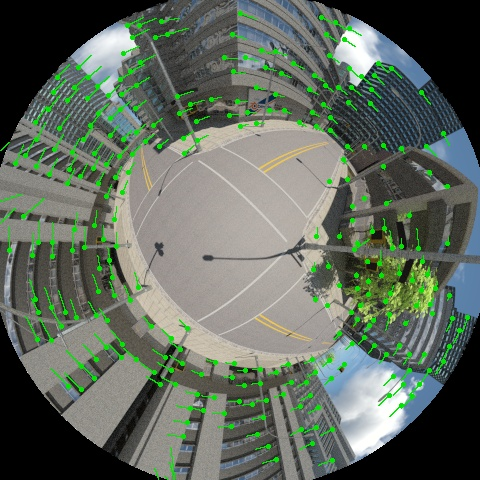
\includegraphics[width=\textwidth]{./figures/robot/method_systemstructure_features.jpg}
    \caption{Urban canyon scenario.}
    \label{fig:robot_experiments_simulation_urbancanyon}
  \end{subfigure}\hfill
  \begin{subfigure}[]{0.475\textwidth}
    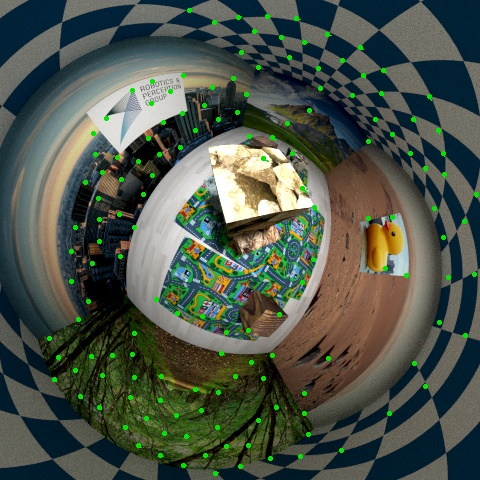
\includegraphics[width=\textwidth]{./figures/robot/indoor_features.jpg}
    \caption{Indoor scenario.}
    \label{fig:robot_experiments_simulation_indoor}
  \end{subfigure}
  \caption{Urban canyon and indoor scenario with sparse optical flow (visualized as green dots and lines).}
  \label{fig:robot_experiments_simulation}
\end{figure}

\begin{figure}[]
  \centering
  \begin{subfigure}[]{\textwidth}
    \centering
    \begin{tikzpicture}[gnuplot]
%% generated with GNUPLOT 5.2p2 (Gentoo revision r0) (Lua 5.1; terminal rev. 99, script rev. 102)
%% Wed 13 Jun 2018 09:57:15 AM CEST
\gpcolor{color=gp lt color axes}
\gpsetlinetype{gp lt axes}
\gpsetdashtype{gp dt axes}
\gpsetlinewidth{0.50}
\draw[gp path] (1.724,1.262)--(9.724,1.262);
\gpcolor{color=gp lt color border}
\gpsetlinetype{gp lt border}
\gpsetdashtype{gp dt solid}
\gpsetlinewidth{1.00}
\draw[gp path] (1.724,1.262)--(1.959,1.262);
\node[gp node right] at (1.530,1.262) {$-20$};
\gpcolor{color=gp lt color axes}
\gpsetlinetype{gp lt axes}
\gpsetdashtype{gp dt axes}
\gpsetlinewidth{0.50}
\draw[gp path] (1.724,2.737)--(9.724,2.737);
\gpcolor{color=gp lt color border}
\gpsetlinetype{gp lt border}
\gpsetdashtype{gp dt solid}
\gpsetlinewidth{1.00}
\draw[gp path] (1.724,2.737)--(1.959,2.737);
\node[gp node right] at (1.530,2.737) {$20$};
\gpcolor{color=gp lt color axes}
\gpsetlinetype{gp lt axes}
\gpsetdashtype{gp dt axes}
\gpsetlinewidth{0.50}
\draw[gp path] (1.724,4.212)--(9.724,4.212);
\gpcolor{color=gp lt color border}
\gpsetlinetype{gp lt border}
\gpsetdashtype{gp dt solid}
\gpsetlinewidth{1.00}
\draw[gp path] (1.724,4.212)--(1.959,4.212);
\node[gp node right] at (1.530,4.212) {$60$};
\gpcolor{color=gp lt color axes}
\gpsetlinetype{gp lt axes}
\gpsetdashtype{gp dt axes}
\gpsetlinewidth{0.50}
\draw[gp path] (1.724,5.687)--(9.724,5.687);
\gpcolor{color=gp lt color border}
\gpsetlinetype{gp lt border}
\gpsetdashtype{gp dt solid}
\gpsetlinewidth{1.00}
\draw[gp path] (1.724,5.687)--(1.959,5.687);
\node[gp node right] at (1.530,5.687) {$100$};
\gpcolor{color=gp lt color axes}
\gpsetlinetype{gp lt axes}
\gpsetdashtype{gp dt axes}
\gpsetlinewidth{0.50}
\draw[gp path] (1.724,7.162)--(9.724,7.162);
\gpcolor{color=gp lt color border}
\gpsetlinetype{gp lt border}
\gpsetdashtype{gp dt solid}
\gpsetlinewidth{1.00}
\draw[gp path] (1.724,7.162)--(1.959,7.162);
\node[gp node right] at (1.530,7.162) {$140$};
\gpcolor{color=gp lt color axes}
\gpsetlinetype{gp lt axes}
\gpsetdashtype{gp dt axes}
\gpsetlinewidth{0.50}
\draw[gp path] (2.451,1.262)--(2.451,7.162);
\gpcolor{color=gp lt color border}
\gpsetlinetype{gp lt border}
\gpsetdashtype{gp dt solid}
\gpsetlinewidth{1.00}
\draw[gp path] (2.451,1.262)--(2.451,1.492);
\node[gp node center] at (2.451,0.867) {$0$};
\gpcolor{color=gp lt color axes}
\gpsetlinetype{gp lt axes}
\gpsetdashtype{gp dt axes}
\gpsetlinewidth{0.50}
\draw[gp path] (3.905,1.262)--(3.905,7.162);
\gpcolor{color=gp lt color border}
\gpsetlinetype{gp lt border}
\gpsetdashtype{gp dt solid}
\gpsetlinewidth{1.00}
\draw[gp path] (3.905,1.262)--(3.905,1.492);
\node[gp node center] at (3.905,0.867) {$40$};
\gpcolor{color=gp lt color axes}
\gpsetlinetype{gp lt axes}
\gpsetdashtype{gp dt axes}
\gpsetlinewidth{0.50}
\draw[gp path] (5.360,1.262)--(5.360,7.162);
\gpcolor{color=gp lt color border}
\gpsetlinetype{gp lt border}
\gpsetdashtype{gp dt solid}
\gpsetlinewidth{1.00}
\draw[gp path] (5.360,1.262)--(5.360,1.492);
\node[gp node center] at (5.360,0.867) {$80$};
\gpcolor{color=gp lt color axes}
\gpsetlinetype{gp lt axes}
\gpsetdashtype{gp dt axes}
\gpsetlinewidth{0.50}
\draw[gp path] (6.814,1.262)--(6.814,7.162);
\gpcolor{color=gp lt color border}
\gpsetlinetype{gp lt border}
\gpsetdashtype{gp dt solid}
\gpsetlinewidth{1.00}
\draw[gp path] (6.814,1.262)--(6.814,1.492);
\node[gp node center] at (6.814,0.867) {$120$};
\gpcolor{color=gp lt color axes}
\gpsetlinetype{gp lt axes}
\gpsetdashtype{gp dt axes}
\gpsetlinewidth{0.50}
\draw[gp path] (8.269,1.262)--(8.269,7.162);
\gpcolor{color=gp lt color border}
\gpsetlinetype{gp lt border}
\gpsetdashtype{gp dt solid}
\gpsetlinewidth{1.00}
\draw[gp path] (8.269,1.262)--(8.269,1.492);
\node[gp node center] at (8.269,0.867) {$160$};
\draw[gp path] (1.724,7.162)--(1.724,1.262)--(9.724,1.262)--(9.724,7.162)--cycle;
\node[gp node center,rotate=-270] at (0.601,4.212) {y [m]};
\node[gp node center] at (5.723,0.275) {x [m]};
\gpcolor{rgb color={0.000,0.667,0.000}}
\gpsetlinewidth{3.00}
\draw[gp path] (2.451,2.000)--(2.452,2.011)--(2.453,2.023)--(2.455,2.034)--(2.455,2.044)%
  --(2.456,2.055)--(2.457,2.065)--(2.457,2.075)--(2.459,2.084)--(2.459,2.093)--(2.460,2.102)%
  --(2.460,2.111)--(2.461,2.119)--(2.463,2.128)--(2.463,2.135)--(2.464,2.143)--(2.464,2.152)%
  --(2.465,2.160)--(2.465,2.167)--(2.466,2.175)--(2.466,2.183)--(2.468,2.190)--(2.468,2.198)%
  --(2.469,2.206)--(2.470,2.213)--(2.470,2.220)--(2.470,2.228)--(2.472,2.235)--(2.473,2.242)%
  --(2.473,2.249)--(2.474,2.256)--(2.474,2.262)--(2.476,2.269)--(2.476,2.275)--(2.477,2.281)%
  --(2.477,2.288)--(2.477,2.294)--(2.478,2.301)--(2.478,2.307)--(2.478,2.312)--(2.478,2.318)%
  --(2.480,2.324)--(2.480,2.330)--(2.480,2.335)--(2.481,2.340)--(2.481,2.345)--(2.481,2.352)%
  --(2.481,2.357)--(2.481,2.363)--(2.482,2.368)--(2.482,2.375)--(2.482,2.380)--(2.483,2.386)%
  --(2.483,2.393)--(2.483,2.399)--(2.483,2.406)--(2.485,2.412)--(2.485,2.418)--(2.485,2.425)%
  --(2.485,2.431)--(2.485,2.438)--(2.485,2.445)--(2.486,2.452)--(2.486,2.458)--(2.486,2.466)%
  --(2.486,2.472)--(2.487,2.480)--(2.487,2.488)--(2.487,2.494)--(2.487,2.502)--(2.487,2.509)%
  --(2.489,2.517)--(2.489,2.525)--(2.489,2.532)--(2.489,2.539)--(2.489,2.547)--(2.489,2.553)%
  --(2.489,2.561)--(2.489,2.567)--(2.489,2.573)--(2.490,2.580)--(2.490,2.586)--(2.490,2.593)%
  --(2.490,2.599)--(2.490,2.605)--(2.490,2.612)--(2.490,2.617)--(2.490,2.623)--(2.490,2.628)%
  --(2.491,2.635)--(2.491,2.640)--(2.491,2.645)--(2.491,2.652)--(2.491,2.657)--(2.491,2.662)%
  --(2.493,2.667)--(2.493,2.671)--(2.493,2.676)--(2.493,2.681)--(2.493,2.686)--(2.493,2.690)%
  --(2.493,2.695)--(2.493,2.699)--(2.493,2.704)--(2.494,2.708)--(2.494,2.713)--(2.494,2.717)%
  --(2.494,2.722)--(2.494,2.726)--(2.494,2.731)--(2.494,2.735)--(2.494,2.740)--(2.494,2.745)%
  --(2.494,2.750)--(2.494,2.757)--(2.494,2.763)--(2.494,2.769)--(2.494,2.776)--(2.494,2.783)%
  --(2.494,2.791)--(2.494,2.799)--(2.494,2.807)--(2.494,2.814)--(2.494,2.822)--(2.494,2.828)%
  --(2.494,2.836)--(2.494,2.844)--(2.494,2.851)--(2.494,2.858)--(2.493,2.864)--(2.493,2.872)%
  --(2.493,2.878)--(2.493,2.885)--(2.493,2.891)--(2.493,2.896)--(2.493,2.903)--(2.493,2.909)%
  --(2.493,2.915)--(2.493,2.921)--(2.493,2.927)--(2.493,2.932)--(2.493,2.938)--(2.493,2.944)%
  --(2.493,2.950)--(2.493,2.955)--(2.493,2.960)--(2.493,2.965)--(2.493,2.970)--(2.493,2.976)%
  --(2.493,2.981)--(2.493,2.986)--(2.493,2.990)--(2.493,2.995)--(2.493,3.000)--(2.493,3.006)%
  --(2.491,3.011)--(2.493,3.017)--(2.491,3.022)--(2.493,3.028)--(2.493,3.035)--(2.493,3.040)%
  --(2.491,3.046)--(2.491,3.052)--(2.491,3.059)--(2.491,3.065)--(2.491,3.072)--(2.491,3.078)%
  --(2.491,3.084)--(2.491,3.092)--(2.491,3.099)--(2.490,3.106)--(2.490,3.113)--(2.490,3.120)%
  --(2.490,3.128)--(2.489,3.134)--(2.489,3.142)--(2.489,3.150)--(2.489,3.156)--(2.487,3.164)%
  --(2.487,3.170)--(2.487,3.178)--(2.487,3.184)--(2.487,3.192)--(2.486,3.199)--(2.486,3.205)%
  --(2.486,3.211)--(2.486,3.218)--(2.485,3.224)--(2.485,3.231)--(2.485,3.237)--(2.485,3.243)%
  --(2.485,3.250)--(2.483,3.255)--(2.483,3.261)--(2.483,3.266)--(2.483,3.273)--(2.483,3.278)%
  --(2.483,3.284)--(2.483,3.289)--(2.482,3.295)--(2.482,3.300)--(2.482,3.305)--(2.482,3.310)%
  --(2.482,3.315)--(2.482,3.320)--(2.482,3.325)--(2.482,3.330)--(2.482,3.336)--(2.482,3.341)%
  --(2.482,3.346)--(2.482,3.351)--(2.481,3.356)--(2.481,3.360)--(2.481,3.365)--(2.481,3.370)%
  --(2.481,3.375)--(2.481,3.379)--(2.481,3.384)--(2.481,3.389)--(2.481,3.394)--(2.481,3.401)%
  --(2.481,3.406)--(2.480,3.412)--(2.480,3.418)--(2.480,3.424)--(2.480,3.429)--(2.480,3.435)%
  --(2.480,3.442)--(2.480,3.448)--(2.480,3.455)--(2.480,3.461)--(2.478,3.467)--(2.478,3.474)%
  --(2.478,3.480)--(2.478,3.487)--(2.478,3.492)--(2.478,3.498)--(2.477,3.505)--(2.477,3.510)%
  --(2.477,3.516)--(2.477,3.521)--(2.477,3.526)--(2.477,3.533)--(2.477,3.538)--(2.477,3.543)%
  --(2.476,3.548)--(2.476,3.553)--(2.476,3.558)--(2.476,3.564)--(2.476,3.569)--(2.476,3.574)%
  --(2.476,3.579)--(2.476,3.584)--(2.476,3.588)--(2.476,3.593)--(2.476,3.598)--(2.476,3.603)%
  --(2.474,3.608)--(2.474,3.614)--(2.474,3.619)--(2.474,3.624)--(2.474,3.629)--(2.474,3.634)%
  --(2.474,3.639)--(2.474,3.643)--(2.474,3.648)--(2.473,3.653)--(2.473,3.657)--(2.473,3.662)%
  --(2.473,3.667)--(2.473,3.672)--(2.473,3.676)--(2.473,3.681)--(2.472,3.687)--(2.472,3.692)%
  --(2.472,3.697)--(2.472,3.703)--(2.472,3.708)--(2.472,3.713)--(2.472,3.720)--(2.472,3.725)%
  --(2.472,3.731)--(2.470,3.736)--(2.470,3.743)--(2.470,3.749)--(2.470,3.756)--(2.470,3.762)%
  --(2.470,3.769)--(2.470,3.775)--(2.470,3.781)--(2.469,3.788)--(2.469,3.794)--(2.469,3.801)%
  --(2.469,3.807)--(2.469,3.813)--(2.469,3.820)--(2.469,3.826)--(2.468,3.833)--(2.468,3.839)%
  --(2.468,3.845)--(2.468,3.852)--(2.468,3.858)--(2.468,3.865)--(2.468,3.871)--(2.466,3.877)%
  --(2.466,3.884)--(2.466,3.890)--(2.466,3.897)--(2.465,3.904)--(2.465,3.911)--(2.465,3.917)%
  --(2.464,3.925)--(2.464,3.932)--(2.464,3.939)--(2.463,3.947)--(2.463,3.954)--(2.463,3.962)%
  --(2.461,3.970)--(2.461,3.977)--(2.461,3.985)--(2.461,3.993)--(2.460,4.000)--(2.460,4.007)%
  --(2.460,4.014)--(2.460,4.021)--(2.460,4.029)--(2.459,4.035)--(2.459,4.043)--(2.459,4.049)%
  --(2.459,4.057)--(2.459,4.063)--(2.457,4.071)--(2.457,4.077)--(2.457,4.085)--(2.457,4.091)%
  --(2.456,4.098)--(2.456,4.105)--(2.456,4.112)--(2.456,4.119)--(2.456,4.127)--(2.456,4.135)%
  --(2.455,4.144)--(2.455,4.152)--(2.455,4.160)--(2.455,4.168)--(2.453,4.177)--(2.453,4.185)%
  --(2.453,4.194)--(2.452,4.203)--(2.452,4.210)--(2.452,4.219)--(2.452,4.228)--(2.451,4.237)%
  --(2.451,4.246)--(2.451,4.254)--(2.451,4.263)--(2.451,4.271)--(2.451,4.280)--(2.451,4.287)%
  --(2.451,4.295)--(2.449,4.303)--(2.449,4.310)--(2.449,4.318)--(2.449,4.326)--(2.449,4.333)%
  --(2.449,4.341)--(2.449,4.349)--(2.449,4.356)--(2.449,4.364)--(2.449,4.372)--(2.448,4.380)%
  --(2.449,4.387)--(2.449,4.395)--(2.449,4.403)--(2.449,4.410)--(2.449,4.418)--(2.449,4.426)%
  --(2.449,4.432)--(2.449,4.440)--(2.451,4.447)--(2.451,4.455)--(2.452,4.463)--(2.452,4.469)%
  --(2.453,4.477)--(2.455,4.485)--(2.456,4.492)--(2.457,4.500)--(2.459,4.506)--(2.460,4.514)%
  --(2.461,4.522)--(2.463,4.529)--(2.464,4.536)--(2.465,4.542)--(2.466,4.550)--(2.469,4.556)%
  --(2.472,4.563)--(2.474,4.570)--(2.477,4.577)--(2.480,4.584)--(2.482,4.591)--(2.486,4.597)%
  --(2.489,4.604)--(2.490,4.611)--(2.493,4.619)--(2.495,4.625)--(2.498,4.633)--(2.500,4.640)%
  --(2.504,4.646)--(2.508,4.654)--(2.512,4.660)--(2.517,4.666)--(2.523,4.673)--(2.528,4.679)%
  --(2.533,4.686)--(2.540,4.692)--(2.545,4.698)--(2.549,4.706)--(2.554,4.714)--(2.559,4.722)%
  --(2.566,4.729)--(2.571,4.736)--(2.577,4.743)--(2.585,4.750)--(2.592,4.756)--(2.598,4.761)%
  --(2.606,4.768)--(2.614,4.773)--(2.622,4.778)--(2.630,4.782)--(2.638,4.787)--(2.643,4.792)%
  --(2.649,4.797)--(2.656,4.802)--(2.662,4.807)--(2.669,4.811)--(2.675,4.815)--(2.682,4.820)%
  --(2.688,4.823)--(2.695,4.827)--(2.700,4.829)--(2.707,4.830)--(2.712,4.833)--(2.717,4.834)%
  --(2.724,4.837)--(2.729,4.839)--(2.734,4.842)--(2.739,4.845)--(2.746,4.847)--(2.751,4.850)%
  --(2.756,4.851)--(2.763,4.853)--(2.769,4.855)--(2.775,4.856)--(2.781,4.857)--(2.788,4.859)%
  --(2.793,4.860)--(2.799,4.861)--(2.806,4.862)--(2.812,4.864)--(2.818,4.866)--(2.826,4.868)%
  --(2.832,4.869)--(2.839,4.870)--(2.845,4.871)--(2.852,4.873)--(2.858,4.874)--(2.863,4.874)%
  --(2.870,4.875)--(2.876,4.875)--(2.883,4.877)--(2.890,4.877)--(2.896,4.878)--(2.903,4.878)%
  --(2.909,4.879)--(2.916,4.879)--(2.923,4.880)--(2.930,4.880)--(2.938,4.880)--(2.944,4.882)%
  --(2.952,4.882)--(2.959,4.882)--(2.967,4.882)--(2.973,4.882)--(2.981,4.882)--(2.989,4.882)%
  --(2.997,4.882)--(3.003,4.882)--(3.011,4.882)--(3.019,4.882)--(3.025,4.882)--(3.033,4.882)%
  --(3.040,4.882)--(3.046,4.882)--(3.053,4.882)--(3.059,4.882)--(3.067,4.880)--(3.074,4.880)%
  --(3.080,4.879)--(3.088,4.879)--(3.094,4.879)--(3.102,4.878)--(3.109,4.878)--(3.117,4.878)%
  --(3.123,4.877)--(3.130,4.877)--(3.136,4.877)--(3.143,4.875)--(3.149,4.875)--(3.157,4.875)%
  --(3.164,4.874)--(3.169,4.874)--(3.175,4.874)--(3.182,4.873)--(3.189,4.873)--(3.195,4.871)%
  --(3.202,4.871)--(3.208,4.871)--(3.215,4.870)--(3.221,4.870)--(3.228,4.870)--(3.234,4.870)%
  --(3.241,4.869)--(3.247,4.869)--(3.254,4.869)--(3.259,4.868)--(3.264,4.868)--(3.271,4.868)%
  --(3.277,4.866)--(3.284,4.866)--(3.290,4.865)--(3.297,4.865)--(3.303,4.864)--(3.310,4.862)%
  --(3.318,4.862)--(3.324,4.861)--(3.332,4.860)--(3.339,4.859)--(3.345,4.857)--(3.353,4.857)%
  --(3.360,4.856)--(3.367,4.855)--(3.375,4.853)--(3.384,4.852)--(3.392,4.851)--(3.401,4.848)%
  --(3.409,4.846)--(3.418,4.843)--(3.426,4.841)--(3.435,4.837)--(3.443,4.833)--(3.451,4.829)%
  --(3.459,4.824)--(3.467,4.819)--(3.474,4.814)--(3.482,4.810)--(3.489,4.809)--(3.495,4.806)%
  --(3.502,4.804)--(3.507,4.801)--(3.514,4.797)--(3.519,4.792)--(3.524,4.788)--(3.529,4.783)%
  --(3.535,4.777)--(3.538,4.771)--(3.542,4.765)--(3.545,4.759)--(3.549,4.752)--(3.553,4.747)%
  --(3.558,4.742)--(3.563,4.737)--(3.567,4.731)--(3.572,4.725)--(3.576,4.718)--(3.579,4.711)%
  --(3.583,4.704)--(3.585,4.697)--(3.588,4.690)--(3.589,4.681)--(3.591,4.674)--(3.591,4.666)%
  --(3.591,4.659)--(3.593,4.650)--(3.596,4.642)--(3.598,4.634)--(3.601,4.625)--(3.602,4.617)%
  --(3.604,4.606)--(3.606,4.597)--(3.608,4.587)--(3.609,4.577)--(3.610,4.568)--(3.610,4.558)%
  --(3.610,4.549)--(3.610,4.538)--(3.610,4.529)--(3.612,4.520)--(3.612,4.511)--(3.613,4.502)%
  --(3.613,4.494)--(3.613,4.485)--(3.613,4.477)--(3.613,4.468)--(3.613,4.460)--(3.613,4.453)%
  --(3.613,4.446)--(3.613,4.438)--(3.613,4.432)--(3.613,4.426)--(3.612,4.418)--(3.612,4.412)%
  --(3.612,4.404)--(3.612,4.397)--(3.610,4.391)--(3.610,4.385)--(3.610,4.378)--(3.610,4.371)%
  --(3.610,4.364)--(3.610,4.356)--(3.610,4.350)--(3.610,4.342)--(3.609,4.335)--(3.609,4.327)%
  --(3.609,4.321)--(3.609,4.313)--(3.609,4.307)--(3.609,4.300)--(3.609,4.294)--(3.610,4.287)%
  --(3.610,4.281)--(3.610,4.274)--(3.612,4.268)--(3.612,4.262)--(3.613,4.254)--(3.613,4.248)%
  --(3.614,4.241)--(3.615,4.233)--(3.617,4.226)--(3.617,4.218)--(3.618,4.210)--(3.619,4.203)%
  --(3.621,4.195)--(3.622,4.187)--(3.625,4.178)--(3.627,4.171)--(3.630,4.163)--(3.634,4.157)%
  --(3.636,4.149)--(3.640,4.141)--(3.644,4.135)--(3.648,4.128)--(3.651,4.122)--(3.652,4.116)%
  --(3.653,4.108)--(3.655,4.102)--(3.657,4.095)--(3.661,4.089)--(3.664,4.082)--(3.669,4.076)%
  --(3.674,4.071)--(3.679,4.064)--(3.685,4.059)--(3.691,4.054)--(3.698,4.050)--(3.704,4.046)%
  --(3.709,4.043)--(3.715,4.038)--(3.720,4.032)--(3.725,4.026)--(3.732,4.021)--(3.738,4.017)%
  --(3.745,4.012)--(3.751,4.008)--(3.758,4.003)--(3.766,4.000)--(3.772,3.997)--(3.780,3.993)%
  --(3.788,3.990)--(3.796,3.989)--(3.803,3.986)--(3.811,3.982)--(3.819,3.980)--(3.827,3.977)%
  --(3.835,3.973)--(3.841,3.972)--(3.849,3.970)--(3.856,3.967)--(3.864,3.966)--(3.871,3.963)%
  --(3.879,3.961)--(3.888,3.959)--(3.896,3.958)--(3.904,3.957)--(3.912,3.954)--(3.921,3.952)%
  --(3.929,3.949)--(3.937,3.948)--(3.945,3.945)--(3.952,3.944)--(3.960,3.943)--(3.968,3.941)%
  --(3.976,3.940)--(3.984,3.940)--(3.992,3.939)--(3.999,3.939)--(4.007,3.939)--(4.015,3.939)%
  --(4.023,3.938)--(4.029,3.938)--(4.036,3.936)--(4.044,3.936)--(4.052,3.936)--(4.059,3.936)%
  --(4.069,3.938)--(4.076,3.938)--(4.086,3.939)--(4.095,3.940)--(4.104,3.941)--(4.113,3.944)%
  --(4.122,3.945)--(4.131,3.948)--(4.142,3.949)--(4.151,3.950)--(4.161,3.952)--(4.170,3.953)%
  --(4.181,3.956)--(4.190,3.958)--(4.199,3.961)--(4.208,3.962)--(4.217,3.966)--(4.227,3.968)%
  --(4.234,3.971)--(4.244,3.975)--(4.253,3.980)--(4.262,3.984)--(4.271,3.986)--(4.281,3.990)%
  --(4.292,3.994)--(4.302,3.998)--(4.313,4.002)--(4.323,4.007)--(4.334,4.012)--(4.345,4.018)%
  --(4.356,4.023)--(4.365,4.030)--(4.374,4.035)--(4.382,4.040)--(4.390,4.045)--(4.398,4.052)%
  --(4.405,4.055)--(4.413,4.061)--(4.420,4.066)--(4.428,4.071)--(4.434,4.076)--(4.441,4.081)%
  --(4.447,4.086)--(4.454,4.093)--(4.459,4.098)--(4.464,4.104)--(4.469,4.111)--(4.475,4.116)%
  --(4.480,4.122)--(4.484,4.128)--(4.489,4.134)--(4.496,4.139)--(4.501,4.144)--(4.506,4.150)%
  --(4.510,4.157)--(4.515,4.163)--(4.519,4.169)--(4.523,4.176)--(4.526,4.184)--(4.528,4.191)%
  --(4.531,4.199)--(4.533,4.207)--(4.535,4.214)--(4.536,4.222)--(4.540,4.228)--(4.544,4.236)%
  --(4.546,4.242)--(4.550,4.250)--(4.553,4.258)--(4.556,4.266)--(4.558,4.273)--(4.559,4.281)%
  --(4.562,4.289)--(4.563,4.296)--(4.565,4.304)--(4.566,4.312)--(4.567,4.321)--(4.569,4.328)%
  --(4.570,4.336)--(4.573,4.345)--(4.574,4.353)--(4.575,4.360)--(4.576,4.369)--(4.578,4.377)%
  --(4.579,4.385)--(4.579,4.392)--(4.580,4.401)--(4.580,4.409)--(4.582,4.417)--(4.582,4.424)%
  --(4.580,4.432)--(4.582,4.440)--(4.582,4.447)--(4.582,4.455)--(4.582,4.464)--(4.582,4.472)%
  --(4.582,4.481)--(4.582,4.491)--(4.580,4.501)--(4.580,4.511)--(4.579,4.523)--(4.578,4.535)%
  --(4.575,4.547)--(4.574,4.560)--(4.571,4.573)--(4.570,4.586)--(4.569,4.600)--(4.567,4.613)%
  --(4.566,4.627)--(4.565,4.640)--(4.562,4.652)--(4.559,4.664)--(4.557,4.677)--(4.554,4.688)%
  --(4.552,4.700)--(4.548,4.711)--(4.545,4.723)--(4.541,4.734)--(4.539,4.745)--(4.535,4.756)%
  --(4.532,4.766)--(4.529,4.775)--(4.526,4.786)--(4.523,4.796)--(4.519,4.805)--(4.515,4.814)%
  --(4.511,4.824)--(4.507,4.833)--(4.502,4.842)--(4.498,4.851)--(4.493,4.860)--(4.488,4.869)%
  --(4.482,4.878)--(4.479,4.888)--(4.475,4.898)--(4.471,4.907)--(4.465,4.916)--(4.460,4.925)%
  --(4.455,4.933)--(4.450,4.941)--(4.445,4.947)--(4.438,4.953)--(4.432,4.960)--(4.425,4.966)%
  --(4.418,4.971)--(4.412,4.976)--(4.407,4.980)--(4.402,4.987)--(4.398,4.992)--(4.394,4.997)%
  --(4.388,5.002)--(4.383,5.007)--(4.379,5.011)--(4.374,5.015)--(4.369,5.017)--(4.362,5.021)%
  --(4.357,5.024)--(4.351,5.026)--(4.345,5.028)--(4.339,5.029)--(4.334,5.030)--(4.327,5.034)%
  --(4.322,5.037)--(4.315,5.039)--(4.310,5.042)--(4.304,5.043)--(4.297,5.046)--(4.291,5.048)%
  --(4.284,5.049)--(4.277,5.051)--(4.271,5.052)--(4.266,5.053)--(4.259,5.053)--(4.253,5.055)%
  --(4.246,5.055)--(4.240,5.056)--(4.233,5.057)--(4.227,5.057)--(4.220,5.058)--(4.212,5.060)%
  --(4.206,5.060)--(4.199,5.061)--(4.191,5.061)--(4.185,5.061)--(4.177,5.062)--(4.170,5.062)%
  --(4.164,5.062)--(4.156,5.061)--(4.148,5.061)--(4.140,5.062)--(4.134,5.062)--(4.126,5.062)%
  --(4.118,5.062)--(4.110,5.062)--(4.102,5.062)--(4.096,5.062)--(4.088,5.062)--(4.082,5.062)%
  --(4.074,5.062)--(4.066,5.061)--(4.058,5.061)--(4.050,5.060)--(4.042,5.060)--(4.036,5.058)%
  --(4.029,5.058)--(4.024,5.058)--(4.018,5.057)--(4.012,5.057)--(4.007,5.057)--(4.001,5.056)%
  --(3.994,5.056)--(3.989,5.056)--(3.982,5.055)--(3.976,5.053)--(3.969,5.053)--(3.963,5.052)%
  --(3.956,5.051)--(3.950,5.051)--(3.942,5.049)--(3.935,5.048)--(3.928,5.048)--(3.920,5.047)%
  --(3.913,5.046)--(3.905,5.044)--(3.898,5.043)--(3.890,5.042)--(3.882,5.042)--(3.874,5.040)%
  --(3.866,5.039)--(3.858,5.038)--(3.850,5.037)--(3.843,5.035)--(3.835,5.034)--(3.827,5.033)%
  --(3.818,5.032)--(3.809,5.029)--(3.800,5.028)--(3.792,5.026)--(3.783,5.024)--(3.773,5.023)%
  --(3.763,5.021)--(3.754,5.019)--(3.745,5.017)--(3.736,5.015)--(3.726,5.014)--(3.717,5.012)%
  --(3.708,5.010)--(3.698,5.008)--(3.689,5.006)--(3.679,5.005)--(3.669,5.002)--(3.660,5.001)%
  --(3.651,4.998)--(3.640,4.996)--(3.631,4.994)--(3.621,4.992)--(3.610,4.989)--(3.601,4.988)%
  --(3.591,4.985)--(3.582,4.983)--(3.571,4.982)--(3.562,4.979)--(3.553,4.978)--(3.542,4.975)%
  --(3.533,4.974)--(3.524,4.971)--(3.516,4.970)--(3.507,4.967)--(3.498,4.966)--(3.489,4.965)%
  --(3.481,4.964)--(3.473,4.961)--(3.464,4.960)--(3.456,4.959)--(3.447,4.957)--(3.438,4.955)%
  --(3.430,4.953)--(3.421,4.952)--(3.413,4.951)--(3.404,4.948)--(3.396,4.947)--(3.388,4.946)%
  --(3.379,4.944)--(3.371,4.943)--(3.363,4.942)--(3.357,4.941)--(3.349,4.938)--(3.341,4.937)%
  --(3.333,4.935)--(3.326,4.934)--(3.319,4.933)--(3.311,4.932)--(3.303,4.930)--(3.297,4.929)%
  --(3.289,4.928)--(3.281,4.926)--(3.275,4.925)--(3.267,4.924)--(3.260,4.923)--(3.252,4.921)%
  --(3.246,4.920)--(3.238,4.919)--(3.232,4.918)--(3.225,4.916)--(3.219,4.915)--(3.211,4.914)%
  --(3.204,4.912)--(3.196,4.911)--(3.189,4.910)--(3.182,4.909)--(3.174,4.907)--(3.168,4.906)%
  --(3.160,4.905)--(3.153,4.903)--(3.145,4.902)--(3.139,4.901)--(3.132,4.900)--(3.126,4.898)%
  --(3.118,4.898)--(3.111,4.897)--(3.105,4.896)--(3.098,4.894)--(3.092,4.893)--(3.085,4.893)%
  --(3.079,4.892)--(3.072,4.891)--(3.066,4.889)--(3.059,4.889)--(3.053,4.888)--(3.046,4.887)%
  --(3.040,4.885)--(3.034,4.885)--(3.028,4.884)--(3.021,4.883)--(3.015,4.882)--(3.008,4.882)%
  --(3.002,4.880)--(2.995,4.879)--(2.990,4.878)--(2.984,4.878)--(2.977,4.877)--(2.969,4.875)%
  --(2.963,4.874)--(2.956,4.873)--(2.950,4.873)--(2.943,4.871)--(2.935,4.870)--(2.929,4.870)%
  --(2.921,4.869)--(2.914,4.868)--(2.906,4.866)--(2.900,4.866)--(2.892,4.865)--(2.886,4.864)%
  --(2.878,4.864)--(2.870,4.862)--(2.862,4.861)--(2.854,4.860)--(2.846,4.859)--(2.839,4.859)%
  --(2.831,4.857)--(2.822,4.857)--(2.814,4.856)--(2.805,4.856)--(2.795,4.856)--(2.786,4.856)%
  --(2.777,4.856)--(2.769,4.855)--(2.760,4.856)--(2.751,4.855)--(2.743,4.855)--(2.734,4.855)%
  --(2.726,4.853)--(2.718,4.855)--(2.709,4.855)--(2.701,4.855)--(2.694,4.856)--(2.685,4.857)%
  --(2.677,4.859)--(2.669,4.860)--(2.661,4.861)--(2.653,4.862)--(2.645,4.865)--(2.636,4.866)%
  --(2.627,4.866)--(2.619,4.868)--(2.610,4.870)--(2.601,4.871)--(2.593,4.874)--(2.585,4.878)%
  --(2.577,4.880)--(2.570,4.884)--(2.563,4.888)--(2.557,4.892)--(2.550,4.897)--(2.543,4.902)%
  --(2.537,4.907)--(2.530,4.911)--(2.523,4.914)--(2.516,4.918)--(2.510,4.921)--(2.503,4.926)%
  --(2.496,4.932)--(2.491,4.937)--(2.486,4.943)--(2.481,4.950)--(2.477,4.956)--(2.473,4.962)%
  --(2.469,4.970)--(2.466,4.978)--(2.464,4.985)--(2.460,4.991)--(2.455,4.997)--(2.449,5.003)%
  --(2.446,5.010)--(2.442,5.016)--(2.438,5.024)--(2.435,5.030)--(2.433,5.037)--(2.430,5.044)%
  --(2.427,5.052)--(2.425,5.060)--(2.423,5.067)--(2.422,5.075)--(2.421,5.083)--(2.418,5.090)%
  --(2.416,5.098)--(2.414,5.106)--(2.412,5.114)--(2.410,5.121)--(2.408,5.129)--(2.406,5.137)%
  --(2.405,5.144)--(2.404,5.152)--(2.402,5.160)--(2.401,5.167)--(2.400,5.174)--(2.399,5.181)%
  --(2.397,5.189)--(2.396,5.195)--(2.395,5.203)--(2.393,5.210)--(2.392,5.217)--(2.391,5.224)%
  --(2.391,5.230)--(2.389,5.238)--(2.388,5.244)--(2.387,5.252)--(2.386,5.260)--(2.386,5.267)%
  --(2.384,5.275)--(2.383,5.281)--(2.383,5.289)--(2.382,5.295)--(2.380,5.303)--(2.379,5.309)%
  --(2.379,5.317)--(2.378,5.324)--(2.376,5.331)--(2.376,5.339)--(2.375,5.345)--(2.375,5.353)%
  --(2.374,5.361)--(2.374,5.368)--(2.372,5.376)--(2.372,5.384)--(2.371,5.391)--(2.370,5.398)%
  --(2.370,5.406)--(2.369,5.412)--(2.369,5.420)--(2.367,5.426)--(2.367,5.432)--(2.366,5.439)%
  --(2.366,5.445)--(2.365,5.452)--(2.365,5.458)--(2.363,5.464)--(2.363,5.471)--(2.363,5.476)%
  --(2.362,5.482)--(2.362,5.489)--(2.361,5.494)--(2.361,5.500)--(2.359,5.505)--(2.359,5.512)%
  --(2.358,5.518)--(2.358,5.523)--(2.357,5.530)--(2.357,5.535)--(2.355,5.541)--(2.355,5.548)%
  --(2.355,5.554)--(2.354,5.562)--(2.354,5.568)--(2.353,5.575)--(2.353,5.581)--(2.352,5.589)%
  --(2.352,5.596)--(2.350,5.603)--(2.350,5.611)--(2.349,5.618)--(2.349,5.625)--(2.349,5.632)%
  --(2.348,5.639)--(2.348,5.645)--(2.346,5.653)--(2.346,5.659)--(2.345,5.667)--(2.345,5.673)%
  --(2.345,5.680)--(2.344,5.686)--(2.344,5.692)--(2.342,5.699)--(2.342,5.705)--(2.342,5.712)%
  --(2.341,5.718)--(2.341,5.725)--(2.340,5.730)--(2.340,5.736)--(2.339,5.742)--(2.339,5.748)%
  --(2.339,5.753)--(2.337,5.759)--(2.337,5.764)--(2.336,5.769)--(2.336,5.776)--(2.336,5.781)%
  --(2.335,5.786)--(2.335,5.791)--(2.335,5.796)--(2.333,5.801)--(2.333,5.806)--(2.333,5.812)%
  --(2.332,5.817)--(2.332,5.822)--(2.331,5.827)--(2.331,5.831)--(2.331,5.836)--(2.329,5.841)%
  --(2.329,5.845)--(2.329,5.850)--(2.328,5.854)--(2.328,5.859)--(2.328,5.863)--(2.328,5.868)%
  --(2.327,5.872)--(2.327,5.876)--(2.327,5.881)--(2.327,5.885)--(2.325,5.890)--(2.325,5.895)%
  --(2.325,5.899)--(2.325,5.904)--(2.325,5.909)--(2.325,5.913)--(2.325,5.918)--(2.325,5.923)%
  --(2.325,5.927)--(2.325,5.932)--(2.327,5.937)--(2.327,5.942)--(2.328,5.947)--(2.328,5.953)%
  --(2.328,5.959)--(2.329,5.965)--(2.329,5.970)--(2.331,5.977)--(2.331,5.983)--(2.332,5.988)%
  --(2.335,5.995)--(2.336,6.000)--(2.337,6.006)--(2.340,6.011)--(2.342,6.018)--(2.345,6.023)%
  --(2.348,6.029)--(2.350,6.034)--(2.352,6.040)--(2.353,6.046)--(2.355,6.051)--(2.357,6.056)%
  --(2.359,6.061)--(2.362,6.067)--(2.366,6.072)--(2.369,6.077)--(2.372,6.081)--(2.376,6.086)%
  --(2.380,6.090)--(2.386,6.095)--(2.391,6.100)--(2.395,6.105)--(2.400,6.113)--(2.404,6.118)%
  --(2.408,6.125)--(2.414,6.132)--(2.419,6.138)--(2.427,6.146)--(2.435,6.155)--(2.446,6.164)%
  --(2.457,6.174)--(2.472,6.183)--(2.485,6.193)--(2.499,6.201)--(2.515,6.210)--(2.528,6.220)%
  --(2.540,6.230)--(2.551,6.239)--(2.563,6.247)--(2.572,6.255)--(2.583,6.261)--(2.593,6.268)%
  --(2.604,6.273)--(2.613,6.278)--(2.623,6.283)--(2.632,6.288)--(2.641,6.292)--(2.652,6.296)%
  --(2.660,6.298)--(2.669,6.303)--(2.677,6.307)--(2.685,6.311)--(2.692,6.315)--(2.701,6.319)%
  --(2.709,6.323)--(2.716,6.325)--(2.724,6.329)--(2.732,6.332)--(2.739,6.334)--(2.746,6.337)%
  --(2.754,6.338)--(2.762,6.341)--(2.768,6.343)--(2.776,6.344)--(2.782,6.347)--(2.790,6.351)%
  --(2.797,6.352)--(2.805,6.355)--(2.811,6.357)--(2.819,6.360)--(2.827,6.361)--(2.833,6.364)%
  --(2.841,6.365)--(2.849,6.368)--(2.857,6.369)--(2.865,6.370)--(2.873,6.373)--(2.879,6.374)%
  --(2.887,6.375)--(2.895,6.378)--(2.903,6.379)--(2.909,6.380)--(2.917,6.382)--(2.923,6.383)%
  --(2.931,6.384)--(2.938,6.385)--(2.946,6.387)--(2.952,6.388)--(2.959,6.389)--(2.965,6.389)%
  --(2.973,6.391)--(2.980,6.392)--(2.986,6.393)--(2.993,6.394)--(2.999,6.394)--(3.006,6.396)%
  --(3.012,6.397)--(3.019,6.398)--(3.024,6.398)--(3.031,6.400)--(3.037,6.400)--(3.044,6.401)%
  --(3.049,6.402)--(3.055,6.402)--(3.062,6.403)--(3.067,6.403)--(3.074,6.405)--(3.080,6.406)%
  --(3.085,6.406)--(3.092,6.407)--(3.098,6.409)--(3.105,6.409)--(3.111,6.410)--(3.118,6.410)%
  --(3.125,6.411)--(3.132,6.412)--(3.140,6.412)--(3.148,6.414)--(3.156,6.415)--(3.164,6.415)%
  --(3.172,6.416)--(3.179,6.417)--(3.189,6.419)--(3.196,6.419)--(3.205,6.420)--(3.215,6.421)%
  --(3.222,6.421)--(3.232,6.423)--(3.239,6.423)--(3.249,6.424)--(3.256,6.424)--(3.264,6.424)%
  --(3.272,6.425)--(3.280,6.425)--(3.288,6.426)--(3.296,6.426)--(3.303,6.428)--(3.310,6.428)%
  --(3.318,6.429)--(3.324,6.430)--(3.332,6.430)--(3.339,6.432)--(3.345,6.432)--(3.353,6.433)%
  --(3.360,6.434)--(3.366,6.434)--(3.373,6.435)--(3.379,6.435)--(3.386,6.437)--(3.392,6.437)%
  --(3.397,6.438)--(3.404,6.438)--(3.410,6.439)--(3.417,6.441)--(3.422,6.441)--(3.429,6.442)%
  --(3.435,6.442)--(3.441,6.443)--(3.447,6.444)--(3.452,6.444)--(3.459,6.446)--(3.465,6.447)%
  --(3.471,6.447)--(3.477,6.448)--(3.484,6.450)--(3.489,6.450)--(3.495,6.451)--(3.502,6.452)%
  --(3.507,6.453)--(3.514,6.453)--(3.519,6.455)--(3.525,6.456)--(3.531,6.456)--(3.536,6.457)%
  --(3.541,6.458)--(3.548,6.458)--(3.553,6.460)--(3.559,6.461)--(3.567,6.462)--(3.574,6.462)%
  --(3.580,6.464)--(3.587,6.465)--(3.595,6.466)--(3.601,6.467)--(3.608,6.469)--(3.614,6.470)%
  --(3.621,6.471)--(3.627,6.473)--(3.634,6.473)--(3.640,6.474)--(3.647,6.475)--(3.653,6.476)%
  --(3.660,6.478)--(3.666,6.479)--(3.672,6.480)--(3.678,6.482)--(3.683,6.482)--(3.690,6.483)%
  --(3.695,6.484)--(3.702,6.485)--(3.707,6.487)--(3.712,6.487)--(3.717,6.488)--(3.723,6.489)%
  --(3.729,6.489)--(3.734,6.491)--(3.740,6.492)--(3.745,6.493)--(3.750,6.494)--(3.755,6.494)%
  --(3.760,6.496)--(3.766,6.497)--(3.771,6.498)--(3.776,6.499)--(3.783,6.499)--(3.788,6.501)%
  --(3.794,6.502)--(3.801,6.503)--(3.806,6.503)--(3.813,6.505)--(3.819,6.506)--(3.826,6.506)%
  --(3.831,6.507)--(3.837,6.507)--(3.844,6.508)--(3.849,6.508)--(3.856,6.508)--(3.862,6.510)%
  --(3.869,6.510)--(3.875,6.511)--(3.882,6.512)--(3.888,6.512)--(3.896,6.514)--(3.903,6.514)%
  --(3.911,6.514)--(3.918,6.514)--(3.925,6.514)--(3.933,6.514)--(3.941,6.512)--(3.947,6.512)%
  --(3.954,6.511)--(3.960,6.511)--(3.967,6.510)--(3.973,6.508)--(3.980,6.508)--(3.986,6.508)%
  --(3.993,6.507)--(3.999,6.506)--(4.006,6.505)--(4.012,6.503)--(4.019,6.501)--(4.024,6.499)%
  --(4.029,6.497)--(4.033,6.494)--(4.039,6.492)--(4.042,6.489)--(4.048,6.487)--(4.053,6.484)%
  --(4.057,6.483)--(4.062,6.480)--(4.067,6.479)--(4.072,6.476)--(4.076,6.474)--(4.082,6.471)%
  --(4.086,6.467)--(4.091,6.464)--(4.095,6.460)--(4.099,6.456)--(4.102,6.451)--(4.106,6.447)%
  --(4.109,6.442)--(4.112,6.438)--(4.117,6.434)--(4.121,6.430)--(4.125,6.425)--(4.129,6.421)%
  --(4.133,6.416)--(4.136,6.411)--(4.140,6.406)--(4.143,6.401)--(4.146,6.394)--(4.150,6.388)%
  --(4.152,6.382)--(4.155,6.374)--(4.156,6.368)--(4.159,6.361)--(4.163,6.355)--(4.165,6.350)%
  --(4.168,6.343)--(4.170,6.337)--(4.173,6.330)--(4.176,6.323)--(4.178,6.316)--(4.181,6.310)%
  --(4.182,6.302)--(4.185,6.295)--(4.186,6.288)--(4.187,6.282)--(4.189,6.274)--(4.190,6.268)%
  --(4.191,6.261)--(4.193,6.255)--(4.194,6.247)--(4.197,6.241)--(4.198,6.234)--(4.199,6.227)%
  --(4.199,6.220)--(4.200,6.213)--(4.202,6.206)--(4.203,6.198)--(4.204,6.192)--(4.204,6.184)%
  --(4.206,6.177)--(4.206,6.169)--(4.207,6.163)--(4.208,6.155)--(4.208,6.149)--(4.210,6.141)%
  --(4.210,6.134)--(4.211,6.127)--(4.211,6.120)--(4.212,6.113)--(4.212,6.106)--(4.212,6.099)%
  --(4.213,6.092)--(4.213,6.084)--(4.213,6.078)--(4.215,6.072)--(4.215,6.065)--(4.215,6.059)%
  --(4.216,6.052)--(4.216,6.047)--(4.216,6.041)--(4.217,6.034)--(4.217,6.029)--(4.217,6.023)%
  --(4.219,6.018)--(4.219,6.013)--(4.219,6.006)--(4.220,6.001)--(4.220,5.996)--(4.220,5.991)%
  --(4.221,5.986)--(4.221,5.982)--(4.221,5.977)--(4.223,5.972)--(4.223,5.967)--(4.224,5.963)%
  --(4.224,5.958)--(4.225,5.953)--(4.225,5.947)--(4.227,5.942)--(4.227,5.937)--(4.228,5.932)%
  --(4.228,5.927)--(4.229,5.922)--(4.229,5.917)--(4.230,5.912)--(4.230,5.906)--(4.232,5.901)%
  --(4.232,5.896)--(4.232,5.891)--(4.233,5.886)--(4.233,5.881)--(4.234,5.876)--(4.234,5.871)%
  --(4.236,5.865)--(4.237,5.860)--(4.237,5.856)--(4.238,5.851)--(4.238,5.846)--(4.240,5.841)%
  --(4.240,5.836)--(4.241,5.831)--(4.242,5.826)--(4.242,5.819)--(4.244,5.813)--(4.245,5.806)%
  --(4.246,5.800)--(4.247,5.794)--(4.249,5.787)--(4.249,5.780)--(4.250,5.773)--(4.251,5.767)%
  --(4.253,5.760)--(4.254,5.753)--(4.255,5.746)--(4.257,5.740)--(4.258,5.733)--(4.259,5.727)%
  --(4.259,5.721)--(4.260,5.714)--(4.262,5.708)--(4.263,5.701)--(4.263,5.696)--(4.264,5.690)%
  --(4.266,5.684)--(4.266,5.678)--(4.267,5.672)--(4.268,5.667)--(4.268,5.662)--(4.270,5.655)%
  --(4.271,5.650)--(4.271,5.645)--(4.272,5.640)--(4.272,5.634)--(4.274,5.628)--(4.275,5.623)%
  --(4.275,5.617)--(4.276,5.612)--(4.276,5.605)--(4.277,5.599)--(4.279,5.593)--(4.279,5.586)%
  --(4.280,5.580)--(4.281,5.573)--(4.281,5.566)--(4.283,5.558)--(4.284,5.552)--(4.285,5.544)%
  --(4.287,5.536)--(4.288,5.529)--(4.288,5.521)--(4.289,5.514)--(4.291,5.508)--(4.292,5.500)%
  --(4.293,5.494)--(4.294,5.486)--(4.294,5.480)--(4.296,5.473)--(4.297,5.467)--(4.297,5.461)%
  --(4.298,5.456)--(4.298,5.449)--(4.300,5.443)--(4.300,5.438)--(4.301,5.431)--(4.301,5.425)%
  --(4.302,5.418)--(4.302,5.413)--(4.304,5.407)--(4.304,5.402)--(4.305,5.395)--(4.305,5.390)%
  --(4.306,5.384)--(4.306,5.379)--(4.307,5.372)--(4.307,5.367)--(4.309,5.361)--(4.309,5.354)%
  --(4.310,5.349)--(4.310,5.343)--(4.311,5.336)--(4.313,5.330)--(4.313,5.322)--(4.314,5.316)%
  --(4.315,5.308)--(4.315,5.301)--(4.317,5.294)--(4.318,5.286)--(4.319,5.279)--(4.319,5.272)%
  --(4.321,5.265)--(4.322,5.257)--(4.323,5.251)--(4.323,5.243)--(4.324,5.235)--(4.326,5.228)%
  --(4.327,5.220)--(4.328,5.212)--(4.328,5.204)--(4.330,5.197)--(4.331,5.189)--(4.332,5.181)%
  --(4.334,5.174)--(4.334,5.166)--(4.335,5.158)--(4.336,5.151)--(4.338,5.143)--(4.338,5.135)%
  --(4.339,5.128)--(4.340,5.121)--(4.341,5.114)--(4.343,5.106)--(4.343,5.098)--(4.344,5.090)%
  --(4.345,5.083)--(4.347,5.075)--(4.348,5.067)--(4.349,5.060)--(4.349,5.052)--(4.351,5.044)%
  --(4.352,5.037)--(4.353,5.029)--(4.354,5.021)--(4.356,5.014)--(4.357,5.005)--(4.357,4.997)%
  --(4.358,4.989)--(4.360,4.980)--(4.361,4.973)--(4.362,4.965)--(4.364,4.956)--(4.365,4.948)%
  --(4.365,4.941)--(4.366,4.932)--(4.368,4.924)--(4.369,4.916)--(4.370,4.909)--(4.371,4.901)%
  --(4.371,4.893)--(4.373,4.885)--(4.374,4.878)--(4.375,4.870)--(4.375,4.862)--(4.377,4.855)%
  --(4.378,4.847)--(4.379,4.839)--(4.379,4.832)--(4.381,4.824)--(4.382,4.816)--(4.382,4.809)%
  --(4.383,4.801)--(4.385,4.793)--(4.386,4.786)--(4.386,4.777)--(4.387,4.769)--(4.388,4.761)%
  --(4.390,4.754)--(4.391,4.745)--(4.392,4.737)--(4.392,4.728)--(4.394,4.720)--(4.395,4.711)%
  --(4.396,4.704)--(4.398,4.696)--(4.399,4.688)--(4.400,4.679)--(4.402,4.672)--(4.403,4.664)%
  --(4.404,4.656)--(4.405,4.649)--(4.407,4.641)--(4.408,4.633)--(4.409,4.627)--(4.409,4.619)%
  --(4.411,4.611)--(4.412,4.604)--(4.413,4.596)--(4.415,4.587)--(4.416,4.579)--(4.417,4.570)%
  --(4.417,4.563)--(4.418,4.554)--(4.420,4.545)--(4.421,4.537)--(4.422,4.528)--(4.424,4.520)%
  --(4.425,4.511)--(4.426,4.502)--(4.428,4.495)--(4.429,4.486)--(4.430,4.478)--(4.432,4.469)%
  --(4.433,4.462)--(4.434,4.453)--(4.435,4.445)--(4.437,4.436)--(4.438,4.428)--(4.439,4.421)%
  --(4.441,4.412)--(4.442,4.404)--(4.443,4.396)--(4.445,4.388)--(4.446,4.381)--(4.447,4.373)%
  --(4.449,4.365)--(4.450,4.356)--(4.450,4.349)--(4.451,4.341)--(4.452,4.332)--(4.454,4.324)%
  --(4.455,4.317)--(4.456,4.308)--(4.458,4.300)--(4.459,4.292)--(4.460,4.283)--(4.463,4.276)%
  --(4.464,4.268)--(4.464,4.260)--(4.465,4.253)--(4.467,4.245)--(4.468,4.237)--(4.469,4.230)%
  --(4.471,4.222)--(4.472,4.214)--(4.473,4.207)--(4.475,4.199)--(4.476,4.191)--(4.477,4.185)%
  --(4.479,4.177)--(4.480,4.169)--(4.481,4.162)--(4.481,4.155)--(4.482,4.148)--(4.484,4.140)%
  --(4.485,4.132)--(4.486,4.125)--(4.488,4.117)--(4.489,4.109)--(4.490,4.103)--(4.492,4.095)%
  --(4.492,4.087)--(4.493,4.081)--(4.494,4.073)--(4.496,4.066)--(4.497,4.059)--(4.498,4.052)%
  --(4.499,4.044)--(4.501,4.038)--(4.502,4.030)--(4.503,4.022)--(4.505,4.016)--(4.506,4.008)%
  --(4.507,4.000)--(4.509,3.993)--(4.510,3.986)--(4.511,3.979)--(4.512,3.971)--(4.514,3.963)%
  --(4.515,3.956)--(4.516,3.948)--(4.518,3.941)--(4.519,3.934)--(4.520,3.926)--(4.522,3.917)%
  --(4.524,3.909)--(4.526,3.902)--(4.527,3.893)--(4.528,3.885)--(4.529,3.877)--(4.531,3.870)%
  --(4.532,3.862)--(4.533,3.854)--(4.535,3.847)--(4.536,3.839)--(4.537,3.831)--(4.539,3.824)%
  --(4.540,3.817)--(4.541,3.810)--(4.543,3.802)--(4.544,3.794)--(4.545,3.788)--(4.546,3.780)%
  --(4.546,3.774)--(4.548,3.766)--(4.549,3.760)--(4.550,3.752)--(4.552,3.745)--(4.553,3.738)%
  --(4.554,3.731)--(4.556,3.724)--(4.557,3.717)--(4.558,3.711)--(4.559,3.703)--(4.561,3.697)%
  --(4.562,3.690)--(4.565,3.683)--(4.566,3.676)--(4.567,3.670)--(4.569,3.663)--(4.570,3.656)%
  --(4.573,3.649)--(4.574,3.643)--(4.575,3.637)--(4.578,3.629)--(4.579,3.622)--(4.580,3.616)%
  --(4.583,3.610)--(4.584,3.602)--(4.587,3.596)--(4.588,3.589)--(4.591,3.582)--(4.593,3.575)%
  --(4.596,3.569)--(4.597,3.562)--(4.600,3.555)--(4.603,3.548)--(4.605,3.541)--(4.608,3.534)%
  --(4.610,3.526)--(4.613,3.520)--(4.616,3.514)--(4.618,3.507)--(4.621,3.501)--(4.625,3.494)%
  --(4.627,3.488)--(4.631,3.482)--(4.634,3.475)--(4.638,3.470)--(4.642,3.464)--(4.644,3.457)%
  --(4.648,3.451)--(4.651,3.443)--(4.654,3.437)--(4.657,3.429)--(4.660,3.423)--(4.664,3.416)%
  --(4.669,3.410)--(4.673,3.403)--(4.677,3.397)--(4.682,3.391)--(4.687,3.386)--(4.693,3.379)%
  --(4.698,3.374)--(4.703,3.369)--(4.708,3.361)--(4.714,3.353)--(4.719,3.346)--(4.724,3.339)%
  --(4.731,3.333)--(4.737,3.327)--(4.744,3.320)--(4.751,3.315)--(4.759,3.309)--(4.766,3.304)%
  --(4.774,3.298)--(4.781,3.295)--(4.789,3.291)--(4.798,3.287)--(4.805,3.280)--(4.813,3.275)%
  --(4.819,3.269)--(4.827,3.265)--(4.834,3.261)--(4.842,3.257)--(4.849,3.254)--(4.856,3.251)%
  --(4.864,3.248)--(4.872,3.247)--(4.878,3.245)--(4.886,3.245)--(4.892,3.243)--(4.902,3.242)%
  --(4.909,3.239)--(4.919,3.237)--(4.926,3.234)--(4.934,3.233)--(4.942,3.232)--(4.950,3.231)%
  --(4.958,3.229)--(4.967,3.229)--(4.976,3.229)--(4.985,3.229)--(4.996,3.229)--(5.006,3.229)%
  --(5.016,3.231)--(5.026,3.232)--(5.037,3.232)--(5.047,3.232)--(5.057,3.232)--(5.066,3.232)%
  --(5.077,3.233)--(5.086,3.233)--(5.096,3.234)--(5.105,3.236)--(5.116,3.237)--(5.125,3.238)%
  --(5.135,3.241)--(5.143,3.242)--(5.152,3.245)--(5.163,3.247)--(5.172,3.248)--(5.181,3.250)%
  --(5.190,3.251)--(5.199,3.254)--(5.208,3.255)--(5.218,3.257)--(5.227,3.260)--(5.233,3.261)%
  --(5.241,3.264)--(5.249,3.265)--(5.255,3.268)--(5.263,3.270)--(5.270,3.272)--(5.275,3.274)%
  --(5.280,3.275)--(5.285,3.277)--(5.292,3.278)--(5.297,3.280)--(5.304,3.282)--(5.310,3.284)%
  --(5.317,3.286)--(5.322,3.288)--(5.329,3.291)--(5.335,3.292)--(5.342,3.295)--(5.348,3.297)%
  --(5.355,3.300)--(5.361,3.302)--(5.368,3.304)--(5.373,3.306)--(5.379,3.307)--(5.385,3.310)%
  --(5.390,3.311)--(5.396,3.314)--(5.402,3.316)--(5.408,3.319)--(5.415,3.320)--(5.420,3.323)%
  --(5.426,3.325)--(5.433,3.328)--(5.440,3.330)--(5.446,3.333)--(5.453,3.336)--(5.459,3.338)%
  --(5.466,3.341)--(5.472,3.343)--(5.479,3.346)--(5.485,3.348)--(5.492,3.351)--(5.498,3.353)%
  --(5.506,3.356)--(5.514,3.359)--(5.520,3.362)--(5.528,3.365)--(5.535,3.368)--(5.543,3.370)%
  --(5.551,3.374)--(5.557,3.377)--(5.564,3.379)--(5.571,3.382)--(5.578,3.384)--(5.586,3.387)%
  --(5.592,3.389)--(5.600,3.393)--(5.607,3.396)--(5.613,3.398)--(5.621,3.401)--(5.628,3.403)%
  --(5.634,3.406)--(5.641,3.407)--(5.647,3.410)--(5.652,3.412)--(5.659,3.415)--(5.665,3.418)%
  --(5.672,3.419)--(5.677,3.421)--(5.684,3.424)--(5.690,3.427)--(5.697,3.429)--(5.705,3.430)%
  --(5.711,3.433)--(5.718,3.435)--(5.725,3.438)--(5.732,3.441)--(5.740,3.443)--(5.746,3.446)%
  --(5.754,3.450)--(5.763,3.452)--(5.771,3.455)--(5.780,3.457)--(5.789,3.460)--(5.797,3.462)%
  --(5.808,3.466)--(5.817,3.469)--(5.826,3.471)--(5.835,3.474)--(5.846,3.476)--(5.855,3.480)%
  --(5.864,3.483)--(5.873,3.485)--(5.883,3.489)--(5.893,3.492)--(5.902,3.494)--(5.911,3.497)%
  --(5.920,3.500)--(5.929,3.502)--(5.938,3.505)--(5.947,3.507)--(5.957,3.510)--(5.966,3.512)%
  --(5.976,3.515)--(5.985,3.517)--(5.996,3.520)--(6.005,3.523)--(6.015,3.525)--(6.024,3.528)%
  --(6.035,3.530)--(6.044,3.532)--(6.053,3.534)--(6.064,3.537)--(6.073,3.538)--(6.082,3.541)%
  --(6.091,3.542)--(6.100,3.544)--(6.109,3.546)--(6.118,3.548)--(6.128,3.549)--(6.137,3.552)%
  --(6.146,3.555)--(6.154,3.556)--(6.163,3.558)--(6.172,3.560)--(6.180,3.562)--(6.189,3.564)%
  --(6.198,3.565)--(6.206,3.567)--(6.215,3.569)--(6.223,3.570)--(6.232,3.573)--(6.240,3.574)%
  --(6.249,3.575)--(6.257,3.578)--(6.266,3.579)--(6.274,3.580)--(6.282,3.583)--(6.291,3.584)%
  --(6.299,3.587)--(6.308,3.588)--(6.316,3.589)--(6.325,3.592)--(6.333,3.593)--(6.342,3.594)%
  --(6.350,3.597)--(6.359,3.598)--(6.367,3.601)--(6.376,3.602)--(6.385,3.603)--(6.394,3.606)%
  --(6.403,3.607)--(6.412,3.608)--(6.421,3.611)--(6.431,3.612)--(6.440,3.615)--(6.449,3.616)%
  --(6.459,3.617)--(6.468,3.620)--(6.479,3.621)--(6.488,3.624)--(6.497,3.625)--(6.508,3.628)%
  --(6.517,3.629)--(6.526,3.630)--(6.535,3.633)--(6.544,3.634)--(6.553,3.635)--(6.562,3.638)%
  --(6.572,3.639)--(6.579,3.640)--(6.589,3.642)--(6.598,3.644)--(6.606,3.646)--(6.615,3.647)%
  --(6.622,3.648)--(6.632,3.649)--(6.639,3.651)--(6.647,3.652)--(6.656,3.653)--(6.664,3.655)%
  --(6.672,3.656)--(6.679,3.657)--(6.686,3.658)--(6.694,3.660)--(6.701,3.661)--(6.709,3.662)%
  --(6.715,3.663)--(6.723,3.665)--(6.730,3.666)--(6.736,3.667)--(6.743,3.669)--(6.749,3.670)%
  --(6.756,3.671)--(6.762,3.672)--(6.767,3.674)--(6.774,3.675)--(6.780,3.676)--(6.787,3.678)%
  --(6.794,3.679)--(6.800,3.679)--(6.807,3.680)--(6.812,3.681)--(6.818,3.683)--(6.825,3.684)%
  --(6.831,3.685)--(6.837,3.687)--(6.843,3.687)--(6.850,3.688)--(6.856,3.689)--(6.864,3.690)%
  --(6.871,3.692)--(6.878,3.693)--(6.886,3.694)--(6.894,3.696)--(6.902,3.698)--(6.911,3.699)%
  --(6.919,3.701)--(6.927,3.702)--(6.936,3.703)--(6.942,3.704)--(6.950,3.706)--(6.958,3.707)%
  --(6.965,3.710)--(6.972,3.710)--(6.979,3.711)--(6.987,3.712)--(6.993,3.713)--(7.000,3.715)%
  --(7.008,3.716)--(7.014,3.717)--(7.021,3.719)--(7.029,3.720)--(7.035,3.720)--(7.042,3.721)%
  --(7.048,3.722)--(7.053,3.724)--(7.060,3.725)--(7.066,3.726)--(7.072,3.728)--(7.078,3.728)%
  --(7.085,3.729)--(7.091,3.730)--(7.098,3.731)--(7.104,3.733)--(7.111,3.733)--(7.117,3.734)%
  --(7.124,3.735)--(7.132,3.736)--(7.138,3.738)--(7.145,3.739)--(7.151,3.740)--(7.158,3.740)%
  --(7.166,3.742)--(7.172,3.743)--(7.180,3.744)--(7.187,3.745)--(7.194,3.747)--(7.201,3.748)%
  --(7.207,3.748)--(7.215,3.749)--(7.223,3.751)--(7.231,3.752)--(7.240,3.753)--(7.248,3.754)%
  --(7.256,3.756)--(7.265,3.758)--(7.273,3.760)--(7.281,3.761)--(7.290,3.762)--(7.298,3.763)%
  --(7.305,3.765)--(7.313,3.766)--(7.322,3.767)--(7.330,3.769)--(7.338,3.771)--(7.345,3.772)%
  --(7.352,3.774)--(7.360,3.775)--(7.368,3.776)--(7.376,3.779)--(7.382,3.780)--(7.390,3.781)%
  --(7.398,3.783)--(7.405,3.784)--(7.411,3.785)--(7.419,3.786)--(7.425,3.788)--(7.432,3.789)%
  --(7.439,3.790)--(7.446,3.792)--(7.453,3.793)--(7.459,3.793)--(7.466,3.794)--(7.472,3.795)%
  --(7.479,3.797)--(7.486,3.798)--(7.491,3.799)--(7.497,3.799)--(7.504,3.801)--(7.509,3.802)%
  --(7.516,3.803)--(7.522,3.803)--(7.527,3.804)--(7.534,3.806)--(7.539,3.806)--(7.546,3.807)%
  --(7.551,3.808)--(7.557,3.808)--(7.563,3.810)--(7.569,3.810)--(7.576,3.811)--(7.582,3.812)%
  --(7.587,3.812)--(7.594,3.813)--(7.600,3.813)--(7.607,3.815)--(7.614,3.815)--(7.620,3.815)%
  --(7.627,3.815)--(7.633,3.815)--(7.640,3.815)--(7.645,3.815)--(7.651,3.815)--(7.658,3.815)%
  --(7.664,3.815)--(7.671,3.815)--(7.676,3.815)--(7.683,3.815)--(7.689,3.815)--(7.696,3.813)%
  --(7.702,3.812)--(7.708,3.812)--(7.714,3.811)--(7.721,3.810)--(7.727,3.808)--(7.734,3.806)%
  --(7.740,3.804)--(7.747,3.802)--(7.753,3.799)--(7.760,3.799)--(7.768,3.798)--(7.775,3.797)%
  --(7.783,3.794)--(7.791,3.792)--(7.800,3.788)--(7.809,3.784)--(7.817,3.779)--(7.826,3.774)%
  --(7.834,3.769)--(7.842,3.763)--(7.850,3.757)--(7.856,3.749)--(7.864,3.744)--(7.872,3.740)%
  --(7.881,3.735)--(7.888,3.730)--(7.896,3.725)--(7.902,3.720)--(7.910,3.713)--(7.916,3.707)%
  --(7.922,3.701)--(7.928,3.694)--(7.933,3.687)--(7.937,3.679)--(7.941,3.672)--(7.945,3.665)%
  --(7.949,3.657)--(7.954,3.652)--(7.958,3.646)--(7.963,3.639)--(7.966,3.633)--(7.970,3.628)%
  --(7.974,3.621)--(7.976,3.615)--(7.980,3.607)--(7.983,3.601)--(7.986,3.594)--(7.988,3.587)%
  --(7.990,3.580)--(7.992,3.573)--(7.995,3.565)--(7.997,3.557)--(8.000,3.549)--(8.003,3.542)%
  --(8.005,3.534)--(8.008,3.526)--(8.009,3.519)--(8.012,3.512)--(8.013,3.505)--(8.016,3.497)%
  --(8.017,3.489)--(8.018,3.482)--(8.021,3.473)--(8.022,3.464)--(8.024,3.456)--(8.026,3.447)%
  --(8.027,3.437)--(8.030,3.428)--(8.033,3.418)--(8.034,3.407)--(8.037,3.397)--(8.039,3.387)%
  --(8.040,3.377)--(8.043,3.368)--(8.044,3.357)--(8.047,3.348)--(8.048,3.338)--(8.051,3.329)%
  --(8.052,3.323)--(8.054,3.316)--(8.054,3.310)--(8.055,3.304)--(8.055,3.297)--(8.055,3.291)%
  --(8.056,3.284)--(8.055,3.277)--(8.055,3.270)--(8.055,3.264)--(8.054,3.257)--(8.054,3.251)%
  --(8.052,3.245)--(8.051,3.237)--(8.051,3.232)--(8.051,3.225)--(8.051,3.219)--(8.050,3.214)%
  --(8.048,3.207)--(8.046,3.202)--(8.043,3.197)--(8.042,3.191)--(8.038,3.186)--(8.034,3.181)%
  --(8.030,3.174)--(8.025,3.169);
\gpcolor{rgb color={0.000,0.000,0.667}}
\draw[gp path] (2.451,2.000)--(2.451,2.006)--(2.452,2.014)--(2.452,2.020)--(2.453,2.028)%
  --(2.453,2.034)--(2.455,2.042)--(2.455,2.050)--(2.455,2.056)--(2.456,2.064)--(2.456,2.070)%
  --(2.457,2.076)--(2.457,2.084)--(2.457,2.092)--(2.459,2.098)--(2.459,2.106)--(2.460,2.112)%
  --(2.461,2.119)--(2.461,2.126)--(2.461,2.134)--(2.463,2.142)--(2.463,2.148)--(2.463,2.156)%
  --(2.464,2.162)--(2.464,2.170)--(2.465,2.178)--(2.465,2.184)--(2.465,2.192)--(2.466,2.199)%
  --(2.466,2.206)--(2.468,2.213)--(2.468,2.220)--(2.468,2.228)--(2.468,2.234)--(2.469,2.242)%
  --(2.469,2.248)--(2.470,2.256)--(2.470,2.262)--(2.472,2.270)--(2.472,2.276)--(2.472,2.284)%
  --(2.472,2.290)--(2.472,2.298)--(2.473,2.306)--(2.473,2.312)--(2.473,2.320)--(2.474,2.326)%
  --(2.474,2.334)--(2.474,2.340)--(2.476,2.348)--(2.476,2.356)--(2.476,2.362)--(2.476,2.370)%
  --(2.476,2.376)--(2.477,2.384)--(2.477,2.390)--(2.477,2.398)--(2.477,2.404)--(2.478,2.412)%
  --(2.478,2.420)--(2.478,2.426)--(2.478,2.434)--(2.480,2.440)--(2.480,2.448)--(2.480,2.454)%
  --(2.480,2.462)--(2.481,2.470)--(2.481,2.476)--(2.481,2.484)--(2.481,2.490)--(2.481,2.498)%
  --(2.482,2.504)--(2.482,2.512)--(2.482,2.518)--(2.482,2.526)--(2.482,2.534)--(2.482,2.540)%
  --(2.482,2.548)--(2.483,2.554)--(2.483,2.562)--(2.483,2.570)--(2.483,2.576)--(2.483,2.582)%
  --(2.485,2.590)--(2.483,2.598)--(2.485,2.604)--(2.485,2.612)--(2.485,2.618)--(2.485,2.626)%
  --(2.485,2.634)--(2.486,2.640)--(2.486,2.648)--(2.486,2.654)--(2.486,2.662)--(2.486,2.668)%
  --(2.486,2.676)--(2.486,2.684)--(2.486,2.690)--(2.487,2.698)--(2.487,2.705)--(2.487,2.712)%
  --(2.489,2.719)--(2.489,2.726)--(2.489,2.734)--(2.489,2.741)--(2.489,2.748)--(2.489,2.755)%
  --(2.489,2.762)--(2.489,2.769)--(2.490,2.776)--(2.490,2.783)--(2.489,2.791)--(2.490,2.798)%
  --(2.489,2.805)--(2.490,2.812)--(2.490,2.819)--(2.490,2.827)--(2.490,2.833)--(2.490,2.841)%
  --(2.490,2.849)--(2.490,2.856)--(2.490,2.863)--(2.490,2.869)--(2.490,2.877)--(2.490,2.885)%
  --(2.490,2.891)--(2.491,2.899)--(2.490,2.906)--(2.490,2.914)--(2.490,2.921)--(2.490,2.927)%
  --(2.490,2.935)--(2.490,2.942)--(2.490,2.949)--(2.491,2.956)--(2.491,2.963)--(2.491,2.970)%
  --(2.491,2.978)--(2.491,2.985)--(2.491,2.992)--(2.491,2.999)--(2.491,3.006)--(2.491,3.014)%
  --(2.491,3.020)--(2.491,3.028)--(2.491,3.035)--(2.491,3.042)--(2.491,3.050)--(2.491,3.056)%
  --(2.491,3.063)--(2.491,3.070)--(2.491,3.078)--(2.491,3.084)--(2.491,3.092)--(2.491,3.099)%
  --(2.491,3.106)--(2.491,3.113)--(2.491,3.120)--(2.491,3.128)--(2.491,3.134)--(2.491,3.142)%
  --(2.491,3.149)--(2.491,3.156)--(2.491,3.163)--(2.491,3.170)--(2.491,3.178)--(2.491,3.184)%
  --(2.491,3.192)--(2.490,3.200)--(2.491,3.206)--(2.491,3.214)--(2.491,3.220)--(2.491,3.228)%
  --(2.491,3.234)--(2.491,3.242)--(2.491,3.250)--(2.490,3.256)--(2.491,3.264)--(2.491,3.270)%
  --(2.490,3.278)--(2.490,3.286)--(2.491,3.293)--(2.490,3.301)--(2.491,3.307)--(2.491,3.315)%
  --(2.491,3.321)--(2.491,3.329)--(2.491,3.336)--(2.491,3.342)--(2.491,3.350)--(2.491,3.356)%
  --(2.490,3.364)--(2.491,3.371)--(2.491,3.378)--(2.491,3.386)--(2.490,3.393)--(2.490,3.400)%
  --(2.490,3.407)--(2.490,3.414)--(2.490,3.421)--(2.489,3.428)--(2.489,3.435)--(2.489,3.442)%
  --(2.489,3.450)--(2.489,3.457)--(2.489,3.464)--(2.489,3.471)--(2.489,3.478)--(2.489,3.485)%
  --(2.487,3.492)--(2.489,3.500)--(2.489,3.506)--(2.489,3.514)--(2.487,3.521)--(2.489,3.529)%
  --(2.489,3.535)--(2.489,3.543)--(2.489,3.551)--(2.487,3.557)--(2.489,3.565)--(2.487,3.571)%
  --(2.487,3.579)--(2.487,3.585)--(2.487,3.592)--(2.487,3.599)--(2.486,3.607)--(2.487,3.614)%
  --(2.487,3.621)--(2.487,3.630)--(2.487,3.637)--(2.486,3.644)--(2.486,3.652)--(2.486,3.658)%
  --(2.486,3.666)--(2.486,3.674)--(2.486,3.680)--(2.483,3.688)--(2.485,3.694)--(2.485,3.702)%
  --(2.485,3.708)--(2.485,3.716)--(2.485,3.724)--(2.485,3.731)--(2.485,3.738)--(2.483,3.745)%
  --(2.483,3.753)--(2.483,3.761)--(2.483,3.769)--(2.483,3.775)--(2.483,3.783)--(2.483,3.789)%
  --(2.483,3.797)--(2.483,3.804)--(2.483,3.812)--(2.483,3.818)--(2.483,3.826)--(2.483,3.834)%
  --(2.483,3.842)--(2.483,3.848)--(2.483,3.856)--(2.483,3.862)--(2.482,3.870)--(2.483,3.877)%
  --(2.482,3.884)--(2.482,3.891)--(2.482,3.898)--(2.482,3.906)--(2.482,3.913)--(2.482,3.921)%
  --(2.482,3.929)--(2.481,3.935)--(2.482,3.943)--(2.482,3.950)--(2.481,3.957)--(2.482,3.965)%
  --(2.482,3.971)--(2.481,3.980)--(2.481,3.986)--(2.481,3.993)--(2.481,4.000)--(2.481,4.009)%
  --(2.481,4.016)--(2.481,4.022)--(2.481,4.030)--(2.480,4.038)--(2.480,4.045)--(2.478,4.052)%
  --(2.478,4.059)--(2.480,4.067)--(2.478,4.075)--(2.480,4.082)--(2.480,4.089)--(2.478,4.096)%
  --(2.478,4.104)--(2.478,4.111)--(2.478,4.118)--(2.478,4.126)--(2.477,4.132)--(2.477,4.140)%
  --(2.477,4.148)--(2.477,4.155)--(2.477,4.163)--(2.477,4.169)--(2.476,4.178)--(2.476,4.186)%
  --(2.477,4.193)--(2.477,4.201)--(2.477,4.208)--(2.477,4.217)--(2.477,4.223)--(2.477,4.231)%
  --(2.477,4.239)--(2.477,4.246)--(2.477,4.253)--(2.476,4.259)--(2.476,4.267)--(2.476,4.274)%
  --(2.474,4.282)--(2.474,4.290)--(2.474,4.296)--(2.474,4.304)--(2.474,4.312)--(2.474,4.318)%
  --(2.474,4.326)--(2.474,4.332)--(2.473,4.340)--(2.473,4.348)--(2.473,4.355)--(2.473,4.362)%
  --(2.472,4.369)--(2.473,4.377)--(2.473,4.383)--(2.472,4.391)--(2.472,4.399)--(2.472,4.406)%
  --(2.472,4.413)--(2.472,4.421)--(2.472,4.428)--(2.470,4.436)--(2.472,4.444)--(2.470,4.450)%
  --(2.470,4.458)--(2.470,4.464)--(2.470,4.472)--(2.470,4.479)--(2.469,4.488)--(2.470,4.496)%
  --(2.470,4.502)--(2.470,4.510)--(2.470,4.518)--(2.470,4.526)--(2.470,4.532)--(2.470,4.540)%
  --(2.469,4.547)--(2.469,4.555)--(2.469,4.561)--(2.469,4.569)--(2.469,4.576)--(2.469,4.583)%
  --(2.468,4.591)--(2.468,4.597)--(2.468,4.606)--(2.468,4.613)--(2.469,4.620)--(2.468,4.627)%
  --(2.468,4.634)--(2.468,4.642)--(2.468,4.649)--(2.468,4.656)--(2.468,4.664)--(2.468,4.672)%
  --(2.468,4.678)--(2.466,4.684)--(2.468,4.693)--(2.468,4.701)--(2.468,4.709)--(2.468,4.715)%
  --(2.468,4.723)--(2.468,4.731)--(2.468,4.738)--(2.469,4.746)--(2.469,4.752)--(2.469,4.760)%
  --(2.469,4.768)--(2.469,4.775)--(2.470,4.783)--(2.470,4.791)--(2.470,4.797)--(2.472,4.805)%
  --(2.473,4.812)--(2.473,4.819)--(2.474,4.827)--(2.476,4.834)--(2.477,4.842)--(2.478,4.848)%
  --(2.480,4.856)--(2.481,4.862)--(2.482,4.870)--(2.483,4.878)--(2.485,4.885)--(2.485,4.893)%
  --(2.486,4.900)--(2.489,4.907)--(2.491,4.914)--(2.495,4.921)--(2.498,4.928)--(2.500,4.934)%
  --(2.504,4.941)--(2.508,4.947)--(2.511,4.955)--(2.513,4.961)--(2.517,4.967)--(2.520,4.974)%
  --(2.524,4.980)--(2.527,4.988)--(2.530,4.994)--(2.534,5.001)--(2.540,5.006)--(2.545,5.011)%
  --(2.550,5.016)--(2.555,5.021)--(2.560,5.026)--(2.567,5.033)--(2.571,5.037)--(2.576,5.042)%
  --(2.581,5.047)--(2.587,5.052)--(2.592,5.057)--(2.597,5.062)--(2.602,5.069)--(2.609,5.073)%
  --(2.615,5.076)--(2.622,5.080)--(2.628,5.083)--(2.635,5.087)--(2.641,5.090)--(2.648,5.093)%
  --(2.654,5.097)--(2.660,5.099)--(2.666,5.103)--(2.673,5.107)--(2.679,5.110)--(2.686,5.114)%
  --(2.694,5.117)--(2.700,5.120)--(2.707,5.121)--(2.713,5.124)--(2.721,5.125)--(2.728,5.128)%
  --(2.734,5.129)--(2.742,5.131)--(2.748,5.134)--(2.755,5.135)--(2.763,5.138)--(2.769,5.139)%
  --(2.777,5.142)--(2.784,5.143)--(2.792,5.146)--(2.798,5.147)--(2.805,5.147)--(2.812,5.148)%
  --(2.819,5.149)--(2.827,5.149)--(2.835,5.151)--(2.841,5.152)--(2.849,5.153)--(2.857,5.153)%
  --(2.863,5.154)--(2.870,5.154)--(2.878,5.156)--(2.884,5.157)--(2.892,5.158)--(2.900,5.158)%
  --(2.908,5.158)--(2.914,5.160)--(2.922,5.160)--(2.929,5.160)--(2.937,5.160)--(2.943,5.160)%
  --(2.950,5.160)--(2.957,5.160)--(2.964,5.161)--(2.972,5.161)--(2.980,5.161)--(2.986,5.161)%
  --(2.994,5.161)--(3.002,5.161)--(3.008,5.161)--(3.016,5.160)--(3.023,5.160)--(3.031,5.160)%
  --(3.038,5.158)--(3.046,5.158)--(3.053,5.157)--(3.061,5.158)--(3.068,5.158)--(3.075,5.157)%
  --(3.083,5.157)--(3.089,5.157)--(3.097,5.156)--(3.104,5.156)--(3.111,5.154)--(3.118,5.154)%
  --(3.126,5.154)--(3.134,5.153)--(3.142,5.152)--(3.148,5.152)--(3.156,5.151)--(3.164,5.149)%
  --(3.170,5.149)--(3.177,5.148)--(3.186,5.148)--(3.192,5.147)--(3.200,5.146)--(3.208,5.146)%
  --(3.216,5.144)--(3.222,5.144)--(3.232,5.143)--(3.238,5.142)--(3.246,5.142)--(3.252,5.140)%
  --(3.259,5.140)--(3.267,5.139)--(3.276,5.138)--(3.284,5.138)--(3.292,5.137)--(3.298,5.135)%
  --(3.307,5.134)--(3.314,5.134)--(3.320,5.134)--(3.330,5.134)--(3.335,5.133)--(3.341,5.133)%
  --(3.349,5.133)--(3.358,5.131)--(3.366,5.130)--(3.373,5.129)--(3.380,5.129)--(3.388,5.128)%
  --(3.395,5.128)--(3.400,5.126)--(3.409,5.126)--(3.417,5.125)--(3.422,5.124)--(3.429,5.122)%
  --(3.435,5.122)--(3.443,5.121)--(3.451,5.120)--(3.459,5.119)--(3.465,5.119)--(3.472,5.117)%
  --(3.480,5.116)--(3.486,5.115)--(3.494,5.114)--(3.502,5.112)--(3.508,5.110)--(3.514,5.106)%
  --(3.520,5.102)--(3.527,5.098)--(3.533,5.096)--(3.538,5.090)--(3.544,5.087)--(3.550,5.083)%
  --(3.557,5.079)--(3.562,5.075)--(3.568,5.071)--(3.575,5.066)--(3.580,5.062)--(3.587,5.058)%
  --(3.592,5.053)--(3.595,5.047)--(3.597,5.039)--(3.600,5.033)--(3.604,5.026)--(3.606,5.020)%
  --(3.610,5.014)--(3.613,5.006)--(3.615,5.000)--(3.619,4.993)--(3.622,4.987)--(3.626,4.980)%
  --(3.629,4.974)--(3.632,4.966)--(3.634,4.959)--(3.634,4.952)--(3.635,4.944)--(3.635,4.937)%
  --(3.635,4.929)--(3.636,4.923)--(3.636,4.915)--(3.636,4.907)--(3.638,4.900)--(3.638,4.892)%
  --(3.638,4.884)--(3.639,4.877)--(3.639,4.870)--(3.639,4.862)--(3.639,4.855)--(3.638,4.847)%
  --(3.638,4.839)--(3.638,4.833)--(3.636,4.825)--(3.636,4.818)--(3.636,4.810)--(3.635,4.804)%
  --(3.635,4.795)--(3.634,4.788)--(3.634,4.780)--(3.634,4.773)--(3.632,4.765)--(3.632,4.757)%
  --(3.632,4.751)--(3.631,4.743)--(3.630,4.736)--(3.630,4.728)--(3.630,4.720)--(3.629,4.714)%
  --(3.627,4.705)--(3.626,4.697)--(3.626,4.691)--(3.626,4.683)--(3.625,4.675)--(3.623,4.669)%
  --(3.623,4.661)--(3.622,4.654)--(3.622,4.646)--(3.622,4.638)--(3.621,4.631)--(3.621,4.624)%
  --(3.621,4.617)--(3.621,4.609)--(3.619,4.601)--(3.619,4.595)--(3.619,4.586)--(3.618,4.579)%
  --(3.618,4.572)--(3.618,4.564)--(3.617,4.556)--(3.617,4.549)--(3.618,4.541)--(3.618,4.533)%
  --(3.619,4.526)--(3.619,4.519)--(3.621,4.511)--(3.621,4.504)--(3.622,4.496)--(3.622,4.488)%
  --(3.623,4.482)--(3.623,4.474)--(3.625,4.467)--(3.625,4.459)--(3.626,4.453)--(3.627,4.445)%
  --(3.631,4.440)--(3.635,4.433)--(3.639,4.427)--(3.643,4.421)--(3.646,4.414)--(3.649,4.408)%
  --(3.653,4.401)--(3.659,4.395)--(3.661,4.388)--(3.666,4.382)--(3.670,4.376)--(3.673,4.369)%
  --(3.678,4.363)--(3.682,4.358)--(3.689,4.354)--(3.695,4.350)--(3.702,4.346)--(3.708,4.341)%
  --(3.715,4.337)--(3.721,4.333)--(3.728,4.330)--(3.734,4.326)--(3.741,4.322)--(3.747,4.318)%
  --(3.754,4.314)--(3.760,4.310)--(3.767,4.307)--(3.773,4.303)--(3.781,4.300)--(3.788,4.298)%
  --(3.796,4.295)--(3.802,4.292)--(3.810,4.290)--(3.817,4.287)--(3.824,4.285)--(3.831,4.281)%
  --(3.839,4.278)--(3.845,4.277)--(3.853,4.274)--(3.861,4.271)--(3.867,4.268)--(3.875,4.267)%
  --(3.882,4.264)--(3.890,4.263)--(3.898,4.262)--(3.905,4.260)--(3.913,4.258)--(3.920,4.257)%
  --(3.928,4.255)--(3.935,4.253)--(3.942,4.251)--(3.950,4.250)--(3.958,4.249)--(3.965,4.248)%
  --(3.972,4.246)--(3.980,4.245)--(3.988,4.245)--(3.995,4.245)--(4.003,4.245)--(4.011,4.245)%
  --(4.018,4.245)--(4.025,4.245)--(4.033,4.245)--(4.042,4.245)--(4.049,4.245)--(4.057,4.244)%
  --(4.065,4.244)--(4.072,4.244)--(4.080,4.244)--(4.088,4.245)--(4.096,4.246)--(4.104,4.248)%
  --(4.110,4.249)--(4.118,4.250)--(4.125,4.251)--(4.134,4.253)--(4.140,4.255)--(4.148,4.257)%
  --(4.155,4.258)--(4.163,4.259)--(4.170,4.260)--(4.178,4.262)--(4.186,4.263)--(4.193,4.266)%
  --(4.199,4.269)--(4.207,4.272)--(4.212,4.274)--(4.221,4.278)--(4.227,4.281)--(4.233,4.283)%
  --(4.241,4.287)--(4.247,4.290)--(4.255,4.292)--(4.262,4.296)--(4.268,4.299)--(4.276,4.301)%
  --(4.283,4.305)--(4.289,4.310)--(4.296,4.314)--(4.302,4.318)--(4.309,4.323)--(4.315,4.327)%
  --(4.322,4.331)--(4.328,4.335)--(4.334,4.340)--(4.340,4.344)--(4.347,4.349)--(4.353,4.353)%
  --(4.360,4.356)--(4.366,4.362)--(4.373,4.365)--(4.378,4.372)--(4.383,4.377)--(4.387,4.383)%
  --(4.391,4.390)--(4.396,4.396)--(4.402,4.403)--(4.405,4.408)--(4.411,4.414)--(4.416,4.421)%
  --(4.420,4.427)--(4.425,4.433)--(4.430,4.440)--(4.434,4.446)--(4.438,4.453)--(4.441,4.459)%
  --(4.443,4.467)--(4.446,4.474)--(4.449,4.482)--(4.451,4.490)--(4.452,4.497)--(4.455,4.504)%
  --(4.458,4.511)--(4.460,4.519)--(4.462,4.526)--(4.464,4.533)--(4.467,4.541)--(4.469,4.549)%
  --(4.472,4.555)--(4.473,4.564)--(4.473,4.572)--(4.476,4.579)--(4.477,4.587)--(4.477,4.595)%
  --(4.479,4.602)--(4.481,4.610)--(4.481,4.618)--(4.482,4.625)--(4.484,4.633)--(4.485,4.642)%
  --(4.486,4.650)--(4.488,4.657)--(4.488,4.665)--(4.488,4.672)--(4.488,4.681)--(4.488,4.688)%
  --(4.489,4.696)--(4.489,4.704)--(4.489,4.711)--(4.489,4.719)--(4.489,4.727)--(4.489,4.734)%
  --(4.489,4.742)--(4.489,4.750)--(4.489,4.759)--(4.489,4.765)--(4.489,4.774)--(4.488,4.782)%
  --(4.488,4.789)--(4.486,4.797)--(4.486,4.805)--(4.485,4.812)--(4.484,4.820)--(4.482,4.828)%
  --(4.482,4.836)--(4.481,4.843)--(4.480,4.851)--(4.480,4.859)--(4.479,4.868)--(4.479,4.875)%
  --(4.476,4.882)--(4.475,4.889)--(4.473,4.897)--(4.471,4.905)--(4.469,4.912)--(4.468,4.920)%
  --(4.465,4.928)--(4.463,4.935)--(4.462,4.943)--(4.460,4.951)--(4.458,4.957)--(4.456,4.965)%
  --(4.455,4.973)--(4.452,4.980)--(4.449,4.988)--(4.446,4.994)--(4.442,5.001)--(4.438,5.008)%
  --(4.434,5.015)--(4.430,5.023)--(4.428,5.029)--(4.424,5.035)--(4.420,5.043)--(4.416,5.049)%
  --(4.412,5.056)--(4.409,5.064)--(4.405,5.070)--(4.402,5.076)--(4.395,5.081)--(4.390,5.085)%
  --(4.383,5.090)--(4.377,5.094)--(4.371,5.099)--(4.365,5.103)--(4.358,5.108)--(4.353,5.112)%
  --(4.347,5.117)--(4.340,5.121)--(4.334,5.126)--(4.328,5.131)--(4.322,5.135)--(4.315,5.139)%
  --(4.309,5.143)--(4.301,5.144)--(4.293,5.147)--(4.287,5.149)--(4.279,5.152)--(4.271,5.154)%
  --(4.264,5.156)--(4.258,5.158)--(4.250,5.161)--(4.242,5.163)--(4.236,5.166)--(4.228,5.167)%
  --(4.221,5.170)--(4.213,5.172)--(4.206,5.174)--(4.198,5.175)--(4.191,5.176)--(4.183,5.178)%
  --(4.176,5.178)--(4.169,5.179)--(4.161,5.180)--(4.153,5.181)--(4.147,5.181)--(4.139,5.183)%
  --(4.131,5.184)--(4.123,5.185)--(4.116,5.187)--(4.109,5.187)--(4.101,5.188)--(4.093,5.187)%
  --(4.086,5.188)--(4.078,5.188)--(4.071,5.188)--(4.063,5.188)--(4.055,5.188)--(4.048,5.188)%
  --(4.041,5.188)--(4.033,5.189)--(4.025,5.189)--(4.018,5.189)--(4.010,5.189)--(4.003,5.188)%
  --(3.995,5.188)--(3.988,5.188)--(3.981,5.188)--(3.973,5.187)--(3.965,5.188)--(3.959,5.187)%
  --(3.951,5.187)--(3.943,5.185)--(3.937,5.185)--(3.929,5.185)--(3.921,5.185)--(3.913,5.184)%
  --(3.905,5.184)--(3.898,5.183)--(3.890,5.183)--(3.882,5.183)--(3.875,5.181)--(3.867,5.180)%
  --(3.860,5.180)--(3.852,5.180)--(3.844,5.179)--(3.836,5.178)--(3.830,5.178)--(3.820,5.176)%
  --(3.814,5.176)--(3.806,5.175)--(3.798,5.175)--(3.790,5.175)--(3.783,5.174)--(3.776,5.172)%
  --(3.768,5.171)--(3.760,5.171)--(3.754,5.170)--(3.746,5.169)--(3.738,5.169)--(3.732,5.167)%
  --(3.724,5.166)--(3.717,5.166)--(3.708,5.165)--(3.702,5.163)--(3.693,5.163)--(3.685,5.162)%
  --(3.678,5.162)--(3.670,5.161)--(3.662,5.160)--(3.656,5.158)--(3.648,5.157)--(3.642,5.156)%
  --(3.634,5.154)--(3.626,5.153)--(3.619,5.153)--(3.612,5.152)--(3.605,5.151)--(3.597,5.151)%
  --(3.589,5.149)--(3.582,5.149)--(3.575,5.148)--(3.567,5.148)--(3.561,5.147)--(3.551,5.144)%
  --(3.544,5.143)--(3.536,5.143)--(3.528,5.142)--(3.520,5.142)--(3.512,5.139)--(3.504,5.139)%
  --(3.497,5.138)--(3.489,5.137)--(3.482,5.135)--(3.473,5.135)--(3.467,5.134)--(3.459,5.133)%
  --(3.452,5.133)--(3.444,5.131)--(3.437,5.130)--(3.429,5.129)--(3.421,5.128)--(3.413,5.128)%
  --(3.405,5.126)--(3.397,5.125)--(3.391,5.124)--(3.384,5.124)--(3.374,5.124)--(3.369,5.122)%
  --(3.361,5.121)--(3.353,5.120)--(3.346,5.120)--(3.337,5.119)--(3.330,5.117)--(3.322,5.116)%
  --(3.314,5.115)--(3.305,5.114)--(3.297,5.112)--(3.290,5.112)--(3.283,5.111)--(3.275,5.110)%
  --(3.268,5.110)--(3.260,5.107)--(3.252,5.107)--(3.245,5.106)--(3.236,5.105)--(3.229,5.105)%
  --(3.222,5.105)--(3.215,5.103)--(3.207,5.103)--(3.199,5.102)--(3.191,5.101)--(3.183,5.099)%
  --(3.177,5.099)--(3.169,5.098)--(3.161,5.098)--(3.152,5.097)--(3.144,5.096)--(3.136,5.094)%
  --(3.128,5.094)--(3.121,5.094)--(3.114,5.094)--(3.106,5.093)--(3.098,5.092)--(3.091,5.092)%
  --(3.081,5.090)--(3.075,5.090)--(3.067,5.089)--(3.059,5.088)--(3.051,5.088)--(3.044,5.088)%
  --(3.036,5.088)--(3.027,5.087)--(3.019,5.087)--(3.011,5.085)--(3.003,5.085)--(2.994,5.085)%
  --(2.987,5.084)--(2.980,5.084)--(2.972,5.084)--(2.965,5.083)--(2.956,5.081)--(2.947,5.080)%
  --(2.940,5.080)--(2.933,5.079)--(2.923,5.079)--(2.916,5.079)--(2.908,5.078)--(2.900,5.078)%
  --(2.891,5.076)--(2.883,5.075)--(2.875,5.075)--(2.867,5.074)--(2.859,5.074)--(2.852,5.073)%
  --(2.844,5.073)--(2.836,5.073)--(2.827,5.071)--(2.820,5.071)--(2.811,5.071)--(2.802,5.070)%
  --(2.794,5.070)--(2.788,5.071)--(2.780,5.070)--(2.772,5.069)--(2.765,5.069)--(2.759,5.069)%
  --(2.748,5.069)--(2.742,5.069)--(2.733,5.067)--(2.726,5.067)--(2.718,5.067)--(2.711,5.069)%
  --(2.701,5.069)--(2.695,5.069)--(2.686,5.069)--(2.678,5.070)--(2.670,5.070)--(2.662,5.071)%
  --(2.654,5.071)--(2.647,5.071)--(2.639,5.073)--(2.631,5.073)--(2.623,5.074)--(2.615,5.074)%
  --(2.607,5.076)--(2.601,5.079)--(2.593,5.080)--(2.587,5.083)--(2.579,5.085)--(2.571,5.088)%
  --(2.563,5.090)--(2.555,5.093)--(2.547,5.094)--(2.540,5.097)--(2.533,5.099)--(2.525,5.102)%
  --(2.517,5.105)--(2.510,5.107)--(2.504,5.112)--(2.499,5.117)--(2.494,5.122)--(2.487,5.128)%
  --(2.482,5.133)--(2.477,5.138)--(2.470,5.143)--(2.465,5.149)--(2.459,5.154)--(2.453,5.160)%
  --(2.448,5.165)--(2.442,5.170)--(2.436,5.176)--(2.430,5.181)--(2.427,5.189)--(2.426,5.197)%
  --(2.423,5.203)--(2.421,5.211)--(2.417,5.219)--(2.414,5.228)--(2.412,5.234)--(2.409,5.242)%
  --(2.408,5.249)--(2.405,5.257)--(2.402,5.265)--(2.400,5.272)--(2.397,5.280)--(2.395,5.288)%
  --(2.393,5.295)--(2.392,5.303)--(2.391,5.312)--(2.389,5.320)--(2.388,5.327)--(2.388,5.336)%
  --(2.387,5.344)--(2.386,5.352)--(2.386,5.359)--(2.384,5.368)--(2.383,5.376)--(2.382,5.384)%
  --(2.380,5.391)--(2.380,5.400)--(2.379,5.408)--(2.378,5.417)--(2.378,5.425)--(2.378,5.432)%
  --(2.376,5.440)--(2.375,5.449)--(2.374,5.457)--(2.372,5.466)--(2.372,5.473)--(2.371,5.482)%
  --(2.371,5.490)--(2.370,5.499)--(2.370,5.507)--(2.369,5.514)--(2.369,5.523)--(2.369,5.531)%
  --(2.367,5.539)--(2.367,5.546)--(2.366,5.554)--(2.366,5.563)--(2.365,5.571)--(2.365,5.578)%
  --(2.365,5.587)--(2.365,5.595)--(2.363,5.603)--(2.363,5.612)--(2.362,5.619)--(2.362,5.627)%
  --(2.362,5.636)--(2.361,5.644)--(2.361,5.651)--(2.361,5.660)--(2.361,5.668)--(2.361,5.677)%
  --(2.361,5.685)--(2.359,5.692)--(2.358,5.700)--(2.358,5.709)--(2.358,5.717)--(2.358,5.726)%
  --(2.358,5.733)--(2.358,5.741)--(2.358,5.750)--(2.358,5.758)--(2.357,5.766)--(2.357,5.774)%
  --(2.357,5.782)--(2.357,5.791)--(2.357,5.799)--(2.355,5.808)--(2.355,5.815)--(2.355,5.824)%
  --(2.355,5.832)--(2.355,5.840)--(2.355,5.849)--(2.355,5.856)--(2.354,5.864)--(2.354,5.873)%
  --(2.354,5.881)--(2.354,5.888)--(2.354,5.897)--(2.353,5.905)--(2.354,5.914)--(2.354,5.922)%
  --(2.354,5.931)--(2.353,5.938)--(2.353,5.947)--(2.353,5.955)--(2.353,5.963)--(2.353,5.972)%
  --(2.352,5.979)--(2.352,5.987)--(2.352,5.996)--(2.352,6.004)--(2.352,6.011)--(2.352,6.019)%
  --(2.352,6.028)--(2.352,6.036)--(2.350,6.043)--(2.350,6.052)--(2.350,6.060)--(2.350,6.069)%
  --(2.350,6.077)--(2.350,6.084)--(2.350,6.092)--(2.349,6.101)--(2.349,6.109)--(2.349,6.116)%
  --(2.349,6.125)--(2.349,6.133)--(2.349,6.142)--(2.348,6.150)--(2.348,6.157)--(2.348,6.165)%
  --(2.348,6.173)--(2.348,6.182)--(2.348,6.189)--(2.348,6.198)--(2.348,6.206)--(2.348,6.215)%
  --(2.346,6.223)--(2.346,6.232)--(2.346,6.239)--(2.346,6.247)--(2.346,6.256)--(2.346,6.264)%
  --(2.346,6.273)--(2.346,6.282)--(2.345,6.289)--(2.345,6.297)--(2.345,6.305)--(2.345,6.312)%
  --(2.345,6.321)--(2.345,6.330)--(2.346,6.338)--(2.346,6.347)--(2.346,6.355)--(2.346,6.364)%
  --(2.346,6.373)--(2.346,6.380)--(2.348,6.388)--(2.348,6.397)--(2.348,6.405)--(2.348,6.414)%
  --(2.348,6.421)--(2.350,6.429)--(2.352,6.437)--(2.354,6.444)--(2.355,6.452)--(2.357,6.461)%
  --(2.359,6.469)--(2.361,6.476)--(2.362,6.484)--(2.363,6.492)--(2.366,6.499)--(2.367,6.507)%
  --(2.369,6.516)--(2.371,6.524)--(2.374,6.532)--(2.378,6.538)--(2.382,6.546)--(2.386,6.552)%
  --(2.389,6.560)--(2.393,6.566)--(2.396,6.574)--(2.400,6.580)--(2.404,6.588)--(2.409,6.596)%
  --(2.413,6.602)--(2.417,6.610)--(2.421,6.616)--(2.423,6.624)--(2.429,6.630)--(2.435,6.634)%
  --(2.440,6.640)--(2.447,6.646)--(2.452,6.651)--(2.459,6.656)--(2.465,6.661)--(2.472,6.666)%
  --(2.477,6.671)--(2.483,6.678)--(2.489,6.683)--(2.495,6.688)--(2.502,6.693)--(2.507,6.698)%
  --(2.513,6.702)--(2.521,6.706)--(2.528,6.710)--(2.536,6.713)--(2.543,6.717)--(2.550,6.721)%
  --(2.558,6.724)--(2.564,6.727)--(2.571,6.731)--(2.579,6.734)--(2.585,6.738)--(2.593,6.742)%
  --(2.601,6.745)--(2.609,6.749)--(2.615,6.752)--(2.623,6.754)--(2.631,6.757)--(2.639,6.758)%
  --(2.647,6.761)--(2.656,6.763)--(2.664,6.766)--(2.671,6.767)--(2.678,6.770)--(2.686,6.772)%
  --(2.694,6.775)--(2.701,6.777)--(2.709,6.779)--(2.717,6.781)--(2.726,6.783)--(2.734,6.784)%
  --(2.742,6.785)--(2.750,6.786)--(2.758,6.788)--(2.765,6.789)--(2.773,6.790)--(2.781,6.793)%
  --(2.790,6.793)--(2.798,6.795)--(2.806,6.797)--(2.814,6.798)--(2.822,6.799)--(2.829,6.800)%
  --(2.837,6.802)--(2.845,6.802)--(2.854,6.803)--(2.862,6.804)--(2.870,6.806)--(2.878,6.806)%
  --(2.886,6.807)--(2.895,6.808)--(2.903,6.809)--(2.910,6.811)--(2.918,6.811)--(2.927,6.812)%
  --(2.935,6.812)--(2.943,6.813)--(2.951,6.813)--(2.959,6.815)--(2.968,6.815)--(2.976,6.815)%
  --(2.984,6.816)--(2.991,6.816)--(2.999,6.816)--(3.008,6.816)--(3.016,6.817)--(3.024,6.817)%
  --(3.032,6.817)--(3.040,6.817)--(3.047,6.818)--(3.055,6.818)--(3.064,6.818)--(3.072,6.818)%
  --(3.080,6.818)--(3.089,6.820)--(3.097,6.820)--(3.105,6.818)--(3.113,6.818)--(3.122,6.820)%
  --(3.130,6.820)--(3.138,6.820)--(3.145,6.820)--(3.153,6.820)--(3.162,6.820)--(3.170,6.820)%
  --(3.178,6.820)--(3.186,6.821)--(3.195,6.820)--(3.203,6.821)--(3.212,6.821)--(3.219,6.820)%
  --(3.228,6.821)--(3.236,6.821)--(3.243,6.821)--(3.252,6.821)--(3.260,6.821)--(3.268,6.821)%
  --(3.276,6.822)--(3.284,6.822)--(3.292,6.821)--(3.301,6.822)--(3.309,6.822)--(3.316,6.821)%
  --(3.326,6.821)--(3.333,6.821)--(3.341,6.822)--(3.348,6.822)--(3.357,6.821)--(3.365,6.822)%
  --(3.373,6.822)--(3.382,6.822)--(3.388,6.824)--(3.397,6.822)--(3.405,6.822)--(3.412,6.824)%
  --(3.420,6.824)--(3.429,6.824)--(3.437,6.824)--(3.446,6.825)--(3.455,6.825)--(3.463,6.825)%
  --(3.471,6.825)--(3.478,6.825)--(3.488,6.826)--(3.495,6.825)--(3.504,6.826)--(3.512,6.826)%
  --(3.520,6.826)--(3.528,6.827)--(3.537,6.827)--(3.544,6.826)--(3.553,6.827)--(3.561,6.829)%
  --(3.568,6.829)--(3.576,6.830)--(3.585,6.830)--(3.593,6.830)--(3.601,6.831)--(3.610,6.831)%
  --(3.619,6.831)--(3.627,6.831)--(3.635,6.833)--(3.643,6.833)--(3.652,6.834)--(3.659,6.834)%
  --(3.668,6.835)--(3.676,6.836)--(3.685,6.836)--(3.693,6.836)--(3.700,6.838)--(3.709,6.838)%
  --(3.717,6.838)--(3.726,6.839)--(3.734,6.840)--(3.742,6.840)--(3.750,6.841)--(3.758,6.841)%
  --(3.767,6.843)--(3.776,6.844)--(3.784,6.844)--(3.794,6.844)--(3.802,6.845)--(3.810,6.845)%
  --(3.818,6.847)--(3.827,6.848)--(3.836,6.848)--(3.844,6.848)--(3.853,6.849)--(3.861,6.849)%
  --(3.869,6.850)--(3.877,6.852)--(3.884,6.853)--(3.894,6.853)--(3.901,6.853)--(3.909,6.853)%
  --(3.918,6.853)--(3.928,6.856)--(3.937,6.856)--(3.945,6.856)--(3.952,6.854)--(3.960,6.857)%
  --(3.969,6.857)--(3.977,6.858)--(3.986,6.859)--(3.995,6.859)--(4.003,6.861)--(4.011,6.861)%
  --(4.019,6.862)--(4.028,6.863)--(4.036,6.863)--(4.046,6.866)--(4.054,6.866)--(4.063,6.866)%
  --(4.071,6.867)--(4.080,6.867)--(4.087,6.868)--(4.096,6.868)--(4.105,6.868)--(4.113,6.868)%
  --(4.122,6.868)--(4.133,6.870)--(4.140,6.870)--(4.151,6.871)--(4.161,6.871)--(4.169,6.871)%
  --(4.180,6.871)--(4.187,6.870)--(4.195,6.871)--(4.203,6.870)--(4.212,6.871)--(4.220,6.868)%
  --(4.229,6.867)--(4.237,6.866)--(4.246,6.865)--(4.254,6.862)--(4.264,6.861)--(4.272,6.858)%
  --(4.281,6.857)--(4.289,6.856)--(4.297,6.853)--(4.305,6.852)--(4.315,6.850)--(4.322,6.848)%
  --(4.330,6.845)--(4.338,6.841)--(4.345,6.835)--(4.351,6.831)--(4.358,6.825)--(4.365,6.821)%
  --(4.371,6.815)--(4.379,6.809)--(4.386,6.804)--(4.394,6.799)--(4.399,6.794)--(4.407,6.788)%
  --(4.413,6.784)--(4.420,6.777)--(4.426,6.772)--(4.430,6.765)--(4.434,6.757)--(4.439,6.749)%
  --(4.443,6.742)--(4.447,6.735)--(4.451,6.727)--(4.456,6.720)--(4.460,6.711)--(4.465,6.704)%
  --(4.469,6.697)--(4.473,6.689)--(4.479,6.683)--(4.482,6.675)--(4.485,6.666)--(4.488,6.657)%
  --(4.489,6.649)--(4.492,6.640)--(4.493,6.633)--(4.494,6.624)--(4.496,6.615)--(4.498,6.606)%
  --(4.501,6.597)--(4.502,6.589)--(4.503,6.580)--(4.506,6.572)--(4.507,6.564)--(4.510,6.556)%
  --(4.511,6.546)--(4.511,6.538)--(4.511,6.529)--(4.512,6.520)--(4.512,6.511)--(4.514,6.502)%
  --(4.515,6.494)--(4.515,6.485)--(4.515,6.476)--(4.516,6.467)--(4.516,6.460)--(4.518,6.451)%
  --(4.518,6.442)--(4.518,6.433)--(4.519,6.424)--(4.518,6.415)--(4.518,6.406)--(4.518,6.397)%
  --(4.518,6.389)--(4.518,6.379)--(4.518,6.370)--(4.518,6.361)--(4.518,6.352)--(4.518,6.343)%
  --(4.518,6.334)--(4.518,6.327)--(4.518,6.318)--(4.518,6.309)--(4.518,6.300)--(4.516,6.291)%
  --(4.516,6.282)--(4.516,6.273)--(4.515,6.265)--(4.515,6.256)--(4.515,6.246)--(4.515,6.237)%
  --(4.515,6.228)--(4.515,6.220)--(4.514,6.211)--(4.514,6.202)--(4.514,6.193)--(4.514,6.184)%
  --(4.514,6.175)--(4.514,6.166)--(4.514,6.159)--(4.511,6.150)--(4.511,6.141)--(4.511,6.132)%
  --(4.511,6.123)--(4.511,6.114)--(4.510,6.105)--(4.510,6.097)--(4.511,6.087)--(4.510,6.078)%
  --(4.510,6.069)--(4.510,6.061)--(4.510,6.052)--(4.511,6.045)--(4.511,6.034)--(4.512,6.026)%
  --(4.512,6.017)--(4.514,6.008)--(4.514,5.997)--(4.515,5.988)--(4.515,5.981)--(4.516,5.970)%
  --(4.518,5.961)--(4.518,5.953)--(4.518,5.944)--(4.518,5.935)--(4.519,5.926)--(4.520,5.917)%
  --(4.522,5.908)--(4.522,5.899)--(4.522,5.891)--(4.522,5.882)--(4.523,5.873)--(4.523,5.864)%
  --(4.524,5.855)--(4.526,5.847)--(4.526,5.839)--(4.527,5.828)--(4.527,5.821)--(4.528,5.812)%
  --(4.528,5.803)--(4.528,5.794)--(4.529,5.783)--(4.529,5.774)--(4.531,5.766)--(4.531,5.757)%
  --(4.532,5.748)--(4.532,5.740)--(4.532,5.732)--(4.532,5.723)--(4.532,5.714)--(4.533,5.707)%
  --(4.533,5.696)--(4.535,5.687)--(4.533,5.678)--(4.533,5.671)--(4.535,5.662)--(4.536,5.653)%
  --(4.537,5.644)--(4.537,5.634)--(4.537,5.626)--(4.537,5.617)--(4.539,5.608)--(4.537,5.599)%
  --(4.539,5.589)--(4.540,5.580)--(4.540,5.571)--(4.540,5.562)--(4.541,5.554)--(4.540,5.545)%
  --(4.541,5.535)--(4.541,5.527)--(4.541,5.518)--(4.541,5.509)--(4.543,5.499)--(4.543,5.491)%
  --(4.544,5.482)--(4.544,5.473)--(4.545,5.464)--(4.544,5.456)--(4.545,5.445)--(4.545,5.436)%
  --(4.545,5.429)--(4.545,5.420)--(4.545,5.411)--(4.546,5.402)--(4.546,5.393)--(4.545,5.385)%
  --(4.546,5.376)--(4.546,5.366)--(4.546,5.357)--(4.546,5.347)--(4.548,5.338)--(4.548,5.329)%
  --(4.548,5.320)--(4.548,5.311)--(4.548,5.303)--(4.549,5.294)--(4.549,5.285)--(4.549,5.276)%
  --(4.549,5.267)--(4.549,5.258)--(4.550,5.249)--(4.550,5.240)--(4.550,5.231)--(4.550,5.222)%
  --(4.550,5.213)--(4.550,5.204)--(4.550,5.195)--(4.552,5.185)--(4.552,5.176)--(4.552,5.167)%
  --(4.552,5.158)--(4.553,5.149)--(4.552,5.140)--(4.552,5.131)--(4.554,5.122)--(4.554,5.114)%
  --(4.554,5.103)--(4.553,5.093)--(4.554,5.084)--(4.554,5.075)--(4.554,5.066)--(4.554,5.057)%
  --(4.554,5.048)--(4.554,5.039)--(4.554,5.030)--(4.554,5.020)--(4.554,5.011)--(4.556,5.001)%
  --(4.556,4.992)--(4.556,4.982)--(4.556,4.974)--(4.556,4.964)--(4.556,4.953)--(4.556,4.944)%
  --(4.556,4.934)--(4.556,4.925)--(4.556,4.916)--(4.556,4.905)--(4.556,4.894)--(4.556,4.885)%
  --(4.556,4.875)--(4.557,4.868)--(4.557,4.857)--(4.558,4.847)--(4.557,4.838)--(4.558,4.829)%
  --(4.558,4.819)--(4.558,4.810)--(4.559,4.800)--(4.559,4.789)--(4.559,4.780)--(4.559,4.773)%
  --(4.558,4.761)--(4.558,4.751)--(4.559,4.741)--(4.558,4.731)--(4.558,4.722)--(4.559,4.711)%
  --(4.559,4.701)--(4.559,4.692)--(4.559,4.682)--(4.559,4.672)--(4.561,4.663)--(4.561,4.652)%
  --(4.559,4.642)--(4.561,4.633)--(4.559,4.623)--(4.561,4.614)--(4.561,4.604)--(4.561,4.593)%
  --(4.561,4.584)--(4.561,4.574)--(4.561,4.564)--(4.561,4.555)--(4.561,4.546)--(4.561,4.537)%
  --(4.561,4.527)--(4.561,4.517)--(4.562,4.508)--(4.561,4.497)--(4.561,4.487)--(4.562,4.478)%
  --(4.562,4.469)--(4.561,4.456)--(4.561,4.445)--(4.562,4.432)--(4.562,4.422)--(4.561,4.414)%
  --(4.559,4.405)--(4.561,4.399)--(4.562,4.388)--(4.562,4.380)--(4.562,4.369)--(4.563,4.359)%
  --(4.565,4.350)--(4.565,4.340)--(4.565,4.331)--(4.565,4.321)--(4.566,4.313)--(4.565,4.304)%
  --(4.566,4.296)--(4.565,4.287)--(4.566,4.277)--(4.567,4.266)--(4.567,4.257)--(4.567,4.246)%
  --(4.567,4.236)--(4.567,4.227)--(4.569,4.217)--(4.567,4.207)--(4.567,4.196)--(4.569,4.186)%
  --(4.569,4.176)--(4.569,4.167)--(4.569,4.157)--(4.569,4.148)--(4.569,4.137)--(4.570,4.128)%
  --(4.570,4.117)--(4.570,4.108)--(4.570,4.099)--(4.570,4.089)--(4.570,4.079)--(4.570,4.070)%
  --(4.570,4.059)--(4.571,4.049)--(4.570,4.039)--(4.570,4.031)--(4.571,4.020)--(4.571,4.011)%
  --(4.573,4.000)--(4.573,3.991)--(4.573,3.981)--(4.573,3.973)--(4.571,3.963)--(4.571,3.952)%
  --(4.571,3.943)--(4.571,3.934)--(4.571,3.922)--(4.571,3.913)--(4.571,3.904)--(4.573,3.894)%
  --(4.573,3.884)--(4.574,3.875)--(4.571,3.866)--(4.573,3.853)--(4.573,3.843)--(4.574,3.833)%
  --(4.574,3.824)--(4.574,3.815)--(4.574,3.806)--(4.574,3.797)--(4.575,3.786)--(4.574,3.777)%
  --(4.574,3.766)--(4.575,3.756)--(4.578,3.745)--(4.578,3.734)--(4.578,3.725)--(4.578,3.715)%
  --(4.578,3.704)--(4.578,3.693)--(4.578,3.684)--(4.578,3.672)--(4.578,3.663)--(4.579,3.653)%
  --(4.578,3.643)--(4.579,3.634)--(4.579,3.625)--(4.579,3.614)--(4.580,3.605)--(4.579,3.594)%
  --(4.580,3.585)--(4.580,3.574)--(4.580,3.564)--(4.580,3.555)--(4.580,3.543)--(4.580,3.533)%
  --(4.580,3.523)--(4.580,3.514)--(4.582,3.503)--(4.582,3.493)--(4.582,3.483)--(4.582,3.473)%
  --(4.583,3.462)--(4.583,3.452)--(4.584,3.442)--(4.583,3.433)--(4.584,3.423)--(4.584,3.411)%
  --(4.584,3.402)--(4.584,3.392)--(4.584,3.382)--(4.584,3.373)--(4.586,3.361)--(4.586,3.352)%
  --(4.586,3.342)--(4.586,3.332)--(4.586,3.321)--(4.587,3.311)--(4.587,3.301)--(4.588,3.292)%
  --(4.588,3.280)--(4.588,3.272)--(4.588,3.260)--(4.588,3.251)--(4.588,3.241)--(4.588,3.229)%
  --(4.590,3.219)--(4.591,3.210)--(4.591,3.200)--(4.591,3.190)--(4.591,3.179)--(4.592,3.169)%
  --(4.592,3.159)--(4.591,3.149)--(4.592,3.138)--(4.592,3.128)--(4.593,3.118)--(4.593,3.108)%
  --(4.593,3.099)--(4.593,3.088)--(4.593,3.078)--(4.595,3.068)--(4.596,3.058)--(4.596,3.047)%
  --(4.596,3.037)--(4.597,3.027)--(4.597,3.017)--(4.597,3.008)--(4.597,2.997)--(4.599,2.987)%
  --(4.600,2.977)--(4.600,2.968)--(4.601,2.956)--(4.601,2.946)--(4.603,2.936)--(4.603,2.927)%
  --(4.604,2.917)--(4.604,2.906)--(4.606,2.896)--(4.606,2.887)--(4.608,2.877)--(4.608,2.865)%
  --(4.609,2.855)--(4.610,2.846)--(4.612,2.837)--(4.613,2.827)--(4.614,2.817)--(4.616,2.805)%
  --(4.617,2.795)--(4.618,2.785)--(4.618,2.775)--(4.620,2.766)--(4.621,2.754)--(4.622,2.745)%
  --(4.625,2.735)--(4.627,2.726)--(4.630,2.716)--(4.634,2.705)--(4.637,2.695)--(4.639,2.686)%
  --(4.643,2.676)--(4.646,2.667)--(4.648,2.657)--(4.652,2.648)--(4.655,2.637)--(4.659,2.628)%
  --(4.661,2.618)--(4.665,2.608)--(4.668,2.598)--(4.673,2.590)--(4.680,2.582)--(4.684,2.573)%
  --(4.690,2.564)--(4.695,2.557)--(4.701,2.549)--(4.706,2.540)--(4.712,2.531)--(4.717,2.523)%
  --(4.723,2.514)--(4.729,2.507)--(4.734,2.498)--(4.740,2.489)--(4.746,2.481)--(4.754,2.476)%
  --(4.763,2.471)--(4.771,2.465)--(4.779,2.459)--(4.788,2.453)--(4.796,2.448)--(4.804,2.441)%
  --(4.811,2.436)--(4.821,2.430)--(4.828,2.424)--(4.836,2.418)--(4.844,2.413)--(4.852,2.406)%
  --(4.862,2.400)--(4.870,2.398)--(4.881,2.395)--(4.891,2.393)--(4.900,2.390)--(4.911,2.388)%
  --(4.920,2.385)--(4.929,2.383)--(4.939,2.380)--(4.949,2.377)--(4.958,2.375)--(4.968,2.372)%
  --(4.977,2.370)--(4.986,2.367)--(4.997,2.365)--(5.007,2.365)--(5.018,2.363)--(5.028,2.363)%
  --(5.039,2.362)--(5.049,2.362)--(5.057,2.362)--(5.067,2.362)--(5.078,2.361)--(5.087,2.361)%
  --(5.097,2.361)--(5.109,2.361)--(5.118,2.361)--(5.129,2.359)--(5.138,2.359)--(5.148,2.361)%
  --(5.159,2.362)--(5.168,2.363)--(5.178,2.365)--(5.190,2.366)--(5.201,2.367)--(5.210,2.367)%
  --(5.220,2.370)--(5.231,2.371)--(5.241,2.372)--(5.252,2.374)--(5.262,2.375)--(5.272,2.375)%
  --(5.282,2.376)--(5.291,2.377)--(5.301,2.379)--(5.312,2.381)--(5.321,2.383)--(5.331,2.384)%
  --(5.342,2.385)--(5.352,2.388)--(5.361,2.389)--(5.372,2.390)--(5.379,2.392)--(5.391,2.393)%
  --(5.400,2.395)--(5.411,2.397)--(5.421,2.398)--(5.430,2.399)--(5.441,2.402)--(5.450,2.403)%
  --(5.460,2.406)--(5.471,2.408)--(5.481,2.409)--(5.490,2.412)--(5.500,2.413)--(5.510,2.417)%
  --(5.519,2.418)--(5.530,2.420)--(5.539,2.421)--(5.549,2.424)--(5.558,2.425)--(5.569,2.427)%
  --(5.578,2.430)--(5.588,2.433)--(5.599,2.435)--(5.609,2.436)--(5.618,2.439)--(5.628,2.443)%
  --(5.638,2.444)--(5.647,2.447)--(5.658,2.449)--(5.667,2.450)--(5.678,2.453)--(5.688,2.456)%
  --(5.698,2.457)--(5.707,2.459)--(5.716,2.461)--(5.725,2.465)--(5.736,2.466)--(5.746,2.470)%
  --(5.757,2.470)--(5.769,2.472)--(5.779,2.473)--(5.788,2.477)--(5.800,2.477)--(5.809,2.481)%
  --(5.814,2.485)--(5.826,2.488)--(5.836,2.489)--(5.846,2.493)--(5.856,2.493)--(5.866,2.495)%
  --(5.877,2.495)--(5.885,2.499)--(5.894,2.503)--(5.908,2.504)--(5.917,2.507)--(5.929,2.508)%
  --(5.937,2.511)--(5.947,2.512)--(5.958,2.513)--(5.967,2.516)--(5.977,2.518)--(5.988,2.518)%
  --(5.997,2.521)--(6.010,2.523)--(6.021,2.525)--(6.031,2.525)--(6.043,2.526)--(6.055,2.529)%
  --(6.062,2.530)--(6.073,2.532)--(6.085,2.534)--(6.095,2.536)--(6.103,2.538)--(6.113,2.539)%
  --(6.125,2.541)--(6.137,2.541)--(6.149,2.544)--(6.159,2.544)--(6.171,2.545)--(6.181,2.548)%
  --(6.193,2.548)--(6.201,2.549)--(6.211,2.549)--(6.222,2.552)--(6.231,2.552)--(6.243,2.554)%
  --(6.254,2.555)--(6.265,2.555)--(6.275,2.558)--(6.286,2.558)--(6.297,2.558)--(6.309,2.559)%
  --(6.321,2.561)--(6.331,2.561)--(6.342,2.561)--(6.354,2.562)--(6.365,2.564)--(6.377,2.564)%
  --(6.387,2.566)--(6.399,2.566)--(6.408,2.566)--(6.420,2.567)--(6.429,2.570)--(6.440,2.568)%
  --(6.451,2.570)--(6.465,2.571)--(6.475,2.573)--(6.487,2.573)--(6.497,2.572)--(6.508,2.573)%
  --(6.521,2.573)--(6.532,2.576)--(6.543,2.576)--(6.553,2.576)--(6.564,2.576)--(6.575,2.577)%
  --(6.586,2.577)--(6.598,2.577)--(6.609,2.577)--(6.620,2.577)--(6.632,2.579)--(6.642,2.577)%
  --(6.654,2.579)--(6.667,2.579)--(6.676,2.579)--(6.688,2.580)--(6.700,2.580)--(6.710,2.580)%
  --(6.723,2.581)--(6.733,2.581)--(6.744,2.582)--(6.757,2.582)--(6.767,2.582)--(6.778,2.581)%
  --(6.788,2.582)--(6.801,2.584)--(6.811,2.584)--(6.822,2.584)--(6.833,2.584)--(6.844,2.585)%
  --(6.848,2.584)--(6.869,2.586)--(6.877,2.586)--(6.888,2.586)--(6.898,2.586)--(6.910,2.586)%
  --(6.920,2.586)--(6.932,2.586)--(6.944,2.586)--(6.954,2.586)--(6.965,2.586)--(6.976,2.586)%
  --(6.987,2.586)--(6.999,2.586)--(7.010,2.587)--(7.022,2.587)--(7.034,2.587)--(7.044,2.589)%
  --(7.056,2.587)--(7.066,2.589)--(7.077,2.587)--(7.089,2.587)--(7.100,2.587)--(7.110,2.589)%
  --(7.121,2.589)--(7.133,2.589)--(7.145,2.589)--(7.155,2.590)--(7.166,2.590)--(7.179,2.590)%
  --(7.189,2.590)--(7.201,2.591)--(7.213,2.590)--(7.223,2.590)--(7.234,2.591)--(7.245,2.591)%
  --(7.257,2.590)--(7.269,2.591)--(7.279,2.593)--(7.290,2.593)--(7.301,2.591)--(7.312,2.590)%
  --(7.324,2.591)--(7.335,2.591)--(7.346,2.591)--(7.358,2.591)--(7.369,2.593)--(7.381,2.591)%
  --(7.392,2.593)--(7.406,2.593)--(7.416,2.594)--(7.428,2.594)--(7.440,2.594)--(7.452,2.594)%
  --(7.463,2.594)--(7.475,2.594)--(7.487,2.595)--(7.497,2.595)--(7.508,2.595)--(7.520,2.595)%
  --(7.530,2.595)--(7.542,2.595)--(7.553,2.595)--(7.564,2.595)--(7.574,2.596)--(7.585,2.596)%
  --(7.597,2.598)--(7.608,2.598)--(7.620,2.598)--(7.633,2.598)--(7.642,2.598)--(7.654,2.599)%
  --(7.664,2.599)--(7.676,2.599)--(7.685,2.598)--(7.698,2.598)--(7.711,2.598)--(7.723,2.598)%
  --(7.736,2.598)--(7.747,2.598)--(7.757,2.598)--(7.770,2.598)--(7.782,2.599)--(7.792,2.599)%
  --(7.802,2.599)--(7.813,2.598)--(7.825,2.599)--(7.837,2.599)--(7.847,2.600)--(7.860,2.599)%
  --(7.869,2.600)--(7.881,2.600)--(7.892,2.600)--(7.903,2.600)--(7.916,2.600)--(7.927,2.600)%
  --(7.939,2.600)--(7.950,2.602)--(7.961,2.602)--(7.973,2.602)--(7.984,2.602)--(7.996,2.602)%
  --(8.008,2.602)--(8.018,2.602)--(8.030,2.602)--(8.042,2.602)--(8.052,2.602)--(8.063,2.602)%
  --(8.074,2.602)--(8.086,2.602)--(8.098,2.602)--(8.110,2.602)--(8.120,2.602)--(8.132,2.602)%
  --(8.142,2.602)--(8.155,2.602)--(8.166,2.602)--(8.178,2.602)--(8.189,2.602)--(8.202,2.602)%
  --(8.214,2.603)--(8.226,2.603)--(8.238,2.603)--(8.248,2.603)--(8.259,2.603)--(8.270,2.603)%
  --(8.282,2.603)--(8.294,2.603)--(8.306,2.603)--(8.316,2.603)--(8.326,2.603)--(8.338,2.603)%
  --(8.350,2.603)--(8.360,2.602)--(8.372,2.603)--(8.385,2.603)--(8.396,2.603)--(8.407,2.603)%
  --(8.419,2.603)--(8.431,2.604)--(8.443,2.603)--(8.453,2.603)--(8.464,2.603)--(8.475,2.603)%
  --(8.487,2.603)--(8.500,2.603)--(8.512,2.603)--(8.522,2.603)--(8.533,2.602)--(8.546,2.603)%
  --(8.556,2.603)--(8.569,2.603)--(8.580,2.603)--(8.591,2.603)--(8.603,2.603)--(8.612,2.604)%
  --(8.623,2.603)--(8.636,2.602)--(8.648,2.602)--(8.661,2.600)--(8.671,2.600)--(8.683,2.600)%
  --(8.695,2.599)--(8.706,2.599)--(8.717,2.599)--(8.729,2.596)--(8.740,2.596)--(8.752,2.596)%
  --(8.764,2.596)--(8.776,2.594)--(8.786,2.593)--(8.798,2.590)--(8.810,2.587)--(8.820,2.586)%
  --(8.832,2.585)--(8.842,2.582)--(8.854,2.580)--(8.866,2.577)--(8.876,2.576)--(8.888,2.575)%
  --(8.900,2.572)--(8.910,2.571)--(8.922,2.568)--(8.934,2.566)--(8.943,2.561)--(8.953,2.554)%
  --(8.964,2.549)--(8.973,2.544)--(8.982,2.539)--(8.994,2.532)--(9.004,2.527)--(9.013,2.522)%
  --(9.022,2.517)--(9.033,2.512)--(9.042,2.507)--(9.052,2.500)--(9.063,2.495)--(9.072,2.489)%
  --(9.079,2.480)--(9.086,2.471)--(9.093,2.462)--(9.101,2.453)--(9.107,2.444)--(9.114,2.436)%
  --(9.122,2.427)--(9.128,2.418)--(9.136,2.409)--(9.142,2.400)--(9.149,2.392)--(9.157,2.383)%
  --(9.163,2.374)--(9.169,2.363)--(9.173,2.353)--(9.176,2.342)--(9.180,2.331)--(9.183,2.320)%
  --(9.187,2.308)--(9.191,2.298)--(9.193,2.288)--(9.197,2.276)--(9.201,2.266)--(9.204,2.254)%
  --(9.208,2.244)--(9.212,2.233)--(9.216,2.222)--(9.218,2.211)--(9.218,2.199)--(9.221,2.188)%
  --(9.221,2.176)--(9.223,2.165)--(9.225,2.153)--(9.226,2.142)--(9.227,2.130)--(9.229,2.119)%
  --(9.230,2.107)--(9.231,2.096)--(9.233,2.084)--(9.234,2.073)--(9.236,2.061)--(9.236,2.048)%
  --(9.238,2.038)--(9.238,2.025)--(9.238,2.014)--(9.238,2.003)--(9.239,1.992)--(9.239,1.979)%
  --(9.239,1.969)--(9.240,1.956)--(9.240,1.944)--(9.240,1.933)--(9.242,1.921)--(9.242,1.910)%
  --(9.243,1.898)--(9.243,1.887)--(9.244,1.875)--(9.244,1.862)--(9.244,1.851)--(9.244,1.839)%
  --(9.244,1.829)--(9.244,1.816)--(9.246,1.805)--(9.246,1.795)--(9.247,1.782)--(9.247,1.770)%
  --(9.247,1.759)--(9.248,1.747)--(9.248,1.734)--(9.246,1.724)--(9.242,1.714)--(9.239,1.702)%
  --(9.236,1.692)--(9.233,1.682)--(9.230,1.672)--(9.227,1.661)--(9.223,1.650)--(9.220,1.637)%
  --(9.217,1.628)--(9.214,1.617);
\gpcolor{rgb color={0.667,0.000,0.000}}
\draw[gp path] (2.451,2.000)--(2.451,2.006)--(2.452,2.014)--(2.452,2.020)--(2.453,2.028)%
  --(2.453,2.035)--(2.453,2.042)--(2.455,2.050)--(2.455,2.056)--(2.456,2.064)--(2.456,2.070)%
  --(2.456,2.078)--(2.457,2.084)--(2.457,2.092)--(2.459,2.098)--(2.459,2.106)--(2.459,2.114)%
  --(2.460,2.120)--(2.460,2.128)--(2.461,2.134)--(2.461,2.142)--(2.463,2.148)--(2.463,2.156)%
  --(2.463,2.162)--(2.464,2.170)--(2.464,2.178)--(2.465,2.184)--(2.465,2.192)--(2.465,2.198)%
  --(2.466,2.206)--(2.466,2.212)--(2.466,2.220)--(2.468,2.226)--(2.468,2.234)--(2.468,2.242)%
  --(2.469,2.248)--(2.469,2.256)--(2.469,2.262)--(2.470,2.270)--(2.470,2.276)--(2.470,2.284)%
  --(2.470,2.290)--(2.472,2.298)--(2.472,2.306)--(2.472,2.312)--(2.473,2.320)--(2.473,2.326)%
  --(2.473,2.334)--(2.473,2.340)--(2.474,2.348)--(2.474,2.356)--(2.474,2.362)--(2.474,2.370)%
  --(2.476,2.376)--(2.476,2.384)--(2.476,2.390)--(2.476,2.398)--(2.477,2.404)--(2.477,2.412)%
  --(2.477,2.420)--(2.477,2.426)--(2.478,2.434)--(2.478,2.440)--(2.478,2.448)--(2.478,2.454)%
  --(2.480,2.462)--(2.480,2.468)--(2.480,2.476)--(2.480,2.484)--(2.481,2.490)--(2.481,2.498)%
  --(2.481,2.504)--(2.481,2.512)--(2.481,2.518)--(2.481,2.526)--(2.482,2.534)--(2.482,2.540)%
  --(2.482,2.548)--(2.482,2.554)--(2.482,2.562)--(2.482,2.568)--(2.483,2.576)--(2.483,2.584)%
  --(2.483,2.590)--(2.483,2.598)--(2.483,2.604)--(2.483,2.612)--(2.485,2.618)--(2.485,2.626)%
  --(2.485,2.632)--(2.485,2.640)--(2.485,2.648)--(2.485,2.654)--(2.485,2.662)--(2.486,2.668)%
  --(2.486,2.676)--(2.486,2.682)--(2.486,2.690)--(2.486,2.698)--(2.486,2.704)--(2.486,2.712)%
  --(2.487,2.718)--(2.487,2.726)--(2.487,2.732)--(2.487,2.740)--(2.487,2.748)--(2.487,2.754)%
  --(2.487,2.762)--(2.489,2.768)--(2.489,2.776)--(2.489,2.782)--(2.489,2.790)--(2.489,2.798)%
  --(2.489,2.804)--(2.489,2.812)--(2.489,2.818)--(2.489,2.826)--(2.489,2.832)--(2.489,2.840)%
  --(2.490,2.846)--(2.490,2.854)--(2.490,2.862)--(2.490,2.868)--(2.490,2.876)--(2.490,2.882)%
  --(2.490,2.890)--(2.490,2.896)--(2.490,2.904)--(2.490,2.912)--(2.490,2.918)--(2.490,2.926)%
  --(2.490,2.932)--(2.490,2.940)--(2.490,2.946)--(2.491,2.954)--(2.491,2.962)--(2.491,2.968)%
  --(2.491,2.976)--(2.491,2.982)--(2.491,2.990)--(2.491,2.996)--(2.491,3.004)--(2.491,3.011)%
  --(2.491,3.018)--(2.491,3.026)--(2.491,3.032)--(2.491,3.040)--(2.491,3.046)--(2.491,3.054)%
  --(2.491,3.061)--(2.491,3.068)--(2.491,3.076)--(2.491,3.082)--(2.493,3.090)--(2.493,3.096)%
  --(2.493,3.104)--(2.493,3.111)--(2.493,3.118)--(2.493,3.125)--(2.493,3.132)--(2.493,3.140)%
  --(2.493,3.146)--(2.493,3.154)--(2.493,3.161)--(2.493,3.168)--(2.493,3.175)--(2.493,3.182)%
  --(2.493,3.190)--(2.493,3.196)--(2.493,3.204)--(2.493,3.210)--(2.493,3.218)--(2.493,3.225)%
  --(2.493,3.232)--(2.493,3.239)--(2.493,3.246)--(2.493,3.254)--(2.493,3.260)--(2.493,3.268)%
  --(2.493,3.275)--(2.493,3.282)--(2.493,3.289)--(2.493,3.296)--(2.493,3.304)--(2.493,3.310)%
  --(2.493,3.318)--(2.493,3.325)--(2.493,3.332)--(2.493,3.339)--(2.493,3.346)--(2.493,3.353)%
  --(2.493,3.360)--(2.493,3.368)--(2.491,3.375)--(2.491,3.382)--(2.491,3.389)--(2.491,3.396)%
  --(2.491,3.403)--(2.491,3.410)--(2.491,3.418)--(2.491,3.425)--(2.491,3.432)--(2.491,3.439)%
  --(2.491,3.446)--(2.491,3.453)--(2.491,3.460)--(2.491,3.467)--(2.491,3.475)--(2.491,3.482)%
  --(2.491,3.489)--(2.491,3.496)--(2.491,3.503)--(2.491,3.510)--(2.491,3.517)--(2.491,3.525)%
  --(2.491,3.532)--(2.491,3.539)--(2.491,3.546)--(2.491,3.553)--(2.491,3.560)--(2.490,3.567)%
  --(2.490,3.574)--(2.490,3.582)--(2.490,3.589)--(2.490,3.596)--(2.490,3.603)--(2.490,3.610)%
  --(2.490,3.617)--(2.490,3.624)--(2.490,3.631)--(2.490,3.639)--(2.490,3.646)--(2.490,3.653)%
  --(2.490,3.660)--(2.490,3.667)--(2.490,3.674)--(2.490,3.681)--(2.489,3.689)--(2.489,3.696)%
  --(2.489,3.703)--(2.489,3.710)--(2.489,3.717)--(2.489,3.724)--(2.489,3.731)--(2.489,3.739)%
  --(2.489,3.745)--(2.489,3.753)--(2.489,3.760)--(2.489,3.767)--(2.489,3.774)--(2.487,3.781)%
  --(2.487,3.789)--(2.487,3.795)--(2.487,3.803)--(2.487,3.810)--(2.487,3.817)--(2.487,3.824)%
  --(2.487,3.831)--(2.487,3.839)--(2.487,3.845)--(2.487,3.853)--(2.487,3.859)--(2.487,3.867)%
  --(2.487,3.874)--(2.486,3.881)--(2.486,3.889)--(2.486,3.895)--(2.486,3.903)--(2.486,3.909)%
  --(2.486,3.917)--(2.486,3.924)--(2.486,3.931)--(2.486,3.938)--(2.486,3.945)--(2.485,3.953)%
  --(2.485,3.959)--(2.485,3.967)--(2.485,3.973)--(2.485,3.981)--(2.485,3.988)--(2.485,3.995)%
  --(2.485,4.003)--(2.485,4.009)--(2.485,4.017)--(2.485,4.023)--(2.483,4.031)--(2.483,4.038)%
  --(2.483,4.045)--(2.483,4.053)--(2.483,4.059)--(2.483,4.067)--(2.483,4.073)--(2.483,4.081)%
  --(2.483,4.087)--(2.483,4.095)--(2.483,4.103)--(2.482,4.109)--(2.482,4.117)--(2.482,4.123)%
  --(2.482,4.131)--(2.482,4.137)--(2.482,4.145)--(2.482,4.153)--(2.482,4.159)--(2.482,4.167)%
  --(2.482,4.173)--(2.481,4.181)--(2.481,4.187)--(2.481,4.195)--(2.481,4.201)--(2.481,4.209)%
  --(2.481,4.217)--(2.481,4.223)--(2.481,4.231)--(2.481,4.237)--(2.481,4.245)--(2.480,4.251)%
  --(2.480,4.259)--(2.480,4.267)--(2.480,4.273)--(2.480,4.281)--(2.480,4.287)--(2.480,4.295)%
  --(2.480,4.301)--(2.480,4.309)--(2.480,4.317)--(2.480,4.323)--(2.478,4.331)--(2.478,4.337)%
  --(2.478,4.345)--(2.478,4.351)--(2.478,4.359)--(2.478,4.367)--(2.478,4.373)--(2.478,4.381)%
  --(2.478,4.387)--(2.478,4.395)--(2.478,4.401)--(2.477,4.409)--(2.477,4.417)--(2.477,4.423)%
  --(2.477,4.431)--(2.477,4.437)--(2.477,4.445)--(2.477,4.451)--(2.477,4.459)--(2.477,4.467)%
  --(2.477,4.473)--(2.477,4.481)--(2.477,4.487)--(2.477,4.495)--(2.477,4.501)--(2.476,4.509)%
  --(2.476,4.515)--(2.476,4.523)--(2.476,4.531)--(2.476,4.537)--(2.476,4.545)--(2.476,4.551)%
  --(2.476,4.559)--(2.476,4.565)--(2.476,4.573)--(2.476,4.581)--(2.476,4.587)--(2.476,4.595)%
  --(2.476,4.601)--(2.476,4.609)--(2.476,4.615)--(2.476,4.623)--(2.476,4.631)--(2.476,4.637)%
  --(2.476,4.645)--(2.476,4.651)--(2.476,4.659)--(2.476,4.665)--(2.476,4.673)--(2.476,4.681)%
  --(2.476,4.687)--(2.477,4.695)--(2.477,4.701)--(2.477,4.709)--(2.477,4.715)--(2.477,4.723)%
  --(2.478,4.731)--(2.478,4.737)--(2.478,4.745)--(2.478,4.751)--(2.478,4.759)--(2.480,4.765)%
  --(2.481,4.773)--(2.481,4.779)--(2.482,4.787)--(2.483,4.793)--(2.485,4.801)--(2.486,4.807)%
  --(2.487,4.815)--(2.489,4.823)--(2.490,4.829)--(2.491,4.837)--(2.493,4.843)--(2.494,4.851)%
  --(2.494,4.857)--(2.496,4.865)--(2.499,4.871)--(2.503,4.877)--(2.506,4.883)--(2.510,4.889)%
  --(2.512,4.896)--(2.515,4.902)--(2.519,4.909)--(2.521,4.915)--(2.525,4.921)--(2.528,4.928)%
  --(2.532,4.934)--(2.534,4.941)--(2.538,4.947)--(2.542,4.953)--(2.547,4.959)--(2.553,4.964)%
  --(2.557,4.969)--(2.562,4.973)--(2.567,4.978)--(2.572,4.983)--(2.577,4.988)--(2.583,4.993)%
  --(2.588,4.998)--(2.593,5.002)--(2.598,5.007)--(2.604,5.012)--(2.609,5.017)--(2.614,5.021)%
  --(2.621,5.025)--(2.627,5.028)--(2.634,5.032)--(2.640,5.034)--(2.645,5.038)--(2.652,5.040)%
  --(2.658,5.044)--(2.665,5.047)--(2.671,5.051)--(2.677,5.053)--(2.683,5.057)--(2.690,5.060)%
  --(2.696,5.064)--(2.703,5.066)--(2.709,5.067)--(2.717,5.070)--(2.724,5.071)--(2.730,5.074)%
  --(2.737,5.075)--(2.743,5.076)--(2.751,5.079)--(2.758,5.080)--(2.764,5.083)--(2.771,5.084)%
  --(2.779,5.087)--(2.785,5.088)--(2.792,5.089)--(2.798,5.090)--(2.806,5.092)--(2.812,5.093)%
  --(2.819,5.093)--(2.827,5.094)--(2.833,5.096)--(2.840,5.096)--(2.848,5.097)--(2.854,5.098)%
  --(2.862,5.098)--(2.869,5.099)--(2.875,5.101)--(2.883,5.101)--(2.890,5.102)--(2.896,5.102)%
  --(2.904,5.102)--(2.910,5.102)--(2.918,5.102)--(2.925,5.102)--(2.931,5.103)--(2.939,5.103)%
  --(2.946,5.103)--(2.953,5.103)--(2.960,5.103)--(2.967,5.103)--(2.974,5.103)--(2.981,5.103)%
  --(2.989,5.103)--(2.995,5.103)--(3.002,5.103)--(3.010,5.103)--(3.016,5.102)--(3.024,5.102)%
  --(3.031,5.102)--(3.037,5.102)--(3.045,5.101)--(3.051,5.101)--(3.059,5.101)--(3.066,5.099)%
  --(3.072,5.099)--(3.080,5.099)--(3.087,5.099)--(3.093,5.098)--(3.101,5.098)--(3.108,5.097)%
  --(3.115,5.096)--(3.122,5.096)--(3.128,5.094)--(3.136,5.094)--(3.143,5.093)--(3.149,5.093)%
  --(3.157,5.092)--(3.164,5.092)--(3.172,5.090)--(3.178,5.090)--(3.185,5.089)--(3.192,5.088)%
  --(3.199,5.088)--(3.205,5.087)--(3.213,5.085)--(3.220,5.085)--(3.226,5.084)--(3.234,5.083)%
  --(3.241,5.083)--(3.247,5.081)--(3.255,5.080)--(3.262,5.080)--(3.268,5.079)--(3.276,5.078)%
  --(3.283,5.078)--(3.290,5.076)--(3.297,5.076)--(3.303,5.075)--(3.311,5.075)--(3.318,5.074)%
  --(3.324,5.074)--(3.332,5.073)--(3.339,5.073)--(3.345,5.071)--(3.353,5.071)--(3.360,5.070)%
  --(3.367,5.070)--(3.374,5.069)--(3.380,5.067)--(3.388,5.067)--(3.395,5.066)--(3.401,5.065)%
  --(3.409,5.064)--(3.416,5.062)--(3.422,5.061)--(3.429,5.060)--(3.437,5.058)--(3.443,5.057)%
  --(3.450,5.056)--(3.457,5.055)--(3.464,5.053)--(3.471,5.053)--(3.477,5.051)--(3.484,5.047)%
  --(3.489,5.043)--(3.494,5.038)--(3.501,5.034)--(3.506,5.030)--(3.512,5.026)--(3.518,5.023)%
  --(3.523,5.019)--(3.529,5.015)--(3.535,5.011)--(3.541,5.007)--(3.546,5.002)--(3.553,4.998)%
  --(3.557,4.993)--(3.559,4.987)--(3.562,4.980)--(3.566,4.974)--(3.568,4.967)--(3.571,4.961)%
  --(3.574,4.955)--(3.578,4.948)--(3.580,4.942)--(3.583,4.935)--(3.585,4.929)--(3.589,4.923)%
  --(3.592,4.915)--(3.595,4.909)--(3.596,4.902)--(3.596,4.894)--(3.597,4.888)--(3.597,4.880)%
  --(3.597,4.874)--(3.598,4.866)--(3.598,4.860)--(3.598,4.852)--(3.598,4.845)--(3.600,4.838)%
  --(3.600,4.830)--(3.600,4.824)--(3.601,4.816)--(3.601,4.809)--(3.601,4.802)--(3.600,4.795)%
  --(3.600,4.788)--(3.598,4.780)--(3.598,4.774)--(3.598,4.766)--(3.597,4.759)--(3.597,4.752)%
  --(3.596,4.745)--(3.596,4.738)--(3.596,4.731)--(3.595,4.724)--(3.595,4.716)--(3.595,4.709)%
  --(3.593,4.702)--(3.592,4.695)--(3.592,4.688)--(3.591,4.681)--(3.591,4.674)--(3.589,4.666)%
  --(3.589,4.660)--(3.588,4.652)--(3.587,4.646)--(3.587,4.638)--(3.585,4.631)--(3.585,4.624)%
  --(3.584,4.617)--(3.584,4.610)--(3.583,4.602)--(3.583,4.596)--(3.583,4.588)--(3.582,4.582)%
  --(3.582,4.574)--(3.582,4.568)--(3.580,4.560)--(3.580,4.552)--(3.580,4.546)--(3.579,4.538)%
  --(3.579,4.532)--(3.579,4.524)--(3.578,4.518)--(3.578,4.510)--(3.578,4.504)--(3.579,4.496)%
  --(3.579,4.490)--(3.580,4.482)--(3.580,4.476)--(3.582,4.468)--(3.582,4.462)--(3.583,4.454)%
  --(3.583,4.447)--(3.584,4.440)--(3.584,4.433)--(3.585,4.426)--(3.585,4.418)--(3.587,4.412)%
  --(3.591,4.406)--(3.593,4.400)--(3.597,4.394)--(3.601,4.388)--(3.604,4.382)--(3.608,4.377)%
  --(3.612,4.371)--(3.615,4.364)--(3.618,4.359)--(3.622,4.353)--(3.626,4.348)--(3.630,4.341)%
  --(3.632,4.335)--(3.638,4.330)--(3.643,4.326)--(3.649,4.322)--(3.655,4.319)--(3.661,4.315)%
  --(3.666,4.312)--(3.673,4.308)--(3.678,4.304)--(3.685,4.300)--(3.690,4.296)--(3.696,4.292)%
  --(3.702,4.289)--(3.708,4.286)--(3.713,4.282)--(3.720,4.278)--(3.726,4.276)--(3.733,4.273)%
  --(3.740,4.271)--(3.746,4.268)--(3.753,4.266)--(3.759,4.263)--(3.766,4.260)--(3.772,4.259)%
  --(3.779,4.257)--(3.785,4.254)--(3.792,4.251)--(3.798,4.249)--(3.805,4.246)--(3.811,4.244)%
  --(3.819,4.242)--(3.826,4.241)--(3.832,4.240)--(3.839,4.237)--(3.845,4.236)--(3.853,4.235)%
  --(3.860,4.233)--(3.866,4.232)--(3.873,4.231)--(3.881,4.228)--(3.887,4.227)--(3.894,4.226)%
  --(3.900,4.225)--(3.908,4.223)--(3.914,4.223)--(3.921,4.223)--(3.929,4.223)--(3.935,4.222)%
  --(3.942,4.222)--(3.950,4.222)--(3.956,4.222)--(3.963,4.222)--(3.971,4.222)--(3.977,4.221)%
  --(3.984,4.221)--(3.992,4.221)--(3.998,4.221)--(4.005,4.221)--(4.011,4.222)--(4.019,4.223)%
  --(4.025,4.225)--(4.032,4.226)--(4.039,4.227)--(4.046,4.228)--(4.053,4.230)--(4.059,4.231)%
  --(4.066,4.232)--(4.074,4.233)--(4.080,4.235)--(4.087,4.236)--(4.093,4.237)--(4.100,4.240)%
  --(4.106,4.242)--(4.113,4.245)--(4.119,4.248)--(4.126,4.250)--(4.133,4.253)--(4.139,4.257)%
  --(4.146,4.259)--(4.152,4.262)--(4.159,4.264)--(4.165,4.267)--(4.172,4.269)--(4.177,4.272)%
  --(4.183,4.274)--(4.190,4.278)--(4.195,4.282)--(4.202,4.286)--(4.207,4.290)--(4.213,4.294)%
  --(4.219,4.298)--(4.225,4.301)--(4.230,4.305)--(4.237,4.309)--(4.242,4.313)--(4.249,4.317)%
  --(4.254,4.321)--(4.260,4.324)--(4.266,4.328)--(4.271,4.333)--(4.275,4.340)--(4.279,4.345)%
  --(4.284,4.350)--(4.288,4.356)--(4.292,4.362)--(4.296,4.367)--(4.301,4.372)--(4.305,4.378)%
  --(4.309,4.383)--(4.314,4.388)--(4.318,4.395)--(4.323,4.400)--(4.327,4.406)--(4.328,4.413)%
  --(4.331,4.419)--(4.334,4.426)--(4.336,4.433)--(4.338,4.440)--(4.340,4.446)--(4.343,4.453)%
  --(4.345,4.459)--(4.348,4.467)--(4.349,4.473)--(4.352,4.479)--(4.354,4.486)--(4.357,4.494)%
  --(4.358,4.500)--(4.360,4.506)--(4.361,4.514)--(4.362,4.520)--(4.364,4.528)--(4.365,4.535)%
  --(4.366,4.542)--(4.368,4.549)--(4.369,4.556)--(4.370,4.563)--(4.371,4.570)--(4.373,4.577)%
  --(4.373,4.584)--(4.374,4.591)--(4.375,4.599)--(4.375,4.605)--(4.375,4.613)--(4.375,4.619)%
  --(4.377,4.627)--(4.377,4.633)--(4.377,4.641)--(4.377,4.647)--(4.377,4.655)--(4.377,4.661)%
  --(4.378,4.669)--(4.378,4.677)--(4.378,4.683)--(4.378,4.691)--(4.378,4.697)--(4.377,4.705)%
  --(4.377,4.711)--(4.375,4.719)--(4.375,4.725)--(4.374,4.733)--(4.374,4.739)--(4.373,4.747)%
  --(4.373,4.754)--(4.371,4.761)--(4.371,4.768)--(4.370,4.775)--(4.370,4.782)--(4.369,4.789)%
  --(4.368,4.796)--(4.366,4.804)--(4.364,4.810)--(4.362,4.818)--(4.361,4.824)--(4.360,4.830)%
  --(4.357,4.838)--(4.356,4.845)--(4.354,4.851)--(4.353,4.859)--(4.351,4.865)--(4.349,4.873)%
  --(4.348,4.879)--(4.347,4.885)--(4.344,4.892)--(4.340,4.898)--(4.338,4.905)--(4.334,4.911)%
  --(4.331,4.918)--(4.327,4.924)--(4.324,4.930)--(4.322,4.935)--(4.318,4.942)--(4.315,4.948)%
  --(4.311,4.955)--(4.309,4.961)--(4.305,4.967)--(4.302,4.974)--(4.297,4.978)--(4.292,4.982)%
  --(4.287,4.987)--(4.280,4.991)--(4.275,4.994)--(4.270,4.998)--(4.264,5.003)--(4.259,5.007)%
  --(4.254,5.011)--(4.247,5.015)--(4.242,5.020)--(4.237,5.024)--(4.232,5.028)--(4.227,5.033)%
  --(4.220,5.034)--(4.212,5.037)--(4.206,5.039)--(4.199,5.042)--(4.193,5.043)--(4.186,5.046)%
  --(4.180,5.048)--(4.173,5.051)--(4.166,5.052)--(4.160,5.055)--(4.153,5.057)--(4.147,5.060)%
  --(4.140,5.061)--(4.134,5.064)--(4.126,5.065)--(4.119,5.066)--(4.113,5.067)--(4.105,5.067)%
  --(4.099,5.069)--(4.092,5.070)--(4.084,5.071)--(4.078,5.073)--(4.071,5.074)--(4.063,5.074)%
  --(4.057,5.075)--(4.050,5.076)--(4.044,5.078)--(4.036,5.079)--(4.029,5.079)--(4.022,5.079)%
  --(4.015,5.079)--(4.008,5.080)--(4.001,5.080)--(3.994,5.080)--(3.988,5.080)--(3.980,5.080)%
  --(3.973,5.081)--(3.965,5.081)--(3.959,5.081)--(3.952,5.081)--(3.945,5.083)--(3.938,5.083)%
  --(3.931,5.083)--(3.924,5.083)--(3.917,5.081)--(3.909,5.081)--(3.903,5.081)--(3.896,5.081)%
  --(3.888,5.081)--(3.882,5.081)--(3.875,5.081)--(3.867,5.081)--(3.861,5.081)--(3.853,5.080)%
  --(3.847,5.080)--(3.840,5.080)--(3.832,5.080)--(3.826,5.080)--(3.818,5.079)--(3.811,5.079)%
  --(3.805,5.079)--(3.797,5.078)--(3.790,5.078)--(3.784,5.078)--(3.776,5.076)--(3.770,5.076)%
  --(3.762,5.076)--(3.755,5.075)--(3.749,5.075)--(3.741,5.075)--(3.734,5.074)--(3.728,5.074)%
  --(3.720,5.073)--(3.713,5.073)--(3.706,5.071)--(3.699,5.071)--(3.693,5.070)--(3.685,5.070)%
  --(3.678,5.069)--(3.672,5.069)--(3.664,5.069)--(3.657,5.067)--(3.651,5.067)--(3.643,5.066)%
  --(3.636,5.066)--(3.629,5.065)--(3.622,5.065)--(3.615,5.064)--(3.608,5.062)--(3.601,5.062)%
  --(3.595,5.061)--(3.587,5.061)--(3.580,5.060)--(3.574,5.060)--(3.566,5.058)--(3.559,5.058)%
  --(3.551,5.057)--(3.545,5.057)--(3.538,5.056)--(3.531,5.056)--(3.524,5.055)--(3.518,5.055)%
  --(3.510,5.053)--(3.503,5.053)--(3.497,5.052)--(3.489,5.052)--(3.482,5.051)--(3.474,5.049)%
  --(3.468,5.049)--(3.461,5.048)--(3.454,5.048)--(3.447,5.047)--(3.441,5.047)--(3.433,5.046)%
  --(3.426,5.046)--(3.420,5.044)--(3.412,5.044)--(3.405,5.043)--(3.397,5.043)--(3.391,5.042)%
  --(3.384,5.042)--(3.377,5.040)--(3.370,5.040)--(3.363,5.039)--(3.356,5.038)--(3.349,5.038)%
  --(3.341,5.038)--(3.335,5.037)--(3.328,5.037)--(3.320,5.035)--(3.314,5.035)--(3.307,5.034)%
  --(3.299,5.034)--(3.293,5.033)--(3.286,5.033)--(3.279,5.032)--(3.272,5.032)--(3.264,5.030)%
  --(3.258,5.030)--(3.251,5.029)--(3.243,5.029)--(3.237,5.028)--(3.230,5.028)--(3.222,5.028)%
  --(3.216,5.026)--(3.208,5.026)--(3.202,5.025)--(3.195,5.025)--(3.187,5.025)--(3.181,5.024)%
  --(3.174,5.024)--(3.166,5.023)--(3.160,5.023)--(3.152,5.023)--(3.145,5.021)--(3.139,5.021)%
  --(3.131,5.021)--(3.125,5.020)--(3.118,5.020)--(3.110,5.020)--(3.104,5.019)--(3.096,5.019)%
  --(3.089,5.019)--(3.083,5.017)--(3.075,5.017)--(3.068,5.017)--(3.061,5.016)--(3.054,5.016)%
  --(3.047,5.016)--(3.040,5.016)--(3.033,5.015)--(3.027,5.015)--(3.019,5.015)--(3.012,5.014)%
  --(3.004,5.014)--(2.998,5.014)--(2.991,5.014)--(2.984,5.012)--(2.977,5.012)--(2.969,5.012)%
  --(2.963,5.012)--(2.956,5.011)--(2.948,5.011)--(2.942,5.011)--(2.935,5.011)--(2.927,5.010)%
  --(2.921,5.010)--(2.913,5.010)--(2.906,5.008)--(2.900,5.008)--(2.892,5.008)--(2.886,5.008)%
  --(2.878,5.007)--(2.871,5.007)--(2.865,5.007)--(2.857,5.007)--(2.850,5.007)--(2.844,5.007)%
  --(2.836,5.006)--(2.829,5.006)--(2.822,5.006)--(2.815,5.006)--(2.809,5.006)--(2.801,5.006)%
  --(2.794,5.006)--(2.786,5.006)--(2.780,5.006)--(2.773,5.006)--(2.765,5.006)--(2.759,5.006)%
  --(2.752,5.007)--(2.745,5.007)--(2.738,5.008)--(2.732,5.010)--(2.724,5.010)--(2.717,5.011)%
  --(2.711,5.011)--(2.703,5.012)--(2.696,5.012)--(2.688,5.014)--(2.682,5.014)--(2.675,5.015)%
  --(2.669,5.017)--(2.662,5.019)--(2.656,5.021)--(2.649,5.024)--(2.643,5.026)--(2.636,5.029)%
  --(2.630,5.032)--(2.622,5.034)--(2.615,5.035)--(2.609,5.038)--(2.602,5.040)--(2.596,5.043)%
  --(2.589,5.046)--(2.583,5.048)--(2.577,5.052)--(2.574,5.057)--(2.568,5.062)--(2.563,5.067)%
  --(2.559,5.073)--(2.554,5.078)--(2.549,5.083)--(2.543,5.087)--(2.540,5.092)--(2.534,5.097)%
  --(2.529,5.102)--(2.524,5.107)--(2.520,5.112)--(2.515,5.117)--(2.512,5.124)--(2.511,5.130)%
  --(2.508,5.138)--(2.507,5.144)--(2.504,5.151)--(2.502,5.158)--(2.500,5.165)--(2.498,5.171)%
  --(2.496,5.178)--(2.494,5.185)--(2.493,5.192)--(2.490,5.198)--(2.487,5.206)--(2.486,5.212)%
  --(2.486,5.220)--(2.485,5.226)--(2.483,5.234)--(2.483,5.240)--(2.482,5.248)--(2.482,5.256)%
  --(2.481,5.262)--(2.481,5.270)--(2.480,5.276)--(2.480,5.284)--(2.478,5.292)--(2.478,5.298)%
  --(2.477,5.306)--(2.477,5.312)--(2.476,5.320)--(2.476,5.327)--(2.476,5.334)--(2.474,5.342)%
  --(2.474,5.348)--(2.474,5.356)--(2.474,5.363)--(2.473,5.370)--(2.473,5.377)--(2.473,5.384)%
  --(2.472,5.391)--(2.472,5.399)--(2.472,5.406)--(2.470,5.413)--(2.470,5.420)--(2.470,5.427)%
  --(2.470,5.435)--(2.470,5.441)--(2.470,5.449)--(2.470,5.456)--(2.469,5.463)--(2.469,5.471)%
  --(2.469,5.477)--(2.469,5.485)--(2.469,5.491)--(2.469,5.499)--(2.469,5.507)--(2.468,5.513)%
  --(2.468,5.521)--(2.468,5.527)--(2.468,5.535)--(2.468,5.543)--(2.468,5.549)--(2.468,5.557)%
  --(2.468,5.563)--(2.468,5.571)--(2.468,5.578)--(2.468,5.585)--(2.468,5.593)--(2.468,5.599)%
  --(2.468,5.607)--(2.468,5.613)--(2.468,5.621)--(2.468,5.628)--(2.468,5.635)--(2.468,5.643)%
  --(2.468,5.649)--(2.468,5.657)--(2.468,5.664)--(2.468,5.671)--(2.468,5.678)--(2.468,5.685)%
  --(2.468,5.692)--(2.468,5.699)--(2.468,5.707)--(2.468,5.714)--(2.468,5.721)--(2.468,5.728)%
  --(2.468,5.735)--(2.468,5.742)--(2.468,5.749)--(2.468,5.757)--(2.469,5.764)--(2.469,5.771)%
  --(2.469,5.778)--(2.469,5.785)--(2.469,5.792)--(2.469,5.800)--(2.469,5.806)--(2.469,5.814)%
  --(2.469,5.821)--(2.469,5.828)--(2.469,5.835)--(2.469,5.842)--(2.469,5.849)--(2.469,5.856)%
  --(2.469,5.864)--(2.470,5.871)--(2.470,5.878)--(2.470,5.885)--(2.470,5.892)--(2.470,5.899)%
  --(2.470,5.906)--(2.470,5.914)--(2.470,5.920)--(2.470,5.928)--(2.470,5.935)--(2.470,5.942)%
  --(2.470,5.949)--(2.470,5.956)--(2.470,5.963)--(2.472,5.970)--(2.472,5.978)--(2.472,5.985)%
  --(2.472,5.992)--(2.472,5.999)--(2.472,6.006)--(2.472,6.013)--(2.472,6.020)--(2.472,6.027)%
  --(2.472,6.034)--(2.472,6.041)--(2.472,6.049)--(2.472,6.056)--(2.472,6.063)--(2.472,6.070)%
  --(2.472,6.077)--(2.472,6.084)--(2.472,6.091)--(2.472,6.099)--(2.472,6.105)--(2.472,6.113)%
  --(2.472,6.119)--(2.473,6.127)--(2.473,6.133)--(2.473,6.141)--(2.474,6.149)--(2.474,6.155)%
  --(2.474,6.163)--(2.476,6.169)--(2.476,6.177)--(2.476,6.183)--(2.477,6.191)--(2.477,6.197)%
  --(2.478,6.205)--(2.480,6.211)--(2.481,6.219)--(2.483,6.225)--(2.485,6.232)--(2.486,6.239)%
  --(2.489,6.246)--(2.490,6.252)--(2.493,6.260)--(2.494,6.266)--(2.495,6.274)--(2.498,6.280)%
  --(2.499,6.287)--(2.500,6.295)--(2.503,6.301)--(2.507,6.307)--(2.511,6.312)--(2.515,6.319)%
  --(2.517,6.325)--(2.521,6.330)--(2.525,6.337)--(2.529,6.343)--(2.533,6.348)--(2.536,6.355)%
  --(2.540,6.361)--(2.543,6.368)--(2.547,6.373)--(2.551,6.379)--(2.555,6.384)--(2.560,6.389)%
  --(2.566,6.393)--(2.572,6.398)--(2.577,6.402)--(2.583,6.407)--(2.588,6.411)--(2.593,6.415)%
  --(2.600,6.420)--(2.605,6.424)--(2.610,6.429)--(2.615,6.433)--(2.621,6.438)--(2.627,6.442)%
  --(2.632,6.446)--(2.639,6.448)--(2.645,6.452)--(2.652,6.455)--(2.658,6.457)--(2.665,6.460)%
  --(2.671,6.464)--(2.677,6.466)--(2.683,6.469)--(2.690,6.471)--(2.696,6.475)--(2.703,6.478)%
  --(2.709,6.480)--(2.716,6.484)--(2.722,6.485)--(2.729,6.487)--(2.737,6.489)--(2.743,6.491)%
  --(2.750,6.492)--(2.756,6.494)--(2.764,6.496)--(2.771,6.497)--(2.777,6.498)--(2.784,6.501)%
  --(2.790,6.502)--(2.798,6.503)--(2.805,6.506)--(2.811,6.507)--(2.819,6.508)--(2.826,6.508)%
  --(2.832,6.510)--(2.840,6.511)--(2.846,6.512)--(2.853,6.512)--(2.861,6.514)--(2.867,6.515)%
  --(2.874,6.515)--(2.882,6.516)--(2.888,6.517)--(2.895,6.519)--(2.903,6.519)--(2.909,6.520)%
  --(2.916,6.521)--(2.923,6.521)--(2.930,6.521)--(2.937,6.523)--(2.944,6.523)--(2.951,6.523)%
  --(2.959,6.524)--(2.965,6.524)--(2.972,6.524)--(2.980,6.525)--(2.986,6.525)--(2.993,6.525)%
  --(3.000,6.526)--(3.007,6.526)--(3.015,6.526)--(3.021,6.526)--(3.028,6.526)--(3.036,6.526)%
  --(3.042,6.528)--(3.050,6.528)--(3.057,6.528)--(3.063,6.528)--(3.071,6.528)--(3.078,6.528)%
  --(3.084,6.528)--(3.092,6.528)--(3.098,6.528)--(3.106,6.528)--(3.113,6.528)--(3.119,6.528)%
  --(3.127,6.528)--(3.134,6.528)--(3.142,6.528)--(3.148,6.528)--(3.155,6.528)--(3.162,6.526)%
  --(3.169,6.526)--(3.177,6.526)--(3.183,6.526)--(3.190,6.526)--(3.198,6.526)--(3.204,6.526)%
  --(3.211,6.525)--(3.219,6.525)--(3.225,6.525)--(3.233,6.525)--(3.239,6.525)--(3.246,6.525)%
  --(3.254,6.524)--(3.260,6.524)--(3.268,6.524)--(3.275,6.524)--(3.281,6.524)--(3.289,6.523)%
  --(3.296,6.523)--(3.302,6.523)--(3.310,6.523)--(3.316,6.523)--(3.324,6.523)--(3.331,6.523)%
  --(3.337,6.521)--(3.345,6.521)--(3.352,6.521)--(3.360,6.521)--(3.366,6.521)--(3.373,6.521)%
  --(3.380,6.521)--(3.387,6.520)--(3.394,6.520)--(3.401,6.520)--(3.408,6.520)--(3.416,6.520)%
  --(3.422,6.520)--(3.429,6.520)--(3.437,6.520)--(3.443,6.520)--(3.451,6.520)--(3.457,6.520)%
  --(3.464,6.520)--(3.472,6.520)--(3.478,6.520)--(3.486,6.520)--(3.493,6.520)--(3.499,6.520)%
  --(3.507,6.520)--(3.514,6.520)--(3.520,6.520)--(3.528,6.520)--(3.535,6.520)--(3.542,6.520)%
  --(3.549,6.520)--(3.555,6.520)--(3.563,6.520)--(3.570,6.520)--(3.578,6.521)--(3.584,6.521)%
  --(3.591,6.521)--(3.598,6.521)--(3.605,6.521)--(3.612,6.521)--(3.619,6.523)--(3.626,6.523)%
  --(3.634,6.523)--(3.640,6.523)--(3.647,6.523)--(3.655,6.524)--(3.661,6.524)--(3.669,6.524)%
  --(3.676,6.524)--(3.682,6.524)--(3.690,6.525)--(3.696,6.525)--(3.703,6.525)--(3.711,6.525)%
  --(3.717,6.526)--(3.725,6.526)--(3.732,6.526)--(3.738,6.526)--(3.746,6.528)--(3.753,6.528)%
  --(3.760,6.528)--(3.767,6.528)--(3.773,6.529)--(3.781,6.529)--(3.788,6.529)--(3.794,6.529)%
  --(3.802,6.530)--(3.809,6.530)--(3.817,6.530)--(3.823,6.530)--(3.830,6.530)--(3.837,6.532)%
  --(3.844,6.532)--(3.852,6.532)--(3.858,6.532)--(3.865,6.533)--(3.873,6.533)--(3.879,6.533)%
  --(3.886,6.533)--(3.894,6.534)--(3.900,6.534)--(3.908,6.534)--(3.914,6.534)--(3.921,6.534)%
  --(3.929,6.535)--(3.935,6.535)--(3.943,6.535)--(3.950,6.535)--(3.956,6.537)--(3.964,6.537)%
  --(3.971,6.537)--(3.977,6.537)--(3.985,6.537)--(3.992,6.537)--(3.999,6.537)--(4.006,6.537)%
  --(4.012,6.537)--(4.020,6.537)--(4.027,6.535)--(4.033,6.535)--(4.041,6.535)--(4.048,6.535)%
  --(4.055,6.535)--(4.062,6.534)--(4.069,6.534)--(4.076,6.534)--(4.083,6.534)--(4.089,6.532)%
  --(4.097,6.530)--(4.104,6.529)--(4.110,6.526)--(4.117,6.525)--(4.123,6.524)--(4.131,6.521)%
  --(4.138,6.520)--(4.144,6.519)--(4.151,6.516)--(4.159,6.515)--(4.165,6.514)--(4.172,6.511)%
  --(4.178,6.508)--(4.183,6.505)--(4.189,6.501)--(4.194,6.496)--(4.199,6.492)--(4.204,6.487)%
  --(4.211,6.483)--(4.216,6.478)--(4.221,6.474)--(4.227,6.469)--(4.232,6.465)--(4.237,6.460)%
  --(4.242,6.456)--(4.249,6.451)--(4.253,6.446)--(4.255,6.439)--(4.259,6.433)--(4.262,6.428)%
  --(4.266,6.421)--(4.268,6.415)--(4.272,6.409)--(4.275,6.402)--(4.279,6.396)--(4.281,6.389)%
  --(4.285,6.383)--(4.288,6.377)--(4.292,6.371)--(4.294,6.365)--(4.297,6.357)--(4.298,6.351)%
  --(4.300,6.343)--(4.301,6.337)--(4.302,6.330)--(4.304,6.323)--(4.305,6.316)--(4.306,6.309)%
  --(4.307,6.302)--(4.309,6.295)--(4.310,6.288)--(4.311,6.280)--(4.313,6.274)--(4.314,6.266)%
  --(4.314,6.260)--(4.315,6.252)--(4.315,6.246)--(4.315,6.238)--(4.315,6.232)--(4.315,6.224)%
  --(4.315,6.216)--(4.315,6.210)--(4.317,6.202)--(4.317,6.196)--(4.317,6.188)--(4.317,6.182)%
  --(4.317,6.174)--(4.317,6.168)--(4.317,6.160)--(4.317,6.152)--(4.317,6.146)--(4.315,6.138)%
  --(4.315,6.132)--(4.315,6.124)--(4.314,6.118)--(4.314,6.110)--(4.314,6.102)--(4.314,6.096)%
  --(4.313,6.088)--(4.313,6.082)--(4.313,6.074)--(4.313,6.068)--(4.311,6.060)--(4.311,6.054)%
  --(4.310,6.046)--(4.310,6.038)--(4.310,6.032)--(4.309,6.024)--(4.309,6.018)--(4.307,6.010)%
  --(4.307,6.004)--(4.307,5.996)--(4.306,5.990)--(4.306,5.982)--(4.305,5.974)--(4.305,5.968)%
  --(4.305,5.960)--(4.304,5.954)--(4.304,5.946)--(4.304,5.940)--(4.302,5.932)--(4.302,5.926)%
  --(4.302,5.918)--(4.301,5.910)--(4.301,5.904)--(4.300,5.896)--(4.300,5.890)--(4.300,5.882)%
  --(4.298,5.876)--(4.298,5.868)--(4.298,5.862)--(4.298,5.854)--(4.300,5.846)--(4.300,5.840)%
  --(4.300,5.832)--(4.300,5.826)--(4.300,5.818)--(4.300,5.812)--(4.300,5.804)--(4.300,5.796)%
  --(4.301,5.790)--(4.301,5.782)--(4.301,5.776)--(4.301,5.768)--(4.301,5.762)--(4.301,5.754)%
  --(4.302,5.746)--(4.302,5.740)--(4.302,5.732)--(4.302,5.726)--(4.304,5.718)--(4.304,5.712)%
  --(4.304,5.704)--(4.304,5.698)--(4.305,5.690)--(4.305,5.682)--(4.305,5.676)--(4.305,5.668)%
  --(4.305,5.662)--(4.305,5.654)--(4.306,5.648)--(4.306,5.640)--(4.306,5.632)--(4.306,5.626)%
  --(4.306,5.618)--(4.306,5.612)--(4.306,5.604)--(4.306,5.598)--(4.306,5.590)--(4.307,5.582)%
  --(4.307,5.576)--(4.307,5.568)--(4.307,5.562)--(4.307,5.554)--(4.307,5.548)--(4.307,5.540)%
  --(4.307,5.532)--(4.307,5.526)--(4.307,5.518)--(4.307,5.512)--(4.307,5.504)--(4.307,5.498)%
  --(4.307,5.490)--(4.307,5.482)--(4.307,5.476)--(4.307,5.468)--(4.307,5.462)--(4.307,5.454)%
  --(4.307,5.448)--(4.309,5.440)--(4.309,5.432)--(4.309,5.426)--(4.309,5.418)--(4.309,5.412)%
  --(4.309,5.404)--(4.309,5.398)--(4.309,5.390)--(4.309,5.384)--(4.309,5.376)--(4.309,5.368)%
  --(4.307,5.362)--(4.307,5.354)--(4.307,5.348)--(4.307,5.340)--(4.307,5.334)--(4.307,5.326)%
  --(4.307,5.318)--(4.307,5.312)--(4.307,5.304)--(4.307,5.298)--(4.307,5.290)--(4.307,5.284)%
  --(4.307,5.276)--(4.307,5.268)--(4.307,5.262)--(4.307,5.254)--(4.307,5.248)--(4.307,5.240)%
  --(4.307,5.234)--(4.307,5.226)--(4.307,5.219)--(4.307,5.212)--(4.307,5.204)--(4.307,5.198)%
  --(4.307,5.190)--(4.307,5.184)--(4.307,5.176)--(4.307,5.169)--(4.307,5.162)--(4.307,5.154)%
  --(4.307,5.148)--(4.307,5.140)--(4.307,5.134)--(4.307,5.126)--(4.306,5.119)--(4.306,5.112)%
  --(4.306,5.105)--(4.306,5.098)--(4.306,5.090)--(4.306,5.084)--(4.306,5.076)--(4.306,5.069)%
  --(4.306,5.062)--(4.306,5.055)--(4.306,5.048)--(4.306,5.040)--(4.306,5.034)--(4.306,5.026)%
  --(4.306,5.019)--(4.306,5.012)--(4.306,5.005)--(4.306,4.998)--(4.305,4.991)--(4.305,4.984)%
  --(4.305,4.976)--(4.305,4.969)--(4.305,4.962)--(4.305,4.955)--(4.305,4.948)--(4.305,4.941)%
  --(4.305,4.934)--(4.305,4.926)--(4.305,4.920)--(4.305,4.912)--(4.305,4.905)--(4.305,4.898)%
  --(4.304,4.891)--(4.304,4.884)--(4.304,4.877)--(4.304,4.870)--(4.304,4.862)--(4.304,4.855)%
  --(4.304,4.848)--(4.304,4.841)--(4.304,4.834)--(4.304,4.827)--(4.304,4.820)--(4.304,4.812)%
  --(4.304,4.805)--(4.302,4.798)--(4.302,4.791)--(4.302,4.784)--(4.302,4.777)--(4.302,4.770)%
  --(4.302,4.763)--(4.302,4.755)--(4.302,4.748)--(4.302,4.741)--(4.302,4.734)--(4.302,4.727)%
  --(4.302,4.720)--(4.302,4.713)--(4.301,4.705)--(4.301,4.698)--(4.301,4.691)--(4.301,4.684)%
  --(4.301,4.677)--(4.301,4.670)--(4.301,4.663)--(4.301,4.655)--(4.301,4.649)--(4.301,4.641)%
  --(4.301,4.634)--(4.301,4.627)--(4.300,4.620)--(4.300,4.613)--(4.300,4.605)--(4.300,4.599)%
  --(4.300,4.591)--(4.300,4.584)--(4.300,4.577)--(4.300,4.570)--(4.300,4.563)--(4.300,4.556)%
  --(4.300,4.549)--(4.300,4.541)--(4.298,4.535)--(4.298,4.527)--(4.298,4.520)--(4.298,4.513)%
  --(4.298,4.506)--(4.298,4.499)--(4.298,4.491)--(4.298,4.485)--(4.298,4.477)--(4.298,4.470)%
  --(4.298,4.463)--(4.298,4.456)--(4.298,4.449)--(4.297,4.441)--(4.297,4.435)--(4.297,4.427)%
  --(4.297,4.421)--(4.297,4.413)--(4.297,4.406)--(4.297,4.399)--(4.297,4.391)--(4.297,4.385)%
  --(4.297,4.377)--(4.297,4.371)--(4.297,4.363)--(4.296,4.356)--(4.296,4.349)--(4.296,4.341)%
  --(4.296,4.335)--(4.296,4.327)--(4.296,4.321)--(4.296,4.313)--(4.296,4.307)--(4.296,4.299)%
  --(4.296,4.291)--(4.296,4.285)--(4.296,4.277)--(4.294,4.271)--(4.294,4.263)--(4.294,4.257)%
  --(4.294,4.249)--(4.294,4.241)--(4.294,4.235)--(4.294,4.227)--(4.294,4.221)--(4.294,4.213)%
  --(4.294,4.207)--(4.294,4.199)--(4.294,4.191)--(4.294,4.185)--(4.294,4.177)--(4.293,4.171)%
  --(4.293,4.163)--(4.293,4.157)--(4.293,4.149)--(4.293,4.143)--(4.293,4.135)--(4.293,4.127)%
  --(4.293,4.121)--(4.293,4.113)--(4.293,4.107)--(4.293,4.099)--(4.293,4.093)--(4.293,4.085)%
  --(4.293,4.077)--(4.293,4.071)--(4.292,4.063)--(4.292,4.057)--(4.292,4.049)--(4.292,4.043)%
  --(4.292,4.035)--(4.292,4.027)--(4.292,4.021)--(4.292,4.013)--(4.292,4.007)--(4.292,3.999)%
  --(4.292,3.993)--(4.292,3.985)--(4.292,3.977)--(4.292,3.971)--(4.292,3.963)--(4.292,3.957)%
  --(4.292,3.949)--(4.292,3.943)--(4.291,3.935)--(4.291,3.927)--(4.291,3.921)--(4.291,3.913)%
  --(4.291,3.907)--(4.291,3.899)--(4.291,3.893)--(4.291,3.885)--(4.291,3.877)--(4.291,3.871)%
  --(4.291,3.863)--(4.291,3.857)--(4.291,3.849)--(4.291,3.843)--(4.291,3.835)--(4.291,3.827)%
  --(4.291,3.821)--(4.291,3.813)--(4.291,3.807)--(4.291,3.799)--(4.291,3.793)--(4.291,3.785)%
  --(4.291,3.777)--(4.291,3.771)--(4.291,3.763)--(4.291,3.757)--(4.291,3.749)--(4.291,3.743)%
  --(4.291,3.735)--(4.291,3.729)--(4.291,3.721)--(4.291,3.713)--(4.291,3.707)--(4.291,3.699)%
  --(4.291,3.693)--(4.291,3.685)--(4.291,3.679)--(4.291,3.671)--(4.291,3.663)--(4.291,3.657)%
  --(4.291,3.649)--(4.291,3.643)--(4.291,3.635)--(4.291,3.629)--(4.291,3.621)--(4.291,3.614)%
  --(4.291,3.607)--(4.291,3.599)--(4.291,3.593)--(4.291,3.585)--(4.291,3.579)--(4.291,3.571)%
  --(4.292,3.564)--(4.292,3.557)--(4.292,3.549)--(4.292,3.543)--(4.292,3.535)--(4.293,3.529)%
  --(4.293,3.521)--(4.293,3.515)--(4.293,3.507)--(4.293,3.500)--(4.294,3.493)--(4.294,3.485)%
  --(4.294,3.479)--(4.296,3.471)--(4.297,3.465)--(4.297,3.457)--(4.298,3.451)--(4.298,3.443)%
  --(4.300,3.435)--(4.300,3.429)--(4.301,3.421)--(4.301,3.415)--(4.302,3.407)--(4.302,3.401)%
  --(4.304,3.393)--(4.305,3.387)--(4.307,3.380)--(4.309,3.373)--(4.311,3.366)--(4.314,3.360)%
  --(4.315,3.352)--(4.318,3.346)--(4.319,3.339)--(4.322,3.332)--(4.323,3.325)--(4.326,3.319)%
  --(4.328,3.313)--(4.330,3.305)--(4.332,3.298)--(4.336,3.292)--(4.339,3.287)--(4.343,3.280)%
  --(4.347,3.274)--(4.351,3.269)--(4.354,3.263)--(4.358,3.256)--(4.361,3.251)--(4.365,3.245)%
  --(4.369,3.238)--(4.373,3.233)--(4.377,3.227)--(4.381,3.220)--(4.385,3.215)--(4.390,3.211)%
  --(4.395,3.206)--(4.400,3.202)--(4.407,3.199)--(4.412,3.195)--(4.417,3.190)--(4.424,3.186)%
  --(4.429,3.182)--(4.434,3.178)--(4.439,3.173)--(4.446,3.169)--(4.451,3.165)--(4.456,3.160)%
  --(4.463,3.158)--(4.469,3.155)--(4.476,3.152)--(4.482,3.151)--(4.489,3.149)--(4.496,3.147)%
  --(4.502,3.145)--(4.510,3.142)--(4.516,3.141)--(4.523,3.138)--(4.529,3.137)--(4.536,3.134)%
  --(4.543,3.132)--(4.549,3.131)--(4.556,3.129)--(4.563,3.128)--(4.570,3.128)--(4.578,3.127)%
  --(4.584,3.127)--(4.591,3.127)--(4.599,3.125)--(4.605,3.125)--(4.612,3.124)--(4.620,3.124)%
  --(4.626,3.124)--(4.633,3.123)--(4.640,3.123)--(4.647,3.123)--(4.654,3.122)--(4.661,3.123)%
  --(4.668,3.123)--(4.676,3.123)--(4.682,3.124)--(4.689,3.124)--(4.697,3.124)--(4.703,3.125)%
  --(4.710,3.125)--(4.717,3.125)--(4.724,3.125)--(4.732,3.127)--(4.738,3.127)--(4.745,3.127)%
  --(4.753,3.128)--(4.759,3.128)--(4.766,3.129)--(4.774,3.131)--(4.780,3.131)--(4.787,3.132)%
  --(4.795,3.133)--(4.801,3.133)--(4.808,3.134)--(4.815,3.136)--(4.822,3.136)--(4.828,3.137)%
  --(4.836,3.138)--(4.843,3.138)--(4.849,3.140)--(4.857,3.141)--(4.864,3.142)--(4.870,3.143)%
  --(4.878,3.145)--(4.885,3.146)--(4.891,3.147)--(4.899,3.147)--(4.906,3.149)--(4.912,3.150)%
  --(4.920,3.151)--(4.926,3.152)--(4.933,3.154)--(4.941,3.155)--(4.947,3.156)--(4.954,3.158)%
  --(4.962,3.159)--(4.968,3.160)--(4.975,3.161)--(4.981,3.163)--(4.989,3.164)--(4.996,3.165)%
  --(5.002,3.166)--(5.010,3.168)--(5.016,3.169)--(5.023,3.170)--(5.031,3.172)--(5.037,3.173)%
  --(5.044,3.174)--(5.050,3.175)--(5.058,3.177)--(5.065,3.178)--(5.071,3.179)--(5.079,3.181)%
  --(5.086,3.182)--(5.092,3.183)--(5.100,3.184)--(5.107,3.184)--(5.113,3.186)--(5.121,3.187)%
  --(5.127,3.188)--(5.134,3.190)--(5.141,3.191)--(5.148,3.192)--(5.155,3.193)--(5.161,3.195)%
  --(5.169,3.196)--(5.176,3.197)--(5.182,3.199)--(5.190,3.200)--(5.197,3.201)--(5.203,3.202)%
  --(5.211,3.202)--(5.218,3.204)--(5.224,3.205)--(5.232,3.206)--(5.238,3.207)--(5.245,3.209)%
  --(5.253,3.210)--(5.259,3.210)--(5.266,3.211)--(5.274,3.213)--(5.280,3.214)--(5.287,3.214)%
  --(5.295,3.215)--(5.301,3.216)--(5.308,3.218)--(5.315,3.219)--(5.322,3.219)--(5.329,3.220)%
  --(5.336,3.220)--(5.343,3.222)--(5.349,3.222)--(5.357,3.223)--(5.364,3.223)--(5.370,3.224)%
  --(5.378,3.224)--(5.385,3.225)--(5.393,3.225)--(5.399,3.227)--(5.406,3.227)--(5.413,3.228)%
  --(5.420,3.228)--(5.426,3.229)--(5.434,3.229)--(5.441,3.229)--(5.449,3.229)--(5.455,3.231)%
  --(5.462,3.231)--(5.470,3.231)--(5.476,3.232)--(5.483,3.232)--(5.490,3.232)--(5.497,3.233)%
  --(5.505,3.233)--(5.511,3.233)--(5.518,3.233)--(5.526,3.234)--(5.532,3.234)--(5.539,3.234)%
  --(5.547,3.234)--(5.553,3.234)--(5.561,3.234)--(5.567,3.234)--(5.574,3.234)--(5.582,3.234)%
  --(5.588,3.234)--(5.596,3.234)--(5.603,3.234)--(5.609,3.234)--(5.617,3.234)--(5.624,3.234)%
  --(5.630,3.234)--(5.638,3.234)--(5.645,3.234)--(5.652,3.234)--(5.659,3.234)--(5.665,3.234)%
  --(5.673,3.234)--(5.680,3.234)--(5.688,3.234)--(5.694,3.234)--(5.701,3.234)--(5.709,3.234)%
  --(5.715,3.234)--(5.723,3.234)--(5.729,3.234)--(5.736,3.234)--(5.744,3.234)--(5.750,3.234)%
  --(5.757,3.234)--(5.765,3.234)--(5.771,3.234)--(5.779,3.234)--(5.786,3.234)--(5.792,3.234)%
  --(5.800,3.234)--(5.806,3.234)--(5.814,3.234)--(5.821,3.234)--(5.827,3.234)--(5.835,3.234)%
  --(5.842,3.234)--(5.850,3.234)--(5.856,3.234)--(5.863,3.234)--(5.870,3.234)--(5.877,3.234)%
  --(5.883,3.234)--(5.891,3.234)--(5.898,3.234)--(5.906,3.234)--(5.912,3.233)--(5.919,3.233)%
  --(5.927,3.233)--(5.933,3.233)--(5.941,3.233)--(5.947,3.233)--(5.954,3.233)--(5.962,3.233)%
  --(5.968,3.233)--(5.976,3.233)--(5.983,3.233)--(5.989,3.233)--(5.997,3.233)--(6.004,3.233)%
  --(6.010,3.233)--(6.018,3.232)--(6.024,3.232)--(6.032,3.232)--(6.039,3.232)--(6.045,3.232)%
  --(6.053,3.232)--(6.060,3.232)--(6.068,3.232)--(6.074,3.232)--(6.081,3.232)--(6.088,3.232)%
  --(6.095,3.232)--(6.102,3.231)--(6.109,3.231)--(6.116,3.231)--(6.124,3.231)--(6.130,3.231)%
  --(6.137,3.231)--(6.145,3.231)--(6.151,3.231)--(6.159,3.231)--(6.165,3.231)--(6.172,3.231)%
  --(6.180,3.231)--(6.186,3.229)--(6.194,3.229)--(6.201,3.229)--(6.207,3.229)--(6.215,3.229)%
  --(6.222,3.229)--(6.228,3.229)--(6.236,3.229)--(6.243,3.229)--(6.250,3.229)--(6.257,3.228)%
  --(6.263,3.228)--(6.271,3.228)--(6.278,3.228)--(6.286,3.228)--(6.292,3.228)--(6.299,3.228)%
  --(6.307,3.228)--(6.313,3.228)--(6.320,3.227)--(6.327,3.227)--(6.334,3.227)--(6.342,3.227)%
  --(6.348,3.227)--(6.355,3.227)--(6.363,3.227)--(6.369,3.227)--(6.377,3.225)--(6.384,3.225)%
  --(6.390,3.225)--(6.398,3.225)--(6.404,3.225)--(6.412,3.225)--(6.419,3.225)--(6.425,3.225)%
  --(6.433,3.224)--(6.440,3.224)--(6.446,3.224)--(6.454,3.224)--(6.461,3.224)--(6.468,3.224)%
  --(6.475,3.224)--(6.481,3.224)--(6.489,3.223)--(6.496,3.223)--(6.504,3.223)--(6.510,3.223)%
  --(6.517,3.223)--(6.525,3.223)--(6.531,3.223)--(6.538,3.222)--(6.545,3.222)--(6.552,3.222)%
  --(6.560,3.222)--(6.566,3.222)--(6.573,3.222)--(6.581,3.222)--(6.587,3.220)--(6.595,3.220)%
  --(6.602,3.220)--(6.608,3.220)--(6.616,3.220)--(6.622,3.220)--(6.629,3.219)--(6.637,3.219)%
  --(6.643,3.219)--(6.651,3.219)--(6.658,3.219)--(6.664,3.219)--(6.672,3.218)--(6.679,3.218)%
  --(6.686,3.218)--(6.693,3.218)--(6.700,3.218)--(6.707,3.218)--(6.714,3.216)--(6.722,3.216)%
  --(6.728,3.216)--(6.735,3.216)--(6.743,3.216)--(6.749,3.215)--(6.756,3.215)--(6.764,3.215)%
  --(6.770,3.215)--(6.778,3.215)--(6.784,3.214)--(6.791,3.214)--(6.799,3.214)--(6.805,3.214)%
  --(6.812,3.214)--(6.820,3.213)--(6.826,3.213)--(6.834,3.213)--(6.841,3.213)--(6.847,3.213)%
  --(6.855,3.211)--(6.861,3.211)--(6.869,3.211)--(6.876,3.211)--(6.882,3.210)--(6.890,3.210)%
  --(6.897,3.210)--(6.903,3.209)--(6.911,3.209)--(6.918,3.207)--(6.925,3.207)--(6.932,3.207)%
  --(6.938,3.206)--(6.946,3.206)--(6.953,3.205)--(6.959,3.205)--(6.967,3.204)--(6.974,3.204)%
  --(6.982,3.202)--(6.988,3.202)--(6.995,3.201)--(7.001,3.199)--(7.009,3.197)--(7.016,3.196)%
  --(7.022,3.195)--(7.029,3.193)--(7.036,3.191)--(7.043,3.190)--(7.049,3.188)--(7.056,3.187)%
  --(7.064,3.186)--(7.070,3.183)--(7.077,3.182)--(7.083,3.181)--(7.090,3.177)--(7.095,3.173)%
  --(7.102,3.169)--(7.108,3.165)--(7.113,3.161)--(7.120,3.159)--(7.125,3.155)--(7.132,3.151)%
  --(7.138,3.147)--(7.143,3.143)--(7.150,3.140)--(7.155,3.137)--(7.162,3.133)--(7.167,3.128)%
  --(7.171,3.123)--(7.175,3.117)--(7.180,3.111)--(7.184,3.106)--(7.188,3.100)--(7.192,3.095)%
  --(7.196,3.088)--(7.200,3.083)--(7.204,3.077)--(7.209,3.072)--(7.213,3.065)--(7.217,3.060)%
  --(7.220,3.054)--(7.223,3.047)--(7.226,3.041)--(7.227,3.035)--(7.230,3.028)--(7.231,3.020)%
  --(7.234,3.014)--(7.235,3.006)--(7.236,3.000)--(7.239,2.994)--(7.240,2.986)--(7.243,2.979)%
  --(7.244,2.973)--(7.247,2.965)--(7.248,2.959)--(7.249,2.953)--(7.249,2.945)--(7.251,2.937)%
  --(7.251,2.931)--(7.252,2.923)--(7.252,2.917)--(7.252,2.909)--(7.253,2.903)--(7.253,2.895)%
  --(7.254,2.889)--(7.254,2.881)--(7.254,2.874)--(7.256,2.867)--(7.256,2.859)--(7.256,2.853)%
  --(7.256,2.845)--(7.256,2.839)--(7.256,2.831)--(7.256,2.824)--(7.256,2.817)--(7.256,2.809)%
  --(7.256,2.803)--(7.256,2.795)--(7.256,2.789)--(7.256,2.781)--(7.256,2.775)--(7.256,2.767)%
  --(7.256,2.759)--(7.256,2.753)--(7.256,2.745)--(7.256,2.739)--(7.256,2.731)--(7.256,2.725)%
  --(7.256,2.717)--(7.256,2.710)--(7.254,2.703)--(7.254,2.695)--(7.254,2.689)--(7.254,2.681)%
  --(7.254,2.675)--(7.254,2.667)--(7.254,2.661)--(7.252,2.653)--(7.251,2.646)--(7.248,2.640)%
  --(7.245,2.634)--(7.243,2.627)--(7.240,2.621)--(7.239,2.614)--(7.236,2.608)--(7.234,2.600)%
  --(7.231,2.594)--(7.228,2.587);
\gpfill{color=gpbgfillcolor} (-4.593,5.386)--(-0.274,5.386)--(-0.274,7.162)--(-4.593,7.162)--cycle;
\gpcolor{color=gp lt color border}
\node[gp node right] at (-1.951,6.866) {EVO};
\gpcolor{rgb color={0.000,0.667,0.000}}
\draw[gp path] (-1.710,6.866)--(-0.514,6.866);
\gpcolor{color=gp lt color border}
\node[gp node right] at (-1.951,6.274) {SVO};
\gpcolor{rgb color={0.000,0.000,0.667}}
\draw[gp path] (-1.710,6.274)--(-0.514,6.274);
\gpcolor{color=gp lt color border}
\node[gp node right] at (-1.951,5.682) {Groundtruth};
\gpcolor{rgb color={0.667,0.000,0.000}}
\draw[gp path] (-1.710,5.682)--(-0.514,5.682);
\gpcolor{color=gp lt color border}
\gpsetdashtype{gp dt solid}
\gpsetlinewidth{1.00}
\draw[gp path] (1.724,7.162)--(1.724,1.262)--(9.724,1.262)--(9.724,7.162)--cycle;
%% coordinates of the plot area
\gpdefrectangularnode{gp plot 1}{\pgfpoint{1.724cm}{1.262cm}}{\pgfpoint{9.724cm}{7.162cm}}
\end{tikzpicture}
%% gnuplot variables

    \caption{Trajectory of the ``Urban Canyon'' scenario in the $x$-$y$-plane.}
    \label{fig:robot_experiments_simulation_2d_urban}
  \end{subfigure}
  \begin{subfigure}[]{\textwidth}
    \centering
    \begin{tikzpicture}[gnuplot]
%% generated with GNUPLOT 5.2p2 (Gentoo revision r0) (Lua 5.1; terminal rev. 99, script rev. 102)
%% Wed 13 Jun 2018 09:57:15 AM CEST
\gpcolor{color=gp lt color axes}
\gpsetlinetype{gp lt axes}
\gpsetdashtype{gp dt axes}
\gpsetlinewidth{0.50}
\draw[gp path] (2.025,1.175)--(10.025,1.175);
\gpcolor{color=gp lt color border}
\gpsetlinetype{gp lt border}
\gpsetdashtype{gp dt solid}
\gpsetlinewidth{1.00}
\draw[gp path] (2.025,1.175)--(2.267,1.175);
\draw[gp path] (10.025,1.175)--(9.782,1.175);
\node[gp node right] at (1.777,1.175) {$-2$};
\gpcolor{color=gp lt color axes}
\gpsetlinetype{gp lt axes}
\gpsetdashtype{gp dt axes}
\gpsetlinewidth{0.50}
\draw[gp path] (2.025,2.175)--(10.025,2.175);
\gpcolor{color=gp lt color border}
\gpsetlinetype{gp lt border}
\gpsetdashtype{gp dt solid}
\gpsetlinewidth{1.00}
\draw[gp path] (2.025,2.175)--(2.267,2.175);
\draw[gp path] (10.025,2.175)--(9.782,2.175);
\node[gp node right] at (1.777,2.175) {$-1.5$};
\gpcolor{color=gp lt color axes}
\gpsetlinetype{gp lt axes}
\gpsetdashtype{gp dt axes}
\gpsetlinewidth{0.50}
\draw[gp path] (2.025,3.176)--(10.025,3.176);
\gpcolor{color=gp lt color border}
\gpsetlinetype{gp lt border}
\gpsetdashtype{gp dt solid}
\gpsetlinewidth{1.00}
\draw[gp path] (2.025,3.176)--(2.267,3.176);
\draw[gp path] (10.025,3.176)--(9.782,3.176);
\node[gp node right] at (1.777,3.176) {$-1$};
\gpcolor{color=gp lt color axes}
\gpsetlinetype{gp lt axes}
\gpsetdashtype{gp dt axes}
\gpsetlinewidth{0.50}
\draw[gp path] (2.025,4.175)--(10.025,4.175);
\gpcolor{color=gp lt color border}
\gpsetlinetype{gp lt border}
\gpsetdashtype{gp dt solid}
\gpsetlinewidth{1.00}
\draw[gp path] (2.025,4.175)--(2.267,4.175);
\draw[gp path] (10.025,4.175)--(9.782,4.175);
\node[gp node right] at (1.777,4.175) {$-0.5$};
\gpcolor{color=gp lt color axes}
\gpsetlinetype{gp lt axes}
\gpsetdashtype{gp dt axes}
\gpsetlinewidth{0.50}
\draw[gp path] (2.025,5.175)--(10.025,5.175);
\gpcolor{color=gp lt color border}
\gpsetlinetype{gp lt border}
\gpsetdashtype{gp dt solid}
\gpsetlinewidth{1.00}
\draw[gp path] (2.025,5.175)--(2.267,5.175);
\draw[gp path] (10.025,5.175)--(9.782,5.175);
\node[gp node right] at (1.777,5.175) {$0$};
\gpcolor{color=gp lt color axes}
\gpsetlinetype{gp lt axes}
\gpsetdashtype{gp dt axes}
\gpsetlinewidth{0.50}
\draw[gp path] (2.025,6.175)--(10.025,6.175);
\gpcolor{color=gp lt color border}
\gpsetlinetype{gp lt border}
\gpsetdashtype{gp dt solid}
\gpsetlinewidth{1.00}
\draw[gp path] (2.025,6.175)--(2.267,6.175);
\draw[gp path] (10.025,6.175)--(9.782,6.175);
\node[gp node right] at (1.777,6.175) {$0.5$};
\gpcolor{color=gp lt color axes}
\gpsetlinetype{gp lt axes}
\gpsetdashtype{gp dt axes}
\gpsetlinewidth{0.50}
\draw[gp path] (2.025,7.176)--(10.025,7.176);
\gpcolor{color=gp lt color border}
\gpsetlinetype{gp lt border}
\gpsetdashtype{gp dt solid}
\gpsetlinewidth{1.00}
\draw[gp path] (2.025,7.176)--(2.267,7.176);
\draw[gp path] (10.025,7.176)--(9.782,7.176);
\node[gp node right] at (1.777,7.176) {$1$};
\gpcolor{color=gp lt color axes}
\gpsetlinetype{gp lt axes}
\gpsetdashtype{gp dt axes}
\gpsetlinewidth{0.50}
\draw[gp path] (2.025,8.175)--(10.025,8.175);
\gpcolor{color=gp lt color border}
\gpsetlinetype{gp lt border}
\gpsetdashtype{gp dt solid}
\gpsetlinewidth{1.00}
\draw[gp path] (2.025,8.175)--(2.267,8.175);
\draw[gp path] (10.025,8.175)--(9.782,8.175);
\node[gp node right] at (1.777,8.175) {$1.5$};
\gpcolor{color=gp lt color axes}
\gpsetlinetype{gp lt axes}
\gpsetdashtype{gp dt axes}
\gpsetlinewidth{0.50}
\draw[gp path] (2.025,9.175)--(10.025,9.175);
\gpcolor{color=gp lt color border}
\gpsetlinetype{gp lt border}
\gpsetdashtype{gp dt solid}
\gpsetlinewidth{1.00}
\draw[gp path] (2.025,9.175)--(2.267,9.175);
\draw[gp path] (10.025,9.175)--(9.782,9.175);
\node[gp node right] at (1.777,9.175) {$2$};
\gpcolor{color=gp lt color axes}
\gpsetlinetype{gp lt axes}
\gpsetdashtype{gp dt axes}
\gpsetlinewidth{0.50}
\draw[gp path] (2.025,1.175)--(2.025,9.175);
\gpcolor{color=gp lt color border}
\gpsetlinetype{gp lt border}
\gpsetdashtype{gp dt solid}
\gpsetlinewidth{1.00}
\draw[gp path] (2.025,1.175)--(2.025,1.390);
\draw[gp path] (2.025,9.175)--(2.025,8.960);
\node[gp node center] at (2.025,0.808) {$-3.5$};
\gpcolor{color=gp lt color axes}
\gpsetlinetype{gp lt axes}
\gpsetdashtype{gp dt axes}
\gpsetlinewidth{0.50}
\draw[gp path] (3.025,1.175)--(3.025,9.175);
\gpcolor{color=gp lt color border}
\gpsetlinetype{gp lt border}
\gpsetdashtype{gp dt solid}
\gpsetlinewidth{1.00}
\draw[gp path] (3.025,1.175)--(3.025,1.390);
\draw[gp path] (3.025,9.175)--(3.025,8.960);
\node[gp node center] at (3.025,0.808) {$-3$};
\gpcolor{color=gp lt color axes}
\gpsetlinetype{gp lt axes}
\gpsetdashtype{gp dt axes}
\gpsetlinewidth{0.50}
\draw[gp path] (4.025,1.175)--(4.025,9.175);
\gpcolor{color=gp lt color border}
\gpsetlinetype{gp lt border}
\gpsetdashtype{gp dt solid}
\gpsetlinewidth{1.00}
\draw[gp path] (4.025,1.175)--(4.025,1.390);
\draw[gp path] (4.025,9.175)--(4.025,8.960);
\node[gp node center] at (4.025,0.808) {$-2.5$};
\gpcolor{color=gp lt color axes}
\gpsetlinetype{gp lt axes}
\gpsetdashtype{gp dt axes}
\gpsetlinewidth{0.50}
\draw[gp path] (5.025,1.175)--(5.025,9.175);
\gpcolor{color=gp lt color border}
\gpsetlinetype{gp lt border}
\gpsetdashtype{gp dt solid}
\gpsetlinewidth{1.00}
\draw[gp path] (5.025,1.175)--(5.025,1.390);
\draw[gp path] (5.025,9.175)--(5.025,8.960);
\node[gp node center] at (5.025,0.808) {$-2$};
\gpcolor{color=gp lt color axes}
\gpsetlinetype{gp lt axes}
\gpsetdashtype{gp dt axes}
\gpsetlinewidth{0.50}
\draw[gp path] (6.025,1.175)--(6.025,9.175);
\gpcolor{color=gp lt color border}
\gpsetlinetype{gp lt border}
\gpsetdashtype{gp dt solid}
\gpsetlinewidth{1.00}
\draw[gp path] (6.025,1.175)--(6.025,1.390);
\draw[gp path] (6.025,9.175)--(6.025,8.960);
\node[gp node center] at (6.025,0.808) {$-1.5$};
\gpcolor{color=gp lt color axes}
\gpsetlinetype{gp lt axes}
\gpsetdashtype{gp dt axes}
\gpsetlinewidth{0.50}
\draw[gp path] (7.024,1.175)--(7.024,9.175);
\gpcolor{color=gp lt color border}
\gpsetlinetype{gp lt border}
\gpsetdashtype{gp dt solid}
\gpsetlinewidth{1.00}
\draw[gp path] (7.024,1.175)--(7.024,1.390);
\draw[gp path] (7.024,9.175)--(7.024,8.960);
\node[gp node center] at (7.024,0.808) {$-1$};
\gpcolor{color=gp lt color axes}
\gpsetlinetype{gp lt axes}
\gpsetdashtype{gp dt axes}
\gpsetlinewidth{0.50}
\draw[gp path] (8.024,1.175)--(8.024,9.175);
\gpcolor{color=gp lt color border}
\gpsetlinetype{gp lt border}
\gpsetdashtype{gp dt solid}
\gpsetlinewidth{1.00}
\draw[gp path] (8.024,1.175)--(8.024,1.390);
\draw[gp path] (8.024,9.175)--(8.024,8.960);
\node[gp node center] at (8.024,0.808) {$-0.5$};
\gpcolor{color=gp lt color axes}
\gpsetlinetype{gp lt axes}
\gpsetdashtype{gp dt axes}
\gpsetlinewidth{0.50}
\draw[gp path] (9.024,1.175)--(9.024,9.175);
\gpcolor{color=gp lt color border}
\gpsetlinetype{gp lt border}
\gpsetdashtype{gp dt solid}
\gpsetlinewidth{1.00}
\draw[gp path] (9.024,1.175)--(9.024,1.390);
\draw[gp path] (9.024,9.175)--(9.024,8.960);
\node[gp node center] at (9.024,0.808) {$0$};
\gpcolor{color=gp lt color axes}
\gpsetlinetype{gp lt axes}
\gpsetdashtype{gp dt axes}
\gpsetlinewidth{0.50}
\draw[gp path] (10.025,1.175)--(10.025,9.175);
\gpcolor{color=gp lt color border}
\gpsetlinetype{gp lt border}
\gpsetdashtype{gp dt solid}
\gpsetlinewidth{1.00}
\draw[gp path] (10.025,1.175)--(10.025,1.390);
\draw[gp path] (10.025,9.175)--(10.025,8.960);
\node[gp node center] at (10.025,0.808) {$0.5$};
\draw[gp path] (2.025,9.175)--(2.025,1.175)--(10.025,1.175)--(10.025,9.175)--cycle;
\node[gp node center,rotate=-270] at (0.619,5.175) {y [m]};
\node[gp node center] at (6.024,0.256) {x [m]};
\gpcolor{rgb color={0.000,0.667,0.000}}
\gpsetlinewidth{3.00}
\draw[gp path] (9.024,5.175)--(9.014,5.262)--(9.000,5.358)--(8.985,5.454)--(8.967,5.544)%
  --(8.946,5.638)--(8.923,5.727)--(8.897,5.813)--(8.867,5.910)--(8.833,6.002)--(8.796,6.081)%
  --(8.759,6.159)--(8.720,6.240)--(8.670,6.323)--(8.630,6.387)--(8.579,6.475)--(8.522,6.553)%
  --(8.464,6.626)--(8.408,6.708)--(8.353,6.776)--(8.288,6.843)--(8.219,6.912)--(8.157,6.975)%
  --(8.087,7.043)--(8.007,7.109)--(7.934,7.170)--(7.860,7.216)--(7.786,7.276)--(7.705,7.326)%
  --(7.634,7.375)--(7.554,7.423)--(7.463,7.464)--(7.369,7.510)--(7.268,7.550)--(7.188,7.586)%
  --(7.090,7.619)--(7.000,7.653)--(6.906,7.684)--(6.809,7.714)--(6.709,7.741)--(6.611,7.764)%
  --(6.511,7.783)--(6.414,7.797)--(6.316,7.810)--(6.237,7.820)--(6.149,7.827)--(6.058,7.831)%
  --(5.962,7.831)--(5.866,7.829)--(5.778,7.823)--(5.694,7.817)--(5.620,7.804)--(5.530,7.791)%
  --(5.434,7.775)--(5.345,7.751)--(5.253,7.728)--(5.153,7.701)--(5.072,7.671)--(4.983,7.640)%
  --(4.903,7.610)--(4.827,7.580)--(4.742,7.542)--(4.655,7.495)--(4.567,7.454)--(4.489,7.406)%
  --(4.410,7.352)--(4.337,7.302)--(4.259,7.244)--(4.189,7.190)--(4.116,7.129)--(4.053,7.074)%
  --(3.983,7.015)--(3.905,6.949)--(3.834,6.883)--(3.775,6.805)--(3.717,6.746)--(3.655,6.679)%
  --(3.591,6.614)--(3.530,6.536)--(3.470,6.471)--(3.423,6.387)--(3.377,6.298)--(3.336,6.208)%
  --(3.293,6.106)--(3.254,6.016)--(3.215,5.937)--(3.178,5.856)--(3.154,5.766)--(3.127,5.671)%
  --(3.103,5.581)--(3.081,5.477)--(3.061,5.374)--(3.046,5.282)--(3.031,5.198)--(3.019,5.100)%
  --(3.013,5.003)--(3.007,4.920)--(3.006,4.831)--(3.007,4.735)--(3.011,4.629)--(3.017,4.526)%
  --(3.027,4.435)--(3.041,4.339)--(3.056,4.247)--(3.073,4.167)--(3.095,4.061)--(3.122,3.967)%
  --(3.149,3.882)--(3.182,3.800)--(3.217,3.709)--(3.251,3.629)--(3.291,3.548)--(3.336,3.466)%
  --(3.373,3.375)--(3.418,3.283)--(3.468,3.209)--(3.521,3.140)--(3.571,3.068)--(3.636,2.993)%
  --(3.695,2.914)--(3.764,2.843)--(3.826,2.772)--(3.900,2.706)--(3.967,2.648)--(4.042,2.583)%
  --(4.110,2.530)--(4.185,2.479)--(4.252,2.426)--(4.340,2.376)--(4.411,2.323)--(4.488,2.271)%
  --(4.566,2.222)--(4.637,2.180)--(4.718,2.140)--(4.799,2.106)--(4.890,2.071)--(4.985,2.040)%
  --(5.057,2.011)--(5.138,1.984)--(5.220,1.961)--(5.308,1.939)--(5.397,1.922)--(5.483,1.905)%
  --(5.569,1.893)--(5.669,1.882)--(5.756,1.874)--(5.860,1.869)--(5.965,1.868)--(6.067,1.871)%
  --(6.164,1.875)--(6.264,1.885)--(6.355,1.896)--(6.447,1.909)--(6.550,1.928)--(6.648,1.947)%
  --(6.745,1.967)--(6.838,1.993)--(6.920,2.015)--(7.009,2.045)--(7.108,2.079)--(7.203,2.116)%
  --(7.296,2.158)--(7.373,2.205)--(7.448,2.255)--(7.533,2.307)--(7.608,2.354)--(7.685,2.395)%
  --(7.752,2.442)--(7.826,2.494)--(7.913,2.553)--(7.978,2.616)--(8.040,2.676)--(8.113,2.741)%
  --(8.175,2.807)--(8.238,2.876)--(8.300,2.954)--(8.350,3.025)--(8.401,3.110)--(8.458,3.190)%
  --(8.506,3.262)--(8.559,3.338)--(8.612,3.427)--(8.656,3.513)--(8.695,3.611)--(8.734,3.699)%
  --(8.769,3.778)--(8.801,3.863)--(8.833,3.946)--(8.860,4.032)--(8.884,4.136)--(8.910,4.235)%
  --(8.930,4.316)--(8.946,4.421)--(8.961,4.520)--(8.972,4.614)--(8.980,4.710)--(8.984,4.793)%
  --(8.984,4.994)--(8.980,5.088)--(8.973,5.168)--(8.964,5.269)--(8.949,5.361)--(8.933,5.451)%
  --(8.914,5.550)--(8.890,5.633)--(8.863,5.715)--(8.836,5.800)--(8.805,5.900)--(8.771,5.990)%
  --(8.735,6.075)--(8.699,6.156)--(8.653,6.239)--(8.612,6.324)--(8.561,6.421)--(8.514,6.510)%
  --(8.460,6.591)--(8.402,6.677)--(8.343,6.752)--(8.284,6.831)--(8.214,6.899)--(8.157,6.974)%
  --(8.082,7.043)--(8.015,7.120)--(7.943,7.178)--(7.869,7.237)--(7.794,7.302)--(7.720,7.358)%
  --(7.634,7.408)--(7.550,7.463)--(7.470,7.518)--(7.383,7.575)--(7.296,7.621)--(7.223,7.659)%
  --(7.143,7.701)--(7.055,7.740)--(6.968,7.770)--(6.869,7.801)--(6.783,7.828)--(6.704,7.851)%
  --(6.616,7.875)--(6.511,7.894)--(6.422,7.908)--(6.339,7.921)--(6.243,7.930)--(6.144,7.937)%
  --(6.071,7.942)--(5.966,7.943)--(5.876,7.940)--(5.775,7.936)--(5.683,7.927)--(5.601,7.916)%
  --(5.520,7.902)--(5.421,7.884)--(5.337,7.865)--(5.242,7.843)--(5.170,7.819)--(5.078,7.795)%
  --(4.975,7.765)--(4.878,7.732)--(4.796,7.690)--(4.706,7.656)--(4.629,7.623)--(4.536,7.584)%
  --(4.457,7.538)--(4.383,7.491)--(4.305,7.433)--(4.231,7.375)--(4.161,7.319)--(4.098,7.262)%
  --(4.022,7.197)--(3.960,7.123)--(3.894,7.059)--(3.823,6.994)--(3.764,6.908)--(3.699,6.836)%
  --(3.643,6.756)--(3.579,6.672)--(3.525,6.601)--(3.468,6.525)--(3.419,6.444)--(3.371,6.363)%
  --(3.325,6.277)--(3.282,6.195)--(3.241,6.122)--(3.201,6.028)--(3.163,5.939)--(3.131,5.853)%
  --(3.106,5.773)--(3.077,5.678)--(3.056,5.585)--(3.036,5.488)--(3.017,5.386)--(3.002,5.275)%
  --(2.991,5.177)--(2.983,5.069)--(2.978,4.976)--(2.975,4.888)--(2.976,4.802)--(2.979,4.703)%
  --(2.984,4.611)--(2.995,4.524)--(3.005,4.449)--(3.019,4.363)--(3.041,4.265)--(3.060,4.162)%
  --(3.081,4.075)--(3.110,3.983)--(3.141,3.888)--(3.174,3.802)--(3.209,3.716)--(3.247,3.628)%
  --(3.283,3.540)--(3.324,3.455)--(3.377,3.370)--(3.430,3.288)--(3.480,3.202)--(3.530,3.133)%
  --(3.590,3.056)--(3.644,2.976)--(3.700,2.918)--(3.772,2.845)--(3.843,2.775)--(3.917,2.709)%
  --(3.994,2.647)--(4.057,2.591)--(4.114,2.537)--(4.190,2.484)--(4.263,2.434)--(4.344,2.382)%
  --(4.437,2.336)--(4.520,2.290)--(4.605,2.240)--(4.706,2.199)--(4.796,2.157)--(4.881,2.115)%
  --(4.955,2.084)--(5.029,2.050)--(5.118,2.022)--(5.201,1.996)--(5.289,1.974)--(5.376,1.955)%
  --(5.467,1.936)--(5.547,1.921)--(5.654,1.910)--(5.745,1.903)--(5.837,1.898)--(5.922,1.896)%
  --(6.020,1.897)--(6.113,1.902)--(6.203,1.908)--(6.293,1.917)--(6.391,1.929)--(6.480,1.946)%
  --(6.564,1.966)--(6.640,1.990)--(6.735,2.015)--(6.834,2.042)--(6.919,2.075)--(7.001,2.106)%
  --(7.081,2.145)--(7.184,2.188)--(7.262,2.227)--(7.339,2.271)--(7.418,2.318)--(7.502,2.363)%
  --(7.575,2.410)--(7.645,2.462)--(7.711,2.529)--(7.785,2.597)--(7.853,2.653)--(7.919,2.718)%
  --(7.980,2.793)--(8.038,2.857)--(8.108,2.923)--(8.170,2.994)--(8.232,3.059)--(8.285,3.141)%
  --(8.334,3.221)--(8.378,3.301)--(8.428,3.374)--(8.481,3.456)--(8.525,3.538)--(8.564,3.621)%
  --(8.599,3.708)--(8.634,3.796)--(8.665,3.890)--(8.700,3.989)--(8.728,4.084)--(8.750,4.171)%
  --(8.773,4.268)--(8.793,4.369)--(8.812,4.463)--(8.827,4.555)--(8.839,4.642)--(8.848,4.725)%
  --(8.853,4.824)--(8.855,5.007)--(8.852,5.098)--(8.847,5.200)--(8.837,5.291)--(8.827,5.389)%
  --(8.814,5.467)--(8.797,5.571)--(8.774,5.670)--(8.751,5.776)--(8.727,5.869)--(8.696,5.955)%
  --(8.661,6.045)--(8.627,6.131)--(8.592,6.205)--(8.552,6.305)--(8.513,6.387)--(8.471,6.466)%
  --(8.421,6.547)--(8.370,6.641)--(8.318,6.727)--(8.260,6.808)--(8.201,6.881)--(8.149,6.955)%
  --(8.085,7.022)--(8.020,7.102)--(7.965,7.173)--(7.891,7.245)--(7.822,7.314)--(7.750,7.371)%
  --(7.674,7.423)--(7.603,7.470)--(7.529,7.519)--(7.451,7.562)--(7.381,7.605)--(7.285,7.653)%
  --(7.199,7.690)--(7.120,7.729)--(7.039,7.767)--(6.963,7.803)--(6.865,7.832)--(6.770,7.863)%
  --(6.663,7.888)--(6.564,7.909)--(6.471,7.932)--(6.382,7.950)--(6.296,7.963)--(6.195,7.975)%
  --(6.110,7.983)--(6.010,7.989)--(5.926,7.992)--(5.831,7.992)--(5.733,7.988)--(5.644,7.982)%
  --(5.546,7.973)--(5.441,7.962)--(5.354,7.946)--(5.253,7.927)--(5.168,7.909)--(5.084,7.887)%
  --(4.998,7.858)--(4.899,7.828)--(4.792,7.801)--(4.698,7.765)--(4.610,7.728)--(4.524,7.686)%
  --(4.442,7.643)--(4.371,7.598)--(4.293,7.555)--(4.207,7.508)--(4.126,7.458)--(4.048,7.401)%
  --(3.978,7.343)--(3.897,7.282)--(3.828,7.223)--(3.760,7.159)--(3.690,7.092)--(3.620,7.023)%
  --(3.552,6.956)--(3.486,6.882)--(3.430,6.813)--(3.377,6.741)--(3.326,6.675)--(3.282,6.598)%
  --(3.229,6.523)--(3.190,6.440)--(3.143,6.331)--(3.106,6.256)--(3.066,6.168)--(3.031,6.063)%
  --(3.002,5.983)--(2.974,5.885)--(2.944,5.795)--(2.916,5.690)--(2.898,5.610)--(2.881,5.515)%
  --(2.863,5.405)--(2.851,5.299)--(2.840,5.206)--(2.832,5.115)--(2.828,5.021)--(2.827,4.931)%
  --(2.830,4.840)--(2.834,4.746)--(2.842,4.655)--(2.854,4.568)--(2.865,4.472)--(2.887,4.375)%
  --(2.906,4.286)--(2.928,4.187)--(2.951,4.098)--(2.974,4.014)--(3.001,3.919)--(3.033,3.826)%
  --(3.071,3.741)--(3.108,3.662)--(3.150,3.578)--(3.197,3.493)--(3.240,3.419)--(3.287,3.333)%
  --(3.337,3.260)--(3.387,3.184)--(3.442,3.116)--(3.499,3.043)--(3.552,2.980)--(3.620,2.907)%
  --(3.671,2.839)--(3.744,2.771)--(3.819,2.718)--(3.888,2.658)--(3.968,2.598)--(4.049,2.537)%
  --(4.129,2.471)--(4.213,2.422)--(4.298,2.373)--(4.388,2.324)--(4.473,2.276)--(4.550,2.232)%
  --(4.645,2.189)--(4.729,2.157)--(4.823,2.128)--(4.911,2.101)--(5.005,2.072)--(5.096,2.047)%
  --(5.183,2.027)--(5.270,2.008)--(5.356,1.991)--(5.464,1.978)--(5.564,1.970)--(5.662,1.961)%
  --(5.756,1.958)--(5.844,1.958)--(5.932,1.959)--(6.021,1.964)--(6.119,1.972)--(6.212,1.983)%
  --(6.304,1.997)--(6.389,2.014)--(6.475,2.033)--(6.558,2.058)--(6.646,2.084)--(6.732,2.112)%
  --(6.818,2.146)--(6.923,2.178)--(7.015,2.215)--(7.097,2.259)--(7.175,2.300)--(7.256,2.345)%
  --(7.343,2.388)--(7.420,2.438)--(7.499,2.485)--(7.577,2.541)--(7.650,2.599)--(7.728,2.658)%
  --(7.793,2.726)--(7.857,2.790)--(7.917,2.860)--(7.976,2.928)--(8.038,2.994)--(8.098,3.069)%
  --(8.156,3.143)--(8.211,3.211)--(8.264,3.294)--(8.322,3.374)--(8.376,3.461)--(8.421,3.548)%
  --(8.459,3.629)--(8.495,3.708)--(8.532,3.797)--(8.572,3.890)--(8.602,3.987)--(8.633,4.079)%
  --(8.661,4.175)--(8.685,4.247)--(8.708,4.335)--(8.728,4.434)--(8.742,4.515)--(8.755,4.607)%
  --(8.766,4.705)--(8.774,4.797);
\gpcolor{rgb color={0.000,0.000,0.667}}
\draw[gp path] (9.024,5.175)--(9.016,5.268)--(9.007,5.362)--(8.992,5.457)--(8.977,5.550)%
  --(8.957,5.643)--(8.936,5.733)--(8.911,5.823)--(8.883,5.914)--(8.853,6.003)--(8.821,6.091)%
  --(8.785,6.178)--(8.746,6.264)--(8.704,6.349)--(8.660,6.434)--(8.614,6.515)--(8.564,6.596)%
  --(8.513,6.675)--(8.458,6.751)--(8.401,6.827)--(8.343,6.900)--(8.283,6.973)--(8.219,7.042)%
  --(8.155,7.110)--(8.086,7.176)--(8.016,7.239)--(7.946,7.300)--(7.871,7.358)--(7.795,7.415)%
  --(7.719,7.470)--(7.639,7.522)--(7.560,7.572)--(7.476,7.617)--(7.393,7.662)--(7.307,7.705)%
  --(7.223,7.744)--(7.134,7.780)--(7.047,7.814)--(6.957,7.845)--(6.868,7.872)--(6.776,7.896)%
  --(6.683,7.919)--(6.592,7.938)--(6.499,7.953)--(6.405,7.968)--(6.312,7.977)--(6.218,7.984)%
  --(6.122,7.990)--(6.028,7.992)--(5.932,7.989)--(5.838,7.986)--(5.745,7.979)--(5.650,7.969)%
  --(5.557,7.956)--(5.464,7.939)--(5.372,7.920)--(5.279,7.899)--(5.188,7.874)--(5.096,7.846)%
  --(5.008,7.817)--(4.919,7.783)--(4.831,7.747)--(4.745,7.709)--(4.660,7.667)--(4.578,7.623)%
  --(4.495,7.576)--(4.414,7.528)--(4.335,7.475)--(4.258,7.421)--(4.181,7.365)--(4.106,7.306)%
  --(4.034,7.245)--(3.963,7.180)--(3.894,7.114)--(3.828,7.046)--(3.766,6.976)--(3.703,6.905)%
  --(3.644,6.831)--(3.587,6.755)--(3.534,6.678)--(3.481,6.601)--(3.431,6.521)--(3.384,6.438)%
  --(3.338,6.354)--(3.298,6.268)--(3.260,6.182)--(3.223,6.094)--(3.189,6.004)--(3.158,5.916)%
  --(3.132,5.825)--(3.106,5.733)--(3.083,5.643)--(3.064,5.548)--(3.046,5.457)--(3.034,5.362)%
  --(3.023,5.268)--(3.015,5.174)--(3.010,5.078)--(3.009,4.984)--(3.011,4.891)--(3.015,4.797)%
  --(3.022,4.700)--(3.033,4.607)--(3.046,4.514)--(3.062,4.420)--(3.081,4.327)--(3.103,4.235)%
  --(3.127,4.142)--(3.154,4.051)--(3.184,3.961)--(3.219,3.871)--(3.255,3.788)--(3.294,3.702)%
  --(3.334,3.616)--(3.380,3.531)--(3.425,3.451)--(3.474,3.369)--(3.528,3.288)--(3.581,3.210)%
  --(3.637,3.136)--(3.695,3.061)--(3.757,2.991)--(3.820,2.920)--(3.886,2.851)--(3.956,2.783)%
  --(4.025,2.719)--(4.098,2.657)--(4.170,2.598)--(4.246,2.542)--(4.326,2.489)--(4.406,2.435)%
  --(4.485,2.386)--(4.569,2.341)--(4.652,2.295)--(4.738,2.255)--(4.824,2.215)--(4.912,2.180)%
  --(5.001,2.145)--(5.091,2.112)--(5.181,2.083)--(5.274,2.058)--(5.367,2.036)--(5.460,2.015)%
  --(5.553,2.002)--(5.647,1.990)--(5.741,1.978)--(5.835,1.971)--(5.930,1.965)--(6.024,1.965)%
  --(6.121,1.966)--(6.214,1.970)--(6.308,1.977)--(6.402,1.986)--(6.495,2.001)--(6.591,2.016)%
  --(6.686,2.038)--(6.778,2.064)--(6.871,2.085)--(6.961,2.112)--(7.050,2.144)--(7.137,2.177)%
  --(7.226,2.213)--(7.312,2.254)--(7.398,2.293)--(7.482,2.337)--(7.564,2.385)--(7.643,2.436)%
  --(7.723,2.487)--(7.801,2.542)--(7.876,2.601)--(7.952,2.661)--(8.023,2.721)--(8.092,2.787)%
  --(8.159,2.852)--(8.223,2.918)--(8.288,2.988)--(8.351,3.062)--(8.411,3.135)--(8.464,3.210)%
  --(8.520,3.288)--(8.571,3.367)--(8.621,3.448)--(8.666,3.530)--(8.711,3.615)--(8.752,3.702)%
  --(8.792,3.786)--(8.829,3.876)--(8.862,3.962)--(8.891,4.050)--(8.919,4.141)--(8.945,4.233)%
  --(8.965,4.327)--(8.985,4.420)--(8.999,4.514)--(9.012,4.607)--(9.023,4.703)--(9.031,4.799)%
  --(9.035,4.894)--(9.035,5.083)--(9.030,5.175)--(9.022,5.269)--(9.011,5.364)--(8.999,5.457)%
  --(8.983,5.551)--(8.964,5.643)--(8.942,5.733)--(8.917,5.825)--(8.888,5.917)--(8.857,6.007)%
  --(8.824,6.095)--(8.787,6.181)--(8.748,6.268)--(8.708,6.353)--(8.664,6.435)--(8.618,6.517)%
  --(8.568,6.597)--(8.517,6.677)--(8.462,6.753)--(8.407,6.829)--(8.347,6.904)--(8.285,6.976)%
  --(8.222,7.044)--(8.157,7.114)--(8.089,7.179)--(8.019,7.241)--(7.949,7.303)--(7.875,7.362)%
  --(7.799,7.420)--(7.723,7.474)--(7.643,7.525)--(7.561,7.573)--(7.480,7.621)--(7.398,7.664)%
  --(7.312,7.705)--(7.227,7.744)--(7.140,7.780)--(7.050,7.815)--(6.958,7.845)--(6.869,7.872)%
  --(6.778,7.897)--(6.686,7.919)--(6.593,7.938)--(6.499,7.956)--(6.408,7.969)--(6.313,7.979)%
  --(6.218,7.987)--(6.124,7.993)--(6.029,7.994)--(5.935,7.992)--(5.839,7.987)--(5.745,7.979)%
  --(5.651,7.967)--(5.557,7.953)--(5.463,7.940)--(5.371,7.920)--(5.278,7.897)--(5.187,7.874)%
  --(5.096,7.844)--(5.006,7.816)--(4.917,7.784)--(4.830,7.747)--(4.744,7.709)--(4.659,7.667)%
  --(4.575,7.623)--(4.492,7.578)--(4.411,7.529)--(4.333,7.476)--(4.256,7.424)--(4.180,7.367)%
  --(4.107,7.307)--(4.036,7.246)--(3.964,7.180)--(3.894,7.116)--(3.831,7.049)--(3.765,6.979)%
  --(3.705,6.906)--(3.644,6.832)--(3.587,6.756)--(3.534,6.677)--(3.480,6.599)--(3.431,6.518)%
  --(3.384,6.436)--(3.340,6.353)--(3.298,6.267)--(3.260,6.180)--(3.223,6.092)--(3.189,6.004)%
  --(3.158,5.917)--(3.131,5.826)--(3.106,5.735)--(3.083,5.643)--(3.064,5.550)--(3.046,5.458)%
  --(3.033,5.365)--(3.022,5.271)--(3.015,5.176)--(3.011,5.081)--(3.009,4.987)--(3.010,4.892)%
  --(3.014,4.797)--(3.022,4.703)--(3.030,4.608)--(3.044,4.515)--(3.060,4.424)--(3.079,4.329)%
  --(3.103,4.236)--(3.126,4.142)--(3.154,4.052)--(3.184,3.963)--(3.217,3.874)--(3.255,3.785)%
  --(3.293,3.698)--(3.333,3.613)--(3.377,3.531)--(3.425,3.448)--(3.473,3.368)--(3.527,3.288)%
  --(3.579,3.210)--(3.636,3.134)--(3.694,3.061)--(3.757,2.991)--(3.820,2.920)--(3.889,2.849)%
  --(3.956,2.783)--(4.026,2.720)--(4.098,2.659)--(4.173,2.598)--(4.251,2.540)--(4.328,2.487)%
  --(4.406,2.436)--(4.485,2.386)--(4.569,2.341)--(4.651,2.296)--(4.738,2.252)--(4.823,2.214)%
  --(4.911,2.177)--(4.998,2.145)--(5.088,2.114)--(5.179,2.085)--(5.271,2.061)--(5.363,2.040)%
  --(5.456,2.020)--(5.550,2.005)--(5.646,1.991)--(5.740,1.979)--(5.835,1.972)--(5.930,1.967)%
  --(6.024,1.965)--(6.119,1.966)--(6.212,1.968)--(6.309,1.976)--(6.403,1.987)--(6.498,2.001)%
  --(6.591,2.017)--(6.683,2.036)--(6.776,2.060)--(6.868,2.084)--(6.959,2.112)--(7.047,2.143)%
  --(7.137,2.176)--(7.225,2.212)--(7.309,2.252)--(7.394,2.295)--(7.478,2.338)--(7.561,2.387)%
  --(7.643,2.436)--(7.723,2.487)--(7.799,2.543)--(7.875,2.599)--(7.949,2.660)--(8.022,2.720)%
  --(8.092,2.784)--(8.159,2.851)--(8.223,2.918)--(8.288,2.987)--(8.350,3.061)--(8.408,3.135)%
  --(8.466,3.210)--(8.520,3.290)--(8.571,3.369)--(8.621,3.450)--(8.666,3.531)--(8.711,3.615)%
  --(8.752,3.702)--(8.792,3.786)--(8.829,3.875)--(8.862,3.962)--(8.891,4.052)--(8.919,4.143)%
  --(8.945,4.234)--(8.965,4.328)--(8.985,4.422)--(9.000,4.515)--(9.014,4.607)--(9.023,4.701)%
  --(9.030,4.798)--(9.035,4.895)--(9.035,5.082)--(9.031,5.175)--(9.023,5.269)--(9.011,5.362)%
  --(8.997,5.457)--(8.984,5.551)--(8.964,5.643)--(8.942,5.735)--(8.917,5.825)--(8.888,5.916)%
  --(8.857,6.005)--(8.824,6.094)--(8.786,6.181)--(8.748,6.267)--(8.708,6.351)--(8.664,6.435)%
  --(8.618,6.517)--(8.568,6.597)--(8.516,6.677)--(8.462,6.752)--(8.405,6.829)--(8.346,6.902)%
  --(8.285,6.975)--(8.222,7.046)--(8.156,7.115)--(8.087,7.179)--(8.017,7.244)--(7.948,7.303)%
  --(7.873,7.363)--(7.798,7.420)--(7.721,7.474)--(7.643,7.525)--(7.561,7.574)--(7.480,7.621)%
  --(7.397,7.664)--(7.311,7.705)--(7.227,7.744)--(7.138,7.780)--(7.048,7.815)--(6.958,7.846)%
  --(6.869,7.874)--(6.778,7.897)--(6.686,7.919)--(6.593,7.938)--(6.500,7.955)--(6.408,7.969)%
  --(6.313,7.979)--(6.218,7.987)--(6.124,7.993)--(6.028,7.993)--(5.934,7.990)--(5.839,7.986)%
  --(5.744,7.977)--(5.651,7.967)--(5.555,7.953)--(5.461,7.939)--(5.370,7.920)--(5.277,7.897)%
  --(5.187,7.875)--(5.096,7.845)--(5.006,7.816)--(4.917,7.783)--(4.830,7.747)--(4.744,7.709)%
  --(4.660,7.667)--(4.577,7.623)--(4.492,7.578)--(4.413,7.529)--(4.333,7.476)--(4.256,7.421)%
  --(4.180,7.367)--(4.107,7.307)--(4.037,7.245)--(3.966,7.182)--(3.896,7.116)--(3.830,7.049)%
  --(3.768,6.980)--(3.705,6.907)--(3.645,6.833)--(3.587,6.757)--(3.534,6.678)--(3.481,6.599)%
  --(3.430,6.520)--(3.384,6.437)--(3.340,6.354)--(3.298,6.268)--(3.260,6.181)--(3.223,6.094)%
  --(3.189,6.007)--(3.159,5.918)--(3.131,5.828)--(3.106,5.735)--(3.084,5.645)--(3.065,5.552)%
  --(3.046,5.459)--(3.033,5.366)--(3.022,5.271)--(3.015,5.176)--(3.011,5.082)--(3.009,4.988)%
  --(3.010,4.892)--(3.014,4.798)--(3.023,4.703)--(3.030,4.608)--(3.044,4.515)--(3.060,4.424)%
  --(3.079,4.327)--(3.101,4.234)--(3.126,4.142)--(3.154,4.050)--(3.182,3.962)--(3.217,3.874)%
  --(3.254,3.785)--(3.293,3.699)--(3.334,3.615)--(3.377,3.531)--(3.425,3.448)--(3.473,3.368)%
  --(3.527,3.288)--(3.579,3.210)--(3.636,3.134)--(3.694,3.062)--(3.756,2.992)--(3.819,2.923)%
  --(3.886,2.851)--(3.956,2.784)--(4.025,2.720)--(4.098,2.659)--(4.172,2.598)--(4.251,2.541)%
  --(4.328,2.487)--(4.406,2.436)--(4.485,2.386)--(4.567,2.341)--(4.651,2.296)--(4.737,2.254)%
  --(4.822,2.214)--(4.911,2.177)--(4.998,2.144)--(5.088,2.113)--(5.180,2.085)--(5.270,2.061)%
  --(5.363,2.040)--(5.456,2.020)--(5.550,2.005)--(5.644,1.991)--(5.740,1.979)--(5.834,1.972)%
  --(5.930,1.967)--(6.024,1.965)--(6.119,1.967)--(6.212,1.971)--(6.309,1.977)--(6.403,1.989)%
  --(6.498,2.002)--(6.591,2.018)--(6.683,2.038)--(6.775,2.060)--(6.868,2.085)--(6.959,2.114)%
  --(7.047,2.145)--(7.136,2.177)--(7.223,2.213)--(7.309,2.254)--(7.394,2.296)--(7.478,2.339)%
  --(7.561,2.388)--(7.642,2.437)--(7.723,2.489)--(7.799,2.543)--(7.875,2.599)--(7.949,2.660)%
  --(8.020,2.720)--(8.092,2.784)--(8.159,2.852)--(8.223,2.918)--(8.288,2.988)--(8.350,3.062)%
  --(8.409,3.136)--(8.466,3.213)--(8.521,3.290)--(8.571,3.369)--(8.621,3.449)--(8.668,3.532)%
  --(8.712,3.617)--(8.754,3.703)--(8.793,3.788)--(8.832,3.878)--(8.863,3.965)--(8.891,4.054)%
  --(8.921,4.144)--(8.945,4.234)--(8.965,4.329)--(8.985,4.422)--(9.000,4.517)--(9.014,4.607)%
  --(9.022,4.703)--(9.031,4.798)--(9.037,4.895);
\gpcolor{rgb color={0.667,0.000,0.000}}
\draw[gp path] (9.024,5.175)--(9.018,5.269)--(9.007,5.362)--(8.993,5.455)--(8.977,5.548)%
  --(8.958,5.642)--(8.937,5.732)--(8.911,5.824)--(8.883,5.914)--(8.853,6.003)--(8.820,6.091)%
  --(8.783,6.178)--(8.744,6.264)--(8.704,6.349)--(8.660,6.432)--(8.612,6.514)--(8.564,6.595)%
  --(8.512,6.673)--(8.458,6.750)--(8.401,6.825)--(8.342,6.899)--(8.281,6.970)--(8.217,7.041)%
  --(8.152,7.108)--(8.083,7.173)--(8.015,7.237)--(7.942,7.299)--(7.869,7.357)--(7.794,7.414)%
  --(7.717,7.468)--(7.638,7.519)--(7.557,7.569)--(7.476,7.616)--(7.393,7.660)--(7.308,7.702)%
  --(7.222,7.740)--(7.134,7.776)--(7.047,7.809)--(6.958,7.840)--(6.868,7.868)--(6.776,7.893)%
  --(6.685,7.914)--(6.592,7.933)--(6.500,7.950)--(6.406,7.963)--(6.313,7.974)--(6.219,7.981)%
  --(6.125,7.986)--(6.031,7.987)--(5.936,7.986)--(5.842,7.981)--(5.748,7.974)--(5.655,7.963)%
  --(5.561,7.950)--(5.468,7.933)--(5.376,7.914)--(5.285,7.893)--(5.193,7.868)--(5.103,7.840)%
  --(5.014,7.809)--(4.925,7.776)--(4.839,7.740)--(4.753,7.702)--(4.668,7.660)--(4.585,7.616)%
  --(4.503,7.569)--(4.423,7.519)--(4.344,7.468)--(4.267,7.414)--(4.192,7.357)--(4.118,7.299)%
  --(4.046,7.237)--(3.976,7.173)--(3.909,7.108)--(3.843,7.041)--(3.780,6.970)--(3.719,6.899)%
  --(3.660,6.825)--(3.604,6.750)--(3.550,6.673)--(3.497,6.595)--(3.449,6.514)--(3.402,6.432)%
  --(3.357,6.349)--(3.315,6.264)--(3.278,6.178)--(3.241,6.091)--(3.208,6.003)--(3.177,5.914)%
  --(3.150,5.824)--(3.124,5.732)--(3.103,5.642)--(3.084,5.548)--(3.068,5.455)--(3.054,5.362)%
  --(3.044,5.269)--(3.037,5.175)--(3.031,5.081)--(3.030,4.987)--(3.031,4.892)--(3.037,4.798)%
  --(3.044,4.704)--(3.054,4.611)--(3.068,4.518)--(3.084,4.425)--(3.103,4.333)--(3.124,4.241)%
  --(3.150,4.150)--(3.177,4.060)--(3.208,3.970)--(3.241,3.882)--(3.278,3.795)--(3.315,3.709)%
  --(3.357,3.624)--(3.402,3.542)--(3.449,3.460)--(3.497,3.380)--(3.550,3.301)--(3.604,3.223)%
  --(3.660,3.148)--(3.719,3.074)--(3.780,3.003)--(3.843,2.933)--(3.909,2.865)--(3.976,2.800)%
  --(4.046,2.737)--(4.118,2.675)--(4.192,2.616)--(4.267,2.560)--(4.344,2.505)--(4.423,2.454)%
  --(4.503,2.405)--(4.585,2.357)--(4.668,2.313)--(4.753,2.273)--(4.839,2.233)--(4.925,2.197)%
  --(5.014,2.164)--(5.103,2.133)--(5.193,2.106)--(5.285,2.081)--(5.376,2.059)--(5.468,2.040)%
  --(5.561,2.023)--(5.655,2.010)--(5.748,2.001)--(5.842,1.992)--(5.936,1.989)--(6.031,1.986)%
  --(6.125,1.989)--(6.219,1.992)--(6.313,2.001)--(6.406,2.010)--(6.500,2.023)--(6.592,2.040)%
  --(6.685,2.059)--(6.776,2.081)--(6.868,2.106)--(6.958,2.133)--(7.047,2.164)--(7.134,2.197)%
  --(7.222,2.233)--(7.308,2.273)--(7.393,2.313)--(7.476,2.357)--(7.557,2.405)--(7.638,2.454)%
  --(7.717,2.505)--(7.794,2.560)--(7.869,2.616)--(7.942,2.675)--(8.015,2.737)--(8.083,2.800)%
  --(8.152,2.865)--(8.217,2.933)--(8.281,3.003)--(8.342,3.074)--(8.401,3.148)--(8.458,3.223)%
  --(8.512,3.301)--(8.564,3.380)--(8.612,3.460)--(8.660,3.542)--(8.704,3.624)--(8.744,3.709)%
  --(8.783,3.795)--(8.820,3.882)--(8.853,3.970)--(8.883,4.060)--(8.911,4.150)--(8.937,4.241)%
  --(8.958,4.333)--(8.977,4.425)--(8.993,4.518)--(9.007,4.611)--(9.018,4.704)--(9.024,4.798)%
  --(9.028,4.892)--(9.028,5.081)--(9.024,5.175)--(9.018,5.269)--(9.007,5.362)--(8.993,5.455)%
  --(8.977,5.548)--(8.958,5.642)--(8.937,5.732)--(8.911,5.824)--(8.883,5.914)--(8.853,6.003)%
  --(8.820,6.091)--(8.783,6.178)--(8.744,6.264)--(8.704,6.349)--(8.660,6.432)--(8.612,6.514)%
  --(8.564,6.595)--(8.512,6.673)--(8.458,6.750)--(8.401,6.825)--(8.342,6.899)--(8.281,6.970)%
  --(8.217,7.041)--(8.152,7.108)--(8.083,7.173)--(8.015,7.237)--(7.942,7.299)--(7.869,7.357)%
  --(7.794,7.414)--(7.717,7.468)--(7.638,7.519)--(7.557,7.569)--(7.476,7.616)--(7.393,7.660)%
  --(7.308,7.702)--(7.222,7.740)--(7.134,7.776)--(7.047,7.809)--(6.958,7.840)--(6.868,7.868)%
  --(6.776,7.893)--(6.685,7.914)--(6.592,7.933)--(6.500,7.950)--(6.406,7.963)--(6.313,7.974)%
  --(6.219,7.981)--(6.125,7.986)--(6.031,7.987)--(5.936,7.986)--(5.842,7.981)--(5.748,7.974)%
  --(5.655,7.963)--(5.561,7.950)--(5.468,7.933)--(5.376,7.914)--(5.285,7.893)--(5.193,7.868)%
  --(5.103,7.840)--(5.014,7.809)--(4.925,7.776)--(4.839,7.740)--(4.753,7.702)--(4.668,7.660)%
  --(4.585,7.616)--(4.503,7.569)--(4.423,7.519)--(4.344,7.468)--(4.267,7.414)--(4.192,7.357)%
  --(4.118,7.299)--(4.046,7.237)--(3.976,7.173)--(3.909,7.108)--(3.843,7.041)--(3.780,6.970)%
  --(3.719,6.899)--(3.660,6.825)--(3.604,6.750)--(3.550,6.673)--(3.497,6.595)--(3.449,6.514)%
  --(3.402,6.432)--(3.357,6.349)--(3.315,6.264)--(3.278,6.178)--(3.241,6.091)--(3.208,6.003)%
  --(3.177,5.914)--(3.150,5.824)--(3.124,5.732)--(3.103,5.642)--(3.084,5.548)--(3.068,5.455)%
  --(3.054,5.362)--(3.044,5.269)--(3.037,5.175)--(3.031,5.081)--(3.030,4.987)--(3.031,4.892)%
  --(3.037,4.798)--(3.044,4.704)--(3.054,4.611)--(3.068,4.518)--(3.084,4.425)--(3.103,4.333)%
  --(3.124,4.241)--(3.150,4.150)--(3.177,4.060)--(3.208,3.970)--(3.241,3.882)--(3.278,3.795)%
  --(3.315,3.709)--(3.357,3.624)--(3.402,3.542)--(3.449,3.460)--(3.497,3.380)--(3.550,3.301)%
  --(3.604,3.223)--(3.660,3.148)--(3.719,3.074)--(3.780,3.003)--(3.843,2.933)--(3.909,2.865)%
  --(3.976,2.800)--(4.046,2.737)--(4.118,2.675)--(4.192,2.616)--(4.267,2.560)--(4.344,2.505)%
  --(4.423,2.454)--(4.503,2.405)--(4.585,2.357)--(4.668,2.313)--(4.753,2.273)--(4.839,2.233)%
  --(4.925,2.197)--(5.014,2.164)--(5.103,2.133)--(5.193,2.106)--(5.285,2.081)--(5.376,2.059)%
  --(5.468,2.040)--(5.561,2.023)--(5.655,2.010)--(5.748,2.001)--(5.842,1.992)--(5.936,1.989)%
  --(6.031,1.986)--(6.125,1.989)--(6.219,1.992)--(6.313,2.001)--(6.406,2.010)--(6.500,2.023)%
  --(6.592,2.040)--(6.685,2.059)--(6.776,2.081)--(6.868,2.106)--(6.958,2.133)--(7.047,2.164)%
  --(7.134,2.197)--(7.222,2.233)--(7.308,2.273)--(7.393,2.313)--(7.476,2.357)--(7.557,2.405)%
  --(7.638,2.454)--(7.717,2.505)--(7.794,2.560)--(7.869,2.616)--(7.942,2.675)--(8.015,2.737)%
  --(8.083,2.800)--(8.152,2.865)--(8.217,2.933)--(8.281,3.003)--(8.342,3.074)--(8.401,3.148)%
  --(8.458,3.223)--(8.512,3.301)--(8.564,3.380)--(8.612,3.460)--(8.660,3.542)--(8.704,3.624)%
  --(8.744,3.709)--(8.783,3.795)--(8.820,3.882)--(8.853,3.970)--(8.883,4.060)--(8.911,4.150)%
  --(8.937,4.241)--(8.958,4.333)--(8.977,4.425)--(8.993,4.518)--(9.007,4.611)--(9.018,4.704)%
  --(9.024,4.798)--(9.028,4.892)--(9.028,5.081)--(9.024,5.175)--(9.018,5.269)--(9.007,5.362)%
  --(8.993,5.455)--(8.977,5.548)--(8.958,5.642)--(8.937,5.732)--(8.911,5.824)--(8.883,5.914)%
  --(8.853,6.003)--(8.820,6.091)--(8.783,6.178)--(8.744,6.264)--(8.704,6.349)--(8.660,6.432)%
  --(8.612,6.514)--(8.564,6.595)--(8.512,6.673)--(8.458,6.750)--(8.401,6.825)--(8.342,6.899)%
  --(8.281,6.970)--(8.217,7.041)--(8.152,7.108)--(8.083,7.173)--(8.015,7.237)--(7.942,7.299)%
  --(7.869,7.357)--(7.794,7.414)--(7.717,7.468)--(7.638,7.519)--(7.557,7.569)--(7.476,7.616)%
  --(7.393,7.660)--(7.308,7.702)--(7.222,7.740)--(7.134,7.776)--(7.047,7.809)--(6.958,7.840)%
  --(6.868,7.868)--(6.776,7.893)--(6.685,7.914)--(6.592,7.933)--(6.500,7.950)--(6.406,7.963)%
  --(6.313,7.974)--(6.219,7.981)--(6.125,7.986)--(6.031,7.987)--(5.936,7.986)--(5.842,7.981)%
  --(5.748,7.974)--(5.655,7.963)--(5.561,7.950)--(5.468,7.933)--(5.376,7.914)--(5.285,7.893)%
  --(5.193,7.868)--(5.103,7.840)--(5.014,7.809)--(4.925,7.776)--(4.839,7.740)--(4.753,7.702)%
  --(4.668,7.660)--(4.585,7.616)--(4.503,7.569)--(4.423,7.519)--(4.344,7.468)--(4.267,7.414)%
  --(4.192,7.357)--(4.118,7.299)--(4.046,7.237)--(3.976,7.173)--(3.909,7.108)--(3.843,7.041)%
  --(3.780,6.970)--(3.719,6.899)--(3.660,6.825)--(3.604,6.750)--(3.550,6.673)--(3.497,6.595)%
  --(3.449,6.514)--(3.402,6.432)--(3.357,6.349)--(3.315,6.264)--(3.278,6.178)--(3.241,6.091)%
  --(3.208,6.003)--(3.177,5.914)--(3.150,5.824)--(3.124,5.732)--(3.103,5.642)--(3.084,5.548)%
  --(3.068,5.455)--(3.054,5.362)--(3.044,5.269)--(3.037,5.175)--(3.031,5.081)--(3.030,4.987)%
  --(3.031,4.892)--(3.037,4.798)--(3.044,4.704)--(3.054,4.611)--(3.068,4.518)--(3.084,4.425)%
  --(3.103,4.333)--(3.124,4.241)--(3.150,4.150)--(3.177,4.060)--(3.208,3.970)--(3.241,3.882)%
  --(3.278,3.795)--(3.315,3.709)--(3.357,3.624)--(3.402,3.542)--(3.449,3.460)--(3.497,3.380)%
  --(3.550,3.301)--(3.604,3.223)--(3.660,3.148)--(3.719,3.074)--(3.780,3.003)--(3.843,2.933)%
  --(3.909,2.865)--(3.976,2.800)--(4.046,2.737)--(4.118,2.675)--(4.192,2.616)--(4.267,2.560)%
  --(4.344,2.505)--(4.423,2.454)--(4.503,2.405)--(4.585,2.357)--(4.668,2.313)--(4.753,2.273)%
  --(4.839,2.233)--(4.925,2.197)--(5.014,2.164)--(5.103,2.133)--(5.193,2.106)--(5.285,2.081)%
  --(5.376,2.059)--(5.468,2.040)--(5.561,2.023)--(5.655,2.010)--(5.748,2.001)--(5.842,1.992)%
  --(5.936,1.989)--(6.031,1.986)--(6.125,1.989)--(6.219,1.992)--(6.313,2.001)--(6.406,2.010)%
  --(6.500,2.023)--(6.592,2.040)--(6.685,2.059)--(6.776,2.081)--(6.868,2.106)--(6.958,2.133)%
  --(7.047,2.164)--(7.134,2.197)--(7.222,2.233)--(7.308,2.273)--(7.393,2.313)--(7.476,2.357)%
  --(7.557,2.405)--(7.638,2.454)--(7.717,2.505)--(7.794,2.560)--(7.869,2.616)--(7.942,2.675)%
  --(8.015,2.737)--(8.083,2.800)--(8.152,2.865)--(8.217,2.933)--(8.281,3.003)--(8.342,3.074)%
  --(8.401,3.148)--(8.458,3.223)--(8.512,3.301)--(8.564,3.380)--(8.612,3.460)--(8.660,3.542)%
  --(8.704,3.624)--(8.744,3.709)--(8.783,3.795)--(8.820,3.882)--(8.853,3.970)--(8.883,4.060)%
  --(8.911,4.150)--(8.937,4.241)--(8.958,4.333)--(8.977,4.425)--(8.993,4.518)--(9.007,4.611)%
  --(9.018,4.704)--(9.024,4.798)--(9.028,4.892);
\gpcolor{color=gp lt color border}
\gpsetdashtype{gp dt solid}
\gpsetlinewidth{1.00}
\draw[gp path] (2.025,9.175)--(2.025,1.175)--(10.025,1.175)--(10.025,9.175)--cycle;
%% coordinates of the plot area
\gpdefrectangularnode{gp plot 1}{\pgfpoint{2.025cm}{1.175cm}}{\pgfpoint{10.025cm}{9.175cm}}
\end{tikzpicture}
%% gnuplot variables

    \caption{Trajectory of the ``Indoor'' scenario in the $x$-$y$-plane.}
    \label{fig:robot_experiments_simulation_2d_indoor}
  \end{subfigure}
  \caption{Overview of the simulation results as computed by the EVO algorithm proposed here. It is compared to state-of-the-art SVO algorithm~\cite{forster2014svo}.}
  \label{fig:robot_experiments_simulation_2d}
\end{figure}

\acrlong{ac:rmse} is used to compute the translation error as defined:
\begin{eqnarray}
  {\textrm{RMSE}} = \sqrt{\frac{\sum_{t=1}^n (\vec{\hat s}_t - \vec{s}_t)^2}{n}}.
\end{eqnarray}
\gls{ac:rmse} measures the total difference throughout the entire flight trajectory.
Additionally, the final displacement between the ground truth finish position and the algorithm's finish position is computed.
This is a measure for the cumulative error.
Results can be found in \tabref{tab:experiments_simulation_rmsddisplacement}.
A visual representation of the translation errors is shown in \figref{fig:robot_experiments_urban_translationerror} and \figref{fig:robot_experiments_indoor_translationerror}.

\begin{table}[]
  \centering
  \begin{tabular}{l cc | cc}
    \toprule
            & \multicolumn{2}{c}{``Urban Canyon''} & \multicolumn{2}{c}{``Indoor''}\\
            & \multicolumn{2}{c}{\unit[400]{m} length} & \multicolumn{2}{c}{\unit[28]{m} length}\\
            & RMSE  & Displacement  & RMSE  & Displacement\\
            & [m]   & [m]           & [m]   & [m]\\
    \midrule
    EVO     & \bm{$10.66 \pm 0.01$}   & \bm{$27.12 \pm 0.01$}   & $0.91 \pm 0.01$        & $0.14 \pm 0.01$\\
    SVO     & $19.13 \pm 0.01$        & $60.61 \pm 0.01$	      & \bm{$0.14 \pm 0.01$}    & \bm{$0.004 \pm 0.01$}\\
    \bottomrule
  \end{tabular}
  \caption{Results of the two simulation scenes ``Urban Canyon'' and ``Indoor''~\cite{zhang2016benefit}. Shown is \gls{ac:rmse}, which measures the total difference of the entire flight trajectory compared to the ground truth information. Displacement holds the euclidean distance between ground truth finish position and estimated finish position.}
  \label{tab:experiments_simulation_rmsddisplacement}
\end{table}

\begin{figure}[]
  \centering
  \begin{tikzpicture}[gnuplot]
%% generated with GNUPLOT 5.2p2 (Gentoo revision r0) (Lua 5.1; terminal rev. 99, script rev. 102)
%% Tue 12 Jun 2018 03:36:40 PM CEST
\gpcolor{color=gp lt color axes}
\gpsetlinetype{gp lt axes}
\gpsetdashtype{gp dt axes}
\gpsetlinewidth{0.50}
\draw[gp path] (1.322,0.890)--(13.322,0.890);
\gpcolor{color=gp lt color border}
\gpsetlinetype{gp lt border}
\gpsetdashtype{gp dt solid}
\gpsetlinewidth{1.00}
\draw[gp path] (1.322,0.890)--(1.532,0.890);
\node[gp node right] at (1.150,0.890) {$0$};
\gpcolor{color=gp lt color axes}
\gpsetlinetype{gp lt axes}
\gpsetdashtype{gp dt axes}
\gpsetlinewidth{0.50}
\draw[gp path] (1.322,2.034)--(13.322,2.034);
\gpcolor{color=gp lt color border}
\gpsetlinetype{gp lt border}
\gpsetdashtype{gp dt solid}
\gpsetlinewidth{1.00}
\draw[gp path] (1.322,2.034)--(1.532,2.034);
\node[gp node right] at (1.150,2.034) {$20$};
\gpcolor{color=gp lt color axes}
\gpsetlinetype{gp lt axes}
\gpsetdashtype{gp dt axes}
\gpsetlinewidth{0.50}
\draw[gp path] (1.322,3.176)--(13.322,3.176);
\gpcolor{color=gp lt color border}
\gpsetlinetype{gp lt border}
\gpsetdashtype{gp dt solid}
\gpsetlinewidth{1.00}
\draw[gp path] (1.322,3.176)--(1.532,3.176);
\node[gp node right] at (1.150,3.176) {$40$};
\gpcolor{color=gp lt color axes}
\gpsetlinetype{gp lt axes}
\gpsetdashtype{gp dt axes}
\gpsetlinewidth{0.50}
\draw[gp path] (1.322,4.319)--(13.322,4.319);
\gpcolor{color=gp lt color border}
\gpsetlinetype{gp lt border}
\gpsetdashtype{gp dt solid}
\gpsetlinewidth{1.00}
\draw[gp path] (1.322,4.319)--(1.532,4.319);
\node[gp node right] at (1.150,4.319) {$60$};
\gpcolor{color=gp lt color axes}
\gpsetlinetype{gp lt axes}
\gpsetdashtype{gp dt axes}
\gpsetlinewidth{0.50}
\draw[gp path] (1.322,0.890)--(1.322,4.890);
\gpcolor{color=gp lt color border}
\gpsetlinetype{gp lt border}
\gpsetdashtype{gp dt solid}
\gpsetlinewidth{1.00}
\draw[gp path] (1.322,0.890)--(1.322,1.151);
\gpcolor{color=gp lt color axes}
\gpsetlinetype{gp lt axes}
\gpsetdashtype{gp dt axes}
\gpsetlinewidth{0.50}
\draw[gp path] (2.734,0.890)--(2.734,4.890);
\gpcolor{color=gp lt color border}
\gpsetlinetype{gp lt border}
\gpsetdashtype{gp dt solid}
\gpsetlinewidth{1.00}
\draw[gp path] (2.734,0.890)--(2.734,1.151);
\gpcolor{color=gp lt color axes}
\gpsetlinetype{gp lt axes}
\gpsetdashtype{gp dt axes}
\gpsetlinewidth{0.50}
\draw[gp path] (4.145,0.890)--(4.145,4.890);
\gpcolor{color=gp lt color border}
\gpsetlinetype{gp lt border}
\gpsetdashtype{gp dt solid}
\gpsetlinewidth{1.00}
\draw[gp path] (4.145,0.890)--(4.145,1.151);
\gpcolor{color=gp lt color axes}
\gpsetlinetype{gp lt axes}
\gpsetdashtype{gp dt axes}
\gpsetlinewidth{0.50}
\draw[gp path] (5.557,0.890)--(5.557,4.890);
\gpcolor{color=gp lt color border}
\gpsetlinetype{gp lt border}
\gpsetdashtype{gp dt solid}
\gpsetlinewidth{1.00}
\draw[gp path] (5.557,0.890)--(5.557,1.151);
\gpcolor{color=gp lt color axes}
\gpsetlinetype{gp lt axes}
\gpsetdashtype{gp dt axes}
\gpsetlinewidth{0.50}
\draw[gp path] (6.969,0.890)--(6.969,4.890);
\gpcolor{color=gp lt color border}
\gpsetlinetype{gp lt border}
\gpsetdashtype{gp dt solid}
\gpsetlinewidth{1.00}
\draw[gp path] (6.969,0.890)--(6.969,1.151);
\gpcolor{color=gp lt color axes}
\gpsetlinetype{gp lt axes}
\gpsetdashtype{gp dt axes}
\gpsetlinewidth{0.50}
\draw[gp path] (8.381,0.890)--(8.381,4.890);
\gpcolor{color=gp lt color border}
\gpsetlinetype{gp lt border}
\gpsetdashtype{gp dt solid}
\gpsetlinewidth{1.00}
\draw[gp path] (8.381,0.890)--(8.381,1.151);
\gpcolor{color=gp lt color axes}
\gpsetlinetype{gp lt axes}
\gpsetdashtype{gp dt axes}
\gpsetlinewidth{0.50}
\draw[gp path] (9.792,0.890)--(9.792,4.890);
\gpcolor{color=gp lt color border}
\gpsetlinetype{gp lt border}
\gpsetdashtype{gp dt solid}
\gpsetlinewidth{1.00}
\draw[gp path] (9.792,0.890)--(9.792,1.151);
\gpcolor{color=gp lt color axes}
\gpsetlinetype{gp lt axes}
\gpsetdashtype{gp dt axes}
\gpsetlinewidth{0.50}
\draw[gp path] (11.204,0.890)--(11.204,4.890);
\gpcolor{color=gp lt color border}
\gpsetlinetype{gp lt border}
\gpsetdashtype{gp dt solid}
\gpsetlinewidth{1.00}
\draw[gp path] (11.204,0.890)--(11.204,1.151);
\gpcolor{color=gp lt color axes}
\gpsetlinetype{gp lt axes}
\gpsetdashtype{gp dt axes}
\gpsetlinewidth{0.50}
\draw[gp path] (12.616,0.890)--(12.616,4.890);
\gpcolor{color=gp lt color border}
\gpsetlinetype{gp lt border}
\gpsetdashtype{gp dt solid}
\gpsetlinewidth{1.00}
\draw[gp path] (12.616,0.890)--(12.616,1.151);
\draw[gp path] (1.322,4.890)--(1.322,0.890)--(13.322,0.890)--(13.322,4.890)--cycle;
\node[gp node center,rotate=-270] at (0.107,2.890) {x [m]};
\gpcolor{rgb color={0.000,0.667,0.000}}
\gpsetlinewidth{3.00}
\draw[gp path] (1.331,0.890)--(1.336,0.892)--(1.341,0.892)--(1.345,0.893)--(1.350,0.893)%
  --(1.355,0.895)--(1.359,0.895)--(1.364,0.895)--(1.369,0.895)--(1.373,0.896)--(1.379,0.896)%
  --(1.384,0.896)--(1.388,0.898)--(1.393,0.898)--(1.398,0.898)--(1.402,0.898)--(1.407,0.898)%
  --(1.412,0.898)--(1.416,0.898)--(1.421,0.899)--(1.426,0.899)--(1.430,0.899)--(1.435,0.899)%
  --(1.440,0.901)--(1.444,0.901)--(1.449,0.901)--(1.454,0.901)--(1.458,0.901)--(1.463,0.902)%
  --(1.468,0.902)--(1.472,0.902)--(1.477,0.904)--(1.482,0.904)--(1.487,0.904)--(1.492,0.904)%
  --(1.497,0.904)--(1.501,0.904)--(1.506,0.904)--(1.511,0.904)--(1.515,0.904)--(1.520,0.904)%
  --(1.525,0.904)--(1.529,0.904)--(1.534,0.904)--(1.539,0.904)--(1.543,0.904)--(1.548,0.904)%
  --(1.553,0.904)--(1.557,0.904)--(1.562,0.904)--(1.566,0.904)--(1.571,0.904)--(1.576,0.904)%
  --(1.580,0.904)--(1.585,0.904)--(1.590,0.904)--(1.596,0.904)--(1.600,0.904)--(1.605,0.904)%
  --(1.610,0.902)--(1.614,0.902)--(1.619,0.902)--(1.624,0.902)--(1.628,0.902)--(1.633,0.902)%
  --(1.637,0.902)--(1.642,0.902)--(1.647,0.902)--(1.651,0.902)--(1.656,0.902)--(1.661,0.902)%
  --(1.665,0.902)--(1.670,0.902)--(1.675,0.902)--(1.679,0.902)--(1.684,0.902)--(1.689,0.902)%
  --(1.693,0.902)--(1.698,0.901)--(1.704,0.901)--(1.708,0.901)--(1.713,0.901)--(1.718,0.901)%
  --(1.722,0.901)--(1.727,0.901)--(1.732,0.901)--(1.736,0.901)--(1.741,0.901)--(1.746,0.901)%
  --(1.750,0.901)--(1.755,0.901)--(1.760,0.901)--(1.764,0.901)--(1.769,0.901)--(1.774,0.901)%
  --(1.778,0.901)--(1.783,0.901)--(1.788,0.901)--(1.792,0.901)--(1.797,0.901)--(1.802,0.901)%
  --(1.806,0.901)--(1.812,0.901)--(1.817,0.899)--(1.821,0.899)--(1.826,0.899)--(1.831,0.899)%
  --(1.835,0.899)--(1.840,0.899)--(1.845,0.899)--(1.849,0.899)--(1.854,0.899)--(1.859,0.899)%
  --(1.863,0.898)--(1.868,0.898)--(1.873,0.899)--(1.877,0.899)--(1.882,0.898)--(1.887,0.898)%
  --(1.891,0.898)--(1.896,0.898)--(1.900,0.898)--(1.905,0.898)--(1.910,0.898)--(1.914,0.896)%
  --(1.920,0.896)--(1.925,0.896)--(1.930,0.896)--(1.934,0.895)--(1.939,0.895)--(1.944,0.895)%
  --(1.948,0.895)--(1.953,0.895)--(1.958,0.893)--(1.962,0.893)--(1.967,0.893)--(1.971,0.892)%
  --(1.976,0.892)--(1.981,0.892)--(1.985,0.892)--(1.990,0.892)--(1.995,0.892)--(1.999,0.892)%
  --(2.004,0.892)--(2.009,0.892)--(2.013,0.892)--(2.018,0.892)--(2.023,0.892)--(2.029,0.892)%
  --(2.033,0.892)--(2.038,0.892)--(2.042,0.890)--(2.047,0.890)--(2.052,0.890)--(2.056,0.890)%
  --(2.061,0.890)--(2.066,0.890)--(2.070,0.890)--(2.075,0.890)--(2.080,0.890)--(2.084,0.890)%
  --(2.089,0.890)--(2.094,0.892)--(2.098,0.892)--(2.103,0.892)--(2.108,0.892)--(2.112,0.892)%
  --(2.117,0.892)--(2.122,0.892)--(2.126,0.893)--(2.131,0.893)--(2.137,0.893)--(2.141,0.895)%
  --(2.146,0.895)--(2.151,0.895)--(2.155,0.896)--(2.160,0.896)--(2.165,0.896)--(2.169,0.898)%
  --(2.174,0.898)--(2.179,0.898)--(2.183,0.898)--(2.188,0.899)--(2.193,0.899)--(2.197,0.899)%
  --(2.202,0.901)--(2.207,0.901)--(2.211,0.901)--(2.216,0.902)--(2.221,0.902)--(2.225,0.902)%
  --(2.230,0.902)--(2.235,0.904)--(2.239,0.904)--(2.245,0.904)--(2.250,0.904)--(2.254,0.904)%
  --(2.259,0.904)--(2.264,0.905)--(2.268,0.905)--(2.273,0.905)--(2.278,0.905)--(2.282,0.905)%
  --(2.287,0.905)--(2.292,0.905)--(2.296,0.905)--(2.301,0.905)--(2.305,0.905)--(2.310,0.905)%
  --(2.315,0.905)--(2.319,0.905)--(2.324,0.906)--(2.329,0.906)--(2.333,0.906)--(2.338,0.906)%
  --(2.343,0.906)--(2.347,0.906)--(2.353,0.906)--(2.358,0.906)--(2.363,0.906)--(2.367,0.906)%
  --(2.372,0.906)--(2.376,0.906)--(2.381,0.906)--(2.386,0.906)--(2.390,0.906)--(2.395,0.908)%
  --(2.400,0.908)--(2.404,0.908)--(2.409,0.908)--(2.414,0.908)--(2.418,0.908)--(2.423,0.908)%
  --(2.428,0.908)--(2.432,0.908)--(2.437,0.909)--(2.442,0.909)--(2.446,0.909)--(2.451,0.909)%
  --(2.456,0.909)--(2.461,0.909)--(2.466,0.909)--(2.471,0.909)--(2.475,0.909)--(2.480,0.909)%
  --(2.485,0.909)--(2.489,0.909)--(2.494,0.909)--(2.499,0.909)--(2.503,0.909)--(2.508,0.909)%
  --(2.513,0.909)--(2.517,0.909)--(2.522,0.909)--(2.527,0.909)--(2.531,0.909)--(2.536,0.911)%
  --(2.541,0.911)--(2.545,0.911)--(2.550,0.911)--(2.555,0.911)--(2.559,0.911)--(2.564,0.911)%
  --(2.570,0.911)--(2.574,0.911)--(2.579,0.911)--(2.584,0.911)--(2.588,0.911)--(2.593,0.911)%
  --(2.598,0.911)--(2.602,0.911)--(2.607,0.911)--(2.612,0.911)--(2.616,0.911)--(2.621,0.911)%
  --(2.626,0.911)--(2.630,0.911)--(2.635,0.912)--(2.640,0.912)--(2.644,0.912)--(2.649,0.912)%
  --(2.653,0.912)--(2.658,0.912)--(2.663,0.912)--(2.667,0.912)--(2.672,0.912)--(2.678,0.912)%
  --(2.683,0.912)--(2.687,0.912)--(2.692,0.912)--(2.697,0.912)--(2.701,0.912)--(2.706,0.912)%
  --(2.711,0.912)--(2.715,0.912)--(2.720,0.912)--(2.724,0.912)--(2.729,0.912)--(2.734,0.914)%
  --(2.738,0.914)--(2.743,0.914)--(2.748,0.914)--(2.752,0.914)--(2.757,0.914)--(2.762,0.914)%
  --(2.766,0.914)--(2.771,0.914)--(2.776,0.915)--(2.780,0.915)--(2.786,0.915)--(2.791,0.915)%
  --(2.795,0.917)--(2.800,0.917)--(2.805,0.917)--(2.809,0.918)--(2.814,0.918)--(2.819,0.919)%
  --(2.823,0.919)--(2.828,0.919)--(2.833,0.919)--(2.837,0.921)--(2.842,0.921)--(2.847,0.921)%
  --(2.851,0.921)--(2.856,0.921)--(2.861,0.921)--(2.865,0.922)--(2.870,0.922)--(2.875,0.922)%
  --(2.879,0.922)--(2.884,0.922)--(2.889,0.922)--(2.894,0.924)--(2.899,0.924)--(2.904,0.924)%
  --(2.908,0.924)--(2.913,0.924)--(2.918,0.924)--(2.922,0.924)--(2.927,0.925)--(2.932,0.925)%
  --(2.936,0.925)--(2.941,0.925)--(2.946,0.925)--(2.950,0.927)--(2.955,0.927)--(2.960,0.927)%
  --(2.964,0.927)--(2.969,0.928)--(2.974,0.928)--(2.978,0.928)--(2.983,0.930)--(2.987,0.930)%
  --(2.992,0.930)--(2.997,0.930)--(3.003,0.930)--(3.007,0.931)--(3.012,0.931)--(3.017,0.931)%
  --(3.021,0.931)--(3.026,0.931)--(3.031,0.931)--(3.035,0.931)--(3.040,0.931)--(3.045,0.931)%
  --(3.049,0.931)--(3.054,0.932)--(3.058,0.932)--(3.063,0.932)--(3.068,0.932)--(3.072,0.932)%
  --(3.077,0.932)--(3.082,0.932)--(3.086,0.931)--(3.091,0.932)--(3.096,0.932)--(3.100,0.932)%
  --(3.105,0.932)--(3.111,0.932)--(3.116,0.931)--(3.120,0.931)--(3.125,0.930)--(3.129,0.930)%
  --(3.134,0.928)--(3.139,0.927)--(3.143,0.925)--(3.148,0.924)--(3.153,0.921)--(3.157,0.921)%
  --(3.162,0.921)--(3.167,0.921)--(3.171,0.921)--(3.176,0.919)--(3.181,0.918)--(3.185,0.918)%
  --(3.190,0.915)--(3.195,0.914)--(3.199,0.911)--(3.204,0.908)--(3.209,0.905)--(3.213,0.902)%
  --(3.219,0.899)--(3.224,0.899)--(3.228,0.901)--(3.233,0.902)--(3.238,0.902)--(3.242,0.904)%
  --(3.247,0.902)--(3.252,0.902)--(3.256,0.899)--(3.261,0.898)--(3.266,0.895)--(3.270,0.892)%
  --(3.275,0.893)--(3.280,0.898)--(3.284,0.901)--(3.289,0.902)--(3.294,0.902)--(3.298,0.902)%
  --(3.303,0.904)--(3.308,0.905)--(3.312,0.908)--(3.317,0.909)--(3.323,0.912)--(3.327,0.915)%
  --(3.332,0.919)--(3.337,0.922)--(3.341,0.927)--(3.346,0.931)--(3.351,0.935)--(3.355,0.935)%
  --(3.360,0.935)--(3.365,0.935)--(3.369,0.937)--(3.374,0.937)--(3.379,0.937)--(3.383,0.938)%
  --(3.388,0.938)--(3.392,0.938)--(3.397,0.937)--(3.402,0.935)--(3.406,0.935)--(3.411,0.934)%
  --(3.416,0.932)--(3.420,0.931)--(3.425,0.928)--(3.431,0.927)--(3.436,0.925)--(3.440,0.924)%
  --(3.445,0.922)--(3.450,0.921)--(3.454,0.919)--(3.459,0.918)--(3.463,0.917)--(3.468,0.915)%
  --(3.473,0.915)--(3.477,0.914)--(3.482,0.914)--(3.487,0.912)--(3.491,0.911)--(3.496,0.909)%
  --(3.501,0.909)--(3.505,0.909)--(3.510,0.908)--(3.515,0.908)--(3.519,0.906)--(3.524,0.905)%
  --(3.529,0.904)--(3.533,0.902)--(3.539,0.902)--(3.544,0.901)--(3.548,0.901)--(3.553,0.899)%
  --(3.558,0.899)--(3.562,0.899)--(3.567,0.899)--(3.572,0.899)--(3.576,0.899)--(3.581,0.899)%
  --(3.586,0.899)--(3.590,0.899)--(3.595,0.901)--(3.600,0.901)--(3.604,0.902)--(3.609,0.902)%
  --(3.614,0.904)--(3.618,0.904)--(3.623,0.905)--(3.628,0.905)--(3.632,0.905)--(3.637,0.905)%
  --(3.642,0.904)--(3.647,0.904)--(3.652,0.904)--(3.657,0.902)--(3.661,0.902)--(3.666,0.904)%
  --(3.671,0.904)--(3.675,0.904)--(3.680,0.904)--(3.685,0.904)--(3.689,0.904)--(3.694,0.904)%
  --(3.699,0.904)--(3.703,0.904)--(3.708,0.902)--(3.713,0.902)--(3.717,0.901)--(3.722,0.901)%
  --(3.727,0.901)--(3.731,0.899)--(3.736,0.898)--(3.740,0.896)--(3.745,0.896)--(3.750,0.896)%
  --(3.756,0.895)--(3.760,0.893)--(3.765,0.893)--(3.770,0.892)--(3.774,0.892)--(3.779,0.890)%
  --(3.784,0.890)--(3.788,0.892)--(3.793,0.893)--(3.797,0.895)--(3.802,0.896)--(3.807,0.898)%
  --(3.811,0.899)--(3.816,0.901)--(3.821,0.901)--(3.825,0.902)--(3.830,0.902)--(3.835,0.902)%
  --(3.839,0.902)--(3.844,0.902)--(3.849,0.902)--(3.853,0.902)--(3.858,0.902)--(3.864,0.902)%
  --(3.868,0.902)--(3.873,0.901)--(3.878,0.899)--(3.882,0.896)--(3.887,0.893)--(3.892,0.892)%
  --(3.896,0.892)--(3.901,0.895)--(3.906,0.896)--(3.910,0.899)--(3.915,0.901)--(3.920,0.904)%
  --(3.924,0.905)--(3.929,0.906)--(3.934,0.906)--(3.938,0.908)--(3.943,0.908)--(3.948,0.909)%
  --(3.952,0.911)--(3.957,0.911)--(3.962,0.911)--(3.966,0.911)--(3.972,0.911)--(3.977,0.909)%
  --(3.981,0.908)--(3.986,0.905)--(3.991,0.902)--(3.995,0.898)--(4.000,0.893)--(4.005,0.890)%
  --(4.009,0.892)--(4.014,0.896)--(4.019,0.898)--(4.023,0.901)--(4.028,0.902)--(4.033,0.904)%
  --(4.037,0.904)--(4.042,0.904)--(4.047,0.902)--(4.051,0.899)--(4.056,0.898)--(4.061,0.893)%
  --(4.065,0.892)--(4.070,0.893)--(4.074,0.892)--(4.080,0.893)--(4.085,0.896)--(4.090,0.899)%
  --(4.094,0.901)--(4.099,0.904)--(4.104,0.905)--(4.108,0.906)--(4.113,0.906)--(4.118,0.908)%
  --(4.122,0.908)--(4.127,0.908)--(4.132,0.906)--(4.136,0.906)--(4.141,0.908)--(4.145,0.909)%
  --(4.150,0.911)--(4.155,0.912)--(4.159,0.914)--(4.164,0.915)--(4.169,0.915)--(4.173,0.917)%
  --(4.178,0.917)--(4.183,0.917)--(4.189,0.918)--(4.193,0.918)--(4.198,0.918)--(4.203,0.918)%
  --(4.207,0.919)--(4.212,0.919)--(4.216,0.921)--(4.221,0.921)--(4.226,0.922)--(4.230,0.924)%
  --(4.235,0.924)--(4.240,0.925)--(4.244,0.925)--(4.249,0.927)--(4.254,0.928)--(4.258,0.928)%
  --(4.263,0.930)--(4.268,0.931)--(4.272,0.931)--(4.277,0.932)--(4.282,0.932)--(4.286,0.934)%
  --(4.291,0.935)--(4.297,0.937)--(4.301,0.938)--(4.306,0.940)--(4.311,0.941)--(4.315,0.944)%
  --(4.320,0.945)--(4.325,0.948)--(4.329,0.951)--(4.334,0.953)--(4.339,0.953)--(4.343,0.954)%
  --(4.348,0.956)--(4.353,0.957)--(4.357,0.960)--(4.362,0.963)--(4.367,0.967)--(4.371,0.970)%
  --(4.376,0.974)--(4.381,0.979)--(4.385,0.984)--(4.390,0.989)--(4.395,0.993)--(4.399,0.993)%
  --(4.405,0.990)--(4.410,0.987)--(4.414,0.984)--(4.419,0.984)--(4.424,0.984)--(4.428,0.986)%
  --(4.433,0.989)--(4.438,0.992)--(4.442,0.995)--(4.447,0.999)--(4.452,1.003)--(4.456,1.008)%
  --(4.461,1.010)--(4.466,1.012)--(4.470,1.010)--(4.475,1.010)--(4.479,1.010)--(4.484,1.012)%
  --(4.489,1.012)--(4.493,1.013)--(4.498,1.016)--(4.503,1.018)--(4.507,1.019)--(4.513,1.022)%
  --(4.518,1.025)--(4.523,1.028)--(4.527,1.032)--(4.532,1.034)--(4.537,1.037)--(4.541,1.038)%
  --(4.546,1.039)--(4.550,1.041)--(4.555,1.042)--(4.560,1.042)--(4.564,1.044)--(4.569,1.047)%
  --(4.574,1.048)--(4.578,1.051)--(4.583,1.054)--(4.588,1.057)--(4.592,1.060)--(4.597,1.061)%
  --(4.602,1.063)--(4.606,1.065)--(4.611,1.067)--(4.616,1.068)--(4.621,1.070)--(4.626,1.073)%
  --(4.631,1.074)--(4.635,1.076)--(4.640,1.077)--(4.645,1.078)--(4.649,1.080)--(4.654,1.081)%
  --(4.659,1.081)--(4.663,1.081)--(4.668,1.083)--(4.673,1.083)--(4.677,1.084)--(4.682,1.086)%
  --(4.687,1.089)--(4.691,1.091)--(4.696,1.094)--(4.701,1.097)--(4.705,1.100)--(4.710,1.104)%
  --(4.715,1.107)--(4.719,1.112)--(4.724,1.116)--(4.730,1.120)--(4.734,1.125)--(4.739,1.129)%
  --(4.744,1.135)--(4.748,1.139)--(4.753,1.142)--(4.758,1.146)--(4.762,1.149)--(4.767,1.152)%
  --(4.772,1.155)--(4.776,1.158)--(4.781,1.161)--(4.786,1.164)--(4.790,1.169)--(4.795,1.175)%
  --(4.800,1.181)--(4.804,1.188)--(4.809,1.194)--(4.814,1.201)--(4.818,1.207)--(4.823,1.214)%
  --(4.827,1.220)--(4.832,1.226)--(4.838,1.229)--(4.843,1.232)--(4.847,1.233)--(4.852,1.235)%
  --(4.857,1.237)--(4.861,1.240)--(4.866,1.243)--(4.871,1.246)--(4.875,1.248)--(4.880,1.249)%
  --(4.884,1.249)--(4.889,1.249)--(4.894,1.249)--(4.898,1.248)--(4.903,1.248)--(4.908,1.246)%
  --(4.912,1.243)--(4.917,1.242)--(4.922,1.242)--(4.926,1.243)--(4.931,1.245)--(4.936,1.246)%
  --(4.940,1.248)--(4.946,1.248)--(4.951,1.246)--(4.955,1.246)--(4.960,1.243)--(4.965,1.242)%
  --(4.969,1.239)--(4.974,1.235)--(4.979,1.230)--(4.983,1.227)--(4.988,1.226)--(4.993,1.227)%
  --(4.997,1.229)--(5.002,1.230)--(5.007,1.232)--(5.011,1.232)--(5.016,1.232)--(5.021,1.232)%
  --(5.025,1.230)--(5.030,1.230)--(5.035,1.229)--(5.039,1.226)--(5.044,1.224)--(5.049,1.223)%
  --(5.054,1.223)--(5.059,1.224)--(5.064,1.224)--(5.068,1.226)--(5.073,1.226)--(5.078,1.226)%
  --(5.082,1.224)--(5.087,1.224)--(5.092,1.223)--(5.096,1.222)--(5.101,1.220)--(5.106,1.219)%
  --(5.110,1.217)--(5.115,1.216)--(5.120,1.214)--(5.124,1.214)--(5.129,1.214)--(5.134,1.214)%
  --(5.138,1.213)--(5.143,1.213)--(5.148,1.211)--(5.152,1.210)--(5.157,1.207)--(5.163,1.204)%
  --(5.167,1.203)--(5.172,1.198)--(5.177,1.196)--(5.181,1.193)--(5.186,1.191)--(5.191,1.190)%
  --(5.195,1.188)--(5.200,1.187)--(5.205,1.184)--(5.209,1.181)--(5.214,1.178)--(5.219,1.175)%
  --(5.223,1.171)--(5.228,1.168)--(5.232,1.164)--(5.237,1.159)--(5.242,1.155)--(5.246,1.152)%
  --(5.251,1.149)--(5.256,1.148)--(5.260,1.145)--(5.265,1.142)--(5.271,1.139)--(5.276,1.135)%
  --(5.280,1.132)--(5.285,1.128)--(5.289,1.123)--(5.294,1.119)--(5.299,1.113)--(5.303,1.107)%
  --(5.308,1.102)--(5.313,1.099)--(5.317,1.097)--(5.322,1.096)--(5.327,1.093)--(5.331,1.090)%
  --(5.336,1.087)--(5.341,1.083)--(5.345,1.078)--(5.350,1.074)--(5.355,1.070)--(5.359,1.064)%
  --(5.364,1.060)--(5.369,1.054)--(5.373,1.050)--(5.379,1.047)--(5.384,1.048)--(5.388,1.051)%
  --(5.393,1.051)--(5.398,1.052)--(5.402,1.054)--(5.407,1.054)--(5.412,1.054)--(5.416,1.054)%
  --(5.421,1.052)--(5.426,1.052)--(5.430,1.052)--(5.435,1.051)--(5.440,1.050)--(5.444,1.050)%
  --(5.449,1.051)--(5.454,1.052)--(5.458,1.052)--(5.463,1.054)--(5.468,1.054)--(5.472,1.054)%
  --(5.477,1.054)--(5.482,1.054)--(5.487,1.054)--(5.492,1.057)--(5.497,1.057)--(5.501,1.057)%
  --(5.506,1.057)--(5.511,1.057)--(5.515,1.058)--(5.520,1.058)--(5.525,1.058)--(5.529,1.058)%
  --(5.534,1.060)--(5.539,1.060)--(5.543,1.058)--(5.548,1.058)--(5.553,1.058)--(5.557,1.058)%
  --(5.562,1.058)--(5.566,1.057)--(5.571,1.057)--(5.576,1.055)--(5.580,1.054)--(5.585,1.054)%
  --(5.590,1.052)--(5.596,1.051)--(5.600,1.050)--(5.605,1.051)--(5.610,1.050)--(5.614,1.050)%
  --(5.619,1.050)--(5.624,1.048)--(5.628,1.047)--(5.633,1.045)--(5.637,1.044)--(5.642,1.044)%
  --(5.647,1.045)--(5.651,1.047)--(5.656,1.050)--(5.661,1.052)--(5.665,1.054)--(5.670,1.055)%
  --(5.675,1.057)--(5.679,1.058)--(5.684,1.060)--(5.689,1.061)--(5.693,1.061)--(5.698,1.063)%
  --(5.704,1.063)--(5.708,1.063)--(5.713,1.063)--(5.718,1.063)--(5.722,1.063)--(5.727,1.061)%
  --(5.732,1.061)--(5.736,1.060)--(5.741,1.058)--(5.746,1.058)--(5.750,1.057)--(5.755,1.055)%
  --(5.760,1.054)--(5.764,1.052)--(5.769,1.052)--(5.774,1.050)--(5.778,1.048)--(5.783,1.047)%
  --(5.788,1.044)--(5.792,1.041)--(5.797,1.038)--(5.802,1.035)--(5.806,1.032)--(5.812,1.028)%
  --(5.817,1.025)--(5.821,1.021)--(5.826,1.018)--(5.831,1.013)--(5.835,1.010)--(5.840,1.006)%
  --(5.845,1.003)--(5.849,0.999)--(5.854,0.995)--(5.859,0.992)--(5.863,0.987)--(5.868,0.983)%
  --(5.873,0.979)--(5.877,0.974)--(5.882,0.970)--(5.887,0.966)--(5.891,0.961)--(5.896,0.957)%
  --(5.900,0.951)--(5.905,0.947)--(5.910,0.943)--(5.914,0.938)--(5.920,0.935)--(5.925,0.931)%
  --(5.930,0.928)--(5.934,0.925)--(5.939,0.921)--(5.944,0.918)--(5.948,0.915)--(5.953,0.914)%
  --(5.958,0.911)--(5.962,0.909)--(5.967,0.906)--(5.971,0.904)--(5.976,0.902)--(5.981,0.899)%
  --(5.985,0.896)--(5.990,0.895)--(5.995,0.892)--(5.999,0.892)--(6.004,0.893)--(6.009,0.896)%
  --(6.013,0.898)--(6.018,0.899)--(6.023,0.899)--(6.029,0.901)--(6.033,0.902)--(6.038,0.902)%
  --(6.042,0.904)--(6.047,0.904)--(6.052,0.905)--(6.056,0.905)--(6.061,0.906)--(6.066,0.906)%
  --(6.070,0.908)--(6.075,0.908)--(6.080,0.909)--(6.084,0.909)--(6.089,0.909)--(6.094,0.911)%
  --(6.098,0.909)--(6.103,0.909)--(6.108,0.909)--(6.112,0.909)--(6.117,0.909)--(6.122,0.909)%
  --(6.126,0.909)--(6.131,0.909)--(6.137,0.911)--(6.141,0.911)--(6.146,0.911)--(6.151,0.912)%
  --(6.155,0.912)--(6.160,0.912)--(6.165,0.912)--(6.169,0.912)--(6.174,0.912)--(6.179,0.911)%
  --(6.183,0.911)--(6.188,0.911)--(6.193,0.911)--(6.197,0.909)--(6.202,0.909)--(6.207,0.908)%
  --(6.211,0.908)--(6.216,0.906)--(6.221,0.906)--(6.225,0.905)--(6.230,0.904)--(6.235,0.902)%
  --(6.239,0.901)--(6.245,0.901)--(6.250,0.899)--(6.254,0.898)--(6.259,0.896)--(6.264,0.896)%
  --(6.268,0.895)--(6.273,0.893)--(6.278,0.893)--(6.282,0.892)--(6.287,0.890)--(6.292,0.890)%
  --(6.296,0.890)--(6.301,0.892)--(6.305,0.892)--(6.310,0.892)--(6.315,0.892)--(6.319,0.892)%
  --(6.324,0.892)--(6.329,0.892)--(6.333,0.892)--(6.338,0.890)--(6.343,0.890)--(6.347,0.890)%
  --(6.353,0.892)--(6.358,0.892)--(6.363,0.893)--(6.367,0.895)--(6.372,0.896)--(6.376,0.898)%
  --(6.381,0.901)--(6.386,0.902)--(6.390,0.905)--(6.395,0.908)--(6.400,0.911)--(6.404,0.914)%
  --(6.409,0.917)--(6.414,0.919)--(6.418,0.921)--(6.423,0.924)--(6.428,0.927)--(6.432,0.928)%
  --(6.437,0.931)--(6.442,0.932)--(6.446,0.935)--(6.451,0.937)--(6.456,0.938)--(6.461,0.941)%
  --(6.466,0.943)--(6.471,0.944)--(6.475,0.945)--(6.480,0.947)--(6.485,0.948)--(6.489,0.951)%
  --(6.494,0.956)--(6.499,0.958)--(6.503,0.961)--(6.508,0.966)--(6.513,0.969)--(6.517,0.970)%
  --(6.522,0.971)--(6.527,0.973)--(6.531,0.973)--(6.536,0.973)--(6.541,0.973)--(6.545,0.973)%
  --(6.550,0.971)--(6.555,0.973)--(6.559,0.977)--(6.564,0.980)--(6.570,0.983)--(6.574,0.986)%
  --(6.579,0.987)--(6.584,0.989)--(6.588,0.990)--(6.593,0.990)--(6.598,0.989)--(6.602,0.987)%
  --(6.607,0.984)--(6.612,0.982)--(6.616,0.977)--(6.621,0.977)--(6.626,0.982)--(6.630,0.986)%
  --(6.635,0.989)--(6.640,0.992)--(6.644,0.995)--(6.649,0.996)--(6.653,0.997)--(6.658,0.999)%
  --(6.663,0.999)--(6.667,0.999)--(6.672,0.999)--(6.678,0.997)--(6.683,0.996)--(6.687,0.997)%
  --(6.692,0.999)--(6.697,1.002)--(6.701,1.003)--(6.706,1.006)--(6.711,1.008)--(6.715,1.009)%
  --(6.720,1.010)--(6.724,1.012)--(6.729,1.013)--(6.734,1.013)--(6.738,1.015)--(6.743,1.015)%
  --(6.748,1.016)--(6.752,1.018)--(6.757,1.019)--(6.762,1.019)--(6.766,1.021)--(6.771,1.022)%
  --(6.776,1.023)--(6.780,1.023)--(6.786,1.025)--(6.791,1.026)--(6.795,1.028)--(6.800,1.028)%
  --(6.805,1.029)--(6.809,1.029)--(6.814,1.031)--(6.819,1.032)--(6.823,1.032)--(6.828,1.034)%
  --(6.833,1.035)--(6.837,1.035)--(6.842,1.037)--(6.847,1.038)--(6.851,1.038)--(6.856,1.039)%
  --(6.861,1.041)--(6.865,1.041)--(6.870,1.042)--(6.875,1.042)--(6.879,1.044)--(6.884,1.045)%
  --(6.889,1.045)--(6.894,1.047)--(6.899,1.048)--(6.904,1.048)--(6.908,1.050)--(6.913,1.051)%
  --(6.918,1.051)--(6.922,1.052)--(6.927,1.052)--(6.932,1.054)--(6.936,1.055)--(6.941,1.055)%
  --(6.946,1.057)--(6.950,1.057)--(6.955,1.058)--(6.960,1.060)--(6.964,1.060)--(6.969,1.061)%
  --(6.974,1.063)--(6.978,1.063)--(6.983,1.064)--(6.987,1.065)--(6.992,1.065)--(6.997,1.067)%
  --(7.003,1.068)--(7.007,1.070)--(7.012,1.070)--(7.017,1.071)--(7.021,1.071)--(7.026,1.073)%
  --(7.031,1.074)--(7.035,1.076)--(7.040,1.076)--(7.045,1.077)--(7.049,1.078)--(7.054,1.080)%
  --(7.058,1.080)--(7.063,1.081)--(7.068,1.083)--(7.072,1.083)--(7.077,1.084)--(7.082,1.086)%
  --(7.086,1.087)--(7.091,1.087)--(7.096,1.089)--(7.100,1.089)--(7.105,1.090)--(7.111,1.091)%
  --(7.116,1.093)--(7.120,1.093)--(7.125,1.094)--(7.129,1.096)--(7.134,1.097)--(7.139,1.097)%
  --(7.143,1.099)--(7.148,1.099)--(7.153,1.100)--(7.157,1.102)--(7.162,1.102)--(7.167,1.103)%
  --(7.171,1.104)--(7.176,1.104)--(7.181,1.106)--(7.185,1.106)--(7.190,1.107)--(7.195,1.109)%
  --(7.199,1.109)--(7.204,1.110)--(7.209,1.110)--(7.213,1.112)--(7.219,1.112)--(7.224,1.113)%
  --(7.228,1.113)--(7.233,1.115)--(7.238,1.115)--(7.242,1.115)--(7.247,1.116)--(7.252,1.116)%
  --(7.256,1.116)--(7.261,1.117)--(7.266,1.117)--(7.270,1.117)--(7.275,1.119)--(7.280,1.120)%
  --(7.284,1.122)--(7.289,1.122)--(7.294,1.123)--(7.298,1.125)--(7.303,1.125)--(7.308,1.125)%
  --(7.312,1.125)--(7.317,1.125)--(7.323,1.125)--(7.327,1.125)--(7.332,1.125)--(7.337,1.125)%
  --(7.341,1.125)--(7.346,1.128)--(7.351,1.129)--(7.355,1.130)--(7.360,1.132)--(7.365,1.132)%
  --(7.369,1.133)--(7.374,1.133)--(7.379,1.133)--(7.383,1.132)--(7.388,1.132)--(7.392,1.130)%
  --(7.397,1.129)--(7.402,1.128)--(7.406,1.129)--(7.411,1.132)--(7.416,1.135)--(7.420,1.138)%
  --(7.425,1.139)--(7.431,1.141)--(7.436,1.142)--(7.440,1.142)--(7.445,1.142)--(7.450,1.142)%
  --(7.454,1.141)--(7.459,1.139)--(7.463,1.138)--(7.468,1.135)--(7.473,1.136)--(7.477,1.138)%
  --(7.482,1.139)--(7.487,1.139)--(7.491,1.138)--(7.496,1.135)--(7.501,1.130)--(7.505,1.123)%
  --(7.510,1.112)--(7.515,1.100)--(7.519,1.087)--(7.524,1.073)--(7.529,1.058)--(7.533,1.045)%
  --(7.539,1.035)--(7.544,1.028)--(7.548,1.021)--(7.553,1.015)--(7.558,1.009)--(7.562,1.003)%
  --(7.567,0.997)--(7.572,0.992)--(7.576,0.986)--(7.581,0.982)--(7.586,0.976)--(7.590,0.971)%
  --(7.595,0.967)--(7.600,0.964)--(7.604,0.963)--(7.609,0.960)--(7.614,0.958)--(7.618,0.957)%
  --(7.623,0.956)--(7.628,0.954)--(7.632,0.953)--(7.637,0.951)--(7.642,0.950)--(7.647,0.950)%
  --(7.652,0.948)--(7.657,0.948)--(7.661,0.947)--(7.666,0.947)--(7.671,0.947)--(7.675,0.947)%
  --(7.680,0.945)--(7.685,0.945)--(7.689,0.945)--(7.694,0.944)--(7.699,0.944)--(7.703,0.943)%
  --(7.708,0.943)--(7.713,0.941)--(7.717,0.940)--(7.722,0.938)--(7.727,0.938)--(7.731,0.937)%
  --(7.736,0.935)--(7.740,0.935)--(7.745,0.934)--(7.750,0.934)--(7.756,0.934)--(7.760,0.932)%
  --(7.765,0.932)--(7.770,0.932)--(7.774,0.932)--(7.779,0.932)--(7.784,0.934)--(7.788,0.934)%
  --(7.793,0.934)--(7.797,0.935)--(7.802,0.935)--(7.807,0.937)--(7.811,0.937)--(7.816,0.938)%
  --(7.821,0.938)--(7.825,0.940)--(7.830,0.941)--(7.835,0.943)--(7.839,0.944)--(7.844,0.945)%
  --(7.849,0.947)--(7.853,0.948)--(7.858,0.950)--(7.864,0.951)--(7.868,0.953)--(7.873,0.954)%
  --(7.878,0.954)--(7.882,0.956)--(7.887,0.957)--(7.892,0.958)--(7.896,0.960)--(7.901,0.960)%
  --(7.906,0.960)--(7.910,0.958)--(7.915,0.958)--(7.920,0.957)--(7.924,0.956)--(7.929,0.954)%
  --(7.934,0.953)--(7.938,0.951)--(7.943,0.948)--(7.948,0.947)--(7.952,0.944)--(7.957,0.941)%
  --(7.962,0.938)--(7.966,0.937)--(7.972,0.934)--(7.977,0.932)--(7.981,0.931)--(7.986,0.928)%
  --(7.991,0.927)--(7.995,0.927)--(8.000,0.925)--(8.005,0.924)--(8.009,0.924)--(8.014,0.922)%
  --(8.019,0.922)--(8.023,0.922)--(8.028,0.922)--(8.033,0.922)--(8.037,0.922)--(8.042,0.922)%
  --(8.047,0.924)--(8.051,0.924)--(8.056,0.925)--(8.061,0.925)--(8.065,0.927)--(8.070,0.928)%
  --(8.074,0.928)--(8.080,0.930)--(8.085,0.931)--(8.090,0.932)--(8.094,0.934)--(8.099,0.935)%
  --(8.104,0.937)--(8.108,0.940)--(8.113,0.941)--(8.118,0.943)--(8.122,0.944)--(8.127,0.945)%
  --(8.132,0.947)--(8.136,0.948)--(8.141,0.950)--(8.145,0.951)--(8.150,0.953)--(8.155,0.954)%
  --(8.159,0.956)--(8.164,0.957)--(8.169,0.958)--(8.173,0.961)--(8.178,0.964)--(8.183,0.966)%
  --(8.189,0.969)--(8.193,0.970)--(8.198,0.971)--(8.203,0.973)--(8.207,0.973)--(8.212,0.973)%
  --(8.216,0.974)--(8.221,0.974)--(8.226,0.974)--(8.230,0.974)--(8.235,0.974)--(8.240,0.976)%
  --(8.244,0.976)--(8.249,0.976)--(8.254,0.977)--(8.258,0.979)--(8.263,0.979)--(8.268,0.980)%
  --(8.272,0.982)--(8.277,0.983)--(8.282,0.984)--(8.286,0.986)--(8.291,0.987)--(8.297,0.990)%
  --(8.301,0.992)--(8.306,0.995)--(8.311,0.996)--(8.315,0.999)--(8.320,1.000)--(8.325,1.003)%
  --(8.329,1.006)--(8.334,1.009)--(8.339,1.010)--(8.343,1.013)--(8.348,1.016)--(8.353,1.019)%
  --(8.357,1.022)--(8.362,1.025)--(8.367,1.028)--(8.371,1.029)--(8.376,1.032)--(8.381,1.034)%
  --(8.385,1.035)--(8.390,1.037)--(8.395,1.038)--(8.399,1.039)--(8.405,1.041)--(8.410,1.042)%
  --(8.414,1.042)--(8.419,1.044)--(8.424,1.047)--(8.428,1.048)--(8.433,1.050)--(8.438,1.050)%
  --(8.442,1.051)--(8.447,1.051)--(8.452,1.052)--(8.456,1.052)--(8.461,1.052)--(8.466,1.052)%
  --(8.470,1.051)--(8.475,1.051)--(8.479,1.050)--(8.484,1.050)--(8.489,1.050)--(8.493,1.050)%
  --(8.498,1.050)--(8.503,1.050)--(8.507,1.051)--(8.513,1.051)--(8.518,1.052)--(8.523,1.052)%
  --(8.527,1.054)--(8.532,1.054)--(8.537,1.054)--(8.541,1.055)--(8.546,1.057)--(8.550,1.058)%
  --(8.555,1.061)--(8.560,1.064)--(8.564,1.068)--(8.569,1.073)--(8.574,1.076)--(8.578,1.078)%
  --(8.583,1.080)--(8.588,1.081)--(8.592,1.081)--(8.597,1.083)--(8.602,1.084)--(8.606,1.084)%
  --(8.611,1.086)--(8.616,1.087)--(8.621,1.089)--(8.626,1.091)--(8.631,1.094)--(8.635,1.097)%
  --(8.640,1.100)--(8.645,1.104)--(8.649,1.104)--(8.654,1.102)--(8.659,1.100)--(8.663,1.100)%
  --(8.668,1.099)--(8.673,1.099)--(8.677,1.099)--(8.682,1.099)--(8.687,1.099)--(8.691,1.099)%
  --(8.696,1.100)--(8.701,1.102)--(8.705,1.103)--(8.710,1.104)--(8.715,1.103)--(8.719,1.100)%
  --(8.724,1.097)--(8.730,1.096)--(8.734,1.093)--(8.739,1.091)--(8.744,1.089)--(8.748,1.087)%
  --(8.753,1.087)--(8.758,1.086)--(8.762,1.086)--(8.767,1.086)--(8.772,1.086)--(8.776,1.086)%
  --(8.781,1.084)--(8.786,1.081)--(8.790,1.080)--(8.795,1.078)--(8.800,1.076)--(8.804,1.074)%
  --(8.809,1.073)--(8.814,1.071)--(8.818,1.070)--(8.823,1.068)--(8.827,1.067)--(8.832,1.067)%
  --(8.838,1.065)--(8.843,1.064)--(8.847,1.063)--(8.852,1.061)--(8.857,1.060)--(8.861,1.058)%
  --(8.866,1.057)--(8.871,1.055)--(8.875,1.054)--(8.880,1.052)--(8.884,1.051)--(8.889,1.050)%
  --(8.894,1.048)--(8.898,1.047)--(8.903,1.045)--(8.908,1.044)--(8.912,1.042)--(8.917,1.041)%
  --(8.922,1.039)--(8.926,1.038)--(8.931,1.037)--(8.936,1.035)--(8.940,1.034)--(8.946,1.032)%
  --(8.951,1.031)--(8.955,1.029)--(8.960,1.028)--(8.965,1.026)--(8.969,1.025)--(8.974,1.023)%
  --(8.979,1.022)--(8.983,1.021)--(8.988,1.019)--(8.993,1.018)--(8.997,1.016)--(9.002,1.015)%
  --(9.007,1.012)--(9.011,1.010)--(9.016,1.009)--(9.021,1.008)--(9.025,1.006)--(9.030,1.003)%
  --(9.035,1.002)--(9.039,1.000)--(9.044,0.999)--(9.049,0.999)--(9.054,0.997)--(9.059,0.997)%
  --(9.064,0.997)--(9.068,0.996)--(9.073,0.996)--(9.078,0.995)--(9.082,0.995)--(9.087,0.993)%
  --(9.092,0.992)--(9.096,0.992)--(9.101,0.990)--(9.106,0.989)--(9.110,0.989)--(9.115,0.989)%
  --(9.120,0.987)--(9.124,0.987)--(9.129,0.986)--(9.134,0.984)--(9.138,0.984)--(9.143,0.983)%
  --(9.148,0.982)--(9.152,0.980)--(9.157,0.979)--(9.163,0.977)--(9.167,0.976)--(9.172,0.974)%
  --(9.177,0.973)--(9.181,0.971)--(9.186,0.970)--(9.191,0.969)--(9.195,0.967)--(9.200,0.966)%
  --(9.205,0.964)--(9.209,0.963)--(9.214,0.961)--(9.219,0.960)--(9.223,0.958)--(9.228,0.957)%
  --(9.232,0.956)--(9.237,0.956)--(9.242,0.954)--(9.246,0.953)--(9.251,0.951)--(9.256,0.950)%
  --(9.260,0.948)--(9.265,0.947)--(9.271,0.947)--(9.276,0.945)--(9.280,0.944)--(9.285,0.943)%
  --(9.289,0.943)--(9.294,0.941)--(9.299,0.940)--(9.303,0.938)--(9.308,0.937)--(9.313,0.935)%
  --(9.317,0.935)--(9.322,0.934)--(9.327,0.932)--(9.331,0.930)--(9.336,0.928)--(9.341,0.927)%
  --(9.345,0.925)--(9.350,0.924)--(9.355,0.921)--(9.359,0.919)--(9.364,0.918)--(9.369,0.917)%
  --(9.373,0.915)--(9.379,0.912)--(9.384,0.911)--(9.388,0.909)--(9.393,0.908)--(9.398,0.908)%
  --(9.402,0.906)--(9.407,0.905)--(9.412,0.905)--(9.416,0.904)--(9.421,0.902)--(9.426,0.901)%
  --(9.430,0.899)--(9.435,0.898)--(9.440,0.898)--(9.444,0.896)--(9.449,0.895)--(9.454,0.895)%
  --(9.458,0.893)--(9.463,0.892)--(9.468,0.892)--(9.472,0.890)--(9.477,0.892)--(9.482,0.893)%
  --(9.487,0.895)--(9.492,0.896)--(9.497,0.896)--(9.501,0.898)--(9.506,0.899)--(9.511,0.901)%
  --(9.515,0.902)--(9.520,0.904)--(9.525,0.906)--(9.529,0.908)--(9.534,0.909)--(9.539,0.911)%
  --(9.543,0.912)--(9.548,0.914)--(9.553,0.917)--(9.557,0.918)--(9.562,0.919)--(9.566,0.921)%
  --(9.571,0.924)--(9.576,0.925)--(9.580,0.927)--(9.585,0.928)--(9.590,0.930)--(9.596,0.932)%
  --(9.600,0.934)--(9.605,0.935)--(9.610,0.937)--(9.614,0.938)--(9.619,0.940)--(9.624,0.943)%
  --(9.628,0.944)--(9.633,0.945)--(9.637,0.947)--(9.642,0.950)--(9.647,0.951)--(9.651,0.953)%
  --(9.656,0.954)--(9.661,0.957)--(9.665,0.958)--(9.670,0.960)--(9.675,0.961)--(9.679,0.964)%
  --(9.684,0.966)--(9.689,0.969)--(9.693,0.970)--(9.698,0.971)--(9.704,0.973)--(9.708,0.976)%
  --(9.713,0.977)--(9.718,0.979)--(9.722,0.982)--(9.727,0.983)--(9.732,0.984)--(9.736,0.987)%
  --(9.741,0.989)--(9.746,0.990)--(9.750,0.993)--(9.755,0.995)--(9.760,0.996)--(9.764,0.997)%
  --(9.769,1.000)--(9.774,1.002)--(9.778,1.003)--(9.783,1.005)--(9.788,1.006)--(9.792,1.008)%
  --(9.797,1.010)--(9.802,1.012)--(9.806,1.013)--(9.812,1.015)--(9.817,1.016)--(9.821,1.018)%
  --(9.826,1.019)--(9.831,1.022)--(9.835,1.023)--(9.840,1.025)--(9.845,1.026)--(9.849,1.028)%
  --(9.854,1.031)--(9.859,1.032)--(9.863,1.034)--(9.868,1.037)--(9.873,1.038)--(9.877,1.039)%
  --(9.882,1.042)--(9.887,1.045)--(9.891,1.047)--(9.896,1.048)--(9.900,1.051)--(9.905,1.052)%
  --(9.910,1.055)--(9.914,1.057)--(9.920,1.060)--(9.925,1.061)--(9.930,1.064)--(9.934,1.065)%
  --(9.939,1.067)--(9.944,1.070)--(9.948,1.071)--(9.953,1.074)--(9.958,1.076)--(9.962,1.077)%
  --(9.967,1.078)--(9.971,1.080)--(9.976,1.081)--(9.981,1.084)--(9.985,1.086)--(9.990,1.089)%
  --(9.995,1.090)--(9.999,1.093)--(10.004,1.094)--(10.009,1.097)--(10.013,1.100)--(10.018,1.102)%
  --(10.023,1.104)--(10.029,1.106)--(10.033,1.109)--(10.038,1.112)--(10.042,1.113)--(10.047,1.115)%
  --(10.052,1.117)--(10.056,1.120)--(10.061,1.122)--(10.066,1.123)--(10.070,1.126)--(10.075,1.128)%
  --(10.080,1.130)--(10.084,1.132)--(10.089,1.135)--(10.094,1.136)--(10.098,1.139)--(10.103,1.141)%
  --(10.108,1.143)--(10.112,1.145)--(10.117,1.148)--(10.122,1.149)--(10.126,1.152)--(10.131,1.155)%
  --(10.137,1.156)--(10.141,1.159)--(10.146,1.161)--(10.151,1.162)--(10.155,1.165)--(10.160,1.167)%
  --(10.165,1.169)--(10.169,1.171)--(10.174,1.174)--(10.179,1.175)--(10.183,1.178)--(10.188,1.180)%
  --(10.193,1.181)--(10.197,1.184)--(10.202,1.185)--(10.207,1.187)--(10.211,1.190)--(10.216,1.191)%
  --(10.221,1.193)--(10.225,1.196)--(10.230,1.197)--(10.235,1.198)--(10.239,1.201)--(10.245,1.203)%
  --(10.250,1.204)--(10.254,1.207)--(10.259,1.209)--(10.264,1.211)--(10.268,1.213)--(10.273,1.214)%
  --(10.278,1.217)--(10.282,1.219)--(10.287,1.222)--(10.292,1.223)--(10.296,1.226)--(10.301,1.227)%
  --(10.305,1.230)--(10.310,1.232)--(10.315,1.235)--(10.319,1.236)--(10.324,1.239)--(10.329,1.240)%
  --(10.333,1.243)--(10.338,1.245)--(10.343,1.248)--(10.347,1.249)--(10.353,1.252)--(10.358,1.255)%
  --(10.363,1.256)--(10.367,1.259)--(10.372,1.261)--(10.376,1.263)--(10.381,1.265)--(10.386,1.268)%
  --(10.390,1.269)--(10.395,1.272)--(10.400,1.274)--(10.404,1.276)--(10.409,1.278)--(10.414,1.279)%
  --(10.418,1.282)--(10.423,1.284)--(10.428,1.287)--(10.432,1.288)--(10.437,1.289)--(10.442,1.292)%
  --(10.446,1.294)--(10.451,1.297)--(10.456,1.298)--(10.461,1.300)--(10.466,1.302)--(10.471,1.304)%
  --(10.475,1.305)--(10.480,1.308)--(10.485,1.310)--(10.489,1.311)--(10.494,1.314)--(10.499,1.316)%
  --(10.503,1.318)--(10.508,1.321)--(10.513,1.323)--(10.517,1.326)--(10.522,1.329)--(10.527,1.331)%
  --(10.531,1.333)--(10.536,1.336)--(10.541,1.339)--(10.545,1.342)--(10.550,1.343)--(10.555,1.346)%
  --(10.559,1.349)--(10.564,1.352)--(10.570,1.353)--(10.574,1.356)--(10.579,1.360)--(10.584,1.363)%
  --(10.588,1.366)--(10.593,1.369)--(10.598,1.373)--(10.602,1.376)--(10.607,1.381)--(10.612,1.383)%
  --(10.616,1.386)--(10.621,1.389)--(10.626,1.392)--(10.630,1.395)--(10.635,1.399)--(10.640,1.402)%
  --(10.644,1.407)--(10.649,1.411)--(10.653,1.414)--(10.658,1.420)--(10.663,1.424)--(10.667,1.428)%
  --(10.672,1.431)--(10.678,1.433)--(10.683,1.435)--(10.687,1.437)--(10.692,1.440)--(10.697,1.443)%
  --(10.701,1.446)--(10.706,1.449)--(10.711,1.453)--(10.715,1.457)--(10.720,1.462)--(10.724,1.467)%
  --(10.729,1.472)--(10.734,1.477)--(10.738,1.482)--(10.743,1.483)--(10.748,1.486)--(10.752,1.490)%
  --(10.757,1.495)--(10.762,1.499)--(10.766,1.503)--(10.771,1.509)--(10.776,1.515)--(10.780,1.521)%
  --(10.786,1.527)--(10.791,1.534)--(10.795,1.540)--(10.800,1.547)--(10.805,1.553)--(10.809,1.554)%
  --(10.814,1.557)--(10.819,1.560)--(10.823,1.563)--(10.828,1.566)--(10.833,1.568)--(10.837,1.571)%
  --(10.842,1.574)--(10.847,1.577)--(10.851,1.580)--(10.856,1.581)--(10.861,1.586)--(10.865,1.589)%
  --(10.870,1.593)--(10.875,1.596)--(10.879,1.597)--(10.884,1.600)--(10.889,1.602)--(10.894,1.603)%
  --(10.899,1.606)--(10.904,1.609)--(10.908,1.613)--(10.913,1.618)--(10.918,1.623)--(10.922,1.629)%
  --(10.927,1.634)--(10.932,1.639)--(10.936,1.645)--(10.941,1.651)--(10.946,1.655)--(10.950,1.660)%
  --(10.955,1.664)--(10.960,1.668)--(10.964,1.673)--(10.969,1.677)--(10.974,1.681)--(10.978,1.686)%
  --(10.983,1.690)--(10.987,1.693)--(10.992,1.696)--(10.997,1.700)--(11.003,1.703)--(11.007,1.707)%
  --(11.012,1.712)--(11.017,1.714)--(11.021,1.719)--(11.026,1.722)--(11.031,1.725)--(11.035,1.723)%
  --(11.040,1.725)--(11.045,1.726)--(11.049,1.726)--(11.054,1.726)--(11.058,1.725)--(11.063,1.723)%
  --(11.068,1.720)--(11.072,1.717)--(11.077,1.716)--(11.082,1.714)--(11.086,1.713)--(11.091,1.712)%
  --(11.096,1.710)--(11.100,1.710)--(11.105,1.709)--(11.111,1.707)--(11.116,1.707)--(11.120,1.706)%
  --(11.125,1.706)--(11.129,1.704)--(11.134,1.704)--(11.139,1.701)--(11.143,1.700)--(11.148,1.697)%
  --(11.153,1.696)--(11.157,1.694)--(11.162,1.693)--(11.167,1.691)--(11.171,1.690)--(11.176,1.688)%
  --(11.181,1.688)--(11.185,1.687)--(11.190,1.686)--(11.195,1.686)--(11.199,1.684)--(11.204,1.684)%
  --(11.209,1.683)--(11.213,1.683)--(11.219,1.683)--(11.224,1.681)--(11.228,1.681)--(11.233,1.681)%
  --(11.238,1.681)--(11.242,1.683)--(11.247,1.683)--(11.252,1.684)--(11.256,1.684)--(11.261,1.684)%
  --(11.266,1.686)--(11.270,1.686)--(11.275,1.686)--(11.280,1.686)--(11.284,1.686)--(11.289,1.687)%
  --(11.294,1.687)--(11.298,1.687)--(11.303,1.687)--(11.308,1.687)--(11.312,1.687)--(11.317,1.688)%
  --(11.322,1.687)--(11.327,1.686)--(11.332,1.684)--(11.337,1.684)--(11.341,1.683)--(11.346,1.681)%
  --(11.351,1.680)--(11.355,1.680)--(11.360,1.678)--(11.365,1.678)--(11.369,1.677)--(11.374,1.677)%
  --(11.379,1.677)--(11.383,1.677)--(11.388,1.677)--(11.392,1.677)--(11.397,1.678)--(11.402,1.678)%
  --(11.406,1.680)--(11.411,1.683)--(11.416,1.684)--(11.420,1.687)--(11.425,1.690)--(11.431,1.693)%
  --(11.436,1.697)--(11.440,1.700)--(11.445,1.704)--(11.450,1.709)--(11.454,1.713)--(11.459,1.717)%
  --(11.463,1.720)--(11.468,1.725)--(11.473,1.729)--(11.477,1.732)--(11.482,1.735)--(11.487,1.739)%
  --(11.491,1.742)--(11.496,1.745)--(11.501,1.749)--(11.505,1.752)--(11.510,1.755)--(11.515,1.759)%
  --(11.519,1.764)--(11.524,1.768)--(11.529,1.772)--(11.533,1.777)--(11.539,1.781)--(11.544,1.785)%
  --(11.548,1.790)--(11.553,1.794)--(11.558,1.798)--(11.562,1.801)--(11.567,1.806)--(11.572,1.808)%
  --(11.576,1.813)--(11.581,1.816)--(11.586,1.820)--(11.590,1.823)--(11.595,1.826)--(11.600,1.829)%
  --(11.604,1.832)--(11.609,1.834)--(11.614,1.837)--(11.618,1.840)--(11.623,1.843)--(11.628,1.845)%
  --(11.632,1.847)--(11.637,1.850)--(11.642,1.852)--(11.647,1.855)--(11.652,1.858)--(11.657,1.859)%
  --(11.661,1.862)--(11.666,1.863)--(11.671,1.866)--(11.675,1.868)--(11.680,1.871)--(11.685,1.872)%
  --(11.689,1.875)--(11.694,1.876)--(11.699,1.879)--(11.703,1.881)--(11.708,1.884)--(11.713,1.885)%
  --(11.717,1.888)--(11.722,1.889)--(11.727,1.892)--(11.731,1.897)--(11.736,1.900)--(11.740,1.902)%
  --(11.745,1.905)--(11.750,1.908)--(11.756,1.911)--(11.760,1.914)--(11.765,1.918)--(11.770,1.923)%
  --(11.774,1.927)--(11.779,1.931)--(11.784,1.936)--(11.788,1.939)--(11.793,1.943)--(11.797,1.947)%
  --(11.802,1.950)--(11.807,1.954)--(11.811,1.957)--(11.816,1.962)--(11.821,1.965)--(11.825,1.967)%
  --(11.830,1.970)--(11.835,1.973)--(11.839,1.976)--(11.844,1.978)--(11.849,1.980)--(11.853,1.983)%
  --(11.858,1.985)--(11.864,1.988)--(11.868,1.989)--(11.873,1.991)--(11.878,1.992)--(11.882,1.995)%
  --(11.887,1.995)--(11.892,1.996)--(11.896,1.996)--(11.901,1.998)--(11.906,1.998)--(11.910,1.998)%
  --(11.915,1.998)--(11.920,1.998)--(11.924,1.998)--(11.929,1.996)--(11.934,1.996)--(11.938,1.995)%
  --(11.943,1.993)--(11.948,1.993)--(11.952,1.992)--(11.957,1.991)--(11.962,1.991)--(11.966,1.989)%
  --(11.972,1.988)--(11.977,1.988)--(11.981,1.986)--(11.986,1.985)--(11.991,1.983)--(11.995,1.982)%
  --(12.000,1.980)--(12.005,1.979)--(12.009,1.978)--(12.014,1.976)--(12.019,1.976)--(12.023,1.976)%
  --(12.028,1.978)--(12.033,1.978)--(12.037,1.979)--(12.042,1.980)--(12.047,1.982)--(12.051,1.985)%
  --(12.056,1.986)--(12.061,1.988)--(12.065,1.989)--(12.070,1.991)--(12.074,1.991)--(12.080,1.992)%
  --(12.085,1.992)--(12.090,1.992)--(12.094,1.992)--(12.099,1.992)--(12.104,1.992)--(12.108,1.992)%
  --(12.113,1.992)--(12.118,1.992)--(12.122,1.992)--(12.127,1.992)--(12.132,1.991)--(12.136,1.991)%
  --(12.141,1.989)--(12.145,1.988)--(12.150,1.986)--(12.155,1.985)--(12.159,1.983)--(12.164,1.982)%
  --(12.169,1.980)--(12.173,1.980)--(12.178,1.979)--(12.183,1.979)--(12.189,1.978)--(12.193,1.978)%
  --(12.198,1.978)--(12.203,1.978)--(12.207,1.976)--(12.212,1.976)--(12.216,1.976)--(12.221,1.976)%
  --(12.226,1.976)--(12.230,1.975)--(12.235,1.976)--(12.240,1.976)--(12.244,1.976)--(12.249,1.976)%
  --(12.254,1.976)--(12.258,1.976)--(12.263,1.978)--(12.268,1.979)--(12.272,1.982)--(12.277,1.983)%
  --(12.282,1.986)--(12.286,1.988)--(12.291,1.989)--(12.297,1.992)--(12.301,1.993)--(12.306,1.995)%
  --(12.311,1.996)--(12.315,1.998)--(12.320,2.001)--(12.325,2.002)--(12.329,2.002)--(12.334,2.004)%
  --(12.339,2.005)--(12.343,2.005)--(12.348,2.007)--(12.353,2.008)--(12.357,2.008)--(12.362,2.008)%
  --(12.367,2.009)--(12.371,2.009)--(12.376,2.009)--(12.381,2.009)--(12.385,2.008)--(12.390,2.008)%
  --(12.395,2.008)--(12.399,2.008)--(12.405,2.007)--(12.410,2.007)--(12.414,2.005)--(12.419,2.005)%
  --(12.424,2.004)--(12.428,2.002)--(12.433,2.001)--(12.438,1.999)--(12.442,1.998)--(12.447,1.996)%
  --(12.452,1.995)--(12.456,1.993)--(12.461,1.992)--(12.466,1.991)--(12.470,1.988)--(12.475,1.986)%
  --(12.479,1.985)--(12.484,1.983)--(12.489,1.982)--(12.493,1.980)--(12.498,1.979)--(12.503,1.978)%
  --(12.507,1.976)--(12.513,1.975)--(12.518,1.975)--(12.523,1.973)--(12.527,1.972)--(12.532,1.972)%
  --(12.537,1.970)--(12.541,1.970)--(12.546,1.969)--(12.550,1.967)--(12.555,1.967)--(12.560,1.966)%
  --(12.564,1.965)--(12.569,1.963)--(12.574,1.962)--(12.578,1.960)--(12.583,1.960)--(12.588,1.959)%
  --(12.592,1.959)--(12.597,1.957)--(12.602,1.956)--(12.606,1.956)--(12.611,1.954)--(12.616,1.954)%
  --(12.621,1.954)--(12.626,1.954)--(12.631,1.953)--(12.635,1.953)--(12.640,1.956)--(12.645,1.959)%
  --(12.649,1.962)--(12.654,1.965)--(12.659,1.969)--(12.663,1.973)--(12.668,1.978)--(12.673,1.982)%
  --(12.677,1.985)--(12.682,1.988)--(12.687,1.991)--(12.691,1.992)--(12.696,1.995)--(12.701,1.999)%
  --(12.705,2.005)--(12.710,2.011)--(12.715,2.015)--(12.719,2.021)--(12.724,2.025)--(12.730,2.028)%
  --(12.734,2.031)--(12.739,2.034)--(12.744,2.035)--(12.748,2.037)--(12.753,2.035)--(12.758,2.035)%
  --(12.762,2.035)--(12.767,2.038)--(12.772,2.043)--(12.776,2.047)--(12.781,2.050)--(12.786,2.051)%
  --(12.790,2.054)--(12.795,2.057)--(12.800,2.059)--(12.804,2.060)--(12.809,2.061)--(12.814,2.061)%
  --(12.818,2.063)--(12.823,2.063)--(12.827,2.063)--(12.832,2.066)--(12.838,2.069)--(12.843,2.073)%
  --(12.847,2.076)--(12.852,2.079)--(12.857,2.082)--(12.861,2.083)--(12.866,2.086)--(12.871,2.087)%
  --(12.875,2.090)--(12.880,2.092)--(12.884,2.093)--(12.889,2.095)--(12.894,2.098)--(12.898,2.100)%
  --(12.903,2.103)--(12.908,2.108)--(12.912,2.111)--(12.917,2.113)--(12.922,2.118)--(12.926,2.121)%
  --(12.931,2.124)--(12.936,2.126)--(12.940,2.131)--(12.946,2.134)--(12.951,2.137)--(12.955,2.140)%
  --(12.960,2.142)--(12.965,2.144)--(12.969,2.145)--(12.974,2.145)--(12.979,2.147)--(12.983,2.148)%
  --(12.988,2.148)--(12.993,2.148)--(12.997,2.148)--(13.002,2.147)--(13.007,2.147)--(13.011,2.145)%
  --(13.016,2.144)--(13.021,2.141)--(13.025,2.142)--(13.030,2.145)--(13.035,2.148)--(13.039,2.150)%
  --(13.044,2.151)--(13.049,2.153)--(13.054,2.153)--(13.059,2.153)--(13.064,2.151)--(13.068,2.148)%
  --(13.073,2.145)--(13.078,2.142);
\gpcolor{rgb color={0.000,0.000,0.667}}
\draw[gp path] (1.331,0.890)--(1.336,0.890)--(1.341,0.890)--(1.345,0.890)--(1.350,0.890)%
  --(1.355,0.890)--(1.359,0.890)--(1.364,0.890)--(1.369,0.890)--(1.373,0.890)--(1.379,0.890)%
  --(1.384,0.890)--(1.388,0.890)--(1.393,0.890)--(1.398,0.890)--(1.402,0.890)--(1.407,0.892)%
  --(1.412,0.892)--(1.416,0.892)--(1.421,0.892)--(1.426,0.892)--(1.430,0.892)--(1.435,0.892)%
  --(1.440,0.892)--(1.444,0.890)--(1.449,0.892)--(1.454,0.892)--(1.458,0.892)--(1.463,0.892)%
  --(1.468,0.892)--(1.472,0.892)--(1.477,0.892)--(1.482,0.892)--(1.487,0.892)--(1.492,0.893)%
  --(1.497,0.892)--(1.501,0.892)--(1.506,0.892)--(1.511,0.893)--(1.515,0.892)--(1.520,0.892)%
  --(1.525,0.892)--(1.529,0.892)--(1.534,0.892)--(1.539,0.892)--(1.543,0.892)--(1.548,0.892)%
  --(1.553,0.892)--(1.557,0.892)--(1.562,0.892)--(1.566,0.892)--(1.571,0.892)--(1.576,0.892)%
  --(1.580,0.892)--(1.585,0.892)--(1.590,0.892)--(1.596,0.892)--(1.600,0.892)--(1.605,0.892)%
  --(1.610,0.892)--(1.614,0.892)--(1.619,0.892)--(1.624,0.892)--(1.628,0.892)--(1.633,0.892)%
  --(1.637,0.892)--(1.642,0.892)--(1.647,0.892)--(1.651,0.892)--(1.656,0.892)--(1.661,0.892)%
  --(1.665,0.892)--(1.670,0.892)--(1.675,0.892)--(1.679,0.892)--(1.684,0.892)--(1.689,0.892)%
  --(1.693,0.892)--(1.698,0.892)--(1.704,0.892)--(1.708,0.890)--(1.713,0.890)--(1.718,0.892)%
  --(1.722,0.892)--(1.727,0.890)--(1.732,0.892)--(1.736,0.892)--(1.741,0.892)--(1.746,0.892)%
  --(1.750,0.892)--(1.755,0.892)--(1.760,0.892)--(1.764,0.892)--(1.769,0.892)--(1.774,0.892)%
  --(1.778,0.892)--(1.783,0.890)--(1.788,0.890)--(1.792,0.892)--(1.797,0.892)--(1.802,0.892)%
  --(1.806,0.893)--(1.812,0.892)--(1.817,0.893)--(1.821,0.892)--(1.826,0.892)--(1.831,0.892)%
  --(1.835,0.892)--(1.840,0.892)--(1.845,0.892)--(1.849,0.892)--(1.854,0.892)--(1.859,0.892)%
  --(1.863,0.890)--(1.868,0.892)--(1.873,0.892)--(1.877,0.890)--(1.882,0.890)--(1.887,0.890)%
  --(1.891,0.892)--(1.896,0.890)--(1.900,0.892)--(1.905,0.892)--(1.910,0.892)--(1.914,0.890)%
  --(1.920,0.892)--(1.925,0.892)--(1.930,0.890)--(1.934,0.890)--(1.939,0.890)--(1.944,0.890)%
  --(1.948,0.890)--(1.953,0.890)--(1.958,0.892)--(1.962,0.890)--(1.967,0.890)--(1.971,0.890)%
  --(1.976,0.890)--(1.981,0.890)--(1.985,0.890)--(1.990,0.890)--(1.995,0.890)--(1.999,0.890)%
  --(2.004,0.892)--(2.009,0.892)--(2.013,0.892)--(2.018,0.890)--(2.023,0.890)--(2.029,0.892)%
  --(2.033,0.892)--(2.038,0.892)--(2.042,0.892)--(2.047,0.890)--(2.052,0.892)--(2.056,0.892)%
  --(2.061,0.890)--(2.066,0.892)--(2.070,0.892)--(2.075,0.892)--(2.080,0.892)--(2.084,0.892)%
  --(2.089,0.892)--(2.094,0.892)--(2.098,0.892)--(2.103,0.892)--(2.108,0.892)--(2.112,0.892)%
  --(2.117,0.893)--(2.122,0.893)--(2.126,0.893)--(2.131,0.892)--(2.137,0.892)--(2.141,0.892)%
  --(2.146,0.892)--(2.151,0.893)--(2.155,0.892)--(2.160,0.893)--(2.165,0.893)--(2.169,0.893)%
  --(2.174,0.893)--(2.179,0.893)--(2.183,0.892)--(2.188,0.893)--(2.193,0.892)--(2.197,0.892)%
  --(2.202,0.890)--(2.207,0.892)--(2.211,0.892)--(2.216,0.892)--(2.221,0.892)--(2.225,0.892)%
  --(2.230,0.893)--(2.235,0.892)--(2.239,0.892)--(2.245,0.892)--(2.250,0.893)--(2.254,0.895)%
  --(2.259,0.892)--(2.264,0.893)--(2.268,0.895)--(2.273,0.895)--(2.278,0.896)--(2.282,0.895)%
  --(2.287,0.895)--(2.292,0.895)--(2.296,0.895)--(2.301,0.895)--(2.305,0.895)--(2.310,0.895)%
  --(2.315,0.896)--(2.319,0.895)--(2.324,0.895)--(2.329,0.895)--(2.333,0.895)--(2.338,0.893)%
  --(2.343,0.893)--(2.347,0.895)--(2.353,0.895)--(2.358,0.896)--(2.363,0.895)--(2.367,0.895)%
  --(2.372,0.895)--(2.376,0.896)--(2.381,0.896)--(2.386,0.896)--(2.390,0.896)--(2.395,0.895)%
  --(2.400,0.895)--(2.404,0.895)--(2.409,0.895)--(2.414,0.896)--(2.418,0.896)--(2.423,0.898)%
  --(2.428,0.896)--(2.432,0.896)--(2.437,0.896)--(2.442,0.899)--(2.446,0.898)--(2.451,0.898)%
  --(2.456,0.898)--(2.461,0.898)--(2.466,0.898)--(2.471,0.898)--(2.475,0.898)--(2.480,0.898)%
  --(2.485,0.898)--(2.489,0.898)--(2.494,0.899)--(2.499,0.898)--(2.503,0.898)--(2.508,0.898)%
  --(2.513,0.898)--(2.517,0.898)--(2.522,0.898)--(2.527,0.896)--(2.531,0.896)--(2.536,0.898)%
  --(2.541,0.898)--(2.545,0.898)--(2.550,0.898)--(2.555,0.898)--(2.559,0.898)--(2.564,0.896)%
  --(2.570,0.898)--(2.574,0.898)--(2.579,0.896)--(2.584,0.896)--(2.588,0.896)--(2.593,0.896)%
  --(2.598,0.898)--(2.602,0.898)--(2.607,0.896)--(2.612,0.896)--(2.616,0.896)--(2.621,0.896)%
  --(2.626,0.896)--(2.630,0.896)--(2.635,0.896)--(2.640,0.896)--(2.644,0.896)--(2.649,0.898)%
  --(2.653,0.895)--(2.658,0.896)--(2.663,0.896)--(2.667,0.898)--(2.672,0.898)--(2.678,0.899)%
  --(2.683,0.899)--(2.687,0.898)--(2.692,0.898)--(2.697,0.898)--(2.701,0.898)--(2.706,0.898)%
  --(2.711,0.899)--(2.715,0.899)--(2.720,0.898)--(2.724,0.899)--(2.729,0.899)--(2.734,0.899)%
  --(2.738,0.898)--(2.743,0.899)--(2.748,0.899)--(2.752,0.899)--(2.757,0.899)--(2.762,0.899)%
  --(2.766,0.899)--(2.771,0.898)--(2.776,0.898)--(2.780,0.898)--(2.786,0.896)--(2.791,0.898)%
  --(2.795,0.898)--(2.800,0.896)--(2.805,0.898)--(2.809,0.898)--(2.814,0.898)--(2.819,0.898)%
  --(2.823,0.899)--(2.828,0.898)--(2.833,0.899)--(2.837,0.899)--(2.842,0.898)--(2.847,0.898)%
  --(2.851,0.899)--(2.856,0.899)--(2.861,0.899)--(2.865,0.899)--(2.870,0.899)--(2.875,0.901)%
  --(2.879,0.901)--(2.884,0.899)--(2.889,0.899)--(2.894,0.901)--(2.899,0.901)--(2.904,0.901)%
  --(2.908,0.901)--(2.913,0.901)--(2.918,0.901)--(2.922,0.901)--(2.927,0.901)--(2.932,0.901)%
  --(2.936,0.901)--(2.941,0.901)--(2.946,0.901)--(2.950,0.901)--(2.955,0.902)--(2.960,0.901)%
  --(2.964,0.901)--(2.969,0.901)--(2.974,0.901)--(2.978,0.901)--(2.983,0.901)--(2.987,0.901)%
  --(2.992,0.901)--(2.997,0.901)--(3.003,0.901)--(3.007,0.901)--(3.012,0.901)--(3.017,0.902)%
  --(3.021,0.902)--(3.026,0.902)--(3.031,0.902)--(3.035,0.902)--(3.040,0.902)--(3.045,0.902)%
  --(3.049,0.904)--(3.054,0.904)--(3.058,0.902)--(3.063,0.902)--(3.068,0.902)--(3.072,0.902)%
  --(3.077,0.902)--(3.082,0.904)--(3.086,0.904)--(3.091,0.902)--(3.096,0.902)--(3.100,0.904)%
  --(3.105,0.902)--(3.111,0.904)--(3.116,0.904)--(3.120,0.904)--(3.125,0.904)--(3.129,0.904)%
  --(3.134,0.904)--(3.139,0.904)--(3.143,0.904)--(3.148,0.902)--(3.153,0.904)--(3.157,0.904)%
  --(3.162,0.902)--(3.167,0.904)--(3.171,0.904)--(3.176,0.904)--(3.181,0.902)--(3.185,0.904)%
  --(3.190,0.904)--(3.195,0.904)--(3.199,0.904)--(3.204,0.904)--(3.209,0.904)--(3.213,0.904)%
  --(3.219,0.904)--(3.224,0.904)--(3.228,0.902)--(3.233,0.902)--(3.238,0.902)--(3.242,0.904)%
  --(3.247,0.902)--(3.252,0.902)--(3.256,0.902)--(3.261,0.904)--(3.266,0.902)--(3.270,0.902)%
  --(3.275,0.902)--(3.280,0.902)--(3.284,0.902)--(3.289,0.902)--(3.294,0.902)--(3.298,0.902)%
  --(3.303,0.901)--(3.308,0.901)--(3.312,0.901)--(3.317,0.899)--(3.323,0.901)--(3.327,0.901)%
  --(3.332,0.901)--(3.337,0.899)--(3.341,0.901)--(3.346,0.901)--(3.351,0.899)--(3.355,0.899)%
  --(3.360,0.899)--(3.365,0.898)--(3.369,0.898)--(3.374,0.898)--(3.379,0.898)--(3.383,0.898)%
  --(3.388,0.896)--(3.392,0.898)--(3.397,0.898)--(3.402,0.898)--(3.406,0.896)--(3.411,0.896)%
  --(3.416,0.896)--(3.420,0.896)--(3.425,0.895)--(3.431,0.895)--(3.436,0.895)--(3.440,0.895)%
  --(3.445,0.895)--(3.450,0.893)--(3.454,0.893)--(3.459,0.893)--(3.463,0.893)--(3.468,0.892)%
  --(3.473,0.892)--(3.477,0.892)--(3.482,0.892)--(3.487,0.892)--(3.491,0.890)--(3.496,0.890)%
  --(3.501,0.890)--(3.505,0.892)--(3.510,0.892)--(3.515,0.892)--(3.519,0.893)--(3.524,0.893)%
  --(3.529,0.893)--(3.533,0.893)--(3.539,0.893)--(3.544,0.895)--(3.548,0.895)--(3.553,0.896)%
  --(3.558,0.896)--(3.562,0.896)--(3.567,0.896)--(3.572,0.896)--(3.576,0.896)--(3.581,0.896)%
  --(3.586,0.896)--(3.590,0.898)--(3.595,0.898)--(3.600,0.898)--(3.604,0.898)--(3.609,0.899)%
  --(3.614,0.899)--(3.618,0.901)--(3.623,0.901)--(3.628,0.901)--(3.632,0.901)--(3.637,0.902)%
  --(3.642,0.902)--(3.647,0.904)--(3.652,0.904)--(3.657,0.905)--(3.661,0.905)--(3.666,0.905)%
  --(3.671,0.906)--(3.675,0.906)--(3.680,0.906)--(3.685,0.906)--(3.689,0.908)--(3.694,0.908)%
  --(3.699,0.908)--(3.703,0.909)--(3.708,0.909)--(3.713,0.911)--(3.717,0.911)--(3.722,0.911)%
  --(3.727,0.911)--(3.731,0.912)--(3.736,0.914)--(3.740,0.914)--(3.745,0.915)--(3.750,0.917)%
  --(3.756,0.918)--(3.760,0.917)--(3.765,0.919)--(3.770,0.919)--(3.774,0.921)--(3.779,0.919)%
  --(3.784,0.921)--(3.788,0.921)--(3.793,0.924)--(3.797,0.925)--(3.802,0.925)--(3.807,0.927)%
  --(3.811,0.928)--(3.816,0.930)--(3.821,0.928)--(3.825,0.930)--(3.830,0.928)--(3.835,0.928)%
  --(3.839,0.928)--(3.844,0.932)--(3.849,0.934)--(3.853,0.934)--(3.858,0.934)--(3.864,0.934)%
  --(3.868,0.934)--(3.873,0.932)--(3.878,0.935)--(3.882,0.935)--(3.887,0.935)--(3.892,0.934)%
  --(3.896,0.934)--(3.901,0.934)--(3.906,0.935)--(3.910,0.937)--(3.915,0.935)--(3.920,0.937)%
  --(3.924,0.937)--(3.929,0.937)--(3.934,0.938)--(3.938,0.938)--(3.943,0.940)--(3.948,0.940)%
  --(3.952,0.940)--(3.957,0.940)--(3.962,0.941)--(3.966,0.941)--(3.972,0.941)--(3.977,0.943)%
  --(3.981,0.943)--(3.986,0.943)--(3.991,0.944)--(3.995,0.944)--(4.000,0.944)--(4.005,0.945)%
  --(4.009,0.945)--(4.014,0.945)--(4.019,0.945)--(4.023,0.945)--(4.028,0.945)--(4.033,0.947)%
  --(4.037,0.947)--(4.042,0.947)--(4.047,0.947)--(4.051,0.947)--(4.056,0.948)--(4.061,0.948)%
  --(4.065,0.948)--(4.070,0.950)--(4.074,0.950)--(4.080,0.950)--(4.085,0.950)--(4.090,0.950)%
  --(4.094,0.950)--(4.099,0.950)--(4.104,0.950)--(4.108,0.950)--(4.113,0.950)--(4.118,0.950)%
  --(4.122,0.951)--(4.127,0.951)--(4.132,0.951)--(4.136,0.950)--(4.141,0.951)--(4.145,0.951)%
  --(4.150,0.950)--(4.155,0.951)--(4.159,0.951)--(4.164,0.951)--(4.169,0.951)--(4.173,0.951)%
  --(4.178,0.950)--(4.183,0.950)--(4.189,0.951)--(4.193,0.951)--(4.198,0.951)--(4.203,0.951)%
  --(4.207,0.951)--(4.212,0.951)--(4.216,0.951)--(4.221,0.951)--(4.226,0.951)--(4.230,0.951)%
  --(4.235,0.951)--(4.240,0.951)--(4.244,0.951)--(4.249,0.951)--(4.254,0.953)--(4.258,0.951)%
  --(4.263,0.951)--(4.268,0.951)--(4.272,0.951)--(4.277,0.951)--(4.282,0.951)--(4.286,0.953)%
  --(4.291,0.951)--(4.297,0.951)--(4.301,0.951)--(4.306,0.953)--(4.311,0.953)--(4.315,0.953)%
  --(4.320,0.953)--(4.325,0.953)--(4.329,0.953)--(4.334,0.953)--(4.339,0.953)--(4.343,0.953)%
  --(4.348,0.953)--(4.353,0.953)--(4.357,0.953)--(4.362,0.953)--(4.367,0.953)--(4.371,0.953)%
  --(4.376,0.954)--(4.381,0.954)--(4.385,0.954)--(4.390,0.954)--(4.395,0.954)--(4.399,0.954)%
  --(4.405,0.954)--(4.410,0.956)--(4.414,0.956)--(4.419,0.956)--(4.424,0.956)--(4.428,0.956)%
  --(4.433,0.957)--(4.438,0.958)--(4.442,0.958)--(4.447,0.960)--(4.452,0.960)--(4.456,0.960)%
  --(4.461,0.961)--(4.466,0.961)--(4.470,0.961)--(4.475,0.963)--(4.479,0.964)--(4.484,0.964)%
  --(4.489,0.966)--(4.493,0.967)--(4.498,0.967)--(4.503,0.969)--(4.507,0.970)--(4.513,0.971)%
  --(4.518,0.971)--(4.523,0.973)--(4.527,0.974)--(4.532,0.974)--(4.537,0.976)--(4.541,0.977)%
  --(4.546,0.979)--(4.550,0.979)--(4.555,0.980)--(4.560,0.982)--(4.564,0.982)--(4.569,0.983)%
  --(4.574,0.984)--(4.578,0.986)--(4.583,0.987)--(4.588,0.987)--(4.592,0.989)--(4.597,0.990)%
  --(4.602,0.990)--(4.606,0.992)--(4.611,0.993)--(4.616,0.995)--(4.621,0.996)--(4.626,0.996)%
  --(4.631,0.997)--(4.635,0.999)--(4.640,0.999)--(4.645,1.000)--(4.649,1.002)--(4.654,1.003)%
  --(4.659,1.003)--(4.663,1.005)--(4.668,1.006)--(4.673,1.006)--(4.677,1.008)--(4.682,1.009)%
  --(4.687,1.010)--(4.691,1.012)--(4.696,1.012)--(4.701,1.015)--(4.705,1.015)--(4.710,1.016)%
  --(4.715,1.018)--(4.719,1.019)--(4.724,1.021)--(4.730,1.021)--(4.734,1.022)--(4.739,1.023)%
  --(4.744,1.023)--(4.748,1.025)--(4.753,1.026)--(4.758,1.028)--(4.762,1.029)--(4.767,1.029)%
  --(4.772,1.031)--(4.776,1.032)--(4.781,1.032)--(4.786,1.035)--(4.790,1.035)--(4.795,1.035)%
  --(4.800,1.037)--(4.804,1.037)--(4.809,1.037)--(4.814,1.039)--(4.818,1.039)--(4.823,1.039)%
  --(4.827,1.039)--(4.832,1.041)--(4.838,1.042)--(4.843,1.042)--(4.847,1.044)--(4.852,1.045)%
  --(4.857,1.045)--(4.861,1.047)--(4.866,1.048)--(4.871,1.050)--(4.875,1.050)--(4.880,1.051)%
  --(4.884,1.051)--(4.889,1.052)--(4.894,1.052)--(4.898,1.052)--(4.903,1.055)--(4.908,1.055)%
  --(4.912,1.057)--(4.917,1.057)--(4.922,1.058)--(4.926,1.060)--(4.931,1.060)--(4.936,1.060)%
  --(4.940,1.060)--(4.946,1.061)--(4.951,1.063)--(4.955,1.063)--(4.960,1.064)--(4.965,1.064)%
  --(4.969,1.064)--(4.974,1.065)--(4.979,1.065)--(4.983,1.065)--(4.988,1.067)--(4.993,1.067)%
  --(4.997,1.067)--(5.002,1.067)--(5.007,1.067)--(5.011,1.067)--(5.016,1.067)--(5.021,1.067)%
  --(5.025,1.067)--(5.030,1.067)--(5.035,1.067)--(5.039,1.067)--(5.044,1.067)--(5.049,1.067)%
  --(5.054,1.068)--(5.059,1.068)--(5.064,1.067)--(5.068,1.068)--(5.073,1.068)--(5.078,1.068)%
  --(5.082,1.068)--(5.087,1.068)--(5.092,1.068)--(5.096,1.068)--(5.101,1.067)--(5.106,1.067)%
  --(5.110,1.068)--(5.115,1.068)--(5.120,1.067)--(5.124,1.067)--(5.129,1.067)--(5.134,1.067)%
  --(5.138,1.067)--(5.143,1.067)--(5.148,1.067)--(5.152,1.067)--(5.157,1.067)--(5.163,1.067)%
  --(5.167,1.065)--(5.172,1.065)--(5.177,1.065)--(5.181,1.065)--(5.186,1.065)--(5.191,1.065)%
  --(5.195,1.065)--(5.200,1.065)--(5.205,1.064)--(5.209,1.064)--(5.214,1.064)--(5.219,1.063)%
  --(5.223,1.063)--(5.228,1.063)--(5.232,1.063)--(5.237,1.063)--(5.242,1.063)--(5.246,1.063)%
  --(5.251,1.063)--(5.256,1.061)--(5.260,1.061)--(5.265,1.061)--(5.271,1.060)--(5.276,1.061)%
  --(5.280,1.060)--(5.285,1.060)--(5.289,1.058)--(5.294,1.058)--(5.299,1.058)--(5.303,1.058)%
  --(5.308,1.058)--(5.313,1.057)--(5.317,1.057)--(5.322,1.055)--(5.327,1.055)--(5.331,1.054)%
  --(5.336,1.054)--(5.341,1.052)--(5.345,1.052)--(5.350,1.051)--(5.355,1.051)--(5.359,1.050)%
  --(5.364,1.048)--(5.369,1.048)--(5.373,1.047)--(5.379,1.047)--(5.384,1.045)--(5.388,1.045)%
  --(5.393,1.044)--(5.398,1.042)--(5.402,1.041)--(5.407,1.041)--(5.412,1.039)--(5.416,1.038)%
  --(5.421,1.037)--(5.426,1.035)--(5.430,1.034)--(5.435,1.034)--(5.440,1.032)--(5.444,1.032)%
  --(5.449,1.031)--(5.454,1.029)--(5.458,1.028)--(5.463,1.026)--(5.468,1.025)--(5.472,1.023)%
  --(5.477,1.023)--(5.482,1.023)--(5.487,1.022)--(5.492,1.021)--(5.497,1.019)--(5.501,1.018)%
  --(5.506,1.018)--(5.511,1.018)--(5.515,1.016)--(5.520,1.015)--(5.525,1.013)--(5.529,1.013)%
  --(5.534,1.012)--(5.539,1.012)--(5.543,1.012)--(5.548,1.010)--(5.553,1.009)--(5.557,1.008)%
  --(5.562,1.008)--(5.566,1.006)--(5.571,1.005)--(5.576,1.003)--(5.580,1.003)--(5.585,1.002)%
  --(5.590,1.002)--(5.596,1.000)--(5.600,1.000)--(5.605,0.999)--(5.610,0.997)--(5.614,0.997)%
  --(5.619,0.996)--(5.624,0.996)--(5.628,0.996)--(5.633,0.995)--(5.637,0.993)--(5.642,0.992)%
  --(5.647,0.992)--(5.651,0.990)--(5.656,0.992)--(5.661,0.990)--(5.665,0.989)--(5.670,0.989)%
  --(5.675,0.989)--(5.679,0.987)--(5.684,0.987)--(5.689,0.986)--(5.693,0.984)--(5.698,0.984)%
  --(5.704,0.983)--(5.708,0.982)--(5.713,0.980)--(5.718,0.979)--(5.722,0.979)--(5.727,0.979)%
  --(5.732,0.977)--(5.736,0.977)--(5.741,0.976)--(5.746,0.974)--(5.750,0.973)--(5.755,0.971)%
  --(5.760,0.971)--(5.764,0.970)--(5.769,0.970)--(5.774,0.967)--(5.778,0.967)--(5.783,0.967)%
  --(5.788,0.966)--(5.792,0.964)--(5.797,0.964)--(5.802,0.964)--(5.806,0.963)--(5.812,0.963)%
  --(5.817,0.963)--(5.821,0.963)--(5.826,0.960)--(5.831,0.960)--(5.835,0.957)--(5.840,0.957)%
  --(5.845,0.956)--(5.849,0.956)--(5.854,0.954)--(5.859,0.956)--(5.863,0.954)--(5.868,0.954)%
  --(5.873,0.953)--(5.877,0.953)--(5.882,0.951)--(5.887,0.951)--(5.891,0.951)--(5.896,0.951)%
  --(5.900,0.950)--(5.905,0.947)--(5.910,0.947)--(5.914,0.947)--(5.920,0.947)--(5.925,0.944)%
  --(5.930,0.943)--(5.934,0.943)--(5.939,0.940)--(5.944,0.940)--(5.948,0.938)--(5.953,0.937)%
  --(5.958,0.937)--(5.962,0.935)--(5.967,0.934)--(5.971,0.932)--(5.976,0.932)--(5.981,0.931)%
  --(5.985,0.931)--(5.990,0.931)--(5.995,0.928)--(5.999,0.927)--(6.004,0.927)--(6.009,0.925)%
  --(6.013,0.924)--(6.018,0.924)--(6.023,0.924)--(6.029,0.924)--(6.033,0.919)--(6.038,0.921)%
  --(6.042,0.919)--(6.047,0.918)--(6.052,0.919)--(6.056,0.917)--(6.061,0.917)--(6.066,0.914)%
  --(6.070,0.912)--(6.075,0.909)--(6.080,0.908)--(6.084,0.908)--(6.089,0.908)--(6.094,0.906)%
  --(6.098,0.906)--(6.103,0.906)--(6.108,0.905)--(6.112,0.902)--(6.117,0.901)--(6.122,0.901)%
  --(6.126,0.901)--(6.131,0.901)--(6.137,0.899)--(6.141,0.898)--(6.146,0.896)--(6.151,0.895)%
  --(6.155,0.895)--(6.160,0.893)--(6.165,0.892)--(6.169,0.890)--(6.174,0.892)--(6.179,0.893)%
  --(6.183,0.895)--(6.188,0.896)--(6.193,0.896)--(6.197,0.898)--(6.202,0.899)--(6.207,0.899)%
  --(6.211,0.902)--(6.216,0.904)--(6.221,0.904)--(6.225,0.905)--(6.230,0.906)--(6.235,0.908)%
  --(6.239,0.909)--(6.245,0.911)--(6.250,0.914)--(6.254,0.914)--(6.259,0.917)--(6.264,0.918)%
  --(6.268,0.918)--(6.273,0.918)--(6.278,0.921)--(6.282,0.921)--(6.287,0.924)--(6.292,0.927)%
  --(6.296,0.927)--(6.301,0.927)--(6.305,0.930)--(6.310,0.931)--(6.315,0.932)--(6.319,0.934)%
  --(6.324,0.937)--(6.329,0.938)--(6.333,0.940)--(6.338,0.943)--(6.343,0.943)--(6.347,0.943)%
  --(6.353,0.944)--(6.358,0.947)--(6.363,0.948)--(6.367,0.950)--(6.372,0.951)--(6.376,0.956)%
  --(6.381,0.956)--(6.386,0.956)--(6.390,0.957)--(6.395,0.958)--(6.400,0.957)--(6.404,0.957)%
  --(6.409,0.961)--(6.414,0.961)--(6.418,0.964)--(6.423,0.964)--(6.428,0.966)--(6.432,0.967)%
  --(6.437,0.969)--(6.442,0.970)--(6.446,0.971)--(6.451,0.974)--(6.456,0.976)--(6.461,0.976)%
  --(6.466,0.977)--(6.471,0.979)--(6.475,0.980)--(6.480,0.982)--(6.485,0.983)--(6.489,0.983)%
  --(6.494,0.986)--(6.499,0.987)--(6.503,0.987)--(6.508,0.989)--(6.513,0.992)--(6.517,0.993)%
  --(6.522,0.995)--(6.527,0.996)--(6.531,0.997)--(6.536,0.999)--(6.541,1.000)--(6.545,1.002)%
  --(6.550,1.003)--(6.555,1.005)--(6.559,1.006)--(6.564,1.008)--(6.570,1.008)--(6.574,1.009)%
  --(6.579,1.010)--(6.584,1.012)--(6.588,1.013)--(6.593,1.015)--(6.598,1.016)--(6.602,1.018)%
  --(6.607,1.019)--(6.612,1.021)--(6.616,1.022)--(6.621,1.023)--(6.626,1.023)--(6.630,1.023)%
  --(6.635,1.025)--(6.640,1.026)--(6.644,1.026)--(6.649,1.028)--(6.653,1.029)--(6.658,1.029)%
  --(6.663,1.031)--(6.667,1.031)--(6.672,1.032)--(6.678,1.032)--(6.683,1.034)--(6.687,1.035)%
  --(6.692,1.035)--(6.697,1.037)--(6.701,1.037)--(6.706,1.037)--(6.711,1.038)--(6.715,1.038)%
  --(6.720,1.039)--(6.724,1.039)--(6.729,1.039)--(6.734,1.041)--(6.738,1.041)--(6.743,1.042)%
  --(6.748,1.042)--(6.752,1.042)--(6.757,1.044)--(6.762,1.044)--(6.766,1.044)--(6.771,1.044)%
  --(6.776,1.045)--(6.780,1.047)--(6.786,1.047)--(6.791,1.048)--(6.795,1.050)--(6.800,1.050)%
  --(6.805,1.050)--(6.809,1.050)--(6.814,1.051)--(6.819,1.051)--(6.823,1.051)--(6.828,1.051)%
  --(6.833,1.052)--(6.837,1.052)--(6.842,1.054)--(6.847,1.055)--(6.851,1.055)--(6.856,1.055)%
  --(6.861,1.055)--(6.865,1.055)--(6.870,1.055)--(6.875,1.057)--(6.879,1.057)--(6.884,1.057)%
  --(6.889,1.057)--(6.894,1.058)--(6.899,1.058)--(6.904,1.060)--(6.908,1.060)--(6.913,1.060)%
  --(6.918,1.060)--(6.922,1.060)--(6.927,1.063)--(6.932,1.063)--(6.936,1.063)--(6.941,1.063)%
  --(6.946,1.063)--(6.950,1.063)--(6.955,1.064)--(6.960,1.064)--(6.964,1.064)--(6.969,1.065)%
  --(6.974,1.065)--(6.978,1.065)--(6.983,1.065)--(6.987,1.065)--(6.992,1.067)--(6.997,1.067)%
  --(7.003,1.067)--(7.007,1.067)--(7.012,1.068)--(7.017,1.068)--(7.021,1.068)--(7.026,1.070)%
  --(7.031,1.070)--(7.035,1.071)--(7.040,1.071)--(7.045,1.071)--(7.049,1.071)--(7.054,1.070)%
  --(7.058,1.071)--(7.063,1.071)--(7.068,1.073)--(7.072,1.073)--(7.077,1.073)--(7.082,1.074)%
  --(7.086,1.074)--(7.091,1.076)--(7.096,1.076)--(7.100,1.076)--(7.105,1.076)--(7.111,1.077)%
  --(7.116,1.077)--(7.120,1.077)--(7.125,1.078)--(7.129,1.078)--(7.134,1.078)--(7.139,1.080)%
  --(7.143,1.080)--(7.148,1.078)--(7.153,1.080)--(7.157,1.081)--(7.162,1.081)--(7.167,1.081)%
  --(7.171,1.083)--(7.176,1.083)--(7.181,1.083)--(7.185,1.083)--(7.190,1.084)--(7.195,1.084)%
  --(7.199,1.086)--(7.204,1.086)--(7.209,1.084)--(7.213,1.084)--(7.219,1.086)--(7.224,1.086)%
  --(7.228,1.086)--(7.233,1.086)--(7.238,1.087)--(7.242,1.087)--(7.247,1.087)--(7.252,1.086)%
  --(7.256,1.087)--(7.261,1.087)--(7.266,1.089)--(7.270,1.090)--(7.275,1.090)--(7.280,1.090)%
  --(7.284,1.090)--(7.289,1.090)--(7.294,1.090)--(7.298,1.090)--(7.303,1.090)--(7.308,1.091)%
  --(7.312,1.091)--(7.317,1.093)--(7.323,1.093)--(7.327,1.093)--(7.332,1.093)--(7.337,1.093)%
  --(7.341,1.094)--(7.346,1.094)--(7.351,1.094)--(7.355,1.094)--(7.360,1.094)--(7.365,1.094)%
  --(7.369,1.094)--(7.374,1.094)--(7.379,1.094)--(7.383,1.094)--(7.388,1.096)--(7.392,1.094)%
  --(7.397,1.094)--(7.402,1.094)--(7.406,1.094)--(7.411,1.094)--(7.416,1.094)--(7.420,1.093)%
  --(7.425,1.093)--(7.431,1.093)--(7.436,1.093)--(7.440,1.093)--(7.445,1.091)--(7.450,1.091)%
  --(7.454,1.091)--(7.459,1.090)--(7.463,1.090)--(7.468,1.090)--(7.473,1.089)--(7.477,1.089)%
  --(7.482,1.087)--(7.487,1.087)--(7.491,1.086)--(7.496,1.086)--(7.501,1.084)--(7.505,1.083)%
  --(7.510,1.083)--(7.515,1.081)--(7.519,1.081)--(7.524,1.078)--(7.529,1.078)--(7.533,1.078)%
  --(7.539,1.077)--(7.544,1.076)--(7.548,1.074)--(7.553,1.073)--(7.558,1.071)--(7.562,1.070)%
  --(7.567,1.068)--(7.572,1.068)--(7.576,1.067)--(7.581,1.065)--(7.586,1.065)--(7.590,1.063)%
  --(7.595,1.061)--(7.600,1.060)--(7.604,1.058)--(7.609,1.057)--(7.614,1.055)--(7.618,1.054)%
  --(7.623,1.052)--(7.628,1.050)--(7.632,1.048)--(7.637,1.047)--(7.642,1.045)--(7.647,1.044)%
  --(7.652,1.042)--(7.657,1.041)--(7.661,1.039)--(7.666,1.038)--(7.671,1.037)--(7.675,1.034)%
  --(7.680,1.032)--(7.685,1.032)--(7.689,1.031)--(7.694,1.028)--(7.699,1.026)--(7.703,1.025)%
  --(7.708,1.023)--(7.713,1.022)--(7.717,1.021)--(7.722,1.019)--(7.727,1.018)--(7.731,1.016)%
  --(7.736,1.015)--(7.740,1.012)--(7.745,1.010)--(7.750,1.009)--(7.756,1.008)--(7.760,1.006)%
  --(7.765,1.005)--(7.770,1.002)--(7.774,1.000)--(7.779,0.999)--(7.784,0.996)--(7.788,0.995)%
  --(7.793,0.993)--(7.797,0.992)--(7.802,0.990)--(7.807,0.989)--(7.811,0.986)--(7.816,0.984)%
  --(7.821,0.983)--(7.825,0.982)--(7.830,0.980)--(7.835,0.979)--(7.839,0.976)--(7.844,0.976)%
  --(7.849,0.974)--(7.853,0.971)--(7.858,0.971)--(7.864,0.969)--(7.868,0.967)--(7.873,0.964)%
  --(7.878,0.963)--(7.882,0.961)--(7.887,0.960)--(7.892,0.957)--(7.896,0.956)--(7.901,0.954)%
  --(7.906,0.953)--(7.910,0.951)--(7.915,0.950)--(7.920,0.948)--(7.924,0.945)--(7.929,0.944)%
  --(7.934,0.943)--(7.938,0.941)--(7.943,0.938)--(7.948,0.937)--(7.952,0.935)--(7.957,0.934)%
  --(7.962,0.932)--(7.966,0.930)--(7.972,0.928)--(7.977,0.925)--(7.981,0.925)--(7.986,0.922)%
  --(7.991,0.921)--(7.995,0.921)--(8.000,0.918)--(8.005,0.917)--(8.009,0.915)--(8.014,0.912)%
  --(8.019,0.911)--(8.023,0.909)--(8.028,0.908)--(8.033,0.908)--(8.037,0.905)--(8.042,0.904)%
  --(8.047,0.901)--(8.051,0.899)--(8.056,0.899)--(8.061,0.896)--(8.065,0.895)--(8.070,0.895)%
  --(8.074,0.893)--(8.080,0.890)--(8.085,0.892)--(8.090,0.893)--(8.094,0.898)--(8.099,0.899)%
  --(8.104,0.901)--(8.108,0.901)--(8.113,0.904)--(8.118,0.905)--(8.122,0.908)--(8.127,0.909)%
  --(8.132,0.912)--(8.136,0.914)--(8.141,0.915)--(8.145,0.917)--(8.150,0.918)--(8.155,0.919)%
  --(8.159,0.921)--(8.164,0.922)--(8.169,0.925)--(8.173,0.927)--(8.178,0.928)--(8.183,0.931)%
  --(8.189,0.934)--(8.193,0.937)--(8.198,0.938)--(8.203,0.940)--(8.207,0.941)--(8.212,0.943)%
  --(8.216,0.945)--(8.221,0.945)--(8.226,0.948)--(8.230,0.950)--(8.235,0.953)--(8.240,0.954)%
  --(8.244,0.956)--(8.249,0.960)--(8.254,0.960)--(8.258,0.963)--(8.263,0.963)--(8.268,0.966)%
  --(8.272,0.969)--(8.277,0.970)--(8.282,0.971)--(8.286,0.977)--(8.291,0.979)--(8.297,0.980)%
  --(8.301,0.983)--(8.306,0.984)--(8.311,0.989)--(8.315,0.990)--(8.320,0.992)--(8.325,0.995)%
  --(8.329,0.996)--(8.334,0.997)--(8.339,0.999)--(8.343,1.000)--(8.348,1.002)--(8.353,1.005)%
  --(8.357,1.008)--(8.362,1.012)--(8.367,1.013)--(8.371,1.015)--(8.376,1.016)--(8.381,1.018)%
  --(8.385,1.021)--(8.390,1.023)--(8.395,1.026)--(8.399,1.028)--(8.405,1.029)--(8.410,1.031)%
  --(8.414,1.034)--(8.419,1.037)--(8.424,1.038)--(8.428,1.042)--(8.433,1.044)--(8.438,1.047)%
  --(8.442,1.048)--(8.447,1.051)--(8.452,1.051)--(8.456,1.055)--(8.461,1.057)--(8.466,1.058)%
  --(8.470,1.061)--(8.475,1.067)--(8.479,1.070)--(8.484,1.074)--(8.489,1.078)--(8.493,1.081)%
  --(8.498,1.086)--(8.503,1.087)--(8.507,1.090)--(8.513,1.089)--(8.518,1.093)--(8.523,1.096)%
  --(8.527,1.100)--(8.532,1.102)--(8.537,1.103)--(8.541,1.106)--(8.546,1.110)--(8.550,1.113)%
  --(8.555,1.116)--(8.560,1.119)--(8.564,1.120)--(8.569,1.122)--(8.574,1.126)--(8.578,1.128)%
  --(8.583,1.129)--(8.588,1.132)--(8.592,1.136)--(8.597,1.136)--(8.602,1.139)--(8.606,1.142)%
  --(8.611,1.145)--(8.616,1.148)--(8.621,1.149)--(8.626,1.152)--(8.631,1.154)--(8.635,1.156)%
  --(8.640,1.158)--(8.645,1.161)--(8.649,1.164)--(8.654,1.165)--(8.659,1.167)--(8.663,1.168)%
  --(8.668,1.169)--(8.673,1.171)--(8.677,1.172)--(8.682,1.174)--(8.687,1.177)--(8.691,1.178)%
  --(8.696,1.180)--(8.701,1.181)--(8.705,1.184)--(8.710,1.185)--(8.715,1.187)--(8.719,1.187)%
  --(8.724,1.188)--(8.730,1.190)--(8.734,1.190)--(8.739,1.191)--(8.744,1.191)--(8.748,1.193)%
  --(8.753,1.194)--(8.758,1.194)--(8.762,1.196)--(8.767,1.196)--(8.772,1.197)--(8.776,1.198)%
  --(8.781,1.200)--(8.786,1.200)--(8.790,1.200)--(8.795,1.201)--(8.800,1.201)--(8.804,1.201)%
  --(8.809,1.203)--(8.814,1.204)--(8.818,1.203)--(8.823,1.204)--(8.827,1.206)--(8.832,1.206)%
  --(8.838,1.206)--(8.843,1.207)--(8.847,1.207)--(8.852,1.209)--(8.857,1.209)--(8.861,1.209)%
  --(8.866,1.209)--(8.871,1.210)--(8.875,1.210)--(8.880,1.210)--(8.884,1.211)--(8.889,1.211)%
  --(8.894,1.211)--(8.898,1.211)--(8.903,1.213)--(8.908,1.213)--(8.912,1.213)--(8.917,1.213)%
  --(8.922,1.214)--(8.926,1.214)--(8.931,1.214)--(8.936,1.216)--(8.940,1.216)--(8.946,1.216)%
  --(8.951,1.217)--(8.955,1.217)--(8.960,1.217)--(8.965,1.217)--(8.969,1.219)--(8.974,1.219)%
  --(8.979,1.220)--(8.983,1.222)--(8.988,1.220)--(8.993,1.219)--(8.997,1.219)--(9.002,1.219)%
  --(9.007,1.220)--(9.011,1.220)--(9.016,1.220)--(9.021,1.220)--(9.025,1.222)--(9.030,1.222)%
  --(9.035,1.222)--(9.039,1.222)--(9.044,1.223)--(9.049,1.223)--(9.054,1.224)--(9.059,1.224)%
  --(9.064,1.224)--(9.068,1.226)--(9.073,1.227)--(9.078,1.229)--(9.082,1.229)--(9.087,1.230)%
  --(9.092,1.232)--(9.096,1.230)--(9.101,1.232)--(9.106,1.232)--(9.110,1.233)--(9.115,1.235)%
  --(9.120,1.235)--(9.124,1.235)--(9.129,1.235)--(9.134,1.235)--(9.138,1.236)--(9.143,1.236)%
  --(9.148,1.237)--(9.152,1.237)--(9.157,1.239)--(9.163,1.239)--(9.167,1.239)--(9.172,1.240)%
  --(9.177,1.240)--(9.181,1.242)--(9.186,1.242)--(9.191,1.243)--(9.195,1.243)--(9.200,1.243)%
  --(9.205,1.245)--(9.209,1.245)--(9.214,1.245)--(9.219,1.245)--(9.223,1.245)--(9.228,1.246)%
  --(9.232,1.246)--(9.237,1.248)--(9.242,1.248)--(9.246,1.246)--(9.251,1.248)--(9.256,1.249)%
  --(9.260,1.250)--(9.265,1.250)--(9.271,1.252)--(9.276,1.252)--(9.280,1.252)--(9.285,1.252)%
  --(9.289,1.253)--(9.294,1.255)--(9.299,1.255)--(9.303,1.256)--(9.308,1.256)--(9.313,1.255)%
  --(9.317,1.256)--(9.322,1.256)--(9.327,1.256)--(9.331,1.256)--(9.336,1.258)--(9.341,1.258)%
  --(9.345,1.259)--(9.350,1.262)--(9.355,1.262)--(9.359,1.262)--(9.364,1.262)--(9.369,1.263)%
  --(9.373,1.263)--(9.379,1.262)--(9.384,1.263)--(9.388,1.265)--(9.393,1.263)--(9.398,1.263)%
  --(9.402,1.265)--(9.407,1.265)--(9.412,1.265)--(9.416,1.265)--(9.421,1.266)--(9.426,1.268)%
  --(9.430,1.268)--(9.435,1.268)--(9.440,1.268)--(9.444,1.269)--(9.449,1.269)--(9.454,1.269)%
  --(9.458,1.269)--(9.463,1.271)--(9.468,1.271)--(9.472,1.271)--(9.477,1.272)--(9.482,1.271)%
  --(9.487,1.271)--(9.492,1.272)--(9.497,1.274)--(9.501,1.274)--(9.506,1.275)--(9.511,1.275)%
  --(9.515,1.275)--(9.520,1.276)--(9.525,1.275)--(9.529,1.276)--(9.534,1.278)--(9.539,1.279)%
  --(9.543,1.279)--(9.548,1.278)--(9.553,1.279)--(9.557,1.279)--(9.562,1.279)--(9.566,1.281)%
  --(9.571,1.281)--(9.576,1.281)--(9.580,1.281)--(9.585,1.281)--(9.590,1.282)--(9.596,1.282)%
  --(9.600,1.282)--(9.605,1.284)--(9.610,1.284)--(9.614,1.284)--(9.619,1.282)--(9.624,1.284)%
  --(9.628,1.284)--(9.633,1.285)--(9.637,1.285)--(9.642,1.285)--(9.647,1.284)--(9.651,1.285)%
  --(9.656,1.285)--(9.661,1.287)--(9.665,1.288)--(9.670,1.288)--(9.675,1.288)--(9.679,1.288)%
  --(9.684,1.289)--(9.689,1.291)--(9.693,1.291)--(9.698,1.292)--(9.704,1.292)--(9.708,1.292)%
  --(9.713,1.291)--(9.718,1.291)--(9.722,1.292)--(9.727,1.291)--(9.732,1.292)--(9.736,1.294)%
  --(9.741,1.294)--(9.746,1.294)--(9.750,1.292)--(9.755,1.294)--(9.760,1.297)--(9.764,1.297)%
  --(9.769,1.295)--(9.774,1.295)--(9.778,1.294)--(9.783,1.297)--(9.788,1.297)--(9.792,1.298)%
  --(9.797,1.298)--(9.802,1.298)--(9.806,1.298)--(9.812,1.298)--(9.817,1.298)--(9.821,1.298)%
  --(9.826,1.298)--(9.831,1.300)--(9.835,1.300)--(9.840,1.300)--(9.845,1.300)--(9.849,1.301)%
  --(9.854,1.301)--(9.859,1.300)--(9.863,1.300)--(9.868,1.302)--(9.873,1.302)--(9.877,1.300)%
  --(9.882,1.298)--(9.887,1.301)--(9.891,1.302)--(9.896,1.302)--(9.900,1.304)--(9.905,1.307)%
  --(9.910,1.307)--(9.914,1.308)--(9.920,1.307)--(9.925,1.308)--(9.930,1.310)--(9.934,1.310)%
  --(9.939,1.310)--(9.944,1.310)--(9.948,1.313)--(9.953,1.313)--(9.958,1.314)--(9.962,1.313)%
  --(9.967,1.313)--(9.971,1.314)--(9.976,1.316)--(9.981,1.314)--(9.985,1.314)--(9.990,1.316)%
  --(9.995,1.317)--(9.999,1.317)--(10.004,1.317)--(10.009,1.317)--(10.013,1.317)--(10.018,1.320)%
  --(10.023,1.320)--(10.029,1.320)--(10.033,1.320)--(10.038,1.320)--(10.042,1.321)--(10.047,1.320)%
  --(10.052,1.321)--(10.056,1.323)--(10.061,1.323)--(10.066,1.321)--(10.070,1.324)--(10.075,1.324)%
  --(10.080,1.327)--(10.084,1.327)--(10.089,1.327)--(10.094,1.326)--(10.098,1.326)--(10.103,1.326)%
  --(10.108,1.326)--(10.112,1.324)--(10.117,1.326)--(10.122,1.326)--(10.126,1.326)--(10.131,1.327)%
  --(10.137,1.329)--(10.141,1.329)--(10.146,1.326)--(10.151,1.329)--(10.155,1.330)--(10.160,1.330)%
  --(10.165,1.331)--(10.169,1.331)--(10.174,1.331)--(10.179,1.331)--(10.183,1.333)--(10.188,1.331)%
  --(10.193,1.331)--(10.197,1.333)--(10.202,1.337)--(10.207,1.337)--(10.211,1.337)--(10.216,1.340)%
  --(10.221,1.339)--(10.225,1.339)--(10.230,1.340)--(10.235,1.339)--(10.239,1.340)--(10.245,1.342)%
  --(10.250,1.340)--(10.254,1.340)--(10.259,1.342)--(10.264,1.343)--(10.268,1.343)--(10.273,1.343)%
  --(10.278,1.344)--(10.282,1.344)--(10.287,1.344)--(10.292,1.346)--(10.296,1.344)--(10.301,1.344)%
  --(10.305,1.344)--(10.310,1.346)--(10.315,1.347)--(10.319,1.347)--(10.324,1.347)--(10.329,1.349)%
  --(10.333,1.350)--(10.338,1.350)--(10.343,1.350)--(10.347,1.350)--(10.353,1.352)--(10.358,1.352)%
  --(10.363,1.352)--(10.367,1.352)--(10.372,1.353)--(10.376,1.353)--(10.381,1.353)--(10.386,1.355)%
  --(10.390,1.355)--(10.395,1.355)--(10.400,1.355)--(10.404,1.356)--(10.409,1.357)--(10.414,1.357)%
  --(10.418,1.357)--(10.423,1.359)--(10.428,1.359)--(10.432,1.359)--(10.437,1.359)--(10.442,1.359)%
  --(10.446,1.362)--(10.451,1.363)--(10.456,1.363)--(10.461,1.363)--(10.466,1.363)--(10.471,1.365)%
  --(10.475,1.365)--(10.480,1.363)--(10.485,1.365)--(10.489,1.366)--(10.494,1.366)--(10.499,1.366)%
  --(10.503,1.368)--(10.508,1.368)--(10.513,1.368)--(10.517,1.369)--(10.522,1.370)--(10.527,1.370)%
  --(10.531,1.372)--(10.536,1.372)--(10.541,1.373)--(10.545,1.372)--(10.550,1.373)--(10.555,1.373)%
  --(10.559,1.375)--(10.564,1.375)--(10.570,1.376)--(10.574,1.376)--(10.579,1.378)--(10.584,1.378)%
  --(10.588,1.379)--(10.593,1.381)--(10.598,1.382)--(10.602,1.382)--(10.607,1.383)--(10.612,1.383)%
  --(10.616,1.383)--(10.621,1.385)--(10.626,1.385)--(10.630,1.386)--(10.635,1.388)--(10.640,1.388)%
  --(10.644,1.389)--(10.649,1.391)--(10.653,1.391)--(10.658,1.392)--(10.663,1.392)--(10.667,1.394)%
  --(10.672,1.395)--(10.678,1.396)--(10.683,1.398)--(10.687,1.399)--(10.692,1.401)--(10.697,1.404)%
  --(10.701,1.405)--(10.706,1.407)--(10.711,1.408)--(10.715,1.409)--(10.720,1.411)--(10.724,1.414)%
  --(10.729,1.415)--(10.734,1.417)--(10.738,1.418)--(10.743,1.422)--(10.748,1.424)--(10.752,1.427)%
  --(10.757,1.430)--(10.762,1.433)--(10.766,1.435)--(10.771,1.437)--(10.776,1.441)--(10.780,1.444)%
  --(10.786,1.447)--(10.791,1.450)--(10.795,1.453)--(10.800,1.456)--(10.805,1.459)--(10.809,1.464)%
  --(10.814,1.469)--(10.819,1.472)--(10.823,1.476)--(10.828,1.480)--(10.833,1.485)--(10.837,1.488)%
  --(10.842,1.492)--(10.847,1.496)--(10.851,1.501)--(10.856,1.505)--(10.861,1.509)--(10.865,1.512)%
  --(10.870,1.518)--(10.875,1.522)--(10.879,1.527)--(10.884,1.532)--(10.889,1.537)--(10.894,1.541)%
  --(10.899,1.547)--(10.904,1.550)--(10.908,1.555)--(10.913,1.560)--(10.918,1.564)--(10.922,1.570)%
  --(10.927,1.574)--(10.932,1.579)--(10.936,1.583)--(10.941,1.589)--(10.946,1.595)--(10.950,1.600)%
  --(10.955,1.605)--(10.960,1.609)--(10.964,1.612)--(10.969,1.618)--(10.974,1.622)--(10.978,1.625)%
  --(10.983,1.632)--(10.987,1.638)--(10.992,1.642)--(10.997,1.648)--(11.003,1.651)--(11.007,1.657)%
  --(11.012,1.661)--(11.017,1.665)--(11.021,1.670)--(11.026,1.677)--(11.031,1.683)--(11.035,1.687)%
  --(11.040,1.691)--(11.045,1.697)--(11.049,1.703)--(11.054,1.709)--(11.058,1.714)--(11.063,1.719)%
  --(11.068,1.722)--(11.072,1.726)--(11.077,1.730)--(11.082,1.736)--(11.086,1.741)--(11.091,1.746)%
  --(11.096,1.751)--(11.100,1.756)--(11.105,1.759)--(11.111,1.764)--(11.116,1.767)--(11.120,1.772)%
  --(11.125,1.778)--(11.129,1.782)--(11.134,1.787)--(11.139,1.793)--(11.143,1.797)--(11.148,1.801)%
  --(11.153,1.806)--(11.157,1.811)--(11.162,1.816)--(11.167,1.820)--(11.171,1.824)--(11.176,1.830)%
  --(11.181,1.833)--(11.185,1.839)--(11.190,1.843)--(11.195,1.847)--(11.199,1.850)--(11.204,1.856)%
  --(11.209,1.860)--(11.213,1.865)--(11.219,1.871)--(11.224,1.875)--(11.228,1.879)--(11.233,1.884)%
  --(11.238,1.888)--(11.242,1.894)--(11.247,1.898)--(11.252,1.902)--(11.256,1.908)--(11.261,1.913)%
  --(11.266,1.917)--(11.270,1.921)--(11.275,1.926)--(11.280,1.930)--(11.284,1.934)--(11.289,1.939)%
  --(11.294,1.946)--(11.298,1.952)--(11.303,1.959)--(11.308,1.962)--(11.312,1.970)--(11.317,1.972)%
  --(11.322,1.970)--(11.327,1.978)--(11.332,1.982)--(11.337,1.986)--(11.341,1.993)--(11.346,1.996)%
  --(11.351,2.004)--(11.355,2.005)--(11.360,2.009)--(11.365,2.020)--(11.369,2.024)--(11.374,2.031)%
  --(11.379,2.033)--(11.383,2.037)--(11.388,2.043)--(11.392,2.047)--(11.397,2.053)--(11.402,2.057)%
  --(11.406,2.061)--(11.411,2.072)--(11.416,2.076)--(11.420,2.082)--(11.425,2.087)--(11.431,2.096)%
  --(11.436,2.099)--(11.440,2.103)--(11.445,2.111)--(11.450,2.116)--(11.454,2.118)--(11.459,2.124)%
  --(11.463,2.131)--(11.468,2.138)--(11.473,2.145)--(11.477,2.151)--(11.482,2.158)--(11.487,2.164)%
  --(11.491,2.170)--(11.496,2.173)--(11.501,2.179)--(11.505,2.184)--(11.510,2.187)--(11.515,2.194)%
  --(11.519,2.202)--(11.524,2.207)--(11.529,2.213)--(11.533,2.219)--(11.539,2.225)--(11.544,2.233)%
  --(11.548,2.239)--(11.553,2.245)--(11.558,2.251)--(11.562,2.258)--(11.567,2.265)--(11.572,2.272)%
  --(11.576,2.278)--(11.581,2.286)--(11.586,2.290)--(11.590,2.297)--(11.595,2.301)--(11.600,2.306)%
  --(11.604,2.312)--(11.609,2.322)--(11.614,2.329)--(11.618,2.336)--(11.623,2.340)--(11.628,2.346)%
  --(11.632,2.355)--(11.637,2.362)--(11.642,2.368)--(11.647,2.374)--(11.652,2.378)--(11.657,2.387)%
  --(11.661,2.392)--(11.666,2.398)--(11.671,2.405)--(11.675,2.411)--(11.680,2.420)--(11.685,2.424)%
  --(11.689,2.433)--(11.694,2.440)--(11.699,2.446)--(11.703,2.453)--(11.708,2.460)--(11.713,2.465)%
  --(11.717,2.473)--(11.722,2.479)--(11.727,2.485)--(11.731,2.495)--(11.736,2.499)--(11.740,2.504)%
  --(11.745,2.511)--(11.750,2.520)--(11.756,2.523)--(11.760,2.530)--(11.765,2.537)--(11.770,2.543)%
  --(11.774,2.538)--(11.779,2.560)--(11.784,2.562)--(11.788,2.567)--(11.793,2.572)--(11.797,2.579)%
  --(11.802,2.585)--(11.807,2.592)--(11.811,2.599)--(11.816,2.605)--(11.821,2.612)--(11.825,2.618)%
  --(11.830,2.622)--(11.835,2.630)--(11.839,2.638)--(11.844,2.645)--(11.849,2.654)--(11.853,2.658)%
  --(11.858,2.666)--(11.864,2.671)--(11.868,2.676)--(11.873,2.683)--(11.878,2.690)--(11.882,2.695)%
  --(11.887,2.702)--(11.892,2.709)--(11.896,2.716)--(11.901,2.722)--(11.906,2.728)--(11.910,2.737)%
  --(11.915,2.742)--(11.920,2.751)--(11.924,2.757)--(11.929,2.763)--(11.934,2.768)--(11.938,2.776)%
  --(11.943,2.783)--(11.948,2.790)--(11.952,2.796)--(11.957,2.802)--(11.962,2.809)--(11.966,2.813)%
  --(11.972,2.820)--(11.977,2.828)--(11.981,2.835)--(11.986,2.841)--(11.991,2.849)--(11.995,2.857)%
  --(12.000,2.862)--(12.005,2.872)--(12.009,2.878)--(12.014,2.885)--(12.019,2.893)--(12.023,2.900)%
  --(12.028,2.909)--(12.033,2.914)--(12.037,2.922)--(12.042,2.929)--(12.047,2.935)--(12.051,2.940)%
  --(12.056,2.946)--(12.061,2.953)--(12.065,2.961)--(12.070,2.968)--(12.074,2.972)--(12.080,2.977)%
  --(12.085,2.985)--(12.090,2.992)--(12.094,3.000)--(12.099,3.008)--(12.104,3.013)--(12.108,3.020)%
  --(12.113,3.026)--(12.118,3.031)--(12.122,3.036)--(12.127,3.046)--(12.132,3.056)--(12.136,3.062)%
  --(12.141,3.072)--(12.145,3.078)--(12.150,3.083)--(12.155,3.092)--(12.159,3.099)--(12.164,3.104)%
  --(12.169,3.108)--(12.173,3.115)--(12.178,3.123)--(12.183,3.130)--(12.189,3.136)--(12.193,3.144)%
  --(12.198,3.149)--(12.203,3.156)--(12.207,3.162)--(12.212,3.169)--(12.216,3.177)--(12.221,3.183)%
  --(12.226,3.190)--(12.230,3.198)--(12.235,3.203)--(12.240,3.211)--(12.244,3.218)--(12.249,3.225)%
  --(12.254,3.232)--(12.258,3.238)--(12.263,3.245)--(12.268,3.253)--(12.272,3.258)--(12.277,3.264)%
  --(12.282,3.271)--(12.286,3.279)--(12.291,3.286)--(12.297,3.293)--(12.301,3.299)--(12.306,3.306)%
  --(12.311,3.312)--(12.315,3.321)--(12.320,3.326)--(12.325,3.335)--(12.329,3.342)--(12.334,3.349)%
  --(12.339,3.358)--(12.343,3.365)--(12.348,3.373)--(12.353,3.378)--(12.357,3.384)--(12.362,3.391)%
  --(12.367,3.399)--(12.371,3.406)--(12.376,3.413)--(12.381,3.419)--(12.385,3.425)--(12.390,3.430)%
  --(12.395,3.439)--(12.399,3.445)--(12.405,3.452)--(12.410,3.461)--(12.414,3.467)--(12.419,3.474)%
  --(12.424,3.481)--(12.428,3.488)--(12.433,3.495)--(12.438,3.503)--(12.442,3.507)--(12.447,3.514)%
  --(12.452,3.523)--(12.456,3.530)--(12.461,3.539)--(12.466,3.545)--(12.470,3.550)--(12.475,3.559)%
  --(12.479,3.565)--(12.484,3.574)--(12.489,3.579)--(12.493,3.587)--(12.498,3.594)--(12.503,3.598)%
  --(12.507,3.604)--(12.513,3.613)--(12.518,3.620)--(12.523,3.628)--(12.527,3.636)--(12.532,3.641)%
  --(12.537,3.649)--(12.541,3.657)--(12.546,3.663)--(12.550,3.670)--(12.555,3.678)--(12.560,3.685)%
  --(12.564,3.692)--(12.569,3.699)--(12.574,3.707)--(12.578,3.714)--(12.583,3.721)--(12.588,3.727)%
  --(12.592,3.733)--(12.597,3.740)--(12.602,3.747)--(12.606,3.754)--(12.611,3.761)--(12.616,3.769)%
  --(12.621,3.776)--(12.626,3.783)--(12.631,3.789)--(12.635,3.796)--(12.640,3.802)--(12.645,3.811)%
  --(12.649,3.816)--(12.654,3.822)--(12.659,3.827)--(12.663,3.835)--(12.668,3.841)--(12.673,3.847)%
  --(12.677,3.853)--(12.682,3.858)--(12.687,3.864)--(12.691,3.871)--(12.696,3.879)--(12.701,3.884)%
  --(12.705,3.889)--(12.710,3.893)--(12.715,3.897)--(12.719,3.902)--(12.724,3.906)--(12.730,3.912)%
  --(12.734,3.916)--(12.739,3.920)--(12.744,3.926)--(12.748,3.931)--(12.753,3.935)--(12.758,3.939)%
  --(12.762,3.944)--(12.767,3.948)--(12.772,3.951)--(12.776,3.952)--(12.781,3.955)--(12.786,3.958)%
  --(12.790,3.961)--(12.795,3.964)--(12.800,3.965)--(12.804,3.968)--(12.809,3.971)--(12.814,3.974)%
  --(12.818,3.977)--(12.823,3.980)--(12.827,3.981)--(12.832,3.984)--(12.838,3.986)--(12.843,3.987)%
  --(12.847,3.987)--(12.852,3.988)--(12.857,3.990)--(12.861,3.991)--(12.866,3.993)--(12.871,3.994)%
  --(12.875,3.996)--(12.880,3.997)--(12.884,3.999)--(12.889,4.000)--(12.894,4.001)--(12.898,4.003)%
  --(12.903,4.004)--(12.908,4.004)--(12.912,4.004)--(12.917,4.006)--(12.922,4.007)--(12.926,4.007)%
  --(12.931,4.007)--(12.936,4.009)--(12.940,4.009)--(12.946,4.010)--(12.951,4.012)--(12.955,4.012)%
  --(12.960,4.013)--(12.965,4.014)--(12.969,4.016)--(12.974,4.014)--(12.979,4.016)--(12.983,4.016)%
  --(12.988,4.016)--(12.993,4.017)--(12.997,4.019)--(13.002,4.019)--(13.007,4.020)--(13.011,4.020)%
  --(13.016,4.022)--(13.021,4.023)--(13.025,4.023)--(13.030,4.022)--(13.035,4.020)--(13.039,4.019)%
  --(13.044,4.019)--(13.049,4.017)--(13.054,4.016)--(13.059,4.016)--(13.064,4.013)--(13.068,4.012)%
  --(13.073,4.012)--(13.078,4.010);
\gpfill{color=gpbgfillcolor} (4.542,5.077)--(10.101,5.077)--(10.101,5.522)--(4.542,5.522)--cycle;
\gpcolor{color=gp lt color border}
\node[gp node right] at (5.827,5.300) {EVO};
\gpcolor{rgb color={0.000,0.667,0.000}}
\draw[gp path] (6.041,5.300)--(7.107,5.300);
\gpcolor{color=gp lt color border}
\node[gp node right] at (8.606,5.300) {SVO};
\gpcolor{rgb color={0.000,0.000,0.667}}
\draw[gp path] (8.820,5.300)--(9.887,5.300);
\gpcolor{color=gp lt color border}
\gpsetdashtype{gp dt solid}
\gpsetlinewidth{1.00}
\draw[gp path] (1.322,4.890)--(1.322,0.890)--(13.322,0.890)--(13.322,4.890)--cycle;
%% coordinates of the plot area
\gpdefrectangularnode{gp plot 1}{\pgfpoint{1.322cm}{0.890cm}}{\pgfpoint{13.322cm}{4.890cm}}
\end{tikzpicture}
%% gnuplot variables
\vspace{0.25cm}\\
  \begin{tikzpicture}[gnuplot]
%% generated with GNUPLOT 5.2p2 (Gentoo revision r0) (Lua 5.1; terminal rev. 99, script rev. 102)
%% Tue 12 Jun 2018 03:36:40 PM CEST
\gpcolor{color=gp lt color axes}
\gpsetlinetype{gp lt axes}
\gpsetdashtype{gp dt axes}
\gpsetlinewidth{0.50}
\draw[gp path] (1.322,0.801)--(13.322,0.801);
\gpcolor{color=gp lt color border}
\gpsetlinetype{gp lt border}
\gpsetdashtype{gp dt solid}
\gpsetlinewidth{1.00}
\draw[gp path] (1.322,0.801)--(1.532,0.801);
\node[gp node right] at (1.150,0.801) {$0$};
\gpcolor{color=gp lt color axes}
\gpsetlinetype{gp lt axes}
\gpsetdashtype{gp dt axes}
\gpsetlinewidth{0.50}
\draw[gp path] (1.322,1.945)--(13.322,1.945);
\gpcolor{color=gp lt color border}
\gpsetlinetype{gp lt border}
\gpsetdashtype{gp dt solid}
\gpsetlinewidth{1.00}
\draw[gp path] (1.322,1.945)--(1.532,1.945);
\node[gp node right] at (1.150,1.945) {$20$};
\gpcolor{color=gp lt color axes}
\gpsetlinetype{gp lt axes}
\gpsetdashtype{gp dt axes}
\gpsetlinewidth{0.50}
\draw[gp path] (1.322,3.087)--(13.322,3.087);
\gpcolor{color=gp lt color border}
\gpsetlinetype{gp lt border}
\gpsetdashtype{gp dt solid}
\gpsetlinewidth{1.00}
\draw[gp path] (1.322,3.087)--(1.532,3.087);
\node[gp node right] at (1.150,3.087) {$40$};
\gpcolor{color=gp lt color axes}
\gpsetlinetype{gp lt axes}
\gpsetdashtype{gp dt axes}
\gpsetlinewidth{0.50}
\draw[gp path] (1.322,4.230)--(13.322,4.230);
\gpcolor{color=gp lt color border}
\gpsetlinetype{gp lt border}
\gpsetdashtype{gp dt solid}
\gpsetlinewidth{1.00}
\draw[gp path] (1.322,4.230)--(1.532,4.230);
\node[gp node right] at (1.150,4.230) {$60$};
\gpcolor{color=gp lt color axes}
\gpsetlinetype{gp lt axes}
\gpsetdashtype{gp dt axes}
\gpsetlinewidth{0.50}
\draw[gp path] (1.322,0.801)--(1.322,4.801);
\gpcolor{color=gp lt color border}
\gpsetlinetype{gp lt border}
\gpsetdashtype{gp dt solid}
\gpsetlinewidth{1.00}
\draw[gp path] (1.322,0.801)--(1.322,1.035);
\gpcolor{color=gp lt color axes}
\gpsetlinetype{gp lt axes}
\gpsetdashtype{gp dt axes}
\gpsetlinewidth{0.50}
\draw[gp path] (2.734,0.801)--(2.734,4.801);
\gpcolor{color=gp lt color border}
\gpsetlinetype{gp lt border}
\gpsetdashtype{gp dt solid}
\gpsetlinewidth{1.00}
\draw[gp path] (2.734,0.801)--(2.734,1.035);
\gpcolor{color=gp lt color axes}
\gpsetlinetype{gp lt axes}
\gpsetdashtype{gp dt axes}
\gpsetlinewidth{0.50}
\draw[gp path] (4.145,0.801)--(4.145,4.801);
\gpcolor{color=gp lt color border}
\gpsetlinetype{gp lt border}
\gpsetdashtype{gp dt solid}
\gpsetlinewidth{1.00}
\draw[gp path] (4.145,0.801)--(4.145,1.035);
\gpcolor{color=gp lt color axes}
\gpsetlinetype{gp lt axes}
\gpsetdashtype{gp dt axes}
\gpsetlinewidth{0.50}
\draw[gp path] (5.557,0.801)--(5.557,4.801);
\gpcolor{color=gp lt color border}
\gpsetlinetype{gp lt border}
\gpsetdashtype{gp dt solid}
\gpsetlinewidth{1.00}
\draw[gp path] (5.557,0.801)--(5.557,1.035);
\gpcolor{color=gp lt color axes}
\gpsetlinetype{gp lt axes}
\gpsetdashtype{gp dt axes}
\gpsetlinewidth{0.50}
\draw[gp path] (6.969,0.801)--(6.969,4.801);
\gpcolor{color=gp lt color border}
\gpsetlinetype{gp lt border}
\gpsetdashtype{gp dt solid}
\gpsetlinewidth{1.00}
\draw[gp path] (6.969,0.801)--(6.969,1.035);
\gpcolor{color=gp lt color axes}
\gpsetlinetype{gp lt axes}
\gpsetdashtype{gp dt axes}
\gpsetlinewidth{0.50}
\draw[gp path] (8.381,0.801)--(8.381,4.801);
\gpcolor{color=gp lt color border}
\gpsetlinetype{gp lt border}
\gpsetdashtype{gp dt solid}
\gpsetlinewidth{1.00}
\draw[gp path] (8.381,0.801)--(8.381,1.035);
\gpcolor{color=gp lt color axes}
\gpsetlinetype{gp lt axes}
\gpsetdashtype{gp dt axes}
\gpsetlinewidth{0.50}
\draw[gp path] (9.792,0.801)--(9.792,4.801);
\gpcolor{color=gp lt color border}
\gpsetlinetype{gp lt border}
\gpsetdashtype{gp dt solid}
\gpsetlinewidth{1.00}
\draw[gp path] (9.792,0.801)--(9.792,1.035);
\gpcolor{color=gp lt color axes}
\gpsetlinetype{gp lt axes}
\gpsetdashtype{gp dt axes}
\gpsetlinewidth{0.50}
\draw[gp path] (11.204,0.801)--(11.204,4.801);
\gpcolor{color=gp lt color border}
\gpsetlinetype{gp lt border}
\gpsetdashtype{gp dt solid}
\gpsetlinewidth{1.00}
\draw[gp path] (11.204,0.801)--(11.204,1.035);
\gpcolor{color=gp lt color axes}
\gpsetlinetype{gp lt axes}
\gpsetdashtype{gp dt axes}
\gpsetlinewidth{0.50}
\draw[gp path] (12.616,0.801)--(12.616,4.801);
\gpcolor{color=gp lt color border}
\gpsetlinetype{gp lt border}
\gpsetdashtype{gp dt solid}
\gpsetlinewidth{1.00}
\draw[gp path] (12.616,0.801)--(12.616,1.035);
\draw[gp path] (1.322,4.801)--(1.322,0.801)--(13.322,0.801)--(13.322,4.801)--cycle;
\node[gp node center,rotate=-270] at (0.107,2.801) {y [m]};
\gpcolor{rgb color={0.000,0.667,0.000}}
\gpsetlinewidth{3.00}
\draw[gp path] (1.331,0.801)--(1.336,0.809)--(1.341,0.816)--(1.345,0.822)--(1.350,0.827)%
  --(1.355,0.833)--(1.359,0.836)--(1.364,0.842)--(1.369,0.846)--(1.373,0.848)--(1.379,0.851)%
  --(1.384,0.853)--(1.388,0.855)--(1.393,0.856)--(1.398,0.859)--(1.402,0.860)--(1.407,0.861)%
  --(1.412,0.862)--(1.416,0.864)--(1.421,0.865)--(1.426,0.866)--(1.430,0.866)--(1.435,0.866)%
  --(1.440,0.868)--(1.444,0.868)--(1.449,0.869)--(1.454,0.869)--(1.458,0.869)--(1.463,0.869)%
  --(1.468,0.869)--(1.472,0.868)--(1.477,0.868)--(1.482,0.866)--(1.487,0.865)--(1.492,0.864)%
  --(1.497,0.864)--(1.501,0.861)--(1.506,0.860)--(1.511,0.859)--(1.515,0.856)--(1.520,0.855)%
  --(1.525,0.852)--(1.529,0.849)--(1.534,0.848)--(1.539,0.846)--(1.543,0.843)--(1.548,0.840)%
  --(1.553,0.838)--(1.557,0.835)--(1.562,0.834)--(1.566,0.831)--(1.571,0.829)--(1.576,0.829)%
  --(1.580,0.827)--(1.585,0.826)--(1.590,0.825)--(1.596,0.823)--(1.600,0.822)--(1.605,0.822)%
  --(1.610,0.821)--(1.614,0.820)--(1.619,0.820)--(1.624,0.818)--(1.628,0.818)--(1.633,0.818)%
  --(1.637,0.818)--(1.642,0.818)--(1.647,0.818)--(1.651,0.818)--(1.656,0.820)--(1.661,0.821)%
  --(1.665,0.821)--(1.670,0.821)--(1.675,0.822)--(1.679,0.822)--(1.684,0.822)--(1.689,0.821)%
  --(1.693,0.821)--(1.698,0.821)--(1.704,0.820)--(1.708,0.818)--(1.713,0.817)--(1.718,0.817)%
  --(1.722,0.816)--(1.727,0.813)--(1.732,0.812)--(1.736,0.810)--(1.741,0.808)--(1.746,0.807)%
  --(1.750,0.804)--(1.755,0.801)--(1.760,0.804)--(1.764,0.807)--(1.769,0.809)--(1.774,0.813)%
  --(1.778,0.816)--(1.783,0.820)--(1.788,0.823)--(1.792,0.826)--(1.797,0.830)--(1.802,0.834)%
  --(1.806,0.838)--(1.812,0.842)--(1.817,0.846)--(1.821,0.851)--(1.826,0.855)--(1.831,0.859)%
  --(1.835,0.862)--(1.840,0.868)--(1.845,0.872)--(1.849,0.874)--(1.854,0.878)--(1.859,0.881)%
  --(1.863,0.885)--(1.868,0.886)--(1.873,0.887)--(1.877,0.888)--(1.882,0.888)--(1.887,0.888)%
  --(1.891,0.887)--(1.896,0.887)--(1.900,0.886)--(1.905,0.886)--(1.910,0.885)--(1.914,0.885)%
  --(1.920,0.885)--(1.925,0.883)--(1.930,0.883)--(1.934,0.883)--(1.939,0.885)--(1.944,0.885)%
  --(1.948,0.886)--(1.953,0.887)--(1.958,0.888)--(1.962,0.890)--(1.967,0.891)--(1.971,0.894)%
  --(1.976,0.895)--(1.981,0.896)--(1.985,0.899)--(1.990,0.900)--(1.995,0.903)--(1.999,0.905)%
  --(2.004,0.908)--(2.009,0.911)--(2.013,0.913)--(2.018,0.917)--(2.023,0.920)--(2.029,0.922)%
  --(2.033,0.926)--(2.038,0.929)--(2.042,0.933)--(2.047,0.937)--(2.052,0.939)--(2.056,0.942)%
  --(2.061,0.944)--(2.066,0.947)--(2.070,0.950)--(2.075,0.951)--(2.080,0.953)--(2.084,0.955)%
  --(2.089,0.956)--(2.094,0.959)--(2.098,0.959)--(2.103,0.960)--(2.108,0.961)--(2.112,0.963)%
  --(2.117,0.963)--(2.122,0.964)--(2.126,0.964)--(2.131,0.964)--(2.137,0.964)--(2.141,0.964)%
  --(2.146,0.964)--(2.151,0.963)--(2.155,0.963)--(2.160,0.963)--(2.165,0.963)--(2.169,0.963)%
  --(2.174,0.963)--(2.179,0.963)--(2.183,0.963)--(2.188,0.963)--(2.193,0.964)--(2.197,0.965)%
  --(2.202,0.965)--(2.207,0.967)--(2.211,0.968)--(2.216,0.969)--(2.221,0.970)--(2.225,0.972)%
  --(2.230,0.974)--(2.235,0.976)--(2.239,0.977)--(2.245,0.980)--(2.250,0.982)--(2.254,0.983)%
  --(2.259,0.986)--(2.264,0.989)--(2.268,0.993)--(2.273,0.995)--(2.278,0.998)--(2.282,1.000)%
  --(2.287,1.004)--(2.292,1.007)--(2.296,1.009)--(2.301,1.013)--(2.305,1.016)--(2.310,1.020)%
  --(2.315,1.022)--(2.319,1.026)--(2.324,1.030)--(2.329,1.034)--(2.333,1.037)--(2.338,1.041)%
  --(2.343,1.045)--(2.347,1.048)--(2.353,1.051)--(2.358,1.055)--(2.363,1.058)--(2.367,1.060)%
  --(2.372,1.061)--(2.376,1.064)--(2.381,1.067)--(2.386,1.068)--(2.390,1.071)--(2.395,1.072)%
  --(2.400,1.073)--(2.404,1.074)--(2.409,1.076)--(2.414,1.077)--(2.418,1.078)--(2.423,1.080)%
  --(2.428,1.081)--(2.432,1.082)--(2.437,1.084)--(2.442,1.085)--(2.446,1.087)--(2.451,1.089)%
  --(2.456,1.091)--(2.461,1.094)--(2.466,1.095)--(2.471,1.098)--(2.475,1.102)--(2.480,1.104)%
  --(2.485,1.107)--(2.489,1.111)--(2.494,1.113)--(2.499,1.116)--(2.503,1.120)--(2.508,1.123)%
  --(2.513,1.127)--(2.517,1.130)--(2.522,1.133)--(2.527,1.137)--(2.531,1.140)--(2.536,1.142)%
  --(2.541,1.146)--(2.545,1.149)--(2.550,1.153)--(2.555,1.155)--(2.559,1.159)--(2.564,1.163)%
  --(2.570,1.167)--(2.574,1.169)--(2.579,1.173)--(2.584,1.177)--(2.588,1.181)--(2.593,1.184)%
  --(2.598,1.188)--(2.602,1.192)--(2.607,1.195)--(2.612,1.199)--(2.616,1.202)--(2.621,1.206)%
  --(2.626,1.208)--(2.630,1.211)--(2.635,1.214)--(2.640,1.216)--(2.644,1.218)--(2.649,1.220)%
  --(2.653,1.223)--(2.658,1.224)--(2.663,1.225)--(2.667,1.227)--(2.672,1.228)--(2.678,1.229)%
  --(2.683,1.231)--(2.687,1.231)--(2.692,1.232)--(2.697,1.233)--(2.701,1.234)--(2.706,1.236)%
  --(2.711,1.237)--(2.715,1.238)--(2.720,1.240)--(2.724,1.241)--(2.729,1.242)--(2.734,1.242)%
  --(2.738,1.244)--(2.743,1.245)--(2.748,1.245)--(2.752,1.247)--(2.757,1.249)--(2.762,1.249)%
  --(2.766,1.250)--(2.771,1.251)--(2.776,1.253)--(2.780,1.253)--(2.786,1.253)--(2.791,1.254)%
  --(2.795,1.254)--(2.800,1.253)--(2.805,1.253)--(2.809,1.253)--(2.814,1.251)--(2.819,1.250)%
  --(2.823,1.250)--(2.828,1.249)--(2.833,1.247)--(2.837,1.247)--(2.842,1.247)--(2.847,1.247)%
  --(2.851,1.247)--(2.856,1.247)--(2.861,1.247)--(2.865,1.247)--(2.870,1.249)--(2.875,1.249)%
  --(2.879,1.249)--(2.884,1.249)--(2.889,1.249)--(2.894,1.249)--(2.899,1.249)--(2.904,1.249)%
  --(2.908,1.250)--(2.913,1.250)--(2.918,1.250)--(2.922,1.250)--(2.927,1.249)--(2.932,1.247)%
  --(2.936,1.246)--(2.941,1.244)--(2.946,1.242)--(2.950,1.240)--(2.955,1.238)--(2.960,1.236)%
  --(2.964,1.234)--(2.969,1.232)--(2.974,1.229)--(2.978,1.227)--(2.983,1.224)--(2.987,1.223)%
  --(2.992,1.220)--(2.997,1.218)--(3.003,1.216)--(3.007,1.214)--(3.012,1.212)--(3.017,1.211)%
  --(3.021,1.210)--(3.026,1.208)--(3.031,1.207)--(3.035,1.207)--(3.040,1.206)--(3.045,1.206)%
  --(3.049,1.205)--(3.054,1.203)--(3.058,1.203)--(3.063,1.202)--(3.068,1.201)--(3.072,1.201)%
  --(3.077,1.199)--(3.082,1.198)--(3.086,1.198)--(3.091,1.197)--(3.096,1.197)--(3.100,1.197)%
  --(3.105,1.195)--(3.111,1.195)--(3.116,1.195)--(3.120,1.194)--(3.125,1.194)--(3.129,1.194)%
  --(3.134,1.193)--(3.139,1.193)--(3.143,1.192)--(3.148,1.192)--(3.153,1.192)--(3.157,1.190)%
  --(3.162,1.190)--(3.167,1.190)--(3.171,1.190)--(3.176,1.190)--(3.181,1.192)--(3.185,1.192)%
  --(3.190,1.192)--(3.195,1.192)--(3.199,1.192)--(3.204,1.192)--(3.209,1.192)--(3.213,1.193)%
  --(3.219,1.194)--(3.224,1.193)--(3.228,1.193)--(3.233,1.192)--(3.238,1.190)--(3.242,1.189)%
  --(3.247,1.189)--(3.252,1.188)--(3.256,1.188)--(3.261,1.186)--(3.266,1.186)--(3.270,1.186)%
  --(3.275,1.188)--(3.280,1.188)--(3.284,1.188)--(3.289,1.185)--(3.294,1.181)--(3.298,1.176)%
  --(3.303,1.172)--(3.308,1.169)--(3.312,1.166)--(3.317,1.163)--(3.323,1.160)--(3.327,1.159)%
  --(3.332,1.159)--(3.337,1.158)--(3.341,1.158)--(3.346,1.159)--(3.351,1.159)--(3.355,1.156)%
  --(3.360,1.154)--(3.365,1.151)--(3.369,1.149)--(3.374,1.147)--(3.379,1.145)--(3.383,1.143)%
  --(3.388,1.143)--(3.392,1.143)--(3.397,1.145)--(3.402,1.146)--(3.406,1.149)--(3.411,1.150)%
  --(3.416,1.153)--(3.420,1.151)--(3.425,1.150)--(3.431,1.150)--(3.436,1.149)--(3.440,1.149)%
  --(3.445,1.149)--(3.450,1.149)--(3.454,1.149)--(3.459,1.149)--(3.463,1.150)--(3.468,1.151)%
  --(3.473,1.151)--(3.477,1.153)--(3.482,1.154)--(3.487,1.153)--(3.491,1.151)--(3.496,1.150)%
  --(3.501,1.149)--(3.505,1.149)--(3.510,1.147)--(3.515,1.147)--(3.519,1.147)--(3.524,1.147)%
  --(3.529,1.147)--(3.533,1.147)--(3.539,1.149)--(3.544,1.149)--(3.548,1.149)--(3.553,1.149)%
  --(3.558,1.147)--(3.562,1.146)--(3.567,1.146)--(3.572,1.146)--(3.576,1.145)--(3.581,1.145)%
  --(3.586,1.145)--(3.590,1.145)--(3.595,1.145)--(3.600,1.145)--(3.604,1.145)--(3.609,1.146)%
  --(3.614,1.146)--(3.618,1.145)--(3.623,1.143)--(3.628,1.143)--(3.632,1.142)--(3.637,1.142)%
  --(3.642,1.142)--(3.647,1.142)--(3.652,1.142)--(3.657,1.142)--(3.661,1.142)--(3.666,1.142)%
  --(3.671,1.142)--(3.675,1.143)--(3.680,1.142)--(3.685,1.142)--(3.689,1.142)--(3.694,1.141)%
  --(3.699,1.141)--(3.703,1.141)--(3.708,1.140)--(3.713,1.140)--(3.717,1.140)--(3.722,1.138)%
  --(3.727,1.138)--(3.731,1.138)--(3.736,1.138)--(3.740,1.138)--(3.745,1.138)--(3.750,1.137)%
  --(3.756,1.137)--(3.760,1.136)--(3.765,1.134)--(3.770,1.134)--(3.774,1.133)--(3.779,1.133)%
  --(3.784,1.132)--(3.788,1.132)--(3.793,1.130)--(3.797,1.129)--(3.802,1.129)--(3.807,1.128)%
  --(3.811,1.128)--(3.816,1.128)--(3.821,1.128)--(3.825,1.128)--(3.830,1.128)--(3.835,1.129)%
  --(3.839,1.129)--(3.844,1.129)--(3.849,1.130)--(3.853,1.130)--(3.858,1.132)--(3.864,1.132)%
  --(3.868,1.133)--(3.873,1.133)--(3.878,1.133)--(3.882,1.134)--(3.887,1.134)--(3.892,1.136)%
  --(3.896,1.138)--(3.901,1.141)--(3.906,1.143)--(3.910,1.147)--(3.915,1.151)--(3.920,1.156)%
  --(3.924,1.160)--(3.929,1.167)--(3.934,1.172)--(3.938,1.177)--(3.943,1.176)--(3.948,1.173)%
  --(3.952,1.171)--(3.957,1.171)--(3.962,1.169)--(3.966,1.171)--(3.972,1.172)--(3.977,1.173)%
  --(3.981,1.176)--(3.986,1.179)--(3.991,1.181)--(3.995,1.185)--(4.000,1.189)--(4.005,1.192)%
  --(4.009,1.190)--(4.014,1.189)--(4.019,1.188)--(4.023,1.188)--(4.028,1.188)--(4.033,1.188)%
  --(4.037,1.189)--(4.042,1.190)--(4.047,1.193)--(4.051,1.195)--(4.056,1.197)--(4.061,1.198)%
  --(4.065,1.199)--(4.070,1.202)--(4.074,1.203)--(4.080,1.206)--(4.085,1.208)--(4.090,1.211)%
  --(4.094,1.215)--(4.099,1.219)--(4.104,1.223)--(4.108,1.227)--(4.113,1.232)--(4.118,1.236)%
  --(4.122,1.240)--(4.127,1.242)--(4.132,1.245)--(4.136,1.249)--(4.141,1.253)--(4.145,1.255)%
  --(4.150,1.258)--(4.155,1.260)--(4.159,1.262)--(4.164,1.263)--(4.169,1.264)--(4.173,1.266)%
  --(4.178,1.266)--(4.183,1.266)--(4.189,1.264)--(4.193,1.263)--(4.198,1.263)--(4.203,1.263)%
  --(4.207,1.263)--(4.212,1.263)--(4.216,1.262)--(4.221,1.260)--(4.226,1.260)--(4.230,1.260)%
  --(4.235,1.259)--(4.240,1.259)--(4.244,1.259)--(4.249,1.260)--(4.254,1.260)--(4.258,1.260)%
  --(4.263,1.260)--(4.268,1.260)--(4.272,1.260)--(4.277,1.259)--(4.282,1.259)--(4.286,1.258)%
  --(4.291,1.257)--(4.297,1.255)--(4.301,1.255)--(4.306,1.254)--(4.311,1.253)--(4.315,1.253)%
  --(4.320,1.253)--(4.325,1.253)--(4.329,1.253)--(4.334,1.254)--(4.339,1.254)--(4.343,1.255)%
  --(4.348,1.258)--(4.353,1.259)--(4.357,1.260)--(4.362,1.262)--(4.367,1.262)--(4.371,1.263)%
  --(4.376,1.263)--(4.381,1.263)--(4.385,1.263)--(4.390,1.263)--(4.395,1.262)--(4.399,1.260)%
  --(4.405,1.263)--(4.410,1.263)--(4.414,1.264)--(4.419,1.264)--(4.424,1.266)--(4.428,1.267)%
  --(4.433,1.267)--(4.438,1.266)--(4.442,1.266)--(4.447,1.264)--(4.452,1.260)--(4.456,1.257)%
  --(4.461,1.254)--(4.466,1.254)--(4.470,1.257)--(4.475,1.260)--(4.479,1.263)--(4.484,1.264)%
  --(4.489,1.266)--(4.493,1.266)--(4.498,1.267)--(4.503,1.267)--(4.507,1.267)--(4.513,1.266)%
  --(4.518,1.264)--(4.523,1.262)--(4.527,1.260)--(4.532,1.260)--(4.537,1.260)--(4.541,1.260)%
  --(4.546,1.262)--(4.550,1.262)--(4.555,1.262)--(4.560,1.260)--(4.564,1.259)--(4.569,1.259)%
  --(4.574,1.258)--(4.578,1.257)--(4.583,1.255)--(4.588,1.254)--(4.592,1.254)--(4.597,1.254)%
  --(4.602,1.255)--(4.606,1.255)--(4.611,1.257)--(4.616,1.257)--(4.621,1.257)--(4.626,1.257)%
  --(4.631,1.255)--(4.635,1.254)--(4.640,1.253)--(4.645,1.251)--(4.649,1.249)--(4.654,1.246)%
  --(4.659,1.245)--(4.663,1.245)--(4.668,1.245)--(4.673,1.245)--(4.677,1.245)--(4.682,1.245)%
  --(4.687,1.244)--(4.691,1.242)--(4.696,1.240)--(4.701,1.237)--(4.705,1.234)--(4.710,1.232)%
  --(4.715,1.228)--(4.719,1.223)--(4.724,1.221)--(4.730,1.221)--(4.734,1.220)--(4.739,1.220)%
  --(4.744,1.219)--(4.748,1.218)--(4.753,1.215)--(4.758,1.214)--(4.762,1.211)--(4.767,1.208)%
  --(4.772,1.206)--(4.776,1.202)--(4.781,1.198)--(4.786,1.193)--(4.790,1.189)--(4.795,1.188)%
  --(4.800,1.186)--(4.804,1.185)--(4.809,1.182)--(4.814,1.179)--(4.818,1.175)--(4.823,1.171)%
  --(4.827,1.166)--(4.832,1.160)--(4.838,1.156)--(4.843,1.153)--(4.847,1.147)--(4.852,1.143)%
  --(4.857,1.141)--(4.861,1.140)--(4.866,1.137)--(4.871,1.136)--(4.875,1.133)--(4.880,1.130)%
  --(4.884,1.128)--(4.889,1.125)--(4.894,1.123)--(4.898,1.119)--(4.903,1.116)--(4.908,1.112)%
  --(4.912,1.108)--(4.917,1.104)--(4.922,1.103)--(4.926,1.104)--(4.931,1.104)--(4.936,1.103)%
  --(4.940,1.102)--(4.946,1.100)--(4.951,1.099)--(4.955,1.097)--(4.960,1.094)--(4.965,1.091)%
  --(4.969,1.087)--(4.974,1.085)--(4.979,1.081)--(4.983,1.078)--(4.988,1.076)--(4.993,1.076)%
  --(4.997,1.074)--(5.002,1.073)--(5.007,1.072)--(5.011,1.071)--(5.016,1.069)--(5.021,1.068)%
  --(5.025,1.067)--(5.030,1.065)--(5.035,1.063)--(5.039,1.061)--(5.044,1.059)--(5.049,1.056)%
  --(5.054,1.055)--(5.059,1.052)--(5.064,1.051)--(5.068,1.050)--(5.073,1.047)--(5.078,1.046)%
  --(5.082,1.045)--(5.087,1.043)--(5.092,1.042)--(5.096,1.041)--(5.101,1.039)--(5.106,1.038)%
  --(5.110,1.037)--(5.115,1.035)--(5.120,1.034)--(5.124,1.033)--(5.129,1.032)--(5.134,1.029)%
  --(5.138,1.026)--(5.143,1.022)--(5.148,1.017)--(5.152,1.012)--(5.157,1.006)--(5.163,0.998)%
  --(5.167,0.990)--(5.172,0.982)--(5.177,0.973)--(5.181,0.963)--(5.186,0.953)--(5.191,0.943)%
  --(5.195,0.934)--(5.200,0.925)--(5.205,0.916)--(5.209,0.908)--(5.214,0.900)--(5.219,0.892)%
  --(5.223,0.885)--(5.228,0.878)--(5.232,0.872)--(5.237,0.865)--(5.242,0.859)--(5.246,0.853)%
  --(5.251,0.849)--(5.256,0.844)--(5.260,0.839)--(5.265,0.835)--(5.271,0.831)--(5.276,0.827)%
  --(5.280,0.823)--(5.285,0.820)--(5.289,0.817)--(5.294,0.813)--(5.299,0.809)--(5.303,0.805)%
  --(5.308,0.803)--(5.313,0.805)--(5.317,0.810)--(5.322,0.814)--(5.327,0.818)--(5.331,0.822)%
  --(5.336,0.825)--(5.341,0.827)--(5.345,0.829)--(5.350,0.829)--(5.355,0.829)--(5.359,0.829)%
  --(5.364,0.826)--(5.369,0.825)--(5.373,0.821)--(5.379,0.821)--(5.384,0.822)--(5.388,0.825)%
  --(5.393,0.826)--(5.398,0.826)--(5.402,0.826)--(5.407,0.826)--(5.412,0.825)--(5.416,0.823)%
  --(5.421,0.821)--(5.426,0.818)--(5.430,0.814)--(5.435,0.810)--(5.440,0.805)--(5.444,0.803)%
  --(5.449,0.804)--(5.454,0.804)--(5.458,0.805)--(5.463,0.805)--(5.468,0.805)--(5.472,0.804)%
  --(5.477,0.804)--(5.482,0.803)--(5.487,0.803)--(5.492,0.804)--(5.497,0.807)--(5.501,0.809)%
  --(5.506,0.812)--(5.511,0.814)--(5.515,0.813)--(5.520,0.814)--(5.525,0.814)--(5.529,0.814)%
  --(5.534,0.814)--(5.539,0.816)--(5.543,0.817)--(5.548,0.818)--(5.553,0.820)--(5.557,0.821)%
  --(5.562,0.822)--(5.566,0.825)--(5.571,0.826)--(5.576,0.827)--(5.580,0.827)--(5.585,0.827)%
  --(5.590,0.827)--(5.596,0.827)--(5.600,0.829)--(5.605,0.829)--(5.610,0.830)--(5.614,0.830)%
  --(5.619,0.831)--(5.624,0.833)--(5.628,0.834)--(5.633,0.835)--(5.637,0.838)--(5.642,0.838)%
  --(5.647,0.838)--(5.651,0.839)--(5.656,0.839)--(5.661,0.839)--(5.665,0.840)--(5.670,0.840)%
  --(5.675,0.840)--(5.679,0.842)--(5.684,0.843)--(5.689,0.843)--(5.693,0.844)--(5.698,0.846)%
  --(5.704,0.847)--(5.708,0.848)--(5.713,0.848)--(5.718,0.849)--(5.722,0.851)--(5.727,0.851)%
  --(5.732,0.852)--(5.736,0.853)--(5.741,0.855)--(5.746,0.856)--(5.750,0.856)--(5.755,0.857)%
  --(5.760,0.859)--(5.764,0.860)--(5.769,0.861)--(5.774,0.862)--(5.778,0.864)--(5.783,0.865)%
  --(5.788,0.866)--(5.792,0.868)--(5.797,0.869)--(5.802,0.872)--(5.806,0.873)--(5.812,0.874)%
  --(5.817,0.877)--(5.821,0.878)--(5.826,0.879)--(5.831,0.882)--(5.835,0.883)--(5.840,0.886)%
  --(5.845,0.887)--(5.849,0.888)--(5.854,0.891)--(5.859,0.892)--(5.863,0.895)--(5.868,0.898)%
  --(5.873,0.899)--(5.877,0.901)--(5.882,0.904)--(5.887,0.907)--(5.891,0.908)--(5.896,0.911)%
  --(5.900,0.913)--(5.905,0.916)--(5.910,0.917)--(5.914,0.920)--(5.920,0.921)--(5.925,0.924)%
  --(5.930,0.925)--(5.934,0.927)--(5.939,0.929)--(5.944,0.930)--(5.948,0.933)--(5.953,0.934)%
  --(5.958,0.935)--(5.962,0.937)--(5.967,0.938)--(5.971,0.939)--(5.976,0.940)--(5.981,0.942)%
  --(5.985,0.943)--(5.990,0.944)--(5.995,0.947)--(5.999,0.948)--(6.004,0.950)--(6.009,0.951)%
  --(6.013,0.952)--(6.018,0.953)--(6.023,0.953)--(6.029,0.955)--(6.033,0.956)--(6.038,0.957)%
  --(6.042,0.959)--(6.047,0.960)--(6.052,0.961)--(6.056,0.961)--(6.061,0.963)--(6.066,0.964)%
  --(6.070,0.965)--(6.075,0.967)--(6.080,0.968)--(6.084,0.969)--(6.089,0.969)--(6.094,0.970)%
  --(6.098,0.972)--(6.103,0.973)--(6.108,0.974)--(6.112,0.976)--(6.117,0.977)--(6.122,0.977)%
  --(6.126,0.978)--(6.131,0.980)--(6.137,0.981)--(6.141,0.982)--(6.146,0.983)--(6.151,0.985)%
  --(6.155,0.985)--(6.160,0.986)--(6.165,0.987)--(6.169,0.989)--(6.174,0.990)--(6.179,0.991)%
  --(6.183,0.993)--(6.188,0.993)--(6.193,0.994)--(6.197,0.995)--(6.202,0.995)--(6.207,0.996)%
  --(6.211,0.998)--(6.216,0.998)--(6.221,0.999)--(6.225,1.000)--(6.230,1.000)--(6.235,1.002)%
  --(6.239,1.003)--(6.245,1.003)--(6.250,1.004)--(6.254,1.006)--(6.259,1.007)--(6.264,1.007)%
  --(6.268,1.008)--(6.273,1.009)--(6.278,1.011)--(6.282,1.011)--(6.287,1.012)--(6.292,1.013)%
  --(6.296,1.015)--(6.301,1.016)--(6.305,1.016)--(6.310,1.017)--(6.315,1.019)--(6.319,1.019)%
  --(6.324,1.020)--(6.329,1.021)--(6.333,1.021)--(6.338,1.022)--(6.343,1.024)--(6.347,1.024)%
  --(6.353,1.025)--(6.358,1.026)--(6.363,1.028)--(6.367,1.029)--(6.372,1.030)--(6.376,1.032)%
  --(6.381,1.032)--(6.386,1.033)--(6.390,1.033)--(6.395,1.034)--(6.400,1.034)--(6.404,1.034)%
  --(6.409,1.034)--(6.414,1.034)--(6.418,1.034)--(6.423,1.034)--(6.428,1.035)--(6.432,1.037)%
  --(6.437,1.038)--(6.442,1.039)--(6.446,1.039)--(6.451,1.039)--(6.456,1.039)--(6.461,1.039)%
  --(6.466,1.038)--(6.471,1.038)--(6.475,1.037)--(6.480,1.034)--(6.485,1.032)--(6.489,1.032)%
  --(6.494,1.034)--(6.499,1.035)--(6.503,1.037)--(6.508,1.037)--(6.513,1.037)--(6.517,1.035)%
  --(6.522,1.034)--(6.527,1.033)--(6.531,1.030)--(6.536,1.028)--(6.541,1.024)--(6.545,1.020)%
  --(6.550,1.015)--(6.555,1.013)--(6.559,1.016)--(6.564,1.017)--(6.570,1.019)--(6.574,1.020)%
  --(6.579,1.020)--(6.584,1.019)--(6.588,1.017)--(6.593,1.015)--(6.598,1.012)--(6.602,1.009)%
  --(6.607,1.006)--(6.612,1.002)--(6.616,0.998)--(6.621,0.998)--(6.626,0.999)--(6.630,0.999)%
  --(6.635,0.999)--(6.640,0.999)--(6.644,0.999)--(6.649,0.999)--(6.653,0.999)--(6.658,0.998)%
  --(6.663,0.996)--(6.667,0.995)--(6.672,0.994)--(6.678,0.993)--(6.683,0.991)--(6.687,0.990)%
  --(6.692,0.989)--(6.697,0.989)--(6.701,0.987)--(6.706,0.987)--(6.711,0.986)--(6.715,0.986)%
  --(6.720,0.985)--(6.724,0.983)--(6.729,0.983)--(6.734,0.983)--(6.738,0.982)--(6.743,0.982)%
  --(6.748,0.982)--(6.752,0.982)--(6.757,0.982)--(6.762,0.982)--(6.766,0.983)--(6.771,0.983)%
  --(6.776,0.983)--(6.780,0.985)--(6.786,0.985)--(6.791,0.985)--(6.795,0.983)--(6.800,0.983)%
  --(6.805,0.983)--(6.809,0.982)--(6.814,0.982)--(6.819,0.982)--(6.823,0.983)--(6.828,0.983)%
  --(6.833,0.983)--(6.837,0.985)--(6.842,0.985)--(6.847,0.983)--(6.851,0.983)--(6.856,0.982)%
  --(6.861,0.982)--(6.865,0.981)--(6.870,0.981)--(6.875,0.981)--(6.879,0.980)--(6.884,0.980)%
  --(6.889,0.980)--(6.894,0.980)--(6.899,0.981)--(6.904,0.981)--(6.908,0.982)--(6.913,0.983)%
  --(6.918,0.985)--(6.922,0.986)--(6.927,0.987)--(6.932,0.989)--(6.936,0.990)--(6.941,0.993)%
  --(6.946,0.994)--(6.950,0.995)--(6.955,0.998)--(6.960,1.000)--(6.964,1.002)--(6.969,1.003)%
  --(6.974,1.006)--(6.978,1.008)--(6.983,1.009)--(6.987,1.011)--(6.992,1.012)--(6.997,1.015)%
  --(7.003,1.015)--(7.007,1.016)--(7.012,1.016)--(7.017,1.017)--(7.021,1.017)--(7.026,1.017)%
  --(7.031,1.017)--(7.035,1.017)--(7.040,1.017)--(7.045,1.017)--(7.049,1.017)--(7.054,1.017)%
  --(7.058,1.017)--(7.063,1.017)--(7.068,1.017)--(7.072,1.019)--(7.077,1.019)--(7.082,1.020)%
  --(7.086,1.020)--(7.091,1.021)--(7.096,1.022)--(7.100,1.022)--(7.105,1.024)--(7.111,1.025)%
  --(7.116,1.028)--(7.120,1.029)--(7.125,1.030)--(7.129,1.032)--(7.134,1.034)--(7.139,1.037)%
  --(7.143,1.038)--(7.148,1.041)--(7.153,1.043)--(7.157,1.046)--(7.162,1.048)--(7.167,1.051)%
  --(7.171,1.054)--(7.176,1.056)--(7.181,1.059)--(7.185,1.063)--(7.190,1.065)--(7.195,1.069)%
  --(7.199,1.072)--(7.204,1.076)--(7.209,1.080)--(7.213,1.084)--(7.219,1.087)--(7.224,1.090)%
  --(7.228,1.094)--(7.233,1.098)--(7.238,1.103)--(7.242,1.107)--(7.247,1.111)--(7.252,1.115)%
  --(7.256,1.120)--(7.261,1.124)--(7.266,1.128)--(7.270,1.132)--(7.275,1.136)--(7.280,1.140)%
  --(7.284,1.143)--(7.289,1.147)--(7.294,1.150)--(7.298,1.154)--(7.303,1.158)--(7.308,1.162)%
  --(7.312,1.166)--(7.317,1.168)--(7.323,1.172)--(7.327,1.175)--(7.332,1.179)--(7.337,1.180)%
  --(7.341,1.182)--(7.346,1.184)--(7.351,1.185)--(7.355,1.186)--(7.360,1.188)--(7.365,1.189)%
  --(7.369,1.192)--(7.374,1.193)--(7.379,1.194)--(7.383,1.195)--(7.388,1.198)--(7.392,1.199)%
  --(7.397,1.202)--(7.402,1.203)--(7.406,1.205)--(7.411,1.206)--(7.416,1.207)--(7.420,1.208)%
  --(7.425,1.210)--(7.431,1.211)--(7.436,1.212)--(7.440,1.214)--(7.445,1.216)--(7.450,1.219)%
  --(7.454,1.221)--(7.459,1.223)--(7.463,1.225)--(7.468,1.225)--(7.473,1.224)--(7.477,1.220)%
  --(7.482,1.218)--(7.487,1.214)--(7.491,1.210)--(7.496,1.205)--(7.501,1.199)--(7.505,1.192)%
  --(7.510,1.182)--(7.515,1.175)--(7.519,1.167)--(7.524,1.160)--(7.529,1.154)--(7.533,1.146)%
  --(7.539,1.136)--(7.544,1.127)--(7.548,1.117)--(7.553,1.111)--(7.558,1.106)--(7.562,1.100)%
  --(7.567,1.097)--(7.572,1.093)--(7.576,1.089)--(7.581,1.087)--(7.586,1.085)--(7.590,1.084)%
  --(7.595,1.084)--(7.600,1.081)--(7.604,1.077)--(7.609,1.073)--(7.614,1.071)--(7.618,1.067)%
  --(7.623,1.064)--(7.628,1.061)--(7.632,1.060)--(7.637,1.059)--(7.642,1.056)--(7.647,1.056)%
  --(7.652,1.055)--(7.657,1.054)--(7.661,1.054)--(7.666,1.052)--(7.671,1.050)--(7.675,1.047)%
  --(7.680,1.045)--(7.685,1.042)--(7.689,1.041)--(7.694,1.038)--(7.699,1.037)--(7.703,1.035)%
  --(7.708,1.034)--(7.713,1.032)--(7.717,1.032)--(7.722,1.030)--(7.727,1.029)--(7.731,1.028)%
  --(7.736,1.026)--(7.740,1.024)--(7.745,1.022)--(7.750,1.021)--(7.756,1.020)--(7.760,1.019)%
  --(7.765,1.017)--(7.770,1.016)--(7.774,1.015)--(7.779,1.013)--(7.784,1.012)--(7.788,1.012)%
  --(7.793,1.011)--(7.797,1.009)--(7.802,1.008)--(7.807,1.007)--(7.811,1.006)--(7.816,1.004)%
  --(7.821,1.003)--(7.825,1.002)--(7.830,1.000)--(7.835,1.000)--(7.839,0.999)--(7.844,0.998)%
  --(7.849,0.996)--(7.853,0.996)--(7.858,0.995)--(7.864,0.994)--(7.868,0.993)--(7.873,0.990)%
  --(7.878,0.989)--(7.882,0.987)--(7.887,0.986)--(7.892,0.985)--(7.896,0.983)--(7.901,0.982)%
  --(7.906,0.981)--(7.910,0.980)--(7.915,0.977)--(7.920,0.976)--(7.924,0.974)--(7.929,0.973)%
  --(7.934,0.970)--(7.938,0.969)--(7.943,0.967)--(7.948,0.965)--(7.952,0.964)--(7.957,0.963)%
  --(7.962,0.961)--(7.966,0.960)--(7.972,0.959)--(7.977,0.957)--(7.981,0.956)--(7.986,0.955)%
  --(7.991,0.953)--(7.995,0.952)--(8.000,0.951)--(8.005,0.950)--(8.009,0.948)--(8.014,0.947)%
  --(8.019,0.946)--(8.023,0.943)--(8.028,0.942)--(8.033,0.940)--(8.037,0.939)--(8.042,0.938)%
  --(8.047,0.937)--(8.051,0.935)--(8.056,0.934)--(8.061,0.933)--(8.065,0.931)--(8.070,0.930)%
  --(8.074,0.929)--(8.080,0.927)--(8.085,0.926)--(8.090,0.925)--(8.094,0.924)--(8.099,0.922)%
  --(8.104,0.921)--(8.108,0.920)--(8.113,0.918)--(8.118,0.917)--(8.122,0.916)--(8.127,0.914)%
  --(8.132,0.913)--(8.136,0.912)--(8.141,0.911)--(8.145,0.909)--(8.150,0.908)--(8.155,0.907)%
  --(8.159,0.905)--(8.164,0.904)--(8.169,0.903)--(8.173,0.903)--(8.178,0.901)--(8.183,0.900)%
  --(8.189,0.899)--(8.193,0.898)--(8.198,0.898)--(8.203,0.896)--(8.207,0.895)--(8.212,0.894)%
  --(8.216,0.892)--(8.221,0.891)--(8.226,0.890)--(8.230,0.888)--(8.235,0.887)--(8.240,0.886)%
  --(8.244,0.883)--(8.249,0.882)--(8.254,0.881)--(8.258,0.879)--(8.263,0.878)--(8.268,0.877)%
  --(8.272,0.875)--(8.277,0.874)--(8.282,0.873)--(8.286,0.873)--(8.291,0.872)--(8.297,0.870)%
  --(8.301,0.869)--(8.306,0.868)--(8.311,0.866)--(8.315,0.866)--(8.320,0.865)--(8.325,0.864)%
  --(8.329,0.864)--(8.334,0.862)--(8.339,0.861)--(8.343,0.860)--(8.348,0.859)--(8.353,0.857)%
  --(8.357,0.856)--(8.362,0.855)--(8.367,0.855)--(8.371,0.853)--(8.376,0.852)--(8.381,0.851)%
  --(8.385,0.849)--(8.390,0.849)--(8.395,0.848)--(8.399,0.847)--(8.405,0.847)--(8.410,0.846)%
  --(8.414,0.846)--(8.419,0.844)--(8.424,0.844)--(8.428,0.844)--(8.433,0.843)--(8.438,0.843)%
  --(8.442,0.842)--(8.447,0.842)--(8.452,0.840)--(8.456,0.839)--(8.461,0.838)--(8.466,0.838)%
  --(8.470,0.836)--(8.475,0.836)--(8.479,0.836)--(8.484,0.836)--(8.489,0.836)--(8.493,0.836)%
  --(8.498,0.838)--(8.503,0.839)--(8.507,0.839)--(8.513,0.840)--(8.518,0.840)--(8.523,0.838)%
  --(8.527,0.836)--(8.532,0.836)--(8.537,0.835)--(8.541,0.835)--(8.546,0.835)--(8.550,0.836)%
  --(8.555,0.838)--(8.560,0.838)--(8.564,0.840)--(8.569,0.840)--(8.574,0.843)--(8.578,0.844)%
  --(8.583,0.843)--(8.588,0.838)--(8.592,0.834)--(8.597,0.831)--(8.602,0.829)--(8.606,0.826)%
  --(8.611,0.823)--(8.616,0.823)--(8.621,0.822)--(8.626,0.822)--(8.631,0.822)--(8.635,0.822)%
  --(8.640,0.823)--(8.645,0.822)--(8.649,0.820)--(8.654,0.817)--(8.659,0.813)--(8.663,0.810)%
  --(8.668,0.808)--(8.673,0.807)--(8.677,0.804)--(8.682,0.804)--(8.687,0.803)--(8.691,0.804)%
  --(8.696,0.805)--(8.701,0.805)--(8.705,0.807)--(8.710,0.807)--(8.715,0.805)--(8.719,0.804)%
  --(8.724,0.803)--(8.730,0.801)--(8.734,0.801)--(8.739,0.803)--(8.744,0.801)--(8.748,0.803)%
  --(8.753,0.801)--(8.758,0.801)--(8.762,0.801)--(8.767,0.801)--(8.772,0.803)--(8.776,0.803)%
  --(8.781,0.804)--(8.786,0.804)--(8.790,0.805)--(8.795,0.805)--(8.800,0.805)--(8.804,0.807)%
  --(8.809,0.807)--(8.814,0.807)--(8.818,0.807)--(8.823,0.807)--(8.827,0.807)--(8.832,0.805)%
  --(8.838,0.805)--(8.843,0.805)--(8.847,0.805)--(8.852,0.805)--(8.857,0.805)--(8.861,0.805)%
  --(8.866,0.805)--(8.871,0.805)--(8.875,0.805)--(8.880,0.807)--(8.884,0.807)--(8.889,0.807)%
  --(8.894,0.807)--(8.898,0.807)--(8.903,0.808)--(8.908,0.808)--(8.912,0.809)--(8.917,0.810)%
  --(8.922,0.812)--(8.926,0.813)--(8.931,0.816)--(8.936,0.817)--(8.940,0.820)--(8.946,0.822)%
  --(8.951,0.823)--(8.955,0.826)--(8.960,0.829)--(8.965,0.831)--(8.969,0.835)--(8.974,0.838)%
  --(8.979,0.842)--(8.983,0.844)--(8.988,0.848)--(8.993,0.852)--(8.997,0.856)--(9.002,0.859)%
  --(9.007,0.862)--(9.011,0.866)--(9.016,0.869)--(9.021,0.872)--(9.025,0.875)--(9.030,0.878)%
  --(9.035,0.881)--(9.039,0.885)--(9.044,0.887)--(9.049,0.891)--(9.054,0.894)--(9.059,0.898)%
  --(9.064,0.900)--(9.068,0.904)--(9.073,0.907)--(9.078,0.909)--(9.082,0.913)--(9.087,0.916)%
  --(9.092,0.920)--(9.096,0.922)--(9.101,0.926)--(9.106,0.930)--(9.110,0.933)--(9.115,0.937)%
  --(9.120,0.939)--(9.124,0.943)--(9.129,0.946)--(9.134,0.947)--(9.138,0.948)--(9.143,0.950)%
  --(9.148,0.951)--(9.152,0.951)--(9.157,0.952)--(9.163,0.952)--(9.167,0.952)--(9.172,0.953)%
  --(9.177,0.953)--(9.181,0.955)--(9.186,0.955)--(9.191,0.956)--(9.195,0.957)--(9.200,0.959)%
  --(9.205,0.960)--(9.209,0.961)--(9.214,0.963)--(9.219,0.964)--(9.223,0.965)--(9.228,0.968)%
  --(9.232,0.969)--(9.237,0.972)--(9.242,0.973)--(9.246,0.976)--(9.251,0.978)--(9.256,0.981)%
  --(9.260,0.983)--(9.265,0.986)--(9.271,0.989)--(9.276,0.991)--(9.280,0.994)--(9.285,0.996)%
  --(9.289,0.998)--(9.294,1.000)--(9.299,1.002)--(9.303,1.003)--(9.308,1.004)--(9.313,1.006)%
  --(9.317,1.007)--(9.322,1.007)--(9.327,1.007)--(9.331,1.007)--(9.336,1.007)--(9.341,1.006)%
  --(9.345,1.006)--(9.350,1.004)--(9.355,1.004)--(9.359,1.004)--(9.364,1.006)--(9.369,1.006)%
  --(9.373,1.006)--(9.379,1.006)--(9.384,1.007)--(9.388,1.007)--(9.393,1.008)--(9.398,1.009)%
  --(9.402,1.012)--(9.407,1.013)--(9.412,1.016)--(9.416,1.017)--(9.421,1.019)--(9.426,1.021)%
  --(9.430,1.022)--(9.435,1.024)--(9.440,1.026)--(9.444,1.029)--(9.449,1.030)--(9.454,1.033)%
  --(9.458,1.035)--(9.463,1.037)--(9.468,1.039)--(9.472,1.042)--(9.477,1.043)--(9.482,1.045)%
  --(9.487,1.047)--(9.492,1.048)--(9.497,1.050)--(9.501,1.050)--(9.506,1.050)--(9.511,1.050)%
  --(9.515,1.050)--(9.520,1.050)--(9.525,1.050)--(9.529,1.050)--(9.534,1.050)--(9.539,1.050)%
  --(9.543,1.048)--(9.548,1.048)--(9.553,1.048)--(9.557,1.048)--(9.562,1.047)--(9.566,1.046)%
  --(9.571,1.046)--(9.576,1.045)--(9.580,1.043)--(9.585,1.043)--(9.590,1.042)--(9.596,1.042)%
  --(9.600,1.041)--(9.605,1.041)--(9.610,1.039)--(9.614,1.038)--(9.619,1.038)--(9.624,1.037)%
  --(9.628,1.037)--(9.633,1.035)--(9.637,1.035)--(9.642,1.035)--(9.647,1.034)--(9.651,1.033)%
  --(9.656,1.033)--(9.661,1.032)--(9.665,1.030)--(9.670,1.030)--(9.675,1.029)--(9.679,1.029)%
  --(9.684,1.028)--(9.689,1.026)--(9.693,1.025)--(9.698,1.024)--(9.704,1.022)--(9.708,1.021)%
  --(9.713,1.020)--(9.718,1.017)--(9.722,1.016)--(9.727,1.015)--(9.732,1.013)--(9.736,1.012)%
  --(9.741,1.009)--(9.746,1.008)--(9.750,1.007)--(9.755,1.006)--(9.760,1.006)--(9.764,1.004)%
  --(9.769,1.003)--(9.774,1.002)--(9.778,1.002)--(9.783,1.000)--(9.788,1.000)--(9.792,0.999)%
  --(9.797,0.998)--(9.802,0.998)--(9.806,0.996)--(9.812,0.996)--(9.817,0.995)--(9.821,0.994)%
  --(9.826,0.994)--(9.831,0.993)--(9.835,0.991)--(9.840,0.990)--(9.845,0.989)--(9.849,0.987)%
  --(9.854,0.986)--(9.859,0.983)--(9.863,0.982)--(9.868,0.981)--(9.873,0.978)--(9.877,0.977)%
  --(9.882,0.976)--(9.887,0.974)--(9.891,0.973)--(9.896,0.972)--(9.900,0.970)--(9.905,0.969)%
  --(9.910,0.969)--(9.914,0.968)--(9.920,0.967)--(9.925,0.967)--(9.930,0.967)--(9.934,0.965)%
  --(9.939,0.965)--(9.944,0.964)--(9.948,0.963)--(9.953,0.961)--(9.958,0.959)--(9.962,0.957)%
  --(9.967,0.955)--(9.971,0.952)--(9.976,0.951)--(9.981,0.948)--(9.985,0.947)--(9.990,0.944)%
  --(9.995,0.943)--(9.999,0.940)--(10.004,0.939)--(10.009,0.937)--(10.013,0.935)--(10.018,0.933)%
  --(10.023,0.931)--(10.029,0.929)--(10.033,0.927)--(10.038,0.926)--(10.042,0.924)--(10.047,0.922)%
  --(10.052,0.921)--(10.056,0.921)--(10.061,0.920)--(10.066,0.918)--(10.070,0.917)--(10.075,0.916)%
  --(10.080,0.914)--(10.084,0.913)--(10.089,0.912)--(10.094,0.911)--(10.098,0.908)--(10.103,0.907)%
  --(10.108,0.905)--(10.112,0.904)--(10.117,0.903)--(10.122,0.901)--(10.126,0.900)--(10.131,0.899)%
  --(10.137,0.898)--(10.141,0.896)--(10.146,0.895)--(10.151,0.895)--(10.155,0.894)--(10.160,0.892)%
  --(10.165,0.891)--(10.169,0.891)--(10.174,0.890)--(10.179,0.890)--(10.183,0.890)--(10.188,0.888)%
  --(10.193,0.888)--(10.197,0.888)--(10.202,0.888)--(10.207,0.887)--(10.211,0.887)--(10.216,0.886)%
  --(10.221,0.886)--(10.225,0.885)--(10.230,0.885)--(10.235,0.885)--(10.239,0.883)--(10.245,0.883)%
  --(10.250,0.883)--(10.254,0.883)--(10.259,0.883)--(10.264,0.883)--(10.268,0.882)--(10.273,0.882)%
  --(10.278,0.882)--(10.282,0.882)--(10.287,0.882)--(10.292,0.882)--(10.296,0.882)--(10.301,0.881)%
  --(10.305,0.881)--(10.310,0.881)--(10.315,0.879)--(10.319,0.879)--(10.324,0.879)--(10.329,0.878)%
  --(10.333,0.878)--(10.338,0.877)--(10.343,0.877)--(10.347,0.875)--(10.353,0.875)--(10.358,0.874)%
  --(10.363,0.872)--(10.367,0.870)--(10.372,0.869)--(10.376,0.868)--(10.381,0.866)--(10.386,0.866)%
  --(10.390,0.865)--(10.395,0.864)--(10.400,0.864)--(10.404,0.862)--(10.409,0.862)--(10.414,0.861)%
  --(10.418,0.861)--(10.423,0.861)--(10.428,0.860)--(10.432,0.860)--(10.437,0.860)--(10.442,0.860)%
  --(10.446,0.860)--(10.451,0.860)--(10.456,0.860)--(10.461,0.861)--(10.466,0.861)--(10.471,0.861)%
  --(10.475,0.861)--(10.480,0.861)--(10.485,0.862)--(10.489,0.862)--(10.494,0.862)--(10.499,0.862)%
  --(10.503,0.864)--(10.508,0.864)--(10.513,0.865)--(10.517,0.865)--(10.522,0.866)--(10.527,0.866)%
  --(10.531,0.868)--(10.536,0.868)--(10.541,0.869)--(10.545,0.869)--(10.550,0.870)--(10.555,0.870)%
  --(10.559,0.872)--(10.564,0.872)--(10.570,0.872)--(10.574,0.873)--(10.579,0.873)--(10.584,0.874)%
  --(10.588,0.874)--(10.593,0.874)--(10.598,0.875)--(10.602,0.875)--(10.607,0.875)--(10.612,0.875)%
  --(10.616,0.875)--(10.621,0.877)--(10.626,0.877)--(10.630,0.878)--(10.635,0.879)--(10.640,0.881)%
  --(10.644,0.882)--(10.649,0.883)--(10.653,0.885)--(10.658,0.886)--(10.663,0.887)--(10.667,0.888)%
  --(10.672,0.890)--(10.678,0.890)--(10.683,0.888)--(10.687,0.888)--(10.692,0.888)--(10.697,0.888)%
  --(10.701,0.890)--(10.706,0.890)--(10.711,0.891)--(10.715,0.892)--(10.720,0.894)--(10.724,0.895)%
  --(10.729,0.898)--(10.734,0.899)--(10.738,0.899)--(10.743,0.896)--(10.748,0.894)--(10.752,0.892)%
  --(10.757,0.891)--(10.762,0.891)--(10.766,0.891)--(10.771,0.891)--(10.776,0.891)--(10.780,0.892)%
  --(10.786,0.895)--(10.791,0.898)--(10.795,0.900)--(10.800,0.903)--(10.805,0.903)--(10.809,0.900)%
  --(10.814,0.899)--(10.819,0.898)--(10.823,0.898)--(10.828,0.899)--(10.833,0.900)--(10.837,0.903)%
  --(10.842,0.905)--(10.847,0.908)--(10.851,0.913)--(10.856,0.917)--(10.861,0.922)--(10.865,0.927)%
  --(10.870,0.929)--(10.875,0.927)--(10.879,0.927)--(10.884,0.929)--(10.889,0.930)--(10.894,0.931)%
  --(10.899,0.933)--(10.904,0.935)--(10.908,0.938)--(10.913,0.940)--(10.918,0.944)--(10.922,0.950)%
  --(10.927,0.955)--(10.932,0.959)--(10.936,0.960)--(10.941,0.961)--(10.946,0.963)--(10.950,0.964)%
  --(10.955,0.965)--(10.960,0.967)--(10.964,0.969)--(10.969,0.972)--(10.974,0.976)--(10.978,0.978)%
  --(10.983,0.982)--(10.987,0.986)--(10.992,0.990)--(10.997,0.994)--(11.003,0.996)--(11.007,0.998)%
  --(11.012,1.000)--(11.017,1.003)--(11.021,1.004)--(11.026,1.007)--(11.031,1.011)--(11.035,1.012)%
  --(11.040,1.015)--(11.045,1.019)--(11.049,1.021)--(11.054,1.024)--(11.058,1.026)--(11.063,1.029)%
  --(11.068,1.030)--(11.072,1.030)--(11.077,1.032)--(11.082,1.033)--(11.086,1.035)--(11.091,1.037)%
  --(11.096,1.038)--(11.100,1.041)--(11.105,1.042)--(11.111,1.045)--(11.116,1.047)--(11.120,1.048)%
  --(11.125,1.051)--(11.129,1.054)--(11.134,1.055)--(11.139,1.056)--(11.143,1.058)--(11.148,1.059)%
  --(11.153,1.060)--(11.157,1.061)--(11.162,1.064)--(11.167,1.065)--(11.171,1.068)--(11.176,1.069)%
  --(11.181,1.072)--(11.185,1.074)--(11.190,1.076)--(11.195,1.078)--(11.199,1.081)--(11.204,1.082)%
  --(11.209,1.084)--(11.213,1.086)--(11.219,1.087)--(11.224,1.090)--(11.228,1.093)--(11.233,1.094)%
  --(11.238,1.097)--(11.242,1.099)--(11.247,1.100)--(11.252,1.103)--(11.256,1.106)--(11.261,1.108)%
  --(11.266,1.111)--(11.270,1.113)--(11.275,1.116)--(11.280,1.117)--(11.284,1.120)--(11.289,1.123)%
  --(11.294,1.124)--(11.298,1.127)--(11.303,1.129)--(11.308,1.132)--(11.312,1.133)--(11.317,1.136)%
  --(11.322,1.137)--(11.327,1.138)--(11.332,1.141)--(11.337,1.142)--(11.341,1.143)--(11.346,1.146)%
  --(11.351,1.147)--(11.355,1.149)--(11.360,1.151)--(11.365,1.153)--(11.369,1.155)--(11.374,1.156)%
  --(11.379,1.158)--(11.383,1.160)--(11.388,1.162)--(11.392,1.164)--(11.397,1.167)--(11.402,1.169)%
  --(11.406,1.172)--(11.411,1.175)--(11.416,1.179)--(11.420,1.181)--(11.425,1.184)--(11.431,1.186)%
  --(11.436,1.189)--(11.440,1.192)--(11.445,1.194)--(11.450,1.198)--(11.454,1.201)--(11.459,1.203)%
  --(11.463,1.207)--(11.468,1.211)--(11.473,1.215)--(11.477,1.218)--(11.482,1.221)--(11.487,1.224)%
  --(11.491,1.227)--(11.496,1.231)--(11.501,1.233)--(11.505,1.236)--(11.510,1.238)--(11.515,1.242)%
  --(11.519,1.245)--(11.524,1.247)--(11.529,1.251)--(11.533,1.255)--(11.539,1.259)--(11.544,1.262)%
  --(11.548,1.264)--(11.553,1.268)--(11.558,1.271)--(11.562,1.273)--(11.567,1.276)--(11.572,1.279)%
  --(11.576,1.281)--(11.581,1.283)--(11.586,1.285)--(11.590,1.288)--(11.595,1.292)--(11.600,1.294)%
  --(11.604,1.297)--(11.609,1.300)--(11.614,1.303)--(11.618,1.306)--(11.623,1.309)--(11.628,1.311)%
  --(11.632,1.314)--(11.637,1.316)--(11.642,1.319)--(11.647,1.322)--(11.652,1.324)--(11.657,1.327)%
  --(11.661,1.329)--(11.666,1.332)--(11.671,1.335)--(11.675,1.337)--(11.680,1.340)--(11.685,1.342)%
  --(11.689,1.345)--(11.694,1.348)--(11.699,1.350)--(11.703,1.354)--(11.708,1.357)--(11.713,1.359)%
  --(11.717,1.362)--(11.722,1.365)--(11.727,1.367)--(11.731,1.371)--(11.736,1.374)--(11.740,1.376)%
  --(11.745,1.379)--(11.750,1.381)--(11.756,1.384)--(11.760,1.387)--(11.765,1.389)--(11.770,1.393)%
  --(11.774,1.396)--(11.779,1.398)--(11.784,1.401)--(11.788,1.405)--(11.793,1.407)--(11.797,1.410)%
  --(11.802,1.413)--(11.807,1.415)--(11.811,1.418)--(11.816,1.422)--(11.821,1.424)--(11.825,1.427)%
  --(11.830,1.430)--(11.835,1.432)--(11.839,1.435)--(11.844,1.436)--(11.849,1.439)--(11.853,1.441)%
  --(11.858,1.444)--(11.864,1.447)--(11.868,1.449)--(11.873,1.450)--(11.878,1.453)--(11.882,1.454)%
  --(11.887,1.457)--(11.892,1.460)--(11.896,1.461)--(11.901,1.463)--(11.906,1.465)--(11.910,1.467)%
  --(11.915,1.470)--(11.920,1.471)--(11.924,1.474)--(11.929,1.475)--(11.934,1.478)--(11.938,1.479)%
  --(11.943,1.482)--(11.948,1.484)--(11.952,1.486)--(11.957,1.488)--(11.962,1.489)--(11.966,1.492)%
  --(11.972,1.493)--(11.977,1.496)--(11.981,1.497)--(11.986,1.500)--(11.991,1.501)--(11.995,1.504)%
  --(12.000,1.505)--(12.005,1.508)--(12.009,1.509)--(12.014,1.512)--(12.019,1.513)--(12.023,1.515)%
  --(12.028,1.518)--(12.033,1.519)--(12.037,1.522)--(12.042,1.525)--(12.047,1.527)--(12.051,1.530)%
  --(12.056,1.532)--(12.061,1.535)--(12.065,1.538)--(12.070,1.539)--(12.074,1.541)--(12.080,1.544)%
  --(12.085,1.547)--(12.090,1.548)--(12.094,1.551)--(12.099,1.552)--(12.104,1.554)--(12.108,1.556)%
  --(12.113,1.558)--(12.118,1.560)--(12.122,1.562)--(12.127,1.564)--(12.132,1.566)--(12.136,1.567)%
  --(12.141,1.570)--(12.145,1.571)--(12.150,1.574)--(12.155,1.575)--(12.159,1.578)--(12.164,1.579)%
  --(12.169,1.582)--(12.173,1.583)--(12.178,1.584)--(12.183,1.587)--(12.189,1.588)--(12.193,1.591)%
  --(12.198,1.592)--(12.203,1.595)--(12.207,1.596)--(12.212,1.599)--(12.216,1.600)--(12.221,1.603)%
  --(12.226,1.604)--(12.230,1.607)--(12.235,1.608)--(12.240,1.610)--(12.244,1.612)--(12.249,1.614)%
  --(12.254,1.617)--(12.258,1.618)--(12.263,1.621)--(12.268,1.623)--(12.272,1.625)--(12.277,1.627)%
  --(12.282,1.630)--(12.286,1.633)--(12.291,1.635)--(12.297,1.638)--(12.301,1.640)--(12.306,1.642)%
  --(12.311,1.644)--(12.315,1.647)--(12.320,1.649)--(12.325,1.652)--(12.329,1.656)--(12.334,1.659)%
  --(12.339,1.661)--(12.343,1.664)--(12.348,1.666)--(12.353,1.669)--(12.357,1.672)--(12.362,1.674)%
  --(12.367,1.677)--(12.371,1.679)--(12.376,1.682)--(12.381,1.683)--(12.385,1.686)--(12.390,1.688)%
  --(12.395,1.690)--(12.399,1.692)--(12.405,1.695)--(12.410,1.696)--(12.414,1.699)--(12.419,1.700)%
  --(12.424,1.703)--(12.428,1.704)--(12.433,1.707)--(12.438,1.709)--(12.442,1.711)--(12.447,1.713)%
  --(12.452,1.714)--(12.456,1.716)--(12.461,1.718)--(12.466,1.720)--(12.470,1.722)--(12.475,1.724)%
  --(12.479,1.725)--(12.484,1.726)--(12.489,1.729)--(12.493,1.730)--(12.498,1.731)--(12.503,1.733)%
  --(12.507,1.735)--(12.513,1.737)--(12.518,1.739)--(12.523,1.740)--(12.527,1.742)--(12.532,1.743)%
  --(12.537,1.744)--(12.541,1.746)--(12.546,1.747)--(12.550,1.747)--(12.555,1.748)--(12.560,1.748)%
  --(12.564,1.748)--(12.569,1.751)--(12.574,1.752)--(12.578,1.755)--(12.583,1.756)--(12.588,1.757)%
  --(12.592,1.759)--(12.597,1.760)--(12.602,1.761)--(12.606,1.761)--(12.611,1.761)--(12.616,1.761)%
  --(12.621,1.760)--(12.626,1.759)--(12.631,1.759)--(12.635,1.760)--(12.640,1.764)--(12.645,1.768)%
  --(12.649,1.769)--(12.654,1.770)--(12.659,1.770)--(12.663,1.770)--(12.668,1.769)--(12.673,1.767)%
  --(12.677,1.764)--(12.682,1.761)--(12.687,1.756)--(12.691,1.752)--(12.696,1.748)--(12.701,1.750)%
  --(12.705,1.751)--(12.710,1.752)--(12.715,1.753)--(12.719,1.753)--(12.724,1.752)--(12.730,1.751)%
  --(12.734,1.750)--(12.739,1.748)--(12.744,1.746)--(12.748,1.743)--(12.753,1.740)--(12.758,1.738)%
  --(12.762,1.737)--(12.767,1.737)--(12.772,1.738)--(12.776,1.738)--(12.781,1.740)--(12.786,1.740)%
  --(12.790,1.742)--(12.795,1.743)--(12.800,1.743)--(12.804,1.743)--(12.809,1.743)--(12.814,1.743)%
  --(12.818,1.742)--(12.823,1.740)--(12.827,1.739)--(12.832,1.739)--(12.838,1.738)--(12.843,1.737)%
  --(12.847,1.737)--(12.852,1.735)--(12.857,1.735)--(12.861,1.735)--(12.866,1.735)--(12.871,1.734)%
  --(12.875,1.733)--(12.880,1.731)--(12.884,1.730)--(12.889,1.727)--(12.894,1.725)--(12.898,1.722)%
  --(12.903,1.718)--(12.908,1.714)--(12.912,1.711)--(12.917,1.707)--(12.922,1.701)--(12.926,1.696)%
  --(12.931,1.691)--(12.936,1.687)--(12.940,1.683)--(12.946,1.679)--(12.951,1.675)--(12.955,1.673)%
  --(12.960,1.673)--(12.965,1.674)--(12.969,1.675)--(12.974,1.677)--(12.979,1.678)--(12.983,1.679)%
  --(12.988,1.679)--(12.993,1.681)--(12.997,1.681)--(13.002,1.682)--(13.007,1.683)--(13.011,1.683)%
  --(13.016,1.685)--(13.021,1.685)--(13.025,1.687)--(13.030,1.687)--(13.035,1.688)--(13.039,1.690)%
  --(13.044,1.691)--(13.049,1.692)--(13.054,1.695)--(13.059,1.696)--(13.064,1.698)--(13.068,1.699)%
  --(13.073,1.701)--(13.078,1.703);
\gpcolor{rgb color={0.000,0.000,0.667}}
\draw[gp path] (1.331,0.801)--(1.336,0.801)--(1.341,0.801)--(1.345,0.801)--(1.350,0.801)%
  --(1.355,0.801)--(1.359,0.801)--(1.364,0.801)--(1.369,0.801)--(1.373,0.801)--(1.379,0.801)%
  --(1.384,0.803)--(1.388,0.801)--(1.393,0.801)--(1.398,0.801)--(1.402,0.801)--(1.407,0.803)%
  --(1.412,0.803)--(1.416,0.803)--(1.421,0.801)--(1.426,0.801)--(1.430,0.801)--(1.435,0.801)%
  --(1.440,0.801)--(1.444,0.801)--(1.449,0.801)--(1.454,0.801)--(1.458,0.801)--(1.463,0.803)%
  --(1.468,0.801)--(1.472,0.801)--(1.477,0.803)--(1.482,0.801)--(1.487,0.801)--(1.492,0.803)%
  --(1.497,0.801)--(1.501,0.801)--(1.506,0.801)--(1.511,0.801)--(1.515,0.801)--(1.520,0.801)%
  --(1.525,0.801)--(1.529,0.801)--(1.534,0.801)--(1.539,0.801)--(1.543,0.801)--(1.548,0.801)%
  --(1.553,0.801)--(1.557,0.801)--(1.562,0.801)--(1.566,0.801)--(1.571,0.801)--(1.576,0.801)%
  --(1.580,0.801)--(1.585,0.801)--(1.590,0.801)--(1.596,0.801)--(1.600,0.801)--(1.605,0.801)%
  --(1.610,0.801)--(1.614,0.801)--(1.619,0.801)--(1.624,0.801)--(1.628,0.801)--(1.633,0.801)%
  --(1.637,0.801)--(1.642,0.801)--(1.647,0.801)--(1.651,0.801)--(1.656,0.801)--(1.661,0.801)%
  --(1.665,0.801)--(1.670,0.801)--(1.675,0.801)--(1.679,0.801)--(1.684,0.801)--(1.689,0.801)%
  --(1.693,0.801)--(1.698,0.801)--(1.704,0.801)--(1.708,0.801)--(1.713,0.801)--(1.718,0.801)%
  --(1.722,0.801)--(1.727,0.801)--(1.732,0.801)--(1.736,0.801)--(1.741,0.801)--(1.746,0.801)%
  --(1.750,0.801)--(1.755,0.801)--(1.760,0.801)--(1.764,0.801)--(1.769,0.801)--(1.774,0.801)%
  --(1.778,0.801)--(1.783,0.801)--(1.788,0.803)--(1.792,0.803)--(1.797,0.803)--(1.802,0.803)%
  --(1.806,0.803)--(1.812,0.803)--(1.817,0.803)--(1.821,0.803)--(1.826,0.803)--(1.831,0.803)%
  --(1.835,0.803)--(1.840,0.803)--(1.845,0.803)--(1.849,0.803)--(1.854,0.803)--(1.859,0.803)%
  --(1.863,0.803)--(1.868,0.803)--(1.873,0.803)--(1.877,0.803)--(1.882,0.803)--(1.887,0.803)%
  --(1.891,0.804)--(1.896,0.804)--(1.900,0.804)--(1.905,0.804)--(1.910,0.803)--(1.914,0.804)%
  --(1.920,0.804)--(1.925,0.804)--(1.930,0.805)--(1.934,0.805)--(1.939,0.805)--(1.944,0.804)%
  --(1.948,0.805)--(1.953,0.805)--(1.958,0.805)--(1.962,0.805)--(1.967,0.804)--(1.971,0.805)%
  --(1.976,0.805)--(1.981,0.805)--(1.985,0.805)--(1.990,0.805)--(1.995,0.805)--(1.999,0.805)%
  --(2.004,0.805)--(2.009,0.805)--(2.013,0.805)--(2.018,0.805)--(2.023,0.805)--(2.029,0.805)%
  --(2.033,0.805)--(2.038,0.805)--(2.042,0.805)--(2.047,0.805)--(2.052,0.805)--(2.056,0.805)%
  --(2.061,0.805)--(2.066,0.805)--(2.070,0.805)--(2.075,0.805)--(2.080,0.805)--(2.084,0.805)%
  --(2.089,0.805)--(2.094,0.805)--(2.098,0.804)--(2.103,0.805)--(2.108,0.805)--(2.112,0.805)%
  --(2.117,0.805)--(2.122,0.807)--(2.126,0.807)--(2.131,0.807)--(2.137,0.805)--(2.141,0.805)%
  --(2.146,0.805)--(2.151,0.807)--(2.155,0.807)--(2.160,0.807)--(2.165,0.805)--(2.169,0.807)%
  --(2.174,0.807)--(2.179,0.807)--(2.183,0.808)--(2.188,0.808)--(2.193,0.808)--(2.197,0.808)%
  --(2.202,0.808)--(2.207,0.808)--(2.211,0.808)--(2.216,0.807)--(2.221,0.807)--(2.225,0.807)%
  --(2.230,0.807)--(2.235,0.807)--(2.239,0.807)--(2.245,0.807)--(2.250,0.807)--(2.254,0.807)%
  --(2.259,0.807)--(2.264,0.808)--(2.268,0.808)--(2.273,0.807)--(2.278,0.807)--(2.282,0.807)%
  --(2.287,0.807)--(2.292,0.807)--(2.296,0.808)--(2.301,0.807)--(2.305,0.807)--(2.310,0.807)%
  --(2.315,0.807)--(2.319,0.807)--(2.324,0.807)--(2.329,0.807)--(2.333,0.808)--(2.338,0.808)%
  --(2.343,0.808)--(2.347,0.808)--(2.353,0.808)--(2.358,0.808)--(2.363,0.808)--(2.367,0.808)%
  --(2.372,0.808)--(2.376,0.807)--(2.381,0.807)--(2.386,0.807)--(2.390,0.808)--(2.395,0.808)%
  --(2.400,0.808)--(2.404,0.809)--(2.409,0.809)--(2.414,0.809)--(2.418,0.810)--(2.423,0.809)%
  --(2.428,0.810)--(2.432,0.810)--(2.437,0.810)--(2.442,0.812)--(2.446,0.809)--(2.451,0.810)%
  --(2.456,0.810)--(2.461,0.810)--(2.466,0.810)--(2.471,0.813)--(2.475,0.812)--(2.480,0.813)%
  --(2.485,0.813)--(2.489,0.813)--(2.494,0.814)--(2.499,0.814)--(2.503,0.814)--(2.508,0.814)%
  --(2.513,0.813)--(2.517,0.816)--(2.522,0.814)--(2.527,0.814)--(2.531,0.816)--(2.536,0.817)%
  --(2.541,0.817)--(2.545,0.817)--(2.550,0.817)--(2.555,0.817)--(2.559,0.817)--(2.564,0.817)%
  --(2.570,0.817)--(2.574,0.817)--(2.579,0.817)--(2.584,0.817)--(2.588,0.817)--(2.593,0.818)%
  --(2.598,0.820)--(2.602,0.820)--(2.607,0.820)--(2.612,0.820)--(2.616,0.820)--(2.621,0.820)%
  --(2.626,0.820)--(2.630,0.822)--(2.635,0.821)--(2.640,0.820)--(2.644,0.821)--(2.649,0.822)%
  --(2.653,0.821)--(2.658,0.822)--(2.663,0.822)--(2.667,0.822)--(2.672,0.823)--(2.678,0.822)%
  --(2.683,0.822)--(2.687,0.825)--(2.692,0.825)--(2.697,0.825)--(2.701,0.825)--(2.706,0.826)%
  --(2.711,0.826)--(2.715,0.825)--(2.720,0.826)--(2.724,0.826)--(2.729,0.825)--(2.734,0.826)%
  --(2.738,0.827)--(2.743,0.829)--(2.748,0.829)--(2.752,0.829)--(2.757,0.830)--(2.762,0.831)%
  --(2.766,0.831)--(2.771,0.833)--(2.776,0.833)--(2.780,0.834)--(2.786,0.834)--(2.791,0.835)%
  --(2.795,0.835)--(2.800,0.835)--(2.805,0.836)--(2.809,0.835)--(2.814,0.835)--(2.819,0.836)%
  --(2.823,0.836)--(2.828,0.838)--(2.833,0.836)--(2.837,0.838)--(2.842,0.838)--(2.847,0.838)%
  --(2.851,0.838)--(2.856,0.838)--(2.861,0.838)--(2.865,0.839)--(2.870,0.839)--(2.875,0.839)%
  --(2.879,0.839)--(2.884,0.840)--(2.889,0.840)--(2.894,0.840)--(2.899,0.842)--(2.904,0.842)%
  --(2.908,0.840)--(2.913,0.842)--(2.918,0.842)--(2.922,0.842)--(2.927,0.843)--(2.932,0.843)%
  --(2.936,0.843)--(2.941,0.843)--(2.946,0.844)--(2.950,0.844)--(2.955,0.848)--(2.960,0.847)%
  --(2.964,0.847)--(2.969,0.847)--(2.974,0.848)--(2.978,0.848)--(2.983,0.848)--(2.987,0.848)%
  --(2.992,0.849)--(2.997,0.849)--(3.003,0.851)--(3.007,0.851)--(3.012,0.849)--(3.017,0.851)%
  --(3.021,0.851)--(3.026,0.851)--(3.031,0.852)--(3.035,0.852)--(3.040,0.852)--(3.045,0.852)%
  --(3.049,0.852)--(3.054,0.853)--(3.058,0.853)--(3.063,0.853)--(3.068,0.855)--(3.072,0.853)%
  --(3.077,0.853)--(3.082,0.853)--(3.086,0.855)--(3.091,0.856)--(3.096,0.856)--(3.100,0.856)%
  --(3.105,0.857)--(3.111,0.857)--(3.116,0.859)--(3.120,0.859)--(3.125,0.859)--(3.129,0.860)%
  --(3.134,0.860)--(3.139,0.860)--(3.143,0.861)--(3.148,0.861)--(3.153,0.862)--(3.157,0.862)%
  --(3.162,0.862)--(3.167,0.862)--(3.171,0.864)--(3.176,0.862)--(3.181,0.865)--(3.185,0.865)%
  --(3.190,0.865)--(3.195,0.865)--(3.199,0.865)--(3.204,0.866)--(3.209,0.866)--(3.213,0.866)%
  --(3.219,0.866)--(3.224,0.868)--(3.228,0.869)--(3.233,0.869)--(3.238,0.869)--(3.242,0.869)%
  --(3.247,0.870)--(3.252,0.870)--(3.256,0.872)--(3.261,0.872)--(3.266,0.872)--(3.270,0.873)%
  --(3.275,0.873)--(3.280,0.873)--(3.284,0.874)--(3.289,0.875)--(3.294,0.875)--(3.298,0.875)%
  --(3.303,0.875)--(3.308,0.877)--(3.312,0.877)--(3.317,0.878)--(3.323,0.877)--(3.327,0.878)%
  --(3.332,0.878)--(3.337,0.879)--(3.341,0.879)--(3.346,0.879)--(3.351,0.879)--(3.355,0.881)%
  --(3.360,0.881)--(3.365,0.882)--(3.369,0.882)--(3.374,0.882)--(3.379,0.882)--(3.383,0.882)%
  --(3.388,0.883)--(3.392,0.883)--(3.397,0.883)--(3.402,0.883)--(3.406,0.883)--(3.411,0.883)%
  --(3.416,0.885)--(3.420,0.885)--(3.425,0.885)--(3.431,0.885)--(3.436,0.886)--(3.440,0.886)%
  --(3.445,0.886)--(3.450,0.886)--(3.454,0.886)--(3.459,0.886)--(3.463,0.886)--(3.468,0.887)%
  --(3.473,0.887)--(3.477,0.887)--(3.482,0.887)--(3.487,0.888)--(3.491,0.887)--(3.496,0.888)%
  --(3.501,0.888)--(3.505,0.887)--(3.510,0.888)--(3.515,0.888)--(3.519,0.888)--(3.524,0.888)%
  --(3.529,0.888)--(3.533,0.888)--(3.539,0.888)--(3.544,0.890)--(3.548,0.890)--(3.553,0.890)%
  --(3.558,0.888)--(3.562,0.890)--(3.567,0.890)--(3.572,0.890)--(3.576,0.890)--(3.581,0.890)%
  --(3.586,0.890)--(3.590,0.888)--(3.595,0.890)--(3.600,0.891)--(3.604,0.891)--(3.609,0.891)%
  --(3.614,0.890)--(3.618,0.890)--(3.623,0.890)--(3.628,0.890)--(3.632,0.890)--(3.637,0.890)%
  --(3.642,0.890)--(3.647,0.890)--(3.652,0.888)--(3.657,0.890)--(3.661,0.891)--(3.666,0.890)%
  --(3.671,0.890)--(3.675,0.890)--(3.680,0.890)--(3.685,0.891)--(3.689,0.890)--(3.694,0.891)%
  --(3.699,0.891)--(3.703,0.891)--(3.708,0.891)--(3.713,0.890)--(3.717,0.890)--(3.722,0.890)%
  --(3.727,0.890)--(3.731,0.890)--(3.736,0.890)--(3.740,0.888)--(3.745,0.888)--(3.750,0.888)%
  --(3.756,0.890)--(3.760,0.890)--(3.765,0.890)--(3.770,0.888)--(3.774,0.890)--(3.779,0.891)%
  --(3.784,0.890)--(3.788,0.890)--(3.793,0.890)--(3.797,0.890)--(3.802,0.891)--(3.807,0.890)%
  --(3.811,0.890)--(3.816,0.890)--(3.821,0.891)--(3.825,0.891)--(3.830,0.891)--(3.835,0.892)%
  --(3.839,0.892)--(3.844,0.892)--(3.849,0.891)--(3.853,0.891)--(3.858,0.891)--(3.864,0.891)%
  --(3.868,0.891)--(3.873,0.891)--(3.878,0.891)--(3.882,0.891)--(3.887,0.892)--(3.892,0.892)%
  --(3.896,0.892)--(3.901,0.892)--(3.906,0.892)--(3.910,0.894)--(3.915,0.894)--(3.920,0.894)%
  --(3.924,0.894)--(3.929,0.894)--(3.934,0.894)--(3.938,0.894)--(3.943,0.894)--(3.948,0.894)%
  --(3.952,0.894)--(3.957,0.894)--(3.962,0.895)--(3.966,0.894)--(3.972,0.894)--(3.977,0.894)%
  --(3.981,0.894)--(3.986,0.895)--(3.991,0.895)--(3.995,0.895)--(4.000,0.895)--(4.005,0.895)%
  --(4.009,0.895)--(4.014,0.894)--(4.019,0.894)--(4.023,0.894)--(4.028,0.892)--(4.033,0.892)%
  --(4.037,0.892)--(4.042,0.892)--(4.047,0.891)--(4.051,0.891)--(4.056,0.891)--(4.061,0.891)%
  --(4.065,0.891)--(4.070,0.890)--(4.074,0.890)--(4.080,0.890)--(4.085,0.888)--(4.090,0.888)%
  --(4.094,0.888)--(4.099,0.887)--(4.104,0.887)--(4.108,0.886)--(4.113,0.886)--(4.118,0.885)%
  --(4.122,0.885)--(4.127,0.885)--(4.132,0.883)--(4.136,0.883)--(4.141,0.883)--(4.145,0.882)%
  --(4.150,0.882)--(4.155,0.882)--(4.159,0.881)--(4.164,0.881)--(4.169,0.881)--(4.173,0.881)%
  --(4.178,0.879)--(4.183,0.878)--(4.189,0.878)--(4.193,0.878)--(4.198,0.878)--(4.203,0.877)%
  --(4.207,0.875)--(4.212,0.875)--(4.216,0.875)--(4.221,0.874)--(4.226,0.874)--(4.230,0.873)%
  --(4.235,0.873)--(4.240,0.872)--(4.244,0.872)--(4.249,0.872)--(4.254,0.870)--(4.258,0.870)%
  --(4.263,0.870)--(4.268,0.870)--(4.272,0.869)--(4.277,0.868)--(4.282,0.868)--(4.286,0.868)%
  --(4.291,0.866)--(4.297,0.866)--(4.301,0.865)--(4.306,0.865)--(4.311,0.864)--(4.315,0.864)%
  --(4.320,0.864)--(4.325,0.862)--(4.329,0.862)--(4.334,0.860)--(4.339,0.860)--(4.343,0.860)%
  --(4.348,0.859)--(4.353,0.859)--(4.357,0.859)--(4.362,0.857)--(4.367,0.856)--(4.371,0.855)%
  --(4.376,0.856)--(4.381,0.855)--(4.385,0.853)--(4.390,0.853)--(4.395,0.853)--(4.399,0.853)%
  --(4.405,0.853)--(4.410,0.852)--(4.414,0.852)--(4.419,0.851)--(4.424,0.851)--(4.428,0.849)%
  --(4.433,0.848)--(4.438,0.848)--(4.442,0.848)--(4.447,0.847)--(4.452,0.847)--(4.456,0.846)%
  --(4.461,0.844)--(4.466,0.844)--(4.470,0.844)--(4.475,0.843)--(4.479,0.843)--(4.484,0.842)%
  --(4.489,0.842)--(4.493,0.842)--(4.498,0.842)--(4.503,0.840)--(4.507,0.840)--(4.513,0.839)%
  --(4.518,0.839)--(4.523,0.839)--(4.527,0.839)--(4.532,0.839)--(4.537,0.839)--(4.541,0.839)%
  --(4.546,0.838)--(4.550,0.838)--(4.555,0.838)--(4.560,0.838)--(4.564,0.838)--(4.569,0.836)%
  --(4.574,0.836)--(4.578,0.836)--(4.583,0.836)--(4.588,0.836)--(4.592,0.836)--(4.597,0.836)%
  --(4.602,0.835)--(4.606,0.835)--(4.611,0.835)--(4.616,0.835)--(4.621,0.835)--(4.626,0.835)%
  --(4.631,0.835)--(4.635,0.835)--(4.640,0.834)--(4.645,0.835)--(4.649,0.835)--(4.654,0.834)%
  --(4.659,0.835)--(4.663,0.835)--(4.668,0.835)--(4.673,0.835)--(4.677,0.836)--(4.682,0.836)%
  --(4.687,0.836)--(4.691,0.836)--(4.696,0.838)--(4.701,0.838)--(4.705,0.836)--(4.710,0.836)%
  --(4.715,0.836)--(4.719,0.836)--(4.724,0.838)--(4.730,0.838)--(4.734,0.838)--(4.739,0.838)%
  --(4.744,0.838)--(4.748,0.839)--(4.753,0.839)--(4.758,0.839)--(4.762,0.839)--(4.767,0.840)%
  --(4.772,0.840)--(4.776,0.840)--(4.781,0.840)--(4.786,0.842)--(4.790,0.842)--(4.795,0.842)%
  --(4.800,0.842)--(4.804,0.843)--(4.809,0.843)--(4.814,0.844)--(4.818,0.844)--(4.823,0.844)%
  --(4.827,0.846)--(4.832,0.846)--(4.838,0.847)--(4.843,0.847)--(4.847,0.847)--(4.852,0.848)%
  --(4.857,0.848)--(4.861,0.849)--(4.866,0.851)--(4.871,0.852)--(4.875,0.852)--(4.880,0.852)%
  --(4.884,0.853)--(4.889,0.853)--(4.894,0.855)--(4.898,0.856)--(4.903,0.856)--(4.908,0.857)%
  --(4.912,0.857)--(4.917,0.859)--(4.922,0.859)--(4.926,0.860)--(4.931,0.861)--(4.936,0.861)%
  --(4.940,0.862)--(4.946,0.864)--(4.951,0.864)--(4.955,0.865)--(4.960,0.866)--(4.965,0.868)%
  --(4.969,0.868)--(4.974,0.870)--(4.979,0.872)--(4.983,0.873)--(4.988,0.873)--(4.993,0.874)%
  --(4.997,0.875)--(5.002,0.877)--(5.007,0.877)--(5.011,0.879)--(5.016,0.879)--(5.021,0.881)%
  --(5.025,0.881)--(5.030,0.882)--(5.035,0.883)--(5.039,0.885)--(5.044,0.886)--(5.049,0.887)%
  --(5.054,0.887)--(5.059,0.890)--(5.064,0.891)--(5.068,0.892)--(5.073,0.892)--(5.078,0.894)%
  --(5.082,0.895)--(5.087,0.896)--(5.092,0.898)--(5.096,0.899)--(5.101,0.900)--(5.106,0.901)%
  --(5.110,0.903)--(5.115,0.904)--(5.120,0.905)--(5.124,0.905)--(5.129,0.907)--(5.134,0.908)%
  --(5.138,0.909)--(5.143,0.909)--(5.148,0.911)--(5.152,0.912)--(5.157,0.913)--(5.163,0.914)%
  --(5.167,0.914)--(5.172,0.916)--(5.177,0.917)--(5.181,0.918)--(5.186,0.920)--(5.191,0.920)%
  --(5.195,0.921)--(5.200,0.922)--(5.205,0.924)--(5.209,0.925)--(5.214,0.926)--(5.219,0.926)%
  --(5.223,0.927)--(5.228,0.929)--(5.232,0.930)--(5.237,0.931)--(5.242,0.933)--(5.246,0.934)%
  --(5.251,0.934)--(5.256,0.935)--(5.260,0.937)--(5.265,0.938)--(5.271,0.939)--(5.276,0.939)%
  --(5.280,0.940)--(5.285,0.942)--(5.289,0.943)--(5.294,0.944)--(5.299,0.944)--(5.303,0.946)%
  --(5.308,0.947)--(5.313,0.948)--(5.317,0.948)--(5.322,0.950)--(5.327,0.951)--(5.331,0.952)%
  --(5.336,0.952)--(5.341,0.953)--(5.345,0.955)--(5.350,0.956)--(5.355,0.956)--(5.359,0.957)%
  --(5.364,0.959)--(5.369,0.960)--(5.373,0.961)--(5.379,0.961)--(5.384,0.961)--(5.388,0.963)%
  --(5.393,0.963)--(5.398,0.963)--(5.402,0.964)--(5.407,0.964)--(5.412,0.965)--(5.416,0.965)%
  --(5.421,0.965)--(5.426,0.965)--(5.430,0.967)--(5.435,0.968)--(5.440,0.968)--(5.444,0.968)%
  --(5.449,0.968)--(5.454,0.968)--(5.458,0.969)--(5.463,0.969)--(5.468,0.969)--(5.472,0.969)%
  --(5.477,0.969)--(5.482,0.969)--(5.487,0.970)--(5.492,0.970)--(5.497,0.970)--(5.501,0.969)%
  --(5.506,0.970)--(5.511,0.970)--(5.515,0.970)--(5.520,0.970)--(5.525,0.970)--(5.529,0.970)%
  --(5.534,0.970)--(5.539,0.970)--(5.543,0.970)--(5.548,0.969)--(5.553,0.969)--(5.557,0.969)%
  --(5.562,0.969)--(5.566,0.969)--(5.571,0.969)--(5.576,0.969)--(5.580,0.969)--(5.585,0.969)%
  --(5.590,0.969)--(5.596,0.968)--(5.600,0.968)--(5.605,0.968)--(5.610,0.968)--(5.614,0.967)%
  --(5.619,0.968)--(5.624,0.968)--(5.628,0.967)--(5.633,0.968)--(5.637,0.967)--(5.642,0.965)%
  --(5.647,0.965)--(5.651,0.965)--(5.656,0.965)--(5.661,0.964)--(5.665,0.965)--(5.670,0.964)%
  --(5.675,0.964)--(5.679,0.963)--(5.684,0.963)--(5.689,0.963)--(5.693,0.963)--(5.698,0.963)%
  --(5.704,0.961)--(5.708,0.961)--(5.713,0.961)--(5.718,0.960)--(5.722,0.960)--(5.727,0.959)%
  --(5.732,0.960)--(5.736,0.959)--(5.741,0.957)--(5.746,0.957)--(5.750,0.957)--(5.755,0.956)%
  --(5.760,0.956)--(5.764,0.956)--(5.769,0.956)--(5.774,0.956)--(5.778,0.956)--(5.783,0.955)%
  --(5.788,0.955)--(5.792,0.953)--(5.797,0.953)--(5.802,0.953)--(5.806,0.952)--(5.812,0.952)%
  --(5.817,0.952)--(5.821,0.951)--(5.826,0.951)--(5.831,0.951)--(5.835,0.951)--(5.840,0.951)%
  --(5.845,0.951)--(5.849,0.950)--(5.854,0.948)--(5.859,0.948)--(5.863,0.948)--(5.868,0.947)%
  --(5.873,0.946)--(5.877,0.946)--(5.882,0.946)--(5.887,0.944)--(5.891,0.944)--(5.896,0.944)%
  --(5.900,0.943)--(5.905,0.946)--(5.910,0.944)--(5.914,0.944)--(5.920,0.943)--(5.925,0.942)%
  --(5.930,0.940)--(5.934,0.940)--(5.939,0.940)--(5.944,0.940)--(5.948,0.939)--(5.953,0.939)%
  --(5.958,0.938)--(5.962,0.938)--(5.967,0.938)--(5.971,0.937)--(5.976,0.937)--(5.981,0.937)%
  --(5.985,0.937)--(5.990,0.935)--(5.995,0.935)--(5.999,0.934)--(6.004,0.933)--(6.009,0.933)%
  --(6.013,0.933)--(6.018,0.933)--(6.023,0.933)--(6.029,0.931)--(6.033,0.933)--(6.038,0.931)%
  --(6.042,0.930)--(6.047,0.930)--(6.052,0.931)--(6.056,0.930)--(6.061,0.929)--(6.066,0.927)%
  --(6.070,0.926)--(6.075,0.926)--(6.080,0.926)--(6.084,0.926)--(6.089,0.925)--(6.094,0.925)%
  --(6.098,0.924)--(6.103,0.922)--(6.108,0.922)--(6.112,0.921)--(6.117,0.921)--(6.122,0.921)%
  --(6.126,0.922)--(6.131,0.921)--(6.137,0.921)--(6.141,0.920)--(6.146,0.920)--(6.151,0.918)%
  --(6.155,0.918)--(6.160,0.918)--(6.165,0.918)--(6.169,0.917)--(6.174,0.916)--(6.179,0.916)%
  --(6.183,0.916)--(6.188,0.916)--(6.193,0.916)--(6.197,0.914)--(6.202,0.913)--(6.207,0.914)%
  --(6.211,0.914)--(6.216,0.913)--(6.221,0.913)--(6.225,0.912)--(6.230,0.912)--(6.235,0.912)%
  --(6.239,0.912)--(6.245,0.912)--(6.250,0.912)--(6.254,0.911)--(6.259,0.911)--(6.264,0.911)%
  --(6.268,0.911)--(6.273,0.912)--(6.278,0.911)--(6.282,0.909)--(6.287,0.909)--(6.292,0.907)%
  --(6.296,0.908)--(6.301,0.907)--(6.305,0.905)--(6.310,0.908)--(6.315,0.907)--(6.319,0.905)%
  --(6.324,0.905)--(6.329,0.904)--(6.333,0.904)--(6.338,0.903)--(6.343,0.903)--(6.347,0.901)%
  --(6.353,0.903)--(6.358,0.901)--(6.363,0.901)--(6.367,0.901)--(6.372,0.901)--(6.376,0.900)%
  --(6.381,0.900)--(6.386,0.901)--(6.390,0.900)--(6.395,0.898)--(6.400,0.899)--(6.404,0.899)%
  --(6.409,0.899)--(6.414,0.899)--(6.418,0.898)--(6.423,0.896)--(6.428,0.898)--(6.432,0.896)%
  --(6.437,0.896)--(6.442,0.896)--(6.446,0.895)--(6.451,0.895)--(6.456,0.895)--(6.461,0.895)%
  --(6.466,0.895)--(6.471,0.894)--(6.475,0.895)--(6.480,0.894)--(6.485,0.894)--(6.489,0.894)%
  --(6.494,0.894)--(6.499,0.892)--(6.503,0.894)--(6.508,0.892)--(6.513,0.892)--(6.517,0.892)%
  --(6.522,0.892)--(6.527,0.892)--(6.531,0.892)--(6.536,0.892)--(6.541,0.892)--(6.545,0.892)%
  --(6.550,0.892)--(6.555,0.892)--(6.559,0.894)--(6.564,0.894)--(6.570,0.894)--(6.574,0.895)%
  --(6.579,0.895)--(6.584,0.895)--(6.588,0.896)--(6.593,0.896)--(6.598,0.898)--(6.602,0.898)%
  --(6.607,0.899)--(6.612,0.899)--(6.616,0.900)--(6.621,0.900)--(6.626,0.901)--(6.630,0.903)%
  --(6.635,0.904)--(6.640,0.905)--(6.644,0.907)--(6.649,0.908)--(6.653,0.909)--(6.658,0.911)%
  --(6.663,0.912)--(6.667,0.913)--(6.672,0.913)--(6.678,0.916)--(6.683,0.916)--(6.687,0.918)%
  --(6.692,0.920)--(6.697,0.921)--(6.701,0.922)--(6.706,0.922)--(6.711,0.925)--(6.715,0.926)%
  --(6.720,0.927)--(6.724,0.929)--(6.729,0.930)--(6.734,0.931)--(6.738,0.933)--(6.743,0.935)%
  --(6.748,0.935)--(6.752,0.937)--(6.757,0.939)--(6.762,0.940)--(6.766,0.942)--(6.771,0.943)%
  --(6.776,0.944)--(6.780,0.946)--(6.786,0.947)--(6.791,0.950)--(6.795,0.951)--(6.800,0.952)%
  --(6.805,0.955)--(6.809,0.956)--(6.814,0.957)--(6.819,0.959)--(6.823,0.960)--(6.828,0.961)%
  --(6.833,0.963)--(6.837,0.964)--(6.842,0.965)--(6.847,0.967)--(6.851,0.968)--(6.856,0.969)%
  --(6.861,0.970)--(6.865,0.972)--(6.870,0.974)--(6.875,0.976)--(6.879,0.977)--(6.884,0.978)%
  --(6.889,0.981)--(6.894,0.982)--(6.899,0.983)--(6.904,0.985)--(6.908,0.986)--(6.913,0.987)%
  --(6.918,0.989)--(6.922,0.990)--(6.927,0.991)--(6.932,0.994)--(6.936,0.994)--(6.941,0.996)%
  --(6.946,0.998)--(6.950,1.000)--(6.955,1.002)--(6.960,1.003)--(6.964,1.004)--(6.969,1.006)%
  --(6.974,1.008)--(6.978,1.009)--(6.983,1.011)--(6.987,1.013)--(6.992,1.015)--(6.997,1.016)%
  --(7.003,1.017)--(7.007,1.019)--(7.012,1.021)--(7.017,1.021)--(7.021,1.024)--(7.026,1.025)%
  --(7.031,1.026)--(7.035,1.028)--(7.040,1.032)--(7.045,1.033)--(7.049,1.034)--(7.054,1.034)%
  --(7.058,1.037)--(7.063,1.039)--(7.068,1.042)--(7.072,1.043)--(7.077,1.045)--(7.082,1.046)%
  --(7.086,1.047)--(7.091,1.048)--(7.096,1.050)--(7.100,1.051)--(7.105,1.052)--(7.111,1.054)%
  --(7.116,1.055)--(7.120,1.058)--(7.125,1.059)--(7.129,1.060)--(7.134,1.061)--(7.139,1.064)%
  --(7.143,1.065)--(7.148,1.067)--(7.153,1.068)--(7.157,1.069)--(7.162,1.071)--(7.167,1.072)%
  --(7.171,1.074)--(7.176,1.076)--(7.181,1.077)--(7.185,1.080)--(7.190,1.080)--(7.195,1.081)%
  --(7.199,1.082)--(7.204,1.085)--(7.209,1.086)--(7.213,1.089)--(7.219,1.090)--(7.224,1.091)%
  --(7.228,1.094)--(7.233,1.095)--(7.238,1.097)--(7.242,1.099)--(7.247,1.100)--(7.252,1.102)%
  --(7.256,1.104)--(7.261,1.107)--(7.266,1.108)--(7.270,1.108)--(7.275,1.111)--(7.280,1.112)%
  --(7.284,1.113)--(7.289,1.117)--(7.294,1.119)--(7.298,1.121)--(7.303,1.123)--(7.308,1.125)%
  --(7.312,1.127)--(7.317,1.128)--(7.323,1.130)--(7.327,1.132)--(7.332,1.133)--(7.337,1.136)%
  --(7.341,1.138)--(7.346,1.137)--(7.351,1.140)--(7.355,1.141)--(7.360,1.142)--(7.365,1.145)%
  --(7.369,1.146)--(7.374,1.147)--(7.379,1.150)--(7.383,1.150)--(7.388,1.151)--(7.392,1.154)%
  --(7.397,1.155)--(7.402,1.158)--(7.406,1.159)--(7.411,1.160)--(7.416,1.162)--(7.420,1.163)%
  --(7.425,1.166)--(7.431,1.167)--(7.436,1.168)--(7.440,1.169)--(7.445,1.171)--(7.450,1.173)%
  --(7.454,1.175)--(7.459,1.176)--(7.463,1.177)--(7.468,1.180)--(7.473,1.181)--(7.477,1.181)%
  --(7.482,1.184)--(7.487,1.185)--(7.491,1.186)--(7.496,1.186)--(7.501,1.188)--(7.505,1.190)%
  --(7.510,1.190)--(7.515,1.193)--(7.519,1.194)--(7.524,1.195)--(7.529,1.198)--(7.533,1.198)%
  --(7.539,1.198)--(7.544,1.201)--(7.548,1.202)--(7.553,1.202)--(7.558,1.203)--(7.562,1.205)%
  --(7.567,1.206)--(7.572,1.206)--(7.576,1.207)--(7.581,1.208)--(7.586,1.210)--(7.590,1.210)%
  --(7.595,1.212)--(7.600,1.214)--(7.604,1.215)--(7.609,1.215)--(7.614,1.216)--(7.618,1.218)%
  --(7.623,1.218)--(7.628,1.220)--(7.632,1.220)--(7.637,1.220)--(7.642,1.221)--(7.647,1.223)%
  --(7.652,1.224)--(7.657,1.224)--(7.661,1.225)--(7.666,1.227)--(7.671,1.227)--(7.675,1.228)%
  --(7.680,1.228)--(7.685,1.229)--(7.689,1.229)--(7.694,1.231)--(7.699,1.231)--(7.703,1.232)%
  --(7.708,1.232)--(7.713,1.233)--(7.717,1.233)--(7.722,1.234)--(7.727,1.236)--(7.731,1.236)%
  --(7.736,1.236)--(7.740,1.237)--(7.745,1.237)--(7.750,1.238)--(7.756,1.240)--(7.760,1.240)%
  --(7.765,1.242)--(7.770,1.242)--(7.774,1.242)--(7.779,1.244)--(7.784,1.245)--(7.788,1.245)%
  --(7.793,1.245)--(7.797,1.246)--(7.802,1.246)--(7.807,1.247)--(7.811,1.246)--(7.816,1.247)%
  --(7.821,1.249)--(7.825,1.249)--(7.830,1.249)--(7.835,1.249)--(7.839,1.249)--(7.844,1.250)%
  --(7.849,1.250)--(7.853,1.250)--(7.858,1.251)--(7.864,1.251)--(7.868,1.251)--(7.873,1.251)%
  --(7.878,1.253)--(7.882,1.254)--(7.887,1.253)--(7.892,1.253)--(7.896,1.254)--(7.901,1.254)%
  --(7.906,1.254)--(7.910,1.255)--(7.915,1.255)--(7.920,1.257)--(7.924,1.257)--(7.929,1.257)%
  --(7.934,1.258)--(7.938,1.258)--(7.943,1.258)--(7.948,1.259)--(7.952,1.259)--(7.957,1.259)%
  --(7.962,1.260)--(7.966,1.260)--(7.972,1.262)--(7.977,1.262)--(7.981,1.263)--(7.986,1.263)%
  --(7.991,1.264)--(7.995,1.264)--(8.000,1.264)--(8.005,1.266)--(8.009,1.266)--(8.014,1.266)%
  --(8.019,1.266)--(8.023,1.266)--(8.028,1.267)--(8.033,1.267)--(8.037,1.267)--(8.042,1.268)%
  --(8.047,1.268)--(8.051,1.270)--(8.056,1.271)--(8.061,1.268)--(8.065,1.270)--(8.070,1.272)%
  --(8.074,1.271)--(8.080,1.271)--(8.085,1.272)--(8.090,1.273)--(8.094,1.273)--(8.099,1.273)%
  --(8.104,1.275)--(8.108,1.275)--(8.113,1.276)--(8.118,1.275)--(8.122,1.276)--(8.127,1.277)%
  --(8.132,1.276)--(8.136,1.277)--(8.141,1.277)--(8.145,1.277)--(8.150,1.277)--(8.155,1.280)%
  --(8.159,1.280)--(8.164,1.281)--(8.169,1.281)--(8.173,1.281)--(8.178,1.281)--(8.183,1.283)%
  --(8.189,1.283)--(8.193,1.283)--(8.198,1.283)--(8.203,1.284)--(8.207,1.285)--(8.212,1.285)%
  --(8.216,1.285)--(8.221,1.287)--(8.226,1.287)--(8.230,1.287)--(8.235,1.288)--(8.240,1.289)%
  --(8.244,1.288)--(8.249,1.288)--(8.254,1.289)--(8.258,1.289)--(8.263,1.290)--(8.268,1.292)%
  --(8.272,1.292)--(8.277,1.293)--(8.282,1.293)--(8.286,1.293)--(8.291,1.294)--(8.297,1.294)%
  --(8.301,1.296)--(8.306,1.296)--(8.311,1.296)--(8.315,1.296)--(8.320,1.297)--(8.325,1.297)%
  --(8.329,1.298)--(8.334,1.300)--(8.339,1.301)--(8.343,1.302)--(8.348,1.301)--(8.353,1.301)%
  --(8.357,1.301)--(8.362,1.302)--(8.367,1.303)--(8.371,1.302)--(8.376,1.301)--(8.381,1.302)%
  --(8.385,1.303)--(8.390,1.303)--(8.395,1.305)--(8.399,1.306)--(8.405,1.307)--(8.410,1.306)%
  --(8.414,1.307)--(8.419,1.309)--(8.424,1.310)--(8.428,1.313)--(8.433,1.311)--(8.438,1.313)%
  --(8.442,1.314)--(8.447,1.314)--(8.452,1.314)--(8.456,1.315)--(8.461,1.315)--(8.466,1.316)%
  --(8.470,1.315)--(8.475,1.318)--(8.479,1.319)--(8.484,1.320)--(8.489,1.322)--(8.493,1.322)%
  --(8.498,1.322)--(8.503,1.322)--(8.507,1.322)--(8.513,1.322)--(8.518,1.323)--(8.523,1.323)%
  --(8.527,1.324)--(8.532,1.324)--(8.537,1.324)--(8.541,1.324)--(8.546,1.323)--(8.550,1.323)%
  --(8.555,1.323)--(8.560,1.323)--(8.564,1.323)--(8.569,1.323)--(8.574,1.323)--(8.578,1.323)%
  --(8.583,1.323)--(8.588,1.323)--(8.592,1.322)--(8.597,1.320)--(8.602,1.319)--(8.606,1.318)%
  --(8.611,1.316)--(8.616,1.315)--(8.621,1.314)--(8.626,1.313)--(8.631,1.311)--(8.635,1.310)%
  --(8.640,1.309)--(8.645,1.307)--(8.649,1.307)--(8.654,1.305)--(8.659,1.303)--(8.663,1.301)%
  --(8.668,1.298)--(8.673,1.297)--(8.677,1.296)--(8.682,1.293)--(8.687,1.290)--(8.691,1.288)%
  --(8.696,1.287)--(8.701,1.285)--(8.705,1.284)--(8.710,1.281)--(8.715,1.279)--(8.719,1.276)%
  --(8.724,1.273)--(8.730,1.272)--(8.734,1.271)--(8.739,1.267)--(8.744,1.264)--(8.748,1.263)%
  --(8.753,1.258)--(8.758,1.258)--(8.762,1.254)--(8.767,1.254)--(8.772,1.251)--(8.776,1.249)%
  --(8.781,1.245)--(8.786,1.244)--(8.790,1.241)--(8.795,1.237)--(8.800,1.234)--(8.804,1.233)%
  --(8.809,1.231)--(8.814,1.228)--(8.818,1.224)--(8.823,1.223)--(8.827,1.221)--(8.832,1.219)%
  --(8.838,1.216)--(8.843,1.214)--(8.847,1.210)--(8.852,1.207)--(8.857,1.205)--(8.861,1.202)%
  --(8.866,1.199)--(8.871,1.197)--(8.875,1.194)--(8.880,1.192)--(8.884,1.186)--(8.889,1.185)%
  --(8.894,1.182)--(8.898,1.180)--(8.903,1.177)--(8.908,1.175)--(8.912,1.172)--(8.917,1.171)%
  --(8.922,1.167)--(8.926,1.164)--(8.931,1.162)--(8.936,1.159)--(8.940,1.156)--(8.946,1.154)%
  --(8.951,1.150)--(8.955,1.147)--(8.960,1.146)--(8.965,1.143)--(8.969,1.140)--(8.974,1.137)%
  --(8.979,1.136)--(8.983,1.132)--(8.988,1.130)--(8.993,1.128)--(8.997,1.124)--(9.002,1.121)%
  --(9.007,1.120)--(9.011,1.117)--(9.016,1.113)--(9.021,1.112)--(9.025,1.107)--(9.030,1.106)%
  --(9.035,1.102)--(9.039,1.100)--(9.044,1.099)--(9.049,1.097)--(9.054,1.091)--(9.059,1.089)%
  --(9.064,1.087)--(9.068,1.084)--(9.073,1.080)--(9.078,1.077)--(9.082,1.074)--(9.087,1.071)%
  --(9.092,1.067)--(9.096,1.064)--(9.101,1.061)--(9.106,1.059)--(9.110,1.056)--(9.115,1.052)%
  --(9.120,1.050)--(9.124,1.048)--(9.129,1.046)--(9.134,1.043)--(9.138,1.041)--(9.143,1.038)%
  --(9.148,1.035)--(9.152,1.034)--(9.157,1.032)--(9.163,1.028)--(9.167,1.025)--(9.172,1.022)%
  --(9.177,1.020)--(9.181,1.016)--(9.186,1.013)--(9.191,1.009)--(9.195,1.007)--(9.200,1.004)%
  --(9.205,1.002)--(9.209,1.000)--(9.214,0.999)--(9.219,0.996)--(9.223,0.994)--(9.228,0.993)%
  --(9.232,0.989)--(9.237,0.986)--(9.242,0.983)--(9.246,0.981)--(9.251,0.978)--(9.256,0.976)%
  --(9.260,0.973)--(9.265,0.969)--(9.271,0.967)--(9.276,0.964)--(9.280,0.961)--(9.285,0.959)%
  --(9.289,0.955)--(9.294,0.950)--(9.299,0.948)--(9.303,0.946)--(9.308,0.944)--(9.313,0.940)%
  --(9.317,0.938)--(9.322,0.935)--(9.327,0.933)--(9.331,0.930)--(9.336,0.926)--(9.341,0.925)%
  --(9.345,0.922)--(9.350,0.918)--(9.355,0.916)--(9.359,0.913)--(9.364,0.909)--(9.369,0.905)%
  --(9.373,0.905)--(9.379,0.903)--(9.384,0.900)--(9.388,0.896)--(9.393,0.894)--(9.398,0.892)%
  --(9.402,0.890)--(9.407,0.886)--(9.412,0.882)--(9.416,0.877)--(9.421,0.874)--(9.426,0.872)%
  --(9.430,0.869)--(9.435,0.866)--(9.440,0.864)--(9.444,0.862)--(9.449,0.860)--(9.454,0.856)%
  --(9.458,0.855)--(9.463,0.852)--(9.468,0.848)--(9.472,0.846)--(9.477,0.842)--(9.482,0.840)%
  --(9.487,0.836)--(9.492,0.833)--(9.497,0.830)--(9.501,0.826)--(9.506,0.823)--(9.511,0.821)%
  --(9.515,0.818)--(9.520,0.814)--(9.525,0.812)--(9.529,0.808)--(9.534,0.805)--(9.539,0.803)%
  --(9.543,0.803)--(9.548,0.808)--(9.553,0.812)--(9.557,0.814)--(9.562,0.817)--(9.566,0.821)%
  --(9.571,0.823)--(9.576,0.827)--(9.580,0.830)--(9.585,0.834)--(9.590,0.836)--(9.596,0.842)%
  --(9.600,0.844)--(9.605,0.848)--(9.610,0.848)--(9.614,0.853)--(9.619,0.859)--(9.624,0.862)%
  --(9.628,0.868)--(9.633,0.870)--(9.637,0.873)--(9.642,0.879)--(9.647,0.885)--(9.651,0.887)%
  --(9.656,0.892)--(9.661,0.894)--(9.665,0.898)--(9.670,0.901)--(9.675,0.907)--(9.679,0.908)%
  --(9.684,0.913)--(9.689,0.917)--(9.693,0.921)--(9.698,0.926)--(9.704,0.929)--(9.708,0.930)%
  --(9.713,0.937)--(9.718,0.942)--(9.722,0.946)--(9.727,0.950)--(9.732,0.953)--(9.736,0.957)%
  --(9.741,0.964)--(9.746,0.967)--(9.750,0.970)--(9.755,0.976)--(9.760,0.980)--(9.764,0.982)%
  --(9.769,0.987)--(9.774,0.990)--(9.778,0.995)--(9.783,0.998)--(9.788,1.004)--(9.792,1.008)%
  --(9.797,1.012)--(9.802,1.016)--(9.806,1.020)--(9.812,1.022)--(9.817,1.026)--(9.821,1.030)%
  --(9.826,1.034)--(9.831,1.038)--(9.835,1.042)--(9.840,1.046)--(9.845,1.050)--(9.849,1.054)%
  --(9.854,1.058)--(9.859,1.065)--(9.863,1.073)--(9.868,1.081)--(9.873,1.086)--(9.877,1.087)%
  --(9.882,1.090)--(9.887,1.087)--(9.891,1.094)--(9.896,1.097)--(9.900,1.100)--(9.905,1.106)%
  --(9.910,1.108)--(9.914,1.113)--(9.920,1.116)--(9.925,1.120)--(9.930,1.123)--(9.934,1.125)%
  --(9.939,1.127)--(9.944,1.129)--(9.948,1.133)--(9.953,1.140)--(9.958,1.145)--(9.962,1.149)%
  --(9.967,1.153)--(9.971,1.156)--(9.976,1.160)--(9.981,1.166)--(9.985,1.171)--(9.990,1.175)%
  --(9.995,1.180)--(9.999,1.184)--(10.004,1.188)--(10.009,1.190)--(10.013,1.194)--(10.018,1.198)%
  --(10.023,1.205)--(10.029,1.207)--(10.033,1.210)--(10.038,1.215)--(10.042,1.219)--(10.047,1.223)%
  --(10.052,1.228)--(10.056,1.233)--(10.061,1.237)--(10.066,1.240)--(10.070,1.245)--(10.075,1.249)%
  --(10.080,1.253)--(10.084,1.255)--(10.089,1.260)--(10.094,1.262)--(10.098,1.267)--(10.103,1.272)%
  --(10.108,1.276)--(10.112,1.280)--(10.117,1.285)--(10.122,1.288)--(10.126,1.292)--(10.131,1.297)%
  --(10.137,1.301)--(10.141,1.303)--(10.146,1.306)--(10.151,1.316)--(10.155,1.320)--(10.160,1.324)%
  --(10.165,1.328)--(10.169,1.331)--(10.174,1.335)--(10.179,1.337)--(10.183,1.341)--(10.188,1.344)%
  --(10.193,1.350)--(10.197,1.357)--(10.202,1.359)--(10.207,1.367)--(10.211,1.370)--(10.216,1.375)%
  --(10.221,1.380)--(10.225,1.387)--(10.230,1.391)--(10.235,1.396)--(10.239,1.398)--(10.245,1.402)%
  --(10.250,1.407)--(10.254,1.411)--(10.259,1.414)--(10.264,1.420)--(10.268,1.424)--(10.273,1.428)%
  --(10.278,1.432)--(10.282,1.437)--(10.287,1.443)--(10.292,1.447)--(10.296,1.452)--(10.301,1.457)%
  --(10.305,1.463)--(10.310,1.466)--(10.315,1.471)--(10.319,1.475)--(10.324,1.480)--(10.329,1.486)%
  --(10.333,1.489)--(10.338,1.493)--(10.343,1.499)--(10.347,1.502)--(10.353,1.508)--(10.358,1.513)%
  --(10.363,1.517)--(10.367,1.521)--(10.372,1.526)--(10.376,1.530)--(10.381,1.535)--(10.386,1.539)%
  --(10.390,1.544)--(10.395,1.549)--(10.400,1.553)--(10.404,1.557)--(10.409,1.562)--(10.414,1.566)%
  --(10.418,1.573)--(10.423,1.575)--(10.428,1.582)--(10.432,1.586)--(10.437,1.590)--(10.442,1.596)%
  --(10.446,1.601)--(10.451,1.604)--(10.456,1.609)--(10.461,1.614)--(10.466,1.620)--(10.471,1.625)%
  --(10.475,1.629)--(10.480,1.633)--(10.485,1.638)--(10.489,1.642)--(10.494,1.647)--(10.499,1.652)%
  --(10.503,1.656)--(10.508,1.660)--(10.513,1.665)--(10.517,1.670)--(10.522,1.674)--(10.527,1.679)%
  --(10.531,1.685)--(10.536,1.688)--(10.541,1.694)--(10.545,1.698)--(10.550,1.701)--(10.555,1.707)%
  --(10.559,1.711)--(10.564,1.714)--(10.570,1.720)--(10.574,1.726)--(10.579,1.730)--(10.584,1.734)%
  --(10.588,1.739)--(10.593,1.743)--(10.598,1.748)--(10.602,1.752)--(10.607,1.756)--(10.612,1.763)%
  --(10.616,1.768)--(10.621,1.770)--(10.626,1.774)--(10.630,1.778)--(10.635,1.783)--(10.640,1.790)%
  --(10.644,1.795)--(10.649,1.799)--(10.653,1.804)--(10.658,1.808)--(10.663,1.813)--(10.667,1.817)%
  --(10.672,1.821)--(10.678,1.826)--(10.683,1.832)--(10.687,1.837)--(10.692,1.842)--(10.697,1.845)%
  --(10.701,1.850)--(10.706,1.854)--(10.711,1.859)--(10.715,1.863)--(10.720,1.867)--(10.724,1.872)%
  --(10.729,1.877)--(10.734,1.881)--(10.738,1.886)--(10.743,1.889)--(10.748,1.893)--(10.752,1.897)%
  --(10.757,1.900)--(10.762,1.904)--(10.766,1.908)--(10.771,1.911)--(10.776,1.916)--(10.780,1.919)%
  --(10.786,1.923)--(10.791,1.927)--(10.795,1.930)--(10.800,1.936)--(10.805,1.938)--(10.809,1.941)%
  --(10.814,1.942)--(10.819,1.946)--(10.823,1.947)--(10.828,1.949)--(10.833,1.953)--(10.837,1.954)%
  --(10.842,1.956)--(10.847,1.960)--(10.851,1.963)--(10.856,1.964)--(10.861,1.967)--(10.865,1.971)%
  --(10.870,1.973)--(10.875,1.973)--(10.879,1.975)--(10.884,1.976)--(10.889,1.976)--(10.894,1.977)%
  --(10.899,1.977)--(10.904,1.979)--(10.908,1.979)--(10.913,1.980)--(10.918,1.982)--(10.922,1.982)%
  --(10.927,1.984)--(10.932,1.984)--(10.936,1.985)--(10.941,1.985)--(10.946,1.986)--(10.950,1.986)%
  --(10.955,1.985)--(10.960,1.985)--(10.964,1.986)--(10.969,1.985)--(10.974,1.985)--(10.978,1.984)%
  --(10.983,1.984)--(10.987,1.984)--(10.992,1.982)--(10.997,1.982)--(11.003,1.982)--(11.007,1.981)%
  --(11.012,1.980)--(11.017,1.980)--(11.021,1.979)--(11.026,1.977)--(11.031,1.975)--(11.035,1.975)%
  --(11.040,1.972)--(11.045,1.971)--(11.049,1.969)--(11.054,1.968)--(11.058,1.967)--(11.063,1.967)%
  --(11.068,1.967)--(11.072,1.966)--(11.077,1.964)--(11.082,1.962)--(11.086,1.962)--(11.091,1.960)%
  --(11.096,1.959)--(11.100,1.958)--(11.105,1.958)--(11.111,1.956)--(11.116,1.955)--(11.120,1.954)%
  --(11.125,1.953)--(11.129,1.953)--(11.134,1.950)--(11.139,1.950)--(11.143,1.949)--(11.148,1.947)%
  --(11.153,1.946)--(11.157,1.945)--(11.162,1.943)--(11.167,1.942)--(11.171,1.941)--(11.176,1.938)%
  --(11.181,1.937)--(11.185,1.937)--(11.190,1.936)--(11.195,1.934)--(11.199,1.933)--(11.204,1.932)%
  --(11.209,1.930)--(11.213,1.928)--(11.219,1.927)--(11.224,1.925)--(11.228,1.924)--(11.233,1.921)%
  --(11.238,1.920)--(11.242,1.917)--(11.247,1.917)--(11.252,1.915)--(11.256,1.913)--(11.261,1.912)%
  --(11.266,1.911)--(11.270,1.910)--(11.275,1.910)--(11.280,1.906)--(11.284,1.906)--(11.289,1.903)%
  --(11.294,1.903)--(11.298,1.902)--(11.303,1.902)--(11.308,1.898)--(11.312,1.899)--(11.317,1.897)%
  --(11.322,1.893)--(11.327,1.890)--(11.332,1.890)--(11.337,1.886)--(11.341,1.887)--(11.346,1.886)%
  --(11.351,1.886)--(11.355,1.884)--(11.360,1.880)--(11.365,1.880)--(11.369,1.877)--(11.374,1.877)%
  --(11.379,1.874)--(11.383,1.874)--(11.388,1.873)--(11.392,1.872)--(11.397,1.871)--(11.402,1.871)%
  --(11.406,1.868)--(11.411,1.867)--(11.416,1.864)--(11.420,1.867)--(11.425,1.867)--(11.431,1.865)%
  --(11.436,1.864)--(11.440,1.861)--(11.445,1.860)--(11.450,1.858)--(11.454,1.858)--(11.459,1.856)%
  --(11.463,1.855)--(11.468,1.855)--(11.473,1.852)--(11.477,1.852)--(11.482,1.851)--(11.487,1.850)%
  --(11.491,1.850)--(11.496,1.850)--(11.501,1.848)--(11.505,1.847)--(11.510,1.847)--(11.515,1.846)%
  --(11.519,1.845)--(11.524,1.845)--(11.529,1.842)--(11.533,1.842)--(11.539,1.842)--(11.544,1.841)%
  --(11.548,1.839)--(11.553,1.839)--(11.558,1.839)--(11.562,1.838)--(11.567,1.837)--(11.572,1.835)%
  --(11.576,1.835)--(11.581,1.835)--(11.586,1.835)--(11.590,1.834)--(11.595,1.832)--(11.600,1.833)%
  --(11.604,1.830)--(11.609,1.829)--(11.614,1.826)--(11.618,1.826)--(11.623,1.828)--(11.628,1.825)%
  --(11.632,1.825)--(11.637,1.822)--(11.642,1.821)--(11.647,1.821)--(11.652,1.821)--(11.657,1.821)%
  --(11.661,1.821)--(11.666,1.820)--(11.671,1.820)--(11.675,1.820)--(11.680,1.817)--(11.685,1.820)%
  --(11.689,1.820)--(11.694,1.817)--(11.699,1.817)--(11.703,1.816)--(11.708,1.816)--(11.713,1.816)%
  --(11.717,1.815)--(11.722,1.813)--(11.727,1.813)--(11.731,1.812)--(11.736,1.813)--(11.740,1.813)%
  --(11.745,1.812)--(11.750,1.811)--(11.756,1.811)--(11.760,1.811)--(11.765,1.809)--(11.770,1.808)%
  --(11.774,1.811)--(11.779,1.807)--(11.784,1.807)--(11.788,1.806)--(11.793,1.807)--(11.797,1.807)%
  --(11.802,1.807)--(11.807,1.804)--(11.811,1.804)--(11.816,1.806)--(11.821,1.806)--(11.825,1.806)%
  --(11.830,1.806)--(11.835,1.806)--(11.839,1.803)--(11.844,1.803)--(11.849,1.803)--(11.853,1.802)%
  --(11.858,1.802)--(11.864,1.800)--(11.868,1.802)--(11.873,1.802)--(11.878,1.802)--(11.882,1.800)%
  --(11.887,1.799)--(11.892,1.799)--(11.896,1.800)--(11.901,1.798)--(11.906,1.796)--(11.910,1.798)%
  --(11.915,1.798)--(11.920,1.795)--(11.924,1.796)--(11.929,1.796)--(11.934,1.795)--(11.938,1.794)%
  --(11.943,1.795)--(11.948,1.794)--(11.952,1.793)--(11.957,1.791)--(11.962,1.794)--(11.966,1.794)%
  --(11.972,1.793)--(11.977,1.793)--(11.981,1.793)--(11.986,1.793)--(11.991,1.791)--(11.995,1.791)%
  --(12.000,1.789)--(12.005,1.789)--(12.009,1.789)--(12.014,1.789)--(12.019,1.787)--(12.023,1.787)%
  --(12.028,1.786)--(12.033,1.787)--(12.037,1.785)--(12.042,1.783)--(12.047,1.785)--(12.051,1.783)%
  --(12.056,1.783)--(12.061,1.783)--(12.065,1.782)--(12.070,1.782)--(12.074,1.781)--(12.080,1.781)%
  --(12.085,1.780)--(12.090,1.778)--(12.094,1.780)--(12.099,1.778)--(12.104,1.778)--(12.108,1.777)%
  --(12.113,1.776)--(12.118,1.776)--(12.122,1.777)--(12.127,1.777)--(12.132,1.777)--(12.136,1.776)%
  --(12.141,1.776)--(12.145,1.777)--(12.150,1.776)--(12.155,1.776)--(12.159,1.773)--(12.164,1.773)%
  --(12.169,1.773)--(12.173,1.773)--(12.178,1.772)--(12.183,1.772)--(12.189,1.770)--(12.193,1.770)%
  --(12.198,1.769)--(12.203,1.769)--(12.207,1.769)--(12.212,1.767)--(12.216,1.768)--(12.221,1.768)%
  --(12.226,1.767)--(12.230,1.765)--(12.235,1.765)--(12.240,1.765)--(12.244,1.765)--(12.249,1.763)%
  --(12.254,1.764)--(12.258,1.764)--(12.263,1.764)--(12.268,1.764)--(12.272,1.763)--(12.277,1.763)%
  --(12.282,1.763)--(12.286,1.763)--(12.291,1.761)--(12.297,1.760)--(12.301,1.761)--(12.306,1.760)%
  --(12.311,1.760)--(12.315,1.760)--(12.320,1.759)--(12.325,1.759)--(12.329,1.759)--(12.334,1.759)%
  --(12.339,1.756)--(12.343,1.756)--(12.348,1.756)--(12.353,1.755)--(12.357,1.755)--(12.362,1.755)%
  --(12.367,1.753)--(12.371,1.753)--(12.376,1.753)--(12.381,1.753)--(12.385,1.753)--(12.390,1.752)%
  --(12.395,1.752)--(12.399,1.753)--(12.405,1.752)--(12.410,1.751)--(12.414,1.750)--(12.419,1.751)%
  --(12.424,1.750)--(12.428,1.748)--(12.433,1.750)--(12.438,1.750)--(12.442,1.748)--(12.447,1.748)%
  --(12.452,1.747)--(12.456,1.748)--(12.461,1.747)--(12.466,1.747)--(12.470,1.747)--(12.475,1.746)%
  --(12.479,1.744)--(12.484,1.746)--(12.489,1.744)--(12.493,1.743)--(12.498,1.743)--(12.503,1.742)%
  --(12.507,1.742)--(12.513,1.743)--(12.518,1.743)--(12.523,1.743)--(12.527,1.743)--(12.532,1.742)%
  --(12.537,1.742)--(12.541,1.740)--(12.546,1.740)--(12.550,1.744)--(12.555,1.743)--(12.560,1.742)%
  --(12.564,1.742)--(12.569,1.743)--(12.574,1.743)--(12.578,1.744)--(12.583,1.746)--(12.588,1.746)%
  --(12.592,1.747)--(12.597,1.747)--(12.602,1.748)--(12.606,1.750)--(12.611,1.750)--(12.616,1.751)%
  --(12.621,1.751)--(12.626,1.752)--(12.631,1.752)--(12.635,1.753)--(12.640,1.756)--(12.645,1.760)%
  --(12.649,1.761)--(12.654,1.765)--(12.659,1.767)--(12.663,1.770)--(12.668,1.773)--(12.673,1.776)%
  --(12.677,1.778)--(12.682,1.781)--(12.687,1.783)--(12.691,1.786)--(12.696,1.789)--(12.701,1.793)%
  --(12.705,1.798)--(12.710,1.802)--(12.715,1.807)--(12.719,1.812)--(12.724,1.817)--(12.730,1.822)%
  --(12.734,1.826)--(12.739,1.832)--(12.744,1.837)--(12.748,1.841)--(12.753,1.846)--(12.758,1.851)%
  --(12.762,1.856)--(12.767,1.861)--(12.772,1.868)--(12.776,1.874)--(12.781,1.881)--(12.786,1.887)%
  --(12.790,1.894)--(12.795,1.899)--(12.800,1.906)--(12.804,1.912)--(12.809,1.917)--(12.814,1.924)%
  --(12.818,1.930)--(12.823,1.937)--(12.827,1.943)--(12.832,1.950)--(12.838,1.958)--(12.843,1.964)%
  --(12.847,1.969)--(12.852,1.977)--(12.857,1.984)--(12.861,1.990)--(12.866,1.997)--(12.871,2.005)%
  --(12.875,2.012)--(12.880,2.019)--(12.884,2.027)--(12.889,2.032)--(12.894,2.040)--(12.898,2.047)%
  --(12.903,2.053)--(12.908,2.060)--(12.912,2.067)--(12.917,2.073)--(12.922,2.080)--(12.926,2.088)%
  --(12.931,2.094)--(12.936,2.101)--(12.940,2.109)--(12.946,2.115)--(12.951,2.122)--(12.955,2.128)%
  --(12.960,2.136)--(12.965,2.142)--(12.969,2.150)--(12.974,2.158)--(12.979,2.166)--(12.983,2.171)%
  --(12.988,2.178)--(12.993,2.185)--(12.997,2.192)--(13.002,2.198)--(13.007,2.206)--(13.011,2.214)%
  --(13.016,2.220)--(13.021,2.227)--(13.025,2.235)--(13.030,2.241)--(13.035,2.248)--(13.039,2.254)%
  --(13.044,2.260)--(13.049,2.266)--(13.054,2.273)--(13.059,2.279)--(13.064,2.286)--(13.068,2.295)%
  --(13.073,2.300)--(13.078,2.306);
\gpcolor{color=gp lt color border}
\gpsetdashtype{gp dt solid}
\gpsetlinewidth{1.00}
\draw[gp path] (1.322,4.801)--(1.322,0.801)--(13.322,0.801)--(13.322,4.801)--cycle;
%% coordinates of the plot area
\gpdefrectangularnode{gp plot 1}{\pgfpoint{1.322cm}{0.801cm}}{\pgfpoint{13.322cm}{4.801cm}}
\end{tikzpicture}
%% gnuplot variables
\vspace{0.25cm}\\
  \begin{tikzpicture}[gnuplot]
%% generated with GNUPLOT 5.2p2 (Gentoo revision r0) (Lua 5.1; terminal rev. 99, script rev. 102)
%% Tue 12 Jun 2018 03:36:40 PM CEST
\gpcolor{color=gp lt color axes}
\gpsetlinetype{gp lt axes}
\gpsetdashtype{gp dt axes}
\gpsetlinewidth{0.50}
\draw[gp path] (1.089,1.456)--(13.089,1.456);
\gpcolor{color=gp lt color border}
\gpsetlinetype{gp lt border}
\gpsetdashtype{gp dt solid}
\gpsetlinewidth{1.00}
\draw[gp path] (1.089,1.456)--(1.294,1.456);
\node[gp node right] at (0.919,1.456) {$0$};
\gpcolor{color=gp lt color axes}
\gpsetlinetype{gp lt axes}
\gpsetdashtype{gp dt axes}
\gpsetlinewidth{0.50}
\draw[gp path] (1.089,3.055)--(13.089,3.055);
\gpcolor{color=gp lt color border}
\gpsetlinetype{gp lt border}
\gpsetdashtype{gp dt solid}
\gpsetlinewidth{1.00}
\draw[gp path] (1.089,3.055)--(1.294,3.055);
\node[gp node right] at (0.919,3.055) {$2$};
\gpcolor{color=gp lt color axes}
\gpsetlinetype{gp lt axes}
\gpsetdashtype{gp dt axes}
\gpsetlinewidth{0.50}
\draw[gp path] (1.089,4.656)--(13.089,4.656);
\gpcolor{color=gp lt color border}
\gpsetlinetype{gp lt border}
\gpsetdashtype{gp dt solid}
\gpsetlinewidth{1.00}
\draw[gp path] (1.089,4.656)--(1.294,4.656);
\node[gp node right] at (0.919,4.656) {$4$};
\gpcolor{color=gp lt color axes}
\gpsetlinetype{gp lt axes}
\gpsetdashtype{gp dt axes}
\gpsetlinewidth{0.50}
\draw[gp path] (1.089,1.456)--(1.089,5.456);
\gpcolor{color=gp lt color border}
\gpsetlinetype{gp lt border}
\gpsetdashtype{gp dt solid}
\gpsetlinewidth{1.00}
\draw[gp path] (1.089,1.456)--(1.089,1.722);
\node[gp node center] at (1.089,1.001) {0};
\gpcolor{color=gp lt color axes}
\gpsetlinetype{gp lt axes}
\gpsetdashtype{gp dt axes}
\gpsetlinewidth{0.50}
\draw[gp path] (2.501,1.456)--(2.501,5.456);
\gpcolor{color=gp lt color border}
\gpsetlinetype{gp lt border}
\gpsetdashtype{gp dt solid}
\gpsetlinewidth{1.00}
\draw[gp path] (2.501,1.456)--(2.501,1.722);
\node[gp node center] at (2.501,1.001) {10};
\gpcolor{color=gp lt color axes}
\gpsetlinetype{gp lt axes}
\gpsetdashtype{gp dt axes}
\gpsetlinewidth{0.50}
\draw[gp path] (3.912,1.456)--(3.912,5.456);
\gpcolor{color=gp lt color border}
\gpsetlinetype{gp lt border}
\gpsetdashtype{gp dt solid}
\gpsetlinewidth{1.00}
\draw[gp path] (3.912,1.456)--(3.912,1.722);
\node[gp node center] at (3.912,1.001) {20};
\gpcolor{color=gp lt color axes}
\gpsetlinetype{gp lt axes}
\gpsetdashtype{gp dt axes}
\gpsetlinewidth{0.50}
\draw[gp path] (5.324,1.456)--(5.324,5.456);
\gpcolor{color=gp lt color border}
\gpsetlinetype{gp lt border}
\gpsetdashtype{gp dt solid}
\gpsetlinewidth{1.00}
\draw[gp path] (5.324,1.456)--(5.324,1.722);
\node[gp node center] at (5.324,1.001) {30};
\gpcolor{color=gp lt color axes}
\gpsetlinetype{gp lt axes}
\gpsetdashtype{gp dt axes}
\gpsetlinewidth{0.50}
\draw[gp path] (6.736,1.456)--(6.736,5.456);
\gpcolor{color=gp lt color border}
\gpsetlinetype{gp lt border}
\gpsetdashtype{gp dt solid}
\gpsetlinewidth{1.00}
\draw[gp path] (6.736,1.456)--(6.736,1.722);
\node[gp node center] at (6.736,1.001) {40};
\gpcolor{color=gp lt color axes}
\gpsetlinetype{gp lt axes}
\gpsetdashtype{gp dt axes}
\gpsetlinewidth{0.50}
\draw[gp path] (8.148,1.456)--(8.148,5.456);
\gpcolor{color=gp lt color border}
\gpsetlinetype{gp lt border}
\gpsetdashtype{gp dt solid}
\gpsetlinewidth{1.00}
\draw[gp path] (8.148,1.456)--(8.148,1.722);
\node[gp node center] at (8.148,1.001) {50};
\gpcolor{color=gp lt color axes}
\gpsetlinetype{gp lt axes}
\gpsetdashtype{gp dt axes}
\gpsetlinewidth{0.50}
\draw[gp path] (9.559,1.456)--(9.559,5.456);
\gpcolor{color=gp lt color border}
\gpsetlinetype{gp lt border}
\gpsetdashtype{gp dt solid}
\gpsetlinewidth{1.00}
\draw[gp path] (9.559,1.456)--(9.559,1.722);
\node[gp node center] at (9.559,1.001) {60};
\gpcolor{color=gp lt color axes}
\gpsetlinetype{gp lt axes}
\gpsetdashtype{gp dt axes}
\gpsetlinewidth{0.50}
\draw[gp path] (10.971,1.456)--(10.971,5.456);
\gpcolor{color=gp lt color border}
\gpsetlinetype{gp lt border}
\gpsetdashtype{gp dt solid}
\gpsetlinewidth{1.00}
\draw[gp path] (10.971,1.456)--(10.971,1.722);
\node[gp node center] at (10.971,1.001) {70};
\gpcolor{color=gp lt color axes}
\gpsetlinetype{gp lt axes}
\gpsetdashtype{gp dt axes}
\gpsetlinewidth{0.50}
\draw[gp path] (12.383,1.456)--(12.383,5.456);
\gpcolor{color=gp lt color border}
\gpsetlinetype{gp lt border}
\gpsetdashtype{gp dt solid}
\gpsetlinewidth{1.00}
\draw[gp path] (12.383,1.456)--(12.383,1.722);
\node[gp node center] at (12.383,1.001) {80};
\draw[gp path] (1.089,5.456)--(1.089,1.456)--(13.089,1.456)--(13.089,5.456)--cycle;
\node[gp node center,rotate=-270] at (0.105,3.456) {z [m]};
\node[gp node center] at (7.088,0.318) {time [s]};
\gpcolor{rgb color={0.000,0.667,0.000}}
\gpsetlinewidth{3.00}
\draw[gp path] (1.098,1.456)--(1.102,1.458)--(1.107,1.459)--(1.113,1.460)--(1.117,1.462)%
  --(1.122,1.463)--(1.126,1.465)--(1.131,1.466)--(1.135,1.466)--(1.140,1.468)--(1.145,1.469)%
  --(1.150,1.471)--(1.155,1.472)--(1.159,1.474)--(1.164,1.474)--(1.169,1.475)--(1.173,1.477)%
  --(1.178,1.478)--(1.182,1.478)--(1.187,1.480)--(1.193,1.481)--(1.197,1.483)--(1.202,1.483)%
  --(1.206,1.484)--(1.211,1.486)--(1.215,1.486)--(1.220,1.487)--(1.225,1.489)--(1.229,1.489)%
  --(1.235,1.490)--(1.239,1.492)--(1.244,1.492)--(1.249,1.493)--(1.253,1.494)--(1.258,1.494)%
  --(1.262,1.496)--(1.267,1.496)--(1.273,1.497)--(1.277,1.499)--(1.282,1.499)--(1.286,1.500)%
  --(1.291,1.500)--(1.295,1.502)--(1.300,1.502)--(1.305,1.503)--(1.309,1.503)--(1.315,1.505)%
  --(1.319,1.505)--(1.324,1.506)--(1.329,1.506)--(1.333,1.508)--(1.338,1.509)--(1.342,1.509)%
  --(1.347,1.511)--(1.352,1.511)--(1.357,1.512)--(1.362,1.514)--(1.366,1.514)--(1.371,1.515)%
  --(1.376,1.517)--(1.380,1.517)--(1.385,1.518)--(1.389,1.520)--(1.395,1.520)--(1.400,1.521)%
  --(1.404,1.523)--(1.409,1.524)--(1.413,1.524)--(1.418,1.525)--(1.422,1.527)--(1.427,1.527)%
  --(1.432,1.528)--(1.437,1.530)--(1.442,1.530)--(1.446,1.531)--(1.451,1.533)--(1.456,1.533)%
  --(1.460,1.534)--(1.465,1.536)--(1.469,1.536)--(1.474,1.537)--(1.480,1.539)--(1.484,1.539)%
  --(1.489,1.540)--(1.493,1.542)--(1.498,1.542)--(1.502,1.543)--(1.507,1.545)--(1.512,1.545)%
  --(1.517,1.546)--(1.522,1.546)--(1.526,1.548)--(1.531,1.548)--(1.536,1.549)--(1.540,1.549)%
  --(1.545,1.551)--(1.549,1.551)--(1.554,1.552)--(1.560,1.552)--(1.564,1.554)--(1.569,1.554)%
  --(1.573,1.555)--(1.578,1.555)--(1.582,1.557)--(1.587,1.557)--(1.592,1.558)--(1.596,1.558)%
  --(1.602,1.558)--(1.606,1.559)--(1.611,1.559)--(1.616,1.561)--(1.620,1.562)--(1.625,1.562)%
  --(1.629,1.564)--(1.634,1.565)--(1.640,1.565)--(1.644,1.567)--(1.649,1.568)--(1.653,1.570)%
  --(1.658,1.570)--(1.663,1.571)--(1.667,1.573)--(1.672,1.574)--(1.676,1.576)--(1.682,1.576)%
  --(1.687,1.577)--(1.691,1.579)--(1.696,1.579)--(1.700,1.580)--(1.705,1.582)--(1.709,1.582)%
  --(1.714,1.583)--(1.720,1.583)--(1.724,1.585)--(1.729,1.585)--(1.733,1.586)--(1.738,1.586)%
  --(1.743,1.588)--(1.747,1.589)--(1.752,1.589)--(1.756,1.591)--(1.762,1.591)--(1.767,1.592)%
  --(1.771,1.592)--(1.776,1.593)--(1.780,1.593)--(1.785,1.595)--(1.789,1.595)--(1.794,1.595)%
  --(1.799,1.596)--(1.804,1.596)--(1.809,1.598)--(1.813,1.598)--(1.818,1.599)--(1.823,1.599)%
  --(1.827,1.601)--(1.832,1.601)--(1.836,1.602)--(1.842,1.604)--(1.847,1.604)--(1.851,1.605)%
  --(1.856,1.607)--(1.860,1.607)--(1.865,1.608)--(1.869,1.608)--(1.874,1.610)--(1.879,1.611)%
  --(1.884,1.611)--(1.889,1.613)--(1.893,1.614)--(1.898,1.614)--(1.903,1.616)--(1.907,1.616)%
  --(1.912,1.617)--(1.916,1.619)--(1.921,1.619)--(1.927,1.620)--(1.931,1.620)--(1.936,1.622)%
  --(1.940,1.623)--(1.945,1.623)--(1.949,1.625)--(1.954,1.625)--(1.959,1.626)--(1.964,1.627)%
  --(1.969,1.627)--(1.974,1.629)--(1.978,1.630)--(1.983,1.630)--(1.987,1.632)--(1.992,1.632)%
  --(1.996,1.633)--(2.001,1.633)--(2.007,1.635)--(2.011,1.635)--(2.016,1.636)--(2.020,1.636)%
  --(2.025,1.638)--(2.030,1.638)--(2.034,1.638)--(2.039,1.639)--(2.043,1.639)--(2.049,1.641)%
  --(2.054,1.641)--(2.058,1.642)--(2.063,1.642)--(2.067,1.644)--(2.072,1.644)--(2.076,1.645)%
  --(2.081,1.645)--(2.087,1.645)--(2.091,1.647)--(2.096,1.647)--(2.100,1.648)--(2.105,1.648)%
  --(2.110,1.650)--(2.114,1.650)--(2.119,1.651)--(2.123,1.651)--(2.129,1.653)--(2.134,1.653)%
  --(2.138,1.654)--(2.143,1.654)--(2.147,1.656)--(2.152,1.657)--(2.156,1.657)--(2.161,1.659)%
  --(2.166,1.659)--(2.171,1.660)--(2.176,1.660)--(2.180,1.661)--(2.185,1.661)--(2.190,1.663)%
  --(2.194,1.664)--(2.199,1.664)--(2.203,1.666)--(2.209,1.666)--(2.214,1.667)--(2.218,1.669)%
  --(2.223,1.669)--(2.227,1.670)--(2.232,1.670)--(2.236,1.672)--(2.241,1.672)--(2.246,1.673)%
  --(2.251,1.673)--(2.256,1.675)--(2.261,1.675)--(2.265,1.676)--(2.270,1.676)--(2.274,1.678)%
  --(2.279,1.678)--(2.283,1.679)--(2.289,1.679)--(2.294,1.681)--(2.298,1.681)--(2.303,1.682)%
  --(2.307,1.682)--(2.312,1.684)--(2.317,1.684)--(2.321,1.684)--(2.326,1.685)--(2.331,1.685)%
  --(2.336,1.687)--(2.341,1.687)--(2.345,1.688)--(2.350,1.688)--(2.354,1.688)--(2.359,1.690)%
  --(2.363,1.690)--(2.368,1.691)--(2.374,1.691)--(2.378,1.693)--(2.383,1.693)--(2.387,1.694)%
  --(2.392,1.694)--(2.397,1.694)--(2.401,1.695)--(2.406,1.695)--(2.411,1.697)--(2.416,1.697)%
  --(2.421,1.698)--(2.425,1.698)--(2.430,1.700)--(2.434,1.700)--(2.439,1.701)--(2.443,1.701)%
  --(2.448,1.703)--(2.454,1.703)--(2.458,1.704)--(2.463,1.704)--(2.467,1.706)--(2.472,1.706)%
  --(2.477,1.707)--(2.481,1.707)--(2.486,1.709)--(2.490,1.710)--(2.496,1.710)--(2.501,1.712)%
  --(2.505,1.712)--(2.510,1.713)--(2.514,1.713)--(2.519,1.715)--(2.523,1.715)--(2.528,1.716)%
  --(2.534,1.716)--(2.538,1.718)--(2.543,1.718)--(2.547,1.719)--(2.552,1.719)--(2.557,1.721)%
  --(2.561,1.721)--(2.566,1.722)--(2.570,1.722)--(2.576,1.724)--(2.581,1.725)--(2.585,1.725)%
  --(2.590,1.727)--(2.594,1.727)--(2.599,1.728)--(2.604,1.728)--(2.608,1.729)--(2.613,1.731)%
  --(2.618,1.731)--(2.623,1.732)--(2.628,1.732)--(2.632,1.732)--(2.637,1.734)--(2.641,1.734)%
  --(2.646,1.735)--(2.650,1.735)--(2.656,1.737)--(2.661,1.737)--(2.665,1.738)--(2.670,1.738)%
  --(2.674,1.740)--(2.679,1.740)--(2.684,1.741)--(2.688,1.741)--(2.693,1.743)--(2.698,1.743)%
  --(2.703,1.744)--(2.708,1.744)--(2.712,1.744)--(2.717,1.746)--(2.721,1.746)--(2.726,1.747)%
  --(2.730,1.747)--(2.735,1.749)--(2.741,1.749)--(2.745,1.749)--(2.750,1.750)--(2.754,1.750)%
  --(2.759,1.752)--(2.764,1.752)--(2.768,1.752)--(2.773,1.753)--(2.778,1.753)--(2.783,1.753)%
  --(2.788,1.755)--(2.792,1.755)--(2.797,1.755)--(2.801,1.755)--(2.806,1.756)--(2.810,1.756)%
  --(2.815,1.756)--(2.821,1.758)--(2.825,1.758)--(2.830,1.758)--(2.834,1.758)--(2.839,1.759)%
  --(2.844,1.759)--(2.848,1.759)--(2.853,1.759)--(2.857,1.759)--(2.863,1.759)--(2.868,1.759)%
  --(2.872,1.759)--(2.877,1.759)--(2.881,1.759)--(2.886,1.759)--(2.891,1.759)--(2.895,1.759)%
  --(2.901,1.759)--(2.905,1.759)--(2.910,1.759)--(2.915,1.759)--(2.919,1.759)--(2.924,1.759)%
  --(2.928,1.759)--(2.933,1.758)--(2.937,1.758)--(2.943,1.758)--(2.948,1.758)--(2.952,1.758)%
  --(2.957,1.758)--(2.961,1.758)--(2.966,1.758)--(2.971,1.756)--(2.975,1.756)--(2.981,1.756)%
  --(2.985,1.756)--(2.990,1.756)--(2.995,1.755)--(2.999,1.755)--(3.004,1.755)--(3.008,1.755)%
  --(3.013,1.755)--(3.017,1.753)--(3.023,1.753)--(3.028,1.753)--(3.032,1.753)--(3.037,1.753)%
  --(3.041,1.753)--(3.046,1.753)--(3.051,1.753)--(3.055,1.753)--(3.060,1.755)--(3.065,1.755)%
  --(3.070,1.755)--(3.075,1.755)--(3.079,1.755)--(3.084,1.755)--(3.088,1.755)--(3.093,1.756)%
  --(3.097,1.756)--(3.103,1.756)--(3.108,1.756)--(3.112,1.756)--(3.117,1.756)--(3.121,1.756)%
  --(3.126,1.756)--(3.131,1.756)--(3.135,1.756)--(3.140,1.756)--(3.145,1.756)--(3.150,1.756)%
  --(3.155,1.756)--(3.159,1.756)--(3.164,1.756)--(3.168,1.756)--(3.173,1.756)--(3.178,1.758)%
  --(3.182,1.758)--(3.188,1.758)--(3.192,1.758)--(3.197,1.759)--(3.202,1.759)--(3.206,1.759)%
  --(3.211,1.761)--(3.215,1.761)--(3.220,1.762)--(3.226,1.762)--(3.230,1.762)--(3.235,1.763)%
  --(3.239,1.763)--(3.244,1.765)--(3.248,1.765)--(3.253,1.766)--(3.258,1.766)--(3.262,1.768)%
  --(3.268,1.768)--(3.272,1.768)--(3.277,1.769)--(3.282,1.769)--(3.286,1.771)--(3.291,1.771)%
  --(3.295,1.772)--(3.300,1.772)--(3.304,1.774)--(3.310,1.774)--(3.315,1.775)--(3.319,1.775)%
  --(3.324,1.777)--(3.328,1.777)--(3.333,1.778)--(3.338,1.778)--(3.342,1.778)--(3.348,1.780)%
  --(3.352,1.780)--(3.357,1.781)--(3.362,1.781)--(3.366,1.783)--(3.371,1.784)--(3.375,1.784)%
  --(3.380,1.786)--(3.384,1.786)--(3.390,1.787)--(3.395,1.787)--(3.399,1.789)--(3.404,1.789)%
  --(3.408,1.789)--(3.413,1.790)--(3.418,1.790)--(3.422,1.790)--(3.427,1.792)--(3.432,1.792)%
  --(3.437,1.793)--(3.442,1.793)--(3.446,1.795)--(3.451,1.795)--(3.455,1.795)--(3.460,1.796)%
  --(3.465,1.796)--(3.470,1.796)--(3.475,1.797)--(3.479,1.797)--(3.484,1.799)--(3.489,1.799)%
  --(3.493,1.799)--(3.498,1.800)--(3.502,1.800)--(3.507,1.802)--(3.513,1.802)--(3.517,1.802)%
  --(3.522,1.803)--(3.526,1.803)--(3.531,1.805)--(3.535,1.805)--(3.540,1.806)--(3.545,1.806)%
  --(3.550,1.806)--(3.555,1.808)--(3.559,1.808)--(3.564,1.808)--(3.569,1.809)--(3.573,1.809)%
  --(3.578,1.811)--(3.582,1.811)--(3.587,1.811)--(3.593,1.812)--(3.597,1.812)--(3.602,1.814)%
  --(3.606,1.814)--(3.611,1.815)--(3.615,1.815)--(3.620,1.817)--(3.625,1.817)--(3.629,1.818)%
  --(3.635,1.818)--(3.639,1.818)--(3.644,1.820)--(3.649,1.820)--(3.653,1.821)--(3.658,1.821)%
  --(3.662,1.823)--(3.667,1.823)--(3.673,1.824)--(3.677,1.826)--(3.682,1.827)--(3.686,1.827)%
  --(3.691,1.829)--(3.695,1.830)--(3.700,1.830)--(3.705,1.831)--(3.709,1.831)--(3.715,1.831)%
  --(3.719,1.833)--(3.724,1.833)--(3.729,1.833)--(3.733,1.834)--(3.738,1.834)--(3.742,1.836)%
  --(3.747,1.836)--(3.752,1.837)--(3.757,1.837)--(3.762,1.839)--(3.766,1.839)--(3.771,1.840)%
  --(3.776,1.840)--(3.780,1.842)--(3.785,1.842)--(3.789,1.843)--(3.795,1.843)--(3.800,1.845)%
  --(3.804,1.845)--(3.809,1.846)--(3.813,1.846)--(3.818,1.848)--(3.822,1.849)--(3.827,1.849)%
  --(3.832,1.851)--(3.837,1.851)--(3.842,1.852)--(3.846,1.852)--(3.851,1.852)--(3.856,1.854)%
  --(3.860,1.854)--(3.865,1.855)--(3.869,1.855)--(3.874,1.857)--(3.880,1.857)--(3.884,1.858)%
  --(3.889,1.858)--(3.893,1.860)--(3.898,1.860)--(3.902,1.861)--(3.907,1.861)--(3.912,1.863)%
  --(3.917,1.863)--(3.922,1.864)--(3.926,1.864)--(3.931,1.864)--(3.936,1.865)--(3.940,1.865)%
  --(3.945,1.865)--(3.949,1.865)--(3.954,1.867)--(3.960,1.867)--(3.964,1.867)--(3.969,1.868)%
  --(3.973,1.868)--(3.978,1.868)--(3.982,1.870)--(3.987,1.870)--(3.992,1.870)--(3.996,1.870)%
  --(4.002,1.871)--(4.006,1.871)--(4.011,1.871)--(4.016,1.871)--(4.020,1.871)--(4.025,1.871)%
  --(4.029,1.873)--(4.034,1.873)--(4.040,1.873)--(4.044,1.874)--(4.049,1.874)--(4.053,1.874)%
  --(4.058,1.876)--(4.063,1.876)--(4.067,1.877)--(4.072,1.877)--(4.076,1.879)--(4.082,1.879)%
  --(4.087,1.880)--(4.091,1.880)--(4.096,1.882)--(4.100,1.882)--(4.105,1.883)--(4.109,1.883)%
  --(4.114,1.885)--(4.120,1.886)--(4.124,1.888)--(4.129,1.888)--(4.133,1.889)--(4.138,1.889)%
  --(4.143,1.891)--(4.147,1.891)--(4.152,1.892)--(4.156,1.892)--(4.162,1.894)--(4.167,1.895)%
  --(4.171,1.897)--(4.176,1.898)--(4.180,1.901)--(4.185,1.904)--(4.189,1.905)--(4.194,1.908)%
  --(4.199,1.910)--(4.204,1.911)--(4.209,1.914)--(4.213,1.916)--(4.218,1.919)--(4.223,1.920)%
  --(4.227,1.923)--(4.232,1.926)--(4.236,1.929)--(4.242,1.932)--(4.247,1.935)--(4.251,1.938)%
  --(4.256,1.941)--(4.260,1.944)--(4.265,1.947)--(4.269,1.950)--(4.274,1.953)--(4.279,1.956)%
  --(4.284,1.959)--(4.289,1.962)--(4.293,1.963)--(4.298,1.966)--(4.303,1.969)--(4.307,1.970)%
  --(4.312,1.973)--(4.316,1.976)--(4.321,1.979)--(4.327,1.982)--(4.331,1.984)--(4.336,1.987)%
  --(4.340,1.990)--(4.345,1.993)--(4.349,1.994)--(4.354,1.997)--(4.359,2.000)--(4.364,2.001)%
  --(4.369,2.004)--(4.374,2.006)--(4.378,2.007)--(4.383,2.009)--(4.387,2.012)--(4.392,2.013)%
  --(4.396,2.015)--(4.401,2.018)--(4.407,2.021)--(4.411,2.024)--(4.416,2.025)--(4.420,2.027)%
  --(4.425,2.027)--(4.430,2.028)--(4.434,2.030)--(4.439,2.030)--(4.443,2.031)--(4.449,2.031)%
  --(4.454,2.031)--(4.458,2.033)--(4.463,2.033)--(4.467,2.034)--(4.472,2.034)--(4.476,2.035)%
  --(4.481,2.035)--(4.487,2.037)--(4.491,2.037)--(4.496,2.038)--(4.500,2.038)--(4.505,2.040)%
  --(4.510,2.040)--(4.514,2.040)--(4.519,2.041)--(4.523,2.041)--(4.529,2.043)--(4.534,2.043)%
  --(4.538,2.043)--(4.543,2.043)--(4.547,2.043)--(4.552,2.043)--(4.556,2.043)--(4.561,2.043)%
  --(4.566,2.041)--(4.571,2.040)--(4.576,2.038)--(4.580,2.038)--(4.585,2.035)--(4.590,2.034)%
  --(4.594,2.033)--(4.599,2.031)--(4.603,2.031)--(4.609,2.030)--(4.614,2.028)--(4.618,2.025)%
  --(4.623,2.024)--(4.627,2.022)--(4.632,2.019)--(4.636,2.016)--(4.641,2.015)--(4.646,2.012)%
  --(4.651,2.009)--(4.656,2.006)--(4.661,2.003)--(4.665,2.000)--(4.670,1.997)--(4.674,1.994)%
  --(4.679,1.993)--(4.683,1.990)--(4.689,1.988)--(4.694,1.987)--(4.698,1.985)--(4.703,1.984)%
  --(4.707,1.982)--(4.712,1.981)--(4.717,1.979)--(4.721,1.978)--(4.726,1.976)--(4.731,1.975)%
  --(4.736,1.972)--(4.741,1.970)--(4.745,1.969)--(4.750,1.967)--(4.754,1.967)--(4.759,1.967)%
  --(4.763,1.967)--(4.768,1.967)--(4.774,1.969)--(4.778,1.969)--(4.783,1.970)--(4.787,1.970)%
  --(4.792,1.970)--(4.797,1.972)--(4.801,1.972)--(4.806,1.973)--(4.811,1.973)--(4.816,1.973)%
  --(4.821,1.975)--(4.825,1.976)--(4.830,1.976)--(4.834,1.978)--(4.839,1.978)--(4.843,1.979)%
  --(4.848,1.981)--(4.854,1.981)--(4.858,1.982)--(4.863,1.984)--(4.867,1.984)--(4.872,1.985)%
  --(4.877,1.985)--(4.881,1.987)--(4.886,1.988)--(4.890,1.990)--(4.896,1.991)--(4.901,1.991)%
  --(4.905,1.993)--(4.910,1.994)--(4.914,1.996)--(4.919,1.999)--(4.923,1.999)--(4.928,2.000)%
  --(4.934,2.001)--(4.938,2.004)--(4.943,2.006)--(4.947,2.009)--(4.952,2.010)--(4.957,2.013)%
  --(4.961,2.016)--(4.966,2.018)--(4.970,2.021)--(4.976,2.024)--(4.981,2.027)--(4.985,2.028)%
  --(4.990,2.031)--(4.994,2.034)--(4.999,2.035)--(5.004,2.037)--(5.008,2.040)--(5.013,2.041)%
  --(5.018,2.043)--(5.023,2.046)--(5.028,2.047)--(5.032,2.049)--(5.037,2.052)--(5.041,2.053)%
  --(5.046,2.055)--(5.050,2.058)--(5.056,2.059)--(5.061,2.061)--(5.065,2.064)--(5.070,2.065)%
  --(5.074,2.067)--(5.079,2.069)--(5.084,2.072)--(5.088,2.074)--(5.093,2.075)--(5.098,2.077)%
  --(5.103,2.080)--(5.108,2.081)--(5.112,2.083)--(5.117,2.084)--(5.121,2.086)--(5.126,2.087)%
  --(5.130,2.089)--(5.135,2.089)--(5.141,2.090)--(5.145,2.092)--(5.150,2.092)--(5.154,2.093)%
  --(5.159,2.095)--(5.164,2.096)--(5.168,2.098)--(5.173,2.099)--(5.178,2.101)--(5.183,2.102)%
  --(5.188,2.103)--(5.192,2.103)--(5.197,2.105)--(5.201,2.105)--(5.206,2.106)--(5.210,2.108)%
  --(5.215,2.108)--(5.221,2.109)--(5.225,2.111)--(5.230,2.112)--(5.234,2.112)--(5.239,2.114)%
  --(5.244,2.115)--(5.248,2.115)--(5.253,2.117)--(5.257,2.117)--(5.263,2.118)--(5.268,2.120)%
  --(5.272,2.120)--(5.277,2.121)--(5.281,2.123)--(5.286,2.123)--(5.291,2.124)--(5.295,2.124)%
  --(5.301,2.126)--(5.305,2.127)--(5.310,2.127)--(5.315,2.127)--(5.319,2.129)--(5.324,2.129)%
  --(5.328,2.129)--(5.333,2.130)--(5.337,2.130)--(5.343,2.132)--(5.348,2.132)--(5.352,2.133)%
  --(5.357,2.135)--(5.361,2.135)--(5.366,2.136)--(5.371,2.136)--(5.375,2.137)--(5.381,2.137)%
  --(5.385,2.139)--(5.390,2.140)--(5.395,2.140)--(5.399,2.142)--(5.404,2.142)--(5.408,2.143)%
  --(5.413,2.143)--(5.417,2.145)--(5.423,2.145)--(5.428,2.146)--(5.432,2.146)--(5.437,2.148)%
  --(5.441,2.149)--(5.446,2.149)--(5.451,2.151)--(5.455,2.151)--(5.460,2.152)--(5.465,2.154)%
  --(5.470,2.154)--(5.475,2.155)--(5.479,2.157)--(5.484,2.157)--(5.488,2.158)--(5.493,2.160)%
  --(5.497,2.161)--(5.503,2.161)--(5.508,2.163)--(5.512,2.164)--(5.517,2.166)--(5.521,2.167)%
  --(5.526,2.167)--(5.531,2.169)--(5.535,2.170)--(5.540,2.171)--(5.545,2.173)--(5.550,2.174)%
  --(5.555,2.176)--(5.559,2.176)--(5.564,2.177)--(5.568,2.179)--(5.573,2.180)--(5.578,2.182)%
  --(5.582,2.183)--(5.588,2.185)--(5.592,2.186)--(5.597,2.188)--(5.602,2.188)--(5.606,2.189)%
  --(5.611,2.191)--(5.615,2.192)--(5.620,2.194)--(5.626,2.195)--(5.630,2.197)--(5.635,2.197)%
  --(5.639,2.198)--(5.644,2.200)--(5.648,2.201)--(5.653,2.203)--(5.658,2.204)--(5.662,2.205)%
  --(5.668,2.205)--(5.672,2.207)--(5.677,2.208)--(5.682,2.210)--(5.686,2.211)--(5.691,2.213)%
  --(5.695,2.214)--(5.700,2.214)--(5.704,2.216)--(5.710,2.217)--(5.715,2.219)--(5.719,2.220)%
  --(5.724,2.222)--(5.728,2.223)--(5.733,2.225)--(5.738,2.225)--(5.742,2.226)--(5.748,2.228)%
  --(5.752,2.229)--(5.757,2.231)--(5.762,2.232)--(5.766,2.234)--(5.771,2.235)--(5.775,2.237)%
  --(5.780,2.238)--(5.784,2.239)--(5.790,2.239)--(5.795,2.241)--(5.799,2.242)--(5.804,2.244)%
  --(5.808,2.245)--(5.813,2.245)--(5.818,2.247)--(5.822,2.248)--(5.827,2.250)--(5.832,2.251)%
  --(5.837,2.253)--(5.842,2.254)--(5.846,2.256)--(5.851,2.257)--(5.855,2.259)--(5.860,2.259)%
  --(5.865,2.260)--(5.870,2.262)--(5.875,2.263)--(5.879,2.265)--(5.884,2.266)--(5.889,2.268)%
  --(5.893,2.269)--(5.898,2.269)--(5.902,2.271)--(5.907,2.272)--(5.913,2.273)--(5.917,2.275)%
  --(5.922,2.276)--(5.926,2.278)--(5.931,2.279)--(5.935,2.279)--(5.940,2.281)--(5.945,2.282)%
  --(5.950,2.284)--(5.955,2.285)--(5.959,2.287)--(5.964,2.287)--(5.969,2.288)--(5.973,2.290)%
  --(5.978,2.291)--(5.982,2.293)--(5.987,2.294)--(5.993,2.294)--(5.997,2.296)--(6.002,2.297)%
  --(6.006,2.299)--(6.011,2.300)--(6.015,2.302)--(6.020,2.302)--(6.025,2.303)--(6.029,2.305)%
  --(6.035,2.306)--(6.039,2.307)--(6.044,2.309)--(6.049,2.309)--(6.053,2.310)--(6.058,2.312)%
  --(6.062,2.313)--(6.067,2.315)--(6.073,2.316)--(6.077,2.318)--(6.082,2.319)--(6.086,2.321)%
  --(6.091,2.322)--(6.095,2.324)--(6.100,2.325)--(6.105,2.327)--(6.109,2.328)--(6.115,2.330)%
  --(6.119,2.331)--(6.124,2.334)--(6.129,2.336)--(6.133,2.337)--(6.138,2.337)--(6.142,2.339)%
  --(6.147,2.340)--(6.152,2.340)--(6.157,2.340)--(6.162,2.341)--(6.166,2.341)--(6.171,2.343)%
  --(6.176,2.343)--(6.180,2.343)--(6.185,2.344)--(6.189,2.344)--(6.195,2.344)--(6.200,2.346)%
  --(6.204,2.346)--(6.209,2.347)--(6.213,2.347)--(6.218,2.347)--(6.222,2.349)--(6.227,2.349)%
  --(6.232,2.350)--(6.237,2.350)--(6.242,2.352)--(6.246,2.352)--(6.251,2.353)--(6.256,2.353)%
  --(6.260,2.353)--(6.265,2.353)--(6.269,2.353)--(6.274,2.353)--(6.280,2.355)--(6.284,2.355)%
  --(6.289,2.355)--(6.293,2.355)--(6.298,2.353)--(6.302,2.353)--(6.307,2.352)--(6.312,2.352)%
  --(6.317,2.350)--(6.322,2.349)--(6.326,2.347)--(6.331,2.343)--(6.336,2.340)--(6.340,2.337)%
  --(6.345,2.333)--(6.349,2.330)--(6.354,2.327)--(6.360,2.324)--(6.364,2.322)--(6.369,2.319)%
  --(6.373,2.316)--(6.378,2.312)--(6.382,2.309)--(6.387,2.306)--(6.392,2.300)--(6.396,2.296)%
  --(6.402,2.290)--(6.406,2.285)--(6.411,2.279)--(6.416,2.275)--(6.420,2.269)--(6.425,2.265)%
  --(6.429,2.260)--(6.434,2.254)--(6.440,2.250)--(6.444,2.244)--(6.449,2.239)--(6.453,2.234)%
  --(6.458,2.231)--(6.463,2.228)--(6.467,2.223)--(6.472,2.220)--(6.476,2.216)--(6.482,2.213)%
  --(6.487,2.208)--(6.491,2.204)--(6.496,2.201)--(6.500,2.197)--(6.505,2.194)--(6.509,2.189)%
  --(6.514,2.186)--(6.520,2.183)--(6.524,2.182)--(6.529,2.180)--(6.533,2.179)--(6.538,2.179)%
  --(6.543,2.177)--(6.547,2.176)--(6.552,2.174)--(6.556,2.173)--(6.562,2.171)--(6.567,2.171)%
  --(6.571,2.171)--(6.576,2.173)--(6.580,2.173)--(6.585,2.174)--(6.589,2.176)--(6.594,2.176)%
  --(6.599,2.177)--(6.604,2.177)--(6.609,2.179)--(6.613,2.179)--(6.618,2.180)--(6.623,2.180)%
  --(6.627,2.182)--(6.632,2.182)--(6.636,2.183)--(6.642,2.183)--(6.647,2.185)--(6.651,2.186)%
  --(6.656,2.186)--(6.660,2.188)--(6.665,2.189)--(6.669,2.189)--(6.674,2.191)--(6.679,2.192)%
  --(6.684,2.194)--(6.689,2.194)--(6.693,2.195)--(6.698,2.197)--(6.703,2.198)--(6.707,2.200)%
  --(6.712,2.201)--(6.716,2.204)--(6.721,2.205)--(6.727,2.208)--(6.731,2.211)--(6.736,2.214)%
  --(6.740,2.216)--(6.745,2.219)--(6.749,2.222)--(6.754,2.225)--(6.759,2.226)--(6.764,2.229)%
  --(6.769,2.232)--(6.774,2.235)--(6.778,2.237)--(6.783,2.239)--(6.787,2.242)--(6.792,2.245)%
  --(6.796,2.248)--(6.801,2.251)--(6.807,2.256)--(6.811,2.259)--(6.816,2.262)--(6.820,2.265)%
  --(6.825,2.268)--(6.830,2.272)--(6.834,2.275)--(6.839,2.278)--(6.843,2.281)--(6.849,2.284)%
  --(6.854,2.287)--(6.858,2.291)--(6.863,2.294)--(6.867,2.297)--(6.872,2.300)--(6.876,2.303)%
  --(6.881,2.307)--(6.887,2.310)--(6.891,2.313)--(6.896,2.316)--(6.900,2.319)--(6.905,2.322)%
  --(6.910,2.325)--(6.914,2.328)--(6.919,2.331)--(6.923,2.334)--(6.929,2.337)--(6.934,2.340)%
  --(6.938,2.341)--(6.943,2.344)--(6.947,2.347)--(6.952,2.350)--(6.956,2.353)--(6.961,2.356)%
  --(6.966,2.359)--(6.971,2.362)--(6.976,2.364)--(6.980,2.367)--(6.985,2.368)--(6.990,2.371)%
  --(6.994,2.373)--(6.999,2.375)--(7.003,2.377)--(7.009,2.377)--(7.014,2.378)--(7.018,2.380)%
  --(7.023,2.380)--(7.027,2.380)--(7.032,2.381)--(7.036,2.381)--(7.041,2.383)--(7.046,2.383)%
  --(7.051,2.384)--(7.056,2.384)--(7.061,2.384)--(7.065,2.386)--(7.070,2.386)--(7.074,2.386)%
  --(7.079,2.387)--(7.083,2.387)--(7.089,2.389)--(7.094,2.389)--(7.098,2.390)--(7.103,2.390)%
  --(7.107,2.392)--(7.112,2.392)--(7.117,2.393)--(7.121,2.393)--(7.126,2.395)--(7.131,2.395)%
  --(7.136,2.396)--(7.141,2.396)--(7.145,2.398)--(7.150,2.398)--(7.154,2.399)--(7.159,2.399)%
  --(7.163,2.401)--(7.168,2.402)--(7.174,2.402)--(7.178,2.402)--(7.183,2.404)--(7.187,2.404)%
  --(7.192,2.405)--(7.197,2.407)--(7.201,2.407)--(7.206,2.408)--(7.211,2.408)--(7.216,2.409)%
  --(7.221,2.409)--(7.225,2.411)--(7.230,2.411)--(7.234,2.412)--(7.239,2.412)--(7.243,2.414)%
  --(7.248,2.415)--(7.254,2.415)--(7.258,2.417)--(7.263,2.418)--(7.267,2.420)--(7.272,2.421)%
  --(7.277,2.421)--(7.281,2.423)--(7.286,2.424)--(7.290,2.426)--(7.296,2.427)--(7.301,2.429)%
  --(7.305,2.430)--(7.310,2.432)--(7.314,2.433)--(7.319,2.435)--(7.323,2.436)--(7.328,2.438)%
  --(7.334,2.439)--(7.338,2.441)--(7.343,2.442)--(7.347,2.443)--(7.352,2.443)--(7.357,2.445)%
  --(7.361,2.445)--(7.366,2.446)--(7.370,2.446)--(7.376,2.448)--(7.381,2.448)--(7.385,2.449)%
  --(7.390,2.449)--(7.394,2.451)--(7.399,2.452)--(7.404,2.452)--(7.408,2.454)--(7.413,2.454)%
  --(7.418,2.455)--(7.423,2.455)--(7.428,2.457)--(7.432,2.458)--(7.437,2.458)--(7.441,2.460)%
  --(7.446,2.460)--(7.450,2.461)--(7.456,2.463)--(7.461,2.463)--(7.465,2.464)--(7.470,2.466)%
  --(7.474,2.467)--(7.479,2.467)--(7.484,2.469)--(7.488,2.470)--(7.493,2.470)--(7.498,2.472)%
  --(7.503,2.473)--(7.508,2.473)--(7.512,2.475)--(7.517,2.475)--(7.521,2.476)--(7.526,2.477)%
  --(7.530,2.477)--(7.535,2.479)--(7.541,2.480)--(7.545,2.480)--(7.550,2.482)--(7.554,2.483)%
  --(7.559,2.483)--(7.564,2.485)--(7.568,2.485)--(7.573,2.486)--(7.578,2.488)--(7.583,2.488)%
  --(7.588,2.488)--(7.592,2.489)--(7.597,2.489)--(7.601,2.491)--(7.606,2.492)--(7.610,2.492)%
  --(7.615,2.494)--(7.621,2.494)--(7.625,2.495)--(7.630,2.495)--(7.634,2.497)--(7.639,2.497)%
  --(7.644,2.498)--(7.648,2.498)--(7.653,2.500)--(7.657,2.500)--(7.663,2.501)--(7.668,2.501)%
  --(7.672,2.503)--(7.677,2.503)--(7.681,2.504)--(7.686,2.506)--(7.691,2.506)--(7.695,2.507)%
  --(7.701,2.508)--(7.705,2.508)--(7.710,2.510)--(7.715,2.511)--(7.719,2.513)--(7.724,2.514)%
  --(7.728,2.514)--(7.733,2.516)--(7.737,2.517)--(7.743,2.519)--(7.748,2.519)--(7.752,2.520)%
  --(7.757,2.522)--(7.761,2.522)--(7.766,2.523)--(7.771,2.525)--(7.775,2.525)--(7.781,2.526)%
  --(7.785,2.528)--(7.790,2.528)--(7.795,2.529)--(7.799,2.529)--(7.804,2.531)--(7.808,2.532)%
  --(7.813,2.532)--(7.817,2.534)--(7.823,2.534)--(7.828,2.535)--(7.832,2.535)--(7.837,2.537)%
  --(7.841,2.537)--(7.846,2.538)--(7.851,2.540)--(7.855,2.540)--(7.860,2.541)--(7.865,2.541)%
  --(7.870,2.542)--(7.875,2.544)--(7.879,2.544)--(7.884,2.544)--(7.888,2.545)--(7.893,2.545)%
  --(7.897,2.547)--(7.903,2.548)--(7.908,2.548)--(7.912,2.550)--(7.917,2.550)--(7.921,2.551)%
  --(7.926,2.553)--(7.931,2.553)--(7.935,2.554)--(7.940,2.554)--(7.945,2.556)--(7.950,2.556)%
  --(7.955,2.557)--(7.959,2.557)--(7.964,2.559)--(7.968,2.559)--(7.973,2.560)--(7.978,2.560)%
  --(7.982,2.562)--(7.988,2.563)--(7.992,2.563)--(7.997,2.565)--(8.002,2.566)--(8.006,2.566)%
  --(8.011,2.568)--(8.015,2.568)--(8.020,2.569)--(8.026,2.571)--(8.030,2.571)--(8.035,2.572)%
  --(8.039,2.572)--(8.044,2.574)--(8.048,2.574)--(8.053,2.575)--(8.058,2.575)--(8.062,2.576)%
  --(8.068,2.576)--(8.072,2.578)--(8.077,2.578)--(8.082,2.579)--(8.086,2.579)--(8.091,2.579)%
  --(8.095,2.581)--(8.100,2.581)--(8.104,2.582)--(8.110,2.582)--(8.115,2.582)--(8.119,2.584)%
  --(8.124,2.584)--(8.128,2.585)--(8.133,2.585)--(8.138,2.587)--(8.142,2.587)--(8.148,2.588)%
  --(8.152,2.588)--(8.157,2.590)--(8.162,2.590)--(8.166,2.591)--(8.171,2.591)--(8.175,2.593)%
  --(8.180,2.593)--(8.184,2.594)--(8.190,2.594)--(8.195,2.596)--(8.199,2.596)--(8.204,2.597)%
  --(8.208,2.599)--(8.213,2.599)--(8.218,2.600)--(8.222,2.600)--(8.227,2.602)--(8.232,2.602)%
  --(8.237,2.603)--(8.242,2.605)--(8.246,2.605)--(8.251,2.606)--(8.255,2.606)--(8.260,2.608)%
  --(8.265,2.608)--(8.270,2.609)--(8.275,2.609)--(8.279,2.610)--(8.284,2.610)--(8.289,2.612)%
  --(8.293,2.612)--(8.298,2.613)--(8.302,2.613)--(8.307,2.615)--(8.313,2.616)--(8.317,2.616)%
  --(8.322,2.618)--(8.326,2.618)--(8.331,2.619)--(8.335,2.619)--(8.340,2.621)--(8.345,2.622)%
  --(8.350,2.622)--(8.355,2.622)--(8.359,2.622)--(8.364,2.624)--(8.369,2.624)--(8.373,2.625)%
  --(8.378,2.625)--(8.382,2.627)--(8.387,2.628)--(8.393,2.630)--(8.397,2.630)--(8.402,2.631)%
  --(8.406,2.633)--(8.411,2.633)--(8.415,2.634)--(8.420,2.634)--(8.425,2.636)--(8.429,2.636)%
  --(8.435,2.637)--(8.439,2.637)--(8.444,2.639)--(8.449,2.640)--(8.453,2.640)--(8.458,2.642)%
  --(8.462,2.643)--(8.467,2.643)--(8.473,2.644)--(8.477,2.646)--(8.482,2.646)--(8.486,2.646)%
  --(8.491,2.647)--(8.495,2.647)--(8.500,2.649)--(8.505,2.649)--(8.509,2.650)--(8.515,2.650)%
  --(8.519,2.652)--(8.524,2.653)--(8.529,2.653)--(8.533,2.655)--(8.538,2.655)--(8.542,2.656)%
  --(8.547,2.656)--(8.552,2.658)--(8.557,2.658)--(8.562,2.658)--(8.566,2.659)--(8.571,2.659)%
  --(8.576,2.661)--(8.580,2.661)--(8.585,2.662)--(8.589,2.662)--(8.595,2.664)--(8.600,2.665)%
  --(8.604,2.665)--(8.609,2.667)--(8.613,2.668)--(8.618,2.668)--(8.622,2.670)--(8.627,2.670)%
  --(8.632,2.671)--(8.637,2.673)--(8.642,2.673)--(8.646,2.674)--(8.651,2.676)--(8.656,2.676)%
  --(8.660,2.677)--(8.665,2.678)--(8.669,2.678)--(8.674,2.680)--(8.680,2.681)--(8.684,2.681)%
  --(8.689,2.683)--(8.693,2.684)--(8.698,2.684)--(8.702,2.686)--(8.707,2.686)--(8.712,2.687)%
  --(8.717,2.687)--(8.722,2.689)--(8.726,2.690)--(8.731,2.690)--(8.736,2.692)--(8.740,2.692)%
  --(8.745,2.693)--(8.749,2.693)--(8.754,2.695)--(8.760,2.695)--(8.764,2.695)--(8.769,2.696)%
  --(8.773,2.696)--(8.778,2.698)--(8.782,2.698)--(8.787,2.699)--(8.792,2.699)--(8.796,2.699)%
  --(8.802,2.701)--(8.806,2.701)--(8.811,2.702)--(8.816,2.702)--(8.820,2.704)--(8.825,2.704)%
  --(8.829,2.705)--(8.834,2.705)--(8.840,2.707)--(8.844,2.707)--(8.849,2.708)--(8.853,2.708)%
  --(8.858,2.710)--(8.863,2.710)--(8.867,2.711)--(8.872,2.711)--(8.876,2.712)--(8.882,2.712)%
  --(8.887,2.714)--(8.891,2.714)--(8.896,2.715)--(8.900,2.717)--(8.905,2.717)--(8.909,2.718)%
  --(8.914,2.718)--(8.920,2.720)--(8.924,2.721)--(8.929,2.721)--(8.933,2.723)--(8.938,2.723)%
  --(8.943,2.724)--(8.947,2.726)--(8.952,2.726)--(8.956,2.727)--(8.962,2.729)--(8.967,2.729)%
  --(8.971,2.730)--(8.976,2.732)--(8.980,2.732)--(8.985,2.733)--(8.989,2.733)--(8.994,2.735)%
  --(8.999,2.735)--(9.004,2.736)--(9.009,2.736)--(9.013,2.738)--(9.018,2.739)--(9.023,2.739)%
  --(9.027,2.741)--(9.032,2.741)--(9.036,2.741)--(9.042,2.742)--(9.047,2.742)--(9.051,2.744)%
  --(9.056,2.744)--(9.060,2.745)--(9.065,2.745)--(9.069,2.746)--(9.074,2.746)--(9.079,2.748)%
  --(9.084,2.748)--(9.089,2.749)--(9.093,2.749)--(9.098,2.751)--(9.103,2.751)--(9.107,2.752)%
  --(9.112,2.754)--(9.116,2.755)--(9.121,2.755)--(9.127,2.757)--(9.131,2.758)--(9.136,2.758)%
  --(9.140,2.760)--(9.145,2.761)--(9.149,2.761)--(9.154,2.763)--(9.159,2.764)--(9.164,2.764)%
  --(9.169,2.766)--(9.174,2.767)--(9.178,2.769)--(9.183,2.769)--(9.187,2.770)--(9.192,2.772)%
  --(9.196,2.773)--(9.201,2.773)--(9.207,2.775)--(9.211,2.776)--(9.216,2.776)--(9.220,2.778)%
  --(9.225,2.778)--(9.230,2.779)--(9.234,2.780)--(9.239,2.780)--(9.243,2.782)--(9.249,2.783)%
  --(9.254,2.783)--(9.258,2.785)--(9.263,2.786)--(9.267,2.788)--(9.272,2.788)--(9.276,2.789)%
  --(9.281,2.791)--(9.287,2.791)--(9.291,2.792)--(9.296,2.794)--(9.300,2.795)--(9.305,2.795)%
  --(9.310,2.797)--(9.314,2.798)--(9.319,2.800)--(9.323,2.800)--(9.329,2.801)--(9.334,2.803)%
  --(9.338,2.804)--(9.343,2.804)--(9.347,2.806)--(9.352,2.807)--(9.356,2.807)--(9.361,2.809)%
  --(9.366,2.809)--(9.371,2.810)--(9.376,2.812)--(9.380,2.812)--(9.385,2.813)--(9.390,2.814)%
  --(9.394,2.814)--(9.399,2.816)--(9.403,2.817)--(9.409,2.819)--(9.414,2.819)--(9.418,2.820)%
  --(9.423,2.822)--(9.427,2.822)--(9.432,2.823)--(9.436,2.823)--(9.441,2.825)--(9.446,2.826)%
  --(9.451,2.828)--(9.456,2.828)--(9.461,2.829)--(9.465,2.829)--(9.470,2.831)--(9.474,2.832)%
  --(9.479,2.832)--(9.483,2.834)--(9.489,2.834)--(9.494,2.835)--(9.498,2.837)--(9.503,2.837)%
  --(9.507,2.838)--(9.512,2.840)--(9.517,2.840)--(9.521,2.841)--(9.526,2.843)--(9.531,2.843)%
  --(9.536,2.844)--(9.541,2.846)--(9.545,2.846)--(9.550,2.847)--(9.554,2.848)--(9.559,2.848)%
  --(9.563,2.850)--(9.568,2.850)--(9.574,2.851)--(9.578,2.853)--(9.583,2.854)--(9.587,2.854)%
  --(9.592,2.856)--(9.597,2.857)--(9.601,2.857)--(9.606,2.859)--(9.611,2.860)--(9.616,2.860)%
  --(9.621,2.862)--(9.625,2.863)--(9.630,2.865)--(9.634,2.866)--(9.639,2.866)--(9.643,2.868)%
  --(9.648,2.869)--(9.654,2.871)--(9.658,2.872)--(9.663,2.872)--(9.667,2.874)--(9.672,2.875)%
  --(9.677,2.875)--(9.681,2.877)--(9.686,2.878)--(9.690,2.880)--(9.696,2.880)--(9.701,2.881)%
  --(9.705,2.882)--(9.710,2.882)--(9.714,2.884)--(9.719,2.885)--(9.723,2.887)--(9.728,2.888)%
  --(9.734,2.890)--(9.738,2.891)--(9.743,2.893)--(9.747,2.893)--(9.752,2.894)--(9.757,2.896)%
  --(9.761,2.896)--(9.766,2.897)--(9.770,2.899)--(9.776,2.899)--(9.781,2.900)--(9.785,2.902)%
  --(9.790,2.902)--(9.794,2.903)--(9.799,2.905)--(9.804,2.905)--(9.808,2.906)--(9.813,2.908)%
  --(9.818,2.908)--(9.823,2.909)--(9.828,2.911)--(9.832,2.911)--(9.837,2.912)--(9.841,2.914)%
  --(9.846,2.914)--(9.850,2.915)--(9.856,2.916)--(9.861,2.918)--(9.865,2.918)--(9.870,2.919)%
  --(9.874,2.921)--(9.879,2.921)--(9.884,2.922)--(9.888,2.924)--(9.893,2.924)--(9.898,2.925)%
  --(9.903,2.927)--(9.908,2.927)--(9.912,2.928)--(9.917,2.928)--(9.921,2.930)--(9.926,2.930)%
  --(9.930,2.931)--(9.935,2.931)--(9.941,2.933)--(9.945,2.933)--(9.950,2.934)--(9.954,2.934)%
  --(9.959,2.936)--(9.964,2.936)--(9.968,2.937)--(9.973,2.937)--(9.978,2.937)--(9.983,2.939)%
  --(9.988,2.939)--(9.992,2.940)--(9.997,2.940)--(10.001,2.942)--(10.006,2.942)--(10.010,2.942)%
  --(10.015,2.943)--(10.021,2.943)--(10.025,2.945)--(10.030,2.946)--(10.034,2.946)--(10.039,2.948)%
  --(10.044,2.948)--(10.048,2.949)--(10.053,2.950)--(10.057,2.950)--(10.063,2.952)--(10.068,2.952)%
  --(10.072,2.953)--(10.077,2.953)--(10.081,2.955)--(10.086,2.956)--(10.091,2.956)--(10.095,2.958)%
  --(10.101,2.958)--(10.105,2.959)--(10.110,2.959)--(10.115,2.961)--(10.119,2.962)--(10.124,2.962)%
  --(10.128,2.964)--(10.133,2.965)--(10.137,2.967)--(10.143,2.967)--(10.148,2.968)--(10.152,2.970)%
  --(10.157,2.971)--(10.161,2.971)--(10.166,2.973)--(10.171,2.973)--(10.175,2.974)--(10.181,2.976)%
  --(10.185,2.976)--(10.190,2.977)--(10.195,2.979)--(10.199,2.979)--(10.204,2.980)--(10.208,2.982)%
  --(10.213,2.982)--(10.217,2.983)--(10.223,2.983)--(10.228,2.984)--(10.232,2.986)--(10.237,2.986)%
  --(10.241,2.987)--(10.246,2.987)--(10.251,2.989)--(10.255,2.990)--(10.260,2.990)--(10.265,2.992)%
  --(10.270,2.992)--(10.275,2.993)--(10.279,2.995)--(10.284,2.995)--(10.288,2.996)--(10.293,2.996)%
  --(10.297,2.998)--(10.303,2.998)--(10.308,2.999)--(10.312,3.001)--(10.317,3.001)--(10.321,3.002)%
  --(10.326,3.004)--(10.331,3.004)--(10.335,3.005)--(10.340,3.007)--(10.345,3.008)--(10.350,3.008)%
  --(10.355,3.010)--(10.359,3.011)--(10.364,3.011)--(10.368,3.013)--(10.373,3.014)--(10.378,3.016)%
  --(10.382,3.016)--(10.388,3.017)--(10.392,3.018)--(10.397,3.018)--(10.402,3.020)--(10.406,3.021)%
  --(10.411,3.021)--(10.415,3.023)--(10.420,3.023)--(10.426,3.024)--(10.430,3.026)--(10.435,3.027)%
  --(10.439,3.027)--(10.444,3.029)--(10.448,3.029)--(10.453,3.030)--(10.458,3.030)--(10.462,3.032)%
  --(10.468,3.032)--(10.472,3.033)--(10.477,3.033)--(10.482,3.035)--(10.486,3.035)--(10.491,3.036)%
  --(10.495,3.036)--(10.500,3.036)--(10.504,3.038)--(10.510,3.039)--(10.515,3.039)--(10.519,3.041)%
  --(10.524,3.042)--(10.528,3.044)--(10.533,3.045)--(10.538,3.045)--(10.542,3.047)--(10.548,3.048)%
  --(10.552,3.048)--(10.557,3.050)--(10.562,3.050)--(10.566,3.050)--(10.571,3.051)--(10.575,3.052)%
  --(10.580,3.054)--(10.584,3.055)--(10.590,3.057)--(10.595,3.057)--(10.599,3.058)--(10.604,3.060)%
  --(10.608,3.060)--(10.613,3.061)--(10.618,3.061)--(10.622,3.063)--(10.627,3.064)--(10.632,3.064)%
  --(10.637,3.066)--(10.642,3.067)--(10.646,3.069)--(10.651,3.070)--(10.655,3.072)--(10.660,3.072)%
  --(10.665,3.073)--(10.670,3.073)--(10.675,3.075)--(10.679,3.076)--(10.684,3.076)--(10.689,3.078)%
  --(10.693,3.078)--(10.698,3.079)--(10.702,3.081)--(10.707,3.081)--(10.713,3.082)--(10.717,3.084)%
  --(10.722,3.084)--(10.726,3.085)--(10.731,3.085)--(10.735,3.086)--(10.740,3.086)--(10.745,3.088)%
  --(10.750,3.089)--(10.755,3.089)--(10.759,3.091)--(10.764,3.092)--(10.769,3.094)--(10.773,3.094)%
  --(10.778,3.095)--(10.782,3.097)--(10.787,3.097)--(10.793,3.098)--(10.797,3.098)--(10.802,3.100)%
  --(10.806,3.100)--(10.811,3.101)--(10.815,3.101)--(10.820,3.101)--(10.825,3.103)--(10.829,3.103)%
  --(10.835,3.104)--(10.839,3.104)--(10.844,3.104)--(10.849,3.106)--(10.853,3.106)--(10.858,3.107)%
  --(10.862,3.107)--(10.867,3.107)--(10.873,3.109)--(10.877,3.109)--(10.882,3.110)--(10.886,3.112)%
  --(10.891,3.112)--(10.895,3.112)--(10.900,3.113)--(10.905,3.113)--(10.909,3.115)--(10.915,3.115)%
  --(10.919,3.116)--(10.924,3.116)--(10.929,3.118)--(10.933,3.118)--(10.938,3.118)--(10.942,3.119)%
  --(10.947,3.119)--(10.952,3.120)--(10.957,3.120)--(10.962,3.122)--(10.966,3.122)--(10.971,3.122)%
  --(10.976,3.123)--(10.980,3.123)--(10.985,3.125)--(10.989,3.125)--(10.995,3.125)--(11.000,3.126)%
  --(11.004,3.126)--(11.009,3.128)--(11.013,3.128)--(11.018,3.129)--(11.022,3.129)--(11.027,3.131)%
  --(11.032,3.131)--(11.037,3.132)--(11.042,3.132)--(11.046,3.134)--(11.051,3.134)--(11.056,3.135)%
  --(11.060,3.135)--(11.065,3.137)--(11.069,3.137)--(11.074,3.137)--(11.080,3.138)--(11.084,3.138)%
  --(11.089,3.140)--(11.093,3.140)--(11.098,3.141)--(11.102,3.141)--(11.107,3.143)--(11.112,3.143)%
  --(11.117,3.144)--(11.122,3.144)--(11.126,3.146)--(11.131,3.146)--(11.136,3.147)--(11.140,3.147)%
  --(11.145,3.149)--(11.149,3.149)--(11.154,3.149)--(11.160,3.150)--(11.164,3.152)--(11.169,3.152)%
  --(11.173,3.153)--(11.178,3.153)--(11.182,3.153)--(11.187,3.154)--(11.192,3.154)--(11.196,3.156)%
  --(11.202,3.156)--(11.206,3.157)--(11.211,3.159)--(11.216,3.159)--(11.220,3.160)--(11.225,3.160)%
  --(11.229,3.162)--(11.234,3.162)--(11.240,3.163)--(11.244,3.163)--(11.249,3.165)--(11.253,3.165)%
  --(11.258,3.166)--(11.263,3.166)--(11.267,3.168)--(11.272,3.168)--(11.276,3.169)--(11.282,3.169)%
  --(11.287,3.171)--(11.291,3.172)--(11.296,3.172)--(11.300,3.174)--(11.305,3.175)--(11.309,3.175)%
  --(11.314,3.177)--(11.320,3.178)--(11.324,3.180)--(11.329,3.181)--(11.333,3.181)--(11.338,3.183)%
  --(11.343,3.184)--(11.347,3.186)--(11.352,3.187)--(11.356,3.188)--(11.362,3.188)--(11.367,3.190)%
  --(11.371,3.191)--(11.376,3.191)--(11.380,3.193)--(11.385,3.194)--(11.389,3.194)--(11.394,3.196)%
  --(11.399,3.197)--(11.404,3.197)--(11.409,3.199)--(11.413,3.200)--(11.418,3.202)--(11.423,3.202)%
  --(11.427,3.203)--(11.432,3.205)--(11.436,3.206)--(11.442,3.206)--(11.447,3.208)--(11.451,3.209)%
  --(11.456,3.211)--(11.460,3.211)--(11.465,3.212)--(11.469,3.214)--(11.474,3.215)--(11.479,3.215)%
  --(11.484,3.217)--(11.489,3.218)--(11.493,3.220)--(11.498,3.220)--(11.503,3.221)--(11.507,3.222)%
  --(11.512,3.224)--(11.516,3.225)--(11.521,3.225)--(11.527,3.227)--(11.531,3.228)--(11.536,3.230)%
  --(11.540,3.231)--(11.545,3.233)--(11.549,3.234)--(11.554,3.236)--(11.559,3.237)--(11.564,3.239)%
  --(11.569,3.239)--(11.574,3.240)--(11.578,3.242)--(11.583,3.243)--(11.587,3.245)--(11.592,3.246)%
  --(11.596,3.248)--(11.601,3.249)--(11.607,3.249)--(11.611,3.251)--(11.616,3.252)--(11.620,3.254)%
  --(11.625,3.255)--(11.630,3.256)--(11.634,3.258)--(11.639,3.259)--(11.643,3.261)--(11.649,3.262)%
  --(11.654,3.264)--(11.658,3.265)--(11.663,3.265)--(11.667,3.267)--(11.672,3.268)--(11.676,3.270)%
  --(11.681,3.271)--(11.687,3.271)--(11.691,3.273)--(11.696,3.274)--(11.700,3.274)--(11.705,3.276)%
  --(11.710,3.276)--(11.714,3.277)--(11.719,3.279)--(11.723,3.279)--(11.729,3.280)--(11.734,3.282)%
  --(11.738,3.282)--(11.743,3.283)--(11.747,3.285)--(11.752,3.285)--(11.756,3.286)--(11.761,3.288)%
  --(11.766,3.288)--(11.771,3.289)--(11.776,3.290)--(11.780,3.290)--(11.785,3.292)--(11.790,3.293)%
  --(11.794,3.293)--(11.799,3.295)--(11.803,3.296)--(11.809,3.298)--(11.814,3.299)--(11.818,3.301)%
  --(11.823,3.301)--(11.827,3.302)--(11.832,3.304)--(11.836,3.305)--(11.841,3.307)--(11.846,3.308)%
  --(11.851,3.310)--(11.856,3.311)--(11.861,3.311)--(11.865,3.313)--(11.870,3.314)--(11.874,3.314)%
  --(11.879,3.316)--(11.883,3.317)--(11.889,3.317)--(11.894,3.319)--(11.898,3.319)--(11.903,3.320)%
  --(11.907,3.320)--(11.912,3.322)--(11.917,3.323)--(11.921,3.323)--(11.926,3.324)--(11.931,3.326)%
  --(11.936,3.326)--(11.941,3.327)--(11.945,3.329)--(11.950,3.330)--(11.954,3.330)--(11.959,3.332)%
  --(11.963,3.333)--(11.968,3.335)--(11.974,3.335)--(11.978,3.336)--(11.983,3.338)--(11.987,3.339)%
  --(11.992,3.339)--(11.997,3.341)--(12.001,3.342)--(12.006,3.344)--(12.011,3.344)--(12.016,3.345)%
  --(12.021,3.347)--(12.025,3.348)--(12.030,3.348)--(12.034,3.350)--(12.039,3.351)--(12.043,3.353)%
  --(12.048,3.354)--(12.054,3.354)--(12.058,3.356)--(12.063,3.357)--(12.067,3.358)--(12.072,3.360)%
  --(12.077,3.360)--(12.081,3.361)--(12.086,3.363)--(12.090,3.364)--(12.096,3.366)--(12.101,3.367)%
  --(12.105,3.367)--(12.110,3.369)--(12.114,3.370)--(12.119,3.372)--(12.123,3.373)--(12.128,3.373)%
  --(12.134,3.375)--(12.138,3.376)--(12.143,3.378)--(12.147,3.379)--(12.152,3.379)--(12.157,3.381)%
  --(12.161,3.382)--(12.166,3.382)--(12.170,3.384)--(12.176,3.385)--(12.181,3.385)--(12.185,3.387)%
  --(12.190,3.388)--(12.194,3.388)--(12.199,3.390)--(12.204,3.391)--(12.208,3.392)--(12.213,3.392)%
  --(12.218,3.394)--(12.223,3.395)--(12.228,3.395)--(12.232,3.397)--(12.237,3.398)--(12.241,3.398)%
  --(12.246,3.400)--(12.250,3.401)--(12.256,3.401)--(12.261,3.403)--(12.265,3.404)--(12.270,3.404)%
  --(12.274,3.406)--(12.279,3.407)--(12.284,3.407)--(12.288,3.409)--(12.293,3.410)--(12.298,3.412)%
  --(12.303,3.412)--(12.308,3.413)--(12.312,3.415)--(12.317,3.415)--(12.321,3.416)--(12.326,3.418)%
  --(12.330,3.418)--(12.335,3.419)--(12.341,3.421)--(12.345,3.422)--(12.350,3.422)--(12.354,3.424)%
  --(12.359,3.425)--(12.364,3.426)--(12.368,3.428)--(12.373,3.429)--(12.378,3.431)--(12.383,3.431)%
  --(12.388,3.432)--(12.392,3.434)--(12.397,3.435)--(12.401,3.435)--(12.406,3.437)--(12.410,3.438)%
  --(12.415,3.438)--(12.421,3.440)--(12.425,3.440)--(12.430,3.441)--(12.434,3.443)--(12.439,3.444)%
  --(12.444,3.446)--(12.448,3.447)--(12.453,3.449)--(12.457,3.450)--(12.463,3.452)--(12.468,3.453)%
  --(12.472,3.453)--(12.477,3.455)--(12.481,3.456)--(12.486,3.456)--(12.491,3.458)--(12.495,3.459)%
  --(12.501,3.460)--(12.505,3.463)--(12.510,3.465)--(12.515,3.466)--(12.519,3.468)--(12.524,3.471)%
  --(12.528,3.472)--(12.533,3.474)--(12.537,3.474)--(12.543,3.475)--(12.548,3.477)--(12.552,3.477)%
  --(12.557,3.478)--(12.561,3.480)--(12.566,3.481)--(12.571,3.483)--(12.575,3.484)--(12.581,3.484)%
  --(12.585,3.486)--(12.590,3.487)--(12.595,3.489)--(12.599,3.490)--(12.604,3.490)--(12.608,3.492)%
  --(12.613,3.493)--(12.617,3.493)--(12.623,3.494)--(12.628,3.496)--(12.632,3.496)--(12.637,3.497)%
  --(12.641,3.499)--(12.646,3.500)--(12.651,3.500)--(12.655,3.502)--(12.660,3.503)--(12.665,3.505)%
  --(12.670,3.506)--(12.675,3.508)--(12.679,3.509)--(12.684,3.511)--(12.688,3.512)--(12.693,3.514)%
  --(12.697,3.515)--(12.703,3.517)--(12.708,3.518)--(12.712,3.521)--(12.717,3.523)--(12.721,3.524)%
  --(12.726,3.525)--(12.731,3.525)--(12.735,3.527)--(12.740,3.528)--(12.745,3.530)--(12.750,3.530)%
  --(12.755,3.531)--(12.759,3.533)--(12.764,3.534)--(12.768,3.536)--(12.773,3.537)--(12.778,3.537)%
  --(12.782,3.539)--(12.788,3.540)--(12.792,3.542)--(12.797,3.543)--(12.802,3.543)--(12.806,3.543)%
  --(12.811,3.545)--(12.815,3.545)--(12.820,3.546)--(12.826,3.546)--(12.830,3.548)--(12.835,3.549)%
  --(12.839,3.551)--(12.844,3.552);
\gpcolor{rgb color={0.000,0.000,0.667}}
\draw[gp path] (1.098,1.456)--(1.102,1.456)--(1.107,1.456)--(1.113,1.459)--(1.117,1.460)%
  --(1.122,1.463)--(1.126,1.460)--(1.131,1.463)--(1.135,1.465)--(1.140,1.469)--(1.145,1.468)%
  --(1.150,1.469)--(1.155,1.463)--(1.159,1.465)--(1.164,1.463)--(1.169,1.472)--(1.173,1.469)%
  --(1.178,1.478)--(1.182,1.477)--(1.187,1.477)--(1.193,1.478)--(1.197,1.478)--(1.202,1.480)%
  --(1.206,1.481)--(1.211,1.480)--(1.215,1.478)--(1.220,1.483)--(1.225,1.486)--(1.229,1.487)%
  --(1.235,1.487)--(1.239,1.489)--(1.244,1.490)--(1.249,1.494)--(1.253,1.492)--(1.258,1.492)%
  --(1.262,1.490)--(1.267,1.489)--(1.273,1.492)--(1.277,1.493)--(1.282,1.493)--(1.286,1.496)%
  --(1.291,1.496)--(1.295,1.499)--(1.300,1.497)--(1.305,1.499)--(1.309,1.500)--(1.315,1.502)%
  --(1.319,1.505)--(1.324,1.503)--(1.329,1.506)--(1.333,1.506)--(1.338,1.506)--(1.342,1.508)%
  --(1.347,1.506)--(1.352,1.508)--(1.357,1.509)--(1.362,1.509)--(1.366,1.511)--(1.371,1.514)%
  --(1.376,1.514)--(1.380,1.517)--(1.385,1.515)--(1.389,1.515)--(1.395,1.514)--(1.400,1.514)%
  --(1.404,1.514)--(1.409,1.518)--(1.413,1.517)--(1.418,1.521)--(1.422,1.523)--(1.427,1.521)%
  --(1.432,1.524)--(1.437,1.524)--(1.442,1.518)--(1.446,1.520)--(1.451,1.524)--(1.456,1.524)%
  --(1.460,1.525)--(1.465,1.528)--(1.469,1.521)--(1.474,1.524)--(1.480,1.527)--(1.484,1.527)%
  --(1.489,1.528)--(1.493,1.527)--(1.498,1.533)--(1.502,1.534)--(1.507,1.533)--(1.512,1.534)%
  --(1.517,1.534)--(1.522,1.539)--(1.526,1.534)--(1.531,1.545)--(1.536,1.543)--(1.540,1.542)%
  --(1.545,1.537)--(1.549,1.537)--(1.554,1.542)--(1.560,1.552)--(1.564,1.552)--(1.569,1.555)%
  --(1.573,1.562)--(1.578,1.559)--(1.582,1.561)--(1.587,1.557)--(1.592,1.557)--(1.596,1.558)%
  --(1.602,1.559)--(1.606,1.564)--(1.611,1.561)--(1.616,1.567)--(1.620,1.564)--(1.625,1.565)%
  --(1.629,1.564)--(1.634,1.565)--(1.640,1.570)--(1.644,1.570)--(1.649,1.571)--(1.653,1.570)%
  --(1.658,1.570)--(1.663,1.571)--(1.667,1.574)--(1.672,1.573)--(1.676,1.571)--(1.682,1.580)%
  --(1.687,1.577)--(1.691,1.591)--(1.696,1.585)--(1.700,1.586)--(1.705,1.586)--(1.709,1.585)%
  --(1.714,1.588)--(1.720,1.589)--(1.724,1.589)--(1.729,1.602)--(1.733,1.604)--(1.738,1.604)%
  --(1.743,1.593)--(1.747,1.608)--(1.752,1.602)--(1.756,1.604)--(1.762,1.602)--(1.767,1.601)%
  --(1.771,1.599)--(1.776,1.605)--(1.780,1.611)--(1.785,1.613)--(1.789,1.611)--(1.794,1.613)%
  --(1.799,1.617)--(1.804,1.614)--(1.809,1.607)--(1.813,1.613)--(1.818,1.623)--(1.823,1.622)%
  --(1.827,1.623)--(1.832,1.616)--(1.836,1.614)--(1.842,1.614)--(1.847,1.613)--(1.851,1.616)%
  --(1.856,1.617)--(1.860,1.619)--(1.865,1.625)--(1.869,1.626)--(1.874,1.626)--(1.879,1.625)%
  --(1.884,1.632)--(1.889,1.636)--(1.893,1.639)--(1.898,1.635)--(1.903,1.638)--(1.907,1.647)%
  --(1.912,1.644)--(1.916,1.636)--(1.921,1.636)--(1.927,1.645)--(1.931,1.642)--(1.936,1.636)%
  --(1.940,1.638)--(1.945,1.648)--(1.949,1.650)--(1.954,1.666)--(1.959,1.660)--(1.964,1.653)%
  --(1.969,1.657)--(1.974,1.654)--(1.978,1.657)--(1.983,1.660)--(1.987,1.666)--(1.992,1.675)%
  --(1.996,1.676)--(2.001,1.681)--(2.007,1.685)--(2.011,1.673)--(2.016,1.676)--(2.020,1.673)%
  --(2.025,1.681)--(2.030,1.690)--(2.034,1.685)--(2.039,1.676)--(2.043,1.670)--(2.049,1.678)%
  --(2.054,1.679)--(2.058,1.673)--(2.063,1.675)--(2.067,1.679)--(2.072,1.685)--(2.076,1.685)%
  --(2.081,1.684)--(2.087,1.685)--(2.091,1.678)--(2.096,1.691)--(2.100,1.697)--(2.105,1.695)%
  --(2.110,1.690)--(2.114,1.697)--(2.119,1.688)--(2.123,1.687)--(2.129,1.693)--(2.134,1.695)%
  --(2.138,1.690)--(2.143,1.704)--(2.147,1.700)--(2.152,1.697)--(2.156,1.693)--(2.161,1.700)%
  --(2.166,1.710)--(2.171,1.707)--(2.176,1.706)--(2.180,1.712)--(2.185,1.716)--(2.190,1.716)%
  --(2.194,1.707)--(2.199,1.704)--(2.203,1.715)--(2.209,1.725)--(2.214,1.715)--(2.218,1.725)%
  --(2.223,1.724)--(2.227,1.719)--(2.232,1.727)--(2.236,1.719)--(2.241,1.732)--(2.246,1.740)%
  --(2.251,1.732)--(2.256,1.734)--(2.261,1.743)--(2.265,1.746)--(2.270,1.744)--(2.274,1.743)%
  --(2.279,1.744)--(2.283,1.758)--(2.289,1.747)--(2.294,1.744)--(2.298,1.750)--(2.303,1.753)%
  --(2.307,1.750)--(2.312,1.759)--(2.317,1.750)--(2.321,1.756)--(2.326,1.759)--(2.331,1.759)%
  --(2.336,1.758)--(2.341,1.758)--(2.345,1.766)--(2.350,1.763)--(2.354,1.765)--(2.359,1.765)%
  --(2.363,1.768)--(2.368,1.775)--(2.374,1.774)--(2.378,1.768)--(2.383,1.769)--(2.387,1.765)%
  --(2.392,1.766)--(2.397,1.772)--(2.401,1.780)--(2.406,1.786)--(2.411,1.789)--(2.416,1.795)%
  --(2.421,1.784)--(2.425,1.784)--(2.430,1.789)--(2.434,1.800)--(2.439,1.796)--(2.443,1.799)%
  --(2.448,1.803)--(2.454,1.799)--(2.458,1.796)--(2.463,1.795)--(2.467,1.802)--(2.472,1.800)%
  --(2.477,1.806)--(2.481,1.811)--(2.486,1.809)--(2.490,1.811)--(2.496,1.817)--(2.501,1.820)%
  --(2.505,1.818)--(2.510,1.815)--(2.514,1.823)--(2.519,1.823)--(2.523,1.830)--(2.528,1.836)%
  --(2.534,1.827)--(2.538,1.831)--(2.543,1.830)--(2.547,1.831)--(2.552,1.831)--(2.557,1.840)%
  --(2.561,1.834)--(2.566,1.831)--(2.570,1.834)--(2.576,1.840)--(2.581,1.845)--(2.585,1.848)%
  --(2.590,1.842)--(2.594,1.843)--(2.599,1.846)--(2.604,1.848)--(2.608,1.854)--(2.613,1.849)%
  --(2.618,1.861)--(2.623,1.840)--(2.628,1.851)--(2.632,1.860)--(2.637,1.861)--(2.641,1.858)%
  --(2.646,1.864)--(2.650,1.867)--(2.656,1.865)--(2.661,1.863)--(2.665,1.858)--(2.670,1.843)%
  --(2.674,1.858)--(2.679,1.867)--(2.684,1.873)--(2.688,1.880)--(2.693,1.880)--(2.698,1.879)%
  --(2.703,1.883)--(2.708,1.885)--(2.712,1.886)--(2.717,1.898)--(2.721,1.907)--(2.726,1.898)%
  --(2.730,1.898)--(2.735,1.898)--(2.741,1.894)--(2.745,1.901)--(2.750,1.908)--(2.754,1.908)%
  --(2.759,1.910)--(2.764,1.904)--(2.768,1.905)--(2.773,1.919)--(2.778,1.914)--(2.783,1.910)%
  --(2.788,1.917)--(2.792,1.922)--(2.797,1.928)--(2.801,1.932)--(2.806,1.928)--(2.810,1.932)%
  --(2.815,1.938)--(2.821,1.938)--(2.825,1.945)--(2.830,1.950)--(2.834,1.959)--(2.839,1.959)%
  --(2.844,1.957)--(2.848,1.957)--(2.853,1.959)--(2.857,1.962)--(2.863,1.969)--(2.868,1.969)%
  --(2.872,1.967)--(2.877,1.972)--(2.881,1.978)--(2.886,1.981)--(2.891,1.978)--(2.895,1.979)%
  --(2.901,1.978)--(2.905,1.984)--(2.910,1.984)--(2.915,1.988)--(2.919,1.991)--(2.924,1.997)%
  --(2.928,1.997)--(2.933,2.001)--(2.937,2.000)--(2.943,2.000)--(2.948,2.003)--(2.952,2.004)%
  --(2.957,2.004)--(2.961,2.009)--(2.966,2.013)--(2.971,2.013)--(2.975,2.019)--(2.981,2.018)%
  --(2.985,2.019)--(2.990,2.024)--(2.995,2.022)--(2.999,2.025)--(3.004,2.024)--(3.008,2.027)%
  --(3.013,2.030)--(3.017,2.030)--(3.023,2.035)--(3.028,2.035)--(3.032,2.037)--(3.037,2.035)%
  --(3.041,2.037)--(3.046,2.040)--(3.051,2.041)--(3.055,2.047)--(3.060,2.047)--(3.065,2.053)%
  --(3.070,2.056)--(3.075,2.064)--(3.079,2.065)--(3.084,2.064)--(3.088,2.061)--(3.093,2.065)%
  --(3.097,2.071)--(3.103,2.071)--(3.108,2.077)--(3.112,2.077)--(3.117,2.080)--(3.121,2.074)%
  --(3.126,2.075)--(3.131,2.072)--(3.135,2.077)--(3.140,2.078)--(3.145,2.077)--(3.150,2.081)%
  --(3.155,2.083)--(3.159,2.083)--(3.164,2.081)--(3.168,2.078)--(3.173,2.080)--(3.178,2.078)%
  --(3.182,2.072)--(3.188,2.075)--(3.192,2.080)--(3.197,2.086)--(3.202,2.075)--(3.206,2.075)%
  --(3.211,2.075)--(3.215,2.077)--(3.220,2.077)--(3.226,2.077)--(3.230,2.078)--(3.235,2.081)%
  --(3.239,2.075)--(3.244,2.075)--(3.248,2.075)--(3.253,2.080)--(3.258,2.074)--(3.262,2.075)%
  --(3.268,2.072)--(3.272,2.074)--(3.277,2.068)--(3.282,2.067)--(3.286,2.062)--(3.291,2.065)%
  --(3.295,2.068)--(3.300,2.065)--(3.304,2.067)--(3.310,2.069)--(3.315,2.068)--(3.319,2.067)%
  --(3.324,2.067)--(3.328,2.071)--(3.333,2.062)--(3.338,2.062)--(3.342,2.067)--(3.348,2.065)%
  --(3.352,2.061)--(3.357,2.059)--(3.362,2.064)--(3.366,2.061)--(3.371,2.058)--(3.375,2.061)%
  --(3.380,2.056)--(3.384,2.044)--(3.390,2.047)--(3.395,2.044)--(3.399,2.043)--(3.404,2.037)%
  --(3.408,2.037)--(3.413,2.037)--(3.418,2.043)--(3.422,2.040)--(3.427,2.037)--(3.432,2.043)%
  --(3.437,2.038)--(3.442,2.035)--(3.446,2.034)--(3.451,2.033)--(3.455,2.033)--(3.460,2.034)%
  --(3.465,2.040)--(3.470,2.031)--(3.475,2.021)--(3.479,2.025)--(3.484,2.025)--(3.489,2.025)%
  --(3.493,2.028)--(3.498,2.028)--(3.502,2.031)--(3.507,2.028)--(3.513,2.024)--(3.517,2.022)%
  --(3.522,2.021)--(3.526,2.018)--(3.531,2.030)--(3.535,2.022)--(3.540,2.024)--(3.545,2.016)%
  --(3.550,2.022)--(3.555,2.025)--(3.559,2.021)--(3.564,2.019)--(3.569,2.022)--(3.573,2.003)%
  --(3.578,2.009)--(3.582,2.004)--(3.587,2.012)--(3.593,2.018)--(3.597,2.019)--(3.602,2.000)%
  --(3.606,2.006)--(3.611,2.000)--(3.615,1.997)--(3.620,1.996)--(3.625,1.999)--(3.629,2.003)%
  --(3.635,1.994)--(3.639,1.997)--(3.644,1.988)--(3.649,1.985)--(3.653,1.984)--(3.658,1.996)%
  --(3.662,2.001)--(3.667,1.990)--(3.673,1.991)--(3.677,1.994)--(3.682,1.990)--(3.686,2.001)%
  --(3.691,2.006)--(3.695,2.001)--(3.700,1.997)--(3.705,1.991)--(3.709,1.990)--(3.715,1.988)%
  --(3.719,1.982)--(3.724,1.984)--(3.729,1.985)--(3.733,1.978)--(3.738,1.976)--(3.742,1.973)%
  --(3.747,1.975)--(3.752,1.975)--(3.757,1.973)--(3.762,1.969)--(3.766,1.972)--(3.771,1.965)%
  --(3.776,1.966)--(3.780,1.965)--(3.785,1.960)--(3.789,1.957)--(3.795,1.956)--(3.800,1.951)%
  --(3.804,1.951)--(3.809,1.941)--(3.813,1.942)--(3.818,1.939)--(3.822,1.936)--(3.827,1.932)%
  --(3.832,1.933)--(3.837,1.929)--(3.842,1.929)--(3.846,1.925)--(3.851,1.923)--(3.856,1.926)%
  --(3.860,1.917)--(3.865,1.914)--(3.869,1.922)--(3.874,1.920)--(3.880,1.911)--(3.884,1.913)%
  --(3.889,1.910)--(3.893,1.908)--(3.898,1.908)--(3.902,1.914)--(3.907,1.905)--(3.912,1.908)%
  --(3.917,1.898)--(3.922,1.899)--(3.926,1.894)--(3.931,1.904)--(3.936,1.902)--(3.940,1.904)%
  --(3.945,1.901)--(3.949,1.899)--(3.954,1.895)--(3.960,1.895)--(3.964,1.882)--(3.969,1.889)%
  --(3.973,1.885)--(3.978,1.879)--(3.982,1.879)--(3.987,1.871)--(3.992,1.880)--(3.996,1.877)%
  --(4.002,1.871)--(4.006,1.874)--(4.011,1.865)--(4.016,1.865)--(4.020,1.863)--(4.025,1.857)%
  --(4.029,1.855)--(4.034,1.849)--(4.040,1.842)--(4.044,1.845)--(4.049,1.845)--(4.053,1.843)%
  --(4.058,1.849)--(4.063,1.851)--(4.067,1.842)--(4.072,1.827)--(4.076,1.836)--(4.082,1.837)%
  --(4.087,1.836)--(4.091,1.837)--(4.096,1.833)--(4.100,1.836)--(4.105,1.839)--(4.109,1.827)%
  --(4.114,1.833)--(4.120,1.830)--(4.124,1.831)--(4.129,1.833)--(4.133,1.827)--(4.138,1.823)%
  --(4.143,1.821)--(4.147,1.817)--(4.152,1.814)--(4.156,1.817)--(4.162,1.814)--(4.167,1.812)%
  --(4.171,1.808)--(4.176,1.812)--(4.180,1.800)--(4.185,1.809)--(4.189,1.797)--(4.194,1.793)%
  --(4.199,1.787)--(4.204,1.783)--(4.209,1.777)--(4.213,1.775)--(4.218,1.769)--(4.223,1.759)%
  --(4.227,1.747)--(4.232,1.755)--(4.236,1.753)--(4.242,1.749)--(4.247,1.747)--(4.251,1.740)%
  --(4.256,1.744)--(4.260,1.743)--(4.265,1.741)--(4.269,1.743)--(4.274,1.744)--(4.279,1.740)%
  --(4.284,1.738)--(4.289,1.738)--(4.293,1.735)--(4.298,1.735)--(4.303,1.727)--(4.307,1.729)%
  --(4.312,1.729)--(4.316,1.724)--(4.321,1.722)--(4.327,1.718)--(4.331,1.724)--(4.336,1.718)%
  --(4.340,1.716)--(4.345,1.716)--(4.349,1.719)--(4.354,1.713)--(4.359,1.710)--(4.364,1.707)%
  --(4.369,1.709)--(4.374,1.710)--(4.378,1.712)--(4.383,1.707)--(4.387,1.709)--(4.392,1.710)%
  --(4.396,1.701)--(4.401,1.706)--(4.407,1.709)--(4.411,1.701)--(4.416,1.698)--(4.420,1.695)%
  --(4.425,1.687)--(4.430,1.687)--(4.434,1.681)--(4.439,1.679)--(4.443,1.681)--(4.449,1.679)%
  --(4.454,1.679)--(4.458,1.678)--(4.463,1.679)--(4.467,1.676)--(4.472,1.673)--(4.476,1.673)%
  --(4.481,1.676)--(4.487,1.676)--(4.491,1.672)--(4.496,1.675)--(4.500,1.673)--(4.505,1.679)%
  --(4.510,1.678)--(4.514,1.679)--(4.519,1.681)--(4.523,1.684)--(4.529,1.682)--(4.534,1.685)%
  --(4.538,1.682)--(4.543,1.681)--(4.547,1.679)--(4.552,1.682)--(4.556,1.685)--(4.561,1.691)%
  --(4.566,1.695)--(4.571,1.694)--(4.576,1.698)--(4.580,1.700)--(4.585,1.695)--(4.590,1.698)%
  --(4.594,1.704)--(4.599,1.703)--(4.603,1.701)--(4.609,1.706)--(4.614,1.704)--(4.618,1.706)%
  --(4.623,1.706)--(4.627,1.713)--(4.632,1.713)--(4.636,1.710)--(4.641,1.716)--(4.646,1.719)%
  --(4.651,1.721)--(4.656,1.727)--(4.661,1.732)--(4.665,1.728)--(4.670,1.732)--(4.674,1.740)%
  --(4.679,1.731)--(4.683,1.734)--(4.689,1.729)--(4.694,1.731)--(4.698,1.729)--(4.703,1.737)%
  --(4.707,1.731)--(4.712,1.740)--(4.717,1.738)--(4.721,1.741)--(4.726,1.747)--(4.731,1.752)%
  --(4.736,1.753)--(4.741,1.755)--(4.745,1.759)--(4.750,1.761)--(4.754,1.765)--(4.759,1.768)%
  --(4.763,1.769)--(4.768,1.769)--(4.774,1.775)--(4.778,1.774)--(4.783,1.783)--(4.787,1.784)%
  --(4.792,1.793)--(4.797,1.786)--(4.801,1.797)--(4.806,1.803)--(4.811,1.805)--(4.816,1.811)%
  --(4.821,1.815)--(4.825,1.814)--(4.830,1.812)--(4.834,1.818)--(4.839,1.818)--(4.843,1.818)%
  --(4.848,1.820)--(4.854,1.829)--(4.858,1.829)--(4.863,1.833)--(4.867,1.837)--(4.872,1.840)%
  --(4.877,1.843)--(4.881,1.848)--(4.886,1.845)--(4.890,1.845)--(4.896,1.849)--(4.901,1.854)%
  --(4.905,1.857)--(4.910,1.858)--(4.914,1.861)--(4.919,1.863)--(4.923,1.867)--(4.928,1.871)%
  --(4.934,1.870)--(4.938,1.873)--(4.943,1.876)--(4.947,1.880)--(4.952,1.885)--(4.957,1.888)%
  --(4.961,1.889)--(4.966,1.892)--(4.970,1.894)--(4.976,1.898)--(4.981,1.901)--(4.985,1.904)%
  --(4.990,1.908)--(4.994,1.913)--(4.999,1.917)--(5.004,1.923)--(5.008,1.925)--(5.013,1.928)%
  --(5.018,1.926)--(5.023,1.928)--(5.028,1.931)--(5.032,1.938)--(5.037,1.941)--(5.041,1.944)%
  --(5.046,1.948)--(5.050,1.951)--(5.056,1.959)--(5.061,1.960)--(5.065,1.963)--(5.070,1.969)%
  --(5.074,1.972)--(5.079,1.973)--(5.084,1.978)--(5.088,1.978)--(5.093,1.981)--(5.098,1.985)%
  --(5.103,1.990)--(5.108,1.988)--(5.112,1.990)--(5.117,1.991)--(5.121,1.993)--(5.126,2.000)%
  --(5.130,1.996)--(5.135,2.003)--(5.141,2.001)--(5.145,2.003)--(5.150,1.994)--(5.154,2.003)%
  --(5.159,2.009)--(5.164,2.009)--(5.168,2.013)--(5.173,2.012)--(5.178,2.015)--(5.183,2.016)%
  --(5.188,2.019)--(5.192,2.024)--(5.197,2.028)--(5.201,2.033)--(5.206,2.033)--(5.210,2.035)%
  --(5.215,2.049)--(5.221,2.043)--(5.225,2.041)--(5.230,2.046)--(5.234,2.058)--(5.239,2.056)%
  --(5.244,2.056)--(5.248,2.062)--(5.253,2.059)--(5.257,2.064)--(5.263,2.064)--(5.268,2.071)%
  --(5.272,2.069)--(5.277,2.067)--(5.281,2.077)--(5.286,2.067)--(5.291,2.067)--(5.295,2.069)%
  --(5.301,2.068)--(5.305,2.069)--(5.310,2.068)--(5.315,2.071)--(5.319,2.077)--(5.324,2.080)%
  --(5.328,2.083)--(5.333,2.077)--(5.337,2.075)--(5.343,2.077)--(5.348,2.083)--(5.352,2.078)%
  --(5.357,2.078)--(5.361,2.072)--(5.366,2.068)--(5.371,2.072)--(5.375,2.068)--(5.381,2.080)%
  --(5.385,2.075)--(5.390,2.080)--(5.395,2.083)--(5.399,2.078)--(5.404,2.083)--(5.408,2.065)%
  --(5.413,2.072)--(5.417,2.074)--(5.423,2.081)--(5.428,2.077)--(5.432,2.080)--(5.437,2.077)%
  --(5.441,2.087)--(5.446,2.081)--(5.451,2.086)--(5.455,2.078)--(5.460,2.081)--(5.465,2.090)%
  --(5.470,2.075)--(5.475,2.093)--(5.479,2.105)--(5.484,2.099)--(5.488,2.099)--(5.493,2.101)%
  --(5.497,2.101)--(5.503,2.101)--(5.508,2.103)--(5.512,2.096)--(5.517,2.099)--(5.521,2.099)%
  --(5.526,2.106)--(5.531,2.112)--(5.535,2.112)--(5.540,2.114)--(5.545,2.118)--(5.550,2.117)%
  --(5.555,2.117)--(5.559,2.114)--(5.564,2.115)--(5.568,2.115)--(5.573,2.121)--(5.578,2.118)%
  --(5.582,2.124)--(5.588,2.121)--(5.592,2.121)--(5.597,2.123)--(5.602,2.118)--(5.606,2.120)%
  --(5.611,2.112)--(5.615,2.117)--(5.620,2.111)--(5.626,2.101)--(5.630,2.111)--(5.635,2.106)%
  --(5.639,2.103)--(5.644,2.105)--(5.648,2.109)--(5.653,2.114)--(5.658,2.115)--(5.662,2.114)%
  --(5.668,2.139)--(5.672,2.126)--(5.677,2.120)--(5.682,2.117)--(5.686,2.114)--(5.691,2.117)%
  --(5.695,2.108)--(5.700,2.114)--(5.704,2.118)--(5.710,2.121)--(5.715,2.117)--(5.719,2.112)%
  --(5.724,2.112)--(5.728,2.114)--(5.733,2.133)--(5.738,2.120)--(5.742,2.115)--(5.748,2.126)%
  --(5.752,2.127)--(5.757,2.115)--(5.762,2.118)--(5.766,2.118)--(5.771,2.129)--(5.775,2.127)%
  --(5.780,2.137)--(5.784,2.133)--(5.790,2.135)--(5.795,2.133)--(5.799,2.130)--(5.804,2.136)%
  --(5.808,2.136)--(5.813,2.132)--(5.818,2.135)--(5.822,2.129)--(5.827,2.126)--(5.832,2.129)%
  --(5.837,2.129)--(5.842,2.132)--(5.846,2.145)--(5.851,2.140)--(5.855,2.145)--(5.860,2.133)%
  --(5.865,2.129)--(5.870,2.140)--(5.875,2.127)--(5.879,2.136)--(5.884,2.127)--(5.889,2.140)%
  --(5.893,2.146)--(5.898,2.137)--(5.902,2.140)--(5.907,2.140)--(5.913,2.139)--(5.917,2.145)%
  --(5.922,2.143)--(5.926,2.145)--(5.931,2.143)--(5.935,2.154)--(5.940,2.155)--(5.945,2.157)%
  --(5.950,2.157)--(5.955,2.167)--(5.959,2.174)--(5.964,2.169)--(5.969,2.167)--(5.973,2.173)%
  --(5.978,2.174)--(5.982,2.177)--(5.987,2.169)--(5.993,2.177)--(5.997,2.180)--(6.002,2.176)%
  --(6.006,2.174)--(6.011,2.179)--(6.015,2.177)--(6.020,2.183)--(6.025,2.174)--(6.029,2.176)%
  --(6.035,2.185)--(6.039,2.189)--(6.044,2.185)--(6.049,2.182)--(6.053,2.186)--(6.058,2.195)%
  --(6.062,2.183)--(6.067,2.182)--(6.073,2.180)--(6.077,2.171)--(6.082,2.189)--(6.086,2.186)%
  --(6.091,2.179)--(6.095,2.185)--(6.100,2.185)--(6.105,2.186)--(6.109,2.189)--(6.115,2.182)%
  --(6.119,2.185)--(6.124,2.185)--(6.129,2.191)--(6.133,2.189)--(6.138,2.182)--(6.142,2.188)%
  --(6.147,2.189)--(6.152,2.185)--(6.157,2.188)--(6.162,2.194)--(6.166,2.186)--(6.171,2.183)%
  --(6.176,2.189)--(6.180,2.171)--(6.185,2.176)--(6.189,2.186)--(6.195,2.189)--(6.200,2.191)%
  --(6.204,2.191)--(6.209,2.188)--(6.213,2.192)--(6.218,2.195)--(6.222,2.197)--(6.227,2.198)%
  --(6.232,2.194)--(6.237,2.197)--(6.242,2.195)--(6.246,2.197)--(6.251,2.198)--(6.256,2.197)%
  --(6.260,2.203)--(6.265,2.203)--(6.269,2.213)--(6.274,2.204)--(6.280,2.207)--(6.284,2.213)%
  --(6.289,2.214)--(6.293,2.214)--(6.298,2.223)--(6.302,2.228)--(6.307,2.229)--(6.312,2.225)%
  --(6.317,2.228)--(6.322,2.226)--(6.326,2.232)--(6.331,2.232)--(6.336,2.239)--(6.340,2.245)%
  --(6.345,2.248)--(6.349,2.248)--(6.354,2.251)--(6.360,2.256)--(6.364,2.260)--(6.369,2.262)%
  --(6.373,2.269)--(6.378,2.273)--(6.382,2.279)--(6.387,2.279)--(6.392,2.284)--(6.396,2.287)%
  --(6.402,2.290)--(6.406,2.297)--(6.411,2.302)--(6.416,2.310)--(6.420,2.313)--(6.425,2.324)%
  --(6.429,2.324)--(6.434,2.330)--(6.440,2.334)--(6.444,2.340)--(6.449,2.344)--(6.453,2.350)%
  --(6.458,2.352)--(6.463,2.353)--(6.467,2.355)--(6.472,2.364)--(6.476,2.361)--(6.482,2.368)%
  --(6.487,2.378)--(6.491,2.392)--(6.496,2.392)--(6.500,2.401)--(6.505,2.407)--(6.509,2.412)%
  --(6.514,2.407)--(6.520,2.423)--(6.524,2.426)--(6.529,2.432)--(6.533,2.433)--(6.538,2.429)%
  --(6.543,2.433)--(6.547,2.445)--(6.552,2.441)--(6.556,2.445)--(6.562,2.446)--(6.567,2.457)%
  --(6.571,2.470)--(6.576,2.470)--(6.580,2.477)--(6.585,2.485)--(6.589,2.491)--(6.594,2.516)%
  --(6.599,2.511)--(6.604,2.508)--(6.609,2.523)--(6.613,2.531)--(6.618,2.531)--(6.623,2.534)%
  --(6.627,2.537)--(6.632,2.544)--(6.636,2.544)--(6.642,2.540)--(6.647,2.550)--(6.651,2.559)%
  --(6.656,2.557)--(6.660,2.563)--(6.665,2.563)--(6.669,2.569)--(6.674,2.566)--(6.679,2.569)%
  --(6.684,2.569)--(6.689,2.581)--(6.693,2.582)--(6.698,2.587)--(6.703,2.587)--(6.707,2.597)%
  --(6.712,2.610)--(6.716,2.613)--(6.721,2.613)--(6.727,2.618)--(6.731,2.625)--(6.736,2.625)%
  --(6.740,2.625)--(6.745,2.622)--(6.749,2.631)--(6.754,2.637)--(6.759,2.637)--(6.764,2.647)%
  --(6.769,2.659)--(6.774,2.659)--(6.778,2.668)--(6.783,2.667)--(6.787,2.676)--(6.792,2.680)%
  --(6.796,2.676)--(6.801,2.681)--(6.807,2.684)--(6.811,2.695)--(6.816,2.693)--(6.820,2.701)%
  --(6.825,2.701)--(6.830,2.705)--(6.834,2.711)--(6.839,2.721)--(6.843,2.721)--(6.849,2.732)%
  --(6.854,2.733)--(6.858,2.749)--(6.863,2.745)--(6.867,2.724)--(6.872,2.745)--(6.876,2.757)%
  --(6.881,2.758)--(6.887,2.763)--(6.891,2.778)--(6.896,2.785)--(6.900,2.785)--(6.905,2.789)%
  --(6.910,2.795)--(6.914,2.806)--(6.919,2.804)--(6.923,2.798)--(6.929,2.810)--(6.934,2.819)%
  --(6.938,2.825)--(6.943,2.834)--(6.947,2.837)--(6.952,2.831)--(6.956,2.843)--(6.961,2.848)%
  --(6.966,2.857)--(6.971,2.846)--(6.976,2.853)--(6.980,2.860)--(6.985,2.871)--(6.990,2.874)%
  --(6.994,2.877)--(6.999,2.880)--(7.003,2.878)--(7.009,2.878)--(7.014,2.888)--(7.018,2.885)%
  --(7.023,2.890)--(7.027,2.893)--(7.032,2.902)--(7.036,2.919)--(7.041,2.919)--(7.046,2.916)%
  --(7.051,2.919)--(7.056,2.921)--(7.061,2.950)--(7.065,2.952)--(7.070,2.959)--(7.074,2.956)%
  --(7.079,2.964)--(7.083,2.964)--(7.089,2.971)--(7.094,2.977)--(7.098,2.979)--(7.103,2.986)%
  --(7.107,2.986)--(7.112,2.996)--(7.117,2.995)--(7.121,3.002)--(7.126,3.004)--(7.131,2.999)%
  --(7.136,3.005)--(7.141,3.011)--(7.145,3.018)--(7.150,3.017)--(7.154,3.017)--(7.159,3.029)%
  --(7.163,3.032)--(7.168,3.030)--(7.174,3.035)--(7.178,3.039)--(7.183,3.044)--(7.187,3.045)%
  --(7.192,3.054)--(7.197,3.063)--(7.201,3.063)--(7.206,3.070)--(7.211,3.069)--(7.216,3.073)%
  --(7.221,3.081)--(7.225,3.079)--(7.230,3.086)--(7.234,3.089)--(7.239,3.094)--(7.243,3.089)%
  --(7.248,3.089)--(7.254,3.094)--(7.258,3.098)--(7.263,3.092)--(7.267,3.101)--(7.272,3.109)%
  --(7.277,3.113)--(7.281,3.109)--(7.286,3.115)--(7.290,3.113)--(7.296,3.120)--(7.301,3.122)%
  --(7.305,3.132)--(7.310,3.132)--(7.314,3.126)--(7.319,3.129)--(7.323,3.135)--(7.328,3.137)%
  --(7.334,3.137)--(7.338,3.132)--(7.343,3.144)--(7.347,3.132)--(7.352,3.143)--(7.357,3.150)%
  --(7.361,3.149)--(7.366,3.156)--(7.370,3.150)--(7.376,3.159)--(7.381,3.152)--(7.385,3.149)%
  --(7.390,3.153)--(7.394,3.159)--(7.399,3.156)--(7.404,3.162)--(7.408,3.156)--(7.413,3.162)%
  --(7.418,3.169)--(7.423,3.169)--(7.428,3.175)--(7.432,3.175)--(7.437,3.183)--(7.441,3.190)%
  --(7.446,3.187)--(7.450,3.177)--(7.456,3.178)--(7.461,3.175)--(7.465,3.168)--(7.470,3.171)%
  --(7.474,3.174)--(7.479,3.171)--(7.484,3.169)--(7.488,3.169)--(7.493,3.171)--(7.498,3.175)%
  --(7.503,3.168)--(7.508,3.175)--(7.512,3.184)--(7.517,3.163)--(7.521,3.163)--(7.526,3.165)%
  --(7.530,3.162)--(7.535,3.162)--(7.541,3.163)--(7.545,3.163)--(7.550,3.163)--(7.554,3.163)%
  --(7.559,3.166)--(7.564,3.171)--(7.568,3.163)--(7.573,3.162)--(7.578,3.165)--(7.583,3.165)%
  --(7.588,3.168)--(7.592,3.171)--(7.597,3.172)--(7.601,3.159)--(7.606,3.154)--(7.610,3.165)%
  --(7.615,3.163)--(7.621,3.165)--(7.625,3.157)--(7.630,3.150)--(7.634,3.146)--(7.639,3.163)%
  --(7.644,3.154)--(7.648,3.152)--(7.653,3.162)--(7.657,3.149)--(7.663,3.150)--(7.668,3.153)%
  --(7.672,3.149)--(7.677,3.150)--(7.681,3.149)--(7.686,3.153)--(7.691,3.144)--(7.695,3.143)%
  --(7.701,3.143)--(7.705,3.146)--(7.710,3.138)--(7.715,3.143)--(7.719,3.138)--(7.724,3.134)%
  --(7.728,3.132)--(7.733,3.134)--(7.737,3.129)--(7.743,3.126)--(7.748,3.131)--(7.752,3.126)%
  --(7.757,3.123)--(7.761,3.126)--(7.766,3.128)--(7.771,3.118)--(7.775,3.122)--(7.781,3.128)%
  --(7.785,3.106)--(7.790,3.110)--(7.795,3.123)--(7.799,3.126)--(7.804,3.122)--(7.808,3.123)%
  --(7.813,3.123)--(7.817,3.134)--(7.823,3.103)--(7.828,3.128)--(7.832,3.110)--(7.837,3.109)%
  --(7.841,3.115)--(7.846,3.098)--(7.851,3.110)--(7.855,3.120)--(7.860,3.113)--(7.865,3.113)%
  --(7.870,3.118)--(7.875,3.112)--(7.879,3.110)--(7.884,3.107)--(7.888,3.097)--(7.893,3.106)%
  --(7.897,3.104)--(7.903,3.098)--(7.908,3.107)--(7.912,3.116)--(7.917,3.106)--(7.921,3.109)%
  --(7.926,3.123)--(7.931,3.106)--(7.935,3.091)--(7.940,3.091)--(7.945,3.089)--(7.950,3.098)%
  --(7.955,3.100)--(7.959,3.103)--(7.964,3.101)--(7.968,3.098)--(7.973,3.089)--(7.978,3.101)%
  --(7.982,3.095)--(7.988,3.095)--(7.992,3.101)--(7.997,3.092)--(8.002,3.101)--(8.006,3.085)%
  --(8.011,3.086)--(8.015,3.081)--(8.020,3.067)--(8.026,3.086)--(8.030,3.089)--(8.035,3.081)%
  --(8.039,3.073)--(8.044,3.082)--(8.048,3.072)--(8.053,3.075)--(8.058,3.072)--(8.062,3.075)%
  --(8.068,3.069)--(8.072,3.069)--(8.077,3.061)--(8.082,3.060)--(8.086,3.066)--(8.091,3.076)%
  --(8.095,3.075)--(8.100,3.089)--(8.104,3.072)--(8.110,3.076)--(8.115,3.082)--(8.119,3.070)%
  --(8.124,3.076)--(8.128,3.067)--(8.133,3.061)--(8.138,3.057)--(8.142,3.044)--(8.148,3.045)%
  --(8.152,3.048)--(8.157,3.058)--(8.162,3.051)--(8.166,3.048)--(8.171,3.045)--(8.175,3.027)%
  --(8.180,3.018)--(8.184,3.024)--(8.190,3.029)--(8.195,3.023)--(8.199,3.010)--(8.204,3.027)%
  --(8.208,3.026)--(8.213,3.007)--(8.218,3.016)--(8.222,3.008)--(8.227,2.987)--(8.232,2.999)%
  --(8.237,2.996)--(8.242,3.041)--(8.246,3.051)--(8.251,3.048)--(8.255,3.047)--(8.260,3.051)%
  --(8.265,3.047)--(8.270,3.051)--(8.275,3.050)--(8.279,3.051)--(8.284,3.061)--(8.289,3.052)%
  --(8.293,3.051)--(8.298,3.052)--(8.302,3.050)--(8.307,3.050)--(8.313,3.054)--(8.317,3.052)%
  --(8.322,3.054)--(8.326,3.048)--(8.331,3.047)--(8.335,3.050)--(8.340,3.044)--(8.345,3.047)%
  --(8.350,3.044)--(8.355,3.045)--(8.359,3.051)--(8.364,3.036)--(8.369,3.042)--(8.373,3.038)%
  --(8.378,3.038)--(8.382,3.039)--(8.387,3.038)--(8.393,3.036)--(8.397,3.036)--(8.402,3.029)%
  --(8.406,3.026)--(8.411,3.027)--(8.415,3.029)--(8.420,3.026)--(8.425,3.024)--(8.429,3.017)%
  --(8.435,3.020)--(8.439,3.011)--(8.444,3.004)--(8.449,2.998)--(8.453,2.999)--(8.458,2.996)%
  --(8.462,2.993)--(8.467,2.989)--(8.473,2.992)--(8.477,2.983)--(8.482,2.982)--(8.486,2.973)%
  --(8.491,2.970)--(8.495,2.968)--(8.500,2.961)--(8.505,2.959)--(8.509,2.955)--(8.515,2.953)%
  --(8.519,2.953)--(8.524,2.942)--(8.529,2.940)--(8.533,2.939)--(8.538,2.925)--(8.542,2.921)%
  --(8.547,2.924)--(8.552,2.919)--(8.557,2.908)--(8.562,2.903)--(8.566,2.903)--(8.571,2.899)%
  --(8.576,2.897)--(8.580,2.890)--(8.585,2.887)--(8.589,2.880)--(8.595,2.878)--(8.600,2.874)%
  --(8.604,2.871)--(8.609,2.868)--(8.613,2.866)--(8.618,2.869)--(8.622,2.859)--(8.627,2.854)%
  --(8.632,2.835)--(8.637,2.832)--(8.642,2.837)--(8.646,2.840)--(8.651,2.834)--(8.656,2.832)%
  --(8.660,2.822)--(8.665,2.826)--(8.669,2.828)--(8.674,2.825)--(8.680,2.820)--(8.684,2.817)%
  --(8.689,2.813)--(8.693,2.813)--(8.698,2.803)--(8.702,2.803)--(8.707,2.807)--(8.712,2.807)%
  --(8.717,2.803)--(8.722,2.806)--(8.726,2.791)--(8.731,2.782)--(8.736,2.780)--(8.740,2.775)%
  --(8.745,2.779)--(8.749,2.779)--(8.754,2.783)--(8.760,2.752)--(8.764,2.755)--(8.769,2.745)%
  --(8.773,2.757)--(8.778,2.742)--(8.782,2.742)--(8.787,2.739)--(8.792,2.741)--(8.796,2.726)%
  --(8.802,2.717)--(8.806,2.727)--(8.811,2.717)--(8.816,2.735)--(8.820,2.726)--(8.825,2.704)%
  --(8.829,2.698)--(8.834,2.705)--(8.840,2.696)--(8.844,2.699)--(8.849,2.689)--(8.853,2.684)%
  --(8.858,2.681)--(8.863,2.673)--(8.867,2.673)--(8.872,2.668)--(8.876,2.665)--(8.882,2.677)%
  --(8.887,2.662)--(8.891,2.670)--(8.896,2.665)--(8.900,2.655)--(8.905,2.647)--(8.909,2.642)%
  --(8.914,2.642)--(8.920,2.628)--(8.924,2.621)--(8.929,2.616)--(8.933,2.625)--(8.938,2.618)%
  --(8.943,2.621)--(8.947,2.621)--(8.952,2.616)--(8.956,2.603)--(8.962,2.612)--(8.967,2.602)%
  --(8.971,2.609)--(8.976,2.594)--(8.980,2.581)--(8.985,2.587)--(8.989,2.579)--(8.994,2.596)%
  --(8.999,2.588)--(9.004,2.590)--(9.009,2.578)--(9.013,2.569)--(9.018,2.562)--(9.023,2.560)%
  --(9.027,2.554)--(9.032,2.554)--(9.036,2.556)--(9.042,2.550)--(9.047,2.550)--(9.051,2.542)%
  --(9.056,2.541)--(9.060,2.538)--(9.065,2.542)--(9.069,2.532)--(9.074,2.528)--(9.079,2.525)%
  --(9.084,2.520)--(9.089,2.511)--(9.093,2.511)--(9.098,2.504)--(9.103,2.500)--(9.107,2.497)%
  --(9.112,2.507)--(9.116,2.501)--(9.121,2.500)--(9.127,2.489)--(9.131,2.482)--(9.136,2.479)%
  --(9.140,2.464)--(9.145,2.467)--(9.149,2.464)--(9.154,2.472)--(9.159,2.455)--(9.164,2.451)%
  --(9.169,2.454)--(9.174,2.452)--(9.178,2.448)--(9.183,2.449)--(9.187,2.448)--(9.192,2.445)%
  --(9.196,2.438)--(9.201,2.430)--(9.207,2.429)--(9.211,2.432)--(9.216,2.423)--(9.220,2.421)%
  --(9.225,2.424)--(9.230,2.414)--(9.234,2.399)--(9.239,2.399)--(9.243,2.401)--(9.249,2.401)%
  --(9.254,2.381)--(9.258,2.390)--(9.263,2.389)--(9.267,2.386)--(9.272,2.377)--(9.276,2.375)%
  --(9.281,2.380)--(9.287,2.377)--(9.291,2.371)--(9.296,2.381)--(9.300,2.384)--(9.305,2.380)%
  --(9.310,2.362)--(9.314,2.362)--(9.319,2.344)--(9.323,2.334)--(9.329,2.324)--(9.334,2.322)%
  --(9.338,2.322)--(9.343,2.316)--(9.347,2.327)--(9.352,2.324)--(9.356,2.324)--(9.361,2.333)%
  --(9.366,2.322)--(9.371,2.312)--(9.376,2.307)--(9.380,2.302)--(9.385,2.290)--(9.390,2.282)%
  --(9.394,2.273)--(9.399,2.260)--(9.403,2.256)--(9.409,2.251)--(9.414,2.248)--(9.418,2.247)%
  --(9.423,2.247)--(9.427,2.245)--(9.432,2.226)--(9.436,2.228)--(9.441,2.234)--(9.446,2.238)%
  --(9.451,2.222)--(9.456,2.203)--(9.461,2.204)--(9.465,2.203)--(9.470,2.219)--(9.474,2.208)%
  --(9.479,2.194)--(9.483,2.198)--(9.489,2.188)--(9.494,2.183)--(9.498,2.179)--(9.503,2.183)%
  --(9.507,2.182)--(9.512,2.183)--(9.517,2.188)--(9.521,2.182)--(9.526,2.176)--(9.531,2.188)%
  --(9.536,2.177)--(9.541,2.170)--(9.545,2.160)--(9.550,2.158)--(9.554,2.152)--(9.559,2.148)%
  --(9.563,2.149)--(9.568,2.148)--(9.574,2.146)--(9.578,2.137)--(9.583,2.140)--(9.587,2.145)%
  --(9.592,2.139)--(9.597,2.129)--(9.601,2.124)--(9.606,2.117)--(9.611,2.111)--(9.616,2.114)%
  --(9.621,2.105)--(9.625,2.099)--(9.630,2.123)--(9.634,2.123)--(9.639,2.118)--(9.643,2.105)%
  --(9.648,2.087)--(9.654,2.086)--(9.658,2.084)--(9.663,2.083)--(9.667,2.084)--(9.672,2.078)%
  --(9.677,2.080)--(9.681,2.061)--(9.686,2.062)--(9.690,2.083)--(9.696,2.083)--(9.701,2.061)%
  --(9.705,2.061)--(9.710,2.059)--(9.714,2.062)--(9.719,2.071)--(9.723,2.053)--(9.728,2.055)%
  --(9.734,2.044)--(9.738,2.059)--(9.743,2.047)--(9.747,2.055)--(9.752,2.052)--(9.757,2.047)%
  --(9.761,2.055)--(9.766,2.043)--(9.770,2.037)--(9.776,2.038)--(9.781,2.031)--(9.785,2.027)%
  --(9.790,2.009)--(9.794,2.001)--(9.799,1.997)--(9.804,1.990)--(9.808,1.987)--(9.813,1.985)%
  --(9.818,1.987)--(9.823,1.990)--(9.828,1.990)--(9.832,1.996)--(9.837,1.994)--(9.841,1.996)%
  --(9.846,1.994)--(9.850,1.984)--(9.856,1.973)--(9.861,1.963)--(9.865,1.969)--(9.870,1.956)%
  --(9.874,1.966)--(9.879,1.979)--(9.884,1.976)--(9.888,1.956)--(9.893,1.951)--(9.898,1.962)%
  --(9.903,1.948)--(9.908,1.947)--(9.912,1.960)--(9.917,1.959)--(9.921,1.947)--(9.926,1.936)%
  --(9.930,1.944)--(9.935,1.933)--(9.941,1.931)--(9.945,1.941)--(9.950,1.926)--(9.954,1.941)%
  --(9.959,1.931)--(9.964,1.923)--(9.968,1.911)--(9.973,1.907)--(9.978,1.907)--(9.983,1.907)%
  --(9.988,1.901)--(9.992,1.885)--(9.997,1.894)--(10.001,1.868)--(10.006,1.880)--(10.010,1.877)%
  --(10.015,1.868)--(10.021,1.858)--(10.025,1.851)--(10.030,1.846)--(10.034,1.845)--(10.039,1.851)%
  --(10.044,1.836)--(10.048,1.836)--(10.053,1.831)--(10.057,1.826)--(10.063,1.821)--(10.068,1.823)%
  --(10.072,1.831)--(10.077,1.826)--(10.081,1.829)--(10.086,1.821)--(10.091,1.820)--(10.095,1.811)%
  --(10.101,1.817)--(10.105,1.808)--(10.110,1.806)--(10.115,1.802)--(10.119,1.802)--(10.124,1.793)%
  --(10.128,1.796)--(10.133,1.792)--(10.137,1.783)--(10.143,1.772)--(10.148,1.775)--(10.152,1.763)%
  --(10.157,1.769)--(10.161,1.775)--(10.166,1.769)--(10.171,1.765)--(10.175,1.768)--(10.181,1.761)%
  --(10.185,1.756)--(10.190,1.765)--(10.195,1.759)--(10.199,1.756)--(10.204,1.752)--(10.208,1.753)%
  --(10.213,1.752)--(10.217,1.749)--(10.223,1.752)--(10.228,1.738)--(10.232,1.743)--(10.237,1.743)%
  --(10.241,1.743)--(10.246,1.740)--(10.251,1.734)--(10.255,1.722)--(10.260,1.725)--(10.265,1.728)%
  --(10.270,1.728)--(10.275,1.722)--(10.279,1.715)--(10.284,1.713)--(10.288,1.707)--(10.293,1.704)%
  --(10.297,1.706)--(10.303,1.701)--(10.308,1.698)--(10.312,1.703)--(10.317,1.700)--(10.321,1.691)%
  --(10.326,1.682)--(10.331,1.687)--(10.335,1.691)--(10.340,1.675)--(10.345,1.682)--(10.350,1.670)%
  --(10.355,1.666)--(10.359,1.669)--(10.364,1.663)--(10.368,1.657)--(10.373,1.656)--(10.378,1.650)%
  --(10.382,1.656)--(10.388,1.648)--(10.392,1.647)--(10.397,1.645)--(10.402,1.636)--(10.406,1.636)%
  --(10.411,1.645)--(10.415,1.632)--(10.420,1.619)--(10.426,1.620)--(10.430,1.622)--(10.435,1.611)%
  --(10.439,1.607)--(10.444,1.613)--(10.448,1.611)--(10.453,1.616)--(10.458,1.616)--(10.462,1.604)%
  --(10.468,1.601)--(10.472,1.599)--(10.477,1.599)--(10.482,1.596)--(10.486,1.598)--(10.491,1.593)%
  --(10.495,1.591)--(10.500,1.591)--(10.504,1.585)--(10.510,1.586)--(10.515,1.580)--(10.519,1.576)%
  --(10.524,1.577)--(10.528,1.571)--(10.533,1.565)--(10.538,1.558)--(10.542,1.558)--(10.548,1.552)%
  --(10.552,1.545)--(10.557,1.543)--(10.562,1.534)--(10.566,1.528)--(10.571,1.523)--(10.575,1.536)%
  --(10.580,1.523)--(10.584,1.517)--(10.590,1.524)--(10.595,1.517)--(10.599,1.521)--(10.604,1.512)%
  --(10.608,1.509)--(10.613,1.506)--(10.618,1.509)--(10.622,1.499)--(10.627,1.497)--(10.632,1.493)%
  --(10.637,1.494)--(10.642,1.483)--(10.646,1.489)--(10.651,1.484)--(10.655,1.486)--(10.660,1.475)%
  --(10.665,1.474)--(10.670,1.475)--(10.675,1.463)--(10.679,1.459)--(10.684,1.462)--(10.689,1.456)%
  --(10.693,1.459)--(10.698,1.456)--(10.702,1.475)--(10.707,1.466)--(10.713,1.458)--(10.717,1.459)%
  --(10.722,1.458)--(10.726,1.481)--(10.731,1.487)--(10.735,1.486)--(10.740,1.478)--(10.745,1.480)%
  --(10.750,1.483)--(10.755,1.489)--(10.759,1.484)--(10.764,1.483)--(10.769,1.478)--(10.773,1.492)%
  --(10.778,1.480)--(10.782,1.487)--(10.787,1.484)--(10.793,1.487)--(10.797,1.502)--(10.802,1.489)%
  --(10.806,1.499)--(10.811,1.506)--(10.815,1.508)--(10.820,1.500)--(10.825,1.505)--(10.829,1.508)%
  --(10.835,1.503)--(10.839,1.506)--(10.844,1.502)--(10.849,1.508)--(10.853,1.517)--(10.858,1.503)%
  --(10.862,1.496)--(10.867,1.480)--(10.873,1.503)--(10.877,1.490)--(10.882,1.486)--(10.886,1.493)%
  --(10.891,1.484)--(10.895,1.484)--(10.900,1.477)--(10.905,1.494)--(10.909,1.478)--(10.915,1.474)%
  --(10.919,1.477)--(10.924,1.468)--(10.929,1.456)--(10.933,1.462)--(10.938,1.469)--(10.942,1.478)%
  --(10.947,1.463)--(10.952,1.459)--(10.957,1.458)--(10.962,1.474)--(10.966,1.484)--(10.971,1.489)%
  --(10.976,1.483)--(10.980,1.486)--(10.985,1.474)--(10.989,1.489)--(10.995,1.490)--(11.000,1.489)%
  --(11.004,1.500)--(11.009,1.512)--(11.013,1.508)--(11.018,1.497)--(11.022,1.490)--(11.027,1.508)%
  --(11.032,1.509)--(11.037,1.497)--(11.042,1.489)--(11.046,1.512)--(11.051,1.528)--(11.056,1.518)%
  --(11.060,1.492)--(11.065,1.490)--(11.069,1.512)--(11.074,1.521)--(11.080,1.531)--(11.084,1.506)%
  --(11.089,1.518)--(11.093,1.536)--(11.098,1.512)--(11.102,1.503)--(11.107,1.486)--(11.112,1.520)%
  --(11.117,1.514)--(11.122,1.511)--(11.126,1.494)--(11.131,1.506)--(11.136,1.499)--(11.140,1.503)%
  --(11.145,1.494)--(11.149,1.499)--(11.154,1.502)--(11.160,1.500)--(11.164,1.508)--(11.169,1.506)%
  --(11.173,1.509)--(11.178,1.514)--(11.182,1.512)--(11.187,1.523)--(11.192,1.520)--(11.196,1.521)%
  --(11.202,1.527)--(11.206,1.555)--(11.211,1.542)--(11.216,1.552)--(11.220,1.536)--(11.225,1.528)%
  --(11.229,1.509)--(11.234,1.520)--(11.240,1.527)--(11.244,1.524)--(11.249,1.523)--(11.253,1.534)%
  --(11.258,1.512)--(11.263,1.536)--(11.267,1.528)--(11.272,1.537)--(11.276,1.542)--(11.282,1.521)%
  --(11.287,1.511)--(11.291,1.525)--(11.296,1.511)--(11.300,1.512)--(11.305,1.509)--(11.309,1.503)%
  --(11.314,1.540)--(11.320,1.533)--(11.324,1.543)--(11.329,1.533)--(11.333,1.530)--(11.338,1.540)%
  --(11.343,1.552)--(11.347,1.536)--(11.352,1.528)--(11.356,1.534)--(11.362,1.517)--(11.367,1.551)%
  --(11.371,1.539)--(11.376,1.531)--(11.380,1.527)--(11.385,1.523)--(11.389,1.534)--(11.394,1.540)%
  --(11.399,1.557)--(11.404,1.548)--(11.409,1.546)--(11.413,1.551)--(11.418,1.548)--(11.423,1.557)%
  --(11.427,1.565)--(11.432,1.545)--(11.436,1.525)--(11.442,1.546)--(11.447,1.539)--(11.451,1.534)%
  --(11.456,1.562)--(11.460,1.559)--(11.465,1.545)--(11.469,1.554)--(11.474,1.558)--(11.479,1.576)%
  --(11.484,1.568)--(11.489,1.573)--(11.493,1.576)--(11.498,1.570)--(11.503,1.583)--(11.507,1.574)%
  --(11.512,1.577)--(11.516,1.573)--(11.521,1.567)--(11.527,1.577)--(11.531,1.568)--(11.536,1.582)%
  --(11.540,1.567)--(11.545,1.580)--(11.549,1.576)--(11.554,1.588)--(11.559,1.583)--(11.564,1.579)%
  --(11.569,1.577)--(11.574,1.580)--(11.578,1.579)--(11.583,1.586)--(11.587,1.568)--(11.592,1.567)%
  --(11.596,1.571)--(11.601,1.583)--(11.607,1.585)--(11.611,1.574)--(11.616,1.573)--(11.620,1.580)%
  --(11.625,1.582)--(11.630,1.579)--(11.634,1.565)--(11.639,1.557)--(11.643,1.558)--(11.649,1.565)%
  --(11.654,1.545)--(11.658,1.564)--(11.663,1.564)--(11.667,1.568)--(11.672,1.548)--(11.676,1.568)%
  --(11.681,1.582)--(11.687,1.573)--(11.691,1.557)--(11.696,1.564)--(11.700,1.576)--(11.705,1.583)%
  --(11.710,1.568)--(11.714,1.568)--(11.719,1.571)--(11.723,1.559)--(11.729,1.558)--(11.734,1.573)%
  --(11.738,1.555)--(11.743,1.545)--(11.747,1.559)--(11.752,1.548)--(11.756,1.570)--(11.761,1.549)%
  --(11.766,1.558)--(11.771,1.570)--(11.776,1.571)--(11.780,1.568)--(11.785,1.585)--(11.790,1.573)%
  --(11.794,1.577)--(11.799,1.570)--(11.803,1.567)--(11.809,1.579)--(11.814,1.577)--(11.818,1.577)%
  --(11.823,1.576)--(11.827,1.573)--(11.832,1.580)--(11.836,1.573)--(11.841,1.583)--(11.846,1.583)%
  --(11.851,1.576)--(11.856,1.598)--(11.861,1.602)--(11.865,1.610)--(11.870,1.611)--(11.874,1.608)%
  --(11.879,1.598)--(11.883,1.596)--(11.889,1.592)--(11.894,1.559)--(11.898,1.577)--(11.903,1.571)%
  --(11.907,1.574)--(11.912,1.583)--(11.917,1.580)--(11.921,1.565)--(11.926,1.564)--(11.931,1.568)%
  --(11.936,1.564)--(11.941,1.562)--(11.945,1.567)--(11.950,1.564)--(11.954,1.562)--(11.959,1.573)%
  --(11.963,1.562)--(11.968,1.562)--(11.974,1.564)--(11.978,1.554)--(11.983,1.555)--(11.987,1.557)%
  --(11.992,1.555)--(11.997,1.554)--(12.001,1.551)--(12.006,1.531)--(12.011,1.537)--(12.016,1.527)%
  --(12.021,1.543)--(12.025,1.534)--(12.030,1.525)--(12.034,1.524)--(12.039,1.536)--(12.043,1.549)%
  --(12.048,1.527)--(12.054,1.514)--(12.058,1.508)--(12.063,1.539)--(12.067,1.537)--(12.072,1.523)%
  --(12.077,1.530)--(12.081,1.527)--(12.086,1.517)--(12.090,1.531)--(12.096,1.523)--(12.101,1.524)%
  --(12.105,1.525)--(12.110,1.521)--(12.114,1.512)--(12.119,1.515)--(12.123,1.512)--(12.128,1.511)%
  --(12.134,1.508)--(12.138,1.511)--(12.143,1.499)--(12.147,1.496)--(12.152,1.499)--(12.157,1.497)%
  --(12.161,1.497)--(12.166,1.502)--(12.170,1.497)--(12.176,1.490)--(12.181,1.492)--(12.185,1.494)%
  --(12.190,1.511)--(12.194,1.500)--(12.199,1.494)--(12.204,1.502)--(12.208,1.509)--(12.213,1.496)%
  --(12.218,1.515)--(12.223,1.515)--(12.228,1.508)--(12.232,1.497)--(12.237,1.502)--(12.241,1.494)%
  --(12.246,1.497)--(12.250,1.481)--(12.256,1.480)--(12.261,1.484)--(12.265,1.490)--(12.270,1.471)%
  --(12.274,1.460)--(12.279,1.484)--(12.284,1.493)--(12.288,1.499)--(12.293,1.492)--(12.298,1.489)%
  --(12.303,1.489)--(12.308,1.478)--(12.312,1.483)--(12.317,1.499)--(12.321,1.489)--(12.326,1.492)%
  --(12.330,1.487)--(12.335,1.483)--(12.341,1.484)--(12.345,1.486)--(12.350,1.481)--(12.354,1.484)%
  --(12.359,1.484)--(12.364,1.484)--(12.368,1.477)--(12.373,1.477)--(12.378,1.481)--(12.383,1.481)%
  --(12.388,1.483)--(12.392,1.480)--(12.397,1.472)--(12.401,1.469)--(12.406,1.474)--(12.410,1.471)%
  --(12.415,1.478)--(12.421,1.478)--(12.425,1.469)--(12.430,1.469)--(12.434,1.466)--(12.439,1.460)%
  --(12.444,1.460)--(12.448,1.458)--(12.453,1.460)--(12.457,1.458)--(12.463,1.462)--(12.468,1.460)%
  --(12.472,1.463)--(12.477,1.465)--(12.481,1.468)--(12.486,1.463)--(12.491,1.466)--(12.495,1.468)%
  --(12.501,1.466)--(12.505,1.469)--(12.510,1.469)--(12.515,1.466)--(12.519,1.471)--(12.524,1.468)%
  --(12.528,1.472)--(12.533,1.474)--(12.537,1.480)--(12.543,1.475)--(12.548,1.478)--(12.552,1.484)%
  --(12.557,1.487)--(12.561,1.486)--(12.566,1.490)--(12.571,1.489)--(12.575,1.489)--(12.581,1.484)%
  --(12.585,1.496)--(12.590,1.500)--(12.595,1.502)--(12.599,1.493)--(12.604,1.497)--(12.608,1.503)%
  --(12.613,1.494)--(12.617,1.494)--(12.623,1.505)--(12.628,1.511)--(12.632,1.502)--(12.637,1.500)%
  --(12.641,1.499)--(12.646,1.509)--(12.651,1.509)--(12.655,1.514)--(12.660,1.511)--(12.665,1.511)%
  --(12.670,1.518)--(12.675,1.514)--(12.679,1.509)--(12.684,1.506)--(12.688,1.506)--(12.693,1.515)%
  --(12.697,1.502)--(12.703,1.506)--(12.708,1.512)--(12.712,1.517)--(12.717,1.512)--(12.721,1.508)%
  --(12.726,1.508)--(12.731,1.515)--(12.735,1.531)--(12.740,1.525)--(12.745,1.512)--(12.750,1.515)%
  --(12.755,1.514)--(12.759,1.515)--(12.764,1.517)--(12.768,1.518)--(12.773,1.520)--(12.778,1.518)%
  --(12.782,1.520)--(12.788,1.517)--(12.792,1.517)--(12.797,1.517)--(12.802,1.515)--(12.806,1.514)%
  --(12.811,1.515)--(12.815,1.523)--(12.820,1.521)--(12.826,1.524)--(12.830,1.508)--(12.835,1.528)%
  --(12.839,1.528)--(12.844,1.537);
\gpcolor{color=gp lt color border}
\gpsetdashtype{gp dt solid}
\gpsetlinewidth{1.00}
\draw[gp path] (1.089,5.456)--(1.089,1.456)--(13.089,1.456)--(13.089,5.456)--cycle;
%% coordinates of the plot area
\gpdefrectangularnode{gp plot 1}{\pgfpoint{1.089cm}{1.456cm}}{\pgfpoint{13.089cm}{5.456cm}}
\end{tikzpicture}
%% gnuplot variables

  \caption{Translation error $x$, $y$, and $z$ of the ``Urban Canyon'' trajectory shown in \figref{fig:robot_experiments_simulation_2d_urban}.}
  \label{fig:robot_experiments_urban_translationerror}
\end{figure}

\begin{figure}[]
  \centering
  \begin{tikzpicture}[gnuplot]
%% generated with GNUPLOT 5.2p2 (Gentoo revision r0) (Lua 5.1; terminal rev. 99, script rev. 102)
%% Wed 13 Jun 2018 09:57:15 AM CEST
\gpcolor{color=gp lt color axes}
\gpsetlinetype{gp lt axes}
\gpsetdashtype{gp dt axes}
\gpsetlinewidth{0.50}
\draw[gp path] (1.815,0.890)--(13.815,0.890);
\gpcolor{color=gp lt color border}
\gpsetlinetype{gp lt border}
\gpsetdashtype{gp dt solid}
\gpsetlinewidth{1.00}
\draw[gp path] (1.815,0.890)--(2.032,0.890);
\node[gp node right] at (1.593,0.890) {$0$};
\gpcolor{color=gp lt color axes}
\gpsetlinetype{gp lt axes}
\gpsetdashtype{gp dt axes}
\gpsetlinewidth{0.50}
\draw[gp path] (1.815,2.223)--(13.815,2.223);
\gpcolor{color=gp lt color border}
\gpsetlinetype{gp lt border}
\gpsetdashtype{gp dt solid}
\gpsetlinewidth{1.00}
\draw[gp path] (1.815,2.223)--(2.032,2.223);
\node[gp node right] at (1.593,2.223) {$0.05$};
\gpcolor{color=gp lt color axes}
\gpsetlinetype{gp lt axes}
\gpsetdashtype{gp dt axes}
\gpsetlinewidth{0.50}
\draw[gp path] (1.815,3.558)--(13.815,3.558);
\gpcolor{color=gp lt color border}
\gpsetlinetype{gp lt border}
\gpsetdashtype{gp dt solid}
\gpsetlinewidth{1.00}
\draw[gp path] (1.815,3.558)--(2.032,3.558);
\node[gp node right] at (1.593,3.558) {$0.1$};
\gpcolor{color=gp lt color axes}
\gpsetlinetype{gp lt axes}
\gpsetdashtype{gp dt axes}
\gpsetlinewidth{0.50}
\draw[gp path] (1.815,0.890)--(1.815,4.890);
\gpcolor{color=gp lt color border}
\gpsetlinetype{gp lt border}
\gpsetdashtype{gp dt solid}
\gpsetlinewidth{1.00}
\draw[gp path] (1.815,0.890)--(1.815,1.151);
\gpcolor{color=gp lt color axes}
\gpsetlinetype{gp lt axes}
\gpsetdashtype{gp dt axes}
\gpsetlinewidth{0.50}
\draw[gp path] (4.815,0.890)--(4.815,4.890);
\gpcolor{color=gp lt color border}
\gpsetlinetype{gp lt border}
\gpsetdashtype{gp dt solid}
\gpsetlinewidth{1.00}
\draw[gp path] (4.815,0.890)--(4.815,1.151);
\gpcolor{color=gp lt color axes}
\gpsetlinetype{gp lt axes}
\gpsetdashtype{gp dt axes}
\gpsetlinewidth{0.50}
\draw[gp path] (7.816,0.890)--(7.816,4.890);
\gpcolor{color=gp lt color border}
\gpsetlinetype{gp lt border}
\gpsetdashtype{gp dt solid}
\gpsetlinewidth{1.00}
\draw[gp path] (7.816,0.890)--(7.816,1.151);
\gpcolor{color=gp lt color axes}
\gpsetlinetype{gp lt axes}
\gpsetdashtype{gp dt axes}
\gpsetlinewidth{0.50}
\draw[gp path] (10.815,0.890)--(10.815,4.890);
\gpcolor{color=gp lt color border}
\gpsetlinetype{gp lt border}
\gpsetdashtype{gp dt solid}
\gpsetlinewidth{1.00}
\draw[gp path] (10.815,0.890)--(10.815,1.151);
\gpcolor{color=gp lt color axes}
\gpsetlinetype{gp lt axes}
\gpsetdashtype{gp dt axes}
\gpsetlinewidth{0.50}
\draw[gp path] (13.815,0.890)--(13.815,4.890);
\gpcolor{color=gp lt color border}
\gpsetlinetype{gp lt border}
\gpsetdashtype{gp dt solid}
\gpsetlinewidth{1.00}
\draw[gp path] (13.815,0.890)--(13.815,1.151);
\draw[gp path] (1.815,4.890)--(1.815,0.890)--(13.815,0.890)--(13.815,4.890)--cycle;
\node[gp node center,rotate=-270] at (0.111,2.890) {x [m]};
\gpcolor{rgb color={0.000,0.667,0.000}}
\gpsetlinewidth{3.00}
\draw[gp path] (1.855,0.890)--(1.875,0.945)--(1.895,0.973)--(1.915,1.003)--(1.935,1.034)%
  --(1.955,1.055)--(1.976,1.060)--(1.995,1.089)--(2.015,1.113)--(2.035,1.152)--(2.055,1.210)%
  --(2.075,1.210)--(2.095,1.226)--(2.116,1.326)--(2.135,1.282)--(2.155,1.342)--(2.175,1.433)%
  --(2.195,1.524)--(2.215,1.555)--(2.235,1.535)--(2.256,1.613)--(2.275,1.712)--(2.295,1.680)%
  --(2.315,1.742)--(2.335,1.920)--(2.355,1.967)--(2.375,1.991)--(2.396,2.002)--(2.415,2.064)%
  --(2.435,1.996)--(2.455,2.004)--(2.475,2.158)--(2.495,2.320)--(2.515,2.547)--(2.536,2.491)%
  --(2.555,2.643)--(2.575,2.690)--(2.595,2.774)--(2.615,2.878)--(2.635,2.997)--(2.655,3.108)%
  --(2.676,3.212)--(2.695,3.270)--(2.715,3.348)--(2.735,3.163)--(2.755,3.081)--(2.775,3.034)%
  --(2.795,3.056)--(2.816,3.088)--(2.835,3.007)--(2.855,2.858)--(2.875,2.592)--(2.895,2.547)%
  --(2.915,2.586)--(2.935,2.530)--(2.956,2.537)--(2.975,2.635)--(2.995,2.510)--(3.015,2.495)%
  --(3.035,2.379)--(3.055,2.212)--(3.075,2.176)--(3.096,2.199)--(3.115,2.244)--(3.135,2.161)%
  --(3.155,2.142)--(3.175,2.031)--(3.195,2.020)--(3.215,1.934)--(3.236,1.902)--(3.255,1.758)%
  --(3.275,1.733)--(3.295,1.853)--(3.315,1.898)--(3.335,1.811)--(3.355,1.742)--(3.376,1.755)%
  --(3.395,1.804)--(3.415,1.884)--(3.435,1.941)--(3.455,1.884)--(3.475,1.839)--(3.495,1.767)%
  --(3.516,1.761)--(3.535,1.719)--(3.555,1.735)--(3.575,1.722)--(3.595,1.613)--(3.615,1.568)%
  --(3.635,1.508)--(3.656,1.470)--(3.675,1.451)--(3.695,1.391)--(3.715,1.369)--(3.735,1.355)%
  --(3.755,1.313)--(3.775,1.279)--(3.796,1.243)--(3.815,1.209)--(3.835,1.174)--(3.855,1.146)%
  --(3.875,1.106)--(3.895,1.061)--(3.915,1.051)--(3.936,1.022)--(3.955,0.993)--(3.975,0.927)%
  --(3.995,0.909)--(4.015,0.963)--(4.035,1.009)--(4.055,1.023)--(4.076,1.077)--(4.095,1.148)%
  --(4.115,1.110)--(4.135,1.102)--(4.155,1.139)--(4.175,1.209)--(4.195,1.177)--(4.216,1.324)%
  --(4.235,1.366)--(4.255,1.496)--(4.275,1.506)--(4.295,1.639)--(4.315,1.662)--(4.335,1.761)%
  --(4.356,1.730)--(4.375,1.784)--(4.395,1.691)--(4.415,1.865)--(4.435,1.782)--(4.455,1.749)%
  --(4.475,1.722)--(4.496,1.584)--(4.515,1.547)--(4.535,1.493)--(4.555,1.573)--(4.575,1.664)%
  --(4.595,1.457)--(4.615,1.357)--(4.636,1.242)--(4.655,1.201)--(4.675,1.162)--(4.695,1.076)%
  --(4.715,0.987)--(4.735,1.083)--(4.755,1.003)--(4.776,1.129)--(4.795,1.278)--(4.815,1.379)%
  --(4.835,1.420)--(4.855,1.493)--(4.875,1.454)--(4.895,1.417)--(4.916,1.560)--(4.935,1.635)%
  --(4.955,1.703)--(4.975,1.713)--(4.995,1.595)--(5.015,1.571)--(5.035,1.701)--(5.056,1.808)%
  --(5.075,1.884)--(5.095,1.752)--(5.115,1.638)--(5.135,1.652)--(5.155,1.561)--(5.175,1.512)%
  --(5.196,1.370)--(5.215,1.331)--(5.235,1.469)--(5.255,1.363)--(5.275,1.229)--(5.295,1.279)%
  --(5.315,1.191)--(5.336,1.164)--(5.355,1.143)--(5.375,1.002)--(5.395,0.901)--(5.415,0.893)%
  --(5.435,0.971)--(5.455,0.954)--(5.476,0.893)--(5.495,0.947)--(5.515,1.002)--(5.535,1.044)%
  --(5.555,1.091)--(5.575,1.139)--(5.595,1.161)--(5.616,1.209)--(5.635,1.243)--(5.655,1.240)%
  --(5.675,1.262)--(5.695,1.305)--(5.715,1.326)--(5.735,1.355)--(5.756,1.385)--(5.775,1.433)%
  --(5.795,1.492)--(5.815,1.488)--(5.835,1.537)--(5.855,1.571)--(5.875,1.597)--(5.896,1.670)%
  --(5.915,1.700)--(5.935,1.736)--(5.955,1.811)--(5.975,1.871)--(5.995,1.904)--(6.015,1.940)%
  --(6.036,1.980)--(6.055,2.025)--(6.075,2.033)--(6.095,2.115)--(6.115,2.111)--(6.135,2.205)%
  --(6.155,2.203)--(6.176,2.272)--(6.195,2.346)--(6.215,2.405)--(6.235,2.445)--(6.255,2.599)%
  --(6.275,2.543)--(6.295,2.692)--(6.316,2.724)--(6.335,2.758)--(6.355,2.822)--(6.375,2.878)%
  --(6.395,2.883)--(6.415,3.020)--(6.435,3.117)--(6.456,3.130)--(6.475,3.212)--(6.495,3.280)%
  --(6.515,3.149)--(6.535,3.094)--(6.555,3.118)--(6.575,3.115)--(6.596,3.250)--(6.615,3.214)%
  --(6.635,3.078)--(6.655,3.030)--(6.675,3.205)--(6.695,3.164)--(6.715,3.043)--(6.736,3.065)%
  --(6.755,3.144)--(6.775,2.862)--(6.795,2.998)--(6.815,2.959)--(6.835,3.044)--(6.855,3.011)%
  --(6.876,2.858)--(6.895,2.680)--(6.915,2.763)--(6.935,2.643)--(6.955,2.682)--(6.975,2.419)%
  --(6.995,2.433)--(7.016,2.598)--(7.035,2.709)--(7.055,2.621)--(7.075,2.666)--(7.095,2.550)%
  --(7.115,2.656)--(7.135,2.598)--(7.156,2.504)--(7.175,2.456)--(7.195,2.401)--(7.215,2.313)%
  --(7.235,2.155)--(7.255,2.166)--(7.275,2.040)--(7.296,1.993)--(7.315,2.044)--(7.335,1.954)%
  --(7.355,1.965)--(7.375,1.917)--(7.395,1.960)--(7.415,1.934)--(7.436,1.976)--(7.455,1.934)%
  --(7.475,1.921)--(7.495,1.915)--(7.515,1.897)--(7.535,1.888)--(7.555,1.911)--(7.576,1.920)%
  --(7.595,1.911)--(7.615,1.858)--(7.635,1.852)--(7.655,1.814)--(7.675,1.784)--(7.695,1.791)%
  --(7.716,1.756)--(7.735,1.735)--(7.755,1.707)--(7.775,1.675)--(7.795,1.648)--(7.816,1.621)%
  --(7.835,1.600)--(7.856,1.580)--(7.875,1.547)--(7.895,1.547)--(7.915,1.531)--(7.935,1.464)%
  --(7.956,1.473)--(7.975,1.463)--(7.996,1.433)--(8.015,1.388)--(8.035,1.333)--(8.055,1.323)%
  --(8.075,1.289)--(8.096,1.324)--(8.115,1.342)--(8.136,1.210)--(8.155,1.138)--(8.175,1.136)%
  --(8.195,1.145)--(8.215,1.070)--(8.236,1.096)--(8.255,1.129)--(8.276,1.002)--(8.295,0.901)%
  --(8.315,0.997)--(8.335,1.117)--(8.355,1.026)--(8.376,0.958)--(8.395,0.912)--(8.416,0.937)%
  --(8.435,0.899)--(8.455,1.081)--(8.475,1.116)--(8.495,1.149)--(8.516,1.383)--(8.535,1.472)%
  --(8.556,1.450)--(8.575,1.272)--(8.595,1.089)--(8.615,1.078)--(8.635,0.992)--(8.656,0.956)%
  --(8.675,0.893)--(8.696,0.922)--(8.715,1.065)--(8.735,0.895)--(8.755,0.935)--(8.775,0.958)%
  --(8.796,1.083)--(8.815,1.029)--(8.836,1.060)--(8.855,1.103)--(8.875,1.158)--(8.895,1.089)%
  --(8.915,1.155)--(8.936,1.279)--(8.955,1.476)--(8.976,1.446)--(8.995,1.330)--(9.015,1.407)%
  --(9.035,1.501)--(9.055,1.613)--(9.076,1.389)--(9.095,1.501)--(9.116,1.597)--(9.135,1.657)%
  --(9.155,1.625)--(9.175,1.733)--(9.195,1.856)--(9.216,1.993)--(9.235,2.015)--(9.256,2.080)%
  --(9.275,2.153)--(9.295,2.290)--(9.315,2.416)--(9.335,2.361)--(9.356,2.375)--(9.375,2.359)%
  --(9.396,2.434)--(9.415,2.547)--(9.435,2.661)--(9.455,2.699)--(9.475,2.660)--(9.496,2.689)%
  --(9.515,2.757)--(9.536,2.829)--(9.555,2.896)--(9.575,2.958)--(9.595,2.936)--(9.615,2.959)%
  --(9.636,3.042)--(9.655,3.079)--(9.676,3.098)--(9.695,3.091)--(9.715,3.111)--(9.735,3.137)%
  --(9.755,3.141)--(9.776,3.177)--(9.795,3.237)--(9.816,3.215)--(9.835,3.251)--(9.855,3.256)%
  --(9.875,3.286)--(9.895,3.289)--(9.916,3.284)--(9.935,3.297)--(9.956,3.341)--(9.975,3.351)%
  --(9.995,3.348)--(10.015,3.396)--(10.035,3.446)--(10.056,3.461)--(10.075,3.449)--(10.096,3.468)%
  --(10.115,3.425)--(10.135,3.394)--(10.155,3.438)--(10.175,3.467)--(10.196,3.471)--(10.215,3.527)%
  --(10.236,3.561)--(10.255,3.464)--(10.275,3.513)--(10.295,3.523)--(10.315,3.383)--(10.336,3.458)%
  --(10.355,3.449)--(10.376,3.461)--(10.395,3.493)--(10.415,3.435)--(10.435,3.400)--(10.455,3.380)%
  --(10.476,3.241)--(10.495,3.425)--(10.516,3.471)--(10.535,3.404)--(10.555,3.326)--(10.575,3.175)%
  --(10.595,3.302)--(10.616,3.391)--(10.635,3.620)--(10.656,3.725)--(10.675,3.743)--(10.695,3.694)%
  --(10.715,3.605)--(10.735,3.721)--(10.756,3.589)--(10.775,3.669)--(10.796,3.548)--(10.815,3.549)%
  --(10.835,3.592)--(10.855,3.533)--(10.875,3.582)--(10.896,3.733)--(10.915,3.657)--(10.936,3.760)%
  --(10.955,3.662)--(10.975,3.556)--(10.995,3.500)--(11.015,3.628)--(11.036,3.857)--(11.055,3.928)%
  --(11.076,3.944)--(11.095,3.939)--(11.115,3.903)--(11.135,3.744)--(11.155,3.701)--(11.176,3.780)%
  --(11.195,3.795)--(11.216,3.816)--(11.235,3.748)--(11.255,3.835)--(11.275,3.796)--(11.295,3.793)%
  --(11.316,3.818)--(11.335,3.880)--(11.356,3.920)--(11.375,3.990)--(11.395,3.967)--(11.415,3.902)%
  --(11.435,3.866)--(11.456,3.769)--(11.475,3.809)--(11.496,3.717)--(11.515,3.744)--(11.535,3.705)%
  --(11.555,3.707)--(11.575,3.681)--(11.596,3.637)--(11.615,3.607)--(11.636,3.633)--(11.655,3.670)%
  --(11.675,3.615)--(11.695,3.597)--(11.715,3.610)--(11.736,3.601)--(11.755,3.605)--(11.776,3.605)%
  --(11.795,3.602)--(11.815,3.597)--(11.835,3.587)--(11.855,3.588)--(11.876,3.588)--(11.895,3.571)%
  --(11.916,3.597)--(11.935,3.511)--(11.955,3.514)--(11.975,3.520)--(11.995,3.548)--(12.016,3.605)%
  --(12.035,3.656)--(12.056,3.660)--(12.075,3.652)--(12.095,3.660)--(12.115,3.649)--(12.135,3.618)%
  --(12.156,3.669)--(12.175,3.692)--(12.196,3.712)--(12.215,3.779)--(12.235,3.793)--(12.255,3.822)%
  --(12.275,3.922)--(12.296,3.883)--(12.315,4.074)--(12.336,4.003)--(12.355,3.920)--(12.375,3.971)%
  --(12.395,3.873)--(12.415,3.805)--(12.436,3.763)--(12.455,3.688)--(12.476,3.621)--(12.495,3.522)%
  --(12.515,3.491)--(12.535,3.602)--(12.555,3.464)--(12.576,3.524)--(12.595,3.445)--(12.616,3.458)%
  --(12.635,3.397)--(12.655,3.397)--(12.675,3.478)--(12.695,3.535)--(12.716,3.627)--(12.735,3.433)%
  --(12.756,3.357)--(12.775,3.292)--(12.795,3.297)--(12.815,3.389)--(12.835,3.456)--(12.856,3.522)%
  --(12.875,3.472)--(12.896,3.481)--(12.915,3.510)--(12.935,3.617)--(12.955,3.698)--(12.975,3.796)%
  --(12.996,3.844)--(13.015,3.899)--(13.036,3.935)--(13.055,3.712)--(13.075,3.657)--(13.095,3.699)%
  --(13.115,3.801)--(13.136,3.831)--(13.155,3.748)--(13.176,3.806)--(13.195,3.786)--(13.215,3.783)%
  --(13.235,3.818)--(13.255,3.750)--(13.276,3.851)--(13.295,3.922)--(13.315,4.019)--(13.335,4.110)%
  --(13.355,4.137)--(13.375,4.142)--(13.395,4.146)--(13.416,4.165)--(13.435,4.192)--(13.455,4.120)%
  --(13.475,4.059)--(13.495,4.071)--(13.515,4.147)--(13.535,4.211)--(13.556,4.246)--(13.575,4.197)%
  --(13.595,4.243)--(13.615,4.230)--(13.635,4.221)--(13.655,4.237)--(13.675,4.233)--(13.696,4.215)%
  --(13.715,4.249)--(13.735,4.239)--(13.755,4.236)--(13.775,4.233)--(13.795,4.292);
\gpcolor{rgb color={0.000,0.000,0.667}}
\draw[gp path] (1.855,0.890)--(1.875,0.896)--(1.895,0.896)--(1.915,0.902)--(1.935,0.896)%
  --(1.955,0.898)--(1.976,0.899)--(1.995,0.892)--(2.015,0.895)--(2.035,0.895)--(2.055,0.901)%
  --(2.075,0.906)--(2.095,0.906)--(2.116,0.895)--(2.135,0.901)--(2.155,0.899)--(2.175,0.902)%
  --(2.195,0.902)--(2.215,0.896)--(2.235,0.893)--(2.256,0.912)--(2.275,0.922)--(2.295,0.911)%
  --(2.315,0.927)--(2.335,0.918)--(2.355,0.917)--(2.375,0.928)--(2.396,0.909)--(2.415,0.918)%
  --(2.435,0.919)--(2.455,0.915)--(2.475,0.914)--(2.495,0.905)--(2.515,0.892)--(2.536,0.898)%
  --(2.555,0.909)--(2.575,0.890)--(2.595,0.892)--(2.615,0.899)--(2.635,0.892)--(2.655,0.899)%
  --(2.676,0.906)--(2.695,0.906)--(2.715,0.896)--(2.735,0.904)--(2.755,0.906)--(2.775,0.911)%
  --(2.795,0.922)--(2.816,0.919)--(2.835,0.934)--(2.855,0.937)--(2.875,0.931)--(2.895,0.948)%
  --(2.915,0.943)--(2.935,0.957)--(2.956,0.948)--(2.975,0.958)--(2.995,0.963)--(3.015,0.976)%
  --(3.035,0.974)--(3.055,0.986)--(3.075,0.992)--(3.096,0.990)--(3.115,0.993)--(3.135,0.983)%
  --(3.155,1.003)--(3.175,1.010)--(3.195,1.026)--(3.215,1.019)--(3.236,1.038)--(3.255,1.054)%
  --(3.275,1.063)--(3.295,1.071)--(3.315,1.089)--(3.335,1.094)--(3.355,1.080)--(3.376,1.097)%
  --(3.395,1.096)--(3.415,1.100)--(3.435,1.104)--(3.455,1.110)--(3.475,1.117)--(3.495,1.126)%
  --(3.516,1.139)--(3.535,1.133)--(3.555,1.125)--(3.575,1.143)--(3.595,1.146)--(3.615,1.149)%
  --(3.635,1.125)--(3.656,1.145)--(3.675,1.162)--(3.695,1.162)--(3.715,1.165)--(3.735,1.162)%
  --(3.755,1.171)--(3.775,1.171)--(3.796,1.175)--(3.815,1.178)--(3.835,1.174)--(3.855,1.180)%
  --(3.875,1.184)--(3.895,1.184)--(3.915,1.164)--(3.936,1.177)--(3.955,1.169)--(3.975,1.177)%
  --(3.995,1.191)--(4.015,1.201)--(4.035,1.209)--(4.055,1.191)--(4.076,1.196)--(4.095,1.188)%
  --(4.115,1.194)--(4.135,1.181)--(4.155,1.203)--(4.175,1.193)--(4.195,1.178)--(4.216,1.191)%
  --(4.235,1.193)--(4.255,1.207)--(4.275,1.198)--(4.295,1.194)--(4.315,1.194)--(4.335,1.159)%
  --(4.356,1.171)--(4.375,1.158)--(4.395,1.175)--(4.415,1.172)--(4.435,1.135)--(4.455,1.116)%
  --(4.475,1.123)--(4.496,1.112)--(4.515,1.113)--(4.535,1.096)--(4.555,1.093)--(4.575,1.083)%
  --(4.595,1.076)--(4.615,1.054)--(4.636,1.050)--(4.655,1.032)--(4.675,1.015)--(4.695,1.010)%
  --(4.715,1.010)--(4.735,0.992)--(4.755,0.982)--(4.776,0.984)--(4.795,0.980)--(4.815,0.987)%
  --(4.835,0.943)--(4.855,0.951)--(4.875,0.947)--(4.895,0.940)--(4.916,0.945)--(4.935,0.912)%
  --(4.955,0.915)--(4.975,0.908)--(4.995,0.935)--(5.015,0.937)--(5.035,0.925)--(5.056,0.922)%
  --(5.075,0.944)--(5.095,0.945)--(5.115,0.964)--(5.135,0.961)--(5.155,0.971)--(5.175,0.966)%
  --(5.196,0.970)--(5.215,0.974)--(5.235,0.979)--(5.255,1.006)--(5.275,0.995)--(5.295,0.982)%
  --(5.315,0.980)--(5.336,0.973)--(5.355,0.989)--(5.375,1.013)--(5.395,1.010)--(5.415,0.989)%
  --(5.435,0.987)--(5.455,0.990)--(5.476,0.990)--(5.495,0.979)--(5.515,0.989)--(5.535,0.990)%
  --(5.555,0.989)--(5.575,1.015)--(5.595,0.999)--(5.616,0.995)--(5.635,0.993)--(5.655,1.003)%
  --(5.675,0.976)--(5.695,0.993)--(5.715,0.966)--(5.735,0.969)--(5.756,0.974)--(5.775,0.976)%
  --(5.795,0.973)--(5.815,0.971)--(5.835,0.970)--(5.855,0.966)--(5.875,0.947)--(5.896,0.945)%
  --(5.915,0.953)--(5.935,0.964)--(5.955,0.969)--(5.975,0.971)--(5.995,0.966)--(6.015,0.953)%
  --(6.036,0.944)--(6.055,0.945)--(6.075,0.935)--(6.095,0.944)--(6.115,0.950)--(6.135,0.951)%
  --(6.155,0.953)--(6.176,0.944)--(6.195,0.966)--(6.215,0.950)--(6.235,0.957)--(6.255,0.963)%
  --(6.275,0.953)--(6.295,0.954)--(6.316,0.966)--(6.335,0.958)--(6.355,0.950)--(6.375,0.964)%
  --(6.395,0.958)--(6.415,0.957)--(6.435,0.967)--(6.456,0.966)--(6.475,0.934)--(6.495,0.950)%
  --(6.515,0.964)--(6.535,0.948)--(6.555,0.964)--(6.575,0.957)--(6.596,0.930)--(6.615,0.902)%
  --(6.635,0.914)--(6.655,0.911)--(6.675,0.904)--(6.695,0.892)--(6.715,0.890)--(6.736,0.906)%
  --(6.755,0.898)--(6.775,0.899)--(6.795,0.901)--(6.815,0.909)--(6.835,0.905)--(6.855,0.918)%
  --(6.876,0.937)--(6.895,0.930)--(6.915,0.954)--(6.935,0.967)--(6.955,0.956)--(6.975,0.974)%
  --(6.995,0.984)--(7.016,0.989)--(7.035,1.002)--(7.055,1.015)--(7.075,1.021)--(7.095,1.018)%
  --(7.115,1.021)--(7.135,1.013)--(7.156,1.038)--(7.175,1.047)--(7.195,1.042)--(7.215,1.025)%
  --(7.235,1.058)--(7.255,1.047)--(7.275,1.044)--(7.296,1.051)--(7.315,1.083)--(7.335,1.065)%
  --(7.355,1.083)--(7.375,1.090)--(7.395,1.102)--(7.415,1.104)--(7.436,1.102)--(7.455,1.128)%
  --(7.475,1.122)--(7.495,1.125)--(7.515,1.130)--(7.535,1.136)--(7.555,1.119)--(7.576,1.146)%
  --(7.595,1.138)--(7.615,1.139)--(7.635,1.143)--(7.655,1.151)--(7.675,1.159)--(7.695,1.159)%
  --(7.716,1.169)--(7.735,1.172)--(7.755,1.172)--(7.775,1.164)--(7.795,1.167)--(7.816,1.184)%
  --(7.835,1.190)--(7.856,1.187)--(7.875,1.178)--(7.895,1.209)--(7.915,1.216)--(7.935,1.206)%
  --(7.956,1.214)--(7.975,1.187)--(7.996,1.201)--(8.015,1.200)--(8.035,1.211)--(8.055,1.219)%
  --(8.075,1.191)--(8.096,1.204)--(8.115,1.210)--(8.136,1.213)--(8.155,1.201)--(8.175,1.214)%
  --(8.195,1.197)--(8.215,1.206)--(8.236,1.219)--(8.255,1.217)--(8.276,1.200)--(8.295,1.209)%
  --(8.315,1.167)--(8.335,1.165)--(8.355,1.168)--(8.376,1.161)--(8.395,1.139)--(8.416,1.110)%
  --(8.435,1.109)--(8.455,1.117)--(8.475,1.126)--(8.495,1.117)--(8.516,1.119)--(8.535,1.096)%
  --(8.556,1.096)--(8.575,1.097)--(8.595,1.106)--(8.615,1.094)--(8.635,1.089)--(8.656,1.070)%
  --(8.675,1.058)--(8.696,1.052)--(8.715,1.034)--(8.735,1.016)--(8.755,1.003)--(8.775,0.986)%
  --(8.796,0.979)--(8.815,0.974)--(8.836,0.953)--(8.855,0.971)--(8.875,0.944)--(8.895,0.927)%
  --(8.915,0.922)--(8.936,0.909)--(8.955,0.906)--(8.976,0.899)--(8.995,0.899)--(9.015,0.917)%
  --(9.035,0.895)--(9.055,0.917)--(9.076,0.922)--(9.095,0.918)--(9.116,0.921)--(9.135,0.924)%
  --(9.155,0.943)--(9.175,0.960)--(9.195,0.977)--(9.216,0.966)--(9.235,0.970)--(9.256,0.980)%
  --(9.275,0.977)--(9.295,0.990)--(9.315,0.989)--(9.335,0.979)--(9.356,0.980)--(9.375,0.997)%
  --(9.396,0.983)--(9.415,0.995)--(9.435,0.996)--(9.455,0.989)--(9.475,1.003)--(9.496,0.986)%
  --(9.515,0.992)--(9.536,0.995)--(9.555,0.992)--(9.575,1.019)--(9.595,1.008)--(9.615,0.996)%
  --(9.636,0.997)--(9.655,1.010)--(9.676,0.987)--(9.695,0.996)--(9.715,0.980)--(9.735,0.986)%
  --(9.755,0.964)--(9.776,0.958)--(9.795,0.971)--(9.816,0.970)--(9.835,0.977)--(9.855,0.979)%
  --(9.875,0.964)--(9.895,0.953)--(9.916,0.948)--(9.935,0.973)--(9.956,0.963)--(9.975,0.976)%
  --(9.995,0.964)--(10.015,0.963)--(10.035,0.941)--(10.056,0.948)--(10.075,0.928)--(10.096,0.941)%
  --(10.115,0.956)--(10.135,0.944)--(10.155,0.954)--(10.175,0.948)--(10.196,0.943)--(10.215,0.951)%
  --(10.236,0.953)--(10.255,0.944)--(10.275,0.948)--(10.295,0.947)--(10.315,0.941)--(10.336,0.944)%
  --(10.355,0.940)--(10.376,0.948)--(10.395,0.948)--(10.415,0.950)--(10.435,0.957)--(10.455,0.953)%
  --(10.476,0.932)--(10.495,0.945)--(10.516,0.954)--(10.535,0.935)--(10.555,0.967)--(10.575,0.947)%
  --(10.595,0.911)--(10.616,0.895)--(10.635,0.918)--(10.656,0.905)--(10.675,0.899)--(10.695,0.905)%
  --(10.715,0.905)--(10.735,0.899)--(10.756,0.896)--(10.775,0.904)--(10.796,0.909)--(10.815,0.918)%
  --(10.835,0.917)--(10.855,0.918)--(10.875,0.941)--(10.896,0.937)--(10.915,0.964)--(10.936,0.979)%
  --(10.955,0.969)--(10.975,0.986)--(10.995,0.989)--(11.015,0.986)--(11.036,1.002)--(11.055,1.016)%
  --(11.076,1.019)--(11.095,1.009)--(11.115,1.002)--(11.135,1.012)--(11.155,1.039)--(11.176,1.035)%
  --(11.195,1.034)--(11.216,1.029)--(11.235,1.042)--(11.255,1.031)--(11.275,1.026)--(11.295,1.034)%
  --(11.316,1.077)--(11.335,1.068)--(11.356,1.063)--(11.375,1.089)--(11.395,1.089)--(11.415,1.099)%
  --(11.435,1.107)--(11.456,1.117)--(11.475,1.130)--(11.496,1.130)--(11.515,1.123)--(11.535,1.133)%
  --(11.555,1.122)--(11.575,1.133)--(11.596,1.136)--(11.615,1.132)--(11.636,1.136)--(11.655,1.146)%
  --(11.675,1.139)--(11.695,1.142)--(11.715,1.164)--(11.736,1.181)--(11.755,1.172)--(11.776,1.167)%
  --(11.795,1.161)--(11.815,1.188)--(11.835,1.187)--(11.855,1.181)--(11.876,1.171)--(11.895,1.210)%
  --(11.916,1.214)--(11.935,1.204)--(11.955,1.217)--(11.975,1.203)--(11.995,1.203)--(12.016,1.198)%
  --(12.035,1.224)--(12.056,1.210)--(12.075,1.201)--(12.095,1.201)--(12.115,1.198)--(12.135,1.206)%
  --(12.156,1.203)--(12.175,1.223)--(12.196,1.198)--(12.215,1.207)--(12.235,1.216)--(12.255,1.224)%
  --(12.275,1.209)--(12.296,1.223)--(12.315,1.200)--(12.336,1.171)--(12.355,1.172)--(12.375,1.171)%
  --(12.395,1.151)--(12.415,1.109)--(12.436,1.102)--(12.455,1.116)--(12.476,1.132)--(12.495,1.122)%
  --(12.515,1.132)--(12.535,1.112)--(12.555,1.113)--(12.576,1.094)--(12.595,1.104)--(12.616,1.087)%
  --(12.635,1.074)--(12.655,1.084)--(12.675,1.065)--(12.695,1.052)--(12.716,1.041)--(12.735,1.023)%
  --(12.756,1.005)--(12.775,0.999)--(12.795,0.986)--(12.815,0.984)--(12.835,0.961)--(12.856,0.970)%
  --(12.875,0.945)--(12.896,0.930)--(12.915,0.925)--(12.935,0.917)--(12.955,0.909)--(12.975,0.906)%
  --(12.996,0.892)--(13.015,0.911)--(13.036,0.895)--(13.055,0.911)--(13.075,0.908)--(13.095,0.908)%
  --(13.115,0.912)--(13.136,0.925)--(13.155,0.931)--(13.176,0.950)--(13.195,0.971)--(13.215,0.964)%
  --(13.235,0.973)--(13.255,0.973)--(13.276,0.969)--(13.295,0.982)--(13.315,0.984)--(13.335,0.976)%
  --(13.355,0.982)--(13.375,0.996)--(13.395,0.992)--(13.416,1.009)--(13.435,1.005)--(13.455,0.990)%
  --(13.475,1.003)--(13.495,1.003)--(13.515,1.006)--(13.535,1.016)--(13.556,1.008)--(13.575,1.048)%
  --(13.595,1.028)--(13.615,0.997)--(13.635,1.015)--(13.655,1.012)--(13.675,0.992)--(13.696,0.993)%
  --(13.715,0.976)--(13.735,0.986)--(13.755,0.960)--(13.775,0.970)--(13.795,0.982);
\gpfill{color=gpbgfillcolor} (4.933,5.077)--(10.697,5.077)--(10.697,5.522)--(4.933,5.522)--cycle;
\gpcolor{color=gp lt color border}
\node[gp node right] at (6.265,5.300) {EVO};
\gpcolor{rgb color={0.000,0.667,0.000}}
\draw[gp path] (6.487,5.300)--(7.592,5.300);
\gpcolor{color=gp lt color border}
\node[gp node right] at (9.147,5.300) {SVO};
\gpcolor{rgb color={0.000,0.000,0.667}}
\draw[gp path] (9.369,5.300)--(10.475,5.300);
\gpcolor{color=gp lt color border}
\gpsetdashtype{gp dt solid}
\gpsetlinewidth{1.00}
\draw[gp path] (1.815,4.890)--(1.815,0.890)--(13.815,0.890)--(13.815,4.890)--cycle;
%% coordinates of the plot area
\gpdefrectangularnode{gp plot 1}{\pgfpoint{1.815cm}{0.890cm}}{\pgfpoint{13.815cm}{4.890cm}}
\end{tikzpicture}
%% gnuplot variables
\vspace{0.25cm}\\
  \begin{tikzpicture}[gnuplot]
%% generated with GNUPLOT 5.2p2 (Gentoo revision r0) (Lua 5.1; terminal rev. 99, script rev. 102)
%% Wed 13 Jun 2018 09:57:15 AM CEST
\gpcolor{color=gp lt color axes}
\gpsetlinetype{gp lt axes}
\gpsetdashtype{gp dt axes}
\gpsetlinewidth{0.50}
\draw[gp path] (1.815,0.801)--(13.815,0.801);
\gpcolor{color=gp lt color border}
\gpsetlinetype{gp lt border}
\gpsetdashtype{gp dt solid}
\gpsetlinewidth{1.00}
\draw[gp path] (1.815,0.801)--(2.032,0.801);
\node[gp node right] at (1.593,0.801) {$0$};
\gpcolor{color=gp lt color axes}
\gpsetlinetype{gp lt axes}
\gpsetdashtype{gp dt axes}
\gpsetlinewidth{0.50}
\draw[gp path] (1.815,2.135)--(13.815,2.135);
\gpcolor{color=gp lt color border}
\gpsetlinetype{gp lt border}
\gpsetdashtype{gp dt solid}
\gpsetlinewidth{1.00}
\draw[gp path] (1.815,2.135)--(2.032,2.135);
\node[gp node right] at (1.593,2.135) {$0.05$};
\gpcolor{color=gp lt color axes}
\gpsetlinetype{gp lt axes}
\gpsetdashtype{gp dt axes}
\gpsetlinewidth{0.50}
\draw[gp path] (1.815,3.468)--(13.815,3.468);
\gpcolor{color=gp lt color border}
\gpsetlinetype{gp lt border}
\gpsetdashtype{gp dt solid}
\gpsetlinewidth{1.00}
\draw[gp path] (1.815,3.468)--(2.032,3.468);
\node[gp node right] at (1.593,3.468) {$0.1$};
\gpcolor{color=gp lt color axes}
\gpsetlinetype{gp lt axes}
\gpsetdashtype{gp dt axes}
\gpsetlinewidth{0.50}
\draw[gp path] (1.815,0.801)--(1.815,4.801);
\gpcolor{color=gp lt color border}
\gpsetlinetype{gp lt border}
\gpsetdashtype{gp dt solid}
\gpsetlinewidth{1.00}
\draw[gp path] (1.815,0.801)--(1.815,1.035);
\gpcolor{color=gp lt color axes}
\gpsetlinetype{gp lt axes}
\gpsetdashtype{gp dt axes}
\gpsetlinewidth{0.50}
\draw[gp path] (4.815,0.801)--(4.815,4.801);
\gpcolor{color=gp lt color border}
\gpsetlinetype{gp lt border}
\gpsetdashtype{gp dt solid}
\gpsetlinewidth{1.00}
\draw[gp path] (4.815,0.801)--(4.815,1.035);
\gpcolor{color=gp lt color axes}
\gpsetlinetype{gp lt axes}
\gpsetdashtype{gp dt axes}
\gpsetlinewidth{0.50}
\draw[gp path] (7.816,0.801)--(7.816,4.801);
\gpcolor{color=gp lt color border}
\gpsetlinetype{gp lt border}
\gpsetdashtype{gp dt solid}
\gpsetlinewidth{1.00}
\draw[gp path] (7.816,0.801)--(7.816,1.035);
\gpcolor{color=gp lt color axes}
\gpsetlinetype{gp lt axes}
\gpsetdashtype{gp dt axes}
\gpsetlinewidth{0.50}
\draw[gp path] (10.815,0.801)--(10.815,4.801);
\gpcolor{color=gp lt color border}
\gpsetlinetype{gp lt border}
\gpsetdashtype{gp dt solid}
\gpsetlinewidth{1.00}
\draw[gp path] (10.815,0.801)--(10.815,1.035);
\gpcolor{color=gp lt color axes}
\gpsetlinetype{gp lt axes}
\gpsetdashtype{gp dt axes}
\gpsetlinewidth{0.50}
\draw[gp path] (13.815,0.801)--(13.815,4.801);
\gpcolor{color=gp lt color border}
\gpsetlinetype{gp lt border}
\gpsetdashtype{gp dt solid}
\gpsetlinewidth{1.00}
\draw[gp path] (13.815,0.801)--(13.815,1.035);
\draw[gp path] (1.815,4.801)--(1.815,0.801)--(13.815,0.801)--(13.815,4.801)--cycle;
\node[gp node center,rotate=-270] at (0.111,2.801) {y [m]};
\gpcolor{rgb color={0.000,0.667,0.000}}
\gpsetlinewidth{3.00}
\draw[gp path] (1.855,0.801)--(1.875,0.898)--(1.895,0.869)--(1.915,0.833)--(1.935,0.864)%
  --(1.955,0.851)--(1.976,0.874)--(1.995,0.935)--(2.015,0.856)--(2.035,0.817)--(2.055,0.935)%
  --(2.075,1.051)--(2.095,1.111)--(2.116,1.150)--(2.135,1.406)--(2.155,1.310)--(2.175,1.345)%
  --(2.195,1.427)--(2.215,1.366)--(2.235,1.466)--(2.256,1.551)--(2.275,1.586)--(2.295,1.665)%
  --(2.315,1.672)--(2.335,1.661)--(2.355,1.691)--(2.375,1.890)--(2.396,1.878)--(2.415,1.979)%
  --(2.435,2.042)--(2.455,2.094)--(2.475,2.194)--(2.495,2.218)--(2.515,2.254)--(2.536,2.335)%
  --(2.555,2.407)--(2.575,2.448)--(2.595,2.475)--(2.615,2.490)--(2.635,2.487)--(2.655,2.521)%
  --(2.676,2.559)--(2.695,2.624)--(2.715,2.659)--(2.735,2.703)--(2.755,2.760)--(2.775,2.807)%
  --(2.795,2.855)--(2.816,2.905)--(2.835,2.952)--(2.855,2.984)--(2.875,3.048)--(2.895,3.096)%
  --(2.915,3.134)--(2.935,3.243)--(2.956,3.287)--(2.975,3.360)--(2.995,3.424)--(3.015,3.464)%
  --(3.035,3.454)--(3.055,3.417)--(3.075,3.435)--(3.096,3.542)--(3.115,3.547)--(3.135,3.603)%
  --(3.155,3.694)--(3.175,3.694)--(3.195,3.793)--(3.215,3.788)--(3.236,3.835)--(3.255,3.783)%
  --(3.275,3.771)--(3.295,3.798)--(3.315,3.789)--(3.335,3.944)--(3.355,3.788)--(3.376,3.732)%
  --(3.395,3.629)--(3.415,3.659)--(3.435,3.494)--(3.455,3.558)--(3.475,3.679)--(3.495,3.788)%
  --(3.516,4.049)--(3.535,4.108)--(3.555,4.008)--(3.575,3.936)--(3.595,3.958)--(3.615,4.031)%
  --(3.635,4.043)--(3.656,4.212)--(3.675,4.353)--(3.695,4.356)--(3.715,4.248)--(3.735,4.303)%
  --(3.755,4.350)--(3.775,4.211)--(3.796,4.122)--(3.815,4.157)--(3.835,4.317)--(3.855,4.429)%
  --(3.875,4.386)--(3.895,4.424)--(3.915,4.402)--(3.936,4.234)--(3.955,4.414)--(3.975,4.462)%
  --(3.995,4.380)--(4.015,4.267)--(4.035,4.295)--(4.055,4.180)--(4.076,4.105)--(4.095,4.056)%
  --(4.115,4.131)--(4.135,4.246)--(4.155,4.137)--(4.175,3.990)--(4.195,3.902)--(4.216,3.865)%
  --(4.235,3.912)--(4.255,3.882)--(4.275,3.879)--(4.295,3.832)--(4.315,3.697)--(4.335,3.690)%
  --(4.356,3.549)--(4.375,3.411)--(4.395,3.330)--(4.415,3.246)--(4.435,3.234)--(4.455,3.234)%
  --(4.475,3.225)--(4.496,3.186)--(4.515,3.115)--(4.535,3.030)--(4.555,2.961)--(4.575,2.898)%
  --(4.595,2.838)--(4.615,2.792)--(4.636,2.736)--(4.655,2.702)--(4.675,2.632)--(4.695,2.595)%
  --(4.715,2.534)--(4.735,2.507)--(4.755,2.483)--(4.776,2.442)--(4.795,2.397)--(4.815,2.354)%
  --(4.835,2.304)--(4.855,2.244)--(4.875,2.194)--(4.895,2.153)--(4.916,2.081)--(4.935,2.040)%
  --(4.955,2.018)--(4.975,1.976)--(4.995,2.006)--(5.015,1.992)--(5.035,1.937)--(5.056,1.882)%
  --(5.075,1.800)--(5.095,1.699)--(5.115,1.588)--(5.135,1.473)--(5.155,1.475)--(5.175,1.580)%
  --(5.196,1.652)--(5.215,1.665)--(5.235,1.651)--(5.255,1.588)--(5.275,1.610)--(5.295,1.583)%
  --(5.315,1.583)--(5.336,1.554)--(5.355,1.462)--(5.375,1.449)--(5.395,1.314)--(5.415,1.242)%
  --(5.435,1.313)--(5.455,1.345)--(5.476,1.231)--(5.495,1.184)--(5.515,0.989)--(5.535,0.939)%
  --(5.555,1.022)--(5.575,1.064)--(5.595,1.116)--(5.616,1.167)--(5.635,0.980)--(5.655,0.874)%
  --(5.675,1.024)--(5.695,0.840)--(5.715,0.835)--(5.735,0.849)--(5.756,0.868)--(5.775,0.873)%
  --(5.795,2.128)--(5.815,2.157)--(5.835,0.894)--(5.855,0.892)--(5.875,0.813)--(5.896,0.822)%
  --(5.915,0.870)--(5.935,0.818)--(5.955,0.911)--(5.975,1.037)--(5.995,1.113)--(6.015,0.987)%
  --(6.036,0.980)--(6.055,1.015)--(6.075,1.100)--(6.095,1.127)--(6.115,1.127)--(6.135,0.957)%
  --(6.155,0.844)--(6.176,0.836)--(6.195,0.861)--(6.215,0.834)--(6.235,0.877)--(6.255,0.804)%
  --(6.275,0.847)--(6.295,0.847)--(6.316,0.955)--(6.335,0.868)--(6.355,0.808)--(6.375,0.860)%
  --(6.395,0.822)--(6.415,0.881)--(6.435,0.866)--(6.456,0.821)--(6.475,0.879)--(6.495,0.862)%
  --(6.515,0.820)--(6.535,0.813)--(6.555,0.803)--(6.575,0.887)--(6.596,0.922)--(6.615,0.964)%
  --(6.635,1.021)--(6.655,1.034)--(6.675,1.081)--(6.695,1.141)--(6.715,1.181)--(6.736,1.245)%
  --(6.755,1.288)--(6.775,1.326)--(6.795,1.375)--(6.815,1.419)--(6.835,1.469)--(6.855,1.513)%
  --(6.876,1.560)--(6.895,1.618)--(6.915,1.674)--(6.935,1.708)--(6.955,1.759)--(6.975,1.785)%
  --(6.995,1.774)--(7.016,1.803)--(7.035,1.841)--(7.055,1.945)--(7.075,1.908)--(7.095,1.837)%
  --(7.115,1.817)--(7.135,1.834)--(7.156,1.841)--(7.175,1.959)--(7.195,2.042)--(7.215,2.060)%
  --(7.235,2.077)--(7.255,2.150)--(7.275,2.317)--(7.296,2.339)--(7.315,2.313)--(7.335,2.565)%
  --(7.355,2.599)--(7.375,2.716)--(7.395,2.841)--(7.415,2.799)--(7.436,2.760)--(7.455,2.799)%
  --(7.475,2.806)--(7.495,2.858)--(7.515,2.846)--(7.535,2.690)--(7.555,2.806)--(7.576,2.831)%
  --(7.595,2.798)--(7.615,2.678)--(7.635,2.740)--(7.655,2.773)--(7.675,2.846)--(7.695,2.970)%
  --(7.716,3.218)--(7.735,3.265)--(7.755,3.476)--(7.775,3.459)--(7.795,3.386)--(7.816,3.275)%
  --(7.835,3.337)--(7.856,3.309)--(7.875,3.204)--(7.895,2.957)--(7.915,2.863)--(7.935,2.924)%
  --(7.956,3.065)--(7.975,3.001)--(7.996,3.027)--(8.015,3.087)--(8.035,3.052)--(8.055,3.014)%
  --(8.075,3.032)--(8.096,3.073)--(8.115,3.060)--(8.136,3.080)--(8.155,3.091)--(8.175,3.164)%
  --(8.195,3.043)--(8.215,3.030)--(8.236,3.095)--(8.255,2.883)--(8.276,2.900)--(8.295,2.911)%
  --(8.315,2.880)--(8.335,2.832)--(8.355,2.742)--(8.376,2.637)--(8.395,2.573)--(8.416,2.479)%
  --(8.435,2.442)--(8.455,2.371)--(8.475,2.326)--(8.495,2.374)--(8.516,2.334)--(8.535,2.340)%
  --(8.556,2.379)--(8.575,2.312)--(8.595,2.334)--(8.615,2.280)--(8.635,2.273)--(8.656,2.226)%
  --(8.675,2.188)--(8.696,2.191)--(8.715,2.172)--(8.735,2.135)--(8.755,2.098)--(8.775,2.062)%
  --(8.796,2.028)--(8.815,1.995)--(8.836,1.963)--(8.855,1.929)--(8.875,1.907)--(8.895,1.886)%
  --(8.915,1.846)--(8.936,1.780)--(8.955,1.724)--(8.976,1.682)--(8.995,1.642)--(9.015,1.592)%
  --(9.035,1.579)--(9.055,1.504)--(9.076,1.404)--(9.095,1.398)--(9.116,1.363)--(9.135,1.337)%
  --(9.155,1.353)--(9.175,1.381)--(9.195,1.379)--(9.216,1.208)--(9.235,1.056)--(9.256,1.093)%
  --(9.275,1.058)--(9.295,0.899)--(9.315,0.908)--(9.335,0.947)--(9.356,0.909)--(9.375,1.007)%
  --(9.396,0.896)--(9.415,0.827)--(9.435,0.808)--(9.455,0.869)--(9.475,0.853)--(9.496,0.838)%
  --(9.515,0.849)--(9.536,0.821)--(9.555,0.812)--(9.575,0.903)--(9.595,1.054)--(9.615,1.123)%
  --(9.636,1.081)--(9.655,1.176)--(9.676,1.289)--(9.695,1.320)--(9.715,1.307)--(9.735,1.210)%
  --(9.755,1.074)--(9.776,1.145)--(9.795,1.713)--(9.816,2.321)--(9.835,1.026)--(9.855,1.132)%
  --(9.875,1.094)--(9.895,1.146)--(9.916,0.946)--(9.935,1.095)--(9.956,1.181)--(9.975,1.379)%
  --(9.995,1.410)--(10.015,1.349)--(10.035,1.357)--(10.056,1.322)--(10.075,1.150)--(10.096,1.352)%
  --(10.115,1.313)--(10.135,1.246)--(10.155,1.246)--(10.175,1.431)--(10.196,1.522)--(10.215,1.583)%
  --(10.236,1.539)--(10.255,1.544)--(10.275,1.491)--(10.295,1.614)--(10.315,1.673)--(10.336,1.756)%
  --(10.355,1.829)--(10.376,1.772)--(10.395,1.679)--(10.415,1.554)--(10.435,1.489)--(10.455,1.366)%
  --(10.476,1.287)--(10.495,1.302)--(10.516,1.198)--(10.535,1.175)--(10.555,1.160)--(10.575,1.162)%
  --(10.595,1.108)--(10.616,1.111)--(10.635,1.074)--(10.656,1.033)--(10.675,1.029)--(10.695,1.015)%
  --(10.715,0.973)--(10.735,0.965)--(10.756,0.940)--(10.775,0.912)--(10.796,0.888)--(10.815,0.862)%
  --(10.835,0.843)--(10.855,0.821)--(10.875,0.807)--(10.896,0.812)--(10.915,0.852)--(10.936,0.879)%
  --(10.955,0.866)--(10.975,0.875)--(10.995,0.926)--(11.015,0.959)--(11.036,0.922)--(11.055,0.952)%
  --(11.076,0.959)--(11.095,0.993)--(11.115,1.021)--(11.135,1.043)--(11.155,0.980)--(11.176,0.957)%
  --(11.195,0.933)--(11.216,0.977)--(11.235,1.002)--(11.255,1.026)--(11.275,0.986)--(11.295,0.990)%
  --(11.316,1.006)--(11.335,1.030)--(11.356,0.994)--(11.375,1.032)--(11.395,0.964)--(11.415,0.909)%
  --(11.435,0.817)--(11.456,0.848)--(11.475,0.929)--(11.496,0.901)--(11.515,1.034)--(11.535,0.917)%
  --(11.555,0.948)--(11.575,1.185)--(11.596,1.073)--(11.615,1.192)--(11.636,1.184)--(11.655,1.367)%
  --(11.675,1.214)--(11.695,1.255)--(11.715,1.483)--(11.736,1.649)--(11.755,1.638)--(11.776,1.601)%
  --(11.795,1.596)--(11.815,1.549)--(11.835,1.500)--(11.855,1.506)--(11.876,1.466)--(11.895,1.376)%
  --(11.916,1.398)--(11.935,1.462)--(11.955,1.407)--(11.975,1.508)--(11.995,1.495)--(12.016,1.406)%
  --(12.035,1.495)--(12.056,1.549)--(12.075,1.525)--(12.095,1.422)--(12.115,1.426)--(12.135,1.449)%
  --(12.156,1.340)--(12.175,1.411)--(12.196,1.328)--(12.215,1.322)--(12.235,1.229)--(12.255,1.221)%
  --(12.275,1.108)--(12.296,1.149)--(12.315,1.156)--(12.336,1.180)--(12.355,1.045)--(12.375,1.024)%
  --(12.395,1.037)--(12.415,1.102)--(12.436,1.258)--(12.455,1.229)--(12.476,1.219)--(12.495,1.257)%
  --(12.515,1.298)--(12.535,1.332)--(12.555,1.397)--(12.576,1.345)--(12.595,1.275)--(12.616,1.233)%
  --(12.635,1.247)--(12.655,1.254)--(12.675,1.233)--(12.695,1.231)--(12.716,1.240)--(12.735,1.236)%
  --(12.756,1.215)--(12.775,1.219)--(12.795,1.208)--(12.815,1.197)--(12.835,1.197)--(12.856,1.193)%
  --(12.875,1.173)--(12.896,1.171)--(12.915,1.158)--(12.935,1.158)--(12.955,1.145)--(12.975,1.113)%
  --(12.996,1.095)--(13.015,1.087)--(13.036,1.038)--(13.055,1.058)--(13.075,1.043)--(13.095,0.969)%
  --(13.115,0.981)--(13.136,0.969)--(13.155,1.022)--(13.176,0.999)--(13.195,1.068)--(13.215,1.045)%
  --(13.235,1.020)--(13.255,1.035)--(13.276,0.942)--(13.295,0.935)--(13.315,0.879)--(13.335,0.874)%
  --(13.355,0.911)--(13.375,0.873)--(13.395,0.860)--(13.416,0.952)--(13.435,0.891)--(13.455,0.875)%
  --(13.475,0.810)--(13.495,0.882)--(13.515,0.861)--(13.535,0.816)--(13.556,0.822)--(13.575,0.901)%
  --(13.595,1.015)--(13.615,1.050)--(13.635,1.137)--(13.655,0.879)--(13.675,0.836)--(13.696,0.934)%
  --(13.715,0.822)--(13.735,0.849)--(13.755,0.805)--(13.775,0.827)--(13.795,2.083);
\gpcolor{rgb color={0.000,0.000,0.667}}
\draw[gp path] (1.855,0.801)--(1.875,0.813)--(1.895,0.803)--(1.915,0.805)--(1.935,0.808)%
  --(1.955,0.818)--(1.976,0.808)--(1.995,0.805)--(2.015,0.810)--(2.035,0.801)--(2.055,0.807)%
  --(2.075,0.804)--(2.095,0.812)--(2.116,0.808)--(2.135,0.820)--(2.155,0.820)--(2.175,0.818)%
  --(2.195,0.823)--(2.215,0.821)--(2.235,0.830)--(2.256,0.812)--(2.275,0.823)--(2.295,0.818)%
  --(2.315,0.827)--(2.335,0.823)--(2.355,0.821)--(2.375,0.823)--(2.396,0.818)--(2.415,0.829)%
  --(2.435,0.835)--(2.455,0.826)--(2.475,0.838)--(2.495,0.829)--(2.515,0.835)--(2.536,0.859)%
  --(2.555,0.844)--(2.575,0.853)--(2.595,0.859)--(2.615,0.874)--(2.635,0.862)--(2.655,0.853)%
  --(2.676,0.855)--(2.695,0.857)--(2.715,0.853)--(2.735,0.859)--(2.755,0.853)--(2.775,0.855)%
  --(2.795,0.864)--(2.816,0.865)--(2.835,0.856)--(2.855,0.868)--(2.875,0.864)--(2.895,0.873)%
  --(2.915,0.877)--(2.935,0.868)--(2.956,0.872)--(2.975,0.886)--(2.995,0.886)--(3.015,0.885)%
  --(3.035,0.903)--(3.055,0.894)--(3.075,0.896)--(3.096,0.903)--(3.115,0.899)--(3.135,0.898)%
  --(3.155,0.908)--(3.175,0.913)--(3.195,0.901)--(3.215,0.896)--(3.236,0.912)--(3.255,0.900)%
  --(3.275,0.905)--(3.295,0.890)--(3.315,0.881)--(3.335,0.866)--(3.355,0.877)--(3.376,0.882)%
  --(3.395,0.869)--(3.415,0.860)--(3.435,0.877)--(3.455,0.883)--(3.475,0.899)--(3.495,0.879)%
  --(3.516,0.865)--(3.535,0.856)--(3.555,0.846)--(3.575,0.842)--(3.595,0.814)--(3.615,0.822)%
  --(3.635,0.823)--(3.656,0.805)--(3.675,0.814)--(3.695,0.803)--(3.715,0.803)--(3.735,0.807)%
  --(3.755,0.812)--(3.775,0.816)--(3.796,0.829)--(3.815,0.831)--(3.835,0.818)--(3.855,0.821)%
  --(3.875,0.848)--(3.895,0.848)--(3.915,0.843)--(3.936,0.856)--(3.955,0.878)--(3.975,0.875)%
  --(3.995,0.908)--(4.015,0.912)--(4.035,0.931)--(4.055,0.944)--(4.076,0.903)--(4.095,0.903)%
  --(4.115,0.918)--(4.135,0.933)--(4.155,0.916)--(4.175,0.937)--(4.195,0.977)--(4.216,0.970)%
  --(4.235,0.955)--(4.255,0.972)--(4.275,0.969)--(4.295,0.976)--(4.315,0.993)--(4.335,1.024)%
  --(4.356,1.038)--(4.375,1.043)--(4.395,1.037)--(4.415,1.039)--(4.435,1.033)--(4.455,1.059)%
  --(4.475,1.043)--(4.496,1.037)--(4.515,1.039)--(4.535,1.043)--(4.555,1.042)--(4.575,1.043)%
  --(4.595,1.048)--(4.615,1.091)--(4.636,1.108)--(4.655,1.108)--(4.675,1.106)--(4.695,1.129)%
  --(4.715,1.099)--(4.735,1.080)--(4.755,1.095)--(4.776,1.097)--(4.795,1.112)--(4.815,1.095)%
  --(4.835,1.098)--(4.855,1.116)--(4.875,1.104)--(4.895,1.125)--(4.916,1.116)--(4.935,1.113)%
  --(4.955,1.085)--(4.975,1.035)--(4.995,1.076)--(5.015,1.094)--(5.035,1.072)--(5.056,1.073)%
  --(5.075,1.076)--(5.095,1.050)--(5.115,1.078)--(5.135,1.073)--(5.155,1.067)--(5.175,1.043)%
  --(5.196,1.048)--(5.215,1.039)--(5.235,1.002)--(5.255,0.980)--(5.275,1.004)--(5.295,0.978)%
  --(5.315,0.978)--(5.336,0.995)--(5.355,0.989)--(5.375,0.956)--(5.395,0.965)--(5.415,0.976)%
  --(5.435,0.961)--(5.455,0.967)--(5.476,0.965)--(5.495,0.960)--(5.515,0.935)--(5.535,0.909)%
  --(5.555,0.916)--(5.575,0.891)--(5.595,0.912)--(5.616,0.924)--(5.635,0.924)--(5.655,0.913)%
  --(5.675,0.879)--(5.695,0.857)--(5.715,0.848)--(5.735,0.842)--(5.756,0.826)--(5.775,0.808)%
  --(5.795,0.817)--(5.815,0.817)--(5.835,0.830)--(5.855,0.807)--(5.875,0.809)--(5.896,0.812)%
  --(5.915,0.804)--(5.935,0.822)--(5.955,0.822)--(5.975,0.816)--(5.995,0.818)--(6.015,0.839)%
  --(6.036,0.848)--(6.055,0.847)--(6.075,0.838)--(6.095,0.847)--(6.115,0.846)--(6.135,0.839)%
  --(6.155,0.853)--(6.176,0.848)--(6.195,0.853)--(6.215,0.847)--(6.235,0.849)--(6.255,0.860)%
  --(6.275,0.872)--(6.295,0.862)--(6.316,0.881)--(6.335,0.875)--(6.355,0.861)--(6.375,0.873)%
  --(6.395,0.866)--(6.415,0.882)--(6.435,0.885)--(6.456,0.875)--(6.475,0.857)--(6.495,0.862)%
  --(6.515,0.860)--(6.535,0.857)--(6.555,0.856)--(6.575,0.860)--(6.596,0.873)--(6.615,0.874)%
  --(6.635,0.872)--(6.655,0.865)--(6.675,0.861)--(6.695,0.866)--(6.715,0.882)--(6.736,0.883)%
  --(6.755,0.869)--(6.775,0.881)--(6.795,0.896)--(6.815,0.895)--(6.835,0.886)--(6.855,0.879)%
  --(6.876,0.865)--(6.895,0.853)--(6.915,0.859)--(6.935,0.887)--(6.955,0.879)--(6.975,0.872)%
  --(6.995,0.874)--(7.016,0.859)--(7.035,0.888)--(7.055,0.901)--(7.075,0.901)--(7.095,0.909)%
  --(7.115,0.905)--(7.135,0.905)--(7.156,0.917)--(7.175,0.920)--(7.195,0.912)--(7.215,0.931)%
  --(7.235,0.927)--(7.255,0.914)--(7.275,0.922)--(7.296,0.899)--(7.315,0.913)--(7.335,0.914)%
  --(7.355,0.916)--(7.375,0.896)--(7.395,0.894)--(7.415,0.872)--(7.436,0.859)--(7.455,0.868)%
  --(7.475,0.860)--(7.495,0.862)--(7.515,0.847)--(7.535,0.840)--(7.555,0.823)--(7.576,0.822)%
  --(7.595,0.825)--(7.615,0.844)--(7.635,0.835)--(7.655,0.821)--(7.675,0.830)--(7.695,0.817)%
  --(7.716,0.827)--(7.735,0.827)--(7.755,0.820)--(7.775,0.814)--(7.795,0.805)--(7.816,0.808)%
  --(7.835,0.805)--(7.856,0.817)--(7.875,0.822)--(7.895,0.839)--(7.915,0.833)--(7.935,0.816)%
  --(7.956,0.844)--(7.975,0.866)--(7.996,0.904)--(8.015,0.898)--(8.035,0.901)--(8.055,0.921)%
  --(8.075,0.931)--(8.096,0.943)--(8.115,0.947)--(8.136,0.933)--(8.155,0.960)--(8.175,0.950)%
  --(8.195,0.972)--(8.215,0.976)--(8.236,0.989)--(8.255,0.970)--(8.276,0.963)--(8.295,0.965)%
  --(8.315,1.016)--(8.335,1.024)--(8.355,1.025)--(8.376,1.019)--(8.395,1.035)--(8.416,1.058)%
  --(8.435,1.039)--(8.455,1.045)--(8.475,1.042)--(8.495,1.038)--(8.516,1.034)--(8.535,1.059)%
  --(8.556,1.058)--(8.575,1.072)--(8.595,1.064)--(8.615,1.065)--(8.635,1.069)--(8.656,1.064)%
  --(8.675,1.061)--(8.696,1.072)--(8.715,1.050)--(8.735,1.058)--(8.755,1.081)--(8.775,1.071)%
  --(8.796,1.087)--(8.815,1.095)--(8.836,1.097)--(8.855,1.117)--(8.875,1.120)--(8.895,1.107)%
  --(8.915,1.115)--(8.936,1.099)--(8.955,1.106)--(8.976,1.082)--(8.995,1.089)--(9.015,1.089)%
  --(9.035,1.082)--(9.055,1.093)--(9.076,1.090)--(9.095,1.063)--(9.116,1.047)--(9.135,1.069)%
  --(9.155,1.039)--(9.175,1.033)--(9.195,1.037)--(9.216,1.022)--(9.235,1.033)--(9.256,1.000)%
  --(9.275,1.015)--(9.295,1.004)--(9.315,0.996)--(9.335,1.003)--(9.356,1.007)--(9.375,0.982)%
  --(9.396,0.973)--(9.415,0.972)--(9.435,0.946)--(9.455,0.940)--(9.475,0.934)--(9.496,0.938)%
  --(9.515,0.930)--(9.536,0.909)--(9.555,0.916)--(9.575,0.907)--(9.595,0.909)--(9.615,0.896)%
  --(9.636,0.896)--(9.655,0.887)--(9.676,0.864)--(9.695,0.830)--(9.715,0.826)--(9.735,0.844)%
  --(9.755,0.846)--(9.776,0.810)--(9.795,0.823)--(9.816,0.825)--(9.835,0.814)--(9.855,0.808)%
  --(9.875,0.805)--(9.895,0.805)--(9.916,0.812)--(9.935,0.822)--(9.956,0.829)--(9.975,0.821)%
  --(9.995,0.818)--(10.015,0.826)--(10.035,0.836)--(10.056,0.836)--(10.075,0.833)--(10.096,0.840)%
  --(10.115,0.843)--(10.135,0.844)--(10.155,0.848)--(10.175,0.844)--(10.196,0.856)--(10.215,0.833)%
  --(10.236,0.842)--(10.255,0.851)--(10.275,0.865)--(10.295,0.869)--(10.315,0.885)--(10.336,0.882)%
  --(10.355,0.882)--(10.376,0.873)--(10.395,0.881)--(10.415,0.888)--(10.435,0.887)--(10.455,0.877)%
  --(10.476,0.864)--(10.495,0.864)--(10.516,0.859)--(10.535,0.851)--(10.555,0.853)--(10.575,0.864)%
  --(10.595,0.882)--(10.616,0.886)--(10.635,0.885)--(10.656,0.868)--(10.675,0.864)--(10.695,0.860)%
  --(10.715,0.872)--(10.735,0.874)--(10.756,0.869)--(10.775,0.886)--(10.796,0.898)--(10.815,0.885)%
  --(10.835,0.873)--(10.855,0.868)--(10.875,0.857)--(10.896,0.853)--(10.915,0.857)--(10.936,0.882)%
  --(10.955,0.878)--(10.975,0.875)--(10.995,0.891)--(11.015,0.873)--(11.036,0.900)--(11.055,0.900)%
  --(11.076,0.899)--(11.095,0.911)--(11.115,0.904)--(11.135,0.900)--(11.155,0.917)--(11.176,0.925)%
  --(11.195,0.905)--(11.216,0.911)--(11.235,0.922)--(11.255,0.909)--(11.275,0.905)--(11.295,0.905)%
  --(11.316,0.901)--(11.335,0.920)--(11.356,0.922)--(11.375,0.917)--(11.395,0.904)--(11.415,0.886)%
  --(11.435,0.879)--(11.456,0.878)--(11.475,0.885)--(11.496,0.879)--(11.515,0.865)--(11.535,0.855)%
  --(11.555,0.831)--(11.575,0.838)--(11.596,0.843)--(11.615,0.860)--(11.636,0.848)--(11.655,0.830)%
  --(11.675,0.849)--(11.695,0.843)--(11.715,0.842)--(11.736,0.839)--(11.755,0.825)--(11.776,0.822)%
  --(11.795,0.814)--(11.815,0.809)--(11.835,0.804)--(11.855,0.801)--(11.876,0.818)--(11.895,0.829)%
  --(11.916,0.835)--(11.935,0.820)--(11.955,0.868)--(11.975,0.885)--(11.995,0.912)--(12.016,0.921)%
  --(12.035,0.914)--(12.056,0.917)--(12.075,0.933)--(12.095,0.931)--(12.115,0.937)--(12.135,0.940)%
  --(12.156,0.960)--(12.175,0.952)--(12.196,0.968)--(12.215,0.968)--(12.235,0.990)--(12.255,0.965)%
  --(12.275,0.948)--(12.296,0.943)--(12.315,0.991)--(12.336,1.008)--(12.355,1.024)--(12.375,1.008)%
  --(12.395,1.034)--(12.415,1.054)--(12.436,1.035)--(12.455,1.042)--(12.476,1.045)--(12.495,1.028)%
  --(12.515,1.026)--(12.535,1.047)--(12.555,1.058)--(12.576,1.072)--(12.595,1.068)--(12.616,1.077)%
  --(12.635,1.068)--(12.655,1.060)--(12.675,1.048)--(12.695,1.063)--(12.716,1.045)--(12.735,1.061)%
  --(12.756,1.082)--(12.775,1.074)--(12.795,1.085)--(12.815,1.097)--(12.835,1.086)--(12.856,1.093)%
  --(12.875,1.112)--(12.896,1.098)--(12.915,1.086)--(12.935,1.080)--(12.955,1.078)--(12.975,1.074)%
  --(12.996,1.072)--(13.015,1.056)--(13.036,1.059)--(13.055,1.072)--(13.075,1.078)--(13.095,1.055)%
  --(13.115,1.038)--(13.136,1.051)--(13.155,1.024)--(13.176,1.025)--(13.195,1.024)--(13.215,1.015)%
  --(13.235,1.021)--(13.255,0.999)--(13.276,1.016)--(13.295,1.002)--(13.315,0.981)--(13.335,0.996)%
  --(13.355,1.002)--(13.375,0.969)--(13.395,0.959)--(13.416,0.951)--(13.435,0.931)--(13.455,0.935)%
  --(13.475,0.940)--(13.495,0.926)--(13.515,0.909)--(13.535,0.882)--(13.556,0.901)--(13.575,0.859)%
  --(13.595,0.873)--(13.615,0.878)--(13.635,0.878)--(13.655,0.885)--(13.675,0.847)--(13.696,0.823)%
  --(13.715,0.813)--(13.735,0.852)--(13.755,0.830)--(13.775,0.804)--(13.795,0.825);
\gpcolor{color=gp lt color border}
\gpsetdashtype{gp dt solid}
\gpsetlinewidth{1.00}
\draw[gp path] (1.815,4.801)--(1.815,0.801)--(13.815,0.801)--(13.815,4.801)--cycle;
%% coordinates of the plot area
\gpdefrectangularnode{gp plot 1}{\pgfpoint{1.815cm}{0.801cm}}{\pgfpoint{13.815cm}{4.801cm}}
\end{tikzpicture}
%% gnuplot variables
\vspace{0.25cm}\\
  \begin{tikzpicture}[gnuplot]
%% generated with GNUPLOT 5.2p2 (Gentoo revision r0) (Lua 5.1; terminal rev. 99, script rev. 102)
%% Wed 13 Jun 2018 09:57:15 AM CEST
\gpcolor{color=gp lt color axes}
\gpsetlinetype{gp lt axes}
\gpsetdashtype{gp dt axes}
\gpsetlinewidth{0.50}
\draw[gp path] (1.815,1.456)--(13.815,1.456);
\gpcolor{color=gp lt color border}
\gpsetlinetype{gp lt border}
\gpsetdashtype{gp dt solid}
\gpsetlinewidth{1.00}
\draw[gp path] (1.815,1.456)--(2.032,1.456);
\node[gp node right] at (1.593,1.456) {$0$};
\gpcolor{color=gp lt color axes}
\gpsetlinetype{gp lt axes}
\gpsetdashtype{gp dt axes}
\gpsetlinewidth{0.50}
\draw[gp path] (1.815,2.457)--(13.815,2.457);
\gpcolor{color=gp lt color border}
\gpsetlinetype{gp lt border}
\gpsetdashtype{gp dt solid}
\gpsetlinewidth{1.00}
\draw[gp path] (1.815,2.457)--(2.032,2.457);
\node[gp node right] at (1.593,2.457) {$0.01$};
\gpcolor{color=gp lt color axes}
\gpsetlinetype{gp lt axes}
\gpsetdashtype{gp dt axes}
\gpsetlinewidth{0.50}
\draw[gp path] (1.815,3.456)--(13.815,3.456);
\gpcolor{color=gp lt color border}
\gpsetlinetype{gp lt border}
\gpsetdashtype{gp dt solid}
\gpsetlinewidth{1.00}
\draw[gp path] (1.815,3.456)--(2.032,3.456);
\node[gp node right] at (1.593,3.456) {$0.02$};
\gpcolor{color=gp lt color axes}
\gpsetlinetype{gp lt axes}
\gpsetdashtype{gp dt axes}
\gpsetlinewidth{0.50}
\draw[gp path] (1.815,4.457)--(13.815,4.457);
\gpcolor{color=gp lt color border}
\gpsetlinetype{gp lt border}
\gpsetdashtype{gp dt solid}
\gpsetlinewidth{1.00}
\draw[gp path] (1.815,4.457)--(2.032,4.457);
\node[gp node right] at (1.593,4.457) {$0.03$};
\gpcolor{color=gp lt color axes}
\gpsetlinetype{gp lt axes}
\gpsetdashtype{gp dt axes}
\gpsetlinewidth{0.50}
\draw[gp path] (1.815,1.456)--(1.815,5.456);
\gpcolor{color=gp lt color border}
\gpsetlinetype{gp lt border}
\gpsetdashtype{gp dt solid}
\gpsetlinewidth{1.00}
\draw[gp path] (1.815,1.456)--(1.815,1.722);
\node[gp node center] at (1.815,1.001) {0};
\gpcolor{color=gp lt color axes}
\gpsetlinetype{gp lt axes}
\gpsetdashtype{gp dt axes}
\gpsetlinewidth{0.50}
\draw[gp path] (4.815,1.456)--(4.815,5.456);
\gpcolor{color=gp lt color border}
\gpsetlinetype{gp lt border}
\gpsetdashtype{gp dt solid}
\gpsetlinewidth{1.00}
\draw[gp path] (4.815,1.456)--(4.815,1.722);
\node[gp node center] at (4.815,1.001) {5};
\gpcolor{color=gp lt color axes}
\gpsetlinetype{gp lt axes}
\gpsetdashtype{gp dt axes}
\gpsetlinewidth{0.50}
\draw[gp path] (7.816,1.456)--(7.816,5.456);
\gpcolor{color=gp lt color border}
\gpsetlinetype{gp lt border}
\gpsetdashtype{gp dt solid}
\gpsetlinewidth{1.00}
\draw[gp path] (7.816,1.456)--(7.816,1.722);
\node[gp node center] at (7.816,1.001) {10};
\gpcolor{color=gp lt color axes}
\gpsetlinetype{gp lt axes}
\gpsetdashtype{gp dt axes}
\gpsetlinewidth{0.50}
\draw[gp path] (10.815,1.456)--(10.815,5.456);
\gpcolor{color=gp lt color border}
\gpsetlinetype{gp lt border}
\gpsetdashtype{gp dt solid}
\gpsetlinewidth{1.00}
\draw[gp path] (10.815,1.456)--(10.815,1.722);
\node[gp node center] at (10.815,1.001) {15};
\gpcolor{color=gp lt color axes}
\gpsetlinetype{gp lt axes}
\gpsetdashtype{gp dt axes}
\gpsetlinewidth{0.50}
\draw[gp path] (13.815,1.456)--(13.815,5.456);
\gpcolor{color=gp lt color border}
\gpsetlinetype{gp lt border}
\gpsetdashtype{gp dt solid}
\gpsetlinewidth{1.00}
\draw[gp path] (13.815,1.456)--(13.815,1.722);
\draw[gp path] (1.815,5.456)--(1.815,1.456)--(13.815,1.456)--(13.815,5.456)--cycle;
\node[gp node center,rotate=-270] at (0.111,3.456) {z [m]};
\node[gp node center] at (7.815,0.318) {time [s]};
\gpcolor{rgb color={0.000,0.667,0.000}}
\gpsetlinewidth{3.00}
\draw[gp path] (1.855,1.456)--(1.875,1.456)--(1.895,1.458)--(1.915,1.459)--(1.935,1.460)%
  --(1.955,1.462)--(1.976,1.465)--(1.995,1.466)--(2.015,1.469)--(2.035,1.472)--(2.055,1.475)%
  --(2.075,1.477)--(2.095,1.481)--(2.116,1.484)--(2.135,1.487)--(2.155,1.490)--(2.175,1.494)%
  --(2.195,1.499)--(2.215,1.502)--(2.235,1.506)--(2.256,1.511)--(2.275,1.515)--(2.295,1.520)%
  --(2.315,1.523)--(2.335,1.528)--(2.355,1.531)--(2.375,1.536)--(2.396,1.540)--(2.415,1.545)%
  --(2.435,1.549)--(2.455,1.552)--(2.475,1.557)--(2.495,1.561)--(2.515,1.564)--(2.536,1.565)%
  --(2.555,1.568)--(2.575,1.573)--(2.595,1.579)--(2.615,1.585)--(2.635,1.595)--(2.655,1.604)%
  --(2.676,1.616)--(2.695,1.629)--(2.715,1.642)--(2.735,1.654)--(2.755,1.667)--(2.775,1.685)%
  --(2.795,1.704)--(2.816,1.725)--(2.835,1.746)--(2.855,1.766)--(2.875,1.786)--(2.895,1.812)%
  --(2.915,1.840)--(2.935,1.868)--(2.956,1.898)--(2.975,1.932)--(2.995,1.960)--(3.015,1.993)%
  --(3.035,2.022)--(3.055,2.050)--(3.075,2.083)--(3.096,2.115)--(3.115,2.151)--(3.135,2.180)%
  --(3.155,2.213)--(3.175,2.241)--(3.195,2.271)--(3.215,2.299)--(3.236,2.327)--(3.255,2.349)%
  --(3.275,2.374)--(3.295,2.404)--(3.315,2.429)--(3.335,2.443)--(3.355,2.463)--(3.376,2.483)%
  --(3.395,2.504)--(3.415,2.522)--(3.435,2.541)--(3.455,2.548)--(3.475,2.554)--(3.495,2.557)%
  --(3.516,2.560)--(3.535,2.563)--(3.555,2.571)--(3.575,2.574)--(3.595,2.569)--(3.615,2.568)%
  --(3.635,2.565)--(3.656,2.559)--(3.675,2.554)--(3.695,2.547)--(3.715,2.542)--(3.735,2.535)%
  --(3.755,2.526)--(3.775,2.517)--(3.796,2.506)--(3.815,2.492)--(3.835,2.475)--(3.855,2.455)%
  --(3.875,2.435)--(3.895,2.411)--(3.915,2.389)--(3.936,2.365)--(3.955,2.336)--(3.975,2.305)%
  --(3.995,2.278)--(4.015,2.247)--(4.035,2.217)--(4.055,2.189)--(4.076,2.160)--(4.095,2.130)%
  --(4.115,2.103)--(4.135,2.074)--(4.155,2.047)--(4.175,2.019)--(4.195,1.994)--(4.216,1.965)%
  --(4.235,1.939)--(4.255,1.913)--(4.275,1.889)--(4.295,1.864)--(4.315,1.843)--(4.335,1.820)%
  --(4.356,1.800)--(4.375,1.780)--(4.395,1.763)--(4.415,1.743)--(4.435,1.727)--(4.455,1.710)%
  --(4.475,1.694)--(4.496,1.681)--(4.515,1.669)--(4.535,1.657)--(4.555,1.645)--(4.575,1.635)%
  --(4.595,1.626)--(4.615,1.619)--(4.636,1.611)--(4.655,1.605)--(4.675,1.599)--(4.695,1.595)%
  --(4.715,1.592)--(4.735,1.591)--(4.755,1.589)--(4.776,1.591)--(4.795,1.592)--(4.815,1.595)%
  --(4.835,1.599)--(4.855,1.607)--(4.875,1.614)--(4.895,1.623)--(4.916,1.635)--(4.935,1.647)%
  --(4.955,1.661)--(4.975,1.676)--(4.995,1.691)--(5.015,1.710)--(5.035,1.732)--(5.056,1.756)%
  --(5.075,1.783)--(5.095,1.808)--(5.115,1.834)--(5.135,1.864)--(5.155,1.892)--(5.175,1.922)%
  --(5.196,1.950)--(5.215,1.984)--(5.235,2.022)--(5.255,2.056)--(5.275,2.089)--(5.295,2.129)%
  --(5.315,2.166)--(5.336,2.205)--(5.355,2.247)--(5.375,2.284)--(5.395,2.325)--(5.415,2.368)%
  --(5.435,2.407)--(5.455,2.448)--(5.476,2.495)--(5.495,2.537)--(5.515,2.579)--(5.535,2.618)%
  --(5.555,2.655)--(5.575,2.692)--(5.595,2.727)--(5.616,2.764)--(5.635,2.804)--(5.655,2.843)%
  --(5.675,2.874)--(5.695,2.909)--(5.715,2.942)--(5.735,2.971)--(5.756,3.001)--(5.775,3.026)%
  --(5.795,3.026)--(5.815,3.081)--(5.835,3.085)--(5.855,3.086)--(5.875,3.091)--(5.896,3.092)%
  --(5.915,3.095)--(5.935,3.097)--(5.955,3.097)--(5.975,3.098)--(5.995,3.098)--(6.015,3.098)%
  --(6.036,3.098)--(6.055,3.097)--(6.075,3.097)--(6.095,3.094)--(6.115,3.092)--(6.135,3.091)%
  --(6.155,3.089)--(6.176,3.085)--(6.195,3.082)--(6.215,3.078)--(6.235,3.073)--(6.255,3.067)%
  --(6.275,3.063)--(6.295,3.055)--(6.316,3.051)--(6.335,3.044)--(6.355,3.036)--(6.375,3.029)%
  --(6.395,3.020)--(6.415,3.011)--(6.435,3.002)--(6.456,2.995)--(6.475,2.986)--(6.495,2.976)%
  --(6.515,2.968)--(6.535,2.959)--(6.555,2.948)--(6.575,2.936)--(6.596,2.925)--(6.615,2.916)%
  --(6.635,2.909)--(6.655,2.902)--(6.675,2.893)--(6.695,2.887)--(6.715,2.881)--(6.736,2.877)%
  --(6.755,2.874)--(6.775,2.874)--(6.795,2.874)--(6.815,2.878)--(6.835,2.882)--(6.855,2.888)%
  --(6.876,2.896)--(6.895,2.905)--(6.915,2.916)--(6.935,2.928)--(6.955,2.942)--(6.975,2.953)%
  --(6.995,2.970)--(7.016,2.989)--(7.035,3.008)--(7.055,3.021)--(7.075,3.041)--(7.095,3.057)%
  --(7.115,3.078)--(7.135,3.094)--(7.156,3.110)--(7.175,3.123)--(7.195,3.137)--(7.215,3.149)%
  --(7.235,3.157)--(7.255,3.169)--(7.275,3.174)--(7.296,3.183)--(7.315,3.194)--(7.335,3.194)%
  --(7.355,3.200)--(7.375,3.200)--(7.395,3.202)--(7.415,3.203)--(7.436,3.206)--(7.455,3.203)%
  --(7.475,3.200)--(7.495,3.196)--(7.515,3.190)--(7.535,3.188)--(7.555,3.181)--(7.576,3.172)%
  --(7.595,3.163)--(7.615,3.154)--(7.635,3.143)--(7.655,3.128)--(7.675,3.113)--(7.695,3.097)%
  --(7.716,3.076)--(7.735,3.060)--(7.755,3.041)--(7.775,3.024)--(7.795,3.007)--(7.816,2.987)%
  --(7.835,2.965)--(7.856,2.943)--(7.875,2.919)--(7.895,2.899)--(7.915,2.874)--(7.935,2.843)%
  --(7.956,2.813)--(7.975,2.783)--(7.996,2.752)--(8.015,2.718)--(8.035,2.686)--(8.055,2.655)%
  --(8.075,2.621)--(8.096,2.590)--(8.115,2.559)--(8.136,2.525)--(8.155,2.494)--(8.175,2.464)%
  --(8.195,2.438)--(8.215,2.409)--(8.236,2.384)--(8.255,2.362)--(8.276,2.336)--(8.295,2.312)%
  --(8.315,2.288)--(8.335,2.265)--(8.355,2.247)--(8.376,2.231)--(8.395,2.213)--(8.416,2.195)%
  --(8.435,2.179)--(8.455,2.161)--(8.475,2.145)--(8.495,2.132)--(8.516,2.117)--(8.535,2.105)%
  --(8.556,2.095)--(8.575,2.084)--(8.595,2.074)--(8.615,2.064)--(8.635,2.053)--(8.656,2.044)%
  --(8.675,2.037)--(8.696,2.028)--(8.715,2.022)--(8.735,2.015)--(8.755,2.010)--(8.775,2.009)%
  --(8.796,2.007)--(8.815,2.009)--(8.836,2.012)--(8.855,2.016)--(8.875,2.022)--(8.895,2.031)%
  --(8.915,2.041)--(8.936,2.053)--(8.955,2.065)--(8.976,2.081)--(8.995,2.101)--(9.015,2.121)%
  --(9.035,2.142)--(9.055,2.166)--(9.076,2.195)--(9.095,2.220)--(9.116,2.248)--(9.135,2.278)%
  --(9.155,2.310)--(9.175,2.343)--(9.195,2.377)--(9.216,2.415)--(9.235,2.458)--(9.256,2.500)%
  --(9.275,2.542)--(9.295,2.590)--(9.315,2.634)--(9.335,2.686)--(9.356,2.738)--(9.375,2.788)%
  --(9.396,2.841)--(9.415,2.893)--(9.435,2.945)--(9.455,2.995)--(9.475,3.051)--(9.496,3.103)%
  --(9.515,3.153)--(9.536,3.203)--(9.555,3.254)--(9.575,3.304)--(9.595,3.361)--(9.615,3.412)%
  --(9.636,3.458)--(9.655,3.506)--(9.676,3.555)--(9.695,3.602)--(9.715,3.645)--(9.735,3.685)%
  --(9.755,3.724)--(9.776,3.766)--(9.795,3.766)--(9.816,3.842)--(9.835,3.863)--(9.855,3.882)%
  --(9.875,3.895)--(9.895,3.910)--(9.916,3.920)--(9.935,3.933)--(9.956,3.944)--(9.975,3.957)%
  --(9.995,3.966)--(10.015,3.972)--(10.035,3.976)--(10.056,3.981)--(10.075,3.982)--(10.096,3.988)%
  --(10.115,3.990)--(10.135,3.991)--(10.155,3.990)--(10.175,3.990)--(10.196,3.988)--(10.215,3.984)%
  --(10.236,3.978)--(10.255,3.973)--(10.275,3.965)--(10.295,3.957)--(10.315,3.951)--(10.336,3.939)%
  --(10.355,3.929)--(10.376,3.914)--(10.395,3.899)--(10.415,3.883)--(10.435,3.867)--(10.455,3.848)%
  --(10.476,3.831)--(10.495,3.806)--(10.516,3.780)--(10.535,3.755)--(10.555,3.729)--(10.575,3.707)%
  --(10.595,3.679)--(10.616,3.651)--(10.635,3.622)--(10.656,3.596)--(10.675,3.573)--(10.695,3.551)%
  --(10.715,3.530)--(10.735,3.506)--(10.756,3.489)--(10.775,3.468)--(10.796,3.453)--(10.815,3.435)%
  --(10.835,3.421)--(10.855,3.407)--(10.875,3.394)--(10.896,3.382)--(10.915,3.373)--(10.936,3.364)%
  --(10.955,3.358)--(10.975,3.353)--(10.995,3.348)--(11.015,3.345)--(11.036,3.344)--(11.055,3.341)%
  --(11.076,3.341)--(11.095,3.339)--(11.115,3.338)--(11.135,3.336)--(11.155,3.336)--(11.176,3.336)%
  --(11.195,3.335)--(11.216,3.332)--(11.235,3.327)--(11.255,3.322)--(11.275,3.316)--(11.295,3.305)%
  --(11.316,3.295)--(11.335,3.285)--(11.356,3.273)--(11.375,3.258)--(11.395,3.243)--(11.415,3.227)%
  --(11.435,3.212)--(11.456,3.194)--(11.475,3.178)--(11.496,3.157)--(11.515,3.129)--(11.535,3.113)%
  --(11.555,3.092)--(11.575,3.066)--(11.596,3.047)--(11.615,3.021)--(11.636,3.001)--(11.655,2.976)%
  --(11.675,2.955)--(11.695,2.930)--(11.715,2.900)--(11.736,2.872)--(11.755,2.848)--(11.776,2.825)%
  --(11.795,2.800)--(11.815,2.773)--(11.835,2.746)--(11.855,2.718)--(11.876,2.690)--(11.895,2.664)%
  --(11.916,2.634)--(11.935,2.600)--(11.955,2.571)--(11.975,2.540)--(11.995,2.510)--(12.016,2.485)%
  --(12.035,2.455)--(12.056,2.426)--(12.075,2.398)--(12.095,2.374)--(12.115,2.347)--(12.135,2.322)%
  --(12.156,2.300)--(12.175,2.278)--(12.196,2.257)--(12.215,2.238)--(12.235,2.222)--(12.255,2.205)%
  --(12.275,2.192)--(12.296,2.177)--(12.315,2.166)--(12.336,2.152)--(12.355,2.142)--(12.375,2.132)%
  --(12.395,2.121)--(12.415,2.111)--(12.436,2.101)--(12.455,2.095)--(12.476,2.089)--(12.495,2.084)%
  --(12.515,2.081)--(12.535,2.081)--(12.555,2.081)--(12.576,2.084)--(12.595,2.087)--(12.616,2.092)%
  --(12.635,2.098)--(12.655,2.105)--(12.675,2.111)--(12.695,2.120)--(12.716,2.129)--(12.735,2.140)%
  --(12.756,2.155)--(12.775,2.170)--(12.795,2.186)--(12.815,2.203)--(12.835,2.220)--(12.856,2.239)%
  --(12.875,2.263)--(12.896,2.287)--(12.915,2.312)--(12.935,2.337)--(12.955,2.364)--(12.975,2.393)%
  --(12.996,2.426)--(13.015,2.458)--(13.036,2.494)--(13.055,2.538)--(13.075,2.579)--(13.095,2.619)%
  --(13.115,2.659)--(13.136,2.704)--(13.155,2.751)--(13.176,2.797)--(13.195,2.846)--(13.215,2.897)%
  --(13.235,2.948)--(13.255,3.002)--(13.276,3.055)--(13.295,3.109)--(13.315,3.162)--(13.335,3.215)%
  --(13.355,3.270)--(13.375,3.329)--(13.395,3.387)--(13.416,3.441)--(13.435,3.499)--(13.455,3.559)%
  --(13.475,3.620)--(13.495,3.678)--(13.515,3.727)--(13.535,3.775)--(13.556,3.826)--(13.575,3.882)%
  --(13.595,3.933)--(13.615,3.985)--(13.635,4.035)--(13.655,4.075)--(13.675,4.120)--(13.696,4.166)%
  --(13.715,4.201)--(13.735,4.241)--(13.755,4.281)--(13.775,4.316)--(13.795,4.316);
\gpcolor{rgb color={0.000,0.000,0.667}}
\draw[gp path] (1.855,1.456)--(1.875,1.465)--(1.895,1.490)--(1.915,1.542)--(1.935,1.589)%
  --(1.955,1.619)--(1.976,1.654)--(1.995,1.694)--(2.015,1.715)--(2.035,1.715)--(2.055,1.753)%
  --(2.075,1.793)--(2.095,1.783)--(2.116,1.812)--(2.135,1.824)--(2.155,1.851)--(2.175,1.885)%
  --(2.195,1.874)--(2.215,1.945)--(2.235,1.954)--(2.256,1.950)--(2.275,1.935)--(2.295,1.963)%
  --(2.315,1.944)--(2.335,1.957)--(2.355,1.969)--(2.375,1.960)--(2.396,2.013)--(2.415,2.018)%
  --(2.435,2.009)--(2.455,2.031)--(2.475,2.061)--(2.495,2.056)--(2.515,2.049)--(2.536,2.027)%
  --(2.555,2.035)--(2.575,2.071)--(2.595,2.053)--(2.615,2.021)--(2.635,2.068)--(2.655,2.034)%
  --(2.676,2.031)--(2.695,2.019)--(2.715,1.972)--(2.735,1.996)--(2.755,1.982)--(2.775,1.979)%
  --(2.795,1.966)--(2.816,1.908)--(2.835,1.861)--(2.855,1.839)--(2.875,1.772)--(2.895,1.772)%
  --(2.915,1.744)--(2.935,1.786)--(2.956,1.747)--(2.975,1.690)--(2.995,1.732)--(3.015,1.715)%
  --(3.035,1.670)--(3.055,1.695)--(3.075,1.682)--(3.096,1.559)--(3.115,1.641)--(3.135,1.617)%
  --(3.155,1.596)--(3.175,1.593)--(3.195,1.545)--(3.215,1.456)--(3.236,1.472)--(3.255,1.458)%
  --(3.275,1.524)--(3.295,1.574)--(3.315,1.551)--(3.335,1.565)--(3.355,1.598)--(3.376,1.667)%
  --(3.395,1.695)--(3.415,1.761)--(3.435,1.796)--(3.455,1.863)--(3.475,1.910)--(3.495,1.898)%
  --(3.516,1.942)--(3.535,2.001)--(3.555,2.016)--(3.575,2.093)--(3.595,2.139)--(3.615,2.154)%
  --(3.635,2.194)--(3.656,2.219)--(3.675,2.271)--(3.695,2.294)--(3.715,2.337)--(3.735,2.375)%
  --(3.755,2.373)--(3.775,2.430)--(3.796,2.461)--(3.815,2.498)--(3.835,2.517)--(3.855,2.545)%
  --(3.875,2.590)--(3.895,2.655)--(3.915,2.636)--(3.936,2.652)--(3.955,2.704)--(3.975,2.736)%
  --(3.995,2.806)--(4.015,2.874)--(4.035,2.899)--(4.055,2.922)--(4.076,2.924)--(4.095,2.961)%
  --(4.115,3.016)--(4.135,3.020)--(4.155,3.024)--(4.175,3.007)--(4.195,2.982)--(4.216,3.058)%
  --(4.235,3.078)--(4.255,3.132)--(4.275,3.048)--(4.295,3.131)--(4.315,3.152)--(4.335,3.149)%
  --(4.356,3.228)--(4.375,3.338)--(4.395,3.233)--(4.415,3.290)--(4.435,3.322)--(4.455,3.302)%
  --(4.475,3.277)--(4.496,3.239)--(4.515,3.239)--(4.535,3.239)--(4.555,3.292)--(4.575,3.273)%
  --(4.595,3.160)--(4.615,3.228)--(4.636,3.248)--(4.655,3.221)--(4.675,3.239)--(4.695,3.165)%
  --(4.715,3.197)--(4.735,3.212)--(4.755,3.227)--(4.776,3.168)--(4.795,3.240)--(4.815,3.295)%
  --(4.835,3.211)--(4.855,3.131)--(4.875,3.172)--(4.895,3.196)--(4.916,3.227)--(4.935,3.184)%
  --(4.955,3.199)--(4.975,3.132)--(4.995,3.085)--(5.015,3.033)--(5.035,2.983)--(5.056,2.888)%
  --(5.075,2.884)--(5.095,2.797)--(5.115,2.840)--(5.135,2.807)--(5.155,2.823)--(5.175,2.812)%
  --(5.196,2.751)--(5.215,2.760)--(5.235,2.751)--(5.255,2.656)--(5.275,2.582)--(5.295,2.537)%
  --(5.315,2.497)--(5.336,2.507)--(5.355,2.446)--(5.375,2.486)--(5.395,2.407)--(5.415,2.435)%
  --(5.435,2.318)--(5.455,2.310)--(5.476,2.273)--(5.495,2.194)--(5.515,2.205)--(5.535,2.185)%
  --(5.555,2.102)--(5.575,2.072)--(5.595,2.004)--(5.616,1.913)--(5.635,1.942)--(5.655,1.962)%
  --(5.675,1.947)--(5.695,1.885)--(5.715,1.870)--(5.735,1.824)--(5.756,1.769)--(5.775,1.691)%
  --(5.795,1.695)--(5.815,1.698)--(5.835,1.591)--(5.855,1.565)--(5.875,1.505)--(5.896,1.466)%
  --(5.915,1.481)--(5.935,1.577)--(5.955,1.531)--(5.975,1.613)--(5.995,1.610)--(6.015,1.657)%
  --(6.036,1.660)--(6.055,1.704)--(6.075,1.735)--(6.095,1.749)--(6.115,1.761)--(6.135,1.796)%
  --(6.155,1.829)--(6.176,1.789)--(6.195,1.806)--(6.215,1.848)--(6.235,1.860)--(6.255,1.885)%
  --(6.275,1.837)--(6.295,1.923)--(6.316,1.891)--(6.335,1.922)--(6.355,1.941)--(6.375,1.966)%
  --(6.395,1.979)--(6.415,1.988)--(6.435,1.984)--(6.456,1.963)--(6.475,2.000)--(6.495,1.985)%
  --(6.515,1.991)--(6.535,1.954)--(6.555,1.953)--(6.575,1.939)--(6.596,1.966)--(6.615,1.939)%
  --(6.635,2.003)--(6.655,1.984)--(6.675,1.997)--(6.695,2.027)--(6.715,2.021)--(6.736,2.013)%
  --(6.755,2.001)--(6.775,1.987)--(6.795,1.960)--(6.815,1.981)--(6.835,2.004)--(6.855,2.024)%
  --(6.876,1.969)--(6.895,1.959)--(6.915,1.938)--(6.935,1.883)--(6.955,1.861)--(6.975,1.839)%
  --(6.995,1.797)--(7.016,1.783)--(7.035,1.803)--(7.055,1.729)--(7.075,1.793)--(7.095,1.707)%
  --(7.115,1.710)--(7.135,1.653)--(7.156,1.657)--(7.175,1.644)--(7.195,1.543)--(7.215,1.523)%
  --(7.235,1.558)--(7.255,1.508)--(7.275,1.517)--(7.296,1.459)--(7.315,1.521)--(7.335,1.577)%
  --(7.355,1.635)--(7.375,1.673)--(7.395,1.737)--(7.415,1.762)--(7.436,1.803)--(7.455,1.863)%
  --(7.475,1.898)--(7.495,1.925)--(7.515,1.935)--(7.535,1.994)--(7.555,2.033)--(7.576,2.086)%
  --(7.595,2.142)--(7.615,2.170)--(7.635,2.198)--(7.655,2.225)--(7.675,2.294)--(7.695,2.352)%
  --(7.716,2.398)--(7.735,2.423)--(7.755,2.460)--(7.775,2.525)--(7.795,2.541)--(7.816,2.590)%
  --(7.835,2.639)--(7.856,2.681)--(7.875,2.721)--(7.895,2.751)--(7.915,2.767)--(7.935,2.772)%
  --(7.956,2.812)--(7.975,2.800)--(7.996,2.872)--(8.015,2.887)--(8.035,2.885)--(8.055,2.896)%
  --(8.075,2.945)--(8.096,3.001)--(8.115,3.052)--(8.136,3.067)--(8.155,3.110)--(8.175,3.118)%
  --(8.195,3.169)--(8.215,3.174)--(8.236,3.194)--(8.255,3.208)--(8.276,3.208)--(8.295,3.246)%
  --(8.315,3.280)--(8.335,3.283)--(8.355,3.292)--(8.376,3.332)--(8.395,3.316)--(8.416,3.361)%
  --(8.435,3.350)--(8.455,3.302)--(8.475,3.335)--(8.495,3.322)--(8.516,3.308)--(8.535,3.385)%
  --(8.556,3.366)--(8.575,3.412)--(8.595,3.330)--(8.615,3.330)--(8.635,3.357)--(8.656,3.310)%
  --(8.675,3.305)--(8.696,3.285)--(8.715,3.282)--(8.735,3.277)--(8.755,3.307)--(8.775,3.270)%
  --(8.796,3.258)--(8.815,3.311)--(8.836,3.289)--(8.855,3.271)--(8.875,3.288)--(8.895,3.322)%
  --(8.915,3.265)--(8.936,3.143)--(8.955,3.120)--(8.976,3.100)--(8.995,3.088)--(9.015,3.079)%
  --(9.035,3.002)--(9.055,2.930)--(9.076,2.967)--(9.095,2.872)--(9.116,2.884)--(9.135,2.899)%
  --(9.155,2.848)--(9.175,2.835)--(9.195,2.783)--(9.216,2.788)--(9.235,2.757)--(9.256,2.710)%
  --(9.275,2.618)--(9.295,2.600)--(9.315,2.576)--(9.335,2.531)--(9.356,2.476)--(9.375,2.464)%
  --(9.396,2.436)--(9.415,2.423)--(9.435,2.368)--(9.455,2.336)--(9.475,2.303)--(9.496,2.259)%
  --(9.515,2.260)--(9.536,2.256)--(9.555,2.210)--(9.575,2.158)--(9.595,2.099)--(9.615,1.988)%
  --(9.636,2.034)--(9.655,1.947)--(9.676,1.950)--(9.695,1.877)--(9.715,1.855)--(9.735,1.797)%
  --(9.755,1.815)--(9.776,1.728)--(9.795,1.728)--(9.816,1.715)--(9.835,1.635)--(9.855,1.546)%
  --(9.875,1.531)--(9.895,1.493)--(9.916,1.458)--(9.935,1.518)--(9.956,1.462)--(9.975,1.559)%
  --(9.995,1.534)--(10.015,1.583)--(10.035,1.616)--(10.056,1.633)--(10.075,1.703)--(10.096,1.728)%
  --(10.115,1.741)--(10.135,1.774)--(10.155,1.821)--(10.175,1.768)--(10.196,1.789)--(10.215,1.839)%
  --(10.236,1.857)--(10.255,1.852)--(10.275,1.833)--(10.295,1.864)--(10.315,1.854)--(10.336,1.864)%
  --(10.355,1.863)--(10.376,1.897)--(10.395,1.911)--(10.415,1.902)--(10.435,1.926)--(10.455,1.929)%
  --(10.476,1.985)--(10.495,1.990)--(10.516,1.950)--(10.535,1.917)--(10.555,1.936)--(10.575,1.895)%
  --(10.595,1.939)--(10.616,1.929)--(10.635,1.988)--(10.656,1.969)--(10.675,1.957)--(10.695,2.003)%
  --(10.715,1.967)--(10.735,1.956)--(10.756,1.969)--(10.775,1.914)--(10.796,1.904)--(10.815,1.916)%
  --(10.835,1.939)--(10.855,1.991)--(10.875,1.947)--(10.896,1.932)--(10.915,1.917)--(10.936,1.888)%
  --(10.955,1.868)--(10.975,1.860)--(10.995,1.805)--(11.015,1.768)--(11.036,1.763)--(11.055,1.731)%
  --(11.076,1.777)--(11.095,1.715)--(11.115,1.682)--(11.135,1.642)--(11.155,1.653)--(11.176,1.632)%
  --(11.195,1.546)--(11.216,1.545)--(11.235,1.533)--(11.255,1.509)--(11.275,1.503)--(11.295,1.471)%
  --(11.316,1.511)--(11.335,1.524)--(11.356,1.585)--(11.375,1.638)--(11.395,1.701)--(11.415,1.734)%
  --(11.435,1.771)--(11.456,1.827)--(11.475,1.876)--(11.496,1.882)--(11.515,1.910)--(11.535,1.979)%
  --(11.555,1.969)--(11.575,2.047)--(11.596,2.139)--(11.615,2.145)--(11.636,2.173)--(11.655,2.219)%
  --(11.675,2.275)--(11.695,2.316)--(11.715,2.378)--(11.736,2.414)--(11.755,2.427)--(11.776,2.461)%
  --(11.795,2.501)--(11.815,2.559)--(11.835,2.627)--(11.855,2.659)--(11.876,2.717)--(11.895,2.766)%
  --(11.916,2.798)--(11.935,2.814)--(11.955,2.844)--(11.975,2.837)--(11.995,2.906)--(12.016,2.905)%
  --(12.035,2.931)--(12.056,2.940)--(12.075,2.946)--(12.095,3.024)--(12.115,3.064)--(12.135,3.091)%
  --(12.156,3.118)--(12.175,3.122)--(12.196,3.180)--(12.215,3.154)--(12.235,3.183)--(12.255,3.174)%
  --(12.275,3.181)--(12.296,3.231)--(12.315,3.254)--(12.336,3.259)--(12.355,3.322)--(12.375,3.314)%
  --(12.395,3.280)--(12.415,3.370)--(12.436,3.341)--(12.455,3.296)--(12.476,3.323)--(12.495,3.326)%
  --(12.515,3.292)--(12.535,3.364)--(12.555,3.344)--(12.576,3.381)--(12.595,3.304)--(12.616,3.323)%
  --(12.635,3.335)--(12.655,3.326)--(12.675,3.290)--(12.695,3.296)--(12.716,3.280)--(12.735,3.310)%
  --(12.756,3.289)--(12.775,3.267)--(12.795,3.246)--(12.815,3.302)--(12.835,3.285)--(12.856,3.265)%
  --(12.875,3.285)--(12.896,3.302)--(12.915,3.262)--(12.935,3.146)--(12.955,3.112)--(12.975,3.085)%
  --(12.996,3.069)--(13.015,3.041)--(13.036,3.008)--(13.055,2.933)--(13.075,2.982)--(13.095,2.871)%
  --(13.115,2.860)--(13.136,2.890)--(13.155,2.857)--(13.176,2.828)--(13.195,2.786)--(13.215,2.773)%
  --(13.235,2.745)--(13.255,2.733)--(13.276,2.664)--(13.295,2.597)--(13.315,2.588)--(13.335,2.557)%
  --(13.355,2.522)--(13.375,2.501)--(13.395,2.451)--(13.416,2.427)--(13.435,2.384)--(13.455,2.356)%
  --(13.475,2.327)--(13.495,2.266)--(13.515,2.285)--(13.535,2.214)--(13.556,2.136)--(13.575,2.083)%
  --(13.595,2.035)--(13.615,1.963)--(13.635,2.010)--(13.655,1.914)--(13.675,1.907)--(13.696,1.831)%
  --(13.715,1.808)--(13.735,1.772)--(13.755,1.746)--(13.775,1.688)--(13.795,1.687);
\gpcolor{color=gp lt color border}
\gpsetdashtype{gp dt solid}
\gpsetlinewidth{1.00}
\draw[gp path] (1.815,5.456)--(1.815,1.456)--(13.815,1.456)--(13.815,5.456)--cycle;
%% coordinates of the plot area
\gpdefrectangularnode{gp plot 1}{\pgfpoint{1.815cm}{1.456cm}}{\pgfpoint{13.815cm}{5.456cm}}
\end{tikzpicture}
%% gnuplot variables

  \caption{Translation error $x$, $y$, and $z$ of the ``Indoor'' trajectory shown in \figref{fig:robot_experiments_simulation_2d_indoor}.}
  \label{fig:robot_experiments_indoor_translationerror}
\end{figure}

The proposed method outperforms the current state-of-the-art SVO algorithm by about \unit[30]{m} in the more demanding urban canyon data set.
On the other hand, the much smaller and more repetitive indoor scene, a circle of \unit[3]{m} diameter, which is flown for three times, can be solved better by the SVO algorithm.
One possible reason is, that SVO does not compute the pose update on all frames.
In SVO, a pose update is only computed on selected key frames.
Between two key frames the pose is updated based on the latest key frame.
In a scenario without any turns, as it is the case for a circle, this will lead to a close-to-perfect solution.
In any real world scenario this reduced pose update is prone to failure, as can be seen in the urban canyon scenario, see \figref{fig:robot_experiments_urban_translationerror}.

On the other hand, EVO contains a systematic error estimating the robots height as can be seen in \figref{fig:robot_experiments_urban_translationerror}.
The drone continuously lifts off for the entire track.
This might be due to the simulation environment.
The images contained in the benchmark are simulated using a catadioptric camera as shown in \figref{fig:robot_experiments_simulation}.
The benchmark setup is not perfectly equivalent to the system assumed in the approach and as a consequence some far-away features are estimated too low.





\subsection{Externally tracked indoor flights}
\label{ssec:perception_results_externallytrackedindoorflights}

Now that EVO's performance is evaluated on a benchmark, its pose information is fused with \gls{ac:imu} data via a Kalman filter.
First, the robot is moved manually to eliminate problems stemming from the flight control algorithm.
These problems include rapid movements containing large feature offsets, which also poses problems for the \gls{ac:imu}, and sharing computing power with the flight controller.
Then, the same trajectories are flown in full flight mode.
Six scenarios are devised:

\begin{enumerate}
  \item a straight line in the $x-y$ plane with length \unit[2]{m},
  \item a straight line upwards into the $z$-direction with length \unit[1.5]{m}, \ie lift off,
  \item a square with side length \unit[2]{m}, the UAV always pointing into the direction of flight,
  \item a square with side length \unit[2]{m}, the UAV always pointing into the same direction,
  \item a circle with diameter \unit[2]{m}, the UAV always pointing into the direction of flight, and
  \item a circle with diameter \unit[2]{m}, the UAV always pointing into the same direction.
\end{enumerate}

\begin{figure}[]
  \centering
  \begin{tikzpicture}[gnuplot]
%% generated with GNUPLOT 5.2p2 (Gentoo revision r0) (Lua 5.1; terminal rev. 99, script rev. 102)
%% Tue 29 May 2018 02:25:30 PM CEST
\gpcolor{color=gp lt color border}
\node[gp node right] at (4.661,4.372) {Robot's believe state};
\gpcolor{rgb color={0.000,0.667,0.000}}
\gpsetlinetype{gp lt border}
\gpsetlinewidth{3.00}
\draw[gp path] (4.860,4.372)--(5.450,4.372);
\gpcolor{color=gp lt color border}
\node[gp node right] at (4.661,3.651) {Target trajectory};
\gpcolor{rgb color={0.812,0.812,0.812}}
\gpsetlinewidth{12.00}
\draw[gp path] (4.860,3.651)--(5.450,3.651);
\gpcolor{color=gp lt color border}
\node[gp node right] at (9.814,4.372) {Robot's line of sight};
\gpcolor{rgb color={0.667,0.000,0.000}}
\gpsetdashtype{gp dt solid}
\gpsetlinewidth{3.00}
\draw[gp path] (10.012,4.372)--(10.603,4.372);
\gpcolor{color=gp lt color border}
\node[gp node right] at (9.814,3.651) {External tracking};
\gpcolor{rgb color={0.000,0.000,0.667}}
\gpsetdashtype{gp dt 4}
\draw[gp path] (10.012,3.651)--(10.603,3.651);
%% coordinates of the plot area
\gpdefrectangularnode{gp plot 1}{\pgfpoint{0.496cm}{0.957cm}}{\pgfpoint{14.496cm}{2.957cm}}
\end{tikzpicture}
%% gnuplot variables

  \begin{subfigure}[]{0.475\textwidth}
    \centering
    \begin{tikzpicture}[gnuplot]
%% generated with GNUPLOT 5.2p2 (Gentoo revision r0) (Lua 5.1; terminal rev. 99, script rev. 102)
%% Tue 29 May 2018 01:08:23 PM CEST
\gpcolor{color=gp lt color border}
\gpsetlinetype{gp lt border}
\gpsetdashtype{gp dt solid}
\gpsetlinewidth{1.00}
\draw[gp path] (0.296,5.217)--(0.296,0.517)--(4.996,0.517)--(4.996,5.217)--cycle;
\gpcolor{rgb color={0.812,0.812,0.812}}
\gpsetlinewidth{12.00}
\draw[gp path](1.136,3.035)--(4.493,3.035);
\gpcolor{rgb color={0.000,0.000,0.000}}
\gpsetdashtype{gp dt solid}
\gpsetlinewidth{1.00}
\draw[gp path](3.653,0.853)--(4.493,0.853);
\gpcolor{color=gp lt color border}
\draw[gp path,->](0.633,0.853)--(1.304,0.853);
\draw[gp path,->](0.633,0.853)--(0.633,1.524);
\gpcolor{rgb color={0.000,0.667,0.000}}
\gpsetlinewidth{3.00}
\draw[gp path] (1.153,2.984)--(1.202,3.001)--(1.320,3.018)--(1.405,3.069)--(1.522,3.069)%
  --(1.623,3.102)--(1.740,3.086)--(1.858,3.069)--(1.924,3.052)--(2.042,3.052)--(2.093,3.069)%
  --(2.193,3.152)--(2.294,3.169)--(2.395,3.186)--(2.461,3.186)--(2.546,3.152)--(2.663,3.135)%
  --(2.747,3.102)--(2.814,3.069)--(2.931,3.035)--(2.999,3.001)--(3.117,3.001)--(3.234,2.967)%
  --(3.352,2.984)--(3.418,3.001)--(3.536,3.018)--(3.587,3.018)--(3.720,3.018)--(3.839,3.052)%
  --(3.989,3.086)--(4.057,3.086)--(4.207,3.086)--(4.392,3.086)--(4.510,3.152);
\gpcolor{rgb color={0.000,0.000,0.667}}
\gpsetdashtype{gp dt 4}
\draw[gp path] (1.136,2.984)--(1.169,2.984)--(1.270,3.001)--(1.354,3.001)--(1.505,3.001)%
  --(1.623,2.951)--(1.706,2.951)--(1.807,2.967)--(1.907,2.984)--(2.025,3.001)--(2.143,3.001)%
  --(2.227,3.035)--(2.361,3.018)--(2.428,3.018)--(2.529,2.967)--(2.630,2.967)--(2.747,2.967)%
  --(2.931,2.967)--(3.049,2.984)--(3.066,2.984)--(3.166,2.967)--(3.251,2.951)--(3.369,2.951)%
  --(3.452,3.001)--(3.570,3.018)--(3.670,3.018)--(3.754,3.001)--(3.822,2.967)--(3.905,2.967)%
  --(4.040,2.951)--(4.140,2.967)--(4.241,2.984)--(4.359,3.001)--(4.493,2.967);
\gpcolor{color=gp lt color border}
\gpsetdashtype{gp dt solid}
\gpsetlinewidth{1.00}
\draw[gp path] (0.296,5.217)--(0.296,0.517)--(4.996,0.517)--(4.996,5.217)--cycle;
\node[gp node left] at (3.518,1.131) {{\footnotesize \unit[0.5]{m}}};
\node[gp node left] at (1.282,0.853) {$x$};
\node[gp node left] at (0.434,1.746) {$y$};
\gpcolor{rgb color={0.667,0.000,0.000}}
\gpsetlinewidth{3.00}
\draw[gp path,->](1.136,3.035)--(2.143,3.035);
%% coordinates of the plot area
\gpdefrectangularnode{gp plot 1}{\pgfpoint{0.296cm}{0.517cm}}{\pgfpoint{4.996cm}{5.217cm}}
\end{tikzpicture}
%% gnuplot variables

    \caption{Line in $x-y$ plane. The plotted scale holds for all figures.}
    \label{fig:robot_experiments_manual_line1}
  \end{subfigure}\hfill
  \begin{subfigure}[]{0.475\textwidth}
    \centering
    \begin{tikzpicture}[gnuplot]
%% generated with GNUPLOT 5.2p2 (Gentoo revision r0) (Lua 5.1; terminal rev. 99, script rev. 102)
%% Tue 29 May 2018 01:08:23 PM CEST
\gpcolor{color=gp lt color border}
\gpsetlinetype{gp lt border}
\gpsetdashtype{gp dt solid}
\gpsetlinewidth{1.00}
\draw[gp path] (0.296,5.217)--(0.296,0.517)--(4.996,0.517)--(4.996,5.217)--cycle;
\gpcolor{rgb color={0.812,0.812,0.812}}
\gpsetlinewidth{12.00}
\draw[gp path](2.814,1.776)--(2.814,4.294);
\gpcolor{color=gp lt color border}
\gpsetdashtype{gp dt solid}
\gpsetlinewidth{1.00}
\draw[gp path,->](0.633,0.853)--(1.304,0.853);
\draw[gp path,->](0.633,0.853)--(0.633,1.524);
\gpcolor{rgb color={0.000,0.667,0.000}}
\gpsetlinewidth{3.00}
\draw[gp path] (2.764,1.776)--(2.781,1.827)--(2.814,1.877)--(2.814,1.943)--(2.764,1.994)%
  --(2.865,2.095)--(2.948,2.195)--(3.016,2.280)--(3.049,2.364)--(3.016,2.447)--(2.965,2.531)%
  --(2.914,2.648)--(2.898,2.733)--(2.814,2.817)--(2.814,2.917)--(2.730,3.001)--(2.831,3.102)%
  --(2.848,3.219)--(2.730,3.287)--(2.730,3.370)--(2.781,3.471)--(2.865,3.505)--(3.083,3.589)%
  --(3.083,3.639)--(2.965,3.790)--(2.948,3.857)--(2.898,3.890)--(2.814,4.008)--(2.831,4.093)%
  --(2.781,4.159)--(2.696,4.227)--(2.696,4.328);
\gpcolor{rgb color={0.000,0.000,0.667}}
\gpsetdashtype{gp dt 4}
\draw[gp path] (2.931,1.776)--(2.882,1.793)--(2.882,1.877)--(2.882,1.943)--(2.898,2.028)%
  --(2.914,2.078)--(3.016,2.128)--(3.016,2.229)--(2.965,2.347)--(2.865,2.447)--(2.747,2.565)%
  --(2.730,2.699)--(2.781,2.766)--(2.764,2.867)--(2.713,3.001)--(2.747,3.069)--(2.781,3.118)%
  --(2.798,3.169)--(2.814,3.287)--(2.764,3.337)--(2.764,3.437)--(2.882,3.539)--(2.931,3.622)%
  --(2.914,3.706)--(2.865,3.824)--(2.798,3.907)--(2.764,4.025)--(2.730,4.108)--(2.831,4.142)%
  --(2.831,4.210)--(2.798,4.294);
\gpcolor{color=gp lt color border}
\gpsetdashtype{gp dt solid}
\gpsetlinewidth{1.00}
\draw[gp path] (0.296,5.217)--(0.296,0.517)--(4.996,0.517)--(4.996,5.217)--cycle;
\node[gp node left] at (1.282,0.853) {$r$};
\node[gp node left] at (0.434,1.746) {$z$};
\gpcolor{rgb color={0.667,0.000,0.000}}
\gpsetlinewidth{3.00}
\draw[gp path,->](2.814,1.776)--(2.814,2.447);
%% coordinates of the plot area
\gpdefrectangularnode{gp plot 1}{\pgfpoint{0.296cm}{0.517cm}}{\pgfpoint{4.996cm}{5.217cm}}
\end{tikzpicture}
%% gnuplot variables

    \caption{Lift off in $z$-direction plotted against the radius $r$.}
    \label{fig:robot_experiments_manual_line2}
  \end{subfigure}
  \begin{subfigure}[]{0.475\textwidth}
    \centering
    \begin{tikzpicture}[gnuplot]
%% generated with GNUPLOT 5.2p2 (Gentoo revision r0) (Lua 5.1; terminal rev. 99, script rev. 102)
%% Tue 29 May 2018 01:08:23 PM CEST
\gpcolor{color=gp lt color border}
\gpsetlinetype{gp lt border}
\gpsetdashtype{gp dt solid}
\gpsetlinewidth{1.00}
\draw[gp path] (0.296,5.217)--(0.296,0.517)--(4.996,0.517)--(4.996,5.217)--cycle;
\gpfill{rgb color={1.000,1.000,1.000}} (1.136,1.357)--(4.493,1.357)--(4.493,4.713)--(1.136,4.713)--cycle;
\gpcolor{rgb color={0.812,0.812,0.812}}
\gpsetlinewidth{12.00}
\draw[gp path] (1.136,1.357)--(1.136,4.713)--(4.493,4.713)--(4.493,1.357)--cycle;
\gpcolor{color=gp lt color border}
\gpsetlinewidth{1.00}
\draw[gp path,->](0.633,0.853)--(1.304,0.853);
\draw[gp path,->](0.633,0.853)--(0.633,1.524);
\gpcolor{rgb color={0.000,0.667,0.000}}
\gpsetlinewidth{3.00}
\draw[gp path] (1.236,1.440)--(1.236,1.558)--(1.219,1.675)--(1.202,1.927)--(1.186,2.061)%
  --(1.169,2.229)--(1.153,2.380)--(1.153,2.616)--(1.202,2.800)--(1.236,2.934)--(1.236,3.052)%
  --(1.236,3.304)--(1.219,3.488)--(1.219,3.689)--(1.169,3.824)--(1.202,3.941)--(1.202,4.008)%
  --(1.202,4.227)--(1.253,4.411)--(1.253,4.580)--(1.236,4.646)--(1.219,4.730)--(1.371,4.747)%
  --(1.437,4.680)--(1.623,4.646)--(1.841,4.629)--(2.059,4.612)--(2.260,4.580)--(2.495,4.580)%
  --(2.647,4.546)--(2.747,4.580)--(2.882,4.612)--(3.033,4.663)--(3.200,4.663)--(3.418,4.713)%
  --(3.570,4.713)--(3.687,4.713)--(3.888,4.713)--(4.040,4.713)--(4.124,4.713)--(4.325,4.680)%
  --(4.408,4.663)--(4.459,4.646)--(4.510,4.580)--(4.493,4.512)--(4.476,4.445)--(4.459,4.294)%
  --(4.459,4.142)--(4.476,4.008)--(4.510,3.890)--(4.476,3.757)--(4.476,3.606)--(4.459,3.387)%
  --(4.459,3.219)--(4.425,3.018)--(4.425,2.900)--(4.408,2.631)--(4.408,2.498)--(4.408,2.330)%
  --(4.459,2.195)--(4.442,2.145)--(4.408,1.827)--(4.376,1.608)--(4.408,1.457)--(4.476,1.389)%
  --(4.325,1.373)--(4.207,1.406)--(4.040,1.440)--(3.822,1.440)--(3.636,1.473)--(3.486,1.490)%
  --(3.369,1.490)--(3.200,1.406)--(2.948,1.389)--(2.798,1.440)--(2.596,1.457)--(2.445,1.490)%
  --(2.176,1.490)--(2.110,1.406)--(1.975,1.440)--(1.757,1.457)--(1.640,1.423)--(1.454,1.406)%
  --(1.304,1.357)--(1.136,1.389);
\gpcolor{rgb color={0.000,0.000,0.667}}
\gpsetdashtype{gp dt 4}
\draw[gp path] (1.253,1.524)--(1.253,1.592)--(1.236,1.658)--(1.219,1.708)--(1.219,1.877)%
  --(1.219,1.960)--(1.202,2.061)--(1.169,2.145)--(1.169,2.296)--(1.169,2.481)--(1.169,2.616)%
  --(1.153,2.716)--(1.136,2.900)--(1.153,3.018)--(1.153,3.135)--(1.186,3.236)--(1.202,3.270)%
  --(1.202,3.370)--(1.186,3.555)--(1.202,3.639)--(1.202,3.757)--(1.202,3.841)--(1.287,4.025)%
  --(1.287,4.093)--(1.287,4.260)--(1.287,4.360)--(1.287,4.445)--(1.287,4.512)--(1.287,4.612)%
  --(1.304,4.663)--(1.320,4.680)--(1.371,4.663)--(1.420,4.663)--(1.488,4.663)--(1.572,4.663)%
  --(1.672,4.663)--(1.824,4.646)--(1.958,4.612)--(2.042,4.612)--(2.193,4.612)--(2.294,4.629)%
  --(2.461,4.696)--(2.580,4.696)--(2.848,4.696)--(3.066,4.696)--(3.200,4.646)--(3.369,4.629)%
  --(3.636,4.612)--(3.771,4.596)--(3.855,4.580)--(3.955,4.563)--(4.107,4.546)--(4.173,4.563)%
  --(4.292,4.612)--(4.459,4.629)--(4.476,4.629)--(4.577,4.580)--(4.577,4.512)--(4.560,4.445)%
  --(4.543,4.360)--(4.527,4.294)--(4.527,4.142)--(4.527,4.008)--(4.493,3.924)--(4.476,3.824)%
  --(4.442,3.740)--(4.442,3.555)--(4.408,3.337)--(4.425,3.169)--(4.442,3.035)--(4.425,2.883)%
  --(4.425,2.648)--(4.425,2.447)--(4.459,2.263)--(4.510,2.178)--(4.560,2.045)--(4.594,1.877)%
  --(4.543,1.776)--(4.543,1.625)--(4.543,1.541)--(4.510,1.440)--(4.476,1.423)--(4.442,1.406)%
  --(4.342,1.406)--(4.224,1.406)--(4.040,1.406)--(3.855,1.423)--(3.737,1.440)--(3.570,1.457)%
  --(3.452,1.457)--(3.352,1.457)--(3.166,1.440)--(3.033,1.440)--(2.914,1.440)--(2.680,1.389)%
  --(2.529,1.357)--(2.461,1.373)--(2.328,1.373)--(2.176,1.373)--(2.025,1.373)--(1.875,1.406)%
  --(1.773,1.406)--(1.539,1.406)--(1.405,1.406)--(1.236,1.406);
\gpcolor{color=gp lt color border}
\gpsetdashtype{gp dt solid}
\gpsetlinewidth{1.00}
\draw[gp path] (0.296,5.217)--(0.296,0.517)--(4.996,0.517)--(4.996,5.217)--cycle;
\node[gp node left] at (1.282,0.853) {$x$};
\node[gp node left] at (0.434,1.746) {$y$};
\gpcolor{rgb color={0.667,0.000,0.000}}
\gpsetlinewidth{3.00}
\draw[gp path,->](2.478,4.713)--(3.149,4.713);
\draw[gp path,->](4.493,3.370)--(4.493,2.699);
\draw[gp path,->](3.149,1.357)--(2.478,1.357);
\draw[gp path,->](1.136,2.699)--(1.136,3.370);
%% coordinates of the plot area
\gpdefrectangularnode{gp plot 1}{\pgfpoint{0.296cm}{0.517cm}}{\pgfpoint{4.996cm}{5.217cm}}
\end{tikzpicture}
%% gnuplot variables

    \caption{Square, quadrocopter pointing into direction of flight.}
    \label{fig:robot_experiments_manual_square1}
  \end{subfigure}\hfill
  \begin{subfigure}[]{0.475\textwidth}
    \centering
    \begin{tikzpicture}[gnuplot]
%% generated with GNUPLOT 5.2p2 (Gentoo revision r0) (Lua 5.1; terminal rev. 99, script rev. 102)
%% Tue 29 May 2018 01:08:23 PM CEST
\gpcolor{color=gp lt color border}
\gpsetlinetype{gp lt border}
\gpsetdashtype{gp dt solid}
\gpsetlinewidth{1.00}
\draw[gp path] (0.296,5.217)--(0.296,0.517)--(4.996,0.517)--(4.996,5.217)--cycle;
\gpfill{rgb color={1.000,1.000,1.000}} (1.136,1.357)--(4.493,1.357)--(4.493,4.713)--(1.136,4.713)--cycle;
\gpcolor{rgb color={0.812,0.812,0.812}}
\gpsetlinewidth{12.00}
\draw[gp path] (1.136,1.357)--(1.136,4.713)--(4.493,4.713)--(4.493,1.357)--cycle;
\gpcolor{color=gp lt color border}
\gpsetlinewidth{1.00}
\draw[gp path,->](0.633,0.853)--(1.304,0.853);
\draw[gp path,->](0.633,0.853)--(0.633,1.524);
\gpcolor{rgb color={0.000,0.667,0.000}}
\gpsetlinewidth{3.00}
\draw[gp path] (1.304,1.541)--(1.287,1.575)--(1.270,1.658)--(1.270,1.759)--(1.219,1.843)%
  --(1.202,1.977)--(1.169,2.178)--(1.136,2.313)--(1.136,2.430)--(1.136,2.514)--(1.136,2.631)%
  --(1.136,2.766)--(1.136,2.851)--(1.153,2.967)--(1.153,3.086)--(1.186,3.202)--(1.202,3.304)%
  --(1.236,3.437)--(1.287,3.572)--(1.287,3.672)--(1.287,3.790)--(1.287,3.941)--(1.304,4.076)%
  --(1.304,4.227)--(1.304,4.360)--(1.287,4.495)--(1.287,4.580)--(1.270,4.646)--(1.304,4.646)%
  --(1.354,4.680)--(1.388,4.646)--(1.471,4.612)--(1.539,4.563)--(1.640,4.495)--(1.773,4.445)%
  --(1.892,4.428)--(1.924,4.445)--(2.025,4.445)--(2.076,4.394)--(2.143,4.394)--(2.294,4.394)%
  --(2.345,4.445)--(2.411,4.495)--(2.478,4.546)--(2.596,4.580)--(2.730,4.563)--(2.798,4.529)%
  --(2.848,4.512)--(2.914,4.478)--(3.049,4.445)--(3.200,4.445)--(3.335,4.445)--(3.519,4.461)%
  --(3.704,4.478)--(3.805,4.478)--(3.989,4.478)--(4.073,4.478)--(4.207,4.478)--(4.308,4.478)%
  --(4.392,4.478)--(4.459,4.461)--(4.493,4.445)--(4.493,4.394)--(4.476,4.377)--(4.425,4.345)%
  --(4.392,4.277)--(4.376,4.210)--(4.376,4.159)--(4.392,4.093)--(4.392,3.958)--(4.392,3.790)%
  --(4.392,3.689)--(4.425,3.622)--(4.510,3.505)--(4.543,3.354)--(4.527,3.236)--(4.543,3.069)%
  --(4.527,2.900)--(4.527,2.783)--(4.510,2.631)--(4.510,2.498)--(4.493,2.330)--(4.493,2.229)%
  --(4.476,2.028)--(4.476,1.927)--(4.476,1.759)--(4.459,1.625)--(4.425,1.473)--(4.425,1.340)%
  --(4.459,1.373)--(4.392,1.389)--(4.325,1.340)--(4.275,1.340)--(4.241,1.406)--(4.073,1.423)%
  --(3.955,1.373)--(3.888,1.357)--(3.754,1.323)--(3.636,1.357)--(3.587,1.373)--(3.469,1.423)%
  --(3.369,1.440)--(3.267,1.440)--(3.134,1.440)--(3.033,1.440)--(2.948,1.440)--(2.814,1.457)%
  --(2.696,1.457)--(2.596,1.440)--(2.495,1.389)--(2.411,1.373)--(2.260,1.340)--(2.110,1.340)%
  --(1.992,1.323)--(1.892,1.306)--(1.807,1.306)--(1.723,1.306)--(1.640,1.340)--(1.589,1.357)%
  --(1.471,1.389)--(1.354,1.389)--(1.270,1.357);
\gpcolor{rgb color={0.000,0.000,0.667}}
\gpsetdashtype{gp dt 4}
\draw[gp path] (1.236,1.608)--(1.219,1.641)--(1.219,1.742)--(1.236,1.877)--(1.236,2.028)%
  --(1.186,2.145)--(1.186,2.263)--(1.169,2.347)--(1.136,2.548)--(1.153,2.716)--(1.153,2.800)%
  --(1.119,2.917)--(1.102,3.035)--(1.119,3.202)--(1.153,3.387)--(1.186,3.539)--(1.153,3.723)%
  --(1.153,3.873)--(1.186,4.042)--(1.253,4.277)--(1.270,4.394)--(1.287,4.512)--(1.270,4.629)%
  --(1.219,4.764)--(1.337,4.814)--(1.505,4.781)--(1.572,4.696)--(1.757,4.612)--(1.875,4.580)%
  --(2.093,4.629)--(2.243,4.629)--(2.428,4.629)--(2.596,4.629)--(2.814,4.629)--(2.982,4.680)%
  --(3.149,4.730)--(3.335,4.730)--(3.469,4.680)--(3.754,4.680)--(3.955,4.663)--(4.207,4.663)%
  --(4.359,4.663)--(4.476,4.646)--(4.442,4.596)--(4.408,4.529)--(4.442,4.428)--(4.442,4.311)%
  --(4.493,4.176)--(4.493,3.992)--(4.493,3.841)--(4.493,3.555)--(4.527,3.354)--(4.476,3.186)%
  --(4.476,3.035)--(4.476,2.867)--(4.560,2.733)--(4.560,2.565)--(4.560,2.413)--(4.560,2.296)%
  --(4.543,2.145)--(4.493,2.011)--(4.459,1.877)--(4.459,1.725)--(4.459,1.592)--(4.459,1.490)%
  --(4.493,1.423)--(4.476,1.357)--(4.425,1.306)--(4.325,1.306)--(4.292,1.373)--(4.207,1.423)%
  --(4.073,1.423)--(3.872,1.406)--(3.788,1.406)--(3.687,1.357)--(3.587,1.357)--(3.519,1.389)%
  --(3.435,1.389)--(3.335,1.389)--(3.251,1.373)--(3.134,1.373)--(3.049,1.373)--(2.965,1.373)%
  --(2.898,1.373)--(2.781,1.389)--(2.596,1.440)--(2.445,1.440)--(2.311,1.423)--(2.127,1.457)%
  --(1.907,1.457)--(1.740,1.457)--(1.505,1.558)--(1.320,1.558)--(1.219,1.490)--(1.136,1.507);
\gpcolor{color=gp lt color border}
\gpsetdashtype{gp dt solid}
\gpsetlinewidth{1.00}
\draw[gp path] (0.296,5.217)--(0.296,0.517)--(4.996,0.517)--(4.996,5.217)--cycle;
\node[gp node left] at (1.282,0.853) {$x$};
\node[gp node left] at (0.434,1.746) {$y$};
\gpcolor{rgb color={0.667,0.000,0.000}}
\gpsetlinewidth{3.00}
\draw[gp path,->](2.814,4.377)--(2.814,5.049);
\draw[gp path,->](4.493,2.699)--(4.493,3.370);
\draw[gp path,->](2.814,1.020)--(2.814,1.692);
\draw[gp path,->](1.136,2.699)--(1.136,3.370);
%% coordinates of the plot area
\gpdefrectangularnode{gp plot 1}{\pgfpoint{0.296cm}{0.517cm}}{\pgfpoint{4.996cm}{5.217cm}}
\end{tikzpicture}
%% gnuplot variables

    \caption{Square, quadrocopter always pointing into the same direction.}
    \label{fig:robot_experiments_manual_square2}
  \end{subfigure}
  \begin{subfigure}[]{0.475\textwidth}
    \centering
    \begin{tikzpicture}[gnuplot]
%% generated with GNUPLOT 5.2p2 (Gentoo revision r0) (Lua 5.1; terminal rev. 99, script rev. 102)
%% Tue 29 May 2018 01:08:23 PM CEST
\gpcolor{color=gp lt color border}
\gpsetlinetype{gp lt border}
\gpsetdashtype{gp dt solid}
\gpsetlinewidth{1.00}
\draw[gp path] (0.296,5.217)--(0.296,0.517)--(4.996,0.517)--(4.996,5.217)--cycle;
\draw[gp path,->](0.633,0.853)--(1.304,0.853);
\draw[gp path,->](0.633,0.853)--(0.633,1.524);
\gpcolor{rgb color={0.812,0.812,0.812}}
\gpsetlinewidth{12.00}
\draw[gp path] (2.814,4.713)--(2.920,4.710)--(3.027,4.700)--(3.131,4.683)--(3.236,4.659)%
  --(3.339,4.629)--(3.439,4.593)--(3.536,4.551)--(3.630,4.501)--(3.722,4.447)--(3.810,4.387)%
  --(3.893,4.320)--(3.972,4.249)--(4.047,4.173)--(4.117,4.093)--(4.182,4.008)--(4.241,3.919)%
  --(4.294,3.828)--(4.341,3.733)--(4.382,3.634)--(4.417,3.533)--(4.446,3.430)--(4.467,3.327)%
  --(4.482,3.220)--(4.490,3.114)--(4.493,3.008)--(4.488,2.901)--(4.476,2.796)--(4.458,2.690)%
  --(4.433,2.588)--(4.400,2.486)--(4.363,2.387)--(4.318,2.289)--(4.267,2.195)--(4.212,2.105)%
  --(4.149,2.018)--(4.083,1.935)--(4.011,1.858)--(3.934,1.784)--(3.852,1.716)--(3.766,1.652)%
  --(3.676,1.594)--(3.583,1.542)--(3.487,1.496)--(3.388,1.458)--(3.287,1.424)--(3.184,1.398)%
  --(3.080,1.377)--(2.973,1.364)--(2.867,1.357)--(2.761,1.357)--(2.654,1.364)--(2.549,1.377)%
  --(2.445,1.398)--(2.341,1.424)--(2.240,1.458)--(2.141,1.496)--(2.045,1.542)--(1.952,1.594)%
  --(1.863,1.652)--(1.777,1.716)--(1.695,1.784)--(1.618,1.858)--(1.546,1.935)--(1.478,2.018)%
  --(1.417,2.105)--(1.360,2.195)--(1.311,2.289)--(1.266,2.387)--(1.228,2.486)--(1.196,2.588)%
  --(1.171,2.690)--(1.153,2.796)--(1.141,2.901)--(1.136,3.008)--(1.137,3.114)--(1.146,3.220)%
  --(1.161,3.327)--(1.183,3.430)--(1.211,3.533)--(1.246,3.634)--(1.288,3.733)--(1.335,3.828)%
  --(1.388,3.919)--(1.447,4.008)--(1.511,4.093)--(1.581,4.173)--(1.655,4.249)--(1.735,4.320)%
  --(1.819,4.387)--(1.907,4.447)--(1.998,4.501)--(2.093,4.551)--(2.190,4.593)--(2.290,4.629)%
  --(2.393,4.659)--(2.496,4.683)--(2.601,4.700)--(2.707,4.710)--cycle;
\gpcolor{rgb color={0.000,0.667,0.000}}
\gpsetlinewidth{3.00}
\draw[gp path] (2.898,4.478)--(2.982,4.461)--(3.183,4.461)--(3.418,4.461)--(3.653,4.411)%
  --(3.822,4.345)--(3.972,4.277)--(4.124,4.159)--(4.241,4.059)--(4.342,3.907)--(4.392,3.773)%
  --(4.425,3.622)--(4.442,3.404)--(4.459,3.236)--(4.459,3.086)--(4.493,2.867)--(4.476,2.665)%
  --(4.476,2.514)--(4.376,2.413)--(4.292,2.246)--(4.207,2.112)--(4.023,2.045)--(3.839,1.977)%
  --(3.754,1.843)--(3.704,1.692)--(3.587,1.575)--(3.452,1.473)--(3.251,1.389)--(3.033,1.357)%
  --(2.882,1.357)--(2.713,1.357)--(2.495,1.373)--(2.395,1.440)--(2.210,1.524)--(2.042,1.625)%
  --(1.892,1.843)--(1.807,1.960)--(1.723,2.078)--(1.606,2.229)--(1.454,2.396)--(1.337,2.531)%
  --(1.236,2.665)--(1.202,2.817)--(1.169,2.984)--(1.136,3.236)--(1.136,3.488)--(1.169,3.655)%
  --(1.253,3.807)--(1.388,3.958)--(1.488,4.076)--(1.640,4.210)--(1.841,4.328)--(2.025,4.411)%
  --(2.227,4.512)--(2.461,4.629)--(2.647,4.646)--(2.931,4.713);
\gpcolor{rgb color={0.000,0.000,0.667}}
\gpsetdashtype{gp dt 4}
\draw[gp path] (2.848,4.596)--(2.982,4.596)--(3.166,4.612)--(3.352,4.580)--(3.570,4.529)%
  --(3.720,4.445)--(3.888,4.345)--(4.040,4.227)--(4.124,4.108)--(4.190,4.008)--(4.258,3.890)%
  --(4.325,3.740)--(4.342,3.606)--(4.408,3.437)--(4.476,3.337)--(4.493,3.219)--(4.510,3.086)%
  --(4.510,2.917)--(4.459,2.766)--(4.376,2.565)--(4.292,2.447)--(4.190,2.296)--(4.157,2.161)%
  --(4.107,1.977)--(4.040,1.793)--(3.955,1.708)--(3.888,1.641)--(3.788,1.524)--(3.636,1.406)%
  --(3.502,1.373)--(3.352,1.357)--(3.234,1.373)--(3.016,1.389)--(2.882,1.423)--(2.747,1.423)%
  --(2.613,1.423)--(2.428,1.440)--(2.277,1.457)--(2.143,1.524)--(2.025,1.592)--(1.841,1.658)%
  --(1.740,1.776)--(1.589,1.893)--(1.505,2.078)--(1.371,2.246)--(1.320,2.430)--(1.236,2.682)%
  --(1.169,2.867)--(1.136,3.069)--(1.153,3.253)--(1.219,3.387)--(1.287,3.555)--(1.405,3.672)%
  --(1.589,3.706)--(1.689,3.841)--(1.790,3.975)--(1.924,4.159)--(1.941,4.328)--(2.025,4.461)%
  --(2.193,4.629)--(2.428,4.680)--(2.663,4.680)--(2.898,4.713);
\gpcolor{color=gp lt color border}
\gpsetdashtype{gp dt solid}
\gpsetlinewidth{1.00}
\draw[gp path] (0.296,5.217)--(0.296,0.517)--(4.996,0.517)--(4.996,5.217)--cycle;
\node[gp node left] at (1.282,0.853) {$x$};
\node[gp node left] at (0.434,1.746) {$y$};
\gpcolor{rgb color={0.667,0.000,0.000}}
\gpsetlinewidth{3.00}
\draw[gp path,->](2.478,4.713)--(3.149,4.713);
\draw[gp path,->](4.493,3.370)--(4.493,2.699);
\draw[gp path,->](3.149,1.357)--(2.478,1.357);
\draw[gp path,->](1.136,2.699)--(1.136,3.370);
%% coordinates of the plot area
\gpdefrectangularnode{gp plot 1}{\pgfpoint{0.296cm}{0.517cm}}{\pgfpoint{4.996cm}{5.217cm}}
\end{tikzpicture}
%% gnuplot variables

    \caption{Circle, quadrocopter pointing into direction of flight.}
    \label{fig:robot_experiments_manual_circle1}
  \end{subfigure}\hfill
  \begin{subfigure}[]{0.475\textwidth}
    \centering
    \begin{tikzpicture}[gnuplot]
%% generated with GNUPLOT 5.2p2 (Gentoo revision r0) (Lua 5.1; terminal rev. 99, script rev. 102)
%% Tue 29 May 2018 01:08:23 PM CEST
\gpcolor{color=gp lt color border}
\gpsetlinetype{gp lt border}
\gpsetdashtype{gp dt solid}
\gpsetlinewidth{1.00}
\draw[gp path] (0.296,5.217)--(0.296,0.517)--(4.996,0.517)--(4.996,5.217)--cycle;
\draw[gp path,->](0.633,0.853)--(1.304,0.853);
\draw[gp path,->](0.633,0.853)--(0.633,1.524);
\gpcolor{rgb color={0.812,0.812,0.812}}
\gpsetlinewidth{12.00}
\draw[gp path] (2.814,4.713)--(2.920,4.710)--(3.027,4.700)--(3.131,4.683)--(3.236,4.659)%
  --(3.339,4.629)--(3.439,4.593)--(3.536,4.551)--(3.630,4.501)--(3.722,4.447)--(3.810,4.387)%
  --(3.893,4.320)--(3.972,4.249)--(4.047,4.173)--(4.117,4.093)--(4.182,4.008)--(4.241,3.919)%
  --(4.294,3.828)--(4.341,3.733)--(4.382,3.634)--(4.417,3.533)--(4.446,3.430)--(4.467,3.327)%
  --(4.482,3.220)--(4.490,3.114)--(4.493,3.008)--(4.488,2.901)--(4.476,2.796)--(4.458,2.690)%
  --(4.433,2.588)--(4.400,2.486)--(4.363,2.387)--(4.318,2.289)--(4.267,2.195)--(4.212,2.105)%
  --(4.149,2.018)--(4.083,1.935)--(4.011,1.858)--(3.934,1.784)--(3.852,1.716)--(3.766,1.652)%
  --(3.676,1.594)--(3.583,1.542)--(3.487,1.496)--(3.388,1.458)--(3.287,1.424)--(3.184,1.398)%
  --(3.080,1.377)--(2.973,1.364)--(2.867,1.357)--(2.761,1.357)--(2.654,1.364)--(2.549,1.377)%
  --(2.445,1.398)--(2.341,1.424)--(2.240,1.458)--(2.141,1.496)--(2.045,1.542)--(1.952,1.594)%
  --(1.863,1.652)--(1.777,1.716)--(1.695,1.784)--(1.618,1.858)--(1.546,1.935)--(1.478,2.018)%
  --(1.417,2.105)--(1.360,2.195)--(1.311,2.289)--(1.266,2.387)--(1.228,2.486)--(1.196,2.588)%
  --(1.171,2.690)--(1.153,2.796)--(1.141,2.901)--(1.136,3.008)--(1.137,3.114)--(1.146,3.220)%
  --(1.161,3.327)--(1.183,3.430)--(1.211,3.533)--(1.246,3.634)--(1.288,3.733)--(1.335,3.828)%
  --(1.388,3.919)--(1.447,4.008)--(1.511,4.093)--(1.581,4.173)--(1.655,4.249)--(1.735,4.320)%
  --(1.819,4.387)--(1.907,4.447)--(1.998,4.501)--(2.093,4.551)--(2.190,4.593)--(2.290,4.629)%
  --(2.393,4.659)--(2.496,4.683)--(2.601,4.700)--(2.707,4.710)--cycle;
\gpcolor{rgb color={0.000,0.667,0.000}}
\gpsetlinewidth{3.00}
\draw[gp path] (3.267,4.629)--(3.636,4.411)--(3.939,4.193)--(4.173,3.975)--(4.258,3.689)%
  --(4.359,3.522)--(4.408,3.253)--(4.442,2.834)--(4.392,2.481)--(4.308,2.212)--(4.090,1.776)%
  --(3.989,1.625)--(3.687,1.490)--(3.335,1.357)--(2.965,1.323)--(2.663,1.406)--(2.345,1.406)%
  --(1.975,1.625)--(1.807,1.827)--(1.572,2.078)--(1.405,2.263)--(1.304,2.430)--(1.253,2.665)%
  --(1.219,2.934)--(1.169,3.118)--(1.169,3.337)--(1.270,3.572)--(1.454,3.873)--(1.454,3.841)%
  --(1.405,4.042)--(1.572,4.227)--(1.807,4.377)--(2.076,4.546)--(2.328,4.646)--(2.512,4.680)%
  --(2.647,4.713)--(2.781,4.730)--(2.882,4.730);
\gpcolor{rgb color={0.000,0.000,0.667}}
\gpsetdashtype{gp dt 4}
\draw[gp path] (3.217,4.629)--(3.704,4.428)--(3.989,4.210)--(4.140,3.924)--(4.258,3.740)%
  --(4.392,3.488)--(4.442,3.253)--(4.459,2.867)--(4.425,2.464)--(4.376,2.178)--(4.040,1.759)%
  --(3.922,1.625)--(3.620,1.457)--(3.267,1.340)--(2.965,1.289)--(2.730,1.440)--(2.378,1.457)%
  --(1.941,1.641)--(1.790,1.810)--(1.589,2.078)--(1.420,2.280)--(1.236,2.481)--(1.236,2.665)%
  --(1.186,2.967)--(1.219,3.135)--(1.236,3.370)--(1.253,3.522)--(1.405,3.824)--(1.505,3.773)%
  --(1.371,4.008)--(1.522,4.159)--(1.790,4.428)--(2.093,4.529)--(2.378,4.629)--(2.461,4.680)%
  --(2.613,4.747)--(2.831,4.764)--(2.865,4.781);
\gpcolor{color=gp lt color border}
\gpsetdashtype{gp dt solid}
\gpsetlinewidth{1.00}
\draw[gp path] (0.296,5.217)--(0.296,0.517)--(4.996,0.517)--(4.996,5.217)--cycle;
\node[gp node left] at (1.282,0.853) {$x$};
\node[gp node left] at (0.434,1.746) {$y$};
\gpcolor{rgb color={0.667,0.000,0.000}}
\gpsetlinewidth{3.00}
\draw[gp path,->](2.814,4.377)--(2.814,5.049);
\draw[gp path,->](4.493,2.699)--(4.493,3.370);
\draw[gp path,->](2.814,1.020)--(2.814,1.692);
\draw[gp path,->](1.136,2.699)--(1.136,3.370);
%% coordinates of the plot area
\gpdefrectangularnode{gp plot 1}{\pgfpoint{0.296cm}{0.517cm}}{\pgfpoint{4.996cm}{5.217cm}}
\end{tikzpicture}
%% gnuplot variables

    \caption{Circle, quadrocopter always pointing into the same direction.}
    \label{fig:robot_experiments_manual_circle2}
  \end{subfigure}
  \caption{Qualitative examples of recorded target trajectory.}
  \label{fig:robot_experiments_manual}
\end{figure}

For each scenario ten trials were recorded, resulting in total in 120 runs.
An example of each trajectory is shown in \figref{fig:robot_experiments_manual}.
To achieve a meaningful evaluation, ground truth information was generated utilizing a 3d Asus Xtion Pro camera for external tracking.
The camera only offers reasonable data in ranges smaller than \unit[3.5]{m}~\cite{haggag2013measuring}.
Thus, only short scenarios were used.
All results are shown in \tabref{tab:robot_experiments_rmsdresults}.

\begin{table}[]
  \centering
  \begin{tabular}{ccc}
    \toprule
    Scenario & Manual mode [m] & Flight mode [m]\\
    \midrule
    1) &  $0.03 \pm 0.01$  & $0.07 \pm 0.03$\\
    2) &  $0.06 \pm 0.03$  & $0.06 \pm 0.03$\\
    3) &  $0.07 \pm 0.04$  & $0.08 \pm 0.04$\\
    4) &  $0.05 \pm 0.02$  & $0.09 \pm 0.04$\\
    5) &  $0.06 \pm 0.03$  & $0.11 \pm 0.05$\\
    6) &  $0.04 \pm 0.02$  & $0.10 \pm 0.04$\\
    \midrule
    Average & $0.05 \pm 0.03$   & $0.09 \pm 0.04$\\
    \bottomrule
  \end{tabular}
  \caption{For each of the six trajectories (which are shown in \figref{fig:robot_experiments_manual}) ten trials were performed and the averaged \gls{ac:rmse} in the x-y-plane for these trials is shown. In ``manual mode'' the quadrocopter was moved manually on the trajectories to eliminate problems from flight control algorithms. In ``flight mode'' trials were performed in full flight mode.}
  \label{tab:robot_experiments_rmsdresults}
\end{table}

Still, this type of evaluation remains problematic.
As shown in~\cite{haggag2013measuring, diaz2015analysis} the Asus Xtion Pro's depth resolution is \unit[$640 \times 480$]{px}.
This already leads to a theoretical limit of \unit[14]{mm} of separation distance at a camera distance of \unit[2.5]{m}.
However, sensor noise worsens the measurement significantly~\cite{haggag2013measuring, diaz2015analysis}.
The errors shown in \tabref{tab:robot_experiments_rmsdresults} are accumulated based on \gls{ac:imu} and \gls{ac:vo} only.
Ground truth is considered free of error, even though this is clearly not true.

One could do a maximum error estimate of the camera recordings:
\begin{itemize}
  \item Voxel position in the field of view: The Asus Xtion Pro creates a pattern of structured infrared light. The reflection is recognized by an infrared sensor, which computes the voxel's depth. The pattern is much more accurate in front of the camera than on the border of the 57\degree\ field of view. Registration, the fusing of depth and RGB data, is much more accurate in the center of the pattern.
  \item Temperature significantly increases the cameras error rate. This type of noise is uniform and does not depend on the voxel position~\cite{haggag2013measuring}.
  \item Lastly, illumination from infrared sources, \eg the sun and many light bulbs, disrupts the structured light pattern. Voxels, which are not recognized on the pattern are extrapolated from neighboring voxels. No information is presented to the user whether the raw sensor data contains a real reading or an extrapolation to the user. Thus, quantifying an error here is almost impossible.
\end{itemize}

Heuristically, an error of up to $\unit[\pm 1]{cm}$ was found in front of the camera and an error of up to $\unit[\pm 2.5]{cm}$ was found at the edge of the horizontal field of view in an office environment.
To solve the camera problem, one could use a predefined trajectory.
This, however, only works for the manual mode and not for full flight mode.
There are numerous commercial motion capturing solutions available.
These system are either based on external tracking from multiple RGB cameras (the most prominent system is called Vicon~\cite{windolf2008systematic}), or based on sensors placed directly on the robot fusing \gls{ac:imu}, \gls{ac:vo}, and \gls{ac:gps} (\eg~\cite{tseng2009wireless}).
However, the most prominent feature of the Asus camera is its comparatively low cost of about \unit[120]{US\$} while inexpensive commercial solutions may cost hundred times as much.





\subsection{Office indoor flight}
\label{ssec:perception_results_officeindoorflight}

Next, a real world indoor office flight is shown.
The trajectory can be found in \figref{fig:robot_experiments_indoorflight_office}.
The flight's duration is \unit[38.4]{s}.
The goal was to fly a figure-of-eight around a central obstacle and avoid all obstacles and walls, which resulted in the here-shown difficult trajectory.
The real world flight adds additional challenges as errors from the flight controller are introduced.

\begin{figure}[]
  \centering
   \begin{tikzpicture}[gnuplot]
%% generated with GNUPLOT 5.2p2 (Gentoo revision r0) (Lua 5.1; terminal rev. 99, script rev. 102)
%% Thu 14 Jun 2018 09:54:03 AM CEST
\gpcolor{color=gp lt color axes}
\gpsetlinetype{gp lt axes}
\gpsetdashtype{gp dt axes}
\gpsetlinewidth{0.50}
\draw[gp path] (2.210,2.347)--(15.210,2.347);
\gpcolor{color=gp lt color border}
\gpsetlinetype{gp lt border}
\gpsetdashtype{gp dt solid}
\gpsetlinewidth{1.00}
\draw[gp path] (2.210,2.347)--(2.440,2.347);
\node[gp node right] at (1.974,2.347) {$-3$};
\gpcolor{color=gp lt color axes}
\gpsetlinetype{gp lt axes}
\gpsetdashtype{gp dt axes}
\gpsetlinewidth{0.50}
\draw[gp path] (2.210,4.513)--(15.210,4.513);
\gpcolor{color=gp lt color border}
\gpsetlinetype{gp lt border}
\gpsetdashtype{gp dt solid}
\gpsetlinewidth{1.00}
\draw[gp path] (2.210,4.513)--(2.440,4.513);
\node[gp node right] at (1.974,4.513) {$-2$};
\gpcolor{color=gp lt color axes}
\gpsetlinetype{gp lt axes}
\gpsetdashtype{gp dt axes}
\gpsetlinewidth{0.50}
\draw[gp path] (2.210,6.680)--(15.210,6.680);
\gpcolor{color=gp lt color border}
\gpsetlinetype{gp lt border}
\gpsetdashtype{gp dt solid}
\gpsetlinewidth{1.00}
\draw[gp path] (2.210,6.680)--(2.440,6.680);
\node[gp node right] at (1.974,6.680) {$-1$};
\gpcolor{color=gp lt color axes}
\gpsetlinetype{gp lt axes}
\gpsetdashtype{gp dt axes}
\gpsetlinewidth{0.50}
\draw[gp path] (2.210,8.846)--(15.210,8.846);
\gpcolor{color=gp lt color border}
\gpsetlinetype{gp lt border}
\gpsetdashtype{gp dt solid}
\gpsetlinewidth{1.00}
\draw[gp path] (2.210,8.846)--(2.440,8.846);
\node[gp node right] at (1.974,8.846) {$0$};
\gpcolor{color=gp lt color axes}
\gpsetlinetype{gp lt axes}
\gpsetdashtype{gp dt axes}
\gpsetlinewidth{0.50}
\draw[gp path] (2.210,11.014)--(15.210,11.014);
\gpcolor{color=gp lt color border}
\gpsetlinetype{gp lt border}
\gpsetdashtype{gp dt solid}
\gpsetlinewidth{1.00}
\draw[gp path] (2.210,11.014)--(2.440,11.014);
\node[gp node right] at (1.974,11.014) {$1$};
\gpcolor{color=gp lt color axes}
\gpsetlinetype{gp lt axes}
\gpsetdashtype{gp dt axes}
\gpsetlinewidth{0.50}
\draw[gp path] (2.210,13.180)--(15.210,13.180);
\gpcolor{color=gp lt color border}
\gpsetlinetype{gp lt border}
\gpsetdashtype{gp dt solid}
\gpsetlinewidth{1.00}
\draw[gp path] (2.210,13.180)--(2.440,13.180);
\node[gp node right] at (1.974,13.180) {$2$};
\gpcolor{color=gp lt color axes}
\gpsetlinetype{gp lt axes}
\gpsetdashtype{gp dt axes}
\gpsetlinewidth{0.50}
\draw[gp path] (3.293,1.263)--(3.293,14.263);
\gpcolor{color=gp lt color border}
\gpsetlinetype{gp lt border}
\gpsetdashtype{gp dt solid}
\gpsetlinewidth{1.00}
\draw[gp path] (3.293,1.263)--(3.293,1.494);
\node[gp node center] at (3.293,0.868) {$-5$};
\gpcolor{color=gp lt color axes}
\gpsetlinetype{gp lt axes}
\gpsetdashtype{gp dt axes}
\gpsetlinewidth{0.50}
\draw[gp path] (5.459,1.263)--(5.459,14.263);
\gpcolor{color=gp lt color border}
\gpsetlinetype{gp lt border}
\gpsetdashtype{gp dt solid}
\gpsetlinewidth{1.00}
\draw[gp path] (5.459,1.263)--(5.459,1.494);
\node[gp node center] at (5.459,0.868) {$-4$};
\gpcolor{color=gp lt color axes}
\gpsetlinetype{gp lt axes}
\gpsetdashtype{gp dt axes}
\gpsetlinewidth{0.50}
\draw[gp path] (7.627,1.263)--(7.627,14.263);
\gpcolor{color=gp lt color border}
\gpsetlinetype{gp lt border}
\gpsetdashtype{gp dt solid}
\gpsetlinewidth{1.00}
\draw[gp path] (7.627,1.263)--(7.627,1.494);
\node[gp node center] at (7.627,0.868) {$-3$};
\gpcolor{color=gp lt color axes}
\gpsetlinetype{gp lt axes}
\gpsetdashtype{gp dt axes}
\gpsetlinewidth{0.50}
\draw[gp path] (9.793,1.263)--(9.793,14.263);
\gpcolor{color=gp lt color border}
\gpsetlinetype{gp lt border}
\gpsetdashtype{gp dt solid}
\gpsetlinewidth{1.00}
\draw[gp path] (9.793,1.263)--(9.793,1.494);
\node[gp node center] at (9.793,0.868) {$-2$};
\gpcolor{color=gp lt color axes}
\gpsetlinetype{gp lt axes}
\gpsetdashtype{gp dt axes}
\gpsetlinewidth{0.50}
\draw[gp path] (11.960,1.263)--(11.960,14.263);
\gpcolor{color=gp lt color border}
\gpsetlinetype{gp lt border}
\gpsetdashtype{gp dt solid}
\gpsetlinewidth{1.00}
\draw[gp path] (11.960,1.263)--(11.960,1.494);
\node[gp node center] at (11.960,0.868) {$-1$};
\gpcolor{color=gp lt color axes}
\gpsetlinetype{gp lt axes}
\gpsetdashtype{gp dt axes}
\gpsetlinewidth{0.50}
\draw[gp path] (14.126,1.263)--(14.126,14.263);
\gpcolor{color=gp lt color border}
\gpsetlinetype{gp lt border}
\gpsetdashtype{gp dt solid}
\gpsetlinewidth{1.00}
\draw[gp path] (14.126,1.263)--(14.126,1.494);
\node[gp node center] at (14.126,0.868) {$0$};
\draw[gp path] (2.210,14.263)--(2.210,1.263)--(15.210,1.263)--(15.210,14.263)--cycle;
\gpsetlinetype{gp lt plot 4}
\draw[gp path] (13.693,8.629)--(13.693,9.280)--(14.343,9.280)--(14.343,8.629)--cycle;
%
  \gpfill{rgb color={0.745,0.745,0.745}} (9.543,9.713)--(9.543,9.757)--(9.539,9.799)--(9.532,9.843)%
    --(9.525,9.886)--(9.514,9.929)--(9.503,9.970)--(9.487,10.011)--(9.471,10.052)%
    --(9.453,10.091)--(9.431,10.129)--(9.409,10.166)--(9.384,10.203)--(9.358,10.238)%
    --(9.330,10.270)--(9.299,10.302)--(9.267,10.333)--(9.235,10.361)--(9.200,10.386)%
    --(9.163,10.412)--(9.126,10.434)--(9.089,10.456)--(9.049,10.474)--(9.008,10.490)%
    --(8.967,10.506)--(8.926,10.517)--(8.883,10.527)--(8.840,10.535)--(8.796,10.542)%
    --(8.754,10.545)--(8.710,10.545)--(8.665,10.545)--(8.623,10.542)--(8.579,10.535)%
    --(8.536,10.527)--(8.494,10.517)--(8.453,10.506)--(8.411,10.490)--(8.370,10.474)%
    --(8.331,10.456)--(8.293,10.434)--(8.256,10.412)--(8.219,10.386)--(8.184,10.361)%
    --(8.152,10.333)--(8.120,10.302)--(8.090,10.270)--(8.061,10.238)--(8.036,10.203)%
    --(8.010,10.166)--(7.988,10.129)--(7.966,10.091)--(7.949,10.052)--(7.932,10.011)%
    --(7.916,9.970)--(7.905,9.929)--(7.895,9.886)--(7.887,9.843)--(7.881,9.799)%
    --(7.877,9.757)--(7.877,9.713)--(7.877,9.668)--(7.881,9.626)--(7.887,9.582)%
    --(7.895,9.539)--(7.905,9.496)--(7.916,9.455)--(7.932,9.414)--(7.949,9.373)%
    --(7.966,9.334)--(7.988,9.296)--(8.010,9.259)--(8.036,9.222)--(8.061,9.187)%
    --(8.090,9.155)--(8.120,9.123)--(8.152,9.092)--(8.184,9.064)--(8.219,9.039)%
    --(8.256,9.013)--(8.293,8.991)--(8.331,8.969)--(8.370,8.951)--(8.411,8.935)%
    --(8.453,8.919)--(8.494,8.908)--(8.536,8.898)--(8.579,8.890)--(8.623,8.883)%
    --(8.665,8.880)--(8.710,8.880)--(8.754,8.880)--(8.796,8.883)--(8.840,8.890)%
    --(8.883,8.898)--(8.926,8.908)--(8.967,8.919)--(9.008,8.935)--(9.049,8.951)%
    --(9.089,8.969)--(9.126,8.991)--(9.163,9.013)--(9.200,9.039)--(9.235,9.064)%
    --(9.267,9.092)--(9.299,9.123)--(9.330,9.155)--(9.358,9.187)--(9.384,9.222)%
    --(9.409,9.259)--(9.431,9.296)--(9.453,9.334)--(9.471,9.373)--(9.487,9.414)%
    --(9.503,9.455)--(9.514,9.496)--(9.525,9.539)--(9.532,9.582)--(9.539,9.626)--(9.543,9.668)--cycle;
\gpcolor{rgb color={0.745,0.745,0.745}}
\gpsetlinetype{gp lt border}
\draw[gp path] (9.543,9.713)--(9.543,9.757)--(9.539,9.799)--(9.532,9.843)--(9.525,9.886)%
  --(9.514,9.929)--(9.503,9.970)--(9.487,10.011)--(9.471,10.052)--(9.453,10.091)--(9.431,10.129)%
  --(9.409,10.166)--(9.384,10.203)--(9.358,10.238)--(9.330,10.270)--(9.299,10.302)--(9.267,10.333)%
  --(9.235,10.361)--(9.200,10.386)--(9.163,10.412)--(9.126,10.434)--(9.089,10.456)--(9.049,10.474)%
  --(9.008,10.490)--(8.967,10.506)--(8.926,10.517)--(8.883,10.527)--(8.840,10.535)--(8.796,10.542)%
  --(8.754,10.545)--(8.710,10.545)--(8.665,10.545)--(8.623,10.542)--(8.579,10.535)--(8.536,10.527)%
  --(8.494,10.517)--(8.453,10.506)--(8.411,10.490)--(8.370,10.474)--(8.331,10.456)--(8.293,10.434)%
  --(8.256,10.412)--(8.219,10.386)--(8.184,10.361)--(8.152,10.333)--(8.120,10.302)--(8.090,10.270)%
  --(8.061,10.238)--(8.036,10.203)--(8.010,10.166)--(7.988,10.129)--(7.966,10.091)--(7.949,10.052)%
  --(7.932,10.011)--(7.916,9.970)--(7.905,9.929)--(7.895,9.886)--(7.887,9.843)--(7.881,9.799)%
  --(7.877,9.757)--(7.877,9.713)--(7.877,9.668)--(7.881,9.626)--(7.887,9.582)--(7.895,9.539)%
  --(7.905,9.496)--(7.916,9.455)--(7.932,9.414)--(7.949,9.373)--(7.966,9.334)--(7.988,9.296)%
  --(8.010,9.259)--(8.036,9.222)--(8.061,9.187)--(8.090,9.155)--(8.120,9.123)--(8.152,9.092)%
  --(8.184,9.064)--(8.219,9.039)--(8.256,9.013)--(8.293,8.991)--(8.331,8.969)--(8.370,8.951)%
  --(8.411,8.935)--(8.453,8.919)--(8.494,8.908)--(8.536,8.898)--(8.579,8.890)--(8.623,8.883)%
  --(8.665,8.880)--(8.710,8.880)--(8.754,8.880)--(8.796,8.883)--(8.840,8.890)--(8.883,8.898)%
  --(8.926,8.908)--(8.967,8.919)--(9.008,8.935)--(9.049,8.951)--(9.089,8.969)--(9.126,8.991)%
  --(9.163,9.013)--(9.200,9.039)--(9.235,9.064)--(9.267,9.092)--(9.299,9.123)--(9.330,9.155)%
  --(9.358,9.187)--(9.384,9.222)--(9.409,9.259)--(9.431,9.296)--(9.453,9.334)--(9.471,9.373)%
  --(9.487,9.414)--(9.503,9.455)--(9.514,9.496)--(9.525,9.539)--(9.532,9.582)--(9.539,9.626)%
  --(9.543,9.668)--cycle;
\gpcolor{color=gp lt color border}
\draw[gp path](14.343,8.629)--(14.798,7.048);
\draw[gp path](13.693,8.629)--(9.771,7.048);
\node[gp node center,rotate=-270] at (1.107,7.763) {y [m]};
\node[gp node center] at (8.709,0.276) {x [m]};
\gpcolor{rgb color={0.000,0.667,0.000}}
\gpsetlinewidth{3.00}
\draw[gp path] (14.126,8.846)--(14.126,8.860)--(14.103,8.881)--(14.081,8.901)--(14.021,8.939)%
  --(13.984,8.974)--(13.952,8.989)--(13.935,9.000)--(13.923,9.013)--(13.923,9.026)--(13.922,9.040)%
  --(13.923,9.057)--(13.922,9.087)--(13.925,9.121)--(13.923,9.151)--(13.931,9.178)--(13.935,9.207)%
  --(13.937,9.235)--(13.931,9.257)--(13.918,9.280)--(13.913,9.300)--(13.903,9.318)--(13.884,9.339)%
  --(13.866,9.359)--(13.832,9.382)--(13.800,9.408)--(13.764,9.432)--(13.744,9.457)--(13.719,9.484)%
  --(13.691,9.516)--(13.659,9.544)--(13.627,9.564)--(13.591,9.586)--(13.571,9.607)--(13.540,9.617)%
  --(13.512,9.632)--(13.486,9.649)--(13.455,9.667)--(13.428,9.689)--(13.404,9.717)--(13.376,9.748)%
  --(13.342,9.776)--(13.307,9.796)--(13.268,9.809)--(13.231,9.825)--(13.194,9.841)--(13.154,9.858)%
  --(13.109,9.872)--(13.069,9.890)--(13.028,9.912)--(12.987,9.935)--(12.945,9.954)--(12.903,9.973)%
  --(12.858,9.980)--(12.813,10.000)--(12.760,10.011)--(12.709,10.012)--(12.667,10.026)--(12.626,10.038)%
  --(12.583,10.052)--(12.536,10.067)--(12.496,10.080)--(12.463,10.098)--(12.429,10.118)--(12.397,10.143)%
  --(12.368,10.170)--(12.333,10.189)--(12.293,10.209)--(12.260,10.230)--(12.229,10.248)--(12.196,10.268)%
  --(12.166,10.286)--(12.133,10.306)--(12.096,10.326)--(12.057,10.345)--(12.023,10.365)--(11.991,10.376)%
  --(11.961,10.389)--(11.932,10.403)--(11.898,10.420)--(11.864,10.434)--(11.830,10.457)--(11.786,10.477)%
  --(11.739,10.502)--(11.691,10.531)--(11.648,10.556)--(11.607,10.581)--(11.568,10.604)--(11.526,10.633)%
  --(11.488,10.658)--(11.448,10.684)--(11.412,10.711)--(11.389,10.737)--(11.353,10.769)--(11.328,10.799)%
  --(11.305,10.828)--(11.276,10.856)--(11.248,10.885)--(11.217,10.915)--(11.180,10.944)--(11.142,10.976)%
  --(11.101,11.007)--(11.053,11.046)--(10.980,11.102)--(10.922,11.144)--(10.869,11.187)--(10.847,11.238)%
  --(10.833,11.292)--(10.801,11.342)--(10.754,11.391)--(10.716,11.443)--(10.652,11.496)--(10.611,11.556)%
  --(10.583,11.620)--(10.575,11.692)--(10.575,11.773)--(10.560,11.861)--(10.549,11.954)--(10.527,12.051)%
  --(10.498,12.147)--(10.453,12.216)--(10.401,12.278)--(10.331,12.310)--(10.268,12.346)--(10.203,12.379)%
  --(10.130,12.413)--(10.058,12.445)--(9.989,12.465)--(9.916,12.486)--(9.840,12.513)--(9.759,12.536)%
  --(9.673,12.554)--(9.590,12.569)--(9.507,12.587)--(9.421,12.606)--(9.339,12.608)--(9.254,12.614)%
  --(9.176,12.611)--(9.101,12.606)--(9.022,12.610)--(8.948,12.608)--(8.894,12.586)--(8.841,12.565)%
  --(8.783,12.551)--(8.703,12.520)--(8.629,12.478)--(8.554,12.440)--(8.472,12.409)--(8.405,12.359)%
  --(8.338,12.314)--(8.265,12.274)--(8.193,12.240)--(8.110,12.198)--(8.034,12.145)--(7.947,12.097)%
  --(7.865,12.043)--(7.804,11.977)--(7.754,11.904)--(7.707,11.841)--(7.666,11.778)--(7.621,11.728)%
  --(7.586,11.679)--(7.554,11.628)--(7.514,11.583)--(7.473,11.530)--(7.432,11.478)--(7.391,11.429)%
  --(7.351,11.388)--(7.316,11.334)--(7.287,11.275)--(7.255,11.198)--(7.230,11.125)--(7.220,11.043)%
  --(7.205,10.965)--(7.197,10.887)--(7.188,10.808)--(7.178,10.726)--(7.182,10.651)--(7.193,10.576)%
  --(7.205,10.501)--(7.200,10.427)--(7.176,10.349)--(7.161,10.274)--(7.142,10.198)--(7.124,10.124)%
  --(7.114,10.052)--(7.102,9.981)--(7.093,9.913)--(7.083,9.848)--(7.074,9.781)--(7.065,9.716)%
  --(7.061,9.655)--(7.052,9.591)--(7.048,9.527)--(7.047,9.468)--(7.047,9.408)--(7.048,9.353)%
  --(7.053,9.299)--(7.056,9.242)--(7.057,9.187)--(7.065,9.132)--(7.071,9.083)--(7.073,9.027)%
  --(7.076,8.969)--(7.085,8.915)--(7.093,8.867)--(7.105,8.819)--(7.112,8.774)--(7.114,8.730)%
  --(7.116,8.686)--(7.119,8.642)--(7.123,8.599)--(7.143,8.555)--(7.160,8.517)--(7.178,8.477)%
  --(7.198,8.440)--(7.207,8.410)--(7.225,8.381)--(7.248,8.352)--(7.270,8.324)--(7.293,8.296)%
  --(7.318,8.269)--(7.344,8.241)--(7.370,8.218)--(7.397,8.197)--(7.424,8.177)--(7.460,8.154)%
  --(7.497,8.129)--(7.534,8.105)--(7.577,8.086)--(7.615,8.058)--(7.650,8.024)--(7.693,7.984)%
  --(7.733,7.949)--(7.779,7.907)--(7.824,7.868)--(7.870,7.825)--(7.919,7.782)--(7.960,7.739)%
  --(7.996,7.697)--(8.034,7.656)--(8.074,7.615)--(8.108,7.577)--(8.138,7.541)--(8.169,7.506)%
  --(8.195,7.471)--(8.219,7.436)--(8.243,7.397)--(8.270,7.360)--(8.296,7.319)--(8.320,7.279)%
  --(8.342,7.239)--(8.359,7.205)--(8.379,7.169)--(8.400,7.129)--(8.418,7.091)--(8.441,7.051)%
  --(8.472,7.001)--(8.504,6.941)--(8.535,6.887)--(8.577,6.810)--(8.619,6.729)--(8.663,6.646)%
  --(8.695,6.563)--(8.723,6.480)--(8.751,6.401)--(8.780,6.315)--(8.812,6.229)--(8.839,6.144)%
  --(8.868,6.067)--(8.891,5.997)--(8.904,5.918)--(8.919,5.849)--(8.937,5.784)--(8.958,5.712)%
  --(8.973,5.640)--(8.998,5.575)--(9.015,5.495)--(9.044,5.413)--(9.072,5.321)--(9.090,5.234)%
  --(9.105,5.130)--(9.104,5.022)--(9.101,4.905)--(9.107,4.785)--(9.105,4.674)--(9.058,4.556)%
  --(8.922,4.463)--(8.755,4.397)--(8.581,4.363)--(8.427,4.413)--(8.205,4.346)--(7.992,4.341)%
  --(7.809,4.380)--(7.660,4.395)--(7.527,4.410)--(7.420,4.386)--(7.278,4.308)--(7.135,4.258)%
  --(6.988,4.214)--(6.851,4.190)--(6.731,4.195)--(6.630,4.228)--(6.528,4.264)--(6.424,4.291)%
  --(6.316,4.300)--(6.221,4.340)--(6.133,4.385)--(6.052,4.423)--(5.979,4.458)--(5.912,4.504)%
  --(5.858,4.517)--(5.815,4.523)--(5.771,4.522)--(5.725,4.532)--(5.677,4.547)--(5.635,4.568)%
  --(5.599,4.594)--(5.557,4.636)--(5.522,4.686)--(5.486,4.736)--(5.452,4.780)--(5.413,4.813)%
  --(5.373,4.846)--(5.341,4.881)--(5.318,4.907)--(5.291,4.932)--(5.262,4.957)--(5.236,4.982)%
  --(5.211,5.007)--(5.190,5.032)--(5.171,5.059)--(5.152,5.087)--(5.131,5.117)--(5.108,5.149)%
  --(5.082,5.180)--(5.060,5.211)--(5.035,5.241)--(5.010,5.275)--(4.987,5.308)--(4.962,5.344)%
  --(4.946,5.384)--(4.931,5.423)--(4.918,5.467)--(4.905,5.511)--(4.894,5.554)--(4.878,5.598)%
  --(4.864,5.645)--(4.850,5.694)--(4.827,5.741)--(4.804,5.791)--(4.777,5.844)--(4.751,5.893)%
  --(4.727,5.939)--(4.699,5.985)--(4.672,6.030)--(4.644,6.077)--(4.615,6.125)--(4.581,6.170)%
  --(4.550,6.220)--(4.512,6.275)--(4.474,6.338)--(4.436,6.395)--(4.394,6.456)--(4.347,6.524)%
  --(4.304,6.603)--(4.256,6.698)--(4.206,6.788)--(4.159,6.885)--(4.120,6.994)--(4.083,7.103)%
  --(4.044,7.211)--(4.010,7.328)--(3.964,7.453)--(3.919,7.605)--(3.884,7.806)--(3.833,8.011)%
  --(3.788,8.249)--(3.761,8.485)--(3.750,8.700)--(3.756,8.923)--(3.761,9.119)--(3.756,9.299)%
  --(3.745,9.472)--(3.760,9.654)--(3.774,9.835)--(3.802,10.009)--(3.841,10.190)--(3.892,10.370)%
  --(3.950,10.536)--(4.004,10.699)--(4.055,10.874)--(4.127,11.030)--(4.215,11.167)--(4.301,11.288)%
  --(4.396,11.398)--(4.485,11.503)--(4.576,11.593)--(4.667,11.686)--(4.763,11.777)--(4.855,11.878)%
  --(4.949,11.978)--(5.067,12.077)--(5.169,12.174)--(5.268,12.266)--(5.375,12.343)--(5.480,12.423)%
  --(5.575,12.497)--(5.664,12.561)--(5.774,12.624)--(5.893,12.686)--(6.016,12.754)--(6.140,12.818)%
  --(6.266,12.870)--(6.401,12.962)--(6.542,12.996)--(6.688,13.032)--(6.826,13.067)--(6.962,13.095)%
  --(7.082,13.069)--(7.192,13.019)--(7.294,12.949)--(7.396,12.915)--(7.498,12.882)--(7.595,12.833)%
  --(7.692,12.818)--(7.788,12.801)--(7.887,12.791)--(7.983,12.776)--(8.078,12.752)--(8.169,12.729)%
  --(8.264,12.711)--(8.356,12.688)--(8.446,12.661)--(8.533,12.632)--(8.623,12.601)--(8.708,12.569)%
  --(8.791,12.537)--(8.868,12.492)--(8.942,12.438)--(9.012,12.393)--(9.073,12.349)--(9.133,12.306)%
  --(9.192,12.264)--(9.249,12.218)--(9.307,12.156)--(9.368,12.100)--(9.418,12.041)--(9.464,11.983)%
  --(9.507,11.920)--(9.545,11.859)--(9.582,11.796)--(9.620,11.728)--(9.654,11.657)--(9.684,11.587)%
  --(9.712,11.516)--(9.736,11.453)--(9.749,11.392)--(9.759,11.329)--(9.766,11.267)--(9.771,11.212)%
  --(9.775,11.156)--(9.779,11.103)--(9.784,11.052)--(9.786,11.002)--(9.790,10.957)--(9.802,10.913)%
  --(9.823,10.865)--(9.826,10.811)--(9.832,10.757)--(9.838,10.698)--(9.843,10.644)--(9.850,10.584)%
  --(9.867,10.529)--(9.880,10.477)--(9.893,10.429)--(9.904,10.376)--(9.913,10.325)--(9.927,10.274)%
  --(9.940,10.222)--(9.949,10.175)--(9.968,10.113)--(9.981,10.058)--(9.995,10.011)--(10.013,9.961)%
  --(10.030,9.911)--(10.053,9.867)--(10.072,9.818)--(10.086,9.768)--(10.100,9.726)--(10.115,9.680)%
  --(10.126,9.636)--(10.138,9.600)--(10.150,9.557)--(10.166,9.512)--(10.179,9.469)--(10.190,9.430)%
  --(10.203,9.387)--(10.212,9.345)--(10.222,9.307)--(10.231,9.260)--(10.241,9.213)--(10.247,9.169)%
  --(10.253,9.126)--(10.267,9.080)--(10.284,9.036)--(10.298,8.996)--(10.315,8.958)--(10.330,8.918)%
  --(10.345,8.876)--(10.366,8.832)--(10.392,8.776)--(10.411,8.719)--(10.427,8.650)--(10.462,8.595)%
  --(10.507,8.553)--(10.551,8.503)--(10.598,8.464)--(10.651,8.419)--(10.686,8.365)--(10.719,8.309)%
  --(10.739,8.236)--(10.776,8.169)--(10.824,8.124)--(10.884,8.077)--(10.948,8.000)--(11.015,7.922)%
  --(11.073,7.837)--(11.134,7.781)--(11.205,7.733)--(11.264,7.693)--(11.362,7.627)--(11.474,7.534)%
  --(11.624,7.510)--(11.760,7.523)--(11.891,7.536)--(11.995,7.569)--(12.068,7.607)--(12.114,7.642)%
  --(12.182,7.675)--(12.252,7.684)--(12.300,7.695)--(12.345,7.701)--(12.386,7.698)--(12.427,7.691)%
  --(12.487,7.684)--(12.558,7.709)--(12.629,7.741)--(12.699,7.772)--(12.767,7.814)--(12.837,7.861)%
  --(12.905,7.913)--(12.973,7.977)--(13.035,8.043)--(13.104,8.137)--(13.192,8.267)--(13.276,8.405)%
  --(13.330,8.518)--(13.372,8.658)--(13.391,8.744)--(13.464,8.791)--(13.523,8.844)--(13.616,8.930)%
  --(13.723,8.936)--(13.844,8.883)--(13.967,8.839)--(14.021,8.814)--(14.050,8.806)--(14.057,8.803)%
  --(14.062,8.801)--(14.072,8.795)--(14.085,8.790)--(14.098,8.781)--(14.109,8.773)--(14.122,8.764)%
  --(14.130,8.760);
\gpcolor{rgb color={0.000,0.000,0.667}}
\gpsetpointsize{4.00}
\gppoint{gp mark 2}{(14.126,8.846)}
\gpcolor{rgb color={0.667,0.000,0.000}}
\gppoint{gp mark 6}{(14.130,8.760)}
\gpfill{color=gpbgfillcolor} (5.408,14.429)--(12.010,14.429)--(12.010,16.441)--(5.408,16.441)--cycle;
\gpcolor{color=gp lt color border}
\node[gp node right] at (10.363,16.105) {Robot's believe state};
\gpcolor{rgb color={0.000,0.667,0.000}}
\draw[gp path] (10.599,16.105)--(11.774,16.105);
\gpcolor{color=gp lt color border}
\node[gp node right] at (10.363,15.434) {Starting point};
\gpcolor{rgb color={0.000,0.000,0.667}}
\gppoint{gp mark 2}{(11.187,15.434)}
\gpcolor{color=gp lt color border}
\node[gp node right] at (10.363,14.763) {End point};
\gpcolor{rgb color={0.667,0.000,0.000}}
\gppoint{gp mark 6}{(11.187,14.763)}
\gpcolor{color=gp lt color border}
\gpsetdashtype{gp dt solid}
\gpsetlinewidth{1.00}
\draw[gp path] (2.210,14.263)--(2.210,1.263)--(15.210,1.263)--(15.210,14.263)--cycle;
%% coordinates of the plot area
\gpdefrectangularnode{gp plot 1}{\pgfpoint{2.210cm}{1.263cm}}{\pgfpoint{15.210cm}{14.263cm}}
\draw[gp path] (9.759,7.058)--(9.759,2.021)--(14.795,2.021)--(14.795,7.058)--cycle;
\gpfill{rgb color={0.000,0.000,0.000},color=.!0} (9.759,2.021)--(14.794,2.021)--(14.794,7.057)--(9.759,7.057)--cycle;
\gpcolor{rgb color={0.000,0.667,0.000}}
\gpsetlinewidth{3.00}
\draw[gp path] (13.117,3.700)--(13.115,3.802)--(12.940,3.964)--(12.764,4.127)--(12.300,4.410)%
  --(12.007,4.687)--(11.761,4.798)--(11.638,4.895)--(11.542,4.987)--(11.550,5.090)--(11.535,5.195)%
  --(11.542,5.327)--(11.532,5.563)--(11.556,5.824)--(11.541,6.059)--(11.601,6.276)--(11.637,6.493)%
  --(11.656,6.705)--(11.607,6.878)--(11.507,7.053)--(11.506,7.058);
\draw[gp path] (9.759,4.382)--(9.997,4.399)--(10.933,3.991)--(11.887,3.638)--(12.299,3.446)%
  --(12.524,3.386)--(12.574,3.360)--(12.617,3.354)--(12.701,3.302)--(12.799,3.256)--(12.892,3.191)%
  --(12.988,3.127)--(13.085,3.062)--(13.149,3.032);
\gpcolor{rgb color={0.000,0.000,0.667}}
\gppoint{gp mark 2}{(13.117,3.700)}
\gpcolor{rgb color={0.667,0.000,0.000}}
\gppoint{gp mark 6}{(13.149,3.032)}
\gpcolor{color=gp lt color border}
\gpsetdashtype{gp dt solid}
\gpsetlinewidth{1.00}
\draw[gp path] (9.759,7.058)--(9.759,2.021)--(14.795,2.021)--(14.795,7.058)--cycle;
%% coordinates of the plot area
\gpdefrectangularnode{gp plot 2}{\pgfpoint{9.759cm}{2.021cm}}{\pgfpoint{14.795cm}{7.058cm}}
\end{tikzpicture}
%% gnuplot variables

   \caption{The robot started and landed at position $(0,0)^T$ and flew a figure-of-eight around a central obstacle shown in gray. The trajectory (in green) shows the internal believe state of the robot (fusion of \gls{ac:vo} and \gls{ac:imu}); it is $\unit[19.4 \pm 0.1]{m}$ long. It took the robot $\unit[38.4]{s}$ to fly the track. The starting point is marked with a blue cross, the estimated landing position with a small red circle, while the real landing position was again at $(0,0)^T$.}
  \label{fig:robot_experiments_indoorflight_office}
\end{figure}

While the robot started and landed on the same spot, the internal believe state of the robot shows a small displacement.
Please note, that for this experiment the vision odometry, as well as other onboard sensors of the robot were used; namely a gyroscope and accelerometer.
They are fused with the vision algorithm via an \gls{ac:ekf} as shown in \figref{fig:perception_methods_visualodometryalgorithm_flowchart}.
Thus, one can compute the euclidean distance between the start and finish position as a measure for accuracy.
In the $x-y-z$ plane the final displacement is $\unit[0.10 \pm 0.01]{m}$, which results in a relative error of only $0.5 \pm 0.1$\%.
The offset in the $x-y$ plane is computed to $\unit[0.04\pm 0.01]{m}$.





\subsection{Time performance of Visual Odometry algorithm}
\label{ssec:perception_results_timeperformanceofvisualodometryalgorithm}

Results for frame rates are shown in \tabref{tab:robot_experiments_framerate}.
The novel approach presented here is compared  to the SVO~\cite{forster2014svo} algorithm.

\begin{table}[]
  \centering
  \begin{tabular}{clcc}
    \toprule
    \multirow{6}{*}{\rotatebox{90}{EVO}} &    & Intel-i7 [ms] & ARM Cortex-A53 [ms]\\
                        & Feature extraction  & $2.5 \pm 1.9$     & $14.3 \pm 3.2$\\
                        & Optical flow        & $1.9 \pm 1.2$     & $10.6 \pm 2.2$\\
                        & Motion computation  & $7.8 \pm 1.5$     & $33.6 \pm 7.3$\\
                        & Depth filter update & $2.4 \pm 0.9$     & $12.4 \pm 2.8$\\
                        & Total               & $14.6 \pm 5.5$    & $70.9 \pm 15.5$\\
    \midrule
    \multirow{2}{*}{\rotatebox{90}{SVO}} &    & Intel-i7 [ms]       & ARM Cortex-A9 [ms]\\
                        & Total               & $3.04 \pm 1.10$   & $18.17 \pm 6.0$\\
    \bottomrule
  \end{tabular}
  \caption{Average time consumption in milliseconds by individual components of the algorithm on the data set. Comparison between run times on a laptop (Intel Core i7 (2.80 GHz) processor and the Raspberry Pi (ARM Cortex-A53). It is compared to the SVO algorithms results as shown in~\cite{forster2014svo}.}
  \label{tab:robot_experiments_framerate}
\end{table}

On a first glance it seems, that EVO provides a significantly worse time performance than SVO.
Please note however, that SVO does not compute a full position update for every frame, but rather on selected key frames.
This leads to a trade-off between fast reaction times and pose accuracy on the one hand, and computational power, which can be used for other processes, on the other hand.
Additionally, SVO uses a more powerful processor.
While the chosen approach --- full pose update on every frame --- is more conservative, it leads to better results in the long run.
The question of how many frames need to be analyzed for stable results is part of ongoing research in our lab.

\section{Discussion}
\label{sec:perception_discussion}





\subsection{Edge-Preserving Filter}

Here, a novel real-time edge preserving denoising filter named EPF is presented, which replaces noisy areas by uniformly colored patches. 
Performance is significantly better than other standard methods on 2d images. 
Artificial 1d data shows similar results.

In~\cite{gu2014weighted} a comparison to other methods is given, including state-of-the-art methods like BM3D~\cite{dabov2007image}, EPLL~\cite{zoran2011learning}, or LSSC~\cite{mairal2009non} based on the Berkeley Data Set~\cite{arbelaez2011contour}. 
All these methods exploit the image nonlocal redundancies, in contrast to \gls{ac:epf}, which uses a local neighborhood. 
In \tabref{tab:sensor_discussion_psnr} a comparison between the proposed \gls{ac:epf} algorithm and other state-of-the-art methods is shown.
Clearly, the proposed method performs slightly worse than other recent algorithms.
On the contrary the review~\cite{shao2014heuristic} performs a conclusive study on computational complexity. 
According to this work, one of the fastest algorithms, BM3D, manages to denoise not more than one image sized $\unit[256 \times 256]{px}$ per second. 
This is far from real-time and not feasible for robotic applications or critical sensor readings. 
A comparison to the proposed \gls{ac:epf} filter is shown in \tabref{tab:sensor_experiments_resfps}.

\begin{table}[]
  \centering
  \begin{tabular}{ccc}
    \toprule
    Gaussian Noise  & Recent Methods & EPF\\
    \midrule
    $\sigma = 10$   & $33.5 - 34.8$ & $30.7$\\
    $\sigma = 30$   & $27.8 - 29.2$ & $23.0$\\
    $\sigma = 50$   & $25.1 - 26.8$ & $19.9$\\
    $\sigma = 100$  & $21.6 - 23.6$ & $15.5$\\
    \bottomrule
  \end{tabular}
  \caption{PSNR values computed on the Berkeley data set for state-of-the-art methods (as shown in~\cite{gu2014weighted}) compared to the proposed \gls{ac:epf} filter.}
  \label{tab:sensor_discussion_psnr}
\end{table}

This means, the proposed \gls{ac:epf} performs only slightly worse than recent denoising methods, but offers real-time performance, which makes the filter applicable to video streams and hence can be used in the future as a component inside the perception-action loop of robotic applications.
It enables image processing and data filtering on embedded hardware, for example in flying robots, which is another research area of ours.
The filter not only works well in the image domain, but can be extended to data of any dimension, \eg noisy 6d point cloud data.
This is demonstrated in this work by filtering 1d sensor data.





\subsection{Embedded Visual Odometry}

A novel lightweight omnidirectional camera setup for fast moving robots is investigated.
All computations are performed online on the robot.
\gls{ac:vo} is evaluated using two simulated environments.
Then, \gls{ac:vo} is combined with \gls{ac:imu} data.
The resulting pose information is confirmed on a real robot using external tracking and via measuring the final displacement during an office flight.

The achieved frame rate of $\unit[15 \pm 3]{Hz}$, as shown in~\tabref{tab:robot_experiments_framerate}, is sufficient for real-time applications in autonomous agents with low-power hardware.
A real world example gives an understanding of the error margins: A self localization error of $\unit[0.1]{m}$ and a frame rate of $\unit[15]{Hz}$ is assumed.
Furthermore, we will assume that the \gls{ac:aav} needs 5 frames to detect an obstacle and initiate counter measures.
Using the given frame rate of $\unit[15]{Hz}$, the quadrocopter needs approximately $\unit[0.33]{s}$ to detect an obstacle.
Within these $\unit[0.33]{s}$ the safety error margin of $\unit[0.1]{m}$ (the above localization error) must not be met.
Thus, we can survey in indoor environments with a maximum velocity of approximately $\unit[1.1]{km/h}$.
This allows for a broad range of applications, \eg fast search and rescue in impassable terrain.

First, the \gls{ac:evo} algorithm is tested in simulation on two benchmarks.
It is shown that it performs significantly better than current state-of-the-art methods.

Next, the robot is tracked via an external camera system.
The deviation between external tracking and the robot's internal state of believe was found to be $\unit[5 \pm 3]{cm}$ in manual mode on average; in real flight self localization performs at $\unit[9 \pm 4]{cm}$.
The utilized external tracking system performs already with an error of at least $\unit[\pm 1]{cm}$~\cite{haggag2013measuring} and thus introduces significant uncertainty.

As in \gls{ac:vo} algorithms the error accumulates over time and is hard to measure on short trajectories; therefore, a real world office flight with a trajectory of $\unit[19.4 \pm 0.1]{m}$ length is flown.
While the robot started and landed on the same spot, the robot's internal believe state shows a displacement of about $\unit[0.10 \pm 0.01]{m}$.
This leads to an error of $0.5\pm 0.1\%$, which is about the same as in the ``Indoor'' simulation environment.
Here, the robot had a displacement of $\unit[0.14\pm 0.01]{m}$ on a $\unit[28]{m}$ trajectory.
For comparison: the \unit[400]{m} ``Urban Canyon'' data set contains an error of approximately $6.8\%$.

This work enables autonomous robots to localize themselves, while allowing at the same time to build a depth map.
This map offers for example obstacle avoidance or mapping capabilities.
All computations are performed online on embedded hardware, meaning that the robot is able to work in unknown environments.
It can support autonomously, for example, in search and rescue mission, disaster relief work, or exploration tasks.

This concludes the first part of this thesis.
In the second part, the focus lies on the action side of the action-perception loop.
It is shown that using a low level, bottom-up method, sophisticated high level planning is feasible.


\chapter{Action planning in robots}
\label{cha:action}
\section{Introduction}
\label{sec:action_actioncategories}

In the last chapter it was shown that a bottom-up method is already powerful enough for complex perception tasks.
A fast moving robot can, without external tracking or external computations, perform safe indoor flights.
However, the robot from the last chapter has no knowledge about higher level symbols like ``door'', ``window'', or ``human being''.
It treats all objects as obstacles alike and performs avoidance maneuvers around them.

The step from symbols to the robot's state space, which is made up of low level motor signals and sensor readings, is called signal-to-symbol gap.
In the next chapter a method is introduced, which will bridge this gap based on a bottom-up method called \glspl{ac:sec}~\cite{aksoy2011learning, aksoydellentamosiunaite2011}.
It generalizes well and it is shown that it allows for complex planning.
The action state space of the flying drone is very limited.
Thus, this chapter deals with a two armed robot: two Kuka Lightweight Robot arms~\cite{bischoff2010kukadlr} mounted on a table as shown in~\figref{fig:sec_introduction_kuka}.
There is one three fingered adaptive robot gripper made by the Schunk company~\cite{schunk2018} attached to each arm.
In this work, only one arm is used since bimanual manipulations are not considered.
As additional sensor input two Asus Xtion Pro cameras~\cite{haggag2013measuring}, one pointing at each arm, and one Nikon D7000 high resolution RGB \gls{ac:dslr} are used.

\begin{figure}
  \centering
  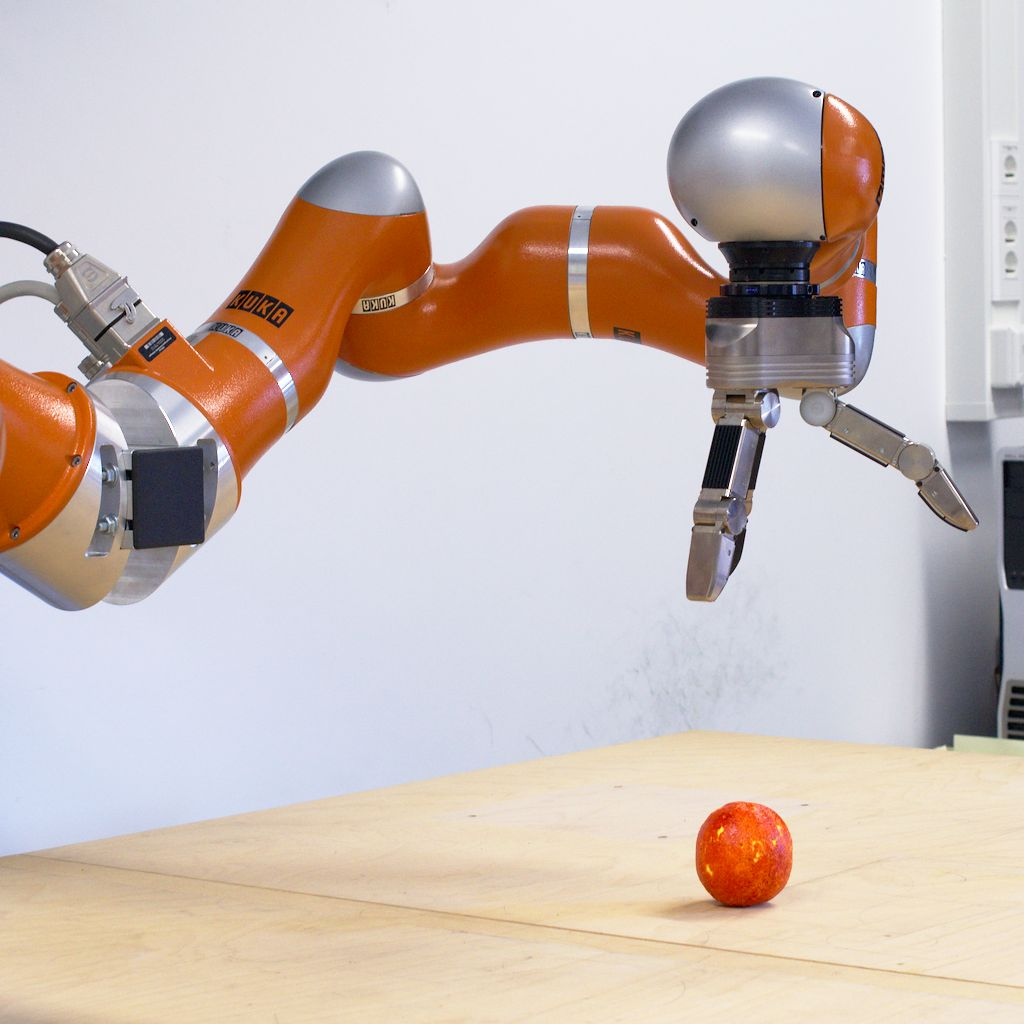
\includegraphics[width=0.5\textwidth]{./figures/sec/kuka.jpg}
  \caption{One of the two Kuka Lightweight Robots~\cite{bischoff2010kukadlr}. Connected to the robot arm is a three-fingered gripper.}
  \label{fig:sec_introduction_kuka}
\end{figure}

In recent years, developments in the field of robotics have emerged solutions to a very wide field of problems: Ranging from autonomous driving to search and rescue missions in remote areas; from space exploration tasks to the care of elderly people.
This also means that robots become more and more integrated into our daily life.
Along come increasingly complex situations, which need to be mastered.
Planning plays a vital part here.

Historically, planning in robotics is divided into two fields: on the one side there are voltages and currents to be controlled.
In this domain physical constraints are most important, \ie robot hardware, collision detection, collision avoidance, and a dynamically feasible trajectory~\cite{choset2005, plaku2010}.
On the other side there are higher level descriptors, which work in the symbolic domain.
One example for two symbols might be \emph{empty cup} and \emph{cup full of water}.
Now, a transfer function \emph{fill cup with water} to arrive at the second symbol from the first can be defined.
Furthermore, the fact that the cup must be empty in order to fill it with water is called precondition.
Preconditions ensure that only transfer functions are applied to symbols, where it makes sense.
For example, filling a full cup with more water would result in spilling.
Similarly, the filled cup is called postcondition of the filling action~\cite[p. 66f., p. 335f.]{golding2006interactive}.
The transition from raw sensor data to a symbolic descriptor is again the above mentioned signal-to-symbol gap and both planning approaches are separated by this gap.
They are considered as two different problems~\cite{arkin1990, payton1990, belta2007}, where the first one is bottom-up and the second one top-down.
In this work, the gap is bridged using a bottom-up method, which requires almost no higher level knowledge.
This is one of the biggest advantages compared to current state-of-the-art.

One of the main obstacles in this field of robotic science is acquiring these symbolic descriptors from sensor data.
This poses a critical problem in two respects.
First, it is needed for logic-based reasoning and the resulting descriptors form the basis for further learning.
Second, it is essential for higher-level planning.
The planning component uses the resulting descriptors instead of sensor data.
There are numerous ways of bridging the signal-to-symbol gap.
First, one needs to define how a logical sequence of sensor signals can be divided into actions and subactions, where each part may be connected to a logical symbol.
Second, this must happen in an automatic manner.

Planning and learning usually happens in the symbolic domain.
A discrete state space, including discrete actions, is assumed.
Throughout the years, a lot of progress has been achieved and various complex domain description languages, such as STRIPS~\cite{fikes1971}, PDDL~\cite{mcdermott1998}, HAL~\cite{marthi2007}, or ADL~\cite{pednault1994}, have been developed to meet the increasingly demanding \gls{ac:ai} tasks.
Various approaches exist to solve discrete problems in the defined domain~\cite{kuter2009} and even high level frameworks exist for easy implementation~\cite{agostinitorraswoergoetter2017, de2009indigolog}.

Thus, more elaborate decision making systems have been proposed to integrate the motion planning more tightly into the action planning domain.
In~\cite{hauser2009, kaelbling2011, plaku2010} a forward-search planner is used.
The task plan is built and the feasibility is continuously checked by a geometric/low level motion planner and being replanned in cases of error.
With this motivation in~\cite{caldiran2009, eyerich2010}, an interface is introduced, which provides ``external predicates''.
These functions are used in the action domain description for checking the feasibility of a primitive action by a motion planner~\cite{erdem2011}.
In~\cite{eyerich2010} the planning language PDDL~\cite{mcdermott1998} is extended with so called semantic attachments and the motion planner is changed accordingly.

It has been shown that there is a fine line when taking low level information, \ie geometric features into account~\cite{erdem2011}.
Obviously, some information is needed for action execution and while a task often can be solved this way, the resulting plan might be inefficient or unfeasible.
Taking some high level information into account, a plan made up from low level information can often be enhanced~\cite{erdem2011}.
In this work, a novel approach to planning on a very low abstraction level is introduced: First, it is shown that even without high level knowledge a very wide variety of tasks on that level can be solved.
Second, this low level of abstraction can be utilized to retrieve a motor signal in a straightforward way, but also can access the higher level symbolic domain easily.
This means, this planner can be used as a way to bridge the signal-to-symbol gap.
Therefore, a third abstraction layer between the motion planner and a high level symbolic planner is employed and thus combines the advantages of low- and high level planning.
Again, actions are represented by Semantic Event Chains.
In this work, it is shown that using \glspl{ac:sec} and further enriching those by pre- and postconditions, an already very powerful action decision framework is built.
This way the framework does not depend on high level symbolic knowledge, but is rather built using a bottom-up method.

\section{Methods}
\label{sec:action_methods}

\begin{figure}[]
  \centering
  % Define block styles
\tikzstyle{block} = [draw, rectangle, fill=white, minimum height=3.5cm, minimum width=6.0cm, text width=4.5cm, text centered, rounded corners=true]
\tikzstyle{blockBox} = [draw, inner sep=0.2cm, dashed, rectangle, minimum width=3.5cm, text centered, rounded corners=true]
\tikzstyle{blockText} = [text centered, minimum height=1.5cm,text width=5.0cm]
\tikzstyle{arrow} = [draw, -latex]

\definecolor{red1}{RGB}{160,0,0}
\definecolor{green1}{RGB}{0,160,0}
\definecolor{blue1}{RGB}{0,0,160}

% Define images
\pgfdeclareimage[height=3.0cm]{scene}{./figures/sensor/methods_flowchart_scene.jpg}
\pgfdeclareimage[height=3.0cm]{robot}{./figures/sensor/methods_flowchart_robot.jpg}
	      
\begin{tikzpicture}[node distance = 8.0cm, auto]
  % Scene
  \node[block] (scene) {\pgfuseimage{scene}};

  % Hardware setup
  \node [block, right of=scene] (hardwaresetup) {\pgfuseimage{robot}};

	% Filter
  \node [block, below of=scene, node distance=6.5cm] (filter) {Removing noise and outliers};
  
  % VO
  \node [block, right of=filter] (vo) {Estimating pose, position, and environment};
  

  % Text
  \node [blockText, above of=scene, node distance=2.5cm] (scene_t) {\textbf{a) Scene}};
  \node [blockText, above of=hardwaresetup, node distance=2.5cm] (hardwaresetup_t) {\textbf{b) Hardware setup}\\\secref{ssec:perception_methods_hardwaresetup}};
  \node [blockText, above of=filter, node distance=2.5cm] (filter_t) {\textbf{c) Preprocessing}\\\secref{ssec:perception_methods_noiseandoutlierdetection}};
  \node [blockText, above of=vo, node distance=2.5cm] (vo_t) {\textbf{d) Visual Odometry}\\\secref{ssec:perception_methods_visualodometryalgorithm}};


  % Fit
  \node[fit=(scene)(scene_t), blockBox] (scene_f) {};
  \node[fit=(hardwaresetup)(hardwaresetup_t), blockBox] (hardwaresetup_f) {};
  \node[fit=(filter)(filter_t), blockBox] (filter_f) {};
  \node[fit=(vo)(vo_t), blockBox] (vo_f) {};


  % Arrows
	\path [arrow] (scene_f.east) to (hardwaresetup_f.west);
	\path [arrow] (hardwaresetup_f.south) -| ++(0,-0.55cm) -| (filter_f.north);
	\path [arrow] (filter_f.east) to (vo_f.west);
\end{tikzpicture}

  \caption{Flowchart of the methods in this chapter and how they relate. Details are explained in \secref{sec:action_methods}.}
  \label{fig:actions_methods_flowchart}
\end{figure}

In this section, approaches to planning are introduced.
An overview is given in \figref{fig:actions_methods_flowchart}: First, a) the scene is recorded as RGB-D image by an Asus Xtion Pro camera and a Nikon high resolution \gls{ac:dslr}.
Each depth frame is b) preprocessed by computer vision algorithms.
They are segmented via the Locally Convex Connected Patches (LCCP) algorithm~\cite{stein2014object} into clusters, where each cluster correlates to one object candidate.
For object recognition~\cite{schoeler2014fast} is used; objects are tracked via~\cite{paponkulviciusaksoy2013}. 
All parts of the algorithms are integrated as modular \gls{ac:ros} nodes~\cite{quigleyconleygerkey2009}.
Next, the objects are categorized based on c) an action ontology, \secref{ssec:action_methods_actioncategories}.
This categorization is used throughout the rest of this thesis.
Based on this information, a graph structure is retrieved in d) \acrlong{ac:sec} (\secref{ssec:action_methods_semanticeventchains}).
As first contribution, the graph is enriched with pose information by e) a novel 3d reasoning algorithm (\secref{ssec:action_methods_enrichedsemanticeventchains}).
Afterwards, it is shown in f) that each graph can be reduced to only three different subgraphs (\secref{ssec:action_methods_structuralinformation}).
This in turn is used to compute g) a scene's affordance (\secref{ssec:action_methods_affordanceofsemanticeventchains}).
Here, for example the question is asked: ``Given a tomato, a knife, and a cutting board, what can one do with these objects?''
In h), it is shown how the approach can be extended for complex action planning (\secref{ssec:action_methods_usingaffordanceforplanning}).
As an example it is analyzed what actions a robot needs to perform when given the command ``Make me a sandwich.''

\subsection{Action categories}
\label{ssec:action_methods_actioncategories}

In this section, we will first define the action domain.
Here, the focus lies on actions involving hands and objects (and thus not gestures, \etc).
Reasoning about actions seemed for a long time of purely philosophical interest and a detailed review can be found in~\cite{aune1977reason}.
The same author states the major viewpoints~\cite{worgotter2013simple} on action ontologies as:~\cite[p. 195]{aune1988action}

\begin{quote}
``Perhaps the most controversial aspect of so called action theory is its subject matter.
This subject matter is generally said to be (or to concern) actions, but different philosophers conceive of actions in radically different ways. 
For some philosophers actions are abstract entities – states of affairs, propositions, sets, or even ordered pairs of some kind. 
For others, actions are distinctively concrete entities located in space and time. 
Another group of philosophers, among whom I include myself, have even denied that actions are required for a reasonable action theory, insisting that agents or actors will suffice as the theory's sole objects.''
\end{quote}

However, apart from the entity concept of an action, one needs to ask the question: ``What is an object?''
Originally, this subject was perceived as bottom-up and being object-driven.
This means different objects allow for different actions.
This is the so-called affordance principle~\cite{shaw2017perceiving}.

As stated in~\cite{worgotter2013simple} agency on the other hand suggests that the intended action lets the agent seek for appropriate objects.
This point of view leads away from the question ``What can you do with all the things in the world'', but rather points to the question of ``What can you do with your hands?'' and recent concepts suggest that objects and actions are intertwined~\cite{turchin1993cybernetic}.
In~\textcite{worgotter2013simple} it is shown that based on touching relations one can separate actions naturally.
This concept is introduced in the following sections in more detail.

Also stemming from this concept in~\cite{worgotter2013simple} an action ontology is derived, which assumes 26 atomic one-handed actions as shown in \tabref{tab:sec_definitionofactions_actiontable}.
Every sequence of actions, \eg ``make a sandwich'', can be broken down into a sequence of atomic actions:

\begin{table}[]
\resizebox{\textwidth}{!}{%
  \centering
  \begin{tabular}{cccll}
    \toprule
    Nr  & Type  & Goal  & Instantiation & Example\\
    \midrule
    1   & 1 & r     & Punch/hit         & with your hand an object\\
    2   & 1 & r     & Flick             & with your finger nail, quickly\\
    3   & 1 & r     & Poke              & with your finger tip, slowly\\
    4   & 1 & d     & Chop              & quickly, with the edge of your hand\\
    5   & 1 & r     & Turn = bore (rotate wrist x) & a hole with your finger or your hand\\
    6   & 1 & d     & Cut               & slowly, with the edge of your hand\\
    7   & 1 & d/r   & Scratch           & with your finger nail\\
    8   & 1 & d     & Scissor-cut/pinch & between your fingers\\
    9   & 1 & d/r   & Squash, squeeze   & inside your fist\\
    10  & 1 & d     & Draw              & with finger in sand\\
    11  & 1 & r     & Push/pull-without-grasp & regular push, hook-pull, adduct with finger\\
    12  & 1 & r     & Stir              & with finger\\
    13  & 1 & r     & Knead             & kneading dough, \etc\\
    14  & 1 & r     & Rub/massage       & with your hand someone else's body\\
    15  & 1 & r     & Lever (rotate wrist y)    & \eg break open a hole\\
    16  & 1 & d     & Scoop/ladle       & fill your hand with liquid\\
    \midrule
    17  & 2 & t     & Take Down or Pick apart   & one block from a laterally connected\\
        &   &       &                           & group or a pile by pick \& place\\
    18  & 2 & t     & Push down or push apart   & one block from a laterally connected\\
        &   &       &                           & group or a pile by pushing\\
    19  & 2 & b     & Rip off           & Rip a piece off an object\\
    20  & 2 & b     & Break off         & Break a piece off an object\\
    21  & 2 & b     & Uncover by pick \& place    & Pick off an object to uncover another\\
        &   &       &                           & object\\
    22  & 2 & b     & Uncover by pushing        & Push off an object to uncover another\\
        &   &       &                           & object\\
    \midrule
    23  & 3 & c     & Put on top or Put together    & two blocks on top of each other or side\\
        &   &       &                               & by side by pick \& place\\
    24  & 3 & c     & Push on top or push together  & two blocks on top of each other or side\\
        &   &       &                               & by side by pushing\\
    25  & 3 & h     & Put over          & Put one object above another one to\\
        &   &       &                   & cover it completely\\
    26  & 3 & h     & Push over         & Push one object above another one to\\
        &   &       &                   & cover it completely\\
    \bottomrule
  \end{tabular}
}
  \caption{List of atomic actions as taken from~\cite{worgotter2013simple}. 
      More actions are listed as ``Some (sic) dynamic versions of 17 -- 26''; for example, the action ``throw-in''.
      According to~\cite{worgotter2013simple} there are three different manipulation types (listed in the ``Type'' column): 1: Hand-only-actions; 2: Separation actions; 3: Release determined actions.
      Abbreviations in the ``Goal'' column are defined as follows: d: destroying; r: rearranging; c: constructing; t: taking-down; h: hiding; and b: breaking.}
  \label{tab:sec_definitionofactions_actiontable}
\end{table}

\begin{enumerate}
  \item \action{Pick \& Place} the bread from the table on the cutting board,
  \item \action{Cut} the bread,
  \item \action{Scoop} marmelade,
  \item \action{Put} marmelade \action{on top} of the bread.
\end{enumerate}

Each action is categorized into three types and each type into two goal categories:

\begin{enumerate}
  \item Hand-only actions:
    \begin{itemize}
      \item Rearrange (\eg hit, push, stir),
      \item Destroy (\eg cut, draw, scoop),
    \end{itemize}
  \item Separation actions:
    \begin{itemize}
      \item Take-down (\eg take-down, push apart)
      \item Break (\eg rip off, uncover by pick \& place),
    \end{itemize}
  \item Release determined actions:
    \begin{itemize}
      \item Construct (\eg put on top, push together),
      \item Hide (\eg. put over, push over),
    \end{itemize}
\end{enumerate}

where actions from each goal category share similar trajectories.
Next, one needs to define object roles.
These roles are determined by the changes that occur following an action in the relation of an object to other objects. 
An action involves at least two objects: a \emph{hand} and a \emph{main} object. 
The resulting object list (\emph{hand}, \emph{main}, \emph{primary}, \emph{secondary}, \etc) and their abstract roles are as followed (taken from~\textcite{reichaeinwoergoetter2018}):

\begin{itemize}
  \item \emph{Hand} (The object that performs the action): not touching anything at the beginning and the end of the action. It touch\-es at least one object during the manipulation.
  \item \emph{Main} (The object which is directly in contact with the hand): not touching the hand at the beginning and the end of action. It touches the hand at least once during the manipulation.
  \item \emph{Primary} (The object from which the \emph{main} object separates): initially touches the \emph{main} object. Changes its relation to not-touching during the action.
  \item \emph{Secondary} (The object to which the \emph{main} object joins): initially does not touch the \emph{main} object. Changes its relation to touching during the action.
  \item \emph{Load} (The object which is indirectly manipulated): does not touch the hand. This object touches/ untouches the \emph{main} and untouches/ touches the \emph{container} during the action .
  \item \emph{Container} (The object whose relation with \emph{load} changes and which is not the \emph{main} object): touches or untouches the \emph{load} object.
  \item \emph{Main support} (The object on which the \emph{main} object is located): touching the \emph{main} object at least once.
  \item \emph{Primary support} (The object on which the \emph{primary} object is located): touching the \emph{primary} object at least once.
  \item \emph{Secondary support} (The object on which the \emph{secondary} is located): touching the \emph{secondary} object at least once.
  \item \emph{Tool} (The object which is used by the hand to enhance the quality of some actions): touching the hand all the time.
\end{itemize}

When looking at object roles a different categorization of actions comes to mind: One can define action categories based upon the objects, which the hand interacts with.
These fall into three classes:

\begin{enumerate}
  \item Actions with \emph{main support}: In this category the \emph{main} object is always in touch with the \emph{main support}; an example is shown in \figref{fig:sec_definitionofactions_actionscategory_1}.
  \item Actions without \emph{main support}: In this category the \emph{main} object is lifted from the \emph{primary} object; an example is shown in \figref{fig:sec_definitionofactions_actionscategory_2}.
  \item Actions with \emph{load} and \emph{container}: In this category a \emph{container} with \emph{load}, \eg a glass filled with water, is used; an example is shown in \figref{fig:sec_definitionofactions_actionscategory_3}.
\end{enumerate}

A detailed list of actions is shown in \tabref{tab:sec_definitionofactions_ontologysummary}.
While the first categorization places its focus on the high level goal of the action, the second one is derived from the bottom-up point of view of an object's structural role.
In the following sections we will see that the structural role is also important for affordance and planning.

\begin{table}[]
  \begin{tabular}{p{3cm} p{6cm} p{3cm}}
    \toprule
    \multirow{2}{*}{Category}   & \multirow{2}{*}{Sub-Category} & Example\\
                                &                               & Actions\\
    \midrule
    \multirow{4}{3.0cm}{\vspace{1.5cm} \textcolor{white}{~~~~~~~~~~~~~~~~~} Actions with main support} & Actions with hand, main, and main support      & push, punch, flick\\ \cmidrule(l){2-3}
                & Actions with hand, main, main support, and primary                 & push apart, cut, chop\\ \cmidrule(l){2-3}
                & Actions with hand, main, main support, and secondary               & push together\\ \cmidrule(l){2-3}
                & Actions with hand, main, main support, primary, and secondary      & push from a to b\\
    \midrule
    \multirow{5}{3.0cm}{\vspace{1.5cm} \textcolor{white}{~~~~~~~~~~~~~~~~~} Actions without main support (These action have primary, secondary and their supports)}  & primary $\ne$ secondary and primary support $\ne$ secondary support  & pick and place, break off\\ \cmidrule(l){2-3}\
                & primary $\ne$ secondary and primary support $=$ secondary support & pick and place, break off\\ \cmidrule(l){2-3}
                & primary $\ne$ secondary and primary $=$ secondary support         & put on top\\ \cmidrule(l){2-3}
                & primary $\ne$ secondary and primary support $=$ secondary         & pick apart\\ \cmidrule(l){2-3}
                & primary $=$ secondary                                             & pick and place, break off \\
    \midrule
    \multirow{2}{3.0cm}{\vspace{-0.25cm} \textcolor{white}{~~~~~~~~~~~~~~~~~} Actions with load and~container} & The relation of load and main changes from N to T (loading)    & Pipetting\\ \cmidrule(l){2-3}
                & The relation of load and main changes from T to N  (unloading)    & Pour, Drop\\
    \bottomrule
  \end{tabular}
  \caption{Summary of ontology of actions. Actions are divided into three categories and further into sub-categories. There can be more than one action in each sub-category. Taken from~\textcite{reichaeinwoergoetter2018}.}
  \label{tab:sec_definitionofactions_ontologysummary}
\end{table}

\begin{figure}[]
  \begin{subfigure}[]{\textwidth}
    \centering
    % Define block styles
\tikzstyle{block} = [rectangle, fill=white, text width=1em, text centered, minimum height=0.5em, rounded corners=true]
\tikzstyle{blockBox} = [draw, rectangle, fill=white, minimum height=2.5cm, minimum width=4.5cm, text width=1em, text centered, rounded corners=true]

\tikzstyle{blockSupP} = [draw, rectangle, fill=red1!20, minimum height=0.6cm, minimum width=1.3cm, text width=1em, text centered, rounded corners=true]
\tikzstyle{blockSupM} = [draw, rectangle, fill=green1!20, minimum height=0.6cm, minimum width=1.3cm, text width=1em, text centered, rounded corners=true]
\tikzstyle{blockSupS} = [draw, rectangle, fill=blue1!20, minimum height=0.6cm, minimum width=1.3cm, text width=1em, text centered, rounded corners=true]
\tikzstyle{blockSup} = [draw, rectangle, fill=red1!20, minimum height=0.6cm, minimum width=3.5cm, text width=3.5cm, text centered, rounded corners=true]

\tikzstyle{blockCon} = [draw, rectangle, fill=white, minimum height=0.5cm, minimum width=1cm, text width=0.6cm, text centered, rounded corners=true]
\tikzstyle{blockP} = [draw, rectangle, fill=red1!40, minimum height=0.6cm, minimum width=0.6cm, text width=1em, text centered, rounded corners=true]
\tikzstyle{blockM} = [draw, rectangle, fill=green1!40, minimum height=0.6cm, minimum width=0.6cm, text width=1em, text centered, rounded corners=true]
\tikzstyle{blockS} = [draw, rectangle, fill=blue1!40, minimum height=0.6cm, minimum width=0.6cm, text width=1em, text centered, rounded corners=true]
\tikzstyle{blockL} = [draw, rectangle, fill=black!20, minimum height=0.6cm, minimum width=0.6cm, text width=1em, text centered, rounded corners=true]
\tikzstyle{arrow} = [draw, -latex]

\definecolor{red1}{RGB}{160,0,0}
\definecolor{green1}{RGB}{0,160,0}
\definecolor{blue1}{RGB}{0,0,160}

\pgfdeclareimage[width=0.6cm]{hand}{./figures/sec/robothand.jpg}

	      
\begin{tikzpicture}[node distance=6em, auto]
	%%%%%%%%%%%%%%%%%%%%%%%%%%%%%%%%%%%%%%%%%%%%%%%%%%%%%%%%%%%%%%%%%%%%%%%%%%%%%%%%%%%%%%%%%%%%%%%%%%%%%%
	% First line
	\node [blockBox] (p11) {};
	\node [blockBox, right of=p11, node distance=5cm] (p12) {};
	\node [blockBox, below of=p11, node distance=3.0cm] (p13) {};
	\node [blockBox, right of=p13, node distance=5cm] (p14) {};
	\node [blockBox, below of=p13, node distance=3.0cm] (p15) {};

	% Panel number
	\node[below left] at (p11.north east) {1};
	\node[below left] at (p12.north east) {2};
	\node[below left] at (p13.north east) {3};
	\node[below left] at (p14.north east) {4};
	\node[below left] at (p15.north east) {5};

	% Panel 11
	\node [above right, xshift=0.3cm, blockSup, minimum width=3cm] at (p11.south west) (p11_Sup) {\small{p.s~=~m.s~=~s.s}};

	\node [above of=p11_Sup, blockP, node distance=0.6cm, xshift=-1.2cm] (p11_p) {\small{p}};
	\node [above of=p11_Sup, blockM, node distance=0.6cm, xshift=-0.5cm] (p11_m) {\small{m}};
	\node [above of=p11_Sup, blockS, node distance=0.6cm, xshift= 1.2cm] (p11_s) {\small{s}};

	\node [above of=p11_p, node distance=1.1cm, xshift=1.4cm] (p11_h) {\pgfuseimage{hand}};

	% Panel 12
	\node [above right, xshift=0.3cm, blockSup, minimum width=3cm] at (p12.south west) (p12_Sup) {\small{p.s~=~m.s~=~s.s}};

	\node [above of=p12_Sup, blockP, node distance=0.6cm, xshift=-1.2cm] (p12_p) {\small{p}};
	\node [above of=p12_Sup, blockM, node distance=0.6cm, xshift=-0.5cm] (p12_m) {\small{m}};
	\node [above of=p12_Sup, blockS, node distance=0.6cm, xshift= 1.2cm] (p12_s) {\small{s}};

	\node [above of=p12_m, node distance=0.6cm, xshift=-0.2cm] (p12_h) {\pgfuseimage{hand}};
	\node [above of=p12_Sup, blockP, node distance=0.6cm, xshift=-1.2cm] (p12_p) {\small{p}};
	\node [above of=p12_Sup, blockM, node distance=0.6cm, xshift=-0.5cm] (p12_m) {\small{m}};

	% Panel 13
	\node [above right, xshift=0.3cm, blockSup, minimum width=3cm] at (p13.south west) (p13_Sup) {\small{p.s~=~m.s~=~s.s}};

	\node [above of=p13_Sup, blockP, node distance=0.6cm, xshift=-1.2cm] (p13_p) {\small{p}};
	\node [above of=p13_Sup, blockM, node distance=0.6cm, xshift= 0.0cm] (p13_m) {\small{m}};
	\node [above of=p13_Sup, blockS, node distance=0.6cm, xshift= 1.2cm] (p13_s) {\small{s}};

	\node [above of=p13_m, node distance=0.6cm, xshift=-0.2cm] (p13_h) {\pgfuseimage{hand}};
	\node [above of=p13_Sup, blockM, node distance=0.6cm, xshift= 0.0cm] (p13_m) {\small{m}};

	% Panel 14
	\node [above right, xshift=0.3cm, blockSup, minimum width=3cm] at (p14.south west) (p14_Sup) {\small{p.s~=~m.s~=~s.s}};

	\node [above of=p14_Sup, blockP, node distance=0.6cm, xshift=-1.2cm] (p14_p) {\small{p}};
	\node [above of=p14_Sup, blockM, node distance=0.6cm, xshift= 0.5cm] (p14_m) {\small{m}};
	\node [above of=p14_Sup, blockS, node distance=0.6cm, xshift= 1.2cm] (p14_s) {\small{s}};

	\node [above of=p14_m, node distance = 0.58cm, xshift=-0.2cm] (p14_h) {\pgfuseimage{hand}};
	\node [above of=p14_Sup, blockM, node distance=0.6cm, xshift= 0.5cm] (p14_m) {\small{m}};

	% Panel 15
	\node [above right, xshift=0.3cm, blockSup, minimum width=3cm] at (p15.south west) (p15_Sup) {\small{p.s~=~m.s~=~s.s}};

	\node [above of=p15_Sup, blockP, node distance=0.6cm, xshift=-1.2cm] (p15_p) {\small{p}};
	\node [above of=p15_Sup, blockM, node distance=0.6cm, xshift= 0.5cm] (p15_m) {\small{m}};
	\node [above of=p15_Sup, blockS, node distance=0.6cm, xshift= 1.2cm] (p15_s) {\small{s}};

	\node [above of=p15_m, node distance = 1cm] (p15_h) {\pgfuseimage{hand}};
\end{tikzpicture}

    \caption{Example action with \emph{main support}: \action{Pushing}.}
    \label{fig:sec_definitionofactions_actionscategory_1}
  \end{subfigure}
  \begin{subfigure}[]{\textwidth}
    \centering
    % Define block styles
\tikzstyle{block} = [rectangle, fill=white, text width=1em, text centered, minimum height=0.5em, rounded corners=true]
\tikzstyle{blockBox} = [draw, rectangle, fill=white, minimum height=2.5cm, minimum width=4.5cm, text width=1em, text centered, rounded corners=true]

\tikzstyle{blockSupP} = [draw, rectangle, fill=red1!20, minimum height=0.6cm, minimum width=1.3cm, text width=1em, text centered, rounded corners=true]
\tikzstyle{blockSupM} = [draw, rectangle, fill=green1!20, minimum height=0.6cm, minimum width=1.3cm, text width=1em, text centered, rounded corners=true]
\tikzstyle{blockSupS} = [draw, rectangle, fill=blue1!20, minimum height=0.6cm, minimum width=1.3cm, text width=1em, text centered, rounded corners=true]
\tikzstyle{blockSup} = [draw, rectangle, fill=red1!20, minimum height=0.6cm, minimum width=3.5cm, text width=3.5cm, text centered, rounded corners=true]

\tikzstyle{blockCon} = [draw, rectangle, fill=white, minimum height=0.6cm, minimum width=1cm, text width=0.6cm, text centered, rounded corners=true]
\tikzstyle{blockP} = [draw, rectangle, fill=red1!40, minimum height=0.6cm, minimum width=0.6cm, text width=1em, text centered, rounded corners=true]
\tikzstyle{blockM} = [draw, rectangle, fill=green1!40, minimum height=0.6cm, minimum width=0.6cm, text width=1em, text centered, rounded corners=true]
\tikzstyle{blockS} = [draw, rectangle, fill=blue1!40, minimum height=0.6cm, minimum width=0.6cm, text width=1em, text centered, rounded corners=true]
\tikzstyle{blockL} = [draw, rectangle, fill=black!20, minimum height=0.6cm, minimum width=0.6cm, text width=1em, text centered, rounded corners=true]
\tikzstyle{arrow} = [draw, -latex]

\definecolor{red1}{RGB}{160,0,0}
\definecolor{green1}{RGB}{0,160,0}
\definecolor{blue1}{RGB}{0,0,160}

\pgfdeclareimage[width=0.6cm]{hand}{./figures/sec/robothand.jpg}

	      
\begin{tikzpicture}[node distance=6em, auto]
	%%%%%%%%%%%%%%%%%%%%%%%%%%%%%%%%%%%%%%%%%%%%%%%%%%%%%%%%%%%%%%%%%%%%%%%%%%%%%%%%%%%%%%%%%%%%%%%%%%%%%%
	% second line
	\node [blockBox] (p21) {};
	\node [blockBox, right of=p21, node distance=5cm] (p22) {};
	\node [blockBox, below of=p21, node distance=3cm] (p23) {};
	\node [blockBox, right of=p23, node distance=5cm] (p24) {};
	\node [blockBox, below of=p23, node distance=3cm] (p25) {};

	% panel number
	\node[below left] at (p21.north east) {1};
	\node[below left] at (p22.north east) {2};
	\node[below left] at (p23.north east) {3};
	\node[below left] at (p24.north east) {4};
	\node[below left] at (p25.north east) {5};

	% Panel 21

	\node [above right, xshift=0.3cm, blockSupP] at (p21.south west) (p21_ps) {\small{p.s}};
	\node [right of=p21_ps, blockSupS, node distance=2.5cm] (p21_ss) {\small{s.s}};

	\node [above of=p21_ps, blockP, node distance=0.6cm] (p21_p) {\small{p}};
	\node [above of=p21_p, blockM, node distance=0.6cm] (p21_m) {\small{m}};
	\node [above of=p21_ss, blockS, node distance=0.6cm] (p21_s) {\small{s}};

	\node [above of=p21_m, node distance = 0.0cm, xshift=1cm] (p21_h) {\pgfuseimage{hand}};

	% Panel 22
	\node [above right, xshift=0.3cm, blockSupP] at (p22.south west) (p22_ps) {\small{p.s}};
	\node [right of=p22_ps, blockSupS, node distance=2.5cm] (p22_ss) {\small{s.s}};

	\node [above of=p22_ps, blockP, node distance=0.6cm] (p22_p) {\small{p}};
	\node [above of=p22_p, blockM, node distance=0.6cm] (p22_m) {\small{m}};
	\node [above of=p22_ss, blockS, node distance=0.6cm] (p22_s) {\small{s}};

	\node [above of=p22_m, node distance = 0.45cm, xshift=-0.3cm] (p22_h) {\pgfuseimage{hand}};
	\node [above of=p22_p, blockM, node distance=0.6cm] (p22_m) {\small{m}};

	% Panel 23
	\node [above right, xshift=0.3cm, blockSupP] at (p23.south west) (p23_ps) {\small{p.s}};
	\node [right of=p23_ps, blockSupS, node distance=2.5cm] (p23_ss) {\small{s.s}};

	\node [above of=p23_ps, blockP, node distance=0.6cm] (p23_p) {\small{p}};
	\node [above of=p23_p, blockM, node distance=0.62cm, xshift=1cm] (p23_m) {\small{m}};
	\node [above of=p23_ss, blockS, node distance=0.6cm] (p23_s) {\small{s}};

	\node [above of=p23_m, node distance = 0.45cm, xshift=-0.3cm] (p23_h) {\pgfuseimage{hand}};
	\node [above of=p23_p, blockM, node distance=0.62cm, xshift=1cm] (p23_m) {\small{m}};

	% Panel 24
	\node [above right, xshift=0.3cm, blockSupP] at (p24.south west) (p24_ps) {\small{p.s}};
	\node [right of=p24_ps, blockSupS, node distance=2.5cm] (p24_ss) {\small{s.s}};

	\node [above of=p24_ps, blockP, node distance=0.6cm] (p24_p) {\small{p}};
	\node [above of=p24_ss, blockS, node distance=0.6cm] (p24_s) {\small{s}};
	\node [above of=p24_s, blockM, node distance=0.6cm] (p24_m) {\small{m}};

	\node [above of=p24_m, node distance = 0.45cm, xshift=-0.3cm] (p24_h) {\pgfuseimage{hand}};
	\node [above of=p24_s, blockM, node distance=0.6cm] (p24_m) {\small{m}};

	% Panel 25
	\node [above right, xshift=0.3cm, blockSupP] at (p25.south west) (p25_ps) {\small{p.s}};
	\node [right of=p25_ps, blockSupS, node distance=2.5cm] (p25_ss) {\small{s.s}};

	\node [above of=p25_ps, blockP, node distance=0.6cm] (p25_p) {\small{p}};
	\node [above of=p25_ss, blockS, node distance=0.6cm] (p25_s) {\small{s}};
	\node [above of=p25_s, blockM, node distance=0.6cm] (p25_m) {\small{m}};

	\node [above of=p25_m, node distance = 0.55cm, xshift=-1.0cm] (p25_h) {\pgfuseimage{hand}};
\end{tikzpicture}

    \caption{Example action without \emph{main support}: \action{Pick and place}.}
    \label{fig:sec_definitionofactions_actionscategory_2}
  \end{subfigure}
\end{figure}
\begin{figure}[]\ContinuedFloat
  \begin{subfigure}[]{\textwidth}
    \centering
    % Define block styles
\tikzstyle{block} = [rectangle, fill=white, text width=1em, text centered, minimum height=0.5em, rounded corners=true]
\tikzstyle{blockBox} = [draw, rectangle, fill=white, minimum height=3cm, minimum width=5.5cm, text width=1em, text centered, rounded corners=true]

\tikzstyle{blockSupP} = [draw, rectangle, fill=red1!20, minimum height=0.6cm, minimum width=1.3cm, text width=1em, text centered, rounded corners=true]
\tikzstyle{blockSupM} = [draw, rectangle, fill=green1!20, minimum height=0.6cm, minimum width=1.3cm, text width=1em, text centered, rounded corners=true]
\tikzstyle{blockSupS} = [draw, rectangle, fill=blue1!20, minimum height=0.6cm, minimum width=1.3cm, text width=1em, text centered, rounded corners=true]
\tikzstyle{blockSup} = [draw, rectangle, fill=red1!20, minimum height=0.6cm, minimum width=3.5cm, text width=3.5cm, text centered, rounded corners=true]

\tikzstyle{blockCon} = [draw, rectangle, fill=white, minimum height=0.6cm, minimum width=1.3cm, text width=1.2cm, text centered, rounded corners=true]
\tikzstyle{blockP} = [draw, rectangle, fill=red1!40, minimum height=0.6cm, minimum width=0.6cm, text width=1em, text centered, rounded corners=true]
\tikzstyle{blockM} = [draw, rectangle, fill=green1!40, minimum height=0.6cm, minimum width=0.6cm, text width=1em, text centered, rounded corners=true]
\tikzstyle{blockS} = [draw, rectangle, fill=blue1!40, minimum height=0.6cm, minimum width=0.6cm, text width=1em, text centered, rounded corners=true]
\tikzstyle{blockL} = [draw, rectangle, fill=black!20, minimum height=0.6cm, minimum width=0.6cm, text width=1em, text centered, rounded corners=true]
\tikzstyle{arrow} = [draw, -latex]

\definecolor{red1}{RGB}{160,0,0}
\definecolor{green1}{RGB}{0,160,0}
\definecolor{blue1}{RGB}{0,0,160}

\pgfdeclareimage[width=0.6cm]{hand}{./figures/sec/robothand.jpg}

	      
\begin{tikzpicture}[node distance=6em, auto]
	%%%%%%%%%%%%%%%%%%%%%%%%%%%%%%%%%%%%%%%%%%%%%%%%%%%%%%%%%%%%%%%%%%%%%%%%%%%%%%%%%%%%%%%%%%%%%%%%%%%%%%
	% third line
	\node [blockBox] (p31) {};
	\node [blockBox, right of=p31, node distance=6cm] (p32) {};
	\node [blockBox, below of=p31, node distance=3.5cm] (p33) {};
	\node [blockBox, right of=p33, node distance=6cm] (p34) {};
	\node [blockBox, below of=p33, node distance=3.5cm] (p35) {};

	\node [blockBox, right of=p35, node distance=6cm] (p36) {};
	\node [blockBox, below of=p35, node distance=3.5cm] (p37) {};

	% panel number
	\node[below left] at (p31.north east) {1};
	\node[below left] at (p32.north east) {2};
	\node[below left] at (p33.north east) {3};
	\node[below left] at (p34.north east) {4};
	\node[below left] at (p35.north east) {5};
	\node[below left] at (p36.north east) {6};
	\node[below left] at (p37.north east) {7};

	% Panel 31
	\node [above right, xshift=0.4cm, blockSupP] at (p31.south west) (p31_ps) {\small{p.s}};
	\node [right of=p31_ps, blockSupS, node distance=1.7cm] (p31_ss) {\small{s.s}};
	\node [right of=p31_ss, blockCon, node distance=1.7cm] (p31_con) {\small{cont}};

	\node [above of=p31_ps, blockP, node distance=0.6cm] (p31_p) {\small{p}};
	\node [above of=p31_p, blockM, node distance=0.6cm] (p31_m) {\small{m}};
	\node [above of=p31_m, blockL, node distance=0.6cm] (p31_l) {\small{l}};
	\node [above of=p31_ss, blockS, node distance=0.6cm] (p31_s) {\small{s}};

	\node [above of=p31_m, node distance = 0.15cm, xshift=2.5cm] (p31_h) {\pgfuseimage{hand}};

	% Panel 32
	\node [above right, xshift=0.4cm, blockSupP] at (p32.south west) (p32_ps) {\small{p.s}};
	\node [right of=p32_ps, blockSupS, node distance=1.7cm] (p32_ss) {\small{s.s}};
	\node [right of=p32_ss, blockCon, node distance=1.7cm] (p32_con) {\small{cont}};

	\node [above of=p32_ps, blockP, node distance=0.6cm] (p32_p) {\small{p}};
	\node [above of=p32_p, blockM, node distance=0.6cm] (p32_m) {\small{m}};
	\node [above of=p32_m, blockL, node distance=0.6cm] (p32_l) {\small{l}};
	\node [above of=p32_ss, blockS, node distance=0.6cm] (p32_s) {\small{s}};

	\node [above of=p32_m, node distance = 0.2cm, xshift=-0.5cm] (p32_h) {\pgfuseimage{hand}};
	\node [above of=p32_p, blockM, node distance=0.6cm] (p32_m) {\small{m}};
	\node [above of=p32_m, blockL, node distance=0.6cm] (p32_l) {\small{l}};

	% Panel 33
	\node [above right, xshift=0.4cm, blockSupP] at (p33.south west) (p33_ps) {\small{p.s}};
	\node [right of=p33_ps, blockSupS, node distance=1.7cm] (p33_ss) {\small{s.s}};
	\node [right of=p33_ss, blockCon, node distance=1.7cm] (p33_con) {\small{cont}};

	\node [above of=p33_ps, blockP, node distance=0.6cm] (p33_p) {\small{p}};
	\node [above of=p33_p, blockM, node distance=0.8cm, xshift=1cm] (p33_m) {\small{m}};
	\node [above of=p33_m, blockL, node distance=0.6cm] (p33_l) {\small{l}};
	\node [above of=p33_ss, blockS, node distance=0.6cm] (p33_s) {\small{s}};

	\node [above of=p33_m, node distance = 0.2cm, xshift=-0.5cm] (p33_h) {\pgfuseimage{hand}};
	\node [above of=p33_p, blockM, node distance=0.8cm, xshift=1cm] (p33_m) {\small{m}};
	\node [above of=p33_m, blockL, node distance=0.6cm] (p33_l) {\small{l}};

	% Panel 34
	\node [above right, xshift=0.4cm, blockSupP] at (p34.south west) (p34_ps) {\small{p.s}};
	\node [right of=p34_ps, blockSupS, node distance=1.7cm] (p34_ss) {\small{s.s}};
	\node [right of=p34_ss, blockCon, node distance=1.7cm] (p34_con) {\small{cont}};

	\node [above of=p34_ps, blockP, node distance=0.6cm] (p34_p) {\small{p}};
	\node [above of=p34_con, blockL, node distance=0.6cm] (p34_l) {\small{l}};
	\node [above of=p34_l, blockM, node distance=0.6cm, xshift=-0.2cm] (p34_m) {\small{m}};
	\node [above of=p34_ss, blockS, node distance=0.6cm] (p34_s) {\small{s}};

	\node [above of=p34_m, node distance=0.4cm, xshift=-0.5cm] (p34_h) {\pgfuseimage{hand}};
	\node [above of=p34_l, blockM, node distance=0.6cm, xshift=-0.2cm] (p34_m) {\small{m}};

	% Panel 35
	\node [above right, xshift=0.4cm, blockSupP] at (p35.south west) (p35_ps) {\small{p.s}};
	\node [right of=p35_ps, blockSupS, node distance=1.7cm] (p35_ss) {\small{s.s}};
	\node [right of=p35_ss, blockCon, node distance=1.7cm] (p35_con) {\small{cont}};

	\node [above of=p35_ps, blockP, node distance=0.6cm] (p35_p) {\small{p}};
	\node [above of=p35_con, blockL, node distance=0.6cm] (p35_l) {\small{l}};
	\node [above of=p35_l, blockM, node distance=0.9cm, xshift=-0.6cm] (p35_m) {\small{m}};
	\node [above of=p35_ss, blockS, node distance=0.6cm] (p35_s) {\small{s}};

	\node [above of=p35_m, node distance = 0.4cm, xshift=-0.5cm] (p35_h) {\pgfuseimage{hand}};
	\node [above of=p35_l, blockM, node distance=0.9cm, xshift=-0.6cm] (p35_m) {\small{m}};

	% Panel 36
	\node [above right, xshift=0.4cm, blockSupP] at (p36.south west) (p36_ps) {\small{p.s}};
	\node [right of=p36_ps, blockSupS, node distance=1.7cm] (p36_ss) {\small{s.s}};
	\node [right of=p36_ss, blockCon, node distance=1.7cm] (p36_con) {\small{cont}};

	\node [above of=p36_ps, blockP, node distance=0.6cm] (p36_p) {\small{p}};
	\node [above of=p36_con, blockL, node distance=0.6cm] (p36_l) {\small{l}};
	\node [above of=p36_ss, blockS, node distance=0.6cm] (p36_s) {\small{s}};
	\node [above of=p36_s, blockM, node distance=0.6cm] (p36_m) {\small{m}};

	\node [above of=p36_m, node distance = 0.4cm, xshift=-0.5cm] (p36_h) {\pgfuseimage{hand}};
	\node [above of=p36_s, blockM, node distance=0.6cm] (p36_m) {\small{m}};

	% Panel 37
	\node [above right, xshift=0.4cm, blockSupP] at (p37.south west) (p37_ps) {\small{p.s}};
	\node [right of=p37_ps, blockSupS, node distance=1.7cm] (p37_ss) {\small{s.s}};
	\node [right of=p37_ss, blockCon, node distance=1.7cm] (p37_con) {\small{cont}};

	\node [above of=p37_ps, blockP, node distance=0.6cm] (p37_p) {\small{p}};
	\node [above of=p37_con, blockL, node distance=0.6cm] (p37_l) {\small{l}};
	\node [above of=p37_ss, blockS, node distance=0.6cm] (p37_s) {\small{s}};
	\node [above of=p37_s, blockM, node distance=0.6cm] (p37_m) {\small{m}};

	\node [above of=p37_m, node distance = 0.9cm, xshift=-1cm] (p37_h) {\pgfuseimage{hand}};
\end{tikzpicture}

    \caption{Example action with \emph{load} and \emph{container}: \action{Unloading}. The \emph{main} object m could be, for example, a glass and the \emph{load} l could be water. The water is unloaded into a flower pot.}
    \label{fig:sec_definitionofactions_actionscategory_3}
  \end{subfigure}
  \caption{Schematic example actions in the ontology are shown for the three categories.
  From each category only one action is shown.
  The objects are marked using the following convention:
  h~=~hand, m~=~main m.s~=~main support, p~=~primary, p.s~=~primary support, s~=~secondary, s.s~=~secondary support, l~=~load, and cont~=~container (taken from~\textcite{reichaeinwoergoetter2018}).}
  \label{fig:sec_definitionofactions_ontologyactions}
\end{figure}

\subsection{Semantic Event Chains}
\label{ssec:action_methods_semanticeventchains}

One of the central goals of early human development is to recognize, learn, and lastly imitate actions.
Much in life is learned by imitation.
For example, a baby might look at her parents walking and try to imitate this behavior.
On the other side, a child might learn through unconscious imitation moral codes of society through the conduct of the parents, teachers, movies, or literature.
Another way of learning is by trial-and-error.
This method is used if no ready-made solution of a specific problem is available.
The learner performs random activities until the goal is reached accidentally.
A good example is given by younger children playing with wooden building blocks.
This type of undirected playing teaches to build small structures, \eg towers, and thus enable to learn physical properties.
Lastly, humans can learn by insight, which is the Gestalt view point.
According to this theory, solutions to a peculiar problem may appear sudden.
Because this type of learning does not consume much time, it is very important in the education field.
As example may serve a jar full of candy, sitting on a kitchen counter.
A child wants to reach the jar, but is too small.
The kid may sit down, think about the situation and come to the conclusion, that a chair can be used to reach the candy.

Similar to human beings, in cognitive robotics one of the central goals remains to recognize, learn, and lastly imitate actions.
However, it has been long addressed that naive observation and raw copying does not suffice to successfully perform an action by a robot~\cite{breazeal2002robots}.
If a human watches a pushing action, for example a pen pushed by a hand, he can bootstrap easily the essence of the action: The goal is to push the pen.
This action can be learned and repeated easily.
Here, it does not matter, if the left hand, right hand, or a tool is used, the essence is always still captured.
Even changes in trajectory or velocity can easily be applied.
It is suspected that the mirror-neuron system is involved in this feat; currently, it is not understood how newborns learn these advanced motor skills~\cite{rizzolatti2004mirror}.

For a robot however, it is even today difficult to tell, if a trajectory or a specific object is important to reach a certain goal.
This level of invariance is learned by human beings by relating actions with objects and which we call action understanding.
In~\cite{aksoy2011learning} a unified framework is introduced, which enables robots to classify, learn, and repeat actions.
\glsreset{ac:sec}This framework is called \glspl{ac:sec}.
A more detailed view is provided in~\cite{aksoy2012semantic}.
Semantic Event Chains store actions as a series of touching and non-touching events.

One example is given in \figref{fig:sec_secexample_blocksmarkednumbered}: Some wooden blocks are distributed on a table.
First, computer vision clusters, segments, and classifies the objects.
For visual purposes these steps were performed manually here.
We assume knowledge about ``up'' and ``down'' and say that the table is always below the objects.
This allows to extract a graph representation as shown in \figref{fig:sec_secexample_graph}.
In this graph there is the representation for \emph{touching} --- as seen in the example in the relation between block 1 and 3 --- and \emph{not touching} --- as seen in block 1 and 4.
The graph is undirected, unidirectional, and each edge is of unit length. 
Thus, the same graph can be represented in a symmetrical adjacency matrix as follows


\begin{figure}
  \centering
  \begin{subfigure}[t]{0.475\textwidth}
    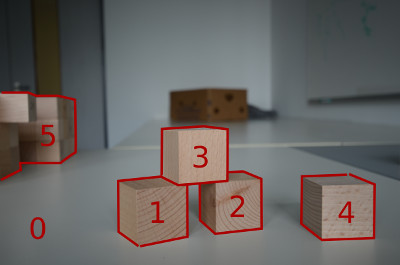
\includegraphics[width=\textwidth]{./figures/sec/secexample_blocksmarkednumbered.jpg}
    \subcaption{Manually segmented example scene of blocks on a table.}
    \label{fig:sec_secexample_blocksmarkednumbered}
  \end{subfigure}
  \hfill
  \begin{subfigure}[t]{0.475\textwidth}
    \raisebox{0.5cm}{%
      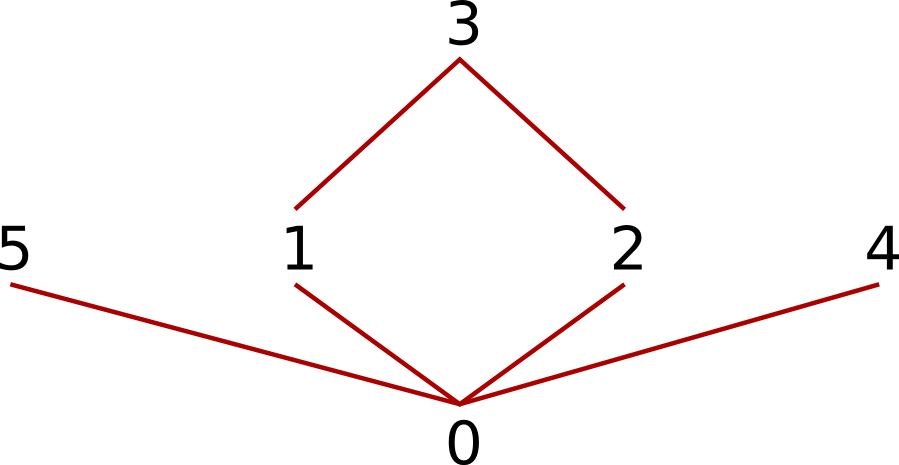
\includegraphics[width=\textwidth]{./figures/sec/secexample_graph.png}%
    }
    \caption{Extracted graph representation of the scene.}
    \label{fig:sec_secexample_graph}
  \end{subfigure}
  \caption{A visualization of an object graph. Computer vision identifies and separates objects and their relative structure to each other (left image). One Semantic Event Graph (right image) results directly from the structure. Please note that multiple roots for one graph are allowed.}
  \label{fig:sec_secexample}
\end{figure}

\begin{align}
  \bordermatrix{
    & 0 & 1 & 2 & 3 & 4 & 5\cr
    0 & \colorbox{green120}{0} & \textup{T} & \textup{T} & \textup{N} & \textup{T} & \textup{T}\cr
    1 & \textup{T} & \colorbox{green120}{1} & \textup{N} & \textup{T} & \textup{N} & \textup{N}\cr
    2 & \textup{T} & \textup{N} & \colorbox{green120}{2} & \textup{T} & \textup{N} & \textup{N}\cr
    3 & \textup{N} & \textup{T} & \textup{T} & \colorbox{green120}{3} & \textup{N} & \textup{N}\cr
    4 & \textup{T} & \textup{N} & \textup{N} & \textup{N} & \colorbox{green120}{4} & \textup{N}\cr
    5 & \textup{T} & \textup{N} & \textup{N} & \textup{N} & \textup{N} & \colorbox{green120}{5}\cr
    },
\end{align}

where ``T'' marks an edge and ``N'' stands for a not-touching relation. 
This matrix is called \gls{ac:sem}.
It is symmetric and contains the object identifiers on the diagonal (marked in green).
Additionally to touching and not-touching, there may be an edge named \emph{absent} ``A'', which is used when new objects come into the scene; for example when a cucumber is being cut into two pieces, or when an object is uncovered during a scene.
Now, each change in the scene corresponds to a change in the touching relation and therefore results in a new matrix. 
A list of \glspl{ac:sem} is called a \acrlong{ac:sec}.
The camera frame, in which the change of relation occurs is called a keyframe.
\Glspl{ac:sec} are independent of the time domain and the robotic hardware. 

\begin{figure}
  \centering
  % Define block styles
\tikzstyle{block} = [rectangle, fill=white, text centered, minimum height=0.5em, rounded corners=true]
\tikzstyle{blockBox} = [draw, rectangle, fill=white, minimum height=3cm, minimum width=4.5cm, text width=1em, text centered, rounded corners=true]

\tikzstyle{blockSupP} = [draw, rectangle, fill=red1!20,   minimum height=0.52cm, minimum width=1.3cm, text width=1em, text centered, rounded corners=true]
\tikzstyle{blockSupM} = [draw, rectangle, fill=green1!20, minimum height=0.52cm, minimum width=4cm, text width=3.8cm, text centered, rounded corners=true]
\tikzstyle{blockSupS} = [draw, rectangle, fill=blue1!20,  minimum height=0.52cm, minimum width=1.3cm, text width=1em, text centered, rounded corners=true]
\tikzstyle{blockSup}  = [draw, rectangle, fill=red1!20,   minimum height=0.52cm, minimum width=3.1cm, text width=3.1cm, text centered, rounded corners=true]

\tikzstyle{blockCon} = [draw, rectangle, fill=white, minimum height=0.5cm, minimum width=1cm, text width=0.6cm, text centered, rounded corners=true]
\tikzstyle{blockP} = [draw, rectangle, fill=red1!40, minimum height=0.52cm, minimum width=0.6cm, text width=1em, text centered, rounded corners=true]
\tikzstyle{blockM} = [draw, rectangle, fill=green1!40, minimum height=0.52cm, minimum width=1.6cm, text width=1.6cm, text centered, rounded corners=true]
\tikzstyle{blockS} = [draw, rectangle, fill=blue1!40, minimum height=0.52cm, minimum width=0.6cm, text width=1em, text centered, rounded corners=true]
\tikzstyle{blockL} = [draw, rectangle, fill=black!20, minimum height=0.52cm, minimum width=0.6cm, text width=1em, text centered, rounded corners=true]
\tikzstyle{arrow} = [draw, -latex]
\tikzstyle{line} = [draw]

\definecolor{red1}{RGB}{160,0,0}
\definecolor{green1}{RGB}{0,160,0}
\definecolor{blue1}{RGB}{0,0,160}

\pgfdeclareimage[width=0.6cm]{hand}{./figures/sec/robothand.jpg}

	      
\begin{tikzpicture}[node distance=6em, auto]
	%%%%%%%%%%%%%%%%%%%%%%%%%%%%%%%%%%%%%%%%%%%%%%%%%%%%%%%%%%%%%%%%%%%%%%%%%%%%%%%%%%%%%%%%%%%%%%%%%%%%%%
	% First line
	\node [blockBox] (p11) {};
	\node [blockBox, right of=p11, node distance=5cm] (p12) {};
	\node [blockBox, right of=p12, node distance=5cm] (p13) {};

	% Panel number
	\node[below left] at (p11.north east) {1};
	\node[below left] at (p12.north east) {2};
	\node[below left] at (p13.north east) {3};

	% Panel 11
	\node[above right, xshift=0.25cm, blockSupM] at (p11.south west) (p11_Sup) {\small{main support (id=0)}};
	\node[above of=p11_Sup, blockM, node distance=0.67cm, xshift=-0.6cm] (p11_m) {\small{m (id=1)}};
	\node[left of=p11_m, node distance=0.7cm, yshift=1.0cm] (p11_h) {\pgfuseimage{hand}};

	% Panel 12
	\node[above right, xshift=0.25cm, blockSupM] at (p12.south west) (p12_Sup) {\small{main support (id=0)}};
	\node[above of=p12_Sup, blockM, node distance=0.67cm, xshift=-0.6cm] (p12_m) {\small{m (id=1)}};
	\node[left of=p12_m, node distance=1.2cm, yshift=0.3cm] (p12_h) {\pgfuseimage{hand}};

	\node[above of=p12_Sup, blockM, node distance=0.67cm, xshift=-0.6cm] (p12_m) {\small{m (id=1)}};

	% Panel 13
	\node[above right, xshift=0.25cm, blockSupM] at (p13.south west) (p13_Sup) {\small{main support (id=0)}};
	\node[above of=p13_Sup, blockM, node distance=0.67cm, xshift=0.9cm] (p13_m) {\small{m (id=1)}};
	\node[left of=p13_m, node distance=1.5cm, yshift=0.9cm] (p13_h) {\pgfuseimage{hand}};

  % Trajectory
  %\draw[dashed, line width=0.25mm] ([xshift=-1.4cm, yshift=1.3cm]p11_Sup.north) to[rounded corners=20pt] ([xshift=-2.1cm, yshift=0.5cm]p11_Sup.north) to[rounded corners=20pt] ([xshift=0.0cm, yshift=0.5cm]p11_Sup.north) to[rounded corners=20pt] ([xshift=-0.6cm, yshift=1.2cm]p11_Sup.north);

  \draw[dashed, line width=0.25mm] ([xshift=-1.4cm, yshift=1.3cm]p12_Sup.north) to[rounded corners=20pt] ([xshift=-1.8cm, yshift=0.7cm]p12_Sup.north);

  \draw[dashed, line width=0.25mm] ([xshift=-1.4cm, yshift=1.3cm]p13_Sup.north) to[rounded corners=20pt] ([xshift=-2.1cm, yshift=0.5cm]p13_Sup.north) to[rounded corners=20pt] ([xshift=0.0cm, yshift=0.5cm]p13_Sup.north) to[rounded corners=20pt] ([xshift=-0.6cm, yshift=1.2cm]p13_Sup.north);


	%%%%%%%%%%%%%%%%%%%%%%%%%%%%%%%%%%%%%%%%%%%%%%%%%%%%%%%%%%%%%%%%%%%%%%%%%%%%%%%%%%%%%%%%%%%%%%%%%%%%%%
	% Second line

  \node[block, below of=p11,    node distance=4.5cm] (p21_ms) {main support, id=0};
  \node[block, above of=p21_ms, node distance=1cm] (p21_m) {main, id=1};
  \node[block, above of=p21_ms, node distance=2cm] (p21_hand) {robot hand, id=2};
  \draw[line] (p21_ms.north) to (p21_m.south);

  \node[block, below of=p12,    node distance=4.5cm] (p22_ms) {main support, id=0};
  \node[block, above of=p22_ms, node distance=1cm] (p22_m) {main, id=1};
  \node[block, above of=p22_ms, node distance=2cm] (p22_hand) {robot hand, id=2};
  \draw[line] (p22_ms.north) to (p22_m.south);
  \draw[line] (p22_m.north) to (p22_hand.south);

  \node[block, below of=p13,    node distance=4.5cm] (p23_ms) {main support, id=0};
  \node[block, above of=p23_ms, node distance=1cm] (p23_m) {main, id=1};
  \node[block, above of=p23_ms, node distance=2cm] (p23_hand) {robot hand, id=2};
  \draw[line] (p23_ms.north) to (p23_m.south);


	%%%%%%%%%%%%%%%%%%%%%%%%%%%%%%%%%%%%%%%%%%%%%%%%%%%%%%%%%%%%%%%%%%%%%%%%%%%%%%%%%%%%%%%%%%%%%%%%%%%%%%
	% Third line

    \node[block, below of=p21_ms, node distance=2.25cm] (p31) {
      $\bordermatrix{
        & 0 & 1 & 2\cr
        0 & \colorbox{green120}{0}  & \textup{T}              & \textup{N}\cr
        1 & \textup{T}              & \colorbox{green120}{1}  & \textup{N}\cr
        2 & \textup{N}              & \textup{N}              & \colorbox{green120}{2}\cr        
      }$
    };

    \node[block, below of=p22_ms, node distance=2.25cm] (p31) {
      $\bordermatrix{
        & 0 & 1 & 2\cr
        0 & \colorbox{green120}{0}  & \textup{T}              & \textup{N}\cr
        1 & \textup{T}              & \colorbox{green120}{1}  & \textup{T}\cr
        2 & \textup{N}              & \textup{T}              & \colorbox{green120}{2}\cr        
      }$
    };

    \node[block, below of=p23_ms, node distance=2.25cm] (p31) {
      $\bordermatrix{
        & 0 & 1 & 2\cr
        0 & \colorbox{green120}{0}  & \textup{T}              & \textup{N}\cr
        1 & \textup{T}              & \colorbox{green120}{1}  & \textup{N}\cr
        2 & \textup{N}              & \textup{N}              & \colorbox{green120}{2}\cr        
      }$
    };
\end{tikzpicture}

  \caption{An example showing a pushing action in the \gls{ac:sec} domain. The first row shows a pictogram view of the action. The \emph{main} object, denoted with ``m'', sits on top the ``main support'' and the robot is not touching the \emph{main} object. In the second keyframe the robot touches the \emph{main} object and pushes it to the right. The robot's trajectory is marked with a dashed line. However, this trajectory information is not encoded in the \gls{ac:sec}. In the third keyframe the robot hand is removed from the \emph{main} object. The middle row holds a graph representation of the touching and not-touching relations; touching relations are marked with a line. In the bottom row the graph is represented as \glspl{ac:sem}. All three matrices hold a lot of static information. Therefore, a short form, which removes all static information, is introduced. For this example one could also write: ``main object -- robot hand: N~T~N''.}
  \label{fig:sec_examplescenario_pushing}
\end{figure}

A second (and also artificial) example of a \action{pushing} action is shown in \figref{fig:sec_examplescenario_pushing}.
A robot pushes the \emph{main} object ``m'' along its support.
In the first keyframe, there is only one touching connection between the object and its support, which is shown in the graph below the pictogram and also reflected in the \gls{ac:sem} below the graph.
Next, the robot begins to touch the \emph{main} object and holds that connection for the entire trajectory, \ie for a longer period of time.
The last (third) keyframe is generated as soon as the robot looses contact to the \emph{main} object.

A third example of a \action{pick and place} action is displayed in \figref{fig:sec_examplescenario_pickandplace}; it is derived from a real world experiment.
In the first keyframe an apple is on top of a plate and the robot hand hovers above the table.
In the next keyframes it holds the apple, lifts it off the plate, and places it on the table.
This sequence of touching/non-touching relations is unique for this type of action.
If in this scene the robot were to push the apple on the plate, the graph sequence would look differently.
While the first two keyframes would look like the pick-and-place example, the third keyframe would be equal to the first: The robot hand hovering in the air.
Immediately one problem becomes apparent: In both examples the first two keyframes are alike, even though in one example the apple is picked and in another example it is pushed.
Therefore, reliable action recognition is only possible on a very late stage of action execution.

\begin{figure}[]
  \centering
  \begin{subfigure}[t]{0.475\textwidth}
    \centering
    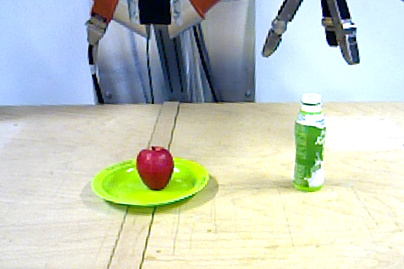
\includegraphics[width=\textwidth]{./figures/sec/scenario/darktable_exported/frame0493.jpg}
    \subcaption{Keyframe 1, this is the very first camera frame.}
    \label{fig:sec_examplescenario_pickandplace_1j}
  \end{subfigure}
  \hfil
  \begin{subfigure}[t]{0.475\textwidth}
    \centering
    % Define block styles
\tikzstyle{block} = [rectangle, fill=white, text centered, rounded corners]
\tikzstyle{arrow} = [draw]
\usetikzlibrary{matrix}

\pgfdeclareimage[width=11em]{ImBlock}{./figures/sec/secexample_blocksmarkednumbered.jpg}
\pgfdeclareimage[width=11em]{ImGraph}{./figures/sec/secexample_graph.png}

\definecolor{red1}{RGB}{160,0,0}
\definecolor{green1}{RGB}{0,160,0}
\definecolor{blue1}{RGB}{0,0,160}

	      
\begin{tikzpicture}[node distance=1cm, auto]
    \node[block] (table) {Table};
    \node[block, above of=table, xshift=-2cm, color=white] (appleW) {Robot hand};

    \node[block, above of=table, xshift=2cm] (bottle) {Bottle};
    \node[block, above of=table, xshift=-2cm] (plate) {Plate};
    \node[block, above of=plate] (apple) {Apple};
    \node[block, above of=apple, xshift=2cm] (hand) {Robot hand};

    % lines
    \draw [arrow] (table.north) to (plate.south);
    \draw [arrow] (table.north) to (bottle.south);
    \draw [arrow] (plate.north) to (apple.south);

    % alignment
    \node[block, below of=table, color=white, node distance=0.4cm] (appleW) {Robot hand};
    \node[block] (table) {Table};
\end{tikzpicture}
%
    \subcaption{Graph representation of Keyframe 1.}
    \label{fig:sec_examplescenario_pickandplace_1t}
  \end{subfigure}\\%
  \begin{subfigure}[t]{0.475\textwidth}
    \centering
    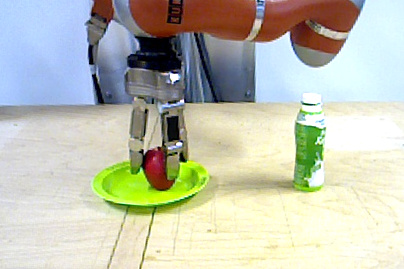
\includegraphics[width=\textwidth]{./figures/sec/scenario/darktable_exported/frame0837.jpg}
    \subcaption{Keyframe 2, the robot arm touches the apple.}
    \label{fig:sec_examplescenario_pickandplace_2j}
  \end{subfigure}
  \hfil
  \begin{subfigure}[t]{0.475\textwidth}
    \centering
    % Define block styles
\tikzstyle{block} = [rectangle, fill=white, text centered, rounded corners]
\tikzstyle{arrow} = [draw]
\usetikzlibrary{matrix}

\pgfdeclareimage[width=11em]{ImBlock}{./figures/sec/secexample_blocksmarkednumbered.jpg}
\pgfdeclareimage[width=11em]{ImGraph}{./figures/sec/secexample_graph.png}

\definecolor{red1}{RGB}{160,0,0}
\definecolor{green1}{RGB}{0,160,0}
\definecolor{blue1}{RGB}{0,0,160}

	      
\begin{tikzpicture}[node distance=1cm, auto]
    \node[block] (table) {Table};
    \node[block, above of=table, xshift=-2cm, color=white] (appleW) {Robot hand};

    \node[block, above of=table, xshift=2cm] (bottle) {Bottle};
    \node[block, above of=table, xshift=-2cm] (plate) {Plate};
    \node[block, above of=plate] (apple) {Apple};
    \node[block, above of=apple] (hand) {Robot hand};

    % lines
    \draw [arrow] (table.north) to (plate.south);
    \draw [arrow] (table.north) to (bottle.south);
    \draw [arrow] (plate.north) to (apple.south);
    \draw [arrow] (apple.north) to (hand.south);

    % alignment
    \node[block, below of=table, color=white, node distance=0.4cm] (appleW) {Robot hand};
    \node[block] (table) {Table};
\end{tikzpicture}
%
    \subcaption{Graph representation of Keyframe 2.}
    \label{fig:sec_examplescenario_pickandplace_2t}
  \end{subfigure}\\%
  \begin{subfigure}[t]{0.475\textwidth}
    \centering
    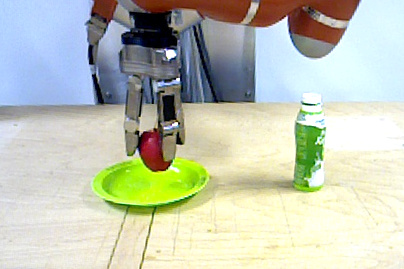
\includegraphics[width=\textwidth]{./figures/sec/scenario/darktable_exported/frame0893.jpg}
    \subcaption{Keyframe 3, the robot lifts the apple of the plate.}
    \label{fig:sec_examplescenario_pickandplace_3j}
  \end{subfigure}
  \hfil
  \begin{subfigure}[t]{0.475\textwidth}
    \centering
    % Define block styles
\tikzstyle{block} = [rectangle, fill=white, text centered, rounded corners]
\tikzstyle{arrow} = [draw]
\usetikzlibrary{matrix}

\pgfdeclareimage[width=11em]{ImBlock}{./figures/sec/secexample_blocksmarkednumbered.jpg}
\pgfdeclareimage[width=11em]{ImGraph}{./figures/sec/secexample_graph.png}

\definecolor{red1}{RGB}{160,0,0}
\definecolor{green1}{RGB}{0,160,0}
\definecolor{blue1}{RGB}{0,0,160}

	      
\begin{tikzpicture}[node distance=1cm, auto]
    \node[block] (table) {Table};
    \node[block, above of=table, xshift=-2cm, color=white] (appleW) {Robot hand};

    \node[block, above of=table, xshift=2cm] (bottle) {Bottle};
    \node[block, above of=table, xshift=-2cm] (plate) {Plate};
    \node[block, above of=plate] (apple) {Apple};
    \node[block, above of=apple] (hand) {Robot hand};

    % lines
    \draw [arrow] (table.north) to (plate.south);
    \draw [arrow] (table.north) to (bottle.south);
    \draw [arrow] (apple.north) to (hand.south);

    % alignment
    \node[block, below of=table, color=white, node distance=0.4cm] (appleW) {Robot hand};
    \node[block] (table) {Table};
\end{tikzpicture}
%
    \subcaption{Graph representation of Keyframe 3.}
    \label{fig:sec_examplescenario_pickandplace_3t}
  \end{subfigure}
\end{figure}
\begin{figure}[]\ContinuedFloat
  \centering
  \begin{subfigure}[t]{0.475\textwidth}
    \centering
    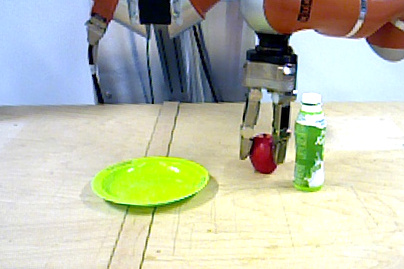
\includegraphics[width=\textwidth]{./figures/sec/scenario/darktable_exported/frame1095.jpg}
    \subcaption{Keyframe 4, the apple is placed on the table.}
    \label{fig:sec_examplescenario_pickandplace_4j}
  \end{subfigure}
  \hfil
  \begin{subfigure}[t]{0.475\textwidth}
    \centering
    % Define block styles
\tikzstyle{block} = [rectangle, fill=white, text centered, rounded corners]
\tikzstyle{arrow} = [draw]
\usetikzlibrary{matrix}

\pgfdeclareimage[width=11em]{ImBlock}{./figures/sec/secexample_blocksmarkednumbered.jpg}
\pgfdeclareimage[width=11em]{ImGraph}{./figures/sec/secexample_graph.png}

\definecolor{red1}{RGB}{160,0,0}
\definecolor{green1}{RGB}{0,160,0}
\definecolor{blue1}{RGB}{0,0,160}

	      
\begin{tikzpicture}[node distance=1cm, auto]
    \node[block] (table) {Table};
    \node[block, above of=table, xshift=-2cm, color=white] (appleW) {Robot hand};

    \node[block, above of=table, xshift=2cm] (bottle) {Bottle};
    \node[block, above of=table, xshift=-2cm] (plate) {Plate};
    \node[block, above of=table] (apple) {Apple};
    \node[block, above of=apple] (hand) {Robot hand};

    % lines
    \draw [arrow] (table.north) to (plate.south);
    \draw [arrow] (table.north) to (bottle.south);
    \draw [arrow] (table.north) to (apple.south);
    \draw [arrow] (apple.north) to (hand.south);

    % alignment
    \node[block, below of=table, color=white, node distance=0.4cm] (appleW) {Robot hand};
    \node[block] (table) {Table};
\end{tikzpicture}
%
    \subcaption{Graph representation of Keyframe 4.}
    \label{fig:sec_examplescenario_pickandplace_4t}
  \end{subfigure}\\%
  \begin{subfigure}[t]{0.475\textwidth}
    \centering
    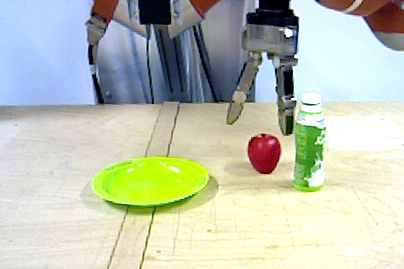
\includegraphics[width=\textwidth]{./figures/sec/scenario/darktable_exported/frame1174.jpg}
    \subcaption{Keyframe 5, the robot arm lets go of the object.}
    \label{fig:sec_examplescenario_pickandplace_5j}
  \end{subfigure}
  \hfil
  \begin{subfigure}[t]{0.475\textwidth}
    \centering
    % Define block styles
\tikzstyle{block} = [rectangle, fill=white, text centered, rounded corners]
\tikzstyle{arrow} = [draw]
\usetikzlibrary{matrix}

\pgfdeclareimage[width=11em]{ImBlock}{./figures/sec/secexample_blocksmarkednumbered.jpg}
\pgfdeclareimage[width=11em]{ImGraph}{./figures/sec/secexample_graph.png}

\definecolor{red1}{RGB}{160,0,0}
\definecolor{green1}{RGB}{0,160,0}
\definecolor{blue1}{RGB}{0,0,160}

	      
\begin{tikzpicture}[node distance=1cm, auto]
    \node[block] (table) {Table};
    \node[block, above of=table, xshift=-2cm, color=white] (appleW) {Robot hand};

    \node[block, above of=table, xshift=2cm] (bottle) {Bottle};
    \node[block, above of=table, xshift=-2cm] (plate) {Plate};
    \node[block, above of=table] (apple) {Apple};
    \node[block, above of=apple] (hand) {Robot hand};

    % lines
    \draw [arrow] (table.north) to (plate.south);
    \draw [arrow] (table.north) to (bottle.south);
    \draw [arrow] (table.north) to (apple.south);

    % alignment
    \node[block, below of=table, color=white, node distance=0.4cm] (appleW) {Robot hand};
    \node[block] (table) {Table};
\end{tikzpicture}
%
    \subcaption{Graph representation of Keyframe 5.}
    \label{fig:sec_examplescenario_pickandplace_5t}
  \end{subfigure}%
  \caption{Frames from a robot demonstration: The robot picks an apple from a plate and places it on the table. The corresponding graph representation is given on the right side.}
  \label{fig:sec_examplescenario_pickandplace}
\end{figure}

Another problem surfaces, when thinking about the \action{scratching} action: \ie scratching with a robot finger on paper.
This action is indistinguishable from the pushing action on the \gls{ac:sec} domain, they only differ in the robot hands trajectory.
Both actions last for three keyframes where the first and last keyframes are identical; in the second keyframe the robot touches the object.
Here, it is important to note that \glspl{ac:sec} do not store trajectory or time information.
While on the one side this seems like a disadvantage, it is in fact the biggest strength of the \gls{ac:sec} domain.
Trajectory information is hardware dependent and therefore robot specific.
Using \glspl{ac:sec} one can recognize~\cite{aksoytamosiunaitevuga2013}, learn~\cite{aksoy2011learning, aksoydellentamosiunaite2011}, and repeat~\cite{aksoydellentamosiunaite2011} a very wide range of actions.
Furthermore, actions can be enriched using action-related trajectory information and thus be used for bootstrap learning~\cite{aksoytamosiunaitevuga2013}.

Still, not necessarily all actions a human can perform may be encoded using \glspl{ac:sec}.
For some actions higher level knowledge is needed.
As an example of these actions, \action{spreading the marmelade} may serve as an example.
It first depends on the trajectory's velocity and second on the size of the bread, which cannot be described based on \glspl{ac:sec} alone.
To overcome some of these shortcomings of \glspl{ac:sec}, in the next chapter pose information is added.
This will allow for a framework to execute actions, which generalizes while still being independent of the time domain.

\subsection{Enriched Semantic Event Chains}
\label{ssec:action_methods_enrichedsemanticeventchains}

As seen in the last chapter, for robot execution of Semantic Event Chains, some additional pose information must be included.
Therefore, \glspl{ac:sec} are enriched by higher level structural information.
Each entry of one keyframe matrix now may not only hold ``T'', ``N'', or ``A'', but also an additional vector containing the relative pose between the two objects.
An example can be seen in \figref{fig:sec_examplescenario_pushing_firstkeyframe}, which is similar to the first keyframe in the example \figref{fig:sec_examplescenario_pushing}, but introduces an additional coordinate system.
Following this approach, the Semantic Event Chain turns into an \gls{ac:esec} as

\begin{figure}
  \centering
  % Define block styles
\tikzstyle{block} = [rectangle, fill=white, text centered, minimum height=0.5em, rounded corners=true]
\tikzstyle{blockBox} = [draw, rectangle, fill=white, minimum height=2.8cm, minimum width=6.0cm, text width=1em, text centered, rounded corners=true]

\tikzstyle{blockSupP} = [draw, rectangle, fill=red1!20,   minimum height=0.52cm, minimum width=1.3cm, text width=1em, text centered, rounded corners=true]
\tikzstyle{blockSupM} = [draw, rectangle, fill=green1!20, minimum height=0.52cm, minimum width=3.1cm, text width=3.1cm, text centered, rounded corners=true]
\tikzstyle{blockSupS} = [draw, rectangle, fill=blue1!20,  minimum height=0.52cm, minimum width=1.3cm, text width=1em, text centered, rounded corners=true]
\tikzstyle{blockSup}  = [draw, rectangle, fill=red1!20,   minimum height=0.52cm, minimum width=3.1cm, text width=3.1cm, text centered, rounded corners=true]

\tikzstyle{blockCon} = [draw, rectangle, fill=white, minimum height=0.5cm, minimum width=1cm, text width=0.6cm, text centered, rounded corners=true]
\tikzstyle{blockP} = [draw, rectangle, fill=red1!40, minimum height=0.52cm, minimum width=0.6cm, text width=1em, text centered, rounded corners=true]
\tikzstyle{blockM} = [draw, rectangle, fill=green1!40, minimum height=0.52cm, minimum width=0.6cm, text width=1em, text centered, rounded corners=true]
\tikzstyle{blockS} = [draw, rectangle, fill=blue1!40, minimum height=0.52cm, minimum width=0.6cm, text width=1em, text centered, rounded corners=true]
\tikzstyle{blockL} = [draw, rectangle, fill=black!20, minimum height=0.52cm, minimum width=0.6cm, text width=1em, text centered, rounded corners=true]
\tikzstyle{arrow} = [draw, -latex]
\tikzstyle{line} = [draw]

\definecolor{red1}{RGB}{160,0,0}
\definecolor{green1}{RGB}{0,160,0}
\definecolor{blue1}{RGB}{0,0,160}

\pgfdeclareimage[width=0.6cm]{hand}{./figures/sec/robothand.jpg}

	      
\begin{tikzpicture}[node distance=6em, auto]
	%%%%%%%%%%%%%%%%%%%%%%%%%%%%%%%%%%%%%%%%%%%%%%%%%%%%%%%%%%%%%%%%%%%%%%%%%%%%%%%%%%%%%%%%%%%%%%%%%%%%%%
	% Panel
	\node [blockBox] (p11) {};

	\node[above right, xshift=2.2cm, blockSupM, minimum width=3cm] at (p11.south west) (p11_Sup) {\small{main support}};
	\node[above of=p11_Sup, blockM, node distance=0.58cm, xshift=-0.8cm] (p11_m) {\small{m}};
	\node[left of=p11_m, node distance=0.8cm, yshift=0.6cm] (p11_h) {\pgfuseimage{hand}};

    % Text
    \node[right of=p11_Sup, node distance=0.8cm, xshift=0.2cm, yshift=0.8cm] (p11_Sup_t) {id=0};
    \node[right of=p11_m,   node distance=0.8cm, xshift=0.0cm, yshift=0.8cm] (p11_m_t) {id=1};
    \node[left of=p11_h,    node distance=0.8cm, xshift=-0.1cm, yshift=0.8cm] (p11_h_t) {id=2};

    % Lines
    \draw[line] (p11_Sup_t.south) to ++(-0.1cm,-0.25cm);
    \draw[line] (p11_m_t.south) to ++(-0.5cm,-0.3cm);
    \draw[line] (p11_h_t.south) to ++( 0.5cm,-0.3cm);

    \draw [<->] (-2.7cm,-0.7cm) node (yaxis) [above] {$z$}
                |- (-2.3cm,-1.1cm) node (xaxis) [right] {$x$};


	%%%%%%%%%%%%%%%%%%%%%%%%%%%%%%%%%%%%%%%%%%%%%%%%%%%%%%%%%%%%%%%%%%%%%%%%%%%%%%%%%%%%%%%%%%%%%%%%%%%%%%
	% Matrix

    \node[block, right of=p11_m, yshift=0.5cm, node distance=6.0cm] (p31) {
      $\bordermatrix{
          & 0 & 1 & 2\cr
        0 & 0           & \textup{T}    & \textup{N}\cr
        1 & \textup{T}  & 1             & \textup{N}\cr
        2 & \textup{N}  & \textup{N}    & 2\cr        
      }$
    };
\end{tikzpicture}

  \caption{This is the same scene as shown in \figref{fig:sec_examplescenario_pushing} --- a robot pushing the \emph{main} object along its support. Please note the coordinate system, which is used when the keyframe matrix on the right is enriched by relative pose information, see \eqnref{eqn:sec_enriched_2d}. For clarity only two dimensions are used here (where $y=0$).}
  \label{fig:sec_examplescenario_pushing_firstkeyframe}
\end{figure}

\begin{align}
  \bordermatrix{
    & 0 & 1 & 2\cr
    0 & \colorbox{green120}{0}    & (\textup{T},~(0,~0,~1))         & (\textup{N},~(0,~0,~1))\cr
    1 & (\textup{T},~(0,~0,~-1))  & \colorbox{green120}{1}          & (\textup{N},~(-0.71,~0,~0.71))\cr
    2 & (\textup{N},~(0,~0,~-1))  & (\textup{N},~(0.71,~0,~-0.71))  & \colorbox{green120}{2}\cr
    },
  \label{eqn:sec_enriched_2d}
\end{align}

where the ID is marked in green.
A more general form for the keyframe matrix $\underline{K}$ is

\begin{align}
  \underline{K} := \begin{pmatrix}
    a_{0,0}         & \vec{a}_{1,0} & \cdots & \vec{a}_{i,0}    & \cdots & \vec{a}_{N,0}\\
    \vec{a}_{0,1}   & \ddots        &        &                  &        & \vdots\\
    \vdots          &               &        &                  &        &\\
    \vec{a}_{0,j}   &               &        &                  &        &\\
    \vdots          &               &        &                  &        &\\
    \vec{a}_{0,N}   & \cdots        &        &                  &        & a_{N,N}\\
  \end{pmatrix}
  \label{eqn:sec_enriched_general}
\end{align}

where

\begin{align}
  a_{i,i} := i
\end{align}

and for $i\neq j$

\begin{align}
  \vec{a}_{i,j} := \left( r,~\vec{p}_0,~\cdots,~\vec{p}_m,~\cdots,~\vec{p}_k\right).
\end{align}

The scalar entries ``T'', ``N'', and ``A'' are replaced by vectors of the form $(r,~\vec{p}_m)$, where relation $r \in \{\textup{T},~\textup{N},~\textup{A}\}$ and $\vec{p}_m \in \Re^d$.
The vector $\vec{p}_m$ is normalized to unit length such that $|\vec{p}_m| \overset{!}{=} 1$.

One might expect that one vector is enough to define the relative pose between two objects.
However, using only one vector often does not catch the shape of the other object.
For example, one might imagine a simple cube, surrounded by an L-shaped block.
Here, at least two vectors are needed to describe the directions, in which the cube must not be moved in order to not touch the L-shaped block.
In these experiments, as will be shown below, up to $k=8$ different pose vectors per relation are allowed.
Below, an algorithm for 3d geometrical reasoning is devised, which will output these vectors.
Parts of this section have been published in~\textcite{reichaeinwoergoetter2018}.




%\subsection{3d Geometrical reasoning}

First, please imagine a \action{pick \& place} action.
It is quite difficult to determine the ``correct'' rotation of the hand to pick up an object.
Additionally, if the scene is cluttered, it is often hard to tell in which direction the hand should move to lift the object and to not touch any other objects.
Here, a geometrical reasoning algorithm is needed, which will output this information.
As already mentioned, there is --- due to Semantic Event Chains --- a good understanding of top and bottom of the scene.
However, the question which objects are left and right of the \emph{main} object remain.
Most certainly the robot will also encounter objects of different sizes and shapes, which must be taken into account, too.

Currently, the vast field of different robot hardware and use cases has shown that geometric reasoning algorithms do not generalize well.
For example, in~\cite{havur2014geometric} the focus lies on computing efficiently the relative position of multiple moving objects to each other; results are shown only in simulation.
In~\cite{erdem2011combining} geometric reasoning is combined with a causal symbolic planner, which in turn is used in an industrial use case.
On a more abstract layer,~\cite{marin2009towards} defines attention space using low level geometric features.
Thresholds define a space around the robot for human-robot collaboration.
In~\cite{subburaj2007high, subburaj2009automated, lee2009geometric} geometric reasoning is used to infer information about local structures.
These are used in medical robots~\cite{subburaj2007high, subburaj2009automated}.

As of today there is no labeled benchmark for geometric reasoning in real world scenarios.
Thus quantitative evaluation is not very meaningful as one would need to generate the ground truth first.
This, however, is hardware specific, robot dependent, and does not generalize.

\begin{figure}[]
  \begin{subfigure}[]{0.4\textwidth}
    \centering
    \includegraphics[height=4cm]{./figures/sec/geometrical_reasoning/blocks.png}
    \caption{Two blocks serve as an example for geometric reasoning. Here, one is interested in which direction the green cube can be moved without touching the blue one.}
    \label{fig:sec_enriched_geometricalreasoning_approach_overview_blocks}
  \end{subfigure}
  \hfill
  \begin{subfigure}[]{0.55\textwidth}
    \centering
    \begin{tikzpicture}[gnuplot]
%% generated with GNUPLOT 5.2p2 (Gentoo revision r0) (Lua 5.1; terminal rev. 99, script rev. 102)
%% Fri 15 Jun 2018 09:58:01 AM CEST
\path (0.000,0.000) rectangle (8.400,3.400);
\gpcolor{color=gp lt color axes}
\gpsetlinetype{gp lt axes}
\gpsetdashtype{gp dt axes}
\gpsetlinewidth{0.50}
\draw[gp path] (2.361,0.985)--(2.361,3.091);
\gpcolor{color=gp lt color border}
\gpsetlinetype{gp lt border}
\gpsetdashtype{gp dt solid}
\gpsetlinewidth{1.00}
\draw[gp path] (2.361,0.985)--(2.361,1.165);
\draw[gp path] (2.361,3.091)--(2.361,2.911);
\node[gp node center] at (2.361,0.677) {$5$};
\gpcolor{color=gp lt color axes}
\gpsetlinetype{gp lt axes}
\gpsetdashtype{gp dt axes}
\gpsetlinewidth{0.50}
\draw[gp path] (4.131,0.985)--(4.131,3.091);
\gpcolor{color=gp lt color border}
\gpsetlinetype{gp lt border}
\gpsetdashtype{gp dt solid}
\gpsetlinewidth{1.00}
\draw[gp path] (4.131,0.985)--(4.131,1.165);
\draw[gp path] (4.131,3.091)--(4.131,2.911);
\node[gp node center] at (4.131,0.677) {$10$};
\gpcolor{color=gp lt color axes}
\gpsetlinetype{gp lt axes}
\gpsetdashtype{gp dt axes}
\gpsetlinewidth{0.50}
\draw[gp path] (5.900,0.985)--(5.900,3.091);
\gpcolor{color=gp lt color border}
\gpsetlinetype{gp lt border}
\gpsetdashtype{gp dt solid}
\gpsetlinewidth{1.00}
\draw[gp path] (5.900,0.985)--(5.900,1.165);
\draw[gp path] (5.900,3.091)--(5.900,2.911);
\node[gp node center] at (5.900,0.677) {$15$};
\draw[gp path] (0.768,3.091)--(0.768,0.985)--(7.847,0.985)--(7.847,3.091)--cycle;
\node[gp node center,rotate=-270] at (0.276,2.038) {Count};
\node[gp node center] at (4.307,0.215) {Binned distance [a.u.]};
\gpfill{rgb color={0.667,0.000,0.000}} (0.856,0.985)--(1.034,0.985)--(1.034,1.324)--(0.856,1.324)--cycle;
\gpcolor{rgb color={0.667,0.000,0.000}}
\draw[gp path] (0.856,0.985)--(0.856,1.323)--(1.033,1.323)--(1.033,0.985)--cycle;
\gpfill{rgb color={0.667,0.000,0.000}} (1.210,0.985)--(1.388,0.985)--(1.388,1.924)--(1.210,1.924)--cycle;
\draw[gp path] (1.210,0.985)--(1.210,1.923)--(1.387,1.923)--(1.387,0.985)--cycle;
\gpfill{rgb color={0.667,0.000,0.000}} (1.564,0.985)--(1.742,0.985)--(1.742,2.323)--(1.564,2.323)--cycle;
\draw[gp path] (1.564,0.985)--(1.564,2.322)--(1.741,2.322)--(1.741,0.985)--cycle;
\gpfill{rgb color={0.000,0.667,0.000}} (1.918,0.985)--(2.096,0.985)--(2.096,2.527)--(1.918,2.527)--cycle;
\gpcolor{rgb color={0.000,0.667,0.000}}
\draw[gp path] (1.918,0.985)--(1.918,2.526)--(2.095,2.526)--(2.095,0.985)--cycle;
\gpfill{rgb color={0.000,0.667,0.000}} (2.272,0.985)--(2.450,0.985)--(2.450,2.474)--(2.272,2.474)--cycle;
\draw[gp path] (2.272,0.985)--(2.272,2.473)--(2.449,2.473)--(2.449,0.985)--cycle;
\gpfill{rgb color={0.000,0.667,0.000}} (2.626,0.985)--(2.804,0.985)--(2.804,2.279)--(2.626,2.279)--cycle;
\draw[gp path] (2.626,0.985)--(2.626,2.278)--(2.803,2.278)--(2.803,0.985)--cycle;
\gpfill{rgb color={0.000,0.667,0.000}} (2.980,0.985)--(3.158,0.985)--(3.158,2.043)--(2.980,2.043)--cycle;
\draw[gp path] (2.980,0.985)--(2.980,2.042)--(3.157,2.042)--(3.157,0.985)--cycle;
\gpfill{rgb color={0.000,0.667,0.000}} (3.334,0.985)--(3.512,0.985)--(3.512,1.811)--(3.334,1.811)--cycle;
\draw[gp path] (3.334,0.985)--(3.334,1.810)--(3.511,1.810)--(3.511,0.985)--cycle;
\gpfill{rgb color={0.000,0.667,0.000}} (3.688,0.985)--(3.866,0.985)--(3.866,1.603)--(3.688,1.603)--cycle;
\draw[gp path] (3.688,0.985)--(3.688,1.602)--(3.865,1.602)--(3.865,0.985)--cycle;
\gpfill{rgb color={0.000,0.667,0.000}} (4.042,0.985)--(4.220,0.985)--(4.220,1.431)--(4.042,1.431)--cycle;
\draw[gp path] (4.042,0.985)--(4.042,1.430)--(4.219,1.430)--(4.219,0.985)--cycle;
\gpfill{rgb color={0.000,0.667,0.000}} (4.396,0.985)--(4.574,0.985)--(4.574,1.289)--(4.396,1.289)--cycle;
\draw[gp path] (4.396,0.985)--(4.396,1.288)--(4.573,1.288)--(4.573,0.985)--cycle;
\gpfill{rgb color={0.000,0.667,0.000}} (4.750,0.985)--(4.928,0.985)--(4.928,1.167)--(4.750,1.167)--cycle;
\draw[gp path] (4.750,0.985)--(4.750,1.166)--(4.927,1.166)--(4.927,0.985)--cycle;
\gpfill{rgb color={0.000,0.667,0.000}} (5.104,0.985)--(5.282,0.985)--(5.282,1.080)--(5.104,1.080)--cycle;
\draw[gp path] (5.104,0.985)--(5.104,1.079)--(5.281,1.079)--(5.281,0.985)--cycle;
\gpfill{rgb color={0.000,0.667,0.000}} (5.458,0.985)--(5.636,0.985)--(5.636,1.031)--(5.458,1.031)--cycle;
\draw[gp path] (5.458,0.985)--(5.458,1.030)--(5.635,1.030)--(5.635,0.985)--cycle;
\gpfill{rgb color={0.000,0.667,0.000}} (5.812,0.985)--(5.990,0.985)--(5.990,1.006)--(5.812,1.006)--cycle;
\draw[gp path] (5.812,0.985)--(5.812,1.005)--(5.989,1.005)--(5.989,0.985)--cycle;
\gpfill{rgb color={0.000,0.667,0.000}} (6.166,0.985)--(6.344,0.985)--(6.344,0.993)--(6.166,0.993)--cycle;
\draw[gp path] (6.166,0.985)--(6.166,0.992)--(6.343,0.992)--(6.343,0.985)--cycle;
\gpfill{rgb color={0.000,0.667,0.000}} (6.520,0.985)--(6.698,0.985)--(6.698,0.988)--(6.520,0.988)--cycle;
\draw[gp path] (6.520,0.985)--(6.520,0.987)--(6.697,0.987)--(6.697,0.985)--cycle;
\gpfill{rgb color={0.000,0.667,0.000}} (6.874,0.985)--(7.052,0.985)--(7.052,0.986)--(6.874,0.986)--cycle;
\draw[gp path] (6.874,0.985)--(7.051,0.985)--cycle;
\gpfill{rgb color={0.000,0.667,0.000}} (7.228,0.985)--(7.406,0.985)--(7.406,0.986)--(7.228,0.986)--cycle;
\draw[gp path] (7.228,0.985)--(7.405,0.985)--cycle;
\gpfill{rgb color={0.000,0.667,0.000}} (7.582,0.985)--(7.760,0.985)--(7.760,0.986)--(7.582,0.986)--cycle;
\draw[gp path] (7.582,0.985)--(7.759,0.985)--cycle;
\gpcolor{color=gp lt color border}
\draw[gp path] (0.768,3.091)--(0.768,0.985)--(7.847,0.985)--(7.847,3.091)--cycle;
%% coordinates of the plot area
\gpdefrectangularnode{gp plot 1}{\pgfpoint{0.768cm}{0.985cm}}{\pgfpoint{7.847cm}{3.091cm}}
\end{tikzpicture}
%% gnuplot variables

    \caption{First, the distances from all voxels of the green block to all voxels from the blue block are binned. In the next step all voxels of the green block, which are below the maximum of the histogram (marked in red) are taken into account.}
    \label{fig:sec_enriched_geometricalreasoning_approach_overview_histogram}
  \end{subfigure}\\
  \begin{subfigure}[]{0.4\textwidth}
    \centering
    \includegraphics[height=4cm]{./figures/sec/geometrical_reasoning/blocks_marked.png}
    \caption{The voxels found in \figref{fig:sec_enriched_geometricalreasoning_approach_overview_histogram} are marked in red. Normals of these voxels are computed and k-means clustering of the normals is performed (here: $k=2$).}
    \label{fig:sec_enriched_geometricalreasoning_approach_overview_blocksmarked}
  \end{subfigure}
  \hfill
  \begin{subfigure}[]{0.55\textwidth}
    \centering
    % Define block styles
\tikzstyle{block} = [draw, rectangle, text centered, text width=6em, minimum height=5em, rounded corners=true, fill=white, fill opacity=0.9]
\tikzstyle{blockEmpty} = [rectangle, text centered, minimum height=1em, rounded corners=true, fill=white]
\tikzstyle{arrowtext} = [text width=4em, text centered]
\tikzstyle{arrow} = [draw, -latex]
\usetikzlibrary{shapes,backgrounds,calc}

\definecolor{red1}{RGB}{160,0,0}
\definecolor{green1}{RGB}{0,160,0}
\definecolor{blue1}{RGB}{0,0,160}

\begin{tikzpicture}[node distance=3.3em, auto]
  	% circle left
  	\node[shape=circle split,draw=gray!40,line width=0.25em,minimum size=4em, rotate=270] (circle2) {};
	\begin{scope}[on background layer]
    	\fill[red1!20, rotate=270] (circle2.base) (circle2.east) arc (0:180:2em)--cycle;
	    \fill[green1, rotate=270] (circle2.base) (circle2.west) arc (180:360:2em)--cycle;  
	\end{scope}
	\draw [arrow] (circle2.base) to (circle2.north);

	% +
	\node[right of=circle2] (plus) {$\cup$};

	% circle right
  	\node[right of=plus, shape=circle split,draw=gray!40,line width=0.25em,minimum size=4em, rotate=230] (circle1) {};
	\begin{scope}[on background layer]
    	\fill[red1!20, rotate=230] (circle1.base) (circle1.east) arc (0:180:2em)--cycle;
	    \fill[green1, rotate=230] (circle1.base) (circle1.west) arc (180:360:2em)--cycle;  
	\end{scope}
	\draw [arrow] (circle1.base) to (circle1.north);

	% =
	\node[right of=circle1] (equal) {=};

	% result
  	\node[right of=equal, shape=circle,draw=gray!40,line width=0.25em,minimum size=4em] (circle3) {};
	\draw[shape=line,draw=gray!40,line width=0.25em] (circle3.base) -- (circle3.north);
	\draw[shape=line,draw=gray!40,line width=0.25em] (circle3.base) -- ++(-1.4em, -1.6em);
	\begin{scope}[on background layer]
	    \fill[green1] (circle3.base) (circle3.north) ++(0.0em, -0.2em) arc (90:270:2em)--cycle;  
    	\fill[red1!20] (circle3.base) (circle3.south) ++(-1.3em, 0.5em) arc (-130:50:2em)--cycle;
	    \fill[red1!20, rotate=270] (circle3.base) (circle3.north) arc (180:0:2em)--cycle;  
	\end{scope}

    % Height of graphic should be 3cm, so it aligns with other subfigure
  	\node[right of=equal, rectangle, text centered, text width=0cm, minimum height=3.9cm, fill=white, node distance=0.3cm] (heightestimator) {};
\end{tikzpicture}

    \caption{A half sphere around each of the $k=2$ resulting vectors is spawned (here: half circle for visualization) and the union of all spheres is computed. The union, above marked in red, marks the ``forbidden'' directions.}
    \label{fig:sec_enriched_geometricalreasoning_approach_overview_clusterdirections}
  \end{subfigure}
  \caption{Step-by-step explanation of the geometric reasoning algorithm.}
  \label{fig:sec_enriched_geometricalreasoning_approach_overview}
\end{figure}

A step-by step explanation is shown in \figref{fig:sec_enriched_geometricalreasoning_approach_overview}.
For visualization purposes the relative position of two cubes to each other is analyzed: one green and one blue.
In a very simple approach, one could reduce the objects to one point in space, for example its mean or average position.
This, however, will ignore object sizes as well as shapes.
Instead, a more general solution, which does not depend on object size, shape, or distance is sought.
First, the distance from each voxel from one cube to each voxel in the other cube is computed and binned as shown in \figref{fig:sec_enriched_geometricalreasoning_approach_overview_blocks} and \figref{fig:sec_enriched_geometricalreasoning_approach_overview_histogram}.
For two symmetrical objects a Poisson shaped distribution is to be expected.
All voxels, which are below the first maximum and belong to the green cube are taken into consideration; these points are marked red in the histogram.
The corresponding voxels are marked in \figref{fig:sec_enriched_geometricalreasoning_approach_overview_blocksmarked} in red, too.
Next, the normals of these voxels are calculated.
These normals will, as per definition, point away from the green cube and will always point towards the blue cube.
These normals are clustered using a k-means clustering algorithms.
While undersegmentation will be harmful --- as not all directions are found --- but oversegmentation is not, a $k$ that is greater than the expected number of directions is used.
It was found heuristically that $k \approx 8$ leads to good results for most real-world examples.
Lastly, a half sphere around each resulting cluster is spawned (half circle in 2d as shown in the example in \figref{fig:sec_enriched_geometricalreasoning_approach_overview_clusterdirections}).
The union of all spheres points to the blocked directions, which is marked in red in the example --- the direction where the blue cube is located at.
This computation is performed for each object, which is in a certain radius around the \emph{main} object.
The radius is hardware dependent and defined by how much space the robot hand needs to safely grasp or push an object.

One could now devise a library of actions: Each action is combined with a robot-hardware specific set of trajectories.
Parameters, which are needed for execution, \ie where an object is located or from what angle it is safe to approach, can be generated in an automated manner by the here proposed geometric reasoning algorithm.
One such library for the Kuka Lightweight Robot was developed in collaboration with this work and published in~\cite{aeinaksoytamosiunaite2013}.
This library will be used during the next sections for action execution.
However, before one proceeds to the execution phase, one needs to analyze the structural information of \glspl{ac:esec} in more detail.

\subsection{Structural information}
\label{ssec:action_methods_structuralinformation}

Semantic Event Chains offer a good understanding of top or bottom and the now introduced Enriched Semantic Event Chains additionally express ``left'' and ``right''.
This gives valuable information on how to execute an action, but very little information, whether an action is feasible.
In this chapter structural topologies of object graphs are analyzed.
For visualization, we will assume in this chapter that object segmentation and recognition performs in a perfect manner.
Furthermore, one must assume that the support of an object is always below the object itself and that the object recognition software provides knowledge about the supporting objects, \eg if a table is present, the table is marked as supporting object.
This also marks the constraints of this approach: Hanging structures are not analyzed here.

As noted in \secref{ssec:action_methods_actioncategories}, an action will always be performed on the \emph{main} object.
To analyze the structure around the \emph{main} object, subgraphs are created, where one subgraph always holds the support and the \emph{main} object, and up to one other object, which is called \emph{primary} object.
Remarkably, there are only three possible topological subgraphs to which all scenes that include the \emph{main} object can be reduced.
These three possible cases are shown in \figref{fig:sec_structuralinformation_structures}:

\begin{enumerate}
  \item The \emph{main} object has only one touching relation. The touched object is a support (see \figref{fig:sec_structuralinformation_structures_1}). A real world example could be a plate lying on a table.
  \item The \emph{main} object has two touching relations. One is a support, the second one is another object, which is also touching a support (see \figref{fig:sec_structuralinformation_structures_2}). A real world scene could be a plate and a cup on a table, both are touching each other.
  \item The \emph{main} object has two touching relations. One is a support, the second one is another object, which does not touch a support (see \figref{fig:sec_structuralinformation_structures_3}). Lastly, this structure could emerge from a plate with an apple on top; the plate being the \emph{main} object here.
\end{enumerate}

\begin{figure}[]
  \begin{subfigure}[]{0.3\textwidth}
    \centering
    % Define block styles
\tikzstyle{block} = [rectangle, fill=white, text centered, minimum height=0.5em, rounded corners=false]
\tikzstyle{arrow} = [draw, -latex]

\definecolor{red1}{RGB}{160,0,0}
\definecolor{green1}{RGB}{0,160,0}
\definecolor{blue1}{RGB}{0,0,160}

	      
\begin{tikzpicture}[node distance=6em, auto]
	% single
	\node [block] (S1) {Support};
	\node [block, above of=S1] (M1) {\textcolor{red1}{Main}};

	\draw [] (S1.north) to (M1.south);
\end{tikzpicture}

    \caption{Example: Plate on a table.}
    \label{fig:sec_structuralinformation_structures_1}
  \end{subfigure}
  \hfill
  \begin{subfigure}[]{0.3\textwidth}
    \centering
    % Define block styles
\tikzstyle{block} = [rectangle, fill=white, text centered, minimum height=0.5em, rounded corners=false]
\tikzstyle{arrow} = [draw, -latex]

\definecolor{red1}{RGB}{160,0,0}
\definecolor{green1}{RGB}{0,160,0}
\definecolor{blue1}{RGB}{0,0,160}

	      
\begin{tikzpicture}[node distance=6em, auto]
	% touching
	\node [block, right of=S1, node distance=5cm] (S2) {Support};
	\node [block, above of=S2, xshift=-1cm] (M2) {\textcolor{red1}{Main}};
	\node [block, above of=S2, xshift= 1cm] (Se2) {Primary};

	\draw [] (S2.north) to (M2.south);
	\draw [] (S2.north) to (Se2.south);
	\draw [] (M2.east) to (Se2.west);
\end{tikzpicture}

    \caption{Example: Plate next to a cup on a table.}
    \label{fig:sec_structuralinformation_structures_2}
  \end{subfigure}
  \hfill
  \begin{subfigure}[]{0.3\textwidth}
    \centering
    % Define block styles
\tikzstyle{block} = [rectangle, fill=white, text centered, minimum height=0.5em, rounded corners=false]
\tikzstyle{arrow} = [draw, -latex]

\definecolor{red1}{RGB}{160,0,0}
\definecolor{green1}{RGB}{0,160,0}
\definecolor{blue1}{RGB}{0,0,160}

	      
\begin{tikzpicture}[node distance=6em, auto]
	% tower
	\node [block, right of=S2, node distance=5cm] (S3) {Support};
	\node [block, above of=S3, node distance=3em] (M3) {\textcolor{red1}{Main}};
	\node [block, above of=M3, node distance=3em] (Se3) {Primary};

	\draw [] (S3.north) to (M3.south);
	\draw [] (M3.north) to (Se3.south);
\end{tikzpicture}

    \caption{Example: Apple on a plate on a table.}
    \label{fig:sec_structuralinformation_structures_3}
  \end{subfigure}
  \caption{Only these three subgraphs may exist around the \emph{main} object. Any graph structure, which contains at least a \emph{main} object and its support, can be reduced to a series of these subgraphs. Any subgraph consists of the \emph{main} object, its support, and up to one more object.}
  \label{fig:sec_structuralinformation_structures}
\end{figure}

Next, a real-world example as shown in \figref{fig:sec_structuralinformation_example_scene} is analyzed.
The computer vision system delivers a low level graph structure, but also two pieces of high level information: which object is the table/the support and what is the \emph{main} object.
The supporting object is important, because it is always below all other objects.
The objects are named analogously to \secref{ssec:action_methods_actioncategories}, meaning the manipulated object is called \emph{main} object.
The resulting graph is decomposed into two subgraphs: one tower-like structure and one structure where the \emph{primary} is situated next to the \emph{main} object.
\glspl{ac:sec} do not offer information about size, and the bottle O$_1$ could be far away of the plate -- it is therefore disregarded.

\begin{figure}
  \centering
  \begin{subfigure}[]{0.475\textwidth}
    \centering
    \includegraphics[width=\textwidth]{./figures/sec/structuralinformation_example_scene.jpg}
    \caption{The original scene as viewed by the robot. A higher level algorithm (or human) chooses the plate as \emph{main} object to manipulate}
    \label{fig:sec_structuralinformation_example_scene}
  \end{subfigure}\hfill%
  \begin{subfigure}[]{0.475\textwidth}
    \centering
    % Define block styles
\tikzstyle{block} = [rectangle, fill=white, text centered, minimum height=0.5em, rounded corners=false]
\tikzstyle{arrow} = [draw, -latex]
\tikzstyle{background} = [draw, rectangle, text centered, text width=3.5cm, minimum height=4.7cm, color=white]

\usetikzlibrary{decorations.pathreplacing}

\definecolor{red1}{RGB}{160,0,0}
\definecolor{green1}{RGB}{0,160,0}
\definecolor{blue1}{RGB}{0,0,160}

	      
\begin{tikzpicture}[node distance=3em, auto]
	% Example
	\node [block] (S01) {Table};
	\node [block, above of=S01] (M01) {\textcolor{red1}{Plate}};
	\node [block, left of=M01, node distance=5em]  (O01) {Bottle};
	\node [block, right of=M01, node distance=5em] (O02) {Knife};
	\node [block, above of=M01] (O03) {Apple};

	\draw [] (S01.north) to (M01.south);
	\draw [] (S01.north west) to (O01.south east);
	\draw [] (S01.north east) to (O02.south west);
	\draw [] (M01.north) to (O03.south);
	\draw [] (M01.east) to (O02.west);

  \node[background] at (M01) {};
\end{tikzpicture}

    \caption{The extracted graph relations after object classification. Plate is recognized as \emph{main} object.}
  \end{subfigure}\vspace{0.5cm}\\%
  \begin{subfigure}[]{\textwidth}
    \centering
    % Define block styles
\tikzstyle{block} = [rectangle, fill=white, text centered, minimum height=0.5em, rounded corners=false]
\tikzstyle{arrow} = [draw, -latex]

\usetikzlibrary{decorations.pathreplacing}

\definecolor{red1}{RGB}{160,0,0}
\definecolor{green1}{RGB}{0,160,0}
\definecolor{blue1}{RGB}{0,0,160}

	      
\begin{tikzpicture}[node distance=3em, auto]
	% full
	\node [block, below of=S01, node distance=10em] (S1) {Support};
	\node [block, above of=S1] (M1) {\textcolor{red1}{Main}};
	\node [block, left of=M1, node distance=4em]  (O11) {O$_1$};
	\node [block, right of=M1, node distance=4em] (O12) {O$_2$};
	\node [block, above of=M1] (O13) {O$_3$};

	\draw [] (S1.north) to (M1.south);
	\draw [] (S1.north west) to (O11.south east);
	\draw [] (S1.north east) to (O12.south west);
	\draw [] (M1.north) to (O13.south);
	\draw [] (M1.east) to (O12.west);

	% arrow
	\draw [arrow] (O12.east)++(1.5em,0em) to ++(3.5em,0em);

	% {
	\draw [decorate, decoration={brace, amplitude=10pt}, right of=O12, xshift=2.5em, node distance=3em] (7em,-11.0em) -- (7em,-3.0em) node (klammer1) [black,midway] {};

	% 3
	%\node [block, right of=S1, node distance=10em] (S3) {S};
	%\node [block, above of=S3] (M3) {\textcolor{red1}{M}};
	%\node [block, left of=M3]  (O31) {O};

	%\draw [] (S3.north) to (M3.south);
	%\draw [] (S3.north west) to (O31.south east);

	% +
	%\node [block, right of=M3, node distance=1.5em] (+) {+};

	% 1
	\node [block, right of=S1, node distance=15em] (S2) {Support};
	\node [block, above of=S2] (M2) {\textcolor{red1}{Main}};
	\node [block, above of=M2] (O23) {Primary};

	\draw [] (S2.north) to (M2.south);
	\draw [] (M2.north) to (O23.south);

	% +
	\node [block, right of=M2, node distance=3em, yshift=-0.35em] (+) {,};

	% 2
	\node [block, right of=S2, node distance=6em] (S3) {Support};
	\node [block, above of=S3] (M3) {\textcolor{red1}{Main}};
	\node [block, right of=M3, xshift=2em] (O32) {Primary};

	\draw [] (S3.north) to (M3.south);
	\draw [] (S3.north east) to (O32.south west);
	\draw [] (M3.east) to (O32.west);

	% {
	\draw [decorate, decoration={brace, amplitude=10pt, mirror}, right of=O32] (25.7em,-11.0em) -- (25.7em,-3.0em) node [black,midway] {};
\end{tikzpicture}

    \caption{The abstract graph is cut into two subgraphs around the \emph{main} object, the plate. As the bottle has no direct connection to the plate, no subgraph is generated. As the subgraph consists of at least the support and \emph{main} object, the third object is automatically named \emph{primary} object, see \secref{ssec:action_methods_affordanceofsemanticeventchains}. ``O'' stands for other, not closer defined objects.}
  \end{subfigure}
  \caption{A scene, as recorded by a robot is analyzed and a graph structure is generated. As \emph{main} object the plate is chosen by either human or higher level algorithms. For each object around the \emph{main} object a subgraph is generated.}
  \label{fig:sec_structuralinformation_example}
\end{figure}

Now, the complex graph structure is broken down to much simpler subgraphs.
It is already well known that the mere existence of objects already suggests scenes~\cite{zhu2014reasoning}: For example, an image of a plate, cutlery, a roll, and a glass of juice will more likely show a breakfast scene, than an image of a supermarket.
But an isle inside a supermarket could show the same objects from the breakfast scene (and probably many more at the same time) in a different context.
One can easily see, that a scene's affordance heavily depends on discriminative spatial layouts~\cite{tran2017recognition, lin2014learning}.
In the next section, it is analyzed how the subgraphs can be used as additional features to \glspl{ac:esec} to compute a scene's affordance.

\subsection{Affordance of Semantic Event Chains}
\label{ssec:action_methods_affordanceofsemanticeventchains}

Contrary to intuition, the very simple form of Semantic Event Chains to store action sequences still holds a lot of information about the structure of the scene.
However, this information mostly regards top-to-bottom structures, while ``What is right?'' or ``What is left?'' is not encoded.
This was fixed by enriching \glspl{ac:sec} with additional pose information.
Then, the resulting graph structure was decomposed into three different types of subgraphs.
Based on this information, we will look at the scene affordance and combine it with a set of movement primitives as introduced by~\cite{aeinaksoytamosiunaite2013}.
Parts of this chapter have been published in~\textcite{reichaeinwoergoetter2018}.


From everyday life we know that different scenes suggest different actions, \eg a board, a tomato, and a knife suggests to \action{cut the tomato with the knife}. 
However, assessing whether or not a robot could actually do this, whether it should/could do rather something else or whether not much can be done at all given such scenes remains a difficult problem. 
It amounts to estimating the affordance of certain actions given the context provided by the scene. 
In this section, scene affordance based on \glslink{ac:sec}{Semantic Event Chains} will be analyzed.


Many approaches have been evaluated to solve this problem.
In~\cite{rosmanramamoorthy2011} a complex network of geometrical relations in the spatial and temporal domains is used. 
Via \glspl{ac:svm} topological features and symbolic meanings are learned. 
In~\cite{sjoojensfelt2011} patterns of functional relationships are defined, \eg the object ``work surface'' with the action ``manipulate''.
Similar, in~\cite{liangshihlialin} posture templates are applied to the input data of each frame. 
The resulting series of templates eventually forms a library of actions. 
The authors use variable-length Markov models for learning.


Staying closer to the actual motion patterns one can also break down actions into segments, using --- for example --- \gls{ac:pca} as in~\cite{yamaneyamaguchinakamura2011}. 
A motion sequence is projected into a state space, which is then mapped to the first $n$ principal components. 
In that reduced state space a threshold is applied and the action is divided into two parts. 
This results in action sequences, which usually end at points of high variance, usually time points of importance.
The same is iteratively applied to each subspace until some exit criterion is met. 
The resulting segments could then be interpreted as meaningful action parts.


There are also non-vision-based methods available; for example in~\cite{modayil2008improving} \gls{ac:rfid} chips are placed on wrist bands and objects to cluster objects and actions into groups. 
An interleaved hidden Markov model is used for learning.
Another approach uses \gls{ac:gps}-based geo information to learn actions, which span a longer time frame, \eg commuting to work and match those with objects.
These methods will not be discussed any further, as the focus lies on vision here.


\begin{landscape}
\begin{longtable}[]{clccc|ccc}
  \toprule
  \multirow{3}{*}{Nr} & \multirow{3}{*}{Name} & \multicolumn{3}{c}{\textcolor{red1}{main}} & \multicolumn{3}{c}{\textcolor{red1}{main}}\\
  && \multicolumn{3}{c}{is main of selected action} & \multicolumn{3}{c}{is secondary of selected action}\\
  && \includegraphics[height=2cm]{./figures/sec/planning/ontologygraph1.png}&\includegraphics[height=2cm]{./figures/sec/planning/ontologygraph2.png}&\includegraphics[height=2cm]{./figures/sec/planning/ontologygraph3.png} &\includegraphics[height=2cm]{./figures/sec/planning/ontologygraph1.png}&\includegraphics[height=2cm]{./figures/sec/planning/ontologygraph2.png}&\includegraphics[height=2cm]{./figures/sec/planning/ontologygraph3.png}\\
  \midrule
  1   & Punch/hit                 & \checkmark    & \checkmark    & \checkmark  & \nmark        & \nmark        & \nmark\\
  2   & Flick                     & \checkmark    & \checkmark    & \checkmark  & \nmark        & \nmark        & \nmark\\
  3   & Poke                      & \checkmark    & \checkmark    & \checkmark  & \nmark        & \nmark        & \nmark\\
  4   & Chop                      & \checkmark    & \checkmark    & \xmark      & \nmark        & \nmark        & \nmark\\
  5   & Turn/bore                 & \checkmark    & \checkmark    & \checkmark  & \nmark        & \nmark        & \nmark\\
  6   & Cut                       & \checkmark    & \xmark        & \xmark      & \checkmark    & \checkmark    & \xmark\\
  7   & Scratch                   & \checkmark    & \checkmark    & \checkmark  & \nmark        & \nmark        & \nmark\\
  8   & Scissor-cut/pinch         & \checkmark    & \xmark        & \xmark      & \nmark        & \nmark        & \nmark\\
  9   & Squash, squeeze           & \checkmark    & \xmark        & \xmark      & \nmark        & \nmark        & \nmark\\
  10  & Draw                      & \checkmark    & \xmark        & \xmark      & \nmark        & \nmark        & \nmark\\
  11  & Push                      & \checkmark    & \checkmark    & \xmark      & \nmark        & \nmark        & \nmark\\
  12  & Stir                      & \xmark        & \checkmark    & \xmark      & \nmark        & \nmark        & \nmark\\
  13  & Knead                     & \checkmark    & \checkmark    & \xmark      & \nmark        & \nmark        & \nmark\\
  14  & Rub/massage               & \checkmark    & \xmark        & \xmark      & \nmark        & \nmark        & \nmark\\
  15  & Lever (rotate wrist y)    & \checkmark    & \checkmark    & \checkmark  & \nmark        & \nmark        & \nmark\\
  16  & Scoop                     & \checkmark    & \checkmark    & \xmark      & \nmark        & \nmark        & \nmark\\
  17  & Take Down                 & \checkmark    & \checkmark    & \xmark      & \nmark        & \nmark        & \nmark\\
  18  & Push down                 & \checkmark    & \checkmark    & \xmark      & \nmark        & \nmark        & \nmark\\
  19  & Rip off                   & \checkmark    & \xmark        & \xmark      & \nmark        & \nmark        & \nmark\\
  20  & Break off                 & \checkmark    & \xmark        & \xmark      & \nmark        & \nmark        & \nmark\\
  21  & Uncover by pick \& place  & \checkmark    & \xmark        & \xmark      & \nmark        & \nmark        & \nmark\\
  22  & Uncover by pushing        & \checkmark    & \xmark        & \xmark      & \nmark        & \nmark        & \nmark\\
  23  & Put on top                & \checkmark    & \checkmark    & \xmark      & \checkmark    & \checkmark    & \xmark\\
  24  & Push on top               & \checkmark    & \checkmark    & \xmark      & \checkmark    & \checkmark    & \xmark\\
  25  & Put over                  & \checkmark    & \checkmark    & \xmark      & \checkmark    & \xmark        & \xmark\\
  26  & Push over                 & \checkmark    & \checkmark    & \xmark      & \checkmark    & \xmark        & \xmark\\
  27  & Push apart                & \xmark        & \checkmark    & \xmark      & \checkmark    & \checkmark    & \checkmark\\
  28  & Push together             & \checkmark    & \xmark        & \xmark      & \checkmark    & \checkmark    & \checkmark\\
  29  & Push from x to y          & \checkmark    & \xmark        & \xmark      & \nmark        & \nmark        & \nmark\\
  30  & grasp                     & \checkmark    & \checkmark    & \xmark      & \nmark        & \nmark        & \nmark\\
  \bottomrule                                     
  \caption{List of preconditions for atomic actions on the \gls{ac:sec} level (action list as shown in~\cite{worgotter2013simple}). A ``\checkmark'' denotes that the structure is allowed, if the action needs to be executed; the actions marked with ``\xmark'' are not allowed; ``\nmark'' is used, where the structure is not applicable as the state of the \emph{secondary} is of no relevance. The left three columns show preconditions for the \emph{main} object. The right columns show the preconditions of the \emph{secondary} object of an action. Please note that the action's \emph{secondary} object turns into the \emph{main} object of the subgraph.}
  \label{tab:sec_usingaffordanceforplanning_preconditions}
\end{longtable}
\end{landscape}


All these approaches are problematic as it remains difficult to smooth\-ly link sensor signals (\eg from scene analysis) to symbolic action concepts and back to the signal domain to create trajectories needed by the robot's actuators.
We ask: What is needed to push (or pick, or cut, \etc) a certain object? 
Which are the general preconditions required for this regardless of the actual objects in the scene? 
And --- if those hold --- are also the specific conditions met to actually do it?


The original \gls{ac:esec} framework did not much care about objects. 
Here, a layered structure on top of the Semantic Event Chains is incorporated, which still allows affordance analysis.
This will create an object-action-linked ontology of manipulations, where these object roles define the general preconditions that need to be met to perform a certain action at all. 


In this study the robot selects one object in a scene and asks --- like a child during play --- what could I do with it? 
The framework will then analyze the situation and suggest possible manipulation actions, thereby addressing the problem of context dependent affordances.
A three-layered system is used: During the first layer \gls{ac:sec}-based relations are evaluated.
The second layer solely analyzes the topological structure of the \emph{main} object, and the third layer consists of a set of movement primitives, which are needed to execute the action.


\paragraph{Layer 1: \gls{ac:sec}-based object relations at start.} The first layer analyzes wheth\-er the first matrix of a Semantic Event Chain is fulfilled. 
If, and only if these touching relations are not violated, the action could commence. 
This is not yet sufficient to select actions.


\paragraph{Layer 2: Object Topologies.}
All actions are always performed at the \emph{main} object and this will only be possible, if the SEC-preconditions hold and if the \emph{main} object appears in the scene with certain topological connections to other objects. 
To analyze these connections, the nearest neighbors of the \emph{main} object are inspected as shown in \secref{ssec:action_methods_structuralinformation}.
Using these subgraphs, one can determine the remaining preconditions. 
For example, a tower structure around the \emph{main} object is not allowed for a pushing action as the top object could fall down.
Now, one can attach a set of allowed structures to each action.

One action may include more than one object, \eg \action{push object 1 and object 2 together}, where object 1 is treated as \emph{main} object and object 2 as \emph{secondary}.
Of course, the preconditions for the \emph{secondary} object also need checking.
A complete list of all preconditions is shown in \tabref{tab:sec_usingaffordanceforplanning_preconditions}.
The left three columns show preconditions for the \emph{main} object.
As explained above, subgraphs around the \emph{main} object are created and each subgraph is checked.
The right columns show the same for the \emph{secondary} object.
Please note that the \emph{secondary} object of the selected action becomes the \emph{main} object of the subgraph.


\paragraph{Layer 3: Movement Primitives.} The third layer consists of a set of movement primitives as described in~\cite{aeinaksoytamosiunaite2013}. 
These movement primitives are hardware dependent.
Two such commands shall be explained in more detail and serve as an example: \emph{move(object, transformation T)} and \emph{grasp(object)}.
The \emph{move(object, transformation T)} primitive sends a command to the robot to move to a pose which is determined by applying transform $T$ to the pose of $object$. 
The transformation $T$ contains a translation vector and rotation matrix.
\emph{grasp(object)} closes the fingers of the robot hand to securely grasp an object.


For example, when the robot should grasp the \emph{main} object, the \emph{move(main, T)} primitive is performed to move the robot arm end effector to a proper pose for grasping. 
The translation vector of transformation $T$ will lead the hand to the object, while the rotation part needs to be set such that the robot approaches the \emph{main} object from a proper angle.
This is necessary to avoid possible collisions with other objects near the \emph{main}.
The parameters for the transformation and an object's pose are taken from \gls{ac:esec}.


For testing the algorithm on real world robot hardware, the processing pipeline is as follows:

\begin{enumerate}
  \item One object is chosen as \emph{main}. This may happen by user input, or as the output of another, higher level algorithm. Here, a toddler playing and learning about its environment is simulated. This means a \emph{main} object is chosen randomly and the question is what one can do with it.
  \item The complete list of all considered manipulation actions, of which there are 30 (see \tabref{tab:sec_definitionofactions_actiontable}), is loaded.
  \item For all of them the first layer of the ontology is used to check wheth\-er the \emph{main} object in this scene fulfills its \gls{ac:sec} preconditions. 
  \item For those which passed the first layer successfully, all possible subgraphs around \emph{main} are computed and checked with the second layer of the ontology: The topological preconditions by which the list gets further reduced.
  \item Now one can use the third layer and extract the required action primitives from the ontology.
  \item This concludes the preparation stage and this information is sent to the execution engine.
\end{enumerate}


\subsection{Using affordance for planning}
\label{ssec:action_methods_usingaffordanceforplanning}

The main goal of this work is to execute, if possible, an action based on input as \action{cut the apple with the knife}.
Based on the input a list of actions is to be created, which ultimately executes the requested action.
If, for example, in the task \action{cut the apple with the knife}, the apple is still on the table (and not on the cutting plate), the apple cannot be cut.
The simple command \action{cut the apple} is expanded to a list of atomic actions, which need to be executed first: \action{pick the apple and place it on the plate}.


Furthermore, a list of atomic actions can be condensed to a single recipe: One example could be \action{make a fruit salad}.
This recipe could include the atomic actions \action{pick the apple and place it on the plate}, \action{cut the apple}, \action{pick and place the apple in the bowl}, and so on.
Recipes can be stored and later used to make up even larger tasks: The recipe \action{make a fruit salad} can be included in the recipe \action{prepare dinner}.


To reduce the complexity of preconditions any graph can be decomposed into three types of subgraphs (\secref{ssec:action_methods_structuralinformation}).
The preconditions are analyzed analogously to \secref{ssec:action_methods_affordanceofsemanticeventchains} as follows: First, subgraphs for the \emph{main} and, if needed \emph{secondary} object are created.
One subgraph consists of the \emph{main}/\emph{secondary} object and one of its directly touching neighbors; this means there can be more than one subgraphs per \emph{main} object.
Also, the subgraph contains at least one supporting object (for the sake of simplicity only supporting objects, which are beneath the \emph{main}/\emph{secondary} object, \ie objects hanging somewhere will not be covered, are analyzed).
The maximum number of touching non-support-objects in a subgraph is one, as for each non-support-object a new subgraph is created.


On this reduced level of complexity, the precondition for each action can be easily determined.
For example, a tower structure as shown in \figref{fig:sec_structuralinformation_structures_3} is not allowed for pushing actions.
All preconditions are listed in table \tabref{tab:sec_usingaffordanceforplanning_preconditions}.
Please note that object size, density, shape, and most significantly pose are not considered on this planning stage.
It is easy to see that this might lead to problems in the execution phase (\eg ``inside'' is hard to define).
These physical constraints define the limits of this planning approach.


Again, the ontology as defined in \tabref{tab:sec_definitionofactions_actiontable} is used.
To each atomic action from the ontology a set of allowed subgraph structures is associated.
These subgraphs make up the preconditions of an action.
An illustration of the action \action{push} is as follows (cf. \tabref{tab:sec_usingaffordanceforplanning_preconditions}):

\begin{itemize}
  \item \textbf{Name:} push.
  \item \textbf{Structure 1 for main: No objects are touching the main object.} This corresponds to \figref{fig:sec_structuralinformation_structures_1}. For \action{pushing}, this structure is allowed for execution.
  \item \textbf{Structure 2 for main: Another object around the main object.} Is there another object next to the \emph{main} object, touching the \emph{main} object as well as the support? For \action{pushing}, this is allowed (see \figref{fig:sec_structuralinformation_structures_2}).
  \item \textbf{Structure 3 for main: Another object on top of the main object.} Is there another object on top of the \emph{main} object; this results in a tower like structure as shown in \figref{fig:sec_structuralinformation_structures_3}. For \action{pushing}, this is not allowed.
  \item \textbf{Structure 1 for secondary: No objects are touching the secondary object.} No \emph{secondary} object needed for \action{pushing}.
  \item \textbf{Structure 2 for secondary: Another object around the secondary object.} No \emph{secondary} object needed for \action{pushing}.
  \item \textbf{Structure 3 for secondary: Another object on top of the secondary object.} No \emph{secondary} object needed for \action{pushing}.
\end{itemize}

As the preconditions are known for each action, it can be checked wheth\-er an action can be executed.
Analogous to the preconditions, to each action one postcondition is defined, \ie how does the scene look after the action is performed by the robot.
An example, again for the \action{pushing action} is as follows:

\begin{itemize}
  \item \textbf{Name:} push.
  \item \textbf{Structure 1: No objects are touching the primary object.} Are no objects touching the \emph{primary} object after action execution? For \action{pushing}, this is the expected state.
  \item \textbf{Structure 2: Another object around main object. } A \action{pushing} cannot result in this state.
  \item \textbf{Structure 3: Another object on main object.} A \action{pushing} cannot result in a tower structure.
\end{itemize}

All postconditions are listed in \tabref{tab:sec_usingaffordanceforplanning_postconditions}.
This means, one can predict the outcome of one atomic action on the \gls{ac:sec} level.
If multiple postconditions are possible, the predicted outcome will be the structure, that is used as input.
Several actions may lead to the same desired goal state: For example \action{pick and place} and \action{pushing} both may be used to place an object at a different position on top of a table.
Thus, as there is no information beforehand which action would be preferable, all actions need to be simulated first.


\afterpage{
\begin{longtable}{clccc}
  \toprule
  Nr & Name & \multicolumn{3}{c}{Structure}\\
  &&\includegraphics[height=2cm]{./figures/sec/planning/ontologygraph1.png}&\includegraphics[height=2cm]{./figures/sec/planning/ontologygraph2.png}&\includegraphics[height=2cm]{./figures/sec/planning/ontologygraph3.png}\\
                      &                       & cf. \figref{fig:sec_structuralinformation_structures_1}  & cf. \figref{fig:sec_structuralinformation_structures_2}  & cf. \figref{fig:sec_structuralinformation_structures_3}\\
  \midrule
  1   & Punch/hit                 & \checkmark  & \checkmark    & \checkmark\\
  2   & Flick                     & \checkmark  & \checkmark    & \checkmark\\
  3   & Poke                      & \checkmark  & \checkmark    & \checkmark\\
  4   & Chop                      & \checkmark  & \checkmark    & \xmark\\
  5   & Turn/bore                 & \checkmark  & \checkmark    & \checkmark\\
  6   & Cut                       & \xmark      & \checkmark        & \xmark\\
  7   & Scratch                   & \checkmark  & \checkmark    & \checkmark\\
  8   & Scissor-cut/pinch         & \checkmark  & \xmark        & \xmark\\
  9   & Squash, squeeze           & \checkmark  & \xmark        & \xmark\\
  10  & Draw                      & \checkmark  & \xmark        & \xmark\\
  11  & Push                      & \checkmark  & \checkmark    & \xmark\\
  12  & Stir                      & \xmark      & \checkmark    & \xmark\\
  13  & Knead                     & \checkmark  & \checkmark    & \xmark\\
  14  & Rub/massage               & \checkmark  & \xmark        & \xmark\\
  15  & Lever (rotate wrist y)    & \checkmark  & \checkmark    & \checkmark\\
  16  & Scoop                     & \checkmark  & \checkmark    & \xmark\\
  17  & Take Down                 & \checkmark  & \checkmark    & \xmark\\
  18  & Push down                 & \checkmark  & \checkmark    & \xmark\\
  19  & Rip off                   & \checkmark  & \xmark        & \xmark\\
  20  & Break off                 & \checkmark  & \xmark        & \xmark\\
  21  & Uncover by pick \& place  & \checkmark  & \xmark        & \xmark\\
  22  & Uncover by pushing        & \checkmark  & \xmark        & \xmark\\
  23  & Put on top                & \checkmark  & \checkmark    & \xmark\\
  24  & Push on top               & \checkmark  & \checkmark    & \xmark\\
  25  & Put over                  & \checkmark  & \checkmark    & \xmark\\
  26  & Push over                 & \checkmark  & \checkmark    & \xmark\\
  27  & Push apart                & \checkmark  & \xmark        & \xmark\\
  28  & Push together             & \xmark      & \checkmark    & \xmark\\
  29  & Push from x to y          & \checkmark  & \xmark        & \xmark\\
  30  & grasp                     & \checkmark  & \checkmark    & \xmark\\
  \bottomrule                                     
  \caption{List of postconditions for atomic actions on the \gls{ac:sec} level (action list as shown in~\cite{worgotter2013simple}). A ``\checkmark'' denotes that the structure is a possible outcome, if the action needs to be executed; the actions marked with ``\xmark'' are not allowed.}
  \label{tab:sec_usingaffordanceforplanning_postconditions}
\end{longtable}
}

The integration into the action-perception loop of this system is shown in \figref{fig:sec_usingaffordanceforplanning_plannerstructure}.
In a) the perception side is shown: It contains all computer vision steps, which are described in \secref{sec:action_methods}.
Output of a) is a \gls{ac:sem} of the current scene, a list of all recognized objects, and labeled point cloud.
This data is handed to b) the \gls{ac:sec} planner and the geometrical reasoning node.
The \gls{ac:sec} planner computes a sequence of actions, which is transferred to the c) robot hardware.
Here an industrial Kuka Lightweight Robot Arm~\cite{bischoff2010kukadlr} controlled by \gls{ac:dmp} as described in~\cite{aeinaksoytamosiunaite2013} is used.
The entire software of the system is realized in \gls{ac:ros}~\cite{quigleyconleygerkey2009}, which enables a highly modular system structure.

\begin{figure}[t]
  \centering
  % Define block styles
\tikzstyle{block} = [draw, rectangle, text centered, text width=5cm, minimum height=1cm, rounded corners=true]
\tikzstyle{arrowtext} = [text width=4em, text centered]
\tikzstyle{arrow} = [draw, -latex]

\definecolor{red1}{RGB}{160,0,0}
\definecolor{green1}{RGB}{0,160,0}
\definecolor{blue1}{RGB}{0,0,160}

	      
\begin{tikzpicture}[node distance=2.5cm, auto]
	\node [block] (scene) {d) Scene};
	\node [block, right of=scene, node distance=7.5cm] (computervision) {a) Computer Vision\\SEC Generator};
	\node [block, above of=computervision] (planner_sec) {b) SEC Planner\\Geometrical Reasoning};
	\node [block, above of=planner_sec] (planner_human) {e) Human};
	\node [block, above of=scene] (robot) {c) Robot Execution};

	\draw [arrow] (robot.south) to (scene.north);
	\draw [arrow] (scene.east) to (computervision.west);
	\draw [arrow] (computervision.north) to (planner_sec.south);

	% Planner SEC
	\draw [arrow, color=green1] ([yshift=0.15em] planner_sec.west) to node[arrowtext, above, name=plan] {Plan} ([yshift=0.15em] robot.east);
	\draw [arrow, color=red1] ([yshift=-0.15em] robot.east) to node[arrowtext, below, name=error] {Status} ([yshift=-0.15em] planner_sec.west);

	% Human
	\draw [arrow, color=red1] ([xshift=0.15em] planner_sec.north) to node[arrowtext, right, name=error, xshift=-0.8em] {Status} ([xshift=0.15em] planner_human.south);
	\draw [arrow, color=green1] ([xshift=-0.15em] planner_human.south) to node[arrowtext, left, name=plan, xshift=0.8em] {Plan} ([xshift=-0.15em] planner_sec.north);
\end{tikzpicture}

  \caption{Action perception loop of the presented system. First, d) the scene is recorded by a) a computer vision system: Here object segmentation, recognition, tracking, and eventually \gls{ac:sec} extraction takes place. The Semantic Event Chain, as well as a labeled Point Cloud, is given to the b) \gls{ac:sec} planner. The planner creates a plan based on a goal provided by e) a human being. The plan is given to c) a robot, which in turn will try to execute it. When encountering an error, \eg the touching relations have changed in an unexpected way, an error signal is returned. The plan is recomputed or, if no plan is found, the error signal is escalated to the human.}
  \label{fig:sec_usingaffordanceforplanning_plannerstructure}
\end{figure}


A schematic overview of the planning algorithm is shown in \figref{fig:sec_usingaffordanceforplanning_planneroverview}.
The semantic relations of the current scene, as analyzed by computer vision algorithms, are used as a) first input.
The second input b) is given to the planner in form of a target action, \eg \action{pick and place object A on top of object B}.
As the action has defined preconditions, the goal state can be derived from the current scene in form of a second \gls{ac:sem}.
The aim of the planner is now to find a set of ordered actions, which will transfer the current scene to the goal state using a Semantic Event Chain.


Both \glspl{ac:sem} are handed to the c) simulator.
Here, a tree is created.
At the very beginning of the planning stage, it has only one branch, the root, which is the input of the current scene.
In a trivial case the current scene already allows for the target action, which means all preconditions of the goal state are fulfilled by the current \gls{ac:sem}.
In this case ``Success'' is reported and a plan is handed to the robot - which consists of doing nothing except the requested action.
If not all preconditions are fulfilled, it is checked in d/lea) which actions are allowed given the current scene.
All allowed actions are appended to the tree as new leaves.
In e) it is analyzed whether these branches contain loops. 
If so, they are removed.
Also, branches that are too long are terminated.
The maximum length is given to the planner as a user-defined threshold.


\begin{figure}[]
  \centering
  % Define block styles
\tikzstyle{block} = [draw, rectangle, text centered, text width=6cm, minimum height=1cm, rounded corners=true]
\tikzstyle{blockSmall} = [draw, rectangle, text centered, text width=2cm, minimum height=1cm, rounded corners=true]
\tikzstyle{arrowtext} = [text width=4em, text centered]
\tikzstyle{arrow} = [draw, -latex]

\definecolor{red1}{RGB}{160,0,0}
\definecolor{green1}{RGB}{0,160,0}
\definecolor{blue1}{RGB}{0,0,160}
	      
\begin{tikzpicture}[node distance=4.0cm, auto]
  \node [block] (scene) {\textbf{a) Scene}\\Output is a tree with only one branch that is the Semantic Event Matrix of the current scene.};
  \node [block, right of=scene, node distance=7.25cm] (goalstate) {\textbf{b) Goal state}\\Output is a Semantic Event Matrix defined by the preconditions of the (user) chosen action.};
  
  \node [block, below of=scene] (check) {\textbf{c) Simulator}\\Check all branches in simulation. Does one branch meet the defined precondition?};
  \node [block, below of=check] (tree) {\textbf{d) Expand tree}\\Check each branch for allowed actions and append respective possible actions as leaves to its branch.};
  \node [block, below of=tree] (terminate) {\textbf{e) Terminate}\\Terminate branches that contain loops or have reached a threshold length.};

  \node [blockSmall, below of=goalstate, xshift=-1.5cm, node distance=8cm] (success) {\textbf{Success}};
  \node [blockSmall, below of=goalstate, xshift= 1.5cm, node distance=8cm] (error) {\textbf{Error}};

  \draw [arrow] ([xshift=-0.2cm]scene.south) to ([xshift=-0.2cm]check.north);
  \draw [arrow] (goalstate.south) |- ++(0,-0.75cm) -| ([xshift=+0.2cm]check.north);

  \draw [arrow] ([yshift=-0.2cm]check.east) -| node[arrowtext, right, name=plan, xshift=-0.5cm, yshift=-1.75cm] {Yes} (success.north);
  \draw [arrow] ([yshift=+0.2cm]check.east) node[arrowtext, above, name=plan, xshift=2.2cm, yshift=-0cm] {No~branch~left} -| (error.north);

  \draw [arrow] (check.south) -- node[arrowtext, right, name=plan, xshift=-0.5cm] {No} (tree.north);
  \draw [arrow] (tree.south) -- (terminate.north);
  \draw [arrow] (terminate.west) |- ++(-1.0cm, 0) |- (check.west);

	%\draw [arrow, color=green1] ([xshift=-0.15em] planner_human.south) to node[arrowtext, left, name=plan, xshift=0.8em] {Plan} ([xshift=-0.15em] planner_sec.north);
\end{tikzpicture}

  \caption{In a) the scene is recorded and the current semantic relations are extracted. b) The goal state to the planner consists of the preconditions of the goal action that is to be performed. a) and b) are given to the c) simulator: Here, it is checked whether the preconditions of the goal state are met. If so, the plan may be executed on the robot. If no branch is left to check and no plan is found, an error message is sent. Else, the tree is expanded in d). Each branch is simulated using the postconditions from \tabref{tab:sec_usingaffordanceforplanning_postconditions}. Then, all possible actions are appended to the branch as leaves. Lastly, in e) branches that contain loops or are too long are terminated.}
  \label{fig:sec_usingaffordanceforplanning_planneroverview}
\end{figure}


The tree is then given again to the c) simulator.
The simulator begins at the root of the tree, which is the current scene.
It takes the first branch and simulates the outcome.
If the outcome fulfills all preconditions, this solution is presented to the user.
Otherwise, all afforded actions of the simulated state are again appended to the current branch as leaves in d).
This process is repeated for all branches.
If no branch is left to check, because all have reached the user-defined threshold length, an error is reported.


This means, if one action cannot be achieved immediately, afforded actions from the ontology are tried.
Iteratively, a tree is created until a solution is found or an exit criterion is met.
Naturally, the here created tree grows large very fast, especially in cluttered scenes with many possible combinations of objects and actions.
To minimize computational time, loop detection is implemented.
The algorithm refers to loops when the same \acrlong{ac:sem} appears in one \acrlong{ac:sec} more than once.
Second, structural changes need to be performed to change a relation matrix, \ie \action{drawing} on an object, will not make it possible to \action{pick and place} it later on.
As suggested in~\cite{navadaansaripatil2011, winandsbjornssonsaito2010} an additional flag ``changes structure of Semantic Event Chain'' is attached to each action.
Only if one of action contains this flag, it is added to the tree.
This, again, minimizes computational complexity.


Next, the solution that is found first is not necessarily the best one and there is the possibility that several branches lead to the requested goal state.
Reporting all solutions, which have a length below the user-defined threshold, calls for a measure for the best set of actions.
As in Semantic Event Chains only very little structural information is stored, it is very hard to determine even the approximate trajectory length a robot has to execute.
This makes it near to impossible to define a fitness function.
However, one can look at the total number of actions that need to be performed and at the total number of changing touching relations, \ie the total length of all Semantic Event Chains.
This measure comes close to the execution time and allows for ranking all solutions from ``least complex'' to ``worst'' solution.

\section{Results}
\label{sec:action_results}




\subsection{3d geometric reasoning algorithm}

Three cluttered kitchen scenarios are used for benchmarking the algorithm; they are shown in \figref{fig:sec_enriched_geometricalreasoning_experiments_scenesexample}.
They are recorded using an Asus Xtion Pro camera, which records RGB as well as depth information.
First, in \figref{fig:sec_enriched_geometricalreasoning_experiments_scenesexample_scenes1} a cup is next to a box and an apple is on top of a pedestal.
In the second scenario, \figref{fig:sec_enriched_geometricalreasoning_experiments_scenesexample_scenes2}, two plates are lying around: on on top of a cutting board, the other one on a table.
This plate is filled with an apple and a pedestal, and on top of the pedestal there is an empty jar.
Lastly, in \figref{fig:sec_enriched_geometricalreasoning_experiments_scenesexample_scenes3}, a cluttered scene containing a green apple touching a blue cup, two spoons on a spoon holder, an orange on top of a board, a knife in a knife holder, and a red pedestal in the background is introduced.
While arguably all three scenarios are not very likely to be found in a kitchen outside a lab environment, they serve as a good example for cluttered objects, which are randomly stacked or lying around in close vicinity to each other.

\begin{figure}
  \begin{subfigure}[]{0.32\textwidth}
    \includegraphics[width=\textwidth]{./figures/sec/scene_photos/affordance_scene4_wide.jpg}
    \caption{Scene 1.}
    \label{fig:sec_enriched_geometricalreasoning_experiments_scenesexample_scenes1}
  \end{subfigure}
  \hfill
  \begin{subfigure}[]{0.32\textwidth}
    \includegraphics[width=\textwidth]{./figures/sec/scene_photos/affordance_scene7_wide.jpg}
    \caption{Scene 2.}
    \label{fig:sec_enriched_geometricalreasoning_experiments_scenesexample_scenes2}
  \end{subfigure}
  \hfill
  \begin{subfigure}[]{0.32\textwidth}
    \includegraphics[width=\textwidth]{./figures/sec/scene_photos/affordance_scene5_wide1.jpg}
    \caption{Scene 3.}
    \label{fig:sec_enriched_geometricalreasoning_experiments_scenesexample_scenes3}
  \end{subfigure}
  \caption{Three different scenes are used to test the algorithm. They resemble cluttered kitchen scenarios as one might expect them in the real world.}
  \label{fig:sec_enriched_geometricalreasoning_experiments_scenesexample}
\end{figure}

Qualitative results of geometric reasoning are shown for the first scene in \figref{fig:sec_enriched_geometricalreasoning_experiments_scene1}, for scene 2 in \figref{fig:sec_enriched_geometricalreasoning_experiments_scene2}, and for scene 3 in \figref{fig:sec_enriched_geometricalreasoning_experiments_scene3}.
These results show that by processing the low level point clouds one can detect the blocked and free directions of a given object.
Thereafter, quantitative results are presented.

\begin{figure}
  \centering
  \begin{subfigure}[t]{0.475\textwidth}
    \includegraphics[width=1.0\textwidth]{./figures/sec/geometrical_reasoning/affordance_arrow_scene4_1.jpg}
    \caption{Apple and red pedestal. The arrow points to the front and bottom.}
    \label{fig:sec_enriched_geometricalreasoning_experiments_scene1_1}
  \end{subfigure}
  \hfill
  \begin{subfigure}[t]{0.475\textwidth}
    \includegraphics[width=1.0\textwidth]{./figures/sec/geometrical_reasoning/affordance_arrow_scene4_2.png}
    \caption{Cup and box. The arrow points towards the box.}
    \label{fig:sec_enriched_geometricalreasoning_experiments_scene1_2}
  \end{subfigure}
  \caption{Qualitative results for the geometrical reasoning method, scene 1. Recorded depth points on the objects are marked using white dots. The algorithm is applied to the object pair apple and red pedestal, and blue cup and box. For graphical purposes only the lar\-gest cluster is shown with a red arrow. Here, the arrow points from the apple downwards to the pedestal, which is the ``forbidden'' direction, if you want to lift the apple.}
  \label{fig:sec_enriched_geometricalreasoning_experiments_scene1}
\end{figure}

\begin{figure}
  \centering
  \begin{subfigure}[t]{0.475\textwidth}
    \includegraphics[width=\textwidth]{./figures/sec/geometrical_reasoning/affordance_arrow_scene7_1.jpg}
    \caption{Apple and green plate. The arrow is pointing to the front and not to the plate.}
    \label{fig:sec_enriched_geometricalreasoning_experiments_scene2_1}
  \end{subfigure}
  \hfill
  \begin{subfigure}[t]{0.475\textwidth}
    \includegraphics[width=\textwidth]{./figures/sec/geometrical_reasoning/affordance_arrow_scene7_2.jpg}
    \caption{Apple and jar. The arrow is pointing towards the jar.}
    \label{fig:sec_enriched_geometricalreasoning_experiments_scene2_2}
  \end{subfigure}\\%
  \begin{subfigure}[t]{0.475\textwidth}
    \includegraphics[width=\textwidth]{./figures/sec/geometrical_reasoning/affordance_arrow_scene7_3.jpg}
    \caption{Apple and yellow pedestal. The arrow is pointing towards the yellow pedestal.}
    \label{fig:sec_enriched_geometricalreasoning_experiments_scene2_3}
  \end{subfigure}
  \hfill
  \begin{subfigure}[t]{0.475\textwidth}
    \includegraphics[width=\textwidth]{./figures/sec/geometrical_reasoning/affordance_arrow_scene7_4.png}
    \caption{Plate and board. Here, too, the arrow points as expected.}
    \label{fig:sec_enriched_geometricalreasoning_experiments_scene2_4}
  \end{subfigure}
  \caption{Qualitative results for the geometrical reasoning method for scene 2. For graphical purposes only the largest cluster is shown with a red arrow.}
  \label{fig:sec_enriched_geometricalreasoning_experiments_scene2}
\end{figure}

\begin{figure}[]
  \centering
  \begin{subfigure}[t]{0.475\textwidth}
    \includegraphics[width=\textwidth]{./figures/sec/geometrical_reasoning/affordance_arrow_scene5_1.jpg}
    \caption{Scene 3: Blue cup and apple. The arrow points towards the apple}
    \label{fig:sec_enriched_geometricalreasoning_experiments_scene3_1}
  \end{subfigure}
  \hfill
  \begin{subfigure}[t]{0.475\textwidth}
    \includegraphics[width=\textwidth]{./figures/sec/geometrical_reasoning/affordance_arrow_scene5_2.jpg}
    \caption{Scene 3: Orange and board. The arrow points slightly to the front and bottom.}
    \label{fig:sec_enriched_geometricalreasoning_experiments_scene3_2}
  \end{subfigure}\\%
  \begin{subfigure}[t]{0.475\textwidth}
    \includegraphics[width=\textwidth]{./figures/sec/geometrical_reasoning/affordance_arrow_scene5_3.jpg}
    \caption{Scene 3: Orange spoon and black spoon. The largest cluster points towards the black spoon, the second largest cluster points downwards.}
    \label{fig:sec_enriched_geometricalreasoning_experiments_scene3_3}
  \end{subfigure}
  \caption{Qualitative results for the geometrical reasoning method for a cluttered scene. For graphical purposes only the largest cluster is shown with a red arrow. Please note the two red arrows in (c). Here, the two largest clusters are depicted.}
  \label{fig:sec_enriched_geometricalreasoning_experiments_scene3}
\end{figure}

However, the quality of the direction computed also depends on the quality of the recorded point cloud data.
For perfect results, points on every side of the object are needed.
In real-world scenarios usually only one side is recorded, which means, that the computed normals are sometimes off.
For example, in \figref{fig:sec_enriched_geometricalreasoning_experiments_scene2_1}, which shows the spatial relation between an apple and a green plate, the arrow points downwards, but also to the side.
There are no points on the apple recorded, which could point downwards.
The resulting arrow points to the front.
However, the directions to the two objects in front of the apple, the jar (\figref{fig:sec_enriched_geometricalreasoning_experiments_scene2_2}) and yellow pedestal (\figref{fig:sec_enriched_geometricalreasoning_experiments_scene2_3}) are found correctly.

Another problem can be seen in \figref{fig:sec_enriched_geometricalreasoning_experiments_scene3_3} showing scene 3.
Here, the relations between the orange spoon and the black spoon in the spoon holder (black spoon and spoon holder are recognized as one object) form one unexpected cluster downwards, all others point towards the spoon.
Careful examinations show that there actually are some points belonging to the spoon base below the orange spoon and that the arrow downward is justified.
However, the resulting access angle is very small.

For a quantitative analysis, ground truth needs to be generated first.
For the following analysis, this was done manually.
For each object pair in each scene the access angles are defined.
Success is reported, if and only if the 3d-cone of the found angles is entirely within the cone defined by ground truth.
A negative result is issued when the cones overlap.
Instead of a binary outcome, one could define a percentage of overlap as quality measure.
However, false-positive errors are still dangerous in the robot execution part.
Each scene is recorded ten times via an Asus Xtion Pro sensor from different angles, but always front facing --- meaning the recordings are similar to the figures shown above (\figref{fig:sec_enriched_geometricalreasoning_experiments_scene1} -- \figref{fig:sec_enriched_geometricalreasoning_experiments_scene3}).
Results are shown in \tabref{tab:sec_resultsgeometricalreasoning_experiments_scene1}, \tabref{tab:sec_resultsgeometricalreasoning_experiments_scene2}, and \tabref{tab:sec_resultsgeometricalreasoning_experiments_scene3} for scene 1, 2, and 3 respectively.

\begin{table}[]
  \centering
  \begin{tabular}{l|cccc}
    \toprule
                & Apple   & Pedestal  & Blue cup  & Box\\
    \midrule
    Apple to    &         & 100\%     & 100\%     & 100\%\\
    Pedestal to & 70\%    &           & 70\%      & 70\%\\
    Blue cup to & 80\%    & 80\%      &           & 30\%\\
    Box to      & 10\%    & 10\%      & 10\%      &\\
    \bottomrule
  \end{tabular}
  \caption{Results for scene 1, see \figref{fig:sec_enriched_geometricalreasoning_experiments_scenesexample_scenes1}.}
  \label{tab:sec_resultsgeometricalreasoning_experiments_scene1}
\end{table}

\begin{table}[]
  \centering
  \begin{tabular}{l|cccccc}
    \toprule
                      & \rotatebox[origin=l]{90}{Red apple} 
                      & \rotatebox[origin=l]{90}{Pedestal} 
                      & \rotatebox[origin=l]{90}{Jar}       
                      & \rotatebox[origin=l]{90}{Green plate}
                      & \rotatebox[origin=l]{90}{Blue plate}
                      & \rotatebox[origin=l]{90}{Cutting board}\\
                      %& \multirow{2}{*}{Apple}& \multirow{2}{*}{Pedestal} & \multirow{2}{*}{Jar}      & Green       & Blue        & Cutting\\
                      %&                       &                           &                           & plate       & plate       & board\\
    \midrule
    Apple to          &                       & 100\%                     & 100\%                     & 0\%         & 100\%       & 100\%         \\
    Pedestal to       & 20\%                  &                           & 0\%                       & 10\%        & 30\%        & 30\%          \\
    Jar to            & 100\%                 & 0\%                       &                           & 0\%         & 100\%       & 100\%         \\
    Green plate to    & 0\%                   & 0\%                       & 100\%                     &             & 0\%         & 0\%           \\
    Blue plate to     & 100\%                 & 0\%                       & 100\%                     & 0\%         &             & 0\%           \\
    Cutting board to  & 100\%                 & 100\%                     & 100\%                     & 100\%       & 100\%       &               \\
    \bottomrule
  \end{tabular}
  \caption{Results for scene 2, see \figref{fig:sec_enriched_geometricalreasoning_experiments_scenesexample_scenes2}.}
  \label{tab:sec_resultsgeometricalreasoning_experiments_scene2}
\end{table}

\begin{table}[]
  \centering
  \begin{tabular}{l|ccccc}
    \toprule
                      & \rotatebox[origin=l]{90}{Red apple} 
                      & \rotatebox[origin=l]{90}{Green apple} 
                      & \rotatebox[origin=l]{90}{Blue cup}       
                      & \rotatebox[origin=l]{90}{Cutting board}       
                      & \rotatebox[origin=l]{90}{Pedestal}\\
                      % Apple     Green apple Blue cup    c board       pedestal
    \midrule
    Red apple to      &         & 100\%     & 100\%     & 0\%         & 0\%    \\
    Green apple to    & 0\%     &           & 20\%      & 0\%         & 0\%    \\
    Blue cup to       & 100\%   & 100\%     &           & 100\%       & 100\%  \\
    Cutting board to  & 100\%   & 100\%     & 100\%     &             & 30\%   \\
    Pedestal to       & 100\%   & 100\%     & 100\%     & 100\%       &        \\
    Knife to          & \xmark  & \xmark    & \xmark    & \xmark      & \xmark \\
    Knife holder to   & 100\%   & 100\%     & 100\%     & 100\%       & 100\%  \\
    Black spoon to    & 100\%   & 100\%     & 100\%     & 100\%       & 100\%  \\
    Orange spoon to   & 10\%    & 100\%     & 100\%     & 0\%         & 0\%    \\
    Spoon holder to   & 100\%   & 100\%     & 100\%     & 70\%        & 100\%  \\
    \bottomrule
  \end{tabular}
  \begin{tabular}{l|ccccc}
    \toprule
                      & \rotatebox[origin=l]{90}{Knife} 
                      & \rotatebox[origin=l]{90}{Knife holder} 
                      & \rotatebox[origin=l]{90}{Black spoon} 
                      & \rotatebox[origin=l]{90}{Orange spoon} 
                      & \rotatebox[origin=l]{90}{Spoon holder}\\
                       %knife                      k holder  b spoon o spoon  spoon holder
    \midrule
    Red apple to      & 0\%                     & 0\%     & 80\%  & 100\%   & 100\%\\
    Green apple to    & 0\%                     & 0\%     & 0\%   & 0\%     & 0\%\\
    Blue cup to       & 100\%                   & 100\%   & 90\%  & 90\%    & 90\%\\
    Cutting board to  & 100\%                   & 100\%   & 100\% & 100\%   & 100\%\\
    Pedestal to       & 100\%                   & 100\%   & 100\% & 100\%   & 100\%\\
    Knife to          &                         & \xmark  & \xmark& \xmark  & \xmark\\
    Knife holder to   & 100\%                   &         & 100\% & 100\%   & 100\%\\
    Black spoon to    & 100\%                   & 100\%   &       & 100\%   & 0\%\\
    Orange spoon to   & 60\%                    & 50\%    & 0\%   &         & 100\%\\
    Spoon holder to   & 100\%                   & 100\%   & 100\% & 100\%   &\\
    \bottomrule
  \end{tabular}
  \caption{Results for scene 3, see \figref{fig:sec_enriched_geometricalreasoning_experiments_scenesexample_scenes3}.}
  \label{tab:sec_resultsgeometricalreasoning_experiments_scene3}
\end{table}

They reflect the problems from the qualitative evaluation.
What one first notices, is the almost binary distribution of success and failure: The percentage computed is either very high or very low.
This leads to the conclusion, that under certain conditions the algorithm works well; however, border cases exist, where it fails.

First, even though the algorithm was devised to be distance independent and to offer meaningful data (even if the objects in question are far appart), the separation distance does play a role in the evaluation.
Simple geometry says that objects farther away will have a smaller access cone in the ground truth data.
Thus, these objects have a higher score in the above results.

Next, the sensor problem needs to be discussed.
As can be seen in the above visual examples, points can be only recorded on the object's side that also points to the camera.
If an object is in front of another object (\eg the red apple is in front of the red pedestal in scene 3, cf. \figref{fig:sec_enriched_geometricalreasoning_experiments_scenesexample_scenes3}), but points on the front object are recorded on the ``wrong'' side, normals can be off.
Furthermore, the points are often sparsely distributed, for example on the knife in scene 3 (cf. \figref{fig:sec_enriched_geometricalreasoning_experiments_scenesexample_scenes3}) there are only very few points.
The here computed normals are often erroneous, leading again to a low score.

If objects are stacked on top of each other, \eg the jar and yellow pedestal in scene 2 (\figref{fig:sec_enriched_geometricalreasoning_experiments_scenesexample_scenes2}), no points are recorded on the upper side of the bottom object.
Thus, computing the direction usually fails in these cases.
Since \glspl{ac:sec} store structural information about top and bottom, this does not lead to problems in the execution phase.
Another problem arises, if objects are inside each other.
This can be seen in scene 2 (cf. \figref{fig:sec_enriched_geometricalreasoning_experiments_scenesexample_scenes2}), here the yellow pedestal is surrounded by points from the green plate.
The normals of the plate point upwards, however some points of the pedestal are below the center of the plate's point cloud.
By the definition of this benchmark, this leads to a failed state.

The low percentage of computed successes is a result of the strict criteria of this benchmark and the low quality of the recordings.
If one relaxes the benchmark's requirements such that the center of the computed cone must be within the allowed cone of the ground truth, nearly all object pairs in all three scenes have success rates of 100\%.
Within this definition all cases, except the aforementioned stacked ones, can be solved correctly.
For robot execution this angle is used, which allows for correct execution in all scenes.





\subsection{Scene affordance}

For evaluation the same scenes as shown in \figref{fig:sec_enriched_geometricalreasoning_experiments_scenesexample} are taken.
First, the effect of the top two layers of the ontology is analyzed, asking: Given a \emph{main} object, which actions are in principle permitted?
Next, the third ontology layer performs geometric reasoning on some examples to show how actual action parametrization can be performed.
%Finally, some actions are performed on a  robot.


To compute the action affordances, the \emph{main}, \emph{primary}, and \emph{secondary} objects are randomly selected.
As there is a very high number of combinations in even very simple scenes, two different random combinations for each scene are chosen.
This leads to a total of six scenarios.
The results of action affordances for the three scenes are calculated by using the preconditions in the ontology and by analysis of subgraph structures.
They are summarized in \tabref{tab:affordanceofsemanticeventchains_sceneresults}.
Each column shows the possibility of performing different actions in the ontology for a specific selection of \emph{main}, \emph{primary}, and \emph{secondary} objects.
Here, one can see some limitations of the SEC domain.
Some actions require additional high level object knowledge (\eg stirring or levering) and are marked with ``n'';
for example stirring is always denied as it requires a liquid and a container shaped object (non-permanent objects pose a big problem for SECs or planning in general).
These properties cannot be measured in the \gls{ac:sec} domain.
One could argue that also cutting, kneading, or scooping needs additional high level object knowledge, but on the touching relations level these preconditions can be ensured.


In this section it is shown that one can perform fast and computational inexpensive checks, whether a graph structure allows for execution of a specific action.
In the next section, this framework is extended to also include postconditions of an action.
The postconditions determine how an action changes a scene, which will enable a planning algorithm.


{\small
\begin{landscape}
  \begin{longtable}{clcccccc}
    \toprule
        &               & Scene 1       & Scene 1       & Scene 2       & Scene 2       & Scene 3       & Scene 3\\
        & & \includegraphics[height=2cm]{./figures/sec/scene_photos/affordance_scene4.jpg}
          & \includegraphics[height=2cm]{./figures/sec/scene_photos/affordance_scene4.jpg}
          & \includegraphics[height=2cm]{./figures/sec/scene_photos/affordance_scene7.jpg}
          & \includegraphics[height=2cm]{./figures/sec/scene_photos/affordance_scene7.jpg}
          & \includegraphics[height=2cm]{./figures/sec/scene_photos/affordance_scene5.jpg}
          & \includegraphics[height=2cm]{./figures/sec/scene_photos/affordance_scene5.jpg}\\
    \multicolumn{2}{l}{Main object}       & Apple           & Cup             & Apple             & Yellow pedestal   & Orange    & Apple\\
    \multicolumn{2}{l}{Primary object}    & Red pedestal    & Box             & Yellow pedestal   & Green plate       & Board     & Cup\\
    \multicolumn{2}{l}{Secondary object}  & Box             & Red pedestal    & Blue plate        & Blue plate        & Cup       & Board\\
    \midrule
    1   & punch         & \checkmark    & \checkmark    & \checkmark    & \checkmark    & \checkmark    & \checkmark\\
    2   & flick         & \checkmark    & \checkmark    & \checkmark    & \checkmark    & \checkmark    & \checkmark\\
    3   & poke          & \checkmark    & \checkmark    & \checkmark    & \checkmark    & \checkmark    & \checkmark\\
    4   & chop          & \checkmark    & \xmark        & \xmark        & \xmark        & \checkmark    & \xmark\\
    5   & bore          & \checkmark    & \checkmark    & \checkmark    & \checkmark    & \checkmark    & \checkmark\\
    6   & cut           & \checkmark    & \xmark        & \xmark        & \xmark        & \checkmark    & \xmark\\
    7   & scratch       & \checkmark    & \checkmark    & \checkmark    & \checkmark    & \checkmark    & \checkmark\\
    8   & scissor-cut   & \checkmark    & \xmark        & \xmark        & \xmark        & \checkmark    & \xmark\\
    9   & squash        & \checkmark    & \checkmark    & \checkmark    & \xmark        & \checkmark    & \checkmark\\
    10  & draw          & \checkmark    & \checkmark    & \checkmark    & \checkmark    & \checkmark    & \checkmark\\
    11  & push          & \checkmark    & \checkmark    & \checkmark    & \xmark        & \checkmark    & \checkmark\\
    12  & stir          & \nmark        & \nmark        & \nmark        & \nmark        & \nmark        & \nmark\\
    13  & knead         & \checkmark    & \checkmark    & \checkmark    & \xmark        & \checkmark    & \checkmark\\
    14  & rub           & \checkmark    & \checkmark    & \checkmark    & \checkmark    & \checkmark    & \checkmark\\
    15  & lever         & \nmark        & \nmark        & \nmark        & \nmark        & \nmark        & \nmark\\
    16  & scoop         & \checkmark    & \checkmark    & \checkmark    & \xmark        & \checkmark    & \checkmark\\
    17  & take down     & \checkmark    & \xmark        & \xmark        & \xmark        & \checkmark    & \xmark\\
    18  & push down     & \checkmark    & \xmark        & \xmark        & \xmark        & \checkmark    & \xmark\\
    19  & rip off       & \checkmark    & \xmark        & \xmark        & \xmark        & \checkmark    & \xmark\\
    20  & break off     & \nmark        & \nmark        & \nmark        & \nmark        & \nmark        & \nmark\\
    \multirow{2}{*}{21} & uncover by    & \multirow{2}{*}{\nmark}       & \multirow{2}{*}{\nmark}       & \multirow{2}{*}{\nmark}   & \multirow{2}{*}{\nmark}    & \multirow{2}{*}{\nmark}    & \multirow{2}{*}{\nmark}\\
      & pick\&place     &               &               &               &               &               &\\
    \multirow{2}{*}{22} & uncover by    & \multirow{2}{*}{\nmark}       & \multirow{2}{*}{\nmark}       &     \multirow{2}{*}{\nmark}   & \multirow{2}{*}{\nmark}    & \multirow{2}{*}{\nmark}    & \multirow{2}{*}{\nmark}\\
      & pushing         &               &               &               &               &               &\\
    23  & put on top    & \checkmark    & \xmark        & \checkmark    & \xmark        & \checkmark    & \xmark\\
    24  & push on top   & \xmark        & \xmark        & \xmark        & \xmark        & \xmark        & \xmark\\
    25  & put over      & \nmark        & \nmark        & \nmark        & \nmark        & \nmark        & \nmark\\
    26  & push over     & \nmark        & \nmark        & \nmark        & \nmark        & \nmark        & \nmark\\
    27  & grasp         & \checkmark    & \checkmark    & \checkmark    & \xmark        & \checkmark    & \checkmark\\
    28  & push apart    & \xmark        & \checkmark    & \checkmark    & \xmark        & \xmark        & \checkmark\\
    29  & push together & \xmark        & \xmark        & \xmark        & \xmark        & \xmark        & \xmark\\
    30  & grasp         & \checkmark    & \checkmark    & \checkmark    & \xmark        & \checkmark    & \checkmark\\
    \bottomrule
    \caption{The different scenes are enlarged in \figref{fig:sec_enriched_geometricalreasoning_experiments_scenesexample}.
    Please note that one cannot check the preconditions for some actions, \eg stirring, knead which are related to the material of objects.
    These actions are denoted with ``\nmark''; they require high level object knowledge.
    A ``\checkmark'' denotes executability of the action; the actions ``\xmark'' were correctly computed as not possible to execute.}
    \label{tab:affordanceofsemanticeventchains_sceneresults}
  \end{longtable}
\end{landscape}
}
\normalsize




\subsection{Using affordance for planning}

In this section the system is evaluated using four different scenarios.
The experimental setup is as follows:

\begin{enumerate}
  \item \textbf{Push object 1 to object 2.} In the first scenario the task is to push the \emph{main} object, a red apple, to the \emph{secondary} object, a yellow pedestal. Another object is touching the \emph{secondary} object.
  \item \textbf{Pick and place from tower structure.} The second scenario contains a tower structure as shown in \figref{fig:sec_structuralinformation_structures_3}. The robot needs to pick and place a cutting board with fruits and needs to empty the board first.
  \item \textbf{Pour liquid.} The robot needs to pour a liquid into a bowl. Currently, the bowl is used for fruits and needs to be emptied first. For the liquid colored sand is used\footnote{Experiments have shown that using real liquids for robot experiments lead to messy problems.}.
  \item \textbf{Cut cucumber.} The robot has to cut a cucumber on top of a board. The board is occupied by an apple and needs to be cleaned first.
\end{enumerate}

Qualitative results for execution are shown in \figref{fig:sec_usingaffordanceforplanning_results_scenario1}, \figref{fig:sec_usingaffordanceforplanning_results_scenario2}, \figref{fig:sec_usingaffordanceforplanning_results_scenario3}, and \figref{fig:sec_usingaffordanceforplanning_results_scenario4}; corresponding to scenarios 1, 2, 3, and 4. 
In the next sections, we will review and discuss the findings.





\subsubsection{Results for scenario 1}

The task given to the robot system is \action{push the red apple to the pedestal}.
The first keyframe of the scene is shown in \figref{fig:sec_usingaffordanceforplanning_results_scenario1_1}, the respective graph relations are as follows

\begin{align*}
  \bordermatrix{
    & \textup{Table}     & \textup{Green apple}   & \textup{Pedestal}  & \textup{Red apple}\cr
    \textup{Table (id = 0)}        & \colorbox{green120}{0} & \textup{T} & \textup{T} & \textup{T}\cr
    \textup{Green apple (id = 1)} & \textup{T} & \colorbox{green120}{1} & \textup{T} & \textup{N}\cr
    \textup{Pedestal (id = 2)}     & \textup{T} & \textup{T} & \colorbox{green120}{2} & \textup{N}\cr
    \textup{Red apple (id = 3)}   & \textup{T} & \textup{N} & \textup{N} & \colorbox{green120}{3}\cr
    }.
\end{align*}

The \emph{main} object is only contained in one subgraph: one single object on top of the support (cf. \figref{fig:sec_structuralinformation_structures_1}), which is, as shown in \tabref{tab:sec_usingaffordanceforplanning_preconditions}, allowed for the action \action{push}.
Also, the preconditions for the \emph{secondary} object are met.
This is the trivial case, where the current scene already affords the preconditions of the target action.
This means, that no further planning is required.
After executing the action, the resulting subgraph will consist of one structure containing two touching objects on top of one support (cf. \figref{fig:sec_structuralinformation_structures_2}).
Keyframes showing the robot performing the requested action are listed in \figref{fig:sec_usingaffordanceforplanning_results_scenario1}. 

\begin{figure}
  \centering
  \begin{subfigure}[t]{0.475\textwidth}
    \includegraphics[width=\textwidth]{./figures/sec/planning/exec1/frame0548.jpg}
    \caption{Keyframe 1.}
    \label{fig:sec_usingaffordanceforplanning_results_scenario1_1}
  \end{subfigure}
  \hfill
  \begin{subfigure}[t]{0.475\textwidth}
    \includegraphics[width=\textwidth]{./figures/sec/planning/exec1/frame0816.jpg}
    \caption{Keyframe 2.}
    \label{fig:sec_usingaffordanceforplanning_results_scenario1_2}
  \end{subfigure}\\%
  \begin{subfigure}[t]{0.475\textwidth}
    \includegraphics[width=\textwidth]{./figures/sec/planning/exec1/frame0924.jpg}
    \caption{Keyframe 3.}
    \label{fig:sec_usingaffordanceforplanning_results_scenario1_3}
  \end{subfigure}
  \hfill
  \begin{subfigure}[t]{0.475\textwidth}
    \includegraphics[width=\textwidth]{./figures/sec/planning/exec1/frame1021.jpg}
    \caption{Keyframe 4.}
    \label{fig:sec_usingaffordanceforplanning_results_scenario1_4}
  \end{subfigure}
  \caption{Scenario 1: The red apple is being pushed to the pedestal, which is touched by another apple.}
  \label{fig:sec_usingaffordanceforplanning_results_scenario1}
\end{figure}





\subsubsection{Results for scenario 2}

\Figref{fig:sec_usingaffordanceforplanning_results_scenario2} depicts the second scenario. 
The task given to the planner is to \action{pick and place the cutting board on top of the plate}. 
From the first keyframe the following graph is extracted:

\begin{align*}
  \bordermatrix{
                                    & \textup{Table}        & \textup{R. apple}     & \textup{G. apple}     & \textup{C. board}& \textup{Plate}\cr
    \textup{Table (id = 0)}         & \colorbox{green120}{0}& \textup{N}            & \textup{N}            & \textup{T}            & \textup{T}\cr
    \textup{Red apple (id = 1)}     & \textup{N}            & \colorbox{green120}{1}& \textup{N}            & \textup{T}            & \textup{N}\cr
    \textup{Green apple (id = 2)}   & \textup{N}            & \textup{N}            & \colorbox{green120}{2}& \textup{T}            & \textup{N}\cr
    \textup{Cutting board (id = 3)} & \textup{T}            & \textup{T}            & \textup{T}            & \colorbox{green120}{3}& \textup{N}\cr
    \textup{Plate (id = 4)}         & \textup{T}            & \textup{N}            & \textup{N}            & \textup{N}            & \colorbox{green120}{4}\cr
    }
\end{align*}

where ``R. apple'' is short for ``Red apple'', ``G. apple'' for ``Green apple'', and ``C. board'' stands for ``Cutting board''.
On the semantic level the planner extracts three subgraphs around the \emph{main} object: two are tower structures (cf. \figref{fig:sec_structuralinformation_structures_3}) and not allowed for the pick and place action.
The third one is one single object on top of the support, which is allowed for \action{pick and place}.
First, the planner suggests to remove the red apple via pick and place onto the table.
As the requested action is still not allowed, as one tower structure remains, a second pick and place action of the green apple is added to the list.
Eventually, the cutting board is free of any other objects and can be picked and placed on top of the plate.
The removal sequence of the fruits depends on the object enumeration; in the shown case the red apple is removed first as it has a lower object identifier. 
Successful execution of the plan

\begin{enumerate}
  \item \action{Pick and place red apple on top of table},
  \item \action{Pick and place green apple on top of table}, and
  \item \action{Pick and place cutting board on top of plate}.
\end{enumerate}

is demonstrated in \figref{fig:sec_usingaffordanceforplanning_results_scenario2}.

\begin{figure}
  \centering
  \begin{subfigure}[t]{0.475\textwidth}
    \includegraphics[width=\textwidth]{./figures/sec/planning/exec2/frame0511.jpg}
    \caption{Keyframe 1.}
    \label{fig:sec_usingaffordanceforplanning_results_scenario2_1}
  \end{subfigure}
  \hfill
  \begin{subfigure}[t]{0.475\textwidth}
    \includegraphics[width=\textwidth]{./figures/sec/planning/exec2/frame0837.jpg}
    \caption{Keyframe 2.}
    \label{fig:sec_usingaffordanceforplanning_results_scenario2_2}
  \end{subfigure}\\%
  \begin{subfigure}[t]{0.475\textwidth}
    \includegraphics[width=\textwidth]{./figures/sec/planning/exec2/frame0892.jpg}
    \caption{Keyframe 3.}
    \label{fig:sec_usingaffordanceforplanning_results_scenario2_3}
  \end{subfigure}
  \hfill
  \begin{subfigure}[t]{0.475\textwidth}
    \includegraphics[width=\textwidth]{./figures/sec/planning/exec2/frame1066.jpg}
    \caption{Keyframe 4.}
    \label{fig:sec_usingaffordanceforplanning_results_scenario2_4}
  \end{subfigure}\\%
  \begin{subfigure}[t]{0.475\textwidth}
    \includegraphics[width=\textwidth]{./figures/sec/planning/exec2/frame1164.jpg}
    \caption{Keyframe 5.}
    \label{fig:sec_usingaffordanceforplanning_results_scenario2_5}
  \end{subfigure}
  \hfill
  \begin{subfigure}[t]{0.475\textwidth}
    \includegraphics[width=\textwidth]{./figures/sec/planning/exec2/frame2164.jpg}
    \caption{Keyframe 6.}
    \label{fig:sec_usingaffordanceforplanning_results_scenario2_6}
  \end{subfigure}
\end{figure}
\begin{figure}\ContinuedFloat
  \centering
  \begin{subfigure}[t]{0.475\textwidth}
    \includegraphics[width=\textwidth]{./figures/sec/planning/exec2/frame2212.jpg}
    \caption{Keyframe 7.}
    \label{fig:sec_usingaffordanceforplanning_results_scenario2_7}
  \end{subfigure}
  \hfill
  \begin{subfigure}[t]{0.475\textwidth}
    \includegraphics[width=\textwidth]{./figures/sec/planning/exec2/frame2395.jpg}
    \caption{Keyframe 8.}
    \label{fig:sec_usingaffordanceforplanning_results_scenario2_8}
  \end{subfigure}\\%
  \begin{subfigure}[t]{0.475\textwidth}
    \includegraphics[width=\textwidth]{./figures/sec/planning/exec2/frame2493.jpg}
    \caption{Keyframe 9.}
    \label{fig:sec_usingaffordanceforplanning_results_scenario2_9}
  \end{subfigure}
  \hfill
  \begin{subfigure}[t]{0.475\textwidth}
    \includegraphics[width=\textwidth]{./figures/sec/planning/exec2/frame3592.jpg}
    \caption{Keyframe 10.}
    \label{fig:sec_usingaffordanceforplanning_results_scenario2_10}
  \end{subfigure}\\%
  \begin{subfigure}[t]{0.475\textwidth}
    \includegraphics[width=\textwidth]{./figures/sec/planning/exec2/frame3663.jpg}
    \caption{Keyframe 11.}
    \label{fig:sec_usingaffordanceforplanning_results_scenario2_11}
  \end{subfigure}
  \hfill
  \begin{subfigure}[t]{0.475\textwidth}
    \includegraphics[width=\textwidth]{./figures/sec/planning/exec2/frame3985.jpg}
    \caption{Keyframe 13.}
    \label{fig:sec_usingaffordanceforplanning_results_scenario2_13}
  \end{subfigure}
\end{figure}
\begin{figure}\ContinuedFloat
  \centering
  \begin{subfigure}[t]{0.475\textwidth}
    \includegraphics[width=\textwidth]{./figures/sec/planning/exec2/frame4081.jpg}
    \caption{Keyframe 14.}
    \label{fig:sec_usingaffordanceforplanning_results_scenario2_14}
  \end{subfigure}
  \caption{Scenario 2: The robot needs to put a cutting board on top of another plate. For this it needs to empty the board first.}
  \label{fig:sec_usingaffordanceforplanning_results_scenario2}
\end{figure}





\subsubsection{Results for scenario 3}

Scenario 3 holds five objects: a table ($\text{id} = 0$) acts as support, a bowl ($\text{id} = 1$), an apple ($\text{id} = 2$), and a bottle ($\text{id} = 3$).
The fifth object, sauce ($\text{id} = 4$), is at the beginning hidden inside the bottle and not visible to the computer vision system.
The extracted graph structure as created from keyframe \figref{fig:sec_usingaffordanceforplanning_results_scenario3_1} does therefore not contain sauce at the beginning.
It is rather added as soon as it becomes visible and marked ``absent'' (A) in prior graphs of the \gls{ac:sec}:

\begin{align*}
  \bordermatrix{
                                & \textup{Table}        & \textup{Bowl}         & \textup{Red apple}    & \textup{Bottle}       & \textup{Sauce}\cr
    \textup{Table (id = 0)}     & \colorbox{green120}{0}& \textup{T}            & \textup{N}            & \textup{T}            & \textup{A}\cr
    \textup{Bowl (id = 1)}      & \textup{T}            & \colorbox{green120}{1}& \textup{T}            & \textup{N}            & \textup{A}\cr
    \textup{Red apple (id = 2)} & \textup{N}            & \textup{T}            & \colorbox{green120}{2}& \textup{N}            & \textup{A}\cr
    \textup{Bottle (id = 3)}    & \textup{T}            & \textup{N}            & \textup{N}            & \colorbox{green120}{3}& \textup{A}\cr
    \textup{Sauce (id = 4)}     & \textup{A}            & \textup{A}            & \textup{A}            & \textup{A}            & \colorbox{green120}{4}\cr
    }
\end{align*}

Furthermore, the planning system does not contain high level knowledge about the function of objects; meaning awareness that objects may act as \emph{containers}, which hold a liquid.
As the connection between the action \action{pour} and an object acting as \emph{container} for the liquid is not present, the command \action{pour the sauce into the bowl} will always fail due to absence of the sauce (which is not an allowed structure).
While a high level planner, for example a human being, would of course first look into the bottle for sauce to pour, the command given to the planning system is changed accordingly to \action{pour the bottle into the bowl}.
On the planning domain this is now connected to an action, where not the bottle, but rather the content of the bottle is being poured into the bowl.

The results for the third scenario are detailed in \figref{fig:sec_usingaffordanceforplanning_results_scenario3}. 
The task is to \action{pour liquid from bottle into bowl}.
The \emph{primary} object, the bottle, has only one subgraph: One single object on top of support, which is an allowed structure for \action{pick and place}.
The \emph{main} object, however, the bowl is obstructed with an apple.
Thus, the planner detects a tower structure with the bowl as forbidden element.
The planner suggests to remove the top element, the apple, to afford the requested action.
After the apple is removed, the sauce is being poured into the bowl.
The computed plan is as follows:

\begin{enumerate}
  \item \action{Pick and place red apple on top of table},
  \item \action{Pour bottle into bowl}.
\end{enumerate}

\begin{figure}
  \centering
  \begin{subfigure}[t]{0.475\textwidth}
    \includegraphics[width=\textwidth]{./figures/sec/planning/exec3/frame0493.jpg}
    \caption{Keyframe 1.}
    \label{fig:sec_usingaffordanceforplanning_results_scenario3_1}
  \end{subfigure}
  \hfill
  \begin{subfigure}[t]{0.475\textwidth}
    \includegraphics[width=\textwidth]{./figures/sec/planning/exec3/frame0837.jpg}
    \caption{Keyframe 2.}
    \label{fig:sec_usingaffordanceforplanning_results_scenario3_2}
  \end{subfigure}\\%
  \begin{subfigure}[t]{0.475\textwidth}
    \includegraphics[width=\textwidth]{./figures/sec/planning/exec3/frame0893.jpg}
    \caption{Keyframe 3.}
    \label{fig:sec_usingaffordanceforplanning_results_scenario3_3}
  \end{subfigure}
  \hfill
  \begin{subfigure}[t]{0.475\textwidth}
    \includegraphics[width=\textwidth]{./figures/sec/planning/exec3/frame1095.jpg}
    \caption{Keyframe 4.}
    \label{fig:sec_usingaffordanceforplanning_results_scenario3_4}
  \end{subfigure}\\%
  \begin{subfigure}[t]{0.475\textwidth}
    \includegraphics[width=\textwidth]{./figures/sec/planning/exec3/frame1174.jpg}
    \caption{Keyframe 5.}
    \label{fig:sec_usingaffordanceforplanning_results_scenario3_5}
  \end{subfigure}
  \hfill
  \begin{subfigure}[t]{0.475\textwidth}
    \includegraphics[width=\textwidth]{./figures/sec/planning/exec3/frame2222.jpg}
    \caption{Keyframe 6.}
    \label{fig:sec_usingaffordanceforplanning_results_scenario3_6}
  \end{subfigure}
\end{figure}
\begin{figure}\ContinuedFloat
  \centering
  \begin{subfigure}[t]{0.475\textwidth}
    \includegraphics[width=\textwidth]{./figures/sec/planning/exec3/frame2366.jpg}
    \caption{Keyframe 7.}
    \label{fig:sec_usingaffordanceforplanning_results_scenario3_7}
  \end{subfigure}
  \hfill
  \begin{subfigure}[t]{0.475\textwidth}
    \includegraphics[width=\textwidth]{./figures/sec/planning/exec3/frame2561.jpg}
    \caption{Keyframe 8.}
    \label{fig:sec_usingaffordanceforplanning_results_scenario3_8}
  \end{subfigure}\\%
  \begin{subfigure}[t]{0.475\textwidth}
    \includegraphics[width=\textwidth]{./figures/sec/planning/exec3/frame2799.jpg}
    \caption{Keyframe 9.}
    \label{fig:sec_usingaffordanceforplanning_results_scenario3_9}
  \end{subfigure}
  \hfill
  \begin{subfigure}[t]{0.475\textwidth}
    \includegraphics[width=\textwidth]{./figures/sec/planning/exec3/frame2912.jpg}
    \caption{Keyframe 10.}
    \label{fig:sec_usingaffordanceforplanning_results_scenario3_10}
  \end{subfigure}\\%
  \begin{subfigure}[t]{0.475\textwidth}
    \includegraphics[width=\textwidth]{./figures/sec/planning/exec3/frame3219.jpg}
    \caption{Keyframe 11.}
    \label{fig:sec_usingaffordanceforplanning_results_scenario3_11}
  \end{subfigure}
  \hfill
  \begin{subfigure}[t]{0.475\textwidth}
    \includegraphics[width=\textwidth]{./figures/sec/planning/exec3/frame3253.jpg}
    \caption{Keyframe 12.}
    \label{fig:sec_usingaffordanceforplanning_results_scenario3_12}
  \end{subfigure}
  \caption{Scenario 3: The robot needs to \action{pour liquid into a bowl}. Currently, the bowl is used for fruits and needs to be cleaned first.}
  \label{fig:sec_usingaffordanceforplanning_results_scenario3}
\end{figure}





\subsubsection{Results for scenario 4}
\label{sssec:action_results_usingaffordanceforplanning_resultsforscenario4}

The fourth scenario can be seen in \figref{fig:sec_usingaffordanceforplanning_results_scenario4}. 
The task is to \action{cut the cucumber with the knife}. 
The extracted graph relations are as follows:

\begin{align*}
  \bordermatrix{
                      & \textup{Table}        & \textup{Cucumber}     & \textup{G. apple}     & \textup{C. board}     & \textup{Holder}       & \textup{Knive}\cr
    \textup{Table}    & \colorbox{green120}{0}& \textup{T}            & \textup{N}            & \textup{T}            & \textup{T}            & \textup{N}\cr
    \textup{Cucumber} & \textup{T}            & \colorbox{green120}{1}& \textup{N}            & \textup{N}            & \textup{N}            & \textup{N}\cr
    \textup{G. apple} & \textup{N}            & \textup{N}            & \colorbox{green120}{2}& \textup{T}            & \textup{N}            & \textup{N}\cr
    \textup{C. board} & \textup{T}            & \textup{N}            & \textup{T}            & \colorbox{green120}{3}& \textup{N}            & \textup{N}\cr
    \textup{Holder}   & \textup{T}            & \textup{N}            & \textup{N}            & \textup{N}            & \colorbox{green120}{4}& \textup{T}\cr
    \textup{Knive}    & \textup{N}            & \textup{N}            & \textup{N}            & \textup{N}            & \textup{T}            & \colorbox{green120}{5}\cr
  }
\end{align*}

\begin{figure}[]
  \centering
  % Define block styles
\tikzstyle{block} = [rectangle, fill=white, text centered, minimum height=0.5em, rounded corners=false]
\tikzstyle{arrow} = [draw, -latex]

\usetikzlibrary{decorations.pathreplacing}

\definecolor{red1}{RGB}{160,0,0}
\definecolor{green1}{RGB}{0,160,0}
\definecolor{blue1}{RGB}{0,0,160}

	      
\begin{tikzpicture}[node distance=2cm, auto]
	% Example
	\node [block] (S01) {Table};
	\node [block, above of=S01] (M01) {\textcolor{red1}{Cucumber}};
	\node [block, left of=M01, node distance=4cm]  (O01) {Cutting board};
	\node [block, right of=M01, node distance=4cm] (O02) {Knife holder};
	\node [block, above of=O01] (O03) {Apple};
	\node [block, above of=O02] (O04) {Knife};

	\draw [] (S01.north) to (M01.south);
	\draw [] (S01.north west) to (O01.south);
	\draw [] (S01.north east) to (O02.south);
	\draw [] (O01.north) to (O03.south);
	\draw [] (O02.north) to (O04.south);
\end{tikzpicture}

  \caption{Graph relation of the first keyframe as shown in \figref{fig:sec_usingaffordanceforplanning_results_scenario4_1}. The \emph{main} object ``Cucumber'' is marked in red.}
  \label{fig:sec_usingaffordanceforplanning_results_scenario4_graph1}
\end{figure}

with the graph relations as shown in \figref{fig:sec_usingaffordanceforplanning_results_scenario4_graph1}.
Executing the action \action{cut the cucumber with the knife} results in immediate success.
Both objects, cucumber and knife, are the only objects on top of a support.
High level knowledge, \ie ``a cutting board is needed for that'' is not included on this low level. 
Here, the human has to interfere and include the action \action{pick and place the cucumber on the cutting board} before \action{cutting}.
This results in

\begin{enumerate}
  \item \action{Pick and place the apple on top of the table},
  \item \action{Pick and place the cucumber on top of the cutting board}, and
  \item \action{Cut the cucumber with the knife}.
\end{enumerate}

But it turns out that there is another, more practical problem.
As shown in \figref{fig:sec_usingaffordanceforplanning_results_scenario4} the robot executes the above actions seemingly without any problems.
The preconditions determined for \action{cutting} request that after cutting the \emph{main} object must have a second object right next to it, touching it.
This should be the new object coming into existence and which was cut from the cucumber.
Even for human beings it is hard to say whether the last two keyframes, \figref{fig:sec_usingaffordanceforplanning_results_scenario4_15} and \figref{fig:sec_usingaffordanceforplanning_results_scenario4_16}, contain one or two pieces of cucumber.
The computer vision algorithms fails, too.
An error is propagated to the planning algorithm and subsequently the plan is recomputed as:

\begin{enumerate}
  \item \action{Cut the cucumber with the knife}.
\end{enumerate}

While moving the knife into cutting position, it fell out of the robot's hand and the robot was not able to grasp it again.
Thus, the experiment was aborted by the user.

\begin{figure}
  \centering
  \begin{subfigure}[t]{0.475\textwidth}
    \includegraphics[width=\textwidth]{./figures/sec/planning/exec4/frame0390.jpg}
    \caption{Keyframe 1.}
    \label{fig:sec_usingaffordanceforplanning_results_scenario4_1}
  \end{subfigure}
  \hfill
  \begin{subfigure}[t]{0.475\textwidth}
    \includegraphics[width=\textwidth]{./figures/sec/planning/exec4/frame0822.jpg}
    \caption{Keyframe 2.}
    \label{fig:sec_usingaffordanceforplanning_results_scenario4_2}
  \end{subfigure}\\%
  \begin{subfigure}[t]{0.475\textwidth}
    \includegraphics[width=\textwidth]{./figures/sec/planning/exec4/frame0901.jpg}
    \caption{Keyframe 3.}
    \label{fig:sec_usingaffordanceforplanning_results_scenario4_3}
  \end{subfigure}
  \hfill
  \begin{subfigure}[t]{0.475\textwidth}
    \includegraphics[width=\textwidth]{./figures/sec/planning/exec4/frame1068.jpg}
    \caption{Keyframe 4.}
    \label{fig:sec_usingaffordanceforplanning_results_scenario4_4}
  \end{subfigure}\\%
  \begin{subfigure}[t]{0.475\textwidth}
    \includegraphics[width=\textwidth]{./figures/sec/planning/exec4/frame1321.jpg}
    \caption{Keyframe 5.}
    \label{fig:sec_usingaffordanceforplanning_results_scenario4_5}
  \end{subfigure}
  \hfill
  \begin{subfigure}[t]{0.475\textwidth}
    \includegraphics[width=\textwidth]{./figures/sec/planning/exec4/frame2456.jpg}
    \caption{Keyframe 6.}
    \label{fig:sec_usingaffordanceforplanning_results_scenario4_6}
  \end{subfigure}
\end{figure}
\begin{figure}\ContinuedFloat
  \centering
  \begin{subfigure}[t]{0.475\textwidth}
    \includegraphics[width=\textwidth]{./figures/sec/planning/exec4/frame2502.jpg}
    \caption{Keyframe 7.}
    \label{fig:sec_usingaffordanceforplanning_results_scenario4_7}
  \end{subfigure}
  \hfill
  \begin{subfigure}[t]{0.475\textwidth}
    \includegraphics[width=\textwidth]{./figures/sec/planning/exec4/frame2872.jpg}
    \caption{Keyframe 8.}
    \label{fig:sec_usingaffordanceforplanning_results_scenario4_8}
  \end{subfigure}\\%
  \begin{subfigure}[t]{0.475\textwidth}
    \includegraphics[width=\textwidth]{./figures/sec/planning/exec4/frame2951.jpg}
    \caption{Keyframe 9.}
    \label{fig:sec_usingaffordanceforplanning_results_scenario4_9}
  \end{subfigure}
  \hfill
  \begin{subfigure}[t]{0.475\textwidth}
    \includegraphics[width=\textwidth]{./figures/sec/planning/exec4/frame3888.jpg}
    \caption{Keyframe 10.}
    \label{fig:sec_usingaffordanceforplanning_results_scenario4_10}
  \end{subfigure}\\%
  \begin{subfigure}[t]{0.475\textwidth}
    \includegraphics[width=\textwidth]{./figures/sec/planning/exec4/frame4024.jpg}
    \caption{Keyframe 11.}
    \label{fig:sec_usingaffordanceforplanning_results_scenario4_11}
  \end{subfigure}
  \hfill
  \begin{subfigure}[t]{0.475\textwidth}
    \includegraphics[width=\textwidth]{./figures/sec/planning/exec4/frame4450.jpg}
    \caption{Keyframe 12.}
    \label{fig:sec_usingaffordanceforplanning_results_scenario4_12}
  \end{subfigure}
\end{figure}
\begin{figure}\ContinuedFloat
  \centering
  \begin{subfigure}[t]{0.475\textwidth}
    \includegraphics[width=\textwidth]{./figures/sec/planning/exec4/frame5746.jpg}
    \caption{Keyframe 13.}
    \label{fig:sec_usingaffordanceforplanning_results_scenario4_13}
  \end{subfigure}
  \hfill
  \begin{subfigure}[t]{0.475\textwidth}
    \includegraphics[width=\textwidth]{./figures/sec/planning/exec4/frame4450.jpg}
    \caption{Keyframe 14.}
    \label{fig:sec_usingaffordanceforplanning_results_scenario4_14}
  \end{subfigure}\\%
  \begin{subfigure}[t]{0.475\textwidth}
    \includegraphics[width=\textwidth]{./figures/sec/planning/exec4/frame5803.jpg}
    \caption{Keyframe 15.}
    \label{fig:sec_usingaffordanceforplanning_results_scenario4_15}
  \end{subfigure}
  \hfill
  \begin{subfigure}[t]{0.475\textwidth}
    \includegraphics[width=\textwidth]{./figures/sec/planning/exec4/frame6101.jpg}
    \caption{Keyframe 16.}
    \label{fig:sec_usingaffordanceforplanning_results_scenario4_16}
  \end{subfigure}\\%
  \begin{subfigure}[t]{0.475\textwidth}
    \includegraphics[width=\textwidth]{./figures/sec/planning/exec4/frame6211.jpg}
    \caption{Keyframe 17.}
    \label{fig:sec_usingaffordanceforplanning_results_scenario4_17}
  \end{subfigure}
  \caption{Scenario 4: The robot needs to cut a cucumber. At the beginning the cutting board is occupied by an apple, which must be removed first.}
  \label{fig:sec_usingaffordanceforplanning_results_scenario4}
\end{figure}

This outlines numerous problems.
First, the action \action{cut the cucumber with the knife} was executed incorrectly; meaning the cucumber was to be cut on the table instead of the cutting board.
It becomes clear that some actions require high level knowledge for correct execution.
From the list in \tabref{tab:sec_definitionofactions_actiontable} this includes \action{chop}, \action{cut}, \action{draw}, \action{stir}, \action{lever}, and \action{scoop}:

\begin{itemize}
  \item \action{Chop}: Chopping should be performed on top of a stable support. This is the same problem which is mentioned above.
  \item \action{Cut}: See \action{Chop}.
  \item \action{Draw}: One can argue about \action{drawing} that it needs a certain amount of creativity or at least information on about what to draw. However, trajectory planning is also required for all other actions. While these trajectories usually can be generated from low level information (\eg move the arm from point A to B and avoid obstacles while doing this), drawing needs more detailed instructions. The same could be said about \action{poke}, \action{knead}, or \action{rub}.
  \item \action{Stir}: The \gls{ac:sec} domain contains no information about object details, for example as viscosity. Consequently, there is no information whether an object might be stirred.
  \item \action{Lever}: The intent of \action{levering} is moving a heavy object. Again, however, no detailed object information is available (as ``Is this object too heavy to lift?''). Moreover, levering needs very precise information on how to use the lever: this information is not always available to the robot.
  \item \action{Scoop}: See \action{Stir}.
\end{itemize}

In conclusion of the first error one could add a symbolic planner on top of the \gls{ac:sec} planner.
This is discussed in the next session.

Second, there is the sensor problem that the cucumber was not detected as being successfully cut.
The here utilized experiment setup is vision based.
One could add other sensors provided by the robot: for example force or the mere fact that the knife has cut through the cucumber and touched the board.
Especially the second fact can often be detected on the relation graphs and the generation of keyframe \figref{fig:sec_usingaffordanceforplanning_results_scenario4_13} shows that it indeed was detected here.
When to trust vision and when to trust relation graphs (which also are generated from vision here!) is another question.
As neither has a score measuring uncertainty, this remains an open question.

Lastly, there is the hardware problem that the robot drops the knife.
The cutting movement rocked the knife such that the robot's grip became unstable.
Even though the robot's hand contains force feedback sensors, this was not detected.
After the knife fell down, the robot is not able to grasp it again in a secure manner or rotate the knife such that the sharp edge points downwards.
However, what one could do in such an event is to define an error routine:

\begin{enumerate}
  \item \action{Pick and place the knife into the knife holder},
  \item \action{Cut the cucumber with the knife},
\end{enumerate}

where the knife is first put in a well defined position where it can be grabbed again in secure manner.
This error routine is hardware- and action-dependent and does not generalize very well.
Again, it holds higher level knowledge about specific outcomes of specific events.

\section{Discussion}
\label{sec:action_discussion}





\subsection{3d geometric reasoning algorithm}

Semantic Event Chains can be created very efficiently from a 6d movie stream.
Computing the relative pose between two objects is, however, computationally very expensive and thus should not be computed for every frame.
It only needs to be recomputed, if an object pose changes either by active robot movement or by external force.

It is shown that the quality of the results relies on the quality of the recorded point cloud data.
The camera output depends on many different conditions, which are already discussed above in \secref{ssec:perception_results_externallytrackedindoorflights}.
Enforcing a strict definition such that the computed cone of allowed access angles must always be free of the object fails in many real-world scenarios.
Here, the recorded points of an object often are on the ``wrong'' side.
Furthermore, smaller objects may have not enough points to compute normals in a stable manner.

Relaxing these conditions such that only the center of the computed cone must be free of objects leads to an almost 100\% success rate.
Only stacked objects fail in this case.
Stacked objects do not pose a problem in the execution phase as this information is also encoded in \glspl{ac:sec}.





\subsection{Scene affordance}

In this experiment, structural information is taken into consideration and solves many problems.
However, here two new issues surface: First, physical properties play an important role in action execution.
Arguably, even though on the SEC level, cutting an apple with a pedestal (cf. \tabref{tab:affordanceofsemanticeventchains_sceneresults}) is feasible, this certainly is not possible in a real world experiment.
The same is true for many actions, which change the appearance of an object (\ie all destroy actions like cutting, breaking; but also drawing or scooping).
Here, high level symbolic knowledge needs to be included, which offers information on tool usage and object properties.
Second, no objects which are skewed or slanted are included.
This means, objects can in most cases be stacked and do not move due to the support's slope.
Both issues stem from the reduced view of physical properties in the \gls{ac:sec} domain.
Trying to overcome these problems results in an almost complete physical simulation and the advantage of Semantic Event Chains would be lost.
Instead, error handling for robot execution is introduced.
This is discussed in the next section.





\subsection{Using affordance for planning}

One of the main goals of this work is to find a planning mechanism, which does not rely on high level knowledge, is hardware-agnostic, and yet remains powerful enough to solve basic tasks.
The Semantic Event Chains provided by~\textcite{aksoyabramovdoerr2011} are based on hardware-independent relation changes; path and motion planning is performed on the abstraction layer below the \glspl{ac:sec} as they are robot-dependent.
The domain used is provided by~\textcite{worgotter2013simple}, even though it was found that the ontology used is not complete, \eg \action{push object A} is treated differently than \action{push object A and B together} or \action{push object A and B apart}.

The comparison to contemporary high level planning systems becomes difficult.
One can always define a symbol in those planners as one touching relation with defined pre- and post conditions.
In such a case an action execution would only reflect the transfer from one relation to another.
Therefore, each action can be implemented in such a planner and solved with contemporary domain definition languages (\eg STRIPS~\cite{fikes1971} or PDDL~\cite{mcdermott1998}).
However, the goal was to find an additional low level planning layer, which solves problems without high level knowledge but with basic structural knowledge.
It operates on a limited domain, which imposes several constraints. 
Yet, the shown action domain proves to be powerful enough for almost all every day tasks.
It is shown that only for very specific tasks high level knowledge is required, which reduces the complexity of the high level planning algorithm significantly.

One limitation of this approach is the fixed repository of pre- and postconditions. 
In~\cite{aksoytamosiunaitevuga2013} it was shown that action bootstrapping based on \glspl{ac:sec} is possible. 
Currently, it is investigated how affordances and effects of an action can be learned.
This might happen in an environment, where a robot randomly assesses different configurations and actions on a given set of objects.
In human development this is, for example, known to happen when a toddler plays in an undirected manner with building blocks.

Another limitation is mentioned in \secref{sssec:action_results_usingaffordanceforplanning_resultsforscenario4}, where high level knowledge is important for correct task execution.
Instead of integrating this knowledge into the low level planner (and therefore loose the ability to generalize on almost any arbitrary action sequence and combination), it can be outsourced to a high level planner.
This is displayed in \figref{fig:sec_usingaffordanceforplanning_plannerstructurewithhighlevel} which resembles \figref{fig:sec_usingaffordanceforplanning_plannerstructure}, but  a symbolic planner is added between the \gls{ac:sec} planner and human.
In this work, a planner as described in~\cite{agostinitorraswoergoetter2017} is used.
The human being enters the plan to the symbolic planner, which in turn analyzes it based on a predefined domain: For example, ``a cutting action must always take place on top of a cutting board'' or ``only liquids may be stirred''.
The symbolic planner expands the user-defined goal action to a list of atomic actions, which are handled by the \gls{ac:sec} planner.
Problems listed above are circumvented using this method, however, only those issues may be addressed, which are already included in the symbolic planner.
Here, generalization is lost, even though the planning mechanism allows for learning these preconditions by trial and error.
The advantage of this method is that always the lowest possible layer of planning is used.
This reduces the level of complexity in the high level planner significantly.

\begin{figure}[]
  \centering
  % Define block styles
\tikzstyle{block} = [draw, rectangle, text centered, text width=5cm, minimum height=1cm, rounded corners=true]
\tikzstyle{arrowtext} = [text width=4em, text centered]
\tikzstyle{arrow} = [draw, -latex]

\definecolor{red1}{RGB}{160,0,0}
\definecolor{green1}{RGB}{0,160,0}
\definecolor{blue1}{RGB}{0,0,160}

	      
\begin{tikzpicture}[node distance=2.5cm, auto]
	\node [block] (scene) {d) Scene};
	\node [block, right of=scene, node distance=7.5cm] (computervision) {a) Computer Vision\\SEC Generator};
	\node [block, above of=computervision] (planner_sec) {b) SEC Planner\\Geometrical Reasoning};
	\node [block, above of=planner_sec] (planner_highlevel) {e) Symbolic Planner};
	\node [block, above of=planner_highlevel] (planner_human) {f) Human};
	\node [block, above of=scene] (robot) {c) Robot Execution};

	\draw [arrow] (robot.south) to (scene.north);
	\draw [arrow] (scene.east) to (computervision.west);
	\draw [arrow] (computervision.north) to (planner_sec.south);

	% Planner SEC
	\draw [arrow, color=green1] ([yshift=0.15em] planner_sec.west) to node[arrowtext, above, name=plan] {Plan} ([yshift=0.15em] robot.east);
	\draw [arrow, color=red1] ([yshift=-0.15em] robot.east) to node[arrowtext, below, name=error] {Status} ([yshift=-0.15em] planner_sec.west);

	% High level
	\draw [arrow, color=red1] ([xshift=0.15em] planner_sec.north) to node[arrowtext, right, name=error, xshift=-0.8em] {Status} ([xshift=0.15em] planner_highlevel.south);
	\draw [arrow, color=green1] ([xshift=-0.15em] planner_highlevel.south) to node[arrowtext, left, name=plan, xshift=0.8em] {Plan} ([xshift=-0.15em] planner_sec.north);

	% Human
	\draw [arrow, color=red1] ([xshift=0.15em] planner_highlevel.north) to node[arrowtext, right, name=error, xshift=-0.8em] {Status} ([xshift=0.15em] planner_human.south);
	\draw [arrow, color=green1] ([xshift=-0.15em] planner_human.south) to node[arrowtext, left, name=plan, xshift=0.8em] {Plan} ([xshift=-0.15em] planner_highlevel.north);
\end{tikzpicture}

  \caption{The structure resembles \figref{fig:sec_usingaffordanceforplanning_plannerstructure}, but includes e) a symbolic planner. This planner includes high level knowledge as object properties or functions of objects.}
  \label{fig:sec_usingaffordanceforplanning_plannerstructurewithhighlevel}
\end{figure}

The here shown planning approach is entirely data-driven and bottom up.
This means, it generalizes well, except for those actions, which require high level knowledge: Here a second planner is needed.
This enables robots to plan complex action sequences in unknown --- and possibly even unstructured --- environments.
Apart from knowledge about tools, \eg a knife for cutting, the approach is even agnostic of object functions, size, or shape.
The resulting planning system bridges the signal-to-symbol gap in a natural way and allows for rapid planning even in complex environments.


\chapter{Conclusion and outlook}
\label{sec:conclusion_conclusion}

In this work, two robot systems are analyzed in detail.
Both perform as closed-loop systems in the robotic action-perception loop.
The first system consists of three robots: two wheeled and one flying agent, which all three share the same hardware base.
Here, the focus lies on the perception side of the loop.
The second system assesses the question of low level planning and action domain.
The action side of the loop is discussed in great detail in this part.


For the first system a low level denoising algorithm is introduced, which is able to filter RGB images but also generalizes on any dimension.
Because of this property the filter is used on 1d data on the robots.
It is shown that it outperforms other local methods in quality.
Global methods produce better results, but are computational to expensive to run on embedded hardware.
In a second part of this chapter, the perception side is analyzed in further detail.
The robots are equipped with omnidirectional cameras, which allow for stable feature detection even when the robot changes poses rapidly.
On simulation it is shown that the developed algorithms outperform current state-of-the-art.
The results from this chapter enable truly autonomous flying robots in indoor, \gls{ac:gps}-denied environments.
This includes, but is not limited to, indoor building inspections after, for example, earthquakes, underground search-and-rescue in mining disasters, and systems, which need to have a fall-back setting if the \gls{ac:gps} system fails.


Some questions still remain open and should be studied further.
First, the quality of the filter on 2d can still be enhanced greatly.
In all methods, a noisy pixel is detected based on some threshold.
Global methods, currently most prominently deep learning algorithms, search for similar patches in the entire image and try to replace the noisy area.
This is, however, computationally very expensive.
Local methods replace noisy pixels based on a predefined local neighborhood.
One could extend the here presented sliding window approach to search for similar patches around a noisy pixel in a local neighborhood.
This combines the quality deep learning methods bring along with the speed of local methods.

There are many follow-up ideas for the quadcopter project, too:

\begin{itemize}
  \item Evaluation of long term flights via tracking the robot's position with external cameras. For example, high precision Vicon cameras offer sub millimeter accuracy at $\unit[120]{Hz}$~\cite{windolf2008systematic}.
  \item Currently, at each frame a full pose update is computed. This is, however, computationally expensive. One could, based on the last pose updates and based upon the assumption that on small time scales not too much changes, compute a new pose via \gls{ac:vo} only, if the \gls{ac:imu} indicates a large change.
  \item This method is fully data driven. This bottom-up method has proven to be useful in an unknown and possibly unstructured environment, \eg inside a house after an earthquake. However, one could use some high level features, \eg ``door frame might be an opening to adjacent room'' for navigation.
  \item As currently a map is built, there is no loop closure detection. This would lead to a full Simultaneous Localization and Mapping approach.
  \item Last, one should devise more benchmarks for evaluation against other methods. However, creating a fully simulated environment is very tedious.
\end{itemize}


Second, the \gls{ac:vo}'s depth acquisition algorithm needs to be analyzed in more detail.
This means, the computed depth of points needs to be compared to ground truth information, preferable in a real-world measurement and not in simulation.
One feature's error depends on multiple settings: most prominently the camera's resolution, how stable the feature can be tracked, and it depends heavily on the error of all other found features (as the pose update is computed from all features).
How to find a good error measure is currently ongoing research.
An understanding of the error margins can be used to track each feature using an \gls{ac:ekf}.
Permanent tracking allows for non-static features.
Furthermore, if the robot returns to a previously visited place, it could redetect the features and perform loop closure detection.
In \gls{ac:vo} the error accumulates over time and loop closure would raise performance significantly.


The second system consists of a two-armed robot.
The perception side, which is not analyzed in more detail here, of this loop generates abstract graph relations of the current scene called \gls{ac:sec}.
Each node in this graph holds one object, an edge is added if two objects touch.
This graph is enriched with pose relations between objects, which is computed using a 3d geometric reasoning algorithm.
An ontology of actions shown in~\cite{worgotter2013simple} is used where each action is connected to a set of pre- and postconditions, which are also defined on the \gls{ac:sec} domain.
It is first shown that one can compute a scene's action affordance based on the preconditions.
Next, it is shown that the postconditions allow for simulation of an action in the \gls{ac:sec} domain.
This enables complex planning, which is entirely data-driven and bottom up: Meaning unknown or unstructured environments do not pose a problem and the signal-to-symbol can be bridged in a natural occurring way.
However, it is also shown that for some actions high level knowledge is required, \eg the action \action{cutting a tomato with a knife} should not happen directly on a table --- but instead on a cutting board.
To circumvent this problem, a high level planning architecture is included, which parses human input based on predefined symbols and preconditions.


Here, too, a few open research questions remain.
First, can a robot learn the set of postconditions?
Based on \acrlong{ac:sec} this means to reliably predict the changes that occur in subgraphs while performing an action.
If so, the next question that arises is to also learn the preconditions of an action.
The robot needs to decide when an action can be performed free of error.
However, both of these ongoing research questions implicitly expect a previously known repository of actions.


In a very last step one could devise an experiment, in which a robot has neither knowledge about pre- and postconditions, but also only very limited knowledge about actions.
Only random movements towards objects and grasping are known.
As input to the learning algorithm  \gls{ac:esec} only are given.
Given the time, the robot would soon find out about the effect of, for example, \action{pick \& place}, \action{pushing}, and letting objects \action{drop}.
The average time to explore an action could be used as a measure for difficulty or complexity.
One would expect that actions that perform structural changes can be learned faster than others, for example, scratch or draw.
This could hint at the fact that some actions are learned by trial-and-error during undirected play, while others are found by imitation.




%%%%%%%%%%%%%%%%%%%%%%%%%%%%%%%%%%%%%%%%%%%%%%%%%%%%%%%%%%%%%%%%%%%%%%%%%%
%%%
%%%              Bibliography
%%%
\setlength{\emergencystretch}{3em}
\printbibliography[segment=\therefsegment, notcategory=ignore]


%%%%%%%%%%%%%%%%%%%%%%%%%%%%%%%%%%%%%%%%%%%%%%%%%%%%%%%%%%%%%%%%%%%%%%%%%%
%%%
%%%              Appendices
%%%
\appendix
%\begin{savequote}
%\end{savequote}
\chapter{Appendices}
\section{Edge-Preserving Filter in the continuous domain}
\label{sec:appendix_formulationoftheedgepreservingfilterinthecontinuousdomain}

Let $\bm{f}(\bm{x})$ define the smoothed input image, $\bm{h}(\bm{x})$ the output image, $\bm{c}( \bm{\zeta},\ \bm{x})$ measures the geometric closeness defined by $\bm{\zeta}$ around $\bm{x})$, and $\bm{s}(\bm{f} ( \bm{\zeta}),\ \bm{f} ( \bm{x} ))$ the photometric similarity.
As the filter targets color images, bold letters refer vectors, which also may contain RGB values.
In this section $|\cdot|$ also refers to per-element-multiplication instead of vector multiplication. 
In this approach, noise needs to be detected first based on the user-defined parameter $\tau$.
If noise is detected, it should be removed, and in case of a color edge, the edge should be preserved.
Therefore, a mean value $\bm{m} (\bm{x})$ is defined as:
\begin{eqnarray}
  \bm{m} (\bm{x}) &=& \bm{k}^{-1}_m(\bm{x}) \int_{-\infty}^{\infty} \int_{-\infty}^{\infty} \bm{f} \left( \bm{\zeta} \right) \cdot \bm{c} \left( \bm{\zeta},\ \bm{x} \right) \Di \bm{\zeta} \nonumber \\
  \bm{k}_m (\bm{x}) &=& \int_{-\infty}^{\infty} \int_{-\infty}^{\infty} \bm{c} \left( \bm{\zeta},\ \bm{x} \right) \Di \bm{\zeta}
\end{eqnarray}
and a distance function 
\begin{eqnarray}
  d \left( \bm{f} \left( \bm{x} \right),\ \bm{m} \left( \bm{x} \right) \right) = \left| \bm{f} \left( \bm{x} \right) - \bm{m} \left( \bm{x} \right) \right|,
\end{eqnarray}
which results in the pixelwise distance. 
The mean value $\bm{m} (\bm{x})$ now holds the average color value inside a spatial neighborhood of $\bm{x}$ and $d$ holds the color distance from the pixel to the average $\bm{m} (\bm{x})$. 
If the spatial neighborhood holds only small scaled noise, a low pixelwise distance $d$ is expected, as well as a low average pixelwise distance in the spatial neighborhood $\bm{c}$:
\begin{eqnarray}
  p \left( \bm{x} \right) &=& k^{-1}_p \iint_{-\infty}^{\infty} d \left( \bm{f}(\bm{\zeta}),\ \bm{m}(\bm{x}) \right) \bm{c} \left( \bm{\zeta},\ \bm{x} \right) \Di \bm{\zeta} \nonumber \\
  k_p (\bm{x}) &=& \iint_{-\infty}^{\infty} \bm{c} \left( \bm{\zeta},\ \bm{x} \right) \Di \bm{\zeta} .
\end{eqnarray}

Therefore, the decision can be based on a threshold $\tau$ as
\begin{eqnarray*}
  \bm{h}(\bm{x}) = \bm{k}^{-1}_R(\bm{x}) \cdot \begin{cases}
      \iint_{-\infty}^{\infty} \bm{f} \left( \bm{\zeta} \right) \cdot \bm{c} \left( \bm{\zeta},\ \bm{x} \right) \cdot \bm{s} \left( \bm{\zeta},\ \bm{x} \right) \Di \bm{\zeta} & p \leq \tau \\
      \iint_{-\infty}^{\infty} \bm{f} \left( \bm{\zeta} \right) \cdot \bm{c} \left( \bm{\zeta},\ \bm{x} \right) \cdot \bm{s} \left( \bm{\zeta},\ \bm{x} \right) \Di \bm{\zeta} & p \leq \tau, d > \tau\\
      \iint_{-\infty}^{\infty} \bm{f} \left( \bm{\zeta} \right) \cdot \bm{c} \left( \bm{\zeta},\ \bm{x} \right) \Di \bm{\zeta} & \textrm{else},
  \end{cases}
  \label{eq:continuous_output}
\end{eqnarray*}
where $k_R$ is the respective normalization. 
$d$ can now be used to distinguish large scale noise. 
A 2d step function
\begin{eqnarray}
  \bm{c} \left( \bm{\zeta},\ \bm{x} \right) = \begin{cases}
    1 & \bm{x} - \bm{a} \leq \bm{\zeta} \leq \bm{x} + \bm{b} \\
    0 & \textrm{else}
  \end{cases},
\end{eqnarray}
holding the conditions $\bm{a}, \bm{b}, \bm{e} \in \mathbb{R}^2_{\geq 0} | \bm{a} + \bm{b} = \bm{e}$ with a fixed $\bm{e}$ is used.
This generates a rectangle of the size $\bm{e}$ around $\bm{x}$. 
As this definition is not feasible in the continuous domain as it generates a non-finite number of subwindows to calculate, in the discrete case however every pixel is checked and updated according to its neighborhood $\bm{e}$.  
As a measure for similarity a squared distance is used
\begin{eqnarray}
  \bm{s}\left( \left(\bm{\zeta}\right),\ \bm{x} \right) = (\tau - d( \bm{f}(\bm{x}),\ \bm{m}(\bm{x}) ))^2 |\bm{m} (\bm{x})|
\end{eqnarray}
and the Euclidean norm. 
In case of noise detection the output is moved to the mean. 
The maximum size of the step can be adjusted via the threshold $\tau$. 







%%%%%%%%%%%%%%%%%%%%%%%%%%%%%%%%%%%%%%%%%%%%%%%%%%%%%%%%%%%%%%%%%%%%%%%%%%
%%%
%%%              CV
%%%
\chapter*{Curriculum Vitae}
\pagestyle{empty}


\textbf{Personal Information}

\hspace{0.5cm}\begin{tabular}{ p{2.5cm} p{10.3cm} }
  \multicolumn{2}{l}{Born in Iserlohn (Germany), November 3$^{\textrm{\tiny rd}}$ 1986}\vspace{0.5cm}\\
  email & \href{mailto:sreich@gwdg.de}{sreich@gwdg.de}\\
  website & \href{https://fortknox.physik3.gwdg.de/cns/redir.php?p=reich}{https://fortknox.physik3.gwdg.de/cns}\\
  phone & +49 551 / 39 - 10764\\
  address & Georg-August-Universit\"at G\"ottingen\\
          & III. Physikalisches Institut - Biophysik\\
          & Friedrich-Hund-Platz 1\\
          & 37077 G\"ottingen\vspace{0.5cm}\\
\end{tabular}


\vspace{0.5cm}\textbf{Education}

\hspace{0.5cm}\begin{tabular}{ p{2.5cm} p{10.3cm} }
  2012 -- 2018  & Dr. rer. nat.\\
                & Georg-August-Universit\"at G\"ottingen, Germany\\
                & Georg-August University School of Science (GAUSS), PhD Programme in Computer Science (PCS)\\
                & Thesis: \textit{From low level perception towards high level action planning}\\
                & Advisors: Prof.~Florentin W\"org\"otter \& Prof.~Wolfgang May\vspace{0.5cm}\\
%
  2010 -- 2012  & Master of Science, Physics\\
                & Georg-August-Universit\"at G\"ottingen, Germany\\
                & Faculty of Physics: Institute of Biophysics\\
                & Grade: 1.3, Thesis: \textit{A real-time, edge-preserving smoothing filter for image processing on parallel hardware}\\
                & Advisors: Prof.~Florentin W\"org\"otter \& Prof.~Reiner Kree\vspace{0.5cm}\\
%
\end{tabular}
\newpage
\hspace{0.5cm}\begin{tabular}{ p{2.5cm} p{10.3cm} }
  2010 -- 2012  & Bachelor of Science, Physics\\
                & Georg-August-Universit\"at G\"ottingen, Germany\\
                & Faculty of Physics: Institute of Geophysics\\
                & Grade: 2.3, Thesis: \textit{Geomagnetc Depth Sounding: analysis of the electrical conductivity and the geomagnetic transfer functions of the middle crust in Northern- and Middle Hesse with connections to the G\"ottingen d$_{\textrm{D}}$ anomaly}\\
                & Advisors: Prof.~Karsten Bahr \& Prof.~Reiner Kree\vspace{0.5cm}\\
%
  2003 -- 2004  & High School\\
                & Plymouth High School, Indiana, USA\\
                & GPA: 10.8\vspace{0.5cm}\\
%
  1997 -- 2006  & High School\\
                & Gymnasium An der Stenner, Iserlohn, Germany\\
                & Grade: 2.1, Diploma Classes: Maths, English, Physics, History\vspace{0.5cm}\\
\end{tabular}


\vspace{0.5cm}\textbf{Publications}

\hspace{0.5cm}\begin{tabular}{ p{2.5cm} p{10.3cm} }
  2018 -- 2006  & Conference\\
                & \fullcite{reichseerberscheid2018pub}\vspace{0.5cm}\\
\end{tabular}
\newpage
\hspace{0.5cm}\begin{tabular}{ p{2.5cm} p{10.3cm} }
  2018          & Conference\\
                & \fullcite{reichaeinwoergoetter2018pub}\vspace{0.5cm}\\
  2018          & Conference\\
                & \fullcite{reichwoergoetterdellen2018pub}\vspace{0.5cm}\\
  2018          & Conference\\
                & \fullcite{ivanovskareichbevec2018pub}\vspace{0.5cm}\\
\end{tabular}
\newpage
\hspace{0.5cm}\begin{tabular}{ p{2.5cm} p{10.3cm} }
  2018          & Conference\\
                & \fullcite{reichabramovpapon2013pub}\vspace{0.5cm}\\
\end{tabular}


\vspace{0.5cm}\textbf{Teaching}

\hspace{0.5cm}\begin{tabular}{ p{2.5cm} p{10.3cm} }
  WS 2018/19    & Class\\
                & Introduction to Computer Vision and Robotics\\
                & Georg-August-Universit\"at G\"ottingen, Germany\\
                & Topic: This class consists of 14 lectures of 90 minutes length. In 7 of these I taught about sensor, actuators and machine learning in a robotic environment.\\
                & Advisors: Prof.~Florentin W\"org\"otter\vspace{0.5cm}\\
%
  WS 2018/19    & Tutorial\\
                & Tutorial to Computer Vision and Robotics\\
                & Georg-August-Universit\"at G\"ottingen, Germany\\
                & Topic: This class consists of 14 lectures of 90 minutes length. In these tutorials, student solved a computer vision puzzle consisting of a maze. Additionally, they built a two-wheeled robot from Lego Mindstorms. The solution from the puzzle was transferred to the robot and executed in a real-world scenario on the Lego robot.\\
                & Advisors: Prof.~Florentin W\"org\"otter\vspace{0.5cm}\\
%
  WS 2017/18    & Class\\
                & Introduction to Computer Vision and Robotics\\
                & Georg-August-Universit\"at G\"ottingen, Germany\\
\end{tabular}
\newpage
\hspace{0.5cm}\begin{tabular}{ p{2.5cm} p{10.3cm} }
                & Topic: This class consists of 14 lectures of 90 minutes length. In 7 of these I taught about sensor, actuators and machine learning in a robotic environment.\\
                & Advisors: Prof.~Florentin W\"org\"otter\vspace{0.5cm}\\
%
  WS 2016/17    & Class\\
                & Introduction to Computer Vision and Robotics\\
                & Georg-August-Universit\"at G\"ottingen, Germany\\
                & Topic: This class consists of 14 lectures of 90 minutes length. In 7 of these I taught about sensor, actuators and machine learning in a robotic environment.\\
                & Advisors: Prof.~Florentin W\"org\"otter\vspace{0.5cm}\\
%
  WS 2015/16    & Tutorial\\                
                & Georg-August-Universit\"at G\"ottingen, Germany\\
                & Topic: This tutorial consists of 14 sessions of 90 minutes length. In these tutorials I helped students to develop and implement learning algorithms.\\
                & Advisors: Prof.~Florentin W\"org\"otter\vspace{0.5cm}\\
\end{tabular}


\vspace{0.5cm}\textbf{Other Information}

\hspace{0.5cm}\begin{tabular}{ p{2.5cm} p{10.3cm} }
  Awards        & 2003 \ \ $\cdotp$\ \ Parlamentarisches Patenschafts-Programm (PPP) Scholarship to study one year in the USA.\vspace{0.5cm}\\
  Languages     & German\ \ $\cdotp$\ \ \ Mothertongue\\
                & English\ \ $\cdotp$\ \ \ Very good\\
                & Latin\ \ $\cdotp$\ \ \ Basic (simple words and phrases only)\vspace{0.5cm}\\
 Interests      & Swimming\ \ $\cdotp$\ \ Running\ \ $\cdotp$\ \  Piano\ \ $\cdotp$\ \ Cooking\ \ $\cdotp$\ \ Chess\ \ $\cdotp$\ \ Dancing\vspace{0.5cm}\\
\end{tabular}


\onlyindraft{
  \listoftodos[Notes]
}

\end{document}
